% book Morelli
% **********
% ********** How to generate the PDF.
% 1) ./makepdf.sh
% **********
% **********


\documentclass{book}


\input 3E.sty
\input 3Enewstuff.sty
%
\makeindex
%\includeonly{0,1,2,3,4,5,6,7,8,9,10,11,12,13,14,15,16,a,b,c,d,e,f,g}
%
%\includeonly{a,b,c,d,e,f,g}%�������
%
%\includeonly{7.strings}\setcounter{page}{307}

\usepackage{bookmark}
\usepackage[]{hyperref}
\usepackage{caption}

\hypersetup{
    pdftitle={Java, Java, Java},
    pdfauthor={Ralph Morelli and Ralph Walde},
    pdfsubject={Java},
    pdfkeywords={Computer Science},
    bookmarksnumbered=true,     
    bookmarksopen=true,         
    bookmarksopenlevel=1,       
    colorlinks=true,            
    pdfstartview=Fit,           
    pdfpagemode=UseOutlines,    % this is the option you were lookin for
    pdfpagelayout=TwoPageRight
}
\begin{document}

\begin{titlepage}
\title{\Huge{Java, Java, Java} \\ \huge {Object-Oriented Problem Solving} \\ \LARGE {Third Edition}}
\author{\huge R. Morelli and R. Walde\\ \LARGE Trinity College\\ \LARGE Hartford, CT}
\date{\LARGE \today}
\maketitle
\newpage
\thispagestyle{empty}
\vspace*{20pc}
\hspace*{-3pc}
This work is licensed under a 
\\Creative Commons Attribution 4.0 International License (CC BY 4.0).
\\
\\
This book was previously published by \\Pearson Education, Inc.
\end{titlepage}

\frontmatter

\setcounter{tocdepth}{1}
\chapter*{Preface to the Open Source Edition}

{\em Java, Java, Java, 3e} was previously published by Pearson
Education, Inc.   The first edition (2000) and the second
edition (2003) were published by Prentice-Hall.  In 2010
Pearson Education, Inc. reassigned the copyright to
the authors, and we are happy now to be able to make the
book available under an open source license.

This PDF edition of the book is available under a Creative Commons
Attribution 4.0 International License, which allows the
book to be used, modified, and shared with attribution:
\\(https://creativecommons.org/licenses/by/4.0/).


\noindent
\\-- Ralph Morelli and Ralph Walde
\noindent
\\-- Hartford, CT
\noindent
\\-- December 30, 2016

\chapter*{Preface to the Third Edition}

We have designed this third edition of {\it Java, Java, Java} to be
suitable for a typical Introduction to Computer Science (CS1) course
or for a slightly more advanced Java as a Second Language course. This
edition retains the ``objects first'' approach to programming and
problem solving that was characteristic of the first two editions.
Throughout the text we emphasize careful coverage of Java language
features, introductory programming concepts, and object-oriented
design principles.

The third edition retains many of the features of the first two
editions, including:

\begin{itemize}
\item Early Introduction of Objects
\item Emphasis on Object Oriented Design (OOD)
\item Unified Modeling Language (UML) Diagrams
\item Self-study Exercises with Answers
\item Programming, Debugging, and Design Tips.
\item {\em From the Java Library} Sections
\item {\em Object-Oriented Design} Sections
\item End-of-Chapter Exercises
\item Companion Web Site, with Power Points and other Resources
\end{itemize}

\noindent The {\em In the Laboratory} sections from the first two
editions have been moved onto the book's Companion Web Site. Table~1
shows the Table of Contents for the third edition.

\begin{table}[h!]
\caption{Table of Contents for the Third Edition.}
\begin{tabular}{|l|l|} \hline
{\bf Chapter} & {\bf Topic}       \cr \hline
Chapter 0 &  Computers, Objects, and Java ({\color{cyan}revised})\\
Chapter 1 &  Java Program Design and Development  \\
Chapter 2 &  Objects: Defining, Creating, and Using \\
Chapter 3 &  Methods: Communicating with Objects ({\color{cyan}revised}) \\
Chapter 4 &  Input/Output: Designing the User Interface ({\color{cyan}new}) \\
Chapter 5 &  Java Data and Operators \\
Chapter 6 &  Control Structures \\
Chapter 7 &  Strings and String Processing \\
Chapter 8 &  Inheritance and Polymorphism  ({\color{cyan}new}) \\
Chapter 9 &  Arrays and Array Processing \\
Chapter 10 &  Exceptions: When Things Go Wrong \\
Chapter 11 &  Files and Streams \\
Chapter 12 &  Recursive Problem Solving \\
Chapter 13 &  Graphical User Interfaces  \\
Chapter 14 & Threads and Concurrent Programming \\
Chapter 15 & Sockets and Networking ({\color{cyan}expanded}) \\
Chapter 16 &  Data Structures: Lists, Stacks, and \\ 
           &  \,\,\,\,Queues ({\color{cyan}revised and expanded}) \\
\hline 
\end{tabular}
\end{table}

\section*{What's New in the Third Edition}

The third edition has the following substantive changes:

\begin{itemize}

\item Although the book retains its emphasis on a ``running example''
that is revisited in several chapters, the CyberPet examples have been
replaced with a collection of games and puzzle examples. The CyberPet
examples from earlier editions will be available on the Companion Web
Site.

\item Chapters 0 (Computers, Objects, and Java) and 1 (Java Program
Design and Development) have been substantially reorganized and
rewritten. The new presentation is designed to reduce the pace with
which new concepts are introduced. The treatment of object-oriented
(OO) and UML concepts has also been simplified, and some of the more
challenging OO topics, such as polymorphism, have been moved to a
new Chapter 8.

\item The new Java 1.5 {\tt Scanner} class is introduced in Chapter 2
and is used to perform simple input operations. 

\item Chapter 4 (Input/Output: Designing the User Interface) has been
completely written. Rather than relying primarily on applet
interfaces, as in the second edition, this new chapter provides
independent introductions to both a command-line interface and a
graphical user interface (GUI). Instructors can choose the type of
interface that best suits their teaching style. The command-line
interface is based on the {\tt BufferedReader} class and is used
throughout the rest of the text. The GUI is designed to work with
either graphical applications or applets.  Both approaches are
carefully presented to highlight the fundamentals of user-interface
design.  The chapter concludes with an optional section that
introduces file I/O using the new {\tt Scanner} class.

\item Much of the discussion of inheritance and polymorphism, which
was previously woven through the first five chapters in the second
edition, has been integrated into a new Chapter 8.

\item An optional {\em graphics track} is woven throughout the text.
Beginning with simple examples in Chapters 1 and 2, this track also
includes some of the examples that were previously presented in
Chapter 10 of the second edition.

\item Chapter 15, on Sockets and Networking, is expanded to cover some
of the more advanced Java technologies that have emerged, including
servlets and Java Server Pages.

\item Chapter 16, on Data Structures, has been refocused on how to use
data structures. It makes greater use of Java's Collection Framework,
including the {\tt LinkedList} and {\tt Stack} classes and the {\tt
List} interface. It has been expanded to cover some advanced data
structures, such as sets, maps, and binary search trees.

\end{itemize}

\section*{The Essentials Edition}

An {\em Essentials Edition} of the third edition, which will include
Chapters 0-12, will be published as a separate title. The Essentials
Edition will cover those topics (Chapters 0-9) that are covered in
almost all introductory (CS1) courses, but it will also include topics
(Exceptions, File I/O, and Recursion) that many CS1 instructors have
requested.

\section*{Why Start with Objects?}

The Third Edition still takes an {\em objects-early} approach to
teaching Java, with the assumption that teaching beginners the ``big
picture'' early gives them more time to master the principles of
object-oriented programming.  This approach seems now to have gained
in popularity as more and more instructors have begun to appreciate
the advantages of the object-oriented perspective.

Object Orientation (OO) is a fundamental problem solving and design
concept, not just another language detail that should be relegated to
the middle or the end of the book (or course).  If OO concepts are
introduced late, it is much too easy to skip over them when push comes
to shove in the course.

The first time I taught Java in our CS1 course I followed the same
approach I had been taking in teaching C and C++ --- namely, start
with the basic language features and structured programming concepts
and then, somewhere around midterm, introduce object orientation.
This approach was familiar, for it was one taken in most of
the textbooks then available in both Java and C++.

One problem with this approach was that many students failed to get
the big picture.   They could understand loops, if-else constructs,
and arithmetic expressions, but they had difficulty decomposing a
programming problem into a well-organized Java program.  Also, it
seemed that this procedural approach failed to take advantage of the
strengths of Java's object orientation.  Why teach an object-oriented
language if you're going to treat it like C or Pascal?

I was reminded of a similar situation that existed when Pascal was the
predominant CS1 language.  Back then the main hurdle for beginners was
{\it procedural abstraction} --- learning the basic mechanisms
of procedure call and parameter passing and learning how to {\bf
design} programs as a collection of procedures.  {\it Oh! Pascal!},
my favorite introductory text, was typical of a ``procedures early''
approach.  It covered procedures and parameters in Chapter 2, right
after covering the assignment and I/O constructs in Chapter 1. It then
covered program design and organization in Chapter 3. It didn't get
into loops, if-else, and other structured programming concepts until
Chapter 4 and beyond.

Today, the main hurdle for beginners is the concept of {\it object
abstraction}. Beginning programmers must be able to see a program as a
collection of interacting objects and must learn how to decompose
programming problems into well-designed objects.  Object orientation
subsumes both procedural abstraction and structured programming
concepts from the Pascal days.  Teaching objects-early takes a
top-down approach to these three important concepts.  The sooner you
begin to introduce objects and classes, the better the chances that
students will master the important principles of object orientation.

Java is a good language for introducing object orientation.  Its
object model is better organized than C++. In C++ it is easy to ``work
around'' or completely ignore OO features and treat the language like
C. In Java there are good opportunities for motivating the discussion
of object orientation.  For example, it's almost impossible to discuss
GUI-based Java applications without discussing inheritance and
polymorphism.  Thus rather than using contrived examples of OO
concepts, instructors can use some of Java's basic features ---
the class library, Swing and GUI components --- to motivate these
discussions in a natural way.

\section*{Organization of the Text}

The book is still organized into three main parts. Part I (Chapters
0-4) introduces the basic concepts of object orientation and the basic
features of the Java language.  Part II (Chapters 5-9) focuses on
remaining language elements, including data types, control structures,
string and array processing, and inheritance and polymorphism.  Part
III (Chapters 10-16) covers advanced topics, including exceptions,
file I/O, recursion, GUIs, threads and concurrent programming, sockets
and networking, data structures, servlets, and Java Server Pages.

The first two parts make up the topics that are typically covered in
an introductory CS1 course. The chapters in Part III are
self-contained and can be selectively added to the end of a CS1 course
if time permits.  

The first part (Chapters 0 through 4) introduces the basic concepts of
object orientation, including objects, classes, methods, parameter
passing, information hiding, and a little taste of inheritance, and
polymorphism.  The primary focus in these chapters is on introducing
the basic idea that an object-oriented program is a collection of
objects that communicate and cooperate with each other to solve
problems. Java language elements are introduced as needed
to reinforce this idea.  Students are given the basic building blocks
for constructing Java programs from scratch.  

Although the programs in the first few chapters have limited
functionality in terms of control structures and data types, the
priority is placed on how objects are constructed and how they
interact with each other through method calls and parameter passing.

The second part (Chapters 5 through 9) focuses on the remaining
language elements, including data types and operators (Chapter 5),
control structures (Chapter 6), strings (Chapter 7), and arrays
(Chapter 9).  It also provides thorough coverage of inheritance and
polymorphism, the primary mechanisms of object orientation: (Chapter
8).  

Part three (Chapters 10 through 16) covers a variety of advanced
topics (Table~1).  Topics from these chapters can be used selectively
depending on instructor and student interest.

Throughout the book, key concepts are introduced through simple,
easy-to-grasp examples.  Many of the concepts are used to create a set
of games, which are used as a running example throughout the text.
Our pedagogical approach focuses on design. Rather than starting of
with language details, programming examples are carefully developed
with an emphasis on the principles of object-oriented design.

Table\ref{tab-course} provides an example syllabus from our
one-semester CS1 course.  Our semester is 13 weeks (plus one reading
week during which classes do not meet). We  pick and choose from among
the advanced topics during the last two weeks of the course, depending
on the interests and skill levels of the students.

\vspace*{2pc}
\noindent Ralph Morelli\\
\date{\today}


\begin{table}\caption{A one-semester course.
\label{tab-course}}
\offinterlineskip
\def\mstrut{\vrule width 0pt height 10pt depth 3pt}%
\halign{\mstrut
\quad #\hfil\quad \vrule&
\quad #\hfil\quad \vrule&
\quad #\hfil\quad \cr
%\multispan{3}\hfil{A one-semester course.}\hfil\cr
\multispan{3}\hfil{}\hfil\cr
{\bf Weeks} & {\bf Topics}                  & {\bf Chapters} \cr
\noalign{\hrule}
   1           & Object Orientation, UML         &  Chapter 0    \cr
               & Program Design and Development  &  Chapter 1     \cr
   2-3         & Objects and Class Definitions &  Chapter 2      \cr
               & Methods and Parameters        &  Chapter 3      \cr
               & Selection structure (if-else) &                 \cr
   4           & User Interfaces and I/O       &  Chapter 4      \cr
   5           & Data Types and Operators      &  Chapter 5      \cr
   6--7        & Control Structures (Loops)    &  Chapter 6      \cr
               & Structured Programming        &                 \cr
   8           & String Processing (loops)     &  Chapter 7      \cr
   9           & Inheritance and Polymorphism    &  Chapter 8      \cr
   10          & Array Processing              &  Chapter 9      \cr
   11          & Recursion                     &  Chapter 12     \cr
   12          & Advanced Topic (Exceptions)   &  Chapter 10      \cr
   13          & Advanced Topic (GUIs)         &  Chapter 11     \cr
               & Advanced Topic (Threads)      &  Chapter 15     \cr
}\end{table}


%%%\include{foreword}
\tableofcontents

\mainmatter

\setcounter{page}{1}
%%%  Chapter 0: Computers, Objects and Java
%%%  3rd Edition
\setcounter{SSTUDYcount}{1}
\setcounter{chapter}{-1}

\chapter{Computers, \mbox{Objects}, and Java}
\label{chapter-intro}

\CObegin
\secCOBH{Objectives}
\noindent After studying this chapter, you will

\begin{COBL}
\item  Understand basic computer terminology that
       will be used throughout the book.
\item  Become familiar with the notion of programming.
\item  Understand why Java is a good introductory
       programming language.
\item  Become familiar with Java objects and classes.
\item  Know some of the principles
       of the object-oriented programming approach.
%%\item  Recognize Unified Modeling Language (UML) diagrams.
\end{COBL}

\secCOLH{Outline}
\begin{COL}
\item Welcome
\item What Is a Computer?
\item[] {{\color{cyan}Special Topic:} Processors Then and Now} 
\item Networks, the Internet and the World Wide Web
\item Why Study Programming?
\item Programming Languages
\item Why Java?
\item What Is Object-Oriented Programming?
\par\small\item[] Chapter Summary
\par\small\item[] Exercises
\end{COL}
\COend

\section{Welcome}
\noindent Welcome to  {\it Java, Java, Java}, a book that introduces you to
object-oriented programming using the Java language.  When considering
the purpose of this text, three important questions might come to
mind: Why study programming?  Why study Java? What is object-oriented
programming?  This chapter will address these questions. First, we
provide a brief introduction to computers and the Internet and World
Wide Web (WWW). Then, we address why someone would study programming
and we examine types of programming languages. We introduce the Java
programming language and conclude the chapter by exploring
object-oriented programming principles and how Java is an
object-oriented programming language.

\vspace{-12pt}\section{What Is a Computer?}
\noindent A {\it computer} is a machine that performs calculations and
processes information.  A computer works under the control of a
computer program, a set of instructions that tell a computer what to
do.  {\it Hardware} refers to the electronic and mechanical components
of a computer.  {\it Software} refers to the programs that control the
hardware.

A {\it general-purpose computer} of the sort that we will be
programming can store many different programs in its memory. That is
what gives it the ability to perform a wide variety of functions, from
word processing to browsing the Internet. This is in contrast to a
{\it special-purpose computer}, such as the one that resides in your
microwave oven or the one that controls your digital watch or
calculator.  These types of computers contain control programs that
are fixed and cannot be changed.

A computer's hardware is organized into several main subsystems or
components (Fig.~\ref{fig-blockdiagram}).

%%%RAM\vspace{-6pt}
\begin{figure}[h]
%\begin{graphic}
\figaleft{chptr00/blockdia.eps}
%%\figa{chptr00/blockdia.eps}
{A diagram of the main functional
components in a computer system. The arrows indicate the flow of information
between various components.
\label{fig-blockdiagram}}
%\end{graphic}
\end{figure}

\begin{BL}
%%%\begin{itemize}
\item  {\it Output devices} provide a means by which information
held in the computer can be displayed in some understandable or usable
form.  Common output devices include printers, monitors, and audio
speakers.

\vspace{5pt}\item  {\it Input devices} bring data and information into
the computer.   Some of the more common input devices are the keyboard,
mouse, microphone, and scanner.

\vspace{5pt}\item  {\it Primary memory\index{computer memory}}
or {\it main memory} of a computer is used to store both data and
programs.  This type of memory, which is often called {\em RAM}, short
for {\em Random Access Memory}, is built entirely out of electronic
components---integrated circuit chips---which makes it extremely fast.
A computer's main memory is {\it volatile}, which means that any
information stored in it is lost when the computer's power is turned
off.  In a sense, main memory acts as the computer's scratch pad,
storing both programs and data temporarily while a program is running.

\vspace{5pt}\item  {\it Secondary storage\index{computer 
storage}} devices are used for long-term or permanent storage of
relatively large amounts of information.  These devices include
hard drives or magnetic disks, compact disks (CDs), digital video disks
(DVDs), and magnetic tapes.  All of these devices are {\it
non-volatile}, meaning that they retain information when the computer's
power is turned off.  Compared to a computer's primary memory, these
devices are relatively slow.

\vspace{5pt}\item  The {\it central processing unit\index{central 
processing unit}
(CPU\index{CPU})} is the computer's main engine.  The CPU is the
computer's {\it microprocessor}, such as the Intel Pentium processor,
which serves as the foundation for most Windows PCs, or the Power-PC
processor, which serves as the foundation for Macintosh computers.
\marginnote{Fetch-execute cycle}
The CPU is designed to perform the {\em fetch-execute
cycle}\index{fetch-execute cycle}, whereby it repeatedly gets the
next machine instruction from memory and executes it.  Under the
direction of computer programs (software), the CPU issues signals that
control the other components that make up the computer system.  One
portion of the CPU, known as the {\it arithmetic-logic unit (ALU)},
performs all calculations, such as addition and subtraction, and all
logical comparisons, such as when one piece of data is compared to
another to determine if they are equal.
%%%\end{itemize}
\end{BL}


\vspace{7pt}\noindent There are two main types of software:\index{software}

\vspace{7pt}
\begin{BL}
\item  {\it Application software} refers to programs designed
to provide a particular task or service, such as word processors,
computer games, spreadsheet programs, and Web browsers.

\vspace{5pt}\item  {\it System software} includes programs that perform the
basic operations that make a computer usable.  For example, an
important piece of system software is the {\it operating system},
which contains programs that manage the data stored on the computer's
disks. 
\end{BL}

An operating system assists application software in performing tasks
that are considered {\em primitive} or low-level, such as managing the
computer's memory and its input and output devices.

Another important thing that the operating system does is to serve as
an interface between the user and the hardware.  The operating system
determines how the user will interact with the system, or conversely,
how the system will look and feel to the user.  For example, in {\it
command-line} systems, such as Unix and DOS (short for Disk Operating
System), a program is run by typing its name on the command line.  By
contrast, in graphically based systems, such as Windows and Macintosh,
a program is run by clicking on its icon with the mouse.  Thus, this
``point-and-click'' interface has a totally different ``look and
feel'' but does the same thing.

\section*{{\color{cyan}Special Topic:} Processors Then and Now} 

{\color{cyan}To give} you some idea of how rapidly computer hardware technology
has advanced, let's compare the first digital processor with one of
today's models.

The {\it ENIAC} (which stood for Electronic Numerical 
Integrator and Calculator) was developed in 1946 at the University of
Pennsylvania primarily for calculating ballistic trajectories for the
U.S. Army.  ENIAC occupied more than 640 square feet of floor space
and weighed nearly 30 tons.  Instead of the {\it integrated circuits}
or chip technology used in today's computers, ENIAC's digital
technology was based on over 17,000 vacuum tubes.  ENIAC, which could
perform around 300 multiplications per second, ran more than 500 times
faster than other computing machines of that day and age.  To program
the ENIAC, you would have to manipulate hundreds of cables and
switches.  It took two or three days for a team of several
programmers, most of whom were young women, to set up a single program
that would then run for a few seconds.

One of today's most advanced and powerful processors for desktop
computers is Intel's Pentium IV processor.  This chip contains 42
million transistors and runs at speeds over 3 GHz (3 gigahertz or 3
billion cycles per second). The Pentium processor is small enough to
fit in a space the size of your pinky finger's fingernail. Despite its
size, it executes millions of instructions per second, thereby
enabling it to support a huge range of multimedia applications,
including three-dimensional graphics, streaming audio and video, and
speech recognition applications.  To write programs for the Pentium,
you can choose from a wide range of high-level programming languages,
including the Java language.

\section{Networks, the Internet and the World Wide Web}
\noindent Most personal computers contain software that enables them to be
connected to various-sized {\it networks\index{networks}} of
computers.  Networks allow many individual users to share costly
computer resources, such as a high-speed printer or a large disk drive
or {\it application server} that is used to store and distribute both
data and programs to the computers on the network. Networks can range
in size from {\it local area networks (LANs)}, which connect computers
and peripherals over a relatively small area, such as within a lab or
a building, through {\it wide area networks (WANs)}, which can span
large geographic areas, such as cities and nations.


\marginnote{\vspace*{12pt}Client/server computing}
Application servers are just one example of {\it client/server
computing\index{client-server}}, a computing approach made possible by
networks.  According to this approach, certain computers on the
network are set up as {\it servers}, which provide certain
well-defined services to {\it client} computers.  For example, one
computer in a network may be set up as the {\it email server}, with
the responsibility of sending, receiving, and storing mail for all
users on the network.  To access their email on the email server,
individual users employ {\em client application software} that resides
on their desktop computers, such as Outlook Express or Eudora or Pine.
Similarly, another server may be set up as a {\it Web server}, with
the responsibility of storing and serving up Web pages for all the
users on the network.  Users can run Web browsers, another type of
client software, to access Web pages on the server.  Java is
particularly well suited for these types of {\em networked} or {\em
distributed} applications, where part of the application software
resides on a server and part resides on the client computer.


\splarge The {\it Internet\index{Internet}} (with a capital {\it I}) 
is a network of networks whose geographical area covers the entire
globe.  The {\it World Wide Web\index{World Wide Web}
(WWW\index{WWW})} is another example of distributed, client/server
computing.  The WWW is not a separate physical network.  Rather it is
a subset of the Internet that uses the {\it HyperText Transfer
Protocol (HTTP\index{HTTP})}. A {\it protocol}\index{protocol} is a
set of rules and conventions that govern how communication takes place
between two computers.  HTTP is a multimedia protocol, which means
that it supports the transmission of text, graphics, sound, and other
forms of information.  Certain computers within a network run special
software that enables them to play the role of HTTP (or Web) servers.
They store Web documents and are capable of handling requests for
documents from client browser applications.  The servers and clients
can be located anywhere on the Internet.\spnormallar

The documents stored on Web servers are encoded in a special
text-based language known as {\it HyperText Markup Language}, or {\it
HTML}\index{HTML}. Web browsers, such as Netscape's Navigator and
Microsoft's Internet Explorer, are designed to interpret documents
coded in this language.  The language itself is very simple.  Its basic
elements are known as {\it tags}, which consist of certain keywords or
other text contained within angle brackets, $<$ and $>$. For example,
if you wanted to italicize text on a Web page, you would
enclose it between the $<I>$ and $</I>$ tags.  Thus, the following HTML
code

\begin{jjjlisting}
\begin{lstlisting}
$<I>$Italic font$</I>$ can be used for $<I>$emphasis$</I>$.
\end{lstlisting}
\end{jjjlisting}

\noindent would be displayed by the Web browser as

\begin{extract}
{\it Italic font} can be used for {\it emphasis}.
\end{extract}

\noindent When you use a Web browser to surf the Internet, you repeatedly
instruct your browser to go to a certain location and retrieve
a page that is encoded in HTML.~For example, if you typed the
following {\it URL (Uniform Resource Locator)}\index{Uniform Resource
Locator}\index{URL}

\WWW
\begin{jjjlisting}
\begin{lstlisting}[commentstyle=\color{black}\small]
http://www.prenhall.com/morelli/index.html
\end{lstlisting}
\end{jjjlisting}

\noindent into your browser, the browser would send a message to the
Web server {\tt www} located in the {\tt prenhall.com} domain---the
{\tt prenhall} portion of this address specifies Prentice Hall and
the {\tt com} portion specifies the commercial domain of the
Internet---requesting that the document named \mbox{\tt index.html} 
in the {\tt morelli}
directory be retrieved and sent back to your computer
(Fig.~\ref{fig-http}). The beauty of the Web is that it is possible
to embed text, sound, video, and graphics within an HTML document,
making it possible to download a wide range of multimedia resources
through this (relatively) simple mechanism.

\begin{figure}[tb]
%\begin{graphic}
%
\includegraphics{./art/0/0f2.eps}
%%\figaleft{CHPTR00:0f2.eps}
\figaleft{chptr00/0f2.eps}
{WWW: The client's browser requests a page from
a Web server.  When the HTML document is returned, it is
interpreted and displayed by the browser.
\label{fig-http}}
%\end{graphic}
\end{figure}

The Web has begun to change business, entertainment, commerce, and
education.  The fact that it is possible to download computer games
and other application software from the Web is changing the way software
and other digital products are purchased and distributed.  Similarly,
as noted earlier, many businesses have begun to organize their
information systems into {\em intranets}---private networks that implement
the HTTP protocol.  Currently, one of the biggest areas of development
on the Web is commerce.  As consumers become more comfortable
that credit-card information can be securely transmitted over the Web (as
it can over a telephone), the Web will explode as a marketing medium
as powerful, perhaps, as television is today.  Because Java has been
designed to support secure, distributed, networked applications, it is
ideally suited to be used as the language for these types of
applications.
%\epage

\section{Why Study Programming?}
\noindent A {\bf computer program} is a set of instructions that directs
the computer's behavior.  {\it Computer programming} is the art and
science of designing and writing programs.  Years ago it was widely
believed that entrance into the computer age would require practically
everyone to learn how to program.  But this did not prove to be true.
Today's computers come with so much easy-to-use software that knowing
how to use a computer no longer requires programming skills.


Another reason to study programming might be to enter into a career as
a computer scientist.  However, although programming is one of its
primary tools, computer science is a broad and varied discipline,
which ranges from engineering subjects, such as processor design, to
mathematical subjects, such as performance analysis.  There are many
computer scientists who do little or no programming as part of their
everyday work.  If you plan to major or minor in computer science, you
will certainly learn to program, but good careers in the computing
field are available to programmers and nonprogrammers alike.

One of the best reasons to study programming is because it is a
creative and enjoyable problem-solving activity.  This book will teach
you to develop well-designed solutions to a range of interesting
problems.  One of the best things about programming is that you can
actually see and experience your solutions as running programs.  As
many students have indicated, there's really nothing like the kick you
get from seeing your program solving a problem you've been struggling
with.  Designing and building well-written programs provides a
powerful sense of accomplishment and satisfaction.  What's more, Java
is a language that makes programming even more fun, because once
they're finished, many Java programs can be posted on the World Wide
Web (WWW) for all the world to see!



\section{Programming Languages}
\noindent Most computer programs today are written in a {\bf high-level
language\index{high-level language}}, such as Java, C, C++, or
FORTRAN. A programming language is considered high level if its
statements resemble English-language statements.  For example, all of
the languages just mentioned have some form of an ``if'' statement,
which says, ``if some condition holds, then take some action.''

Computer scientists have invented hundreds of high-level programming
languages, although relatively few of these have been put to practical
use.  Some of the widely used languages have special features that
make them suitable for one type of programming application or another.
COBOL (COmmon Business-Oriented Language), for example, is still
widely used in commercial applications.  FORTRAN (FORmula TRANslator)
is still preferred by some engineers and scientists.  C and C++ are
still the primary languages used by operating system programmers.

In addition to having features that make them suitable for certain
types of applications, high-level languages use symbols and notation
that make them easily readable by humans.  For example, arithmetic
operations in Java make use of familiar operators such as ``$+$'' and
``$-$'' and ``/'', so that arithmetic expressions look more or less the
way they do in algebra.  So, to take the average of two numbers, you
might use the expression

\begin{jjjlisting}
\begin{lstlisting}
(a + b) / 2
\end{lstlisting}
\end{jjjlisting}

\noindent The problem is that computers cannot directly understand such
expressions.  In order for a computer to run a program, the program
must first be translated into the computer's {\it machine
language\index{machine language}}, which is the language
understood by its CPU or microprocessor.  Each type of microprocessor
has its own particular machine language.  That's why when you buy
software it runs either on a Macintosh, which uses the Power-PC chip,
or on a Windows machine, which uses the Pentium chip, but not on both.
\marginnote{Platform independence}
When a program can run on just one type of chip, it is known as
{\it platform dependent\index{platform independence}}.

In general, machine languages are based on the {\it binary code}, a
two-valued system that is well suited for electronic devices.  In a
binary representation scheme, everything is represented as a sequence
of 1's and 0's, which corresponds closely to the computer's electronic
``on'' and ``off'' states.  For example, in binary code, the number 13
would be represented as 1101. Similarly, a particular address in the
computer's memory might be represented as 01100011, and an instruction
in the computer's instruction set might be represented as 001100.

The instructions that make up a computer's machine language are very
simple and basic.  For example, a typical machine language might
include instructions for ADD, SUBTRACT, DIVIDE, and MULTIPLY, but it
wouldn't contain an instruction for AVERAGE. In most cases, a single
instruction, called an {\em opcode}, carries out a single machine
operation on one or more pieces of data, called its {\em operands}.
Therefore, the process of averaging two numbers would have to be
broken down into two or more steps.  A machine language instruction
itself might have something similar to the following format, in which
an opcode is followed by several operands, which refer to the
locations in the computer's primary memory where the data are stored.
The following instruction says ADD the number in LOCATION1 to the
number in LOCATION2 and store the result in LOCATION3:

%%%RAM\begin{table}[h]
\begin{center}
\UNTB\begin{tabular}{llll}
\multicolumn{4}{l}{
\color{cyan}
\rule[0pt]{21.1pc}{1pt}}\\[2pt]
%%%RAM\UNTBCH{Opcode} &\UNTBCH{Operand 1} &\UNTBCH{Operand 2} &\UNTBCH{Operand 3}
{Opcode} &{Operand 1} &{Operand 2} &{Operand 3}
\\[-4pt]\multicolumn{4}{l}{
\color{cyan}
\rule[0pt]{21.1pc}{0.5pt}}\\[2pt]
{\tt 011110} & {\tt 110110}   & {\tt 111100}   & {\tt 111101}\\
(ADD)        & (LOCATION 1)   & (LOCATION 2)   & (LOCATION 3)
\\[-4pt]\multicolumn{4}{l}{
\color{cyan}
\rule[0pt]{21.1pc}{1pt}}\\[-12pt]
\end{tabular}
\end{center}
\endUNTB

%%RAM\end{table}

\noindent Given the primitive nature of machine language, an
expression like $(a + b)/2$ would have to be translated
into a sequence of several machine language instructions that, in
binary code, might look as follows:

\medskip
%%%RAM\centerline{\vbox{
%%%RAM\halign{\hfil#\hfil&\hfil#\hfil&\hfil#\hfil&\hfil#\hfil&\hfil#\hfil&\hfil#\hfil&
%%%RAM\hfil#\hfil&\hfil#\hfil&\hfil#\hfil&\hfil#\hfil&\hfil#\hfil&\hfil#\hfil&
%%%RAM\hfil#\hfil&\hfil#\hfil&\hfil#\hfil&\hfil#\hfil&\hfil#\hfil&\hfil#\hfil&
%%%RAM\hfil#\hfil&\hfil#\hfil&\hfil#\hfil&\hfil#\hfil&\hfil#\hfil&\hfil#\hfil\cr
%%%RAM0&1&1&1&1&0&1&1&0&1&1&0&1&1&1&1&0&0&1&1&1&1&0&1\cr
%%%RAM0&0&0&1&0&1&0&0&0&1&0&0&0&1&0&0&0&1&0&0&1&1&0&1\cr
%%%RAM0&0&1&0&0&0&0&1&0&0&0&1&0&1&0&1&0&1&1&1&1&0&1&1\cr
%%%RAM}}}
\begin{jjjlisting}
\begin{lstlisting}
              011110110110111100111101
              000101000100010001001101
              001000010001010101111011
\end{lstlisting}
\end{jjjlisting}
\medskip

In the early days of computing, before high-level languages were
developed, computers had to be programmed directly in their machine
languages, an extremely tedious and error-prone process.  Imagine how
\mbox{difficult} it would be to detect an error that consisted of putting a 0
in the preceding program where a 1 should occur!

Fortunately, we no longer have to worry about machine languages,
because special programs can be used to translate a high-level or {\bf
source code\index{source code}} program into machine language code or
{\bf object code\index{object code}}, which is the only code that can
be {\em executed} or run by the computer.  In general, a program that translates
source code to object code is known as a {\it
translator\index{translator}} (Fig.~\ref{fig-translator}).  Thus, with
suitable translation software for Java or C++ we can write programs as
if the computer could understand Java or C++ directly.

\begin{figure}[tb]
%\begin{graphic}
%
\includegraphics{./art/0/0f3.eps}
%%%\figaleft{CHPTR00:0f3.eps}
\figaright{chptr00/0f3.eps}
{Translator software translates high-level
{\it source code} to machine language {\it object code}.
\label{fig-translator}
\label{pg-fig-translator}}
%\end{graphic}
\end{figure}

Source code translators come in two varieties.  An {\bf
interpreter\index{interpreter}} translates a single line of source
code directly into machine language and executes the code before going
on to the next line of source code.  A {\bf compiler\index{compiler}}
translates the entire source code program into {\em executable} object
code, which means that the object code can then be run directly
without further translation.

There are advantages and disadvantages to both approaches.
Interpreted programs generally run less efficiently than compiled
programs, because they must translate and execute each line of the
program before proceeding to the next line. If a line of code is
repeated, an interpreter would have to translate the line each time it
is encountered. By contrast, once compiled, an object program is just
executed without any need for further translation.  It is also much
easier to refine compiled code to make it run more efficiently.  But
interpreters are generally quicker and easier to develop and provide
somewhat better error messages when things go wrong.  Some languages
that you may have heard of, such as BASIC, LISP, and Perl, are mostly
used in interpreted form, although compilers are also available for
these languages.  Programs written in COBOL, FORTRAN, C, C++, and
Pascal are compiled.  As we will see in the next section, Java
programs use both compilation and interpretation in their translation
process.

\vspace*{-10pt}
\section{Why Java?}
\noindent Originally named ``Oak'' after a tree outside the office of its
developer, James Goslin, Java is a relatively young programming
language.  It was initially designed by Sun Microsystems in 1991 as a
language for embedding programs into electronic consumer devices, such
as microwave ovens and home security systems.  However, the tremendous
popularity of the Internet and the World Wide Web (WWW)
led Sun to recast Java as a language for embedding programs into
Web-based applications.  As you recall, the Internet is a
global computer network, and the WWW is that portion of the network
that provides multimedia access to a vast range of information.  Java
has become one of the most important languages for Web and Internet
applications.

Java has also generated significant interest in the business
community, where it is has proved to have tremendous commercial
potential.  In addition to being a useful tool for helping businesses
to promote their products and services over the Internet, Java is also a
good language for distributing software and providing services to
employees and clients on private corporate networks or intranets.

Because of its original intended role as a language for programming
microprocessors embedded in consumer appliances, Java has been
designed with a number of interesting features:


\begin{BL}
%%%\begin{itemize}

\item  Java is {\it\bf object oriented}.
Object-oriented languages divide programs into separate modules,
called objects, that encapsulate the program's data and
operations. Thus, {\em object-oriented programming (OOP)} and {\em
object-oriented design (OOD)} refer to a particular way of organizing
\marginnote{Object-oriented Languages}
programs, one which is rapidly emerging as the preferred approach for
building complex software systems. Unlike the C++ language, in which
object-oriented features were grafted onto the C language, Java was
designed from scratch as an object-oriented language.

\item  Java is {\it robust}, meaning that errors in Java programs
don't cause system crashes as often as errors in other programming
languages.  Certain features of the language enable many potential
errors to be detected before a program is run.

\item  Java is {\it platform independent}.
\marginnote{Platform independence} 
A {\em platform}, in this context, is just a particular kind of
computer system, such as a Macintosh or Windows system. Java's
trademark is ``Write once, run anywhere.'' This means that a Java
program can be run without changes on different kinds of
computers.  This is not true for other high-level programming
languages. This {\em portability} -- the ability to run on virtually
any platform -- is one reason that Java is well suited for WWW
applications.

\item Java is a {\it distributed} language, which means that its
programs can be designed to run on computer networks.  In addition to
the language itself, Java comes with an extensive collection of {\em
code libraries}---software that has been designed to be used directly
for particular types of applications---that make it particularly easy
to build software systems for the Internet and the WWW. This is one of
the reasons why Java is so well suited for supporting applications on
corporate networks.

\item  Java is a {\it secure} language.  Designed to be used
on networks, Java contains features that protect against {\it
untrusted code}---code that might introduce a virus or corrupt your
system in some way.  For example, once they are downloaded into your
browser, Web-based Java programs are prevented from reading and
writing information from and to your desktop computer.

%%%\end{itemize}
\end{BL}

\noindent Despite this list of attractive features, perhaps the best reason for
choosing Java as an introductory programming language is its potential
for bringing fun and excitement into learning how to program.  There
are few other languages in which a beginning programmer can write a
computer game or a graphically based application that can be
distributed on a Web page to just about any computer in the world.
The simplicity of Java's design and its easily accessible libraries
bring such accomplishments within reach of the most novice
programmers.

For example, we will work on projects throughout the text that involve
games and puzzles.  We start out in Chapter~2 by designing very simple
games that involve storing and retrieving data.  As we learn more
sophisticated programming techniques, we gradually build more
complexity into the games and puzzles.  For example, we learn how to
create interactive, two-person games in Chapter~4.  In Chapter~8, we
develop some games and puzzles that are played on virtual game boards.
Finally, in Chapter~14 we learn how to introduce games with multiple
players on different computers. To get a look at where we are headed
you might want to visit the authors' companion Web site:

\WWWleft
\begin{jjjlisting}
\begin{lstlisting}[commentstyle=\color{black}\small]
http://www.cs.trincoll.edu/~ram/jjj/
\end{lstlisting}
\end{jjjlisting}

\section{What Is \mbox{Object-Oriented} Programming?}

\noindent Java is an object-oriented (OO) language, and this book
takes an object-oriented approach to programming.  So before beginning
our discussion of Java, it is important that we introduce some of the
underlying concepts involved in object-oriented programming.  We need
to talk about what an object is, how objects are grouped into classes,
how classes are related to each other, and how objects use messages to
interact with and communicate with each other.

\subsection{Basic \mbox{Object-Oriented} Programming Metaphor: 
\\Interacting Objects}

A Java program, and any object-oriented program, is a collection of
interacting objects that models a collection of real-world
\marginfig{chptr00/kitchen.eps} {A model of a kitchen.}{fig-kitchen}

objects. Think of the model that a kitchen designer might use to
layout your new kitchen (Fig.~\ref{fig-kitchen}).  It will contain
objects that represent the various kitchen appliances and
cabinets. Each object in the model is a simplified version of the
corresponding real object.  For example, a rectangle might be used to
represent the refrigerator.

A kitchen model is mostly {\em static}. It doesn't change. Once put
into place, its various objects just stand there in a certain relation
to each other. By contrast, a computer program is {\em dynamic}. It
changes. It does things and performs certain actions.  The objects in
a computer program communicate with each other and they change over
time. In this respect, the objects that make up our computer programs
are very {\em anthropomorphic}, a big word that means ``like people.''
If we are eating together and I want you to pass me the salt, I say,
``Please pass me the salt,'' and you invariably comply.  Similarly,
when you (Student X) put your ATM card into an ATM machine, the ATM
object asks the bank's database object ``Give me Student X's bank
account object'' and the database invariably complies.  If you tell
the ATM you want to withdraw \$100 dollars it tells your bank account
object to deduct \$100 from your current balance. And so it goes.
Both you and your bank account are changed objects as a result of
the transaction.

\subsection{What is an Object?}

So what is an object? Just as in the real world, an {\bf object} is
any thing whatsoever. An object can be a physical thing, such as a
{\tt Car}, or a mental thing, such as an {\tt Idea}.  It can be a
natural thing, such as an {\tt Animal}, or an artificial, human-made
thing, such as a {\tt ATM}. A program that manages an ATM would
involve {\tt BankAccount}s and {\tt Customer} objects. A chess program
would involve a {\tt Board} object and {\tt ChessPiece} objects.

Throughout this text, we will use the notation shown in
Figure~\ref{fig-umlobj1} to depict objects and to illustrate
object-oriented concepts. The notation is known as the {\bf Unified
Modeling Language}, or {\bf UML} for short, and it is a standard in
the object-oriented programming community.  As the diagram shows, an
object is represented by a rectangle whose label consists of the
object's (optional) id and its type. An object's {\em id} is the name
by which it is referred to in the computer program. In this case we
show a {\tt ATM} object, who's id is not given, and a {\tt ChessPiece}
object, named {\tt pawn1}. An object's label is always underlined.

\begin{figure}[tb]
\figaleft{chptr00/umlobj1.eps} {In UML, objects are represented by
rectangles that are labeled with a two-part label of the form {\it
id:Type}. The object's label is always underlined.
\label{fig-umlobj1}
\label{pg-fig-umlobj1}}
\end{figure}

\subsection{Attributes and Values}

Just as with real objects, the objects in our programs have certain
characteristic {\bf attributes}. For example, an {\tt ATM} object
would have a current amount of {\tt cash} that it could dispense. A
{\tt ChessPiece} object might have a pair of {\tt row} and {\tt
column} attributes that specify its position on the chess
board. Notice that an object's attributes are themselves objects. The
ATM's {\tt cash} attribute and the chess piece's {\tt row} and {\tt
column} attributes are {\tt Number}s.

Figure~\ref{fig-umlobj2} shows two {\tt ATM} objects and their
respective attributes. As you can see, an object's attributes are
listed in a second partition of the UML diagram. Notice that each
attribute has a value. So the {\tt lobby:ATM} has a \$8650.0 in {\tt
cash}, while the {\tt drivethru:ATM} has only \$150.0 in {\tt cash}.

\begin{figure}[h]
\figaleft{chptr00/umlobj2.eps} 
{A second partition of an object diagram is used to display
the object's attributes and their values. 
\label{fig-umlobj2}
\label{pg-fig-umlobj2}}
\end{figure}

We sometimes refer to the collection of an object's attributes and
values as its {\it state}. For example, the current state of the
{\tt lobby:ATM} is \$8650.0 in cash.  Of course, this is a gross
simplification of an ATM's state, which would also include many other
attributes. But, hopefully, you see the point.

\subsection{Actions and Messages}

In addition to their attributes, objects also have characteristic {\bf
actions} or behaviors. As we have already said, objects in programs
are dynamic. They do things or have things done to them. In fact,
programming in Java is largely a matter of getting objects to perform
certain actions for us.  For example, in a chess program the {\tt
ChessPiece}s have the ability to {\tt moveTo()} a new position on the
chess board.  Similarly, when a customer pushes the ``Current
Balance'' button on an ATM machine, this is telling the ATM to {\tt
report()} the customer's current bank balance. (Note how we use
parentheses to distinguish actions from objects and attributes.)

\begin{figure}[tb]
\figaright{chptr00/umlmsg1.eps} {Messages in UML are represented by labeled
arrows. In this example, we are telling a pawn to move from its
current position to row 3 column 4.  
\label{fig-umlmsg1}
\label{pg-fig-umlmsg1}}
\end{figure}

The actions that are associated with an object can be used to send
messages to the objects and to retrieve information from objects.  A
{\bf message} is the passing of information or data from one object to
another.  Figure~\ref{fig-umlmsg1} illustrates how this works. In UML,
messages are represented by arrows. In this example, we are telling
{\tt pawn1:ChessPiece} to {\tt moveTo(3,4)}. The numbers 3 and 4 in
this case are arguments that tell the pawn what square to move to. (A
chess board has 8 rows and 8 columns and each square is identified by
its row and column coordinates.) In general, an {\bf argument} is a
data value that specializes the content of a message in some way. In
this example we are telling the pawn to move forward by 1 row. If we
wanted the pawn to move forward by 2 rows, we would send the message
{\tt moveTo(4,4)}.

The diagram in Figure~\ref{fig-umlmsg2} depicts a sequence of
messages representing an idealized ATM transaction. First, an ATM
customer asks the ATM machine to report his current balance. The ATM
machine in turn asks the customer's bank account to report the
customer's balance. The ATM receives the value \$528.52 from the bank
account and passes it along to the customer.  In this case, the
message does not involve an argument. But it does involve a result. A
{\bf result} is information or data that is returned to the object
that sent the message.

\begin{figure}[h]
\figascaled{chptr00/atmreport.png}{0.5} {This UML diagram illustrates an ATM
transaction in which a customer asks the ATM machine for his current
balance. The ATM gets this information from an object representing the
customer's bank account and passes it to the customer.}
{fig-umlmsg2}
\end{figure}

Obviously, in order to respond to a message, an object has to know how
to perform the action that is requested. The pawn has to know how to
move to a designated square. The ATM has to know how to find out the
customer's current balance. Indeed, an object can only respond to
messages that are associated with its characteristic actions and
behaviors.  You can't tell an ATM to move forward 2 squares. And you
can't ask a chess piece to tell you your current bank balance.

Responding to a message or performing an action sometimes causes a
change in an object's state. For example, after performing {\tt
moveTo(3, 4)}, the pawn will be on a different square. Its position
will have changed. On the other hand, some messages (or actions) leave
the object's state unchanged. Reporting the customer's bank account
balance doesn't change the balance.

\subsection{What is a Class?}

A {\bf class} is a template for an object. A class encapsulates the
attributes and actions that characterize a certain type of object. In
an object-oriented program, classes serve as blueprints or templates
for the objects that the program uses. We say that an object is an
{\bf instance} of a class.  A good analogy here is to think of a class
as a cookie cutter and its objects, or instances, as individual
cookies.  Just as we use the cookie cutter to stamp out cookies of a
certain type, in an object-oriented program, we use a definition of a
class to create objects of a certain type.

Writing an object-oriented program is largely a matter of designing
classes and writing definitions for those classes in Java.  Designing
a class is a matter of specifying all of the attributes and behaviors
that are characteristic of that type of object.

For example, suppose we are writing a drawing program. One type of
object we would need for our program is a rectangle. A {\tt Rectangle}
object has two fundamental attributes, a {\tt length} and a {\tt
width}.  Given these attributes, we can define characteristic
rectangle actions, such as the ability to calculate its area and the
ability to draw itself. Identifying an object's attributes and actions
is the kind of design activity that goes into developing an object-oriented
program.

\begin{figure}[tb]
\figaleft{chptr00/rectclass.eps} 
{A UML diagram of the {\tt Rectangle} class.
\label{fig-umlrect}
\label{pg-fig-umlrect}}
\end{figure}

Figure~\ref{fig-umlrect} shows a UML diagram of our {\tt Rectangle}
class. Like the symbol for an object, a UML class symbol has up to
three partitions. Unlike the UML object symbol, the label for a
UML class gives just the class's name and it is not underlined. The
second partition lists the class's attributes and the third partition
lists the classes actions. Our rectangle has four attributes. The
first two, {\tt x} and {\tt y}, determine a rectangles position on a
two-dimensional graph. The second two, {\tt length} and {\tt width},
determine a rectangle's dimensions.  Note that the attributes have no
values. This is because the class represents a general {\em type} of
rectangle. It specifies what all rectangles have in common, without
representing any particular rectangle.  Like a cookie cutter for a
cookie, a class gives the general shape of an object. The content is
not included.

\subsection{Variables and Methods}

Up to this point we have been using the terms {\em attribute} and {\em
action} to describe an object's features. We will continue to use this
terminology when talking in general about objects or when talking
about an object or class represented by a UML diagram.

However, when talking about a programming language, the more common
way to describe an object's features are to talk about its variables
and methods. A {\bf variable}, which corresponds to an attribute, is a
named memory location that can store a certain type of value.  You can
think of a variable as a special container that can only hold objects
of a certain type.  For example, as Figure~\ref{fig-umlrect} shows,
{\tt Rectangle}'s {\tt length} and {\tt width} are variables that can
store a certain type of numeric value known as an {\tt int}. An {\tt
int} value is a whole number, such as 76 or -5.

A {\bf method}, which corresponds to an action or a behavior, is a
named chunk of code that can be called upon or {\em invoked} to
perform a certain pre-defined set of actions. For example, in our {\tt
Rectangle} object, the {\tt calculateArea()} method can be called upon
to calculate the rectangle's area.  It would do this, of course, by
multiplying the rectangle's length by its width. Similarly, the {\tt
draw()} method can be invoked to draw a picture of the rectangle. It
would take the actions necessary to draw a rectangle on the console.

\subsection{Instance versus Class Variables and Methods}

Variables and methods can be associated either with objects or their
classes. An {\bf instance variable} (or {\bf instance method}) is a
variable (or method) that belongs to an object. By contrast, a {\bf
class variable} (or {\bf class method}) is a variable (or method) that
is associated with the class itself.  An example will help make this
distinction clear.

An instance variable will have different values for different
instances.  For example, individual {\tt Rectangle}s will have
different values for their {\tt length}, {\tt width}, {\tt x}, and
{\tt y} variables.  So these are examples of instance variables.  The
{\tt calculateArea()} method is an example of an instance method
because it uses the instance's current length and width values in its
calculation. Similarly, the {\tt draw()} method is an instance method,
because it uses the object's length and width to draw the object's
shape.

An example of a class variable would be a variable in the {\tt
Rectangle} class that is used to keep track of how many individual
{\tt Rectangle}s have been created. (Our drawing program might need
this information to help manage its memory resources.)  Suppose we
name this variable {\tt nRectangles} and suppose we add 1 to it each
time a new {\tt Rectangle} instance is created.

An example of a method that is associated with the class is a special
method known as a {\bf constructor}. This is a method used to create
an object. It is used to create an instance of a class. Calling a
constructor to create an object is like pressing the cookie cutter
into the cookie dough: the result is an individual cookie (object).

\begin{figure}[tb]
\figaleft{chptr00/rects.eps} {The {\tt Rectangle} class and two of its
instances. Note that the class variable, {\tt nRectangles}, is
underlined to distinguish it from {\tt length} and {\tt width}, the
instance variables.
\label{fig-rects}
\label{pg-fig-rects}}
\end{figure}

Figure~\ref{fig-rects} illustrates these concepts. Note that class
variables are underlined in the UML diagram.  We have modified the
{\tt Rectangle} class to include its constructor method, which is
named {\tt Rectangle()}. Note that it takes four arguments,
representing the values that we want to give as the rectangle's {\it
x}, {\it y}, length and width respectively.  Note also how the {\tt
Rectangle} class's {\tt nRectangles} variable has a value of 2,
representing that two {\tt Rectangle} instances have been created.
These are shown as members of the {\tt Rectangle} class.

It won't be obvious to you at this point, but {\tt nRectangles} is a
value that has to be associated with the {\tt Rectangle} class, not
with its instances.  To see this let's imagine what happens when a new
{\tt Rectangle} instance is created. Figure~\ref{fig-rectconstr}
illustrates the process.  When the {\tt Rectangle()} constructor is
invoked, its arguments (100, 50, 25, 10) are used by the {\tt
Rectangle} class to create a {\tt Rectangle} object located at {\it
x=100}, {\it y=50} and with a length of 25 and width of 10. The
constructor method also increases the value of {\tt nRectangles} by 1
as a way of keeping count of how many objects it has created.

\begin{figure}[h]
\figaleftscaled{chptr00/rectconstr.eps}{0.8} 
{Constructing a {\tt Rectangle} instance.
\label{fig-rectconstr}
\label{pg-fig-rectconstr}}
\end{figure}

\subsection{Class Hierarchy and Inheritance}

How are classes related to each other?  In Java, and in any other
object-oriented language, classes are organized in a class hierarchy.
A {\bf class hierarchy} is like an upside-down tree. At the very top
of the hierarchy is the most general class. In Java, the most general
class is the {\tt Object} class.  The classes below {\tt Object} in
the hierarchy are known as its {\bf subclasses}.  Since all of the
objects we use in our programs belong to some class or other, this is
like saying that all objects are {\tt Object}s.

Figure~\ref{fig-classhier} illustrates the concept of a class hierarchy
using the classes that we have described in this section.  Notice that
the {\tt Object} class occurs at the top of the hierarchy.  It is the
most general class. It has features that are common to all Java
objects. As you move down the hierarchy, the classes become more and
more specialized. A {\tt Rectangle} is an {\tt Object} but it contains
attributes -- length and width -- that are common to all rectangles
but not to other objects in the hierarchy. For example, an {\tt ATM}
object does not necessarily have a length and a width. Notice that
we have added a {\tt Square} class to the hierarchy. A {\tt Square}
is a special type of {\tt Rectangle}, namely one who's length equals
its width.

\begin{figure}[tb]
\figa{chptr00/classhier.eps} 
{A hierarchy of Java classes.}
{fig-classhier}

\end{figure}

To introduce some important terminology associated with this kind of
\marginnote{Superclass and subclass} hierarchy, we say that the {\tt
Rectangle} class is a subclass of the {\tt Object} class. The {\tt
Square} class is a subclass of both {\tt Rectangle} and {\tt Object}.
Classes that occur above a given class in the hierarchy are said to be
its {\bf superclasses}. Thus {\tt Rectangle} class is superclass of
the {\tt Square} class. The {\tt Object} class is also a superclass of
{\tt Square}.  In general, we say that a subclass {\em extends} a
superclass, meaning that it adds additional elements (attributes
and/or methods) to those contained in its superclasses. We saw this in
the case of the {\tt Square} class. It adds the feature that its
length and width are always equal.

Another important concept associated with a class hierarchy is the
\marginnote{Class inheritance}
notion of {\bf class inheritance}, whereby a subclass inherits
elements (attributes and/or methods) from its superclasses.  To take
an example from the natural world, think of the sort of inheritance
that occurs between a horse and a mammal. A horse is a mammal. So
horses inherit the characteristic of being warm blooded by virtue of
also being mammals. (This is different from the kind of individual
inheritance whereby you inherit your mother's blue eyes and your
father's black hair.)

To illustrate how inheritance works, lets go back to our chess
program. There are several different types of {\tt ChessPiece}s.
There are {\tt Pawn}s, and {\tt Knight}s, and {\tt Queen}s and {\tt
King}s.  Figure~\ref{fig-chesshier} illustrates the chess piece
hierarchy.  A pair of attributes that all chess pieces have in common
is their {\tt row} and {\tt column} position on the chess
board. Because all chess pieces have these attributes in common, they
are located at the top of the {\tt ChessPiece} hierarchy and inherited
by all {\tt ChessPiece} subclasses. Of course, the {\tt row} and {\tt
column} attributes are given different values in each {\tt ChessPiece}
object.

\begin{figure}[tb]
\figaleft{chptr00/chesshier-small.png} 
{The {\tt ChessPiece} hierarchy.
\label{fig-chesshier}
\label{pg-fig-chesshier}}
\end{figure}

One of the actions that all chess pieces have in common is that they
can {\tt moveTo()} a given square on the chess board. But different
types of chess pieces have different ways of moving. For example, a
{\tt Bishop} can only move along diagonals on the chess board, whereas
a {\tt Rook} can only move along a row or column on the chess board.
So, clearly, we can't describe a {\tt moveTo()} method that will work
for all {\tt ChessPiece}s.  This is why we put the {\tt moveTo()}
method in all of the {\tt ChessPiece} subclasses. The {\tt ChessPiece}
class also has a {\tt moveTo()} method, but note that its name is
italicized. This indicates that it cannot be completely defined at
that level.

Finally, note that in chess, the king has certain special attributes
and actions. Thus only the king can be put {\em in check}. This means
that the king is under attack and in danger of being captured, thereby
ending the game. Similarly, only the king has the ability to castle.
This is special move that a king can make together with one of its
rooks under certain conditions.  Thus, the reason we show the {\tt
inCheck} attribute and {\tt castle()} action in the {\tt King} class
is because these are characteristics that particular to {\tt King}s.

In this way, a class hierarchy represents a {\em specialization} of
classes as you move from top to bottom. The most general class, {\tt
ChessPiece}, is at the top of the hierarchy.  Its attributes and
methods are passed on to (inherited by) its subclasses. However, in
addition to the attributes and methods they inherit from their
superclasses, the subclasses define their own special attributes and
methods. Each of the subclasses, {\tt Pawn}, {\tt Bishop}, and so on,
represents some kind of specialization of the superclass. In this
example, each of the subclasses have their own distinctive ways of
moving. And the {\tt King} subclass has unique attributes and actions
({\tt inCheck} and {\tt castle()}.


\subsection{Principles of \mbox{Object-Oriented} Design}

\noindent As we have discussed, an object-oriented program is composed
of many objects communicating with each other. The process of
designing an object-oriented program to solve some problem or other
involves several important principles:

\begin{BL}
\item {\bf Divide-and-Conquer Principle.}  Generally, the first step
in designing a program is to divide the overall problem into a number
of objects that will interact with each other to solve the
problem. Thus, an object-oriented program employs a {\em division of
labor} much as we do in organizing many of our real-world tasks. This
{\em divide-and-conquer} approach is an important problem-solving
strategy.

\item {\bf Encapsulation Principle.} Once the objects are identified,
the next step involves deciding, for each object, what attributes it
has and what actions it will take.  The goal here is to encapsulate
within each object the expertise needed to carry out its role in the
program.  Each object is a self-contained module with a clear
responsibility and the tools (attributes and actions) necessary to
carry out its role. Just as a dentist encapsulates the expertise
needed to diagnose and treat a tooth ache, a well-designed object
contains the information and methods needed to perform its role.

\item {\bf Interface Principle.} In order for objects to work
cooperatively and efficiently, we have to clarify exactly how they
should interact, or {\em interface}, with one another.  An object's
interface should be designed to limit the way the object can be used
by other objects. Think of how the different interfaces presented by a
digital and analog watch determine how the watches are used.  In a
digital watch, time is displayed in discrete units, and buttons are
used to set the time in hours, minutes and seconds. In an analog
watch, the time is displayed by hands on a clock face, and time is
set, less precisely, by turning a small wheel.

\item {\bf Information Hiding Principle.} In order to enable objects
to work together cooperatively, certain details of their individual
design and performance should be hidden from other objects. To use the
watch analogy again, in order to use a watch we needn't know how its
time keeping mechanism works. That level of detail is hidden from us.
Hiding such implementation details protects the watch's mechanism, while
not limiting its usefulness. 

\item {\bf Generality Principle.}  To make objects as generally useful
as possible, we design them not for a particular task but rather for a
particular {\em kind} of task.  This principle underlies the use of
software libraries.  As we will see, Java comes with an extensive
library of classes that specialize in performing certain kinds of
input and output operations. For example, rather than having to write
our own method to print a message on the console, we can use a library
object to handle our printing tasks.

\item {\bf Extensibility Principle.} One of the strengths of the
object-oriented approach is the ability to extend an object's behavior
to handle new tasks. This also has its analogue in the everyday
world. If a company needs sales agents to specialize in hardware
orders, it would be more economical to extend the skills of its
current sales agents instead of training a novice from scratch.  In
the same way, in the object-oriented approach, an object whose role is
to input data might be specialized to input numeric data.

\item {\bf Abstraction Principle.} Abstraction is the ability to focus
on the important features of an object when trying to work with
large amounts of information.  For example, if we are trying to
design a floor plan for a kitchen, we can focus on the shapes
and relative sizes of the appliances and ignore attributes such
as color, style, and manufacturer.  The objects we design in
our Java programs will be abstractions in this sense because they
ignore many of the attributes that characterize the real objects
and focus only on those attributes that are essential for solving
a particular problem.

%%%together into a single {\em chunk}, a
%%%term coined by George Miller in his 1956 article ``The Magic Number
%%%Seven, Plus or Minus Two.'' Miller claimed that humans have the
%%%ability to manage only seven (plus or minus two) chunks of information
%%at one time. 
%%%Therefore, we manage large quantities of information by
%%%forming abstractions. For example, it is easier to remember a long
%%%string of digits if we chunk the digits. So a phone number gets
%%%organized into three chunks (200-990-1179), rather than one chunk
%%%consisting of 10 digits (2009901179).  In the same way, an is an
%%%abstraction because it organizes data and actions into a single module
%%%that can be dealt with as a whole.

\end{BL}

\noindent These, then, are the principles that will guide our
discussion as we learn how to design and write object-oriented Java
programs.

\secSMHleft{Chapter Summary}%
\secKTH{Technical Terms}%
\begin{KT}
action (behavior)

argument

attribute

class

class inheritance

class hierarchy 

class method

class variable

compiler

computer program

constructor

high\mbox{-}level language

instance

instance method

instance variable

interpreter

method

message

object

object code

object oriented

result

source code

subclass

superclass

Unified Modeling Language (UML)

variable
\end{KT}

%%\vfill\newpage%���


\secSMHtwo{Summary of Important Points}
\begin{SMBL}
\item A computer system generally consists of input/output devices,
primary and secondary memory, and a central processing unit.  A
computer can only run programs in its own {\it machine language},
which is based on the {\it binary code}. Special programs known as
{\it compilers} and {\it interpreters} translate {\it source code}
programs written in a {\it high-level language}, such as Java, into
machine language {\it object code} programs.

\item {\it Application software} refers to programs designed to
provide a particular task or service; {\it systems software} assists
the user in using application software.

\item The {\it client/server} model is a form of {\it distributed
computing} in which part of the software for a task is stored on a
{\it server} and part on {\it client} computers.

\item  HyperText Markup Language (HTML) is the language used to
encode WWW documents.

\item A Java program is a set of interacting objects.  This is the
basic metaphor of {\it object-oriented programming}.

\item An {\em object} in a Java program encapsulates the program's
{\em attributes} (or {\em variables}) and {\em actions} (or {\em
methods}).  A variable is a named memory location where data of
appropriate type can be stored. A method is a named section of code
that can be called (or invoked) when needed.  

\item An object's methods are used to pass messages to it. 

\item A {\em class} is an abstract template that defines the
characteristics and behaviors of all objects of a certain type.

\item An object is an {\em instance} of a class. An object has {\em
instance methods} and {\em instance variables}. A {\em class method}
(or {\em class variable}) is a method (or variable) that is associated
with the class itself, not with its instances.

\item A {\em constructor} is a special method that is used to
construct objects.

\item Java classes are organized into a {\em class hierarchy}, with the
{\tt Object} class at the top of the hierarchy. For a given class, classes
that occur below it in the hierarchy are called its {\em subclasses},
while classes that occur above it are called its {\em superclasses}.

\item Classes {\em inherit} attributes and methods from their superclasses.
This is known as {\em class inheritance}.

\item The main principles of the object-oriented programming approach
are as follows:

\begin{SMBSE}
\item Divide and Conquer: Successful problem solving involves breaking
a complex problem into objects.

\item Encapsulation and Modularity: Each object should be assigned a
clear role.

\item Public Interface: Each object should present a clear public
interface that determines how other objects will use it.

\item Information Hiding: Each object should shield its users from
unnecessary details of how it performs its role.

\item Generality: Objects should be designed to be as general as
possible.

\item Extensibility: Objects should be designed so that their
functionality can be extended to carry out more specialized tasks.

\item {\it Abstraction} is the ability to group a large quantity of
information into a single chunk so it can be managed as a single
entity.  

\end{SMBSE}
\end{SMBL}

\secEXRHtwo{Exercises}
%%\section{Exercises}
\begin{EXRtwo}
\item  Fill in the blanks in each of the following statements.

\begin{EXRtwoLL}
\baselineskip=14pt\item Dividing a problem or a task into parts is an
example of the \rule{60pt}{0.5pt} principle.

\item  Designing a class so that it shields certain parts of an object from
other objects is an example of the \rule{60pt}{0.5pt} principle.

\item  Java programs that can run without change on a wide variety
of computers is an example of \rule{60pt}{0.5pt}~.

\item  The fact that social security numbers are divided into
three parts is an example of the \rule{60pt}{0.5pt} principle.

\item  To say that a program is robust means that \rule{60pt}{0.5pt} .

\item An \rule{60pt}{0.5pt} is a separate module that encapsulates a
Java program's attributes and actions.
\end{EXRtwoLL}
\baselineskip=11pt

%%\newpage
\item  Explain the difference between each of the following pairs
of concepts.

\begin{EXRtwoLL}
\item  {\it hardware} and {\it software}
\item  {\it systems} and {\it application} software
\item  {\it compiler} and  {\it interpreter}
\item  {\it machine language} and {\it high-level language}
\item  {\it general-purpose} and {\it special-purpose} computer
\item  {\it primary} and {\it secondary} memory
\item  the {\it CPU} and the {\it ALU}
\item  the {\it Internet} and the {\it WWW}
\item  a {\it client} and a {\it server}
\item  {\it HTTP} and {\it HTML}
\item  {\it source} and {\it object} code
\end{EXRtwoLL}


\item Fill in the blanks in each of the following statements.
\begin{EXRtwoLL}
\baselineskip=13pt\item A \rule{50pt}{0.5pt} is a set of instructions
that directs a computer's behavior.
\item  A disk drive would be an example of a \rule{60pt}{0.5pt}  device.
\item  A mouse is an example of an  \rule{60pt}{0.5pt}  device.
\item  A monitor is an example of an  \rule{60pt}{0.5pt}  device.
\item  The computer's \rule{60pt}{0.5pt} functions like a scratch pad.
\item  Java is an example of a \rule{60pt}{0.5pt}  programming language.
\item  The Internet is a network of \rule{60pt}{0.5pt} .
\item  The protocol used by the World Wide Web is the \rule{60pt}{0.5pt} 
protocol.
\item  Web documents are written in \rule{60pt}{0.5pt} code.
\item  A \rule{60pt}{0.5pt}  is a networked computer that is used to store data
for other computers on the network.
\end{EXRtwoLL}

\baselineskip=11pt\item  Identify the component of computer hardware that is
responsible for the following functions.
\begin{EXRtwoLL}
\item  executing the {\it fetch-execute cycle}
\item  arithmetic operations
\item  executing instructions
\item  storing programs while they are executing
\item  storing programs and data when the computer is off
\end{EXRtwoLL}

\item  Explain why a typical piece of software, such as a
word processor, cannot run on both a Macintosh and a Windows
machine.

\item  What advantages do you see in platform independence?
What are the disadvantages?

\item  In what sense is a person's name an abstraction?
In what sense is any word of the English language an abstraction?

\item  Analyze the process of writing a research paper
in terms of the divide-and-conquer and encapsulation principles.

\item  Analyze your car by using object-oriented design
principles. In other words, pick one of your car's systems, such as
the braking system, and analyze it in terms of the divide-and-conquer,
encapsulation, information-hiding, and interface principles.

\item Make an object oriented analysis of the interaction between,
a student, librarian, and a library database when a student checks
a book out of a college library.

\end{EXRtwo}

%%% BF Terms in this Chapter

%% computer program
%% high-level language
%% source code
%% object code
%% interpreter
%% compiler
%% object oriented
%% object
%% Unified Modeling Language (UML)
%% attribute
%% actions (behaviors)
%% message
%% argument
%% result
%% class
%% instance
%% variable
%% method
%% instance variable
%% instance method
%% class method
%% class  variable
%% constructor
%% class hierarchy
%% subclass
%% superclass
%% class inheritance

      %% clean 4/9/05, spell-checked 4/9/05
%%%  Chapter 1: Java Program Design and Development
%%%  3rd Edition

%%%REW First draft of chapter 1 - A pdf version sent to Betsy and RAM 12/18/03
%%%RAM Revised draft of chapter 1. Extensive revisions were required in
%%%RAM  reaction to Betsy's edits, were received in early January.
%%%RAM Finished 1/31/03

\setcounter{chapter}{0}
\setcounter{SSTUDYcount}{1}
\chapter{Java Program Design and Development}
\label{ch:intro2}

\CObegin
\secCOBH{Objectives}
\noindent After studying this chapter, you will

\begin{COBL}
\item  Know the basic steps involved in program
       development.
\item  Understand some of the basic elements of the Java language.
\item  Know how to use simple output operations in
       a Java program.
\item  Be able to distinguish between different types of errors in
       a \\program.
\item  Understand how a Java program is translated into
       machine language.
\item  Understand the difference between a Java console application
       and a Java \\Swing application.
\item  Know how to edit, compile, and run Java programs.
\end{COBL}


\secCOLH{Outline}
\begin{COL}
\item Introduction
\item Designing Good Programs
\item Designing a Riddle Program
\item[] {{\color{cyan}Special Topic:} Grace Hopper and the First Computer Bug}
\item Java Language Elements
\item Editing, Compiling, and Running a Java Program
\item From the Java Library: System and PrintStream
\item From the Java Library: {System} and {PrintStream}
\par\small\item[] Chapter Summary
\par\small\item[] Solutions to Self-Study Exercises
\par\small\item[] Exercises
\end{COL}
\COend

\section{Introduction}

\noindent This chapter  introduces some of the basic 
concepts and techniques involved in Java program design and
development.  We begin by identifying the main steps in designing an
object-oriented program. The steps are illustrated by designing a
program that ``asks'' and ``answers'' riddles. As an example of a
riddle, consider the question ``What is black and white and read all
over?''  The answer, of course, is a newspaper.  Following the design
phase, we then focus on the steps involved in coding a Java program,
including the process of editing, compiling, and running a
program. Because Java programs can be text based applications or
window based graphical applications, we describe how the coding process differs for these two
varieties.

Next we begin to familiarize ourselves with Java's extensive class
library by studying its {\tt PrintStream} and {\tt System}
classes.  These classes contain objects and methods that enable us to
print output from a program.  By the end of the chapter you will be
able to design and write a Java application that ``sings'' your
favorite song. 

\section{Designing Good Programs}

\noindent Programming is not simply a question of typing Java code.
Rather, it involves a considerable amount of planning and careful
designing.  Badly designed programs rarely work correctly.  Even
though it is tempting for novice programmers to start entering code
almost immediately, one of the first rules of programming is

\JavaTIP{PROGRAMMING TIP}{}%
{The sooner you begin to type code, the longer the program will take to
finish, because careful design of the program must precede
coding. This is particularly true of object-oriented programs.}

\noindent In other words, the more thought and care you put into
designing a program, the more likely you are to end up with one
that works correctly.  The following subsections provide a brief overview
of the program development process.

\subsection{The Software Engineering Life Cycle}

\noindent Software engineering is the process of designing
and writing software.  The {\it software life cycle} refers to the
different phases involved in the design and development of a computer
program.  Our presentation of examples in the book will focus on four
phases of the overall life cycle. In the {\em specification} phase we
provide a statement of the problem and a detailed description of what
the program will do. In the {\em design} phase we describe the details
of the various classes, methods, and data that will be used in the
program. The {\em implementation} phase refers to the actual coding of
the program into Java.  In the {\em testing} phase we test the
program's performance to make sure it is correct, recoding it or
redesigning it as necessary.

Figure~\ref{fig:progdev} gives a more detailed overview of the program
development process, focusing most of the attention on the design
phase of the software life cycle. It shows that designing an
object-oriented program is a matter of asking the right questions
about the classes, data, and methods that make up the program. 

Overall, the program development process can be viewed as one that
repeatedly applies the divide-and-conquer principle.  That is, most
programming problems can be repeatedly divided until you have a
collection of relatively easy-to-solve subproblems, each of which can
be handled by an object. In this way the program is
\marginnote{Divide and conquer}
divided into a collection of interacting objects. For each object we
design a class. During class design, each object is divided further
into its variables and methods.

\begin{figure}[h]
%\begin{graphic}
%\figa{CHPTR01:1f7.eps}
\figa{chptr01/progdev.eps}%
{An overview of the program development process.}
{fig:progdev}
%\end{graphic}
\end{figure}
%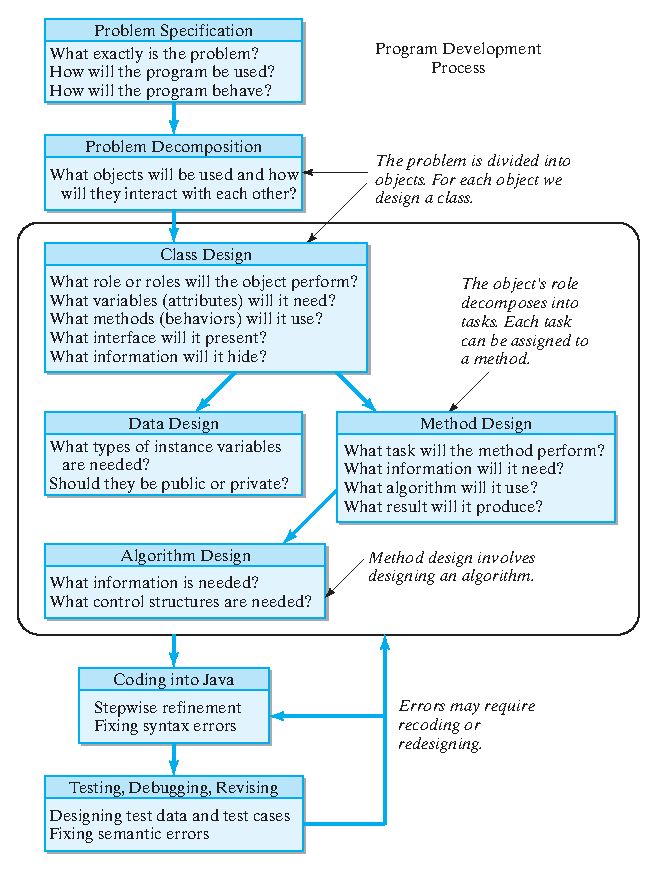
\epsfig{file=ch1-java/figures/progdev.eps}

When should we stop subdividing? How much of a task should be assigned
to a single object or a single method?  The answers to these and
similar questions are not easy.  Good answers require the kind of 
judgment that comes through experience, and frequently there is more
than one good way to design a solution.  Here again, as we learn more
about object-oriented programming, we'll learn more about how to make
these design decisions.

\section{Designing a Riddle Program}

The first step in the program-development process is making sure you
understand the problem (Fig. \ref{fig:progdev}).  Thus, we begin by
developing a detailed specification, which should address three basic
questions:

\begin{BL}
\item  What exactly is the problem to be solved?
\item  How will the program be used?
\item  How should the program behave?
\end{BL}

\noindent In the real world, the problem specification is often
arrived at through an extensive discussion between the customer and
the developer.  In an introductory programming course, the
specification is usually assigned by the instructor.

To help make these ideas a little clearer, let's design an
object-oriented solution to a simple problem.

\BOXDT{{\bf Problem Specification.}
Design a class that will represent a riddle with a given question and
answer.   The definition of this class should make it possible to store
different riddles and to retrieve a riddle's question and answer
independently.
}

\subsection{Problem Decomposition}

\noindent Most problems are too big and too complex to be tackled
all at once. So the next step in the design process is to divide the
\marginnote{Divide and conquer}
problem into parts that make the solution more manageable.  In the
object-oriented approach, a problem is divided into objects, where
each object will handle one specific aspect of the program's overall
job. In effect, each object will become an expert or specialist in
some aspect of the program's overall behavior.

Note that there is some ambiguity here about how far we should go in
decomposing a given program.  This ambiguity is part of the design
process.  How much we should decompose the program before its parts
become ``simple to solve'' depends on the problem we're trying to
solve and on the problem solver.

One useful design guideline for trying to decide what objects
are needed is the following:

\JavaTIP{EFFECTIVE DESIGN}{Looking for Nouns.}{Choosing a program's
objects is often a matter of looking for nouns in the problem
specification.}

\noindent Again, there's some ambiguity involved in this guideline.
For example, the key noun in our current problem is {\it riddle}, so
our solution will involve an object that serves as a model for a
riddle.  The main task of this Java object will be simply to represent
a riddle. Two other nouns in the specification are {\it question} and
{\it answer}. Fortunately, Java has built-in {\tt String} objects that
represent strings of characters such as words or sentences. We can use
two {\tt String} objects for the riddle's question and answer.  Thus,
for this simple problem, we need only design one new type of
object---a riddle---whose primary role will be to represent a riddle's
question and answer.

Don't worry too much if our design decisions seem somewhat mysterious
at this stage. A good understanding of object-oriented design can come
only after much design experience, but this is a good place to start.

\subsection{Object Design}

\noindent Once we have divided a problem into a set of cooperating 
objects, designing a Java program is primarily a matter of designing
and creating the objects themselves. In our example, this means we
must now design the features of our riddle object.  For each object,
we must answer the following basic design questions:

\begin{BL}
\item What role will the object perform in the program?
\vspace{2pt}\item What data or information will it need?
\vspace{2pt}\item What actions will it take?
\vspace{2pt}\item What interface will it present to other objects?
\vspace{2pt}\item What information will it hide from other objects?
\end{BL}

For our riddle object, the answers to these questions are 
shown in Figure~\ref{fig:specs}. Note that although we talk about
``designing an object,'' we are really talking about designing the
object's class. A class defines the collection of objects that belong
to it. The class can be considered the object's {\em type}. This is
the same as for real-world objects. Thus, Seabiscuit is a horse---that
is, Seabiscuit is an object of type horse.  Similarly, an individual
riddle, such as the newspaper riddle, is a riddle.  That is, it is an
object of type Riddle.

The following discussion shows how we arrived at the decisions for the
design specifications for the {\tt Riddle} class, illustrated in
Figure~\ref{fig:specs}.

%%\begin{figure}[tb]
\begin{figure}[h]
\figaproga{100pt}{
\begin{BL}\rm
\item Class Name: Riddle
\item Role: To store and retrieve a question and answer
\item Attributes (Information)
\begin{BSE}
\item question: A variable to store a riddle's question (private)
\item answer: A variable to store a riddle's answer (private)
\end{BSE}
\item Behaviors
\begin{BSE}
\item Riddle(): A method to set a riddle's question and answer
\item getQuestion(): A method to return a riddle's question
\item getAnswer(): A method to return a riddle's answer
\end{BSE}
\end{BL}
}\figaprogb{Design specification for the {\tt Riddle} class.}
%%}\figaprogbleft{Design specification for the {\tt Riddle} class.
{fig:specs}
\end{figure}

The role of the {\tt Riddle} object is to model an ordinary
\marginnote{What is the object's role?}
riddle. Because a riddle is defined in terms of its question and
answer, our {\tt Riddle} object will need some way to store these two
pieces of information. As we learned in Chapter~\ref{chapter-intro}, an instance
variable is a named memory location that belongs to an object. The
fact that the memory location is named, makes it easy to retrieve the
data stored there by invoking the variable's name. For example, to
print a riddle's question we would say something like ``print
question,'' and whatever is stored in {\em question} would be
retrieved and printed.

In general, instance variables are used to store the information that
an object needs to perform its role.
\marginnote{What information will the object need?}
They correspond to what we have been calling the object's
attributes. Deciding on these variables provides the answer to the
question, ``What information does the object need?''  

Next we decide what actions a {\tt Riddle} object will take.
A useful design guideline for actions of objects is the following:

\JavaTIP{EFFECTIVE DESIGN}{Looking for Verbs.}{Choosing the 
behavior of an object is often a matter of looking for verbs in the
problem specification.}

\marginnote{What actions will the object take?}
\noindent For this problem,
the key verbs are {\it set} and {\it retrieve}.  As specified in
Figure~\ref{fig:specs}, each {\tt Riddle} object should provide some
means of setting the values of its question and answer variables and a
means of retrieving each value separately.

Each of the actions we have identified will be encapsulated in a Java
method. As you recall from Chapter~\ref{chapter-intro}, a method is a named section of
code that can be {\em invoked}, or called upon, to perform a
particular action. In the object-oriented approach, calling a method
(method invocation) is the means by which interaction occurs among
objects. Calling a method is like sending a message between
objects. For example, when we want to get a riddle's answer, we
would invoke the {\tt getAnswer()} method.  This is like sending the
message ``Give me your answer.''  One special method, known as a
constructor, is invoked when an object is first created. We will use
the {\tt Riddle()} constructor to give specific values to riddle's
question and answer variables.

In designing an object, we must decide which methods should be made
\marginnote{What interface will it present, and what
information will it hide?}  available to other objects. This
determines what interface the object should present and what
information it should hide from other objects.  In general, those
methods that will be used to communicate with an object are designated
as part of the object's interface. Except for its interface, all other
information maintained by each riddle should be kept ``hidden'' from
other objects. For example, it is not necessary for other objects to
know where a riddle object stores its question and answer. The fact
that they are stored in variables named {\tt question} and {\tt
answer}, rather than variables named {\tt ques} and {\tt ans}, is
irrelevant to other objects.


\JavaTIP{EFFECTIVE DESIGN}{Object Interface.}{An object's interface 
should consist of just those methods needed to communicate with or to
use the object.}

\JavaTIP{EFFECTIVE DESIGN}{Information Hiding.}{An object should 
hide most of the details of its implementation.}


\pagebreak
Taken together, these various design decisions lead to the
\marginfig{chptr01/riddleuml.eps}%
{A UML class diagram representing the  {\tt Riddle} class.}
{fig:ruml}
specification shown in Figure~\ref{fig:ruml}. As our discussion has illustrated,
we arrived at the decisions by asking and answering the right
questions. In most classes the attributes (variables) are
private. This is represented by a minus sign ($-$). In this example,
the operations (methods) are public, which is represented by the plus
sign ($+$). The figure shows that the {\tt Riddle} class has two
hidden (or private) variables for storing data and three visible (or
public) methods that represent the operations that it can perform.

\subsection{Data, Methods, and Algorithms}

\noindent Among the details that must be worked out in
designing a riddle object is deciding what type of data, methods, and
algorithms we need.  There are two basic questions involved:

\begin{BL}
\item  What type of data will be used to represent the information
needed by the riddle?
\item  How will each method carry out its task?
\end{BL}

\noindent Like other programming languages, Java supports a
wide range of different types of data, some simple and some complex.
\marginnote{What type of data will be used?}
Obviously a riddle's question and answer should be represented by
text.  As we noted earlier, Java has a {\tt String} type, which is
designed to store text, which can be considered a string of
characters.

In designing a method, you have to decide what the method will do.  
\marginnote{How will each method carry out its task?}
In order to carry out its task, a method will need certain information,
which it may store in variables.  Plus, it will have to carry out a
sequence of individual actions to perform the task. This is called its
{\bf algorithm}, which is a step-by-step description of the solution
to a problem.  And, finally, you must decide what result the method
will produce.  Thus, as in designing objects, it is important to ask
the right questions:

\begin{BL}
\item  What specific task will the method perform?
\item  What information will it need to perform its task?
\item  What algorithm will the method use?
\item  What result will the method produce?
\end{BL}

\noindent Methods can be thought of as using an algorithm to 
complete a required action.  The algorithm required for the {\tt
Riddle()} constructor is very simple but also typical of constructors
for many classes. It takes two strings and assigns the first to the
{\tt question} instance variable and then assigns the second to the
{\tt answer} instance variable.  The algorithms for the other two
methods for the Riddle class are even simpler.  They are referred to
as {\it get} methods that merely {\it return} or produce the value
that is currently stored in an instance variable.

Not all methods are so simple to design, and not all algorithms are so
\marginnote{Algorithm design}
simple.  Even when programming a simple arithmetic problem, the steps
involved in the algorithm will not always be as obvious as they are
when doing the calculation by hand.  For example, suppose the problem
were to calculate the sum of a list of numbers.  If we were telling our
classmate how to do this problem, we might just say, ``add up all the
numbers and report their total.''  But this description is far too
vague to be used in a program.   By contrast, here's an algorithm that
a program could use:

\begin{NL}
\item  Set the initial value of the sum to 0.
\item  If there are no more numbers to total, go to step 5.
\item  Add the next number to the sum.
\item  Go to step 2.
\item  Report the sum.
\end{NL}

\noindent Note that each step in this algorithm is simple and easy
to follow.   It would be relatively easy to translate it into
Java.  Because English is somewhat imprecise as an algorithmic
language, programmers frequently write algorithms in the programming
\marginnote{Pseudocode}
language itself or in {\bf pseudocode}, a hybrid
language that combines English and programming language structures
without being too fussy about programming language syntax.  For
example, the preceding algorithm might be expressed in pseudocode as
follows:

\begin{jjjlisting}
\begin{lstlisting}
sum = 0
while (more numbers remain)
    add next number to sum
print the sum
\end{lstlisting}
\end{jjjlisting}

Of course, it is unlikely that an experienced programmer would take
the trouble to write out pseudocode for such a simple algorithm.  But
many programming problems are quite complex and require careful design
to minimize the number of errors that the program contains.  In such
situations, pseudocode could be useful.

Another important part of designing an algorithm is to {\it trace}
it---that is, to step through it line by line---on some sample data.
For example, we might test the list-summing algorithm by tracing it on
the list of numbers shown in the margin.
%\begin{table}[h]
%\begin{center}
\marginpar{
\UNTB
\begin{tabular}{rl}
\multicolumn{2}{l}{
\color{cyan}
\rule{8pc}{1pt}}\\[2pt]
%%RAM\UNTBCH{Sum} &\UNTBCH{List of Numbers}
{Sum} & {List of Numbers}
\\[-4pt]\multicolumn{2}{l}{
\color{cyan}
\rule{8pc}{0.5pt}}\\[2pt]
    0        &54 30 20\cr
    54       &30 20\cr
    84       &20\cr
   104       &-
\\[-4pt]\multicolumn{2}{l}{
\color{cyan}
\rule{8pc}{1pt}}
\end{tabular}
\endUNTB
}
%\end{center}
%\end{table}


Initially, the sum starts out at 0 and the
list of numbers contains 54, 30, and 20. On each iteration through the
algorithm, the sum increases by the amount of the next number, and the
list diminishes in size.  The algorithm stops with the correct total
left under the sum column.  While this trace didn't turn up any errors,
it is frequently possible to find flaws in an algorithm by tracing it
in this way.

\subsection{Coding into Java}

\noindent Once a sufficiently detailed design has been developed, it 
is time to start generating Java code.  The wrong way to do this would
be to type the entire program and then compile and run it.  This
generally leads to dozens of errors that can be both demoralizing and
difficult to fix.

The right way to code is to use the principle of {\bf stepwise refinement}. 
\marginnote{Stepwise refinement}
The program is coded in small stages, and after each stage the code is
compiled and tested.  For example, you could write the code for a
single method and test that method before moving on to another part of
the program. In this way, small errors are caught before moving on to
the next stage.

The code for the {\tt Riddle} class is shown in
Figure~\ref{fig:riddleclass}. Even though we have not yet begun
learning the details of the Java language, you can easily pick out the
key parts in this program: the instance variables {\tt question} and
{\tt answer} of type {\tt String}, which are used to store the
riddle's data; the {\tt Riddle()} constructor and the {\tt
getQuestion()} and {\tt getAnswer()} methods make up the interface.
The specific language details needed to understand each of these
elements will be covered in this and the following chapter.

%% proglist ch1/riddle/Riddle.java
\begin{figure}[tb]
\jjjprogstart
\begin{jjjlisting}
\begin{lstlisting}
/*
 * File: Riddle.java
 * Author: Java, Java, Java
 * Description: Defines a simple riddle.
 */
public class Riddle extends Object  // Class header
{                                   // Begin class body
   private String question;       // Instance variables
   private String answer;

   public Riddle(String q, String a) // Constructor method
   {
     question = q;
     answer = a;
   } // Riddle()

   public String getQuestion()   // Instance method
   {
     return question;
   } // getQuestion()

   public String getAnswer()     // Instance method
   {
     return answer;
   } //getAnswer()
} // Riddle class                  // End class body
\end{lstlisting}
\end{jjjlisting}
\jjjprogstop{The {\tt Riddle} class definition.}
{fig:riddleclass}
\end{figure}

\subsection{Syntax and Semantics}
\noindent Writing Java code requires that you know its syntax and 
semantics.  A language's {\bf syntax} is the set of rules
\marginnote{Syntax}
that determines whether a particular statement is correctly
formulated.  As an example of a syntax rule, consider the following
two English statements:


\begin{jjjlisting}
\begin{lstlisting}
The rain in Spain falls mainly on the plain. // Valid
Spain rain the mainly in on the falls plain. // Invalid
\end{lstlisting}
\end{jjjlisting}


\noindent The first sentence follows the rules of English syntax (grammar),
and it means that it rains a lot on the Spanish plain.  The second
sentence does not follow English syntax, and, as a result, it is
rendered meaningless. An example of a Java syntax rule is that a Java
statement must end with a semicolon.

However, unlike in English, where one can still be understood even
when one breaks a syntax rule, in a programming language the syntax
rules are very strict. If you break even the slightest syntax
rule---for example, if you forget just a single semicolon---the
program won't work at all. 


Similarly, the programmer must know the
\marginnote{Semantics}
{\bf semantics} of the language---that is, the meaning of each
statement.  In a programming language, a statement's meaning is
determined by what effect it will have on the program.  For example,
to set the {\tt sum} to 0 in the preceding algorithm, an assignment
statement is used to store the value 0 into the memory location named
{\tt sum}.  Thus, we say that the statement


\begin{jjjlisting}
\begin{lstlisting}
sum = 0;
\end{lstlisting}
\end{jjjlisting}

\noindent assigns 0 to the memory location {\tt sum}, where 
it will be stored until some other part of the program needs it.

Learning Java's syntax and semantics is a major part of learning to
program.  This aspect of learning to program is a lot like learning a
foreign language.  The more quickly you become fluent in the new
language (Java), the better you will be at expressing solutions to
interesting programming problems.  The longer you struggle with Java's
rules and conventions, the more difficult it will be to talk about
problems in a common language.  Also, computers are a lot fussier
about correct language than humans, and even the smallest syntax or
semantic error can cause tremendous frustration.  So, try to be very
precise in learning Java's syntax and semantics.

\subsection{Testing, Debugging, and Revising}

\noindent Coding, testing, and revising a program is an 
repetitive process, one that may require you to repeat the different
program-development stages shown in (Fig.~\ref{fig:progdev}).
According to the stepwise-refinement principle, the process of
developing a program should proceed in small, incremental steps, where
the solution becomes more refined at each step.  However, no matter
how much care you take, things can still go wrong during the coding
process.

A {\it syntax error} is an error that breaks one of Java's syntax
rules. Such errors will be detected by the Java compiler.  Syntax errors 
\marginnote{Syntax errors}
are relatively easy to fix once you understand the error messages
provided by the compiler.  As long as a program contains syntax
errors, the programmer must correct them and recompile the program.
Once all the syntax errors are corrected, the compiler will produce an
executable version of the program, which can then be run.

When a program is run, the computer carries out the steps specified in
the program and produces results.  However, just because a program
runs does not mean that its actions and results are correct.  A
running program can contain {\it semantic errors}, also called 
\marginnote{Semantic errors}
{\it logic errors}.  A semantic error is caused by an error in the
logical design of the program causing it to behave incorrectly,
producing incorrect results.

Unlike syntax errors, semantic errors cannot be detected
automatically.   For example, suppose that a program contains the
following statement for calculating the area of a rectangle:


\begin{jjjlisting}
\begin{lstlisting}
return length + width;
\end{lstlisting}
\end{jjjlisting}

\noindent Because we are adding length and width instead of
multiplying them, the area calculation will be incorrect.  Because
there is nothing syntactically wrong with the expression {\tt length +
width}, the compiler won't detect an error in this statement.  Thus,
the computer will still execute this statement and compute the
incorrect area. 

Semantic errors can only be discovered by testing the program and they
are sometimes very hard to detect. Just because a program appears to
run correctly on one test doesn't guarantee that it contains no
semantic errors. It might just mean that it has not been adequately
tested.

Fixing semantic errors is known as {\it debugging} a program, and when
subtle errors occur it can be the most frustrating part of the whole
program development process.  The various examples presented will
occasionally provide hints and suggestions on how to track down {\it
bugs}, or errors, in your code.  One point to remember when you are
trying to find a very subtle bug is that no matter how convinced you
are that your code is correct and that the bug must be caused by some
kind of error in the computer, the error is almost certainly caused by
your code!

\subsection{Writing Readable Programs}
\noindent Becoming a proficient programmer goes beyond 
simply writing a program that produces correct output.   It also involves 
\marginnote{Programming style}
developing good {\it programming style}, which includes how readable
and understandable your code is.  Our goal is to help you develop a
programming style that satisfies the following principles:

\begin{BL}
\item  {\bf Readability.}
Programs should be easy to read and understand.  Comments should
be used to document and explain the program's code.

\item  {\bf Clarity.}
Programs should employ well-known constructs and standard conventions
and should avoid programming tricks and unnecessarily obscure or
complex code.

\item  {\bf Flexibility.}
Programs should be designed and written so that they are easy to modify.
\end{BL}

\section*{{\color{cyan}Special Topic:} Grace Hopper and \\
\hspace*{20pt}the First Computer Bug}

{\color{cyan}Rear Admiral} Grace Murray Hopper (1906--1992) was a
pioneer computer programmer and one of the original developers of the
COBOL programming language, which stands for {\it CO}mmon {\it
B}usiness-{\it O}riented {\it L}anguage.  Among her many achievements
and distinctions, Admiral Hopper also had a role in coining the term
{\it computer bug}.

In August 1945, she and a group of other programmers were working on
the Mark I, an electro-mechanical computer developed at Harvard that
was one of the ancestors of today's electronic computers.  After
several hours of trying to figure out why the machine was
malfunctioning, someone located and removed a two-inch moth from one
of the computer's circuits.  From then on whenever anything went wrong
with a computer, Admiral Hopper and others would say ``it had bugs in
it.''  The first bug itself is still taped to Admiral Hopper's 1945
log book, which is now in the collection of the Naval Surface Weapons
Center.

In 1991, Admiral Hopper was awarded the National Medal of Technology
by President George Bush.  To commemorate and honor Admiral Hopper's
many contributions, the U.S.~Navy recently named a warship after her.
For more information on Admiral Hopper, see the Web site at

\WWWleft
\begin{jjjlisting}
\begin{lstlisting}[commentstyle=\color{black}\small]
http://www.chips.navy.mil/
\end{lstlisting}
\end{jjjlisting}


\section{Java Language Elements}

\noindent In this section we will introduce some of the key elements 
of the Java language by describing the details of a small program.  We
will look at how a program is organized and what the various parts
do. Our intent is to introduce important language elements, many of
which will be explained in greater detail in later sections.

The program we will study is a Java version of the traditional
HelloWorld program---''traditional'' because practically every
introductory programming text begins with it. When it is run, the
HelloWorld program (Fig.~\ref{fig:helloworld}) just displays the
greeting ``Hello, World!'' on the console.

%% proglist ch1/helloapplication/HelloWorld.java
\begin{figure}[hb]
\jjjprogstart
\begin{jjjlisting}
\begin{lstlisting}[numberstyle=\small,numbers=left]
  /*
   * File: HelloWorld.java
   * Author: Java Java Java
   * Description: Prints Hello, World! greeting.
   */
 public class HelloWorld extends Object // Class header
 {                                   // Start class body
   private String greeting = "Hello, World!";  
   public void greet()               // Method definition
   {                                 // Start method body
       System.out.println(greeting); //  Output statement
   } // greet()                      // End method body
  public static void main(String args[])// Method header
  {                   
    HelloWorld helloworld;         // declare
    helloworld = new HelloWorld(); // create
    helloworld.greet();            // Method call
   }  //  main()
 }  // HelloWorld                  // End class body
\end{lstlisting}
\end{jjjlisting}
\jjjprogstop{The {\tt HelloWorld} application program.}
{fig:helloworld}
\end{figure}


\subsection{Comments}

\noindent The first thing to notice about the {\tt HelloWorld} program 
is the use of comments. A {\bf comment} is a non-executable portion of
a program that is used to document the program. Because comments are
not executable instructions they are just ignored by the compiler.
Their sole purpose is to make the program easier for the programmer to
read and understand.

The {\tt HelloWorld} program contains examples of two types of Java
comments.  Any text contained within /* and */ is considered a
comment.  As you can see in {\tt HelloWorld}, this kind of comment can
extend over several lines and is sometimes called a {\em multiline}
comment.  A second type of comment is any text that follows double
slashes (//) on a line.  This is known as a {\it single-line comment}
because it cannot extend beyond a single line.

When the compiler encounters the beginning marker (/*) of a multiline
comment, it skips over everything until it finds a matching end marker
(*/).  One implication of this is that it is not possible to put one
multiline comment inside of another. That is, one comment cannot be
{\it nested}, or contained, within another comment. The following code
segment illustrates the rules that govern the use of /* and */:


\begin{jjjlisting}
\begin{lstlisting}
/* This first comment begins and ends on the same line. */
/* A second comment starts on this line ...
   and goes on ...
   and this is the last line of the second comment. 
*/ 
/* A third comment starts on this line ...
    /* This is NOT a fourth comment. It is just 
       part of the third comment.
   And this is the last line of the third comment. 
*/
*/  This is an error because it is an unmatched end marker.
\end{lstlisting}
\end{jjjlisting}

\noindent As you can see from this example, it is impossible
to begin a new comment inside an already-started comment because
all text inside the first comment, including /*, is ignored
by the compiler.

\JavaRule{Comments.}{Any text contained within /* and */, which may 
span several lines, is considered a comment and is ignored by the
compiler.  Inserting double slashes (//) into a line turns the rest of
the line into a comment.}

Multiline comments are often used to create a {\em comment block} that
provides useful documentation for the program. In {\tt HelloWorld},
the program begins with a comment block that identifies the name of
file that contains the program and its author and provides a brief
description of what the program does.

For single-line comments, double slashes (//) can be inserted anywhere
\marginnote{Single-line comment}
on a line of code. The result is that the rest of the line is ignored
by the compiler.  We use single-line comments throughout the {\tt
HelloWorld} program to provide a running commentary of its language
elements.

\JavaTIP[false]{PROGRAMMING TIP}{Use of Comments.}%
{A well-written program should begin with a comment block that provides
the name of the program, its author, and a description of what the
program does.}

\subsection{Program Layout}

Another thing to notice about the program is how neatly it is arranged
on the page. This is done deliberately so that the program is easy to
read and understand. In Java, program expressions and statements may
be arranged any way the programmer likes. They may occur one per line,
several per line, or one per several lines.  But the fact that the
rules governing the layout of the program are so lax makes it all the
more important that we adopt a good programming style, one that will
help make programs easy to read.

So look at how things are presented in {\tt HelloWorld}. Notice how
beginning and ending braces, { and }, are aligned, and
note how we use single-line comments to annotate ending braces. Braces
are used to mark the beginning and end of different blocks of code in
a Java program and it can sometimes be difficult to know which
beginning and end braces are matched up. Proper indentation and the
use of single-line comments make it easier to determine how the braces
are matched up.

Similarly, notice how indentation is used to show when one element of
the program is contained within another element. Thus, the elements of
the {\tt HelloWorld} class are indented inside of the braces that mark
the beginning and end of the class. And the statements in the {\tt
main()} method are indented to indicate that they belong to that
method.  Use of indentation in this way, to identify the program's
structure, makes the program easier to read and understand.

\JavaTIP{PROGRAMMING TIP}{Use of Indentation.}
{Indent the code within a block and align the block's opening and closing
braces.  Use a comment to mark the end of a block of code.}

\subsection{Keywords and Identifiers}
\label{subsec:keywords}

\noindent The Java language contains 48 predefined {\it keywords} (Table~\ref{tab:keywords}).
These are words that have special meaning in the language and whose
use is reserved for special purposes. For example, the keywords used
in the HelloWorld program (Fig.~\ref{fig:helloworld}) are: {\tt
class}, {\tt extends}, {\tt private}, {\tt public}, {\tt static}, and
{\tt void}. 

\begin{table}[htb]
%\hphantom{\caption{Java keywords}}
{\caption{Java keywords.\label{tab:keywords}}}
%\begin{tabular}{l}
{\color{cyan}\rule{27pc}{1pt}}\par\vspace{-10pt}
\begin{verbatim}
abstract   default   goto             package       this
boolean    do        if               private       throw
break      double    implements       protected     throws
byte       enum      import           public        transient
case       elses     instanceof       return        try
catch      extend    int              short         void
char       final     interface        static        volatile
class      finally   long             super         while
const      float     native           switch
continue   for       new              synchronized
\end{verbatim}
\par\vspace{-14pt}{\color{cyan}\rule{27pc}{1pt}}
%\end{tabular}
\endTB
\end{table}

Because their use is restricted, keywords cannot be used as the names
of methods, variables, or classes.  However, the programmer can make
up his or her own names for the classes, methods, and variables that
occur in the program, provided that certain rules and conventions are
followed.

The names for classes, methods, and variables are called identifiers,
\marginnote{Identifier syntax}
which follow certain syntax rules:

\JavaRule[false]{Identifier.}{ An {\bf identifier} must begin
with a capital or lowercase letter and may be followed by any number
of letters, digits, underscores (\_), or dollar signs (\$). An
identifier may not be identical to a Java keyword.}

\noindent Names in Java are {\it case sensitive}, which means that
two different identifiers may contain the same letters in the same
order. For example, {\tt thisVar} and {\tt ThisVar} are two different
identifiers.

In addition to the syntax rule that governs identifiers, Java
\marginnote{Identifier style}
programmers follow certain style conventions in making up names for
classes, variables, and methods. By convention, class names in Java
begin with a capital letter and use capital letters to distinguish the
individual words in the name---for example, {\tt HelloWorld} and {\tt
\marginnote{Java naming conventions}
TextField}.  Variable and method names begin with a lowercase letter
but also use capital letters to distinguish the words in the
name---for example, {\tt main()}, {\tt greeting}, {\tt greet()}, {\tt
getQuestion()}, and {\tt getAnswer()}.  The advantage of this convention
is that it is easy to distinguish the different elements in a
program---classes, methods, variables---just by how they are
written. (For more on Java style conventions, see
Appendix A.).

Another important style convention followed by Java programmers
is to choose descriptive identifiers when naming classes,
variables, and methods. This helps to make the program more
readable.

\JavaTIP{PROGRAMMING TIP}{Choice of Identifiers.}%
{To make your program more readable, choose names that describe the
purpose of the class, variable, or method.}

\subsection{Data Types and Variables}
\label{subsec:primitives}


\noindent A computer program wouldn't be very useful if it couldn't
manipulate different kinds of data, such as numbers and strings.  The
operations that one can do on a piece of data depend on the data's
type. For example, you can divide and multiply numbers, but you cannot
do this with strings.  Thus, every piece of data in a Java program is
classified according to its {\bf data type}.

Broadly speaking, there are two categories of data in Java: various
types of objects and eight different types of built-in {\bf primitive
data types}.  In addition to new types of objects that are created by
programmers, Java has many different types of built-in objects. Two
types that we will encounter in this chapter are the {\tt String} and
{\tt PrintStream} objects. Java's primitive types include three
\marginnote{Primitive types}
integer types, three real number types, a character type, and a
boolean type with values true and false.  The names of the primitive
types are keywords like {\tt int} for one integer type, {\tt double}
for one real number type, and {\tt boolean}.

As we noted in Chapter~\ref{chapter-intro}, a variable is a named storage location that
can store a value of a particular type. Practically speaking, you can
think of a variable as a special container into which you can place
values, but only values of a certain type (Fig.~\ref{fig:vars}). For
example, an {\tt int} variable can store values like 5 or -100. A {\tt
String} variable can store values like ``Hello''.  (Actually, this is
not the full story, which is a little more complicated, but we will
get to that in Chapter~\ref{chapter-objects}.)

In the {\tt HelloWorld} class, the instance variable {\tt greeting}
\marginfig{chptr01/vars.eps}{Variables are like {\it typed} containers.}
{fig:vars}
(line 8) stores a value of type {\tt String}. In the {\tt main()}
method, the variable {\tt helloworld} is assigned 
a {\tt HelloWorld} object (line 16).

A {\bf literal value} is an actual value of some type that occurs in a
program. For example, a string enclosed in double quotes, such as
"Hello, World!", is known as a {\tt String} literal. A number such as
45.2 would be an example of a literal of type {\tt double}, and -72
would be an example of a literal of type {\tt int}.  Our HelloWorld
program contains just a single literal value, the "HelloWorld!" {\tt
String}.

\subsection{Statements}
\label{subsec:statements}

A Java program is a collection of statements. A {\bf statement} is a
\marginnote{Executing a program}
segment of code that takes some action in the program. As a program runs,
we say it {\em executes} statements, meaning it carries out the actions
specified by those statements.  In our {\tt HelloWorld} program, statements
of various types occur on lines 8, 11, 15, 16, and 17. Notice that all
of these lines end with a semicolon. The rule in Java is that statements
must end with a semicolon. Forgetting to do so would cause a syntax error.

A {\bf declaration statement} is a statement that declares a variable
of a particular type. In Java, a variable must be declared before it
can be used in a program. Failure to do so would cause a syntax error.
In its simplest form, a declaration statement begins with the
\marginnote{Declaration statement}
variable's type, which is followed by the variable's name, and ends
with a semicolon:

\begin{extract}
{\it Type VariableName} ;
\end{extract}

\noindent A variable's type is either one of the primitive types
we mentioned, such as {\tt int}, {\tt double}, or {\tt boolean}, or
for objects, it is the name of the object's class, such as {\tt
String} or {\tt HelloWorld}. A variable's name may be any legal
identifier, as defined earlier, although the convention in Java is to
begin variable names with a lowercase letter.  In our {\tt HelloWorld}
program, an example a simple declaration statement occurs on line 15:

\begin{jjjlisting}
\begin{lstlisting}
HelloWorld helloworld;                    
\end{lstlisting}
\end{jjjlisting}

\noindent This example declares a variable for an
object.  The variable's name is {\tt helloworld} and its type is {\tt
HelloWorld}, the name of the class that is being defined in our
example.  To take another example the following statements declare two
{\tt int} variables, named {\tt int1} and {\tt int2}:

\begin{jjjlisting}
\begin{lstlisting}
int int1; 
int int2;
\end{lstlisting}
\end{jjjlisting}

\noindent As we noted, an {\tt int} is one of Java's primitive types
and the word {\it int} is a Java keyword. 

Without going into too much detail at this point, declaring a
variable causes the program to set aside enough memory for the type of
data that will be stored in that variable. So in this example, Java
would reserve enough space to store an {\tt int}.

An {\bf assignment statement} is a statement that stores (assigns) a
value in a variable.  An assignment statement uses the equal sign ($=$)
as an assignment operator. In its simplest form, an assignment
statement has a variable on the left hand side of the equals sign and
some type of value on the right hand side. Like other statements, an
assignment statement ends with a semicolon:

\begin{extract}
{\it VariableName} = {\it Value} ;
\end{extract}

\noindent When it executes an assignment statement, Java will first
determine what value is given on the right hand side and then
assign (store) that value to (in) the variable on the left hand
side. Here are some simple examples:
\marginfig{chptr01/assign.eps}{This illustrates how the state of the 
variables {\tt num1} and {\tt num2} changes over the course of
the three assignments, (a), (b), (c), given in the text.}
{fig:assign}

\begin{jjjlisting}
\begin{lstlisting}
greeting = "Hello, World";
num1 = 50;        // (a) Assign 50 to num1
num2 = 10 + 15;   // (b) Assign 25 to num2
num1 = num2;      // (c) Copy num2's value (25) into num1
\end{lstlisting}
\end{jjjlisting}

\noindent In the first case, the value on the right hand 
side is the string literal "Hello, World!", which gets stored in {\tt
greeting}. Of course, {\tt greeting} has to be the right type of
container--in this case, a {\tt String} variable.  In the next case,
the value on the right hand side is 50. So that is the value that gets
stored in {\tt num1}, assuming that {\tt num1} is an {\tt int}
variable. The situation after this assignment is shown in the top
drawing in Figure~\ref{fig:assign}.  In the third case, the value on
the right hand side is 25, which is determined by adding 10 and 15. So
the value that gets assigned to {\tt num2} is 25. After this
assignment we have the situation shown in the middle drawing in the
figure. Of course, this assumes that {\tt num2} is an {\tt int}
variable.  In the last case, the value on the right hand side is 25,
the value that we just stored in the variable {\tt num2}. So, 25 gets
stored in {\tt num1}. This is the bottom drawing in the accompanying
figure.

The last of these examples 

\begin{jjjlisting}
\begin{lstlisting}
num1 = num2;   // Copy num2's value into num1
\end{lstlisting}
\end{jjjlisting}

\noindent can be confusing to beginning programmers, so it is worth
some additional comment. In this case, there are variables on both the
left and right of the assignment operator. But they have very
different meaning. The variable on the right is treated as a value. If
that variable is storing 25, then that is its value. In fact, whatever
occurs on the right hand side of an assignment operator is treated as
a value. The variable on the left hand side is treated as a memory
location. It is where the value 25 will be stored as a result of
executing this statement. The effect of this statement is to copy
the value stored in {\it num2} into {\it num1}, as illustrated
\marginfig{chptr01/assign2.eps}{In the 
assignment {\it num1 = num2;},  {\it num2}'s
value is copied into {\it num1}.}
{fig:assign2}
in Figure~\ref{fig:assign2}.

Java has many other kinds of statements and we will be learning about
these in subsequent examples. The following examples from the {\tt
HelloWorld} program are examples of statements in which a method
is called:

\begin{jjjlisting}
\begin{lstlisting}
System.out.println(greeting);// Call println() method
helloworld.greet();          // Call greet() method
\end{lstlisting}
\end{jjjlisting}

\noindent We will discuss these kinds of statements in greater 
detail as we go along. One final type of statement that should be
mentioned at this point is the {\bf compound statement} (or {\bf
block}), which is a sequence of statements contained within braces
({}).  We see three examples of this in the {\tt
HelloWorld} program. The body of a class definition extends from lines
7 through 19. The body of the {\tt greet()} method is a block that
extends from lines 10 through 12. The body of the {\tt main()} method
is a block that extends from lines 14 to 19.

\subsection{Expressions and Operators}
\label{subsec:expressions}

\noindent The manipulation of data in a program is done by using some
kind of {\em expression} that specifies the action.  An {\bf
expression} is Java code that specifies or produces a value in the
program.  For example, if you want to add two numbers, you would use
an arithmetic expression, such as $num1 + num2$. If you want to
compare two numbers, you would use a relation expression such as $num1
< num2$. As you can see, these and many other expressions in Java
involve the use of special symbols called {\bf operators}. Here we see
the addition operator ($+$) and the less-than operator ($<$). We have
already talked about the assignment operator ($=$).

Java expressions and operators have a type that depends on the type of
data that is being manipulated. For example, when adding two {\tt int}
values, such as $5 + 10$, the expression itself produces an {\tt int}
result.  When comparing two numbers with the less than operator, $num1
< num2$, the expression itself produces a {\tt boolean} type, either
true or false. 

It is important to note that expressions cannot occur on their own.
Rather they occur as part of the program's statements.  Here are some
additional examples of expressions:

\begin{jjjlisting}
\begin{lstlisting}
num = 7      // An assignment expression of type int
num = square(7) // An method call expression of type int
num == 7     // An equality expression of type boolean
\end{lstlisting}
\end{jjjlisting}

\noindent  The first of these is an assignment expression. It has a value 
of {\tt 7}, because it is assigning {\tt 7} to {\tt num}. The second
example is also an assignment expression, but this one has a method
call, {\tt square(7)}, on its right hand side. (We can assume that a
method named {\tt square()} has been appropriately defined in the
program.)  A method call is just another kind of expression. In this
case, it has the value 49.  Note that an assignment expression can be
turned into a stand-alone assignment statement by placing a semicolon
after it.

The third expression is an equality expression, which has the value
{\tt true}, assuming that the variable on its left is storing the
value 7. It is important to note the difference between the assignment
operator ($=$) and the equality operator ($==$).

\JavaRule{Equality and Assignment.} {Be careful not to
confuse {\tt =} and {\tt ==}. The symbol {\tt =} is the assignment
operator. It assigns the value on its right-hand side to the variable
on its left-hand side. The symbol {\tt ==} is the equality
operator. It evaluates whether the expressions on its left- and
right-hand sides have the same value and returns either {\tt true} or
{\tt false}.}

\secEXRHone{Self-Study Exercises}
\begin{SSTUDY}

\item What is stored in the variable {\tt num} after the following
two statements are executed?
\small
\begin{verbatim}
  int num = 11;
  num = 23 - num;
\end{verbatim}
\normalsize

\item Write a statement that will declare a variable of type {\tt int}
called {\tt num2}, and store in it the sum of 711 and 712. 

\end{SSTUDY}


\subsection{Class Definition}

\noindent A Java program consists of one or more class definitions. 
In the {\tt HelloWorld} example, we are defining the {\tt HelloWorld}
class, but there are also three predefined classes involved in the
program. These are the {\tt Object}, {\tt String}, and {\tt System}
classes all of which are defined in the Java class library. Predefined
classes, such as these, can be used in any program.

As the {\tt HelloWorld} program's comments indicate, a class definition
\marginnote{Class header}
has two parts: a {\it class header} and a {\it class body}.  In
general, a class header takes the following form, some parts of which
are optional ({\em opt}):
$$
\hbox{\it ClassModifiers}_{\hbox{\scriptsize\it opt}}\quad
\hbox{\tt class}\quad
\hbox{\it ClassName}\quad
\hbox{\it Pedigree}_{\hbox{\scriptsize\it opt}}
$$

\noindent The class header for the {\tt HelloWorld} class is:

\begin{jjjlisting}
\begin{lstlisting}
public class HelloWorld extends Object
\end{lstlisting}
\end{jjjlisting}

\noindent The purpose of the header is to give the class its name 
({\tt HelloWorld}), identify its accessibility ({\tt public} as
opposed to {\tt private}), and describe where it fits into the Java class
hierarchy (as an extension of the {\tt Object} class). In this case,
the header begins with the optional access modifier, {\tt public},
which declares that this class can be accessed by any other
classes. The next part of the declaration identifies the name of the
class, {\tt HelloWorld}. And the last part declares that {\tt
HelloWorld} is a subclass of the {\tt Object} class. We call this
part of the definition the class's pedigree.

As you recall from Chapter~\ref{chapter-intro}, the {\tt Object} class is the top class
of the entire Java hierarchy. By declaring that {\tt HelloWorld
extends Object}, we are saying that {\tt HelloWorld} is a direct {\em
subclass} of {\tt Object}.  In fact, it is not necessary to declare
explicitly that {\tt HelloWorld} extends {\tt Object} because that is
Java's default assumption. That is, if you omit the extends clause in
the class header, Java will automatically assume that the class is a
subclass of {\tt Object}.

The class's body, which is enclosed within curly brackets ({}),
\marginnote{Class body}
contains the declaration and definition of the elements that make up
the objects of the class.  This is where the object's attributes and
actions are defined. 

\subsection{Declaring an Instance Variable}
\label{subsec:vardecl}

There are generally two kinds of elements declared and defined in the
class body: variables and methods. As we described in Chapter~\ref{chapter-intro}, an
instance variable is a variable that belongs to each object, or
instance, of the class. That is, each instance of a class has its own
copies of the class's instance variables.  The {\tt HelloWorld} class
has a single instance variable, ({\tt greeting}), which is declared as
follows:

\begin{jjjlisting}
\begin{lstlisting}
private String greeting = "Hello, World!"; 
\end{lstlisting}
\end{jjjlisting}

\noindent In general, an instance variable declaration has the following
syntax, some parts of which are optional:

$$
\hbox{\it Modifiers}_{\hbox{\scriptsize\it opt}}\quad
\hbox{\it Type}\quad
\hbox{\it VariableName}\quad
\hbox{\it InitializerExpression}_{\hbox{\scriptsize\it opt}}
$$

\noindent Thus, a variable declaration begins with optional modifiers. 
In declaring the {\tt greeting} variable, we use the access modifier,
{\tt private}, to declare that {\tt greeting}, which belongs to the
{\tt HelloWorld} class, cannot be directly accessed by other
objects. The next part of the declaration is the variable's type. In
\marginnote{Information hiding}
this case, the {\tt greeting} variable is a {\tt String}, which means
that it can store a string object.  The type is followed by the name
of the variable, in this case ({\tt greeting}). This is the name that
is used to refer to this memory location throughout the class. For
example, notice that the variable is referred to on line 11 where it
is used in a {\tt println()} statement.

The last part of the declaration is an optional initializer
expression. In this example, we use it to assign an initial value,
``Hello, World!,'' to the {\tt greeting} variable.  

\subsection{Defining an Instance Method}

Recall that a method is a named section of code that can be called or
invoked to carry out an action or operation.  In a Java class, the
methods correspond to the object's behaviors or actions. The {\tt
HelloWorld} program has two method definitions: the {\tt greet()}
method and the {\tt main()} method.

A method definition consists of two parts: the method header and the
method body. In general, a method header takes the following
form, including some parts which are optional:

$$
\hbox{\it Modifiers}_{\hbox{\scriptsize\it opt}}\quad
\hbox{\it ReturnType}\quad
\hbox{\it MethodName}\quad
\hbox{\tt (}\quad
\hbox{\it ParameterList}_{\hbox{\scriptsize\it opt}}
\hbox{\tt )}\quad
$$

\noindent As with a variable declaration, a method definition
begins with optional modifiers. For example, the definition of the
{\tt greet()} method on line 9 uses the access modifier, {\tt public},
to declare that this method can be accessed or referred to by other
classes.  The {\tt main()} method, whose definition begins on line 13,
is a special method, and is explained in the next section.

The next part of the method header is the method's return type. This
is the type of value, if any, that the method returns.  Both of the
methods in {\tt HelloWorld} have a return type of {\tt void}. This
means that they don't return any kind of value. Void methods just
execute the sequence of statements given in their bodies.  For an
example of a method that does return a value, take a look again at the
declaration of the {\tt getQuestion()} method in the {\tt Riddle}
class, which returns a {\tt String} (Fig.~\ref{fig:riddleclass}).

The method's name follows the method's return type. This is the name
that is used when the method is called. For example, the {\tt greet()}
method is called on line 17.

Following the method's name is the method's parameter list. A {\bf
parameter} is a variable that temporarily stores data values that are
being passed to the method when the method is called. Some methods,
such as the {\tt greet()} method, do not have parameters, because they
are not passed any information. For an example of a method that does
have parameters, see the {\tt Riddle()} constructor, which contains
parameters for the riddle's question and answer
(Fig.~\ref{fig:riddleclass}).  

The last part of method definition is its body, which contains a
sequence of executable statements. An {\bf executable statement} is a
Java statement that takes some kind of action when the program is run.
For example, the statement in the {\tt greet()} method,

\begin{jjjlisting}
\begin{lstlisting}
System.out.println(greeting);   //  Output statement
\end{lstlisting}
\end{jjjlisting}

\noindent prints a greeting on the console. 

\subsection{Java Application Programs}

The HelloWorld program is an example of a Java {\bf application
program}, or a Java application, for short.  An application program is
a stand-alone program, ``stand-alone'' in the sense that it does not
depend on any other program, like a Web browser, for its execution.
Every Java application program must contain a {\tt main()} method,
which is where the program begins execution when it is run. For a
program that contains several classes, it is up to the programmer to
decide which class should contain the {\tt main()} method. We don't
have to worry about that decision for the HelloWorld, because it
contains just a single class.

Because of its unique role as the starting point for every
Java application program,  it is very important that the header for
the main method be declared exactly as shown in the {\tt HelloWorld}
class:

\begin{jjjlisting}
\begin{lstlisting}
public static void main(String args[])   
\end{lstlisting}
\end{jjjlisting}

\noindent It must be declared {\tt public} so it can be accessed
from outside the class that contains it.  The {\tt static} modifier
\marginnote{Class method}
is used to designate {\tt main()} as a class method. As you might
recall from Chapter 0, a class method is a method that is associated
directly with the class that contains it rather than with the objects
of the class. A class method is not part of the class's
objects. Unlike instance methods, which are invoked through a class's
objects, a class method is called through the class itself. Thus, a
class method can be called even before the program has created objects
of that class. Because of {\tt main()}'s special role as the program's
starting point, it is necessary for {\tt main()} to be a class method
because it is called, by the Java runtime system, before the program
has created any objects.

The {\tt main()} method has a {\tt void} return type, which means it
does not return any kind of value. Finally, notice that {\tt main()}'s
parameter list contains a declaration of some kind of {\tt String}
parameter named {\it args}. This is actually an array that can be used
to pass string arguments to the program when it is started up. We
won't worry about this feature until our chapter on arrays.

\subsection{Creating and Using Objects}

\noindent The body of the {\tt main()} method is where the 
{\tt HelloWorld} program creates its one and only object.  Recall that
when it is run the {\tt HelloWorld} program just prints the ``Hello
World!'' greeting. As we noted earlier, this action happens in the
{\tt greet()} method. So in order to make this action happen, we need
to call the {\tt greet()} method. However, because the {\tt greet()}
method is an instance method that belongs to a {\tt HelloWorld}
object, we first need to create a {\tt HelloWorld} instance. This is
what happens in the body of the {\tt main()} method
(Fig.~\ref{fig:helloworld}).

The {\tt main()} method contains three statements:

\begin{jjjlisting}
\begin{lstlisting}
HelloWorld helloworld;          // Variable declaration
helloworld = new HelloWorld();  // Object instantiation
helloworld.greet();             // Method invocation
\end{lstlisting}
\end{jjjlisting}

\noindent The first statement declares a variable of type 
{\tt HelloWorld}, which is then assigned a {\tt HelloWorld} object. 
The second statement creates a {\tt HelloWorld}
object. This is done by invoking the {\tt HelloWorld()} constructor
method. Creating an object is called {\bf object instantiation}
because you are creating an instance of the object.  Once a {\tt
HelloWorld} instance is created, we can use one of its instance
methods to perform some task or operation. Thus, in the third
statement, we call the {\tt greet()} method, which will print ``Hello
World!'' on the console.

If you look back at the {\tt HelloWorld} program in
Figure~\ref{fig:helloworld} you won't find a definition of a
\marginnote{Default constructor}
constructor method.  This is not an error because Java will provide a
default constructor if a class does not contain a constructor
definition. The {\bf default constructor} is a trivial constructor
method, ``trivial'' because its body contains no statements. Here
is what the default {\tt HelloWorld()} constructor would look like:

\begin{jjjlisting}
\begin{lstlisting}
public HelloWorld() {  }  // Default constructor
\end{lstlisting}
\end{jjjlisting}

\noindent For most of the classes we design, we will design our
own constructors, just as we did in the {\tt Riddle} class
(Fig.~\ref{fig:riddleclass}).  We will use constructors to assign
initial values to an object's instance variables or to perform other
kinds of tasks that are needed when an object is created. Because the
{\tt HelloWorld} object doesn't require any startup tasks, we can make
do with the default constructor.

The {\tt HelloWorld} program illustrates the idea that an
\marginnote{Interacting objects}
object-oriented program is a collection of interacting objects.
Although we create just a single {\tt HelloWorld} object in the {\tt
main()} method, there are two other objects used in the program. One
is the {\tt greeting}, which is a {\tt String} object consisting of
the string ``Hello, World!''.  The other is the {\tt System.out}
object, which is a special Java system object used for printing.
	
\subsection{Java JFrames}

Java cann run a program in a {\bf JFrame} so that the output 
and interaction occurs in a Window (or Frame). Figure~\ref{fig:hellojframe} shows a Java program named {\tt
HelloWorldSwing}. This program does more or less the same thing as
%% proglist ch1/hellojframe/HelloWorldSwing.java
\begin{figure}[h!]
\jjjprogstart
\begin{jjjlisting}
\begin{lstlisting}
 /** File: HelloWorldSwing program */

import javax.swing.JFrame; // Import class names
import java.awt.Graphics;
import java.awt.Canvas;

public class HelloWorldCanvas extends Canvas // Class header
{                                            
    // Start of body
    public void paint(Graphics g)           
        // The paint method
    {
        g.drawString("Hello, World!", 10, 10);
    }  // End of paint

    public static void main(String[] args){
        HelloWorldCanvas c = new HelloWorldCanvas();
        JFrame f = new JFrame();
        f.add(c);
        f.setSize(150,50);
        f.setVisible(true);
    }
}  // End of HelloWorldCanvas

\end{lstlisting}
\end{jjjlisting}
\jjjprogstop{{\tt Hello\-World\-Canvas} program.}
{fig:hellojframe}
\end{figure}
the {\tt HelloWorld} application---it displays the ``Hello, World!'' 
greeting. The difference is that it displays the greeting within
a Window rather than directly on the console. 

As in the case of the {\tt HelloWorld} console application program, {\tt
Hello\-World\-Canvas} consists of a class definition.  It contains a
single method definition, the {\tt paint()} method, which
contains a single executable statement:

\begin{jjjlisting}
\begin{lstlisting}
g.drawString("Hello, World!",10,10);
\end{lstlisting}
\end{jjjlisting}

\noindent This statement displays the ``Hello, World!'' message
directly in a Window. 
The {\tt drawString()} method is one of the many
drawing and painting methods defined in the {\tt Graphics} class.
Every Java Canvas comes with its own {\tt Graphics} object, which is
referred to here simply as {\tt g}. Thus, we are using that object's
{\tt drawString()} method to draw on the window. Don't worry
if this seems a bit mysterious now. We'll explain it more fully when
we take up graphics examples again.


The {\tt HelloWorldSwing} also contains some elements, such as the
{\tt import} statements, that we did not find in the {\tt HelloWorld}
application. We will now discuss those features.


\subsection{Java Library Packages} 

Recall that the {\tt HelloWorld} application program used two
pre-defined classes, the {\tt String} and the {\tt System}
classes. Both of these classes are basic language classes in Java.
The {\tt HelloWorldSwing} program also uses pre-defined classes, such
as {\tt JFrame} and {\tt Graphics}. However, these two classes are not
part of Java's basic language classes.  To understand the difference
between these classes, it will be necessary to talk briefly about
how the Java class library is organized.

A {\bf package} is a collection a inter-related classes in the Java
class library. For example, the {\tt java.lang} package contains
classes, such as {\tt Object}, {\tt String}, and {\tt System}, that
are central to the Java language. Just about all Java programs use
classes in this package. The {\tt java.awt} package provides classes,
such as {\tt Button}, {\tt TextField}, and {\tt Graphics}, that are
used in graphical user interfaces (GUIs).  The {\tt java.net} package
provides classes used for networking tasks, and the {\tt java.io}
package provides classes used for input and output operations.

All Java classes belong to some package, including those that are
programmer defined. To assign a class to a package, you would provide
a {\tt package} statement as the first statement in the file that
contains the class definition. For example, the files containing the
definitions of the classes in the {\tt java.lang} package all begin
with the following statement.

\begin{jjjlisting}
\begin{lstlisting}
package java.lang;
\end{lstlisting}
\end{jjjlisting}

\noindent If you omit {\tt package} statement, as we do for the
programs in this book, Java places such classes into an unnamed
default package. 

Thus, for any Java class, its full name includes the name of the
package that contains it. For example, the full name for the {\tt
System} class is {\tt java.lang.System} and the full name for the {\tt
String} class is {\tt java.lang.String}.  Similarly, the full name for
the {\tt Graphics} class is {\tt java.awt.Graphics}.  In short, the
full name for a Java class takes the following form:

$$
\hbox{\it package.class}\quad
$$

\noindent In other words, the full name of any class provides
its package name as a prefix.

Of all the packages in the Java library, the {\tt java.lang} package
is the only one whose classes are available by their shorthand names
to all Java programs. This means that when a program uses a class from
the {\tt java.lang} package, it can refer to it simply by its class
name. For example, in the {\tt HelloWorld} program we referred
directly to the {\tt String} class rather than to {\tt
java.lang.String}.

\subsection{The {\tt import} Statement}

The {\tt import} statement makes Java classes available to programs
under their abbreviated names. Any public class in the Java class
library is available to a program by its fully qualified name.  Thus,
if a program was using the {\tt Graphics} class, it could always refer
to it as {\tt java.awt.Graphics}.  However, being able to refer to
{\tt Graphics} by its shorthand name, makes the program a bit
shorter and more readable.

The {\tt import} statement doesn't actually load classes into the
program. It just makes their abbreviated names available.  For
example, the import statements in {\tt HelloWorldSwing} allow us to
refer to the {\tt JFrame}, {\tt Canvas}, and {\tt Graphics} classes by their
abbreviated names (Fig.~\ref{fig:hellojframe}).

The {\tt import} statement takes two possible forms:
$$
\hbox{\tt import }\quad
\hbox{\it package.class}\quad
$$
$$
\hbox{\tt import }\quad
\hbox{\it package.*}\quad\\
$$

\noindent The first form allows a specific class to be known
by its abbreviated name. The second form, which uses the asterisk as a
wildcard characters ('*'), allows all the classes in the specified
package to be known by their short names. The {\tt import} statements
in {\tt HelloWorldSwing} are examples of the first form. The
following example,

\begin{jjjlisting}
\begin{lstlisting}
import java.lang.*;
\end{lstlisting}
\end{jjjlisting}

\noindent allows all classes in the {\tt java.lang} package to
be referred to by their class names alone. In fact, this particular
{\tt import} statement is implicit in every Java program.

\subsection{Qualified Names in Java}
\label{subsec:qualifiednames}

\noindent In the previous subsections we have seen several
examples of names in Java programs that used {\it dot notation}.  A
{\bf qualified name} is a name that is separated into parts using
Java's dot notation. Examples include package names, such as {\tt
java.awt}, class names, such as {\tt javax.swing.JFrame}, and
even method names, such as {\tt helloworld.greet()}.

Just as in our natural language, the meaning of a name within a Java
program depends on the context.  For example, the expression {\tt
helloworld.greet()} refers to the {\tt greet()} method, which
belongs to the {\tt HelloWorld} class.  If we were using this
expression from within that class, you wouldn't need to qualify
the name in this way.  You could just refer to {\tt greet()} and it
would be clear from the context which method you meant.

This is no different than using someone's first name (``Kim'') when
there's only one Kim around, but using a full name (``Kim Smith'')
when the first name alone would be too vague or ambiguous.

One thing that complicates the use of qualified names is that they are
used to refer to different kinds of things within a Java program.  But
this is no different, really, than in our natural language, where
names (``George Washington'') can refer to people, bridges,
universities, and so on. Here again, just as in our natural language,
Java uses the context to understand the meaning of the name.  For
example, the expression {\tt java.lang.System} refers to the {\tt
System} class in the {\tt java.lang} package, whereas the expression
{\tt System.out.print()} refers to a method in the {\tt System.out}
object.

How can you tell these apart?  Java can tell them apart because the
first one occurs as part of an {\tt import} statement, so it must be
referring to something that belongs to a package.  The second expression
would only be valid in a context where a method invocation is allowed.
You will have to learn a bit more about the Java language before
you'll be able to completely understand these names, but the following
provide some naming rules to get you started.

\JavaRule{Library Class Names.}{By convention, class
names in Java begin with an uppercase letter.  When referenced as part
of a package, the class name is the last part of the name.  For
example, {\tt java.lang.System} refers to the {\tt System} class in
the {\tt java.lang} package.}

\JavaRule{Dot Notation.}{Names expressed in Java's
{\it dot notation} depend for their meaning on the context in which
they are used.  In qualified names---that is, names of the form
X.Y.Z---the last item in the name (Z) is the {\it referent}---that is,
the element being referred to.  The items that precede it (X.Y.) are
used to qualify or clarify the referent.}

\noindent The fact that names are context dependent in this way certainly
complicates the task of learning what's what in a Java program.   Part
of learning to use Java's built-in classes is learning where a
particular object or method is defined.  It is a syntax error if the
Java compiler can't find the object or method that you are
referencing.

\JavaTIP{DEBUGGING TIP}{Not Found Error.}{If Java cannot find the item you
are referring to, it will report an ``X not found'' error, where X is
the class, method, variable, or package being referred to.}

\section{Editing, Compiling, and 
Running a Java Program}

\noindent In this section we discuss the nuts and bolts of 
how to compile and run a Java program. Because we are exploring two 
different varieties of Java programs, console applications and Swing
applications, 
the process differs slightly for each variety.  We have already discussed some of the main
language features of console and Swing applications, so in this section
we focus more on features of the programming environment itself.
Because we do not assume any particular programming environment in
this book, our discussion will be somewhat generic.  However,
we do begin with a brief overview of the types of programming
environments one might encounter.

\subsection{Java Development Environments}

\noindent A Java programming environment typically consists of several 
programs that perform different tasks required to edit, compile, and
run a Java program.  The following description will be based on the
software development environment provided by Oracle, the
company that owns and maintains Java. It is currently known as the {\it Java
Platform, Standard Edition 8.0 (Java SE 8)}. Versions of Java SE are
available for various platforms, including Linux, Windows, and
macOS computers.  Free downloads are available at Sun's Web site
at {\tt http://www.oracle.com/technetwork/java/}. (For more details
about the Java SE,
see Appendix~\ref{appendix-jdk}.)

In some cases, the individual programs that make up the Java SE are
available in a single program development environment, known as an
{\it integrated development environment (IDE)}. Some examples include
Eclipse, jGrasp, and Oracle's own NetBeans
IDE.  Each of these provides a complete development package for
editing, compiling, and running Java applications on
a variety of platforms, including Linux, macOS, and Windows.

Figure~\ref{fig:compile} illustrates the process involved in creating
and running a Java program.  The discussion that follows here assumes
\begin{figure}[tb]
\figaleft{chptr01/compile.eps}{Editing, compiling, and running
%%%\figa{chptr01/compile.eps}{Editing, compiling, and running
{\tt HelloWorld.java}.
} {fig:compile}

\end{figure}
that you are using the Java SE as your development environment to edit,
compile and run the example program.  If you are using some other
environment, you will need to read the documentation provided with the
software to determine exactly how to edit, compile, and run Java
programs in that environment.


%\begin{SLlist}
%\item  {\bf Step 1. Editing a Program}
\subsection{Editing a Program}

\noindent Any text editor may be used to edit the program by
merely typing the program and making corrections as needed.  Popular
Unix and Linux editors include {\tt vim} and {\tt emacs}. These
editors are also available on macOS and Windows. However, free macOS
editors include {\tt TextMate} and {\tt TextWrangler}, and Windows has
{\tt Notepad++} for free.  

As we have seen, a Java program consists of one or more class
definitions.  We will follow the convention of placing each class
definition in its own file. (The rule in Java is that a source file
may contain only one {\tt public} class definition.)  The files
containing these classes' definitions must be named {\it
ClassName.java} where {\it ClassName} is the name of the {\tt public}
Java class contained in the file.

\JavaRule[false]{File Names.}{A file that defines a {\tt public}
Java class named {\tt ClassName} must be saved in a text
file named {\tt ClassName.java}. Otherwise an error will result.}

\noindent For example, in the case of our {\tt HelloWorld} application program, 
the file must be named {\tt HelloWorld.java}, and for {\tt
HelloWorldSwing}, it must be named {\tt HelloWorldSwing.java}.
Because Java is {\em case sensitive}, which means that Java pays
attention to whether a letter is typed uppercase or lowercase, it
would be an error if the file containing the {\tt HelloWorld} class
were named {\tt helloworld.java} or {\tt Helloworld.java}.  The error
in this case would be a semantic error. Java would not be able to find
the {\tt HelloWorld} class because it will be looking for a file named
{\tt HelloWorld.java}.

\JavaRule{Case Sensitivity.} {Java is case sensitive,
which means that it treats {\tt helloWorld} and {\tt Helloworld}
as different names.}

\subsection{Compiling a Program}

\noindent Recall that before you can run a Java source program you
have to compile it into the Java  bytecode, the intermediate code
understood by the Java Virtual Machine (JVM).  Source code for both
applets and applications must be compiled.  To run a Java
program, whether an applet or an application, the JVM is then used to
interpret and execute the bytecode.

The Java SE comes in two parts, a runtime program, called the {\it Java
Runtime Environment (JRE)} and a development package, called the {\em
Software Development Kit (SDK)}. If you are just going to run Java
programs, you need only install the JRE on your computer. In order to
run Java applets, browsers, such as Internet Explorer and Netscape
Navigator, must contain a plugin version of the JRE.  On the other
hand, if you are going to be developing Java programs, you will need
to install the SDK as well.

The Java SDK compiler is named {\tt javac}. In some
environments---such as within Linux or at the Windows command prompt
---{\tt HelloWorld.java} would be compiled by typing the
following command at the system prompt:

\begin{jjjlisting}
\begin{lstlisting}
javac HelloWorld.java
\end{lstlisting}
\end{jjjlisting}

\noindent As Figure~\ref{fig:compile} illustrates, if the 
{\tt HelloWorld.java} program does not contain errors, the result of
this command is the creation of a Java bytecode file named {\tt
HelloWorld.class}---a file that has the same prefix as the source file
but with the suffix {\tt .class} rather than {\tt .java}.  By default,
the bytecode file will be placed in the same directory as the source
file. If {\tt javac} detects errors in the Java code, a list of error
messages will be printed.

\subsection{Running a Java Application Program}

\noindent In order to run (or execute) a program on any computer, 
the program's {\it executable code} must be loaded into the
computer's main memory.  For Java environments, this means that the
program's {\tt .class} file must be loaded into the computer's memory,
where it is then interpreted by the Java Virtual Machine.  To run a
Java program on Linux systems or at the Windows command prompt, type

\begin{jjjlisting}
\begin{lstlisting}
java HelloWorld
\end{lstlisting}
\end{jjjlisting}

\noindent on the command line.  This command loads the JVM,
which will then load and interpret the application's bytecode
({\tt HelloWorld.class}). The ``HelloWorld'' string will be displayed on
the command line.

On Macintosh systems, or within an IDE, which do not typically 
have a command line interface, you would select the compile and run
commands from a menu.  Once the code is compiled, the run command will
cause the JVM to be loaded and the bytecode to be interpreted.  The
``Hello, World!''  output would appear in a text-based window that
automatically pops up on your computer screen.  In any case,
regardless of the system you use, running the {\tt HelloWorld}
console application program will cause the ``Hello, World!'' message to be
displayed on some kind of standard output device (Fig.~\ref{fig:stdout}).
\marginfigscaled{chptr01/1f4.png}{0.5}{Compiling and Running the {\tt HelloWorld.java} console application
program.}
{fig:stdout}


\subsection{Running a Java Swing Program}
\label{subsec:swing}

When you run a  Java Swing Program, there is typically no console
output. You only see your output in the Window (JFrame) that your
Graphics are displayed in. This makes automated testing more difficult
since you need to visually inspect that the program is working correctly.

When you run

\begin{jjjlisting}
\begin{lstlisting}
java HelloWorldSwing
\end{lstlisting}
\end{jjjlisting}

\noindent A window will open, and you won't be able to type in the
console until you close the window, quit the program, or type ctl-c to
send a kill signal to the Swing program. The
result of running, as shown in Figure~\ref{fig:hello}, is that the ``Hello, World!'' message
will be displayed within it's own window.

\vspace*{2pc}
\section{From the Java Library: System and \\PrintStream}
\label{sec:systemclass}
\WWWjava 
Java comes with a library of classes that can be used to perform
common tasks. The Java class library is organized into a set
of packages, where each package contains a collection of related
classes.  Throughout the book we will identify library classes and
explain how to use them. In this section we introduce the {\tt System}
and {\tt PrintStream} classes, which are used for printing a program's
output.

Java programs need to be able to accept input and to display output.
Deciding how a program will handle input and output (I/O) is part of
designing its {\em user interface}, a topic we take up in detail in
Chapter 4. The simplest type of user interface is a {\it command-line
interface}, in which input is taken from the command line through the
keyboard, and output is displayed on the console.  Some Java
applications use this type of interface. Another type of user
interface is a {\it Graphical User Interface (GUI)}, which uses
buttons, text fields, and other graphical components for input and
output. Java applets use GUIs as do many Java applications.  Because
we want to be able to write programs that generate output, this
\marginfig{chptr01/1f6.png}{Running
{\tt HelloWorldSwing.java} graphical program.}
{fig:hello}

section describes how Java handles simple console output.

In Java, any source or destination for I/O is considered a {\it
stream} of bytes or characters. To perform output, we insert bytes or
characters into the stream. To perform input, we extract bytes or
characters from the stream.  Even characters entered at a keyboard, if
considered as a sequence of keystrokes, can be represented as a
stream.


There are no I/O statements in the Java language.  Instead, I/O is
handled through methods that belong to classes contained in the {\tt
java.io} package\index{java.io package}. We have already seen how the
output method {\tt println()} is used to output a string
to the console. For example, the following {\tt println()} statement

\begin{jjjlisting}
\begin{lstlisting}
System.out.println("Hello, World");
\end{lstlisting}
\end{jjjlisting}

\noindent prints the message ``Hello, World'' on the
Java console.  Let's now examine this statement more carefully to see
how it makes use of the Java I/O classes.

The {\tt java.io.PrintStream} class is Java's printing expert, so to
speak. It contains a variety of {\tt print()} and {\tt println()}
methods that can be used to print all of the various types of data we
find in a Java program.  A partial definition of {\tt PrintStream} is
shown in Figure~\ref{fig:printstreamUML}. Note
%\begin{figure}[tb]
%\begin{graphic}
%%\marginfig{CHPTR01:printstreamUML.eps}
\marginfig{chptr01/printstr.eps}
%\begin{fig}
{A UML class diagram of the {\tt PrintStream} class.}
{fig:printstreamUML}
%\figa
%\end{fig}
%}
%\end{graphic}
%\end{figure}
that in this case the {\tt PrintStream} class has no attributes,
just operations or methods.

Because the various {\tt print()} and {\tt println()} methods are
instance methods of a {\tt PrintStream} object, we can only use them
by finding a {\tt PrintStream} object and ``telling'' it to print data
for us.  As shown in Figure~1.15, Java's {\tt java.lang.System} class
contains three predefined streams, including two {\tt PrintStream}
objects. This class has public ($+$) attributes.  None of its public
methods are shown here. 

Both the {\tt System.out} and {\tt System.err} objects can be used to
write output to the console.  As its name suggests, the {\tt err}
stream is used primarily for error messages, whereas the {\tt out}
stream is used for other printed output.  Similarly, as its name
suggests, the {\tt System.in} object can be used to handle input,
which will be covered in Chapter~2.

The only difference between the {\tt print()} and {\tt println()}
methods is that {\tt println()} will also print a carriage return and
line feed after printing its data, thereby allowing subsequent output
to be printed on a new line.  For example, the following statements

\begin{jjjlisting}
\begin{lstlisting}
System.out.print("hello");         
System.out.println("hello again"); 
System.out.println("goodbye"); 
\end{lstlisting}
\end{jjjlisting}

\noindent would produce the following output:

\begin{jjjlisting}
\begin{lstlisting}
hellohello again
goodbye
\end{lstlisting}
\end{jjjlisting}

%\begin{figure}
%\begin{graphic}
%%\marginfig{CHPTR01:systemUML.eps}%
\marginfig{chptr01/systemum.eps}%
%\begin{fig}
{The {\tt System} class.}
{fig:systemUML}

%\figa
%\end{fig}
%}
%\end{graphic}
%\end{figure}

\noindent Now that we know how to use Java's printing expert,
let's use it to ``sing'' a version of ``Old MacDonald Had a
Farm.'' As you might guess, this program will simply consist of a
sequence of {\tt System.out.println()} statements each of which prints a
line of the verse.  The complete Java application program is shown in
Figure~\ref{fig:oldmac}.

\begin{figure}[h]
\jjjprogstart
\begin{jjjlisting}
\begin{lstlisting}
public class OldMacDonald
{
   public static void main(String args[])   // Main method
   {
     System.out.println("Old MacDonald had a farm");
     System.out.println("E I E I O.");
     System.out.println("And on his farm he had a duck.");
     System.out.println("E I E I O.");
     System.out.println("With a quack quack here.");
     System.out.println("And a quack quack there.");
     System.out.println("Here a quack, there a quack,");
     System.out.println("Everywhere a quack quack.");
     System.out.println("Old MacDonald had a farm");
     System.out.println("E I E I O.");
   }  // End of main
}  // End of OldMacDonald
\end{lstlisting}
\end{jjjlisting}
\jjjprogstop{The {\tt Old\-Mac\-Donald.java} class.}
{fig:oldmac}

\end{figure}

This example illustrates the importance of using the Java class
library.  If there's a particular task we want to perform, one of the
first things we should ask is whether there is already an ``expert''
in Java's class library that performs that task.  If so, we can use
methods provided by the expert to perform that particular task.

\JavaTIP[false]{EFFECTIVE DESIGN}{Using the Java Library.} {Learning how to use
classes and objects from the Java class library is an important
part of object-oriented programming in Java.}

\secEXRHone{Self-Study Exercises}
\begin{SSTUDY}
\marginnote{\small\tt
**********\\
\mbox{*}\mbox{ }**\mbox{ }\mbox{ }**\mbox{ }*\\
\mbox{*}\mbox{ }\mbox{ }\mbox{ }**\mbox{ }\mbox{ }\mbox{ }*\\
\mbox{*}\mbox{ }*\mbox{ }\mbox{ }\mbox{ }\mbox{ }*\mbox{ }*\\
\mbox{*}\mbox{ }\mbox{ }****\mbox{ }\mbox{ }*\\
\mbox{*}*********
}

\item One good way to learn how to write programs is to modify existing
programs.   Modify the {\tt OldMacDonald} class to ``sing'' one more
verse of the song.

\item Write a Java class that prints the design shown on the left.

\end{SSTUDY}

\secSMH{Chapter Summary}
\secKTH{Technical Terms}
\begin{KT}
algorithm

applet

application program

assignment statement

comment 

compound statement (block)

data type

declaration statement

default constructor

executable statement

expression

identifier

literal value

object instantiation

operator

package

parameter

primitive data type

pseudocode

qualified name

semantics

statement

stepwise refinement

syntax

\end{KT}


\secSMHtwo{Summary of Important Points}
\begin{BL}

\item  Good program design requires that each object and method
have a well-defined role and clear definition of what information is needed
for the task and what results will be produced.

\item Good program design is important; the sooner you start coding, 
the longer the program will take to finish. Good program design
strives for readability, clarity, and flexibility.

\item  Testing a program is very important and must be done with
care, but it can only reveal the presence of bugs, not their absence.

\item  An algorithm is a step-by-step process that solves some
problem.  Algorithms are often described in pseudocode, a hybrid
language that combines English and programming language constructs.

\item  A syntax error occurs when a statement breaks a Java 
syntax rules.  Syntax errors are detected by the compiler.  A semantic
error is an error in the program's design and cannot be detected by
the compiler.

\item  Writing Java code should follow the stepwise refinement process.

\item Double slashes (//) are used to make a single-line comment.
Comments that extend over several lines must begin with /* and end
with */. 

\item  An {\it identifier} must begin with a letter of the
alphabet and may consist of any number of letters, digits, and the
special characters \_ and \$. An identifier cannot be identical to a
Java keyword. Identifiers are case sensitive.

\item  A {\it keyword} is a term that has special meaning in the
Java language (Table~1.1).

\item  Examples of Java's  {\it primitive data types} include
the {\tt int}, {\tt boolean}, and {\tt double} types. 

\item A variable is a named storage location. In Java, a 
variable must be declared before it can be used.

\item A literal value is an actual value of some type, such as
a {\tt String} ("Hello") or an {\tt int} (5).

\item A declaration statement has the form: \hbox{\it Type} \hbox{\it VariableName}\ ;

\item An assignment statement has the form:\hbox{\it VariableName} = \hbox{\it Expression}\ ;
When it is executed it determines the value of the {\it Expression} on
the right of the assignment operator ($=$) and stores the value in the
variable named on the left.

\item Java's operators are type dependent, where the 
type is dependent on the data being manipulated.  When adding two {\tt
int} values ($7 + 8$), the $+$ operation produces an {\tt int} result.

\item A class definition has two parts: a class header and a class body.
A class header takes the form of optional modifiers followed by the
word {\tt class} followed by an identifier naming the class followed,
optionally, by the keyword {\tt extends} and the name of the class's
superclass.

\item There are generally two kinds of elements declared and defined in
the class body: variables and methods.

\item Object instantiation is the process of creating an instance of
a class using the {\tt new} operator in conjunction with one of the
class's constructors.

\item  Dot notation takes the form {\it qualifiers.elementName}. 
The expression {\tt System.out.print("hello")} uses Java dot notation
to invoke the {\tt print()} method of the {\tt System.out} object.

\item  A Java application program runs in stand-alone
mode.  A Java applet is a program that runs within the context of a
Java-enabled browser.  Java applets are identified in HTML documents
by using the {\tt <applet>} tag.

\item  A Java source program must be stored in a file that has a
{\tt .java} extension.  A Java bytecode file has the same name as the
source file but a {\tt .class} extension.  It is an error in Java if
the name of the source file is not identical to the name of the public
Java class defined within the file.

\item  Java programs are first compiled into bytecode
and then interpreted by the Java Virtual Machine (JVM).

\end{BL}

\pagebreak
\secANSH%
%%%\secANSH%
\begin{ANS}
\item The value 12 is stored in {\tt num}.

\item {\tt int num2 = 711 + 712;}

\item The definition of the {\tt OldMacDonald} class is:

\begin{jjjlisting}
\begin{lstlisting}
public class OldMacDonald
{
   public static void main(String args[])   // Main method
   {
     System.out.println("Old MacDonald had a farm");
     System.out.println("E I E I O.");
     System.out.println("And on his farm he had a duck.");
     System.out.println("E I E I O.");
     System.out.println("With a quack quack here.");
     System.out.println("And a quack quack there.");
     System.out.println("Here a quack, there a quack,");
     System.out.println("Everywhere a quack quack.");
     System.out.println("Old MacDonald had a farm");
     System.out.println("E I E I O.");

     System.out.println("Old MacDonald had a farm");
     System.out.println("E I E I O.");
     System.out.println("And on his farm he had a pig.");
     System.out.println("E I E I O.");
     System.out.println("With an oink oink here.");
     System.out.println("And an oink oink  there.");
     System.out.println("Here an oink, there an oink,");
     System.out.println("Everywhere an oink oink.");
     System.out.println("Old MacDonald had a farm");
     System.out.println("E I E I O.");
   }  // End of main
}  // End of OldMacDonald
\end{lstlisting}
\end{jjjlisting}

%%Exercise 1.2
%% proglist ch1/ssx/pattern/Pattern.java
\item The definition of the {\tt Pattern} class is:

\begin{jjjlisting}
\begin{lstlisting}
public class Pattern
{
     public static void main(String args[])// Main method
     {
         System.out.println("**********");
         System.out.println("* **  ** *");
         System.out.println("*   **   *");
         System.out.println("* *    * *");
         System.out.println("*  ****  *");
         System.out.println("**********");
     }  // End of main
}  // End of Pattern
\end{lstlisting}
\end{jjjlisting}

\end{ANS}

\newpage
%%\section{Exercises}
\secEXRHtwoleft{Exercises}
%%%\secEXRHtwo{Exercises}
\begin{EXRtwo}

\item  Fill in the blanks in each of the following statements.
\begin{EXRtwoLL}
\baselineskip=14pt\item  A Java class definition contains an object's 
\rule{20pt}{0.5pt}  and
\rule{20pt}{0.5pt}.
\item  A method definition contains two parts, a \rule{20pt}{0.5pt} 
and a \rule{20pt}{0.5pt}.
\end{EXRtwoLL}
\baselineskip=11pt
%% 2
\item  Explain the difference between each of the following pairs of
concepts.

\begin{EXRtwoLL}
\item  {\it Application} and {\it applet}.
\item  {\it Single-line} and {\it multiline} comment.
\item  {\it Compiling} and {\it running} a program.
\item  {\it Source code} file and {\it bytecode} file.
\item  {\it Syntax} and {\it semantics}.
\item  {\it Syntax error} and {\it semantic error}.
\item  {\it Data} and {\it methods}.
\item  {\it Variable} and {\it method}.
\item  {\it Algorithm} and {\it method}.
\item  {\it Pseudocode} and {\it Java code}.
\item  {\it Method definition} and {\it method invocation}.
\end{EXRtwoLL}

%% 3
\item  For each of the following, identify it as either a
syntax error or a semantic error.  Justify your answers.

\begin{EXRtwoLL}
\item  Write a class header as {\tt public Class MyClass}.
\item  Define the {\tt init()} header as {\tt public vid init()}.
\item  Print a string of five asterisks by {\tt 
System.out.println("***");}.
\item  Forget the semicolon at the end of a {\tt println()} statement.
\item  Calculate the sum of two numbers as {\tt N $-$ M}.
\end{EXRtwoLL}
%\epage

%% 4
\item  Suppose you have a Java program stored in a file named
{\tt Test.java}. Describe  the compilation and execution process
for this program, naming any other files that would be created.

%% 5
\item  Suppose {\it N} is 15. What numbers would be output by the following
pseudocode algorithm? Suppose {\it N} is 6. What would be output by
the algorithm in that case?


\begin{jjjlisting}
\begin{lstlisting}
0. Print N.
1. If N equals 1, stop.
2. If N is even, divide it by 2.
3. If N is odd, triple it and add 1.
4. Go to step 0.
\end{lstlisting}
\end{jjjlisting}


%% 6
\item  Suppose {\it N} is 5 and {\it M} is 3. What value would be reported
by the following pseudocode algorithm? In general, what quantity does
this algorithm calculate?

\begin{jjjlisting}
\begin{lstlisting}
0. Write 0 on a piece of paper.
1. If M equals 0, report what's on the paper and stop.
2. Add N to the quantity written on the paper.
3. Subtract 1 from M.
4. Go to step 1.
\end{lstlisting}
\end{jjjlisting}

\item  {\bf Puzzle Problem}: You are given two different length 
ropes that have
the characteristic that they both take exactly one hour to
burn.  However, neither rope burns at a constant rate.   Some sections
of the ropes burn very fast; other sections burn very slowly.  All you
have to work with is a box of matches and the two ropes.  Describe an
algorithm that uses the ropes and the matches to calculate when
exactly 45 minutes have elapsed.

\item  {\bf Puzzle Problem}: A polar bear that lives right at the North Pole
can walk due south for one hour, due east for one hour, and due north
for one hour, and end up right back where it started.   Is it possible
to do this anywhere else on earth? Explain.


\item  {\bf Puzzle Problem}: Lewis Carroll, the author of {\it Alice 
in Wonderland},
used the following puzzle to entertain his guests: A captive queen
weighing 195 pounds, her son weighing 90 pounds, and her daughter
weighing 165 pounds, were trapped in a very high tower.   Outside their
window was a pulley and rope with a basket fastened on each end.  They
managed to escape by using the baskets and a 75-pound weight they
found in the tower.  How did they do it? The problem is that anytime the
difference in weight between the two baskets is more than 15 pounds,
someone might get hurt.  Describe an algorithm that gets them down
safely.

\item  {\bf Puzzle Problem}: Here's another Carroll favorite: A farmer needs to
cross a river with his fox, goose, and a bag of corn.  There's a
rowboat that will hold the farmer and one other passenger.  The
problem is that the fox will eat the goose if they are left alone on
the river bank, and the goose will eat the corn if they are left alone
on the river bank.  Write an algorithm that describes how he got
across without losing any of his possessions.

\item  {\bf Puzzle Problem}: Have you heard this one? A farmer lent 
the mechanic
next door a 40-pound weight.  Unfortunately, the mechanic dropped the
weight and it broke into four pieces.  The good news is that, according
to the mechanic, it is still possible to use the four pieces to weigh
any quantity between one and 40 pounds on a balance scale.   How much
did each of the four pieces weigh? ({\it Hint}: You can weigh a 4-pound
object on a balance by putting a 5-pound weight on one side and a
1-pound weight on the other.)
%\epage

\item  Suppose your little sister asks you to show her how to
use a pocket calculator so that she can calculate her homework average
in her science course.  Describe an algorithm that she can use to find
the average of 10 homework grades.

\item  A Caesar cipher is a secret code in which each letter
of the alphabet is shifted by {\it N} letters to the right, with the
letters at the end of the alphabet wrapping around to the beginning.
For example, if {\it N} is 1, when we shift each letter to the right,
the word {\it daze} would be written as {\it ebaf}.  Note that the
{\it z} has wrapped around to the beginning of the alphabet.  Describe
an algorithm that can be used to create a Caesar encoded message with
a shift of 5.


\item  Suppose you received the message, ``sxccohv duh ixq,'' which
you know to be a Caesar cipher.  Figure out what it says and then
describe an algorithm that will always find what the message said
regardless of the size of the shift that was used.

\item  Suppose you're talking to your little brother on the phone and
he wants you to calculate his homework average.  All you have to work
with is a piece of chalk and a very small chalkboard---big enough to
write one four-digit number.  What's more, although your little brother
knows how to read numbers, he doesn't know how to count very well so
he can't tell you how many grades there are.  All he can do is read the
numbers to you.  Describe an algorithm that will calculate the correct
average under these conditions.

\item  Write a {\it header} for a public applet named {\tt SampleApplet}.

\item  Write a {\it header} for a public method named {\tt getName}.

\item  Design a class to represent a geometric rectangle with a given
length and width, such that it is capable of calculating the area and
the perimeter of the rectangle.  

\item  Modify the {\tt OldMacDonald} class to ``sing'' either
``Mary Had a Little Lamb'' or your favorite nursery rhyme.

\item  Define a Java class, called {\tt Patterns},
modeled after {\tt Old\-Mac\-Donald}, that will print the following
patterns of asterisks, one after the other heading down the page:
\begin{jjjlisting}
\begin{lstlisting}
 *****     *****   *****
  ****     *   *   * * *
   ***     *   *    * *
    **     *   *   * * *
     *     *****   *****
\end{lstlisting}
\end{jjjlisting}

\item  Write a Java class that prints your initials as block
letters, as shown in the example in the margin.

\marginnote{\small\tt
\mbox{*}*****\mbox{ }*\mbox{ }\mbox{ }\mbox{ }\mbox{ }\mbox{ }\mbox{ }\mbox{ }*\\
\mbox{*}\mbox{ }\mbox{ }\mbox{ }\mbox{ }*\mbox{ }**\mbox{ }\mbox{ }\mbox{ }\mbox{ }\mbox{ }**\\
\mbox{*}\mbox{ }\mbox{ }\mbox{ }\mbox{ }*\mbox{ }*\mbox{ }*\mbox{ }\mbox{ }\mbox{ }*\mbox{ }*\\
\mbox{*}*****\mbox{ }*\mbox{ }\mbox{ }*\mbox{ }*\mbox{ }\mbox{ }*\\
\mbox{**}\mbox{ }\mbox{ }\mbox{ }\mbox{ }\mbox{ }*\mbox{ }\mbox{ }\mbox{ }*\mbox{ }\mbox{ }\mbox{ }*\\
\mbox{*}\mbox{ }*\mbox{ }\mbox{ }\mbox{ }\mbox{ }*\mbox{ }\mbox{ }\mbox{ }\mbox{ }\mbox{ }\mbox{ }\mbox{ }*\\
\mbox{*}\mbox{ }\mbox{ }*\mbox{ }\mbox{ }\mbox{ }*\mbox{ }\mbox{ }\mbox{ }\mbox{ }\mbox{ }\mbox{ }\mbox{ }*\\
\mbox{*}\mbox{ }\mbox{ }\mbox{ }*\mbox{ }\mbox{ }*\mbox{ }\mbox{ }\mbox{ }\mbox{ }\mbox{ }\mbox{ }\mbox{ }*
}

\item  {\bf Challenge:} Define a class that represents a {\tt Temperature}
object.   It should store the current temperature in an instance
variable of type {\tt double}, and it should have two {\tt public}
methods, {\tt setTemp(double t)}, which assigns {\tt t} to the
instance variable, and {\tt getTemp()}, which {\tt return}s the value
of the instance variable.   Use the {\tt Riddle} class as a model.
%\epage

\item  {\bf Challenge:} Define a class named {\tt TaxWhiz} that computes the
sales tax for a purchase.  It should store the current tax rate as an
instance variable.   Following the model of the {\tt Riddle} class,
you can initialize the rate using a {\tt TaxWhiz()} method.   This
class should have one {\tt public} method, {\tt calcTax(double
purchase)}, which {\tt return}s a {\tt double}, whose value is
{\tt purchases} times the tax rate.  For example, if the tax rate is 4
percent, 0.04, and the purchase is \$100, then
{\tt calcTax()} should return 4.0.

\item What is stored in the variables {\tt num1} and {\tt num2} after the
following statements are executed?
\small
\begin{verbatim}
  int num1 = 5;
  int num2 = 8;
  num1 = num1 + num2;
  num2 = nmm1 + num2;
\end{verbatim}
\normalsize

\item Write a series of statements that will declare a variable of type {\tt int}
called {\tt num} and store in it the difference between 61 and 51.

\secEXRHone{UML Exercises}

\item Modify the UML diagram of the {\tt Riddle}
class to contain a method named {\tt getRiddle()} that would return
both the riddle's question and answer.

\item Draw a UML class diagram representing the following
class: The name of the class is {\tt Circle}. It has one
attribute, a {\tt radius} that is represented by a {\tt double}
value. It has one operation, {\tt calculateArea()}, which
returns a {\tt double}. Its attributes should be designated
as private and its method as public.

\item To represent a triangle we need attributes for each of its three
sides and operations to create a triangle, calculate its area, and calculate
its perimeter. Draw a UML diagram to represent this triangle.

\item Try to give the Java class definition for the class described in
\marginfig{chptr01/umlexerc.eps}%
{The {\tt Person} class.}
{fig:person}

the UML diagram shown in Figure~1.17.

\end{EXRtwo}

% LocalWords:  applet PrintStream ch

%% Ch1 Bold-faced terms in sequential order.
%% algorithm
%% pseudocode
%% stepwise refinement
%% syntax
%% semantics
%% comment
%% identifier
%% data type
%% primitive data type
%% literal value
%% operator
%% expression
%% statement
%% declaration statement
%% assignment statement
%% block
%% compound statement
%% parameter
%% executable statement
%% application program
%% object instantiation
%% default constructor
%% applet
%% package
%% qualified name

   %% clean 4/9/05, spell-checked 4/9/05
%%%  Chapter 2: Objects: Using, Creating, and Defining
%%%  3rd Edition

\setcounter{SSTUDYcount}{1}
\setcounter{chapter}{1}
\chapter{Objects: Using, Creating, and Defining}
\label{chapter-objects}


\CObegin
\secCOBH{Objectives}
\noindent After studying this chapter, you will
\begin{COBL}
\item Be familiar with using variables to store and manipulate simple data.
\item Be familiar with creating and using objects.
\item Understand the relationship between classes and objects.
\item Understand the difference between objects and data of primitive type.
\item Understand the difference between static and and instance 
elements of a class.
\item Be able to understand and design a simple class in Java.
\item Understand some of the basic principles of object-oriented programming.

\end{COBL}

\secCOLH{Outline}
\begin{COL}
\item Introduction
\item Using {\tt String} Objects
\item Drawing Shapes with the {\tt Graphics} Object (Optional)
\item Class Definition
\item Case Study: Simulating a Two-Person Game
\item {From the Java Library: {\tt java.util.Scanner}}
\item[]{{\color{cyan}Special Topic:} Alan Kay and the Smalltalk Language}
\par\small\item[] Chapter Summary
\par\small\item[] Solutions to Self-Study Exercises
\par\small\item[] Exercises
\end{COL}
\COend

\section{Introduction}
\noindent This chapter introduces some more of the basic principles of
object-oriented programming\index{object-oriented metaphor}.  We begin
by looking at some examples of creating and using objects of 
type {\tt String} and {\tt Graphics}.
Then, we examine how user defined classes are used by doing a detailed
walk-through of the {\tt Riddle} class we saw in Chapter~1.
We focus on the basic Java language elements involved.  By the end of 
these sections,
you should know how to identify the key elements that make up a Java program.

We then present a detailed example of the programming development
process by designing a class that models a certain two person game
and implements the class.
The design is represented using UML notation.

\section{Using {\tt String} Objects}

\noindent As we know, a Java program is a collection of interacting
objects, where each object is a module that encapsulates a portion of
the program's attributes and actions. Objects belong to classes, which
serve as templates or blueprints for creating objects. Think again of
the cookie cutter analogy. A class is like a cookie cutter. Just as a
cookie cutter is used to shape and create individual cookies, a class
definition is used to shape and create individual objects.

Programming in Java is primarily a matter of designing and defining
class definitions, which are then used to construct objects. The
objects perform the program's desired actions. To push the cookie
cutter analogy a little further, designing and defining a class is
like building the cookie cutter.  Obviously, very few of us would bake
cookies if we first had to design and build the cookie cutters. We'd
be better off using a pre-built cookie cutter. By the same token,
rather than designing our own classes, it will be easier to get into
``baking'' programs if we begin by using some predefined Java classes.

The Java library contains many pre-defined classes that we will use in
our programs. So let's begin our study of programming by using two of
these classes, the {\tt String} and {\tt Graphics} classes.

\subsection{Creating and Combining Strings}

Strings are very useful objects in Java and in all computer programs.
%%\marginfig{chptr02/strclass.eps}{The {\tt String} class.
\marginfig{chptr02/stringuml.eps}{A partial representation of the 
{\tt String} class.}
{fig-strclass}
They are used for inputting and outputting all types of
data. Therefore, it essential that we learn how to create and use
String objects.

Figure~2.1 provides an overview of a very small part of Java's {\tt
String} class. In addition to the two {\tt String()} constructor
methods, which are used to create strings, it lists several useful
instance methods that can be used to manipulate strings. The {\tt
String} class also has two instance variables. One stores the {\tt
String}'s {\it value}, which is a string of characters such as
``Hello98'', and the other stores the {\tt String}'s {\it count},
which is the number of characters in its string value.

Recall from Chapter~0 that in order to get things done in a program we
send messages to objects. The messages must correspond to the object's
instance methods. Sending a message to an object is a matter of
calling one of its instance methods.  In effect, we use an object's
methods to get the object to perform certain actions for us. For
example, if we have a {\tt String}, named {\tt str} and we want to
find out how many characters it contains, we can call its {\tt
length()} method, using the expression {\tt str.length()}. If we
want to print {\tt str}'s length, we can embed this expression in
a print statement:

\begin{jjjlisting}
\begin{lstlisting}
System.out.println(str.length()); // Print str's length
\end{lstlisting}
\end{jjjlisting}

\noindent In general, to use an object's instance method, we refer 
\marginnote{Dot notation}
to the method in dot notation by first naming the object and then the
method:

\begin{extract}
{\it objectName.methodName()} ;
\end{extract}

\noindent The {\it objectName} refers to a particular object,
and the {\tt methodName()} refers to one of its instance methods.

As this example makes clear, instance methods belong to objects, and
in order to use a method, you must first have an object that has that
method. So, to use one of the {\tt String} methods in a program, we must
first create a {\tt String} object. 

To create a {\tt String} object in a program, we first declare a {\tt
String} variable.

\begin{jjjlisting}
\begin{lstlisting}
String str; // Declare a String variable named str
\end{lstlisting}
\end{jjjlisting}

\noindent We then create a {\tt String} object by using
\marginfig{chptr02/hello.eps}{A {\tt String}
object stores a sequence of characters and
a {\tt count} giving the number of characters.}
{fig-str1}

the {\tt new} keyword in conjunction with one of the {\tt String()}
constructors. We assign the new object to the variable we declared:

\begin{jjjlisting}
\begin{lstlisting}
str = new String("Hello");// Create a String object
\end{lstlisting}
\end{jjjlisting}

\noindent This example will create a {\tt String} that
contains, as its value, the word "Hello" that is passed in by the
constructor.  The {\tt String} object that this creates is shown in
%% Figure~\ref{fig-str1}.
Figure~2.2.


We can also use a constructor with an empty parameter list.
Note that in this case we combine the {\it variable declaration}
and the {\it object creation} into one statement:

\begin{jjjlisting}
\begin{lstlisting}
String str2 = new String(); // Create a String
\end{lstlisting}
\end{jjjlisting}

\noindent This example will create a {\tt String} object
that contains the empty string as its value.  The {\bf empty string}
has the literal value "" -- that is, a pair of double quotes that
contain no characters. Because the empty string has no characters,
the {\tt count} variable stores a zero (Fig.~2.3).
\marginfig{chptr02/emptystr.eps}{The empty string has a value of "" and a 
%% its length is 0 (Fig.~\ref{fig-emptystr}).
its length is 0.}
{fig-emptystr}


Note that we use a constructor to assign an initial value to a
variable of type {\tt String} (or of a type equal to any other
class). This differs from how we assign an initial value to variables
of primitive type, for which we use a simple assignment operator.
This difference is related to an important difference in the way Java
treats these two types of variables.  Variables of primitive type are
names for memory locations where values of primitive type are stored.
As soon as they are declared they are assigned a {\bf default value}
of that primitive type.  The default value for {\tt int} is $0$ and
the default value for {\tt boolean} is {\tt false}.  On the other
hand, variables that are declared to be of a type equal to a class
name are designed to store a {\bf reference} to an object of that
type. (A reference is also called a {\bf pointer} because it points to
the memory address where the object itself is stored.) A constructor
creates an object somewhere in memory and supplies a reference to it
that is stored in the variable.  For that reason, variables that are
declared as a type equal to a class name are said to be variables of
reference type or {\bf reference variables}.  Reference variables have
a special default value called {\tt null} after they are declared and
before they are assigned a reference.  It is possible to check whether
or not a reference variable contains a reference to an actual object
by checking whether or not it contains this {\bf null pointer}.

Once you have constructed a {\tt String} object, you can use any of
%%%the methods shown in Figure~\ref{fig-strclass} on it. As we already
the methods shown in Figure~2.1 on it. As we already
saw, we use dot notation to call one of the methods. Thus, we first
mention the name of the object followed by a period (dot), followed by
the name of the method. For example, the following statements print
the lengths of our two strings:

\begin{jjjlisting}
\begin{lstlisting}
System.out.println(str.length());
System.out.println(str2.length());
\end{lstlisting}
\end{jjjlisting}

Another useful {\tt String} method is the {\tt concat(String)} method,
which can be used to {\it concatenate} two strings. This method takes
a {\tt String} argument. It returns a {\tt String} that combines the
{\tt String} argument to the {\tt String} that the method is called on.
Consider this example:

\begin{jjjlisting}
\begin{lstlisting}
String s1 = new String("George ");
String s2 = new String("Washington");
System.out.println(s1.concat(s2));
\end{lstlisting}
\end{jjjlisting}

\noindent In this case, the {\tt concat()} method adds 
the {\tt String} {\it s2} to the end of the {\tt String} {\it s1}. The
result, which gets printed, will be the {\tt String} "George
Washington".

Because strings are so important, Java allows a number of
shortcuts to be used when creating and concatenating strings.
For example, you don't have to use {\tt new String()} when
creating a new string object. The following code will also work:

\begin{jjjlisting}
\begin{lstlisting}
String s1 = "George ";
String s2 = "Washington";
\end{lstlisting}
\end{jjjlisting}

\noindent Similarly, an easier way to concatenate two {\tt String}
objects is to use the plus sign (+), which serves as a {\em concatenation
operator} in Java:

\begin{jjjlisting}
\begin{lstlisting}
System.out.println(s1 + s2);
\end{lstlisting}
\end{jjjlisting}

Another useful {\tt String} method is the {\tt equals()}
method. This is a {\tt boolean} method, which is used to compare two
{\tt String}s. If both {\tt String}s have the same characters, in the
same order, it will return true. Otherwise it will return false. For
example, consider the following code segment:

\begin{jjjlisting}
\begin{lstlisting}
String s1 = "Hello";
String s2 = "Hello";
String s3 = "hello";
\end{lstlisting}
\end{jjjlisting}

\noindent In this case, the expression {\tt s1.equals(s2)} will be
true, but {\tt s1.equals(s3)} will be false. 

It is important to note that the empty string is not the same as a
{\tt String} variable that contains {\tt null}. 
Executing the statements:

\begin{jjjlisting}
\begin{lstlisting}
String s1;
String s2 = "";
System.out.println(s1.equals(s2));
\end{lstlisting}
\end{jjjlisting}

\noindent will not only not print out {\tt true}; it will cause the
the program to terminate abnormally.  It is an error to use the
method of a {\tt String} variable, or any other variable whose type is a class,
before it has been assigned an object.  
When the above code is executed, it will report a 
{\bf null pointer exception}, one of the most common runtime errors.
When you see that error message, it means that some  method was executed 
on a variable that does not refer to an object.  On the other hand, the
empty string is a perfectly good {\tt String} object which just happens 
to contain zero characters.

Figure~\ref{fig-sillystr} shows a program that uses string
\begin{figure}[h!]
\jjjprogstart
\begin{jjjlisting}
\begin{lstlisting}
public class StringPuns 
{
  public static void main(String args[]) 
  { String s = new String("string");
    String s1 = s.concat(" puns.");
    System.out.println("Here are the top 5 " + s1);
    String s2 = "5. Hey baby, wanna ";
    String s3 = s + " along with me.";
    System.out.println(s2 + s3);
    System.out.println("4. I've got the world on a " + 
                                                 s + ".");
    String s4 = new String("two");
    String s5 = ". You have more class than a ";
    System.out.print(s4.length());
    System.out.println(s5 + s + " of pearls.");
    System.out.print("2. It is ");
    System.out.print(s.equals("string"));
    System.out.println(" that I am no " + s + " bean.");
    String s6 = " quintet.";
    System.out.println("1. These puns form a " + s + s6);        
  } // main()
} //  StringPuns class
\end{lstlisting}
\end{jjjlisting}
\jjjprogstop{A program that prints silly string puns. }
{fig-sillystr}
\end{figure}
concatenation to create some silly sentences.  The programs declares a
number of string variables, named {\tt s}, {\tt s1}, and so on, and
it instantiates a {\tt String} object for each variable to refer to.
It then prints out a top-five list using the concatenation operator to
combine strings. Can you figure out what it prints without running it?


%%%\clearpage

\secEXRHone{Self-Study Exercises}
\begin{SSTUDY}

\item
What is the output to the console window when the following
Java code fragment is executed:

\begin{jjjlisting}
\begin{lstlisting}
String s = "ing";
System.out.println("The s" + s + s + " k" + s + ".");
\end{lstlisting}
\end{jjjlisting}

\end{SSTUDY}


\section{Drawing Shapes with a {\tt Graphics} Object (Optional)}

All of the instance methods of the {\tt String} class that we examined
return values. The {\tt length()} method return an {\tt int} value,
and the {\tt concat()} method returned a {\tt String}.  It is also
very common for classes to define instance methods that perform
actions but do not return a value. The {\tt Graphics} object, {\tt g},
that appears in Chapter~1's {\tt HelloWorldApplet} is one
example. The program is reproduced in Figure~\ref{fig-helloworld2}
%% proglist ch1/helloapplet/HelloWorld.java
\begin{figure}[h!]
\jjjprogstart
\begin{jjjlisting}
\begin{lstlisting}
  /*
   * HelloWorldApplet program
   */
import java.applet.Applet;    // Import the Applet class
import java.awt.Graphics;     //  and the Graphics class

public class HelloWorldApplet extends Applet //Class header
{                                 // Start of body
   public void paint(Graphics g)  // The paint method
   {
     g.drawString("Hello World",10,10);
   }  // End of paint
}  // End of HelloWorld
\end{lstlisting}
\end{jjjlisting}
\jjjprogstop{{\tt HelloWorldApplet} program.}
{fig-helloworld2}
\end{figure}

At this point we will not worry about the language features that
enable the {\tt paint()} method to draw on the applet window when the
applet is executed by a Web browser.  We will focus instead on the
information needed to make good use of the {\tt g.drawString()}
method.  The first thing you should know is that, when the {\tt
paint()} method is executed, its parameter, {\tt g}, refers to an
instance of the {\tt Graphics} class. Unlike our other examples
involving variables that refer to objects, in this case there is no need to use a
constructor to create an object of type {\tt Graphics}. We can assume
{\tt g} already refers to such an object.

We already know that the statement

\begin{jjjlisting}
\begin{lstlisting} 
g.drawString("Hello World",10,10);   
\end{lstlisting}
\end{jjjlisting}

\noindent displays the {\tt String} ``Hello World'' in the applet window.  More
generally, if {\tt str} is a literal {\tt String} value or a reference
to a {\tt String} object and {\tt x} and {\tt y} are literal {\tt int}
values or {\tt int} variables then

\begin{jjjlisting}
\begin{lstlisting}  
g.drawString(str,x,y) 
\end{lstlisting}
\end{jjjlisting}

\noindent displays the {\tt String str} from left to right in the applet window
beginning at a point which is {\tt x} pixels from the left edge of the
window and {\tt y} pixels down from the top edge of the window. In an
applet window, the point with coordinates (0,0) is at the top-left
corner. The horizontal axis grows positively from left to right. The
vertical axis grows positively from top to bottom (Fig.~2.6). 
\marginfig{chptr02/drawxy.eps}{Coordinate system of a Java window.}
{fig-drawxy}

(A {\em pixel} is a dot on the console window that can be set to a
certain color.)  Notice that increasing the value of {\tt y} will
cause {\tt str} to be displayed lower. This is the opposite of the
usual $x$ and $y$ coordinate system used in mathematics where
increasing the $y$ value designates a higher point.  

With this information about {\tt g.drawString()}, we can calculate
where to display any message in the applet window.  For example, if we
wish to display the message ``Welcome to Java'' 25 pixels below where
``Hello World'' is displayed we could use the statements

\begin{jjjlisting}
\begin{lstlisting}
g.drawString("Hello World",10,10);
g.drawString("Welcome to Java",10,35);
\end{lstlisting}
\end{jjjlisting}

\noindent in the body of {\tt HelloWorldApplet}'s {\tt paint()} method.  
The result of these statements would appear as shown in
Figure~\ref{fig-drawstr}.

\begin{figure}[h]
\figascaled{chptr02/drawstr.eps}{0.75}{``Hello World'' is drawn
%%\figaleft{chptr02/drawstr.eps}{``Hello World'' is drawn
at coordinate (10, 10) and ``Welcome to Java'' at
(10, 35) on the applet window.}
{fig-drawstr}
\end{figure}

\subsection{Graphics Drawing Methods}

The {\tt Graphics} class discussed in the previous section also has
methods that can be used to draw geometric shapes in different
colors. These methods can be used to create graphical user interfaces
that are more interesting or to give a visual representation of data,
such as a pie chart or a bar graph.

There are two {\tt Graphics} methods for drawing rectangles, 
{\tt fillRect()} and {\tt drawRect()} (Fig.~2.8). The
first draws a rectangle and fills it with the current drawing color
and the second just draws the outline of the rectangle.  Using the
{\tt Graphics} object, {\tt g}, each of these is called in the same
way as the {\tt drawString()} method from the previous example.  
Each of these methods takes four {\tt int} arguments, which specify 
\marginfig{chptr02/graphics.eps}{Some of the drawing methods in
the {\tt Graphics} class.}
{fig-graphics}
the rectangle's location and size. Thus, a call to {\tt fillRect()}
would take the form

\begin{jjjlisting}
\begin{lstlisting}
g.fillRect(x,y,width,height);
\end{lstlisting}
\end{jjjlisting}

\noindent where {\tt x} and {\tt y} arguments specify the location of 
the upper left corner of the rectangle as being {\tt x} pixels from
the left edge of the window and {\tt y} pixels down from the top edge
of the window. The {\tt width} and {\tt height} arguments specify the
width and height of the rectangle in pixels.  The {\tt drawRect()}
method also takes the same four arguments. 

A {\tt Graphics} object stores a single color for use in drawing
shapes or displaying strings with {\tt drawString()}.  If we wish to
draw an interesting scene in the applet window, we need to understand
how to use colors.

For a given {\tt Graphics} object, such as {\tt g}, the {\tt
setColor()} method will set its color for all subsequent drawing
commands.  The {\tt setColor()} method takes, as an argument, an
object of type {\tt Color}.  All we need to know about the {\tt Color}
class is that it is contained in the {\tt java.awt} package and that
it contains 13 constant {\tt Color} objects corresponding to 13 common
colors.  Table~\ref{table-colors} lists the 13 {\tt Color}
constants. Each name corresponds to the color it will represent in the
program.

\begin{center}
\begin{table}[h]
\centering
\begin{tabular}{|l|l|l|} \hline
  Color.black & Color.green  & Color.red \\
  Color.blue & Color.lightGreen  & Color.white \\
  Color.cyan & Color.magenta  & Color.yellow \\
  Color.darkGray & Color.orange  &  \\
  Color.gray & Color.pink  &  \\ \hline
\end{tabular}
\caption{Predefined color constants in the {\tt Color} class.}
\label{table-colors}
\end{table}
\end{center}

To demonstrate how the new {\tt Graphics} methods can be used for
creating more interesting applets, let's develop a plan for displaying
the two messages, ``Hello World'' and ``Welcome to Java'', on an
applet, but this time we will draw the first inside a colored
rectangle and the second inside a colored oval. For the rectangle,
let's use the {\tt drawRect()} method to create its border.  We can
choose some arbitrary colors, say, cyan for filling the rectangle,
blue for its border, and black for the string itself. In order to have the
message visible we should fill a rectangle with the color cyan first,
then draw the border of the rectangle in blue and, finally, display
the message in black.

Drawing and filling a {\tt Graphics} oval is very similar to drawing
and filling a rectangle. Notice in Figure~2.8 that the
{\tt fillOval()} and {\tt drawOval()} methods take the same four
arguments as the corresponding rectangle methods.  An oval is
inscribed within an enclosing rectangle. The {\tt x} and {\tt y}
arguments give the coordinates of the enclosing rectangle's top left
point. And the {\tt width} and {\tt height} arguments give the
enclosing rectangles dimensions.

All that remains is to choose the location and dimensions of the
rectangles.  We could specify one rectangle as having its upper left
corner 25 pixels to the right of the left edge of the applet window
and 25 pixels down from the top edge.  A medium sized rectangle could
have a width of 140 pixels and a height of 40 pixels.  The statement
\begin{jjjlisting}
\begin{lstlisting}
g.fillRect(25, 25, 140, 40);
\end{lstlisting}
\end{jjjlisting}

\noindent will fill this rectangle with whatever color happens to
be {\tt g}'s current color.  A location 25 pixels to the right of the
left edge of the rectangle and 25 pixels down from the top 
edge of the rectangle would have coordinates \mbox{\tt x = 50} and
\mbox{\tt y = 50}.  Thus, the statement

\begin{jjjlisting}
\begin{lstlisting}
g.drawString("Hello World", 50, 50);
\end{lstlisting}
\end{jjjlisting}

\noindent will display ``Hello World'' inside the rectangle. We can
use similar planning to locate the oval and its enclosed message.

Thus, we now have sufficient information to finish the {\tt paint()}
method for accomplishing our plan.  The completed program is displayed
in Figure~\ref{fig-hw2appletclass}. Note how we repeatedly use the {\tt
\begin{figure}[!htb]
\jjjprogstart
\begin{jjjlisting}
\begin{lstlisting}
import java.awt.*;
import java.applet.*;

public class HelloWorldGraphic  extends Applet 
{ public void paint(Graphics g) 
  { g.setColor(Color.cyan);      // Set color
    g.fillRect(25, 25, 140, 40); // Fill rectangle
    g.setColor(Color.blue);      // Set color
    g.drawRect(25, 25, 140, 40); // Outline rectangle
    g.setColor(Color.black);     // Set color
    g.drawString("Hello World", 50, 50); // Display string
    g.setColor(Color.yellow);          
    g.fillOval(25, 75, 140, 40); // Fill oval
    g.setColor(Color.red);
    g.drawOval(25, 75, 140, 40); // Outline oval
    g.setColor(Color.black);
    g.drawString("Welcome to Java", 50, 100);
  }//paint()
} //HelloWorldGraphic
\end{lstlisting}
\end{jjjlisting}
\jjjprogstop{The {\tt Hello\-World\-Graphic} class is an
applet that shows how to use color and drawing methods.}
{fig-hw2appletclass}
\end{figure}
g.setColor()} method to change {\tt g}'s current color before drawing
each element of our picture. 

Figure~\ref{fig-drawrect} shows what this applet looks like when run
in a browser.  To experiment with this applet, download its sourcecode
and its corresponding HTML file from the book's Web site and compile
and run it on your computer. If you've forgotten how to run an applet,
review Section~\ref{sec-applet}. Additional drawing capabilities will
be explored throughout the text in sections that can either be covered
or skipped.

\begin{figure}[!bht]
\figaleftscaled{chptr02/drawrect.eps}{0.8}{This is how the {\tt HelloWorldGraphic}
%%\figa{chptr02/drawrect.eps}{This is how the {\tt HelloWorldGraphic}
applet will look when run in a browser.
\label{fig-drawrect}
\label{pg-fig-drawrect}}
\end{figure}

\section{Class Definition}
\label{sec-classdef}
\label{pg-sec-classdef}
\noindent To program in Java the main thing you do is write class definitions
\marginnote{The class as template}
for the various objects that will make up the program.  A class
definition {\it encapsulates} its objects' data and behavior.  Once a
class has been defined, it serves as a {\it template}, or blueprint,
for creating individual {\it objects} or instances of the class.

A class definition contains two types of elements: variables and
methods.  {\it Variables} are used to store the
%\begin{marginalnote}\it Variables and methods\end{marginalnote}
\marginnote{Variables and methods}
object's information.  {\it Methods} are used to process the
information.  To design an object you need to answer five basic
questions:

\begin{minipage}[t]{26pc}
\begin{NL}
\item  What role will the object perform in the program?
\item  What data or information will it need?
\item  What actions will it take?
\item  What interface will it present to other objects?
\item  What information will it hide from other objects?
\end{NL}
\end{minipage}

\marginfig{chptr02/riddle.eps}{The {\tt Riddle} class.}
{fig-riddle}
\subsection{The {\tt Riddle} Class}

\noindent Recall our definition of the {\tt Riddle} class from
Chapter~1, which is summarized in the UML diagram in Figure~2.11. A
{\tt Riddle} has two attributes, {\tt question} and {\tt answer}. Each
of these variables stores a string of characters, which Java treats as
data of type {\tt String}.  The {\tt Riddle} class contains three
methods.  The {\tt Riddle()} constructor method assigns initial values
({\tt q} and {\tt a}) to its {\tt question} and {\tt answer}
variables.  The {\tt getQuestion()} and {\tt getAnswer()} methods
return the data stored in {\tt question} ands {\tt answer}
respectively.

The instance variables {\tt question} and {\tt answer} are designated
as {\tt private} ($-$), but the {\tt Riddle()}, {\tt getQuestion()}
and {\tt getAnswer()} methods are designated as {\tt public}
($+$). These designations follow two important object-oriented design
conventions, whose justification will become apparent as we
discuss the {\tt Riddle} class: 

\JavaTIP{EFFECTIVE DESIGN}{Private Variables.}{Instance variables are
usually declared {\tt private} so that they cannot be directly
accessed by other \mbox{objects.}}

%%\marginnote{Instance variables}
%%\marginnote{Private vs.  public access}

\JavaTIP{EFFECTIVE DESIGN}{Public Methods.}{An object's {\tt public}
methods can be used by other objects to interact with the object.  The
{\tt public} methods and variables of an object make up its {\bf
interface}.}

Figure~\ref{fig-riddleclass2} shows the Java class definition that
corresponds to the design given in the UML diagram.  It contains the
%%%REW Riddle class copied from chapter 1
\begin{figure}[h!]
\jjjprogstart
\begin{jjjlisting}
\begin{lstlisting}
public class Riddle
{ private String question; //Instance variables
  private String answer;

  public Riddle(String q, String a) // Constructor
  { question = q;
    answer = a;
  } // Riddle constructor

  public String getQuestion() // Instance method
  { return question;
  } // getQuestion()

  public String getAnswer() // Instance method
  { return answer;
  } //getAnswer()
} //Riddle class
\end{lstlisting}
\end{jjjlisting}
\jjjprogstop{Definition of the {\tt Riddle} class.}
{fig-riddleclass2}
\end{figure}
two {\tt private} instance variables and defines the three {\tt
public} methods listed in the UML diagram. In a Java class definition,
access to a class element, such as a variable or a method, is
controlled by labeling it with either the {\tt private}, or {\tt
public} access modifier. An {\bf access modifier} is a declaration
\marginnote{Access modifier}
that controls access to a class or one of its elements.  Note also
that the {\tt Riddle} class itself is declared {\tt public}.  This
lets other classes have access to the class and to its public
variables and methods.


Recall that a class is like a blueprint or a cookie cutter. The {\tt
Riddle} class defines the type of information (attributes) that each
individual {\tt Riddle} has, but it doesn't contain any actual values.
It defines the methods (operations) that each {\tt Riddle} can
perform, but it doesn't actually perform the methods.  In short, a
class serves as a template, providing a detailed blueprint of the
\marginnote{Class as blueprint}
objects (or instances) of that class.

\subsection{The {\tt RiddleUser} Class}

\noindent Now that we have defined the {\tt Riddle} class, we can
test that it works correctly by creating {\tt Riddle} objects
and ``asking'' them to tell us their riddles.  To do this we need
to define a {\tt main()} method, which can be defined either within
the {\tt Riddle} class itself or in a second class named something
like {\tt RiddleUser}.  

One advantage of using a second class is that it gets us in the
\marginnote{User interface}
habit of thinking about the need for a separate class to serve as a
user interface, with a separate set of tasks from the {\tt Riddle}
class. A {\bf user interface} is an object or class that handles the
interaction between a program's user and the rest of the program's
computational tasks. This concept is illustrated in Figure~2.13. Note
that we use the general term {\it computational object} to distinguish
the rest of the program's computations from the user interface.
Obviously, the exact nature of the computation will vary from program
to program, just as will the details of the user interface.  The
computation done by our {\tt Riddle} class is just the storing and
displaying of a riddle's question and answer.
\marginfig{chptr02/ui.eps}{The user interfaces handles interaction
between the user and the rest of the program.}
{fig-userint}


By separating user interface tasks from riddle tasks this design
employs the divide-and-conquer principle: the {\tt RiddleUser} class
will create {\tt Riddle} objects and handle interactions with the
user, and the {\tt Riddle} class will handle the storing and
transmission of riddle information.  Thus, as shown in
Figure~\ref{fig-p63f2}, this particular Java program will involve
interaction between two types of objects: a {\tt RiddleUser} and one
%\begin{figure}
\begin{figure}[h!]
\figaleft{chptr02/riddleuser.eps}{This UML class diagram represents an {\em association}
%%\figa{chptr02/riddleuser.eps}{This UML class diagram represents an {\em association}
between the {\tt RiddleUser} and {\tt Riddle} classes.  The {\tt
Riddle\-User} class will {\em use} one or more objects of the {\tt
Riddle} class.
\label{fig-p63f2}
\label{pg-fig-p63f2}}
\end{figure}
%\end{figure}
or more {\tt Riddles}. Note that we characterize the relationship
between {\tt Riddle} and {\tt RiddleUser} with a one-way arrow labeled
``Uses.''  This is because the {\tt RiddleUser} will create an
instance of {\tt Riddle} and use its methods to display (for the user)
a riddle.

Because almost all of our programs will involve some form of a user
interface, we can generalize this design approach and follow it
throughout the book. One way to think about this approach is as a
division of labor between a user interface class and a second {\em
computational} class, which performs whatever computations are needed
by the particular program. In this case the computations are the simple
{\tt Riddle} methods that we have defined. In subsequent programs the
computations will become more complex, which will make all the more
clear that they should be separated from the user interface.
 

\subsection{Object Instantiation: Creating {\tt Riddle} Instances}

\noindent Figure~\ref{fig-riddleuser} shows the complete definition of the
{\tt RiddleUser} class, which serves as a very simple user
interface. It creates two {\tt Riddle} objects, named {\tt riddle1}
and {\tt riddle2}. It then asks each object to request each riddle's
question and answer and displays them on the console.

\begin{figure}[bh]
\jjjprogstart
\begin{jjjlisting}[27pc]
\begin{lstlisting}
public class RiddleUser
{
  public static void main(String argv[])
  { Riddle riddle1 = new Riddle(
      "What is black and white and red all over?",
      "An embarrassed zebra.");
    Riddle riddle2 = new Riddle(
      "What is black and white and read all over?",
      "A newspaper.");
    System.out.println("Here are two riddles:");
    System.out.println(riddle1.getQuestion());
    System.out.println(riddle2.getQuestion());
    System.out.println("The answer to the first riddle is:");
    System.out.println(riddle1.getAnswer());
    System.out.println("The answer to the second is:");
    System.out.println(riddle2.getAnswer());
  } // main()
} // RiddleUser
\end{lstlisting}
\end{jjjlisting}
\jjjprogstop{The {\tt RiddleUser} class.}
{fig-riddleuser}
\end{figure}

\noindent Let's now discuss the statements that make up {\tt RiddleUser}'s 
{\tt main()} method.  The following statements use the {\tt Riddle()}
constructor to create, or {\it instantiate}, two instances of the {\tt
Riddle} class:

\begin{jjjlisting}
\begin{lstlisting}
Riddle riddle1 = new Riddle(
     "What is black and white and red all over?",
     "An embarrassed zebra.");
Riddle riddle2 = new Riddle(
    "What is black and white and read all over?",
     "A newspaper.");
\end{lstlisting}
\end{jjjlisting}

\noindent Note how the constructor gives each object a pair
of {\tt String}s that serve as the values of their two instance
variables. Each object has its own {\tt question} and its own {\tt
answer}, and each object has its own unique name, {\tt riddle1} and
{\tt riddle2}.

\subsection{Interacting with {\tt Riddle}s }
\noindent Once we have created {\tt Riddle} instances with values
assigned to their {\tt question} and {\tt answer} instance variables,
we can ask each riddle to tell us either of its values.  The following
expression is an example of a {\it method call}:

\begin{jjjlisting}
\begin{lstlisting}
riddle1.getQuestion()
\end{lstlisting}
\end{jjjlisting}

\noindent Calling (or invoking) a method is a means of executing its code.  
\marginnote{Method call}
The above method call just gets the {\tt String} value that is stored
in the {\tt question} instance variable of {\tt riddle1}.

\JavaTIP{PROGRAMMING TIP}{Method Call versus Method Definition.} {Don't
confuse method calls with method definitions.  The definition specifies
the method's actions.  The method call takes those actions.}

\noindent If we want to display the value of {\tt riddle1}'s {\tt question}, 
we can embed this method call within a {\tt println()} statement

\begin{jjjlisting}
\begin{lstlisting}
System.out.println(riddle1.getQuestion());
\end{lstlisting}
\end{jjjlisting}

\noindent This tells the {\tt System.out} object to execute its
{\tt println()} method, which displays the string given to it by {\tt riddle1}
on the console. Thus, the output produced by this statement will be

\begin{jjjlisting}
\begin{lstlisting}
    What is black and white and red all over?
\end{lstlisting}
\end{jjjlisting}

\subsection{Define, Create, Use}
\label{sect-mantra}
\noindent As our Riddle example illustrates, writing a Java program is a 
matter of three basic steps:

\begin{BL}
\item  Define one or more classes (class definition).
\item  Create objects as instances of the classes (object instantiation).
\item  Use the objects to do tasks (object use).
\end{BL}

\noindent The Java class definition determines what
information will be stored in each object and what methods each object
can perform.  Instantiation creates an instance and associates a name
with it in the program.  The object's methods can then be called as a
way of getting the object to perform certain tasks.

\pagebreak
\secEXRHone{Self-Study Exercises}
\begin{SSTUDY}

\item
Identify the following elements in the {\tt Riddle} class
(Fig.~\ref{fig-riddleclass2}):

%%%RAM\begin{EXRBL}
\begin{itemize}
\item  The name of the class.
\item  The names of two instance variables.
\item  The names of three methods.
\end{itemize}
%%%RAM\end{EXRBL}


\item
Identify the following elements in the {\tt RiddleUser} class
(Fig.~\ref{fig-riddleuser}):

%%%RAM\begin{EXRBL}
\begin{itemize}
\item  The names of two {\tt Riddle} instances.
\item  All six method calls of the {\tt Riddle} objects in the program.
\item  Two examples of qualified names.
\end{itemize}
%%%RAM\end{EXRBL}

\end{SSTUDY}


\section{CASE STUDY: Simulating a Two-Person Game}
\noindent In this section, we will design and write the definition
for a class that keeps track of the details of a well known, two-person
game. We will focus on details of designing the definition of a class
in the Java language.  Our objective is to understand what the program
is doing and how it works without necessarily understanding why it
works the way it does.  We will get to ``why'' later in the book.

The game we will consider is played by two persons with a row of
sticks or coins or other objects. The players alternate turns.  A
player must remove one, two, or three sticks from the row on his or
her turn.  The player who removes the last stick from the row loses.
The game can be played with any number of sticks but starting with
twenty one sticks is quite common.  This game is sometimes referred to
as the game of "Nim", but there is a similar game involving multiple
rows of sticks that is more frequently given that name.  Thus we will
refer to this game as "One Row Nim".

\subsection{Designing a OneRowNim class}
\subsubsection*{Problem Specification}

\noindent  Let's design a class named {\tt OneRowNim} that simulates
the game of One Row Nim with a row of sticks.  An object constructed
with this class should manage data that corresponds to having some
specified number of sticks when the game begins.  It should keep track
of whose turn it is and it should allow a player to diminish the
number of sticks remaining by one, two, or three.  Finally, a {\tt
OneRowNim} object should be able to decide when the game is over and
which player has won.

\subsubsection*{Problem Decomposition}
\noindent Let's design {\tt OneRowNim} so that it can be used in 
with different kinds of user interfaces. One user interface could
manage a game played by two persons who alternately designate their
moves to the computer. Another user interface could let a human player
play against moves made by the computer.  In either of these cases we
could have a human player designate a move by typing from the keyboard
after being prompted in a console window or, alternatively, by
inputting a number into a text field or selecting a radio button on a
window.  In this chapter, we will be concerned only with designing an
object for managing the game. We will design user interfaces for the
game in subsequent chapters.

\subsubsection*{Class Design: {\tt OneRowNim}}

\noindent As we saw in the {\tt Riddle} example, class definitions can
usually be broken down into two parts: (1) the information or
attributes that the object needs which must be stored in variables,
and (2) the behavior or actions the object can take which are defined
in methods.  In this chapter, we will focus on choosing appropriate
instance variables and on designing methods as blocks of reusable
code.  Recall that a parameter is a variable that temporarily stores
data values that are being passed to a method when that method is
called.  In this chapter, we will restrict our design to methods that
do not have parameters and do not return values.  We will return to
the problem of designing changes to this class in the next chapter
after an in-depth discussion of method parameters and return values.

The  {\tt OneRowNim} object should manage two pieces of information
\marginnote{What data do we need?}
that vary as the game is played.  One is the number of sticks
remaining in the row and the other is which player has the next turn.
Clearly, the number of sticks remaining corresponds to a positive
integer that can be stored in a variable of type {\tt int}.  One
suitable name for such a variable is {\tt nSticks}. For this chapter,
let us assume that the game starts with 7 sticks, rather than 21, to
simplify discussion of the program.

Data designating which player takes the next turn could be stored in
different ways.  One way to do this is to think of the players as
player one and player two and store a 1 or 2 in an {\tt int} variable.
Let's use {\tt player} as the name for such a variable and assume that
player one has the first turn.

The values of these two variable for a particular {\tt OneRowNim}
object at a particular time describes the object's state. An object's
state at the beginning of a game is a 7 stored in {\tt nSticks} and 1
stored in {\tt player}.  After player one removes, say, two sticks on
the first turn, the values 5 and 2 will be stored in the two
variables.

\subsubsection*{Method Decomposition}

\noindent Now that we have decided what information the {\tt OneRowNim}
object should manage, we need to decide what actions it should be able
to perform.  We should think of methods that would be needed to
communicate with a user interface that is both prompting some human
players as well as receiving moves from them.
\marginnote{What methods do we need?}
Clearly, methods are needed for taking a turn in the game.  If a
message to a {\tt OneRowNim} object has no argument to indicate the
number of sticks taken, there will need to be three methods
corresponding to taking one, two, or three sticks.  The method names
{\tt takeOne()}, {\tt takeTwo()}, and {\tt takeThree()} are
descriptive of this action.  Each of these methods will be responsible
for reducing the value of {\tt nSticks} as well as changing the value
of {\tt player}.

We should also have a method that gives the information that a user
needs when considering a move. Reporting the number of sticks
remaining and whose turn it is to the console window would be an
appropriate action.  We can use {\tt report()} as a name for this
action.

%%%Figure~2.14 is a UML class diagram that summarizes this
Figure~2.16 is a UML class diagram that summarizes this
\marginfig{chptr02/onerow3.eps}{A UML class diagram for  {\tt OneRowNim}.}
{fig-ornuml}
design of the {\tt OneRowNim} class.  Note that the methods are
declared public ($+$) and will thereby form the interface for a {\tt
OneRowNim} object. These will be the methods that other objects will
use to interact with it.  Similarly, we have followed the convention
of designating an object's instance variables---the \mbox{\tt
OneRowNim}'s instance variables---be kept hidden from other objects,
and so we have designated them as private($-$).

\subsection{Defining the {\tt OneRowNim} Class}

\noindent Given our design of the {\tt OneRowNim} class
as described in Figure~2.16, the next step in building our
simulation is to begin writing the Java class definition.

\subsubsection*{The Class Header}

\noindent We need a {\it class header}, which will give the class a name
and will specify its relationship to other classes.  Like all classes
that are designed to create objects that could be used by other
objects or classes, the class {\tt OneRowNim} should be preceded by
the {\tt public} modifier.  Because the class {\tt OneRowNim} has not
been described as having any relationship to any other Java class, its
header can omit the {\tt extends} clause so it will be a direct
subclass of {\tt Object} (Figure~2.17).
\marginfig{chptr02/onerow1.eps}{By default, {\tt OneRowNim} is a 
subclass of {\tt Object}.}
{fig-pedigree}
Thus, the class header for {\tt OneRowNim} will look like:

\begin{jjjlisting}
\begin{lstlisting}
public class OneRowNim  // Class header
{                       // Beginning of class body

}                       // End of class body
\end{lstlisting}
\end{jjjlisting}

\subsubsection*{The Class's Instance Variables}

\noindent The body of a class definition consists of
\marginnote{Variables and methods}
two parts: the class-level variables and the method definitions.  A
{\bf class-level variable} is a variable whose definition applies
to the entire class in which it is defined. Instance variables,
which were introduced in Chapter~1, are one kind of class-level
variable.

In general, a class definition will take the form shown in
Figure~\ref{fig-form}.
\begin{figure}[h!]
\jjjprogstart
\begin{jjjlisting}
\begin{lstlisting}
public class ClassName
{  // Instance and class variables
     VariableDeclaration1
     VariableDeclaration2
     ...
    // Instance and class methods
     MethodDefinition1
     MethodDefinition2
     ...
} // End of class
\end{lstlisting}
\end{jjjlisting}
\jjjprogstop{A template for constructing a Java class definition.}
{fig-form}
\end{figure}


Although Java does not impose any particular order on variable and
method declarations, in this book we'll define the class's class-level
variables at the beginning of the class definition, followed by method
definitions. Class-level variables are distinguished from
\marginnote{Class-level vs. local variables}
local variables. A {\bf local variable} is a variable that is defined
within a method.  Examples would be the variables {\tt q} and {\tt a}
that were defined in the {\tt Riddle(String q, String a)} constructor
(Fig.~\ref{fig-riddleclass2}).  As we will see better in Chapter 3,
Java handles each type of variable differently.

A declaration for a variable at class level must follow the rules for
declaring variables that were described in Section~\ref{sec-vardecl}
with the added restriction that they should be modified by one of the
access modifiers {\tt public}, {\tt private}, or {\tt protected}.  The
rules associated with these access modifiers are:

\begin{itemize}

\item A {\tt private} class-level variable cannot be accessed outside 
the class in which it is declared.

\item A {\tt public} class-level variable can be referenced and, hence, 
modified by any other class.

\item A {\tt protected} class-level variable can only be accessed 
by subclasses of the class in which it is declared or by other classes
that belong to the same package.

\end{itemize}

\noindent When a class, instance variable, or method is defined, you 
can declare it {\tt public}, {\tt protected}, or {\tt private}. Or you
can leave its access unspecified, in which case Java's default
accessibility will apply.

Java determines accessibility in a top-down manner. Instance variables
and methods are contained in classes, which are contained in packages.
To determine whether a instance variable or method is accessible, Java
starts by determining whether its containing package is accessible,
and then whether its containing class is accessible. Access to
classes, instance variables, and methods is defined according to the
rules shown in Table~2.2.

\begin{table}[htb]
\vspace{6pt}\TBT{0pc}{Java's accessibility rules.}
\hspace*{-0.5pc}\begin{tabular}{lll}
\multicolumn{3}{l}{\color{cyan}\rule{27pc}{1pt}}\\[2pt]
{Element}                   & {Modifier}        & {Rule}
\\[-4pt]\multicolumn{3}{l}{\color{cyan}\rule{27pc}{0.5pt}}\\[2pt]
Class                       & {\tt public}      & Accessible if its package is accessible. \\
                            & by default        & Accessible only within its package.
\\[-4pt]\multicolumn{3}{l}{\color{cyan}\rule{27pc}{0.5pt}}\\[2pt]
Instance variable           & {\tt public}      & Accessible to all other objects.          \\
\quad or                    & {\tt protected}   & Accessible to its subclasses and to       \\
\quad instance method       &                   & \quad  other classes in its package.      \\
                            & {\tt private}     & Accessible only within the class.         \\
                            & by default        & Accessible only within the package.
\\[-4pt]\multicolumn{3}{l}{\color{cyan}\rule{27pc}{1pt}}
\end{tabular}
\endTB
\vspace{-6pt}\end{table}

Recall the distinction we made in Chapter 0 between class variables
and instance variables. A class variable is associated with the class
itself, whereas an instance variable is associated with each of the
class's instances.  In other words, each object contains its own copy
of the class's instance variables, but only the class itself contains
the single copy of a class variable.  To designate a variable as a
class variable it must be declared {\tt static}.

%%%Here are some examples of valid declarations of class level variables
%%%that we have encountered earlier in this chapter:
The {\tt Riddle} class that we considered earlier has the following
two examples of valid declarations of instance variables:

\begin{jjjlisting}
\begin{lstlisting}
private String question;
private String answer;
\end{lstlisting}
\end{jjjlisting}

%%%REW public static final int DAYS_IN_LEAP_YEAR = 366;
%%% \noindent The first two declare instance variables for the {\tt Riddle}
%%% class and the third is an example of a class variable that is a
%%% constant.  A {\bf constant} is a variable whose value cannot be
%%% changed, once it has been given an initial value. Variables that
%%% define constants are modified by the {\bf final modifier}, indicating that they
%%% have been assigned their final value.

\subsubsection*{Class Level Variables for {\tt OneRowNim}}

\noindent Let's now consider how to declare the class
level variables for the {\tt OneRowNim} class.  The UML class diagram
%% for {\tt OneRowNim} in Figure~\ref{fig-ornuml} contains all the
for {\tt OneRowNim} in Figure~2.16 contains all the
information we need.  The variables {\tt nSticks} and {\tt player}
will store data for playing one game of One Row Nim, so they should
clearly be private instance variables.  They both will store integer
values, so they should be declared as variables of type {\tt int}.
Because we wish to start a game of One Row Nim using 7 sticks with
player one making the first move, we will assign 7 as the initial
value for {\tt nSticks} and 1 as the initial value for {\tt player}.
If we add the declarations for our instance variable declarations to
the class header for the {\tt OneRowNim} class, we get the following:


\begin{jjjlisting}
\begin{lstlisting}
public class OneRowNim
{
  private int nSticks = 7;
  private int player = 1;

  //Method definitions go here
} // OneRowNim
\end{lstlisting}
\end{jjjlisting}

To summarize, despite its apparent simplicity, a class level variable
declaration actually accomplishes five tasks:

\begin{NL}
\item  Sets aside a portion of the object's memory that can be used
to store a certain type of data.

\item  Specifies the type of data that can be stored in that location.

\item  Associates an identifier (or name) with that location.

\item  Determines which objects have access to the variable's name.

\item  Assigns an initial value to the location.
\end{NL}


\subsubsection*{{\tt\bf OneRowNim}'s Methods}

\noindent Designing and defining methods is a form of abstraction.
By defining a certain sequence of actions as a method, you encapsulate
those actions under a single name that can be invoked whenever needed.
Instead of having to list the entire sequence again each time you want
it performed, you simply call it by name.  As you recall from Chapter
1, a method definition consists of two parts, the method header and
the method body. The method header declares the name of the method and
other general information about the method. The method body contains
the executable statements that the method performs.
\begin{jjjlisting}
\begin{lstlisting}
public void methodName()  // Method header
{                  // Beginning of method body
}                  // End of method body
\end{lstlisting}
\end{jjjlisting}

\subsubsection*{The Method Header}
\noindent The method header follows a general format that consists
of one or more {\it MethodModifiers}, the method's {\it ResultType},
the {\it MethodName}, and the method's {\it FormalParameterList},
which is enclosed in parentheses. The following table illustrates the
method header form, and includes several examples of method headers
that we have already encountered. The method body follows the method
header.

\begin{table}[h]
\UNTB\hspace*{-6pt}
\begin{tabular}{llll}
\multicolumn{4}{l}{\color{cyan}\rule{27pc}{1pt}}\\[2pt]
%%%RAM\UNTBCH{MethodModifiers}$_{opt}$ & \UNTBCH{ResultType} & 
%%RAM\UNTBCH{MethodName} &
%%%RAM\UNTBCH{(FormalParameterList)}
{MethodModifiers}$_{opt}$ & {ResultType} & {MethodName} &
{(FormalParameterList)}
\\[-4pt]\multicolumn{4}{l}{\color{cyan}\rule{27pc}{0.5pt}}\\[2pt]
    {\tt public} {\tt static} & {\tt void} & {\tt main}  & {\tt 
(String argv[])}\cr
    {\tt public}              & {\tt void} & {\tt paint} & {\tt (Graphics g)}\cr
    {\tt public}              &   & {\tt Riddle} & {\tt (String q, String a)}\cr
    {\tt public}              & {\tt String} & {\tt getQuestion} & {\tt ()}\cr
    {\tt public}              & {\tt String}  & {\tt getAnswer} & {\tt ()}\cr
\\[-4pt]\multicolumn{4}{l}{\color{cyan}\rule{27pc}{1pt}}
\endUNTB\end{tabular}\end{table}

The rules on method access are the same as the rules on instance
variable access: {\tt private} methods are accessible only within the
class itself, {\tt protected} methods are accessible only to
subclasses of the class in which the method is defined and to other
classes in the same package, and {\tt public} methods are accessible
to all other classes.

\JavaTIP{EFFECTIVE DESIGN}{Public versus Private Methods.}{If a method is
used to communicate with an object, or if it passes information to or
from an object, it should be declared {\tt public}. If a method is
intended to be used solely for internal operations within the object,
it should be declared {\tt private}.  These methods are sometimes
called {\it utility methods} or {\it helper methods}.}

Recall the distinction from Chapter 0 between instance methods and
class methods. Methods declared at the class level are assumed to be
instance methods unless they are also declared {\tt static}.  The {\bf
static modifier} is used to declare that a class method or variable is
associated with the class itself, rather than with its instances. 
Just as for {\tt static} variables, methods that are declared {\tt
static} are associated with the class and are therefore called {\it
class methods}.  As its name implies, an instance method can only be
used in association with an object (or instance) of a class. Most of
the class-level methods we declare will be instance methods. Class
methods are used only rarely in Java and mainly in situations where it
is necessary to perform some kind calculation before objects of the
class are created. We will see examples of class methods when we
discuss the {\tt Math} class, which has such methods as {\tt sqrt(N)}
to calculate the square root of {\it N}.

\JavaTIP{PROGRAMMING TIP}{Class versus Instance Methods.} {If a method is
designed to be used by an object, it is referred to as an instance
method. No modifier is needed to designate an instance method. Class
methods, which are used infrequently compared to instance methods,
must be declared {\tt static}.}

\noindent All four of the methods in the {\tt OneRowNim} class are
%%%instance methods (Fig.~\ref{fig-ornuml}). They all perform actions
instance methods (Fig.~2.19). They all perform actions
\begin{figure}[hbt]
\jjjprogstart
\begin{jjjlisting}
\begin{lstlisting}
public class OneRowNim 
{ private int nSticks = 7; // Start with 7 sticks.
  private int player = 1;  // Player 1 plays first.

  public void takeOne(){ } // Method bodies need
  public void takeTwo(){ } //  to be defined.
  public void takeThree(){ }
  public void report(){ }
} //OneRowNim class
\end{lstlisting}
\end{jjjlisting}
\jjjprogstop{The Instance variables and method headers for the {\tt 
OneRowNim} class.}
{fig-ornmheaders}
\end{figure}
associated with a particular instance of {\tt OneRowNim}. That is,
they are all used to manage a particular One Row Nim game.  Moreover,
all four methods should be declared {\tt public}, because they are
designed for communicating with other objects rather than for
performing internal calculations. Three of the methods are described
as changing the values of the instance variables {\tt nSticks} and
{\tt player} and the fourth, {\tt report()}, writes information to the
console.  All four methods will receive no data when being called and
will not return any values.  Thus they should all have {\tt void} as a
return type and should all have empty parameter lists. 

Given these design decisions, we now can add method headers to our
class definition of {\tt OneRowNim}, in Figure~\ref{fig-ornmheaders}.
The figure displays the class header, instance variable declarations,
and method headers.

\subsubsection*{The Method Body}

\noindent The body of a method definition is a block of Java
\marginnote{Designing a method is an application of the
encapsulation principle.}  statements enclosed by braces,
{}, which are executed in sequence when the method
is called.  The description of the action required of the {\tt
takeOne()} method is typical of many methods that change the state of
an object.  The body of the {\tt takeOne()} method should use a series
of assignment statements to reduce the value stored in {\tt nSticks}
by one and change the value in {\tt player} from 2 to 1 or from 1 to
2. The first change is accomplished in a straightforward way by the
assignment:

\begin{jjjlisting}
\begin{lstlisting}
nSticks = nSticks - 1;
\end{lstlisting}
\end{jjjlisting}

\noindent This statement says subtract 1 from the value stored in {\tt nSticks}
and assign the new value back to {\tt nSticks}.

Deciding how to change the value in {\tt player} is more difficult
because we do not know whether its current value is 1 or 2.  If its
current value is 1, its new value should be 2; if its current value is
2, its new value should be 1. Notice, however, that in both cases the
current value plus the desired new value are equal to 3.  Therefore,
the new value of {\tt player} is equal to 3 minus its current value.
Writing this as an assignment we have:

\begin{jjjlisting}
\begin{lstlisting}
player = 3 - player;
\end{lstlisting}
\end{jjjlisting}

\noindent One can easily verify that this clever assignment 
assigns 2 to {\tt player} if its current value is 1 and assigns 1 to
it if its current value is 2.  In effect, this assignment will toggle
the value off {\tt player} between 1 and 2 each time it is executed.
In the next chapter we will introduce the {\tt if-else} control
structure that would allow us to accomplish this same toggling action
in a more straightforward manner.  The complete definition of {\tt
takeOne()} method becomes:


\begin{jjjlisting}
\begin{lstlisting}
public void takeOne()
{
   nSticks = nSticks - 1;  // Take one stick
   player = 3 - player;    // Change to other player
}
\end{lstlisting}
\end{jjjlisting}

\noindent The {\tt takeTwo()} and {\tt takeThree()} methods are completely
analogous to the {\tt takeOne()} method with the only difference being
the amount subtracted from {\tt nSticks}.

The body of the {\tt report()} method must merely print the current
values of the instance variables to the console window with {\tt
System.out.println()}.  To be understandable to someone using a {\tt
OneRowNim} object, the values should be clearly labeled.  Thus the body
of {\tt report()} could contain:

\begin{jjjlisting}
\begin{lstlisting}
System.out.println("Number of sticks left: " + nSticks);
System.out.println("Next turn by player " + player);
\end{lstlisting}
\end{jjjlisting}

\noindent This completes the method bodies of the {\tt OneRowNim} class.
The completed class definition is shown in Figure~\ref{fig-orndef}.
\begin{figure}[tb]
\jjjprogstart
\begin{jjjlisting}[27pc]
\begin{lstlisting}
public class OneRowNim 
{ private int nSticks = 7; // Start with 7 sticks.
  private int player = 1;  //Player 1 plays first.

  public void takeOne()
  { nSticks = nSticks - 1;
    player = 3 - player;
  } // takeOne()

  public void takeTwo()
  { nSticks = nSticks - 2;
    player = 3 - player;
  } // takeTwo()

  public void takeThree()
  { nSticks = nSticks - 3;
    player = 3 - player;
  }  // takeThree()

  public void report()
  { System.out.println("Number of sticks left: " + nSticks);
    System.out.println("Next turn by player " + player);
  }   // report()
} // OneRowNim1 class
\end{lstlisting}
\end{jjjlisting}
\jjjprogstop{The {\tt OneRowNim} class definition.}
{fig-orndef}
\end{figure}
We will discuss alternative methods for this class in the next chapter.
In Chapter 4, we will develop several One Row Nim user interface classes
that will facilitate a user indicating certain moves to make.


\subsection{Testing the {\tt OneRowNim} Class}

\noindent Recall our {\em define, create, and use} mantra from
Section~\ref{sect-mantra}.  Now that we have defined the {\tt
OneRowNim} class, we can test whether it works correctly by creating
{\tt OneRowNim} objects and using them to perform the actions
associated with the game.  At this point, we can test {\tt OneRowNim}
by defining a {\tt main()} method. Following the design we used in the
riddle example, we will locate the {\tt main()} method in separate,
user interface class, named {\tt OneRowNimTester}.

The body of {\tt main()} should declare a variable of type {\tt
OneRowNim} and create an object for it to refer to.  The variable can
have any name, but a name like {\tt game} would be consistent with it
recording moves in a single game.  To test the {\tt OneRowNim} class,
we should make a typical series of moves. For example, three moves
taking 3, 3, and 1 sticks respectively would be one way that the 7
sticks could be removed.  Also, executing the {\tt report()} method
before the first move and after each move should display the current
state of the game in the console window so that we can determine
whether it is working correctly.

The following pseudocode outlines an appropriate sequence of
statements in a {\tt main()} method:

\begin{minipage}[t]{26pc}
\begin{NL}
\item  Declare a variable of type {\tt OneRowNim} named {\tt game}.
\item  Instantiate a {\tt OneRowNim} object to which {\tt game} refers.
\item  Command {\tt game} to report.
\item  Command {\tt game} to remove three sticks.
\item  Command {\tt game} to report.
\item  Command {\tt game} to remove three sticks.
\item  Command {\tt game} to report.
\item  Command {\tt game} to remove one stick.
\item  Command {\tt game} to report.
\end{NL}
\end{minipage}
\vspace*{10pt plus5pt minus2pt}

\noindent It is now an easy task to convert the steps in the pseudocode
outline into Java statements.  The resulting {\tt main()} method is shown
with the complete definition of the {\tt OneRowNimTester} class:

\begin{jjjlisting}
\begin{lstlisting}
public class OneRowNimTester 
{ public static void main(String args[])
  {   OneRowNim1 game = new OneRowNim();
      game.report();
      game.takeThree();
      game.report();
      game.takeThree();
      game.report();
      game.takeOne();
      game.report();
  } //main()
}
\end{lstlisting}
\end{jjjlisting}

\noindent When it is run, {\tt OneRowNimTester} produces the following output:

\begin{jjjlisting}
\begin{lstlisting}
    Number of sticks left: 7
    Next turn by player 1
    Number of sticks left: 4
    Next turn by player 2
    Number of sticks left: 1
    Next turn by player 1
    Number of sticks left: 0
    Next turn by player 2
\end{lstlisting}
\end{jjjlisting}

\noindent This output indicates that player 1 removed the final stick
and so player 2 is the winner of this game.


\secEXRHone{Self-Study Exercises}
\begin{SSTUDY}
\addtocounter{EXRcount}{2}\item
Add a new declaration to the {\tt Riddle} class for a {\tt private String}
instance variable named {\tt hint}. Assign the variable an initial value
of {\tt "This riddle is too easy for a hint"}.


\item
Write a header for a new method definition for {\tt Riddle} named {\tt
getHint()}. Assume that this method requires no parameters and that it
simply returns the {\tt String} value stored in the {\tt hint}
instance variable. Should this method be declared {\tt public} or {\tt
private}?


\item
Write a header for the definition of a new {\tt public} method for
{\tt Riddle} named {\tt setHint()} which sets the value of the {\tt
hint} instance variable to whatever {\tt String} value it receives as
a parameter.  What should the result type be for this method?

\item
Create a partial definition of a {\tt Student} class.  Create instance
variables for the first name, last name, and an integer student
identification number.  Write the headers for three methods.  One
method uses three parameters to set values for the three instance
variables. One method returns the student identification number.  The
last method returns a {\tt String} containing the student's first name
and last name.  Write only the headers for these methods.

\end{SSTUDY}



%%%RAM\subsection{Tracing the {\ttHtwo TestOneRowNim} Program} % 
%%%PROMOTED TO SUBSECTION
%%%REWIt is assumed tracing will be moved to chapter 3 after more on methods

%\subsubsection{Flow of Control: Method Call and Return} PROMOTED TO SUBSECTION
\subsection{Flow of Control: Method Call and Return}
\label{sec-methodcall}
\label{pg-sec-methodcall}

\noindent A program's {\bf flow of control} is the order
in which its statements are executed. In an object-oriented program,
control passes from one object to another during the program's
execution. It's important to have a clear understanding of this
process.

In order to understand a Java program, it is necessary to understand
the {\bf method call and return} mechanism. We will encounter it
repeatedly.  A method call causes a program to transfer control to a
statement located in another method. Figure~\ref{fig-methodcall} shows
the method call and return structure.
\begin{figure}[h!]
\figa{chptr02/2f16.eps}{The method call and return control structure. 
It's important to realize that {\tt method1()} and {\tt method2()} may
be contained in different classes.}
{fig-methodcall}
\end{figure}

In this example, we have two methods. We make no assumptions about
where these methods are in relation to each other. They could be
defined in the same class or in different classes. The {\tt method1()}
method executes sequentially until it calls {\tt method2()}.  This
transfers control to the first statement in {\tt method2()}. Execution
continues sequentially through the statements in {\tt method2()} until
the {\tt return} statement is executed.

\JavaRule{Return Statement.}{The {\tt return}
statement causes a method to return control to the {\it calling
statement}---that is, to the statement that called the method in the
first place.}

\noindent Recall that if a {\tt void}\index{void}
method does not contain a {\tt return} statement, then control will
%\begin{marginalnote}\it Default returns\end{marginalnote}
\marginnote{Default returns}
automatically return to the calling statement after the invoked method
executes its last statement.


%%%RAM\subsection{Tracing the {\ttHtwo OneRowNim} Program} % PROMOTED TO SUBSECTION
\subsection{Tracing the {\tt OneRowNim} Program}
\label{subsect-trace}

\noindent To help us understand the flow of control in {\tt OneRowNim}, 
we will perform a trace of its execution. Figure~\ref{fig-trace} shows
all of the Java code involved in the program. In order to simplify our
trace, we have moved the {\tt main()} method from {\tt
OneRowNimTester} to the {\tt OneRowNim} class. This does not affect
the program's order of execution in any way. But keep in mind that the
code in the {\tt main()} method could just as well appear

\begin{figure}[tb]
\jjjprogstart
\begin{jjjlistingleft}[31pc]{-5pc}
\begin{lstlisting}
  public class OneRowNim 
2 {  private int nSticks = 7; // Start with 7 sticks.
3    private int player = 1;  //Player 1 plays first.

      public void takeOne()
20    {  nSticks = nSticks - 1;
21       player = 3 - player;  
      } // takeOne()
      public void takeTwo()
      {  nSticks = nSticks - 2;
         player = 3 - player; 
      } // takeTwo()

      public void takeThree()
8,14  {  nSticks = nSticks - 3;
9,15     player = 3 - player; 
      }  // takeThree()
      public void report()
5,11,17,23 { System.out.println("Number of sticks left: " + nSticks);
6,12,18,24   System.out.println("Next turn by player " + player);
      }   // report()

      public static void main(String args[])
1     {  OneRowNim1 game = new OneRowNim1();
4        game.report();
7        game.takeThree();
10       game.report();
13       game.takeThree();
16       game.report();
19       game.takeOne();
22       game.report();
23     } //main()
   } //OneRowNim1 class
\end{lstlisting}
\end{jjjlistingleft}
\jjjprogstop{A trace of the {\tt OneRowNim} program.}
{fig-trace}
\end{figure}
in the {\tt OneRowNimTester} class.  The listing in
Figure~\ref{fig-trace} also adds line numbers to the program to show
the order in which its statements are executed.

Execution of the {\tt OneRowNim} program begins with the first
statement in the {\tt main()} method, labeled with line number 1.
This statement declares a variable of type {\tt OneRowNim} named {\tt
game} and calls a constructor {\tt OneRowNim()} to create and
initialize it.  The constructor, which in this case is a default
\marginfig{chptr02/gstate1.eps}{The initial state
  of {\tt game}, a {\tt OneRowNim} object.}
{fig-gstate1}
constructor, causes control to shift to the declaration of the
instance variables {\tt nSticks} and {\tt player} in statements 2 and
3, and assigns them initial values of 7 and 1 respectively.  Control
then shifts back to the second statement in {\tt main()}, which has
the label 4.  At this point, {\tt game} refers to an instance of the
{\tt OneRowNim} class with an initial state shown in
Figure~2.23.  Executing statement 4 causes control to
shift to the {\tt report()} method where statements 5 and 6 use {\tt
System.out.println()} to write the following statements to the
console.

\begin{jjjlisting}
\begin{lstlisting}
    Number of sticks left: 7
    Next turn by player 1
\end{lstlisting}
\end{jjjlisting}

\noindent Control shifts back to statement 7 in the {\tt main()} method, 
which calls the {\tt takeThree()} method, sending control to the first
statement of that method.  Executing statement 8 causes $3$ to be
subtracted from the {\tt int} value stored in the instance variable
{\tt nSticks} of {\tt game}, leaving the value of $4$.\ Executing
statement 9 subtracts the value stored in the {\tt player} variable,
which is $1$, from $3$ and assigns the result (the value $2$) back to
{\tt player}.  The state of the object {\tt game}, at this point, is
shown in Figure~2.24.
\marginfig{chptr02/gstate2.eps}{The state of {\tt game} after line 9 
is executed.}
{fig-gstate2}
Tracing the remainder of the program follows in a similar manner.
Notice that the {\tt main()} method calls {\tt game.report()} four
different times so that the two statements in the {\tt report()}
method are both executed on four different occasions.  Note also that
there is no call of {\tt game.takeTwo()} in {\tt main()}. As a result,
the two statements in that method are never executed.

%%%RAM\endcasestudy
\subsection{Object-Oriented Design: Basic Principles}

\noindent We complete our discussion of the
design and this first implementation of the {\tt OneRowNim} class with
a brief review of some of the object-oriented design principles that
were employed in this example.

\begin{BL}

\item  {\bf Encapsulation\index{Encapsulation Principle}.}
The {\tt OneRowNim} class was designed to encapsulate a certain state
and a certain set of actions. It was designed to simulate playing the
One Row Nim game. In addition, {\tt OneRowNim}'s methods were designed
to encapsulate the actions that make up their particular tasks.

\item  {\bf Information Hiding.}
{\tt OneRowNim}'s instance variables, {\tt nSticks} and {\tt player}
are declared {\tt private} so other objects can only change the values
of these variables with the public methods of a {\tt OneRowNim}
instance.  The bodies of the public methods are also hidden from users
of {\tt OneRowNim} instances.  An instance and its methods can be used
without any knowledge of method definitions.

\item  {\bf Clearly Designed Interface.}
{\tt OneRowNim}'s interface is defined in terms of the public methods.
These methods constrain the way users can interact with {\tt
OneRowNim} objects and ensures that {\tt OneRowNim} instances remain
in a valid state.  Those are the main purposes of a good interface.

\item  {\bf Generality and Extensibility.} There is little in our
design of \mbox{\tt OneRowNim} that limits its use and its
extensibility. Moreover, as we will see later, we can create several
different kinds of user interfaces which interact with {\tt OneRowNim}
objects.
\end{BL}

The {\tt OneRowNim} class has some obvious shortcomings that are a
result of our decision to limit methods to those without parameters or
return values.  These shortcomings include:
\begin{BL}
\item   A {\tt OneRowNim} object cannot communicate to another object 
the number of remaining sticks, which player makes the next turn, or
whether the game is over.  It can only communicate by writing a report
to the console window.

\item  The {\tt takeOne()}, {\tt takeTwo()} and {\tt takeThree()} methods
all have similar definitions.  It would be a better design if a single
method could take away a specified number of sticks.

\item  There is no way to play a {\tt OneRowNim} game starting with 
a different number of sticks than 7.  It would be nice to have a way
of playing a game that starts with any number of sticks.

\item  In order to for a user to play a {\tt OneRowNim} game, a user interface
class would need to be developed that would allow the user to receive
information about the state of the game and to input moves to make.
\end{BL}

\noindent As we study other features of Java in the next two chapters, 
we will modify the {\tt OneRowNim} class to address these identified
shortcomings.

\section*{{\color{cyan}Special Topic:} Alan Kay and \\
\hspace*{20pt} the Smalltalk Language}

{\color{cyan}Although {\it Simula}} was the first programming language
to use the concept of an object, the first pure object-oriented
language was {\it Smalltalk}.  Smalltalk was first started by Alan Kay
in the late 1960s.  Kay is an innovative thinker who has had a hand in
the development of several advances, including windowing interfaces,
laser printing, and the client/server model, all of which are now
commonplace today.

One of the abiding themes throughout Kay's career has been the idea
that computers should be easy enough for kids to use.  In the late
1960s, while still in graduate school, Kay designed a computer model
that consisted of a notebook-sized portable computer with a keyboard,
screen, mouse, and high-quality graphics interface. He had become
convinced that graphics and icons were a far better way to communicate
with a computer than the command-line interfaces that were prevalent
at the time.

In the early 1970s Kay went to work at the Xerox Palo Alto Research
Center (PARC), where he developed a prototype of his system known as
the {\it Dynabook}.  Smalltalk was the computer language Kay developed
for this project. Smalltalk was designed along a biological model, in
which individual entities or ``objects'' communicate with each other
by passing messages back and forth. Another goal of Smalltalk was to
enable children to invent their own concepts and build programs with
them---hence, the name {\it Smalltalk}.

Xerox's management was unable to see the potential in Kay's
innovations. However, during a visit to Xerox in 1979, Steve Jobs, the
founder of Apple Computer, was so impressed by Kay's work that he made
it the inspiration of the Macintosh computer, which was first released
in 1984.

Kay left Xerox in 1983 and became an Apple Fellow in 1984.  In
addition to working for Apple, Kay spent considerable time teaching
kids how to use computers at his Open School in West Hollywood.  In
1996 Kay became a Fellow (an ``Imagineer'') at the Walt Disney
Imagineering's Research and Development Organization, where he continues
to explore innovative ways to enhance the educational and
entertainment value of computers.

\section{From the Java Library: {\tt java.util.Scanner}.}
\label{pg-sec-scannerclass}

If we wish to write useful interactive programs, we must be able to receive
information from the user as well as send information to him or her.  
We saw, in the previous chapter, that output from a program can
be sent to the console window by simply using the {\tt System.out.print()}
and {\tt System.out.println()} statements. In this section we describe two 
simple ways that Java can handle keyboard input. Receiving input from the keyboard,
together with sending output to the console window, creates one of the standard
user interfaces for programs.

Recall, that in Java, any source or destination for I/O is considered a 
stream of bytes or characters.  To perform keyboard input, we will extract
characters from {\tt System.in}, the input stream connected to the keyboard. 
Getting keyboard input from  {\tt System.in} involves two complications
that are not present in dealing with {\tt System.out.println()}.
First, normal keyboard input data requested of a user consists of a sequence
of characters or digits which represent a word, phrase, integer, or real 
number.  Normally, an entire sequence of characters typed by the user 
will represent data to be stored in a single variable with the user hitting 
the return or enter key to signal the end of a piece of requested data. Java has a
special class, {\tt BufferedReader}, that uses an input stream 
and has a method that collects characters until it reads the character or
characters that correspond to hitting the return or enter key. A second 
\marginfig{chptr02/scanneruml.eps}
{The {\tt Scanner} class, with a
partial list of its public methods.}
{fig-scanneruml}
complication for reading input involves the problem of how to handle 
receiving data that is not in the same format as expected.  The 
{\tt BufferedReader} class handles this problem by using certain {\it exceptions},
a special kind of error message, that must be handled by the programmer.
Chapter 11 is devoted to exceptions and we will avoid their use, as far as
possible, until that time.

There is an alternate way to handle keyboard input in the Java 2
Platform Standard Edition 5.0 (J2SE 5.0). A {\tt Scanner} class has
been added to the {\tt java.util} package which permits keyboard input
without forcing the programmer to handle exceptions.  We introduce the
{\tt Scanner} class in the next subsection and then describe how a
user defined class introduced in Chapter~4 can function in an
equivalent fashion to permit simple keyboard input.

\subsection{Keyboard Input with the {\tt Scanner} Class} 

A partial definition of {\tt Scanner} is shown in Figure~2.25. Note
that the {\tt Scanner} methods listed are but a small subset of the 
public methods of this class.  The Scanner class is in the {\tt java.util}
package so classes that use it should import it with the following statement:

\begin{jjjlisting}
\begin{lstlisting}
import java.util.Scanner;
\end{lstlisting}
\end{jjjlisting}

\noindent The {\tt Scanner} class is designed to be a very flexible way to
recognize chunks of data that fit specified patterns from any input
stream.  To use the {\tt Scanner} class for keyboard input, we must
create a {\tt Scanner} instance and associate it with {\tt System.in}.
The class has a constructor for this purpose, so the statement

\begin{jjjlisting}
\begin{lstlisting}
Scanner sc = new Scanner(System.in);
\end{lstlisting}
\end{jjjlisting}

\noindent declares and instantiates an  object that can be used for keyboard input.
After we create a {\tt Scanner} object, we can make a call to {\tt nextInt()},
{\tt nextDouble()}, or {\tt next()} to read, respectively, an integer, real 
number, or string from the keyboard.  The program in Figure~\ref{fig-scannerprog}
demonstrates how an integer would be read and used. When the {\tt nextInt()}
\begin{figure}[htb]
\jjjprogstart
\begin{jjjlisting}
\begin{lstlisting}
import java.util.Scanner;

public class TestScanner 
{
  public static void main(String[] args) 
  {               // Create Scanner object
    Scanner sc = new Scanner(System.in); 
    System.out.print("Input an integer:"); // Prompt
    int num = sc.nextInt();         // Read an integer
    System.out.println(num + " squared = " + num*num);
  } //main()
} // TestScanner class
\end{lstlisting}
\end{jjjlisting}
\jjjprogstop{A very brief program with a Scanner object used for keyboard input}
{fig-scannerprog}
\end{figure}
method is executed, no further statements are executed until an {\tt int} value
is returned by the method.  Normally this does not happen until the
user has typed in the digits of an integer and hit the return or enter key.
Thus executing the {\tt main()} method of the {\tt TestScanner}  class will 
result in the output 

\begin{jjjlisting}
\begin{lstlisting}
Input an integer:
\end{lstlisting}
\end{jjjlisting}

\noindent to the console window and the program will wait for the user to type in an 
integer and hit the return or enter key.  After this has been done the output
will look something like:

\begin{jjjlisting}
\begin{lstlisting}
Input an integer:123
123 squared = 15129
\end{lstlisting}
\end{jjjlisting}

\noindent Keyboard input of real numbers and strings are handled in a similar manner.

Keyboard input will allow us to create examples of command line interfaces
for interactive programs.  For example, the code

\begin{jjjlisting}
\begin{lstlisting}
Scanner sc = new Scanner(System.in); 
Riddle riddle = new Riddle(
  "What is black and white and red all over?",
  "An embarrassed zebra.");
System.out.println("Here is a riddle:");
System.out.println(riddle.getQuestion());
System.out.print("To see the answer, ");  // Prompt
System.out.println("type a letter and enter.");
String str = sc.next();         // Wait for input
System.out.println(riddle.getAnswer());
\end{lstlisting}
\end{jjjlisting}

\noindent will display a riddle question and prompt the user to type a letter and
to hit the enter key to see the answer.  In the next chapter, we will 
develop new methods for the {\tt OneRowNim} class that will be able to
use {\tt int} values input from the keyboard for the next move.

We must mention that, since the {\tt Scanner} class is designed
as a flexible tool for recognizing chunks of data from any
input stream, it has some properties that may be unexpected and
not totally compatible with simple keyboard input.  A {\tt Scanner}
object has a set of character strings that separate or {\bf delimit} the
chunks of data that it is looking for.  By default, this set of
delimiters consists of any non-empty sequence of {\it white space} characters, 
that is, the space, tab, return, and newline characters. This will allow
a user to input several integers separated by spaces before hitting
the enter key.  This might be handled by code like:

\begin{jjjlisting}
\begin{lstlisting}
System.out.print("Input two integers and an enter:");  
int num1 = sc.nextInt();
int num2 = sc.nextInt();
\end{lstlisting}
\end{jjjlisting}

\noindent White space as delimiters also means that the {\tt next()} method
cannot return an empty string nor can it return a string that contains 
any spaces.  For example, consider the code:

\begin{jjjlisting}
\begin{lstlisting}
System.out.print("Input the first president of the USA:");  
String str = sc.next();
\end{lstlisting}
\end{jjjlisting}

\noindent If one types "George Washington" and hits the enter key, the string
{\tt str} will store only "George".  In order to get a {\tt Scanner}
object to read strings that contain spaces, we must use
the {\tt useDelimiter()} method to define the set of delimiters as 
just that character string generated by hitting the enter key.  For
example, for some Windows operating systems, the statement

\begin{jjjlisting}
\begin{lstlisting}
sc = sc.useDelimiter("\r\n"); 
\end{lstlisting}
\end{jjjlisting}

\noindent will result in the {\tt next()} method returning the entire string of
characters input from the keyboard up to but not including those
generated by hitting the enter key.

You should also be aware that just because we can use a {\tt Scanner}
object to write Java code that ignores exceptions does not mean that
exceptions will not be generated by keyboard input.  If the user
enters letters rather than digits for the {\tt nextInt()} method to
process, the program will be terminated with an error message.

It must be stressed that the strategy for handling keyboard input
outlined above is a temporary strategy until the topic of exceptions
is covered in Chapter~11.  Real software applications that use
keyboard input should carefully handle the possibility that a user
will enter something unexpected.  In Java, this can only be done by
handling exceptions.

\subsection{Keyboard Input with the {\tt KeyboardReader} Class} 

\marginfig{chptr02/kbreaderuml.eps}
{A UML class diagram of the {\tt KeyboardReader} class.}
{fig-kbreaderuml}
If you are using an older version of Java that does not have the {\tt
Scanner} class, a user-defined class can be used instead.  A {\tt
KeyboardReader} class that uses the {\tt BufferedReader} class will be
developed in Chapter~4.  It has methods that read data from the
keyboard in a manner very similar to those of the {\tt Scanner} class.
A partial list of its public methods is given in the UML class diagram
shown in Figure~2.27.  To use the {\tt KeyboardReader} class for
keyboard input, copy the source code {\tt KeyboardReader.java} from
Chapter~4 into the same directory as the source code of your current
Java class (and add it to your current project if you are using a
integrated development environment).

To use a {\tt KeyboardReader} object, we need to create an instance 
of the class with a constructor. Then calling one of the three methods 
will return an {\tt int}, {\tt double}, or {\tt String} when data
is input from the keyboard.  Any of the three methods of a {\tt
KeyboardReader} object will attempt to process the entire string input
from the keyboard up to the point that the enter key is hit. That is,
the character or characters generated by hitting the return or enter
key is the delimiter used by {\tt KeyboardReader}.  The {\tt
TestKeyboardReader} class definition in Figure~\ref{fig-kbreaderprog}
\begin{figure}[htb]
\jjjprogstart
\begin{jjjlisting}
\begin{lstlisting}
public class TestKeyboardReader 
{
  public static void main(String[] args) 
  {             // Create KeyboardReader object
    KeyboardReader kb = new KeyboardReader(); 
    System.out.print("Input an integer:"); // Prompt
    int num = kb.getKeyboardInteger(); // Read an integer
    System.out.println(num + " squared = " + num*num);
  } //main()
} // TestKeyboardReader class
\end{lstlisting}
\end{jjjlisting}
\jjjprogstop{A very brief program with a KeyboardReader object used for keyboard input.}
{fig-kbreaderprog}
\end{figure}
reads an integer from the keyboard and squares it just like the {\tt
TestScanner} class.  In the remainder of the text, any time the {\tt
Scanner} class is used for keyboard input, the same program can be run
using the {\tt KeyboardReader} class after making the obvious
substitutions.


\secEXRHone{Self-Study Exercises}
\begin{SSTUDY}

\item Modify the {\tt main()} method of the {\tt TestScanner} class
  so that it reads a real number from the keyboard rather than an integer.
  
\end{SSTUDY}

%%% REW \rule[0pt]{21.1pc}{1pt}\\[-12pt]
%%% what rule to use for using rulers?

%%%\secEXRHone{Self-Study Exercises}
%%%\begin{SSTUDY}
%%%\addtocounter{EXRcount}{9}\item
%%%Identify the data type of each of the following literal \mbox{expressions:}

%%%\begin{EXRLL}
%%%\begin{multicols}{3}
%%%\item {\tt 44}
%%%\item {\tt "42"}
%%%\item {\tt "true"}
%%%\item {\tt true}
%%%\item {\tt "\$65.98"}
%%%\item {\tt -42}
%%%\end{multicols}
%%%\end{EXRLL}
%%%\end{SSTUDY}

\secSMH{Chapter Summary}
\secKTH{Technical Terms}
\begin{KT}

access modifier

class-level variable

default value

delimiter

empty string

flow of control

interface

local variable

method call and return

null pointer

null pointer exception

pointer 

reference

reference variable

static modifier

user interface
\end{KT}

\secSMHtwo{Summary of Important Points}


\begin{SMBL}

\item Dot notation is used to refer to an object's public elements. 

\item Designing a class is a matter of deciding what role it
will play and what information and actions it will have. 

\item  Writing a Java program is a matter of defining one or
more classes. A class definition serves as a template for creating
instance of the class.  

\item Classes typically contain two kinds of elements, variables and
methods. An object's state is defined by its instance variables.

\item Class elements that are declared {\tt public} can be
accessed by other objects. Elements that are declared {\tt private}
are hidden from other objects.

\item A class's instance variables are usually declared {\tt private}
so they cannot be accessed directly by other objects.

\item An object's public instance methods can be called by other objects.
Thus, they make up the object's interface with other objects.

\item Object instantiation is the process of creating an object,
using the {\tt new} operator in conjunction with a constructor method.

\item A class definition consists of a header and a body. The
header gives the class a name, specifies its accessibility ({\tt
public}), and its place in the Java class hierarchy ({\tt extends
Object}). The class body contains declarations of the class's
variables and definitions of its methods.

\item By default, a newly defined class is consider a subclass of {\tt Object}.

\item Class elements that are declared {\tt static}, such as the
{\tt main()} method, are associated with the class (not with its
instances).

%%% \item A variable that is declared {\tt final} is a constant. It must
%%% be given an initial value when it is declared, and its value cannot
%%% be changed in the program.

\item A Java application program must contain a {\tt main()} method,
which is where it begins execution. 

\item Methods that are used solely for the internal operations of
the class should be declared {\tt private}.

\item  An instance variable declaration reserves memory 
for the instance variable within the object, associates a name and
a type with the location, and specifies its accessibility.

\item  A  method definition consists of two parts: a header, 
which names the method and provides other general information about
it, and a body, which  contains its executable statements.

\item  Declaring a variable creates a name for an object 
but does not create the object itself. An object is created by using
the {\tt new} operator and a constructor method.

\end{SMBL}

\secANSHleft
\begin{ANS}
%{Exercise 2.1}
\item 
The Java code  fragment prints out the following:


\begin{jjjlisting}
\begin{lstlisting}
The singing king.
\end{lstlisting}
\end{jjjlisting}


%{Exercise 2.2}
\item
For the {\tt Riddle} class (Fig.~\ref{fig-riddleclass2}),

\begin{ANSBL}
\item  The name of the class: {\tt Riddle}
\item  The names of two instance variables: {\tt question}, {\tt answer}
\item  The names of three methods: {\tt Riddle()}, {\tt getQuestion()},
     {\tt getAnswer()}
\end{ANSBL}


%{Exercise 2.3}
\item
For {\tt RiddleUser} class (Fig.~\ref{fig-riddleuser}),

\begin{ANSBL}
\item  The names of two {\tt Riddle} instances: {\tt riddle1},
     {\tt riddle2}
\item  All six method calls of the {\tt Riddle} objects in the program:
\begin{jjjlisting}
\begin{lstlisting}
Riddle("What is black and white and red all over?", 
                            "An embarrassed zebra.")
Riddle("What is black and white and read all over?", 
                                     "A newspaper.")
riddle1.getQuestion()
riddle1.getAnswer()
riddle2.getQuestion()
riddle2.getAnswer()
\end{lstlisting}
\end{jjjlisting}
\item  Qualified names: {\tt riddle1.getQuestion()} and  {\tt riddle1.getAnswer()}
\end{ANSBL}

%{Exercise 2.4}
\item
Definition of new instance variable in the {\tt Riddle} class:

\begin{jjjlisting}
\begin{lstlisting}
private String hint = "This riddle is to easy for a hint";
\end{lstlisting}
\end{jjjlisting}

%{Exercise 2.5}
\item
The header for a {\tt getHint()} method of the {\tt Riddle} class,
which should be a {\tt public} method, is:

\begin{jjjlisting}
\begin{lstlisting}
public String getHint();
\end{lstlisting}
\end{jjjlisting}


%{Exercise 2.6}
\item
The header for a {\tt setHint()} method of the {\tt Riddle} class is:

\begin{jjjlisting}
\begin{lstlisting}
  public void setHint(String aHint);
\end{lstlisting}
\end{jjjlisting}

The result type is {\tt void}.  Although the identifier used for the
parameter is arbitrary, it is a good practice to make it descriptive,
by referring in some way to the {\tt hint} instance variable.

%{Exercise 2.7}
\item
The partial definition of the {\tt Student} class is given below.

\begin{jjjlisting}
\begin{lstlisting}
public class Student
{  private String firstName;
   private String lastName;
   private int studentID;

   public void setStudent(String fName, String lName, 
                                              int anID);
   public int getStudentID();
   public String getStudentName();
}
\end{lstlisting}
\end{jjjlisting}

\item
A main method that reads and squares a real number is given below.
\begin{jjjlisting}[27pc]
\begin{lstlisting}
public static void main(String[] args) 
{               // Create Scanner object
  Scanner sc = Scanner.create(System.in); 
  System.out.print("Input a real number:");    // Prompt
  double realNum= sc.nextDouble();      // Read a double
  System.out.println(num + " squared = " + realNum*realNum);
} //main()
\end{lstlisting}
\end{jjjlisting}

%%%REW Solution to Exercise 2.9 moved with chapter 2- From the Java Library
\end{ANS}

\secEXRHtwo{Exercises}
\marginnote{\raggedright\vspace{9pt}{\bf Note:} For programming 
exercises, {\bf first} draw a UML class diagram describing all classes
and their inheritance relationships and/or associations.}
\begin{EXRtwo}
\item  Consider the transaction of asking your professor for
your grade in your computer science course.  Identify the objects in
this transaction and the types of messages that would be passed among them.

\item  Now suppose the professor in the previous exercise decides
to automate the transaction of looking up a student's grade and has
asked you to design a program to perform this task. The program should
let a student type in his or her name and ID number and the program
then should display his or her grades for the semester, with a final
average. Suppose there are five quiz grades, three exams, and two
programming exercise grades.  Identify the objects in this program and the type of
messages that would be passed among them. ({\it Hint}: The grades
themselves are just data values, not objects.)

\item  In the {\tt RiddleUser} class (Fig.~\ref{fig-riddleuser}),
give two examples of object instantiation and explain what is being
done.

\item  Explain the difference between a method definition and
a method call. Give an example of each from the {\tt Riddle} and {\tt
RiddleUser} examples discussed in this chapter.

\item  In the {\tt RiddleUser} class (Fig.~\ref{fig-riddleuser}),
identify three examples of method calls and explain what is being
done.

\item  Describe how the slogan ``define, create, manipulate'' applies
to the {\tt Riddle}  example.

\item  An identifier is the name for a \rule{30pt}{0.5pt}\,, 
\rule{30pt}{0.5pt}\,,
or a \rule{30pt}{0.5pt}\,.

\item  Which of the following would be valid identifiers?

\begin{jjjlisting}
\begin{lstlisting}
int  74ElmStreet  Big_N     L$&%#   boolean  Boolean  _number
Int  public       Private   Joe     j1       2*K      big numb
\end{lstlisting}
\end{jjjlisting}

\item  Explain the difference between a {\tt class variable} and
an {\tt instance variable}.

\item  Identify the syntax error (if any) in each declaration.
Remember that some parts of an instance variable declaration are optional.

\begin{EXRtwoLL}
\item  {\tt public boolean isEven ;}
\item  {\tt Private boolean isEven ;}
\item  {\tt private boolean isOdd}
\item  {\tt public boolean is Odd ;}
\item  {\tt string S ;}
\item  {\tt public String boolean ;}
\item  {\tt private boolean even = 0;}
\item  {\tt private String s = helloWorld ;}
\end{EXRtwoLL}

\item  Write declarations for each of the following
instance variables.

\begin{EXRtwoLL}
\item  A {\tt private boolean} variable named {\tt bool} that has
an initial value of {\tt true}.
\item  A {\tt public String} variable named {\tt str} that has an initial
value of "hello".
\item  A {\tt private int} variable named {\tt nEmployees} that is
not assigned an initial value.
\end{EXRtwoLL}

%%%REW Exercise below removed since default values no longer covered
%%%\item  For each of the following data types--{\tt boolean},
%%%{\tt int}, {\tt String}, {\tt OneRowNim}--identify what default value
%%%Java will give an instance variable of that type if no initializer
%%%expression is used when it is declared.

\item  Identify the syntax error (if any) in each method header:

\begin{EXRtwoLL}
\item  {\tt public String boolean()}
\item  {\tt private void String ()}
\item  {\tt private void myMethod}
\item  {\tt private myMethod()}
\item  {\tt public static void Main (String argv[])}
\end{EXRtwoLL}

\item  Identify the syntax error (if any) in each assignment statement.
Assume that the following variables have been declared:

\begin{jjjlisting}
\begin{lstlisting}
public int m;
public boolean b;
public String s;
\end{lstlisting}
\end{jjjlisting}

\begin{EXRtwoLL}
\begin{multicols}{2}
\item  {\tt m = "86" ;}
\item  {\tt m = 86 ;}
\item  {\tt m = true ;}
\item  {\tt s = 1295 ;}
\item  {\tt s = "1295" ;}
\item  {\tt b = "true" ;}
\item  {\tt b = false}
\end{multicols}
\end{EXRtwoLL}

\item  Given the following definition of the {\tt NumberAdder} class,
add statements to its {\tt main()} method to create two instances of
this class, named {\tt adder1} and {\tt adder2}.  Then add statements
to set {\tt adder1}'s numbers to 10 and 15, and {\tt adder2}'s numbers
to 100 and 200. Then add statements to print their respective sums.

\begin{jjjlisting}
\begin{lstlisting}
public class NumberAdder
{
    private int num1;
    private int num2;

    public void setNums(int n1, int n2)
    {
      num1 = n1;
      num2 = n2;
    }
    public int getSum()
    {
      return num1 + num2 ;
    }

    public static void main(String args[])
    {
    }
}
\end{lstlisting}
\end{jjjlisting}

\item  For the {\tt NumberAdder} class in the previous
exercise, what are the names of its instance variables and instance
methods? Identify three expressions that occur in the program and
explain what they do.  Identify two assignment statements and explain
what they do.

\item  Explain the difference between each of the following pairs of
concepts.

\begin{EXRtwoLL}
\item  A method definition and a method call.
\item  Declaring a variable of reference type and creating an instance.
\item  A variable of reference type and a variable of primitive type.
\end{EXRtwoLL}

\item  Define a Java class named {\tt NumberCruncher} that has
a single {\tt int} variable as its only instance variable.   Then
define methods that perform the following operations on its number:
get, double, triple, square, and cube.  Set the initial value of the
number with a constructor as was done with the
instance variables in the {\tt Riddle} class.

\item  Write a {\tt main()} method and add it to the
{\tt NumberCruncher} class defined in the previous problem.   Use it to
create a {\tt NumberCruncher} instance, with a certain initial value,
and then get it to report its double, triple, square, and cube.


\item  Write a Java class definition for a {\tt Cube}
object, that has an integer attribute for the length of its side.  The
object should be capable of reporting its surface area and volume.
The surface area of a cube is six times the area of any side.  The
volume is calculated by cubing the side.

\item  Write a Java class definition for a {\tt CubeUser}
object that will use the {\tt Cube} object defined in the previous
exercise.  This class should create three {\tt Cube} instances, each
with a different side, and then report their respective surface areas
and volumes.

\item  {\bf Challenge:} Modify your solution to the previous
exercise so that it lets the user input the side of the
cube.  Follow the example shown in this chapter's ``From the Java
Library'' section.

\item  {\bf Challenge:} Define a Java class that represents an address
book entry, {\tt Entry}, which consists of a name, address, and phone
number, all represented as {\tt String}s.  For the class's interface,
define methods to set and get the values of each of its instance
variables.  Thus, for the {\tt name} variable, it should have
a {\tt setName()} and a {\tt getName()} method.

\secEXRHone{UML Exercises}

\item Draw a UML class diagram to represent the following
class hierarchy: There are two types of languages, natural
languages and programming languages. The natural languages
include Chinese, English, French, and German. The programming
languages include Java, Smalltalk and C++, which are object-oriented
languages, FORTRAN, COBOL, Pascal, and C, which are imperative
languages, Lisp and ML, which are functional languages, and
Prolog, which is a logic language.

\item Draw a UML class diagram to represent different kinds of
automobiles, including trucks, sedans, wagons, SUVs, and the names
and manufacturers of some popular models in each category.

\item Draw a UML object diagram of a triangle with attributes for
three sides, containing the values 3, 4, and 5.

\item Suppose you are writing a Java program to implement an electronic
address book. Your design is to have two classes, one to represent the
user interface and one to represent the address book.  Draw a UML
diagram to depict this relationship. See Figure~\ref{fig-p63f2}.

\item Draw an UML object diagram to depict the relationship between
an applet, which serves as a user interface, and three {\tt Triangle}s,
named {\tt t1}, {\tt t2}, and {\tt t3}.


\end{EXRtwo}
%
% LocalWords:  java

%%%REW  BOLDFACE DEFINITIONS IN THE CHAPTER
%% 
%% access modifier
%% class-level variable
%% default value
%% empty string
%% local variable
%% constant
%% interface
%% flow of control
%% method call and return
%% null pointer
%% null pointer exception
%% reference
%% reference variable
%% static modifier
%% user interface
    %% clean 4/10/05, spell-checked 4/10/05
%%%  Chapter 3: Methods: Communicating with Objects
%%%  3rd Edition

\setcounter{chapter}{2}
\setcounter{SSTUDYcount}{1}
\chapter{Methods: Communicating with Objects}
\label{chapter-methods}
\label{pg-chapter-methods}

\CObegin
\secCOBH{Objectives}
\noindent After studying this chapter, you will

\begin{COBL}
\item  Understand the role that methods play in an
  object-oriented program.
\item  Know how to use parameters and arguments to pass data to an object.
\item  Understand how constructor methods are used to instantiate objects.

\item  Know the difference between passing a value and passing a reference
   to an object.
\item  Be able to design your own methods.
\item  Know how to use the {\tt if-else} and {\tt while} control structures.
\end{COBL}

\secCOLH{Outline}
\begin{COL}
\item Introduction
\item Passing Information to an Object
\item Constructor Methods
\item Retrieving Information from an Object
\item Passing a Value and Passing a Reference
\item Flow of Control: Control Structures
\item Testing an Improved {\tt OneRowNim}
\item[] {{\color{cyan}Special Topic:} Intelligent Agents}
\item From the Java Library: {\tt java.lang.Object}
\item Object-Oriented Design: Inheritance and Polymorphism
\item Drawing Lines and Defining Graphical Methods (Optional)
\par\small\item[] Chapter Summary
\par\small\item[] Solutions to Self-Study Exercises
\par\small\item[] Exercises
\end{COL}
\COend

\section{Introduction}

\noindent In this chapter, we take a look at Java methods and parameters.
Methods and parameters are the primary mechanisms for passing
information into and out of an object.  We will once again focus on
the {\tt OneRowNim} simulation that we designed in the previous chapter.
That version was sufficient to introduce us to Java
objects and classes, but it was limited in its ability to
communicate with other objects.

In this chapter, we want to expand {\tt OneRowNim} to make our
simulation more realistic.  We begin by learning how to pass
information to an object.  That will enable us to specify the number of
sticks to remove using a single method.  We then consider special
methods called constructors, which
are used to initialize an object's state when it is created.   We also
learn how to retrieve information from an object.  That will enable us
to request a {\tt OneRowNim} object for several different bits of information.
Then we consider the {\tt if-else} and {\tt while} control structures
which allow us to define more useful methods and write more realistic
test programs.

\section{Passing Information to an Object}
\noindent  One convention of object-oriented programming is to
provide {\tt public} methods to {\it set} and {\it get} the values of
some of its {\tt private} instance variables. Methods that set or
modify an object's instance variables are called {\bf mutator methods}.
Methods that get or retrieve the value of an instance variable are
called {\bf accessor methods}.

\JavaTIP{EFFECTIVE DESIGN}{Accessor and Mutator
Methods.}{An {\bf accessor method}\index{accessor method} is a public
method used to {\it get} the value of an object's instance
variable. Such methods are often named {\it getVarName()} where {\it
VarName} is the name of the variable that's being accessed.  A {\bf
mutator method}\index{mutator method} is a public method used to
modify the value of one or more instance variables.  The special type
of mutator method that {\it sets} or assigns a variable a specified
value is often called {\it setVarName()}.}


\noindent It is up to the designer of the class to determine
which private
variables require accessor and mutator methods.  If you were designing
a {\tt BankAccount} class, you might want a public {\tt
getAccountNumber()} method, so that clients could retrieve information
about their bank accounts, but you would probably not want a public
{\tt getAccountPassword()} method or a public {\tt setAccountBalance()}
method.

In the remainder of this section, we will be concerned
with mutator methods. We defined three mutator methods named {\tt takeOne()},
{\tt takeTwo()}, and {\tt takeThree} as part of the {\tt OneRowNim} class
in the previous chapter.  All three of these method change the values of the
instance variables {\tt nSticks} and {\tt player}.  All three methods have
very similar bodies.  The definition of the {\tt takeOne()} is:

%%%\newpage
\begin{jjjlisting}
\begin{lstlisting}
public void takeOne()
{   nSticks = nSticks - 1;
    player = 3 - player;
 }
\end{lstlisting}
\end{jjjlisting}

\noindent The only difference in the bodies of the other two methods is 
that they subtract 2 and 3 from {\tt nSticks} instead of 1.  Instead
of having three, virtually identical methods, It would be a more
efficient design to define a single method where the number to be
subtracted from {\tt nSticks} would be supplied as an argument when
the method is called. In order to be able to handle such an argument,
we must design a new method that uses a {\em parameter} to handle
the argument. 

A {\bf formal parameter}, or more simply, {\bf parameter}, is a
variable used to pass
%\begin{marginalnote}\it Parameter\end{marginalnote}
\marginnote{Formal parameter}
information into a method when the method is invoked.  The {\it type}
and {\it variable name} of the formal parameter must appear in the
{\it formal parameter list} that follows the method's name in the
method header.  The formal parameter is used to hold a value that it
is passed while the method is executing.

\JavaRule{Formal Parameter.}{A {\bf formal
parameter}\index{formal parameter} is a variable that serves as a
storage location for information that is passed to a method.  To
specify a formal parameter, you must provide a type identifier
followed by variable identifier, and you must place this declaration
inside the parentheses that follow the method's name.}

\noindent Consider the following definition for a {\tt takeSticks()} method:

\begin{jjjlisting}
\begin{lstlisting}
public void takeSticks(int num)
{    nSticks = nSticks - num;
     player = 3 - player;
}
\end{lstlisting}
\end{jjjlisting}

\noindent Notice that executing the body of {\tt takeSticks()}
when the parameter {\tt num} stores the value 1 accomplishes precisely
the same task as executing {\tt takeOne()}. If, instead, a value of 2 or
3 is stored in {\tt num}, then calling the method acts like {\tt takeTwo()}
or {\tt takeThree()} respectively.  Thus, using parameters enables us to
design methods that are more general in what they do, which is an important
principle of good program design.

Another example of a mutator method is one in which define a {\it set
method} to allow the starting number of sticks to be set for an
instance of {\tt OneRowNim}. For this, we could define:

\label{meth-setsticks}

\begin{jjjlisting}
\begin{lstlisting}
public void setSticks(int sticks)
{    nSticks = sticks;
} // setSticks()
\end{lstlisting}
\end{jjjlisting}

\noindent As we will see in Section~\ref{sec-constructors}, 
we can also define a constructor method that can be used, when the
game is created, to set the initial value of {\tt nSticks}. It is
often desirable to have more than one method that sets the values of
an objects' instance variables.

If a method uses more than one parameter, use a comma to separate the
individual parameter declarations in the method header.  For example,
if we wanted a method for {\tt OneRowNim} that specified both the
number of sticks for the start of a game and which player takes a turn
first, it could be defined: 

\begin{jjjlisting}
\begin{lstlisting}
public void setGame(int sticks, int starter) 
{   nSticks = sticks; 
    player = starter; 
} // setGame()
\end{lstlisting}
\end{jjjlisting}

\subsubsection*{The Scope of Parameters, Variables, and Methods}

\noindent The bodies of the mutator methods in the previous
section make use of both instance variables and parameters.  It is
important to note that there is a difference in where these two types
of variables can be used. The {\bf scope}\index{scope} of a variable
\marginnote{Scope}
or method refers to where it can be used in a program.

A parameter's scope\index{parameter scope} is limited to the body of
the method in which it is declared. Variables that are declared in the
body of a method have scope which extends from the point where they
are declared to the end of the block of code in which they are
declared. Parameters are local variables which are declared in the
parameter list of a method's header and which have initial values
specified by the arguments in a method call. The scope of a parameter
is the same as the scope of a variable declared at the very beginning
of the body of a method.
\marginnote{Local scope}
Once the flow of execution leaves a method, its parameters and other
local variables cease to exist. The scope of local variables is
referred to as {\bf local scope}\index{local scope}.

\JavaRule{Scope.}{Local variables, that is,
parameters and variables declared in the body of a method, have {\bf
local scope}\index{local scope} which extends from the point at which
they are defined to the end of the block of code in which they are
defined. In particular, the scope of a parameter is the entire body of
the method in which it is declared.}

By contrast, instance variables, class variables, and all methods have
scope that extends throughout the entire class, that is, {\bf class
scope}.  They can be used in the body of any method and in the
expressions that assign initial values to class level variables.
There are two restrictions to remember.  First, instance variables and
instance methods cannot be used in the body of a class method, one
modified with {\tt static}, unless an instance of the class is created
there and then the dot notation of qualified names must be used to
\marginnote{Class scope}
refer to the variable or method.  This is because class methods are
called without reference to a particular instance of the class.  The
{\tt main()} method of the {\tt OneRowNim} class that we defined in
the previous chapter is an example of such a class method.  In that
case, to test the instance methods of {\tt OneRowNim} we first created an 
instance of {\tt OneRowNim} and used it to call its instance methods:

\begin{jjjlisting}
\begin{lstlisting}
OneRowNim game = new OneRowNim(); // Create instance
game.report();   // Call an instance method
\end{lstlisting}
\end{jjjlisting}

\noindent The second restriction involved in class scope is
that one class level variable can be used in the expression that
initializes a second class level variable only if the first is
declared before the second.  There is no similar restriction on
methods.

\JavaRule{Scope.}{Class level variables, that is,
instance variables and class variables have {\bf class
scope}\index{class scope}, which extends throughout the class.
Methods also have class scope.}

Except for the restrictions noted above, methods and class level
variables can be referred to within the same class by their simple
names, with just the method (or variable) name itself,
\marginnote{Simple vs. qualified names}
rather than by their qualified names, with the dot operator.  Thus, in
{\tt OneRowNim}, we can refer to {\tt nSticks} and {\tt report()}
in the bodies of other instance methods. In a class method, such as
{\tt main()}, we would have to create an instance of {\tt OneRowNim}
with a name like {\tt game} and refer to {\tt game.report()}.

\JavaRule{Qualified Names.}{Within the same class, references
to class methods or class variables can be made in terms of simple
names.  Within the bodies of instance methods, references to instance
variables and references to other instance methods can also be made in
terms of simple names.  However, within the bodies of class methods,
qualified\index{qualified name} names, or dot notation, must be
used to refer to instance methods or instance variables just like how
they are referred to in other classes.}

%%%REW FIGURE 3-3 page 119 and related discussion does not seem to me to
%%%REW give precise enough info TO BE VERY HELPFUL
%%%\begin{figure}[tb]
%%%\figa{chptr03/nimlocal.eps}{Class scope extends through a class whereas
%%%local scope is confined to individual methods.
%%%\label{fig-scope}
%%%\label{pg-fig-scope}}
%%%\end{figure}

%%%\vspace{-3pt}
%%%\noindent One way to visualize the difference between
%%%local and class scope is 
%%%\marginnote{Class scope vs.  local scope}
%%%to draw boxes around portions of a program to indicate an identifier's
%%%scope (Fig.~\ref{fig-scope}). For class scope you would draw a box
%%%around the entire class.  An instance variable or method can be used
%%%anywhere within that box.  Similarly, draw boxes around each of the
%%%methods in the class.  The scope of a method's parameters, if it has
%%%any, would be confined within these smaller boxes.  From within a
%%%smaller box you can refer to an instance variable, because the smaller
%%%box is completely contained within the class's box.  But from within
%%%one small box, you cannot refer to anything within one of the other
%%%small boxes.  This is yet another sense in which both a method and a
%%%\marginnote{Encapsulation}
%%%class encapsulate their elements.

\JavaTIP{DEBUGGING TIP}{Scope Error.}{It would be a syntax error
to refer to a method's parameters or other local variables from
outside the method.}

\subsection{Arguments and Parameters}

\noindent The new class definition for {\tt OneRowNim} is
given in Figure~\ref{fig-ornclass2}. Note that now that we have a
\begin{figure}[h!]
\jjjprogstart
\begin{jjjlisting}[26.5pc]
\begin{lstlisting}
public class OneRowNim
{ private int nSticks = 7; // Start with 7 sticks
  private int player = 1;  //Player 1 plays first

  public void takeSticks(int num)
  { nSticks = nSticks - num;
    player = 3 - player;
  }  // takeSticks()

  public void report()
  { System.out.println("Number of sticks left: " + nSticks);
    System.out.println("Next turn by player " + player);
  }   // report()
} //OneRowNim1 class
\end{lstlisting}
\end{jjjlisting}
\jjjprogstop{The {\tt OneRowNim} class definition with {\tt takeSticks()} method.
\label{fig-ornclass2}}
\end{figure}
single method, {\tt takeSticks()}, that can be used to take away a
variable number of sticks, we have removed the three methods we wrote
in the previous chapter, {\tt takeOne()}, {\tt takeTwo()}, and {\tt
takeThree()}, from {\tt OneRowNim}.  Using a single method, with a
parameter, is clearly a better design.  To see this, just imagine what
we would have to do if we didn't use a parameter and we wanted to be
able to take away four sticks, or five, or more. If we didn't have
parameters, we'd have to write a separate method for each case, which
is clearly a bad idea. Using parameters in this way leads to a more
general useful method and thus is an example of the generality
principle.


Now let's consider how we would create a {\tt OneRowNim} instance and
use the new method in the {\tt main()} method or in a different
class. If we want to have an instance of {\tt OneRowNim} object to
remove 3 sticks on the first move by using the {\tt takeSticks()}
method, we need to pass the {\tt int} value 3 to the method. In order
to effect this action, we would use the following statements:

\begin{jjjlisting}
\begin{lstlisting}
OneRowNim game = new OneRowNim();
game.takeSticks(3);
\end{lstlisting}
\end{jjjlisting}

\noindent Because the definition of {\tt takeSticks()} includes a
single {\tt int} parameter, we must supply a single {\tt int} value
(such as 3), when we invoke it.  When the method is invoked, its
formal parameter ({\tt num}) will be set to the value we supply (3).
The value we supply does not have to be a literal {\tt int} value.  We
can supply any expression or variable that evaluates to an {\tt int}
value. For example: 

\begin{jjjlisting}
\begin{lstlisting}
int val = 7 - 5;
game.takeSticks(val);
\end{lstlisting}
\end{jjjlisting}

\noindent In this case, the value being passed to {\tt takeSticks()} is
2, the value that {\tt val} has at the time the method call is made.

It would be an error to try to pass a value that was not a
{\tt int} to {\tt takeSticks()}. For example, each of the following
invocations of {\tt takeSticks()} results in a syntax error:

\begin{jjjlisting}
\begin{lstlisting}
game.takeSticks();     // no argument is supplied
game.takeSticks("3");  // "3" is a String, not an int
game.takeSticks(int);  // int not is an int value
\end{lstlisting}
\end{jjjlisting}

\noindent As you recall from Chapter 0, the value that is 
passed to a method when it is invoked is called 
%\begin{marginalnote}\it Parameter vs.  argument\end{marginalnote}
\marginnote{Parameter vs. argument}
an argument. Even though the terms argument and
parameter\index{parameter} are sometimes used interchangeably, it will
be useful to observe a distinction.  We will use the term {\it
parameter} to refer to the formal parameter---the variable used to
pass data to a method---that occurs in the method definition.  We use
the term {\it argument} to refer to the actual value that is supplied
when the method is invoked.

\JavaTIP{DEBUGGING TIP}{Type Error.}{It would be a syntax error
to use an argument whose type doesn't match the type of
its corresponding \mbox{parameter.}}

\noindent The distinction between parameter and argument is related
%\begin{marginalnote}\it Defining vs. calling a method\end{marginalnote}
\marginnote{Defining vs. calling a method}
to the difference between {\it defining} a method and {\it invoking} a
method.  Defining a method is a matter of writing a method definition,
such as

\begin{jjjlisting}
\begin{lstlisting}
public void printStr(String s)
{   System.out.println(s);
}
\end{lstlisting}
\end{jjjlisting}

\noindent This definition defines a method that takes a
single {\tt String} parameter, {\tt s}, and simply prints the value of
its parameter.  On the other hand, invoking a method is a matter of
\marginnote{Invoking a method}
writing a method call statement, such as

\begin{jjjlisting}
\begin{lstlisting}
printStr("HelloWorld");
\end{lstlisting}
\end{jjjlisting}

\noindent This statement calls the {\tt printStr()} method and
passes it the string ``HelloWorld''.  This notation assumes that the
call to the instance method {\tt printStr()} is made within the body
of another instance method of the same class.

\subsection{Passing an {\tt int} value to a {\tt OneRowNim} method.}
\noindent To get a clearer picture of the interaction that takes place when we
invoke {\tt takeSticks()} and pass it an {\tt int} value, let's write a
{\tt main()} method to test our new version of {\tt OneRowNim}.

Our first version of {\tt main()} is shown in
Figure~\ref{fig-testorn1}.  We will use it to trace how the parameter
\begin{figure}[h!]
\jjjprogstart
\begin{jjjlisting}
\begin{lstlisting}
public static void main (String argv[])
{  OneRowNim game;        // Declare a OneRowNim object
   game = new OneRowNim(); // Instantiate the references
   game.takeSticks(3);     // remove 3 sticks
} // main()
\end{lstlisting}
\end{jjjlisting}
\jjjprogstop{A {\tt main()} method to test the {\tt takeSticks()} method.
\label{fig-testorn1}
\label{pg-fig-testorn1}}
\end{figure}
of {\tt takeSticks()} interacts with the instance variables {\tt
nSticks} and {\tt player}.  The statements in the {\tt main()} program
simply create an instance of {\tt OneRowNim} that is referenced by
{\tt game} and invoke the {\tt setSticks()} method with an argument
of~3.

To get a clearer understanding of how a parameter works, it will be
instructive to trace through the code in {\tt main()}.  Figure~3.3
displays how the states of the instance variables of {\tt game} and
the parameter of {\tt takeSticks()} interact.

\begin{figure}[tb]
\figaleft{chptr03/param.eps}{Tracing the state of {\tt game} (a) Just
before calling {\tt takeSticks(3)}. (b) Just before executing the body
of {\tt takeSticks(3)}. (c) Just after executing the body of {\tt
takeSticks(3)}. (d) After flow of control leaves {\tt takeSticks()}.}
\label{fig-parameps}
\end{figure}

Executing the first two statements of {\tt main()} creates the
instance {\tt game} of {\tt OneRowNim}. Figure~3.3(a)
shows the initial state of {\tt game}. When the {\tt takeSticks(3)}
method call is made, a parameter (which is a local variable) named
{\tt num} is created and the value 3 is stored in it.  The state of
the instance variables and the parameter are shown in (b). Then the
body of {\tt takeSticks()} is executed. The new state of {\tt
game} is shown in (c). After the flow of control leaves the body of {\tt
takeSticks()} and returns to {\tt main()}, the memory location which
stored the value of the parameter {\tt num} is released for other
uses. The state of {\tt game} at this point is shown in (d). Notice
that the value of {\tt nSticks} has been reduced to 4.

\subsection{Passing keyboard input to {\tt takeSticks()}}

\noindent To complete this section, let's modify our {\tt main()} method
in Figure~\ref{fig-testorn1} so that it prompts the user to input an
integer from the keyboard and then uses a Scanner object, introduced
in the previous chapter, to read the integer. That integer will then
be used as the argument in a call to {\tt takeSticks()}. These
modifications have been incorporated into the revised version of the
{\tt main()} method shown in Figure~\ref{fig-testorn2}.  If we now run
\begin{figure}[h!]
\jjjprogstart
\begin{jjjlisting}
\begin{lstlisting}
import java.util.Scanner;
    
public static void main (String argv[])
{ Scanner sc;             // Declare a Scanner variable
  sc = Scanner.create(System.in); // Instantiate it
  OneRowNim game;         // Declare a OneRowNim variable
  game = new OneRowNim(); // Instantiate it
  game.report();          // Report state of game
  System.out.println("Input 1, 2, or 3 and hit enter:");
  int num = sc.nextInt(); // Read an int from keyboard
  game.takeSticks(num);   // Use the value read
  game.report();          // Report state of game
} // main()
\end{lstlisting}
\end{jjjlisting}
\jjjprogstop{A {\tt main()} method with keyboard input for {\tt One\-Row\-Nim}.
\label{fig-testorn2}}
\end{figure}
this program the following output will be generated in the console
window before waiting for keyboard input:

\begin{jjjlisting}
\begin{lstlisting}
Number of sticks left: 7
Next turn by player 1
Input 1, 2, or 3 and hit enter:
\end{lstlisting}
\end{jjjlisting}

\noindent If the user then inputs a 2 from the keyboard, that input
will be read and the {\tt takeSticks()} method will remove 2 sticks.
The output in the console window will now look like:

\begin{jjjlisting}
\begin{lstlisting}
Number of sticks left: 7
Next turn by player 1
Input 1, 2, or 3 and hit enter:2
Number of sticks left: 5
Next turn by player 2
\end{lstlisting}
\end{jjjlisting}

\secEXRHone{Self-Study Exercises}
\begin{SSTUDY}
\item  Explain the difference between a {\it  method declaration} and
a {\it method invocation}\index{method invocation}.

\item  Explain the difference between a {\it formal parameter} and
an {\it argument}.

\item  Modify the {\tt OneRowNim} class of Figure~\ref{fig-testorn2}
by adding two instance variables of type {\tt String} to store names
of the two players. Choose names for the instance variables that would
be appropriate for storing names for player one and player two.  Write
a method named {\tt setNames()} with two string parameters which
assigns the first parameter to the instance variable that you created
for the name of player one.  The second parameter should be assigned
to the other new instance variable.

\item  Write a statement that calls the {\tt setName()} method of
the previous exercise and sets the name of player one of {\tt game}
to ``Xena'' and sets the name of player two to ``Yogi''.
\end{SSTUDY}

\section{Constructor Methods}
\label{sec-constructors}
\noindent In the previous section, we looked at several examples of 
mutator methods that change the values of private instance variables
of an object.  It is possible to define mutator methods to set the
initial values of instance variables after an object is created, but
initial values can also be set by constructors.

As you recall from Chapter 0, a {\bf constructor\index{constructor}}
method is used to create an
%\begin{marginalnote}\it Constructor names\end{marginalnote}
\marginnote{Constructor names}
instance (or object) of a class and to assign initial values to
instance variables.  A constructor declaration looks just like a
method definition except it must have the same name as the class, and
it cannot declare a result type.  Unlike the class level variables and
methods of a class, constructors are not considered members of the
class.  Therefore, they are not inherited by a class's subclasses.
Access to constructors is governed by the access modifiers {\tt
public} and {\tt private}.  Here is a simple constructor for our {\tt
OneRowNim} class:

\begin{jjjlisting}
\begin{lstlisting}
public OneRowNim()
{   nSticks = 7;
    player = 1;
}
\end{lstlisting}
\end{jjjlisting}

\noindent This constructor merely sets the initial values of the instance
%\begin{marginalnote}{\it Constructing an object\end{marginalnote}
\marginnote{Constructing an object}
variables, {\tt nSticks} and {\tt player}. In our current version of
{\tt OneRowNim} these variables are given initial values by using
initializer statements when they are first declared:

\begin{jjjlisting}
\begin{lstlisting}
 private int nSticks = 7;
 private int player = 1;
\end{lstlisting}
\end{jjjlisting}

\noindent So we now have two ways to initialize a class's instance
\marginnote{Initializing variables}
variables.  In the {\tt OneRowNim} class it doesn't really matter which
way we do it.  However, the constructor provides more flexibility
because it allows the state of the object to be initialized at runtime.  Of
course, it would be somewhat redundant (though permissible) to
initialize the same variable twice, once when it is declared and again
in the constructor, so we should choose one or the other way to do
this.   For now, let's stick with initializing the instance variables
when they are declared.

\JavaTIP{EFFECTIVE DESIGN}{Constructors.}{Constructors provide a flexible way
to initialize an object's instance variables when the object is created.}

\noindent A constructor cannot return a value and, therefore, its
%\begin{marginalnote}\it Constructors can't return a value\end{marginalnote}
\marginnote{Constructors can't return a value}
declaration cannot include a return type.  Because they cannot return
values, constructors cannot be invoked by a regular method
invocation.  Instead, constructors are invoked as part of an
{\it instance creation expression} when instance objects are created.  An
instance creation expression involves the keyword {\tt new} followed
by the constructor invocation:

\begin{jjjlisting}
\begin{lstlisting}
OneRowNim game // Declare
    = new OneRowNim(); // and instantiate game1
OneRowNim game2 // Declare
    = new OneRowNim(); // and instantiate game2
\end{lstlisting}
\end{jjjlisting}

\noindent Note here that we have combined variable declaration and
instantiation into a single statement, whereas in some previous examples we
used separate declaration and instantiation statements.  Either way is
acceptable.

\JavaRule{Constructors.}{Constructors cannot return a
value.  Therefore, no return type should be declared when the
constructor is defined.}

\JavaTIP{DEBUGGING TIP}{When to Use Return.}{All method definitions
except constructors must declare a return type.}

\noindent Constructors should be used to perform the necessary initialization
operations during object creation.   In the case of a {\tt OneRowNim}
object, what initializations could be performed?
%\begin{marginalnote}\it State initialization\end{marginalnote}
\marginnote{State initialization}
One initialization that would seem appropriate is to initialize the
initial number of sticks to a number specified.  In order to do this,
we would need a constructor with a single {\tt int} parameter:

\begin{jjjlisting}
\begin{lstlisting}
public OneRowNim(int sticks)
{   nSticks = sticks;
}
\end{lstlisting}
\end{jjjlisting}

\noindent Now that we have this constructor we can use it
when we create instances of {\tt OneRowNim}:

\begin{jjjlisting}
\begin{lstlisting}
OneRowNim game1 = new OneRowNim(21);
OneRowNim game2 = new OneRowNim(13);
\end{lstlisting}
\end{jjjlisting}

\noindent The effect of these statements is the same as if we
had used the {\tt setSticks()} method that was discussed briefly on
page~\pageref{meth-setsticks}.  The difference is that we can now set
the number of sticks when we create the object.

Should we keep the preceding constructor, or keep the {\tt
setSticks()} method or keep both in our class definition?  The
constructor can only be invoked as part of a {\tt new} statement when
the object is created but the {\tt setSticks()} method could be called
anytime we want. In many cases, having redundant methods for doing the
same task in different ways would be an asset, because it allows for
more flexibility in how the class could be used.  However, for a game
like One Row Nim, a major concern is that the two instance variables
get changed only in a manner consistent with the rules for One Row
Nim.  The best way to guarantee this is to have {\tt takeSticks()} as
the only method that changes the instance variables {\tt nSticks} and
{\tt player}.  The only time that it should be possible to set the
number of sticks for a game is when a constructor is used to create a
new instance of {\tt OneRowNim}.


\secEXRHone{Self-Study Exercises}
\begin{SSTUDY}
\item  What's wrong with the following
constructor definition?

\begin{jjjlisting}
\begin{lstlisting}
public void OneRowNim(int sticks)
{   nSticks = sticks;
}
\end{lstlisting}
\end{jjjlisting}

\item  Change the {\tt OneRowNim(int sticks)} constructor so
that it sets the number of sticks and also have it also set player two
as the player who takes the first turn.

\end{SSTUDY}

\subsection{Default Constructors}
\label{sec-defaultconstructors}
\noindent As we noted in Chapter 2, Java automatically provides a 
{\it default constructor} when a class does not contain a constructor.

\JavaRule{Default Constructor.}{If a class contains no
constructor declarations, Java will automatically supply a default
constructor\index{constructor default}. The default constructor takes
no parameters.  If the class is {\tt public}, the default constructor
will also be {\tt public} and, hence, accessible to other objects.}


\noindent The default constructor's role is simply to create an
instance (an object) of that class.  It takes no parameters.  In
terms of what it does, the default constructor for {\tt OneRowNim}
would be equivalent to a {\tt public} constructor method with an
empty body:

\begin{jjjlisting}
\begin{lstlisting}
public OneRowNim() { }
\end{lstlisting}
\end{jjjlisting}

\noindent This explains why the following statement
was valid when a class definition of {\tt OneRowNim} contained no
explicit definition of a constructor:

\begin{jjjlisting}
\begin{lstlisting}
OneRowNim game = new OneRowNim();
\end{lstlisting}
\end{jjjlisting}

\subsection{Constructor Overloading and Method Signatures}

\noindent It is often quite useful to have more than one constructor for
\marginnote{Flexible design}
a given class.  For example, consider the following two {\tt
OneRowNim} constructors:

\begin{jjjlisting}
\begin{lstlisting}
public OneRowNim() {} // Constructor #1

public OneRowNim(int sticks)   // Constructor #2
{   nSticks = sticks;
}
\end{lstlisting}
\end{jjjlisting}

\noindent The first is an explicit representation
of the default constructor.  The second is the constructor we defined
earlier to initialize the number of sticks in a {\tt OneRowNim}
object. Having multiple constructors lends flexibility to the design
of a class. In this case, the first constructor merely accepts {\tt
OneRowNim}'s default initial state. The second enables the user to
initialize the number of sticks to something other than the default
value.

In Java, as in some other programming languages, when two different
\marginnote{Method overloading}
methods have the same name, it is known as {\bf method overloading}.
In this case, {\tt OneRowNim} is used as the name for two distinct
constructor methods.  What distinguishes one constructor from another
is its {\it signature}, which consists of its name together with the
number and types of formal parameters it takes.  Thus, our {\tt
OneRowNim} constructors have the following distinct signatures:

\begin{jjjlisting}
\begin{lstlisting}
OneRowNim()
OneRowNim(int)
\end{lstlisting}
\end{jjjlisting}

\noindent Both have the same name, but the first takes no
parameters, whereas the second takes a single {\tt int} parameter.

The same point applies
\marginnote{Methods are known by their \\signatures}
to methods in general.  Two methods can have the same name as long as
they have distinct signatures.  A {\bf method signature} consists of
its name, and the number, types, and order of its formal parameters.
A class may not contain two methods with the same signature, but it
may contain several methods with the same name, provided each has a
distinct signature.

\JavaRule{Method Signature.}{A {\bf method signature}
consists of the method's name, plus the number, types, and order of
its formal parameters.  A class may not contain two methods with the
same signature.}

\noindent There is no limit to the amount of overloading
that can be done in designing constructors and methods.  The only
restriction is that each method have a distinct signature.  For
example, suppose in addition to the two constructors we have already
defined, we want a constructor that would let us set both the number
of sticks and the player who starts first.  The following constructor
will do what we want:

\begin{jjjlisting}
\begin{lstlisting}
public OneRowNim(int sticks, int starter)
{   nSticks = sticks; // Set the number of sticks
    player = starter; // Set who starts
}
\end{lstlisting}
\end{jjjlisting}

\noindent   When calling this constructor, we would have
to take care to pass the number of sticks as the value of the first
argument and either 1 or 2 as the value of the second argument:

\begin{jjjlisting}
\begin{lstlisting}
OneRowNim game3 = new OneRowNim(14, 2);
OneRowNim game4 = new OneRowNim(31, 1);
\end{lstlisting}
\end{jjjlisting}

\noindent  If we mistakenly reversed 14 and 2 in the first
of these statements, we would end up with a {\tt OneRowNim} game that
starts with 2 sticks and has player 14 as the player with the first
move.

We have now defined three constructor methods for the {\tt OneRowNim}
class.  Each constructor has the name {\tt OneRowNim}, but each has a
distinct signature:

\begin{jjjlisting}
\begin{lstlisting}
OneRowNim()
OneRowNim(int)
OneRowNim(int, int)
\end{lstlisting}
\end{jjjlisting}

\subsection{Constructor Invocation}

\noindent A constructor method is invoked only as part of a {\tt new}
expression when an instance object is first created.  Each of
\marginnote{A constructor is invoked once to create an object}
these is a valid invocation of a {\tt OneRowNim} constructor:

\begin{jjjlisting}
\begin{lstlisting}
                  // Default constructor
OneRowNim game1 = new OneRowNim();   
                  // Sets number of sticks
OneRowNim game2 = new OneRowNim(21); 
                  // Sets both instance variables
OneRowNim game3 = new OneRowNim(19, 2); 
\end{lstlisting}
\end{jjjlisting}

The following constructor invocations are invalid because there are no
matching constructor definitions:

\begin{jjjlisting}
\begin{lstlisting}
                  // No matching constructors
OneRowNim game4 = new OneRowNim("21");  
OneRowNim game5 = new OneRowNim(12, 2, 5);
\end{lstlisting}
\end{jjjlisting}

\noindent In the first case, there is no constructor method that takes
a {\tt String} parameter, so there's no matching constructor.  In the
second case, there is no constructor that takes three {\tt int}
arguments.  In both cases, the Java compiler would complain that there
is no constructor method that matches the invocation. 

\JavaTIP{DEBUGGING TIP}{Method Call.}{The signature of
the method call---its name and the number, types, and order of its
arguments---must exactly match the signature of the method definition.}

\section{Retrieving Information from an Object}

\noindent The modifications we've made to the {\tt OneRowNim} class
allow us to set the instance variables of a {\tt OneRowNim} object
with a constructor, but there is no way for us to retrieve their
values other than to use the {\tt report()} method to write a message
to the console. We will want to be able to ask a {\tt OneRowNim}
object to provide us with the number of sticks remaining and who plays
next when we develop a graphical user interface for {\tt OneRowNim} in
the next chapter.  We declared {\tt nSticks} and {\tt player} as {\tt
private} variables, so we cannot access them directly.  Therefore, we
will need accessor methods to {\it get} the values of each of the
instance variables.  Consider the following method definitions:

\begin{jjjlisting}
\begin{lstlisting}
public int getSticks()
{   return nSticks;
}

public int getPlayer()
{   return player;
}
\end{lstlisting}
\end{jjjlisting}

\noindent Recall that a method's {\it ResultType} is specified just
in front of the {\it MethodName}. We want the two methods to return
{\tt int} values that represent {\tt OneRowNim}'s instance
variables. Therefore, their result types are both declared {\tt int}.

Before we discuss how the value that is returned by a method is used
when the method is called, let's consider one more method definition.
Many methods that return a value do a computation rather than simply
returning the value of an instance variable.  For example, suppose we
wish to define a method for the {\tt OneRowNim} class that will notify
the user of an instance of the class whether the game is over.  Thus
we want a method that, when called, returns a {\tt true} or {\tt
false} depending on whether or not all the sticks have been taken.
{\tt gameOver()} is a descriptive name of such a method and the method
should have a {\tt boolean} result type.  This method should return
{\tt true} when the instance variable {\tt nSticks} no longer contains
a positive {\tt int} value.  Thus we can define:

\begin{jjjlisting}
\begin{lstlisting}
public boolean gameOver()
{   return (nSticks <= 0);
}
\end{lstlisting}
\end{jjjlisting}

\noindent The expression {\tt (nSticks <= 0)} evaluates to a {\tt false} 
value if {\tt nSticks} stores a positive value and it evaluates to
{\tt true} otherwise.  Thus the value returned is precisely what is
required.

\subsection{Invoking a Method That Returns a Value}

\noindent When we invoke a method that returns a value, the invocation
\marginnote{Retrieving information}
expression takes on, or is replaced by, the value that is returned.
For example, if we execute the statements

\begin{jjjlisting}
\begin{lstlisting}
OneRowNim game1 = new OneRowNim(11);
int sticksLeft = game1.getSticks();
\end{lstlisting}
\end{jjjlisting}

\noindent the expression {\tt game1.getSticks()} will take
on the value 11 after the {\tt getSticks()} method is finished
executing.  At that point, the second statement above can be treated
as if expression \mbox{\tt game1.getSticks()} is replaced with the
value 11, which is assigned to {\tt sticksLeft}. In effect, the
second statement is equivalent to the following statement:

\begin{jjjlisting}
\begin{lstlisting}
int sticksLeft = 11;
\end{lstlisting}
\end{jjjlisting}


\JavaRule{Evaluating Method Calls.}{A nonvoid method call is an
expression that has a value of a particular type.  After the method is
executed, the method call expression becomes the value returned.}

We can use a value returned by a method call the same way we use a
literal value of the same type.  It can be assigned to variables, be
part of a numerical expression, or be an argument of another
method. All of the following statements involve valid calls of methods
that return values:

\begin{jjjlisting}
\begin{lstlisting}
int fewerSticks = game1.getSticks() - 1;
boolean done = game1.gameOver();
System.out.println(game1.getPlayer());
game1.getSticks();
\end{lstlisting}
\end{jjjlisting}


\noindent In each statement, the method call can be replaced
with the value it returns.  Notice that the last statement is valid
but does nothing useful. In Java and some other languages like C and
C++, methods that return a value can simply be called without making
use of the value returned.  This may be useful to do if the method
changes the state of instance variables or sends a message to another
object or an output device. The method {\tt getSticks()} does nothing
but return the value of {\tt nSticks}, so simply calling the method
accomplishes nothing.

\subsection{An Expanded {\tt OneRowNim} Class}

\noindent Let's add the new methods that return values to our
{\tt OneRowNim} class.  We might note that the {\tt report()} method
from the previous chapter displays the values of {\tt nSticks} and
{\tt player} in the console window which now could be done by using
the methods {\tt getSticks()} and {\tt getPlayer()} with {\tt
System.out.println()}.  However, calling {\tt report()} is an easy way
to display the values of both instance variables but it cannot provide
access to either variable as an {\tt int} value.
%\begin{marginalnote}\it Redundancy and flexibility\end{marginalnote}
\marginnote{Redundancy and flexibility}
So let's keep all three methods in our class definition.  The
inconvenience of a small amount of redundancy is outweighed by the
added flexibility of being able to call all three methods.

\JavaTIP[false]{EFFECTIVE DESIGN}{Using Redundancy.}{Incorporating some
redundancy into a class, such as providing more than one way to access
the value of an instance variable, makes the class more widely usable.}

\noindent Figure~\ref{fig-ornuml2} provides a UML class diagram of the 
expanded {\tt OneRowNim} class.
\begin{figure}[h!]
\begin{center}
\begin{tabular}{|l|} \hline
OneRowNim\\ \hline
$-$ nSticks: int  \\
$-$ player: int  \\ \hline
$+$ OneRowNim() \\
$+$ OneRowNim(in sticks:int) \\
$+$ OneRowNim(in sticks:int,in starter:int) \\
$+$ takeSticks(in num:int) \\
$+$ getSticks():int \\
$+$ getPlayer():int \\
$+$ gameOver():boolean \\
$+$ report()\\ \hline
\end{tabular}
\end{center}
\caption{A UML class diagram for the expanded {\tt OneRowNim}.}
\label{fig-ornuml2}
\end{figure}

Let's also consider a new {\tt main()} method to test the new methods
of the class.  A very short list of statements that call each of the
three new methods returning values is given in the {\tt main()} method
in Figure~\ref{fig-testorn3}
\begin{figure}[h!]
\jjjprogstart
\begin{jjjlisting}
\begin{lstlisting}
public static void main(String[] args) 
{ OneRowNim game = new OneRowNim(13,2);
  game.takeSticks(2);
  System.out.print("The game is over is: ");
  System.out.println(game.gameOver());
  System.out.print("The next turn is by player: ");
  System.out.println(game.getPlayer());
  System.out.print("Sticks remaining: ");
  System.out.println(game.getSticks());
} //main()
\end{lstlisting}
\end{jjjlisting}
\jjjprogstop{A {\tt main()} method that tests the new methods for {\tt OneRowNim}
\label{fig-testorn3}}
\end{figure}

\noindent The output to the console  when this program is run will
be:

\begin{jjjlisting}
\begin{lstlisting}
  The game is over is: false
  The next turn is by player: 1
  Sticks remaining: 11
\end{lstlisting}
\end{jjjlisting}

\noindent Note that the constructor sets {\tt player} to 2, so
{\tt player} stores the value 1 after one turn.

\secEXRHone{Self-Study Exercises}
\begin{SSTUDY}
\item  What would these segments of Java
code display on the screen?

\begin{jjjlisting}
\begin{lstlisting}
OneRowNim myGame = new OneRowNim(10,2);
System.out.println(myGame.getPlayer());
System.out.println(2 * myGame.getSticks());
System.out.println(myGame.gameOver());
\end{lstlisting}
\end{jjjlisting}


\item  Suppose that an {\tt int} instance variable named {\tt nMoves} is added
to the {\tt OneRowNim} class that counts the number of moves taken in a
One Row Nim game.  Write a Java method for the {\tt OneRowNim} class
to {\it get}
the value stored in {\tt nMoves}.

\item  Write a method for the {\tt OneRowNim} class called {\tt
player\-One\-Goes\-Next()}
that returns a {\tt boolean} value.  The value returned should be
true if and only
if player one has the next turn.

\end{SSTUDY}

\section{Passing a Value and Passing a Reference}
\label{sec-passby}
\label{pg-sec-passby}

\noindent The effect of passing arguments to a method differs depending on
whether you are passing a value of primitive type\index{primitive
type} (such as 5 or {\tt true}) or a value of reference
type\index{reference type} (such as ``Hello'' or {\tt game1}).  When
an argument of primitive type is
\marginnote{Passing a primitive value}
passed to a method, a copy of the argument is passed to the formal
\begin{figure}[h!]
\jjjprogstart
\begin{jjjlisting}
\begin{lstlisting}
public class PrimitiveCall
{
   public static void myMethod(int n)
   {   System.out.println("myMethod: n= " + n);
       n = 100;
       System.out.println("myMethod: n= " + n);
   } // myMethod()

   public static void main(String argv[])
   {   int k = 5;
       System.out.println("main: k= " + k);
       myMethod(k);
       System.out.println("main: k= " + k);
   } // main()
} // PrimitiveCall
\end{lstlisting}
\end{jjjlisting}
\jjjprogstop{Passing a primitive value to a method.
\label{fig-primcall}
\label{pg-fig-primcall}}
\end{figure}
parameter.  For example, consider the \mbox{\tt PrimitiveCall} class
shown in Figure~\ref{fig-primcall}. Note that we have an {\tt int}
%% proglist ch3/methodcalls/PrimitiveCall.java
variable {\tt k}, which initially stores the value 5, and a method
{\tt myMethod()}, which takes an {\tt int} parameter {\tt n}.  In this
case, when we invoke {\tt myMethod(k)}, {\tt k}'s value (5) is copied
into {\tt n} and stored there during the method.


One implication of passing a copy of a primitive value to a method is that the
original value of {\tt k} in {\tt main()} cannot be altered from
inside the method.  Thus, the output generated by {\tt
PrimitiveCall} would be

\begin{jjjlisting}
\begin{lstlisting}
  main: k= 5
  myMethod: n= 5
  myMethod: n= 100
  main: k= 5
\end{lstlisting}
\end{jjjlisting}

\noindent Note that in {\tt main()}, {\tt k}'s value is
printed both before and after {\tt myMethod()} is called, but that its
value remains unaffected even though {\tt n}'s value is changed within
the method. This is because {\tt myMethod()} contains just a {\it
copy} of {\tt k}'s value, not {\tt k} itself. Any changes to the copy
within {\tt myMethod()} leave {\tt k} unaltered (See Fig.~3.8).

\JavaRule{Passing a Primitive Value.}{When a value of
a primitive type, like {\tt boolean} or {\tt int}, is passed to a method, a
copy of the value is passed. That's why its original value remains
unchanged outside the method, even if the copy is changed inside the method.}

\begin{figure}[b!]
\figaright{chptr03/vparam.eps}{Tracing the state of variables k and n 
in {\tt PrimitiveCall} (a) Just
before calling {\tt myMethod(k) in main}. (b) Just before executing the body
of {\tt myMethod()}. (c) Just after executing the body of {\tt
myMethod()}. (d) After flow of control returns to {\tt main()}.}
\label{fig-vparameps}
\end{figure}
\noindent In contrast to this, when an argument of a reference type
is passed to a method, a copy of the reference to the object itself is
assigned to the parameter. For example, in the case of a {\tt String}
parameter or a {\tt OneRowNim} parameter, the method would be given a
reference to the object--that is, the address of the object. The
object itself is {\it not} passed, because it would be too inefficient
to copy the entire object with all its data and methods.  However,
because the object's reference gives the object's location in memory,
the method will have access to the object and can make changes to the
original object from within the method.


For example, consider the {\tt ReferenceCall} class
(Fig.~\ref{fig-refcall}). In this case, {\tt myMethod()} takes a
%% proglist ch3/methodcalls/ReferenceCall.java
\begin{figure}[h!]
\jjjprogstart
\begin{jjjlisting}
\begin{lstlisting}
public class ReferenceCall
{
    public static void myMethod(OneRowNim g)
    {   System.out.print("myMethod: Number of sticks: ");
        System.out.println(g.getSticks());
        g.takeSticks(3);
        System.out.print("myMethod: Number of sticks: ");
        System.out.println(g.getSticks());
    } // myMethod()

    public static void main(String argv[])
    {   OneRowNim game = new OneRowNim(10);
         System.out.print("main: Number of sticks: ");
         System.out.println(game.getSticks());
         myMethod(game);
         System.out.print("main: Number of sticks: ");
         System.out.println(game.getSticks());
    }// main()
} // ReferenceCall
\end{lstlisting}
\end{jjjlisting}
\jjjprogstop{Passing a reference value to a method.
\label{fig-refcall}}
\end{figure}
parameter {\tt g} of type {\tt OneRowNim}. Because a \mbox{\tt
OneRowNim} instance is an object, {\tt g} is a reference variable.  So
when {\tt myMethod(game)} is invoked in {\tt main()}, a reference to
{\tt game} is passed to {\tt myMethod()}. Note that in {\tt
myMethod()}, we use {\tt takeSticks(3)} to change the number of sticks
of {\tt g} from 10 to 7 and that this change persists even after the
method returns control to {\tt main()}. The reason is that during the
method's execution, both {\tt game} and {\tt g} refer to the exact
same object (see Fig.~3.10).  The output generated 
by {\tt ReferenceCall} would be

\begin{jjjlisting}
\begin{lstlisting}
  main: Number of sticks: 10
  myMethod: Number of sticks: 10
  myMethod: Number of sticks: 7
  main: Number of sticks: 7
\end{lstlisting}
\end{jjjlisting}

%%% RAM: Why isn't this figure replaced.
%%%\begin{figure}[b]
%%%\vspace{12pt}\figa{chptr03/p136f1.eps}{In (a), when {\tt
%%%myMethod(pet1)} is called, {\tt p} points to {\tt pet1}.  In (b), {\tt
%%%myMethod()} has changed {\tt pet1}'s name to ``Mary.'' This change
%%%will persist when the method returns.
%%%\label{fig-refparam}
%%%\label{pg-fig-refparam}}
%%%\end{figure}

\begin{figure}[tb]
\figascaled{chptr03/rparam.eps}{0.8}{Tracing the state of {\tt OneRowNim} object
in {\tt ReferenceCall} (a) Just
before calling {\tt myMethod(game)}. (b) Just before executing the body
of {\tt myMethod()}. (c) Just after executing the body of {\tt
myMethod()}. (d) After flow of control returns to {\tt main()}.}
\label{fig-rparameps}
\end{figure}

\noindent This illustrates that when passing a reference variable
to a method, it is possible for the method to change the state of the
object associated with the reference variable.  In subsequent chapters
we will see ways to make use of this feature of reference parameters.

\JavaRule[false]{Passing a Reference.}{When a reference to an
object is passed to a method, any changes made to the object from
within the method will persist when the method is finished executing.}

\JavaTIP[false]{DEBUGGING TIP}{Side Effects.}{An unintended
change to an object is called a {\bf side effect}. Care should be
taken in designing methods that the method does not produce unwanted
side effects in objects passed as reference parameters.}

\section{Flow of Control: Control Structures}

\noindent We have been ignoring a couple of problems with the
definition of the {\tt OneRowNim} class.  One problem is that we would
describe a One Row Nim game as two players taking turns until there
are no more sticks. An object using {\tt OneRowNim} would need a way
to repeatedly execute a group of statements. One command in Java that
controls the repetition of a block of statements is called a {\it
while loop}.  We will consider it later in this section.

A second problem is with the definition of {\tt takeSticks()}:

\begin{jjjlisting}
\begin{lstlisting}
  public void takeSticks(int num)
  {   nSticks - num;
      player = 3 - player;
  }
\end{lstlisting}
\end{jjjlisting}

\noindent It is possible to call this method with an argument greater
than 3 or less than 1.  The call {\tt game.takeSticks(5)} will remove
5 sticks even though the rules of One Row Nim say that you must remove
1, 2, or 3.  While one might assume that the user interface should
prevent the user from breaking this rule, it is a far better design if
it was dealt with in {\tt OneRowNim}.  To do this we need a Java
structure that executes different statements depending on whether the
parameter is greater than 3, less than 1, or between 1 and 3.  The
Java {\it if-else} statement has this capability.  A fuller treatment
of control structures appears in Chapter 6, but in this section, we
will briefly introduce a couple of simple control structures. This will
enable us to write programs that take more interesting actions.

\subsection{The Simple If Statement}
\label{sec-if}
\label{pg-sec-if}
\noindent A {\bf selection} control structure, allows a program 
to select between two or more alternative paths of execution. The if
statement is the most basic selection control
structure in Java. Most programming languages have its equivalent.
\marginnote{Simple {\tt if} statement}

\JavaRule{If Statement.}{The {\it if statement} has the following syntax: \\
$
\matrix{
\hspace{1.1in}\mbox{\tt if} & ( \; {\it boolean\;expression} \; ) \cr
\hspace{1.1in}\;\;\;\;         & {\it contained statement} \; ;  \cr
}
$}

\noindent The statement contained in the if statement can be
any valid Java statement, including a compound statement. (Recall from
Chapter 1 that a compound statement is a set of statements contained
within curly braces.)  The {\tt boolean expression} is an expression
that is either {\tt true} or {\tt false}. We have seen examples of
boolean expressions that involve {\tt int} variables, {\tt int}
values, and the inequality or equality operators.  A method call to a
method with a {\tt boolean} result type is another example of a {\tt
boolean} expression.  Given this description of if statement syntax,
the following are examples of valid if statements:

\begin{jjjlisting}
\begin{lstlisting}
if (true) System.out.println("Hello");
if (nSticks <= 0) System.out.println("game is over");
\end{lstlisting}
\end{jjjlisting}

\noindent For readability, we usually write an if statement with
its contained statement indented on the next line:

\begin{jjjlisting}
\begin{lstlisting}
  if (true)
      System.out.println("Hello");
  if (nSticks <= 0)
      System.out.println("game is over");
\end{lstlisting}
\end{jjjlisting}

\noindent The following are all examples of syntax errors involving
the if statement:

\begin{jjjlisting}
\begin{lstlisting}
if true                   // Parentheses are missing
    System.out.println("Hello");

if (nSticks <= 0) return   // Semicolon missing

if ("true") return;  // "true" is not a boolean

if (true) "Hello";    // "Hello" is  not a statement
\end{lstlisting}
\end{jjjlisting}

\noindent Semantically, the if statement\index{if statement} has the following
interpretation: First, the boolean condition is evaluated.  If it is
true, then the contained statement is executed; if it is false, then
the contained statement is not executed.  This is shown in
Figure~3.11. The flowchart clearly shows that program flow will take
\marginfig{chptr03/3f12.eps}{Flowchart of the if statement.
Diamond-shaped symbols at  the branch points contain {\tt boolean}
expressions.  Rectangular  symbols can only contain executable
statements.  Circles act  simply as connectors, to connect two
or more paths.
\label{fig-ifflowchart}}
one or the other of the alternative paths coming out of the
diamond-shaped boolean condition box.  The branch through the
rectangular statement box will be taken when the boolean condition is
true; otherwise the statement will be skipped.

As another example, consider the definition of a {\tt
getPlayerString()} method for the {\tt OneRowNim} class:

\begin{jjjlisting}
\begin{lstlisting}
public String getPlayerString()
{
  if (player == 1)
    return "Player One"; // Exit the method
  if (player == 2)
    return "Player Two"; // Exit the method
  return "Player error";   // Exit the method
}
\end{lstlisting}
\end{jjjlisting}

\noindent The flowchart in Figure~\ref{fig-getplayerflow} shows the program flow
of the entire {\tt getPlayerString()} method.  It is important to note
\begin{figure}[htb]
\figascaled{chptr03/player.eps}{0.9}{Flowchart of the {\tt getPlayerString()} method.
%%\figa{chptr03/player.eps}{Flowchart of the {\tt getPlayerString()} method.
\label{fig-getplayerflow}}
\end{figure}
that when a {\tt return}\index{return statement} statement is executed
in a method, control is returned immediately to the calling method.
Thus, if {\tt player == 1 } is true, the string ``Player One'' is
returned to the calling method and the {\tt getPlayerString()} method
exits at this point.  If it is false, then {\tt player == 2} should be
true (if we have a consistent state) and the string ``Player Two''
should be returned and the method exited.  Thus, if we have a
consistent state ---that is, if {\tt player} has value 1 or 2---then
the third {\tt return} statement should never be reached.

The following example shows the more common case where the statement
contained in an if statement can be a compound statement:
\marginnote{Compound statement}

\begin{jjjlisting}
\begin{lstlisting}
if (player == 1)
{   String s = "Player One";
    System.out.print (s);
    System.out.println (" plays next");
    System.out.println (" The game is not over");
}
\end{lstlisting}
\end{jjjlisting}

\noindent If {\tt player == 1} is true, then all four statements
in the contained compound statement will be executed.  Note here that
\marginnote{Local scope}
we are declaring the local variable, {\tt s}, in this block.  Its
scope would extend only to the end of the block.  Note also that when
we use a compound statement, the compound statement itself is not
followed by a semicolon because it is already enclosed in braces.

A common programming error is to forget the braces around the compound
statement.  Merely indenting the statements following the if clause
doesn't alter the logic of the if statement.   For example, the
following if statement still has only one statement in its if clause:

\begin{jjjlisting}
\begin{lstlisting}
if (condition1)
  System.out.println("One");
  System.out.println("Two"); //Not part of if statement
\end{lstlisting}
\end{jjjlisting}

\noindent This segment will always print ``Two'' because the
second {\tt println()} is not part of the if statement. To include it
in the if statement, you must enclose both {\tt println()}
statements within braces:

\begin{jjjlisting}
\begin{lstlisting}
if (condition1)
{  System.out.println("One");
   System.out.println("Two");
}
\end{lstlisting}
\end{jjjlisting}

\JavaTIP{DEBUGGING TIP}{Indentation.}{Indentation can improve the
readability of a program but doesn't affect its logic.  Braces must be
used to group statements in the if clause.}

%%%RAM\subsection{The {\ttHtwo if-else} Statement}

\subsection{The {\tt if-else} Statement}
\label{sec-ifelse}
\label{pg-sec-ifelse}
\noindent A second version of the if statement incorporates an {\tt
else} clause into the structure.  This allows us to execute either of
two separate statements (simple or compound) as the result of one
boolean expression.  For example, the statement

\begin{jjjlisting}
\begin{lstlisting}
if (player == 1)
    System.out.println("Player One");
else
    System.out.println("Player Two");
\end{lstlisting}
\end{jjjlisting}

\noindent will print ``Player One'' if {\tt player == 1} is true.
Otherwise, it will print ``Player Two''.

\JavaRule{If-else Statement.}{The {\it if-else statement} has the
following syntax: \\
$
\matrix{
\hspace{1.1in}{\tt if} & ( \; {\it boolean\;expression } \; ) \cr
\hspace{1.1in}\;\;\;\;\;\;\; & {\it statement1 } \;  ;          \cr
\hspace{1.1in}\;\;{\tt else }  &                                  \cr
\hspace{1.1in}\;\;\;\;\;\;\; & {\it statement2 } \;  ;          \cr
}
$}

\noindent As in the case of the simple if statement, the
%\begin{marginalnote}\it If-else syntax\end{marginalnote}
\marginnote{If-else syntax}
keyword {\tt if} is followed by a parenthesized {\it boolean
expression}, which is followed by {\it statement1}, which may be
either simple or compound.  If {\it statement1} is a simple statement,
then it is followed by a semicolon.  The {\it else clause} follows
immediately after {\it statement1}. It begins with the keyword {\tt
else}, which is followed by {\it statement2}, which can also be either
a simple or compound statement. Note that there is no boolean
expression following the {\tt else} keyword. In an if-else statement,
the boolean expression following the keyword {\tt if} goes with both
the if and else clauses.

Semantically, the if-else statement\index{if-else statement} has the
%\begin{marginalnote}\it If-else semantics\end{marginalnote}
%\marginnote{If-else semantics}
following interpretation: If the {\it boolean expression} is true,
execute {\it statement1}; otherwise execute {\it statement2}.  This
\marginfig{chptr03/3f14.eps}{Flowchart of the {\tt if-else} statement.
\label{fig-ifelsechart}}
interpretation is shown in Figure~3.13.

\subsection{The Nested if/else Multiway Selection Structure}
\label{sec-multi}
\label{pg-sec-multi}
\noindent The statements that one inserts in place of {\it statement1} and {\it
statement2} in the if-else statement can be any executable statement,
%\begin{marginalnote}\it Multiple alternatives\end{marginalnote}
%���for pagination\marginnote{Multiple alternatives}
including another if statement or if-else statement.  In other words,
it is possible to embed one or more if-else statements inside another
if-else statement, thereby creating a {\it nested\index{nested
if-else}} control structure.  As with most things, making a control
structure too complex isn't a good idea, but there is a standard
nested if-else control structure that is very useful.  It is known as
{\bf multiway selection\index{multiway selection}}. As shown in
Figure~\ref{fig-multiway}, the multiway structure is used when you
want to select one and only one option from several alternatives.

%\begin{figure}
\begin{figure}[tb]
\figaleft{chptr03/multi.eps}{Flowchart of a nested if-else statement.
%%\figa{chptr03/multi.eps}{Flowchart of a nested if-else statement.
\label{fig-multiway}}
\end{figure}
%\end{figure}

Suppose we have an {\tt int} variable {\tt num} that will contain one
of the values $1$, $2$, or $3$ unless there has been an error assigning
a value to it. Suppose that we want to write code that will write out
the English word for the value in {\tt num}. In the example shown in
Figure~\ref{fig-multiway} there are three alternatives plus an error
state.  Here is the Java code for this example:

\begin{jjjlisting}
\begin{lstlisting}
if (num == 1)
   System.out.println("One");
else if (num == 2)
   System.out.println("Two");
else if (num == 3)
   System.out.println("Three");
else
   System.out.println("Error: Unknown value");
\end{lstlisting}
\end{jjjlisting}

\noindent Note that the multiway structure has a single
entry point and that only one of the four possible alternatives is
\marginnote{Multiple alternatives}
executed.  The code will print exactly one of the strings.

We will have many occasions to use the if-else structure.  Although it
does not represent a significant change, we could rewrite our {\tt
takeStick()} method to make use of the if-else instead of the somewhat
obscure statement :

\begin{jjjlisting}
\begin{lstlisting}
player = 3 - player;
\end{lstlisting}
\end{jjjlisting}

\noindent to change the value of player from $1$ to $2$ or vice versa:

\begin{jjjlisting}
\begin{lstlisting}
public String takeSticks(int num)
{   nSticks = nSticks - num;
  if (player == 1)
    player = 2;   // From 1 to 2
  else
    player = 1;   // From 2 to 1
}
\end{lstlisting}
\end{jjjlisting}

\noindent In some respects this version of {\tt takeSticks()}
involves four lines of code instead of one but is simpler
to understand. The {\tt if}-statement tests whether the value of {\tt player}
is $1$.  If it is, the value is changed to $2$.  If the value of {\tt player}
is not $1$, then the value must be $2$ and so the value is changed to $1$.
Both versions of the code will give precisely the same result, a programmer
could choose to write the code either way.


\secEXRHone{Self-Study Exercises}
\begin{SSTUDY}
%<sec_flowchart:\thisCheadno>
%<pg_sec_flowchart:\thispageno>

\item  Consider the following method with
{\tt boolean} parameter.

\begin{jjjlisting}
\begin{lstlisting}
public String getStatus(boolean isDone)
{   if (isDone)
        return "Done";
    else
        return "Not Done";
}
\end{lstlisting}
\end{jjjlisting}

\noindent Draw a flowchart for the if-else version of the
%\begin{marginalnote}\it Flowchart symbols\end{marginalnote}
\marginnote{Flowchart symbols}
{\tt getStatus()} method, using the figures in this section as a
guide.  The if-else structure should be drawn exactly as shown in
Figure~3.11. It should have a single entry point that leads directly
to the top of a diamond-shaped box that contains a boolean condition.
There should be two branches coming out of the condition box.  The one
going to the right is the true case, and the one going to the left is
the false case.  Each of these branches should contain one rectangular
box, which contains the statements that would be executed in that
case.  The left and right branches should be connected by a circular
symbol that is aligned directly under the diamond box whose conditions
it connects.  There should be a single exit arrow pointing directly
down.


\item  Identify the error in the following statements:

\begin{jjjlisting}
\begin{lstlisting}
if (isHeavy == true)
    System.out.println("Heavy");
else ;
    System.out.println("Light");

if (isLong == true)
    System.out.println("Long")
else
    System.out.println("Short");
\end{lstlisting}
\end{jjjlisting}

\item  Suppose we have an {\tt  int} instance variable named {\tt player}
in some class describing a three person game.  Write a method named
{\tt getPlayerName()} that returns a {\tt String}.  It should return
``Ann'', ``Bill'', ``Cal'', or ``Error'' when the value of {\tt
player} is respectively 1, 2, 3, or any other value.

\item  How does a parameter for a primitive type differ from a parameter
for a reference type?

\end{SSTUDY}

%%%REW Subsection from chapter 6 on while inserted here
\subsection{The While Structure}

\noindent A {\bf repetition structure} 
is a control structure that repeats a statement or sequence of
statements in a controlled way.  Repetition structures are also
referred to as {\bf loop structures}.  Many types of programming tasks
require a repetition structure.  Consider some examples.

\begin{itemize}

\item You want to add up the squares of the numbers from 1 to 100.

\item You want to compute compound interest on an amount of money in a
savings account with a fixed interest rate if it is kept there for $30$ years.

\item A computer security employee wants to try every possible password in
order to break into an account of a suspected spy.

\item You want to have players input moves for a turn in a game until
the game is over. Our {\tt OneRowNim} is such an example.

\end{itemize}

We will study several different repetition structures of Java in depth in Chapter
6.
We will briefly consider the  while statement here so as to be able to
define methods that are more powerful and more interesting.
Let us write a method that solves a slight generalization
of the first problem above.  We will use the while statement to sum the
squares of integers from $1$ to a number specified as a parameter of the
method.  Thus, the method call {\tt sumSquares(3)} should return the value
$14$ since $1*1 + 2*2 + 3*3 = 1 + 4 + 9 = 14$.


\begin{jjjlisting}
\begin{lstlisting}
public int sumSquares(int max)
{ int num = 1;
  int sum = 0;
  while (num <=  max) { // While num <= max
    sum = sum + num*num; // Add square to sum
    num = num + 1;       // Add 1 to num
  } //while
  return sum;           // Return the sum
}
\end{lstlisting}
\end{jjjlisting}

\noindent Note that in this example, the variable {\tt num} gets
assigned an initial value of $1$ before the {\tt while} statement.
Note also that the {\tt boolean} expression {\tt num < max} in
parentheses after {\tt while} states the condition for which we wish
to continue summing squares.  Finally note that the last statement in
the block following the {\tt boolean} expression adds $1$ to {\tt
num}--that is, this variable is updated at the end of the block.

The {\bf while statement}\index{while statement} is a loop statement
in which the loop entry condition occurs before the loop body. It has
the following general form:

\JavaRule[false]{While Statement.}{The {\it while statement} has the
following syntax: \\
$
\matrix{
\hspace{1.1in}{\tt while} & ( \; {\it loop\;entry\;condition } \; ) \cr
\hspace{1.1in}\;\;\;\;\;\;\; & {\it loop body } \;  ;          \cr
}
$}

\noindent When the {\tt while} statement is executed, the loop entry condition
is evaluated and if this evaluates to {\tt false}, execution continues
at the statement immediately after the loop body.  If the loop entry condition
evaluates to {\tt true}, the loop body is executed  and then the
entry condition
is evaluated again.  The loop body continues to be executed until the
loop entry
condition evaluates to {\tt false}.


To have a {\tt while} statement accomplish a task, the variable or
variables in the loop entry condition must be initialized correctly before the
{\tt while} statement and these variables must be correctly updated at the
end of the loop body.  We can refer to the initializer statement
followed by a {\tt while} statement as a {\bf while structure}.
We can restate the above guidelines as a design principle:

\JavaTIP{EFFECTIVE DESIGN}{Loop Structure.}{A properly designed
while structure must include an initializer, a loop entry condition,
and an updater. The updater should guarantee that the loop entry
condition eventually fails, thereby allowing the loop to terminate.}

\noindent In pseudocode, the {\it while structure}\index{while structure} would
take the following form:


\begin{jjjlisting}
\begin{lstlisting}
InitializerStatements;         // Initializer
while (loop entry condition) { // Bound test
     Statements;                // Loop body
     UpdaterStatements;         // Updater
}
\end{lstlisting}
\end{jjjlisting}

\noindent As its form suggests, the while structure is designed
so that on some conditions the loop body will never be
executed. Because it tests for the loop entry condition before the loop
body, it is possible that the loop body is never executed.  We might
say that it is designed to perform 0 or more iterations.

For example, if the method call {\tt sumSquares(-3)} is executed, the
loop body will be skipped, because the loop entry condition {\tt num
<= max} is false to begin with. No iterations will be performed, and
the algorithm will simply return the value $0$.


\begin{figure}[tb]
\figaleft{chptr03/whileflow.eps}{Flowchart of the while statement and while
%%%\figa{chptr03/whileflow.eps}{Flowchart of the while statement and while
structure.
\label{fig-whileflow}}
\end{figure}


Note also that in the while statement the bound test is preceded by
initializer statements, and the loop body contains updater statements.
The semantics of the while structure are shown in Figure~\ref{fig-whileflow}.

\pagebreak
\secEXRHone{Self-Study Exercise}
\begin{SSTUDY}
\item  Modify the definition of the
{\tt sumSquares()} method to define a method
named {\tt sumCubes()} that sums the cubes of integers from a minimum
value up to a maximum value and returns that sum.  {\tt sumCubes()}
should have two parameters that will store the minimum and
maximum values.  Thus the method call {\tt sumCubes(2,3)} should return
$35$ since $2*2*2 + 3*3*3 = 8 + 27 = 35$.

\end{SSTUDY}


%%%\RHrightsec{3.7}{The Improved {\tt OneRowNim}}
\section{Testing an Improved {\tt OneRowNim}}

\noindent Let's use the control structures that we have discussed
to improve the definition of the {\tt takeSticks()} method
of {\tt OneRowNim}.  We noted earlier that our current definition
allows $4$ or more sticks to be removed from {\tt nSticks} even though
the rules of One Row Nim indicate that a player must take one, two, or
three sticks on a turn.  We can use {\tt if-else} statements
to make certain that no more than $3$ sticks get removed.

What should happen if the method {\tt takeSticks()} is called with an
argument that does not represent a legal number of sticks to remove?
In this case, it would probably make sense to remove no sticks at all
and to keep the value of {\tt player} the same so that the player whose turn
it is does not change. In addition, it would be nice if the method could
signal that an illegal move has been attempted.  This can  be accomplished if
we redefine {\tt takeSticks()} to return a {\tt boolean} value. Let's have
a return value of {\tt true} represent the case that a valid number of sticks
have been removed and the player to play next has been changed. A return
of {\tt false} will indicate that an illegal move has been attempted.  Making
these changes to the {\tt takeSticks()} method will yield a method definition
that looks like:

\begin{jjjlisting}
\begin{lstlisting}
public boolean takeSticks(int num) 
{   if (num < 1) {
       return false; // Error
    } else if ( num > 3) {
       return false; // Error
    } else {
       nSticks = nSticks - num;
       player = 3 - player;
       return true;
    } //else
} //takeSticks
\end{lstlisting}
\end{jjjlisting}

\noindent Notice that the new definition of the {\tt takeSticks()} method
has a boolean return type.  Also notice that the {\tt if/else} multiway
structure is used to handle the three cases of the parameter {\tt num}
being less than one, more than three, or a valid number.

Let us add one more method to the {\tt OneRowNim} class.  Let's define
a method called {\tt getWinner()}that will return the number of the
winning player if the game is over. Recall that the player who takes
the last stick loses, so after that last play, the player whose turn
it is to play next is the winner. However, we should be concerned
about what value to return if the game is not over when the method is
called. A common strategy is to have a method return a special value
to indicate that it is in a state in which it cannot return the value
requested.  Returning a $0$ value is a good way to indicate that the
game is not over so a winner cannot be identified.  With this
information, the {if/else} statement can be used in the definition of
{\tt getWinner()}.

\begin{jjjlisting}
\begin{lstlisting}
public int getWinner()
{   if (nSticks < 1)
        return player;
    else 
        return 0;
} // getWinner()
\end{lstlisting}
\end{jjjlisting}

We now have the final version (for this chapter) of the {\tt
OneRowNim} class whose implementation is given in
Figure~\ref{fig-ornclass}.  We have turned a very simple class into
one that contains quite a few elements.  Compared to our first version
(in Chapter~1), this Chapter's version of {\tt OneRowNim} presents an
interface (to other objects) that is easy and convenient to use.  The
constructor methods with parameters provide an easy way to create a
{\tt OneRowNim} instance with any number of sticks.  The use of {\tt
private} instance variables and a single, carefully designed mutator
method, {\tt takeSticks()}, prevents other objects from tampering with
the state of a {\tt OneRowNim} object's state.  The other methods
provide a flexible way to find out the state of a {\tt OneRowNim}
object.  The complete implementation of this {\tt OneRowNim} is shown
in Figure~\ref{fig-ornclass}.

\begin{figure}[p]
\jjjprogstart
\begin{jjjlisting}
\begin{lstlisting}
public class OneRowNim 
{   private int nSticks = 7;
    private int player = 1;

    public OneRowNim() 
    {
    } // OneRowNim() constructor

    public OneRowNim(int sticks) 
    {   nSticks = sticks;
    }  // OneRowNim() constructor2

    public OneRowNim(int sticks, int starter) 
    {   nSticks = sticks;
        player = starter;
    }  // OneRowNim() constructor3

    public boolean takeSticks(int num) 
    {   if (num < 1) return false;       // Error
        else if ( num > 3) return false; // Error
        else              // this is a valid move
        {   nSticks = nSticks - num;
            player = 3 - player;
            return true;
        } // else
    } // takeSticks()

    public int getSticks() 
    {   return nSticks;
    } // getSticks()

    public int getPlayer() 
    {   return player;
    } // getPlayer()

    public boolean gameOver()
    {   return (nSticks <= 0);
    } // gameOver()

    public int getWinner()
    {   if (nSticks < 1) return getPlayer();
        else return 0;  //game is not over
    } // getWinner()
    
    public void report()
    {   System.out.println("Number of sticks left: " + 
                                             getSticks());
        System.out.println("Next turn by player " + 
                                             getPlayer());
    }   // report()
} // OneRowNim class
\end{lstlisting}
\end{jjjlisting}
\jjjprogstop{The {\tt OneRowNim} class with improved methods.
\label{fig-ornclass}}
\end{figure}

Let's use a while statement to test the new methods of the class.  A
pseudocode description of how a game is played might look like:

\begin{jjjlisting}
\begin{lstlisting}
  Choose the initial number of sticks for the game
  while the game is not over
  {   Report the state of the game
      Process the next move
  }
  Report the state of the game
  Report who the winner is
\end{lstlisting}
\end{jjjlisting}

\noindent  Translating this pseudocode into Java code in a {\tt main()}
method in a separate class gives us the class shown in
Figure~\ref{fig-tornclass}.  We will use the {\tt Scanner} class 
\begin{figure}[hbt]
\jjjprogstart
\begin{jjjlisting}
\begin{lstlisting}
import java.util.Scanner;  
  
public class TestOneRowNim
{
  public static void main(String argv[])
  { Scanner sc = Scanner.create(System.in);
    OneRowNim game = new OneRowNim(11);
    while(game.gameOver() == false) 
    {   game.report();  // Prompt the user
      System.out.print("Input 1, 2, or 3: ");
      int sticks = sc.nextInt(); // Get move
      game.takeSticks(sticks);   // Do move
      System.out.println();
    } // while
    game.report();  // The game is now over
    System.out.print("Game won by player ");
    System.out.println(game.getWinner());
 } // main()
} // TestOneRowNim
\end{lstlisting}
\end{jjjlisting}
\jjjprogstop{The {\tt TestOneRowNim} class with a while loop.
\label{fig-tornclass}}
\end{figure}
introduced in the previous chapter to get moves from the keyboard
for both players.  Before each move {\tt game.report()} describes 
the state of the game before the user is prompted to input a move 
for one of the players.  A reader interested in
seeing the lengthy output to the console when the {TestOneRowNim}
class is run is encouraged to actually run the program.

Note that the return value of the {\tt takeSticks()} method is ignored
in this test program.  We will make use of the return value in test
programs in the next chapter when better user interfaces are developed
for {\tt OneRowNim}.  Note, however, that taken together, the public
methods for {\tt OneRowNim} provide other objects with an interface
that they can use to communicate with individual {\tt OneRowNim}
objects.

\JavaTIP[false]{EFFECTIVE DESIGN}{Interfaces.}{Well-designed objects provide a
useful public interface and protect the object's private elements from
other objects.}

\noindent To reiterate a point made at the outset, object-oriented programming
\marginnote{Object-oriented design}
is a process of constructing objects that will interact with each
other.  Object-oriented programs must ensure that the objects
themselves are well designed in terms of their ability to carry out
their designated functions.  Good design in this sense requires
careful selection of instance variables and careful design of methods
to ensure that the object can carry out its assigned tasks.  However,
equal care must be taken to ensure that the interactions that take
place among objects are constrained in ways that make sense for that
particular program.  This aspect of designing objects comes into play
in designing the methods---constructor, accessor, and mutator---that
make up the object's interface.

\section*{{\color{cyan}Special Topic:} Intelligent Agents}

{\color{cyan}Wouldn't it be nice} if we had a computer program that
could schedule appointments for us, remind us of meetings and
commitments, find information for us on the WWW, and manage our e-mail
messages for us?  Wouldn't it be nice to have a computerized personal
assistant?

Actually, such programs are called {\it intelligent agents}, which are
programs that are capable of acting autonomously to carry out certain
tasks.  Intelligent agent technology is becoming an important research
area in computer science.  Most agent programs incorporate some kind
of machine learning capability, so that their performance improves
over time.

As a typical agent activity, suppose I was able to tell my intelligent
agent to buy me a copy of a certain book that I just heard about.
Given a command like ``buy me a copy of X,'' the agent would perform a
search of online book sellers and come up with the best deal.  Once it
had found the best buy, the agent would communicate with a
computer-based agent representing the book seller.  My agent would
make the order and pay for it (assuming I gave it authority to do so),
and the book seller's agent would process the order.

As far-fetched as the capability may now seem, this is the direction
that research in this area is headed.  Researchers are developing
agent languages and describing protocols that agents can use to
exchange information in a reliable and trustworthy environment.
Obviously, you wouldn't want your agent to give your money to a
fraudulent book seller, so there are significant problems to solve in
this area that go well beyond the problem of simply exchanging
information between two agents.

The best way to learn more about this research area is to do a Web
search using the search string ``Intelligent Agent.''  There are
numerous research groups and companies that provide online
descriptions and demos of their products.

\section{{\bf From the Java Library} {\tt java.lang.Object}}
\label{sec-tostring}
\WWWjava

%<sec_object:\thisAheadno><pg_sec_object:\thispageno>
%%%%\tBOXseven{The most} general class in Java's class hierarchy is the
The most general class in Java's class hierarchy is the {\tt
java.lang.Object} class.  It is the superclass of all classes that
occur in Java programs.  By default, it is the direct superclass of
any class that does not explicitly specify a pedigree in its class
definition.

All subclasses of {\tt Object} {\bf inherit} the {\tt public} and {\tt
protected} methods contained in {\tt Object},
%\begin{marginalnote}\it Inheritance\end{marginalnote}
so all such methods can be thought of as belonging to the subclasses.
This means that all classes inherit the methods of the {\tt Object}
class, because every class is a subclass of it.  In this section,
let's look briefly at how we can use an inherited method and
also at how we can {\bf override} it--that is, redefine the method--if
it doesn't exactly suit our purposes.
%���for pagination\marginnote{Inheritance}

One of the most useful methods in the {\tt Object} class is the
{\tt toString()} method:

\begin{jjjlisting}
\begin{lstlisting}
public class Object
{   
    public String toString() ;
}
\end{lstlisting}
\end{jjjlisting}

\noindent The {\tt toString()}\index{toString() method} method
%\begin{figure}
%\begin{graphic}
%%%\marginfig{chptr03/p150f1.eps}{As a subclass of {\tt Object}, the {\tt OneRowNim} class
%%%inherits the {\tt toString()} method.
%%%\label{fig-tostring}
%%%\label{pg-fig-tostring}}
%\end{graphic}
%\end{figure}
returns a {\tt String} representation of its object. For
example, {\tt o1.toString()} will return a {\tt String} that in some
sense describes~{\tt o1}.

Because {\tt OneRowNim} is a subclass of {\tt Object}, it inherits the
{\tt toString()} method.  To illustrate the default behavior of {\tt
toString()}, let's use it with a {\tt OneRowNim} instance:

\begin{jjjlisting}
\begin{lstlisting}
  OneRowNim g1 = new OneRowNim(11);
  OneRowNim g2 = new OneRowNim(13);
  System.out.println(g1.toString());
  System.out.println(g2.toString());
\end{lstlisting}
\end{jjjlisting}

\noindent This code segment creates two {\tt OneRowNim} instances, one
named {\tt g1} and the other named {\tt g2}. The inherited {\tt
toString()} method is then invoked on each {\tt OneRowNim} instance, which
produces the following output:

\begin{jjjlisting}
\begin{lstlisting}
  OneRowNim@1dc6077b
  OneRowNim@1dc60776
\end{lstlisting}
\end{jjjlisting}

\noindent What this experiment shows is that the default
%\begin{marginalnote}\it Default {\tt toString()}\end{marginalnote}
%���for pagination\marginnote{\vspace{12pt}Default {\tt toString()}}
definition of {\tt toString()} returns some kind of internal
representation of its object.  It looks as if it returns the name of the
object's class concatenated with its memory address.  This may be
useful for some applications.   But for most objects we will want to
override the default definition to make the {\tt toString()}
method return a string that is more appropriate for {\tt OneRowNim}.

What {\tt String} should the {\tt g1.toString()} method return?
%\begin{marginalnote}\it Overriding a method\end{marginalnote}
%���for pagination\marginnote{Overriding a method}
Let's have it return a {\tt String} that reports the {\tt OneRowNim}
instances's current state, which are the values stored in the two
instance variables.  To override a method, you simply define a method
with the same signature in the subclass.  If you call {\tt toString()}
with an instance of the subclass, its version of the method will be
used. In this way, the subclass method overrides the superclass
version.  Thus, {\tt OneRowNim.toString()} will have the following
signature:

\begin{jjjlisting}
\begin{lstlisting}
public String toString();
\end{lstlisting}
\end{jjjlisting}

%\begin{figure}
%\begin{graphic}
%%%\marginfig{chptr03/p151f1.eps}{The {\tt OneRowNim} class overrides the {\tt toString()}
%%%method, which it inherits from the {\tt Object} class.
%%%\label{fig-override}
%%%\label{pg-fig-override}}
%\end{graphic}
%\end{figure}

\noindent Let us describe the state of a {\tt oneRowNim} instance very briefly
in the string returned by the {\tt toString()} method:

\begin{jjjlisting}
\begin{lstlisting}
public String toString()
{ return "nSticks = " + nSticks + ", player = " + player;
}
\end{lstlisting}
\end{jjjlisting}

\noindent If we add the {\tt toString()} method to the {\tt OneRowNim} class
and then run the program shown in Figure~\ref{fig-orntostring},
we get the following output:

\begin{jjjlisting}
\begin{lstlisting}
  nSticks = 9, player = 2
  nSticks = 13, player = 1
\end{lstlisting}
\end{jjjlisting}

%%% \JavaTIP{EFFECTIVE DESIGN}{Method Abstraction.}{Instead of duplicating
%%% code at several different places within a program, it is better to
%%% encapsulate the code in a method and call the method wherever the code
%%% is needed.  A single method is easier to maintain and extend, and the
%%% resulting program will be shorter and better structured.}

\begin{figure}[h]
\jjjprogstart
\begin{jjjlisting}
\begin{lstlisting}
public class TestToString
{
  public static void main(String argv[])
  { OneRowNim g1 = new OneRowNim(11);
    OneRowNim g2 = new OneRowNim(13);
    g1.takeSticks(2);
    System.out.println(g1.toString());
    System.out.println(g2.toString());
  } //main
} //TestToString
\end{lstlisting}
\end{jjjlisting}
\jjjprogstop{An application to test the overridden {\tt toString()} method.
\label{fig-orntostring}}
\end{figure}

\noindent While this new method may not play an important role in the
{\tt OneRowNim} class, it does provide a very brief, understandable
description of the state of the object.  This is the reason that the
{\tt toString()} method was included in the {\tt Object} class.

\section{Object-Oriented Design: Inheritance and Polymorphism}
\markright{{\color{cyan}SECTION\,\,\arabic{section}\,\,$\bullet$}\,\,OOD: Inheritance and Polymorphism}

\noindent This use of {\tt Object}'s {\tt toString()} method provides our first
\marginnote{Inheritance}
look at Java's inheritance mechanism and how it promotes the
generality and extensibility of the object-oriented approach.  As a
subclass of {\tt Object}, our {\tt OneRowNim} class automatically
inherits {\tt toString()} and any other {\tt public} or {\tt
protected} methods defined in {\tt Object}.  We can simply use these
methods as is, insofar as they are useful to us.  As we saw in this
case, the default version of {\tt toString()} wasn't very useful.  In
that case, we can override the method by defining a method in our
class with the exact same method signature.  The new version of {\tt
toString()} can be customized to do exactly what is most appropriate
for the subclass.

One of the great benefits of the object-oriented approach is the
ability to define a task, such as {\tt toString()}, at a very high
level in the class hierarchy and let the inheritance mechanism spread
that task throughout the rest of the hierarchy.  Because {\tt
toString()} is defined in {\tt Object}, you can invoke this method for
any Java object.  Moreover, if you override {\tt toString()} in the
classes you define, you will be contributing to its usefulness.  Two
important lessons from this example are

\JavaTIP{EFFECTIVE DESIGN}{Inheritance.}{The higher up in the class hierarchy
that a method is defined, the more widespread its use can be.}

\JavaTIP{EFFECTIVE DESIGN}{Overriding {\tt
toString()}.}{The {\tt toString()} method can be overridden in any
user defined Java class.  It is a useful thing to do in any class
where the state of an object can be defined briefly.}


\noindent Obviously there is much more that needs to be explained
about Java's inheritance mechanism.  Therefore, we will be revisiting
this topic on numerous occasions in subsequent chapters.
%\begin{figure}
%\begin{graphic}
%%%\marginfig{chptr03/p152f1.eps}{The {\tt toString()} method is polymorphic because its
%%%behavior depends on the object ({\tt Student} or {\tt OneRowNim})
%%%on which it is invoked.
%%%\label{fig-polymorph}
%%%\label{pg-fig-polymorph}}
%\end{graphic}
%\end{figure}

%%% %%%%%%%%%%%%%%%%%%%%%%%%%%%%%%%%%%%%%%%%%%%%%%%%%%%%%%%%%%%%%%%%%%%%%%%%%
%%%RAM We may need to sharpen this definition of polymorphism. Here are
%%% some definitions that Ralph has gathered:

%%% (2) Polymorphism - Selecting a method among several methods that
%%% have the same name on the basis of the actual types of the
%%% implicit parameters. Horstmann, Java Essentials ed 3, Glossary p. 830

%%% (3) Polymorphism - A feature of object-oriented languages in which the
%%% exact method to be invoked is determined at run time by the class
%%% of the receiving object. Arnow et. al. Into to Programming Using
%%% Java   ed 2 Glossary p. 665

%%% (4) Polymorphism is a programming language behavior where the same code
%%% expression can invoke different methods depending on the type of
%%% objects using the code. Cohoon and Davidson Java Program Design p. 455

%%%RAM The code segment shown here is an example of polymorphism, but the surrounding
%%% text doesn't emphasize the point that it's the selection of different
%%% methods that makes it so.
%%% %%%%%%%%%%%%%%%%%%%%%%%%%%%%%%%%%%%%%%%%%%%%%%%%%%%%%%%%%%%%%%%%%%%%%%%%%

Another important concept of object-oriented design is polymorphism.
The {\tt toString()} method is an example of a polymorphic method. The
term {\bf polymorphism} is from the Greek terms {\it poly}, which means
``many,'' and {\it morph}, which means ``form.'' The {\tt toString()}
method is polymorphic because it has different behavior when invoked
on different objects.

For example, suppose we design a class, {\tt Student}, as a subclass
of {\tt Object} and define its {\tt toString()} method to return the
student ID number.  Given this design, then {\tt obj.toString()} will
return a student ID if {\tt obj} is an instance of {\tt Student}, but
if it is an instance of {\tt OneRowNim}, it will return a the
description of its state that we defined above. The following code
segment illustrates this point:

\begin{jjjlisting}
\begin{lstlisting}
Object obj;           // obj can refer to any Object
obj = new Student("12345");// obj refers to a Student
System.out.println(obj.toString()); // Prints "12345"
obj = new OneRowNim(11); // obj refers to a OneRowNim
System.out.println(obj.toString());

// Prints: nSticks = 11, player = 1
\end{lstlisting}
\end{jjjlisting}

\noindent In this case, the variable {\tt obj} is used to refer to a
{\tt Student} and then to a {\tt OneRowNim} instance. This is okay
because both classes are subclasses of {\tt Object}. When {\tt
toString()} is invoked on {\tt obj}, Java will figure out what
subclass of {\tt Object} the instance belongs to and invoke the
appropriate {\tt toString()} method.
%\end{objectorienteddesign}

\section{Drawing Lines and Defining Graphical Methods (Optional)}
\markright{{\color{cyan}SECTION\,\,\arabic{section}\,\,$\bullet$}\,\,Drawing and Graphical Methods}

We used a  {\tt Graphics} object in the previous chapter to draw
rectangles and ovals in an applet window. The {\tt Graphics} class
also possesses a method for drawing a line segment. 
Problems involving drawing pictures in an applet window using a 
series of line segments can be a source of examples of defining 
useful methods and also of making good use of loops.

The {\tt Graphics} class has a public instance method with
the header:

\begin{jjjlisting}
\begin{lstlisting}
public  void  drawLine(int x1, int y1, int x2, int y2)
\end{lstlisting}
\end{jjjlisting}

\noindent The method call  {\tt g.drawLine(x1, y1, x2, y2)}
draws a line from the point $(x1,y1)$ to $(x2,y2)$ where $(x,y)$
refers to a point that is $x$ pixels from the left edge of
the area that {\tt g} is drawing in and $y$ pixels from the
top edge.  Thus {\tt g.drawLine(10, 10, 10, 60)} draws a
vertical line segment that is 50 pixels long and is 10 pixels
from the left edge of the drawing area, that is, a line
segment from the point $(10,10)$ to the point $(10,60)$.

Consider the problem of creating an applet program with a
method called {\tt drawSticks()} to draw any specified 
number of vertical line segments.
This method might be useful for an applet user interface
to the {\tt OneRowNim} game to draw the number of sticks 
at a given point in a game.  Suppose that this method must have an
{\tt int} parameter to specify the number of vertical lines to draw
and two {\tt int} parameters to specify the location of
the top endpoint of the left most line segment.  The  {\tt drawSticks()}
method will need to use a {\tt Graphics} object connected to the
applet window for drawing the line segment.  The only such 
{\tt Graphics} object available is the parameter in  the {\tt paint()}
method of an applet.  Thus the method must have a {\tt Graphics}
parameter and it will be called in the {\tt paint()} method
using the {\tt Graphics} object there
as an argument. Thus the header of the method should look like:

\begin{jjjlisting}
\begin{lstlisting}
public void drawSticks(Graphics g,int x,int y,int num)
\end{lstlisting}
\end{jjjlisting}

The length of the line segments and and the distance between 
them are not specified by parameters so we need to choose some 
fixed values for these quantities. Let us assume that the line 
segments are 10 pixels apart and 50 pixels long. We now have 
enough information to complete the definition of an applet
to solve this problem. Such a class definition is reproduced in 
Figure~\ref{fig-drawsticksprog}.

\begin{figure}[htb]
\jjjprogstart
\begin{jjjlisting}
\begin{lstlisting}
/** DrawLineApplet   demonstrates some graphics commands.
 *It draws a set of 12 vertical lines and a set of 7 lines.
 */
import java.awt.*;
import java.applet.*;

public class DrawSticksApplet extends Applet
  /** drawSticks(g,x,y,num) will draw num vertical line
   * segments.  The line segments are 10 pixels apart and
   * 50 pixels long. The top endpoint of the left most
   *line segment is at the point (x,y).
   */
  public void drawSticks(Graphics g, int x, int y, int num)
  { int k = 0;
      while (k < num)
      {   g.drawLine(x, y, x, y + 50);
          x = x + 10;
          k = k + 1;
      } // while
  } // drawSticks()

  public void paint(Graphics g)
  {   drawSticks(g, 25, 25, 12);
      g.setColor(Color.cyan);
      drawSticks(g, 25, 125, 7);
  } // paint()
} // DrawSticksApplet
\end{lstlisting}
\end{jjjlisting}
\jjjprogstop{An applet program with a method for drawing a set of sticks.
\label{fig-drawsticksprog}}
\end{figure}

Note that the body of {\tt drawSticks()} uses a while-loop to draw the lines
and declares and initializes a local variable to zero to use for counting
the number of lines drawn.  The statement {\tt g.drawLine(x, y, x, y + 50);}
draws a vertical line which is $50$ pixels long.  Increasing the value of 
$x$ by $10$ each time through the loop moves the next line $10$ pixels to the right.

The first call to {\tt drawSticks()} in the {\tt paint()} method draws $12$
lines with $(25,25)$ the top point of the left-most line.  The second call to
{\tt drawSticks()} will draw $7$ cyan sticks $100$ pixels lower.  Note that 
changing the color of {\tt g} before passing it as an argument to 
{\tt drawSticks()} changes the drawing color.

To run this applet, one needs the following HTML document, which specifies
the applet code as {\tt  DrawSticksApplet.class}:

\begin{jjjlisting}
\begin{lstlisting}
<HTML>
<HEAD>
<TITLE> Draw Sticks Web Page</TITLE>
</HEAD>
<BODY>
<H2> DrawSticksApplet will appear below.</H2>
<APPLET CODE = "DrawSticksApplet.class" 
              WIDTH = 400 HEIGHT = 200>
</APPLET>
</BODY>
</HTML>
\end{lstlisting}
\end{jjjlisting}

\noindent An image of the {\tt DrawSticksApplet} as it appears in a browser window
is shown in Figure~3.20.

\begin{figure}[tbh]
\figaleftscaled{chptr03/drawsticks.eps}{0.70}{The DrawSticksApplet as displayed in a
%%\figa{chptr03/drawsticks.eps}{The DrawSticksApplet as displayed in a
browser window.}
\label{fig-drawstickseps}
\end{figure}

As we have seen in this example, defining methods with parameters to
draw an object makes the code reusable and makes it possible to draw a
complex scene by calling a collection of simpler methods.  It is a
typical use of the divide-and-conquer principle.  The while-loop can
be useful in drawing almost any geometrically symmetric object.


\secSMHleft{Chapter Summary}
\secKTH{Technical Terms}
\begin{KT}
accessor method

class scope

formal parameter

if statement

if/else statement

inherit

local scope

loop structure

method overloading

method signature

mutator method

multiway selection

override

polymorphism

repetition structure

scope

selection

side effect 

while statement

while structure
\end{KT}

\secSMHtwo{Summary of Important Points}
\begin{SMBL}
\item  A {\it formal parameter\index{parameter}} is a variable in a method
declaration. It always consists of a type followed by a variable
identifier.  An {\it argument} is a value that is passed to a method
via a formal parameter when the method is invoked.   A method's
{\it parameters} constrain the type of information that can be passed to a
method.

\item  When an argument of primitive type is passed to a method, 
it cannot be modified within the method.  When an argument of
reference type is passed to a method, the object it refers to can be
modified within the method.

\item  Except for {\tt void} methods,
a {\it method invocation} or {\it method call} is an expression which
has a value of a certain type.  For example, {\tt nim.getSticks()}
returns a {\tt int} value.

\item  The {\it signature\index{signature}} of a method consists
of its name, and the number, types, and order of its formal
parameters.  A class may not contain more than one method with the same
signature.

\item  A {\it constructor\index{constructor}} is a method that is invoked
when an object is created.  If a class does not contain a
constructor method, the Java compiler supplies a {\it default
constructor}.

\item  Restricting access to certain portions of a class is a form of
{\it information hiding\index{Information Hiding Principle}}.
Generally, instance variables are hidden by declaring them
{\tt private}.  The class's {\tt public} methods make up its interface.

\item  The {\it if statement} executes a statement only if its boolean
condition is true.  The {\it if-else statement} executes one
or the other of its statements depending on the value of its boolean
condition.   {\it Multiway selection} allows one and only one of
several choices to be selected depending on the value of its boolean
condition.

\item  The {\tt while} statement is used for coding loop structures
that repeatedly execute a block of code while a boolean condition
is satisfied.

\end{SMBL}

\secANSH
\begin{ANS}
%{Exercise 3.1}
\item  A {\it method declaration} defines the method by specifying
its name, qualifiers, return type, formal parameters, and
its algorithm, thereby associating a name with a segment
of executable code.  A {\it method invocation} calls or
uses a defined method.


%{Exercise 3.2}
\item  A {\it formal parameter} is a variable in the method declaration,
whose purpose is to store a value while the method is running.  An
{\it argument} is a value that is passed to a method in place of a
formal parameter.


%{Exercise 3.3}
\item  The following code declares two instance variables for names
of players  and defines a {\tt setName()} method:

\begin{jjjlisting}
\begin{lstlisting}
private String nameOne = "Player One";
private String nameTwo = "Player Two";

public void setNames(String name1, String name2)
{    nameOne = name1;
     nameTwo = name2;
}
\end{lstlisting}
\end{jjjlisting}

\noindent Of course, there are many other appropriate names for
the variables and parameters and other initial assignments.

%{Exercise 3.4}
\item A method call that sets the names of the players of {\tt game1} is:

\begin{jjjlisting}
\begin{lstlisting}
game1.setNames("Xena","Yogi");
\end{lstlisting}
\end{jjjlisting}

%{Exercise 3.5}
\item  A constructor cannot have a return type, such as void.

%{Exercise 3.6}
\item  One definition for the method is:

\begin{jjjlisting}
\begin{lstlisting}
public OneRowNim(int sticks)
{    nSticks = sticks;
     player = 2;
}
\end{lstlisting}
\end{jjjlisting}

%{Exercise 3.7}
\item  The following would be displayed on the screen:

\begin{jjjlisting}
\begin{lstlisting}
   1
   20
   false
\end{lstlisting}
\end{jjjlisting}

%{Exercise 3.8}
\item  One definition for the method is:

\begin{jjjlisting}
\begin{lstlisting}
public int getMoves()
{   return nMoves;
}
\end{lstlisting}
\end{jjjlisting}

%{Exercise 3.9}
\item  One definition for the method is:

\begin{jjjlisting}
\begin{lstlisting}
public boolean playerOneIsNext()
{   return (player == 1);
}
\end{lstlisting}
\end{jjjlisting}

%{Exercise 3.10}
\item  See Figure~3.21.

%\begin{figure}
\marginfiglarge{chptr03/isdone.eps}{Flowchart of the if-else version of the
{\tt getStatus()} method. \label{fig-getstateifelse}} 
%\end{figure}



%{Exercise 3.11}
\item  \verb| |

\begin{jjjlisting}
\begin{lstlisting}
if (isHeavy == true)
     System.out.println("Heavy") ;
else ;  // Error (remove this semicolon)
     System.out.println("Light");

if (isLong == true)
     System.out.println("Long") 
else   // Error (end line above with semicolon)
     System.out.println("Short");
\end{lstlisting}
\end{jjjlisting}


%{Exercise 3.12}
\item  \verb| |

\begin{jjjlisting}
\begin{lstlisting}
public String getPlayerName()
{    if (player == 1)
         return "Ann";
     else if (player == 2)
         return "Bill";
     else if (player == 3)
         return "Cal";
     else
         return "Error";
}
\end{lstlisting}
\end{jjjlisting}

%{Exercise 3.13}
\item  When passing an argument for a primitive type, a copy
of the argument's value is passed. The actual argument
cannot be changed inside the method. When passing a
reference to an object, the object can be changed within
the method.

%%{Exercise 3.14}
\item  \verb| |

\begin{jjjlisting}
\begin{lstlisting}
public int sumCubes(int min, int max)
{
    int num = min;
    int sum = 0;
    while (num <=  max) { // While num <= max
        sum = sum + num*num*num; // Add cube of num to sum
        num = num + 1;       // Add 1 to num
    } //while
    return sum;           // Return the sum
}
\end{lstlisting}
\end{jjjlisting}


\end{ANS}

\secEXRHtwo{Exercises}
\begin{EXRtwo}
\item  Fill in the blanks in each of the following sentences:

\begin{EXRtwoLL}
\baselineskip=14pt\item  When two different methods have the same name, this is
an example of \rule{30pt}{0.5pt}\,.
\item  Methods with the same name are distinguished by their
\rule{30pt}{0.5pt}\,.

\marginnote{\raggedright\vspace{9pt}{\bf Note:} For programming
exercises, {\bf first} draw a UML class diagram describing all classes
and their inheritance relationships and/or associations.}

\item  A method that is invoked when an object is created is
known as a \rule{30pt}{0.5pt} method.
\item  A method whose purpose is to provide access to an object's
instance variables is known as an \rule{30pt}{0.5pt} method.
\item  A {\tt boolean} value is an example of a \rule{30pt}{0.5pt} type.
\item  A {\tt OneRowNim} variable is an example of a \rule{30pt}{0.5pt} type.
\item  A method's parameters have \rule{30pt}{0.5pt} scope.
\item  A class's instance variables have \rule{30pt}{0.5pt} scope.
\item  Generally, a class's instance variables should have
\rule{30pt}{0.5pt} access.
\item  The methods that make up an object's interface should have
\rule{30pt}{0.5pt} access.
\item  A method that returns no value should be declared  \rule{30pt}{0.5pt}\,.
\item  Java's if statement and if-else statement are both examples of
\rule{30pt}{0.5pt}
control structures.
\item  An expression that evaluates to either {\tt true} or {\tt false} is
known as a  \rule{30pt}{0.5pt}\,.
\item  In an if-else statement, an else clause matches  \rule{30pt}{0.5pt}\,.
\item  The ability to use a superclass method in a subclass is due to Java's
  \rule{30pt}{0.5pt} mechanism.
\item  The process of redefining a superclass method in a subclass is
known as  \rule{30pt}{0.5pt} the method.
\end{EXRtwoLL}

\baselineskip=11pt\item  Explain the difference between the following pairs of
concepts:

\begin{EXRtwoLL}
\item  {\it Parameter} and {\it argument}.
\item  {\it Method definition} and {\it method invocation}.
\item  {\it Local scope} and {\it class scope}.
\item  {\it Primitive type} and {\it reference type}.
\item  {\it Access method} and {\it constructor method}.
\end{EXRtwoLL}


\item  Translate each of the following into Java code:
\begin{EXRtwoLL}
\item %
If b1 is true, then print ``one''; otherwise, print ``two''.
%
\item %
If b1 is false and if b2 is true,  then print ``one''; otherwise, print ``two''.
%
\item %
If b1 is false and if b2 is true,  then print ``one'';
otherwise, print ``two'', or print ``three''.
%
\end{EXRtwoLL}

\item  Identify and fix the syntax errors in each of the following:

\begin{EXRtwoLL}
\item \mbox{ }

\begin{jjjlisting}
\begin{lstlisting}
if (isWalking == true) ;
    System.out.println("Walking");
else
    System.out.println("Not walking");
\end{lstlisting}
\end{jjjlisting}

\item \mbox{ }

\begin{jjjlisting}
\begin{lstlisting}
if (isWalking)
     System.out.println("Walking")
else
     System.out.println("Not walking");
\end{lstlisting}
\end{jjjlisting}

\item \mbox{ }

\begin{jjjlisting}
\begin{lstlisting}
if (isWalking)
     System.out.println("Walking");
else
     System.out.println("Not walking")
\end{lstlisting}
\end{jjjlisting}

\item \mbox{ }

\begin{jjjlisting}
\begin{lstlisting}
if (isWalking = false)
     System.out.println("Walking");
else
     System.out.println("Not walking");
\end{lstlisting}
\end{jjjlisting}

\end{EXRtwoLL}

\item  For each of the following, suppose that {\tt isWalking}
is {\tt true} and {\tt isTalking} is {\tt false} (first
draw a flowchart for each statement and then determine
what would be printed by each statement):

\begin{EXRtwoLL}
\item \mbox{ }

\begin{jjjlisting}
\begin{lstlisting}
if (isWalking == false)
     System.out.println("One");
     System.out.println("Two");
\end{lstlisting}
\end{jjjlisting}

\item \mbox{ }

\begin{jjjlisting}
\begin{lstlisting}
if (isWalking == true)
     System.out.println("One");
     System.out.println("Two");
\end{lstlisting}
\end{jjjlisting}

\item \mbox{ }

\begin{jjjlisting}
\begin{lstlisting}
if (isWalking == false)
{
     System.out.println("One");
     System.out.println("Two");
}
\end{lstlisting}
\end{jjjlisting}

\item \mbox{ }

\begin{jjjlisting}
\begin{lstlisting}
if (isWalking == false)
     if (isTalking == true)
         System.out.println("One");
     else
         System.out.println("Two");
else
     System.out.println("Three");
\end{lstlisting}
\end{jjjlisting}

\end{EXRtwoLL}

\item  Show what the output would be if the following version of
{\tt main()}  were executed:

\begin{jjjlisting}
\begin{lstlisting}
public static void main(String argv[])
{
     System.out.println("main() is starting");
     OneRowNim game1;
     game1  = new OneRowNim(21);
     OneRowNim game2;
     game2 = new OneRowNim(8);
     game1.takeSticks(3);
     game2.takeSticks(2);
     game1.takeSticks(1);
     game1.report();
     game2.report();
     System.out.println("main() is finished");
}
\end{lstlisting}
\end{jjjlisting}

\item  Determine the output of the following program:

\begin{jjjlisting}
\begin{lstlisting}
public class Mystery
{
     public String myMethod(String s)
     {
         return("Hello" + s);
     }
     public static void main(String argv[])
     {
         Mystery mystery = new Mystery();
         System.out.println( mystery.myMethod(" dolly");
     }
}
\end{lstlisting}
\end{jjjlisting}

\item  Write a {\tt boolean} method---a method that returns
a {\tt boolean}---that takes an {\tt int} parameter and converts the
integers 0 and 1 into {\tt false} and {\tt true}, respectively.

\item  Define an {\tt int} method that takes a {\tt boolean}
parameter.  If the parameter's value is {\tt false}, the method
should return 0; otherwise, it should return~1.

\item  Define a {\tt void} method named {\tt hello} that takes a
single {\tt boolean} parameter.  The method should print ``Hello''
if its parameter is true; otherwise, it should print ``Goodbye''.


\item  Define a method named {\tt hello} that takes a
single {\tt boolean} parameter.  The method should return ``Hello'' if
its parameter is true; otherwise it should return ``Goodbye''.  Note the
difference between this method and the one in the previous
exercise.  This one returns a {\tt String}. That one was a {\tt void}
method.

\item  Write a  method named {\tt hello} that takes a
single {\tt String} parameter.  The method should return a {\tt String}
that consists of the word ``Hello'' concatenated with the value of its
parameter.  For example, if you call this method with the expression
{\tt hello("dolly")}, it should return ``hello dolly''. If you call it
with {\tt hello("young lovers wherever you are")}, it should return
``hello young lovers wherever you are''.

\item  Define a void method named {\tt day1} that prints
``a partridge in a pear tree''.

\item  Write a Java application program called {\tt TwelveDays}
that prints the Christmas carol ``Twelve Days of Christmas.'' For this
version, write a void method named {\tt intro()} that takes a single
{\tt String} parameter that gives the day of the verse and prints the
intro to the song.  For example, {\tt intro("first")} should print, ``On
the first day of Christmas my true love gave to me''. Then write
methods {\tt day1()}, {\tt day2()}, and so on, each of which prints
its version of the verse.  Then write a {\tt main()} method that calls
the other methods to print the whole song.

\item  Define a {\tt void} method named {\tt verse} that takes
two {\tt String} parameters and returns a verse of the Christmas
carol ``Twelve Days of Christmas.'' For example, if you call this
method with {\tt verse("first", "a\break partridge in a pear tree")}, it
should return, ``On the first day of Christmas my true love gave to
me, a partridge in a pear tree''.

\item  Define a {\tt void} method named {\tt permute},
which takes three {\tt String} parameters and prints out all possible
arrangements of the three strings.  For example, if you called
{\tt permute("a", "b", "c")}, it would produce the following output: abc,
acb, bac, bca, cab, cba, with each permutation on a separate line.

\item  Design a method that can produce limericks given a
bunch of rhyming words. That is, create a limerick template that will
take any five words or phrases and produce a limerick.  For example,
if you call

\begin{jjjlisting}
\begin{lstlisting}
limerick("Jones","stones","rained","pained","bones");
\end{lstlisting}
\end{jjjlisting}

\noindent your method might print (something better than)

\begin{jjjlisting}
\begin{lstlisting}
There once a person named Jones
Who had a great liking for stones,
But whenever it rained,
Jones' expression was pained,
Because stones weren't good for the bones.
\end{lstlisting}
\end{jjjlisting}

\noindent For each of the following exercises, write a complete
Java application program:

\item  Define a class named {\tt Donor} that  has two
instance variables, the donor's name and rating, both of which are
{\tt String}s.  The name can be any string, but the rating should be
one of the following values: ``high,'' ``medium,'' or ``none.''  Write
the following methods for this class: a constructor, {\tt
Donor(String,String)}, that allows you to set both the donor's name
and rating; and access methods to set and get both the name and rating
of a donor.

\item  {\bf Challenge.} Define a {\tt CopyMonitor} class that solves the
following problem.  A company needs a monitor program to keep track of
when a particular copy machine needs service.   The device has two
important (boolean) variables: its toner level (too low or not) and
whether it has printed more than 100,000 pages since its last
servicing (it either has or has not). The servicing rule that the
company uses is that service is needed when either 100,000 pages have
been printed or the toner is too low.  Your program should contain a
method that reports either ``service needed'' or ``service not needed''
based on the machine's state.  (Pretend that the machine has other
methods that keep track of toner level and page count.)

\item  {\bf Challenge.} Design and write an {\tt OldMacdonald} class that
sings several verses of ``Old MacDonald Had a Farm.''  Use methods to
generalize the verses.  For example, write a method named {\tt eieio()}
to ``sing'' the \mbox{``E I E I O''} part of the verse.  Write another method
with the signature {\tt hadAnX(String s)}, which sings the ``had a
duck'' part of the verse, and a method {\tt withA(String sound)} to
sing the ``with a quack quack here'' part of the verse.   Test your
class by writing a {\tt main()} method.

\secEXRHone{Additional Exercises}

\item Suppose you have an {\tt Object A}, with public methods
{\tt a()}, {\tt b()}, and private method {\tt c()}. And suppose
you have a subclass of {\tt A} named {\tt B} with methods named
{\tt b()}, {\tt c()} and {\tt d()}. Draw a UML diagram showing the
relationship between these two classes. Explain the inheritance
relationships between them and identify those methods that would
be considered polymorphic.

\item Consider the definition of the class {\tt C}.
Define a subclass of {\tt C} named {\tt B} that overrides method {\tt
m1()} so that it returns the difference between {\tt m} and {\tt n}
instead of their sum.
\begin{jjjlisting}
\begin{lstlisting}
     public class C {
         private int m;
         private int n;
         public C(int mIn, int nIn) {
             m = mIn;
             n = nIn;
         }
         public int m1() {
             return m+n;
         }
     }
\end{lstlisting}
\end{jjjlisting}

\end{EXRtwo}


%
%%%REW  BOLDFACE DEFINITIONS
%% accessor method
%% class scope
%% formal parameter
%% if statement
%% if/else statement
%% inherit
%% local scope
%% loop structure
%% method overloading
%% method signature
%% multiway selection
%% mutator method
%% override
%% polymorphism
%% repetition structure
%% scope
%% selection
%% side effect
%% while statement
%% while structure


% LocalWords:  CyberPet isEating isSleeping accessor BankAccount getVariable ch
% LocalWords:  getAccountNumber getAccountPassword setAccountBalance setName vs
% LocalWords:  setVariable getName proglist FormalParameterList str printStr
% LocalWords:  identifier's HelloWorld TestCyberPet UML noname Guinevere nStr
% LocalWords:  println setKind kStr ResultType MethodName int nonvoid myString
% LocalWords:  Fido
    %% clean 4/11/05, spell-checked 4/11/05
%%%  Chapter 4: Input/Output: Designing the User Interface}
%%%  3rd Edition

\setcounter{chapter}{3}
\setcounter{SSTUDYcount}{1}
\chapter{Input/Output: Designing the User Interface}
\label{chapter-io}


\CObegin
\secCOBH{Objectives}
\noindent After studying this chapter, you will

\begin{COBL}
\item  Understand the importance of the user interface.
\item  Know how to use a simple command-line interface.
\item  Be able to program and use a simple Graphical User Interface (GUI).
\item  Understand the concept of event-driven programming.
\item  Know how to program and use a Java Swing program.
\end{COBL}

\secCOLH{Outline}
\begin{COL}
\item Introduction
\item The User Interface
\item A Command-line Interface
\item A Graphical User Interface (GUI)
\item Case Study: The One Row Nim Game
\item {From the Java Library: java.io.File and file input (Optional)}
\par\small\item[] Chapter Summary
\par\small\item[] Solutions to Self-Study Exercises
\par\small\item[] Exercises
\end{COL}
\COend

\section{Introduction}
\noindent One of the most important parts of learning a programming
language is learning how to program an application to accept input and
produce outputs (I/O). Computers wouldn't be very useful if we could
not give them data to manipulate and compute, and if we were not able
to read or understand the results that they produce. In general, a
computer program's input and output capabilities are known
collectively as its user interface.

An {\bf input operation} is any action that transfers data from the
user to the computer's main memory via one of the computer's input
devices. An {\bf output operation} is any action that transfers data
from the computer's main memory to one of the computer's output
devices. 

In this chapter, we will introduce three simple user interfaces: a {\bf
command-line interface} and two {\bf graphical user interfaces}
(GUIs).  These interfaces can be used interchangeably with the
material in most of the subsequent chapters. Indeed, one of the most
important design principles that we emphasize in this chapter is that
the user interface should be designed to function independently of the
computational task. In other words, it should be possible to take an
application, such as a computer game, and design it so that it can be
used with a variety of different user interfaces.  

\section{The User Interface}

The user interface is that part of the program that handles the
\marginnote{User interface}
input and output interactions between the user and the program.  As an
interface, it limits or constrains the manner in which the user can
interact with the program.

Computer programs are just one of the many things that require a user
interface.  Virtually every device we use has one. For example,
consider again the difference between the user interface of a digital
versus an analog watch. On a digital watch, you have a display that
tells you the time to the exact hour, minute, and second. On an analog
watch, one with a sweep second hand, the time can never be displayed
to the exact second. Similarly, on a digital watch there are buttons
that let you set the time to the exact hour, minute, and second. On an
analog watch, there is a small wheel that allows you to set the time
only approximately.  Thus, the user interface constrains the kinds of
interactions that are possible between the user and the device.

With regard to our Java programs, one way to divide up the labor is to
\marginnote{Division of labor}
distinguish between the user interface and the computational
functions. The role of the user interface is to transmit data back and
forth between the user and the program.  The role of the computational
part of the program is to perform some kind of computation, in the
broad sense of that term. The computation might be to play a game, or
calculate a square root, or monitor a hospital patient.
Figure~\ref{fig-ui} provides a generic picture of the relationship
between the user interface and the computational object.

\begin{figure}[h]
\figaright{chptr04/userinter.eps}
{The user interface transmits data back and forth between the user
and the program's computational objects.
} {fig-ui}

\end{figure}

In this chapter we focus our attention on the user interface side of
the relationship shown in Figure~\ref{fig-ui}. In subsequent chapters
we will focus more on the computational side of the relationship. What
we desire is an approach that lets us combine a computational object
with any one of the three different kinds of user interfaces.

\JavaTIP[false]{EFFECTIVE DESIGN}{The User Interface Module}{Separating the user
interface from the computational object is a good way to divide up 
the labor in programs that perform I/O.}

\section{A Command-Line Interface}

A command-line interface is perhaps the simplest, and most
old-fashioned, way to design the interaction between a user and a
program. According to this approach, user input is taken from the
keyboard, and the program's output is displayed on some kind of
console (Fig.~\ref{fig-command-line}).

\begin{figure}[h]
\figa{chptr04/cmdline.eps}
{A command-line user interface.}
{fig-command-line}
\end{figure}

The command-line approach might also be called {\em console
interface}. In the early days of computers, before we had
graphics-based computer monitors capable of displaying multiple
windows, the console was the entire computer display. For today's
computers the console might be a window provided by your programming
environment, as in Figure~\ref{fig-console}.

\begin{figure}[h]
\figaleft{chptr04/console.eps}
{The Java console window.
} {fig-console}

\end{figure}

In Chapter~3 we described how to use the {\tt System.out.print()} and
{\tt System.out.println()} methods to output strings to the console.
That takes care of the output side of command-line interface. The more
challenging task is managing the input-side of the interface.

In Java, input and output is handled by objects that are called
{\bf streams}.  You can think of a stream as a kind of pipe through
which data flow (Fig.~\ref{fig-streams}).  An {\bf input stream}
\marginnote{Streams}
carries data from some kind of input device, such as a keyboard or
network connection or a file, to the program's main memory. An {\bf
output stream} carries data from the program's memory to some kind of
output device, such as a printer or a file.

\begin{figure}[h]
\figaleft{chptr04/streams.eps}
{Input and output streams.
} {fig-streams}

\end{figure}

Each Java program has three standard streams available to it at
startup: {\tt System.in}, {\tt System.out}, and {\tt System.err}.
{\tt System.in} is a predefined input stream that is typically
associated with the keyboard (Fig.~\ref{fig-streams}). That is, it
carries data from the keyboard to the program. {\tt System.out} and
{\tt System.err} are both output streams typically associated with the
console.  They both carry data from the program to the console.  The
difference is simply that {\tt System.out} is used for normal program
output and {\tt System.err} is used to output error messages.

\subsection{Using a {\tt BufferedReader} to Input Strings from the Keyboard}

We will use a {\tt BufferedReader} object to handle data input from
the keyboard. As its name implies, the {\tt BufferedReader} class
performs buffered input. A {\bf buffer} is a portion of main memory
where input is held until it is needed by the program. Using a
\marginnote{Buffered input} buffer between the keyboard and the
program allows you to use the Backspace key to delete a
character. When you hit the Enter key, any characters that you deleted
will be ignored when the program retrieves characters from the input
buffer. If the user's input were not buffered in this way, it would
contain every keystroke, including the Backspaces, and then it would
be up to the program to eliminate the characters that were
supposed to be deleted.

\begin{figure}[h]
\figaright{chptr04/buffrdr.eps}
{The {\tt Buf\-fer\-ed\-Read\-er} class.
} {fig-buffrdr}

\end{figure}

Figure~\ref{fig-buffrdr} provides a UML diagram of the {\tt
BufferedReader} class and shows its relationship to other the classes
that will be used for keyboard input .  Note that along with {\tt
InputStreamReader}, {\tt BufferedReader} is one of several subclasses
of the {\tt Reader} class. As the diagram shows, {\tt BufferedReader}
has two important methods.  Its constructor method takes a {\tt Reader}
parameter, which means that when we create a {\tt BufferedReader} we
must provide it with a reference to some kind of {\tt Reader} object.
To perform keyboard input, we want to provide a reference to an
object that can read {\tt System.in}, the standard input stream. 
As the figure shows, {\tt InputStreamReader} has a constructor
that allows it to read an {\tt InputStream}. Therefore, to
construct a {\tt BufferedReader} that will read {\tt System.in}
we use the following statement:

\begin{jjjlisting}
\begin{lstlisting}
BufferedReader input = new BufferedReader
   (new InputStreamReader (System.in));
\end{lstlisting}
\end{jjjlisting}

\noindent In this statement we are actually creating two objects. 
We first create an {\tt InputStreamReader}, giving it a reference to
{\tt System.in}. We then pass that object to a {\tt BufferedReader}.
The result is a cooperation between two objects that enables us to do
buffered reading of the keyboard.

By creating a {\tt BufferedReader} in this way, whenever we use its
{\tt readLine()} method, it will read a line of characters from the
keyboard. For example, having created a {\tt BufferedReader} named
{\tt input}, the following code segment will read one line of input
and assign it to the {\tt String} variable named {\tt inputString}.

\begin{jjjlisting}
\begin{lstlisting}
String inputString = input.readLine();
\end{lstlisting}
\end{jjjlisting}

\noindent When the program encounters the {\tt readLine()} expression,
\marginnote{Keyboard input}
it will wait for the user to hit the Enter key. It will then input
whatever the user typed, minus any characters that were Backspaced
over, into the {\tt String} variable.

\JavaRule[false]{Keyboard Input.}{The {\tt Buf\-fered\-Read\-er.read\-Line()} method
allows the user to backspace over errors during keyboard input.}

\subsection{Inputting Numbers from the Keyboard}

As the previous section showed, we can use a {\tt BufferedReader}
object to input {\tt String}s from the keyboard. In Java, all keyboard
input is represented as {\tt String}s. However, what if we want to
input numbers?  The answer is that we have to extract numbers from the
input strings.  To do this, Java provides us two special classes,
known as wrapper classes: {\tt Integer} and {\tt Double}.

A {\bf wrapper class} contains methods for converting primitive
\marginnote{Wrapper classes}
data into objects and for converting data from one type to another.
The {\tt Integer} class contains the {\tt parseInt()}
method, which extracts an {\tt int} from its {\tt String} argument.
For example, in the following usage, the string "55" is converted
into the number 55:

\begin{jjjlisting}
\begin{lstlisting}
int m = Integer.parseInt("55");
\end{lstlisting}
\end{jjjlisting}

\noindent Similarly, the {\tt Double} class contains the
{\tt parseDouble()} method, which extracts a {\tt double} value from
its parameter. In this example, the number 55.2 is extracted from the
string "55.2":

\begin{jjjlisting}
\begin{lstlisting}
double num = Double.parseDouble("55.2");
\end{lstlisting}
\end{jjjlisting}

\noindent If we are writing a program that requires us to input numbers 
from the keyboard, then assuming we have created a {\tt
BufferedReader} object named {\tt input}, we can use these methods in
combination with the {\tt readLine()} method, to input and process
numbers. For example, this code segment calculates a runner's race
pace:

\begin{jjjlisting}
\begin{lstlisting}
String inputString = new String();  
System.out.println("How many total miles did you run? ");  
inputString = input.readLine();   // Input a String}
double miles = Double.parseDouble(inputString); // Convert
System.out.println("How many minutes did it take you? ");  
inputString = input.readLine();   // Input another String
double minutes = Double.parseDouble(inString);  // Convert
System.out.println("Your average pace was " + 
                   minutes/miles + " minutes per mile");
\end{lstlisting}
\end{jjjlisting}

\noindent Notice how we included prompts in this example 
so that the user knows what type of input is expected. Designing
appropriate prompts is an important aspect of designing a good user
interface.

\JavaTIP[false]{EFFECTIVE DESIGN}{Prompting.}{In a well-designed user interface,
prompts should be used to guide the user through the input process.}


\subsection{Designing a Keyboard Reader Class}

Now that we have introduced the library classes and methods that we
will use for command-line input, lets design a class to encapsulate
these functions. We want a class that will use a {\tt BufferedReader}
to read any kind of data---strings, integers, or real numbers---from
keyboard.  We also want this class to hide some of the messy details
involved in performing keyboard input.

\begin{figure}[h]
\figa{chptr04/keybrdrdr.eps}
{Design of the {\tt KeyboardReader} class.}
{fig-keybrdrdr}

\end{figure}

Figure~\ref{fig-keybrdrdr} presents the design of {\tt KeyboardReader}
class.  Note that instances of this class will use a {\tt
BufferedReader} object to perform the actual keyboard input. That's
why we need a private instance variable of type {\tt
BufferedReader}. The constructor method will create a {\tt
BufferedReader}, which will then be used whenever a read operation is
requested.  Note that the {\tt KeyboardReader()} has five public
methods. The {\tt getKeyboardInput()} method returns a {\tt
String}. This is the method we will call when we just want to get the
string that the user typed from the keyboard.  The {\tt
getKeyboardInteger()} method returns an {\tt int} value. This is the
method we will call when we want an integer from the
keyboard. Similarly, the {\tt getKeyboardDouble()} method returns a
{\tt double}. This is the method we will call when we want to input a
floating point value from the keyboard. Finally, the {\tt prompt()}
and {\tt display()} methods will be used to perform two other
important tasks of a user interface: that of prompting the user and
that of displaying the program's output.

The following code segment illustrates how we will use a {\tt
Key\-board\-Read\-er} object to input an integer:

\begin{jjjlisting}
\begin{lstlisting}
KeyboardReader cmdline = new KeyboardReader(); 
int m = cmdline.getKeyboardInteger();        
\end{lstlisting}
\end{jjjlisting}

\noindent All we need to do is create an instance of
the {\tt KeyboardReader} and ask it to get an integer for us. This
greatly simplifies the work we would have to do when we want to
perform keyboard input.

Note that Figure~\ref{fig-keybrdrdr} lists a private method named {\tt
readKeyboard()} in the {\tt KeyboardReader} class. This is the method
that does the actual work of reading data from the keyboard.  Because
it is private, it can only be called by the other methods in {\tt
KeyboardReader}. It cannot be called by other classes. The reason we
\marginnote{Private helper method}
make it private is to hide it, and the messy details of performing
keyboard input, from other classes.

One of those messy details is the fact that whenever I/O is performed,
it is possible for things to go wrong. The possibility of errors
occurring applies to all forms of I/O, not just keyboard I/O.  For
example, when a program is trying to read a file, the file might be
missing. Or when trying to download a web page, the Internet
connection might malfunction.  

Because these types of external errors are possible, Java requires
that whenever a program performs certain types of I/O, it must watch
out for certain kinds of error conditions, known as {\em exceptions}.
Exceptions are covered in Chapter~11, so we will not attempt to cover
\marginnote{I/O exceptions} them here.  Instead, we will design the
{\tt readKeyboard()} method to take care of this detail for us.

\JavaRule{Exceptions.}{Java I/O methods require that programs 
check for certain error conditions during input.}

Figure~\ref{fig-keybrdrdrclass} gives the full implementation (for
now) of the {\tt Key\-board\-Read\-er} class. Lets go through it line by
\begin{figure}[h!]
\jjjprogstart
\begin{jjjlisting}
\begin{lstlisting}
import java.io.*;

public class KeyboardReader 
{   private BufferedReader reader;

    public KeyboardReader() {
        reader = new BufferedReader
           (new InputStreamReader(System.in));
    }
    public String getKeyboardInput() 
    {   return readKeyboard();
    }
    public int getKeyboardInteger() 
    {   return Integer.parseInt(readKeyboard());
    }
    public double getKeyboardDouble() 
    {   return Double.parseDouble(readKeyboard());
    }
    public void prompt(String s) 
    {   System.out.print(s);
    }
    public void display(String s) 
    {   System.out.print(s);
    }
    private String readKeyboard() 
    {   String line = "";
        try 
        {  line = reader.readLine();
        } catch (IOException e) 
        {  e.printStackTrace();
        }
        return line;
    }
}
\end{lstlisting}
\end{jjjlisting}
\jjjprogstop{Definition of the {\tt Keyboard\-Reader} class.}
{fig-keybrdrdrclass}
\end{figure}
line. The first thing to notice is the use of the {\tt import}
statement. Recall that importing a Java package enables us to refer to
elements in the package by their short names ({\tt BufferedReader}),
rather than by their fully qualified names ({\tt
java.io.BufferedReader}).


Next notice how we create a {\tt BufferedReader} object in
the {\tt KeyboardReader()} constructor:

\begin{jjjlisting}
\begin{lstlisting}
reader = new BufferedReader 
    (new InputStreamReader (System.in)); 
\end{lstlisting}
\end{jjjlisting}

\noindent The resulting {\tt reader} object will persist as long
as our {\tt KeyboardReader} object exists and can be used for
all subsequent input operations.

Next notice the definition of the {\tt readKeyboard()} method.  It
calls the inherited {\tt readLine()} method to input a line from the
keyboard and then it returns the line. Note, however, how the call to
the {\tt readLine()} method is embedded in a {\tt try...catch} block.
This is one way to handle the possibility that an exception might
occur during the input operation. Java requires that our program do
something to address the possibility of an I/O exception, and as we
will learn in Chapter~11, there are other designs that we might have
used here.  The primary advantage of doing it this way is that we can
hide this language detail from the rest of the program.  The rest of
the program---and any other programs that use the {\tt KeyboardReader}
class---will not have to worry about this exception issue. They can
just ask the {\tt KeyboardReader} to get them a string or an integer
and it will deliver the goods.

Next, notice how the public input methods are defined. The {\tt
getKeyboardInput()} method just returns the line that it gets by
calling {\tt readKeyboard()}.  The {\tt getKeyboardInteger()} method
also calls {\tt readKeyboard()}, but instead of just returning the
line, it extracts an integer from it and returns the integer. The {\tt
getKeyboardDouble()} method works the same way.

Finally, notice how the public output methods are defined. Both the
{\tt prompt()} and {\tt display()} methods take a single {\tt String}
parameter and do exactly the same thing--they merely print their
string. So why do we have two methods when one will suffice?  The
answer is that these methods encapsulate important and distinct
user-interface functions---prompting the user and displaying
output---that just happen to be implemented in exactly the same way in
this case. As we will see when we design our GUI interface, we will
use completely different objects to prompt the user and display
output. So, despite their similarities, it is important that we
distinguish the task of prompting the user from the more general task
of displaying output.

\subsection{Designing a Command-Line Interface}

Now that we have defined a special class for performing keyboard
input, we now show how it can be used as a user interface in
cooperation with the other objects that make up a program.  As
described in Figure~\ref{fig-ui}, the user interface will serve as an
intermediary between the user and some type of computational object.
Although our command-line interface should work with any application,
no matter how complex, we begin with a very simple computational
problem.  This will allow us to focus on the user interface.  

Let's design a program that prompts the user for his or her name and
then says hello. Thus, the program's I/O should look like this:

\begin{jjjlisting}
\begin{lstlisting}
  Hi, please input your name here > Kim
  Hi Kim, nice to meet you.
\end{lstlisting}
\end{jjjlisting}

In the design we use there will be two primary objects involved. One
will serve as the user interface. This will be our {\tt
KeyboardReader}. A second object will serve as the computational
object.  In this case it will ``compute'' an appropriate greeting.  It
will serve contain the {\tt main()} method and will encapsulate the
algorithm for this application. It will use a {\tt KeyboardReader} to
handle its I/O needs.

The main advantage of this division of labor is that it enables us to
use the {\tt KeyboardReader}, as is, with virtually any Java
application. Moreover, despite its simplicity,  our computational
object in this example can serve as a template for future 
programs.

\JavaTIP{EFFECTIVE DESIGN}{Modularity.}{By designing the user interface
as a self-contained module, we can use it with just about any application.}


 
Figure~\ref{fig-greeter} provides the details the design we wish to
implement. Note that {\tt GreeterApp} contains an instance variable
for a {\tt KeyboardReader}.  This will enable it to use the {\tt
KeyboardReader} whenever it needs to perform keyboard input. By giving
{\tt GreeterApp} a {\tt main()} method, we allow it to be the main
class for our application.  Its {\tt run()} method will contain the
algorithm that controls the application, and its {\tt greet()} method
will handle the task of greeting the user.

\begin{figure}[h]
\figascaled{chptr04/greeter.eps}{0.9}
{Using {\tt Key\-board\-Read\-er} as the user interface.}
{fig-greeter}
\end{figure}

The full implementation of the {\tt GreeterApp} class is shown in
Figure~\ref{fig-greeterapp}.  It begins by declaring an instance
\begin{figure}[h!]
\jjjprogstart
\begin{jjjlisting}
\begin{lstlisting}
public class GreeterApp 
{   private KeyboardReader reader;

    public GreeterApp() 
    {   reader = new KeyboardReader();
    } // GreeterApp()
    public void run() 
    {   String name = "";
        reader.prompt("Please input your name here > ");
        name = reader.getKeyboardInput();
        reader.display(greet(name) + "\n");
    } // run()
    public String greet(String name) 
    {   return "Hi " + name + " nice to meet you.";
    } // greet()
    public static void main(String args[]) 
    {   GreeterApp app = new GreeterApp();
        app.run();
    }
} // GreaterApp
\end{lstlisting}
\end{jjjlisting}
\jjjprogstop{Definition of the {\tt GreeterApp} class.}
{fig-greeterapp}
\end{figure}
variable for the {\tt KeyboardReader}, which is instantiated in the
constructor method. This gives {\tt GreeterApp} a way to refer
directly to the user interface whenever it needs keyboard input.  The
{\tt run()} method encapsulates the application's algorithm. Notice
how it uses the {\tt KeyboardReader} to prompt the user, to input the
user's name, and then to display the greeting.  Finally, the {\tt
main()} method serves to create an instance of the computational
object and calls its {\tt run()} method.


To re-cap, we have designed a simple command-line interface that can be
used, with minor changes, for virtually any programming task in
subsequent chapters.  Before moving on, it may be helpful to touch on
some of the important object-oriented principles that went into our
design.

\begin{itemize}
\item Divide-and-conquer: We see the usefulness of dividing a program
into separate objects, one to handle the computations required by the
application, and one to handle the user interface.

\item Encapsulation: The classes we designed encapsulate just the
information and behavior that is necessary to perform their specific
roles.

\item Information hiding: We use a private method to hide certain
messy implementation details from other parts of the program. 

\item Generality and Extensibility: We have developed a design that
is general enough that it can be extended to other applications. 
\end{itemize}

\secEXRHone{Self-Study Exercises}
\begin{SSTUDY}
\item  Java's {\tt Math} class has a static method that will
generate a random number between 0 and 0.99999999---that is, 
between 0 and 1, not including 1. By using simple arithmetic,
we can generate random numbers between any two values. For example,
the following statement assigns a random integer between 1 and 100
to the variable:

\begin{jjjlisting}
\begin{lstlisting}
 secretNumber = 1 + (int)(Math.random() * 100);
\end{lstlisting}
\end{jjjlisting}

\indent Given this statement, design and implement an application that will 
play the following guessing game with the user. The computer generates
a random number between 1 and 100 and then lets the user guess the
number, telling the user when the guess is too high or too low. Note
that for this problem, the user will have to input integers at the
keyboard.

\end{SSTUDY}

\section{A Graphical User Interface (GUI)}

While command-line interfaces are useful, one of the great advantages
of the Java language is that its extensive class library makes it
relatively easy to develop applications that employ Graphical User
Interfaces (GUIs).  GUIs have been around now for many years, since
the production of the Macintosh in the early 1980s. Today nearly all
the personal computing applications are GUI-based.  Therefore, it is
important that beginning programmers be able design and write programs
that resemble, albeit on a simpler scale, those programs that they use
every day. Among other benefits, developing the ability to write GUI
programs, like the ones everyone uses today, will make it easier for
you to show off your work to others, which might help motivate further
interest in learning to program.

In this and subsequent sections, we will develop an extensible GUI
model that can be used with either a Java application or an applet.  By
{\em extensible} we mean a model that can be easily adapted and used
in a wide variety of programs.  GUI programming involves a
computational model known as {\bf event-driven programming}, which
means that GUI programs react to events that are generated mostly by
\marginnote{Event-driven programming}
the user's interactions with elements in the GUI. Therefore, we will
have to learn how to use Java's {\em event model} to handle simple
events.

Given that this is our first look at some complex topics, we will keep
the discussion as simple as possible. This means we will delay
discussion of certain issues, which we take up in more depth in
Chapter~13.

\subsection{Java's GUI Components}

The Java library comes with two separate but interrelated packages of
GUI components, the older {\tt java.awt} package and the newer {\tt
javax.swing} package.  For the most part, the {\bf Swing} classes
supersede the {\bf AWT} classes. For example, the {\tt
java.awt.Button} class is superseded by the {\tt javax.swing.JButton}
class, and the {\tt java.awt.TextField} class is superseded by the
{\tt javax.swing.JTextField} class.  As these examples show, the newer
Swing components add an initial 'J' to the names of their
corresponding AWT counterparts.

Figure~\ref{fig-guiscreen} illustrates how some of the main components
appear in a GUI interface. As shown there, a {\tt JLabel} is simply a
string of text displayed on the GUI, used here as a prompt. A {\tt
JTextField} is an input element that can hold a single line of text.
In this case, the user has input his name. A {\tt JTextArea} is an
output component that can display multiple lines of text. In this
example, it displays a simple greeting.  A {\tt JButton} is a labeled
{\bf control element}, which is an element that allows the user to
control the interaction with the program. In this example, the user
will be greeted by the name input into the {\tt JTextField}, whenever
the {\tt JButton} is clicked. As we will learn, clicking on the {\tt
JButton} causes an event to occur, which leads the program to take the
action of displaying the greeting.  Finally, all of these components
are contained in a {\tt JFrame}, which is a top-level container. A
{\bf container} is a GUI component that can contain other GUI
components.

\begin{figure}[tb]
\figa{chptr04/guicapture.eps}
%%%\figaleft{chptr04/guicapture.eps}
{Various GUI components from the {\tt javax.swing} package. {\bf [Artwork: We
need to label the components.]}}
{fig-guiscreen}

\end{figure}

The Swing classes are generally considered to be superior to their AWT
\marginnote{Model-view-controller (MVC) architecture}
counterparts. For one thing, Swing components use a sophisticated
object-oriented design known as the {\bf model-view-controller (MVC)}
architecture, which gives them much greater functionality than their
AWT counterparts. For example, whereas an AWT {\tt Button} can only
have a string as its label, a Swing {\tt JButton} can use an image as
a label. (See Chapter~13 for a detailed discussion of the MVC
architecture.)

Second, Swing components are written entirely in Java which makes them
more portable and enables them to behave the same way regardless of
the operating system on which they are run. Because of their
portability, Swing components are considered {\em lightweight}.  By
contrast, AWT classes use routines that are implemented in the
\marginnote{Swing portability} 
underlying operating system and are
therefore not easily portable. Hence, they are considered {\em
heavyweight} components.  Whereas a Swing {\tt JButton} should look
and act the same way regardless of platform, an AWT {\tt Button} would
have a different implementation, and hence a different look and feel,
on a Macintosh and on a Windows system.  In this book, we will use the
new Swing classes in our programs.

\subsection{Class Inheritance: Extending a Superclass}

As you recall from Chapter 0, class inheritance is the mechanism by
which a class of objects can 
\marginnote{Inheritance} 
acquire ({\em inherit}) the methods and variables of its superclasses.
Just as a horse, by membership in the class of horses, inherits those
attributes and behaviors of a mammal, and, more generally, those of an
animal, a Java subclass inherits the variables and methods of its
superclasses. We sometimes lump together an object's attributes and
\marginnote{Functionality} behaviors and refer to them collectively as
its {\em functionality}. So we say that an object of a subclass
inherits the functionality of all of its superclasses.

By the same token, just as a horse and a cow extend their mammalian
attributes and behaviors in their own special ways, a Java subclass
extends the functionality of its superclasses in its own special
way. Thus, a subclass {\em specializes} its superclass.

In Chapter~3, we showed how all classes in the Java
hierarchy inherit the {\tt toString()} method from the {\tt Object}
class.  The lesson there was that an object in a subclass can either
use or override any {\tt public} method defined in any of its
superclasses.  In order to implement GUI programs, we need to look at
another way to employ inheritance.  In particular, we need to learn
how to define a new class by {\it extending} an existing class.

We noted in Chapter~2 that unless a class is explicitly defined as a
subclass of some other class it is considered implicitly to be a
direct subclass of {\tt Object}.  Thus, the {\tt GreeterApp} class
that we defined earlier in this chapter is a subclass of {\tt
Object}. We can make the relationship between {\tt GreeterApp} and
{\tt Object} explicit by using the {\tt extends} keyword when we
define the {\tt GreeterApp} class:

\begin{jjjlisting}
\begin{lstlisting}
 public class GreeterApp extends Object { ... }
\end{lstlisting}
\end{jjjlisting}

\noindent Thus, the {\tt extends} keyword is used to specify the
\marginnote{The isa relationship}
subclass/superclass relationships that hold in the Java class
hierarchy.  We sometimes refer to the subclass/superclass relationship
as the {\em isa} relationship, in the sense that a horse {\em isa}
mammal, and a mammal {\em isa} animal. Thus, the {\tt extends} keyword
is used to define the {\em isa} relationship among the objects in the
Java class hierarchy.

\begin{figure}[tb]
%%\figa{chptr04/swing1.eps}
\figaright{chptr04/swing1.eps}
%%%%\figaleft{chptr04/swing1.eps}
{Top-level Swing and AWT classes. [NOTE: REDRAW JWindow
is a subclass of Window.]
} {fig-swing1}

\end{figure}

A {\bf top-level container} is a GUI container that cannot be added to
\marginnote{Top-level container}
another container; it can only have components added to it.
Figure~\ref{fig-swing1} is a class hierarchy that shows the
relationships among some of the top-level Swing and AWT classes.  For
example, the {\tt javax.swing.JFrame} class, which represents a
top-level window, is a subclass of {\tt java.awt.Frame}, and the {\tt
javax.swing.JPanel} is a subclass of {\tt java.awt.Panel}.  We
can see from this figure that a {\tt JFrame} {\it isa} {\tt Frame}
and an {\tt Frame} {\it isa} {\tt Window} and a {\tt Window} {\it isa}
{\tt Container}.  These subclass/superclass relationships are created
in their respective class definitions by using the {\tt extends}
keyword as follows:

\begin{jjjlisting}
\begin{lstlisting}
 public class JFrame extends Frame { ... }
 public class Frame extends Window { ... }
 public class Window extends Container { ... }
\end{lstlisting}
\end{jjjlisting}

\noindent As we will see in the next section, extending a class in this way
\marginnote{Specialization}
enables us to create a new class by specializing an existing class.

\subsection{Top-level Windows}

Referring again to Figure~\ref{fig-swing1}, notice that all of the
Swing components are subclasses of the AWT {\tt Container} class.
This means that Swing components are {\tt Container}s. They inherit
the functionality of the {\tt Container} class. So Swing components
can contain other GUI components. That is why a {\tt JButton} can
contain an image.

All GUI programs must be contained inside some kind of top-level
container.  Swing provides three top-level container classes: {\tt
JFrame}, {\tt JApplet} and {\tt JDialog}.  For our basic GUI, we will
use a {\tt JFrame} as the top-level window for stand alone
applications.  

A {\tt JFrame} encapsulates the basic functionality of a top-level
\marginnote{Content pane}
window. It has what is called a {\em content pane}, to which
other Swing components, such as buttons and text fields, can be
added. Also, it comes with enough built-in functionality to respond to
certain basic commands, such as when the user adjusts its
size or closes it.

\begin{figure}[tb]
%%%\figa{chptr04/framecapture.eps}
\figaleft{chptr04/framecapture.eps}
{A simple window.
} {fig-framecapture}

\end{figure}

Figure~\ref{fig-framecapture} shows a simple top-level window as it
would be displayed on the console. This window has a title ("My
GUI"). It is 200 pixels wide, 150 pixels high, and its top-left corner
is located at coordinates (100,150) on the console screen.  Like in
other graphical systems, points on the Java console always given as an
ordered pair, {\it (X, Y)}, with the horizontal coordinate, {\it X},
listed first, followed by the vertical coordinate, {\it Y}.  
The horizontal x-axis extends positively from left to right,
and the vertical y-axis extends positively from top to bottom.

The class that created and displayed this window is shown in
Figure~\ref{fig-simpleframe}.  Note the use of the {\tt extends}
\begin{figure}[h!]
\jjjprogstart
\begin{jjjlisting}
\begin{lstlisting}
import javax.swing.*;

public class SimpleGUI extends JFrame 
{
    public SimpleGUI(String title) 
    {   setSize(200,150);
        setLocation(100, 150);
        setTitle(title);
        setVisible(true); // Displays the JFrame
    } // SimpleGUI()

    public static void main(String args[]) 
    {   new SimpleGUI("My GUI");
    } // main()
} // SimpleGUI class
\end{lstlisting}
\end{jjjlisting}
\jjjprogstop{A top-level window with a title.}
{fig-simpleframe}
\end{figure}
keyword to define {\tt SimpleGUI} as a subclass of {\tt JFrame}.  As a
subclass, {\tt SimpleGUI} inherits all of the functionality of a {\tt
JFrame} (Fig.~\ref{fig-framesubclass}) . That is, it can contain
other GUI components. It knows how to resize and close itself, and so
on. The reason we want to define a subclass of {\tt JFrame}, rather
than just use a {\tt JFrame} instance, is because we want eventually
to give our subclass additional functionality that is specialized for
our application.

\JavaTIP[false]{EFFECTIVE DESIGN}{Specialization.}{By creating a subclass
of {\tt JFrame} we can specialize its functionality for our
application.}


Note how {\tt SimpleGUI}'s {\tt main()} program  creates an
instance of {\tt SimpleGUI} by invoking its constructor. There is no
need to use a variable here because there are no further references
to this object in this class.  However, simply
constructing a {\tt SimpleGUI} will not cause it to
appear on the Java console. For that to happen, it is necessary
to give it a size and to call its {\tt setVisible()} method. This is
done in the constructor method.

\begin{figure}[h!]
\figa{chptr04/framesubclass.eps}
%%%\figaleft{chptr04/framesubclass.eps}
{{\tt SimpleGUI} is a subclass of {\tt JFrame}.}
{fig-framesubclass}

\end{figure}

The constructor method illustrates how to use some of the methods
inherited from {\tt JFrame}.  Figure~\ref{fig-framesubclass} shows
some of the methods that {\tt SimpleGUI} inherits from {\tt
JFrame}. We use the {\tt setSize()} and {\tt setLocation()} methods to
set {\tt SimpleGUI}'s size and location. We use the {\tt setTitle()}
method to set its title. And we use the {\tt setVisible()} method to cause
it to appear on the console.

\subsection{GUI Components for Input, Output, and Control}

To enable our top-level window to serve as a user interface, it will
be necessary to give it some components. Figure~\ref{fig-swing2}
provides an overview of some of the main Swing components. Generally,
there are three types of components, which correspond to the three
main functions of a user interface: {\em input}, {\em output}, and
{\em control}. A {\tt JTextField} would be an example of an input
component. The user can type text into the text field, which can then
be transmitted into the program. A {\tt JTextArea} is an example of an
output component. The program can display text in the text
area. Control components enable the user to control the actions of the
program. A {\tt JButton} would be an example of a control
component. It can be associated with an action that can be initiated
whenever the user clicks it. We might also consider a {\tt JLabel}
to be an output component, because we can use it to prompt the user as
to what type of actions to take.

\begin{figure}[tb]
%%%\figa{chptr04/swing2.eps}
\figaleft{chptr04/swing2.eps}
{Swing components.
} {fig-swing2}

\end{figure}

Let's begin by creating a simple user interface, one that enables us
to perform basic input, output, and control operations with a minimum
of Swing components. This will allow us to demonstrate the basic
principles and techniques of user-interface design and will result in
a GUI that can be extended for more sophisticated applications. For
this example, we will limit our application to that of simply greeting
the user, just as we did in designing our command-line interface.
That means that the user will be prompted to input his or her name and
the program will respond by displaying a greeting
(Fig.~\ref{fig-guiscreen}).  We will call our GUI {\tt GreeterGUI},
to suggest its interdependence with the same {\tt Greeter}
computational object that we used with the command-line interface.

For this simple application, our GUI will make use of the following
components:

\begin{itemize}
\item A {\tt JTextField} will be used to accept user input.
\item A {\tt JTextArea} will serve to display the program's output.
\item A {\tt JButton} will allow the user to request the greeting.
\item A {\tt JLabel} will serve as a prompt for the {\tt JTextField}.
\end{itemize}

\begin{figure}[tb]
\figaright{chptr04/swingmeth.eps}
{Public methods and constructors for basic Swing components.
} {fig-constructors}

\end{figure}

Figure~\ref{fig-constructors} shows some of the constructors and
public methods for the {\tt JTextArea}, {\tt JTextField}, {\tt
JButton}, and {\tt JLabel} components. The following code segments
illustrate how to use these constructors to create instances of these
components:

\begin{jjjlisting}
\begin{lstlisting}
   // Declare instance variables for the components
private JLabel prompt;
private JTextField inField;
private JTextArea display;
private JButton goButton;
   // Instantiate the components
prompt = new JLabel("Please type your name here: ");
inField = new JTextField(10);   // 10 chars wide
display = new JTextArea(10, 30);// 10 rows x 30 columns
goButton = new JButton("Click here for a greeting!");
\end{lstlisting}
\end{jjjlisting}

\noindent
For this example, we use some of the simpler constructors. Thus, we
create a {\tt JTextField} with a size of 10. That means it can display
10 characters of input.  We create a {\tt JTextArea} with 10 rows of
text, each 30 characters wide. We create a {\tt JButton} with a simple
text prompt meant to inform the user of how to use the button.

\subsection{Adding GUI Components to a Top-Level Window}

Now that we know how to create GUI components, the next task is to add
them to the top-level window.  A {\tt JFrame} is a top-level {\tt
Container} (Fig.~\ref{fig-swing1}), but instead of adding the
components directly to the {\tt JFrame} we have to add them to the
{\tt JFrame}'s content pane, which is also a {\tt Container}.

\JavaRule{Content Pane.}{GUI Components cannot be added directly
to a {\tt JFrame}. They must be added to its content pane.}

\noindent Java's {\tt Container} class has several {\tt add()} methods that 
can be used to insert components into the container:

\begin{jjjlisting}
\begin{lstlisting}
add(Component comp)// add comp to end of  container
add(Component comp, int index)// add comp at index
add(String region, Component comp) add comp at region
\end{lstlisting}
\end{jjjlisting}

\noindent The particular {\tt add()} method to use depends on how we
want to arrange the components in the container. The layout of a
container is controlled by its default {\bf layout manager}, an object
\marginnote{Layout manager}
associated with the container that determines the sizing and the
arrangement of its contained components. For a content pane, the
default layout manager is a {\tt BorderLayout}. This is an arrangement
whereby components may be placed in the center of the pane and along
its north, south, east, and west borders
(Fig.~\ref{fig-borderlayout}).
\begin{figure}[h!]
%%%\figa{chptr04/border.eps}   %%%RAM See figure 9-22, p 465 in 2E
\figaleft{chptr04/border.eps}
{Arrangement of components in a border layout.
} {fig-borderlayout}

\end{figure}


Components are added to a border layout by using the {\tt add(String
region, Component comp)} method, where the {\tt String} parameter
specifies either "North," "South," "East," "West," or "Center."  For
example, to add the {\tt JTextArea} to the center of the {\tt JFrame}
we first create a reference to its content pane and we then add the component at
its center:

\begin{jjjlisting}
\begin{lstlisting}
Container contentPane = getContentPane(); // Get pane
contentPane.add("Center",display); // Add JTextArea
\end{lstlisting}
\end{jjjlisting}

One limitation of the border layout is that only one component can be
added to each area. This is a problem for our example because we want
our prompt {\tt JLabel} to be located right before the {\tt
JTextField}.  To get around this problem, we will create another
container, a {\tt JPanel}, and add the prompt, the text field, and the
{\tt goButton} to it. That way, all of the components involved in
getting the user's input will be organized into one panel.  We then
add the entire panel to one of the areas on the content pane.

\begin{jjjlisting}
\begin{lstlisting}
JPanel inputPanel = new JPanel();
inputPanel.add(prompt);   // Add JLabel to panel
inputPanel.add(inField);  // Add JTextField to panel
inputPanel.add(goButton); // Add JButton to  panel
contentPane.add("South", inputPanel); // Add to JFrame
\end{lstlisting}
\end{jjjlisting}

\noindent The default layout for a {\tt JPanel} is {\tt FlowLayout},
which means that components are added left to right with the last
addition going at the end of the sequence.  This is an appropriate
layout for this JPanel because it will place the prompt just to the
left of the input {\tt JTextField}.

\JavaTIP{EFFECTIVE DESIGN}{Encapsulation.}{{\tt JPanel}s can be used to
group related components in a GUI.}



\subsection{Controlling the GUI's Action}

Now that we know how to place all the components on the GUI, we need
to design the GUI's controls.  As mentioned earlier, GUIs use a form
of event-driven programming. Anything that happens when you are using
a computer---every keystroke and mouse movement---is classified as an
event. As Figure~\ref{fig-eventmodel} illustrates, events are
generated by the computer's hardware and filtered up through the
operating system and the application programs. Events are handled by
special objects called listeners. A {\bf listener} is a specialist
\marginnote{Event listener}
that monitors constantly for a certain type of event.  Some events,
such as inserting a CD in the CD-ROM drive, are handled by listeners in
the operating system. Others, such as typing input into a Web page or a
Word document, are handled by listeners in a piece of application
software, such as a browser or a word processor.

\begin{figure}[tb]
\figa{chptr04/eventmodel.eps}   %%%RAM See figure 4-15, p 185 in 2E
%%%\figaleft{chptr04/eventmodel.eps}
{Java's event model.}
{fig-eventmodel}

\end{figure}

In an event-driven programming model, the program is controlled by
an {\bf event loop}. That is, the program repeatedly listens
for events, taking some kind of action whenever an event is generated.
In effect, we might portray this event loop as follows:

\begin{jjjlisting}
\begin{lstlisting}
 Repeat forever or until the program is stopped
    Listen for events
    If event-A occurs, handle it with event-A-handler
    If event-B occurs, handle it with event-B-handler
     ...
\end{lstlisting}
\end{jjjlisting}

\noindent The event loop listens constantly for the occurrence
of events and then calls the appropriate object to handle each event.

Figure~\ref{fig-eventhier} shows some of the main types of events in
the {\tt java.awt.event} package.  In most cases, the names of the
event classes are suggestive of their roles.  Thus, a {\tt MouseEvent}
occurs when the mouse is moved. A {\tt KeyEvent} occurs when the
keyboard is used. The only event that our program needs to listen for
is an {\tt ActionEvent}, the type of event that occurs when the user
clicks  the {\tt JButton}.

\begin{figure}[tb]
%%%\figa{chptr04/eventhier.eps}   %%%RAM See figure 4-17, p 185 in 2E
\figaleft{chptr04/eventhier.eps}   %%%RAM See figure 4-17, p 185 in 2E
{Java's event hierarchy.
} {fig-eventhier}

\end{figure}

When the user clicks the {\tt JButton}, Java will create an {\tt
ActionEvent} object.  This object contains important information about
the event, such as the time that the event occurred and the object,
such as a {\tt JButton}, that was the locus of the event.  For our
application, when the user clicks the {\tt JButton}, the program
should input the user's name from the {\tt JTextField} and display a
greeting, such as ``Hi John nice to meet you'' in the {\tt JTextArea}.
That is, we want the program to execute the following code segment:

\begin{jjjlisting}
\begin{lstlisting}
  String name = inField.getText();
  display.append(greeter.greet(name) + "\n");
\end{lstlisting}
\end{jjjlisting}

\noindent The first line uses the {\tt JTextField.getText()} method
to get the text that the user typed into the {\tt JTextField} and
stores it in a local variable, {\tt name}. The second line passes the
{\tt name} to the {\tt greeter.greet()} method and passes the result it
gets back to the {\tt JTextArea.append()} method. This will have the
effect of displaying the text at the end of the {\tt JTextArea}. 

In this example, we have used a couple of the standard public methods
of the {\tt JTextField} and {\tt JTextArea} classes.  
For our simple GUI, the methods described in Figure~\ref{fig-constructors}
\WWWjava
will be sufficient for our needs. However, if you would like to see the 
other methods available for these and other Swing components, you should
check Java's online API documentation.

\subsection{The ActionListener Interface}

Given that the code segment just described will do the task of
greeting the user, where should we put that code segment in our
program? We want that code segment to be invoked whenever the user
clicks on the {\tt goButton}.  You know enough Java to understand that
we should put that code in a Java method. However, we need a special
method in this case, one that will be called automatically by Java
whenever the user clicks that button. In other words, we need a
special method that the button's listener knows how to call whenever
the button is clicked.

Java solves this problem by letting us define a pre-selected method
\marginnote{Java interface}
that can be associated with the {\tt goButton}.  The name of the
method is {\tt actionPerformed()} and it is part of the {\tt
ActionListener} interface.  In this case, an {\bf interface} is a
special Java class that contains only methods and constants (final
variables).  It cannot contain instance variables. (Be careful to
distinguish this kind of interface, a particular type of Java class,
form the more general kind of interface, whereby we say that a class's
public methods make up its interface to other objects.) Here's the
definition of the {\tt ActionListener} interface:

\begin{jjjlisting}
\begin{lstlisting}
public abstract interface ActionListener 
                                extends EventListener 
{    public abstract void actionPerformed(ActionEvent e);
}
\end{lstlisting}
\end{jjjlisting}

\noindent This resembles a class definition, but the keyword {\tt interface}
replaces the keyword {\tt class} in the definition. Note also that we
are declaring this interface to be {\tt abstract}. An {\bf abstract
interface} or {\bf abstract class} is one that contains one or more
abstract methods. An {\bf abstract method} is one that consists
entirely of its signature; it lacks an implementation---that is, it
does not have a method body.  Note that the {\tt actionPerformed()}
method in {\tt ActionListener} places a semicolon where its body is
supposed to be.

\JavaRule[false]{Java Interface.}{A Java interface is like a Java class
except that it cannot contain instance variables.}

\JavaRule[false]{Abstract Methods and Classes.}{An abstract method is
a method that lacks an implementation. It has no method body.}

Declaring a method {\tt abstract} means that we are leaving its
\marginnote{Abstract method}
implementation up to the class that implements it.  This way, its
implementation can be tailored to a particular context, with its
signature specifying generally what the method should do. Thus, {\tt
actionPerformed()} should take an {\tt ActionEvent} object as a
parameter and perform some kind of action.

What this means, in effect, is that any class that implements the {\tt
actionPerformed()} method can serve as a listener for {\tt
ActionEvent}s.  Thus, to create a listener for our {\tt JButton}, all
we need to do is give an implementation of the {\tt actionPerformed()}
method.  For our program, the action we want to take when the {\tt
goButton} is clicked, is to greet the user by name. Thus, we want to
set things up so that the following {\tt actionPerformed()} method is
called whenever the {\tt goButton} is clicked:

\begin{jjjlisting}
\begin{lstlisting}
 public void actionPerformed(ActionEvent e) 
{  if (e.getSource() == goButton) 
   {   String name = inField.getText();
         display.append(greeter.greet(name) + "\n");
   }
 }
\end{lstlisting}
\end{jjjlisting}

\noindent In other words, we place the code that we want executed
when the button is clicked in the body of the {\tt actionPerformed()}
method. Note that in the if-statement we get the source of the action
from the {\tt ActionEvent} object and check that it was the {\tt
goButton}.  

That explains what gets done when the button is clicked---namely, the
code in {\tt actionPerformed()} will get executed. But it doesn't
explain how Java knows that it should call this method in the first
place. To set that up we must do two further things. We must place the
{\tt actionPerformed()} method in our {\tt GreeterGUI} class, and we
must tell Java that {\tt GreeterGUI} will be the {\tt ActionListener}
for the {\tt goButton}.

The following stripped-down version of the GreeterGUI class illustrates
how we put it all together:

\begin{jjjlisting}
\begin{lstlisting}
 public class GreeterGUI extends Frame 
                               implements ActionListener 
{ ...
  public void buildGUI() 
  {  ...
     goButton = new JButton("Click here for a greeting!");
     goButton.addActionListener(this);
     ...
  }
  ...
  public void actionPerformed(ActionEvent e) 
  {   if (e.getSource() == goButton) 
      {   String name = inField.getText();
          display.append(greeter.greet(name) + "\n");
      }
  }
  ...
}
\end{lstlisting}
\end{jjjlisting}

\noindent First, we declare that {\tt GreeterGUI} implements the {\tt
ActionListener} interface in the class header. This means that the
class must provide a definition of the {\tt actionPerformed()} method,
which it does.  It also means that {\tt GreeterGUI} {\em isa} {\tt
ActionListener}.  So {\tt SimpleGUI} is both a {\tt JFrame} and an
{\tt ActionListener}.

Second, note how we use the {\tt addActionListener()} method to
associate the listener with the {\tt goButton}: 

\begin{jjjlisting}
\begin{lstlisting}
goButton.addActionListener(this)
\end{lstlisting}
\end{jjjlisting}

The {\tt this} keyword is a self-reference---that is, it always refers
to the object in which it is used. It's like a person referring to
himself by saying ``I''.  When used here, the {\tt this} keyword
refers to this {\tt GreeterGUI}.  In other words, we are setting
things up so that the {\tt GreeterGUI} will serve as the listener for
action events on the {\tt goButton}.

\JavaRule{This Object.}{The {\tt this} keyword always refers to
the object that uses it. It is like saying ``I'' or ``me.''}

\pagebreak
\subsection{Connecting the GUI to the Computational Object}

Figure~\ref{fig-simplegui} gives the complete source code
for our {\tt GreeterGUI} interface. Because there is a lot going
on here, it might be helpful to go through the program carefully
\begin{figure}[h!]
\jjjprogstart
\begin{jjjlisting}
\begin{lstlisting}
import javax.swing.*;
import java.awt.*;
import java.awt.event.*;

public class GreeterGUI extends JFrame 
                            implements ActionListener 
{ private JTextArea display;
  private JTextField inField;
  private JButton goButton;
  private Greeter greeter;
	    
  public GreeterGUI(String title) 
  { greeter = new Greeter();  
    buildGUI();
    setTitle(title);
    pack();
    setVisible(true);
  } // GreeterGUI()
  private void buildGUI() 
  { Container contentPane = getContentPane();
    contentPane.setLayout(new BorderLayout());
    display = new JTextArea(10,30);
    inField = new JTextField(10);
    goButton = new JButton("Click here for a greeting!");
    goButton.addActionListener(this);
    JPanel inputPanel = new JPanel();
    inputPanel.add(new JLabel("Input your name here: "));
    inputPanel.add(inField);
    inputPanel.add(goButton);
    contentPane.add("Center", display);
    contentPane.add("South", inputPanel);
  } // buildGUI()
  public void actionPerformed(ActionEvent e) 
  { if (e.getSource() == goButton) 
    { String name = inField.getText();
      display.append(greeter.greet(name) + "\n");
    }
  } // actionPerformed()
}
\end{lstlisting}
\end{jjjlisting}
\jjjprogstop{Definition of the {\tt GreeterGUI} class.}
{fig-simplegui}
\end{figure}
even though we have introduced most of its elements already. That
will help us put  together all of the various concepts that
we have introduced.

To begin with, note the several Java packages that must be included in
this program. The {\tt javax.swing} package includes definitions for
all of the Swing components. The {\tt java.awt.event} package includes
the {\tt ActionEvent} class and the {\tt ActionListener} interface,
and the {\tt java.awt} packages contain the {\tt Container} class.

Next note how the {\tt GreeterGUI} class is defined as a subclass of
\marginnote{Extending a class}
{\tt JFrame} and as implementing the {\tt ActionListener} interface.
{\tt GreeterGUI} thereby inherits all of the functionality of a {\tt
JFrame}.  Plus, we are giving it additional functionality. One of its
functions is to serve as an {\tt ActionListener} for its {\tt
goButton}.  The {\tt ActionListener} interface consists entirely of
\marginnote{Implementing an interface}
the {\tt actionPerformed()} method, which is defined in the program.
This method encapsulates the actions that will be taken whenever the
user clicks the {\tt goButton}.

The next elements of the program are its four instance variables, the
most important of which is the {\tt Greeter} variable. This is the
variable that sets up the relationship between the GUI and the
\marginnote{The computational object}
computational object. In this case, because the variable is declared
in the GUI, we say that the GUI uses the computation object, as
illustrated in Figure~\ref{fig-greeter}.  This is slightly different
from the relationship we set up in the command-line interface, in
which the computational object uses the interface
(Fig.~\ref{fig-command-line}).

The other instance variables are for those GUI components that must be
referred to throughout the class. For example, note that the {\tt
goButton}, {\tt inField}, and {\tt display} are instantiated in the
{\tt buildGUI()} method and referenced again in the {\tt
actionPerformed()} method.

The next element in the program is its constructor. It begins by
creating an instance of the {\tt Greeter} computational object. It is
important to do this first in case we need information from the
computational object in order to build the GUI. In this case we don't
need anything from {\tt Greeter}, but we will need such information in
other programs.

We've already discussed the fact that the constructor's role is to
coordinate the initialization of the {\tt GreeterGUI} object. Thus, it
invokes the {\tt buildGUI()} method, which takes care of the details
of laying out the GUI components. And, finally, it displays itself by
calling the {\tt pack()} and {\tt setVisible()} methods, which are inherited
from {\tt JFrame}. The {\tt pack()} method sizes the frame according
to the sizes and layout of the components it contains. The {\tt
setVisible()} method is what actually causes the GUI to appear on the Java
console.

Finally, note the details of the {\tt buildGUI()} method. We have
discussed each of the individual statements already. Here we see the
order in which they are combined.  Note that we can declare the {\tt
contentPane} and {\tt inputPanel} variables locally, because they are
not used elsewhere in the class.

\secEXRHone{Self-Study Exercises}
\begin{SSTUDY}
\item There is a simple modification that we can make to {\tt GreeterGUI}. 
The {\tt JTextField} can serve both as an input element and as a control 
element for action events. An {\tt ActionEvent}
is generated whenever the user presses the Return or Enter key in a
{\tt JTextField} so that the {\tt JButton} can be removed.  Of course, it 
will be necessary to designate the {\tt inField} as an {\tt ActionListener} 
in order to take advantage of this
feature.  Make the appropriate changes to the {\tt buildGUI()} and
{\tt actionPerformed()} methods so that the {\tt inField} can function
as both a control and input element.  Call the new class {\tt GreeterGUI2}.

\end{SSTUDY}


\subsection{Using the GUI in a Java Application}

As you know, a Java application is a stand alone program, one that can
be run on its own.  We have designed our GUI so that it can easily be
used with a Java application. We saw in the previous section that the
GUI has a reference to the {\tt Greeter} object, which is the
computational object. Therefore, all we need to get the program to run
as an application is a {\tt main()} method.

One way to use the GUI in an application is simply to create an instance
in a {\tt main()} method. The {\tt main()} method can be placed in the
{\tt GreeterGUI} class itself or in a separate class. Here's an example
with the main in a separate class:

\begin{jjjlisting}
\begin{lstlisting}
public class GreeterApplication 
{  public static void main(String args[]) 
   {  
      new GreeterGUI("Greeter");	
   }
}
\end{lstlisting}
\end{jjjlisting}

\noindent The {\tt main()} method creates an instance of 
{\tt GreeterGUI}, passing it a string to use as its title.  If you
prefer, this same {\tt main()} method can be incorporated directly
into the {\tt GreeterGUI} class.


\section{Case Study: The One Row Nim Game }

In this section, we show how to develop alternative interfaces for our
case study game of One Row Nim that was developed in the two previous
chapters. As you recall, the One Row Nim game starts with, say, 21
sticks on a table. Players take turns picking up 1, 2 or 3 sticks,
and the player to pick up the last stick loses.  We wish to 
develop an application program so that the user of the program
can play this game against the computer, that is, against the program. 

As in our other examples in this chapter, our design will divide this
problem into two primary objects: a computational object, in this case
{\tt OneRowNim}, and a user interface object, for which we will
use either a {\tt KeyboardReader} or a {\tt OneRowNimGUI}. One goal of
our design was to develop the {\tt OneRowNim} class so that it can be
used, without changes, with either a command-line interface or a GUI.
\marginfig{chptr04/ornuml.eps}{A UML diagram of the {\tt OneRowNim} class.}
{fig-ch4ornuml}

Recall that we designed the {\tt OneRowNim} class to maintain the state of
the game and to provide methods that enforce the rules of the
game. Thus, we know that after each legal move, the number of sticks will
decline, until it is 0 or less, which indicates that the game is over. 
Also, an instance of {\tt OneRowNim} keeps track of whose turn it is and 
can determine if the game is over and who the winner is when the
game is over.  Finally, the game ensures that players cannot cheat, either 
by taking too few or too many sticks on one turn. 
Figure~4.23 shows the UML diagram of the {\tt OneRowNim}
class as described at the end of the previous chapter. 



\subsection{A Command-line Interface to {\tt OneRowNim}}

Let's now focus on connecting a {\tt OneRowNim} instance with a {\tt
Key\-board\-Read\-er} instance, the command-line interface we developed at the
beginning of this chapter. To do so requires no changes to {\tt
KeyboardReader} (Fig.~\ref{fig-keybrdrdr}). Unlike in the greeter
example, we will use a third object to serve as the main program. As
shown in Figure~\ref{fig-ornapp}, the {\tt OneRowNimApp} class
will contain the {\tt run()} method that controls the game's progress.
{\tt OneRowNimApp} will use the {\tt KeyboardReader} object to prompt
the user, to display the program's output, and to perform input from
the keyboard. It will use the {\tt OneRowNim} object to keep track of
the game.

In fact, the main challenge for this part of our problem is designing
\marginnote{Loop algorithm}
the {\tt run()} method, which will use a loop algorithm to play the
game. The user and the computer will repeatedly take turns picking up
sticks until the game is over. The game is over when there are no more
sticks to pick up. Thus, we can use the game's state---the number of
sticks left---as our loop's entry condition.  We will repeat the loop
while there are more than 0 sticks remaining.

The following pseudocode describes the remaining details of our
algorithm. We refer to the {\tt OneRowNim} instance as the {\tt game} object,
and we refer to the {\tt KeyboardReader} instance as the {\tt reader}
object. We use the notation {\tt game:get the number of sticks left} to
indicate that we are sending a message to the {\tt game} object.

\begin{jjjlisting}
\begin{lstlisting}
 Create a game object with 21 sticks
 Create a reader object
 sticksLeft = game:get the number of sticks left
 reader:display the rules of the game 
 while (game: the game is not over)       
     whoseMove = game: find out whose turn it is
     if (whoseMove == user)
         game: user chooses number of sticks to take
     else
         game: computer chooses number of sticks to take 
     sticksLeft = game: get the number of sticks left
     reader: report the number of sticks left
 // At this point the game is over.
 if game: the user is the winner
        reader: report that the user wins
 else 
       reader: report that the computer wins
\end{lstlisting}
\end{jjjlisting}

\noindent In this algorithm, the initializations we perform consist
of creating the game and reader objects and initializing {\tt
sticksLeft}. We use a while loop structure to control the game.  The
loop's entry condition is that the 'the game is not over'.  This is a
piece of information that comes directly from the game object.  As
long as the game is not over, the body of the loop will be
executed. Note that in the loop's body, either the player or the
computer makes a move. Again, it is up to the game object to determine
whose move it is.  Following the move we ask the game how many sticks
are left and we use the reader object to report this.

Note that the loop structure has the three necessary elements. The
\marginnote{Loop structure: Initializer, entry condition, updater}
initializer in this case is the creation of a {\tt OneRowNim}
object. We know that this will cause the game to have 21 sticks and
it will be the user's move. The loop-entry condition is that the
game is not over, which is based on the fact that there are still
sticks remaining to be picked up. But again, this knowledge is kept by
the game object. Finally, we have an updater that consists of either
the computer or the user picking up some sticks. This in turn changes
the value of {\tt sticksLeft} on each iteration, moving us ever closer
to the condition that there are no sticks left, at which point
the game will be over. 

Note that we have left out of this algorithm the details of the user's
moves and computer's moves. These are the kinds of actions that are
good to put into separate methods, where we can worry about checking
whether the user made a legal move and other such details.

Figure~\ref{fig-ornapp} provides the implementation of the {\tt
OneRowNimApp} application.  It uses a {\tt KeyboardReader} as a
command-line interface and a {\tt OneRowNim} instance as it computational
object. Thus, it has private instance variables for each of these
objects, which are instantiated in the constructor method.
The algorithm we just described has been placed in the {\tt run()}
method, which is called from {\tt main()} after the application is
instantiated. The use of the boolean method {\tt gameOver()} to control
the loop makes this code segment easier to understand. Also, it
leaves it up to the game object to determine when the game is over.
From an object-oriented design perspective, this is an appropriate
\marginnote{Division of labor}
division of responsibility.  If you doubt this, imagine what could go
wrong if this determination was left up to the user interface. A
user-interface programmer might end up, mistakenly, implementing the
wrong rule for the game being over. A similar point applies to the
{\tt getWinner()} method. This determination rests with the game, not
the user interface. If left up to the user interface, it is possible
that a programming mistake could lead to the loss of the game's
integrity.

\begin{figure}[p]
\jjjprogstart
\begin{jjjlisting}[31pc]
\begin{lstlisting}
public class OneRowNimApp 
{ private KeyboardReader reader;
  private OneRowNim game;

  public OneRowNimApp() 
  { reader = new KeyboardReader();
    game = new OneRowNim(21);
  } //OneRowNim()
    
  public void run() 
  { int sticksLeft = game.getSticks();
    reader.display("Let's play One Row Nim. You go first.\n");
    reader.display("There are " + sticksLeft + 
                                       " sticks left.\n");
    reader.display("You can pick up 1, 2, or 3 at a time\n.");
    while (game.gameOver() == false)       
    { if (game.getPlayer() == 1)  userMove();
      else computerMove();
      sticksLeft = game.getSticks();
      reader.display("There are " + sticksLeft + 
                                      " sticks left.\n");
    } // while
    if (game.getWinner() == 1) 
      reader.display("Game over. You win. Nice game.\n");
    else  reader.display("Game over. I win. Nice game.\n");
  } //run()
    
  private void userMove() 
  { reader.prompt("Do you take 1, 2, or 3 sticks?: ");
    int userTakes = reader.getKeyboardInteger();
    if (game.takeSticks(userTakes)) 
    { reader.display("You take " + userTakes + ".\n");
    } else 
    { reader.display("You can't take " + userTakes + 
                                          ". Try again\n");
    } // else
  } //userMove()
    
  private void computerMove() 
  { game.takeAway(1);  // Temporary strategy.
    reader.display("I take 1 stick. ");
  } //computerMove()
    
  public static void main(String args[]) 
  { OneRowNimApp app = new OneRowNimApp();
    app.run();
  } //main()
} // OneRowNimApp
\end{lstlisting}
\end{jjjlisting}
\jjjprogstop{Definition of {\tt OneRowNimApp}, a command-line interface
to the {\tt OneRowNim}.}
{fig-ornapp}
\end{figure}


The {\tt run()} method calls {\tt userMove()} and {\tt computerMove()}
to perform the specific set of actions associated with each type of
move.  The {\tt userMove()} method uses the {\tt KeyboardReader()} to
prompt the user and input his or her move. It then passes the user's
choice to {\tt game.takeSticks()}. Note how it checks the return value
to determine whether the move was legal or not and provides an
appropriate response through the interface.

Finally, note how we use private methods to implement the actions
associated with the user's and computer's moves. Because these private
methods are not part of the object's interface and because they can
only be used within the object themselves, they are in a sense
secondary to the object's public instance methods. We sometimes refer
to them as {\bf helper methods}.  This division of labor allows us to
organize all of the details associated with the moves into a single
module. The {\tt computerMove()} method uses a temporary strategy
of taking a single stick and passes the
number $1$ to {\tt game.takeSticks()}.  Finally, {\tt computerMove()}
reports its choice through the interface.  After we have covered
operators of the {\tt int} data type in the next chapter, we will be able
to describe better strategies for the computer to make a move.

This example shows how simple and straightforward it is to use our
{\tt KeyboardReader} user interface. In fact, for this problem, our
interface didn't require any changes. Although there might be occasions
where we will want to extend the functionality of {\tt
KeyboardReader}, it can be used without changes for a wide variety of
problems in subsequent chapters.

\JavaTIP{EFFECTIVE DESIGN}{Code Reuse.}{A well-designed user interface
can be used with many computational objects.}


\subsection{A GUI for {\tt OneRowNim}}

The first task is designing a GUI for the {\tt OneRowNim} is to
decide how to use input, output, and control components to interact
with the user. Following the design we used in the GUI for our greeter
application, we can use a {\tt JTextField} for the user's input and a
{\tt JTextArea} for the game's output. Thus, we will use the {\tt
JTextArea} to report on the progress of the game and to display any
error messages that arise.  As in the greeter example, we can use both
the {\tt JTextField} and {\tt JButton} as control elements and a {\tt
JLabel} as a prompt for the input text field.  For the most part then,
the use of GUI components will remain the same as in our previous
example. This is as we would expect. The relationship between the user
and the interface are pretty similar in both this and the previous
application.

In contrast, the relationship between the interface and the game are
quite different from what we saw in the greeter application.  As in
the previous application, the GUI will still need a reference to its
associated computational object, in this case the game:

\begin{jjjlisting}
\begin{lstlisting}
    private OneRowNim game;
    ...
    game = new OneRowNim();
\end{lstlisting}
\end{jjjlisting}

\noindent The biggest difference between this GUI and the one we used 
with the greeter application occurs in the details of the interaction
between the GUI and the game.  These details are the responsibility of
the {\tt actionPerformed()} method, whose actions depend on the actual
progress of the individual game.

Unlike in the command-line version, there is no need to use a loop
construct in the {\tt actionPerformed()} method. Instead, because we
\marginnote{Java's event loop}
are using event-driven programming here, we will rely on Java's event
loop to move the game from one turn to another.

As in the greeter example, the {\tt actionPerformed()} method will be
called automatically whenever the {\tt JButton} is clicked. 
It is the responsibility
of the GUI to ensure that it is the user's turn whenever this action
occurs. Therefore, we design {\tt actionPerformed()} so that each time
it is called, it first performs the user's move and then, assuming the
game is not over and an error did not occur on the user's move, it
performs the computer's move.  Thus, the basic algorithm is as
follows:

\begin{jjjlisting}
\begin{lstlisting}
    Let the user move.
    If game:game is not over and computer turn
       let the computer move.
    Game: how many sticks are left.
    display: report how many sticks are left
    If game:game is over
        Stop accepting moves.
        Report the winner.
\end{lstlisting}
\end{jjjlisting}

\noindent After the user's move, it is possible that the user
picked up the last stick, which means that the game would be over. In
that case, the computer would not get a move.  Or, the user could have
made an error. In that case it would still be the user's move. These
possibilities have to be considered in the algorithm before the
computer gets to move. As the pseudocode shows, it is the {\tt
OneRowNim} object's responsibility to keep track of whether the
game is over and whose turn it is.

\begin{figure}[p]
\jjjprogstart
\begin{jjjlisting}
\begin{lstlisting}[basicstyle=\scriptsize]
import javax.swing.*;
import java.awt.*;
import java.awt.event.*;

public class OneRowNimGUI extends JFrame implements ActionListener
{ private JTextArea display;
  private JTextField inField;
  private JButton goButton;
  private OneRowNim game;
	    
  public OneRowNimGUI(String title) 
  { game = new OneRowNim(21);  
    buildGUI();
    setTitle(title);
    pack();
    setVisible(true);
  } // OneRowNimGUI()
  private void buildGUI() 
  { Container contentPane = getContentPane();
    contentPane.setLayout(new BorderLayout());
    display = new JTextArea(20,30);
    display.setText("Let's play Take Away. There are " + game.getSticks() + 
      " sticks.\n" + "Pick up 1,2, or 3 at a time.\n" + "You go first.\n");
    inField = new JTextField(10);
    goButton = new JButton("Take Sticks");
    goButton.addActionListener(this);
    JPanel inputPanel = new JPanel();
    inputPanel.add(new JLabel("How many sticks do you take: "));
    inputPanel.add(inField);
    inputPanel.add(goButton);
    contentPane.add("Center", display);
    contentPane.add("South", inputPanel);
  } // buildGUI
  private void userMove()
  { int userTakes = Integer.parseInt(inField.getText());
    if (game.takeSticks(userTakes)) 
      display.append("You take " + userTakes + ".\n");
    else display.append("You can't take " + userTakes + ". Try again\n");
  }// userMove()
  private void computerMove() 
  { if (game.gameOver()) return;
    if (game.getPlayer() == 2) 
    {   game.takeSticks(1); // Temporary strategy
      display.append("I take one stick. ");
    } // if
  } // computerMove()
  private void endGame()
  { goButton.setEnabled(false);  // Disable button and textfield
    inField.setEnabled(false);
    if (game.getWinner() == 1)
      display.append("Game over. You win. Nice game.\n");
    else  display.append("Game over. I win. Nice game.\n");
  } // endGame()
  public void actionPerformed(ActionEvent e) 
  { if (e.getSource() == goButton) 
    { userMove();
      computerMove();
      int sticksLeft = game.getSticks();
      display.append("There are " + sticksLeft + " sticks left.\n");
      if (game.gameOver()) endGame();
    } // if
  } // actionPerformed()
} // OneRowNimGUI
\end{lstlisting}
\end{jjjlisting}
\jjjprogstop{The {\tt OneRowNimGUI} class.}
{fig-orngui}
\end{figure}

Figure~\ref{fig-orngui} shows the complete implementation of the
{\tt OneRowNimGUI} class. In terms of its instance variables,
constructor, and its {\tt buildGUI()} method, there are only a few
minor differences between this GUI and the {\tt GreeterGUI}
(Fig.~\ref{fig-simplegui}). This GUI has instance variables
for its {\tt JTextField}, {\tt JTextArea}, and {\tt JButton}, as
well as one for {\tt OneRowNim} instance, its computational object. It
needs to be able to refer to these objects throughout the class. 
Hence we give them class scope. 

The constructor method plays the same role here as in the previous
GUI: It creates an instance of the computational object, builds the
GUI's layout, and then displays the interface on the console.

All of the changes in the {\tt buildGUI()} method have to do with
application-specific details, such as the text we use as the prompt
and the {\tt goButton}'s label.  One new method we use here is the
{\tt setText()} method. Unlike the {\tt append()} method, which is
used to add text to the existing text in a {\tt JTextArea}, the {\tt
setText()} method replaces the text in a {\tt JTextArea} or a {\tt
JTextField}.

Next let's consider the private {\tt userMove()} and {\tt
computerMove()} methods.  Their roles are very similar to the
corresponding methods in the command-line interface: They encapsulate
the details involved in performing the players' moves. The primary
difference here is that for the user move we input the user's choice
from a {\tt JTextField} rather than from the keyboard. We use {\tt
getText()} to retrieve the user's input from the {\tt JTextField} and
we use {\tt Integer.parseInt()} to convert to an {\tt int} value:

\begin{jjjlisting}
\begin{lstlisting}
int userTakes = Integer.parseInt(inField.getText());
\end{lstlisting}
\end{jjjlisting}

\noindent Another difference is that we use a {\tt JTextField} to display
the program's messages to the user.

As we have noted, the main differences between this and the {\tt
GreeterGUI} occur in the {\tt actionPerformed()} method.  Note there
how we use {\tt OneRowNim}'s public methods, {\tt getPlayer(),
gameOver()} and {\tt getWinner()} to control the interaction with the
user. 

One issue that differs substantially from the command-line interface is:
How do we handle the end of the game?  Because we are using Java's
built-in event loop, the GUI will continue to respond to user's events,
unless we stop it from doing so. One way to do this is to disable the
{\tt JButton} and the {\tt JTextField}. By disabling a control element,
we render it unable to respond to events. To do this we use the
{\tt setEnabled()} method, passing it the value {\tt false} to, in
effect, ``turn off'' that component:

\begin{jjjlisting}
\begin{lstlisting}
if (game.gameOver()) 
{  goButton.setEnabled(false);  // End the game
   inField.setEnabled(false);
   ...
}
\end{lstlisting}
\end{jjjlisting}

\noindent Although it doesn't apply in this situation, the {\tt setEnabled()}
method can be used repeatedly in a GUI to turn components on and off
as the context of the interaction dictates.

This example shows how simple and straightforward it can be to build a
GUI for just about any application. One main design issue is
\marginnote{GUI input, output, and control}
deciding what kinds of input, output, and control elements to use. For
most applications, we can use {\tt JTextField}, {\tt JTextArea}, {\tt
JLabel}, and {\tt JButton} as the GUI's basic elements.  A second
design issue concerns the development of the {\tt actionPerformed()}
method, which must be designed in an application-specific way.  Here
we apply what we've learned regarding Java's event-programming model:
We designate one or more of our elements to serve as an {\tt
ActionListener} and we design algorithms to handle the action events
that occur on that element.

Of course, for some applications we may need two {\tt JTextField}s to
handle input. At some point, we also might want to introduce {\tt
JMenu}s and other advanced GUI elements. Some of these options will be
introduced in upcoming chapters. Others will be covered in Chapter~13,
which provides a more comprehensive view of Java's GUI capabilities.


\JavaTIP{EFFECTIVE DESIGN}{GUI Design}{A well-designed GUI makes appropriate
use of input, output, and control elements.}

\markright{{\color{cyan}SECTION\,\,\arabic{section}\,\,$\bullet$}\,\, File Input}

\section{From the Java Library: {\tt java.io.File} \\ and File Input (Optional)}

\markright{{\color{cyan}SECTION\,\,\arabic{section}\,\,$\bullet$}\,\, File Input}
\label{pg-sec-fileclass}

In addition to command-line and GUI user interfaces, there is one more
standard user interface, files. In this section we show how the {\tt Scanner} 
class, that was used in Chapter~2 for keyboard input, can also 
read input from files.  Reading input from
a file is relevant to only certain types of programming problems.  
It is hard to imagine how a file would be used in playing the One Row Nim 
game but a file might very well be useful to store a collection of riddles
that could be read and displayed by a Java program.  We will develop such a 
program later in this section.

Java has two types of files, {\it text files} and {\it binary files}.  
A {\bf text file} stores a sequence of characters and is the type of
file created by standard text editors like {\it NotePad} and {\it WordPad}
on a Windows computer or {\it SimpleText} on a Macintosh. A {\bf binary file}
has a more general format that can store numbers and other data the way they are
\marginfig{chptr04/fileuml.eps} {A UML class diagram of the {\tt File}
 class with a partial list of public methods }
{fig-fileuml}
stored in the computer.  In this section we will consider only text files. Binary
files are considered in Chapter~11.


\subsection{File Input with the {\tt File} and {\tt Scanner} Classes} 

An instance of the {\tt java.io.File} class stores information that
a {\tt Scanner} object needs to create an input stream that is connected
to the sequence of characters in a text file. A partial list of the
public methods of the {\tt File} class is given in the UML class diagram 
in Figure~4.26.  We will need to use only the {\tt File()}
constructor in this section.  The {\tt File} instance created with the 
statement

\begin{jjjlisting}
\begin{lstlisting}
 File theFile = new File("riddles.txt");
\end{lstlisting}
\end{jjjlisting}

\marginfig{chptr04/scanner2uml.eps}
{A UML class diagram of the {\tt Scanner} class with an
expanded list of public methods}
{fig-scanner2uml}

\noindent will obtain and store information about the "riddles.txt" file in
the same directory as the java code being executed, if such a file
exists.  If no such file exists, the {\tt File} object stores
information needed to create such a file but does not create it.  In
Chapter~11, we will describe how other objects can use a file object
to create a file in which to write data.  If we wish to create a {\tt
File} object that describes a file in a directory other than the one
containing the Java program, we must call the constructor with a
string argument that specifies the file's complete path name---that is,
one that lists the sequence of directories containing the file.  In
any case, while we will not use it at this time, the {\tt exists()}
method of a {\tt File} instance can be used to determine whether or
not a file has been found with the specified name.

In order to read data from a file with a {\tt Scanner} object we will
need to use methods that were not discussed in Chapter~2.  An expanded
list of methods of the {\tt Scanner} class is given in
Figure~4.27. Note the there is a {\tt Scanner()} constructor with a
{\tt File} object as an argument.  Unlike the other {\tt create()}
method that was used in Chapter~2, this {\tt create()} throws an
exception that must be handled.  The following code will create a {\tt
Scanner} object that will be connected to an input stream that can
read from a file:

\begin{jjjlisting}
\begin{lstlisting}
try
{   File theFile = new File("riddles.txt");
    fileScan = new Scanner(theFile);
    fileScan = fileScan.useDelimiter("\r\n");
} catch (IOException e)
{    e.printStackTrace();
} //catch()
\end{lstlisting}
\end{jjjlisting}

\noindent We will discuss the {\tt try-catch} commands when exceptions 
are covered in Chapter~10.  Until then, the {\tt try-catch} structures
can be copied exactly as above, if you wish to use a {\tt Scanner}
object for file input.  In the code above, the {\tt useDelimiter()}
method has been used to set the {\tt Scanner} object so that spaces
can occur in strings that are read by the {\tt Scanner} object. For
the definition of a class to read riddles from a file, the above code
belongs in a constructor method.

After we create a {\tt Scanner} object connected to a file, we can
make a call to {\tt nextInt()}, {\tt nextDouble()}, or {\tt next()}
method to read, respectively, an integer, real number, or string from
the file.  Unlike the strategy for using a {\tt Scanner} object to get
keyboard input, it is suggested that you test to see if there is more
data in a file before reading it.  This can be done with the {\tt
hasNext()}, {\tt hasNextInt()}, and {\tt hasNextDouble()} methods.
These methods return the value {\tt true} if there are more data in the
file.

The program in Figure~\ref{fig-fileprog}
is the complete listing of a class that reads riddles from a file
\begin{figure}[h!]
\jjjprogstart
\begin{jjjlisting}[26.5pc]
\begin{lstlisting}
import java.io.*;
import java.util.Scanner;
public class RiddleFileReader
{  private Scanner fileScan; // For file input
   private Scanner kbScan;   // For keyboard input

   public RiddleFileReader(String fName)
   {   kbScan = new Scanner(System.in);
       try
       {   File theFile = new File(fName);
           fileScan = new Scanner(theFile);
           fileScan = fileScan.useDelimiter("\r\n");
       } catch (IOException e)
       {    e.printStackTrace();
       } //catch()
   } //RiddleFileReader() constructor
   public Riddle readRiddle()
   {   String ques = null;
       String ans = null;
       Riddle theRiddle = null;
       if (fileScan.hasNext())
           ques = fileScan.next();
       if (fileScan.hasNext())
       {   ans =  fileScan.next();
           theRiddle = new Riddle(ques, ans);
       } // if
       return theRiddle;
   } // readRiddle()
   public void displayRiddle(Riddle aRiddle)
   {   System.out.println(aRiddle.getQuestion());
       System.out.print("Input any letter to see answer:");
       String str = kbScan .next();  //Ignore KB input
       System.out.println(aRiddle.getAnswer());
       System.out.println();
   } // displayRiddle()
   public static void main(String[] args)
   {   RiddleFileReader rfr =
           new RiddleFileReader("riddles.txt");
       Riddle riddle = rfr.readRiddle();
       while (riddle != null)
       {   rfr.displayRiddle(riddle);
           riddle = rfr.readRiddle();
       } // while
   } //main()
}  //RiddleFileReader class
\end{lstlisting}
\end{jjjlisting}
\jjjprogstop{A program which reads riddles from a file and displays them.}
{fig-fileprog}
\end{figure}
and displays them.  Note that, in the body of the method {\tt readRiddles()},
the statements:

\begin{jjjlisting}
\begin{lstlisting}
String ques = null;
String ans = null;
Riddle theRiddle = null; 
\end{lstlisting}
\end{jjjlisting}

\noindent make explicit the fact that variables that refer to objects
are assigned {\tt null} as a value when they are declared.  The statements:

\begin{jjjlisting}
\begin{lstlisting}
if (fileScan.hasNext())
    ques = fileScan.next();
if (fileScan.hasNext())
{   ans =  fileScan.next();
    theRiddle = new Riddle(ques, ans);
} 
\end{lstlisting}
\end{jjjlisting}

\noindent will read {\tt String}s into the variables {\tt ques} and {\tt ans}
only if the file contains lines of data for them.  Otherwise the 
{\tt readRiddle()} method will return a {\tt null} value.  The {\tt main()}
method uses this fact to terminate a {\tt while} loop when it runs out
of string data to assign to {\tt Riddle} questions and answers. There is
a separate method,  {\tt displayRiddle()} using a separate instance of
{\tt Scanner} attached to the keyboard to display the question 
of a riddle before the answer. 

The contents of the "riddles.txt" file should be a list of riddles
with each question and answer on a separate line.
For example The following three riddles  saved in a text file would form
a good example to test the {\tt RiddleFileReader} class.

\begin{jjjlisting}[27pc]
\begin{lstlisting}
  What is black and white and red all over?
  An embarrassed zebra
  What is black and white and read all over?
  A newspaper
  What other word can be made with the letters of ALGORITHM?
  LOGARITHM
\end{lstlisting}
\end{jjjlisting}

When the {\tt main()} method is executed, the user will see output
in the console window that looks like:

\begin{jjjlisting}
\begin{lstlisting}
  What is black and white and red all over?
  Input any letter to see answer: X
  An embarrassed zebra
  
  What is black and white and read all over?
  Input any letter to see answer:
\end{lstlisting}
\end{jjjlisting}

Files are covered in depth in Chapter~11. Information on writing data to a file 
and reading data from a file without using the {\tt Scanner} class can be found in
that chapter.


\secEXRHone{Self-Study Exercises}
\begin{SSTUDY}

\item Modify the {\tt RiddleFileReader} class to create a program 
{\tt NumberFileReader}that opens
a file named "numbers.txt" and reports the sum of the squares of the integers 
in the file.  Assume that the file "numbers.txt" contains a list of integers 
in which each integer is on a separate line. The program should print the
sum of the squares in the {\tt System.out} console window. In this case, 
there is no need to have a method to display the data being read or
a {\tt Scanner} object connected to the keyboard.  You will want a constructor
method and a method that reads the numbers and computes the sum of squares.

\end{SSTUDY}

\secSMH{Chapter Summary}
\secKTH{Technical Terms}
\begin{KT}

abstract class

abstract interface

abstract method

AWT

binary file

buffer

command-line interface

container

control element

event-driven programming

event loop 

graphical user interface (GUI)

helper method

inheritance

input operation

input stream

interface

layout manager

listener

model-view-controller (MVC) architecture

output operation

output stream

stream

Swing

text file

top-level container

user interface

wrapper class
\end{KT}

\secSMHtwo{Summary of Important Points}

\begin{SMBL}

\vspace*{6pt}
\item An input operation is any action that transfers data from the
user to the computer's main memory via one of the computer's input
devices. An output operation is any action that transfers data
from the computer's main memory to one of the computer's output
devices. 

\vspace*{6pt}
\item The user interface is that part of the program that handles the
input and output interactions between the user and the program.  As an
interface, it limits or constrains the manner in which the user can
interact with the program.

\vspace*{6pt}
\item In a command-line interface, user input is taken from the
keyboard, and the program's output is displayed on some kind of
console. 

\vspace*{6pt}
\item A buffer is a portion of main memory where input is held until
it is needed by the program. Using a buffer between the keyboard and
the program allows you to use the Backspace key to delete a
character. 

\vspace*{6pt}
\item A wrapper class contains methods for converting primitive
data into objects and for converting data from one type to another.

\vspace*{6pt}
\item Designing appropriate prompts is an important aspect of
designing a good user interface.

\vspace*{6pt}
\item I/O operations must watch out for certain types of I/O
exceptions.

\vspace*{6pt}
\item GUI programming involves a computational model known as 
event-driven programming, which means that GUI programs react to
events that are generated mostly by the user's interactions with
elements in the GUI.

\vspace*{6pt}
\item Java has two packages of GUIs, the older {\tt java.awt}
and the newer {\tt javax.swing}. 

\vspace*{6pt}
\item Swing components are based on the object-oriented
model-view-controller (MVC) architecture.

\vspace*{6pt}
\item The {\tt extends} keyword is used to specify subclass/superclass
relationships in the Java class hierarchy. 

\vspace*{6pt}
\item A top-level container is a GUI container that cannot be
added to another container; it can only have components added to it.
All GUI programs must be contained in a top-level container.

\vspace*{6pt}
\item There are generally three kinds of GUI components, corresponding
to the three main functions of a user interface: input, output, and
control.

\vspace*{6pt}
\item Events are handled by special objects called listeners. A
listener is a specialist that listens constantly for a certain type of
event.

\vspace*{6pt}
\item An interface is a special Java class that contains only
methods and constants (final variables).
\end{SMBL}

\pagebreak
\secANSH
\begin{ANS}
%% Answer to Exercise 4.1
\item The following modification of the {\tt GreeterApp} class
is an implementation of the High Low Game:

\begin{jjjlisting}[29pc]
\begin{lstlisting}%%%[basicstyle=\scriptsize]
public class HighLowApp 
{ private KeyboardReader reader;
  private int secretNumber;

  public HighLowApp() 
  { reader = new KeyboardReader();
    secretNumber = 1 + (int)(Math.random() * 100);
  } // HighLowApp() constructor
    
  public void run() 
  { int userGuess = -1;
    reader.display("Guess my secret number between 1 and 100.");
    while (userGuess != secretNumber)
    {   reader.prompt("Please input your guess here > ");
      userGuess = reader.getKeyboardInteger();
      if (userGuess > secretNumber)
        reader.display("Your guess was too high.");
      if (userGuess < secretNumber)
        reader.display("Your guess was too low.");
    } // while
    reader.display("Congratulations. Your guess was correct.");
  } // run()
     
  public static void main(String args[]) 
  { HighLowApp app = new HighLowApp();
    app.run();
  } // main()
}// HighLowApp
\end{lstlisting}
\end{jjjlisting}

%% Answer to Exercise 4.2
\item The following modification of {\tt GreeterGUI} eliminates the {\tt JButton}.

\begin{jjjlisting}
\begin{lstlisting}%%%[basicstyle=\scriptsize]
import javax.swing.*;
import java.awt.*;
import java.awt.event.*;

public class GreeterGUI2 extends JFrame 
                         implements ActionListener 
{ private JTextArea display;
  private JTextField inField;
  private Greeter greeter;
	    
  public GreeterGUI2(String title) 
  {   greeter = new Greeter();  
      buildGUI();
      setTitle(title);
      pack();
      setVisible(true);
  } // GreeterGUI2()
  private void buildGUI() 
  {   Container contentPane = getContentPane();
      contentPane.setLayout(new BorderLayout());
      display = new JTextArea(10,30);
      inField = new JTextField(10);
      inField.addActionListener(this);
      JPanel inputPanel = new JPanel();
      inputPanel.add(new 
              JLabel("Input your name and type enter: "));
      inputPanel.add(inField);
      contentPane.add("Center", display);
      contentPane.add("South", inputPanel);
  } // buildGUI()
  public void actionPerformed(ActionEvent e) 
  {   if (e.getSource() == inField) 
      {   String name = inField.getText();
          display.append(greeter.greet(name) + "\n");
      }
  } // actionPerformed()
} // GreeterGUI2
\end{lstlisting}
\end{jjjlisting}

\pagebreak
%% Answer to Exercise 4.3
\item
Java code that prints out the sum of the
squares of a set of integers read from a file named "numbers.txt":

\begin{jjjlisting}
\begin{lstlisting}%%%[basicstyle=\scriptsize]
import java.io.*;
import java.util.Scanner;

public class NumberFileReader
{   private Scanner fileScan; // For file input
   
    public NumberFileReader(String fName)
    {   try
        {   File theFile = new File(fName);
            fileScan = new Scanner(theFile);
        } catch (IOException e)
        {    e.printStackTrace();
        } //catch()
    } //NumberFileReader() 

    public void readNumbers()
    {   int num = 0;      // To store integers read
        int sum = 0:      // To store sum of squares
        while (fileScan.hasNextInt()) 
        {   num = fileScan.nextInt();
            sum = sum + num * num;
        } // while
        System.out.println("The sum of squares = " + sum);
    } // readNumbers()

    public static void main(String[] args)
    {   NumberFileReader nfr =
            new NumberFileReader("numbers.txt");
        nfr.readNumbers()
    } //main()
}  //NumberFileReader 
\end{lstlisting}
\end{jjjlisting}

\end{ANS}

\secEXRHtwo{Exercises}
%\addcontentsline{toc}{section}{\S~~~ Exercises}
\marginnote{\raggedright\vspace{9pt}{\bf Note:} For programming exercises, {\bf first} draw 
a UML class diagram describing all classes and
their inheritance relationships and/or associations.}

\begin{EXRtwo}

\item  Fill in the blanks in each of the following sentences:

\begin{EXRtwoLL}
\baselineskip=13pt\item  An  \rule{40pt}{0.5pt} is a Java program that can be embedded in a Web page.
\item  A method that lacks a body is an \rule{40pt}{0.5pt} method.
\item  An \rule{40pt}{0.5pt} is like a class except that it contains
only instance methods, no instance variables.
\item  In a Java class definition a class can \rule{40pt}{0.5pt}
a class and \rule{40pt}{0.5pt}  an interface.
\item  Classes and methods not defined in a program must be \rule{40pt}{0.5pt}
 from the Java class library.
\item  A subclass of a class inherits that class's \rule{40pt}{0.5pt} instance variables and instance methods.
\item  An object can refer to itself by using the \rule{40pt}{0.5pt} keyword.
\item  The {\tt JButton}, {\tt JTextField}, and {\tt JComponent} classes
are defined in the  \rule{40pt}{0.5pt} package.
\item  Java GUIs utilize a form of control known as \rule{40pt}{0.5pt}  programming.
\item  When the user clicks on a program's {\tt JButton}, an
  \rule{40pt}{0.5pt} will automatically be generated.
\item  Two kinds of objects that generate {\tt ActionEvent}s are \rule{40pt}{0.5pt} and
\rule{40pt}{0.5pt}\,.
\item  {\tt JButton}s, {\tt JTextField}s, and
{\tt JLabel}s are all subclasses of \rule{40pt}{0.5pt}\,.
\item  The {\tt JFrame} class is a subclass of  \rule{40pt}{0.5pt}\,.
\item  If java class intends to handle {\tt ActionEvent}s, it must
implement the \rule{40pt}{0.5pt} interface.
\item  When an applet is started, its  \rule{40pt}{0.5pt} method is called
automatically.
\end{EXRtwoLL}

\baselineskip=11pt\item  Explain the difference between the following pairs of
concepts:

\begin{EXRtwoLL}
\item  {\it Class} and {\it interface}.
\item  {\it Extending a class} and {\it instantiating an object}.
\item  {\it Defining a method} and {\it implementing a method}.
\item  A {\tt protected} method and a {\tt public} method.
\item  A {\tt protected} method and a {\tt private} method.
\item  An {\tt ActionEvent} and an {\tt ActionListener()} method.
\end{EXRtwoLL}


\item  Draw a hierarchy chart to represent the following situation.
There are lots of languages in the world.  English, French, Chinese,
and Korean are examples of natural languages.  Java, C, and C++ are
examples of formal languages.  French and Italian are considered
romance languages, while Greek and Latin are considered classical
languages.

\item  Arrange the Java library classes mentioned in the
Chapter Summary into their proper hierarchy, using the
{\tt Object} class as the root of the hierarchy.

\item  Look up the documentation for the {\tt JButton} class
on Sun's Web site:

\begin{jjjlisting}
\begin{lstlisting}[commentstyle=\color{black}]
http://java.sun.com/j2se/1.5.0/docs/api/
\end{lstlisting}
\end{jjjlisting}

\noindent List the signatures of all its constructors.

\item  Suppose we want to set the text in our program's {\tt JTextField}.
What method should we use and where is this method defined? ({\it Hint}:
Look up the documentation for {\tt JTextField}. If no appropriate
method is defined there, see if it is inherited from a superclass.)

\item  Does a {\tt JApplet} have an {\tt init()} method? Explain.

\item  Does a {\tt JApplet} have an {\tt add()} method? Explain.

\item  Does a {\tt JButton} have an {\tt init()} method? Explain.

\item  Does a {\tt JButton} have an {\tt add()} method? Explain.

\item  Suppose you type the URL for a ``Hello, World!'' applet
into your browser.  Describe what happens---that is, describe the
processing that takes place in order for the applet to display ``Hello,
World!'' in your browser.

\item  Suppose you have a program containing a {\tt JButton}
named {\tt button}. Describe what happens, in terms of
Java's event handling model, when the user clicks  the
button.

\item  Java's {\tt Object} class contains a public method, {\tt toString()},
which returns a string that represents this object.  Because every class
is a subclass of {\tt Object}, the {\tt toString()} method can be used
by any object.   Show how you would invoke this method for a {\tt JButton}
object named {\tt button}.

\item  The  JFrame that follows contains a semantic error in
its {\tt SomeFrame()} constructor.  The error will cause the
{\tt actionPerformed()} method never to display ``Clicked''
even though the user clicks the button in the
JFrame.  Why?  ({\it Hint}: Think scope!)

\begin{jjjlisting}
\begin{lstlisting}
public class SomeFrame extends JFrame
                        implements ActionListener
{
     // Declare instance variables
    private JButton button;

    public JFrame()
    {   
       // Instantiate the instance variable
        JButton button = new JButton("Click me");
        add(button);
        button.addActionListener(this);
    } // init()

    public void actionPerformed(ActionEvent e)
    {
        if (e.getSource() == button)
           System.out.println("Clicked");
    } // actionPerformed()
} // SomeFrame
\end{lstlisting}
\end{jjjlisting}

\item  What would be output by the following program?

\begin{jjjlisting}
\begin{lstlisting}
public class SomeFrame2 extends JFrame
{
  // Declare instance variables
  private JButton button;
  private JTextField field;

  public SomeFrame()
  { 
    // Instantiate instance variables
    button = new JButton("Click me");
    add(button);
    field = new JTextField("Field me");
    add(field);
    System.out.println(field.getText() + button.getText());
  } // init()
  public static void main(String[] args) {
     SomeFrame2 frame = new SomeFrame2();
     frame.setSize(400,400);
     frame.setVisible(true);
  }
} // SomeFrame2
}
\end{lstlisting}
\end{jjjlisting}
\item  Design and implement a GUI that has a {\tt JButton}, a 
{\tt JTextField}, and a {\tt JLabel} and then uses the {\tt
toString()} method to display each object's string representation.

\item  The {\tt JButton} class inherits a {\tt setText(String s)} 
from its {\tt AbstractButton()} superclass. Using that method, design
and implement a GUI that has a single button labeled initially, ``The
Doctor is out.''  Each time the button is clicked, it should toggle
its label to, ``The Doctor is in'' and vice versa.

\item  Design and implement a GUI that contains
two {\tt JButton}s, initially labeled, ``Me first!'' and ``Me next!''
Each time the user clicks either button, the labels on both buttons
should be exchanged.  ({\it Hint}: You don't need an if-else statement
for this problem.)

\item  Modify the GUI in the previous exercise so that it contains
three {\tt JButton}s, initially labeled ``First,'' ``Second,'' and
``Third.'' Each time the user clicks one of the buttons, the labels
on the buttons should be rotated.  Second should get first's label,
third should get second's, and first should get third's label.

\item  Design and implement a GUI that contains a
{\tt JTextField} and two {\tt JButton}s, initially labeled ``Left''
and ``Right.'' Each time the user clicks a button, display its
label in the {\tt JTextField}. A {\tt JButton()}'s label can be gotten
with the {\tt getText()} method.

\item  You can change the size of a {\tt JFrame} by using the
{\tt setSize(int h, int v)} method, where {\it h} and {\it v} give its horizontal and vertical
dimensions pixels.  Write a GUI application that 
contains two {\tt JButton}s, labeled ``Big'' and ``Small.'' Whenever
the user clicks on small, set the {\tt JFrame's} dimensions to
200 $\times$ 100, and whenever the user clicks on big, set the dimensions
to 300 $\times$ 200.

\item  Rewrite your solution to the previous exercise
so that it uses a single button whose label is toggled appropriately
each time it is clicked.  Obviously, when the {\tt JButton} is
labeled ``Big,'' clicking it should give the {\tt JFrame} its big
dimensions.


\item  {\bf Challenge:} Design and write a Java GUI application that allows 
the user to change the {\tt JFrame}'s background color to one of three choices,
indicated by buttons.  Like all other Java {\tt Component}s, {\tt JFrame}'s
have an associated background color, which can be set by the following
commands:

\begin{jjjlisting}
\begin{lstlisting}
setBackground(Color.red);
setBackground(Color.yellow);
\end{lstlisting}
\end{jjjlisting}

\noindent The {\tt setBackground()} method is defined in the
{\tt Component} class, and 13 primary colors---{\tt black}, {\tt blue},
{\tt cyan}, {\tt darkGray}, {\tt gray}, {\tt green}, {\tt lightGray}, 
\mbox{\tt magenta}, {\tt orange}, {\tt pink}, {\tt red}, {\tt white}, {\tt yellow}---are 
defined in the {\tt java.awt.Color} class.

\secEXRHone{Additional Exercises}

\item Given the classes with the following headers
\begin{jjjlisting}
\begin{lstlisting}
public class Animal ...
public class DomesticAnimal extends Animal ...
public class FarmAnimal extends DomesticAnimal...
public class HousePet extends DomesticAnimal...
public class Cow extends FarmAnimal ...
public class Goat extends FarmAnimal ...
public class DairyCow extends Cow ...
\end{lstlisting}
\end{jjjlisting}

\noindent draw a UML class diagram representing the hierarchy
created by these \mbox{declarations.}

\item Given the preceding hierarchy of classes, which of the following
are legal assignment statements?

\begin{jjjlisting}
\begin{lstlisting}
DairyCow dc = new FarmAnimal();
FarmAnimal fa = new Goat();
Cow c1 = new DomesticAnimal();
Cow c2 = new DairyCow();
DomesticAnimal dom = new HousePet();
\end{lstlisting}
\end{jjjlisting}

\end{EXRtwo}
%\end{enumerate}
%
% LocalWords:  PreTeX PreProcessor applet














        %% clean 4/11/05, spell-checked 4/11/05
%%%  Chapter 5: Java Data and Operators
%%%  3rd Edition

\setcounter{chapter}{4}
\setcounter{SSTUDYcount}{1}
\chapter{Java Data and Operators}
\label{chapter-models}
\label{pg-chapter-models}

\CObegin
\secCOBH{Objectives}

\noindent After studying this chapter, you will
\begin{COBL}
\item  Understand the role that data play in effective program design.
\item  Be able to use all of Java's primitive types and their operators.
\item  Appreciate the importance of information hiding.
\item  Be able to use class constants and class methods.
\item  Know how to use Java's {\tt Math} and {\tt NumberFormat} classes.
\item  Be able to perform various kinds of data conversions.
\end{COBL}


\secCOLH{Outline}
\begin{COL}
\item Introduction
\item Boolean Data and Operators
\item[] {{\color{cyan}Special Topic:} Are We Computers?}
\item Numeric Data and Operators
\item From the Java Library: {\tt java.lang.Math}
\item Numeric Processing Examples
%%%%\item Object-Oriented Design: Information Hiding
\item From the Java Library: {\tt java.text.NumberFormat}
\item Character Data and Operators
\item Example: Character Conversions
\item Problem Solving  = Representation  + Action
\par\small\item[] Chapter Summary
\par\small\item[] Solutions to Self-Study Exercises
\par\small\item[] Exercises
\end{COL}
\COend

\section{Introduction}
\noindent This chapter has two primary goals.  One is to elaborate on Java's
{\it primitive data types}, which were first introduced in Chapter~1.
We will cover boolean, integer, character, and real number data types,
including the various operations that you can perform on these types.
We will provide examples, including several modifications of the {\tt
OneRowNim} class, to show typical uses of the various data types.

Our second goal is to illustrate the idea that programming is a matter
of choosing an appropriate way to represent a problem as well as
choosing an appropriate sequence of actions to solve the problem.
Programming is a form of problem solving that can be viewed as a
two-part process: {\it representation} and {\it action}.

{\bf Representation} means finding a way to look at the problem.  This
might involve seeing the problem as closely related to a known problem
or seeing that parts of the problem can be broken up into smaller
problems that you already know how to solve.  In terms of programming
problems, representation often means choosing the right kinds of
objects and structures.

{\bf Action} is the process of taking well-defined steps to solve a
problem.  Given a particular way of representing the problem, what
steps must we take to arrive at its solution?

Choosing an appropriate representation is often the key to solving a
problem.  For example, consider this problem: Can a chess board, with
its top-left and bottom-right squares removed, be completely tiled by
dominoes that cover two squares at a time?

One way to solve this problem might be to represent the chess board and
dominoes as shown in Figure~\ref{fig-chessboard}. If we represent the
board in this way, then the actions needed to arrive at a solution
involve searching for a tiling that completely covers the board.  In
other words, we can try one way of placing the dominoes on the board.
If that doesn't work, we try another way.  And so on.  This process
will be very time consuming, because there are millions of different
ways of trying to tile the board.

%\begin{figure}
\begin{figure}[tb]
\figaleft{chptr05/5f1.eps}{Can the chess board be tiled with dominoes?
\label{fig-chessboard}\label{pg-fig-chessboard}}
\end{figure}
%\end{figure}

An alternative way to represent this problem comes from seeing that
the top-left and bottom-right squares of the board are both white.  If
you remove them, you'll have a board with 62 squares, 32 black and 30
white.  Because each domino must cover one white and one black square,
it is impossible to tile a board with an unequal number of black and
white squares.

Thus, by representing the problem as the total number of black and
white squares, the actions required to solve it involve a very simple
reasoning process.  This representation makes it almost trivial to find
the solution.  On the other hand, the {\it brute force} representation
presented first---trying all possible combinations---made it almost
impossible to solve the problem.


\section{Boolean Data and Operators}
\noindent As we learned in Chapter~1, the {\tt boolean} type is one 
of Java's primitive types.  For this type, there are only
two possible values, {\tt true} and {\tt false}.  The {\tt boolean}
type is derived from the work of British mathematician George Boole\index{Boole, George}, 
\marginnote{George Boole}
who in the 1850s, developed an algebra to process
logical expressions such as {\it p and q}. Such {\it boolean
expressions} produce a value that is either {\it true} or {\it false}.
Every modern programming language provides some means of representing
boolean expressions.

The {\tt boolean} type has several important uses.  As we 
saw in Chapter~1, expressions of the form {\tt num == 7} and
{\tt 5 < 7}  have {\tt boolean} values.  Similarly, as we saw in Chapter~3,
\marginnote{Conditional statement}
the {\tt boolean} type is also used to represent the condition in the
if statement:

%\begin{showoff}
$$
\matrix{
\hbox{\tt if}
& ( \hbox{\it boolean expression} )\hfill\cr
& \hbox{\it statement} ;\hfill\cr
}
$$
%\end{showoff}

\noindent For this reason, boolean expressions are also
called {\it conditions}.  Along these same lines, a {\tt boolean}
variable can be used as a {\it flag} or a {\it signal} to ``remember''
\marginnote{Boolean flag}
whether or not a certain condition holds.  For example, in the
following code fragment, we use {\tt isDone} to mark when a particular
process is completed:

\begin{jjjlisting}
\begin{lstlisting}
boolean isDone = false; // Initialize the flag
...                     // Do some processing task
isDone = true;          // Set flag when the task done
...                     // Do some other stuff
if (isDone)             // Check if finished the task
...                     //  If so, do something
else
...                     //  Or, do something else
\end{lstlisting}
\end{jjjlisting}

\subsection{Boolean (or Logical) Operations}
\noindent Like all the other simple data types, the {\tt boolean} type consists
%\begin{marginalnote}\it Data and operations\end{marginalnote}
\marginnote{Data and operations}
of certain data---the values {\tt true} and {\tt false}---and certain
actions or operations that can be performed on those data.  For the
boolean type there are four basic operations: AND (signified by \&\&),
OR (signified by $\mid\mid$), EXCLUSIVE-OR (signified by $\wedge$),
and NOT (signified by !).  These are defined in the {\em truth table}
shown in Table~5.1. A truth tables defines boolean operators by giving
their values in all possible situations. The first two columns of the
table give possible boolean values for two {\it operands}, {\tt o1}
and {\tt o2}. An {\bf operand} is a value used in an operation. Note
that each row gives a different value assignment to the two operands,
so that all possible assignments are represented. The remaining
columns give the values that result for the various operators given
the assignment of values to {\tt o1} and {\tt o2}.

\begin{table}[htb]
%\hphantom{\caption{Definitions of the boolean operators:  AND (\&\&),
%OR ($\mid\mid$), EXCLUSIVE-OR ($\wedge$), and  NOT (!)}}
\TBT{3.0pc}{Truth-table definitions of the boolean operators: \hfill\break
\hspace*{3.0pc}AND (\&\&), OR ($\mid\mid$), EXCLUSIVE-OR ($\wedge$), and  NOT (!)}
\hspace*{2.5pc}\begin{tabular}{llllll} 
\multicolumn{6}{l}{\color{cyan}\rule{21pc}{1pt}}\\[2pt]
%%%RAM\TBCH{o1}&\TBCH{o2}&\TBCH{o1 \&\& o2}&\TBCH{o1 $\mid\mid$ o2}&
%%%RAM\TBCH{o1 $\wedge$ o2}&\TBCH{!o1}
{o1}&{o2}&{o1 \&\& o2}&{o1 $\mid\mid$ o2}&{o1 $\wedge$ o2}&{!o1}
\\[-4pt]\multicolumn{6}{l}{\color{cyan}\rule{21pc}{0.5pt}}\\[2pt]
{\tt true}&{\tt true}&{\tt true}&{\tt true}&{\tt false}&{\tt false}\cr
{\tt true}&{\tt false}&{\tt false}&{\tt true}&{\tt true}&{\tt false}\cr
{\tt false}&{\tt true}&{\tt false}&{\tt true}&{\tt true}&{\tt true}\cr
{\tt false}&{\tt false}&{\tt false}&{\tt false}&{\tt false}&{\tt true}
\\[-4pt]\multicolumn{6}{l}{\color{cyan}\rule{21pc}{1pt}}
\end{tabular}
\endTB
\end{table}


To see how to read this table, let's look at the AND operation, which
is defined in column 3. The AND operator is a {\bf binary
operator}---that is, it requires two operands,
%\begin{marginalnote}\it Binary operator\end{marginalnote}
\marginnote{Binary operator}
{\it o1} and {\it o2}. If both {\it o1} and {\it o2} are true, then
({\it o1} \&\& {\it o2}) is true  (row1).  If either {\it o1} or {\it o2} or
both {\it o1} and {\it o2} are false, then the expression ({\it o1}
\&\& {\it o2}) is false  (rows 2 and 3).  The only case in which ({\it o1} \&\& {\it
o2}) is true is when both {\it o1} and {\it o2} are true (row 4).

The boolean OR operation (column 4 of Table~5.1) is also a binary
operation.  If both {\it o1} and {\it o2} are false, then $ (o1
\mid\mid o2)$ is false (row 4).  If either {\it o1} or {\it o2} or
both {\it o1} and {\it o2} are true, then the expression $(o1 \mid\mid
o2)$ is true (rows 1-3).  Thus, the only case in which $(o1 \mid\mid
o2)$ is false is when both {\it o1} and {\it o2} are false.

The boolean EXCLUSIVE-OR operation (column 5 of Table~5.1) is a binary
operation, which differs from the OR operator in that it is true when
either {\it o1} or {\it o2} is true (rows 2 and 3), but it is false
when both {\it o1} and {\it o2} are true (row 1).

The NOT operation (the last column of Table~5.1) is a
%\begin{marginalnote}\it Unary operator\end{marginalnote}
\marginnote{Unary operator}
{\bf unary operator}---it takes only one operand---and it simply
reverses the truth value of its operand.  Thus, if {\it o1} is true,
!{\it o1} is false, and vice versa.


%% \secEXRHone{Self-Study Exercises}
%% \noindent Click on the links below to test your understanding of the
%% boolean operators:

%% \begin{itemize}
%% \item http://localhost:8900/jjj/boolean-ops.html
%% \end{itemize}



\subsection{Precedence and Associativity}
\noindent In order to evaluate complex boolean expressions, it is necessary 
to understand the order in which boolean operations are carried out by
the computer.  For example, what is the value of the following
expression?

\begin{jjjlisting}
\begin{lstlisting}
true || true && false
\end{lstlisting}
\end{jjjlisting}

\noindent The value of this expression depends on whether we evaluate
the $\mid\mid$ first or the \&\& first.  If we evaluate the $\mid\mid$
first, the expression's value will be false; if we evaluate the \&\&
first, the expression's value will be true.  In the following example,
we use parentheses to force one operation to be done before the
other:

\begin{jjjlisting}
\begin{lstlisting}
EXPRESSION                EVALUATION
----------                ----------
( true || true ) && false ==> true && false ==> false
true || ( true && false ) ==> true || false ==> true
\end{lstlisting}
\end{jjjlisting}

\noindent As these evaluations show, we can use parentheses to
force one operator or the other to be evaluated first.  However, in
\marginnote{Parentheses supersede}
Java, the \&\& \mbox{operator} has higher precedence\index{precedence}
than the $\mid\mid$ operator.  Therefore, the second alternative
corresponds to the default interpretation that Java would apply to the
expression that has no parentheses.  In other words, given the
expression $true \; \mid\mid \; true \; \&\& \; false$, the AND
operation would be evaluated before the OR operation even though the
OR operator occurs first (i.e., to the left) in the unparenthesized
expression.

\begin{table}[htb]
%\hphantom{\caption{Precedence order of the boolean operators}}
\TBT{4pc}{Precedence order of the boolean operators}
\hspace*{3.5pc}\begin{tabular}{cll} 
\multicolumn{3}{l}{\color{cyan}\rule{19pc}{1pt}}\\[2pt]
%%%RAM\TBCH{Precedence Order}\hspace*{12pt}&\TBCH{Operator}\hspace*{12pt}&\TBCH{Operation}
{Precedence Order}\hspace*{12pt}&{Operator}\hspace*{12pt}&{Operation}
\\[-4pt]\multicolumn{3}{l}{\color{cyan}\rule{19pc}{0.5pt}}\\[2pt]
1&{\tt (  )}&Parentheses\\
2&{\tt !}&NOT\\
3&{\tt $\wedge$}&EXCLUSIVE-OR\\
4&{\tt \&\&}&AND\\
5&{\tt ||}&OR
\\[-4pt]\multicolumn{3}{l}{\color{cyan}\rule{19pc}{1pt}}
\end{tabular}
\endTB
\end{table}

As this example illustrates, the boolean operators have a built-in
{\bf precedence order} which is used to determine how boolean
expressions are to be evaluated (Table~5.2).  A simple method for
evaluating an expression is to parenthesize the expression and then
evaluate it.  For example, to evaluate the complex expression

\begin{jjjlisting}
\begin{lstlisting}
true || !false ^ false && true
\end{lstlisting}
\end{jjjlisting}

\noindent we would first parenthesize it according to the
precedence rules set out in Table~5.2,
which gives the following expression:

\begin{jjjlisting}
\begin{lstlisting}
true || (((!false) ^ false) && true)
\end{lstlisting}
\end{jjjlisting}

\noindent We can then evaluate this fully parenthesized
expression, step by step, starting at the innermost
parentheses:

\begin{jjjlisting}
\begin{lstlisting}
Step 1. true || ((true ^ false) && true)
Step 2. true || (true && true)
Step 3. true || true
Step 4. true
\end{lstlisting}
\end{jjjlisting}

\JavaTIP[false]{PROGRAMMING TIP}{Parentheses.}{Parentheses can (and should) 
be used to clarify any expression that appears ambiguous or to
override Java's default precedence rules.}

In addition to operator precedence, it is necessary to know about
an\break operator's {\it associativity} in order to evaluate boolean
expressions of the form ${\tt (op1 \mid\mid op2
\mid\mid op3)}$. Should this expression be evaluated as ${\tt ((op1
\mid\mid op2) \mid\mid op3)}$ or as ${\tt (op1 \mid\mid (op2 \mid\mid
op3))}$?  The binary boolean operators all associate from left to
right.  Thus, the  expressions

\begin{jjjlisting}
\begin{lstlisting}
true ^ true ^ true   // Same as: (true ^ true) ^ true
true && true && true // Same as: (true && true) && true
true || true || true // Same as: (true || true) || true
\end{lstlisting}
\end{jjjlisting}

\noindent would be evaluated as follows:

\begin{jjjlisting}
\begin{lstlisting}
EXPRESSION               EVALUATION
----------------         -----------------
(true ^ true)  ^ true    ==> false ^ true  ==> true
(true && true)  && true  ==> true  && true ==> true
(true || true)  || true  ==> true  || true ==> true
\end{lstlisting}
\end{jjjlisting}

\subsection{Short-Circuit Evaluation}

\noindent Another important feature of the boolean operators
is that they utilize a form of evaluation known as {\em short-circuit
evaluation}. In {\bf short-circuit evaluation}, a boolean expression is
evaluated from left to right, and the evaluation is discontinued as
soon as the expression's value can be determined, regardless of
whether it contains additional operators and operands. For example,
in the expression

\begin{jjjlisting}
\begin{lstlisting}
  expr1 && expr2
\end{lstlisting}
\end{jjjlisting}

\noindent if {\tt expr1} is false, then the AND expression must be
false, so {\tt expr2} need not evaluated.  Similarly, in the expression

\begin{jjjlisting}
\begin{lstlisting}
 expr1 || expr2
\end{lstlisting}
\end{jjjlisting}

\noindent if {\tt expr1} is true, then the OR expression must be true, so
{\tt expr2} need not evaluated.

In addition to being a more efficient form of evaluating boolean
expressions, short-circuit evaluation has some practical uses. For
example, we can use short-circuit evaluation to guard against null
pointer exceptions.  Recall from Chapter~2 that a null pointer
exception results when you try to use an uninstantiated reference
variable---that is, a reference variable that has not been assigned an
object. For example, if we declare a {\tt OneRowNim} variable without
instantiating it and then try to use it, a null pointer exception will
result:

\begin{jjjlisting}
\begin{lstlisting}
OneRowNim game;        // Uninstantiated Reference
if (!game.gameOver())  // Null pointer exception
    game.takeSticks(num);
\end{lstlisting}
\end{jjjlisting}

\noindent In this code, a null pointer exception results when we
use {\tt game} in the method call {\tt game.gameOver()}.  We can use
short-circuit evaluation to prevent the exception from occurring:

\begin{jjjlisting}
\begin{lstlisting}
if ((game != null) && (!game.gameOver())
    game.takeSticks(num);
\end{lstlisting}
\end{jjjlisting}

\noindent In this case, because {\tt game != null} is false,
neither method call involving {\tt game} is made, thus avoiding the
exception.

%% \secEXRHone{Self-Study Exercise}
%% %%\begin{SSTUDY}
%% \begin{SSTUDY}
%% \item  Suppose the following variable declarations are made:

%% \begin{jjjlisting}
%% \begin{lstlisting}
%% boolean A = true, B = true, C = true;
%% boolean X = false, Y = false, Z = false;
%% \end{lstlisting}
%% \end{jjjlisting}

%% \noindent Given these declarations, evaluate each of the following
%% expressions  (don't forget to take operator precedence and
%% associativity into account):

%% \begin{EXRLL}
%% %%%\begin{jjjlisting}
%% %%%\begin{lstlisting}
%% \begin{multicols}{2}
%% \item  \verb!A || B && Z!           
%% \item  \verb!A ^ X && Z!            
%% \item  \verb!A ^ X || C!            
%% \item  \verb|!A && !B|             
%% \item  \verb!A && B && X && Y!     
%% \item  \verb|(!X ^ A) && (B ^ !Y)| 
%% \end{multicols}
%% %%%\end{lstlisting}\
%% %%%\end{jjjlisting}
%% \end{EXRLL}
%% \end{SSTUDY}

\section*{{\color{cyan}Special Topic:} Are We Computers?}

{George Boole} published his seminal work, {\it An Investigation of the
Laws of Thought}, in 1854. His achievement was in developing an
algebra for logic---that is, a purely abstract and symbolic system
for representing the laws of logic.  Boole's was not the first attempt
to explore the relationship between the human mind and an abstract
system of computation.  Back in 1655, Thomas Hobbes had already
claimed that all thought was computation.\\
\hspace*{1pc}It is estimated that the human brain contains ($10^{12}$ $=$
$10{,}000{,}000{,}000{,}000$) {\it neurons}, and each neuron contains something
like 10,000 {\it dendrites}, the fibers that connect one neuron to
another.  Together, the neurons and dendrites make up a web of enormous
complexity.  Since the 1840s it has been known that the brain is
primarily electrical, and by the 1940s scientists had developed a
pretty good model of the electrical interactions among
neurons.  According to this model, neurons emit short bursts of
electricity along their {\it axons}, which function like output
wires.  The bursts leap over the gap separating axons and dendrites,
which function like the neurons' input wires.\\
\hspace*{1pc}In 1943, just before the first digital computers were developed,
Warren McCulloch, a neurophysiologist, and Walter Pitts, a
mathematician, published a paper titled, ``A Logical Calculus of the
Ideas Imminent in Nervous Activity.'' In this paper, they showed that
all of the boolean operators---AND, OR, NOT, and EXCLUSIVE-OR---could be represented 
by the behavior of small sets of neurons.   For
example, they showed that three neurons could be connected together in
such a way that the third neuron fired if and only if both of the
other two neurons fired.   This is exactly analogous to the definition
of the boolean AND operator.\\
\hspace*{1pc}A few years later, when the first computers were built, many
scientists and philosophers were struck by the similarity between the
logic elements that made up the computer's circuits and
the neuronal models that McCulloch and Pitts had developed.\\
\hspace*{1pc}The area of neural networks is a branch of artificial intelligence (one
of the applied areas of computer science) and is based on this insight
by McCulloch and Pitts.  Researchers in this exciting and rapidly
advancing field develop neural network models of various kinds of
human thinking and perception.
%% Footnote: McCulloch, W.S. and Pitts, W. (1943) ``A logical calculus
%% of the ideas immanent in nervous activity,'' Bulletin of Mathematical
%% Biophysics, 5: 115-133.

%\end{BOXfive}%

\subsection{Using Booleans in OneRowNim}

\noindent Now that we have introduced the {\tt boolean}
data type, let's use it to improve the {\tt OneRowNim} class, the
latest version of which, from Chapter~3, is given in
Figure~\ref{fig-ornclass}.  Previously we used an {\tt int} variable,
{\tt player}, to represent who's turn it is.  For a two-person game,
such as One Row Nim, a {\tt boolean} variable is well suited for this
purpose, because it can toggle between true and false. For example,
let's declare a variable, {\tt onePlaysNext}, and initialize it to
true, to represent the fact that player one will play first:

\begin{jjjlisting}
\begin{lstlisting}
private boolean onePlaysNext = true;
\end{lstlisting}
\end{jjjlisting}

\noindent When {\tt onePlaysNext} is true, it will be player one's
turn. When it is false, it will be player two's turn. Note that we are
deliberately remaining uncommitted as to whether one or the other
player is the computer.  

Given this new variable, it is necessary to redefine the methods that
had previously used the {\tt player} variable. The first method that
needs revision is the constructor:

\begin{jjjlisting}
\begin{lstlisting}
public OneRowNim(int sticks, int starter)
{   nSticks = sticks;
    onePlaysNext = (starter == 1);
}  // OneRowNim() constructor3
\end{lstlisting}
\end{jjjlisting}

\noindent In the constructor, the {\tt starter} parameter is used 
with a value of 1 or 2 to set which player goes first. Note how we use
an assignment statement to set {\tt onePlaysNext} to true if {\tt
starter} equals 1; otherwise it is set to false.  The assignment
statement first evaluates the expression on its right hand side ({\tt
starter == 1}). Because this is a boolean expression, it will have a
value of true or false, which will be assigned to {\tt
onePlaysNext}. Thus, the assignment statement is equivalent to the
following if/else statement:

\begin{jjjlisting}
\begin{lstlisting}
if (player == 1)
   onePlaysNext = true;
else
   onePlaysNext = false;
,\end{lstlisting}
\end{jjjlisting}

\noindent The remaining changes are shown in Figure~\ref{fig-newonerow}.
There are only two instance methods that need revision to accommodate
\begin{figure}[h!]
\jjjprogstart
\begin{jjjlisting}
\begin{lstlisting}
public class OneRowNim
{    private int nSticks = 7;
     private boolean onePlaysNext = true;

     public OneRowNim()
     {
     } //OneRowNim() constructor1
     public OneRowNim(int sticks)
     {   nSticks = sticks;
     }  // OneRowNim() constructor2
     public OneRowNim(int sticks, int starter)
     {   nSticks = sticks;
         onePlaysNext = (starter == 1);
     }  // OneRowNim() constructor3
     public boolean takeSticks(int num)
     {   if (num < 1 || num > 3 || num > nSticks) 
             return false;                // Error
         else                             // Valid move
         {   nSticks = nSticks - num;
             onePlaysNext = !onePlaysNext;
             return true;
         } //else
     } // takeSticks()
     public int getSticks()
     {   return nSticks;
     } {\color{cyan} // getSticks()}
     public int getPlayer()
     {   if (onePlaysNext) return 1;
         else return 2;
     } // getPlayer()
     public boolean gameOver()
     {   return (nSticks <= 0);
     } // gameOver()
     public int getWinner()
     {   if (nSticks < 1) return getPlayer();
         else return 0;  // game is not over
     } // getWinner()
     public void report()
     {   System.out.println("Number of sticks left: " 
                             + getSticks());
         System.out.println("Next turn by player " 
                             + getPlayer());
     }   // report()
} // OneRowNim class
\end{lstlisting}
\end{jjjlisting}
\jjjprogstop{The revised {\tt One\-Row\-Nim} uses a {\tt boolean}
variable to keep track of who's turn it is.}
{fig-newonerow}
\end{figure}
the use of {\tt boolean} variables. The {\tt takeSticks()} method
contains two revisions. The first uses the boolean OR operator to test
whether a move is valid:

\begin{jjjlisting}
\begin{lstlisting}
public boolean takeSticks(int num)
{   if (num < 1 || num > 3 || num > nSticks) 
        return false;                // Error
    else                             // Valid move
    {   nSticks = nSticks - num;
        onePlaysNext = !onePlaysNext;
        return true;
    } //else
} // takeSticks()
\end{lstlisting}
\end{jjjlisting}

\noindent It also uses the boolean NOT operator to toggle 
the value of {\tt onePlaysNext}, to switch to the other player's turn:

\begin{jjjlisting}
\begin{lstlisting}
onePlaysNext = !onePlaysNext;
\end{lstlisting}
\end{jjjlisting}

\noindent Finally, the {\tt getPlayer()} method now uses a
if/else statement to return either 1 or 2 depending on who's
turn it is:

\begin{jjjlisting}
\begin{lstlisting}
public int getPlayer()
{   if (onePlaysNext) 
        return 1;
    else return 2;
} // getPlayer()
\end{lstlisting}
\end{jjjlisting}




\section{Numeric Data and Operators}
\noindent Java has two kinds of numeric data: integers, which have no fractional
part, and real numbers or {\em floating-point numbers}, which contain
a fractional component.  Java recognizes four different kinds of
integers: {\tt byte}, {\tt short}, {\tt int}, and {\tt long}, which
are distinguished by the number of {\it bits} used to represent
them. A {\bf binary digit}, or {\bf bit}, is a 0 or a 1. (Recall that
computers read instructions as series of 0s and 1s.) Java has two
different kinds of real numbers, {\tt float} and {\tt double}, which
are also distinguished by the number of bits used to represent them.
See Table~5.3.

\begin{table}[h!]
%\hphantom{\caption{Java's numeric types}}
\TBT{0pc}{Java's numeric types}
\hspace*{-6pt}\begin{tabular}{lcc}
\multicolumn{3}{l}{\color{cyan}\rule{27pc}{1pt}}\\[2pt]
%%%RAM\TBCH{{\bf  Type}&{\bf Bits}&{\bf Range of Values}} 
{\bf  Type}&{\bf Bits}&{\bf Range of Values}
\\[-4pt]\multicolumn{3}{l}{\color{cyan}\rule{27pc}{0.5pt}}\\[2pt]
{\it byte}&~8&$-128  \hbox{ to }  +127$\cr
{\it short}&16&$-32768  \hbox{ to }   32767$\cr
{\it int}&32&$-2147483648   \hbox{ to }   2147483647$\cr
{\it long}&64&$-2^{63}  \hbox{ to }  2^{63}-1$
\\[-4pt]\multicolumn{3}{l}{\color{cyan}\rule{27pc}{0.5pt}}\\[2pt]
{\it float}&32&$-3.40292347E+38 \hbox{ to } +3.40292347E+38$\cr
{\it double}&64&$-1.79769313486231570E+308  \hbox{ to } +1.79769313486231570E+308$
\\[-4pt]\multicolumn{3}{l}{\color{cyan}\rule{27pc}{1pt}}
\end{tabular}
\endTB
\end{table}

The more bits a data type has, the more values it can represent.  One
bit can represent two possible values, 1 and 0, which can be used to
stand for true and false, respectively.  Two bits can represent four
possible values: 00, 01, 10, and 11; three bits can represent eight
possible values: 000, 001, 010, 100, 101, 110, 011, 111.  And, in
general, an {\it n}-bit quantity can represent $2^n$ different values.

As illustrated in Table~5.3, the various integer types represent positive or
negative whole numbers.  Perhaps the most commonly used integer type
in Java is the {\tt int} type, which is represented in 32 bits.  This
means that Java can represent $2^{32}$ different {\tt int} values,
which range from $-2{,}147{,}483{,}648$ to
$2{,}147{,}483{,}647$, that is, from $-2^{31}$ to $(2^{31} -1)$.
Similarly, an 8-bit integer, a {\tt byte}, can represent $2^8$ or 256
\marginnote{Integer data types}
different values, ranging from $-128$ to $+127$.  A 16-bit integer, a
{\tt short}, can represent $2^{16}$ different values, which range from
$-32768$ to $32767$. And a 64-bit integer, a {\tt long}, can represent
whole number values ranging from $-2^{63}$ to $2^{63}-1$.

For floating-point numbers, a 32-bit {\tt float} type can represent
$2^{32}$ different real numbers and a 64-bit {\tt double} value can
represent $2^{64}$ different real numbers.

\JavaTIP{EFFECTIVE DESIGN}{Platform Independence.}{In Java, a data type's
size (number of bits) is part of its definition and, therefore, remains
consistent across all platforms.   In C and C++, the size of a data type
is dependent on the compiler.}

It is worth noting that just as model airplanes are representations of
real airplanes, Java's numeric types are representations or
\marginnote{Data types are abstractions}
models of the numbers we deal with in mathematics.  In designing
Java's data types, various trade-offs have been made in order to come
up with practical implementations.

One trade-off is that the set of integers is infinite, but Java's
{\tt int} type can only represent a finite number of values.   Similarly,
%\begin{marginalnote}\it Representation trade-offs\end{marginalnote}
\marginnote{Representation trade-offs}
Java cannot \mbox{represent} the infinite number of values that occur
between, say, 1.111 and 1.112. So, certain real numbers cannot be
represented at all.  For example, because Java uses binary numbers to
represent its numeric types, one number that cannot be represented
exactly is $\frac{1}{10}$. This inability to exactly represent a value
is known as {\bf round-off error}.  Being unable to represent certain
values can cause problems in a program. For example, it might be
\marginnote{Round-off error}
difficult to represent dollars and cents accurately in a program.

Another source of problems in dealing with numeric data is due to
limits in their precision. For example, a decimal number represented
as a \mbox{\tt double} value can have a maximum of 17 {\it significant
digits}, and a {\tt float} can have a maximum 8. A significant digit
is one that contributes to the number's value.  If you tried to store
values such as 12345.6789 or 0.123456789 in a {\tt float} variable,
they would be rounded off to 12345.679 and 0.12345679, respectively,
causing a possible error.

\JavaTIP{DEBUGGING TIP}{Significant Digits.}{In using numeric data, 
be sure the data type you choose has enough precision to represent the
values your program needs.}

\secEXRHone{Self-Study Exercises}
%% \begin{SSTUDY}
%% \item  List all of the binary values 
%% that can be represented in 4 bits---that is, all values in the range
%% 0000 to 1111.

%% \item  If a 6-bit representation were used for an integer type, how
%% many different integers could be represented?

%% \item  If you were writing a program to process scientific data that
%% had to be accurate to at least 12 significant (decimal) digits,
%% what type of data would you use?

%% \end{SSTUDY}

\subsection{Numeric Operations}
\noindent The operations that can be done on numeric data include the standard
%\begin{marginalnote}\it Numeric operators\end{marginalnote}
algebraic operations: {\it addition} (+), {\it subtraction} ($-$), {\it
multiplication} (*), {\it division} (/), as well as the {\it modulus}
(\%) operator.  Note that in Java, the multiplication symbol is {\tt *}
and not the $\times$.  The arithmetic operators are binary operators,
\marginnote{Numeric operators}
meaning that they each take two operands.  Table~5.4
\begin{table}[htb]
%\hphantom{\caption{The standard arithmetic operators in Java}}
\TBT{2pc}{The standard arithmetic operators\index{arithmetic operators} in Java}
\hspace*{1.5pc}\begin{tabular}{lcll}
\multicolumn{4}{l}{\color{cyan}\rule{23pc}{1pt}}\\[2pt]
%%%RAM\TBCH{{\bf Operation} &  {\bf Operator} & {\bf Java} & {\bf Algebra}}
{\bf Operation} &  {\bf Operator} & {\bf Java} & {\bf Algebra}
\\[-4pt]\multicolumn{4}{l}{\color{cyan}\rule{23pc}{0.5pt}}\\[2pt]
{\it Addition}&$+$&$x  +  2$&$     x  +  2$\cr
{\it Subtraction}&$-$&$m  -  2$&$     m  -  2$\cr
{\it Multiplication}&*&$m$   *   $2$&$     2m  \hbox{ \it or }  2 \times m$\cr
{\it Division}&/&$x  /  y$&$     x  \div  y  \hbox{ \it or }  \frac{x}{y}$\cr
{\it Modulus}&\%&$x  \%  y$&$   x  \hbox{ \it modulo }  y \hbox{ \it (for  integers  $x$ and $y$)}$
\\[-4pt]\multicolumn{4}{l}{\color{cyan}\rule{23pc}{1pt}}
\end{tabular}
\endTB
\end{table}
compares expressions involving the Java operators with their standard
algebraic counterparts.

Although these operations should seem familiar, there are some important
differences between their use in algebra and their use in a Java
program.   Consider the following list of expressions:

\begin{jjjlisting}
\begin{lstlisting}
3 / 2     ==>  value 1     An integer result
3.0 / 2.0 ==>  value 1.5   A floating-point result
3 / 2.0   ==>  value 1.5   A floating-point result
3.0 / 2   ==>  value 1.5   A floating-point result
\end{lstlisting}
\end{jjjlisting}

\noindent In each of these cases we are dividing the quantity 3 by
the quantity~2. However, different results are obtained depending on
the {\it type} of the operands involved.  When both operands are
integers, as in (3/2), the result must also be an
integer\index{integer division}. Hence, (3/2) has the value 1, an
integer.   Because integers cannot have a fractional part, the 0.5 is
simply discarded.   Integer division (/) always gives an integer
%\begin{marginalnote}\it Integer division gives integer result\end{marginalnote}
\marginnote{Integer division gives an integer\hfill\break result}
result.  Thus, the value of (6/2) is 3 and the value of (7/2) is also
3. Because 3.5 is not an integer, the result of dividing 7 by 2 cannot
be 3.5.  

\JavaTIP{DEBUGGING TIP}{Integer Division.}{A common source of error among
beginning programmers is forgetting that integer division always gives
an integer result.}

\noindent On the other hand, when either operand is a real number, as in the
last three cases, the result is a real number.  Thus, while the same
symbol (/) is used for dividing integers and real numbers, there are
really two different operations involved here: {\it integer division}
and {\it floating-point division\index{floating-point
division}}. Using the same symbol (/) for different operations
(integer division and real division) is known as {\bf operator
overloading}. It is similar to method overloading, which was discussed
in Chapter~3.

What if you want to keep the remainder of an integer division?  Java
%\begin{marginalnote}\it Modular arithmetic\end{marginalnote}
\marginnote{Modular arithmetic}
provides the modulus operator (\%), which takes two 
operands.  The expression (7 \% 5) gives the remainder after dividing 7
by 5---2 in this case.   In general, the expression $(m \; \% \; n)$ (read {\it m}
mod {\it n}) gives the remainder after {\it m} is divided by {\it n}. Here are
several examples:

\begin{jjjlisting}
\begin{lstlisting}
7 % 5   ==> 7 mod 5 equals 2
5 % 7   ==> 5 mod 7 equals 5
-7 % 5  ==> -7 mod 5 equals -2
7 % -5  ==> 7 mod -5 equals 2
\end{lstlisting}
\end{jjjlisting}

\noindent The best way to interpret these examples is to perform
long division on the operands keeping both the quotient and the
remainder.  For example, when you do long division on $-7 \div 5$, you
get a quotient of -1 and a remainder of -2. The quotient is the value
of $-7/5$ and the remainder is the value of $-7 \% 5$.  When you
do long division on $7 \div -5$, you get a quotient of -1 and a
remainder of 2. The quotient is the value of $7/-5$ and the
remainder is the value of $7\%-5$.  

We will encounter many practical uses for the modulus operator in our
programs. For a simple example, we use it when we want to determine
whether an integer is even or odd. Numbers that leave a 0 remainder
when divided by 2 are even:

\begin{jjjlisting}
\begin{lstlisting}
if (N % 2 == 0)
    System.out.println(N + " is even");
\end{lstlisting}
\end{jjjlisting}

\noindent More generally, we could use the mod operator to define
divisibility by 3, 4, 10, or by any number.

\subsubsection*{Numeric Promotion Rules}

\noindent Java is considered a {\it strongly typed} language because all expressions 
in Java, such as
%\begin{marginalnote}\it Expressions have a type\end{marginalnote}
\marginnote{Expressions have a type}
(3/2), have a type associated with them.  In cases where one
arithmetic operand is an integer and one is a floating-point number,
Java {\it promotes} the integer into a floating-point value and
performs a floating-point operation.

{\bf Promotion} is a matter of converting one type to another type.
For example, in the expression (5 + 4.0), the value 5 must be promoted
to 5.0 before floating-point addition can be performed on (5.0 + 4.0).
Generally speaking, automatic promotions such as these are allowed in
Java whenever it is possible to perform the promotion {\it without
loss of information}.  Because an integer (5) does not have a
fractional component, no information will be lost in promoting it to a
real number (5.0).  On the other hand, you cannot automatically
convert a real number (5.4) to an integer (5) because that might lead
to loss of information.  This leads to the following rule:

\JavaRule{Integer Promotion.}{In an operation that contains an 
integer and a floating-point operand, the integer is {\it promoted} to
a floating-point value {\it before} the operation is performed.}

\noindent This rule is actually an instance of a more general rule, for whenever
an expression involves operands of different types, some operands must
be converted before the expression can be evaluated.  Consider the
following example:

\begin{jjjlisting}
\begin{lstlisting}
byte n = 125;
short m = 32000;
n * m;
\end{lstlisting}
\end{jjjlisting}

\noindent In this case, {\it (n * m)} involves two
different integer types, {\tt byte} and {\tt short}. Before evaluating
this expression Java must first promote the {\tt byte} to a
{\tt short} and carry out the operation as the multiplication of two
{\tt short}s.  Conversion of {\tt short} to {\tt byte} would not be possible
because there's no way to represent the value 32000 as a {\tt byte}.

It is important to note that this conversion rule applies regardless
of the actual values of the operands.   In applying the rule, Java looks
at the operand's type, not its value.  So even if {\it m} were assigned a
value that could be represented as a byte (for example, 100), the
%\begin{marginalnote}\it Promotion is automatic\end{marginalnote}
\marginnote{Promotion is automatic}
promotion would still go from smaller to larger type.  This leads to following
the general rule:


\JavaRule{Type Promotion\index{promotion rule}.}{In
general, when two different types are involved in an operation, the
smaller type---the one with fewer bits---is converted to the larger
type before the operation is performed.  To do otherwise would risk
losing information.}

\noindent Table~5.5 summarizes the actual promotion rules used by
Java in evaluating expressions involving mixed operands.  Note that the
last rule implies that integer expressions involving {\tt byte} or
{\tt short} or {\tt int} are performed as {\tt int}. This explains why
integer literals---such as $56$ or $-108$---are represented as
{\tt int} types in Java.
\begin{table}[h]
%\hphantom{\caption{Java promotion rules for mixed arithmetic operators. If two
%rules apply, choose the one that occurs first in this table.}}
\TBT{2.5pc}{Java promotion rules for mixed arithmetic operators.\hfill\break
\hspace*{2.5pc}If two rules apply, choose the one that occurs first in this table.}
\hspace*{2pc}\begin{tabular}{lll}
\multicolumn{3}{l}{\color{cyan}\rule{22pc}{1pt}}\\[2pt]
%%%RAM\TBCH{If either operand is}&&\TBCH{The other is promoted to}
{If either operand is}&&{The other is promoted to}
\\[-4pt]\multicolumn{3}{l}{\color{cyan}\rule{22pc}{0.5pt}}\\[2pt]
{\tt double}&&{\tt double}\cr
{\tt float}&\hspace*{36pt}&{\tt float}\cr
{\tt long}&&{\tt long}\cr
{\tt byte} {\it or\/} {\tt short}&&{\tt int}
\\[-4pt]\multicolumn{3}{l}{\color{cyan}\rule{22pc}{1pt}}
\end{tabular}
\endTB
\end{table}


%% \secEXRHone{Self-Study Exercises}
%% \begin{SSTUDY}
%% \item  Evaluate each of the following integer expressions:

%% \begin{EXRLL}
%% \begin{multicols}{3}
%% \item  \verb!8 / 2!  
%% \item  \verb!9 / 2!  
%% \item  \verb!6 / 8!  
%% \item  \verb!9 % 2!  
%% \item  \verb!8 % 6!  
%% \item  \verb!6 % 8!  
%% \item  \verb!8 % 4!  
%% \item  \verb!4 % 8!  
%% \end{multicols}
%% \end{EXRLL}


%% \item  Evaluate each of the following expressions, paying special
%% attention to the {\it type} of the result in each case:

%% \begin{EXRLL}
%% \begin{multicols}{3}
%% \item  \verb!8 / 2.0!  
%% \item  \verb!9 / 2.0!  
%% \item  \verb!6 / 8!  
%% \item  \verb!0.0 / 2!  
%% \item  \verb!8.0 / 6.0! 
%% \end{multicols}
%% \end{EXRLL}


%% \item  Suppose that the following variable declarations are made:

%% \begin{jjjlisting}
%% \begin{lstlisting}
%% byte m = 3; short n = 4; int p = 5; 
%% long q = 6; double r = 7.0;
%% \end{lstlisting}
%% \end{jjjlisting}

%% \noindent Use type promotion rules to determine
%% the type of  expression and then evaluate each of the following
%% expressions:

%% \begin{EXRLL}
%% \begin{multicols}{3}
%% \item  \verb!m + n!      
%% \item  \verb!p * q!      
%% \item  \verb!m + n + r!  
%% \item  \verb!p * q * m!  
%% \item  \verb!r - m!      
%% \end{multicols}
%% \end{EXRLL}
%% \end{SSTUDY}


\subsection{Operator Precedence}
\noindent The built-in precedence order for arithmetic\index{arithmetic
%\begin{marginalnote}\it Arithmetic precedence order\end{marginalnote}
\marginnote{Arithmetic precedence order}
precedence} operators is shown in Table~5.6.  Parenthesized
\begin{table}[h!]
%\hphantom{\caption{Precedence order of the arithmetic operators}}
%%%\vspace{-6pt}
\TBT{3.5pc}{Precedence order of the arithmetic operators\index{arithmetic operators}}
\hspace*{3pc}\begin{tabular}{cll}
\multicolumn{3}{l}{\color{cyan}\rule{20pc}{1pt}}\\[2pt]
%%%RAM\TBCH{Precedence} &                &                  \cr
%%%RAM\TBCH{Order}      & \TBCH{Operator} & \TBCH{Operation}  
{Precedence} &                &                  \cr
{Order}      & {Operator} & {Operation}  
\\[-4pt]\multicolumn{3}{l}{\color{cyan}\rule{20pc}{0.5pt}}\\[2pt]
1&$( \; )$&{\it Parentheses}\cr
2&$\ast \;\; / \;\; \%$&{\it Multiplication, Division, Modulus}\cr
3&$+ \;\; -$&{\it Addition, Subtraction}
\\[-4pt]\multicolumn{3}{l}{\color{cyan}\rule{20pc}{1pt}}
\end{tabular}
\endTB
\end{table}
expressions have highest precedence\index{precedence} and are
evaluated first.  Next come the multiplication, division, and modulus
operators, followed by addition and subtraction.  When we have an
unparenthesized expression that involves both multiplication and
addition, the multiplication would be done first, even if it occurs to
the right of the plus sign.  Operators at the same level in the
precedence hierarchy are evaluated from left to right.  For example,
consider the following expression:

\begin{jjjlisting}
\begin{lstlisting}
9 + 6 - 3 * 6 / 2
\end{lstlisting}
\end{jjjlisting}


\noindent In this case, the first operation to be applied will be the
multiplication (*), followed by division (/), followed by addition (+),
and then finally the subtraction ($-$).  We can use parentheses to clarify
the order of evaluation.  A parenthesized expression is evaluated
outward from the innermost set of parentheses:

\begin{jjjlisting}
\begin{lstlisting}
Step 1.  ( (9 + 6) - ((3 * 6) / 2 ) )
Step 2.  ( (9 + 6) - (18 / 2 ) )
Step 3.  ( (9 + 6) - 9 )
Step 4.  ( 15 - 9 )
Step 5.  6
\end{lstlisting}
\end{jjjlisting}


\noindent Parentheses can (and should) always be used to clarify
the order of operations in an expression.  For example, addition will
be performed before multiplication in the following expression:

\begin{jjjlisting}
\begin{lstlisting}
(a + b) * c
\end{lstlisting}
\end{jjjlisting}

\noindent Another reason to use parentheses is that Java's precedence 
and promotion rules will
sometimes lead to expressions that look fine but contain subtle 
errors.  For example, consider the following expressions:

\begin{jjjlisting}
\begin{lstlisting}
System.out.println(5/3/2.0);   // 0.5
System.out.println(5/(3/2.0)); // 3.33
\end{lstlisting}
\end{jjjlisting}

\noindent The first gives a result of 0.5, but the use of parentheses
in the second gives a result of 3.33. If the second is the
expected interpretation, then the parentheses here helped
avoid a subtle semantic error.

\JavaTIP{PROGRAMMING TIP}{Parenthesize!}{To avoid subtle bugs caused by
Java's precedence and promotion rules, use parentheses to specify the order of
evaluation in an expression.}

\secEXRHone{Self-Study Exercise}
%% \begin{SSTUDY}
%% \item  Parenthesize and then evaluate each of the  expressions
%% that follow, taking care to observe operator precedence rules.  Watch for subtle
%% syntax errors.

%% \begin{EXRLL}
%% \begin{multicols}{3}
%% \item  \verb!4 + 5.0 * 6!    
%% \item  \verb!(4 + 5) * 6!    
%% \item  \verb!4 + 5 / 6!      
%% \item  \verb!(4 + 5) / 6!    
%% \item  \verb!4 + 5 % 3!      
%% \item  \verb!(4 + 5) % 3!    
%% \item  \verb!9 % 2 * 7 / 3!  
%% \item  \verb!5.0 / 2 * 3!    
%% \end{multicols}
%% \end{EXRLL}

%% \end{SSTUDY}


\subsection{Increment and Decrement Operators}
\noindent Java provides a number of unary operators that are used to increment
or decrement an integer variable.   For example, the expression
{\it k++} uses the {\it increment operator}\index{increment operator ++}
{\it ++} to increment the value of the integer variable {\it k}.  The
expression {\it k++} is equivalent to the following Java statements:

\begin{jjjlisting}
\begin{lstlisting}
int k;
k = k + 1;// Add 1 to k and assign the result back to k
\end{lstlisting}
\end{jjjlisting}

\noindent The unary {\it ++} operator applies to
a single integer operand, in this case to the variable {\it k}. It
increments {\it k}'s value by 1 and assigns the result back to {\it k}. It may
be used either as a {\it preincrement}\index{preincrement} or a 
%\begin{marginalnote}\it Preincrement and postincrement\end{marginalnote}
\marginnote{Preincrement and postincrement}
{\it postincrement\index{postincrement}} operator.  In the expression
{\it k++}, the operator {\it follows} the operand, indicating that it is
being used as a {\it postincrement} operator.  This means that the
increment operation is done {\it after} the operand's value is used.

Contrast that with the expression {\it ++k} in which the {\it ++}
operator {\it precedes} its operand.  In this case, it is used as a {\it
preincrement} operator, which means that the increment operation is
done {\it before} the operand's value is used.

When used in isolation, there is no practical difference between
{\it k++} and {\it ++k}.  Both are equivalent to {\it k = k + 1}. However,
when used in conjunction with other operators, there is a significant
difference between preincrement and postincrement.  For example, in the
following code segment,


\begin{jjjlisting}
\begin{lstlisting}
int j = 0, k = 0;   // Initially both j and k are 0
j = ++k;            // Final values of both j and k are 1
\end{lstlisting}
\end{jjjlisting}

\noindent the variable {\it k} is incremented {\it before}
%\begin{marginalnote}\it Precedence order\end{marginalnote}
\marginnote{Precedence order}
its value is assigned to {\it j}. After execution of the assignment
statement, {\it j} will equal 1 and {\it k} will equal 1. The 
sequence is equivalent to

\begin{jjjlisting}
\begin{lstlisting}
int j = 0, k = 0;   // Initially both j and k are 0
k = k + 1;
j = k;              // Final values of both j and k are 1
\end{lstlisting}
\end{jjjlisting}

\noindent However, in the following example,

\begin{jjjlisting}
\begin{lstlisting}
int i = 0, k = 0; // Initially both i and k are 0
i = k++;          // Final value of i is 0 and k is 1
\end{lstlisting}
\end{jjjlisting}

\noindent the variable {\it k} is incremented {\it after}
its value is assigned to {\it i}. After execution of the assignment
statement, {\it i} will have the value 0 and {\it k} will have the
value 1. The preceding sequence is equivalent to

\begin{jjjlisting}
\begin{lstlisting}
int i = 0, k = 0;   // Initially both i and k are 0
i = k;
k = k + 1;          // Final value of i is 0 and k is 1
\end{lstlisting}
\end{jjjlisting}

\noindent In addition to the increment operator, Java also supplies the {\it
%\begin{marginalnote}\it Predecrement and postdecrement\end{marginalnote}
\marginnote{Predecrement and postdecrement}
decrement\index{decrement operator --}} operator {\it $--$}, which can
also be used in the predecrement\index{predecrement} and
postdecrement\index{postdecrement} forms.   The expression {\it $--$ k}
will first decrement {\it k}'s value by 1 and then use {\it k} in
any expression in which it is embedded.  The expression {\it k$--$} will
use the current value of {\it k} in the expression in which {\it k} is
contained and then it will decrement {\it k}'s value by
1. Table~5.7 summarizes the increment and decrement
operators.  The unary increment and decrement operators have higher
precedence than any of the binary arithmetic operators.

\begin{table}[htb]
%\hphantom{\caption{Java's increment and decrement operators}}
\TBT{4pc}{Java's increment and decrement operators}
\hspace*{3.5pc}\begin{tabular}{lll}
\multicolumn{3}{l}{\color{cyan}\rule{19pc}{1pt}}\\[2pt]
%%%RAM\TBCH{Expression}\hspace*{18pt}   & \TBCH{Operation}\hspace*{30pt} &  \TBCH{Interpretation} 
{Expression}\hspace*{18pt}   & {Operation}\hspace*{30pt} &  {Interpretation} 
\\[-4pt]\multicolumn{3}{l}{\color{cyan}\rule{19pc}{0.5pt}}\\[2pt]
$j = ++k$&{\it Preincrement}&$k=k+1;j=k;$\cr
$j = k++$&{\it Postincrement}&$j=k;k=k+1;$\cr
$j = --k$&{\it Predecrement}&$k=k-1;j=k;$\cr
$j = k--$&{\it Postdecrement}&$j=k;k=k-1;$
\\[-4pt]\multicolumn{3}{l}{\color{cyan}\rule{19pc}{1pt}}
\end{tabular}
\endTB
\end{table}

\JavaRule{Pre- and Postincrement/Decrement.}{If an
expression like {\it ++k} or {\it $--$k} occurs in an expression, {\it
k} is incremented or decremented {\it before} its value is used in the
rest of the expression.   If an expression like {\it k++} or {\it k$--$}
occurs in an expression, {\it k} is incremented or decremented {\it
after} its value is used in the rest of the expression.}

\JavaTIP{PROGRAMMING TIP}{Increment and Decrement Operators.}{Because of
their subtle behavior, be careful in how you use the unary increment
and decrement operators.  They are most appropriate and useful for
incrementing and decrementing loop variables, as we'll see later.}

\secEXRHone{Self-Study Exercise}
%% \begin{SSTUDY}
%% \item  What value will {\it j} and {\it k} have after each of the
%%  calculations that follow? Assume that {\it k} has the value 0 and {\it
%% j} has the value 5 before each operation is performed.

%% \begin{EXRLL}
%% \begin{multicols}{3}
%% \item  \verb!k = j;!    
%% \item  \verb!k = j++;!  
%% \item  \verb!k = ++j;!  
%% \item  \verb!k = j--;!  
%% \item  \verb!k = --j;!   
%% \end{multicols}
%% \end{EXRLL}

%% \end{SSTUDY}

\subsection{Assignment Operators}
\noindent In addition to the simple assignment\index{assignment operator =}
operator (=), Java supplies a number of shortcut
assignment operators that allow you to combine an arithmetic operation
and an assignment in one operation.  These operations can be used with
either integer or floating-point operands.  For example, the {\tt +=}
operator allows you to combine addition and assignment into one
expression.  The statement

\begin{jjjlisting}
\begin{lstlisting}
k += 3;
\end{lstlisting}
\end{jjjlisting}

\noindent is equivalent to the statement

\begin{jjjlisting}
\begin{lstlisting}
k = k + 3;
\end{lstlisting}
\end{jjjlisting}

\noindent Similarly, the statement

\begin{jjjlisting}
\begin{lstlisting}
r += 3.5 + 2.0 * 9.3 ;
\end{lstlisting}
\end{jjjlisting}

\noindent is equivalent to

\begin{jjjlisting}
\begin{lstlisting}
r = r + (3.5 + 2.0 * 9.3);  // i.e., r = r + 22.1;
\end{lstlisting}
\end{jjjlisting}

\noindent As these examples illustrate, when using the {\tt +=}
operator, the expression on its right-hand side is first evaluated
and then {\it added} to the current value of the variable on its left-hand side.

Table~5.8 lists the other assignment operators that
can be used in combination with the arithmetic operators.   For each of
these operations, the interpretation is the same: Evaluate the
\begin{table}[h]
%\hphantom{\caption{Java's assignment operators}}
\TBT{0pc}{Java's assignment operators\index{assignment operators}}
\hspace*{-6pt}\begin{tabular}{llll}
\multicolumn{4}{l}{\color{cyan}\rule{27pc}{1pt}}\\[2pt]
%%%RAM\TBCH{Operator}\hspace*{6pt}&\TBCH{Operation}&\TBCH{Example}\hspace*{6pt}&\TBCH{Interpretation}
{Operator}\hspace*{6pt}&{Operation}&{Example}\hspace*{6pt}&{Interpretation}
\\[-4pt]\multicolumn{4}{l}{\color{cyan}\rule{27pc}{0.5pt}}\\[2pt]
$=$&{\it Simple assignment}&$m = n;$&$m = n;$\cr
$+\!=$&{\it Addition then assignment}&$m\ +\!=\ 3;$&$m = m + 3;$\cr
$-\!=$&{\it Subtraction then assignment}&$m\ -\!=\ 3;$&$m = m - 3;$\cr
$\ast \!=$&{\it Multiplication then assignment}\hspace*{12pt}&$m\ \ast \!=\ 3;$&$m = m\,\ast \,3;$\cr
$/\!=$&{\it Division then assignment}&$m\ /\!=\ 3;$&$m = m / 3;$\cr
$\%\!=$&{\it Remainder then assignment}&$m\ \%\!=\ 3;$\hspace*{6pt}&$m = m \% 3;$
\\[-4pt]\multicolumn{4}{l}{\color{cyan}\rule{27pc}{1pt}}
\end{tabular}
\endTB
\end{table}
expression on the right-hand side of the operator and then perform
the arithmetic operation (such as addition or multiplication) to the
current value of the variable on the left of the operator.


\secEXRHone{Self-Study Exercises}
%% \begin{SSTUDY}
%% \item  What value will {\it j} and {\it k} have after each of the 
%% calculations that follow? Assume that {\it k} has the value 10 and that {\it j}
%% has the value 5 before each operation is performed.

%% \begin{EXRLL}
%% \begin{multicols}{3}
%% \item  \verb!k += j;!          
%% \item  \verb!k -= j++;!        
%% \item  \verb!k *= ++j * 2;!    
%% \item  \verb!k /= 25 * j--;!   
%% \item  \verb!k %= j - 3;!      
%% \end{multicols}
%% \end{EXRLL}


%% \item  Write four different statements that add 1 to the {\tt int} {\it k}.

%% \end{SSTUDY}

\subsection{Relational Operators}
\noindent There are several {\it relational} operations that can be performed on
integers:  $<$, $>$, $< =$, $> =$, $= =$, and $!\!=$.  These correspond to
the algebraic operators $<$, $>$, $\leq$, $\geq$, $=$, and
$\neq$. Each of these operators takes two operands (integer or
real) and returns a boolean result.  They are defined in
Table~5.9.

\begin{table}[htb]
%\hphantom{\caption{Relational operators}}
\TBT{4pc}{Relational operators\index{relational operators}}
\hspace*{3.5pc}\begin{tabular}{lll}
\multicolumn{3}{l}{\color{cyan}\rule{19pc}{1pt}}\\[2pt]
%%%RAM\TBCH{Operator}\hspace*{6pt} & \TBCH{Operation}  &  \TBCH{Java Expression}
{Operator}\hspace*{6pt} & {Operation}  &  {Java Expression}
\\[-4pt]\multicolumn{3}{l}{\color{cyan}\rule{19pc}{0.5pt}}\\[2pt]
$< $&{\it Less than}&$5 <  10$\cr
$> $&{\it Greater than}&$10  >  5$\cr
$< =$&{\it Less than or equal to}&$5 < = 10$\cr
$> =$&{\it Greater than or equal to}\hspace*{6pt}&$10 > =  5$\cr
$= =$&{\it Equal  to}&$5 = = 5$\cr
$!\!=$&{\it Not equal to}&$5\ !\!=\ 4$
\\[-4pt]\multicolumn{3}{l}{\color{cyan}\rule{19pc}{1pt}}
\end{tabular}
\endTB
\end{table}

Note that several of these relational operators require two symbols in
Java.  Thus, the familiar equals sign (=) is replaced in Java by ==.
%\begin{marginalnote}\it Equals vs.  assigns\end{marginalnote}
\marginnote{Equals vs.  assigns}
This is so  the equality operator can be distinguished from the
assignment operator.   Also, less than or equal to ($<$=), greater than
or equal to ($>$=), and not equal to (!=) require two symbols,
instead of the familiar $\leq$, $\geq$, and $\neq$ from algebra.  In
each case, the two symbols should be consecutive.  It is an error in
Java for a space to appear between the $<$ and = in $< =$.


\JavaTIP{DEBUGGING TIP}{Equality and Assignment.}{A common semantic error
among beginning programmers is to use the assignment operator (=) when
the equality operator (==) is intended.}

Among the relational operators, the inequalities ($<$, $>$, $< =$, and $> =$)
have higher precedence than the equality operators ($= =$ and $!\!=$). In an
expression that involves both kinds of operators, the inequalities
would be evaluated first.   Otherwise, the expression is evaluated from
left to right.

Taken as a group the relational operators have lower
precedence\index{precedence} than the arithmetic operators.
Therefore, in evaluating an expression that involves both arithmetic
and relational operators, the arithmetic operations are done first.
Table~5.10 includes all of the numeric operators
introduced so~far.

\begin{table}[htb]
%\hphantom{\caption{Numeric operator precedence\index{precedence table} including relations}}
\TBT{3pc}{Numeric operator precedence including relations}
\hspace*{2.5pc}\begin{tabular}{cll}
\multicolumn{3}{l}{\color{cyan}\rule{21pc}{1pt}}\\[2pt]
%%%RAM\TBCH{Precedence} &                &                 \cr
%%%RAM\TBCH{Order}      & \TBCH{Operator} & \TBCH{Operation}
{Precedence} &                &                 \cr
{Order}      & {Operator} & {Operation}
\\[-4pt]\multicolumn{3}{l}{\color{cyan}\rule{21pc}{0.5pt}}\\[2pt]
1 &$  (\,)$&{\it Parentheses}\cr
2 &$  +\!+\ \ --$&{\it Increment,  decrement}\cr
3 &$  \ast \ \ /\ \ \%$&{\it Multiplication,  division,  modulus}\cr
4 &$  +\ \ -$&{\it Addition,  subtraction}\cr
5 &$  <\,\,\,\,>\ \ < =\ \ > =$&{\it Relational  operators}\cr
6 &$  = =\ \ !\!=$&{\it Equality  operators}
\\[-4pt]\multicolumn{3}{l}{\color{cyan}\rule{21pc}{1pt}}
\end{tabular}
\endTB
\end{table}

To take an example, let us evaluate the following complex 
\mbox{expression:}

\begin{jjjlisting}
\begin{lstlisting}
9 + 6 <= 25 * 4 + 2
\end{lstlisting}
\end{jjjlisting}

\noindent To clarify the implicit operator precedence, we
first parenthesize the 
\mbox{expression}

\begin{jjjlisting}
\begin{lstlisting}
( 9 + 6 ) <= ( (25 * 4 ) + 2 )
\end{lstlisting}
\end{jjjlisting}

\noindent and then evaluate it step by step:

\begin{jjjlisting}
\begin{lstlisting}
Step 1. ( 9 + 6 ) <= ( (25 * 4 ) + 2 )
Step 2. ( 9 + 6 ) <= ( 100 + 2 )
Step 3. 15 <= 102
Step 4. true
\end{lstlisting}
\end{jjjlisting}

\noindent The following expression is an example of an ill-formed expression:

\begin{jjjlisting}
\begin{lstlisting}
9 + 6 <= 25 * 4 == 2
\end{lstlisting}
\end{jjjlisting}

\noindent That the expression is ill formed
 becomes obvious if we parenthesize it and then attempt to evaluate
it:

\begin{jjjlisting}
\begin{lstlisting}
Step 1. ( ( 9 + 6 )  <= ( 25 * 4 ) ) == 2
Step 2. ( 15  <= 100 ) == 2
Step 3. true == 2      // Syntax error results here
\end{lstlisting}
\end{jjjlisting}

\noindent The problem here is that the expression
{\tt true == 2} is an attempt to compare an {\tt int} and a
{\tt boolean} value, which can't be done.  As with any other binary
operator, the == operator requires that both
%\begin{marginalnote}Strong typing\end{marginalnote}
\marginnote{Strong typing}
of its operands be of the
same type.  This is another example of Java's strong type checking.


\secEXRHone{Self-Study Exercises}
%% \begin{SSTUDY}
%% \item  For each of these questions, what is 
%% the value of {\it m}? Assume that {\it k} equals 2, {\it j} equals 3,
%% and {\it m} equals 10, before each question.  Don't forget about
%% precedence.

%% \begin{EXRLL}
%% \begin{multicols}{3}
%% \item  \verb!m = j++ + k ;!     
%% \item  \verb!m = ++j + k;!      
%% \item  \verb!m += j + k;!       
%% \item  \verb!m *= j++ + k++;!   
%% \item  \verb!m *= ++j + ++k;!   
%% \end{multicols}
%% \end{EXRLL}


%% \item  Evaluate each of the following expressions, taking care to observe
%% operator precedence rules.  If an expression is illegal, mark it
%% illegal and explain why.

%% \begin{EXRLL}
%% \begin{multicols}{2}
%% \item  \verb!4 + 5 ==  6 * 2!                  
%% \item  \verb!(4 + 5)! $< =$ \verb!6 / 3!       
%% \item  \verb!4 + 5 / 6! $> =$ \verb!10 % 2!    
%% \item  \verb!(4 = 5) / 6!                      
%% \item  \verb|4 + 5 % 3 != 7 - 2|               
%% \item  \verb!(4 + 5) % 3 = 10 -4!              
%% \item  \verb!9 % 2 * 7 / 3 > 17!               
%% \end{multicols}
%% \end{EXRLL}

%% \end{SSTUDY}

\section{{\bf From the Java Library} {\tt java.lang.Math}}

%\addcontentsline{toc}{section}{\S~~~ From the Java Library: The {\tt Math} Class}
%<sec_mathclass:\thiseqno><pg_sec_mathclass:\thispageno>
\tBOXseven{The} {\tt java.lang.Math} class provides many common
\WWWjava 
mathematical functions that will prove useful in performing numerical
computations.  As an element of the {\tt java.lang} package, it is
included implicitly in all Java programs. Table~5.11 lists some of the
most commonly used {\tt Math} class \mbox{methods.}

\begin{table}[htb]
%\hphantom{\caption{A selection of {\tt Math} class methods}}
\TBT{0pc}{A selection of {\tt Math} class methods}
\hspace*{-6pt}\begin{tabular}{lll}
\multicolumn{3}{l}{\color{cyan}\rule{27pc}{1pt}}\\[2pt]
%%%RAM\TBCH{Method}&\TBCH{Description}&\TBCH{Examples}
{Method}&{Description}&{Examples}
\\[-4pt]\multicolumn{3}{l}{\color{cyan}\rule{27pc}{0.5pt}}\\[2pt]
{\it int abs(int  x)}&
{\it Absolute  value  of x}&
{\it if  x  $>$=  0  abs(x)  is  x}\cr
{\it long abs(long  x)}&&
{\it if  x  $<$  0  abs(x)  is  $-$x}\cr
{\it float abs(float x)}&
%{\it double abs(double x)}&
&\cr
&&\cr
{\it int ceil(double  x)}&
{\it Rounds  x  to  the  smallest}&
{\it ceil(8.3)  is  9}\cr
&{\it integer  not  less  than  x}&
{\it ceil($-$8.3)  is  $-$8}\cr
&&\cr
{\it int floor(double  x)}&
{\it Rounds  x  to  the  largest}&
{\it floor (8.9)  is  8}\cr
&{\it integer  not  greater  than  x}&
{\it floor($-$8.9)  is  $-$9}\cr
&&\cr
{\it double log(double x)}&
{\it Natural  logarithm  of x}&
{\it log (2.718282)  is  1.0}\cr
&&\cr
{\it double pow(double x, double  y)}&
{\it  x  raised  to  the  y power  ($x^y$)}&{\it pow(3, 4 )  is  81.0}\cr
&&{\it pow(16.0, 0.5)  is  4.0}\cr
&&\cr
{\it double random()}&
{\it Generates  a  random}&
{\it random()  is  0.5551}\cr
&{\it number in  the  interval   [0,1)}&
{\it random() is 0.8712}\cr
&&\cr
{\it long round(double  x)}&
{\it Rounds  x  to  an  integer}&
{\it round(26.51)  is  27}\cr
&&{\it round (26.499)  is  26}\cr
&&\cr
{\it double sqrt(double  x)}&
{\it Square root of x}&
{\it sqrt(4.0) is  2.0}
\\[-4pt]\multicolumn{3}{l}{\color{cyan}\rule{27pc}{1pt}}
\end{tabular}
\endTB
\end{table}

All {\tt Math} methods are {\tt static} {\it class methods} and are,
therefore, invoked through the class name. For example, we would
calculate $2^4$ as \mbox{\tt Math.pow(2,4)}, which evaluates to
16. Similarly, we compute the square root of 225.0 as
{\tt Math.sqrt(225.0)}, which evaluates to 15.0.

Indeed, Java's {\tt Math} class cannot be instantiated and cannot be
subclassed. Its basic definition is

\begin{jjjlisting}
\begin{lstlisting}
public final class Math    // Final, can't subclass
{   private Math() {}      // Private, can't invoke
    ...
    public static native double sqrt(double a)
           throws ArithmeticException;
}
\end{lstlisting}
\end{jjjlisting}

\noindent By declaring the {\tt Math} class {\tt public final},
we indicate that it can be accessed ({\tt public}) but it cannot be
extended or subclassed ({\tt final}). By declaring its default
constructor to be {\tt private}, we prevent this class from being
instantiated.  The idea of a class that cannot be subclassed and
cannot be instantiated may seem a little strange at first. The
justification for it here is that it provides a convenient and
efficient way to introduce helpful math functions into the Java
language.

%%%RAM\begin{textblock}{1}(-0.75,4)
%%%RAM\noindent\epsfig{file=e2kl-D1:PH-e2kl:Morelli:0333700MOREL:CommonArt:BX7_Texture/cyan.eps,%   height=51pc,width=3.25pc,clip=}
%%%RAM\end{textblock}

Defining the {\tt Math} class in this way makes it easy to use its
methods, because you don't have to create an instance of it. It is
also a very efficient design because its methods are static elements
of the {\tt java.lang} package.  This means they are loaded into memory
at the beginning of your program's execution, and they persist in
memory throughout your program's lifetime.  Because {\tt Math} class
methods do not have to be loaded into memory each time they are
invoked, their execution time will improve dramatically.

\JavaTIP[false]{EFFECTIVE DESIGN}{Static Methods.}{A method should be declared
{\tt static} if it is intended to be used whether or not there is an
instance of its class.}

\section{Numeric Processing Examples}

In this section we consider several numeric programming examples.
They are carefully chosen to illustrate different issues and concepts
associated with processing numeric data. 

\subsection{Example: Rounding to Two Decimal Places}
\noindent As an example of how to use {\tt Math} class methods,
let's consider the problem of rounding numbers. When dealing with
applications that involve monetary values---dollars and cents---it is
often necessary to round a calculated result to two decimal
places. For example, suppose a program computes the value of a
certificate of deposit (CD) to be 75.19999. Before we output this
result, we would want to round it to two decimal places---to 75.20.
\marginnote{Algorithm design}
The following algorithm can be used to accomplish this:

\begin{jjjlisting}
\begin{lstlisting}
1. Multiply the number by 100, giving 7519.9999.
2. Add 0.5 to the number giving 7520.4999.
3. Drop the fractional part giving 7520
4. Divide the result by 100, giving 75.20
\end{lstlisting}
\end{jjjlisting}

\noindent Step 3 of this algorithm can be done using the
{\tt Math.floor(R)} method, which rounds its real argument, {\em R},
to the largest integer not less than {\em R} (from Table~5.11). If the
number to be rounded is stored in the {\tt double} variable {\it R},
then the following expression will round {\tt R} to two decimal
places:

\begin{jjjlisting}
\begin{lstlisting}
R = Math.floor(R * 100.0 + 0.5) / 100.0;
\end{lstlisting}
\end{jjjlisting}

\noindent Alternatively, we could use the {\tt Math.round()} method
(Table~5.11). This method rounds a floating-point
value to the nearest integer. For example, {\tt Math.round(65.3333)}
rounds to 65 and {\tt Math.round(65.6666)} rounds to 66. The
following expression uses it to round to two decimal places:

\begin{jjjlisting}
\begin{lstlisting}
R = Math.round(100.0 * R) / 100.0;
\end{lstlisting}
\end{jjjlisting}

\noindent Note that it is important here to divide by $100.0$ and
not by $100$. Otherwise, the division will give an integer result and
we'll lose the two decimal places.

\JavaTIP[false]{DEBUGGING TIP}{Division.}{Using the correct type of literal 
in division operations is necessary to ensure that you get the correct
type of result.}

\subsection{Example: Converting Fahrenheit to Celsius}
\noindent To illustrate some of the issues that arise in using numeric
data, let's design a program that performs temperature conversions
from Fahrenheit to Celsius and vice versa.

\subsubsection*{Problem Decomposition}
\noindent This problem requires two classes, a {\tt Temperature} class and a
\marginnote{What objects do we need?}
{\tt TemperatureUI} class.  The {\tt Temperature} class will
perform the temperature conversions, and {\tt TemperatureUI} will
serve as the user interface (Fig.~\ref{fig-convapplobjs}).

%\begin{figure}
\begin{figure}[h]
\figaleft{chptr05/f5-2.eps}{Interacting objects: The user interacts with the user 
interface ({\tt Tem\-per\-a\-tureUI}), which interacts with the {\tt
Temperature} object.
\label{fig-convapplobjs}
\label{pg-fig-convapplobjs}}
\end{figure}
%\end{figure}

%%%RAM\subsection{Class Design: {\ttHtwo Temperature} }
\subsubsection*{Class Design: {\tt Temperature} }
\noindent The purpose of the {\tt Temperature} class is to perform the
%\begin{marginalnote}\it What data do we need?\end{marginalnote}
temperature conversions.  To convert a Celsius temperature to
\marginnote{What data do we need?}
Fahrenheit or vice versa, it is not necessary to store the temperature
value.  Rather, a conversion method could take the Celsius (or
Fahrenheit) temperature as a parameter, perform the conversion, and
return the result. Therefore, the {\tt Temperature} class does not
need any instance variables. Note that in this respect the {\tt
Temperature} class resembles the {\tt Math} class. Unlike {\tt
OneRowNim}, which stores the game's state---the number of sticks
remaining and whose turn it is---the {\tt Math} and {\tt Temperature}
classes are stateless.

Thus, following the design of the {\tt Math} class, the {\tt
\marginnote{What methods do we need?}
Temperature} class will have two public static methods:
%\begin{marginalnote}\it What methods do we need?\end{marginalnote}
one to convert from Fahrenheit to Celsius and one to convert from
Celsius to Fahrenheit.  Recall that static methods are associated with
the class rather than with its instances. Therefore, we needn't
instantiate a {\tt Temperature} object to use these methods. Instead,
we can invoke the methods through the class itself.

The methods will use the standard conversion formulas: $F =
\frac{9}{5}C + 32$ and $C = \frac{5}{9}(F - 32)$. Each of these
methods should have a single parameter to store the temperature value
that is being converted.

Because we want to be able to handle temperatures such as 98.6, 
we should use real-number data for the methods' parameters.  Generally
speaking, because Java represents real literals such as 98.6 as {\tt
double}s, the {\tt double} type is more widely used than {\tt float}.
Because {\tt double}s are more widely used in Java, using {\tt double}
wherever a floating point value is needed will cut down on the number
of implicit data conversions that a program would have to perform.
Therefore, each of our conversion methods should take a {\tt double}
parameter and return a {\tt double} result.  These considerations lead

\JavaTIP{PROGRAMMING TIP}{Numeric Types.}{Java uses the {\tt int} type for
integer literals and {\tt double} for real-number literals.  When
possible, using {\tt int} and {\tt double} for numeric variables and
parameters reduces the number of implicit conversions a program would
have to perform.}

\subsubsection*{Implementation: {\tt Temperature}}

\noindent The implementation of the {\tt Temperature} class is shown in
Figure~\ref{fig-temperature}.  Note that because {\tt celsToFahr()}
uses the {\tt double} value {\tt temp} in its calculation, it uses
floating-point literals (9.0, 5.0, and 32.0) in its conversion
expression. This helps to reduce the reliance on Java's built-in
promotion rules, which can lead to subtle errors.  For example,
\marginfig{chptr05/p242f2.eps}{The {\tt Temperature} class. Note that static 
elements are underlined in UML.  (NEEDS REVISION)}
{fig-p242f2}
to the design shown in Figure~\ref{fig-p242f2},
suppose we had written what looks like an equivalent expression using
integer literals:

\begin{jjjlisting}
\begin{lstlisting}
return(9 / 5 * temp + 32); // Error: equals (temp + 32)
\end{lstlisting}
\end{jjjlisting}

%% proglist ch5/temperature/Temperature.java
\begin{figure}[b!]
\jjjprogstart
\begin{jjjlisting}
\begin{lstlisting}
public class Temperature
{   
    public Temperature() {}

    public static double fahrToCels(double temp)
    {   
        return (5.0 * (temp - 32.0) / 9.0);
    }
    public static double celsToFahr(double temp)
    {   
        return (9.0 * temp / 5.0 + 32.0);
    }
} // Temperature
\end{lstlisting}
\end{jjjlisting}
\jjjprogstop{The {\tt Temperature} class.}
{fig-temperature}
\end{figure}

\noindent Because 9 divided by 5 gives the integer result 1, this
expression is always equivalent to {\tt temp + 32}, which is not the
correct conversion formula.  This kind of subtle semantic error
%\begin{marginalnote}\it Semantic error\end{marginalnote}
\marginnote{Semantic error}
can be avoided if you avoid mixing types wherever possible.

\JavaTIP[false]{PROGRAMMING TIP}{Don't Mix Types.}{You can reduce 
the incidence of semantic errors caused by implicit type conversions
if, whenever possible, you explicitly change all the literals in an
expression to the same type.}

\subsubsection*{Testing and Debugging}

\noindent The next question to be addressed is how should 
this program be tested? As always, you should test
%\begin{marginalnote}\it Testing strategy\end{marginalnote}
\marginnote{Testing strategy}
the program in a stepwise fashion.  As each method is coded, you
should test it both in isolation and in combination with the other
methods, if \mbox{possible.}

Also, you should develop appropriate {\it test data}.
%\begin{marginalnote}\it Designing test data\end{marginalnote}
\marginnote{Designing test data}
It is not enough to just plug in any values.  The values you use should
test for certain potential problems.  For this program, the following
tests are appropriate:

\begin{BL}
\item  Test converting 0 degrees C to 32 degrees F.
\item  Test converting 100 degrees C to 212 degrees F.
\item  Test converting 212 degrees F to 100 degrees C.
\item  Test converting 32 degrees F to 0 degrees C.
\end{BL}

\noindent The first two tests use the {\tt celsToFahr()} method
to test the freezing point and boiling point temperatures, two
boundary values for this problem. A {\bf boundary value} is a value at
the beginning or end of the range of values that a variable or
calculation is meant to represent.  The second pair of tests performs
similar checks with the {\tt fahrToCels()} method.  One advantage of
using these particular values is that we know what results the methods
should return.

\JavaTIP{EFFECTIVE DESIGN}{Test Data.}{Developing appropriate test data is
an important part of program design.  One type of test data should
check the boundaries of the particular calculations you are making.}

\JavaTIP{DEBUGGING TIP}{Test, Test, Test!}{The fact that your 
program runs correctly on some data is no guarantee of its
correctness.  The more testing, and the more careful the testing you
do, the better.}

\subsubsection*{The {\tt TemperatureUI} Class}
\noindent The purpose of the {\tt TemperatureUI} class is to serve as a 
user interface---that is, as an interface between the user and a {\tt
Temperature} object.  It will accept a Fahrenheit or Celsius
temperature from the user, pass it to one of the public methods of the
{\tt Temperature} object for conversion, and display the result that
is returned. 

As we discussed in Chapter~4, the user interface can take various
forms, ranging from a command-line interface to a graphical
interface. Figure~\ref{fig-tempcmdline} shows a design for the user
interface based on the command-line interface developed in
Chapter~4. The {\tt TemperatureUI} uses a {\tt KeyboardReader} to
handle interaction with the user and uses {\tt static} methods in the
{\tt Temperature} class to perform the temperature conversions.

\begin{figure}[h!]
\figa{chptr05/tempui.eps}{A command-line user interface.}
{fig-tempcmdline}
\end{figure}


\secEXRHone{Self-Study Exercises}
\begin{SSTUDY}
\item  Following the design in Figure~\ref{fig-tempcmdline},
implement the {\tt TemperatureUI} class and use it to test the methods
in {\tt Temperature} class. The {\tt run()} method should use an {\bf
input-process-output} algorithm: Prompt the user for input, perform
the necessary processing, and output the result. Note that because
{\tt Temperature}'s conversion methods are class methods, you do not
need to instantiate a {\tt Temperature} object in this project. You
can invoke the conversion methods directly through the {\tt
Temperature} class:

\begin{jjjlisting}
\begin{lstlisting}
double fahr = Temperature.celsToFahr(98.6);
\end{lstlisting}
\end{jjjlisting}

\item  Following the design for the GUI developed in Chapter~4,
\marginfig{chptr05/5f5.eps}{Layout design of a GUI that
performs temperature conversions.}
{fig-convapplgui}
implement a GUI to use for testing the {\tt Temperature} class.
The GUI should have the layout shown in Figure~\ref{fig-convapplgui}.
\end{SSTUDY}

\subsection{Example: Using Class Constants}

\noindent As we noted in Chapter~\ref{chapter-intro}, in
addition to instance variables, which are associated with instances
(objects) of a class, Java also allows class variables, which are
associated with the class itself.  One of the most common uses of such
variables is to define named constants to replace literal values. A
{\bf named constant} is a variable that cannot be changed once it has
been given an initial value.  In this section, we use our running
example, {\tt OneRowNim}, to illustrate using class constants.

Recall that methods and variables that are associated with a class must
be declared with the {\tt static} modifier.  If a variable is declared
{\tt static}, there is exactly one copy of that variable created no
matter how many times its class is instantiated.  To turn a variable
into a constant, it must be declared with the {\tt final} modifier.
Thus, the following would be examples of a {\bf class constants},
constant values that are associated with the class rather than with
its instances:

\begin{jjjlisting}
\begin{lstlisting}
public static final int PLAYER_ONE = 1;
public static final int PLAYER_TWO = 2;
public static final int MAX_PICKUP = 3;
public static final int MAX_STICKS = 7;
\end{lstlisting}
\end{jjjlisting}

\noindent The {\tt final} modifier indicates that the value of
a variable cannot be changed. When {\tt final} is used in a variable
declaration, the variable must be assigned an initial value. After a
{\tt final} variable is properly declared, it is a syntax error to
attempt to try to change its value. For example, given the
preceding declarations, the following assignment statement would
cause a compiler error:

\begin{jjjlisting}
\begin{lstlisting}
PLAYER_ONE = 5;// Syntax error; PLAYER_ONE is a constant
\end{lstlisting}
\end{jjjlisting}

\noindent Note how we use uppercase letters and underscore
characters (\_) in the names of constants. This is a convention
that professional Java programmers follow, and its purpose is
to make it easy to distinguish the constants from the variables
in a program. This makes the program easier to read and understand.

\JavaTIP{PROGRAMMING TIP}{Readability.}{To make your programs more
readable, use uppercase font for constant identifiers.}

Another way that named constants improve the readability of a program
is by replacing the reliance on literal values.  For example, for the
{\tt OneRowNim} class, compare the following two {\tt if} conditions:

\begin{jjjlisting}
\begin{lstlisting}
if (num < 1 || num > 3 || num > nSticks) ...
if (num < 1 || num > MAX_PICKUP || num > nSticks) ...
\end{lstlisting}
\end{jjjlisting}

\noindent Clearly, the second condition is easier to read
and understand. In the first condition, we have no good idea what the
literal value 3 represents. In the second, we know that MAX\_PICKUP
represents the most sticks a player can pick up. 

Thus, to make {\tt OneRowNim} more readable, we should replace all
occurrences of the literal value 3 with the constant MAX\_PICKUP.
This same principle would apply to some of the other literal values in
the program.  Thus,
\marginnote{Readability}
instead of using 1 and 2 to represent the two players, we could use
PLAYER\_ONE and PLAYER\_TWO to make methods such as the following
easier to read and understand:

\begin{jjjlisting}
\begin{lstlisting}
public int getPlayer()
{   if (onePlaysNext) 
         return PLAYER_ONE;
    else return PLAYER_TWO;
} // getPlayer()
\end{lstlisting}
\end{jjjlisting}

\JavaTIP[false]{PROGRAMMING TIP}{Readability.}{To make your programs more
readable, use named constants instead of literal values.}

\noindent Another advantage of named constants (over literals) is that 
their use makes the program easier to modify and maintain. For
example, suppose that we decide to change {\tt OneRowNim} so that the
\marginnote{Maintainability}
maximum number of sticks that can be picked up is 4 instead of 3.  If
we used literal values, we would have to change all occurrences of 4
that were used to represent the maximum pick up. If we used a named
constant, we need only change its declaration to:

\begin{jjjlisting}
\begin{lstlisting}
public static final int MAX_PICKUP = 4;
\end{lstlisting}
\end{jjjlisting}

\JavaTIP{EFFECTIVE DESIGN}{Maintainability.}{Constants should be
used instead of literal values in a program.  This will make the
program easier to modify and maintain\index{Maintainability
Principle}.}

So far, all of the examples we have presented show why named constants
(but not necessarily class constants) are useful. Not all constants
are class constants. That is, not all constants are declared {\tt
static}.  However, the idea of associating constants with a class
makes good sense.  In addition to saving memory resources, by creating
just a single copy of the constant, constants such as MAX\_STICKS and
PLAYER\_ONE make more conceptual sense to associate with the class
itself rather than with any particular {\tt OneRowNim} instance.

Class constants are used extensively in the Java class library.  For
example, as we saw in Chapter~2, Java's various built-in colors are
represented as constants of the {\tt java.awt.Color} class---{\tt
Color.blue} and {\tt Color.red}. Similarly, {\tt java.awt.Label}
uses {\tt int} constants to specify how a label's text should be
aligned: {\tt Label.CENTER}.

Another advantage of class constants is that they can be used {\em
before} instances of the class exist.  For example, a class constant
(as opposed to an instance constant) may be used during object
instantiation:

\begin{jjjlisting}
\begin{lstlisting}
OneRowNim game = new OneRowNim(OneRowNim.MAX_STICKS);
\end{lstlisting}
\end{jjjlisting}

\noindent Note how we use the name of the class to refer to
the class constant. Of course, MAX\_STICKS has to be a public variable
in order to be accessible outside the class. To use MAX\_STICKS as a
constructor argument it has to be a class constant because at this
point in the program there are no instances of {\tt OneRowNim}.
A new version of {\tt OneRowNim} that uses class constants is
shown in Figure~\ref{fig-constnim}.

It is important to note that Java also allows class constants to be
referenced through an instance of the class. Thus, once we
have instantiated {\tt game}, we can refer to MAX\_STICKS with
either {\tt OneRowNim.MAX\_STICKS} or {\tt game.MAX\_STICKS}. 

\begin{figure}[p]
\jjjprogstart
\begin{jjjlisting}
\begin{lstlisting}
public class OneRowNim
{   public static final int PLAYER_ONE = 1;
    public static final int PLAYER_TWO = 2;
    public static final int MAX_PICKUP = 3;
    public static final int MAX_STICKS = 11;
    public static final boolean GAME_OVER = false;

     private int nSticks = MAX_STICKS;
     private boolean onePlaysNext = true;

     public OneRowNim()
     {
     } //OneRowNim() constructor1
     public OneRowNim(int sticks)
     {   nSticks = sticks;
     }  // OneRowNim() constructor2
     public OneRowNim(int sticks, int starter)
     {   nSticks = sticks;
         onePlaysNext = (starter == PLAYER_ONE);
     }  // OneRowNim() constructor3
     public boolean takeSticks(int num)
     {   if (num < 1 || num > MAX_PICKUP || num > nSticks) 
             return false;                // Error
         else                             // Valid move
         {   nSticks = nSticks - num;
             onePlaysNext = !onePlaysNext;
             return true;
         } //else
     }//takeSticks()
     public int getSticks()
     {   return nSticks;
     } //getSticks()
     public int getPlayer()
     {   if (onePlaysNext) 
             return PLAYER_ONE;
         else return PLAYER_TWO;
     } //getPlayer()
     public boolean gameOver()
     {   return (nSticks <= 0);
     } // gameOver()
     public int getWinner()
     {   if (nSticks < 1) 
             return getPlayer();
         else return 0;         // Game is not over
     } // getWinner()
     public String report()
     {   return ("Number of sticks left: " + getSticks()
          + "\nNext turn by player " + getPlayer() + "\n");
     }   // report()
} // OneRowNim class
\end{lstlisting}
\end{jjjlisting}
\jjjprogstop{This version of {\tt One\-Row\-Nim} uses named constants.}
{fig-constnim}
\end{figure}

\secEXRHone{Self-Study Exercise}
\begin{SSTUDY}

\item  Implement a command-line interface class named
{\tt KBTestOneRowNim}, that uses our new version of {\tt OneRowNim}.
Make use of the {\tt MAX\_STICKS} and {\tt MAX\_PICKUP} in the user
interface.  

\end{SSTUDY}

\subsection{OBJECT-ORIENTED DESIGN: \\ Information Hiding}
%%\secHfourleft{\mbox{OBJECT-ORIENTED} DESIGN: \\Information Hiding}

\noindent The fact that our new versions of {\tt OneRowNim}---we've developed
two new versions in this chapter---are {\it backward compatible} with
the previous version is due in large part to
\marginnote{Preserving the public interface}
the way we have divided up its public and private elements.  Because
the new versions still present the same public interface, programs
that use the {\tt OneRowNim} class, such as the {\tt OneRowNimApp}
from Chapter~4 (Fig.~4.24), can continue to use the class without
changing a single line of their own code. To confirm this, see the
Self-Study Exercise at the end of this section.

Although we have made significant changes to the underlying
\marginnote{Information hiding}
representation of {\tt OneRowNim}, the implementation details---its
data and algorithms---are hidden from other objects.  As long as {\tt
OneRowNim}'s public interface remains compatible with the old version,
changes to its private elements won't cause any inconvenience to those
objects that were dependent on the old version.  This ability to
change the underlying implementation without affecting the outward
functionality of a class is one of the great benefits of the
information hiding principle.

\JavaTIP{EFFECTIVE DESIGN}{Information Hiding.}{In designing a class, other
objects should be given access just to the information they need and
nothing more.}

The lesson to be learned here is that the public parts of a class
should be restricted to just those parts that must be accessible to
other objects.  Everything else should be private.  Things work better,
in Java programming and in the real world, when objects are designed
with the principle of information hiding in mind.

\secEXRHone{Self-Study Exercise}
\begin{SSTUDY}
\item  To confirm that our new version of {\tt OneRowNim} still works
correctly with the user interfaces we developed in Chapter~4, compile
and run it with {\tt OneRowNimApp} (Fig.~4.24).

\end{SSTUDY}

%\end{objectorienteddesign}


\subsection{Example: A Winning Algorithm for One Row Nim}

Now that we have access to numeric data types and operators, lets
develop an algorithm that can win the One Row Nim game. Recall that in
Chapter~4 we left things such that when the computer moves, it always
takes 1 stick. Let's replace that strategy with a more sophisticated
approach.

If you have played One Row Nim, you have probably noticed that in a
game with 21 sticks, you can always win the game if you leave your
opponent with 1, 5, 9, 13, 17, or 21 sticks.  This is obvious for the
case of 1 stick. For the case where you leave your opponent 5 sticks,
no matter what the opponent does, you can make a move that leaves the
other player with 1 stick. For example, if your opponent takes 1
stick, you can take 3; if your opponent takes 2, you can take 2; and,
if your opponent takes 3, you can take 1. In any case, you can win the
game by making the right move, if you have left your opponent with 5
sticks. The same arguments apply for the other values: 9, 13, 17, and
21.

What relationship is common to the numbers in this set? Notice
that if you take the remainder after dividing each of these numbers
by 4 you always get 1:

\begin{jjjlisting}
\begin{lstlisting}
   1 % 4  == 1
   5 % 4  == 1
   9 % 4  == 1
  13 % 4  == 1
  17 % 4  == 1
  21 % 4  == 1
\end{lstlisting}
\end{jjjlisting}

\noindent Thus, we can base our winning strategy on the goal of
leaving the opponent with a number of sticks, {\it N}, such that {\it
N \% 4} equals 1.  

To determine how many sticks to take in order to leave the opponent
with {\it N}, we need to use a little algebra.  Let's suppose that
{\tt sticksLeft} represents the number of sticks left before our
turn. The first thing we have to acknowledge is that if {\it sticksLeft \%
4 == 1}, then we have been left with 1, 5, 9, 13, and so on, sticks,
so we cannot force a win.  In that case, it doesn't matter how many
sticks we pick up. Our opponent should win the game.

So, let's suppose that {\it sticksLeft \% 4 != 1}, and let {\tt M} be
the number of sticks to pickup in order to leave our opponent with
{\tt N}, such that {\it N \% 4 == 1}. Then we have the following two
equations:

\begin{jjjlisting}
\begin{lstlisting}
sticksLeft - M == N    
N % 4 == 1
\end{lstlisting}
\end{jjjlisting}

\noindent We can combine these into a single equation, which can
be simplified as follows:

\begin{jjjlisting}
\begin{lstlisting}
(sticksLeft - M)  % 4 == 1
\end{lstlisting}
\end{jjjlisting}

\noindent If {\it sticksLeft - M} leaves a remainder of 1 when divided by
4, that means that {\it sticksLeft - M} is equal some integer quotient, {\it Q}
times 4 plus 1:

\begin{jjjlisting}
\begin{lstlisting}
(sticksLeft - M)   ==  (Q * 4) + 1
\end{lstlisting}
\end{jjjlisting}

\noindent By adding {\tt M} to both sides and subtracting 1 from both sides of
this equation, we get:

\begin{jjjlisting}
\begin{lstlisting}
  (sticksLeft - 1)   ==  (Q * 4) + M
\end{lstlisting}
\end{jjjlisting}

\noindent This equation is saying that {\it (sticksLeft - 1) \% 4 == M}. That is,
that when you divide {\it sticksLeft-1} by 4, you will get a remainder of {\tt M},
which is the number of sticks you should pick up.  Thus, to decide how  many 
sticks to take, we want to compute:

\begin{jjjlisting}
\begin{lstlisting}
M == (sticksLeft -1) % 4
\end{lstlisting}
\end{jjjlisting}

\noindent To verify this, let's look at some examples:

\begin{jjjlisting}
\begin{lstlisting}
  sticksLeft     (sticksLeft -1) % 4     sticksLeft 
   Before                                  After
  ----------------------------------------------------
    9            (9-1) % 4 == 0         Illegal Move
    8            (8-1) % 4 == 3         5
    7            (7-1) % 4 == 2         5
    6            (6-1) % 4 == 1         5
    5            (5-1) % 4 == 0         Illegal Move
\end{lstlisting}
\end{jjjlisting}

\noindent The examples in this table show that when we use {\it (sticksLeft-1 \% 4)}
to calculate our move, we always leave our opponent with a losing
situation.  Note that when {\tt sticksLeft} equals 9 or 5, we can't
apply this strategy because it would lead to an illegal move.

Let's now convert this algorithm into Java code. In addition to incorporating
our winning strategy, this {\tt move()} method makes use of two important
{\tt Math} class methods:

\begin{jjjlisting}
\begin{lstlisting}
public int move() 
{ int sticksLeft = nim.getSticks();// Get number of sticks
  if (sticksLeft % (nim.MAX_PICKUP + 1) != 1)// If winnable
    return (sticksLeft - 1) % (nim.MAX_PICKUP +1);
  else {                         // Else pick random
    int maxPickup = Math.min(nim.MAX_PICKUP, sticksLeft);
    return 1 + (int)(Math.random() * maxPickup);
  }
}
\end{lstlisting}
\end{jjjlisting}

\noindent The {\tt move()} method will return an {\tt int} representing the
best move possible. It begins by getting the number of sticks left
from the {\tt OneRowNim} object, which is referred to as {\tt nim} in
this case.  It then checks whether it can win by computing {\it
(sticksLeft-1) \% 4}. However, note that rather than use the literal
value 4, we use the named constant {\tt MAX\_PICKUP}, which is
accessible through the {\tt nim} object.  This is an especially good
use for the class constant because it makes our algorithm completely
general -- that is, our winning strategy will continue to work even if
the game is changed so that the maximum pickup is 5 or 6. The {\tt
then} clause computes and returns {\it (sticksLeft-1) \%
nim.MAX\_PICKUP+1}, but here again it uses the class constant.

The else clause would be used when it is not possible to make a winning
move.  In this case we want to choose a random number of sticks between 1
and some maximum number. The maximum number depends on how many sticks
are left. If there are more than 3 sticks left, then the most we can
pick up is 3, so we want a random number between 1 and 3. However, if
there are 2 sticks left, then the most we can pick up is 2 and we
want a random number between 1 and 2. Note how we use the {\tt Math.min()}
method to decide the maximum number of sticks that can be picked up:

\begin{jjjlisting}
\begin{lstlisting}
int maxPickup = Math.min(nim.MAX_PICKUP, sticksLeft);
\end{lstlisting}
\end{jjjlisting}

\noindent The {\tt min()} method returns the minimum value between its
two arguments. 

Finally, note how we use the {\tt Math.random()} method to calculate a
random number between 1 and the maximum:

\begin{jjjlisting}
\begin{lstlisting}
 1 + (int)(Math.random() * maxPickup);
\end{lstlisting}
\end{jjjlisting}

\noindent The {\tt random()} method returns a real number between 0 and 0.999999 --
that is, a real number between 0 and 1 but not including 1:

\begin{jjjlisting}
\begin{lstlisting}
 0 <= Math.random() < 1.0
\end{lstlisting}
\end{jjjlisting}

\noindent If we multiply {\tt Math.random()} times 2, the result would be a value
between 0 and 1.9999999.  Similarly, if we multiplied it by 3, the result would
be a value between 0 and 2.9999999.  In order to use the random value, we have
to convert it into an integer, which is done by using the {\tt (int)} cast operator:

\begin{jjjlisting}
\begin{lstlisting}
  (int)(Math.random() * maxPickup);
\end{lstlisting}
\end{jjjlisting}

\noindent Recall that when a {\tt double} is cast into an {\tt int}, Java just
throws away the fractional part. Therefore, this expression will give
us a value between 0 and {\tt maxPickup-1}. If {\tt maxPickup} is 3, this will
give a value between 0 and 2, whereas we want a random value between 1 and 3.
To achieve this desired value, we merely add 1 to the result. Thus, using the
expression

\begin{jjjlisting}
\begin{lstlisting}
  1 + (int)(Math.random() * maxPickup)
\end{lstlisting}
\end{jjjlisting}

\noindent gives us a random number between 1 and {\tt maxPickup}, where 
{\tt maxPickup} is either 1, 2, or 3, depending on the situation of
the game at that point.

\secEXRHone{Self-Study Exercise}
\marginfig{chptr05/nimplayer.eps}{The {\tt NimPlayer} class.}
{fig-nimplayer}
\begin{SSTUDY}

\item  Implement a class named {\tt NimPlayer} that
incorporates the {\tt move()} method designed in this section.  The
class should implement the design shown in Figure~5.9.
That is, in addition to the {\tt move()} method, it should have an
instance variable, {\tt nim}, which will serve as a reference to 
the {\tt OneRowNim} game. Its constructor method should take
a {\tt OneRowNim} parameter, allowing the {\tt NimPlayer} to be 
given a reference when it is instantiated.

\item Modify {\tt OneRowNim}'s command-line interface
to play One Row Nim between the user and the computer, where the {\tt
NimPlayer} implemented in the previous exercise represents the
computer.

\end{SSTUDY}


\WWWjava 
\section{{\bf From the Java Library} \\{\tt java.text.NumberFormat}}
%\addcontentsline{toc}{section}{\S~~~ From the Java Library: The {\tt NumberFormat} Class}
\tBOXseven{Although} the {\tt Math.round()} method is useful for rounding
%\begin{figure}
%\begin{graphic}
\marginfig{chptr05/p267f1.eps}{The {\tt java.text.NumberFormat} class.}
{fig-p267f1}
numbers, it is not suitable for business applications. Even
for rounded values, Java will drop trailing zeroes. So a value
such as \$10,000.00 would be output as \$10000.0. This wouldn't
be acceptable for a business report.

Fortunately, Java supplies the {\tt java.text.NumberFormat}
class precisely for the task of representing numbers as dollar
amounts, percentages, and other formats (Fig.~\ref{fig-pg267f1}).

The {\tt NumberFormat} class is an {\tt abstract} class, which means
that it cannot be directly instantiated. Instead, you would use its
static {\tt getInstance()} methods to create an instance that can then
be used for the desired formatting tasks.

Once a {\tt NumberFormat} instance has been created, its {\tt
format()} method can be used to put a number into a particular
format. The {\tt setMaximumFractionDigits()} and {\tt
setMaximumIntegerDigits()} methods can be used to control the number
of digits before and after the decimal point.

For example, the following statements can be used to format a
decimal number as a currency string in dollars and cents:
%\end{graphic}
%\end{figure}

\begin{jjjlisting}
\begin{lstlisting}
NumberFormat dollars = NumberFormat.getCurrencyInstance();
System.out.println(dollars.format(10962.555));
\end{lstlisting}
\end{jjjlisting}

\noindent These statements would cause the value 10962.555 to
be shown as \$10,962.56. Similarly, the  statements,

\begin{jjjlisting}
\begin{lstlisting}
NumberFormat percent = NumberFormat.getPercentInstance();
percent.setMaximumFractionDigits(2);
System.out.println(percent.format(6.55));
\end{lstlisting}
\end{jjjlisting}

\noindent would display the value 6.55 as 6.55\%. The 
utility of the {\tt Math} and {\tt NumberFormat} classes illustrates
the following principle:

\JavaTIP[false]{EFFECTIVE DESIGN}{Code Reuse.}{Often the best way to
solve a programming task is to find the appropriate methods in the
Java class library.}

%%%RAM\end{javalibrary}

\secEXRHone{Self-Study Exercise}
\begin{SSTUDY}

\item A Certificate of Deposit (CD) is an investment instrument
that accumulates interest at a given rate for an initial principal
\marginfig{chptr05/bankcd.eps}{The {\tt BankCD} class.}
{fig-bankcd}
over a fixed number of years.  The formula for compounding interest is
shown in Table~\ref{fig-bankcd}. It assumes that interest is compounded
annually. For daily compounding, the annual rate must be divided by
365, and the compounding period must be multiplied by 365, giving: $a
= p(1 + r/365)^{365n}$.  Implement a {\tt BankCD} class that
calculates the maturity value of a CD. Figure~5.11 gives the design
of the class. It should have three instance variables for the CD's
principal, rate, and years. Its constructor method sets the initial
values of these variables when a {\tt BankCD} is instantiated. Its two
public methods calculate the maturity value using yearly and daily
compounding interest, respectively.  Use the {\tt Math.pow()} method
to calculate maturity values. For example, the following expression
calculates maturity value with annual compounding:

\begin{jjjlisting}
\begin{lstlisting}
principal * Math.pow(1 + rate, years)
\end{lstlisting}
\end{jjjlisting}

\begin{table}[htb]
%\hphantom{\caption{Formula for calculating a CD's maturity value.}}
\TBT{3.5pc}{Formula for calculating compound interest}
\hspace*{3pc}\begin{tabular}{l}
\multicolumn{1}{l}{\color{cyan}\rule{20pc}{1pt}}\\[2pt]
           \multicolumn{1}{l}{$a = p(1 + r)^n$ where}\\[6pt]
$\bullet$\hspace*{5pt}{\it a} is the CD's value at the end of the {\it n}th year\\
$\bullet$\hspace*{5pt}{\it p} is the principal or original investment amount\\
$\bullet$\hspace*{5pt}{\it r} is the annual interest rate\\
$\bullet$\hspace*{5pt}{\it n} is the number of years or the compounding period
\\[-4pt]\multicolumn{1}{l}{\color{cyan}\rule{20pc}{1pt}}
\end{tabular}
\endTB
\end{table}

\item Design a command-line user interface to the {\tt BankCD} class
that lets the user input principal, interest rate, and years, and reports
the CD's maturity value with both yearly and daily compounding. Use 
{\tt NumberFormat} objects to display percentages and dollar figures in
an appropriate format.  The program's output should look something like
the following (user's inputs are in {\color{cyan}cyan}):

\vspace*{10pt plus5pt minus2pt}
\small
\begin{alltt}
************************ OUTPUT ********************
Compare daily and annual compounding for a Bank CD.
 Input CD initial principal, e.g.  1000.55 > {\color{cyan}2500}
 Input CD interest rate, e.g.  6.5 > {\color{cyan}7.8}
 Input the number of years to maturity, e.g., 10.5 > {\color{cyan}5 }
For Principal = $2,500.00 Rate= 7.8% Years= 5.0
 The maturity value compounded yearly is $3,639.43
 The maturity value compounded daily is: $3,692.30
************************ OUTPUT ********************
\end{alltt}
\normalsize

\end{SSTUDY}


\section{Character Data and Operators}

\noindent Another primitive data type in Java is the character type,
{\tt char}\index{char}. A character in Java is represented by a 16-bit
{\em unsigned} integer.  This means that a total of $2^{16}$ or 65536
%\begin{marginalnote}\it Unicode\end{marginalnote}
\marginnote{Unicode}
different Unicode characters can be represented, corresponding to the
integer values 0 to 65535. The {\bf Unicode} character set is an
international standard that has been developed to enable computer
languages to represent characters in a wide variety of languages, not
just English.  Detailed information about this encoding can be
obtained at

\begin{jjjlisting}
\begin{lstlisting}[commentstyle=\color{black}]
http://www.unicode.org/
\end{lstlisting}
\end{jjjlisting}

It is customary in programming languages to use unsigned integers to
represent characters.  This means that all the digits ($0, \dots,9$),
alphabetic letters ($a,\dots,z, A,\dots, Z$), punctuation symbols
(such as . ; , `` `' ! \_ -), and nonprinting control characters
(LINE\_FEED, ESCAPE, CARRIAGE\_RETURN, $\dots$) that make up the
computer's character set are represented in the computer's memory by
integers.  A more traditional set of characters is the {\it ASCII
(American Standard
%\begin{marginalnote}\it ASCII code\end{marginalnote}
\marginnote{ASCII code}
Code for Information Interchange)} character set.  ASCII is based on a
7-bit code and, therefore, defines $2^7$ or 128 different characters,
corresponding to the integer values 0 to 127. In order to make Unicode
backward compatible with ASCII\index{ASCII character set} systems, the
first 128 Unicode characters are identical to the ASCII
characters.  Thus, in both the ASCII and Unicode encoding, the printable
characters have the integer values shown in Table~5.13.

\begin{table}[htb]
%\hphantom{\caption{ASCII codes for selected characters}}
\TBT{0pc}{ASCII\index{ASCII} codes for selected characters}
%%%\vspace{-6pt}
\begin{jjjlisting}
\begin{lstlisting}[stringstyle=\color{black}]
 Code   32 33 34 35 36 37 38 39 40 41 42 43 44 45 46 47
 Char   SP !  "  #  $  %  &  '  (  )   *  +  ,  -  .  /

 Code   48 49 50 51 52 53 54 55 56 57
 Char   0  1  2  3  4  5  6  7  8  9

 Code   58 59 60 61 62 63 64
 Char   :  ;  <  =  >  ?  @

 Code   65 66 67 68 69 70 71 72 73 74 75 76 77
 Char   A  B  C  D  E  F  G  H  I  J  K  L  M

 Code   78 79 80 81 82 83 84 85 86 87 88 89 90
 Char   N  O  P  Q  R  S  T  U  V  W  X  Y  Z

 Code   91 92 93 94 95 96
 Char   [  \  ]  ^  _  `

 Code   97 98 99 100 101 102 103 104 105 106 107 108 109
 Char   a  b  c  d   e   f   g   h   i   j   k   l   m

 Code   110 111 112 113 114 115 116 117 118 119 120 121 122
 Char   n   o   p   q   r   s   t   u   v   w   x   y   z

 Code   123 124 125 126
 Char   {   |   }   ~
\end{lstlisting}
\end{jjjlisting}
\end{table}

\subsection{Character to Integer Conversions}

\noindent Is `A' a character or an integer?  The fact that character data are
stored as integers in the computer's memory can cause some confusion
about whether a given piece of data is a character or an integer.  In
other words, when is a character, for example `A', treated as the integer (65)
instead of as the character `A'?  The rule in Java is that a character
literal---`a' or `A' or `0' or `?'---is always treated as a
character, unless we explicitly tell Java to treat it as an
integer. So if we display a literal's value

\begin{jjjlisting}
\begin{lstlisting}
System.out.println('a');
\end{lstlisting}
\end{jjjlisting}

\noindent the letter `a' will be displayed. Similarly, if we assign `a' to a
{\tt char} variable and then display the variable's value,


\begin{jjjlisting}
\begin{lstlisting}
char ch = 'a';
System.out.println(ch);         // Displays 'a'
\end{lstlisting}
\end{jjjlisting}

\noindent the letter `a' will be shown. If, on the other hand, we wish to output a
character's integer value, we must use an explicit cast operator
as follows:

\begin{jjjlisting}
\begin{lstlisting}
System.out.println((int)'a') ;   // Displays 97
\end{lstlisting}
\end{jjjlisting}

\noindent A {\bf cast operation}, such as {\tt (int)}, 
converts one type of data ('a') into another (97). This is known as a
{\bf type conversion}. Similarly, if we wish to store a character's
integer value in a variable, we can {\it cast} the {\tt char} into an
{\tt int} as follows:

\begin{jjjlisting}
\begin{lstlisting}
int k = (int)'a';       // Converts 'a' to 97
System.out.println(k);  // Displays 97
\end{lstlisting}
\end{jjjlisting}

\noindent As these examples show, a {\it cast} is a type conversion operator.
%\begin{marginalnote}\it The cast operator\end{marginalnote}
\marginnote{The cast operator}
Java allows a wide variety of both explicit and implicit type
conversions.  Certain conversions (for example, promotions) take place
when methods are invoked, when assignment statements are executed,
when expressions are evaluated, and so on.

Type conversion in Java is governed by several rules
and exceptions. In some cases Java allows the programmer to make
implicit cast conversions. For example, in the following assignment
a {\tt char} is converted to an {\tt int} even though no
explicit cast operator is used:

\begin{jjjlisting}
\begin{lstlisting}
char ch;
int k;
k = ch; // convert a char into an int
\end{lstlisting}
\end{jjjlisting}

\noindent Java permits this conversion because no information will be lost.  A
%\begin{marginalnote}\it Implicit type conversion\end{marginalnote}
\marginnote{Implicit type conversion}
character {\tt char} is represented in 16 bits whereas an {\tt int} is
represented in 32 bits.  This is like trying to put a small object
into a large box. Space will be left over, but the object will fit
inside without being damaged. Similarly, storing a 16-bit {\tt char}
in a 32-bit {\tt int} will leave the extra 16 bits unused. This {\it
widening primitive conversion} changes one primitive type ({\tt char})
into a wider one ({\tt int}), where a type's {\it
%\begin{marginalnote}\it Widening conversion\end{marginalnote}
\marginnote{Widening conversion}
width} is the number of bits used in its representation.

On the other hand, trying to assign an {\tt int} value
to a {\tt char} variable leads to a syntax error:

\begin{jjjlisting}
\begin{lstlisting}
char ch;
int k;
ch = k;    // Syntax error: can't assign int to char
\end{lstlisting}
\end{jjjlisting}

\noindent Trying to assign a 32-bit {\tt int} to
16-bit {\tt char} is like trying to fit a big object into an
undersized box.  The object won't fit unless we shrink it in some way.
Java will allow us to assign an {\tt int} value to a {\tt char}
variable, but only if we perform an explicit cast on it:


\begin{jjjlisting}
\begin{lstlisting}
ch = (char)k; // Explicit cast of int k into char ch
\end{lstlisting}
\end{jjjlisting}

\noindent The {\tt (char)} cast operation performs a careful ``shrinking''
of the {\tt int} by lopping off the last 16 bits of the {\tt int}.
This can be done without loss of information provided that {\it k}'s value
is in the range 0 to 65535---that is, in the range of values that fit into
%\begin{marginalnote}\it Narrowing conversion\end{marginalnote}
\marginnote{Narrowing conversion}
a {\tt char} variable.  This {\it narrowing primitive conversion}
changes a wider type (32-bit {\tt int}) to a narrower type (16\mbox{-}bit
{\tt char}).  Because of the potential here for information loss, it is up
to the programmer to determine that the cast can be performed safely.

\JavaRule{Type Conversion.}{Java permits {\it implicit}
type conversions\index{type conversion rule} from a narrower type to a
wider type. A {\it cast} operator must be used when converting a wider
type into a narrower type.}

\noindent The cast operator can be used with any primitive type. It applies to
the variable or expression that immediately follows it. Thus,
parentheses must be used to cast the expression {\it m + n} into a
{\tt char}:

\begin{jjjlisting}
\begin{lstlisting}
char ch = (char)(m + n);
\end{lstlisting}
\end{jjjlisting}

\noindent The following statement would cause a syntax error because
the cast operator would only be applied to {\tt m}:

\begin{jjjlisting}
\begin{lstlisting}
char ch = (char)m + n; // Error: right side is an int
\end{lstlisting}
\end{jjjlisting}

\noindent In the expression on the right-hand side, the
character produced by {\tt (char)m} will be promoted to an {\tt int}
because it is part of an integer operation whose result will still be
an {\tt int}.  Therefore, it cannot be assigned to a {\tt char} without
an explicit cast.

\secEXRHone{Self-Study Exercise}
%% \begin{SSTUDY}
%% \item  Suppose that {\it m} and {\it n} are integer variables of type
%% {\tt int} and that {\it ch1} and {\it ch2} are character variables of type
%% {\tt char}.  Determine in each of the  cases that follow whether the
%% assignment statements are valid. If not, modify the statement to make
%% it valid.

%% \begin{EXRLL}
%% \begin{multicols}{3}
%% \item  \verb!m = n;!         
%% \item  \verb!m = ch1;!       
%% \item  \verb!ch2 = n;!       
%% \item  \verb!ch1 = ch2;!     
%% \item  \verb!ch1 = m - n;!   
%% \end{multicols}
%% \end{EXRLL}

%% \end{SSTUDY}


\subsection{Lexical Ordering}
\noindent The order in which the characters of a character set 
are arranged, their {\bf lexical order}, is an important feature
of the character set. It especially comes into play for such
tasks as arranging strings in alphabetical order. 

Although the actual integer values assigned to the individual
characters by ASCII and UNICODE encoding seem somewhat arbitrary, the
characters are, in fact, arranged in a particular order.  For example,
note that various sequences of digits, {\tt '0'$\ldots$'9'}, and
letters, {\tt 'a'$\ldots$'z'} and {\tt 'A'$\ldots$'Z'}, are
represented by sequences of integers (Table 5.11). This makes it
possible to represent the lexical order of the characters in terms of
the {\it less than} relationship among integers.  The fact that `a'
comes before `f' in alphabetical order is represented by the fact that
97 (the integer code for `a') is less than 102 (the integer code for
`f'). Similarly, the digit `5' comes before the digit `9' in an
alphabetical sequence because 53 (the integer code for `5') is less
than 57 (the integer code for `9').

This ordering relationship extends throughout the character set. Thus,
it is also the case that `A' comes before `a' in the lexical ordering
because 65 (the integer code for `A') is less than 97 (the integer
code for `a').  Similarly, the character `[' comes before `\verb|}|' because
its integer code (91) is less than 125, the integer code for `\verb|}|'.

\subsection{Relational Operators}
\noindent Given the lexical ordering of the {\tt char} type, the following
relational operators can be defined: $<$, $>$, $<$=, $>$=, ==, !=.
Given any two characters, {\it ch1} and {\it ch2}, the expression
{\it ch1 $<$ ch2} is true if and only if the integer value of {\it ch1} is
%\begin{marginalnote}{\tt char} {\it relations}\end{marginalnote}
\marginnote{{\tt\color{cyan}char} {\it\color{cyan}relations}}
less than the integer value of {\it ch2}.  In this case we say that
{\it ch1} {\it precedes} {\it ch2} in lexical order. Similarly, the
expression {\it ch1 $>$ ch2} is true if and only if the integer value of
{\it ch1} is greater than the integer value of {\it ch2}.  In this
case we say that {\it ch1} {\it follows} {\it ch2}.  And so on for the
other relational operators.  This means that we can perform comparison
operations on any two character operands (Table~5.14).

\begin{table}[htb]
%\hphantom{\caption{Relational operations on characters}}
%%%\vspace{-6pt}
\TBT{2.5pc}{Relational operations\index{relational operators} on characters}
\hspace*{2pc}\begin{tabular}{llll}
\multicolumn{4}{l}{\color{cyan}\rule{22pc}{1pt}}\\[2pt]
%%%RAM\TBCH{Operation}&\TBCH{Operator}&\TBCH{Java}&\TBCH{True Expression}
{Operation}&{Operator}&{Java}&{True Expression}
\\[-4pt]\multicolumn{4}{l}{\color{cyan}\rule{22pc}{0.5pt}}\\[2pt]
{\it Precedes}&$<$ &$ch1\ <\ ch2$&$'a'\ <\ 'b'$\cr
{\it Follows}&$>$ &$ch1\ >\ ch2$&$'c'\ >\ 'a'$\cr
{\it Precedes or equals}&$<=$&$ch1\ <=\ ch2$&$'a'\ <=\ 'a'$\cr
{\it Follows or equals}&$>=$&$ch2\ >=\ ch1$&$'a'\ >=\ 'a'$\cr
{\it Equal to}&$= =$&$ch1\ ==\ ch2$&$'a'\ ==\ 'a'$\cr
{\it Not equal to}&$!\!=$&$ch1\ !\!=\ ch2$&$'a'\ !\!=\ 'b'$
\\[-4pt]\multicolumn{4}{l}{\color{cyan}\rule{22pc}{1pt}}
\end{tabular}
\endTB
\end{table}


\section{Example: Character Conversions }
\noindent Another interesting implication of representing the
characters\index{character conversion} as integers is that we can
represent various character operations in terms of integer
operations. For example, suppose we want to capitalize a lowercase
%\begin{marginalnote}\it Lowercase to uppercase\end{marginalnote}
\marginnote{Lowercase to uppercase}
letter. Table~5.13 shows that the entire sequence of lowercase
letters {\tt ('a'~\dots~'z')} is displaced by 32 from the sequence of
uppercase letters {\tt ('A'~\dots~'Z')}, so we can convert any lowercase
letter into its corresponding uppercase letter by subtracting 32 from
its integer value, provided we perform an explicit cast on the
result. When we perform the cast {\tt (char) ('a'~-~32 )}, the
resulting value is {\tt 'A'}, as the following example shows:

\begin{jjjlisting}
\begin{lstlisting}
(char)('a' - 32)              ==>  'A'
\end{lstlisting}
\end{jjjlisting}

\noindent Recall that in evaluating  {\tt 'a' - 32}
Java will promote `a' to an {\tt int} and then perform the
subtraction.  Thus, a step-by-step evaluation of the expression
would go as follows:

\begin{jjjlisting}
\begin{lstlisting}
Step 1. (char)((int)'a' - 32)// Promote 'a' to int
Step 2. (char)(97 - 32)      // Subtract
Step 3. (char) (65)          // Cast result to a char
Step 4. 'A'                  // Results in 'A'
\end{lstlisting}
\end{jjjlisting}

\noindent Similarly, we can convert an uppercase letter into the corresponding
%\begin{marginalnote}\it Uppercase to lowercase\end{marginalnote}
\marginnote{Uppercase to lowercase}
lowercase letter by simply adding 32 to its integer code and casting
the result back to a char:

\begin{jjjlisting}
\begin{lstlisting}
(char)('J' + 32)              ==>  'j'
\end{lstlisting}
\end{jjjlisting}

\noindent We can group these ideas into a method that performs
conversion from lowercase to uppercase:

\begin{jjjlisting}
\begin{lstlisting}
char toUpperCase(char ch) {
  if ((ch >= 'a') && (ch <= 'z'))
    return ch - 32 ;  // Error: can't return an int
  return ch;
}
\end{lstlisting}
\end{jjjlisting}

\noindent This method\index{toUpperCase() method}
takes a single {\tt char} parameter and returns a {\tt char} value. It
begins by checking if {\it ch} is a lowercase letter---that is, if
{\it ch} falls between `a' and `z' inclusive.  If so, it returns the result
of subtracting 32 from {\it ch}.  If not, it returns {\it ch}
unchanged. However, the method contains a syntax error that becomes
%\begin{marginalnote}\it Type error\end{marginalnote}
\marginnote{Type error}
apparent if we trace through its steps. If we invoke it with the
expression {\tt toUpperCase('b')}, then since {\it `b'} is between {\it `a'}
and {\it `z'}, the method will return {\it `b' $-$ 32}.  Because the integer
value of {\it `b'} is 98, it will return {\it 98 $-$ 32} or 66, which is the integer
code for the character {\it `B'}.  However, the method is supposed to return
a {\tt char}, so this last statement will generate the following syntax
error:


\begin{jjjlisting}
\begin{lstlisting}
Incompatible type for return. An explicit cast needed 
to convert int to char.
>>    return ch - 32 ;
>>    ^
\end{lstlisting}
\end{jjjlisting}

\noindent In order to avoid this error, the result must be
converted back to {\tt char} before it can be returned:

\begin{jjjlisting}
\begin{lstlisting}
char toUpperCase (char ch) {
  if ((ch >= 'a') && (ch <= 'z'))
    return (char)(ch - 32);  // Explicit cast
  return ch;
}
\end{lstlisting}
\end{jjjlisting}

\noindent Another common type of conversion is to convert a
digit\index{digitToInteger() method} to its corresponding integer
value.  For example, we convert the character `9' to the integer 9 by
%\begin{marginalnote}\it Digit to integer\end{marginalnote}
\marginnote{Digit to integer}
making use of the fact that the digit `9' is 9 characters beyond the
digit `0' in the lexical order.  Therefore, subtracting `0' from `9'
gives integer 9 as a result:

\begin{jjjlisting}
\begin{lstlisting}
('9' - '0')  ==> (57 - 48) ==>   9
\end{lstlisting}
\end{jjjlisting}

\noindent More generally, the expression {\it $ch -$ `0'} will convert
any digit, {\it ch}, to its integer value. We can encapsulate these
ideas into a method that converts any digit into its corresponding
integer value:

\begin{jjjlisting}
\begin{lstlisting}
int digitToInteger(char ch) {
  if ((ch >= '0') && (ch <= '9'))
    return ch - '0';
  return -1 ;
}
\end{lstlisting}
\end{jjjlisting}

\noindent This method takes a single {\tt char} parameter and returns an
{\tt int}. It first checks that {\it ch} is a valid digit, and if
so, it subtracts the character `0' from it. If not, the method just
returns $-1$, which indicates that the method received an invalid input
parameter.  Obviously, when an object invokes this method, it should
first make sure that the value it passes is in fact a digit.

The Java application program shown in Figure~\ref{fig-testapplet}
illustrates several of the ideas discussed in this section. Note that
both the {\tt digitToInteger()} and {\tt toUpperCase()} are declared
static. This allows us to call them directly from the (static) {\tt
main()} method, as useful and justifiable shortcut if, as in this case,
we are just testing the methods. 

%% proglist ch5/charconvert/Test.java
\begin{figure}[h]
\jjjprogstart
\begin{jjjlisting}
\begin{lstlisting}
public class Test {
    public static void main(String argv[]) {
        char ch = 'a';          // Local variables
        int k = (int)'b';
        System.out.println(ch);
        System.out.println(k);  
        ch = (char)k;           // Cast needed here
        System.out.println(ch);
        System.out.println(toUpperCase('a'));
        System.out.println(toUpperCase(ch));
        System.out.println(digitToInteger('7'));
    }
    public static char toUpperCase(char ch) {
        if ((ch >= 'a') && (ch <= 'z'))
            return (char)(ch - 32);
        return ch;
    }
    public static int digitToInteger(char ch) {
        if ((ch >= '0') && (ch <= '9'))
            return ch - '0';
        return -1 ;
    }
} // Test
\end{lstlisting}
\end{jjjlisting}
\jjjprogstop{A Java program illustrating character\index{character
conversion example} conversions. When run, the program will generate
the following outputs, one per line: a, 98, b, A, B, 7.}
{fig-testapplet}
\end{figure}

\section{Problem Solving = Representation + Action}
\noindent As you have seen in this chapter, designing classes involves 
a careful interplay between representation (data) and action
(methods).  Our several modifications to the {\tt OneRowNim} class
illustrate that the data used to represent an object's state can
either complicate or simplify the design of the methods needed to
solve a problem.

We hope that it is becoming clear to you that in writing
object-oriented programs, choosing an appropriate data representation
is just as important as choosing the correct algorithm. The concept of
an object allows us to encapsulate representation and action into a
single entity. It is a very natural way to approach problem solving.

If you look closely enough at any problem, you will find this close
relationship between representation and action.  For example, compare
the task of performing multiplication using Arabic numerals---65 *
%\epage
12 = 380---and the same task using Roman numerals---LXV * XII =
DCCLXXX.~It's doubtful that our science and technology would be where
they are today if our civilization had to rely forever on the Roman way
of representing numbers!

\JavaTIP{EFFECTIVE DESIGN}{Representation and Action.}{Representation
(data) and action (methods) are equally important parts of the
problem-solving process.}

\secSMHleft{Chapter Summary}
%\addcontentsline{toc}{section}{\S~~~ Chapter Summary}\
\secKTH{Technical Terms}

\begin{KT}
action

binary operator

binary digit (bit) 

boundary value 

cast operation

class constant

input-process-output

named constant

operand

operator overloading

precedence order

promotion

round off error

short-circuit evaluation

type conversion

unary operator

Unicode

representation

\end{KT}

\secSMHtwo{Summary of Important Points}
\begin{SMBL}
\item  The way we approach a problem can often help
or hinder us in our ability to solve it. Choosing an appropriate {\it
representation} for a problem is often the key to solving it.

\item  In order to evaluate complex expressions, it is necessary to
understand the {\it precedence order} and {\it associativity} of the
operators involved. Parentheses can always be used to override an
operator's built-in precedence.

\item  Java provides several types of integer data, including the
8-bit {\tt byte}, 16-bit {\tt short}, 32-bit {\tt int}, and 64-bit
{\tt long} types. Unless otherwise specified, integer literals are
represented as {\tt int} data in a Java program.

\item  Java provides two types of floating-point data, the 32-bit
{\tt float} type and the 64-bit {\tt double} type. Unless otherwise
specified, floating-point literals are represented as {\tt double}
data.

\item  In general, if a data type uses {\it n} bits in its representation,
then it can represent $2^n$ different values.

\item  The fact that Java's primitive types are defined in terms
of a specific number of bits is one way that Java promotes {\it
platform independence}.

\item  It is necessary to distinguish integer operations from
floating-point operations even though the same symbols are used.
For example, (7/2) is 3, while (7.0/2) is 3.0.

\item  In revising a class
that is used by other classes it is important to preserve as much of
the class's {\it interface} as possible.

\item  In Java, character data are based on the Unicode character set,
which provides $2^{16}$ = 65,536 different character codes. To provide
backward compatibility with the ASCII code, the first 128 characters
are the ASCII coded characters.

\item Java operators are evaluated according to the precedence hierarchy
shown in Table~5.15. The lower the precedence
number, the earlier an operator is evaluated. So the operators at the
top of the table are evaluated before operators that occur below them
in the table.  Operators at the same precedence level are evaluated
according to their {\it association}, either left to right (L to R)
or right to left (R to L).

\begin{table}[htb]
%\hphantom{\caption{Java operator precedence and associativity table}}
\TBT{0pc}{Java operator precedence and associativity table\index{precedence table}}
\hspace*{-6pt}\begin{tabular}{clll}
\multicolumn{4}{r}{\color{cyan}\rule{27pc}{1pt}}\\[2pt]
%%%RAM\TBCH{Order}&\TBCH{Operator}&\TBCH{Operation}&\TBCH{Association}
{Order}&{Operator}&{Operation}&{Association}
\\[-4pt]\multicolumn{4}{r}{\color{cyan}\rule{27pc}{0.5pt}}\\[2pt]
0&{\tt (  )}&{\it Parentheses}&\cr
1&{\tt ++   --  . }&{\it Postincrement, postdecrement,} \\
&&\quad {\it dotOperator}&{\it L to R}\cr
2&{\tt ++   --  +  -  !}&{\it Preincrement, predecrement}&{\it R to L}\cr
&{\tt }&\quad {\it Unary plus, unary minus,} \\
&&\quad {\it boolean NOT}&{\it }\cr
3&{\tt $(type)\; new$}&{\it Type cast, object instantiation}&{\it R to L}\cr
4&{\tt *  /  \%}&{\it Multiplication, division, modulus}&{\it L to R}\cr
5&{\tt + -  +}&{\it Addition, subtraction, string} \\
&&\quad {\it concatenation}&{\it L to R}\cr
6&\verb!<  >  <=  >=!&{\it Relational operators}&{\it L to R}\cr
7&{\tt ==   !=}&{\it Equality operators}&{\it L to R}\cr
8&{\tt $\wedge$}&{\it Boolean XOR}&{\it L to R}\cr
9&{\tt \&\&}&{\it Boolean AND}&{\it L to R}\cr
10&{\tt $\mid\mid$}&{\it Boolean OR}&{\it L to R}\cr
11&{\tt = += -= *= /= \%=}&{\it Assignment operators}&{\it R to L}
\\[-4pt]\multicolumn{4}{r}{\color{cyan}\rule{27pc}{1pt}}
\end{tabular}
\endTB
\end{table}

\end{SMBL}

%\section*{Answers to Self-Study Exercises}
%% \secANSH
%% \begin{ANS}
%% \begin{multicols}{4}
%% \item \mbox{ }


%% \begin{enumerate}
%% \item[a.]  true 
%% \item[b.]  false
%% \item[c.]  true
%% \item[d.]  false
%% \item[e.]  false
%% \item[f.]  false
%% \end{enumerate}
%% \end{multicols}

%% \item  \mbox{ }

%% \begin{jjjlisting}
%% \begin{lstlisting}
%% 0000, 0001, 0010, 0011, 0100, 0101, 0110, 0111,
%% 1000, 1001, 1010, 1011, 1100, 1101, 1110, 1111
%% \end{lstlisting}
%% \end{jjjlisting}

%% \item  In 6 bits, you can represent $2^6 = 64$ different values.

%% \item  If you have to represent up to 12 significant digits, you should use
%% {\tt double}, which goes up to 17 digits.

%% \begin{multicols}{4}
%% \item  \mbox{ }

%% \mbox{ }


%% \begin{enumerate}
%% \item[a.]  4
%% \item[b.]  4
%% \item[c.]  0
%% \item[d.]  1
%% \item[e.]  2
%% \item[f.]  6
%% \item[g.]  0
%% \item[h.]  4
%% \end{enumerate}
%% \end{multicols}

%% \begin{multicols}{4}
%% \item  \mbox{ }

%% \begin{enumerate}
%% \item[a.]  4.0
%% \item[b.]  4.5
%% \item[c.]  0
%% \item[d.]  0.0
%% \item[e.]  1.33
%% \end{enumerate}
%% \end{multicols}



%% \begin{multicols}{4}
%% \item  \mbox{ }

%% \begin{enumerate}
%% \item[a.]  7 {\tt int}
%% \item[b.]  30 {\tt long}
%% \item[c.]  14.0 {\tt double}
%% \item[d.]  90 {\tt long}
%% \item[e.]  4.0 {\tt double}
%% \end{enumerate}
%% \end{multicols}


%% \begin{multicols}{4}
%% \item  \mbox{ }

%% \mbox{ }
%% \begin{enumerate}
%% \item[a.]  34.0   
%% \item[b.]  54     
%% \item[c.]  4      
%% \item[d.]  1      
%% \item[e.]  6      
%% \item[f.]  0      
%% \item[g.]  2      
%% \item[h.]  7.5    
%% \end{enumerate}
%% \end{multicols}



%% \begin{multicols}{4}
%% \item  \mbox{ }

%% %\mbox{ }

%% \begin{enumerate}
%% \item[a.]  k==5, j==5 
%% \item[b.]  k==5, j==6 
%% \item[c.]  k==6, j==6 
%% \item[d.]  k==5, j==4 
%% \item[e.]  k==4, j==4 
%% \end{enumerate}
%% \end{multicols}


%% \begin{multicols}{4}
%% \item  \mbox{ }

%% \begin{enumerate}
%% \item[a.]  k==15, j==5   
%% \item[b.]  k==5, j==6    
%% \item[c.]  k==120, j==6  
%% \item[d.]  k==0, j==4    
%% \item[e.]  k==0, j==5    
%% \end{enumerate}
%% \end{multicols}



%% \item  \quad{\tt k = k + 1;}
%% \qquad{\tt k += 1;}
%% \qquad{\tt k++; }
%% \qquad{\tt ++k; }

%% \begin{multicols}{4}
%% \item  \mbox{ }
%% \begin{enumerate}
%% \item[a.]  m = 5
%% \item[b.]  m = 6
%% \item[c.]  m = 15
%% \item[d.]  m = 50
%% \item[e.]  m = 70
%% \end{enumerate}
%% \end{multicols}

%% \begin{multicols}{4}
%% \item \mbox{ }

%% \mbox{ }
%% \begin{enumerate}
%% \item[a.]  false
%% \item[b.]  false
%% \item[c.]  true
%% \item[d.]  illegal
%% \item[e.]  true
%% \item[f.]  illegal
%% \item[g.]  false
%% \end{enumerate}
%% \end{multicols}

%% \item \verb| |

%% \begin{jjjlisting}[27pc]
%% \begin{lstlisting}
%% public class TemperatureUI
%% { private KeyboardReader reader; // Handles command line I/O
%%   public TemperatureUI() 
%%   { reader = new KeyboardReader(); // Create reader object
%%   }
%%   // Input-process-output algorithm to convert temperatures.
%%   public void run() 
%%   { reader.prompt("Converts Fahrenheit and Celsius.\n");
%%     reader.prompt("Input a temperature in Fahrenheit > ");  
%%     double tempIn = reader.getKeyboardDouble();
%%     double tempResult = Temperature.fahrToCels(tempIn);
%%     reader.display(tempIn + " F = " + tempResult + " C\n"); 
%%     reader.prompt("Input a temperature in Celsius > ");  
%%     tempIn = reader.getKeyboardDouble();
%%     tempResult = Temperature.celsToFahr(tempIn);
%%     reader.display(tempIn + " C = " + tempResult + " F\n "); 
%%  } // run()
%%  public static void main(String args[])
%%  { TemperatureUI ui = new TemperatureUI();  // Create and
%%    ui.run();                  //  run the user interface.
%%  } // main()
%% } // TemperatureUI
%% \end{lstlisting}
%% \end{jjjlisting}

%% \item \verb| |

%% \begin{jjjlisting}[35pc]
%% \begin{lstlisting}
%% import javax.swing.*;
%% import java.awt.*;
%% import java.awt.event.*;
%%  // Use this panel with a JApplet top-level window (as per Chapter 4)

%% public class TemperatureJPanel extends JPanel implements ActionListener
%% { private JTextField inField = new JTextField(15);   // GUI components
%%   private JTextField resultField = new JTextField(15);
%%   private JLabel prompt1 = new JLabel("Input Temperature >>");
%%   private JLabel prompt2 = new JLabel("Conversion Result:");
%%   private JButton celsToFahr = new JButton("C to F");
%%   private JButton fahrToCels = new JButton("F to C");
%%   private JPanel panelN = new JPanel(); // Panels 
%%   private JPanel panelC = new JPanel();  
%%   private JPanel panelS = new JPanel();
%%   private Temperature temperature = new Temperature(); // Temperature object

%%   public TemperatureJPanel()       // Set up  user interface
%%   { setLayout(new BorderLayout());  // Use BorderLayout
%%     panelN.setLayout(new BorderLayout());
%%     panelC.setLayout(new BorderLayout());
%%     panelS.setLayout(new BorderLayout());
%%     panelN.add("North", prompt1);     // Input elements
%%     panelN.add("South", inField);
%%     panelC.add("West", celsToFahr);   // Control buttons
%%     panelC.add("East", fahrToCels);
%%     panelS.add("North", prompt2);     // Output elements
%%     panelS.add("South", resultField);
%%     add("North", panelN);   // Input at the top
%%     add("Center", panelC);  // Buttons in the center
%%     add("South", panelS);   // Result at the bottom
%%     celsToFahr.addActionListener(this); // Register with listeners
%%     fahrToCels.addActionListener(this);
%%     setSize(175,200);
%%   } // TemperatureJPanel()

%%   public void actionPerformed(ActionEvent e)
%%   { String inputStr = inField.getText();             // User's input
%%     double userInput = Double.parseDouble(inputStr); // Convert to double
%%     double result = 0;
%%     if (e.getSource() == celsToFahr) {          // Process and report 
%%       result = temperature.celsToFahr(userInput);       
%%       resultField.setText(inputStr + " C = " + result  + " F");
%%     } else {
%%       result = temperature.fahrToCels(userInput);
%%       resultField.setText(inputStr + " F = " +  result  + " C");
%%     }
%%   } // actionPerformed
%% } // TemperatureJPanel
%% \end{lstlisting}
%% \end{jjjlisting}

%% \item \verb| |

%% \begin{jjjlisting}
%% \begin{lstlisting}
%% public class KBTestOneRowNim
%% { public static void main(String argv[])
%%   { KeyboardReader kb = new KeyboardReader();
%%     OneRowNim game = new OneRowNim(11);
%%     while(game.gameOver() == false)
%%     {   game.report();  // Prompt the user
%%       System.out.print("Input 1, 2, or 3: ");
%%       int sticks = kb.getKeyboardInteger(); // Get move
%%       game.takeSticks(sticks);  {\color{cyan} // Do move}
%%       System.out.println();
%%     } // while
%%     game.report();  // The game is now over
%%     System.out.print("Game won by player ");
%%     System.out.println(game.getWinner());
%%   } // main()
%% } // TestOneRowNim
%% \end{lstlisting}
%% \end{jjjlisting}


%% \item The new version of {\tt OneRowNim} should run properly
%% with the user interface from Chapter 4. This shows that our new
%% definition for {\tt OneRowNim} is backwards compatible with 
%% the old user interface. This is a good thing.

%% \item \verb| |

%% \begin{jjjlisting}
%% \begin{lstlisting}
%% public class NimPlayer
%% { private OneRowNim nim;
%%   public NimPlayer (OneRowNim game)
%%   { nim = game;
%%   } // NimPlayer()
%%   public int move() 
%%   { int sticksLeft = nim.getSticks();
%%     if (sticksLeft % (nim.MAX_PICKUP + 1) != 1)
%%       return (sticksLeft - 1) % (nim.MAX_PICKUP +1);
%%     else 
%%     { int maxPickup = Math.min(nim.MAX_PICKUP, sticksLeft);
%%       return 1 + (int)(Math.random() * maxPickup);
%%     } // else
%%   } // move()
%% } // NimPlayer
%% \end{lstlisting}
%% \end{jjjlisting}

%% \item \verb| |
%% \begin{jjjlisting}[27pc]
%% \begin{lstlisting}
%% public class KBComputerNim
%% { public static void main(String argv[])
%%   {   KeyboardReader kb = new KeyboardReader();
%%     OneRowNim game = new OneRowNim(OneRowNim.MAX_STICKS);
%%     NimPlayer computer = new NimPlayer(game);
%%     System.out.println("Let's play One Row Nim");
%%     while(game.gameOver() == false)  {   
%%       if (game.getPlayer() == game.PLAYER_ONE) 
%%       { kb.prompt("Sticks left = " + game.getSticks() + 
%%                                  " Your move. "); //Prompt
%%         kb.prompt("You can pick up between 1 and " + 
%%           Math.min(game.MAX_PICKUP,game.getSticks()) +" :");
%%         int sticks = kb.getKeyboardInteger(); // Get move
%%         game.takeSticks(sticks);              // Do move
%%       } else 
%%       { kb.prompt("Sticks left = " + game.getSticks() + 
%%                                  " My move. "); 
%%         int sticks = computer.move();
%%         game.takeSticks(sticks);
%%         System.out.println("I take " + sticks);
%%       } // else
%%     } // while
%%                                  // The game is now over
%%     kb.display("Sticks left = " + game.getSticks());  
%%     if (game.getWinner() == game.PLAYER_ONE)
%%       System.out.println(" You win. Nice game!");
%%     else
%%       System.out.println(" I win. Nice game!");
%%   } // main()
%% } // KBComputerNim
%% \end{lstlisting}
%% \end{jjjlisting}

%% \item \verb| |
%% \begin{jjjlisting}[27pc]
%% \begin{lstlisting}
%% public class BankCD 
%% { private double principal;   // The CD's initial principal
%%   private double rate;        // CD's interest rate
%%   private double years;       // Number of years to maturity
%%   public BankCD(double p, double r, double y) 
%%   {   principal = p;
%%     rate = r;
%%     years = y;
%%   } // BandCD()
%%   public double calcYearly() 
%%   {   return principal * Math.pow(1 + rate, years);
%%   } // calcYearly()
%%   public double calcDaily() 
%%   {   return principal * Math.pow(1 + rate/365, years*365);
%%   } // calcDaily()
%% } // BankCD
%% \end{lstlisting}
%% \end{jjjlisting}

%% \item \verb| |

%% \begin{jjjlistingleft}[34pc]{-8pc}
%% \begin{lstlisting}
%% import java.text.NumberFormat;   // For formatting \$nn.dd or n\%

%% public class TestBankCD 
%% { private KeyboardReader reader = new KeyboardReader();   
%%   private NumberFormat dollars = NumberFormat.getCurrencyInstance(); 
%%   private NumberFormat percent = NumberFormat.getPercentInstance();
%%   private BankCD cd;

%%   public void run()
%%   { reader.display("Compares daily and annual compounding for a CD.\n");
%%     reader.prompt("  Input the CD's initial principal, e.g.  1000.55 > ");
%%     double principal = reader.getKeyboardDouble();
%%     reader.prompt("  Input the CD's interest rate, e.g.  6.5 > ");
%%     double rate = reader.getKeyboardDouble() / 100.0;
%%     reader.prompt("  Input the number of years to maturity, e.g., 10.5 > ");
%%     double years = reader.getKeyboardDouble();
%%     cd = new BankCD(principal, rate, years);
%%     percent.setMaximumFractionDigits(2);
%%     System.out.println("For Principal = " + dollars.format(principal) +
%%                        " Rate= " + percent.format(rate) +
%%                        " Years= " + years);
%%     double cdAnnual = cd.calcYearly();  // Compounded yearly
%%     double cdDaily =  cd.calcDaily();   // Compounded annually
%%     System.out.println(" The maturity value compounded yearly is " +
%%                    dollars.format(cdAnnual));
%%     System.out.println(" The maturity value compounded daily is: " +
%%                    dollars.format(cdDaily));
%%   } // run()

%%   public static void main( String args[] ) 
%%   { TestBankCD cd = new TestBankCD();
%%     cd.run();
%%   } // main()
%% }// TestBankCD
%% \end{lstlisting}
%% \end{jjjlistingleft}
%% \begin{multicols}{3}
%% \item \mbox{ }

%% \mbox{ }

%% \begin{enumerate}
%% \item[a.]  valid
%% \item[b.]  valid
%% \item[c.]  ch2 = (char)n;
%% \item[d.]  valid
%% \item[e.]  ch1 = (char)(m-n);
%% \end{enumerate}
%% \end{multicols}
%% \end{ANS}


\secEXRHtwoleft{Exercises}
\marginnote{\vspace{12pt}\raggedright{\bf Note:} For programming exercises, {\bf first} draw 
a UML class diagram describing all classes and
their inheritance relationships and/or associations.}
%\addcontentsline{toc}{section}{\S~~~ Exercises}

%% \begin{EXRtwo}{}{}

%% \item  Explain the difference between the following pairs of terms:
%% %\begin{list}{}{}
%% \begin{EXRtwoLL}
%% \item  {\it Representation} and {\it action}.
%% \item  {\it Binary operator} and {\it unary operation}.
%% \item  {\it Class constant} and {\it class variable}.
%% \item  {\it Helper method} and {\it class method}.
%% \item  {\it Operator overloading} and {\it method overloading}.
%% \item  {\it Method call} and {\it method composition}.
%% \item  {\it Type conversion} and {\it type promotion}.
%% %\end{list}
%% \end{EXRtwoLL}

%% \item  For each of the following data types, list
%% how many bits are used in its representation and how many values can
%% be represented:

%% \begin{EXRtwoLL}
%% \begin{multicols}{5}

%% \item  \verb!int!
%% \item  \verb!char!
%% \item  \verb!byte!

%% \item  \verb!long!
%% \item  \verb!double!
%% \end{multicols}
%% \end{EXRtwoLL}

%% \item  Fill in the blanks.
%% %\begin{list}{}{}
%% \begin{EXRtwoLL}\baselineskip=12pt
%% \item  Methods and variables that are associated with
%% a class rather than with its instances must be declared \rule{40pt}{0.5pt}\,.
%% \item  When an operation involves values of two different types,
%% one value must be \rule{40pt}{0.5pt} before the expression can be evaluated.
%% \item  Constants should be declared \rule{40pt}{0.5pt}\,.
%% \item  Variables that take {\tt true} and {\tt false} as their
%% possible values are known as \rule{40pt}{0.5pt}\,.
%% %\end{list}
%% \end{EXRtwoLL}\baselineskip=11pt

%% \item  Arrange the following data types into a {\it promotion}
%% hierarchy: {\tt double}, {\tt float}, {\tt int}, {\tt short}, {\tt long}.

%% \item  Assuming that {\it o1} is true, {\it o2} is false,
%% and {\it o3} is false, evaluate each of the following expressions:

%% \begin{EXRtwoLL}
%% \begin{multicols}{3}

%% \item  \verb!o1 || o2 && o3!

%% \item  \verb!o1 ^ o2!

%% \item  \verb|!o1 && !o2|
%% \end{multicols}

%% \end{EXRtwoLL}

%% \item  Arrange the following operators in precedence order:

%% \begin{jjjlisting}
%% \begin{lstlisting}
%% + - () * / % < ==
%% \end{lstlisting}
%% \end{jjjlisting}

%% \item  Arrange the following operators into a precedence hierarchy:

%% \begin{jjjlisting}
%% \begin{lstlisting}
%% *,++, %, ==
%% \end{lstlisting}
%% \end{jjjlisting}

%% \item  Parenthesize and evaluate each of the following expressions
%% (if an expression is invalid, mark it as such):

%% \begin{EXRtwoLL}
%% \begin{multicols}{3}

%% \item  \verb!11 / 3 % 2 == 1!
%% \item  \verb!11 / 2 % 2 > 0!
%% \item  \verb!15 % 3 >= 21 %!

%% \item  \verb!12.0 / 4.0 >= 12 / 3!
%% \item  \verb!15 / 3 == true!
%% \end{multicols}

%% \end{EXRtwoLL}


%% \item  What value would {\it m} have after each of the 
%% statements that follow is executed?  Assume that {\it m, k, j} are
%% reinitialized before each statement.

%% \begin{jjjlisting}
%% \begin{lstlisting}
%%    int m = 5, k = 0, j = 1;
%% \end{lstlisting}
%% \end{jjjlisting}

%% \begin{EXRtwoLL}
%% \begin{multicols}{3}

%% \item  \verb!m = ++k + j;!
%% \item  \verb!m += ++k * j;!
%% \item  \verb!m %= ++k + ++j;!

%% \item  \verb!m = m - k - j;!
%% \item  \verb!m = ++m;!
%% \end{multicols}

%% \end{EXRtwoLL}

%% \item  What value would {\it b} have after each of the 
%% statements that follow is executed? Assume that {\it m, k, j} are reinitialized
%% before each statement. It may help to parenthesize the right-hand side
%% of the statements before evaluating them.

%% \begin{jjjlisting}
%% \begin{lstlisting}
%%    boolean b;
%%    int m = 5, k = 0, j = 1;
%% \end{lstlisting}
%% \end{jjjlisting}
%% \begin{EXRtwoLL}
%% \begin{multicols}{2}

%% \item  \verb!b = m > k + j;!
%% \item  \verb�b = m * m != m * j;�
%% \item  \verb!b = m <= 5 && m % 2 == 1;!
%% \item  \verb!b = m < k  || k < j;!
%% \item  \verb!b = --m == 2 * ++j;!
%% \end{multicols}

%% \end{EXRtwoLL}

%% \item  For each of the following expressions, if it is valid,
%% determine the value of the variable on the left-hand side
%% (if not, change it to a valid \mbox{expression):}

%% \begin{jjjlisting}
%% \begin{lstlisting}
%%     char c = 'a' ;
%%     int  m = 95;
%% \end{lstlisting}
%% \end{jjjlisting}
%% \begin{EXRtwoLL}
%% \begin{multicols}{3}

%% \item  \verb!c = c + 5;!
%% \item  \verb!c = 'A' + 'B';!
%% \item  \verb!m = c + 5;!

%% \item  \verb!c = (char) m + 1;!
%% \item  \verb!m = 'a' - 32;!
%% \end{multicols}

%% \end{EXRtwoLL}

%% \item  Translate each of the following expressions into Java:

%% \begin{EXRtwoLL}
%% \item  Area equals {\it pi} times the radius squared.
%% \item  Area is assigned {\it pi} times the radius squared.
%% \item  Volume is assigned {\it pi} times radius cubed divide by {\it h.}
%% \item  If {\it m} and {\it n} are equal, then {\it m} is incremented by one; otherwise {\it n} 
%% is incremented.
%% \item  If {\it m} is greater than {\it n}
%% times 5, then square {\it m} and double {\it n};
%% otherwise square {\it n} and double {\it m.}
%% \end{EXRtwoLL}

%% \item  What would be output by the following code segment?

%% \begin{jjjlisting}
%% \begin{lstlisting}
%% int m = 0, n = 0, j = 0, k = 0;
%% m = 2 * n++;
%% System.out.println("m= " + m + " n= " + n);
%% j += ( --k * 2 );
%% System.out.println("j= " + j + " k= " + k);
%% \end{lstlisting}
%% \end{jjjlisting}

%% Each of the  problems that follow asks you to write a method.
%% Of course, as you are developing the method in a stepwise
%% fashion, you should test it. Here's a simple application
%% program that you can use for this purpose:

%% \begin{jjjlisting}
%% \begin{lstlisting}
%% public class MethodTester {
%%     public static int square(int n) {
%%         return n * n;
%%     }

%%     public static void main(String args[]) {
%%         System.out.println("5 squared = " + square(5));
%%     }
%% }
%% \end{lstlisting}
%% \end{jjjlisting}

%% \noindent Just replace
%% the {\tt square()} method with your method. Note that
%% you must declare your method {\tt static} if you want
%% to call it directly from {\tt main()} as we do here.

%% \item  Write a method to calculate the sales tax for
%% a sale item. The method should take two {\tt double} parameters, one
%% for the sales price and the other for the tax rate. It should return a
%% {\tt double}.  For example, {\tt calcTax(20.0, 0.05)} should return
%% 1.0.


%% \item  {\bf Challenge:} Suppose you're writing a program that tells what
%% day of the week someone's birthday falls on this year. Write a method
%% that takes an {\tt int} parameter, representing what day of the year
%% it is, and returns a {\tt String} like ``Monday.'' For example, for
%% 2004, a leap year, the first day of the year was on Thursday. The
%% thirty-second day of the year (February 1, 2004) was a Sunday, so {\tt
%% getDayOfWeek(1)} should return ``Thursday'' and {\tt getDayOfWeek(32)}
%% should return ``Sunday.'' ({\it Hint}: If you divide the day of the
%% year by 7, the remainder will always be a number between 0 and 6,
%% which can be made to correspond to days of the week.)


%% \item  {\bf Challenge:} As part of the birthday program, you'll want a method that
%% takes the month and the day as parameters and returns what day of the
%% year it is. For example, {\tt getDay(1,1)} should return 1;
%% {\tt getDay(2,1)} should return 32; and {\tt getDay(12,31)} should return
%% 365. ({\it Hint}: If the month is 3, and the day is 5, you have to add the
%% number of days in January plus the number of days in February to 5 to
%% get the result: 31 + 28 + 5 = 64.)

%% \item  Write a Java method that converts a {\tt char}
%% to lowercase. For example, {\tt toLowerCase('A')}
%% should return `a'. Make sure you guard against
%% method calls like {\tt toLowerCase('a')}.

%% \item  {\bf Challenge:} Write a Java method that shifts a
%% {\tt char} by {\it n} places in the alphabet, wrapping around to the
%% start of the alphabet, if necessary. For example, {\tt shift('a',2)}
%% should return `c'; {\tt shift('y',2)} should return `a'. This method
%% can be used to create a Caesar cipher, in which every letter in a
%% message is shifted by {\it n} places---hfu ju? (Refer to Chapter~1
%% exercises for a refresher on Caesar cipher.)

%% \item  Write a method that converts its {\tt boolean} parameter
%% to a {\tt String}. For example, {\tt boolToString(true)}
%% should return ``true.''

%% \item  Write a Java application that first prompts the user for
%% three numbers, which represent the sides of a rectangular cube, and
%% then computes and outputs the volume and the surface area of the cube.

%% \item  Write a Java application that prompts the user for three
%% numbers and then outputs the three numbers in increasing order.

%% \item  Write a Java application that inputs two integers and
%% then determines whether the first is divisible by the second.
%% ({\it Hint}: Use the modulus operator.)

%% \item  Write a Java application that prints the following table:

%% \begin{jjjlisting}
%% \begin{lstlisting}
%% N   SQUARE   CUBE
%% 1   1        1
%% 2   4        8
%% 3   9        27
%% 4   16       64
%% 5   25       125
%% \end{lstlisting}
%% \end{jjjlisting}

%% \item  Design and write a Java GUI that converts kilometers to miles
%% and vice versa. Use a {\tt JTextField} for I/O and {\tt JButton}s for
%% the various conversion actions.

%% \item  Design and write a GUI that allows a user to calculate
%% the maturity value of a CD. The user should enter the principal,
%% interest rate, and years, and the applet should then display the
%% maturity value. Make use of the {\tt BankCD} class covered in this
%% chapter.  Use separate {\tt JTextField}s for the user's inputs and a
%% separate {\tt JTextField} for the result.

%% \item  Design and write a GUI that lets the user
%% input a birth date (month and day) and reports what day of the week
%% it falls on. Use the {\tt getDayOfWeek()} and {\tt getDay()} methods
%% that you developed in previous exercises.

%% \item  Design and write a GUI that allows the users
%% to input their exam grades for a course and computes
%% their average and probable letter grade. The applet should
%% contain a single {\tt JTextField} for inputting a grade
%% and a single {\tt JTextField} for displaying the average
%% and letter grade. The program should keep track internally
%% of how many grades the student has entered. Each time a
%% new grade is entered, it should display the current average
%% and probable letter grade.

%% \item One of the reviewers of this text has
%% suggested an alternative design for the {\tt Temperature} class
%% (Fig.~\ref{fig-temperature}). According to this design, the class
%% would contain an instance variable, say, {\tt temperature}, and access
%% methods that operate on it. The access methods would be: {\tt
%% setFahrenheit(double)}, \break{\tt getFahrenheit():double}, {\tt
%% setCelsius(double)}, and {\tt getCelsius():} {\tt double}. One way to
%% implement this design is to store the temperature in the Kelvin scale
%% and then convert from and to Kelvin in the access methods.  The
%% formula for converting Kelvin to Celsius is

%% \begin{jjjlisting}
%% \begin{lstlisting}
%% K = C + 273.15
%% \end{lstlisting}
%% \end{jjjlisting}

%% \noindent Draw a UML class diagram representing this design
%% of the {\tt Temperature} class. Which design is more object oriented,
%% this one or the one used in Figure~\ref{fig-temperature}?

%% \item Write an implementation of the {\tt Temperature}
%% class using the design described in the previous exercise. 

%% \end{EXRtwo}

       %% clean 4/13/05, spell-checked 4/13/05
%%%  Chapter 6: Control Structures
%%%  3rd Edition

\setcounter{chapter}{5}
\setcounter{SSTUDYcount}{1}
\chapter{Control Structures}
\label{chapter-loops}


\CObegin
\secCOBH{Objectives}

\noindent After studying this chapter, you will
\begin{COBL}
\item  Be able to solve problems involving repetition.
\item  Understand the differences among various loop structures.
\item  Know the principles used to design effective loops.
\item  Improve your algorithm design skills.
\item  Understand the goals and principles of structured programming.
\end{COBL}

\secCOLH{Outline}
\begin{COL}
\item Introduction
\item Flow of Control: Repetition Structures
\item Counting Loops
\item Example: Car Loan
\item Graphics Example: Drawing a Checkerboard
\item Conditional Loops
\item Example: Computing Averages
\item Example: Data Validation
\item Principles of Loop Design
\item The {\tt switch} Multiway Selection Structure
\item Object-Oriented Design: Structured Programming
\item[] {{\color{cyan}Special Topic:} What Can Be Computed?}
\par\small\item[] Chapter Summary
\par\small\item[] Solutions to Self-Study Exercises
\par\small\item[] Exercises
\end{COL}
\COend

\section{Introduction}
\noindent As we learned in Chapter~3, a control structure is a language 
element that changes the flow of control of a program. Thus far, we
have used the {\tt if} and {\tt if/else} statements to select between
two or more alternate paths in a program.  We have used the {\tt
while}-loop structure to repeat statements. And we have used
method-call-and-return to invoke methods that carry out certain
well-defined tasks in a program.

In this chapter we will extend our repertoire of control structures.
We will introduce the {\it for} and {\it do-while} statements, both of
which are used in programs that require calculations to be repeated.
We will also introduce the {\tt switch} statement, which will give us
another way, in addition to {\tt if/else}, to select from among
several alternate paths in a program.

We begin by introducing the idea of a {\it counting loop}, which is
used for repetitive tasks when you know beforehand exactly how many
repetitions are necessary.  This type of loop is most often
implemented using a {\tt for} statement.

We then distinguish two kinds of {\it conditional loops}, which are
used for performing repetitive tasks where the number of repetitions
depends on some kind of non-counting condition. These kinds of loops
are usually implemented using Java's {\tt while} and {\tt do-while}
statements.  We give examples of several kinds of {\em loop bounds}
and use them to identify several useful principles of loop design.
Finally, we introduce some of the key principles of the {\it
structured programming} approach, a disciplined design approach that
preceded the object-oriented approach.

\section{Flow of Control: Repetition Structures}
\noindent As we saw in Chapter~3, a {\bf repetition structure} is a control
structure that repeats a statement or sequence of statements.  Many
programming tasks require a repetition structure.  Consider some
examples.

\begin{BL}
\item  You're working for the National Security Agency trying
to decipher secret messages intercepted from foreign spies, and you
want to count the number of times a certain letter, ``a,'' occurs in
a document containing {\it N} characters.  In this case, you would want to
employ something like the following (pseudocode) algorithm:


\begin{jjjlisting}
\begin{lstlisting}
initialize totalAs to 0
for each character in the document
    if the character is an 'a'
        add 1 to totalAs
return totalAs as the result
\end{lstlisting}
\end{jjjlisting}

\item You're working for a caterer who wants to number the invitations
to a client's wedding, so you need to print the numbers between 1 and
5000 on the invitation cards (it's a big wedding)! In this case, you
want to go through each number, 1 to 5000, and simply print it out:

\begin{jjjlisting}
\begin{lstlisting}
for each number, N, from 1 to 5000
    print N on the invitation card
\end{lstlisting}
\end{jjjlisting}

\item  You are helping the forest service in Alaska to track  the
number of black bear sightings, and you want to compute the average
number of~sightings per month.   Suppose the user enters each month's
count at the keyboard, and uses a special number, say, 9999, to signify
the end of the sequence. However, 9999 should not be figured into the average.
This example differs a bit from the preceding ones, because here you
don't know exactly how many numbers the user will input:

\begin{jjjlisting}
\begin{lstlisting}
initialize sumOfBears to 0
initialize numOfMonths to 0
repeat the following steps
    read a number from the keyboard
    if the number is NOT 9999
        add it to the sumOfBears
        add 1 to numOfMonths
until the number read is 9999
divide sumOfBears by numOfMonths giving average
return average as the result
\end{lstlisting}
\end{jjjlisting}

\noindent We repeat the process of reading numbers and
adding them to a running total ``until the number read is 9999.''

\item  Student records are stored in a file and you want to
calculate Erika Wilson's current GPA.~Here we need to perform a
repetitive process---searching through the file for Erika Wilson's
record---but again we don't know exactly how many times to repeat
the process:

\begin{jjjlisting}
\begin{lstlisting}[stringstyle=\color{black}]
repeat the following steps
    read a record from the file
until Erika Wilson's record is read
compute Erika Wilson's GPA
return gpa as the result
\end{lstlisting}
\end{jjjlisting}
\end{BL}

\noindent As these examples suggest, two types of loops are used:
counting loops and non-counting loops.  Counting loops are used
whenever you know in advance exactly how many times an action must be
performed.  Non-counting loops are used when the number of repetitions
depends on some condition---for example, the number of data items
input from the keyboard or the input of a particular record from a
file.

\section{Counting Loops}
\noindent A {\bf counting loop}, or {\it counter-controlled loop}, is
a loop in which you know beforehand how many times it will be
repeated. Among the preceding examples, the first two are counting
loops.

Because you know the exact number of times the loop repeats 
 beforehand, a counting loop can be made dependent on the value of a
counter. For example, if you want to print the word ``Hello'' 100
times, you can use the following {\tt while}  structure:

\begin{jjjlisting}
\begin{lstlisting}
int k = 0;
while (k < 100) {
    System.out.println("Hello");
    k++;
}
\end{lstlisting}
\end{jjjlisting}

\noindent In this case, the counter is the variable {\it k}, which counts
from 0 through 99---that is, it counts 100 times.  Note that we start
counting from 0 instead of 1. Counting from 0 is known as {\bf zero
indexing} and it is a common programming convention for counting
loops.  Although it doesn't really make any practical difference in
this case, later on we will use loops to process
%\begin{marginalnote}\it Zero indexing\end{marginalnote}
\marginnote{Zero indexing}
structures, such as strings and arrays, which use zero indexing. It
will be easier to process these structures if our loop counter also
starts at~0.

The variable {\it k} in this example is called a
%\begin{marginalnote}\it Loop counter\end{marginalnote}
\marginnote{Loop counter}
{\it counter variable} or {\it loop counter}.  Although it is
certainly possible to name the counter variable anything we like, it
is customary to use single letters like {\it i, j}, and {\it k} as
loop counters.  The fundamental feature of a counting loop is that we
must know beforehand exactly how many iterations the loop will take.

\JavaTIP{EFFECTIVE DESIGN}{Loop Design.}{A {\it counting loop} can be
used whenever you know exactly how many times a process must be
repeated.}

\noindent Although we can use a {\tt while}-structure to
code a counting loop, Java's {\tt for} statement is ideally suited for
this purpose.  For example, the following {\tt for} statement will also
print the word ``Hello'' 100 times:

\begin{jjjlisting}
\begin{lstlisting}
 for (int k = 0; k < 100; k++)
     System.out.println("Hello");
\end{lstlisting}
\end{jjjlisting}

\noindent In fact, this {\tt for} statement is equivalent
to the preceding {\tt while} structure. 

The {\tt for} statement has the following syntax:

\JavaRule{For Statement.}{The {\it for statement} has the
following syntax: \\
$
\matrix{
\hspace{1.1in}{\tt for} & ( \;{\it initializer}\;;\; {\it loop\;entry\;condition} \;;\; {\it updater}\;  ) \cr
\hspace{1.1in}\;\;\;\; & {\it for\;loop\;body } \;  ;          \cr
}
$}

\noindent The for statement begins with the keyword {\tt for}, which
is followed by a parenthesized list of three expressions separated by
semicolons: an {\bf initializer}, a {\bf loop entry condition}, and an
{\bf updater}.  Following the parenthesized list is the for {\bf loop
body}, which is either a single statement or a sequence of statements
contained in curly brackets, \verb|{|\dots\verb|}|.

\subsection{The For Structure}
%\begin{figure}
\begin{figure}[tb]
\figaright{chptr06/6f1.eps}{Flowchart of the {\tt for} statement.
} {fig-forloop}

\end{figure}
%\end{figure}

Figure~\ref{fig-forloop} shows how the {\tt for} statement works.  It
might be useful to compare this flowchart with the flowchart for the the
{\tt while} structure (Fig.~\ref{fig-whileflow6}), which was
introduced in Chapter~3.  You see that it has exactly the same
structure.  First, the initializer is evaluated.  Thus, the initializer
sets the integer variable {\it k} to 0.  Then the loop entry
condition, which must be a boolean expression, is evaluated.  If it is
true, the body of the loop is executed; if it is false, the body of
the loop is skipped and control passes to the next statement following
the {\tt for} statement.  The updater is evaluated after the loop body is
executed.  After completion of the updater, the loop entry condition
is reevaluated and the loop body is either executed again or not,
depending on the truth value of the loop entry condition.  This
process is repeated until the loop entry condition becomes false.

\begin{figure}[h!]
\figa{chptr03/whileflow.eps}{Flowchart of the {\tt while} statement and {\tt while}
structure.}
{fig-whileflow6}
\end{figure}

Tracing the order in which the {\tt for} loop components are
evaluated gives this sequence:

\begin{jjjlisting}
\begin{lstlisting}
 evaluate initializer
 evaluate loop entry condition ==> True
 execute for loop body;
 evaluate updater
 evaluate loop entry condition ==> True
 execute for loop body;
 evaluate updater
 evaluate loop entry condition ==> True
 execute for loop body;
 evaluate updater
 .
 .
 .
 evaluate loop entry condition ==> False
\end{lstlisting}
\end{jjjlisting}

\noindent As this trace shows, the loop entry condition controls
entry to the body of the loop and will, therefore, be the last thing
done before the loop terminates.

We have followed the standard convention of declaring the counter
variable in the header of the {\tt for} statement.  This restricts the
%\begin{marginalnote}\it Loop variable scope\end{marginalnote}
\marginnote{Loop variable scope} variable's {\it scope} to the {\tt
for} statement itself.  It would be a syntax error to use {\it k}
outside the scope of the {\tt for} loop, as in this example:

\begin{jjjlisting}
\begin{lstlisting}
for (int k = 0; k < 100; k++)
  System.out.println("Hello");
        // Syntax error, k undeclared
System.out.println("k = " + k);
\end{lstlisting}
\end{jjjlisting}

\noindent For some problems, it might be necessary to use the loop
variable outside the scope of the {\tt for} statement, in which case
the variable should be declared before the {\tt for} statement. For
example, if we want to print the value of the loop variable,
{\tt k}, after the loop completes, we have to declare it before
the loop:

\begin{jjjlisting}
\begin{lstlisting}
int k = 0;         // Declare the loop variable here
for (k = 0; k < 100; k++)
    System.out.println("Hello");
System.out.println("k = " + k); // To use it here
\end{lstlisting}
\end{jjjlisting}

\noindent In this example, the loop will exit when {\tt k} becomes
100, so ``k = 100'' will be printed.

\subsection{Loop Bounds}
\noindent A counting loop starts at some initial value and counts 0 or more
%\begin{marginalnote}\it Loop bound\end{marginalnote}
iterations.  A {\bf loop bound} is a value that controls how many times
a loop is repeated. A loop will repeat until its loop bound is reached.
\marginnote{Loop bound}
In a counting loop, the {\it loop entry condition} should be a boolean
expression that tests whether the loop's bound has been reached.
Similarly, in a counting loop, the {\it updater} should modify the loop
counter so that it makes progress toward reaching its bound.  Counting
loops often increment or decrement their counter by 1, depending on
whether the loop is counting forward or backward.  The following
method contains a countdown loop, which prints {\tt 10 9 8 7 6 5 4 3
2 1 BLASTOFF}.  In this case, progress toward the loop bound is made by
decrementing the loop counter:


\begin{jjjlisting}
\begin{lstlisting}
public void countdown() {
    for (int k = 10; k > 0; k--)
        System.out.print(k + " ");
    System.out.println("BLASTOFF");
} // countdown()
\end{lstlisting}
\end{jjjlisting}

\noindent Note in this case that we are using {\bf unit indexing}
%\begin{marginalnote}\it Unit indexing\end{marginalnote}
\marginnote{Unit indexing}
instead of zero indexing, because countdowns repeat, or {\it iterate},
from 10 down to 1, not from 10 down to 0.

\subsection{Infinite Loops}
\noindent If the loop bound is never reached, the loop entry condition will
never become false and the loop will repeat forever.  This is known as
an {\bf infinite loop}.  Can you see why each of the following
%\begin{marginalnote}\it Infinite loop\end{marginalnote}
\marginnote{Infinite loop}
{\tt for} statements will result in an infinite loop?

\begin{jjjlisting}
\begin{lstlisting}
for (int k = 0; k < 100; k--)       // Infinite loop
    System.out.println("Hello");

for (int k = 1; k != 100; k+=2)     // Infinite loop
    System.out.println("Hello");

for (int k = 98; k < 100; k = k / 2)// Infinite loop
    System.out.println("Hello");
\end{lstlisting}
\end{jjjlisting}

\noindent In the first example, {\it k} starts out at 0 and is decremented
on each iteration, taking on values $-1, -2, -3$, and so on, so
{\it k} will never reach its loop bound.

In the second example, {\it k} starts out at 1 and is incremented by 2 on
each iteration, taking on the values 3, 5, 7, and so on.  Because all
these values are odd, {\it k} will never equal 100. A much safer loop
bound in this case would be {\it k $<$= 100}.

In the third example, {\it k} starts out at 98 and is halved on each
iteration, taking on the values 49, 24, 12, 6, 3, 1, 0, 0, and so on,
forever.   Thus, it too will be stuck in an infinite loop.

Encountering an unintended infinite loop when developing a program can
be very frustrating.   If the program is stuck in a loop 
\marginnote{Stuck in a loop}
that generates output, it will be obvious that it is looping, but if
no output is being generated, the computer will appear to ``freeze,''
no longer responding to your keyboard or mouse commands.  Some
programming environments allow you to break out of a looping program
by typing a special keyboard command such as {\tt CONTROL-C} or {\tt
CTRL-ALT-DELETE} or {\tt CONTROL-APPLE-ESCAPE}, but if that doesn't
work you will have to reboot the computer, possibly causing a loss of
data.  The best way to avoid infinite loops is to determine that the
loop's updater expression will cause the loop to eventually reach its
bound.

\JavaTIP{EFFECTIVE DESIGN}{Loop Design.}{To guard against infinite
loops, make sure that the loop bound will eventually be reached.}

\subsection{Loop Indentation}
\noindent Note how indentation is used to distinguish the loop body
from both the heading and from the statement that follows the loop:

\begin{jjjlisting}
\begin{lstlisting}
for (int k = 10; k > 0; k--)     // Loop heading
    System.out.print (k + " ");  //  Indent the body
System.out.println( "BLASTOFF" ) // After the loop
\end{lstlisting}
\end{jjjlisting}

\noindent Indenting the loop body is a stylistic convention intended
to make the code more readable.  However, the indentation itself has no
effect on how the code is interpreted by Java.  Each of the following
code segments would still produce the same countdown:

\begin{jjjlisting}
\begin{lstlisting}
for (int k = 10; k > 0; k--)
System.out.print (k + " ");
System.out.println("BLASTOFF");

for (int k = 10; k > 0; k--) System.out.print(k +" ");
System.out.println("BLASTOFF");

for
(int k = 10; k > 0; k--)
System.out.print (k + " ");
System.out.println("BLASTOFF");
\end{lstlisting}
\end{jjjlisting}

\noindent In each case the statement, \verb|System.out.println("BLASTOFF")|,
is not part of the {\tt for} loop body and is executed only once when the
loop terminates.

\JavaTIP{PROGRAMMING TIP}{Loop Indentation.}{To
make loops more readable, indent the loop body to set it off from the
heading and to highlight which statement(s) will be repeated.}

\JavaTIP{DEBUGGING TIP}{Loop Indentation.}{Loop indentation 
has no effect on how Java interprets the loop.  The loop body is
determined entirely by the syntax of the {\tt for} statement.}

\noindent Note that up to this point the loop body has consisted of a
single statement, such as a {\tt println()} statement. But the loop
body may consist of any Java statement, including an {\tt if} or {\tt
if-else} statement or a compound statement, which contains a sequence
of statements enclosed within braces.  Consider the following
examples.  The first example prints the sequence 0, 5, 10, 15, $\dots$
95. Its loop body consists of a single {\tt if} statement:


\begin{jjjlisting}
\begin{lstlisting}
for (int k = 0; k < 100; k++)// Print 0 5 10...95
  if (k % 5 == 0) // Loop body: single if statement
     System.out.println("k= " + k);
\end{lstlisting}
\end{jjjlisting}

\noindent The next example prints the lowercase letters of the
alphabet.  In this case, the loop counter is of type {\tt char},
and it counts the letters of the alphabet.  The loop body
consists of a single {\tt print()} statement:

\begin{jjjlisting}
\begin{lstlisting}
for (char k = 'a'; k <= 'z'; k++)// Print 'a' 'b'...'z'
  System.out.print (k + " ");  // Loop body: single print()
\end{lstlisting}
\end{jjjlisting}


\noindent The next example prints the sequence  5, 10, 15, $\dots$ 50,
but it uses several statements within the loop body:


\begin{jjjlisting}
\begin{lstlisting}
for (int k = 1; k <= 10; k++) {// Print 5 10 15...50
   int m = k * 5;                  // Begin body
   System.out.print (m + " ");
}                                  // End body
\end{lstlisting}
\end{jjjlisting}

\noindent In this example, the scope of the local variable {\it m},
declared within the loop body, is limited to the loop body and
cannot be used outside of that scope.

\JavaRule{Loop Body.}{The body of a
{\tt for} statement consists of the statement that immediately follows
the {\tt for} loop heading.  This statement can be either a simple
statement or a compound statement---a sequence of statements enclosed
within braces, \{\dots \}.}

\noindent Although braces are not required when the body of a {\tt
for} loop consists of a single statement, some coding styles recommend
that braces should always be used for the body of a loop statement.
For example, it is always correct to code the {\tt for} loop as

\begin{jjjlisting}
\begin{lstlisting}
for (int k = 1; k <= 10; k++) {// Print 1 2 ... 10
  System.out.print (k + " ");     // Begin body
}                                // End body
\end{lstlisting}
\end{jjjlisting}

\noindent Another advantage of this coding style is that you
can easily place additional statements in the loop body by placing
them within the braces.

\JavaTIP[false]{DEBUGGING TIP}{Missing Braces.}{A common programming error for
novices is to forget to use braces to group the statements they intend
to put in the loop body.  When braces are not used only the first
statement after the loop heading will be iterated.}

\secEXRHone{Self-Study Exercises}
\begin{SSTUDY}
\item  Identify the syntax error in the following {\tt for} loop \mbox{statements.}
\begin{EXRLL}
\item 

\begin{jjjlisting}
\begin{lstlisting}
 for (int k = 5, k < 100, k++)
     System.out.println(k);
\end{lstlisting}
\end{jjjlisting}

\item 

\begin{jjjlisting}
\begin{lstlisting}
 for (int k = 0; k < 12 ; k--;)
     System.out.println(k);
\end{lstlisting}
\end{jjjlisting}

\end{EXRLL}

\item  Identify those statements that result in infinite loops.
\begin{EXRLL}
\item 

\begin{jjjlisting}
\begin{lstlisting}
 for (int k = 0; k < 100; k = k )
     System.out.println(k);
\end{lstlisting}
\end{jjjlisting}


\item 

\begin{jjjlisting}
\begin{lstlisting}
 for (int k = 1; k == 100; k = k + 2 )
     System.out.println(k);
\end{lstlisting}
\end{jjjlisting}


\item 

\begin{jjjlisting}
\begin{lstlisting}
 for (int k = 1; k >= 100; k = k - 2 )
     System.out.println(k);
\end{lstlisting}
\end{jjjlisting}

\end{EXRLL}

\item  Suppose you're helping your little sister learn to count by
fours.  Write a {\tt for} loop that prints the following sequence of numbers:
1, 5, 9, 13, 17, 21, 25.

\item  What value will {\it j} have when the following loop \mbox{terminates?}
\begin{jjjlisting}
\begin{lstlisting}
for (int i = 0; i < 10; i++) {
    int j;
    j = j + 1;
}
\end{lstlisting}
\end{jjjlisting}

\end{SSTUDY}

\subsection{Nested Loops}
\noindent A {\bf nested loop} is a structure in which one loop is contained
inside the body of another loop, such as when a {\tt for} loop body
contains a {\tt for} loop.  For example, suppose you are working for
Giant Auto Industries, and your boss wants you to print a table 
for buyers to figure the cost of buying multiple quantities
of a certain part.  The cost of individual parts ranges from
\$1 to \$9.  The cost of {\it N} items is simply the unit price times the
quantity.  Thus, you'll want to print something like the following
table of numbers, where the prices per unit are listed in the top row,
and the prices for 2, 3 and 4 units are listed in subsequent rows:

\begin{jjjlisting}
\begin{lstlisting}
 1  2  3  4  5  6  7  8  9
 2  4  6  8  10 12 14 16 18
 3  6  9  12 15 18 21 24 27
 4  8  12 16 20 24 28 32 36
\end{lstlisting}
\end{jjjlisting}

\noindent To produce this multiplication table, we could use the following
nested {\tt for} loops:

\begin{jjjlisting}[28pc]
\begin{lstlisting}[numberstyle=\small, numbers=left]
for (int row = 1; row <= 4 ; row++) { // For each of 4 rows      
  for (int col = 1; col <= 9; col++) // For each of 9 columns   
    System.out.print(col * row + "\t" );      // Print number
  System.out.println();              // Start a new row         
} // for row
\end{lstlisting}
\end{jjjlisting}

\noindent Note how indenting is used here to distinguish the
levels of nesting and to make the code more readable. In this example,
the {\it outer loop}
%\begin{marginalnote}\it Inner and outer loop\end{marginalnote}
\marginnote{Inner and outer loop}
controls the number of rows in the table, hence, our choice of {\tt
row} as its loop counter.  The {\tt println()} statement is executed
after the {\it inner loop} is done iterating, which allows us to print
a new row on each iteration of the outer loop.  The inner loop prints
the nine values in each row by printing the expression {\it
col\hbox{\tt *}row}. Obviously, the value of this expression depends
on both loop variables.

Let's dissect this example a bit.  How many times is the {\tt for}
statement in line 2 executed? The inner loop is executed once for each
iteration of the outer loop.  Thus, it is executed four times, which
is the same number of times that line 4 is executed.  How many times
is the statement on line 3 executed? The body of the inner loop is
executed 36 times---9 times for each execution of line 2.

Sometimes it is useful to use the loop variable of the outer loop as
%\begin{marginalnote}\it Algorithm design\end{marginalnote}
\marginnote{Algorithm design}
the bound for the inner loop.  For example, consider the following
pattern:

\begin{jjjlisting}
\begin{lstlisting}
 # # # # #
 # # # #
 # # #
 # #
 #
\end{lstlisting}
\end{jjjlisting}

\noindent Note that the number of \# symbols in each row
varies inversely with the row number.  In row 1, we have five symbols;
in row 2 we have four; and so on down to row 5, where we have one \#.

To produce this kind of two-dimensional pattern, we need two counters:
one to count the row number, and one to count the number of \# symbols
in each row.  Because we have to print each row's symbols before moving on
to the next row, the outer loop will count row numbers, and the inner
loop will count the symbols in each row.  But note that the inner loop's
bound will depend on the row number.  Thus, in row 1 we want five symbols;
in row 2 we want four symbols; and so on.  If we let {\tt row} be the row
number, then in each row we want to print 6 $-$ {\it row} symbols.  The
following table shows the relationship we want:

\begin{table}[h!]
\hspace*{3.5pc}
\begin{tabular}{cll} 
\multicolumn{3}{l}{\color{cyan}\rule{19pc}{1pt}}\\
[2pt] {Row}\hspace*{12pt}&{Bound (6-row)}\hspace*{12pt}&{Number of Symbols} \\
[-6pt]\multicolumn{3}{l}{\color{cyan}\rule{19pc}{0.5pt}}\\ [2pt]
1 & 6-1 & 5   \\
2 & 6-2 & 4 \\
3 & 6-3 & 3 \\
4 & 6-4 & 2 \\
5 & 6-5 & 1 
\\[-8pt]\multicolumn{3}{l}{\color{cyan}\rule{19pc}{1pt}}
\end{tabular}
\endTB
\end{table}

%%%RAM\begin{jjjlisting}
%%%RAM\begin{lstlisting}
%%%RAMRow   Bound (6-row)    Number of # Symbols
%%%RAM---   -------------    -------------------
%%%RAM 1         6-1               5
%%%RAM 2         6-2               4
%%%RAM 3         6-3               3
%%%RAM 4         6-4               2
%%%RAM 5         6-5               1\
%%%RAMend{lstlisting}
%%%RAM\end{jjjlisting}

\noindent If we let {\it j} be the counter for the inner loop,
then {\it j} will be bound by the expression 6 $-$ {\it row}.
This leads to the following nested loop structure:


\begin{jjjlisting}
\begin{lstlisting}
for (int row = 1; row <= 5; row++) { // For each row
  for (int j = 1; j <= 6 - row; j++)// Print the row
    System.out.print('#');
  System.out.println();    // Start a new line
} // for row
\end{lstlisting}
\end{jjjlisting}

\noindent Note that the bound of the inner loop varies according
to the value of {\it row}, the loop counter for the outer loop.

\secEXRHone{Self-Study Exercise}
\begin{SSTUDY}
\item  As the engineer hired to design ski jumps, 
write a nested {\tt for} loop to print the following pattern:

\begin{jjjlisting}
\begin{lstlisting}
#
# #
# # #
# # # #
# # # # #
\end{lstlisting}
\end{jjjlisting}

\end{SSTUDY}

\section{Example: Car Loan}
\noindent Recall the self-study exercise from Chapter~5 that
calculated the value of a bank CD ({\it a}) given its initial
principle ({\it p}), interest rate ({\it r}), and number of years
({\it n}), using the formula $a = p(1 + r)^n$.  This section explains
how to use the same formula to calculate the cost of a car loan for
different interest rates over various time periods.

\subsection*{Problem Description}
\noindent For example, suppose you are planning on buying a car that costs
\$20,000. You find that you can get a car loan ranging anywhere from
8 to 11 percent, and you can have the loan for periods as short as two
years and as long as eight years.  Let's use our loop constructs to
create a table to show what the car will actually cost you, including
financing.  In this case, {\it a} will represent the total cost of the
car, including the financing, and {\it p} will represent the price
tag on the car (\$20,000):

\begin{jjjlisting}
\begin{lstlisting}
            8%          9%          10%         11%
Year 2  $23,469.81  $23,943.82  $24,427.39  $24,920.71
Year 3  $25,424.31  $26,198.42  $26,996.07  $27,817.98
Year 4  $27,541.59  $28,665.32  $29,834.86  $31,052.09
Year 5  $29,835.19  $31,364.50  $32,972.17  $34,662.19
Year 6  $32,319.79  $34,317.85  $36,439.38  $38,692.00
Year 7  $35,011.30  $37,549.30  $40,271.19  $43,190.31
Year 8  $37,926.96  $41,085.02  $44,505.94  $48,211.60
\end{lstlisting}
\end{jjjlisting}

\subsection*{Algorithm Design}
\noindent The key element in this program is the nested {\tt for} loop 
that generates the table.  Because the table contains seven rows, the
outer loop should 
%\begin{marginalnote}\it Nested loop design\end{marginalnote}
\marginnote{Nested loop design}
iterate seven times, through the values $2, 3, \dots 8$:

\begin{jjjlisting}
\begin{lstlisting}
for (int years = 2; years <= 8; years++) 
\end{lstlisting}
\end{jjjlisting}

\noindent The inner loop should iterate through each of the interest rates,
8 through 11:


\begin{jjjlisting}
\begin{lstlisting}
for (int years = 2; years <= 8; years++) { 
   for (int rate = 8; rate <= 11; rate++) {
   } // for rate
} // for years
\end{lstlisting}
\end{jjjlisting}

\noindent The financing calculation should be placed in the body of
the inner loop together with a statement to print one cell (not row)
of the table.  Suppose the variable we use for {\it a} in the formula
is {\tt carPriceWithLoan}, and the variable we use for the actual
price of the car is {\tt carPrice}. Then our inner loop body is


\begin{jjjlisting}
\begin{lstlisting}
carPriceWithLoan = carPrice * 
     Math.pow(1 + rate/100.0/365.0, years * 365.0);
System.out.print(dollars.format(carPriceWithLoan) +"\t");
\end{lstlisting}
\end{jjjlisting}

\noindent Note that the rate is divided by both 100.0 (to make it
a percentage) and by 365.0 (for daily compounding), and the year
is multiplied by 365.0 before these values are passed to the
{\tt Math.pow()} method.   It is important here to use 100.0 and
not 100 so that the resulting value is a {\tt double} and not
the {\tt int} 0.

\subsection*{Implementation}
\noindent The program must also contain statements to print the row and column
headings.  Printing the row headings should be done within the outer
loop, because it must be done for each row.  Printing the column
headings should be done before the outer loop is entered.  Finally, our
%\begin{marginalnote}\it Formatting output\end{marginalnote}
\marginnote{Formatting output}
program should contain code to format the dollar and cents values
properly.  For this we use the {\tt java.text.NumberFormat} class that
was described in Chapter~5. The complete program is shown in
Figure~\ref{fig-carloan}.
%% proglist ch6/carloan/CarLoan.java
\begin{figure}[h]
\jjjprogstart
\begin{jjjlistingleft}[33pc]{-7pc}
\begin{lstlisting}
import java.text.NumberFormat;   // For formatting $nn.dd or n%

public class CarLoan {
  public static void main(String args[]) {
    double carPrice = 20000;  // Car's actual price
    double carPriceWithLoan;  // Total cost of the car plus financing
                                              // Number formatting code
    NumberFormat dollars = NumberFormat.getCurrencyInstance(); 
    NumberFormat percent = NumberFormat.getPercentInstance();
    percent.setMaximumFractionDigits(2);
                                            // Print the table
    for (int rate = 8; rate <= 11; rate++)  // Print the column heading
      System.out.print("\t" + percent.format(rate/100.0) + "\t" );
    System.out.println();

    for (int years = 2; years <= 8; years++) {  // For years 2 through 8
      System.out.print("Year " + years + "\t"); // Print row heading
      for (int rate = 8; rate <= 11; rate++) {  // Calc and print CD value
        carPriceWithLoan = carPrice * 
                       Math.pow(1 + rate / 100.0 / 365.0, years * 365.0);
        System.out.print( dollars.format(carPriceWithLoan)  + "\t");
      } // for rate
      System.out.println();                     // Start a new row
    } // for years
  } // main()
} // CarLoan
\end{lstlisting}
\end{jjjlistingleft}
\jjjprogstop{The {\tt CarLoan} application.}
{fig-carloan}
\end{figure}
%$
\newpage
\section{Graphics Example: Drawing a Checkerboard}

In this section we will combine some of the graphics methods we have
learned with the nested for-loop structure to draw a checkerboard with
checkers on it (Fig.~6.4). For this example, we will just
concentrate on drawing the checkerboard.  We will not worry about
providing a full checkerboard representation, of the sort we would
need if we were writing a program to play the game of checkers. So,
our design will not involve instance
\marginfig{chptr06/checkerboard.eps}{A checkerboard with checkers.}
{fig-checkerboard}
variables for whose turn it is, how many checkers each player has,
where the checkers are located on the board, and other elements of the
game's state. Still, our visible representation of the board should
be designed so that it will eventually be useful when we do develop a
checkers game in Chapter~\ref{chapter-inheritance}.

\subsection*{Problem Description and Specification}

The specification for this problem is to develop a program that will
draw a checkerboard and place upon it the checkers in their
appropriate starting positions.  As with many of our programs, our
design will involve two classes, one which defines the user interface
and the other which represents the computational object.  For this
problem, the computational object will be defined in the {\tt
CheckerBoard} class. The details of its design are described in the
next section.

Because the purpose of this example is to focus on how we use loops
and drawing methods, we will employ a very simple JFrame interface,
whose implementation is given in Figure~\ref{fig-checkerapplet}.  As
\begin{figure}[h]
\jjjprogstart
\begin{jjjlisting}
\begin{lstlisting}
import java.awt.*;
import javax.swing.*;

public class CheckerBoardFrame extends JFrame {
   private CheckerBoard theBoard;

   public CheckerBoardFrame() {
       theBoard = new CheckerBoard();
   }
   public  void paint(Graphics g) {
       super.paint(g);
       theBoard.draw(g);
   } // paint()

   public static void main(String[] args){
        CheckerBoardFrame c = new CheckerBoardFrame();
        c.setSize(500,500);
        c.setVisible(true);
    }
} // CheckerBoardFrame
\end{lstlisting}
\end{jjjlisting}
\jjjprogstop{The {\tt Check\-er\-Board\-Frame} class.}
{fig-checkerapplet}
\end{figure}
shown there, the program simply creates a {\tt CheckerBoard} instance
in its {\tt CheckerBoardFrame()} constructor, and then invokes the {\tt CheckerBoard}'s
{\tt draw} method in its {\tt paint()} method. The reason we invoke
the {\tt draw()} method in {\tt paint()} is because we need to have
access to the JFrame's {\tt Graphics} context, which is passed as an
argument to the {\tt draw()} method. Recall that the {\tt
  main()} method is invoked when CheckerBoardFrame is run,and
then the {\tt paint()} methods are invoked automatically by calling 
the {\tt setVisible(true)} method in {\tt main()}.  Thus, the action
taken by this program is simply to draw a visual representation of the
checkerboard.


\subsection*{Class Design: {\tt CheckerBoard}}
\marginfig{chptr06/checkeruml.eps}{Design of the {\tt CheckerBoard}
class.}
{fig-checkeruml}
\noindent Because the program will invoke its {\tt draw()} method, this
method must be part of the {\tt CheckerBoard}'s interface.  Hence, it
must be declared {\tt public}.  The task of drawing a checkerboard
involves two distinct subtasks: (1) drawing the board itself, which
will involve drawing a square with smaller squares of alternating
colors; and, (2) drawing the checkers on the checkerboard.  A good
design for the {\tt draw()} method would be simply to invoke helper
methods that encapsulate these two subtasks. This is good method
design because it results in relatively small methods, each of which
performs a very well-defined task.  Let's call these methods {\tt
drawBoard()} and {\tt drawCheckers()}, respectively.  Their signatures
are shown in Figure~\ref{fig-checkeruml}, which summarizes the design of the {\tt
CheckerBoard} class.

Before gettinginto the details of the {\tt drawBoard} and {\tt
drawCheckers()} methods, we must first discuss {\tt CheckerBoard}'s
several instance variables.  The first two variables {\tt LEFT\_X} and
{\tt UPPER\_Y}, give the absolute position of the upper left corner of
the checkerboard on the JFrame's drawing panel. The {\tt SQ\_SIDE}
variable gives the size of the checkerboard's individual squares.
{\tt N\_ROWS} and {\tt N\_COLS} give the number of rows and columns in
the checkerboard (typically, 8 by 8). All of these variables are
integers.  The final four variables, {\tt SQ\_COLOR1}, {\tt SQ\_COLOR2},
{\tt CHECKER\_COLOR1}, and {\tt CHECKER\_COLOR2}, specify the colors
of the checkerboard and the checkers. 

Note that the names of all the instance variables are written in
uppercase letters. This is to identify them as symbolic
constants---that is, as final variables whose values do not chage once
they are initialized. Because their actual values are not important,
we do not show them in the UML diagram and we won't discuss them here.
Recall that the advantage of defining class constants, rather than
sprinkling literal values throughout the program, is that they make it
easy to modify the program if we decide to change the size, location,
or color of the checkerboard.
%%\marginnote{Symbolic constants} 

\subsection*{Method Design}
Returning now to the design of {\tt CheckerBoard}'s instance methods,
the complete definition of the {\tt CheckerBoard} class is given in
Figure~\ref{fig-checkerclass}. Note how simple its {\tt draw()} method
is.  As we noted earlier, in order to using Java's drawing commands,
it is necessary to have a reference to a {\tt Graphics} object. This
is passed to the {\tt draw()} method when the {\tt draw()} method is
invoked in the program.  Because the {\tt draw()} method delegates the
details of the drawing algorithm to its helper methods, {\tt
drawBoard()} and {\tt drawCheckers()}, it has to pass them a reference
to the {\tt Graphics} object.

\begin{figure}[h!]
\jjjprogstart
\begin{jjjlisting}[28pc]
\begin{lstlisting}
import java.awt.*;

public class CheckerBoard {
             // Default values for a standard checkerboard
  private final int LEFT_X = 10;        // Position of left
  private final int UPPER_Y = 10;           // upper corner
  private final int SQ_SIDE = 40;     //Size of each square
  private final int N_ROWS = 8;        // Checkerboard rows
  private final int N_COLS = 8;     // Checkerboard columns
  private final Color SQ_COLOR1 = Color.lightGray; //Colors
  private final Color SQ_COLOR2 = Color.gray;  //of squares
  private final Color CHECKER_COLOR1 = Color.white;  // and
  private final Color CHECKER_COLOR2 = Color.black; //checkers

  private void drawBoard(Graphics g) {
    for(int row = 0; row < N_ROWS; row++)        // For each row
      for(int col = 0; col < N_COLS; col++) { // For each square
        if ((row + col) % 2 == 0)            // Alternate colors
          g.setColor(SQ_COLOR1);                        // Light
        else
          g.setColor(SQ_COLOR2);                      // or dark
        g.fillRect(LEFT_X+col*SQ_SIDE,
              UPPER_Y+row*SQ_SIDE,SQ_SIDE,SQ_SIDE);
      } //for
  } //drawBoard()
  private void drawCheckers(Graphics g) {   // Place checkers
    for(int row = 0; row < N_ROWS; row++)   // For each row
      for(int col = 0; col < N_COLS; col++)// For each square
        if ((row + col)%2 == 1) {// One player has top 3 rows
          if (row < 3) {
              g.setColor(CHECKER_COLOR1);
              g.fillOval(LEFT_X+col*SQ_SIDE,
                  UPPER_Y+row*SQ_SIDE,SQ_SIDE-2,SQ_SIDE-2);
          }//if
          if (row >= N_ROWS - 3) { // Other has bottom 3 rows
              g.setColor(CHECKER_COLOR2);
              g.fillOval(LEFT_X+col*SQ_SIDE,
                   UPPER_Y+row*SQ_SIDE,SQ_SIDE-2,SQ_SIDE-2);
          }//if
        }//if
  }//drawCheckers()
  public void draw(Graphics g) { // Draw board and checkers
      drawBoard(g);
      drawCheckers(g);
  }//draw()
} //CheckerBoard
\end{lstlisting}
\end{jjjlisting}
\jjjprogstop{The {\tt CheckerBoard} class.}
{fig-checkerclass}
\end{figure}

The {\tt drawBoard()} method uses a nested {\tt for} loop to draw an
$8 \times 8$ array of rectangles of alternating colors. The loop
variables, {\tt row} and {\tt col}, both range from 0 to 7.  The
expression used to determine alternating colors tests whether the sum
of the row and column subscripts is even: $((row + col) \% 2 == 0)$.
If their sum is even, we use one color; if odd, we use the other
color. 


As the table in the margin shows for a $4 \times 4$ board, the sum of
a board's row and column subscripts alternates between even and odd
values. Thus, in row 2 column 3, the sum of the subscripts is 5.

\marginpar{
\small
\tt
  \hspace*{1em}| 0  1  2  3\\
  -----------------\\
   0 | 0  1  2  3\\
   1 | 1  2  3  4\\
   2 | 2  3  4  5\\
   3 | 3  4  5  6\\
}

To switch from one color to the other, we use the {\tt
Graphics} {\tt setColor()} method to alternate between the two colors
designated for the checkerboard, {\tt SQ\_COLOR1} and {\tt
SQ\_COLOR2}.  We then use the following method call to draw the
colored squares:

\begin{jjjlisting}
\begin{lstlisting}
g.fillRect(LEFT_X+col*SQ_SIDE,UPPER_Y+row*SQ_SIDE,
                                        SQ_SIDE,SQ_SIDE);
\end{lstlisting}
\end{jjjlisting}

\noindent Note how we use the loop variables, {\tt row} {\tt col},
together with the constants specifying the top left corner of the
board ({\tt UPPER\_Y} and {\tt LEFT\_X}) and the size of the squares
({\tt SQ\_SIDE}) to calculate the location and size of each square.
The calculation here is illustrated in Figure~\ref{fig-checkerlayout}.
The first two parameters in {\tt fillRect(left,top,width,height)}
specify the coordinates for the rectangle's top-left corner. These
are calculated as a function of the rectangle's row and column
position within the checkerboard and the rectangle's width and
height, which are equal for the squares of a checkerboard.

%\begin{figure}
\begin{figure}[hbt]
\figaleft{chptr06/checkerlayout.eps}{Calculating the
locations of the checkerboard squares.
} {fig-checkerlayout}

\end{figure}
%\end{figure}

The {\tt drawCheckers()} method also uses a nested {\tt for} loop to
trace through the checkerboard's rows and columns. In this case,
however, we draw checkers on just the dark-colored squares---that is,
those that satisfy the expression $(row+col) \% 2 == 1)$---on the
first three rows of each player's side of the board. So, each player's
checkers initially are located in the first three rows and last three
rows of the checker board:

\begin{jjjlisting}
\begin{lstlisting}
if ((row + col)%2 == 1) {// One player has top 3 rows
    if (row < 3){
        g.setColor(CHECKER_COLOR1);
        g.fillOval(LEFT_X+col*SQ_SIDE,
           UPPER_Y+row*SQ_SIDE,SQ_SIDE-2,SQ_SIDE-2);
    }//if
    if (row >= N_ROWS - 3) { // Other has bottom 3 rows
        g.setColor(CHECKER_COLOR2);
        g.fillOval(LEFT_X+col*SQ_SIDE,
           UPPER_Y+row*SQ_SIDE,SQ_SIDE-2,SQ_SIDE-2);
    }//if
}//if
\end{lstlisting}
\end{jjjlisting}

\noindent Because the checkers are circles, we use the {\tt
fillOval()} method to draw them. Note that the parameters for {\tt
fillOval(left, top, width, height)} are identical to those for {\tt
fillRect()}. The parameters specify an enclosing rectangle in which
the oval is inscribed.  In this case, of course, the enclosing
rectangle is a square, which causes {\tt fillOval()} to draw a
circle.

Our design of the {\tt CheckerBoard} class illustrates an important
principle of method design. First, rather than placing all of the
commands for drawing the checkerboard and the checkers into one
method, we broke up this larger task into distinct subtasks. This
resulted in small methods, each of which has a well defined purpose.

\JavaTIP{EFFECTIVE DESIGN}{Method Decomposition.}{Methods should be
designed to have a clear focus. If you find a method becoming too
long, you should break its algorithm into subtasks and define a
separate method for each subtask.}

\section{Conditional Loops}
\noindent Unlike the problems in the previous sections, not all loops can be
coded as counting loops. Here's a problem that can't be solved by a
counting loop.

Mathematicians, especially number theorists, have found that certain
operations on numbers lead to interesting sequences.  For example, the
{\it 3N+1 problem} is a conjecture in number theory, which says that
if {\it N} is any positive integer, then the sequence generated by the
following rules will always terminate at 1.


\begin{jjjlisting}
\begin{lstlisting}
Case          Operation
----          ---------
N is odd      N = 3 * N + 1
N is even     N = N / 2
\end{lstlisting}
\end{jjjlisting}

\noindent In other words, start with any positive integer, {\it N}. If {\it N} 
is odd, multiply it by 3 and add 1.  If {\it N} is even, divide it by
2. In either case, assign the result back to {\it N}. The conjecture
states that {\it N} will eventually equal 1. For example, if {\it N}
is initially 26, then the sequence generated is 26, 13, 40, 20, 10, 5,
16, 8, 4, 2, 1.

The 3{\it N}+1 problem is an example of a noncounting loop. Because for any
\marginnote{Sentinel bound}
given {\it N} we don't know how long the 3{\it N}+1 sequence will be,
we need a loop that terminates when the loop variable reaches a
certain value, called a {\it sentinel} value---when {\it N} equals
1. This is an example of a loop that is terminated by a {\bf sentinel
bound}.  With the exception of infinite loops, all loops are bounded
by some condition, which is why they are sometimes referred to as {\bf
conditional loop} structures.  The count and sentinel bounds are just
special cases of the conditional loop structure.

\subsection{The While Structure, Revisited}
\noindent Consider the following pseudocode algorithm for the 3{\it N}+1 problem:

\begin{jjjlisting}
\begin{lstlisting}
Algorithm for computing the 3N+1 sequence
    While N is not equal to 1, do: {
        Print N.
        If N is even, divide it by 2.
        If N is odd, multiply N by 3 and add 1.
    }
    Print N
\end{lstlisting}
\end{jjjlisting}

\noindent In this structure, the body of the loop prints {\it N} and
then updates {\it N}'s value, using the 3{\it N}+1 rules.  Suppose
{\it N} equals 5 when this code segment begins.  It will print the
following sequence: 5, 16, 8, 4, 2, 1. Note that the loop body is
entered as long as {\it N} is not equal to 1. So the loop entry
condition in this case is {\it N != 1}. Conversely, the loop will
terminate when {\it N} equals 1. Also note that in this code
segment the loop bound is tested {\it before} the body of the loop
is executed.

We can implement this algorithm using Java's {\bf {\tt while} statement},
whose flowchart is shown in Figure~\ref{fig-whileflow6}:

\begin{jjjlisting}
\begin{lstlisting}
while (N != 1) {         // While N not equal to 1
  System.out.print(N + " ");// Print N
  if (N % 2 == 0)         // If N is even
      N = N / 2;          //  divide it by 2
  else                    // If N is odd
      N = 3 * N + 1;      //  multiply by 3 and add 1
}
System.out.println(N);    // Print N
\end{lstlisting}
\end{jjjlisting}

\noindent Recall that unlike the {\tt for} statement, the {\tt while} 
statement does not contain syntax for the initializer and the
updater. These must be coded separately. As we pointed out in
Chapter~3, the {\tt while} structure (as opposed to the {\tt while}
statement) is a segment of code built by the programmer that 
satisfies the following design principle:

\JavaTIP{EFFECTIVE DESIGN}{Loop Structure.}{A properly designed
{\it loop structure} must include an {\it initializer}, a {\it
loop-entry condition}, and an {\it updater}. The updater should
guarantee that the loop-entry condition will eventually become false,
thereby causing the loop to terminate.}

\noindent The {\tt while} structure has the following form:
\begin{jjjlisting}
\begin{lstlisting}
InitializerStatements;         // Initializer
while (loop entry condition) { // Bound test
    Statements;                // Loop body
    UpdaterStatements;         // Updater
}
\end{lstlisting}
\end{jjjlisting}

\noindent As its form suggests, the {\tt while} structure is designed
so that on some conditions the loop body will never be
executed. Because it tests for the loop bound {\it before} the loop
body, it is possible that the loop body is never executed.  We might
say that it is designed to perform 0 or more iterations.

For example, going back to the 3{\it N}+1 problem, what if {\it N}
equals 1 initially? In that case, the loop body will be skipped,
because the loop entry condition is false to begin with. No iterations
will be performed, and the algorithm will simply print the value 1.

The {\tt while} structure would be an appropriate control structure
for the following type of problem:

\begin{jjjlisting}
\begin{lstlisting}
write the problems on the assignment sheet // Initializer
while there are problems on the sheet      // Bound test
    do a problem                            // Loop body
    cross it off the assignment sheet         // Updater
\end{lstlisting}
\end{jjjlisting}

\noindent It is possible that the assignment sheet contains
no homework problems to begin with. In that case, there's no work for
the body of the loop to do and it should be skipped.

\secEXRHone{Self-Study Exercises}
\begin{SSTUDY}
\item  Identify the syntax error in the following while structures:
\begin{EXRLL}
\item

\begin{jjjlisting}
\begin{lstlisting}
int k = 5;
while (k < 100) {
    System.out.println(k);
    k++
}
\end{lstlisting}
\end{jjjlisting}

\item 

\begin{jjjlisting}
\begin{lstlisting}
int k = 0;
while (k < 12 ;) {
   System.out.println(k);
   k++;
}
\end{lstlisting}
\end{jjjlisting}
\end{EXRLL}


\item  Determine the output and/or identify the error in each of the following
while structures:
\begin{EXRLL}
\item

\begin{jjjlisting}
\begin{lstlisting}
int k = 0;
while (k < 100)
    System.out.println(k);
\end{lstlisting}
\end{jjjlisting}

\item

\begin{jjjlisting}
\begin{lstlisting}
while (k < 100) {
    System.out.println(k);
    k++;
}
\end{lstlisting}
\end{jjjlisting}
\end{EXRLL}


\item  Your younger sister is now learning how to count by sixes. Write a
while loop that prints the following sequence of numbers: 0, 6, 12,
18, 24, 30, 36.

\item  Here's another number theory 
problem. Start with any positive integer, {\it N}.  If {\it N} is
even, divide it by 2. If {\it N} is odd, subtract 1 and then divide it
by 2. This will generate a sequence that is guaranteed to terminate at
0.  For example, if {\it N} is initially 15, then you get the
sequence: 15, 7, 3, 1, 0. Write a method that implements this
sequence using a while statement.

\end{SSTUDY}

\subsection{The \mbox{Do-While} Structure}
\noindent Here's another problem that can't be solved with a counting loop. Your
%\begin{marginalnote}\it Problem description\end{marginalnote}
\marginnote{Problem description}
father has been fretting about the bare spots on the front lawn and is
considering hiring the ChemSure Lawn Service to fertilize.  However,
your scientifically minded younger sister wants to reassure him that
at the rate the grass is dying, there will be enough to last through
the summer. Using techniques she learned in biology, your sister
estimates that the grass is dying at the rate of 2 percent per day. How
many weeks will it take for half the lawn to disappear?

One way to solve this problem would be to keep subtracting 2 percent from the
%\begin{marginalnote}\it Algorithm design\end{marginalnote}
\marginnote{Algorithm design}
current amount of grass until the amount dipped below 50 percent, all
the while counting the number of iterations required. Consider
the following pseudocode algorithm:

\begin{jjjlisting}
\begin{lstlisting}
Algorithm for calculating grass loss
    Initialize amtGrass to 100.0
    Initialize nDays to 0
    Repeat the following statements
        amtGrass -= amtGrass * 0.02;
        ++nDays;
    As long as amtGrass > 50.0
    Print nDays / 7
\end{lstlisting}
\end{jjjlisting}

\noindent We begin by initializing {\tt amtGrass} to
100.0, representing 100 percent. And we initialize our counter, {\tt
nDays} to 0. Then we repeatedly subtract 2 percent of the amount and
increment the counter until the amount drops below 50 percent. In
other words, in this case, we repeat the loop body as long as the
amount of grass remains above 50 percent of the original. When the
loop finishes, we report the number of weeks it took by dividing the
number of days by 7.

The loop bound in this case is known as a {\bf limit bound}. The loop
%\begin{marginalnote}\it Limit bound\end{marginalnote}
\marginnote{Limit bound}
will terminate when a certain limit has been reached---in this case,
when the amount of grass dips below 50 percent of the original amount.
Note that in this case the loop bound is tested {\it after} the loop
body. This is appropriate for this problem, because we know in advance
that the loop will iterate at least once. We can implement this
algorithm using Java's {\it do-while statement}:

\begin{jjjlisting}
\begin{lstlisting}
public int losingGrass(double perCentGrass) {
  double amtGrass = 100.0; // Initialize amount grass
  int nDays = 0;            // Initialize day counter
  do {                               // Repeat
    amtGrass -= amtGrass * LOSSRATE; // Update amount
    ++nDays;               //   Increment the counter
  } while (amtGrass > perCentGrass);   
                   // As long as enough grass remains
  return nDays / 7;     // Return the number of weeks
} // losingGrass()
\end{lstlisting}
\end{jjjlisting}

\noindent The {\bf do-while statement} is a loop statement in which the loop
entry condition occurs after the loop body. It has the following
general form:

\JavaRule{Do-while Statement.}{The {\it do-while statement} has the
following syntax: \\
$
\matrix{
\hspace{1.1in}{\tt do} & & \cr
\hspace{1.1in}         & {\it loop\;body } & \cr
\hspace{1.1in}{\tt while \;( } &  {\it loop\;entry\;condition} & {\tt ) \; ; } \cr
}
$}

\noindent Note, again, that unlike the {\tt for} statement, the {\tt do-while}
statement does not contain syntax for the initializer and the updater.
These must be coded separately.

To further highlight the difference between a loop statement and a
loop structure, the {\tt do-while} structure takes the following
form:

\begin{jjjlisting}
\begin{lstlisting}
InitializerStatements1;     // Initializer
do {                        // Beginning of loop body
  InitializerStatements2;   //   Another initializer
  Statements;               //   Loop body
  UpdaterStatements         //   Updater
} while (loop entry condition); // Bound test
\end{lstlisting}
\end{jjjlisting}

\noindent Note that initializer statements may be placed
before the loop body, at the beginning of the loop body, or in
both places, depending on the particular problem. Like the other loop
structures, updater statements occur within the body of the loop.  A
flowchart of the {\tt do-while} structure is shown in
Figure~\ref{fig-dowhileflow}.

%\begin{figure}
\begin{figure}[t]
\figaleft{chptr06/6f4.eps}{Flowchart of the {\tt do-while} statement
and {\tt do-while} structure.
} {fig-dowhileflow}

\end{figure}
%\end{figure}

The {\tt do-while} structure would be an appropriate control structure
for the following type of problem:

\begin{jjjlisting}
\begin{lstlisting}[stringstyle=\color{black}]
do
  dial the desired telephone number  // Initializer
  if you get a busy signal
    hang up                          // Updater
while there is a busy signal         // Bound test
\end{lstlisting}
\end{jjjlisting}

\noindent In this case, you want to perform the actions in
the body of the loop at least once and possibly more than
once (if you continue to receive a busy signal).

\JavaTIP[false]{EFFECTIVE DESIGN}{Do-While Loops.}{The  {\tt do-while} loop is designed
for solving problems in which at least one iteration must
occur.\index{loop design}}

\JavaTIP[false]{EFFECTIVE DESIGN}{While versus Do-While Structures.}{For problems where
a noncounting loop is required, the {\tt while} loop structure is more
general and, therefore, preferable to the {\tt do-while} structure.
Use {\tt do-while} only when at least one iteration must occur.}


\secEXRHone{Self-Study Exercises}
\begin{SSTUDY}
\item Identify the syntax error in the
following {\tt do-while} \mbox{structures:}
\begin{EXRLL}
\item

\begin{jjjlisting}
\begin{lstlisting}
int k = 0;
do while (k < 100)
{    System.out.println(k);
     k++
}
\end{lstlisting}
\end{jjjlisting}

\item

\begin{jjjlisting}
\begin{lstlisting}
int k = 0;
do {
    System.out.println(k);
    k++;
} while (k < 12)
\end{lstlisting}
\end{jjjlisting}
\end{EXRLL}


\item Your sister has moved on to counting by sevens. Write a {\tt
do-while} loop that prints the following sequence of numbers: 1, 8,
15, 22, 29, 36, 43.


\item  As the owner of Pizza Heaven, every night at the close of business you
quickly enter the price of every pizza ordered that day. You take the
data from the servers' receipts. Pizzas cost \$8, \$10, or (the
Heavenly Special) \$15. You enter the data without dollar signs, and
use 99 to indicate you're finished for the day.  Write a Java method to
input and validate a single pizza data item. If an incorrect price is
entered, the program should print an error message and prompt for
corrected input.  Correct input is used to compute a daily total.

\item  Because the pizza prices in the previous exercise are fixed, change
the method so you can save time on keyboarding. Instead of entering
the price, you'll enter codes of 1, 2, or 3 (corresponding to the
\$8, \$10, and \$15 pizzas), and 0 to indicate that you're finished. Validate that the
data value entered is correct and then convert it to the
corresponding price before returning it.

\end{SSTUDY}


\section{Example: Computing Averages}
\index{Compute Average Example}
\noindent Suppose you want to compute the average of your exam grades in a
%\begin{marginalnote}\it Algorithm design: what kind of loop?\end{marginalnote}
\marginnote{Algorithm design: what kind of loop?}  course.  Grades,
represented as real numbers, will be input from the keyboard using our
{\tt KeyboardReader} class. To signify the end of the list, we will
use a sentinel value---9999 or $-1$ or some other value that won't be
confused with a legitimate grade. Because we do not know exactly how
many grades will be entered, we will use a noncounting loop in this
algorithm. Because there could be no grades to average, we will use a
{\tt while} structure so it is possible to skip the loop entirely in
the case that there are no grades to average.

The algorithm should add each grade to a running total, keeping track
%\begin{marginalnote}Algorithm design\end{marginalnote}
\marginnote{Algorithm design}
of the number of grades entered. Thus, this algorithm requires two
variables: one to keep track of the running total and the other to
keep track of the count. Both should be initialized to 0.  After the
last grade has been entered, the total should be divided by the count
to give the average.  In pseudocode, the algorithm for this problem is
as follows:

\begin{jjjlisting}
\begin{lstlisting}
initialize runningTotal to 0         // Initialize
initialize count to 0
prompt and read the first grade      // Priming read
while the grade entered is not 9999 {// Sentinel test
    add it to the runningTotal
    add 1 to the count
    prompt and read the next grade   // Update
}
if (count > 0)           // Guard against divide by 0
    divide runningTotal by count
output the average as the result
\end{lstlisting}
\end{jjjlisting}

\noindent Note that in this problem our loop variable, {\tt grade},
%\begin{marginalnote}\it Priming read\end{marginalnote}
\marginnote{Priming read} is read before the loop test is made. This
is known as a {\bf priming read}. It is necessary in this case,
because the loop test depends on the value that is read.  Within the
loop's body, the updater reads the next value for grade. This is a
standard convention for coding {\tt while} structures that involve
input, as this problem does. Note also that we must make sure that
{\tt count} is not 0 before we attempt to compute the
average because dividing by 0 would cause a divide-by-zero error.

Translating the pseudocode algorithm into Java raises several issues.
Suppose we store each grade that is input in a {\tt double} variable
named {\tt grade}.  The loop will terminate when {\tt grade} equals
9999, so its entry condition will be {\tt (grade != 9999)}. Because
this condition uses {\tt grade}, it is crucial that the {\tt grade}
variable be initialized before the bound test is made.  This requires
a priming read. By reading the first value of {\tt grade} before the
loop entry condition is tested, ensures that the loop will be skipped
if the user happens to enter the sentinel (9999) on the very first
prompt. In addition to reading the first exam score, we must
initialize the variables used for the running total and the
counter. Thus, for our initialization step, we get the following code:
\marginnote{Initialization step}

\begin{jjjlisting}
\begin{lstlisting}
double runningTotal = 0;
int count = 0;
reader.prompt("Input a grade (e.g., 85.3) " +
      "or 9999 to indicate the end of the list >> ");
double grade = 
     reader.getKeyboardDouble(); // Priming input
\end{lstlisting}
\end{jjjlisting}

\noindent Within the body of the loop we must add the grade to the
running total and increment the counter. Since these variables are not
tested in the loop entry condition, they will not affect the loop
control.  Our loop updater in this case must read the next
grade. Placing the updater statement at the end of the
%\begin{marginalnote}\it Updater step\end{marginalnote}
\marginnote{Updater step}
loop body will ensure that the loop terminates immediately after the
user enters the sentinel value:

\begin{jjjlisting}
\begin{lstlisting}
while (grade != 9999) {    // Loop test: sentinel
  runningTotal += grade;                            
  count++;                                          
  reader.prompt("Input a grade (e.g., 85.3) " +
      "or 9999 to indicate the end of the list >> ");
  grade = reader.getKeyboardDouble(); // Update:input
} // while
\end{lstlisting}
\end{jjjlisting}

\noindent You can see that it is somewhat redundant to repeat the same 
statements needed to do the initializating and the updating of
the {\tt grade} variable. A better design would be to encapsulate
%\begin{marginalnote}\it Modularity\end{marginalnote}
\marginnote{Modularity}
these into a method and then call the method both before and within
the loop.  The method should take care of prompting the user, reading
the input, converting it to {\tt double}, and returning the input
value. The method doesn't require a parameter:

\begin{jjjlisting}
\begin{lstlisting}
private double promptAndRead() {
  reader.prompt("Input a grade (e.g., 85.3) " +
     "or 9999 to indicate the end of the list >> ");
  double grade = reader.getKeyboardDouble();
                          // Confirm input
  System.out.println("You input " + grade + "\n"); 
  return grade;
}
\end{lstlisting}
\end{jjjlisting}

\noindent Note that we have declared this as a {\tt private}
method. It will be used to help us perform our task but won't be
available to other objects. Such private methods are frequently called
{\em helper methods}.

This is a much more modular design. In addition to cutting down on
redundancy in our code, it makes the program easier to maintain. For
example, there is only one statement to change if we decide to change
the prompt message.  It also makes the program easier to debug. Input
errors are now localized to the {\tt promptAndRead()} method.

\JavaTIP{EFFECTIVE DESIGN}{Modularity.}{Encapsulating code
in a method is a good way to avoid redundancy in a program.}

\JavaTIP{DEBUGGING TIP}{Localization.}{Encapsulating code in a method
removes the need to have the same code at several locations in a
program. By localizing the code in this way, you make it easier to
modify and debug.}

\noindent Another advantage of encapsulating the input task in a
separate method is that it simplifies the task of calculating the
average. This task should also be organized into a separate method:

\begin{jjjlisting}
\begin{lstlisting}
public double inputAndAverageGrades() {
  double runningTotal = 0;
  int count = 0;
  double grade = promptAndRead();// Priming initializer
  while (grade != 9999) {      // Loop test: sentinel
    runningTotal += grade;                           
    count++;                                          
    grade = promptAndRead();// Update: get next grade
  } // while
  if (count > 0)      // Guard against divide-by-zero
    return runningTotal / count;// Return the average
  else
    return 0;         // Special (error) return value
}
\end{lstlisting}
\end{jjjlisting}

\noindent Note that we have declared this as a {\tt public}
method. This will be the method you call to calculate your course
average. 

Because we have decomposed the problem into its subtasks, each subtask
\marginnote{Method decomposition}
is short and simple, making it easier to read and understand. As we saw
in the checkerboard example, the use of small, clearly-focused methods
is a desireable aspect of designing a program.

The complete {\tt Average.java} application is shown in
Figure~\ref{fig-avg}. Its overall design is similar to application
programs we designed in previous chapters. The only instance variable
it uses is the {\tt KeyboardReader} variable. The other variables are
declared locally, within the methods. In this case, declaring them
locally makes the algorithms easier to read.

%% proglist ch6/average/Average.java
\begin{figure}[h!]
\jjjprogstart
\begin{jjjlistingleft}[30pc]{-4pc}
\begin{lstlisting}
import java.io.*;
public class Average {                            // Console I/O
  private KeyboardReader reader = new KeyboardReader();  

  private double promptAndRead() {
    reader.prompt("Input a grade (e.g., 85.3) " +
           "or 9999 to indicate the end of the list >> ");
    double grade = reader.getKeyboardDouble();
    System.out.println("You input " + grade + "\n");// Confirm input
    return grade;
  }
  public double inputAndAverageGrades() {
    double runningTotal = 0;
    int count = 0;
    double grade = promptAndRead();  // Initialize: priming input
    while (grade != 9999) {          // Loop test: sentinel
      runningTotal += grade;                            
      count++;                                          
      grade = promptAndRead();       // Update: get next grade
    } // while

    if (count > 0)         // Guard against divide-by-zero
      return runningTotal / count;   // Return the average
    else
      return 0;            // Special (error) return value
 }
 public static void main(String argv[]) {
   System.out.println("This program calculates average grade."); 
   Average avg = new Average();
   double average = avg.inputAndAverageGrades();
   if (average == 0)                             // Error check
      System.out.println("You didn't enter any grades.");
   else
      System.out.println("Your average is " + average);        
 } // main()
} // Average
\end{lstlisting}
\end{jjjlistingleft}
\jjjprogstop{A program to compute average grade using a {\tt while}
structure.}
{fig-avg}
\end{figure}

One final point about this program is to note the care taken in the
design of the user interface to explain the program to the user, to
prompt the user before a value is input, and to confirm the user's
input after the program has read it.

\JavaTIP[false]{EFFECTIVE DESIGN}{User Interface.}{Whenever you ask a user
for input, the user should know {\it why} you are asking and {\it
what} you are asking for. Prompts should be used for this purpose. It
is also a good idea to confirm that the program has received the
correct input.}

\section{Example: Data Validation}
\index{Data Validation Example}
\noindent One frequent programming task is {\it data validation}. This
task can take different forms depending on the nature of the
program. One use for data validation occurs when accepting input from
the user.

In the program in the preceding section, suppose the user types $-10$
by mistake when asked to input an exam grade. Obviously this is not a
valid exam grade and should not be added to the running total. How
should a program handle this task?

Because it is possible that the user may take one or more attempts
\marginnote{Algorithm design} 
to correct an input problem, we should use a do-while structure for
this problem.  The program should first input a number from the
user. The number should then be checked for validity. If it is valid,
the loop should exit and the program should continue computing the
before getting the input average grade. If it is not valid, the
program should print an error message and input the number again. A
flowchart for this algorithm is shown in Figure~6.11.

For example, suppose only numbers between 0 and 100 are considered
valid. The data validation algorithm would be as follows:

\begin{jjjlisting}
\begin{lstlisting}
do
 Get the next grade // Initialize: priming input
 if the grade < 0 or grade > 100 and grade != 9999
   print an error message // Error case
            // Sentinel test
while the grade < 0 or grade > 100 and grade != 9999 
\end{lstlisting}
\end{jjjlisting}

\noindent Note here that initialization and updating of the loop
\marginfig{chptr06/6f6.eps}{Do-while is a good structure for 
the data validation algorithm.}
{fig-datavalid}
variable are performed by the same statement. This is acceptable
because we must update the value of {\tt grade} on each iteration {\it
before} checking its validity. Note also that for this problem the
loop-entry condition is also used in the if statement to check for an
error.  This allows us to print an appropriate error message if the
user makes an input error.

Let's incorporate this data validation algorithm into the {\tt
prompt\-And\-Read()} method that we designed in the previous section
(Fig.~\ref{fig-avg}). The revised method will handle and validate all
input and return a number between 0 and 100 to the calling method. To
reflect its expanded purpose, we will change the method's name to {\tt
getAndValidateGrade()}, and incorporate it into a revised application,
which we name {\tt Validate} (Fig.~\ref{fig-validate}).

%% proglist ch6/validate/Validate.java
\begin{figure}[p]
\jjjprogstart
\begin{jjjlistingleft}[34pc]{-8pc}
\begin{lstlisting}
import java.io.*;
public class Validate {                            // Console input
  private KeyboardReader reader = new KeyboardReader();  

  private double getAndValidateGrade() {
    double grade = 0;
    do {
       reader.prompt("Input a grade (e.g., 85.3) " +
                     "or 9999 to indicate the end of the list >> ");
       grade = reader.getKeyboardDouble();
       if ((grade != 9999) && ((grade < 0) || (grade > 100))) // If error
          System.out.println("Error: grade must be between 0 and 100 \n");  
       else
          System.out.println("You input " + grade + "\n");  // Confirm input
    }  while ((grade != 9999) && ((grade < 0) || (grade > 100)));
    return grade;
  }
  public double inputAndAverageGrades() {
    double runningTotal = 0;
    int count = 0;
    double grade = getAndValidateGrade();  // Initialize: priming input
    while (grade != 9999) {                // Loop test: sentinel
       runningTotal += grade;                            
       count++;                                          
       grade = getAndValidateGrade();     // Update: get next grade
    } // while

    if (count > 0)                        // Guard against divide-by-zero
       return runningTotal / count;       // Return the average
    else
       return 0;                          // Special (error) return value
  }
  public static void main(String argv[]) {
    System.out.println("This program calculates average grade."); // Explain
    Average avg = new Average();
    double average = avg.inputAndAverageGrades();
    if (average == 0)                           // Error check
       System.out.println("You didn't enter any grades.");
    else
       System.out.println("Your average is " + average);        
  } // main()
} // Validate
\end{lstlisting}
\end{jjjlistingleft}
\jjjprogstop{A program to compute average grade using a {\tt while}
structure. This version validates the user's input.}
{fig-validate}
\end{figure}

\section{Principles of Loop Design}
\noindent Before moving on, it will be useful to summarize the main
principles\index{loop design principles} involved in correctly
constructing a loop.

\begin{BL}
\item  A {\it counting\index{counting loop} loop} can
be used whenever you know in advance exactly how many iterations are
needed.  Java's {\it for statement} is an appropriate structure for
coding a counting loop.

\item  A {\it while structure}\index{while structure} should
be used when the problem suggests that the loop body may be skipped
entirely. Java's {\it while statement} is specially designed for the
while structure.

\item  A {\it do-while structure}\index{do-while structure} should
be used only when a loop requires one or more iterations. Java's
{\it do-while statement} is specially designed for the do-while structure.

\item  The {\it loop variable} is used to specify the
{\it loop-entry condition}. It must be initialized to an appropriate
initial value, and it must be updated on each iteration of the loop.

\item  A loop's {\it bound\index{bound}} may be a {\it count}, a
{\it sentinel}, or, more generally, a {\it conditional bound}.  It
must be correctly specified in the loop-entry expression, and progress
toward the bound must be made in the {\it updater}.

\item  An {\it infinite\index{infinite loop} loop} may result if the
initializer, loop-entry expression, or updater expression is not
correctly specified.
\end{BL}


\noindent The loop types are also summarized in Table~6.1.

\begin{table}[h]
%\hphantom{\caption{A summary of the design decisions required when coding a loop}}
\TBT{0pc}{A summary of the design decisions required when coding a loop}
\hspace*{-6pt}\begin{tabular}{lll}
\multicolumn{3}{l}{\color{cyan}\rule{27pc}{1pt}}\\[2pt]
%%%\TBCH{Use}                 &\TBCH{If}  &\TBCH{Java Statement}
\bf{Use}                 &\bf{If}  &\bf{Java Statement}
\\[-4pt]\multicolumn{3}{l}{\color{cyan}\rule{27pc}{0.5pt}}\\[2pt]
{\it Counting loop}       &{\it Number of iterations known in advance}\hspace*{6pt} &{\it for}      
\\[-4pt]\multicolumn{3}{l}{\color{cyan}\rule{27pc}{0.5pt}}\\[2pt]
{\it While structure}     &{\it Number of iterations not known}        &{\it while}    \cr
                          &{\it Loop may not be entered at all}        &               
\\[-4pt]\multicolumn{3}{l}{\color{cyan}\rule{27pc}{0.5pt}}\\[2pt]
{\it Do-while structure}\hspace*{6pt}  &{\it Number of iterations not known}        &{\it do-while} \cr
                          &{\it Loop must be entered at least once}    &               
\\[-4pt]\multicolumn{3}{l}{\color{cyan}\rule{27pc}{1pt}}
\end{tabular}
\endTB
\end{table}

\vspace*{-12pt}
\secEXRHone{Self-Study Exercise}
\begin{SSTUDY}
\item  For each of the following problems, decide whether a counting loop
structure, a {\tt while} structure, or a {\tt do-while} structure
should be used, and write a pseudocode algorithm.


\begin{itemize}
\vspace*{-4pt}
\item  Print the names of all visitors to your Web site.
\vspace*{-4pt}
\item  Validate that a number input by the user
is positive.
\vspace*{-4pt}
\item  Change all the backslashes ($\backslash$) in a
Windows Web page address to the slashes (/) used in
a Unix Web page address.
\vspace*{-4pt}
\item Find the car with the best miles-per-gallon ratio among the cars
in the {\it Consumer Reports} database.
\end{itemize}

\end{SSTUDY}


\section{The {\tt switch} Multiway Selection Structure}

\noindent Another selection structure to add to our repertoire is the {\bf
switch/break structure}.  It is meant
to provide a
shorthand way of coding the following type of multiway selection
structure:

\begin{jjjlisting}
\begin{lstlisting}
if (integralVar == integralValue1)
     // some statements
else if (integralVar == integralValue2)
     // some statements
else if (integralVar == integralValue3)
     // some statements
else // some statements
\end{lstlisting}
\end{jjjlisting}

\noindent Note that each of the conditions in this case involves the
equality of an integral variable and an integral value.  This type of
structure occurs so frequently in programs that most languages contain
statements specially designed to handle it.  In Java, we use a
combination of the {\tt switch} and {\tt break} statements to
implement multiway selection.

The {\tt switch} is designed to select one of several actions
depending on the value of some integral expression:

\begin{jjjlisting}
\begin{lstlisting}
switch (integralExpression)
{  case integralValue1:
       // some statements
   case integralValue2:
       // some statements
   case integralValue3:
       // some statements
   default:
       some statements
}
\end{lstlisting}
\end{jjjlisting}

\noindent The {\it integralExpression} must evaluate to a primitive integral
value of type {\tt byte}, {\tt short}, {\tt int}, {\tt char},
\marginnote{\it\color{cyan}Integral expression}
or {\tt boolean}. It may not be a {\tt long}, {\tt float}, {\tt
double}, or a class type.  The {\it integralValues} must be literals
or {\tt final} variables.  They serve as labels in the one or more
case clauses that make up the {\tt switch} statement body.  The {\tt
default} clause is optional, but it is a good idea to include it.

A {\tt switch} statement\index{switch statement} is executed according
to the following rules:

\begin{NL}
\item[Rule 1.]  The {\it integralExpression} is evaluated.
\vspace*{6pt}
\item[Rule 2.]  Control passes to the statements following the {\tt case}
label whose value equals the {\it integralExpression} or,
if no cases apply, to the {\tt default} clause.
\vspace*{6pt}

\item[Rule 3.]  Beginning at the selected label or at the default, all
of the statements up to the end of the {\tt switch} are executed.
\end{NL}

\noindent Consider the following example:

\begin{jjjlisting}
\begin{lstlisting}
int m = 2;
switch (m)
{  case 1:
      System.out.print(" m = 1");
   case 2:
      System.out.print(" m = 2");
   case 3:
      System.out.print(" m = 3");
   default:
      System.out.print(" default case");
}
\end{lstlisting}
\end{jjjlisting}

\noindent In this case, because {\it m} equals 2, the following output
would be produced:

\begin{jjjlisting}
\begin{lstlisting}
 m = 2 m = 3 default case
\end{lstlisting}
\end{jjjlisting}

\noindent Obviously, this output does not match
the following if-else multiway selection
structure\index{multiway-selection structure}, which would output,
simply, {\tt m = 2}:


\begin{jjjlisting}
\begin{lstlisting}
int m = 2;
if (m == 1)
     System.out.print(" m = 1");
else if (m == 2)
     System.out.print(" m = 2");
else if (m == 3)
     System.out.print(" m = 3");
else
     System.out.print(" default case");
\end{lstlisting}
\end{jjjlisting}

\noindent The reason for this disparity is that the {\tt switch}
executes {\it all} statements following the label that matches the
value of the {\it integralExpression} (see again Rule 3 on the
previous page).

In order to use the switch as a multiway selection, you must force it
to {\tt break\index{break}} out of the case clause after executing
that clause's statements:

\begin{jjjlisting}
\begin{lstlisting}
int m = 2;
switch (m)
{  case 1:
       System.out.print(" m = 1");
       break;
   case 2:
       System.out.print(" m = 2");
       break;
   case 3:
       System.out.print(" m = 3");
       break;
   default:
       System.out.print(" default case");
}
\end{lstlisting}
\end{jjjlisting}


\noindent In this example, the {\tt break} statement causes control to
pass to the end of the {\tt switch}, with the effect being that one
and only one case will be executed within the {\tt switch}. Thus, the
output of this code segment will be simply \mbox{\tt m = 2}, matching
exactly the behavior of the multiway if-else selection structure
(Fig.~\ref{fig-multiwayswitch}).

\begin{figure}[hbt]
\figa{chptr03/switchfl.eps}{Flowchart of the multiway switch structure.
Note that because of the {\tt break} statement, one and only one case is
executed.}
{fig-multiwayswitch}

\end{figure}


\JavaTIP{PROGRAMMING TIP}{Multiway Selection.}{A typical use for the
{\tt switch} statement is to use it together with {\tt break} to code a
multiway selection structure.}

\JavaRule{{\tt break}.}{The {\tt break} statement transfers
control out of its enclosing {\it block}, where a block is any
sequence of statements contained within curly brackets \{ and \}.}


\JavaTIP{DEBUGGING TIP}{Switch without {\tt break}.}{A
common error in coding the switch-based multiway selection is
forgetting to put a {\tt break} statement at the end of each clause.
This may cause more than one case to be executed.}

\newpage
\secEXRHone{Self-Study Exercises}
\begin{SSTUDY}
\item  Identify any errors in the
following switch structures (if
there is no error, specify the output):

\begin{jjjlisting}
\begin{lstlisting}
(a) int k = 0;
    switch (k)
    case 0:
        System.out.println("zero");
        break;
    case 1:
        System.out.println("one");
        break;
    default:
        System.out.println("default");
        break;
\end{lstlisting}
\end{jjjlisting}

\begin{jjjlisting}
\begin{lstlisting}
(b) int k = 0;
    switch (k + 1)
    {   case 0:
            System.out.println("zero");
            break;
        case 1:
            System.out.println("one");
            break;
        default:
            System.out.println("default");
            break;
    }
\end{lstlisting}
\end{jjjlisting}
\begin{jjjlisting}
\begin{lstlisting}
(c) int k = 6;
    switch (k / 3.0)
    {   case 2:
            System.out.println("zero");
            break;
        case 3:
            System.out.println("one");
            break;
        default:
            System.out.println("default");
            break;
    }
\end{lstlisting}
\end{jjjlisting}

\item  Flavors of ice cream are represented as integers where 0 is
vanilla, 1 is chocolate, and 2 is strawberry.  Write a {\tt switch}
statement that checks an integer variable {\tt flavor} and prints
out the name of the ice cream flavor or prints ``Error'' in the
default case.

\item  Modify your solution to the previous exercise to use
constants (final variables) to represent the ice cream flavors.
\end{SSTUDY}

\markright{{\color{cyan}SECTION\,\,\arabic{section}\,\,$\bullet$}\,\, OOD: Structured Programming}

\section{OBJECT-ORIENTED DESIGN: \\Structured Programming}

\markright{{\color{cyan}SECTION\,\,\arabic{section}\,\,$\bullet$}\,\, OOD: Structured Programming}


%%\secHfourleft{\mbox{OBJECT-ORIENTED} DESIGN: \\Structured Programming}
\index{structured programming}
\noindent {\it Structured programming} is the practice of writing programs that
are built up from a small set of predefined control structures. As an
overall approach to programming, structured programming has largely
been superseded by the object-oriented approach. Nevertheless, its
design principles are still relevant to the design of the
algorithms and methods that make up a program's objects.

The principles of structured programming seem so obvious today that it
may be difficult to appreciate their importance. In the 1960s and 1970s,
one of the main controls used in programs was the infamous
{\it go to\index{goto statement}} statement, which could be used to transfer
control of a program to any arbitrary location within it, and
from there to any other arbitrary location, and so on. This led to
incredibly complex and ill-formed programs---so called ``spaghetti
\marginnote{Spaghetti code}
code''---that were almost impossible to understand and modify.

Structured programming evolved in reaction to the unstructured
software development practices of the 1960s, which were fraught with
budget overruns, costly delays, and failed products. One of the classic
research results of that era was a 1966 paper by Boehm\index{Boehm} and
Jacopini\index{Jacopini} that showed that any program using go to's
could be represented by an equivalent program that used a sequence of
two types of controls: if/else and while structures. Another
influential paper by Edgar Dikjstra\index{Dikjstra} (``GoTo Statement
Considered Harmful'') pointed out the various ways in which the go to statement
could lead to impossibly complex programs.

The Pascal language, introduced by Nicklaus Wirth\index{Wirth} in 1971, was
designed to promote structured programming techniques and became the
language of choice within academic institutions because of its
suitability as a teaching language. In Pascal, the go to was replaced
with the four structures that control the flow of execution
in a program (Fig.~\ref{fig-controlstructs}):


\begin{figure}[hbt]
\figa{chptr06/6f10.eps}{Flowcharts of the four types of
control structures. Each small rectangle represents a single executable
statement.\index{control structures}}
{fig-controlstructs}

\end{figure}

\begin{BL}
\item  {\it Sequence}---The statements in a program are executed in
sequential order unless their flow is interrupted by one of the
following control structures.

\item  {\it Selection}---The {\tt if}, {\tt if/else}, and {\tt switch}
statements are {\it branching} statements that allow choice through
the forking of the control path into two or more alternatives.

\item  {\it Repetition}---The {\tt for}, {\tt while}, and {\tt do-while}
statements are {\it looping} statements that allow the program to
repeat a sequence of statements.

\item  {\it Method Call}---Invoking a method transfers control temporarily
to a named method. Control returns to the point of invocation when the
method is completed.

\end{BL}

\noindent No matter how large or small a program you write, its flow of
control can be constructed as a combination of these four basic types
of structures.


%% Footnote: Boehm, C. and Jacopini, G. (1966) ``Flow Diagrams,
%% Turing Machines, and Languages with Only Two Formation Rules,''
%% Communications of the ACM.

%% Footnote: Dijkstra, E. (1968) ``GoTo Statement Considered Harmful,''
%% Communications of the ACM, 11,3,1968:147-148.

%% Footnote: Wirth, N. (1971) ``The Programming Language Pascal,''
%% Acta Informatica, 1,1,1971:35-63.


\subsection*{Preconditions and Postconditions}
%<sec_prepost:\thiseqno>
%<pg_sec_prepost:\thispageno>
\noindent The Java language supplies us with a good collection of control
structures, and Java's syntax constrains the way we can use them. One of
the features of the four control structures is that each has a single
entry point and exit (Fig.~\ref{fig-controlstructs}). This is an
extremely important property. To grasp its importance, consider the
following debugging problem:

\begin{jjjlisting}
\begin{lstlisting}
k = 0;                        // 1. Unstructured code
System.out.println("k= " + k);// 2. k should equal 0 here
goto label1;                  // 3.
label2:
System.out.println("k= " + k);// 4. k should equal 1 here
\end{lstlisting}
\end{jjjlisting}

\noindent 
In this example a {\it goto} statement is used to jump to {\tt
label1}, a label that marks a section of code somewhere else in the
program. Suppose we're trying to determine how {\it k} has acquired an
erroneous value and that its value is correct in line 2 of this
sequence. Given the go to statement on line 3, there's no guarantee
that control will ever return to the {\tt println()} statement on line
4. Thus, in unstructured code it is very difficult to narrow the scope
of an error to a fixed segment of code. Because the go to statement
can transfer control anywhere in the program, with no guarantee of
return, any segment of code can have multiple entry points and
multiple exits.

Now contrast the unstructured code with the following well-structured code:


\begin{jjjlisting}
\begin{lstlisting}
k = 0;                         // 1. Structured code
System.out.println("k= " + k); // 2. k should equal 0 here
someMethod();                  // 3.
System.out.println("k= " + k); // 4. k should equal 1 here
\end{lstlisting}
\end{jjjlisting}

\noindent In this case, we can be certain that control will eventually
return to line 4. If {\it k}'s value is erroneous on line 4, we can trace
\marginnote{Debugging with {\tt println()}}
through {\tt someMethod()} to find the error. Because any segment
of a structured program has a single entry and exit, we can use
a pair of {\tt println()} statements in this way to converge
on the location of the program bug.

An important implication of the single-entry/single-exit property is
that we can use {\bf preconditions} and {\bf postconditions} to help
us design and debug our code. The previous example provided a simple
example: The precondition is that {\it k} should equal 0 on line 2,
and the postcondition is that {\it k} should equal 1 on line
4. Figure~\ref{fig-preposts} shows some additional examples.

\begin{figure}[htb]
\jjjprogstart
\mbox{$\bullet$} \vspace{-18pt}
\begin{jjjlisting}
\begin{lstlisting}
  int k = 0;   // Precondition: k == 0
  k = 5;       // Assignment to k
 // Postcondition: k == 5
\end{lstlisting}
\end{jjjlisting}


\mbox{$\bullet$} \vspace{-18pt}
\begin{jjjlisting}
\begin{lstlisting}
  int k = 0;           // Precondition: k == 0
  while (k < 100) {    // While loop
      k = 2 * k + 2;
  }
  // Postcondition: k >= 100
\end{lstlisting}
\end{jjjlisting}


\mbox{$\bullet$} \vspace{-18pt}
\begin{jjjlisting}
\begin{lstlisting}
  /*
   * factorial(n):
   *   factorial(n) is 1 if n is 0
   *   factorial(n) is n * n-1 * n-2 * ... * 1 if n > 0
   * Precondition:  n >= 0
   * Postcondition: 
   *  factorial(n) = 1 if n = 0
   *               = n * n-1 * n-2 * ... * 1 if n > 0
   */
  public int factorial(int n) {
      if (n == 0)
          return 1;
      else {
          int f = 1;         // Init a temporary variable
          for (int k = n; k >= 1; k--) // For n down to 1
              f = f * k;      //   Accumulate the product
          return f;               // Return the factorial
      } // else
  } // factorial()
\end{lstlisting}
\end{jjjlisting}
\jjjprogstop{Using pre- and postconditions to document code.}
{fig-preposts}
\end{figure}

In the first example, we use pre- and postconditions to define
the semantics of an assignment statement. No matter what value {\it k} has
before the assignment, the execution of the assignment ({\tt k = 5}) will make
the postcondition ({\tt k == 5}) true.

In the second example, the postcondition follows from the semantics of
the while loop. Because the loop-entry condition is \verb|k < 100|,
when the loop exits the postcondition (\verb|k >= 100|) must be true.

The third example shows how pre- and postconditions can be used
to design and document methods. The {\it factorial(n)} is defined
for $ n \geq 0 $ as follows:


\begin{jjjlisting}
\begin{lstlisting}
factorial(n) is 1, if n == 0
factorial(n) is n * n-1 * n-2 * ... * 1, if n > 0
\end{lstlisting}
\end{jjjlisting}

\noindent In other words, the factorial of {\it N} is defined as
the cumulative product of multiplying 1 times 2, times 3, and so on up
to {\it N}.  For example, if {\it N} is 5, then {\tt factorial(5)} is 1 * 2 * 3 *
4 * 5 = 120.


Note how the factorial computation is done in the method.  The
variable {\it f}, which is used to accumulate the product, is
initialized to 1. Then on each iteration of the {\tt for} loop, {\it f} is
multiplied by {\it k} and the product is assigned back to {\it f}.
This is similar to the way we accumulate a sum, except in this case we
are accumulating a product.




The precondition on the {\tt factorial()} method represents the
condition that must be true in order for the method to work
correctly. Factorial is undefined for $n < 0$, so it is important that
{\it n} be greater than or equal to 0 whenever this method is called. Given
that the precondition holds, the postcondition gives a precise
specification of what must be true when the~method is finished.

\subsection*{Design: Defensive Programming}
\noindent The pre- and postconditions for a method can be used to design
defensive code---that is, code that guards against errors. For
example, what action should {\tt factorial()} take if its precondition
fails to hold?  In Java, the best way to handle this situation is to
{\em throw} an {\tt IllegalArgumentException}, as the following example
illustrates:

\begin{jjjlisting}
\begin{lstlisting}
public int factorial(int n) {
  if (n < 0)                  // Precondition failure
   throw new IllegalArgumentException("Factorial:"+ n);
  if (n == 0)
    return 1;
  else {
    int f = 1;           // Init a temporary variable
    for (int k = n; k >= 1; k--)   // For n down to 1
      f = f * k;        //     Accumulate the product
    return f;                 // Return the factorial
  }
} // factorial()
\end{lstlisting}
\end{jjjlisting}

\noindent An {\bf exception} is an erroneous condition (an error) that
arises during the running of a program. An {\tt Exception} is an
object that encapsulates information about the erroneous condition.  A
program can {\em throw} an {\tt Exception}, thereby stopping the
program, when an erroneous condition is detected. In this example, we
create a new {\tt IllegalArgumentException} that would report the
illegal value of {\em n} with something like the following error
message:

\begin{jjjlistingleft}[28pc]{-2pc}
\begin{lstlisting}
Exception in thread "main" java.lang.IllegalArgumentException: 
          Factorial: -1
   at Test.factorial(Param.java:5)
   at Test.main(Param.java:18)
\end{lstlisting}
\end{jjjlistingleft}

\noindent You have undoubtedly already encountered thrown exceptions
during program development.  Java has an extensive hierarchy of {\tt
Exception}s, which we will cover in some depth in Chapter~11.  For
now, however, we just note how to use the {\tt
IllegalArgumentException}. As its name implies, an {\tt
IllegalArgumentException} is used when an argument in a method call is
not legal.

Rather than continuing the program with an erroreous data value,
throwing an exception causes the program to stop and print an error
message.  Determining whether an argument is legal or illegal is an
important use of the method's preconditions.  The failure of the
precondition in {\tt factorial()} points to a problem elsewhere in the
program, because it is doubtful that the program deliberately passed a
negative value to {\tt factorial()}. The discovery of this error
should lead to modifications in that part of the program where {\tt
factorial()} was invoked---perhaps to some validation of the user's
input:

\begin{jjjlisting}
\begin{lstlisting}
int num = Integer.parseInt(textIn.getText());
if (num >= 0)    // If factorial() precondition valid
    factNum = factorial(num);   // Compute factorial
else
    System.out.println("Error");// Report input error}
\end{lstlisting}
\end{jjjlisting}

\noindent This would be the traditional way to handle this kind
of error. 

\subsection*{Using \mbox{Pre-} and Postconditions}
\noindent The use of preconditions and postconditions in the ways we've
described can help improve a program's design at several distinct
stages of its \mbox{development:}

\begin{BL}
\item  Design stage: Using pre- and postconditions in design helps
to clarify the design and provides a precise measure of correctness.

\item  Implementation and testing stage: Test data can be designed
to demonstrate that the preconditions and postconditions hold for
any method or code segment.

\item  Documentation stage: Using pre- and postconditions to document
the program makes the program more readable and easier to modify and
maintain.

\item  Debugging stage: Using the pre- and postconditions provides
precise criteria that can be used to isolate and locate bugs. A
method is incorrect if its precondition is true and its postcondition
is false. A method is improperly invoked if its precondition is false.
\end{BL}

\noindent Like other programming skills and techniques, learning how
to use pre- and postconditions effectively requires practice. One way
to develop these skills is to incorporate pre- and postconditions into
the documentation of the methods you write for laboratories and
programming exercises.  Appendix~A provides guidelines on how to
incorporate pre- and postconditions into your program's documentation.
However, it would be a mistake to get in the habit of leaving the
identification of pre- and postconditions to the documentation
stage. The method's documentation, including its pre- and
postconditions, should be developed during the design stage and
should play a role in all aspects of program development.


\subsection*{Effective Program Design}
\noindent What we're really saying here is that using pre- and postconditions
forces you to analyze your program's logic.  It is not enough to know
that a single isolated statement within a program works correctly at
the present time. You have to ask yourself: Will it continue to work
if you change some other part of the program? Will other parts of the
program continue to work if you revise it? No matter how clever you
are, it is not possible to keep an entire model of a good-sized
program in your head at one time. It is always necessary to focus on a
few essential details and leave aside certain others. Ideally, what
you hope is that the details you've left aside for the moment
aren't the cause of the current bug you're trying to fix.  Using pre-
and postconditions can help you determine the correctness of the
details you choose to set aside.

\JavaTIP{EFFECTIVE DESIGN}{Pre- and Postconditions.}{Pre- and postconditions
are an effective way of analyzing the logic of your
program's loops and methods. They should be identified at the earliest
stages of design and development. They should play a role in the
testing and debugging of the program. Finally, they should be
included, in a systematic way, in the program's documentation.}

\JavaTIP{PROGRAMMING TIP}{}{Develop your program's documentation at
the same time that you develop its code and include the pre- and
postconditions in the documentation.}

\noindent As the programs you write become longer and more complex,
the chances that they contain serious errors increase dramatically.
There's no real way to avoid this complexity. The only hope is to try
to manage it. In addition to analyzing your program's structure,
another important aspect of program design is the attempt to reduce
its complexity.

\JavaTIP{EFFECTIVE DESIGN}{Reducing Complexity.}{Design your programs
with an aim toward reducing their complexity.}

\noindent Perhaps the best way to reduce complexity is to build your programs
using a small collection of standard structures and techniques.  The
basic control structures (Fig.~\ref{fig-controlstructs}) help reduce
the potential complexity of a program by constraining the kinds of
branching and looping structures that can be built. The control
structures help to manage the complexity of your program's algorithms.
In the same way, the following practices can help reduce and manage
the complexity in a program.

\JavaTIP[false]{PROGRAMMING TIP}{Standard Techniques.}{Acquire and use standard
programming techniques for standard programming problems. For example,
using a temporary variable to swap the values of two variables is
a standard technique.}

\JavaTIP[false]{PROGRAMMING TIP}{Encapsulation.}{Use methods wherever
appropriate in your own code to encapsulate important sections of code
and thereby reduce complexity.}

\JavaTIP[false]{PROGRAMMING TIP}{Code Reuse.}{Instead of reinventing the wheel,
use library classes and methods whenever possible. These have been
carefully designed by experienced programmers. Library code has been
subjected to extensive testing.}

%\bigskip\begin{minipage}{\hsize}\section*{What Can Be Computed?}{./art/2/2b1.eps}


\secEXRHone{Self-Study Exercises}
\begin{SSTUDY}
\item  Identify the pre- and postconditions on {\it j} and {\it k}
where indicated in the following code segment:

\begin{jjjlisting}
\begin{lstlisting}
int j = 0; k = 5;
do {
    if (k % 5 == 0)  {
                       // Precondition
        j += k;
        k--;
    }
    else k *= k;
} while (j <= k);     
                      // Postcondition
\end{lstlisting}
\end{jjjlisting}

\item  Identify the pre- and postconditions for the following method, which
computes $x^n$ for  $n \geq 0$:

\begin{jjjlisting}
\begin{lstlisting}
public double power(double x, int n) {
    double pow = 1;
    for (int k = 1; k <= n; k++)
        pow = pow * x;
    return pow;
} // power()
\end{lstlisting}
\end{jjjlisting}

\end{SSTUDY}


\pagebreak
\section*{{\color{cyan}Special Topic:} What Can Be Computed?}
%% Footnote: Turing, A.M. (1936) ``On computable numbers...'',
%% Proceedings of the London Mathematical Society, 42: 230-265.
{Did you} ever wonder whether there are problems that cannot be solved
by a computer, no matter what kind of control structures are used?
Well, back in 1939, in his seminal paper titled ``On Computable
Numbers,'' Alan Turing proved that indeed there are an infinite number
of unsolvable problems. Prior to this, mathematicians and logicians
thought all problems could be solved. So Turing's proof was quite
a blow!

To help him prove this point, Turing defined an abstract computer,
which has come to be known as a Turing machine. A Turing machine has
an alphabet of symbols; a read/write head; an infinitely long tape on
which the read/write head can write symbols, and from which it can also
read symbols; and a control unit, which controls the movement and
action of the read/write head. Note that the Turing machine
elements correspond to key components of a real computer---although
Turing invented this concept a decade before the first computers were
developed.  The read/write head corresponds to a computer's central
processing unit (CPU).  The tape corresponds to the computer's
memory. And the control unit corresponds to the computer program.

A Turing machine represents a purely abstract concept of computation.
It represents the pure idea of an algorithmic solution to a problem.
Equipped with this concept, Turing was able to prove that there are
unsolvable problems---that is, problems for which no algorithm can
arrive at a solution.

One such problem is the {\it halting problem}. This problem asks
whether an algorithm can be devised to determine whether an arbitrary
program will eventually halt. If there were such an algorithm, it
could be used to detect programs that contain infinite loops, a
service that might be really helpful in an introductory computing lab,
among other places!  But, alas, there can be no such algorithm.

Here's an outline of a proof that shows that the halting
problem is unsolvable. (This particular version of the proof was
suggested by J.~Glenn Brookshear in {\it Computer Science: An
Overview}, Benjamin-Cummings, 1985.)

Suppose you had a program, {\it P}, that solves the halting problem.
That is, whenever {\it P} is given a self-halting program, it
sets a variable {\it isTerminating} to true, and otherwise it
sets {\it isTerminating} to false. Now let's create a new version of
{\it P}, named $P\prime$, which is identical to {\it P} except that
right after where {\it P} sets {\it isTerminating} to true or false,
$P\prime$ contains the following loop:

\begin{jjjlisting}[29pc]
\begin{lstlisting}
while (isTerminating == true);  // Infinite if isTerminating true
\end{lstlisting}
\end{jjjlisting}

\noindent In other words, if the input to $P\prime$  is a self-terminating
program, then $P\prime$ will enter an infinite loop and it won't
terminate.  Otherwise, if a non-self-terminating program is input to
$P\prime$, $P\prime$ will skip the loop and will terminate.

Now what if we give a representation of $P\prime$ to itself. Will it halt?
The answer generates a contradiction: If $P\prime$  is a self-terminating
program, then when it is input to itself, it will not terminate.  And
if $P\prime$ is not self-terminating, when it is input to itself, it will
terminate. Because our assumption that {\it P} solves the halting problem
has led to a contradiction, we have to conclude that it wasn't a very
good assumption in the first place. Therefore, there is no program
that can solve the halting problem.

The topic of computability is a fundamental part of the computer
science curriculum, usually taught in a sophomore- or junior-level
theory of computation course.

\secSMHleft{Chapter Summary}
\secKTH{Technical Terms}

\begin{KT}
conditional loop

counting loop

do-while statement

infinite loop

initializer

limit bound

loop body

loop bound

loop entry condition

nested loop

postcondition

precondition 

priming read

repetition structure

sentinel bound

unit indexing

updater

while statement

zero indexing

\end{KT}


\secSMHtwo{Summary of Important Points}
\begin{SMBL}
\item  A {\it repetition structure} is a control structure\index{repetition structure}
that allows a statement or sequence of statements to be repeated.

\item  All loop structures involve three elements---an {\it initializer}, 
a {\it loop entry condition} or a {\it loop boundary condition}, and
an {\it updater}.

\item When designing a loop, it is important to analyze the loop structure
to make sure that the loop bound will eventually be satisfied.

\item The {\tt for} statement\index{for statement} has the following syntax:

\begin{alltt}
for ( {\it initializer} ; {\it loop entry condition} ; {\it updater} )
    {\it for loop body} ; 
\end{alltt} 

\marginpar{
\TBT{0.5pc}{A summary \hfill\break\hspace*{0.5pc}of various loop bounds}
\hspace*{0pc}\begin{tabular}{ll}
\multicolumn{2}{l}{\color{cyan}\rule{10pc}{1pt}}\\[2pt]
%%%\TBCH{Bound}\hspace*{20pt}        &\TBCH{Example}
\bf{Bound}\hspace*{20pt}        &\bf{Example}
\\[-4pt]\multicolumn{2}{l}{\color{cyan}\rule{10pc}{0.5pt}}\\[2pt]
{\it Counting}     &{\it k $<$ $100$}\cr
{\it Sentinel}     &{\it input} != 9999\cr
{\it Flag}         &{\it done} != {\it true}\cr
{\it Limit}        &{\it amount $<$ $0.5$}
\\[-4pt]\multicolumn{2}{l}{\color{cyan}\rule{10pc}{1pt}}
\end{tabular}
\endTB
}

\item The {\tt while} statement takes the following form:

\begin{jjjlisting}
\begin{alltt}
{\tt while (} {\it loop entry condition} {\tt)}   
    {\it loop body} ;
\end{alltt}
\end{jjjlisting}

\item The {\tt do-while} statement has the following general form:

\begin{jjjlisting}
\begin{alltt}
{\tt do} 
    {\it loop body} ;
{\tt while (} {\it loop entry condition} {\tt )} ;
\end{alltt}
\end{jjjlisting}

\item When designing a loop, it is important to analyze the loop
structure to make sure that the loop bound will eventually be
satisified. Table~6.2 summarizes the types of loop bounds that
we have identified.

\item  {\it Structured programming\index{structured programming}}
is the practice of writing programs that are built up from a small set
of predefined control structures---the {\it sequence},
{\it selection}, {\it repetition}, and {\it method-call} structures. An
important feature of these structures is that each has a single entry
and exit.

\item A {\it precondition} is a condition that must be true before a
certain code segment executes. A {\it postcondition} is a condition
that must be true when a certain code segment is
finished. Preconditions and postconditions should be used in the
design, coding, documentation, and debugging of algorithms and
methods.

\end{SMBL}

\pagebreak
\secANSH
\begin{ANS}
\item  Identify the syntax error in the following {\tt for} loop statements:
\begin{enumerate}

\item[a.]

Commas are used instead of semicolons in the header.
\begin{jjjlisting}
\begin{lstlisting}[basicstyle=\scriptsize]
 for (int k = 5; k < 100; k++)
     System.out.println(k);
\end{lstlisting}
\end{jjjlisting}

\item[b.]

There shouldn't be 3 semicolons in the header
\begin{jjjlisting}
\begin{lstlisting}[basicstyle=\scriptsize]
 for (int k = 0; k < 12 ; k--)
     System.out.println(k);
\end{lstlisting}
\end{jjjlisting}

\end{enumerate}


\item  Identify those statements that result in infinite loops:
\begin{enumerate}

\item[a.]

Infinite loop because k is never incremented.


\item[b.]

Infinite loop because k is always odd and thus never equal to 100.

\end{enumerate}

\item  Your sister is learning to count by fours. Write
a {\tt for} loop that prints the following sequence of numbers: 1, 5, 9, 13,
17, 21, 25.

\begin{jjjlisting}
\begin{lstlisting}[basicstyle=\scriptsize]
for (int k = 1; k <= 25; k = k+4)
    System.out.print(k + " ");
\end{lstlisting}
\end{jjjlisting}

\item  What value will {\it j} have when the following loop terminates?
{\it Answer}: {\it j} will be undefined when the loop terminates. It
is a local variable whose scope is limited to the loop body.

\begin{jjjlisting}
\begin{lstlisting}[basicstyle=\scriptsize]
for (int i = 0; i < 10; i++)
{
   int j;
   j = j + 1;
}
\end{lstlisting}
\end{jjjlisting}


\item  Write a nested {\tt for} loop to print the following geometric pattern:

\begin{jjjlisting}
\begin{lstlisting}[basicstyle=\scriptsize]
#
# #
# # #
# # # #
# # # # #

for (int row = 1; row <= 5; row++)  {    // For each row
  for (int col = 1; col <= row; col++) // Columns per row
    System.out.print('#');
  System.out.println();                // New line
} // row
\end{lstlisting}
\end{jjjlisting}

\item  Identify the syntax error in the following {\tt while} structures:
\begin{enumerate}\baselineskip=10.5pt

\item[a.]

\begin{jjjlisting}
\begin{lstlisting}[basicstyle=\scriptsize]
int k = 5;
while (k < 100) {
    System.out.println(k);
    k++                     << Missing semicolon
}
\end{lstlisting}
\end{jjjlisting}

\item[b.]

\begin{jjjlisting}
\begin{lstlisting}[basicstyle=\scriptsize]
int k = 0;
while (k < 12;) {           << Extra semicolon
    System.out.println(k);
    k++;
}
\end{lstlisting}
\end{jjjlisting}

\end{enumerate}
%%\baselineskip=11pt


\item  Determine the output and/or identify the error in each of the following
{\tt while} structures.
\begin{enumerate}

\item[a.]

\begin{jjjlisting}
\begin{lstlisting}[basicstyle=\scriptsize]
int k = 0;
while (k < 100)
  System.out.println(k);  << Missing updater in loop body
\end{lstlisting}
\end{jjjlisting}
Output: infinite loop prints 0 0 0 0 0...


\item[b.]

\begin{jjjlisting}
\begin{lstlisting}[basicstyle=\scriptsize]
while (k < 100) {           << Missing initializer
  System.out.println(k);
  k++;
}
\end{lstlisting}
\end{jjjlisting}
Output: unpredictable since k's initial value is not known

\end{enumerate}


\item  Your younger sister is now learning how to count by sixes.
Write a {\tt while} loop that prints the following sequence of numbers: 0,
6, 12, 18, 24, 30, 36.

\begin{jjjlisting}
\begin{lstlisting}[basicstyle=\scriptsize]
   int k = 0;                 // Initializer
   while (k <= 36) {          // Loop-entry condition
       System.out.println(k);
       k += 6;                  // Updater
   }
\end{lstlisting}
\end{jjjlisting}


\item  If {\it N} is even, divide it by 2. If {\it N} is odd, subtract 1 and
then divide it by 2. This will generate a sequence that is guaranteed
to terminate at 0.  For example, if {\it N} is initially 15, then you
get the sequence 15, 7, 3, 1, 0. Write a method that implements this
sequence using a {\tt while} statement.

\begin{jjjlisting}
\begin{lstlisting}[basicstyle=\scriptsize]
public static void sub1Div2(int N) {
    while(N != 0) {
        System.out.print(N + " ");
        if (N % 2 == 0)
            N = N / 2;
        else
            N = (N - 1) / 2;
    }
    System.out.println( N );
} // sub1Div2()
\end{lstlisting}
\end{jjjlisting}

\item  Identify the syntax error in the following {\tt do-while} structures:
\begin{enumerate}

\item[a.]

\begin{jjjlisting}
\begin{lstlisting}[basicstyle=\scriptsize]
int k = 0;
do while (k < 100) << Misplaced condition
{
     System.out.println(k);
     k++;
}                    << Belongs here
\end{lstlisting}
\end{jjjlisting}

\item[b.]

\begin{jjjlisting}
\begin{lstlisting}[basicstyle=\scriptsize]
int k = 0;
do {
    System.out.println(k);
    k++;
} while (k < 12) << Missing semicolon
\end{lstlisting}
\end{jjjlisting}

\end{enumerate}


\item  Your sister has moved on to counting by sevens. Write a {\tt do-while}
loop that prints the following sequence of numbers: 1, 8, 15, 22, 29,
36, 43.

\begin{jjjlisting}
\begin{lstlisting}[basicstyle=\scriptsize]
n = 1;                           // Initializer
do {
    System.out.print(n + " ");
    n += 7;                      // Updater
} while (n <= 43);                // Loop entry condition
\end{lstlisting}
\end{jjjlisting}

\item  Write a method to input and validate pizza sales.
\begin{jjjlisting}
\begin{lstlisting}[basicstyle=\scriptsize]
public int getAndValidatePizzaPrice() {// Uses KeyboardReader
  int pizza = 0;
  do {
    reader.prompt("Input a pizza price (8, 10, or 15) ");
    reader.prompt("or 99 to end the list >> ");
    pizza = reader.getKeyboardInteger();
    if ((pizza != 99) && (pizza != 8) && (pizza != 10) && 
                       (pizza != 15))
      System.out.println("Error: you've entered an "
       + "invalid pizza price\n");    // Error input
    else                               // OK input
        System.out.println("You input " + pizza + "\n");                 
  } while ((pizza != 99) && (pizza != 8) && 
                   (pizza != 10) && (pizza != 15));
  return pizza;
} // getAndValidatePizzaPrice()
\end{lstlisting}
\end{jjjlisting}

\item  Write a method to input and validate pizza sales using the numbers
1, 2, and 3 to represent pizzas at different price levels.

\begin{jjjlisting}
\begin{lstlisting}[basicstyle=\scriptsize]
public int getAndValidatePizzaPrice() { // Uses KeyboardReader
  int pizza = 0;
  do {
    reader.prompt("Input a 1,2 or 3 to indicate pizza" 
              + "price ( 1($8), 2($10), or 3($15) ) ");
    reader.prompt("or 0 to end the list >> ");
    pizza = reader.getKeyboardInteger();
    if ((pizza < 0) || (pizza > 3))  // Error check
        System.out.println("Error: you've entered an " 
                                + "invalid value\n");  
    else                                // OK input
        System.out.println("You input " + pizza + "\n"); 
  } while ( (pizza < 0) || (pizza > 3) );
  if (pizza == 1)
    return 8;
  else if (pizza == 2)
    return 10;
  else if (pizza == 3)
    return 15;
  else
    return 0;
} // getAndValidatePizzaPrice()
\end{lstlisting}
\end{jjjlisting}
 %$

\item  For each of the following problems, decide whether
a counting loop structure, a {\tt while} structure, or a
{\tt do-while} structure should be used, and write a
pseudocode algorithm.

\begin{ANSBL}
\item  Printing the names of all the visitors to
a Web site could use a counting loop because the
exact number of visitors is known.

\begin{jjjlisting}
\begin{lstlisting}[basicstyle=\scriptsize]
for each name in the visitor's log
    print the name
\end{lstlisting}
\end{jjjlisting}


\item  Validating that a user has entered a positive
number requires a {\tt do-while} structure in which
you repeatedly read a number and validate it.

\begin{jjjlisting}
\begin{lstlisting}[basicstyle=\scriptsize]
do
    read a number
    if number is invalid, print error message
while number is invalid
\end{lstlisting}
\end{jjjlisting}

\item  Changing all the backslashes ($\backslash$) in a
Windows Web page address, to the slashes (/) used in
a Unix Web page address.

\begin{jjjlisting}
\begin{lstlisting}[basicstyle=\scriptsize]
for each character in the Web page address
    if it is a backslash replace it with slash
\end{lstlisting}
\end{jjjlisting}


\item  Finding the largest in a list of  numbers
requires a {\tt while} loop to guard against
an empty list.

\begin{jjjlisting}
\begin{lstlisting}[basicstyle=\scriptsize]
initialize maxMPG to smallest possible number
while there are more cars in the database
    if current car's MPG is greater than maxMPG
        replace maxMPG with it
\end{lstlisting}
\end{jjjlisting}


\end{ANSBL}

\item  Identify any errors in the following switch structures (if
there is no error, specify the output):

\begin{enumerate}
\item[a.]

\begin{jjjlisting}
\begin{lstlisting}[basicstyle=\scriptsize]
   int k = 0;
   switch (k)  // Syntax error: missing braces
   case 0:
       System.out.println("zero");
       break;
   case 1:
       System.out.println("one");
       break;
   default:
       System.out.println("default");
       break;
\end{lstlisting}
\end{jjjlisting}

\item[b.]

\begin{jjjlisting}
\begin{lstlisting}[basicstyle=\scriptsize]
   int k = 0;
   switch (k + 1) 
   {   
       case 0:
           System.out.println("zero");
           break;
       case 1:
           System.out.println("one"); // Output "one"
           break;
       default:
           System.out.println("default");
           break;
   }
\end{lstlisting}
\end{jjjlisting}

\item[c.]

\begin{jjjlisting}
\begin{lstlisting}[basicstyle=\scriptsize]
   int k = 6;
   switch (k / 3.0) // Syntax error: not an integral value
   {   
       case 2:
           System.out.println("zero");
           break;
       case 3:
           System.out.println("one");
           break;
       default:
           System.out.println("default");
           break;
   }
\end{lstlisting}
\end{jjjlisting}

\end{enumerate}

\item  A {\tt switch} statement to print ice cream flavors:
\verb| |

\begin{jjjlisting}
\begin{lstlisting}[basicstyle=\scriptsize]
switch (flavor) 
{   
    case 1:
        System.out.println("Vanilla");
        break;
    case 2:
        System.out.println("Chocolate");
        break;
    case 3:
        System.out.println("Strawberry");
        break;
    default:
        System.out.println("Error");
}
\end{lstlisting}
\end{jjjlisting}

\item  \verb| |

\begin{jjjlisting}
\begin{lstlisting}[basicstyle=\scriptsize]
public final int VANILLA = 0,
                 CHOCOLATE = 1,
                 STRAWBERRY = 2;
switch (flavor) 
{   
    case VANILLA:
        System.out.println("Vanilla");
        break;
    case CHOCOLATE:
        System.out.println("Chocolate");
        break;
    case STRAWBERRY:
        System.out.println("Strawberry");
        break;
    default:
        System.out.println("Error");
}
\end{lstlisting}
\end{jjjlisting}

\item  Identify the pre- and postconditions on {\it j} and {\it k} where indicated in
the following code segment:

\begin{jjjlisting}
\begin{lstlisting}[basicstyle=\scriptsize]
int j = 0; k = 5;
do {
    if (k % 5 == 0) {
                      // Precondition: j <= k
        j += k;
        k--;
    }
    else k *= k;
} while (j <= k);
                      // Postcondition: j > k
\end{lstlisting}
\end{jjjlisting}


\item  Identify the pre- and postconditions for the following method, which
computes $x^n$ for $n >= 0$.

\mbox{ }
\begin{jjjlisting}
\begin{lstlisting}[basicstyle=\scriptsize]
 // Precondition: N >= 0
 // Postcondition: power(x,n) == x to the n
 public double power(double x, int n ) {
     double pow = 1;
     for (int k = 1; k <= n; k++)
         pow = pow * x;
     return pow;
 } // power()
\end{lstlisting}
\end{jjjlisting}
\end{ANS}

\secEXRHtwoleft{Exercises}

\begin{EXRtwo}

\item  Explain the difference between the following pairs of terms:
\marginnote{\vspace{12pt}\raggedright{\bf Note:} For programming exercises, {\bf first} draw 
a UML class diagram describing all classes and
their inheritance relationships and/or associations.}
\begin{EXRtwoLL}
\item  {\it Counting loop} and {\it conditional loop}.
\item  {\it For statement} and {\it while statement}.
\item  {\it While statement} and {\it do-while statement}.
\item  {\it Zero indexing} and {\it unit indexing}.
\item  {\it Sentinel bound} and {\it limit bound}.
\item  {\it Counting bound} and {\it flag bound}.
\item  {\it Loop initializer} and {\it updater}.
\item  {\it Named constant} and {\it literal}.
\item  {\it Compound statement} and {\it null statement}.
\end{EXRtwoLL}

\item  Fill in the blank.
\begin{EXRtwoLL}\baselineskip=14pt
\item  The process of reading a data item before entering a loop is
known as a  \rule{30pt}{0.5pt}\,.
\item  A loop that does nothing except iterate is an example of \rule{40pt}{0.5pt}\,.
\item  A loop that contains no body is an example of a \rule{40pt}{0.5pt} statement.
\item  A loop whose entry condition is stated as $( k < 100\; ||\; k >= 0)$
would be an example of an \rule{40pt}{0.5pt} loop.
\item  A loop that should iterate until the user types in a special value
should use a  \rule{40pt}{0.5pt} bound.
\item  A loop that should iterate until its variable goes from 5 to 100
should use a  \rule{40pt}{0.5pt} bound.
\item  A loop that should iterate until the difference between two
values is less than 0.005 is an example of a \rule{40pt}{0.5pt} bound.
\end{EXRtwoLL}\baselineskip=11pt


\item  Identify the syntax errors in each of the following:
\begin{EXRtwoLL}
\item

for (int k = 0; k < 100; k++)
    System.out.println(k)


\item

for (int k = 0; k < 100; k++);
    System.out.println(k);


\item

int k = 0
while  k < 100
{
   System.out.println(k);  k++;
}


\item

int k = 0;
do
{
   System.out.println(k);  k++;
}
while  k < 100 ;

\end{EXRtwoLL}

\item  Determine the output and/or identify the error in
each of the following code segments:
\begin{EXRtwoLL}
\item

for (int k = 1; k == 100; k += 2)
    System.out.println(k);


\item

int k = 0;
while (k < 100)
    System.out.println(k);
    k++;


\item

for (int k = 0; k < 100; k++) ;
    System.out.println(k);

\end{EXRtwoLL}

\item  Write pseudocode algorithms for the following activities,
paying particular attention to the {\it initializer},
{\it updater}, and {\it boundary condition} in each case.
\begin{EXRtwoLL}
\item  {\tt a softball game}
\item  {\tt a five-question quiz}
\item  {\tt looking up a name in the phone book}
\end{EXRtwoLL}

\item  Identify the pre- and postconditions for each of the
 statements that follow. Assume that all variables are {\tt int}
and have been properly declared.
\begin{EXRtwoLL}
\item

 int result = x / y;


\item

 int result = x % y;


\item

 int x = 95;
do
    x /= 2;
while(x >= 0);

\end{EXRtwoLL}


\item  Write three different loops---a {\tt for} loop, a {\tt while} loop, and a {\tt do-while}
loop---to print all the multiples of 10, including 0, up to and
including 1,000.

\item  Write three different loops---a {\tt for} loop, a {\tt while} loop, and a {\tt do-while}
loop---to print the following sequence of numbers: 45, 36, 27, 18, 9, 0,
$-9$, $-18$, $-27$, $-36$, $-45$.


\item  Write three different loops---a {\tt for} loop, a while {\tt loop}, and a {\tt do-while}
loop---to print the following ski-jump design:

\begin{jjjlisting}
\begin{lstlisting}
#
# #
# # #
# # # #
# # # # #
# # # # # #
# # # # # # #
\end{lstlisting}
\end{jjjlisting}


\item  The Straight Downhill Ski Lodge in Gravel Crest, Vermont, gets
lots of college students on breaks. The lodge likes to keep track of
repeat visitors. Straight Downhill's database includes an integer
variable, {\it visit}, which gives the number of times a guest has
stayed at the lodge (1 or more). Write the pseudocode to catch those
visitors who have stayed at the lodge at least twice and to send them
a special promotional package (pseudocode = send promo).  ({\it Note:}
The largest number of stays recorded is eight. The number nine is used
as an end-of-data flag.)

\item  Modify your pseudocode in the previous exercise. In addition to
every guest who has stayed at least twice at the lodge receiving a
promotional package, any guest with three or more stays should also get a
\$40 coupon good for lodging, lifts, or food.

\item  Write a method that is passed a single parameter, {\it N}, and displays
all the even numbers from 1 to {\it N}.

\item  Write a method that is passed a single parameter, {\it N}, that prints
all the odd numbers from 1 to {\it N}.

\item  Write a method that is passed a single parameter, {\it N}, that prints
all the numbers divisible by 10 from {\it N} down to 1.

\item  Write a method that is passed two parameters---a {\tt char} {\it Ch} and
an {\tt int} {\it N}---and prints a string of {\it N Chs}.

\item  Write a method that uses a nested {\tt for} loop to print the
following multiplication table:

\begin{jjjlisting}
\begin{lstlisting}
   1  2  3  4  5  6  7  8  9
1  1
2  2  4
3  3  6  9
4  4  8 12 16
5  5 10 15 20 25
6  6 12 18 24 30 36
7  7 14 21 28 35 42 48
8  8 16 24 32 40 48 56 64
9  9 18 27 36 45 54 63 72 81
\end{lstlisting}
\end{jjjlisting}


\item  Write a method that uses nested {\tt for} loops to print the 
patterns that follow. Your method should use the following statement
to print the patterns: \verb|System.out.print('#')|.

\begin{jjjlisting}
\begin{lstlisting}[basicstyle=\scriptsize]
# # # # # # # #     # # # # # # # #   # # # # # # # #   # # # # # # # #
  # # # # # # #     # # # # # # #       #         #                 #
    # # # # # #     # # # # # #           #     #                 #
      # # # # #     # # # # #               # #                 #
        # # # #     # # # #                 # #               #
          # # #     # # #                 #     #           #
            # #     # #                 #         #       #
              #     #                 # # # # # # # #   # # # # # # # #
\end{lstlisting}
\end{jjjlisting}

\item  Write a program that asks the user for the number
of rows and the number of columns in a box of asterisks. Then
use nested loops to generate the box.

\item  Write a Java application that lets the user input a sequence
of consecutive numbers. In other words, the program should let the
user keep entering numbers as long as the current number is one
greater than the previous number.

\item  Write a Java application that lets the user input
a sequence of integers terminated by any negative value. The
program should then report the largest and smallest values
that were entered.

\item How many guesses does it take to guess a secret number between 1
and {\it N}? For example, I'm thinking of a number between 1 and
100. I'll tell you whether your guess is too high or too
low. Obviously, an intelligent first guess would be 50. If that's too
low, an intelligent second guess would be 75.  And so on. If we
continue to divide the range in half, we'll eventually get down to one
number. Because you can divide 100 seven times (50, 25, 12, 6, 3, 1,
0), it will take at most seven guesses to guess a number between 1 and
100. Write a Java Swing program that lets the user input a positive integer,
{\it N}, and then reports how many guesses it would take to guess a
number between 1 and {\it N}.

\item  Suppose you determine that the fire extinguisher in your
kitchen loses {\it X} percent of its foam every day. How long before
it drops below a certain threshold ({\it Y} percent), at which point
it is no longer serviceable?  Write a Java Swing program that lets the user
input the values {\it X} and {\it Y} and then reports how many weeks
the fire extinguisher will last.

\item  Leibnitz's method for computing $\pi$ is based on the following
convergent series:

\begin{displaymath}
  \frac{\pi}{4} \; = 1 \; - \; \frac{1}{3} \; + \; \frac{1}{5} \; - \; \frac{1}{7} + \; \cdots
\end{displaymath}

\noindent How many iterations does it take to compute $\pi$ to 
a value between 3.141 and 3.142 using this series? Write a Java
program to find out.

\item  Newton's method for calculating the square root of {\it N} starts
by making a (nonzero) guess at the square root. It then
uses the original guess to calculate a new guess, according to
the following formula:

\begin{jjjlisting}
\begin{lstlisting}
guess = (( N / guess) + guess) / 2;
\end{lstlisting}
\end{jjjlisting}

\noindent No matter how wild the original guess is, if we repeat
this calculation, the algorithm will eventually find the square
root.  Write a square root method based on this algorithm. Then write
a program to determine how many guesses are required to find the
square roots of different numbers. Uses {\tt Math.sqrt()} to determine
when to terminate the guessing.

\item  Your employer is developing encryption software and wants you
to develop a Java Swing Program that will display all of the primes less than
{\it N}, where {\it N} is a number to be entered by the user. In
addition to displaying the primes themselves, provide a count of how
many there are. 

\item  Your little sister asks you to help her with her
multiplication and you decide to write a Java application that tests
her skills. The program will let her input a starting number, such as
5. It will generate multiplication problems ranging from from $5
\times 1$ to $5 \times 12$. For each problem she will be prompted to
enter the correct answer. The program should check her answer and
should not let her advance to the next question until the correct
answer is given to the current question.

\item  Write an application that prompts the user for
four values and draws corresponding bar graphs using an
ASCII character. For example, if the user entered
15, 12, 9, and 4, the program would draw

\begin{jjjlisting}
\begin{lstlisting}
******************
************
*********
****
\end{lstlisting}
\end{jjjlisting}

\item  Revise the application in the previous problem so that
the bar charts are displayed vertically. For example, if the
user inputs 5, 2, 3, and 4, the program should display

\begin{jjjlisting}
\begin{lstlisting}
 **
 **       **
 **    ** **
 ** ** ** **
 ** ** ** **
-------------
\end{lstlisting}
\end{jjjlisting}

\item  The Fibonacci\index{Fibonacci sequence} sequence
(named after the Italian mathematician Leo\-nardo of Pisa, ca. 1200)
consists of the numbers $0,1,1,2,3,5,8,13,\dots$ in which each number
(except for the first two) is the sum of the two preceding
numbers. Write a method {\tt fibonacci(N)} that prints the first {\it N}
Fibonacci numbers.

\item  The Nuclear Regulatory Agency wants you to write a
program that will help determine how long certain radioactive
substances will take to decay. The program should let the user input
two values: a string giving the substance's name and its half-life in
years. (A substance's half-life is the number of years required for the
disintegration of half of its atoms.) The program should report how
many years it will take before there is less than 2 percent of the
original number of atoms remaining.

\item  Modify the {\tt CarLoan} program so that it calculates a
user's car payments for loans of different interest rates and
different loan periods. Let the user input the amount of the loan.
Have the program output a table of monthly payment schedules.

\end{EXRtwo}

\vspace*{6pt}
\noindent{\it\normalsize The next chapter also contains a number of loop exercises.}
      %% clean 4/14/05, spell-checked 4/14/05
%%%  Chapter 7: Strings and String Processing
%%%  3rd Edition

\setcounter{SSTUDYcount}{1}
\setcounter{chapter}{6}
\chapter{Strings and String  Processing}
\label{chapter-strings}
\label{pg-chapter-strings}

\CObegin
\secCOBH{Objectives}

\noindent After studying this chapter, you will
\begin{COBL}
\item  Be more familiar with Java {\tt String}s.
\item  Know how to solve problems that involve manipulating strings.
\item  Be able to use loops in designing string-processing algorithms.
\end{COBL}

\secCOLH{Outline}
\begin{COL}
\item Introduction
\item {\tt String} Basics
\item Finding Things Within a {\tt String}
\item Example: Keyword Search
\item From the Java Library: {\tt StringBuffer}
\item Retrieving Parts of Strings
\item Example: Processing Names and Passwords
\item Processing Each Character in a {\tt String}
\item Comparing {\tt String}s
\item From the Java Library: {\tt StringTokenizer}
\item Handling Text in a Graphics Context (Optional)
\par\small\item[] Chapter Summary
\par\small\item[] Solutions to Self-Study Exercises
\par\small\item[] Exercises
\end{COL}
\COend

\section{Introduction}

You have already had an introduction to {\tt String}s in the early
chapters of this text.  In Chapter~2, we introduced the {\tt String}
data type and showed how to create {\tt String} objects and use {\tt
String} methods, such as {\tt length()}, {\tt concat()}, and {\tt
equals()}.

We have seen {\tt String}s used for GUI I/O operations when used {\tt
String}s as the contents of {\tt JTextField}s and other text
components, as the values of {\tt JLabel}s, as the labels for {\tt
JButton}s, and so on. {\tt String}s are also used extensively in
command-line interfaces.

Another important task that {\tt String}s are used for are as a
standard way of presenting or displaying information about objects.
As we saw in Chapter~2, one of the key conventions of the Java class
hierarchy is that every class inherits the {\tt Object.toString()}
method, which can be used to provide a string representation of any
object.  For example, \mbox{\tt Integer.toString()} converts an {\tt
int} to a {\tt String}, so that it can be used in {\tt JTextField}s or
{\tt JLabel}s.

Programmers often have to work with strings.   Think of some of the
tasks performed by a typical word processor, such as cut, paste, copy,
and insert.  When you cut and paste text from one part of the document
to another, the program has to move one string of text, the cut, from
one location in the document and insert it in another.

Strings are also important because they are our first look at a {\em
data structure}.  A {\bf data structure}\index{data structure} is a
collection of data that is organized (structured) in some way.  A {\bf
string} is a collection of character ({\tt char}) data.  Strings are
important data structures in a programming language, and they are used
to represent a wide variety of data.

The main purpose of this chapter is to provide a detailed discussion
of Java's string-related classes, including the {\tt String}, {\tt
StringBuffer}, and {\tt StringTokenizer} classes.  These are the
important classes for writing string-processing applications.  Our
goal is to introduce the
%\begin{figure}
%\begin{graphic}
%\begin{figure}[tb]
\marginfig{chptr07/stringclass.eps}{The {\tt java.lang.String} class.}
{fig-p349f1}
%\end{figure}
%\end{graphic}
%\end{figure}
important {\tt String} methods and illustrate common string-processing
algorithms.  We will review how to create strings from scratch and from
other data types. We will learn how to find characters and substrings
inside bigger strings.  We will learn how to take strings apart and
how to rearrange their parts.   Finally, we will learn how to apply these
string-processing skills in a program that plays the game of Hang Man.

\section{String Basics}
%%%\RHright{{\tt String} Basics}
\label{sec-strconstr}
\label{pg-sec-strconstr}
\noindent Before we cover the new material on {\tt String}s, let's
first review what we know about this topic.  In Java, {\tt String}s
are considered full-fledged objects.  A {\tt String} object is a
sequence of the characters that make up the string, plus the methods
that are used to manipulate the string.  The {\tt java.lang.String}
class (Fig.~\ref{fig-p349f1}) \marginnote{Are strings objects?}  is a
direct subclass of {\tt Object}, and it contains many public methods
that can be used to perform useful operations on strings (such as
concatenation).  We will discuss a selection of the more commonly used
methods, but for a full listing and description of the {\tt String}
methods~see 

\begin{jjjlisting}
\begin{lstlisting}[commentstyle=\color{black}]
http://java.sun.com/j2se/1.5.0/docs/api/
\end{lstlisting}
\end{jjjlisting}
\WWW


\noindent Like other object variables, {\tt String} variables serve as
{\it references} to their respective objects.  However, unlike other
Java objects, {\tt String}s have certain characteristics in common
with the primitive data types.  For example, as we have already seen,
Java allows for literal strings.  A {\bf string literal}
is a sequence of zero or more characters contained in double quotes,
such as ``Socrates'' and ``'' (the {\bf empty string}).  Java allows
us to perform operations on literal strings, such as concatenation. As
we have already seen, the expression {\tt "Hello" + "world"} results
in the string {\tt "Helloworld"}.  Java also allows us to use string
literals to initialize {\tt String} variables with an assignment
statement.  These exceptional features greatly simplify the use of
{\tt String}s in our programs. Given how much we use {\tt String}s,
incorporating these features into Java seems like a good design
decision.

\subsection{Constructing Strings}
\noindent To create {\tt String} objects, the {\tt String} class provides
many constructors, including the following:

\begin{jjjlisting}
\begin{lstlisting}
public String();        // Creates an empty string
   // Copy constructor: Creates a copy of a string
public String(String initial_value); 
\end{lstlisting}
\end{jjjlisting}

\noindent When we create an object using the first constructor, as in

\begin{jjjlisting}
\begin{lstlisting}
String name = new String();
\end{lstlisting}
\end{jjjlisting}

\noindent Java will create a {\tt String} object and make {\tt name}
\marginfig{chptr07/p349f2.eps}{An empty string is a {\tt String} object
with value ``'' and count 0.\break}
{fig-emptystring}
the reference to it.  Figure~\ref{fig-emptystring} shows a hypothetical representation
of a {\tt String} object. In addition to storing the sequence of
characters that make up the string, Java also stores an integer value
representing the number of characters in the string.  We have chosen
to represent these two elements as the private instance variables,
{\tt value}, for the sequence of characters, and {\tt count} for the
number of characters. In fact, we don't know exactly how Java stores
the sequence of characters. That information is hidden. As Figure~\ref{fig-emptystring}
illustrates, when we use the default constructor, the value of the is
the empty string and its count is 0.


The second constructor is the {\em copy constructor} for the {\tt
String} class.  A {\bf copy constructor} is a constructor that makes a
duplicate, sometimes called a clone, of an object. Many Java classes
have copy constructors.  Consider the following statements:

\begin{jjjlisting}
\begin{lstlisting}
String s1 = new String("Hello"););
String s2 = new String(s1);
\end{lstlisting}
\end{jjjlisting}

\noindent These two statements would result in two distinct {\tt
String} objects, both storing the word ``Hello''.

Note that in the first of the preceding statements, we used the
literal string ``Hello'' in the constructor.  When Java encounters a
\marginfig{chptr07/p349f3.eps}{The literal {\tt String} ``Socrates.''\break}
{fig-literalstr}
new literal string in a program, it constructs an object for it.  For
example, if your program contained the literal ``Socrates,'' Java
would create an object for it and treat the literal itself as a
reference to the object (Fig.~\ref{fig-literalstr}).

We often use a string literal to assign a value to a {\tt String}
variable: 

\begin{jjjlisting}
\begin{lstlisting}
String s;      // The value of s is initially null
s = "Socrates";// s now refers to "Socrates" object
\end{lstlisting}
\end{jjjlisting}

\noindent In this case, the reference variable {\it s} is initially
{\tt null}---that is, it has no referent, no object, to refer to.
However, after the assignment statement, {\it s} would refer to the
literal object ``Socrates,'' which is depicted in Figure~\ref{fig-literalstr}. Given
these two statements, we still have only one object, the {\tt String}
object containing the word ``Socrates.''.  But now we have two
references to it: the literal string ``Socrates,'' and the reference
variable {\it s}.

Assignment statements can also be used as initializers when declaring
a {\tt String} variable:
\marginfig{chptr07/p350f1.eps}{The variables {\tt name1}, {\tt name2},
and {\tt name3} serve as references to the literal {\tt String}
objects ``Socrates'' and ``''.}
{fig-literalrefs}


\begin{jjjlisting}
\begin{lstlisting}
String name1 = "";  // Reference to the empty string
String name2 = "Socrates";// References to "Socrates"
String name3 = "Socrates";
\end{lstlisting}
\end{jjjlisting}

\noindent In this example, Java does not construct new {\tt String}
objects.  Instead, as Figure~\ref{fig-literalrefs} shows, it simply makes the variables
{\tt name1}, {\tt name2}, and {\tt name3} serve as references to the
same objects that are referred to by the literal strings ``'' and
``Socrates.'' This is a direct consequence of Java's policy of
creating only one object to serve as the referent of a literal string,
no matter how many occurrences there are of that literal in the
program.  Thus, these declarations result in no new objects, just new
references to existing objects.  The justification for this policy is
that it saves lots of memory in our programs. Instead of creating a
{\tt String} object for each occurrence of the literal ``Socrates,''
Java creates one object and lets all occurrences of ``Socrates'' refer
to that object.

Finally, consider the following declarations, which do invoke the
{\tt String} constructors:
\marginfig{chptr07/p351f1.eps}{Together with the objects in Figure~\ref{fig-literalrefs}, there
are now four different {\tt String} objects with
eight different references to them, including the literals ``Socrates''
\break and ``''.}
{fig-strobjects}


\begin{jjjlisting}
\begin{lstlisting}
String name4 = new String();    // Creates an object
String name5 = new String("Socrates");
String name6 = name4;
\end{lstlisting}
\end{jjjlisting}

\noindent In this case, as shown in Figure~\ref{fig-strobjects},  Java creates 
two new objects and sets {\tt name4} to refer to the first and {\tt
name5} to refer to the second.  It gives {\tt name4} the empty string
as its value, and it gives {\tt name5} ``Socrates'' as its value.  But
these two objects must be distinguished from the objects corresponding
to the literals (``''~and ``Socrates'') themselves.  The
declaration of {\tt name6} just creates a second reference to the
object referred to by {\tt name4}.

\JavaRule[false]{Strings.}{Java {\tt String}s are
full-fledged objects, but they have some properties in common with
primitive types.  They can have literal values and they can be used in
assignment statements.}

\JavaRule[false]{String Declaration and Instantiation.}{Unless
a {\tt String()} constructor is called explicitly, no new {\tt String}
object is created when declaring a {\tt String} variable and
assigning it an initial value.}


\subsection{Concatenating Strings }
\noindent Another way to build a {\tt String} object is to concatenate
two other strings. Recall from Chapter~\ref{chapter-objects} that there are two ways to
perform string concatenation in Java: We can use the {\tt concat()}
method or the concatenation operator, $+$.

\begin{jjjlisting}
\begin{lstlisting}
String lastName = "Onassis";
String jackie = 
   new String("Jacqueline " + "Kennedy " + lastName);
System.out.println("Jacqueline".concat(lastName));
\end{lstlisting}
\end{jjjlisting}

\noindent The second of these statements uses the {\it concatenation
%\begin{marginalnote}\it String concatenation\end{marginalnote}
\marginnote{String concatenation}
operator}, $+$, to create the {\tt String} ``Jacqueline Kennedy Onassis.''
The third statement uses the {\tt String} method, {\tt concat()},
to print ``JacquelineOnassis.''

\noindent Using the + symbol as the string concatenation operator is
\marginnote{Operator overloading} another example of {\it operator
overloading}---using the same operator for two or more different
operations---which we encountered in Chapter~5.

\JavaRule{String Concatenation.}{When surrounded on
either side by a {\tt String}, the + symbol is used as a binary {\bf
concatenation} operator.  It has the effect of joining two strings
together to form a single string.}

\noindent Note that primitive types are automatically promoted to {\tt
String}s when they are mixed with concatenation operators.  Thus, the
statement

\begin{jjjlisting}
\begin{lstlisting}
System.out.println("The sum of 5 and 5 = "+ (5 + 5));
\end{lstlisting}
\end{jjjlisting}

\noindent will print the string ``The sum of 5 and 5 = 10.''  Note
that the integer addition---(5 + 5)---is performed first, before the
integer result is converted into a String.  If we had left off the
parentheses around the addition operation, the second plus sign would
also be interpreted as a concatenation operator. Thus,

\begin{jjjlistingleft}[28pc]{-2pc}
\begin{lstlisting}
System.out.println("The concatenation of 5 and 5 = " + 5 + 5);
\end{lstlisting}
\end{jjjlistingleft}

\noindent would print ``The concatenation of 5 and 5 = 55.''

\secEXRHone{Self-Study Exercises}
\begin{SSTUDY}
\item  What will be printed by each of the following segments of code?
\begin{EXRLL}
\item  \verb|String s1 = "silly"; System.out.println(s1);|
\item  \verb|String s2 = s1; System.out.println(s2);|
\item  \verb|String s3 = new String (s1 + " stuff");|
       \\ \verb|    System.out.println(s3);|
\end{EXRLL}

\item  Write a {\tt String} declaration that satisfies each
of the following descriptions:
\begin{EXRLL}
\item  Initialize a {\tt String} variable, {\it str1}, to the empty
        string.
\item  Instantiate a {\tt String} object, {\it str2}, and initialize
        it to the word {\it stop}.
\item  Initialize a {\tt String} variable, {\it str}, to the concatenation of
{\it str1} and {\it str2}.
\end{EXRLL}

\item  Evaluate the following expressions:

\begin{jjjlisting}
\begin{lstlisting}
int M = 5, N = 10;
String s1 = "51", s2 = "75";
\end{lstlisting}
\end{jjjlisting}

\begin{EXRLL}
\begin{multicols}{3}
\item \verb|M + N|
\item \verb|M + s1|
\item \verb|s1 + s2|     
\end{multicols}
\end{EXRLL}


\item  Draw a picture, similar to Figure~7.5, showing the
objects and references that are created by the following declarations:
\begin{jjjlisting}
\begin{lstlisting}
String s1, s2 = "Hello", s3 = "Hello";
String s4 = "hello";
String s5 = new String("Hello");
String s6 = s5;
String s7 = s3;
\end{lstlisting}
\end{jjjlisting}

\end{SSTUDY}

\subsection{Indexing {\tt String}s }

\noindent Programmers often need to take strings apart or put them
together or rearrange them. Just think of the many word-processing
tasks, such as cut and paste, that involve such operations.  To help
simplify such operations, it is useful to know how many characters a
string contains and to number, or {\em index}, the characters that
make up the string.

The number of characters in a string is called its {\it length}.  The
%\begin{marginalnote}\it String length\end{marginalnote}
\marginnote{String length}
{\tt String} instance method, {\tt length()}, returns an integer that
gives the {\tt String}'s length.  For example, consider the following
{\tt String} declarations and the corresponding values of the
{\tt length()} method for each case:

\begin{jjjlisting}
\begin{lstlisting}
String string1 = "";           string1.length()  ==> 0
String string2 = "Hello";      string2.length()  ==> 5
String string3 = "World";      string3.length()  ==> 5
String string4 = string2 + " " 
    + string3;                 string4.length()  ==> 11
\end{lstlisting}
\end{jjjlisting}
%-3.5pc

The position of a particular character in a string is called its {\bf
\marginfig{chptr07/7f5.eps}{The string ``Socrates''
has eight characters, indexed from 0 to 7. This is an example
of {\it zero indexing}.}
{fig-zeroindex}
string index}. All {\tt String}s in Java are {\bf zero
indexed}\index{zero indexed}---that is, the index of the first
character is zero.  (Remember, zero indexing is contrasted with {\bf
unit indexing}, in which we start counting at 1.)  For example, in
``Socrates,'' the letter {\it S} occurs at index 0, the letter {\it o}
occurs at index 1, {\it r} occurs at index 3, and so on.  Thus, the
{\tt String} ``Socrates'' contains eight characters indexed from 0 to
7 (Fig.~\ref{fig-zeroindex}).  Zero indexing is customary in programming
languages.  We will see other examples of this when we talk about
arrays and vectors.

\JavaRule{String Indexing.}{Strings are indexed
starting at 0. The first character in a string is at position 0.}

\JavaTIP{DEBUGGING TIP}{Zero Versus Unit Indexing.}
{Syntax and semantic errors will result if you forget that strings are
zero indexed.  In a string of {\it N} characters, the first character
occurs at index 0 and the last at index $N-1$. This is
different from the {\tt String.length()} method, which gives the
number of characters in the string, counting from 1.}

\subsection{Converting Data to Strings}
\noindent The {\tt String.valueOf()} method is a {\it class method}
that is used to convert a value of some primitive type into a {\tt
String} object.  For example, the expression, {\tt
String.valueOf(128)} converts its {\tt int} argument to the~{\tt
String} ``128.''

There are different versions of  {\tt valueOf()}, each of which
has the following type of signature:

\begin{jjjlisting}
\begin{lstlisting}
static public String valueOf(Type);
\end{lstlisting}
\end{jjjlisting}

\noindent where {\tt Type} stands for any primitive data type,
including {\tt boolean}, {\tt char}, {\tt int}, {\tt double}, and so
on.

The {\tt valueOf()} method is most useful for initializing
{\tt String}s.  Because {\tt valueOf()} is a class method, it can be used as
follows to instantiate new {\tt String} objects:

\begin{jjjlisting}
\begin{lstlisting}
String number = String.valueOf(128); // Creates "128"
String truth = String.valueOf(true); // Creates "true"
String bee = String.valueOf('B');    // Creates "B"
String pi = String.valueOf(Math.PI);  // Creates "3.14159"
\end{lstlisting}
\end{jjjlisting}

\noindent We have already seen that Java automatically promotes
primitive type values to {\tt String} where necessary, so why do we
need the {\tt valueOf()} methods?  For example, we can initialize a
{\tt String} to ``3.14159'' as follows:

\begin{jjjlisting}
\begin{lstlisting}
String pi = new String(""+Math.PI);// Creates "3.14"
\end{lstlisting}
\end{jjjlisting}

\noindent In this case, because it is part of a concatenation
expression, the value of {\tt Math.PI} will automatically be promoted
to a {\tt String} value. The point of the {\tt valueOf()} method is
twofold. First, it may be the method that the Java compiler relies on
to perform string promotions such as this one. Second, using it in a
program---even when it is not completely necessary---makes the
promotion operation explicit rather than leaving it implicit. This
\marginnote{Readability}
helps to make the code more readable. (Also, see Exercise 7.9.)

\secEXRHone{Self-Study Exercises}
\begin{SSTUDY}
\item  Evaluate each of the following expressions:

\begin{EXRLL}
\begin{multicols}{2}
\item  \verb|String.valueOf (45)|     
\item  \verb|String.valueOf (128 - 7)|
\item  \verb|String.valueOf ('X')|    
\end{multicols}
\end{EXRLL}


\item  Write an expression to satisfy each of the following \mbox{descriptions:}

\begin{EXRLL}
\item  Convert the integer value 100 to the string "100". 
\item  Convert the character 'V' to the string "V".       
\item  Initialize a new String object to  X times Y.      
\end{EXRLL}

\end{SSTUDY}


%%%RAN\RHrightsec{7.3}{Finding Things Within a String}
\section{Finding Things Within a String}

\noindent Programmers often have to find the location of a particular
character or substring in a string. For example, user names and
passwords are sometimes stored in a single string in which the name
and password are separated from each other by a special character,
such as a colon ({\tt username:password}). In order to get the name or
password from such a string, it is convenient to have methods that
will search the string and report the index of the colon character.

The {\tt indexOf()} and {\tt lastIndexOf()}
methods\index{lastIndexOf() method} are instance methods that can be
used to find the index position of a character or a substring within a
{\tt String}. There are several versions of each:

\begin{jjjlisting}
\begin{lstlisting}
public int indexOf(int character);
public int indexOf(int character, int startingIndex);
public int indexOf(String string);
public int indexOf(String string, int startingIndex);

public int lastIndexOf(int character);
public int lastIndexOf(int character, int startingIndex);
public int lastIndexOf(String string);
public int lastIndexOf(String string, int startingIndex);
\end{lstlisting}
\end{jjjlisting}

\noindent The {\tt indexOf()} method searches from left to right within
a {\tt String} for either a character or a substring.  The
{\tt lastIndexOf()} method searches from right to left for a character or
substring.  To illustrate, suppose we have declared the following
{\tt String}s:

\begin{jjjlisting}
\begin{lstlisting}
String string1 = "";
String string2 = "Hello";
String string3 = "World";
String string4 = string2 + " " + string3;
\end{lstlisting}
\end{jjjlisting}



\noindent Recalling that {\tt String}s are indexed starting at 0,
searching for {\it o} in the various strings gives the following results:

\begin{jjjlisting}[27pc]
\begin{lstlisting}
string1.indexOf('o') ==> -1  string1.lastIndexOf('o') ==> -1
string2.indexOf('o') ==>  4  string2.lastIndexOf('o') ==>  4
string3.indexOf('o') ==>  1  string3.lastIndexOf('o') ==>  1
string4.indexOf('o') ==>  4  string4.lastIndexOf('o') ==>  7
\end{lstlisting}
\end{jjjlisting}


\noindent Because {\tt string1} is the empty string, ``'', it does not
%\begin{marginalnote}\it Sentinel return value\end{marginalnote}
\marginnote{Sentinel return value}
contain the letter {\it o}. Therefore, {\tt indexOf()} returns $-1$, a
value that cannot be a valid index for a {\tt String}. This convention
is followed in {\tt indexOf()} and {\tt lastIndexOf()}.  Because
{\tt string2} and {\tt string3} each contain only one occurrence of the
letter {\it o}, both {\tt indexOf()} and {\tt lastIndexOf()} return the
same value when used on these {\tt String}s.  Because {\tt string4}
contains two occurrences of {\it o}, {\tt indexOf()} and
{\tt lastIndexOf()} return different values in this case.
%\begin{figure}
%\begin{graphic}
%\begin{figure}[tb]
\marginfig{chptr07/7f6.eps}{The indexing of the ``Hello World'' string.}
{fig-helloindex}
%\end{figure}
%\end{graphic}
%\end{figure}
As Figure~\ref{fig-helloindex} shows, the first {\it o} in ``Hello World''
occurs at index 4, the value returned by {\tt indexOf()}. The second
{\it o} occurs at index 7, which is the value returned by
{\tt lastIndexOf()}.

By default, the single-parameter versions of {\tt indexOf()} and
{\tt last\-IndexOf()} start their searches at their respective (left or
right) ends of the string.   The two-parameter versions of these
methods allow you to specify both the direction and starting point of
the search.   The second parameter specifies the starting
index.  Consider these examples:

\begin{jjjlisting}
\begin{lstlisting}
string4.indexOf('o', 5)     ==> 7
string4.lastIndexOf('o', 5) ==> 4
\end{lstlisting}
\end{jjjlisting}

\noindent If we start searching in both cases at index 5, then
{\tt indexOf()} will miss the {\it o} that occurs at index 4. The first
{\it o} it finds will be the one at index 7. Similarly,
{\tt lastIndexOf()} will miss the {\it o} that occurs at index 7 and will find
the {\it o} that occurs at index 4.

The {\tt indexOf()} and {\tt lastIndexOf()} methods can also be used
to find substrings:


\begin{jjjlistingleft}[28pc]{-2pc}
\begin{lstlisting}
string1.indexOf("or") ==> -1  string1.lastIndexOf("or") ==> -1
string2.indexOf("or") ==> -1  string2.lastIndexOf("or") ==> -1
string3.indexOf("or") ==>  1  string3.lastIndexOf("or") ==>  1
string4.indexOf("or") ==>  7  string4.lastIndexOf("or") ==>  7
\end{lstlisting}
\end{jjjlistingleft}

\noindent The substring ``or'' does not occur in either
{\tt string1} or {\tt string2}. It does occur beginning at location 1
in {\tt string3} and beginning at location 7 in {\tt string4}. For
this collection of examples, it doesn't matter whether we search from
left to right or right to left.

\secEXRHone{Self-Study Exercises}
\begin{SSTUDY}

\item  Suppose the {\tt String} variable {\tt s} has been
initialized to ``mom.'' Evaluate each of the following
expressions:

\begin{EXRLL}

\begin{multicols}{3}
\item  \verb|s.indexOf("m");|  
\item  \verb|s.indexOf("o");|  
\item  \verb|s.indexOf("M");|  
\end{multicols}

\end{EXRLL}

\item  Evaluate the  expressions given the {\tt String} declaration
\verb|String s1 = "Java, Java, Java";|

\begin{EXRLL}\columnsep=0pt
\scriptsize
\begin{multicols}{2}
\item  \verb|s1.length()|                      
\item  \verb|String.valueOf(s1.length())|      
\item  \verb|s1.indexOf('a')|                  
\item  \verb|s1.lastIndexOf('a')|              
\item  \verb|s1.indexOf("av")|                 
\item  \verb|s1.lastIndexOf("av")|           
\item  \verb|s1.indexOf('a', 5)|               
\item  \verb|s1.lastIndexOf('a', 5)|           
\item \verb|s1.indexOf("av", s1.length() - 10)|      
\item \verb|s1.lastIndexOf("av",| \\\verb|s1.length() - 4)|   
\item \verb|s1.indexOf("a", s1.indexOf("va"))|       
\end{multicols}
\normalsize
\end{EXRLL}

\item  Evaluate the following expression:

\begin{jjjlisting}
\begin{lstlisting}
  String tricky = "abcdefg01234567";
  tricky.indexOf(String.valueOf( tricky.indexOf("c")));
\end{lstlisting}
\end{jjjlisting}
\end{SSTUDY}

\section{Example: Keyword Search}
\noindent One of the most widely used Web browser functions is the search
utility.   You probably know how it works.  You type in a keyword and
click on a button, and it returns with a list of Web pages that
contain the keyword.

Suppose you were writing a browser in Java.  How would you implement
this function? Of course, we don't know yet how to read files or Web
pages, and we won't cover that until Chapter~11.
But, for now, we can write a method that will search a string for all
occurrences of a given keyword.  That's at least part of the task that
the browser's search engine would have to do.

So we want a method, {\tt keywordSearch()}, that takes two
%\begin{marginalnote}\it Method design\end{marginalnote}
\marginnote{Method design}
{\tt String} parameters, one for the string that's being searched, and the
other representing the keyword.  Let's have the method return a
{\tt String} that lists the number of keyword occurrences, followed
by the index of each occurrence.  For example, if we asked this method
to find all occurrences of {\it is} in ``This is a test,'' it should return
the string ``2: 2 5'' because there are two occurrences of
{\it is}, one starting at index 2 and the other at index 5 in the string.

The algorithm for this method will require a loop, because we want to
%\begin{marginalnote}\it Algorithm design\end{marginalnote}
know the location of every occurrence of the keyword in the string.
One way to do this would be to use the {\tt indexOf()} method to
search for the location of substrings in the string.   If it finds the
\marginnote{\vspace{-24pt}Algorithm design}
keyword at index {\it N}, it should record that location and then continue
searching for more occurrences starting at index $N+1$ in the string.  It
should continue in this way until there are no more occurrences.

\begin{jjjlisting}
\begin{lstlisting}
Suppose S is our string and K is the keyword.
Initialize a counter variable and result string.
Set Ptr to the indexOf() the first occurrence of K in S.
While (Ptr != -1)
    Increment the counter
    Insert Ptr into the result string
    Set Ptr to the next location of the keyword in S
Insert the count into the result string
Return the result string as a String
\end{lstlisting}
\end{jjjlisting}

\noindent As this pseudocode shows, the algorithm uses a while loop
%\begin{marginalnote}\it Implementation\end{marginalnote}
\marginnote{Implementation}
with a {\it sentinel bound}.  The algorithm terminates when the
{\tt indexOf()} method returns a $-1$, indicating that there are no more
occurrences of the keyword in the string.

Translating the pseudocode into Java gives us the method shown in
Figure~\ref{fig-keywordsearch}.  Note how string concatenation is used
to build the \mbox{\tt resultStr}. Each time an occurrence is found, its
location ({\tt ptr}) is concatenated to the right-hand side of the
{\tt resultStr}.  When the loop terminates, the number of occurrences
({\tt count}) is concatenated to the left-hand side of the
{\tt resultStr}.

\begin{figure}[h]
\jjjprogstart
\begin{jjjlisting}
\begin{lstlisting}
/**
 * Pre:  s and keyword are any Strings
 * Post: keywordSearch() returns a String containing the
 *  number of occurrences of keyword in s, followed
 *  by the starting location of each occurrence
 */
public String keywordSearch(String s, String keyword) {
  String resultStr = "";
  int count = 0;
  int ptr = s.indexOf(keyword);
  while (ptr != -1) {
    ++count;
    resultStr = resultStr + ptr + " ";
    ptr = s.indexOf(keyword, ptr + 1);// Next occurrence
  }
  resultStr = count + ": " + resultStr;// Insert the count
  return resultStr;                  // Return as a String
} // keywordSearch()
\end{lstlisting}
\end{jjjlisting}
\jjjprogstop{The {\tt key\-word\-Search()} method.}
{fig-keywordsearch}
\end{figure}

\subsection*{Testing and Debugging}
\noindent What test data should we use for the {\tt keywordSearch()} method?
%\begin{marginalnote}\it What test data do we need?\end{marginalnote}
\marginnote{What test data do we need?}  One important consideration
in this case is to test that the method works for all possible
locations of the keyword within the string.  Thus, the method should
be tested on strings that contain keyword occurrences at the
beginning, middle, and end of the string.  We should also test the
method with a string that doesn't contain the keyword.  Such tests
will help verify that the loop will terminate properly in all cases.
Given these considerations, Table~7.1 shows the tests that were made.
As you can see from these results, the method did produce the expected
outcomes.  While these tests do not guarantee its correctness, they
provide considerable evidence that the algorithm works correctly.


\begin{table}[htb]
%\hphantom{\caption{Testing the {\tt keywordSearch()} method.}
%\label{tab-tests}
%\label{pg-tab-tests}}
\TBT{0pc}{Testing the {\tt keywordSearch()} method.}
\hspace*{-6pt}\begin{tabular}{ll} 
\multicolumn{2}{l}{\color{cyan}\rule{27pc}{1pt}}\\[2pt]
%%\TBCH{Test Performed}         & \TBCH{Expected Result}
{Test Performed}         & {Expected Result}
\\[-4pt]\multicolumn{2}{l}{\color{cyan}\rule{27pc}{0.5pt}}\\[2pt]
\verb|keywordSearch("this is a test","is")|           & 2: 2 5        \cr
\verb|keywordSearch("able was i ere i saw elba","a")|\hspace*{5pt} & 4: 0 6 18 24  \cr
\verb|keywordSearch("this is a test","taste")|        & 0:            
\\[-4pt]\multicolumn{2}{l}{\color{cyan}\rule{27pc}{1pt}}
\end{tabular}
\endTB
\end{table}

\JavaTIP[false]{EFFECTIVE DESIGN}{Test Data.}{In designing test data to
check the correctness of a string searching algorithm, it's
important to use data that test all possible outcomes.}


%%%RAM\begin{javalibrary}{{\fontBXsevenCDT java.lang.StringBuffer}}
\section{From the Java Library: java.lang.StringBuffer}
\WWWjava

\tBOXseven{One problem} with the {\tt keywordSearch()} method is that
it is not very efficient because a {\tt String} in Java is a {\bf
read-only} object.  This means that once it has been instantiated, a
{\tt String} cannot be changed.  You cannot insert new characters or
delete existing characters from it.

\JavaRule{Strings Are Immutable.}{Once instantiated,
a Java {\tt String} cannot be altered in any way.}

\noindent Given this fact, how is it possible that the {\tt
resultStr} in the {\tt keyword\-Search()} ends up with the
correct value?
he answer is that every time we assign a new value to {\tt
resultStr}, Java has to create a new {\tt String} object.  
Figure~7.9 illustrates the process. Thus, given the statement
\begin{jjjlisting}
\begin{lstlisting}
resultStr = resultStr + ptr + " ";
\end{lstlisting}
\end{jjjlisting}

\noindent Java will evaluate the right-hand side, which creates a new
{\tt String} object whose value would be the concatenation of the
right-hand-side elements, \verb|resultStr + ptr + " "|
(Fig.~7\mbox{.}9a). It would then assign the new object as the new
referent of {\tt resultStr} (Fig.~7.9b).  This turns the previous
referent of {\tt resultStr} into an {\bf orphan object}---that is,
into an object that no longer has any references to~it.  Java will
eventually dispose of these orphaned objects, removing them from
memory in a process known as {\bf garbage collection}.  However,
creating and disposing of objects is a task that consumes the
computer's time.

The fact that this assignment statement occurs within a loop means
that several new objects are created and later garbage collected.
Because object creation is a relatively time-consuming and
memory-consuming operation, this algorithm is somewhat wasteful of
Java's resources.  
\marginfig{chptr07/p359f1.eps}{\small Evaluating {\tt resultStr =
resultStr + ptr + " "} creates an orphan object that must be garbage
collected.}
{fig-orphan}

Of course, except for the inefficiency of doing it this way, no real
harm is done by this algorithm used in the {\tt keywordSearch()}
method.  Java's garbage collector will automatically reclaim the
memory used by the orphaned object. However, this algorithm does
consume more of Java's resources than other algorithms we might use.

\JavaRule{Automatic Garbage Collection.}{An object that
has no reference to it can no longer be used in a program.  Therefore,
Java will automatically get rid of it.  This is known as
{\it garbage collection}.}

\noindent A more efficient way to write the {\tt keywordSearch()}
method would make use of a {\tt StringBuffer} to store and construct
the {\tt resultStr}.  Like the {\tt String} class, the {\tt
java.lang.StringBuffer} class also represents a string of characters.
However, unlike the {\tt String} class, a {\tt StringBuffer} can be
modified, and it can grow and shrink in length as
%\begin{marginalnote}\it Choosing the appropriate data structure\end{marginalnote}
\marginnote{\vspace{36pt}\raggedright Choosing the appropriate data structure}
necessary.  As Figure~7.10 shows, the {\tt StringBuffer}
class contains several of the same kind of methods as the {\tt String}
class, for example, {\tt charAt()} and {\tt length()}. But it also
contains methods that allow characters and other types of data to be
inserted into a string, such as {\tt append()}, {\tt insert()}, and
{\tt setCharAt()}.  Most string-processing algorithms use {\tt
StringBuffer}s instead of {\tt String}s as their preferred data
structure.

\JavaTIP{PROGRAMMING TIP}{StringBuffer.}{A {\tt StringBuffer} should
be used instead of a {\tt String} for any task that involves modifying
a string.}

\noindent The {\tt StringBuffer} class provides several methods that are useful
for string processing. The constructor method, {\tt
StringBuffer(String)}, makes it easy to convert a {\tt String} into a
{\tt StringBuffer}. Similarly, once you are done processing the
buffer, the {\tt toString()} method makes it easy to convert a {\tt
StringBuffer} back into a {\tt String}.

The typical way to use a {\tt StringBuffer} is shown in the following
revised version of the {\tt keywordSearch()} method:

\begin{jjjlisting}
\begin{lstlisting}
public String keywordSearch(String s, String keyword) {
                                   // Create StringBuffer
  StringBuffer resultStr = new StringBuffer(); 
  int count = 0;
  int ptr = s.indexOf(keyword);
  while (ptr != -1) {
    ++count;
    resultStr.append(ptr + " ");  // Append to buffer
    ptr = s.indexOf(keyword, ptr + 1);
  }
  resultStr.insert(0, count + ": ");
  return resultStr.toString(); // Convert buffer to String
} // keywordSearch()
\end{lstlisting}
\end{jjjlisting}

\noindent We declare {\tt resultStr} as a {\tt StringBuffer}
\marginfig{chptr07/p360f1.eps}{The {\tt java.lang.StringBuffer} class.}
{fig-p360f1}
instead of a {\tt String}. Then, instead of concatenating the {\tt
ptr} and reassigning the {\tt resultStr}, we {\tt append()} the {\tt
ptr} to the {\tt resultStr} for each occurrence of a
keyword. Similarly, after the loop exits, we {\tt insert()} the {\tt
count} at the front (index 0) of the {\tt resultStr}. Finally, we
convert {\tt resultStr} into a {\tt String} by using the {\tt
toString()} method before returning the method's result.

One advantage of the {\tt StringBuffer} class is that there are several
versions of its {\tt insert()} and {\tt append()} methods.  These make
it possible to insert any type of data---{\tt int}, {\tt double},
{\tt Object}, and so on---into a {\tt StringBuffer}. The method itself
takes care of converting the data into a string for~us.


To summarize, {\tt String} objects in Java are {\it immutable}. So
\marginnote{Strings are immutable}
when a {\tt String} is ``modified,'' this really means that a new {\tt String}
object is created and the old {\tt String} object must be garbage collected.
This is somewhat inefficient, especially if done repeatedly within a loop.
To avoid these inefficiencies, use a {\tt StringBuffer} instead of a {\tt String}
in such contexts.

\section{Retrieving Parts of Strings}
\noindent Programmers often need to retrieve an individual character or
a part of a string from a string, as, for example, in a word
processing program when a part of a string is copied or deleted. In
this section we look at methods that help us with these kinds of tasks.

The {\tt charAt(int index)} method is a {\tt String} instance method
that can be used to retrieve the character stored at a certain
index.  The several varieties of the {\tt substring()} method can be
used to retrieve a substring of characters from a {\tt String}. These
methods are defined as follows:

\begin{jjjlisting}
\begin{lstlisting}
public char charAt(int index)
public String substring(int startIndex)
public String substring(int startIndex, int endIndex)
\end{lstlisting}
\end{jjjlisting}

\noindent The {\tt charAt()} method\index{charAt() method}
returns the character located at the index supplied as its parameter.
Thus, {\tt str.charAt(0)} retrieves the first character in {\tt str},
while {\tt str.charAt(str.length()-1)} retrieves the last character.

The {\tt substring()} methods\index{substring() method} work in a
similar way, except that you need to specify both the starting and the
ending index of the substring you wish to retrieve.  The first version
of {\tt substring(int startIndex)} takes a single parameter and
returns a {\tt String} consisting of all the characters beginning with
{\tt startIndex} and continuing up to the end of the {\tt String}. For
example, if the {\tt str} is ``HelloWorld'', then {\tt str.substring(5)}
would return ``World'' and {\tt str.substring(3)} would return
``loWorld'':

\begin{jjjlisting}
\begin{lstlisting}
String str = "HelloWorld";
str.substring(5)            ==> "World"
str.substring(3)            ==> "loWorld"
\end{lstlisting}
\end{jjjlisting}

\noindent The {\tt substring(int, int)} version requires that you specify both
the starting and ending index of the substring.   The second
index always points to the character that is one beyond the last
character in the {\tt String} you want to retrieve.  For example,

\begin{jjjlisting}
\begin{lstlisting}[commentstyle=\small]
 //   INDEX:   0123456789
 String str = "HelloWorld";
 str.substring(5,7)               ==> "Wo"
 str.substring(0,5)               ==> "Hello"
 str.substring(5, str.length())   ==> "World"
\end{lstlisting}
\end{jjjlisting}


\noindent Note here that when we want to retrieve ``Wo''
from {\tt str}, we specify its substring as indexes 5 and 7; the 7
points to the character just beyond ``Wo.'' Similarly,
{\tt substring(0,5)}, picks out the first five characters (``Hello'').  
In the third example, the {\tt length()} method specifies
the substring beginning at index 5 and extending to the end of the
string.  This is equivalent to {\tt str.substring(5)}:

\begin{jjjlisting}
\begin{lstlisting}[commentstyle=\small]
 //   INDEX:   0123456789
 String str = "HelloWorld";
 str.substring(5, str.length())   ==> "World"
 str.substring(5)                 ==> "World"
\end{lstlisting}
\end{jjjlisting}


\noindent The fact that the second parameter in {\tt substring()}
refers to the character one beyond the desired substring may seem a
bit confusing at first, but it is actually a very useful way to
%\begin{marginalnote}\it Delimited strings\end{marginalnote}
designate a substring.  For example, many string-processing problems
have to do with retrieving substrings from a {\bf delimited string},
which is a string that contains special characters that separate
the string into certain substrings.
\marginnote{Delimited strings}
For example, consider the string ``substring1:substring2,''
in which the {\it delimiter} is the colon, {\tt ':'}. The following code
retrieves the substring preceding the delimiter:

\begin{jjjlisting}
\begin{lstlisting}
String str = "substring1:substring2";
int n = str.indexOf(':');
str.substring(0,n)               ==> "substring1"
\end{lstlisting}
\end{jjjlisting}

\noindent Thus, by making the second index of {\tt
substring()} refer to the character one beyond the last character in
the desired substring, we can use {\tt indexOf()} and {\tt
substring()} together to process delimited strings.  Note that it is
not necessary to use a temporary variable {\it n} to store the index
of the delimiter, because the two method calls can be nested:

\begin{jjjlisting}
\begin{lstlisting}
String str = "substring1:substring2";
str.substring(0,str.indexOf(':'))  ==> "substring1"
\end{lstlisting}
\end{jjjlisting}

\JavaTIP{DEBUGGING TIP}{{\tt substring(int p1, int
p2)}.}{Don't forget that the second parameter in the {\tt substring()}
methods refers to the character just past the last character in the
substring.}

\secEXRHone{Self-Study Exercises}
\begin{SSTUDY}
\item  Given the {\tt String} declaration 

\begin{jjjlisting}
\begin{lstlisting}
String s = "abcdefghijklmnopqrstuvwxyz";
\end{lstlisting}
\end{jjjlisting}

\noindent evaluate each of the following expressions:

\begin{EXRLL}
\begin{multicols}{2}
\item  \verb|s.substring(20)|       
\item  \verb|s.substring(1, 5)|     
\item  \verb|s.substring(23)|       
\item  \verb|s.substring(23, 25)|   
\item  \verb|s.substring(s.indexOf('x'))|
\end{multicols}
\end{EXRLL}


\item  Given the preceding declaration of {\tt s}, evaluate each
of the following expressions:

\begin{EXRLL}
\item  \verb|s.substring(20, s.length())|                  
\item  \verb|s.substring(s.indexOf('b'), s.indexOf('f'))|  
\item  \verb|s.substring(s.indexOf("xy"))|                 
\item  \verb|s.substring(s.indexOf(s.charAt(23)))|         
\item  \verb|s.substring(s.length() - 3)|                  
\end{EXRLL}

\end{SSTUDY}


\section{Example: Processing Names and Passwords}
\noindent Many computer systems store user names and passwords as delimited
strings, such as

\begin{jjjlisting}
\begin{lstlisting}
smith:bg1s5xxx
mccarthy:2ffo900ssi
cho:biff4534ddee4w
\end{lstlisting}
\end{jjjlisting}


\noindent Obviously, if the system is going to process passwords,
it needs some way to take apart these name-password pairs.

Let's write methods to help perform this task.  The first method will
%\begin{marginalnote}\it Algorithm design\end{marginalnote}
be passed a name-password pair and will return the name.  The second
method will be passed a name-password pair and will return the
password.  In both cases, the method takes a single {\tt String}
parameter and returns a {\tt String} result:
\marginnote{\vspace{-36pt}Algorithm design}

\begin{jjjlisting}
\begin{lstlisting}
String getName(String str);
String getPassword(String str);
\end{lstlisting}
\end{jjjlisting}

\noindent To solve this problem we can make use of two {\tt String} methods.  We
use the {\tt indexOf()} method to find the location of the {\it
delimiter}---which is the colon,  ``{\tt :}''---in the name-password pair
and then we use {\tt substring()} to take the substring occurring
before or after the delimiter.  It may be easier to see this if we
take a particular example:


\begin{jjjlisting}
\begin{lstlisting}
 INDEX:           1         2
 INDEX: 012345678901234567890
        jones:b34rdffg12    // (1)
        cho:rtf546          // (2)
\end{lstlisting}
\end{jjjlisting}

\noindent In the first case, the delimiter occurs at index position 5 in
the string.  Therefore, to take the name substring, we would use
{\tt substring(0,5)}. To take the password substring, we would
use {\tt substring(6)}.  Of course, in the general case, we would
use variables to indicate the position of the delimiter, as in the
following methods:

\begin{jjjlisting}[27pc]
\begin{lstlisting}
public static String getName(String str) {
  int posColon = str.indexOf(':');  // Find the delimiter
  String result = str.substring(0, posColon); // Get name
  return result;
}

public static String getPassword(String str) {
  int posColon = str.indexOf(':');  // Find the delimiter
  String result = str.substring(posColon + 1); // Get passwd
  return result;
}
\end{lstlisting}
\end{jjjlisting}


\noindent Note in both of these cases we have used
local variables, {\tt posColon} and \mbox{\tt result}, to store the
intermediate results of the computation---that is, the index of the
``{\tt :}'' and the name or password substring.

An alternative way to code these operations would be to use nested
method calls to reduce the code to a single line:

\begin{jjjlisting}
\begin{lstlisting}
return str.substring(0, str.indexOf(':'));
\end{lstlisting}
\end{jjjlisting}

\noindent In this line, the result of {\tt str.indexOf(\verb!'!:\verb!'!)} is
passed immediately as the second argument to {\tt str.substring()}.
This version dispenses with the need for additional variables.
And the result in this case is not unreasonably complicated.
But whenever you are faced with a trade-off of this sort---nesting
versus additional variables---you should opt for the style that
will be easier to read and understand.

\JavaTIP{EFFECTIVE DESIGN}{Nested Method Calls.}{Nested method calls are
fine as long as there are not too many levels of nesting.  The goal
should be to produce code that is easy to read and understand.}

%%%RAM\RHrightsec{7.7}{Processing Each Character in a String}

\section{Processing Each Character in a {\tt String}}
%%%RAM\RHright{Processing Each Character in a {\tt String}}
\noindent Many string-processing applications require you to process each
character in a string.  For example, to encrypt the string ``hello'' into
``jgnnq'', we have to go through each letter of the string and change
each character to its substitute.

These types of algorithms usually involve a counting loop bounded by
\marginnote{Counting loop algorithm} the length of the string. Recall
that the {\tt length()} method determines the number of characters in
a {\tt String} and that strings are zero indexed.  This means that the
first character is at index 0, and the last character is at index {\tt
length()-1}.  For example, to print each character in a string on a
separate line, we would step through the string from its first to its
last character and print each character::

\begin{jjjlisting}[26.5pc]
\begin{lstlisting}
// Precondition:  str is not null
// Postcondition: the letters in str will have been printed
public void printLetters(String str) {
  for (int k = 0; k < str.length(); k++)// For each char
    System.out.println(str.charAt(k));  //  Print it
}
\end{lstlisting}
\end{jjjlisting}

\noindent Note that our loop bound is \verb|k < str.length()|, since
%\begin{marginalnote}\it Counting bound\end{marginalnote}
\marginnote{Counting bound}
the index of the last character of any {\tt String} is
{\tt length()-1}. Note also the use of {\tt str.charAt(k)} to retrieve the
{\it k}th character in {\tt str} on each iteration of the loop.

Note the use of pre- and postconditions in the method's comment block.
The precondition states that {\tt str} has been properly
initialized---that is, it is not {\tt null}. The postcondition merely
states the expected behavior of the method.

\subsection{Off-by-One Error}
\noindent A frequent error in coding counter-controlled loops is known as the
{\bf off-by-one error}\index{off-by-one error}, which can occur in many different ways.  For
example, if we had coded the loop boundary condition as
\verb|k <= str.length()|, this would cause an
off-by-one error, because the last
%\begin{marginalnote}\it Off-by-one error\end{marginalnote}
\marginnote{Off-by-one error}
character in {\tt str} is at location {\tt length()-1}.  This would
lead to a Java {\tt IndexOutOfBoundsException}, which would be reported
as soon as the program executed this statement.

The only way to avoid off-by-one errors is to check your loop bounds
whenever you code a loop.  Always make sure you have the loop counter's
initial and final values correct.

\JavaTIP{DEBUGGING TIP}{Off-by-One Errors.}{Loops should be carefully
checked to make sure they don't commit an off-by-one error.  During
program testing, develop data that tests the loop variable's initial
and final values.}

\subsection{Example: Counting Characters}
\noindent As another example of an algorithm that processes
each character in a string, consider the problem of computing the
frequency of the letters in a given document.  Certain text analysis
programs, such as programs that analyze encrypted data and spam
filters, perform this type of function. 


The {\tt countChar()} method will count the number of occurrences of
%\begin{marginalnote}\it Method design\end{marginalnote}
\marginnote{Method design}
any particular character in a {\tt String}
(Fig.~\ref{fig-countchar}).  This method takes two parameters: a
{\tt String} parameter that stores the string being searched and a
{\tt char} parameter that stores the character being counted.

\begin{figure}[h!]
\jjjprogstart
\begin{jjjlisting}
\begin{lstlisting}
// Precondition: Neither str nor ch are null
// Postcondition: countchar() == the number of ch in str
public int countChar(String str, char ch) {
  int counter = 0;              // Initialize a counter
  for (int k = 0; k < str.length(); k++)// For each char
    if (str.charAt(k) == ch)           //  If it's a ch
      counter++;                          //   count it
  return counter;                  // Return the result
}
\end{lstlisting}
\end{jjjlisting}
\jjjprogstop{A method to count the occurrence of a particular
character in a string.}
{fig-countchar}
\end{figure}

Begin by initializing the local variable, {\tt counter}, to
\marginnote{Algorithm design}
0. As in the previous example, the {\tt for} loop here will iterate through
each character of the {\tt String}---from 0 to {\tt length()-1}.  On
each iteration a check is made to see if the character in the {\it k}th
position ({\tt str.charAt(k)}) is the character being counted.  If so,
{\tt counter} is incremented.  The method ends by returning
{\tt counter}, which, when the method completes, will store an integer
representing the number of {\it ch}'s in {\tt str}.


\subsection{Example: Reversing a String}
\noindent Another interesting method that processes each character in
a string is the {\tt reverse()} method. This is a method that reverses
the letters in a string. For example, the reverse of {\tt "java"} is
{\tt "avaj"}.  

The algorithm for the {\tt reverse()} method should use a simple
\marginnote{Algorithm design} counting loop to reverse the letters in
its {\tt String} parameter.  In this case, however, we can process the
string from right to left, beginning at its last character and ending
with its first character.  That way we can just append each character,
left to right, in the result string:   

\begin{jjjlisting}
\begin{lstlisting}
 /*
  * Pre:  s is any non null string
  * Post: s is returned in reverse order
  */
public String reverse(String s) {
    StringBuffer result = new StringBuffer();
    for (int k = s.length()-1; k >= 0; k--) {
        result.append(s.charAt(k));
    } //for
    return result.toString();
} // reverse()
\end{lstlisting}
\end{jjjlisting}

\noindent Note that as in the other string-manipulation
algorithms---for example, {\tt keywordSearch()}---we should us a {\tt
StringBuffer} to store the method's result.  Thus we declare the {\tt
result} {\tt StringBuffer} at the beginning of the method and convert
it back into a {\tt String} at the end of the method.

\JavaTIP{PROGRAMMING TIP}{Changing Each Character in a String.}{Algorithms that require 
you to alter a string should use a
{\tt StringBuffer} to store the result.}

\subsection{Example: Capitalizing the First Letter }
\noindent Another string manipulation method is
the {\tt capitalize()} method, which returns a {\tt String} whose
\marginnote{\it Algorithm design}
initial letter is capitalized but whose other letters are lowercase --
for example, ``Hello''.  We use the {\tt static} {\tt toUpperCase()}
and {\tt toLowerCase()} methods from the {\tt Character} class to
convert individual letters.  We could also have used the methods of
the same name that we wrote in Section~5.8.  The algorithm converts
the first letter to upper case and then loops through the remaining
letters converting each to lowercase:

\begin{jjjlisting}[27pc]
\begin{lstlisting}
/*
 * Pre:  s is any non null string
 * Post: s is returned with only its first letter capitalized
 */
public String capitalize(String s) {
  if (s.length() == 0)    // Special case: empty string
    return s;
  StringBuffer result = new StringBuffer();
  result.append(Character.toUpperCase(s.charAt(0))); 
                          // Convert the first letter
  for (int k = 1; k < s.length(); k++) { // And the rest 
    result.append(Character.toLowerCase(s.charAt(k)));
  } //for
  return result.toString();
} // capitalize()
\end{lstlisting}
\end{jjjlisting}

\secEXRHone{Self-Study Exercises}
\begin{SSTUDY}

\item Write a Java program to test the methods described in this
section.  Organize the methods themselves into a single class, named
{\tt StringProcessor}, and design a second class to serve as the user
interface. Because these methods are similar to the utility methods of
the {\tt Math} class, it would be useful to declare them static.  The
user interface should prompt the user to input a string and should
then print out the result of passing that string to each of the
methods we developed.

\item Add a method to the {\tt StringProcessor} class that will remove
all blanks from a string.  It should take a {\tt String} parameter and
should return a {\tt String} result.

\end{SSTUDY}


\subsection{Miscellaneous {\tt String} Methods}
\noindent In addition to the several {\tt String} class methods we have
discussed---{\tt valueOf()}, {\tt equals()}, {\tt indexOf()},
{\tt lastIndexOf()}, {\tt charAt()}, {\tt substring()}---Table~7.2 
shows some of the other useful methods
in the {\tt String} class.  Note that because of what we said about
the read-only nature of {\tt String}s, methods such as {\tt toUpperCase()},
{\tt toLowerCase()}, and {\tt trim()} do not  change their string.  Instead
they produce a new string.  If you want to use one of these methods to convert
a string, you must reassign its result back to the original string:

\begin{jjjlisting}
\begin{lstlisting}
String s = new String("hello world");
s = s.toUpperCase(); // s now equals "HELLO WORLD"
\end{lstlisting}
\end{jjjlisting}
%%%RAM\endcasestudy

\begin{table}[tb]
\TBT{-12.5pc}{Some useful {\tt String} methods applied to the literal string "Perfection."}
\hspace*{-6pt}\hspace*{-12.5pc}
\begin{tabular}{ll}
\multicolumn{2}{l}{\color{cyan}\rule{40.5pc}{1pt}}\\[2pt]
%%%RAM\TBCH{Method Signature}                                 &\TBCH{Example}
{Method Signature}                                 &{Example}
\\[-4pt]\multicolumn{2}{l}{\color{cyan}\rule{40.5pc}{0.5pt}}\\[2pt]
{\tt boolean endsWith(String suffix)}                &\verb|"Perfection".endsWith("tion")|     $\Rightarrow$ true \cr
{\tt boolean startsWith(String prefix)}              &\verb|"Perfection".startsWith("Per")|    $\Rightarrow$ true \cr
{\tt boolean startsWith(String prefix, int offset)}\hspace*{5pt}  &\verb|"Perfection".startsWith("fect",3)| $\Rightarrow$ true \cr
{\tt String toUpperCase()}                             &\verb|"Perfection".toUpperCase()|        $\Rightarrow$ \verb|"PERFECTION"|\cr
{\tt String toLowerCase()}                             &\verb|"Perfection".toLowerCase()|        $\Rightarrow$ \verb|"perfection"|\cr
{\tt String trim()}                                    &\verb|"Perfection".trim()|               $\Rightarrow$ \verb|"Perfection"|
\\[-4pt]\multicolumn{2}{l}{\color{cyan}\rule{40.5pc}{1pt}}
\end{tabular}
\endTB
\end{table}

\section{Comparing Strings}

\noindent Comparing strings is another important task. For example,
when a word processor performs a search and replace operation, it
needs to identify strings in the text that match the target string.

Strings are compared according to their {\em lexicographic
order}---that is, the order of their characters.  For the letters of
the alphabet, lexicographic order just means alphabetical order.
Thus, {\it a} comes before {\it b} and {\it d} comes after {\it
c}. The string ``hello'' comes before ``jello'' because {\it h} comes
before {\it j} in the alphabet.

For Java and other programming languages, the definition of
lexicographic order is extended to cover all the characters that make
up the character set.  We know, for example, that in Java's Unicode
character set the uppercase letters come before the lowercase letters
(Table~5.13).  So, the letter {\it H} comes before the letter
{\it h} and the letter {\it Z} comes before the letter {\it a}.


Lexicographic order\index{lexicographic order} can be extended to
%\begin{marginalnote}\it H precedes h\end{marginalnote}
\marginnote{H precedes h}
include strings of characters.  Thus, ``Hello'' precedes ``hello'' in
lexicographic order because its first letter, {\it H}, precedes the first
letter, {\it h}, in ``hello.'' Similarly, the string ``Zero'' comes before
``aardvark,'' because {\it Z} comes before {\it a}.  To determine
lexicographic order for strings, we must perform a
character-by-character comparison, starting at the first character and
proceeding left to right.  As an example, the following strings are
arranged in lexicographic order:

\begin{jjjlistingleft}[30.5pc]{-4.5pc}
\begin{lstlisting}[stringstyle=\color{black}]
"" "!" "0" "A" "Andy" "Z" "Zero" "a" "an" "and" "andy" "candy" "zero"
\end{lstlisting}
\end{jjjlistingleft}

\noindent We can define {\bf lexicographic order}\index{lexicographic order} for strings as follows:

\JavaRule[false]{Lexicographic Order.}{For strings {\it s1}
and {\it s2}, {\it s1} precedes {\it s2} in lexicographic order if its
first character precedes the first character of {\it s2}. If their
first characters are equal, then {\it s1} precedes {\it s2} if its
second character precedes the second character of {\it s2}; and so
on.  An empty string is handled as a special case, preceding
all other strings.}


\noindent Perhaps a more precise way to define lexicographic
order is to define a Java method:

\begin{jjjlisting}
\begin{lstlisting}
public boolean precedes(String s1, String s2) {
                           // Pick shorter length
  int minlen = Math.min(s1.length(), s2.length()); 
               // For each char in shorter string}
  for (int k=0; k < minlen; k++) { 
    if (s1.charAt(k) != s2.charAt(k))// If chars unequal
       //  return true if s1's char precedes s2's
      return s1.charAt(k) < s2.charAt(k); 
  }
            // If all characters so far are equal
        //  then s1 < s2 if it is shorter than s2
  return s1.length() < s2.length();  
} // precedes()}  
\end{lstlisting}
\end{jjjlisting}

\noindent This method does a character-by-character comparison of
%\begin{marginalnote}\it Algorithm: Loop bound\end{marginalnote}
\marginnote{Algorithm: Loop bound} the two strings, proceeding left to
right, starting at the first character in both strings.  Its {\tt for}
loop uses a counting bound, which starts at {\it k} equal to zero and
counts up to the length of the shorter string.  This is an important
point in designing this algorithm.  If you don't stop iterating when
you get past the last character in a string, your program will
generate a {\tt StringIndexOutOfBounds} exception.  To prevent this
error, we need to use the shorter length as the loop bound.

Note that the loop will terminate early if it finds that the
respective characters from {\it s1} and {\it s2} are unequal.  In that
case, {\it s1} precedes {\it s2} if {\it s1}'s {\it k}th character
precedes {\it s2}'s.  If the loop terminates normally, that means that
all the characters compared were equal.  In that case, the shorter
string precedes the longer.  For example, if the two strings were
``alpha'' and ``alphabet,'' then the method would return true, because
``alpha'' is shorter than ``alphabet.''

\secEXRHone{Self-Study Exercises}
\begin{SSTUDY}
\item  Arrange the following strings in lexicographic order:

\begin{jjjlisting}
\begin{lstlisting}
zero bath bin alpha Alpha Zero Zeroes a A z Z
\end{lstlisting}
\end{jjjlisting}


\item  Modify the {\tt precedes()} method so that it will also return true
when {\it s1} and {\it s2} are equal---for example, when
{\it s1} and {\it s2} are both ``hello''.

\end{SSTUDY}


\subsection{Object Identity Versus Object Equality}
\noindent Java provides several methods for comparing {\tt String}s:

\begin{jjjlisting}
\begin{lstlisting}
public boolean equals(Object anObject); // Overrides Object.equals()
public boolean equalsIgnoreCase(String  anotherString);
public int compareTo(String  anotherString);
\end{lstlisting}
\end{jjjlisting}

\noindent The first comparison method, {\tt
equals()}\index{String.equals()}, overrides the {\tt Object.equals()}
method.  Two {\tt String}s are equal if they have the exact same
letters in the exact same \marginnote{Equality vs.  identity} order.
Thus, for the following declarations,

\begin{jjjlisting}
\begin{lstlisting}
String s1 = "hello";
String s2 = "Hello";
\end{lstlisting}
\end{jjjlisting}

\noindent {\tt s1.equals(s2)} is {\tt false}, but \verb|s1.equals("hello")|
is {\tt true}.

You have to be careful when using Java's {\tt equals()}
%\begin{marginalnote}\it Equality vs.  identity\end{marginalnote}
method.  According to the default definition of {\tt equals()}, defined
in the {\tt Object} class, ``equals'' means ``identical.''  Two
{\tt Object}s are equal only if their names are references to the same
object.
\marginfig{chptr07/7f11.eps}{Venus is the morning star, so ``Venus''
and ``the morning star'' are two references to the same object.}
{fig-venus}

This is like the old story of the morning star and the evening star,
which were thought to be different objects before it was discovered
that both were just the planet Venus.  After the discovery, it was
clear that ``the morning star'' and ``the evening star'' and ``Venus'' were
just three different references to one and the same object
(Fig.~\ref{fig-venus}).

We can create an analogous situation in Java by using the following
{\tt JButton} definitions:

\begin{jjjlisting}
\begin{lstlisting}
JButton b1 = new Button("a");
JButton b2 = new Button("a");
JButton b3 = b2;
\end{lstlisting}
\end{jjjlisting}

\noindent Given these three declarations, {\tt b1.equals(b2)}
and {\tt b1.equals(b3)} would be {\tt false}, but {\tt b2.equals(b3)}
would be {\tt true} because {\it b2} and {\it b3} are just two
names for the same object (Fig.~7.13). So, in this case,
\marginfig{chptr07/7f12.eps}{For most objects, equality means identity.
JButtons {\tt b2} and {\tt b3} are identical (and, hence, equal), but
JButtons {\tt b1} and {\tt b2} are not identical (and, hence, unequal).}
{fig-buttons}
``equals'' really means ``identical.''

Moreover, in Java, when it is used to compare two objects, the equality operator
(==) is interpreted in the same way as the default {\tt Object.equals()}
method.   So, it really means object identity.   Thus, {\tt b1 == b2} 
would be {\tt false}, because {\tt b1} and {\tt b2}
are different objects, but {\tt b2 == b3} would be {\tt true} because
{\tt b2} and {\tt b3} refer to the same object.


These points are illustrated in the program shown in
Figure~\ref{fig-equals}. This program uses methods {\tt isEquals()}
%% proglist ch7/equals/TestEquals.java
\begin{figure}[h!]
\jjjprogstart
\begin{jjjlisting}[32pc]
\begin{lstlisting}
import java.awt.*;

public class TestEquals {
  static Button b1 = new Button ("a");
  static Button b2 = new Button ("b");
  static Button b3 = b2;

  private static void isEqual(Object o1, Object o2) {
    if (o1.equals(o2))
      System.out.println(o1.toString() + " equals " + o2.toString());
    else
      System.out.println(o1.toString() + " does NOT equal " + 
                                                      o2.toString());
  } // isEqual()

  private static void isIdentical(Object o1, Object o2) {
    if (o1 == o2)
      System.out.println(o1.toString() + " is identical to " + 
                                                      o2.toString());
    else
      System.out.println(o1.toString() + " is NOT identical to " + 
                                                      o2.toString());
  } // isIdentical()

  public static void main(String argv[]) {
    isEqual(b1, b2);         // not equal
    isEqual(b1, b3);         // not equal
    isEqual(b2, b3);         // equal

    isIdentical(b1, b2);     // not identical
    isIdentical(b1, b3);     // not identical
    isIdentical(b2, b3);     // identical
  } // main()
} // TestEquals
\end{lstlisting}
\end{jjjlisting}
\jjjprogstop{The {\tt TestEquals} program tests Java's default
{\tt equals()} method, which is defined in the {\tt Object} class.}
{fig-equals}
\end{figure}
and {\tt isIdentical()} to perform the comparisons and print the
results. This program will produce the following output:

\begin{jjjlisting}[32pc]
\begin{lstlisting}
java.awt.Button[button0,0,0,0x0,invalid,label=a]
   does NOT equal java.awt.Button[button1,0,0,0x0,invalid,label=b]
java.awt.Button[button0,0,0,0x0,invalid,label=a]
   does NOT equal java.awt.Button[button1,0,0,0x0,invalid,label=b]
java.awt.Button[button1,0,0,0x0,invalid,label=b]
   equals java.awt.Button[button1,0,0,0x0,invalid,label=b]
java.awt.Button[button0,0,0,0x0,invalid,label=a]
   is NOT identical to java.awt.Button[button1,0,0,0x0,invalid,label=b]
java.awt.Button[button0,0,0,0x0,invalid,label=a]
   is NOT identical to java.awt.Button[button1,0,0,0x0,invalid,label=b]
java.awt.Button[button1,0,0,0x0,invalid,label=b]
   is identical to java.awt.Button[button1,0,0,0x0,invalid,label=b]
\end{lstlisting}
\end{jjjlisting}



\subsection{String Identity Versus String Equality}


\noindent In comparing Java {\tt String}s, we must be careful to distinguish
between object identity and string equality.   Thus, consider the
following declarations, which create the situation shown 
in Figure~\ref{fig-strings}.

%\begin{figure}
\begin{figure}[h!]
\figaleft{chptr07/p375f1.eps}{For {\tt String} objects, equality\index{String equality}
and identity\index{String identity} are different.   Two distinct
(nonidentical) String objects are equal if they store the same string
value.  So {\tt s1, s2, s4, s5,} and {\tt s6} are equal.   Strings
{\tt s1} and {\tt s4} are identical, and so are strings {\tt s5} and
{\tt s6}.
\label{fig-strings}
\label{pg-fig-strings}}
\end{figure}
%\end{figure}

\begin{jjjlisting}
\begin{lstlisting}
String s1 = new String("hello");
String s2 = new String("hello");
String s3 = new String("Hello");
String s4 = s1;            // s1 and s4 are now identical
String s5 = "hello";
String s6 = "hello";
\end{lstlisting}
\end{jjjlisting}

\noindent Given these declarations, we would get the
\marginnote{\vspace{-24pt}Equality vs.  identity}
following results if we compare the equality of the {\tt String}s:

\begin{jjjlisting}
\begin{lstlisting}
s1.equals(s2) ==> true  s1.equalsIgnoreCase(s3)  ==> true
s1.equals(s3) ==> false s1.equals(s5)            ==> true
s1.equals(s4) ==> true  s1.equals(s6)            ==> true
\end{lstlisting}
\end{jjjlisting}

\noindent and the following results if we compare their identity:

\begin{jjjlisting}
\begin{lstlisting}
s1 == s2  ==> false            s1 == s3  ==> false
s1 == s4  ==> true             s1 == s5  ==> false
s5 == s6  ==> true
\end{lstlisting}
\end{jjjlisting}

\noindent The only true identities among these {\tt String}s are {\it s1} and {\it s4},
and {\it s5} and {\it s6}.  In the case of {\it s5} and {\it s6}, both
are just references to the literal string, ``hello'', as we described
in Section~\ref{sec-strconstr}.  The program in Figure~\ref{fig-equals2}
illustrates these points. 

%% proglist ch7/equals/TestStringEquals.java
\begin{figure}[p]
\jjjprogstart
\begin{jjjlisting}[35pc]
\begin{lstlisting}
import java.awt.*;

public class TestStringEquals {
  static String s1 = new String("hello"); // s1 and s2 are equal, not identical
  static String s2 = new String("hello");
  static String s3 = new String("Hello"); // s1 and s3 are not equal
  static String s4 = s1;                  // s1 and s4 are identical
  static String s5 = "hello";             // s1 and s5 are not identical
  static String s6 = "hello";             // s5 and s6 are identical

  private static void testEqual(String str1, String str2) {
    if (str1.equals(str2))
      System.out.println(str1 + " equals " + str2);
    else
      System.out.println(str1 + " does not equal " + str2);
  } // testEqual()

  private static void testIdentical(String str1, String str2) {
    if (str1 == str2)
      System.out.println(str1 + " is identical to " + str2);
    else
      System.out.println(str1 + " is not identical to " + str2);
  } // testIdentical()

  public static void main(String argv[]) {
    testEqual(s1, s2);        // equal
    testEqual(s1, s3);        // not equal
    testEqual(s1, s4);        // equal
    testEqual(s1, s5);        // equal
    testEqual(s5, s6);        // equal

    testIdentical(s1, s2);    // not identical
    testIdentical(s1, s3);    // not identical
    testIdentical(s1, s4);    // identical
    testIdentical(s1, s5);    // not identical
    testIdentical(s5, s6);    // identical
  } // main()
}// TestStringEquals
           ------Program Output-----
           hello equals hello
           hello does not equal Hello
           hello equals hello
           hello equals hello
           hello equals hello
           hello is not identical to hello
           hello is not identical to Hello
           hello is identical to hello
           hello is not identical to hello
           hello is identical to hello
\end{lstlisting}
\end{jjjlisting}
\jjjprogstop{Program illustrating the difference between
string equality and identity.}
{fig-equals2}
\end{figure}

\secEXRHone{Self-Study Exercises}
\begin{SSTUDY}

\item  Given the  {\tt String} declarations,

\begin{jjjlisting}
\begin{lstlisting}
String s1 = "java", s2 = "java", s3 = "Java";
String s4 = new String(s2);
String s5 = new String("java");
\end{lstlisting}
\end{jjjlisting}

\noindent evaluate the following expressions:

\begin{EXRLL}
\begin{multicols}{3}
\item  \verb|s1 == s2|       
\item  \verb|s1.equals(s2)|  
\item  \verb|s1 == s3|       
\item  \verb|s1.equals(s3)|  
\item  \verb|s2 == s3|       
\item  \verb|s2.equals(s4)|  
\item  \verb|s2 == s4|       
\item  \verb|s1 == s5|       
\item  \verb|s4 == s5|       
\end{multicols}
\end{EXRLL}


\item  Why are the variables in {\tt TestStringEquals} declared {\tt static}?

\item  Given the following declarations,

\begin{jjjlisting}
\begin{lstlisting}
String s1 = "abcdefghijklmnopqrstuvwxyz";
String s2 = "hello world";
\end{lstlisting}
\end{jjjlisting}

\noindent write Java expressions to carry out each of the following
operations:

\begin{EXRLL}
\item  Swap the front and back half of {\tt s1} giving a new string.
\item  Swap "world" and "hello" in {\tt s2} giving a new string.
\item  Combine parts of {\tt s1} and {\tt s2} to create a new string "hello abc".
\end{EXRLL}

\end{SSTUDY}


\section{From the Java Library: \\java.util.StringTokenizer}

\tBOXseven{One of the} most widespread string-processing tasks is that
of breaking \WWWjava up a string into its components, or {\bf tokens}.
For example, when processing a sentence, you may need to break the
sentence into its constituent words, which are considered the sentence
tokens.  When processing a name-password string, such as
``boyd:14irXp'', you may need to break it into a name and a password.
Tokens are separated from each other by one or more characters which
is known as {\bf delimiters}. Thus, for a sentence, {\em white space},
including blank spaces, tabs, and line feeds, serve as the delimiters.
For the password example, the colon character serves as a delimiter.

Java's {\tt java.util.StringTokenizer}\index{StringTokenizer class} class
\marginfig{chptr07/p377f1.eps}{The {\tt java.util.StringTokenizer} class.}
{fig-p377f1}
is specially designed for breaking strings into their tokens
(Fig.~\ref{fig-p377f1}). When instantiated with a {\tt String} parameter, a {\tt
StringTokenizer} breaks the string into tokens, using white space as
delimiters.  For example, if we instantiated a {\tt StringTokenizer}
as in the code

\begin{jjjlisting}
\begin{lstlisting}
StringTokenizer sTokenizer
  = new StringTokenizer("This is an English sentence.");
\end{lstlisting}
\end{jjjlisting}

\noindent it would break the string into the following
tokens, which would be stored internally in the {\tt StringTokenizer}
in the  order shown:

\begin{jjjlisting}
\begin{lstlisting}
This
is
an
English
sentence.
\end{lstlisting}
\end{jjjlisting}

\noindent Note that the period is part of the last token
(``sentence.''). This is because punctuation marks are not
considered delimiters by default.  

If you wanted to include punctuation symbols as delimiters, you could
use the second {\tt StringTokenizer()} constructor, which takes a
second {\tt String} parameter (Fig.~7.17).  The second
parameter specifies a string of those characters that should be used
as delimiters.  For example, in the  instantiation,

\begin{jjjlisting}
\begin{lstlisting}
StringTokenizer sTokenizer
    = new StringTokenizer("This is an English sentence.",
                          "\b\t\n,;.!");
\end{lstlisting}
\end{jjjlisting}

\noindent various punctuation symbols (periods, commas, and so on)
are included among the delimiters. Note that escape sequences 
(\verb|\b\t\n|) are used to specify blanks, tabs, and newlines. 

The {\tt hasMoreTokens()} and {\tt nextToken()} methods can be used to
process a delimited string, one token at a time.   The first method
returns {\tt true} as long as more tokens remain; the second gets the
next token in the list.  For example, here's a code segment that will
break a standard URL string into its constituent parts:

\begin{jjjlisting}
\begin{lstlisting}
String url = "http://java.trincoll.edu/~jjj/index.html";
StringTokenizer sTokenizer = new StringTokenizer(url,":/");
while (sTokenizer.hasMoreTokens()) {
    System.out.println(sTokenizer.nextToken());
}
\end{lstlisting}
\end{jjjlisting}

\noindent This code segment will produce the following output:

\begin{jjjlisting}
\begin{lstlisting}
http
java.trincoll.edu
~jjj
index.html
\end{lstlisting}
\end{jjjlisting}

\noindent The only delimiters used in this case were the ``{\tt :}'' and ``{\tt /}''
symbols.  And note that {\tt nextToken()} does not return the empty string
between ``{\tt :}'' and ``{\tt /}'' as a token.

\markright{{\color{cyan}SECTION\,\,\arabic{section}\,\,$\bullet$}\,\, Handling Text in a Graphics Context}

\section{Handling Text in a Graphics Context \\(Optional)}

\markright{{\color{cyan}SECTION\,\,\arabic{section}\,\,$\bullet$}\,\, Handling Text in a Graphics Context}

\noindent In order to create attractive GUIs, it is often necessary to
be able to select and control the font that is used.  Even a simple
drawing task, such as being able to center a message in a panel,
requires that we know the font's dimensions and be able to manipulate
\marginfig{chptr07/fontmethods.eps}{Methods to access the {\tt Font} and
{\tt FontMetrics} objects associated with each {\tt Graphics} context.}
{fig-fontmethods}
them.  In this section, we learn how to work with Java's fonts and
font control methods.

Each graphics context has an associated {\tt Font} and {\tt
FontMetrics} object, and the {\tt Graphics} class
(Fig.~\ref{fig-fontmethods}) provides several methods to access them.
A {\tt FontMetrics} is an object that encapsulates important data
about a font, such as its height and width.  Java assigns a default
font to each {\tt Graphics} object.  For example, this is the font
used by the {\tt drawString()} method, which we used in our very first
Java programs back in Chapter~\ref{ch:intro2}.  The particular font used is system
dependent, but to override the default one can simply invoke the {\tt
setFont()} method:

\begin{jjjlisting}
\begin{lstlisting}
g.setFont(new Font("TimesRoman", Font.ITALIC, 12));
\end{lstlisting}
\end{jjjlisting}

\noindent In this case, the {\tt Font()} constructor is used
to specify a 12-point, italicized, {\it TimesRoman} font.  Once the
font is set, it will be used in all subsequent drawings.

\subsection{The {\tt Font} and {\tt FontMetrics} Classes}
\noindent The {\tt Font} class (Fig.~7.19) provides a
platform-independent representation of an individual font.  A font is
distinguished by its name, size, and style, and the {\tt Font} class
includes {\tt protected} instance variables for these properties, as
well as a constructor method that allows these three characteristics
to be specified. 

%\begin{figure}
%\begin{graphic}
\marginfig{chptr07/font.eps}{The {\tt Font} class.}
{fig-font}
%\end{graphic}
%\end{figure}

In order to understand how fonts work, it is necessary to distinguish
between a {\em character}, which is a symbol that represents a certain
letter or digit, and a {\bf glyph}, which is a shape used to display
the character.  When you display a string, such as ``Hello'', Java
maps each individual character into a corresponding shape, as defined
by the particular font that is selected. 

Java distinguishes between {\em physical} and {\em logical} fonts.  A
{\bf physical font} is an actual font library that contains the data
and tables needed to associate the correct glyph with a given
character.  Generally speaking, a given platform (host computer plus
operating system) will have a collection of such fonts available on
it.

A {\bf logical font} is one of five font families that are supported
by the Java runtime environment. These include Serif, SansSerif,
Monospaced, Dialog, and DialogInput.  Java also supports the following
font styles: {\tt PLAIN}, {\tt BOLD}, {\tt ITALIC}, and {\tt
BOLD+ITALIC}.  Whereas the physical fonts are platform dependent, the
logical fonts and styles are platform independent. When used in a
program, they are mapped to real fonts available on the host system.
If the host system does not have an exact match for the specified
font, it will supply a substitute.  For example, if you specify a
48-point, italic, Monospaced font,

\begin{jjjlisting}
\begin{lstlisting}
Font myFont = new Font("Monospaced", Font.ITALIC, 48);
\end{lstlisting}
\end{jjjlisting}

\noindent the system may map this to a 24-point, italic
Courier font, if that is the largest fixed-spaced font available.

The {\tt Font()} constructor is designed to work with any set of
arguments.  Thus, if you supply the name of a font that is not
available, the system will supply a default font as a substitute.  For
example, on my system, specifying a nonexistent font named Random,

\begin{jjjlisting}
\begin{lstlisting}
g.setFont(new Font("Random", Font.ITALIC, 12) );
g.drawString("Hello World! (random, italic, 12)", 30, 45);
\end{lstlisting}
\end{jjjlisting}

\noindent produces the same font used as the mapping for a
font named {\em Dialog}.

\JavaTIP[false]{EFFECTIVE DESIGN}{Font Portability.}{The fact that {\tt Font()}
will produce a font for virtually any set of arguments is important in
ensuring that a Java program will run on any platform.  This is another
example of how Java has been designed for portability.}

The {\tt Component.setFont()} method can be used to assign a specific
font to a button or window or other graphics component.  All AWT and
JFC components have an associated font, which can be accessed using
the {\tt Component.setFont()} and {\tt Component.getFont()} methods.
For example, the following code could be used to override a {\tt
Button}'s font:

\begin{jjjlisting}
\begin{lstlisting}
Button b = new Button("Label");
b.setFont(new Font("Times", Font.ITALIC, 14));
\end{lstlisting}
\end{jjjlisting}

\noindent If 14-point, italic, Times font is not available on the
host system, a substitute will be supplied.

\subsection{Font Metrics}
\noindent To illustrate how to use the {\tt FontMetrics} class, let's write a
%\begin{marginalnote}\it Problem statement\end{marginalnote}
\marginnote{Problem statement}
``Hello World'' application that centers its message both horizontally and
vertically in its window.  The message should be centered
regardless of the size of the application window.  Thus, we will have to
position the text relative to the window size, which is something we
learned in positioning geometric shapes.   The message
should also be centered no matter what font is used.  This will require
us to know certain characteristics of the font itself, such as the
height and width of its characters, whether the characters have a
fixed or variable width, and so on.  In order to get access to
these properties, we will use the {\tt FontMetrics} class.

%\begin{figure}
%\begin{figure}[tb]
\marginfig{chptr07/fontmetrics.eps}{An illustration of the various font
measurements.}
{fig-fontmetrics}
%\end{figure}
%\end{figure}

Figure~7.20 illustrates the various properties that
are associated with a font.   The {\bf baseline}\index{baseline} of a font refers to
the line on which the bottom of most characters occurs.  When drawing a
string, the {\it x-} and {\it y-}coordinates determine the baseline of
the string's first character.  Thus, in

\begin{jjjlisting}
\begin{lstlisting}
g.drawString("Hello World", 10, 40);
\end{lstlisting}
\end{jjjlisting}

\noindent the bottom left of the {\it H} in ``Hello World'' would be
located at (10, 40).

All characters ascend some distance above the baseline.  This is known
as the character's {\bf ascent}\index{ascent}.  Some characters, such as {\it y},
may extend below the baseline, into what's known as the {\it
descent}. Each font has a {\it maximum descent}.  Similarly, some
characters, such as accent characters, may extend above the {\it
maximum ascent} into a space known as the {\it leading}.

The {\it height} of a font is defined as the sum (in pixels) of the
ascent, descent, and leading values.  The height is a property of the
font itself rather than of any individual character.   Except for
fixed-width fonts, in which the width of all characters is the same,
the characters that make up a font have varying widths.  The width of
an individual character is known as its {\it advance}.



The {\tt FontMetrics} class (Fig.~\ref{fig-fontmetrics2}) provides methods
\marginfig{chptr07/fontmetrics2.eps}{The {\tt FontMetrics} class.}
{fig-fontmetrics2}
for accessing a font's properties.  These can be useful to control the
layout of text on a GUI.  For example, when drawing multiple lines of
text, the {\tt getHeight()} method is useful for determining how much
space should be left between lines.  When drawing character by
character, the {\tt charWidth()} method can be used to determine how
much space must be left between characters.  Alternatively, the {\tt
stringWidth()} method can be used to determine the number of pixels
required to draw the entire string.

\subsection{Example: Centering a Line of Text}
\noindent Given this background, let's take on the task of centering a message
in an application window.  In order for this application to work for any font, we
must take care not to base its design on characteristics of the
%\begin{marginalnote}\it Algorithm design: Generality\end{marginalnote}
\marginnote{Algorithm design: Generality}
particular font that we happen to be using.   To underscore this point,
let's design it to work for a font named Random, which, as we noted
earlier, will be mapped to some font by the system on which the application
is run.  In other words, we will let the system pick a font for this
application's message.  An interesting experiment would be to run the application
on different platforms to see what fonts are chosen.

The only method we need for this application is the {\tt paint()} method.
Let's begin by setting the font used by the graphics context to a random
font.  To get the characteristics of this font, we create a {\tt FontMetrics}
object and get the font metrics for the font we just created:

\begin{jjjlisting}
\begin{lstlisting}
g.setFont(new Font("Random", Font.BOLD, 24));
FontMetrics metrics = g.getFontMetrics();
\end{lstlisting}
\end{jjjlisting}

\noindent The next step is to determine the {\tt JFrame}'s dimensions
using the {\tt getSize()} method. This method returns an object of
type {\tt Dimension}.  The {\tt java.awt.Dimension} class (Fig.~7.22)
represents the size (width and height) of a GUI component.  A {\tt
Dimension} makes it possible to manipulate an object's width and
height as a single entity.  Note that the {\tt height} and {\tt width}
variables are defined as {\tt public}, which is an exception from the
usual convention of defining instances variables as {\tt private} or
{\tt protected}. The justification for this exception is probably
to simplify the syntax of referring to an object's width and height.
For example, the following syntax can be used to refer to a component's
dimensions:

\begin{jjjlisting}
\begin{lstlisting}
Dimension d = new Dimension(100, 50);
System.out.println("width = " + d.width + 
                   " height = " + d.height);
\end{lstlisting}
\end{jjjlisting}

\noindent Note the redundancy built into the {\tt Dimension} class.  
For example, in addition to being able to set a {\tt Dimension}'s
\marginfig{chptr07/dimension.eps}{The {\tt Dimension} class.}
{fig-dimension}
instance variables directly, public access methods are provided.
Also, by defining more than one version of some access methods, the
class achieves a higher level of flexibility.  The same can be said
for providing several different constructors, including a copy
constructor.  Finally, note how it overrides the {\tt equals()} and
{\tt toString()} methods.  These are all examples of good
object-oriented design.

\JavaTIP[false]{EFFECTIVE DESIGN}{Redundancy.}{Redundancy is often a desirable
characteristic of object design.  It makes the object easier to use and
more widely applicable.}

The {\tt Dimension} object is used to calculate the {\it x-} and {\it
y-}coordinates for the string. In order to center the string
horizontally, we need to know its width, which is supplied by the {\tt
metrics} object.  If the {\tt JFrame} is {\tt
%\begin{marginalnote}\it Centering text\end{marginalnote}
\marginnote{Centering text}
d.width} pixels wide, then the following expression subtracts the
width of the string from the width of the {\tt JFrame} and then divides the
leftover space in half:

\begin{jjjlisting}
\begin{lstlisting}
                            // Calculate coordinates
int x = (d.width - metrics.stringWidth(str)) / 2; 
\end{lstlisting}
\end{jjjlisting}

\noindent Similarly, the following expression adds the height
of the string to the height of the {\tt JFrame} and divides the leftover
space in half:

\begin{jjjlisting}
\begin{lstlisting}
int y = (d.height + metrics.getHeight()) / 2;
\end{lstlisting}
\end{jjjlisting}

\noindent Taken together, these calculations give the coordinates for the
lower left pixel of the first character in ``Hello World!''  The only
remaining task is to draw the string (Fig.~\ref{fig-centertext}).
Because the {\tt paint()} method is called automatically whenever
the {\tt JFrame} is resized, this application, whose output is shown in
Figure~\ref{fig-centertextscreen}, will re-center its message whenever
it is resized by the user.

\begin{figure}[h!]
\jjjprogstart
\begin{jjjlisting}[28pc]
\begin{lstlisting}
import java.awt.*;
import javax.swing.*;

public class CenterText extends JFrame {
                // Print hello world! in center of frame
public void paint(Graphics g) {
  String str = "Hello World!";
  g.setFont(new Font("Random", Font.PLAIN, 24)); // Random font
  FontMetrics metrics = g.getFontMetrics(); //  And its metrics

  Dimension d = getSize();       // Get the frame's size
             // Clear the frame
  g.setColor(getBackground());
  g.fillRect(0,0,d.width,d.height);
  g.setColor(Color.black);
                                // Calculate coordinates
  int x = (d.width - metrics.stringWidth(str)) / 2; 
  int y = (d.height + metrics.getHeight()) / 2;

  g.drawString( str, x, y );          // Draw the string
} // paint()

public static void main(String args[]) {
  CenterText ct = new CenterText();
  ct.setSize(400,400);
  ct.setVisible(true);
}
} // CenterText
\end{lstlisting}
\end{jjjlisting}
\jjjprogstop{The {\tt CenterText} application.}
{fig-centertext}
\end{figure}

\JavaTIP{PROGRAMMING TIP}{Generality.}{By using a component's size and
font as the determining factors, you can center text on virtually any
component.  These values are available via the component's {\tt
getFont()} and {\tt getSize()} methods.}


\begin{figure}[bt]
\figaleft{chptr07/centertextscreen.eps}{The {\tt CenterText} application keeps its
message centered no matter how its window is resized.
\label{fig-centertextscreen}
\label{pg-fig-centertextscreen}}
\end{figure}

\secSMH{Chapter Summary}
\secKTH{Technical Terms}

\begin{KT}
ascent

baseline

concatenation

copy constructor 

data structure

delimited string

delimiter

empty string

garbage collection 

glyph

lexicographic order

logical font

off-by-one error

orphan object

physical font

read only

string

string index

string literal

token

unit indexed

zero indexed

\end{KT}


\pagebreak
\secKTH{Summary of Important Points}
\begin{SMBL}
\item  A {\tt String\index{String}} literal is a sequence of 0 or more characters
enclosed within double quotation marks.   A {\tt String} object is a
sequence of 0 or more characters, plus a variety of class and instance
methods and variables.

\item A {\tt String} object is created automatically by Java the first
time it encounters a {\it literal string}, such as ``Socrates,'' in a
program.  Subsequent occurrences of the literal do not cause
additional objects to be instantiated.  Instead, every occurrence of
the literal ``Socrates'' refers to the initial object.

\item A {\tt String} object is created whenever the {\tt new}
operator is used in conjunction with a {\tt String()}
constructor---for example, {\tt new String("hello")}.

\item  The {\tt String} concatenation operator is the overloaded
$+$ symbol; it is used to combine two {\tt String}s into a single
{\tt String}: ``hello'' + ``world'' \verb|==>| ``helloworld''.

\item {\tt String}s are indexed starting at 0.  The {\tt indexOf()}
and {\tt last\-Index\-Of()} methods\index{String methods} are used for
finding the first or last occurrence of a character or substring
within a {\tt String}. The {\tt valueOf()} methods convert a nonstring
into a {\tt String}. The {\tt length()} method determines the number
of characters in a {\tt String}.  The {\tt charAt()} method returns
the single character at a particular index position.  The various {\tt
substring()} methods return the substring at particular index
positions in a {\tt String}.

\item The overloaded {\tt equals()} method returns {\tt true} if two
{\tt String}s contain the same exact sequence of characters.  The {\tt
==} operator, when used on {\tt String}s, returns true if two
references designate the same {\tt String} object.

\item {\tt String} objects are {\it immutable}. They cannot be 
modified.

\item  A {\tt StringBuffer} is a string object that can be 
modified using methods such as {\tt insert()} and {\tt append()}.

\item  A {\tt StringTokenizer} is an object that can be used to
break a {\tt String} into a collection of {\it tokens} separated by
{\it delimiters}. The whitespace characters---tabs, blanks, and
newlines---are the default delimiters.

\item  The {\tt FontMetrics} class is used to obtain the
specific dimensions of the the various {\tt Font}s.  It
is useful when you wish to center text.  {\tt Font}s are
inherently platform dependent.  For maximum portability,
it is best to use default fonts.

\end{SMBL}

\secANSH
\begin{ANS}
%{Exercise 7.1}
\columnsep = 0pt\begin{multicols}{4}
\item \mbox{ }
\begin{enumerate}
\item[a.]  silly       
\item[b.]  silly       
\item[c.]  silly stuff 
\end{enumerate}
\end{multicols}

%{Exercise 7.2}
\item  \mbox{ }
\begin{enumerate}
\item[a.]  \verb|String str1 = "";|              
\item[b.]  \verb|String str2 = new String("stop");|
\item[c.]  \verb|String str3 = str1 + str2;|
\end{enumerate}



%{Exercise 7.3}
\columnsep = 0pt\begin{multicols}{4}
\item \mbox{ }
\begin{enumerate}
\item[a.]  15        
\item[b.]  \verb|"551"|
\item[c.]  \verb|"5175"| 
\end{enumerate}
\end{multicols}

%{Exercise 7.4} 
\item  See Figure~\ref{fig-strobjects3}.
\label{ans-strobjects2}
\label{pg-ans-strobjects2}

%\begin{figure}
\begin{figure}[h]
\figa{chptr07/p392f1.eps}{Answer to Exercise 7.4.
Note that {\it s1} is {\tt null} because it has not been instantiated
and has not been assigned a literal value.}
{fig-strobjects3}
\end{figure}
%\end{figure}


%{Exercise 7.5}
\begin{multicols}{4}
\item \mbox{ }
\begin{enumerate}
\item[a.]  \verb|"45"|
\item[b.]  \verb|"121"|
\item[c.]  \verb|"X"|
\end{enumerate}
\end{multicols}


%{Exercise 7.6}
\item  \mbox{ }
\begin{enumerate}
\item[a.]  \verb|String.valueOf(100)|   
\item[b.]  \verb|String.valueOf('V');|  
\item[c.]  \verb|String s = new String(String.valueOf(X * Y));|  
\end{enumerate}


%{Exercise 7.7}
\begin{multicols}{4}
\item \mbox{ }
\begin{enumerate}
\item[a.]  0      
\item[b.]  1      
\item[c.]  $-1$   
\end{enumerate}
\end{multicols}


%{Exercise 7.8}
\begin{multicols}{4}
\item\mbox{ }

\mbox{ }

\mbox{ }
\begin{enumerate}
\item[a.]  16      
\item[b.]  \verb|"16"|
\item[c.]  1       
\item[d.]  15      
\item[e.]  1       
\item[f.]  13      
\item[g.]  7       
\item[h.]  3       
\item[i.]  7       
\item[j.]  7       
\item[k.]  3       
\end{enumerate}
\end{multicols}



%{Exercise 7.9}
\item  Evaluate the following expression:

\begin{jjjlisting}
\begin{lstlisting}
String tricky = "abcdefg01234567";
tricky.indexOf(String.valueOf(tricky.indexOf("c")));
tricky.indexOf(String.valueOf(2));
tricky.indexOf("2");
Answer: 9
\end{lstlisting}
\end{jjjlisting}


%{Exercise 7.10}
\begin{multicols}{4}
\item\mbox{ }

\begin{enumerate}
\item[a.]  \verb|"uvwxyz"|
\item[b.]  \verb|"bcde"|    
\item[c.]  \verb|"xyz"| 
\item[d.]  \verb|"xy"|
\item[e.]  \verb|"xyz"|
\end{enumerate}
\end{multicols}



%{Exercise 7.11}
\begin{multicols}{4}
\item\mbox{ }

\begin{enumerate}
\item[a.]  \verb|"uvwxyz"|
\item[b.]  \verb|"bcde"|
\item[c.]  \verb|"xyz"|
\item[d.]  \verb|"xyz"|
\item[e.]  \verb|"xyz"|
\end{enumerate}
\end{multicols}


%{Exercise 7.12}

\item  A class to test the string methods.

\begin{jjjlisting}[27pc]
\begin{lstlisting}
public class StringProcessorTest {
  public static void main(String[] args) {
    KeyboardReader kb = new KeyboardReader();
    kb.prompt("Input a String or - stop - to quit: ");
    String str = kb.getKeyboardInput();
    while (!str.equals("stop")){
      kb.display("Testing printLetters()\n");
      StringProcessor.printLetters(str);
      kb.display("testing countChars()\n");
      kb.display("Total occurences of e = ");
      kb.display(StringProcessor.countChar(str,'e') + "\n");
      kb.display("Testing reverse()\n");
      kb.display(StringProcessor.reverse(str)+ "\n");
      kb.display("Testing capitalize()\n");
      kb.display(StringProcessor.capitalize(str) + "\n\n");
      kb.prompt("Input a String or - stop - to quit: ");
      str = kb.getKeyboardInput();
    } // while
  } //main()
} // StringProcessorTest class
\end{lstlisting}
\end{jjjlisting}

%{Exercise 7.13}

\item  Method to remove all blanks from a string:
\verb| |

\begin{jjjlisting}
\begin{lstlisting}
 // Pre: s is a non null string
 // Post: s is returned with all its blanks removed
 public String removeBlanks(String s) {
   StringBuffer result = new StringBuffer();
   for (int k = 0; k < s.length();  k++)
     if (s.charAt(k) != ' ')      // If this is not a blank
       result.append(s.charAt(k));  //  append it to result
   return result.toString();
 }
\end{lstlisting}
\end{jjjlisting}


%{Exercise 7.14}
\item  A Alpha Z Zero Zeroes a alpha bath bin z zero


%{Exercise 7.15}

\item  To modify {\tt precedes} so that it also
returns true when its two string arguments are equal, just
change the operator in the final return statement to \verb|<=|:

\begin{jjjlisting}
\begin{lstlisting}
    if (s1.charAt(k) <= s2.charAt(k) )
      return true;
\end{lstlisting}
\end{jjjlisting}


%{Exercise 7.16}
\begin{multicols}{4}
\item\mbox{ }

\mbox{ }

\mbox{ }

\begin{enumerate}
\item[a.]  true  
\item[b.]  true  
\item[c.]  false 
\item[d.]  false 
\item[e.]  false 
\item[f.]  true  
\item[g.]  false 
\item[h.]  false 
\item[i.]  false 
\end{enumerate}
\end{multicols}

%{Exercise 7.17}
\item  The variables in {\tt TestStringEquals} are declared {\tt static}
because they are used in {\tt static} methods.  Whenever you call a
method directly from {\tt main()}, it must be {\tt static} because
{\tt main()} is static.  Remember that {\tt static} elements are associated
with the class, not with its instances.  So {\tt main()} can only
use static elements because they don't depend on the existence
of instances.



%{Exercise 7.18}
\item\mbox{ }
\begin{enumerate}
\item[a.]  \verb|String s3 = s1.substring(s1.indexOf('n'))| \\             
       \verb|+ s1.substring(0,s1.indexOf('n'));|  
\item[b.]  \verb|String s4 = s2.substring(6) + " " + s2.substring(0,5);| 
\item[c.]  \verb|String s5 = s2.substring(0,6) + s1.substring(0,3);|     
\end{enumerate}

\end{ANS}

\secEXRHtwo{Exercises}
\marginnote{\vspace{12pt}\raggedright{\bf Note:} For programming exercises, {\bf first} draw 
a UML class diagram describing all classes and
their inheritance relationships and/or associations.}
\begin{EXRtwo}

\item  Explain the difference between the following pairs of terms:
\begin{EXRtwoLL}
\item  {\it Unit indexing} and {\it zero indexing}.
\item  {\it Data structure} and {\it data type}.
\item  {\tt StringBuffer} and {\tt String}.
\item  {\tt String} and {\tt StringTokenizer}.
\item  {\it Declaring a variable} and {\it instantiating a} {\tt String}.
\item  A {\tt Font} and a {\tt FontMetrics} object.
\end{EXRtwoLL}

\item  Fill in the blanks.

\begin{EXRtwoLL}\baselineskip=14pt
\item  When the first character in a string has index 0, this is known as \rule{40pt}{0.5pt}\,.
\item  A sequence of characters enclosed within quotes is known as a \rule{40pt}{0.5pt}\,.
\end{EXRtwoLL}\baselineskip=11pt

\item Given the {\tt String} {\it str} with the value ``to be or not
to be that is the question,'' write Java expressions to extract each
of the substrings shown below.  For each substring, provide two sets
of answers.  One that uses the actual index numbers of the
substrings---for example, the first ``to'' goes from 0 to 2---and a
second more general solution that will also retrieve the 
substring from the following string ``it is easy to become what you
want to become.''  ({\it Hint}: In the second case, use {\tt length()}
and {\tt indexOf()} along with {\tt substring()} in your expressions.
If necessary, you may use local variables to store intermediate
results.  The answer to (a) is provided as an example.)

\begin{EXRtwoLL}
\item  the first ``to'' in the string
\begin{jjjlisting}
\begin{lstlisting}
str.substring(0, 2)                            // Answer 1
str.substring(
     str.indexOf("to"), str.indexOf("to") + 2) // Answer 2
\end{lstlisting}
\end{jjjlisting}

\begin{multicols}{2}
\item  the last ``to'' in the string
\item  the first ``be'' in the string
\item  the last ``be'' in the string
\item  the first four characters in the string
\item  the last four characters in the string
\end{multicols}
\end{EXRtwoLL}


\begin{minipage}{27pc}
\item Identify the syntax errors in each of the following, assuming
that {\tt s} is the literal string ``exercise'':

\begin{EXRtwoLL}
\begin{multicols}{2}
\item  \verb|s.charAt("hello")|
\item  \verb|s.indexOf(10)|
\item  \verb|s.substring("er")|
\item  \verb|s.lastIndexOf(er)|
\item  \verb|s.length|
\end{multicols}

\end{EXRtwoLL}
\end{minipage}

\item  Evaluate each of the following expressions, assuming that
{\tt s} is the literal string ``exercise'':

\begin{EXRtwoLL}
\begin{multicols}{2}
\item  \verb|s.charAt(5)|
\item  \verb|s.indexOf("er")|
\item  \verb|s.substring(5)|
\item  \verb|s.lastIndexOf('e')|
\item  \verb|s.length()|
\end{multicols}
\end{EXRtwoLL}

\item  Write your own {\tt equalsIgnoreCase()} method using
only other {\tt String} methods.

\item  Write your own {\tt String} equality method without
using {\tt String.} \mbox{\tt equals()}. ({\it Hint}: Modify the {\tt precedes()}
method.)

\item Even though Java's {\tt String} class has a built-in {\tt
toLowerCase()} method, write your own implementation of this method.
It should take a {\tt String} parameter and return a {\tt String}
with all its letters written in lowercase.

\item Write a method that converts its {\tt String} parameter so that
letters are written in blocks five characters long.  For example,
consider the following two versions of the same sentence:

\begin{jjjlisting}
\begin{lstlisting}
Plain :   This is how we would ordinarily write a sentence.
Blocked : Thisi showw ewoul dordi naril ywrit easen tence.
\end{lstlisting}
\end{jjjlisting}

\item  Design and implement an applet that lets the user type a document
into a {\tt TextArea} and then provides the following analysis of the
document: the number of words in the document, the number of
characters in the document,~and the percentage of words that have more
than six letters.

\item  Design and write an applet that searches for single-digit numbers
in a text and changes them to their corresponding words.  For example,
the string ``4 score and 7 years ago'' would be converted into ``four
score and seven years ago''.

\item  A palindrome is a string that is spelled the same way backward
and forward.  For example, {\it mom, dad, radar, 727} and
{\it able was i ere i saw elba} are all examples of palindromes.
Write a Java applet that lets the user type in a word or phrase
and then determines whether the string is a palindrome.

\item Write a maze program that uses a string to store a
representation of the maze.  Write a method that accepts a {\tt
String} parameter and prints a two-dimensional representation of a
maze. For example, the maze shown here, where {\tt O} marks the
entrance and exit can be generated from the following string:

\begin{jjjlisting}
\begin{lstlisting}[basicstyle=\scriptsize]
String: XX_XXXXXXXX__XXX_XXXX_XX____XXX_XX_XX_XXX____X____XXXXXXXX_X
  O
XX XXXXXXX
X  XXX XXX
X XX    XX
X XX XX XX
X    X    O
XXXXXXXX X
\end{lstlisting}
\end{jjjlisting}


\item  Write a method that takes a delimited string to
store a name and address, from which you can print a mailing label.  For example, if
the string contains ``Sam Penn:14 Bridge St.:Hoboken, NJ 01881,''
the method should print the label shown in the margin.
\marginnote{\tt
\rule{8pc}{1pt}\\
Sam Penn\\
14 Bridge St.\\
Hoboken, NJ 01881\\[-4pt]
\rule{8pc}{1pt}\\
}

\item  Design and implement an applet that plays Time Bomb with the user.
Here's how the game works.  The computer picks a secret word and then
prints one asterisk for each letter in the word: * * * * *.  The user
guesses at the letters in the word.   For every correct guess, an
asterisk is replaced by a letter:\break * e * * *.  For every incorrect
guess, the time bomb's fuse grows shorter.  When the fuse disappears,
after say, six incorrect guesses, the bomb explodes.  Store the secret
words in a delimited string and invent your own representation for
the time bomb.

\item {\bf Challenge: } The global replace function is a
string-processing algorithm found in every word processor.  Write a
method that takes three {\tt String} arguments: a document, a target
string, and a replacement string.  The method should replace every
occurrence of the target string in the document with the replacement
string.  For example, if the document is ``To be or not to be, that is
the question,'' and the target string is ``be,'', and the replacement
string is ``see,'' the result should be, ``To see or not to see, that
is the question.''

\item  {\bf Challenge: } Design and implement an applet that plays
the following game with the user.  Let the user pick a letter between
{\it A} and {\it Z}. Then let the computer guess, the secret letter.  For
every guess the player has to tell the computer whether it's too
high or too low.  The computer should be able to guess the letter
within five guesses.  Do you see why?

\item  {\bf Challenge:} A {\it list} is a sequential
data structure.  Design a {\tt List} class that uses a comma-delimited
{\tt String}---such as, ``a,b,c,d,12,dog''---to implement a list.
Implement the following methods for this class:

\begin{jjjlisting}
\begin{lstlisting}
void addItem( Object o );      // Use Object.toString()
String getItem(int position);
String toString();
void deleteItem(int position);
void deleteItem(String item);
int getPosition(String item);
String getHead();              // First element
List getTail();                // All but the first element
int length();                  // Number of items
\end{lstlisting}
\end{jjjlisting}

\item {\bf Challenge:} Use a delimited string to create a {\tt
PhoneList} class with an instance method to insert names and phone
numbers, and a method to look up a phone number when a user provides a
person's name.  Since your class will take care of looking things up,
you don't have to worry about keeping the list in alphabetical order.
For example, the following string could be used as such a directory:

\begin{jjjlistingleft}[30pc]{-4pc}
\begin{lstlisting}
mom:860-192-9876::bill g:654-0987-1234::mary lancelot:123-842-1100
\end{lstlisting}
\end{jjjlistingleft}

\item  Design and implement an applet or application that
displays a multi-line message in various fonts and sizes input by the
user.   Let the user choose from among a fixed selection of fonts,
sizes, and styles.




\end{EXRtwo}

%\end{objectorienteddesign}
    %% clean 4/14/05, spell-checked 4/14/05
%%%  Chapter 8: Inheritance and Polymorphism
%%%  3rd Edition

\setcounter{SSTUDYcount}{1}
\setcounter{chapter}{7}
\chapter{Inheritance and Polymorphism}
\label{chapter-inheritance}
\label{pg-chapter-inheritance}


\CObegin
\secCOBH{Objectives}
\noindent After studying this chapter, you will
\begin{COBL}
\item  Understand the concepts of inheritance and polymorphism.
\item  Know how Java's dynamic binding mechanism works.
\item  Be able to design and use abstract methods and classes.
\item  Be able to design and use polymorphic methods.
\item  Gain a better understanding of object-oriented design.
\end{COBL}

\secCOLH{Outline}
\begin{COL}
\item Introduction
\item Java's Inheritance Mechanism
\item Abstract Classes, Interfaces, and Polymorphism
\item Example: A Toggle Button
\item[] {{\color{cyan}Special Topic:} Historical Cryptography}
\item Example: The Cipher Class Hierarchy
\item Case Study: A Two Player Game Hierarchy
\item Principles of Object-Oriented Design
\par\small\item[] Chapter Summary
\par\small\item[] Solutions to Self-Study Exercises
\par\small\item[] Exercises
\end{COL}
\COend

\section{Introduction}

Among the most important concepts in object oriented programming are
the concepts of inheritance and polymorphism.  We first introduced the
idea of inheritance in Chapter~0. There we compared inheritance to the
natural form of inheritance, in which horses and cows share certain
inherited characteristics, such as being warm-blooded, by virtue of
their being mammals. We also gave the example of a hierarchy of
chess pieces and showed how different kinds of chess pieces, such as
{\tt Pawn} and {\tt Bishop}, inherited certain shared characteristics
from their {\tt ChessPiece} superclass.

We took a more technical look at inheritance in Chapter~3, where we
talked about the {\tt toString()} method and how it is inherited from
the {\tt Object} class. We illustrated there how subclasses of {\tt
Object} could override the inherited {\tt toString()} method in order
to customize it for their purposes. We also introduced the idea of
polymorphism, in which a method call, such as {\tt obj.toString()},
can have different behaviors depending on the type of object, {\tt
obj}, on which it is called.

In Chapter 4, we continued introducing inheritance and polymorphism,
when we learned about Java's Abstract Windowing Toolkit (AWT) and
Swing hierarchies, the class hierarchies that are used to create
Graphical User Interfaces (GUIs).  We also learned how to extend a
class to create our own subclass, and we made limited use of
inheritance in the design of the {\tt SimpleGUI} class.  We were also
introduced to the concept of a Java interface, and we learned how to
use the {\tt ActionListener} interface to enable a {\tt SimpleGUI} to
handle action events while the GUI is running.

In this chapter we will take a much closer look at these important
object-oriented concepts.  We will learn how Java's {\em dynamic
binding} mechanism works and how it makes polymorphism possible.  Most
importantly, we will see why inheritance and polymorphism are
important elements of object-oriented design, and we will learn how to
use these important tools to design several different programs.  In
keeping with our running games example, we will develop a {\tt
TwoPlayerGame} hierarchy and show how it can simplify the
implementation of {\tt OneRowNim} and other two-player games.

\section{Java's Inheritance Mechanism}

As we described in Chapter~0, {\bf class inheritance} is the mechanism
whereby a class acquires ({\em inherits}) the methods and variables of
its superclasses.  To remind you of the basic concept, let's repeat an
earlier example: Just as horses inherit the attributes and behaviors
associated with mammals and vertebrates, a Java subclass inherits the
attributes and behaviors of its superclasses.

\marginfig{chptr08/horsehier.eps}{A class hierarchy for horses.
\label{fig-horsehier}
\label{pg-fig-horsehier}}

Figure~8.1 uses a UML diagram to illustrate the relationships among
horses, mammals, vertebrates, and animals. As the root of the
hierarchy, which is always shown at the top, the Animal class contains
the most general attributes, such as being alive and being able to
move. All animals share these attributes. The class of vertebrates is
a somewhat more specialized type of animal, in that vertebrates have
backbones. Similarly, the class of mammals is a further specialization
over the vertebrates in that mammals are warm-blooded and nurse their
young.  Finally, the class of horses is a further specialization over
the class of mammals, in that all horses have four legs. Some mammals,
such as humans and penguins, do not have four legs.  Thus, by virtue
of its class's position in this hierarchy, we can infer that a horse
is a living, moving, four-legged vertebrate, which is warm blooded and
nurses its young.

We have deliberately used an example from the natural world to show
that the concept of inheritance in Java is inspired by its counterpart
in the natural world.  But how exactly does the concept of inheritance
apply to Java (and to other object-oriented languages)? And, more
importantly, how do we use the inheritance mechanism in
object-oriented design?

\subsection{Using an Inherited Method}

In Java, the public and protected instance methods and instance
variables of a superclass are inherited by all of its subclasses.
This means that objects belonging to the subclasses can use the
inherited variables and methods as their own.

We have already seen some examples of this in earlier chapters. For
example, recall that by default all Java classes are subclasses of the
{\tt Object} class, which is the most general class in Java's class hierarchy.
One public method that is defined in the {\tt Object} class is the
{\tt toString()} method.  Because every class in the Java hierarchy is
a subclass of {\tt Object}, every class inherits the {\tt toString()}
method.  Therefore, {\tt toString()} can be used with any Java object.

To illustrate this, suppose we define a {\tt Student} class as follows:

\begin{jjjlisting}
\begin{lstlisting}
public class Student {
    protected String name;
    public Student(String s) {
        name = s;
    }
    public String getName() {
        return name;
    }
}
\end{lstlisting}
\end{jjjlisting}

\noindent Figure~8.2 shows the relationship between this class
\marginfig{chptr08/student1.eps}{The {\tt Student} class hierarchy.
\label{fig-student1}
\label{pg-fig-student1}}
and the {\tt Object} class.  As a subclass of {\tt Object}, the {\tt
Student} class inherits the {\tt toString()} method. Therefore, for a
given {\tt Student} object, we can call its {\tt toString()} as
follows:

\begin{jjjlisting}
\begin{lstlisting}
Student stu = new Student("Stu");
System.out.println(stu.toString());
\end{lstlisting}
\end{jjjlisting}

\noindent How does this work? That is, how does Java know where to
find the {\tt toString()} method, which, after all, is not defined in
the {\tt Student} class?  The answer to this question is crucial to
understanding how Java's inheritance mechanism works.  

Note in this example that the variable {\tt stu} is declared to be of
type {\tt Student} and is assigned an instance of the {\tt Student}
class. When the expression {\tt stu.toString()} is executed, Java will
first look in the {\tt Student} class for a definition of the {\tt
toString()} method. Not finding one there, it will then search up the
{\tt Student} class hierarchy (Fig.~8.2) until it finds a public or
protected definition of the {\tt toString()} method. In this case, it
finds a {\tt toString()} method in the {\tt Object} class and it
executes that implementation of {\tt toString()}.  As you know from
Chapter~3, this would result in the expression {\tt stu.toString()}
returning something like:

\begin{jjjlisting}
\begin{lstlisting}
Student@cde100
\end{lstlisting}
\end{jjjlisting}

\noindent The default implementation of {\tt toString()} returns the
name of the object's class and the address ({\tt cde100}) where the
object is stored in memory. However, this type of result is much too
general and not particularly useful.

\subsection{Overriding an Inherited Method}

In Chapter~3 we pointed out that the {\tt toString()} method is
designed to be {\em overridden}---that is, to be redefined in
subclasses of {\tt Object}. Overriding {\tt toString()} in a subclass
provides a customized string representation of the objects in that
subclass.  We showed that by redefining {\tt toString()} in our {\tt
OneRowNim} class, we customized its actions so that it returned
useful information about the current state of a {\tt
OneRowNim} game.

To override {\tt toString()} for the {\tt Student} class, let's add
the following method definition to the {\tt Student} class:

\begin{jjjlisting}
\begin{lstlisting}
public String toString() {
  return "My name is " + name +  " and I am a Student.";
}
\end{lstlisting}
\end{jjjlisting}

\marginfig{chptr08/student2.eps}{The revised {\tt Student} class hierarchy.
\label{fig-student2}
\label{pg-fig-student2}}

\noindent Given this change, the revised {\tt Student} class hierarchy
is shown in Figure~8.3.  Note that both {\tt Object} and {\tt
Student} contain implementations of {\tt toString()}. Now when the
expression {\tt stu.toString()} is invoked, the following, more
informative, output is generated:

\begin{jjjlisting}
\begin{lstlisting}
    My name is Stu and I am a Student.
\end{lstlisting}
\end{jjjlisting}

\noindent In this case, when Java encounters the method call {\tt
stu.toString()}, it invokes the {\tt toString()} method that it finds
in the {\tt Student} class (Fig.~8.3).

These examples illustrate two important object-oriented concepts:
inheritance and method overriding.

\JavaTIP[false]{EFFECTIVE DESIGN}{Inheritance.}{The public and protected
instance methods (and variables) in a class can be used 
by objects that belong to the class's subclasses. }

\JavaTIP[false]{EFFECTIVE DESIGN}{Overriding a Method.}{Overriding an inherited
method is an effective way to customize that method for a particular
subclass.}

\subsection{Static Binding, Dynamic Binding \\and Polymorphism}

The mechanism that Java uses in these examples is known as {\bf
dynamic binding}, in which the association between a method call and
the correct method implementation is made at run time. In dynamic
binding a method call is bound to the correct implementation of the
method at run time by the Java Virtual Machine (JVM).

Dynamic binding is contrasted with {\bf static binding}, the mechanism
by which the Java compiler {\em resolves} the association between a
method call and the correct method implementation when the program is
compiled. In order for dynamic binding to work, the JVM needs to
maintain some kind of representation of the Java class hierarchy,
including classes defined by the programmer.  When the JVM encounters
a method call, it uses information about the class hierarchy to {\em
bind} the method call to the correct implementation of that method.

In Java, all method calls use dynamic binding except methods that are
\marginnote{Dynamic binding}
declared {\tt final} or {\tt private}. Final methods cannot be
overridden, so declaring a method as {\tt final} means that the Java
compiler can bind it to the correct implementation.  Similarly,
private methods are not inherited and therefore cannot be overridden
in a subclass. In effect, private methods are final methods and the
compiler can perform the binding at compile time.

Java's dynamic-binding mechanism, which is also called {\em late}
\marginnote{Polymorphism}
binding or {\em run-time} binding, leads to what is know as {\em
polymorphism}.  {\bf Polymorphism} is a feature of object-oriented
languages whereby the same method call can lead to different behaviors
depending on the type of object on which the method call is made.  The
term {\em polymorphism} means, literally, having many (poly) shapes
(morphs).  Here's a simple example:

\begin{jjjlisting}[32pc]
\begin{lstlisting}
 Object obj;                        // Static type: Object
 obj = new Student("Stu");          // Actual type: Student
 System.out.println(obj.toString());// Prints "My name is Stu..."
 obj = new OneRowNim(11);           // Actual type: OneRowNim
 System.out.println(obj.toString());// Prints "nSticks = 11, player = 1"
\end{lstlisting}
\end{jjjlisting}

\noindent The variable {\tt obj} is declared to be of type {\tt
Object}.  This is its {\bf static} or {\em declared} type.  A
variable's static type never changes.  However, a variable also has an
{\bf actual} or {\em dynamic} type.  This is the actual type of the
object that has been assigned to the variable.  As you know, an {\tt
Object} variable can be assigned objects from any {\tt Object}
subclass.  In the second statement, {\tt obj} is assigned a {\tt
Student} object.  Thus, at this point in the program, the actual type
of the variable {\tt obj} is {\tt Student}.  When {\tt obj.toString()}
is invoked in the third line, Java begins its search for the {\tt
toString()} method at the {\tt Student} class, because that is the
variable's actual type.

In the fourth line, we assign a {\tt OneRowNim} object to {\tt obj},
thereby changing its actual type to {\tt OneRowNim}.  Thus, when {\tt
obj.toString()} is invoked in the last line, the {\tt toString()}
method is bound to the implementation found in the {\tt OneRowNim}
class.

Thus, we see that the same expression, {\tt obj.toString()}, is bound
alternatively to two different {\tt toString()} implementations, based
on the actual type of the object, {\tt obj}, on which it is invoked.
This is polymorphism and we will sometimes say that the {\tt
\marginnote{Polymorphic method}
toString()} method is a {\em polymorphic} method. A {\bf polymorphic
method} is a method signature that behaves differently when it is
invoked on different objects.  An overridden method, such as the {\tt
toString()} method, is an example of a polymorphic method,
because its use can lead to different behaviors depending upon the
object on which it is invoked.

The previous example is admittedly somewhat contrived. In some
object-oriented languages, a code segment such as that above would use
static binding rather than dynamic binding. In other words, the
compiler would be able to figure out the bindings.  So let's take an
example where static binding, also called {\em early} binding, is not
possible. Consider the following method definition:

\begin{jjjlisting}
\begin{lstlisting}
public void polyMethod(Object obj) {
  System.out.println(obj.toString()); // Polymorphic
}
\end{lstlisting}
\end{jjjlisting}

\noindent The method call in this method, {\tt obj.toString()}, can't
be bound to the correct implementation of {\tt toString()} until the
method is actually invoked---that is, at run time.  For example,
suppose we make the following method calls in a program:

\begin{jjjlisting}
\begin{lstlisting}
 Student stu = new Student("Stu");
 polyMethod(stu);
 OneRowNim nim = new OneRowNim();
 polyMethod(nim);  
\end{lstlisting}
\end{jjjlisting}

\noindent The first time {\tt polyMethod()} is called, the {\tt
obj.toString()} is invoked on a {\tt Student} object.  Java will use
its dynamic binding mechanism to associate this method call with the
{\tt toString()} implementation in {\tt Student} and output ``My name
is Stu and I am a Student.''  The second time {\tt polyMethod()} is
called, the {\tt obj.toString()} expression is invoked on a {\tt
OneRowNim} object. In this case, Java will bind the method call to the
implementation in the {\tt OneRowNim} class. The output generated in
this case will report how many sticks are left in the game. 

The important point here is that polymorphism occurs when an
overridden method is called on a superclass variable, {\tt obj}. In
such a case, the actual method implementation that is invoked is
determined at run time.  The determination depends on the type of
object that was assigned to the variable.  Thus, we say that the
method call {\tt obj.toString()} is polymorphic because it is bound to
different implementations of {\tt toString()} depending on the actual
type of the object that is bound to {\tt obj}.


\subsection{Polymorphism and Object-Oriented Design}

Now that we understand how inheritance and polymorphism work in Java,
it will be useful to consider an example that illustrates how these
mechanisms can be useful in designing classes and methods.  We have
been using the various {\tt System.out.print()} and {\tt
System.out.println()} methods since Chapter~1.  The {\tt print()} and
{\tt println()} methods are examples of {\bf overloaded}
methods---that is, methods that have the same name but different
\marginnote{Overloaded methods}
parameter lists.  Remember that a method's signature involves its
name, plus the type, number, and order of its parameters. Methods that
have the same name but different parameters are said to be overloaded.

Here are the signatures of some of the different {\tt print()} and
{\tt println()} methods:

\begin{jjjlisting}
\begin{lstlisting}
print(char c);           println(char c);
print(int i);            println(int i);
print(double d);         println(double d);
print(float f);          println(float f);
print(String s);         println(String s);
print(Object o);         println(Object o);
\end{lstlisting}
\end{jjjlisting}

\noindent Basically, there is a {\tt print()} and {\tt println()}
method for every type of primitive data, plus methods for printing any
type of object.  When Java encounters an expression involving {\tt
print()} or {\tt println()} it chooses which particular {\tt print()}
or {\tt println()} method to call. To determine the correct method,
Java relies on the differences in the signatures of the various {\tt
print()} methods. For example, because its argument is an {\tt int},
the expression {\tt print(5)} is associated with the method whose
signature is {\tt print(int i)} be cause its parameter is an {\tt
int}.

Note that there is only one set of {\tt print()} and {\tt println()}
methods for printing {\tt Object}s.  The reason is that polymorphism
is used by the {\tt print(Object o)} and {\tt println(Object o)}
methods to print any type of object.  While we do not have access to
the source code for these methods, we can make an educated guess that
their implementations utilize the polymorphic {\tt toString()} method,
as follows:

\begin{jjjlisting}
\begin{lstlisting}
 public void print(Object o) {
     System.out.print(o.toString());
 }
 
 public void println(Object o) {
     System.out.println(o.toString());
 }    
\end{lstlisting}
\end{jjjlisting}

\noindent Here again we have a case where an expression, {\tt
o.toString()}, is bound dynamically to the correct implementation of
{\tt toString()} based on the type of {\tt Object} that the variable
{\tt o} is bound to. If we call {\tt System.out.print(stu)}, where
{\tt stu} is a {\tt Student}, then the {\tt Student.toString()} method
is invoked. On the other hand, if we call {\tt
System.out.print(game)}, where {\tt game} is a {\tt OneRowNim}, then
the {\tt OneRowNim.toString()} method is invoked.

The beauty of using polymorphism in this way is the flexibility and
\marginnote{Extensibility}
extensibility that it allows.  The {\tt print()} and {\tt println()}
methods can print any type of object, even new types of objects that
did not exist when these library methods were written.

\secEXRHone{Self-Study Exercises}
\begin{SSTUDY}

\item  To confirm that the {\tt print()} and {\tt println()} methods
are implemented along the lines that we suggest here, compile and run
the {\tt TestPrint} program shown here. Describe how it confirms our claim.

\begin{jjjlisting}
\begin{lstlisting}
public class TestPrint {
    public static void main(String args[]) {
        System.out.println(new Double(56));
        System.out.println(new TestPrint());
    }
}
\end{lstlisting}
\end{jjjlisting}

\item Override the {\tt toString()} method in the {\tt TestPrint}
class and rerun the experiment. Describe how this adds further
confirmation to our claim.

\end{SSTUDY}


\subsection{Using {\tt super} to Refer to the Superclass}

One question that might occur to you is: Once you override the default
{\tt toString()} method, is it then impossible to invoke the default
method on a {\tt Student} object?  The default {\tt toString()} method
(and any method from an object's superclass) can be invoked using the
{\tt super} keyword.  For example, suppose that within the {\tt
Student} class, you wanted to concatenate the result of both the
default and the new {\tt toString()} methods. The following expression
would accomplish that:

\begin{jjjlisting}
\begin{lstlisting}
super.toString() + toString()
\end{lstlisting}
\end{jjjlisting}

\noindent The {\tt super} keyword specifies that the first
{\tt toString()} is the one implemented in the superclass.  The second
{\tt toString()} refers simply to the version implemented within the
\marginnote{Keyword {\tt super}}
{\tt Student} class.  We will see additional examples of using the
{\tt super} keyword in the following sections.

\secEXRHone{Self-Study Exercises}
\begin{SSTUDY}

\item  Consider the following class definitions and determine the
output that would be generated by the code segment.

\begin{jjjlisting}
\begin{lstlisting}
 public class A {
     public void method() { System.out.println("A"); }
 }
 public class B extends A {
     public void method() { System.out.println("B"); }
 }

 // Determine the output from this code segment
 A a = new A();
 a.method();
 a = new B();
 a.method();
 B b = new B();
 b.method();
\end{lstlisting}
\end{jjjlisting}

\item  For the class {\tt B} defined in the previous exercise,
modify its {\tt method()} so that it invokes {\tt A}'s version
of {\tt method()} before printing out {\em B}.

\item  Given the definitions of the classes {\tt A} and {\tt B},
which of the following statements are valid? Explain.

\begin{jjjlisting}
\begin{lstlisting}
    A a = new B();
    a = new A();
    B b = new A();
    b = new B();
\end{lstlisting}
\end{jjjlisting}


\end{SSTUDY}

\subsection{Inheritance and Constructors}

Java's inheritance mechanism applies to a class's public and protected
instance variables and methods. It does not apply to a class's
constructors. To illustrate some of the implications of this language
feature, let's define a subclass of {\tt Student} called {\tt
CollegeStudent}:

\begin{jjjlisting}
\begin{lstlisting}
public class CollegeStudent extends Student {
    public CollegeStudent() { }
    public CollegeStudent(String s) {
        super(s);
    }
    public String toString() {
       return "My name is " + name +  
               " and I am a CollegeStudent.";
    }
}
\end{lstlisting}
\end{jjjlisting}

\noindent Because {\tt CollegeStudent} is a subclass of {\tt Student},
it inherits the public and protected instance methods and variables
from {\tt Student}. So, a {\tt CollegeStudent} has an instance
variable for {\tt name} and it has a public {\tt getName()}
\marginfig{chptr08/collstudent.eps}{The class hierarchy for {\tt CollegeStudent} .
\label{fig-collstudent}
\label{pg-fig-collstudent}}
method. Recall that a {\tt protected} element, such as the {\tt name}
variable in the {\tt Student} class, is accessible only within the
class and its subclasses. Unlike {\tt public} elements, it is not
accessible to other classes.

Note that {\tt CollegeStudent} overrides the {\tt toString()} method,
giving it a more customized implementation.  The hierarchical
relationship between {\tt CollegeStudent} and {\tt Student} is shown
in Figure~8.4.  A {\tt CollegeStudent} is a {\tt Student} and both
are {\tt Object}s. 

Note how we have implemented the {\tt CollegeStudent(String s)}
constructor. Because the superclass's constructors are not inherited,
we have to implement this constructor in the subclass if we want to be
able to assign a {\tt CollegeStudent}'s name during object
construction.  The method call, {\tt super(s)}, is used to invoke the
superclass constructor and pass it {\em s}, the student's name. The
superclass constructor will then assign {\em s} to the {\tt name}
variable.

As we have noted, a subclass does not inherit constructors from its
\marginnote{Constructor chaining} superclasses.  However, if the
subclass constructor does not explicitly invoke a superclass
constructor, Java will automatically invoke the default superclass
constructor---in this case, {\tt super()}.  By ``default superclass
constructor'' we mean the constructor that has no parameters.  For a
subclass that is several layers down in the hierarchy, this automatic
invoking of the {\tt super()} constructor will be repeated upwards
through the entire class hierarchy.  Thus when a {\tt CollegeStudent}
is constructed, Java will automatically call {\tt Student()} and {\tt
Object()}.  Note that if one of the superclasses does not contain a
default constructor, this will result in a syntax error.

If you think about this, it makes good sense. How else will the
inherited elements of the object be created? For example, in order for
a {\tt CollegeStudent} to have a {\tt name} variable, a {\tt Student}
object, where name is declared, must be created. The {\tt
CollegeStudent} constructor then extends the definition of the {\tt
Student} class.  Similarly, in order for a {\tt Student} object to
have the attributes common to all objects, an {\tt Object} instance
must be created and then extended into a {\tt Student}.

Thus, unless a constructor explicitly calls a superclass constructor,
Java will automatically invoke the default superclass constructors.
It does this {\em before} executing the code in its own constructor.
For example, if you had two classes, {\tt A} and {\tt B}, where {\tt
B} is a subclass of {\tt A}, then whenever you create an instance of
{\tt B}, Java will first invoke {\tt A}'s constructor before executing
the code in {\tt B}'s constructor.  Thus, Java's default behavior
during construction of {\tt B} is equivalent to the following
implementation of {\tt B}'s constructor:

\begin{jjjlisting}
\begin{lstlisting}
public B() {
    A();   // Call the superconstructor 
    // Now continue with this constructor's code
}
\end{lstlisting}
\end{jjjlisting}

\noindent Calls to the default constructors are made all the way
up the class hierarchy, and the superclass constructor is always
called before the code in the class's constructor is executed.

\secEXRHone{Self-Study Exercises}
\begin{SSTUDY}

\item  Consider the following class definitions and describe what would
be output by the code segment.

\begin{jjjlisting}
\begin{lstlisting}
 public class A {
     public A() { System.out.println("A"); }
 }
 public class B extends A {
     public B() { System.out.println("B"); }
 }
 public class C extends B {
     public C() { System.out.println("C"); }
 }

 // Determine the output.
 A a = new A();
 B b = new B();
 C c = new C();
\end{lstlisting}
\end{jjjlisting}

\end{SSTUDY}

     \section{Abstract Classes, Interfaces, \\ and Polymorphism}

In Java, there are three kinds of polymorphism:

\begin{itemize}
\item Overriding an inherited method.
\item Implementing an abstract method.
\item Implementing a Java interface.
\end{itemize}

\noindent In the previous section we saw examples of the first type of
polymorphism.  All forms of polymorphism are based on Java's dynamic
binding mechanism. In this section we will develop an example that
illustrates the other two types of polymorphism and discuss some of
the design implications involved in choosing one or the other
approach.

\subsection{Implementing an Abstract Method}

An important feature of polymorphism is the ability to invoke a
polymorphic method that has been defined only abstractly in the
superclass. To illustrate this feature, we will develop a hierarchy of
simulated animals that make characteristic animal sounds, an example
that is widely used to illustrate polymorphism.

As we all know from our childhood, animals have distinctive ways of
\marginnote{Extensibility} 
speaking. A cow goes ``moo''; a pig goes ``oink''; and so on.  Let's
design a hierarchy of animals that simulates this characteristic by
printing the characteristic sounds that these animals make.  We want
to design our classes so that any given animal will return something
like ``I am a cow and I go moo,'' when we invoke the {\tt toString()}
method.  Moreover, we want to design this collection of classes so
that it is extensible---that is, so that we can continue to add new
animals to our menagerie without having to change any of the code in
the other classes.

%%\begin{figure}[b]
%%\figa{chptr08/animals.eps}
%%%\figaleft{chptr08/animals.eps}
%%{The {\tt Animal} class hierarchy.
%%\label{fig-animals}
%%\label{pg-fig-animals}}
%%\end{figure}

Figure~8.5 provides a summary of the design we will implement. The
{\tt Animal} class is an {\tt abstract} class. That's why its name is
italicized in the UML diagram. The reason that this class is abstract
is because its {\tt speak()} method is an {\bf abstract method}, which
is a method definition that does not contain an implementation. That
is, the method definition contains just the method's signature, not
its body. Any class that contains an abstract method, must itself be
\marginfig{chptr08/animals.eps}{The {\tt Animal} class hierarchy.
\label{fig-animals}
\label{pg-fig-animals}}
declared abstract. Here is the definition of the {\tt Animal} class:

\begin{jjjlisting}
\begin{lstlisting}
public abstract class Animal {
    protected String kind; // Cow, pig, cat, etc.
         
    public Animal()  {  }
    public String toString() {
        return "I am a " + kind + " and I go " + speak();
    }
    public abstract String speak();   // Abstract method
}
\end{lstlisting}
\end{jjjlisting}

\noindent Note how we declare the abstract method ({\tt speak()}) and
the abstract class.  Because one or more of its methods is not
implemented, an abstract class cannot be instantiated. That is, you
cannot say:

\begin{jjjlisting}
\begin{lstlisting}
Animal animal = new Animal(); // Error: Animal is abstract
\end{lstlisting}
\end{jjjlisting}

\noindent Even though it is not necessary, we give the {\tt Animal} 
class a constructor.  If we had left this off, Java would have
supplied a default constructor that would be invoked when {\tt Animal}
subclasses are created.

Java has the following rules on using abstract methods and
\marginnote{Rules for abstract classes}
classes.

\begin{itemize}

\item Any class containing an {\tt abstract} method must be declared
an \mbox{\tt abstract} class.

\item An {\tt abstract} class cannot be instantiated.  It must be
subclassed.

\item A subclass of an {\tt abstract} class may be instantiated only
if it implements {\it all} of the superclass's {\tt abstract} methods.
A subclass that implements only some of the {\tt abstract} methods
must itself be declared {\tt abstract}.

\item A class may be declared {\tt abstract} even it contains no {\tt
abstract} methods.  It could, for example, contain instance variables
that are common to all its subclasses.
\end{itemize}

Even though an abstract method is not implemented in the superclass,
it can be called in the superclass. Indeed, note how the {\tt
toString()} method calls the abstract {\tt speak()} method. The reason
that this works in Java is due to the dynamic binding mechanism.  The
polymorphic {\tt speak()} method will be defined in the various {\tt
Animal} subclasses. When the {\tt Animal.toString()} method is called,
Java will decide which actual {\tt speak()} method to call based on
what subclass of {\tt Animal} is involved.  

Definitions for two such subclasses are shown in
Figure~\ref{fig-animalsubs}.  
\begin{figure}[htb]
\jjjprogstart
\begin{jjjlisting}
\begin{lstlisting}
public class Cat extends Animal {
    public Cat() {
        kind = "cat";
    }
    public String speak() {
        return "meow";
    }
}

public class Cow extends Animal {
    public Cow() {
        kind = "cow";
    }
    public String speak() {
        return "moo";
    }
}
\end{lstlisting}
\end{jjjlisting}
\jjjprogstop{Two {\tt Animal} subclasses.
\label{fig-animalsubs}
\label{pg-fig-animalsubs}}
\end{figure}
\noindent In each case the subclass extends the {\tt Animal} class and provides
its own constructor and its own implementation of the {\tt speak()}
method. Note that in their respective constructors, we can refer to
the {\tt kind} instance variable, which is inherited from the {\tt
Animal} class.  By declaring {\tt kind} as a {\tt protected} variable,
it is inherited by all {\tt Animal} subclasses but hidden from
all other classes.  On the other hand, if {\tt kind} had been declared
{\tt public}, it would be inherited by {\tt Animal} subclasses, but it
would also be accessible to every other class, which would violate the
information hiding principle.

Given these definitions, we can now demonstrate the power and
flexibility of inheritance and polymorphism.  Consider the following
code segment:

\begin{jjjlisting}
\begin{lstlisting}
 Animal animal = new Cow();
 System.out.println(animal.toString()); // A cow goes moo
 animal = new Cat();
 System.out.println(animal.toString()); // A cat goes meow
\end{lstlisting}
\end{jjjlisting}

\noindent We first create a {\tt Cow} object and then invoke its
(inherited) {\tt toString()} method. It returns, ``I am a cow and I go
moo.''  We then create a {\tt Cat} object and invoke its (inherited)
{\tt toString()} method, which returns, ``I am a cat and I go meow.''
In other words, Java is able to determine the appropriate
implementation of {\tt speak()} at run time in each case. The
invocation of the abstract {\tt speak()} method in the {\tt
Animal.toString()} method is a second form of polymorphism.

What is the advantage of polymorphism here? The main advantage is the
\marginnote{Advantage of polymorphism}
extensibility that it affords our {\tt Animal} hierarchy.  We can
define and use completely new {\tt Animal} subclasses without
redefining or recompiling the rest of the classes in the hierarchy.
Note that the {\tt toString()} method in the {\tt Animal} class does
not need to know what type of {\tt Animal} subclass will be executing
its {\tt speak()} method. The {\tt toString()} method will work
correctly for any subclass of {\tt Animal} because every non-abstract
subclass of {\tt Animal} must implement the {\tt speak()} method.

To get a better appreciation of the flexibility and extensibility of
this design, it might be helpful to consider an alternative design that
does not use polymorphism. One such alternative would be to define each
{\tt Animal} subclass with its own speaking method. A {\tt Cow} would
have a {\tt moo()} method; a {\tt Cat} would have a {\tt meow()} method;
and so forth.  Given this design, we could use a {\tt switch}
statement to select the appropriate method call. For example, consider
the following method definition:

\begin{jjjlisting}
\begin{lstlisting}
public String talk(Animal a) {
  if (a instanceof Cow)
     return "I am a " + kind + " and I go " + a.moo();
  else if (a instanceof Cat)
     return "I am a " + kind + " and I go " + a.meow();
  else
    return "I don't know what I am";
}
\end{lstlisting}
\end{jjjlisting}

\noindent In this example, we introduce the {\tt instanceof} operator,
which is a built-in boolean operator. It returns true if the object on
its left-hand side is an instance of the class on its right-hand side.

The {\tt talk()} method would produce more or less the same result. If
you call {\tt talk(new Cow())}, it will return ``I am a cow and I go
moo.''  However, with this design, it is not possible to extend the
{\tt Animal} hierarchy without rewriting and recompiling the {\tt
talk()} method.

Thus, one of the chief advantages of using polymorphism is the great
\marginnote{Extensibility}
flexibility and extensibility it affords. We can define new {\tt Animal}
subclasses and define their {\tt speak()} methods. These will
all work with the {\tt toString()} method in the {\tt Animal} class,
without any need to revise that method.

Another advantage of using abstract methods is the control that it
gives the designer of the {\tt Animal} hierarchy.  By making it an
abstract class with an abstract {\tt speak()} method, any non-abstract
{\tt Animal} subclass must implement the {\tt speak()} method. This
lends a great degree of predictability to the subclasses in the
hierarchy, making it easier to use them in applications.

\secEXRHone{Self-Study Exercises}
\begin{SSTUDY}

\item  Following the examples in this section, define an {\tt Animal} subclass
named {\tt Pig}, which goes ``oink.''

\item  Show how you would have to modify the {\tt talk()} method
defined above to incorporate the {\tt Pig} class. 

\end{SSTUDY}

\subsection{Implementing a Java Interface}

A third form of polymorphism results through the implementation of
Java {\bf interfaces}, which are like classes but contain only
abstract method definitions and constants ({\tt final}) variables.  An
\marginnote{Java interface}
interface cannot contain instance variables.  We have already seen
interfaces, such as when we encountered the {\tt ActionListener}
interface in Chapter~4.

The designer of an interface specifies what methods will be implemented
by classes that {\em implement} the interface. This is similar to what
we did when we implemented the abstract {\tt speak()} method in the
animal example. The difference between implementing a method from an
interface and from an abstract superclass is that a subclass {\em
extends} an abstract superclass but it {\em implements} an interface.

Java's interface mechanism gives us another way to design polymorphic
methods. To see how this works, we will provide an alternative design
for our animal hierarchy. Rather than defining {\tt speak()} as an
abstract method within the {\tt Animal} superclass, we will define it
as an abstract method in the {\tt Speakable} interface
(Fig.~\ref{fig-speakable}).
\begin{figure}[h!]
\jjjprogstart
\begin{jjjlisting}
\begin{lstlisting}
public interface Speakable {
    public String speak();
}
public class Animal {
    protected String kind; // Cow, pig, cat, etc.
    public Animal()  {  }
    public String toString() {
        return "I am a " + kind + " and I go " + 
               ((Speakable)this).speak();
    }
}
\end{lstlisting}
\end{jjjlisting}
\jjjprogstop{Defining and using the  {\tt Speakable} interface.
\label{fig-speakable}
\label{pg-fig-speakable}}
\end{figure}

Note the differences between this definition of {\tt Animal} and the
previous definition. This version no longer contains the abstract {\tt
speak()} method. Therefore, the class itself is not an abstract class.
However, because the {\tt speak()} method is not declared in this
class, we cannot call the {\tt speak()} method in the {\tt toString()}
method, unless we cast this object into a {\tt Speakable} object.

We encountered the cast operation in Chapter~5, where we used it with
\marginnote{Cast operation}
primitive types such as {\tt (int)} and {\tt (char)}.  Here, we use it
to specify the actual type of some object.  In this {\tt toString()}
example, {\tt this} object is some type of {\tt Animal} subclass, such
as a {\tt Cat}. The cast operation, {\tt (Speakable)}, changes the
object's actual type to {\tt Speakable}, which syntactically allows
its {\tt speak()} method to be called.

Given these definitions, {\tt Animal} subclasses will now {\tt extend}
the {\tt Animal} class and {\tt implement} the {\tt Speakable}
interface:

\begin{jjjlisting}
\begin{lstlisting}
public class Cat extends Animal implements Speakable {
    public Cat() { kind = "cat"; }
    public String speak() { return "meow";  }
}
public class Cow extends Animal implements Speakable {
    public Cow() { kind = "cow";  }
    public String speak() { return "moo";  }
}
\end{lstlisting}
\end{jjjlisting}

\noindent To implement a Java interface, one must provide a method
implementation for each of the abstract methods in the interface. In
this case there is only one abstract method, the {\tt speak()} method.

Note, again, the expression from the {\tt Animal.toString()} class 

\begin{jjjlisting}
\begin{lstlisting}
((Speakable)this).speak();
\end{lstlisting}
\end{jjjlisting}

\noindent which casts {\tt this} object into a {\tt Speakable} object. 
The reason that this cast is required is because an {\tt Animal} does
not necessarily have a {\tt speak()} method. A {\tt speak()} method is
not defined in the {\tt Animal} class. However, the {\tt Cat} subclass
of {\tt Animal} does implement a {\tt sleep()} method as part of its
{\tt Speakable} interface.  Therefore, in order to invoke {\tt speak()}
on an object from one of the {\tt Animal} subclasses, the object must
actually be a {\tt Speakable} and we must perform the cast as shown here.

This illustrates, by the way, that a {\tt Cat}, by virtue of extending
\marginnote{Interface inheritance}
the {\tt Animal} class and implementing the {\tt Speakable} interface,
is both an {\tt Animal} and a {\tt Speakable}.  In general, a class
that implements an interface, has that interface as one of its types.
Interface implementation is itself a form of inheritance. A Java class
can be a direct subclass of only one superclass. But it can implement
any number of interfaces. 

Given these definitions of the {\tt Cow} and {\tt Cat} subclasses, the
following code segment will produce the same results as in the previous
section.

\begin{jjjlisting}
\begin{lstlisting}
 Animal animal = new Cow();
 System.out.println(animal.toString()); // A cow goes moo
 animal = new Cat();
 System.out.println(animal.toString()); // A cat goes meow
\end{lstlisting}
\end{jjjlisting}

\noindent Although the design is different, both approaches produce the
same result. We will put off, for now, the question of how one decides
whether to use an abstract method or a Java interface. We will get to this
question when we design the {\tt TwoPlayerGame} class hierarchy later in
this chapter.

\section{Example: A Toggle Button}
\label{sec-toggle}
\label{pg-sec-toggle}

\noindent The ability to extend an existing class is one of the most
\marginnote{Reusing code} powerful features of object-oriented
programming.  It allows objects to reuse code defined in the
superclasses without having to redefine or recompile the code.  As we
saw in Chapter~4, a programmer-defined applet, such as {\tt
GreeterApplet}, uses the {\tt public} methods defined for {\tt
JApplet}s, {\tt JPanel}s, {\tt Container}s, {\tt Component}s, and {\tt
Object}s simply because it is a subclass of {\tt JApplet}
(Fig.~4.11).  By the same token, it can use all of the {\tt public}
and {\tt protected} instance variables and constants defined in these
classes by simply referring to them in its own code.

In this section, we present an example of how inheritance can be used
to extend and customize the functionality of a Java library class. As
we saw in Chapter~4, a {\tt JButton} is a GUI component that can be
associated with a particular action by implementing the {\tt
ActionListener} interface.  For example, we used a {\tt JButton} in
the {\tt GreeterApplet} to generate a greeting to the user.

In this section, we will design a more sophisticated button. 
We will call it a  {\tt ToggleButton} and define it as a {\tt JButton} subclass that
\marginnote{Problem decomposition}
toggles its label whenever it is clicked, in addition to
carrying out some kind of associated action.

A light switch behaves similarly to a {\tt ToggleButton} in this
sense.  Whenever you flick a light switch, it changes its label from
``on'' to ``off,'' but it also turns the lights on or off.  Although
different switches are associated with different lights, every light
switch toggles its label each time it is clicked.  So let's design a
{\tt ToggleButton} that behaves like a light switch.

The main idea in our design is that a {\tt ToggleButton} is a
{\tt JButton} that has two labels. By default, a {\tt JButton} has just
a single label. Thus, because of the type of behavior we want to elicit,
we need to define {\tt ToggleButton} as a subclass of
{\tt JButton} with two {\tt String} variables that will serve as its
alternate labels (Fig.~8.8). Note that we give it a constructor
%\begin{figure}
%\begin{graphic}
\marginfig{chptr08/togglebutton.eps}{A {\tt ToggleButton} {\it isa} {\tt JButton} with two labels.
\label{fig-toggleuml}
\label{pg-fig-toggleuml}}
%\end{graphic}
%\end{figure}
method that will allow us to provide the initial value of its two
label strings. Another important feature of a {\tt ToggleButton} is
that it should act as its own {\tt ActionListener} so that it can
toggle its label whenever it is clicked. Therefore, it must also
implement the {\tt ActionListener} interface.  

The complete definition of {\tt ToggleButton} is given in
Figure~\ref{fig-togglebutton}. Note how we have defined its
constructor. Recall that the {\tt JButton} class has a constructor
method with the signature {\tt JButton(String)}, which allows us to
set a {\tt JButton}'s label during instantiation.  We need to do the
same thing with one of {\tt ToggleButton}'s two labels.  That is, when
we create a {\tt ToggleButton}, we want to initialize its label to one
of its two alternative labels (here, ``On'' or ``Off'').

\begin{figure}[b!]
\jjjprogstart
\begin{jjjlisting}
\begin{lstlisting}
import java.awt.*;
import java.awt.event.*;
import javax.swing.*;

public class ToggleButton extends JButton 
                        implements ActionListener {   
  private String label1;   // Toggle between two labels
  private String label2;
   
  public ToggleButton(String l1, String l2) {// Constructor
    super(l1);          // Use l1 as the default label
    label1 = l1; 
    label2 = l2;
    addActionListener(this);
  } 
  public void actionPerformed(ActionEvent e) {
    String tempS = label1;  // Swap the labels
    label1 = label2;
    label2 = tempS;
    setText(label1);
  } // actionPerformed()
} // ToggleButton
\end{lstlisting}
\end{jjjlisting}
\jjjprogstop{Definition of the {\tt ToggleButton} class.
\label{fig-togglebutton}
\label{pg-fig-togglebutton}}
\end{figure}

Because constructor methods are {\it not} inherited by the subclass,
we want to invoke the superclass's constructor in the {\tt ToggleButton()}
constructor using the {\tt super} keyword. This must be done as the
first statement in the {\tt ToggleButton()} constructor.
By passing {\tt l1} to the super constructor we are making the first string
that the user gives us the default label for our {\tt ToggleButton}.
This will be the label that appears on the button when it is first
displayed in the applet.

Notice also in the {\tt ToggleButton()} constructor that the {\tt
ToggleButton} is designated as its own {\tt ActionListener}, so
whenever it is clicked, its
%\begin{marginalnote}\it Swapping algorithm\end{marginalnote}
\marginnote{Swapping algorithm} 
{\tt actionPerformed()} method will be invoked. The {\tt
actionPerformed()} method exchanges the button's current label for its
other label.  Swapping two values in memory is a standard programming
practice used in lots of different algorithms.  In order to do it
properly, you must use a third variable to temporarily store one of
the two values you are swapping. The comments in {\tt
actionPerformed()} provide a step-by-step trace of the values of the
three variables involved.

\JavaTIP{PROGRAMMING TIP}{Swapping Values.}{It is necessary to
use a temporary variable whenever you are swapping two values,
of any type, in memory.  The temporary variable holds the
first value while you overwrite it with the second value.}

\noindent The first statement in {\tt actionPerformed()} creates a temporary
%\begin{marginalnote}\it Swapping values requires a temporary variable\end{marginalnote}
\marginnote{Swapping values requires a temporary variable}
{\tt String} variable named {\tt tempS} and assigns it the value of
{\tt label1}. Recall that \mbox{\tt label1} was the button's initial
label.  To make this example easier to follow, let's suppose that
initially {\tt label1} is ``off'' and that {\tt label2} is ``on.'' 
After line 1 is executed, both {\tt tempS} and {\tt label1}
contain ``off'' as their value.  Line 2 then assigns {\tt label2}'s
value to {\tt label1}.  Now both {\tt label1} and {\tt label2}
store ``on'' as their values.   In line 3 we assign {\tt tempS}'s value
to {\tt label2}. Now {\tt label2} stores ``off'' and {\tt label1}
stores ``on,'' and we have effectively swapped their original values.

The next time we invoke {\tt actionPerformed()}, {\tt label1}
and {\tt label2} will have their opposite values initially.  
Swapping them a second time will assign them their initial values
again.  We can continue toggling their values in this way
indefinitely.  To complete the method, the last statement in
{\tt actionPerformed()} assigns {\tt label1}'s current value as the new
{\tt ToggleButton}'s label.

Now that we have seen that a {\tt ToggleButton} toggles its label
between two values, what about performing an associated action?
\marginnote{Multiple event handlers} To do this, we need a design
involving multiple event handlers, one to handle the toggling of the
button's label and the other to handle its associated action
(Fig~\ref{fig-p204}).
\begin{figure}[h!]
\figa{chptr04/p204.eps}{The {\tt ToggleButton} has two {\tt
ActionListener}s.  When the button is clicked, the JVM will call each
listener's {\tt actionPerformed()} method, and each listener will take
its own independent action.
\label{fig-p204}
\label{pg-fig-p204}}
\end{figure}
In this design, {\tt lightSwitch} has two listeners that respond to
its events: the {\tt lightSwitch} itself, as a result of the {\tt
actionPerformed()} method in its class, and the {\tt ToggleApplet}, as
a result of {\tt actionPerformed()} method in this class.

The implementation of this design is given by {\tt ToggleApplet}, an
applet that uses a {\tt ToggleButton} (Fig.~\ref{fig-toggletest}).
Like the applet we designed in Chapter~4, this applet extends the {\tt
JApplet} class and implements the {\tt ActionListener} interface.  In
this example we use a {\tt ToggleButton} to simulate a light switch.
Note that we assign the applet itself as an {\tt ActionListener} for
the {\tt lightSwitch}, so that

\begin{figure}[tb]
\jjjprogstart
\begin{jjjlisting}
\begin{lstlisting}
import java.applet.*;
import java.awt.*;
import java.awt.event.*;
import javax.swing.*;

public class ToggleApplet extends JApplet 
                            implements ActionListener {
  private ToggleButton lightSwitch;  

  public void init() {
    lightSwitch = new ToggleButton ("off","on");
    getContentPane().add(lightSwitch);
    lightSwitch.addActionListener(this);
  } // init()

  public void actionPerformed(ActionEvent e)  {
    showStatus("The light is " + lightSwitch.getText());
  } // actionPerformed()
} // ToggleApplet
\end{lstlisting}
\end{jjjlisting}
\jjjprogstop{Definition of the {\tt ToggleApplet} class.
\label{fig-toggletest}
\label{pg-fig-toggletest}}
\end{figure}

When {\tt lightSwitch} is clicked, the applet displays the message,
``The light is on,'' or ``The light is off,'' in the applet's status
bar (Fig.~8.12). This is a somewhat trivial action but it illustrates
that a {\tt ToggleButton} both toggles its own label {\it and} carries
out some associated action.

%\begin{figure}
\begin{figure}[h!]
\figaleft{chptr04/4f23.eps}{When clicked, {\tt ToggleApplet}
button causes ``The light is on'' or ``The light is off'' to appear in
the applet's status bar.
\label{fig-toggledump}
\label{pg-fig-toggledump}}
\end{figure}
%\end{figure}

The {\tt ToggleButton} design satisfies several key design
principles of object-oriented\index{object-oriented design}
programming.  First and foremost, it uses inheritance to extend the
functionality of the predefined {\tt JButton} class---the
\marginnote{Object oriented design  principles}
extensibility principle. Secondly, it encapsulates a {\tt
ToggleButton}'s essential behavior within the {\tt ToggleButton} class
itself---the modularity principle. Finally, it hides the mechanism by
which a {\tt ToggleButton} manages its labels---the information-hiding
principle.

\JavaTIP[false]{EFFECTIVE DESIGN}{Inheritance.}{Inheritance enables you to
specialize an object's behavior.  A {\tt ToggleButton} does everything
that a {\tt JButton} does, plus it can toggle its own label.}



\secEXRHone{Self-Study Exercises}
\begin{SSTUDY}

\item  Write a code segment (not a whole method) to swap
two boolean variables, {\tt b1} and {\tt b2}.

\item  Suppose you are designing an applet that plays a
card game, and you want a single button that can
be used both to deal the cards and to collect the cards.
Write a code segment that creates this type of button,
adds it to the applet, and designates the applet as its
{\tt ActionListener}.

\end{SSTUDY}

\pagebreak
\section*{{\color{cyan}Special Topic:} Historical Cryptography}

{\bf Cryptography}, the study of secret writing,
has had a long and interesting history.   Modern-day cryptographic
techniques employ sophisticated mathematics to
{\it encrypt\index{encryption}} and {\it decrypt} messages.  Today's most
\mbox{secure} encryption schemes are safe from attack by even the most
powerful computers.   Given our widespread dependence on computers and
the Internet, secure encryption has become an important application
area within computer science.  While the cryptographic techniques used up
through World War II are too simple to serve as the basis for modern-day encryption 
schemes, they can provide an interesting and accessible
introduction to this important area of computer science.\\
\hspace*{1pc}One of the earliest and simplest {\it ciphers\index{cipher}} is the
Caesar\index{Caesar cipher} cipher, used by Julius Caesar during the
Gallic wars.  According to this scheme, letters of the alphabet are
{\it shifted} by three letters, wrapping around at the end of the
alphabet:

\begin{jjjlisting}
\begin{lstlisting}
PlainText:     abcdefghijklmnopqrstuvwxyz
CaesarShifted: defghijklmnopqrstuvwxyzabc
\end{lstlisting}
\end{jjjlisting}

\noindent When encrypting a message, you take each letter
of the message and replace it with its corresponding letter from the
shifted alphabet.  To decrypt a secret message, you perform the
operation in reverse---that is, you take the letter from the shifted
alphabet and replace it with the corresponding letter from the
{\bf plaintext} alphabet\index{plaintext alphabet}.  Thus, ``hello'' would be
Caesar encrypted as ``khoor.''\\
\hspace*{1pc}The Caesar cipher is a {\bf substitution cipher}\index{substitution cipher},
because each letter in the plaintext message is replaced with
a substitute letter from the {\bf ciphertext}
alphabet\index{ciphertext alphabet}. A more general form of a
substitution cipher uses a {\it keyword\index{keyword, cipher}} to
create a ciphertext alphabet:

\begin{jjjlisting}
\begin{lstlisting}
PlainText:  abcdefghijklmnopqrstuvwxyz
Ciphertext: xylophneabcdfgijkmqrstuvwz
\end{lstlisting}
\end{jjjlisting}

\noindent In this example, the keyword ``xylophone,''
(with the second {\it o} removed) is used to set up a substitution
alphabet.  According to this cipher, the word ``hello'' would be encrypted
as ``epddi.''  Substitution ciphers of this form are found frequently in
cryptogram puzzles in the newspapers.\\
\hspace*{1pc}Another type of cipher is known as a {\bf transposition
cipher}.\index{transposition cipher} In this type of cipher, the
letters in the original message are rearranged in some methodical way.
A simple example would be if we reversed the letters in each word so
that ``hello'' became ``olleh.'' 

\section{Example: The Cipher Class Hierarchy}

Suppose we wish to design a collection of cipher classes, including a
Caesar cipher and a transposition cipher.  Because the basic
operations used in all forms of encryption are the same, both the 
\marginnote{Problem decomposition}
{\tt Caesar} class and the {\tt Transpose} class will have methods to {\tt
encrypt()} and {\tt decrypt()} messages, where each message is assumed
to be a string of words separated by spaces.  These methods will take
a {\tt String} of words and translate each word using the encoding
method that is appropriate for that cipher.  Therefore, in addition to
{\tt encrypt()} and {\tt decrypt()}, each cipher class will need
polymorphic {\tt encode()} and {\tt decode()} methods, which take a
single word and encode or decode it according to the rules of that
particular cipher.

From a design perspective the {\tt encrypt()} and {\tt decrypt()}
methods will be the same for every class: They simply break the
message into words and encode or decode each word.  However, the
{\tt encode()} and {\tt decode()} methods will be different for each
different cipher.  The {\tt Caesar.encode()} method should replace each
letter of a word with its substitute, whereas the
{\tt Transpose.encode()} method should rearrange the letters of the
word.  Given these considerations, how should we design this set of
classes?

Because all of the various ciphers will have the same methods, it will
\marginfig{chptr07/p380f1.eps}{A hierarchy of cipher classes.
The {\tt Cipher} class implements operations common to all ciphers.
The {\tt Caesar} and {\tt Transpose} classes implement functions
unique to those kinds of ciphers.
\label{fig-cipherhier}
\label{pg-fig-cipherhier}}
be helpful to define a common {\tt Cipher} superclass
(Fig.~8.13).  {\tt Cipher} will encapsulate those
features that the individual cipher classes have in common---the
{\tt encrypt()}, {\tt decrypt()}, {\tt encode()}, and {\tt decode()}
methods.

Some of these methods can be implemented in the {\tt Cipher} class
itself.  For example, the {\tt encrypt()} method should take a message
in a {\tt String} parameter, encode each word in the message, and
return a {\tt String} result.  The following method definition will
work for any cipher:

\begin{jjjlisting}[26.5pc]
\begin{lstlisting}
public String encrypt(String s) {
  StringBuffer result = new StringBuffer("");          
  StringTokenizer words = new StringTokenizer(s);// Tokenize
  while (words.hasMoreTokens()) {        // Encode each word 
    result.append(encode(words.nextToken()) + " "); 
  }
  return result.toString();        // Return result
} // encrypt()
\end{lstlisting}
\end{jjjlisting}

\noindent This method creates a local {\tt StringBuffer} variable,
{\tt result}, and uses {\tt StringTokenizer} to break the original
{\tt String} into its component words.  It uses the {\tt encode()} method to
encode the word, appending the result into {\tt result}. The result is
converted back into a {\tt String} and returned as the encrypted
translation of {\it s}, the original message.

If we define {\tt encrypt()} in the superclass, it will be inherited
%\begin{marginalnote}\it Inheritance\end{marginalnote}
\marginnote{Inheritance}
by all of {\tt Cipher}'s subclasses.  Thus, if we define {\tt Caesar}
and {\tt Transpose} as

\begin{jjjlisting}
\begin{lstlisting}
public class Caesar extends Cipher { ... }
public class Transpose extends Cipher { ... }
\end{lstlisting}
\end{jjjlisting}

\noindent instances of these classes will be able to use
the {\tt encrypt()} method.

On the other hand, the polymorphic {\tt encode()} method cannot be
implemented
%\begin{marginalnote}\it Abstract method\end{marginalnote}
within {\tt Cipher}. This is because unlike the {\tt encrypt()}
method, which is the same for every {\tt Cipher} subclass, the {\tt
encode()} method will be different for every subclass.  However, by
declaring the {\tt encode()} method as {\tt abstract}, we can leave
its implementation up to the {\tt Cipher} subclasses. Thus, within the
{\tt Cipher} class, we would define {\tt encode()} and {\tt decode()}
as follows:

\begin{jjjlisting}
\begin{lstlisting}
           // Abstract methods
public abstract String encode(String word); 
public abstract String decode(String word);
\end{lstlisting}
\end{jjjlisting}

\noindent These declarations within the {\tt Cipher} class tell the
compiler that these methods will be implemented in {\tt Cipher}'s
subclasses. By defining it as {\tt abstract}, {\tt encode()} can be
used in the {\tt Cipher} class, as it is within the {\tt encrypt()}
method.

\subsection{Class Design: {\tt Caesar} }
\noindent Figure~\ref{fig-cipher} provides the full definition of the
{\tt Cipher} class.  The \mbox{\tt encode()} and {\tt decode()} methods are
declared abstract.  They are intended to be implemented by
{\tt Cipher}'s subclasses.

%% proglist ch7/cipher/Cipher.java
\begin{figure}[h!]
\jjjprogstart
\begin{jjjlisting}[35pc]
\begin{lstlisting}
import java.util.*;

public abstract class Cipher {
  public String encrypt(String s) {
    StringBuffer result = new StringBuffer("");         // Use a StringBuffer
    StringTokenizer words = new StringTokenizer(s); // Break s into its words
    while (words.hasMoreTokens()) {                     // For each word in s
      result.append(encode(words.nextToken()) + " ");   //  Encode it
    }
    return result.toString();                            // Return the result
  } // encrypt()

  public String decrypt(String s) {
    StringBuffer result = new StringBuffer("");        // Use a StringBuffer
    StringTokenizer words = new StringTokenizer(s);    // Break s into words
    while (words.hasMoreTokens()) {                    // For each word in s
      result.append(decode(words.nextToken()) + " ");  //  Decode it
    }
    return result.toString();                       // Return the decryption
  } // decrypt()

  public abstract String encode(String word);            // Abstract methods
  public abstract String decode(String word);
} // Cipher
\end{lstlisting}
\end{jjjlisting}
\jjjprogstop{The {\tt abstract Cipher} class.
\label{fig-cipher}
\label{pg-fig-cipher}}
\end{figure}


Note again that {\tt encrypt()} and {\tt decrypt()}, which are
implemented in \mbox{\tt Cipher}, invoke {\tt encode()} and {\tt
decode()}, \marginnote{\raggedright encode() and decode() are
polymorphic} respectively, which are declared in {\tt Cipher} but
implemented in {\tt Cipher}'s subclasses.  Java's dynamic binding
mechanism will take care of invoking the appropriate implementation of
{\tt encode()} or {\tt decode()}, depending on what type of object is
involved.  For example, if {\tt caesar} and {\tt transpose} are {\tt
Caesar} and {\tt Transpose} objects, respectively, then the following
calls to {\tt encrypt()} will cause their respective {\tt encode()}
methods to be invoked:

\begin{jjjlisting}
\begin{lstlisting}
// Invokes caesar.encode()
caesar.encrypt("hello world");     
// Invokes transpose.encode()
transpose.encrypt("hello world");  
\end{lstlisting}
\end{jjjlisting}

\noindent When {\tt caesar.encrypt()} is called, it will in turn
invoke {\tt caesar.en\-code()}---that is, it will call the
{\tt encode()} method implemented in the {\tt Caesar} class.  When
{\tt transpose.encrypt()} is invoked, it will in turn invoke
{\tt trans\-pose.encode()}. In this way, each object can perform the encoding
algorithm appropriate for its type of 
\marginnote{Method polymorphism}
cipher.

\subsection{Algorithm Design: Shifting Characters}
\noindent The {\tt Caesar} class is defined as an extension of {\tt Cipher}
(Fig.~\ref{fig-caesar}). The only methods implemented in {\tt Caesar}
are {\tt encode()} and {\tt decode()}. The {\tt encode()} method takes
a {\tt String} parameter and returns a {\tt String} result.  It takes
each character of its parameter ({\tt word.charAt(k)}) and performs a
Caesar shift on the character.  Note how the shift is done:

\begin{jjjlisting}
\begin{lstlisting}
ch = (char)('a' + (ch -'a'+ 3) % 26);// Caesar shift
\end{lstlisting}
\end{jjjlisting}

\noindent Recall from Chapter~5 that {\tt char} data in Java are
represented as 16-bit integers.  This enables us to manipulate
characters as numbers.  Thus, to shift a character by 3, we simply add
3 to its integer representation.

%% proglist ch7/cipher/Caesar.java
\begin{figure}[h]
\jjjprogstart
\begin{jjjlisting}[35pc]
\begin{lstlisting}
public class Caesar extends Cipher {
  public String encode(String word) {
    StringBuffer result = new StringBuffer(); // Initialize a string buffer
    for (int k = 0; k < word.length(); k++) { // For each character in word
      char ch = word.charAt(k);               //  Get the character
      ch = (char)('a' + (ch -'a'+ 3) % 26);   //  Perform caesar shift
      result.append(ch);                   //  Append it to new string
    }
    return result.toString();              // Return the result as a string
  } // encode()

  public String decode(String word) {
    StringBuffer result = new StringBuffer(); // Initialize a string buffer
    for (int k = 0; k < word.length(); k++) { // For each character in word
    char ch = word.charAt(k);                 //  Get the character
       ch = (char)('a' + (ch - 'a' + 23) % 26); //  Perform reverse shift
       result.append(ch);                     //  Append it to new string
    }
    return result.toString();            // Return the result as a string
  } // decode()
} // Caesar
\end{lstlisting}
\end{jjjlisting}
\jjjprogstop{The {\tt Caesar} class.
\label{fig-caesar}
\label{pg-fig-caesar}}
\end{figure}

For example, suppose that the character ({\tt ch}) is {\it h}, which has
%\begin{marginalnote}\it Character conversions\end{marginalnote}
\marginnote{Character conversions}
an ASCII code of 104 (see Table~5.13). We want to shift it
by 3, giving {\it k}, which has a code of 107. In this case, we could
simply add 3 to 104 to get the desired result.  However, suppose
that {\tt ch} was the character {\it y}, which has an ASCII code of
121. If we simply add 3 in this case, we get 124, a code that
corresponds to the symbol ``|,'' which is not our desired result.
Instead, we want the shift in this case to ``wrap around'' to the
beginning of the alphabet, so that {\it y} gets shifted into {\it b}.
In order to accomplish this we need to do some modular arithmetic.

Let's suppose the 26 characters {\it a} to {\it z} were numbered 0 through 25,
so that {\it a} corresponds to 0, {\it b} to 1, and so on up to {\it z} as 25.  If
we take any number {\it N} and divide it (modulo 26), we would get a
number between 0 and 25. Suppose, for example, {\it y} were numbered
24. Shifting it by 3 would give us 27, and {\tt 27 \% 26} would
give us 1, which corresponds to {\it b}. So, if the {\it a} to {\it z} were
numbered 0 through 25, then we can shift any character within that
range by using the following formula:

\begin{jjjlisting}
\begin{lstlisting}
(ch + 3) % 26         // Shift by 3 with wraparound
\end{lstlisting}
\end{jjjlisting}

\noindent To map a character in the range {\it a} to {\it z} onto the
integers 0 to 25, we can simply subtract {\it a} from it:


\begin{jjjlisting}
\begin{lstlisting}
'a' - 'a' = 0
'b' - 'a' = 1
'c' - 'a' = 2
...
'z' - 'a' = 25
\end{lstlisting}
\end{jjjlisting}

\noindent Finally, we simply map the numbers 0 through 25 back to the
characters {\it a} to {\it z} to complete the shift operation:

\begin{jjjlisting}
\begin{lstlisting}
(char)('a' + 0) = 'a'
(char)('a' + 1) = 'b'
(char)('a' + 2) = 'c'
...
(char)('a' + 25) = 'z'
\end{lstlisting}
\end{jjjlisting}

\noindent Note the use here of the cast operator {\tt (char)} to
covert an integer into a {\tt char}.

To summarize, we can shift any character by 3 if we map it into the
%\begin{marginalnote}\it Modular arithmetic\end{marginalnote}
range 0 to 25, then add 3 to it mod 26, then map that result back into
\marginnote{Modular arithmetic}
the~range {\it a} to {\it z}. Thus, shifting {\it y} would go as follows:

\begin{jjjlisting}
\begin{lstlisting}
(char)('a' + (ch -'a'+ 3) % 26)   //  Perform Caesar shift
(char)('a' + ('y' - 'a' +3) % 26) //   on 'y'
(char)(97 + (121 - 97 + 3) % 26)      //  Map 'y' to 0..25
(char)(97 + (27 % 26))     //  Shift by 3, wrapping around
(char)(97 + 1)           //  Map result back to 'a' to 'z'
(char)(98)                    //  Convert from int to char
'b'
\end{lstlisting}
\end{jjjlisting}

\noindent  Note that in {\tt decode()} a reverse
Caesar shift is done by shifting by 23, which is $26-3$. If the original
shift is 3, we can reverse that by shifting an additional 23. Together
this gives a shift of 26, which will give us back our original string.

\subsection{Class Design: {\tt Transpose} }
\noindent The {\tt Transpose} class (Fig.~\ref{fig-transpose}) is
structured the same as the {\tt Caesar} class.  It implements both the
{\tt encode()} and {\tt decode()} methods.  The key element here is
the transpose operation, which in this case is a simple reversal of
the letters in the word.  Thus, ``hello'' becomes ``olleh''.  This is
very easy to do when using the {\tt StringBuffer.reverse()} method.  The
{\tt decode()} method is even simpler, because all you need to do in
this case is call {\tt encode()}. Reversing the reverse of a string
gives you back the original string.

%% proglist ch7/cipher/Transpose.java
\begin{figure}[h!]
\jjjprogstart
\begin{jjjlisting}
\begin{lstlisting}
public class Transpose extends Cipher {
  // encode() reverses and returns a word
  public String encode(String word) {
    StringBuffer result = new StringBuffer(word);
    return result.reverse().toString(); 
  } // encode()

  public String decode(String word) {
    return encode(word);         // Just call encode
  } // decode
} // Transpose
\end{lstlisting}
\end{jjjlisting}
\jjjprogstop{The {\tt Transpose} class\index{Transpose class}.
\label{fig-transpose}
\label{pg-fig-transpose}}
\end{figure}

\subsection{Testing and Debugging}
\noindent Figure~\ref{fig-testcipher} provides a simple test program for testing
{\tt Cipher} and its subclasses.  It creates a {\tt Caesar} cipher and
\begin{figure}[tb]
\jjjprogstart
\begin{jjjlisting}[35pc]
\begin{lstlisting}
public class TestEncrypt {
  public static void main(String argv[]) {
    Caesar caesar = new Caesar();
    String plain = "this is the secret message";   // Here's the message
    String secret = caesar.encrypt(plain);         // Encrypt the message
    System.out.println(" ********* Caesar Cipher Encryption *********");
    System.out.println("PlainText: " + plain);    // Display the results
    System.out.println("Encrypted: " + secret);
    System.out.println("Decrypted: " + caesar.decrypt(secret));// Decrypt

    Transpose transpose = new Transpose();
    secret = transpose.encrypt(plain);
    System.out.println("\n ********* Transpose Cipher Encryption *********");
    System.out.println("PlainText: " + plain);    // Display the results
    System.out.println("Encrypted: " + secret);
    System.out.println("Decrypted: " + transpose.decrypt(secret));// Decrypt
  } // main()
} // end TestEncrypt

\end{lstlisting}
\end{jjjlisting}
\jjjprogstop{The {\tt TestEncrypt} class\index{TestEncrypt class}.
\label{fig-testcipher}
\label{pg-fig-testcipher}}
\end{figure}
a {\tt Transpose} cipher and then encrypts and decrypts the same
sentence using each cipher.  If you run this program, it will produce
the following output:

\begin{jjjlisting}
\begin{lstlisting}
     ********* Caesar Cipher Encryption *********
    PlainText: this is the secret message
    Encrypted: wklv lv wkh vhfuhw phvvdjh
    Decrypted: this is the secret message

     ********* Transpose Cipher Encryption *********
    PlainText: this is the secret message
    Encrypted: siht si eht terces egassem
    Decrypted: this is the secret message
\end{lstlisting}
\end{jjjlisting}

\secEXRHone{Self-Study Exercises}
\begin{SSTUDY}

\item Modify the {\tt Caesar} class so that
it will allow various sized shifts to be used.  ({\it Hint}: Use an
instance variable to represent the shift.)

\item Modify {\tt Transpose.encode()} so that it uses a rotation
instead of a reversal.  That is, a word like ``hello'' should be
encoded as ``ohell'' with a rotation of one character.
\end{SSTUDY}

\section{Case Study: A Two Player Game Hierarchy}

In this section we will redesign our {\tt OneRowNim} game to fit
within a hierarchy of classes of two-player games, which are games
that involve two players.  Many games that this characteristic:
checkers, chess, tic-tac-toe, guessing games, and so forth. However,
there are also many games that involve just 1 player: blackjack,
solitaire, and others. There are also games that involve two or more
players, such as many card games.  Thus, our redesign of {\tt
OneRowNim} as part of a two-player game hierarchy will not be our
last effort to design a hierarchy of game-playing classes. We will
certainly re-design things as we learn new Java language constructs
and as we try to extend our game library to other kinds of games.

This case study will illustrate how we can apply inheritance and
polymorphism, as well as other object-oriented design principles.  The
justification for revising {\tt OneRowNim} at this point is to make it
easier to design and develop other two-player games.  As we have seen,
one characteristic of class hierarchies is that more general
attributes and methods are defined in top-level classes. As one
proceeds down the hierarchy, the methods and attributes become more
specialized.  Creating a subclass is a matter of specializing a
given class.

\subsection{Design Goals}

One of our design goals is to revise the {\tt OneRowNim} game so that
it fits into a hierarchy of two-player games.  One way to do this is
to generalize the {\tt OneRowNim} game by creating a superclass that
contains those attributes and methods that are common to all
two-player games.  The superclass will define the most general and
\marginnote{Generic superclass}
generic elements of two-player games.  All two-player games, including
{\tt OneRowNim}, will be defined as subclasses of this top-level
superclass and will inherit and possibly override its public and
protected variables and methods. Also, our top-level class will
contain certain abstract methods, whose implementations will be given
in {\tt OneRowNim} and other subclasses.

A second goal is to design a class hierarchy that makes it possible
for computers to play the game, as well as human users. Thus, for a
given two-player game, it should be possible for two humans to play
each other, or for two computers to play each other, or for a human
to play against a computer.  This design goal will require that our
design exhibit a certain amount of flexibility.  As we shall see, this
is a situation in which Java interfaces will come in handy.

Another important goal is to design a two-player game hierarchy that
can easily be used with a variety of different user interfaces,
including command-line interfaces and GUIs.  To handle this feature,
we will develop Java interfaces to serve as interfaces
between our two-player games and various user interfaces.

\subsection{Designing the {\tt TwoPlayerGame} Class}

To begin revising the design of the {\tt OneRowNim} game, we first
need to design a top-level class, which we will call the {\tt
TwoPlayerGame} class.  What variables and methods belong in this
class?  One way to answer this question is to generalize our current
version of {\tt OneRowNim} by moving any variables and methods that
apply to all two-player games up to the {\tt TwoPlayerGame} class.
All subclasses of {\tt TwoPlayerGame}---which includes the {\tt
OneRowNim} class---would inherit these elements.  Figure~8.18 shows
the current design of {\tt OneRowNim}.
\marginfig{chptr08/onerownim.eps}{The current {\tt OneRowNim}
class.
\label{fig-onerownim}
\label{pg-fig-onerownim}}

What variables and methods should we move up to the {\tt
TwoPlayer\-Game} class?  Clearly, the class constants, {\tt PLAYER\_ONE}
and {\tt PLAYER\_TWO}, apply to all two-player games. These
should be moved up.  On the other hand, the {\tt MAX\_PICKUP} and {\tt
MAX\_STICKS} constants apply just to the {\tt OneRowNim} game. They
should remain in the {\tt OneRowNim} class.

The {\tt nSticks} instance variable is a variable that only applies to
the {\tt OneRowNim} game, but not to other two-player games. It should
stay in the {\tt OneRowNim} class. On the other hand, the {\tt
onePlaysNext} variable applies to all two-player games, so we will
move it up to the {\tt TwoPlayerGame} class.

Because constructors are not inherited, all of the constructor methods
\marginnote{Constructors are not inherited}
will remain in the {\tt OneRowNim} class. The instance methods, {\tt
takeSticks()} and {\tt getSticks()}, are particular to {\tt
OneRowNim}, so they should remain there. However, the other methods,
{\tt getPlayer()}, {\tt gameOver()}, {\tt getWinner()}, and {\tt
reportGameState()}, are methods that would be useful to all two-player
games. Therefore these methods should be moved up to the superclass.
Of course, while these methods can be defined in the superclass, some
of the methods can only be implemented in subclasses.  For example,
the {\tt reportGameState()} method reports the current state of the
game, so it has to be implemented in {\tt OneRowNim}. Similarly, the
{\tt getWinner()} method defines how the winner of the game is
determined, a definition that can only occur in the subclass. Every
two-player game needs methods such as these. Therefore, we will define
these methods as abstract methods in the superclass.  The intention is
that {\tt TwoPlayerGame} subclasses will provide game-specific
implementations for these methods.

Given these considerations, we come up with the design shown in
Figure~\ref{fig-twoplayergame}.  The design shown in this figure
is much more complex than designs we have used in earlier chapters.
However, the complexity comes from combining ideas already
discussed in previous sections of this chapter, so don't be put
off by it.

\begin{figure}[h!]
\figaleft{chptr08/twoplayergame.eps}{{\tt TwoPlayerGame} is the
superclass for {\tt OneRowNim} and other two player games.
\label{fig-twoplayergame}
\label{pg-fig-twoplayergame}}
\end{figure}

To begin with, notice that we have introduced two Java interfaces into
our design in addition to the {\tt TwoPlayerGame} superclass.  As we
will show, these interfaces lead to a more flexible design and one
that can easily be extended to incorporate new two-player games. Let's
take each element of this design separately.

\subsection{The {\tt TwoPlayerGame} Superclass}

As we have stated, the purpose of the {\tt TwoPlayerGame} class is to
serve as the superclass for all two-player games. Therefore, it should
define those variables and methods that are shared by
two-player games. 

The {\tt PLAYER\_ONE}, {\tt PLAYER\_TWO}, and {\tt onePlaysNext}
variables and the {\tt getPlayer()}, {\tt setPlayer()}, and {\tt
changePlayer()} methods have been moved up from the {\tt OneRowNim}
class. Clearly, these variables and methods apply to all two-player
games.  Note that we have also added three new variables:  {\tt
nComputers}, {\tt computer1}, {\tt computer2} and their corresponding
methods, {\tt getNComputers()} and {\tt addComputerPlayer()}.  We will
use these elements to give our games the ability to be played by
computer programs. Because we want all of our two-player games to have
this capability, we define these variables and methods in the
superclass rather than in {\tt OneRowNim} and subclasses of {\tt
TwoPlayerGame}.

Note that the {\tt computer1} and {\tt computer2} variables are declared
to be of type {\tt IPlayer}.  {\tt IPlayer} is an interface, which 
contains a single method declaration, the {\tt makeAMove()} method:

\begin{jjjlisting}
\begin{lstlisting}
 public interface IPlayer {
     public String makeAMove(String prompt);
 }
\end{lstlisting}
\end{jjjlisting}

\noindent Why do we use an interface here rather than some type of
game-playing object?  This is a good design question.  Using an
interface here makes our design more flexible and extensible because
it frees us from having to know the names of the classes that
implement the {\tt makeAMove()} method.  The variables {\tt computer1}
and {\tt computer2} will be assigned objects that implement {\tt
IPlayer} via the {\tt addComputerPlayer()} method.

The algorithms used in the various implementations of {\tt
\marginnote{Game-dependent algorithms}
makeAMove()} are {\em game-dependent}---they depend on the particular
game being played.  It would be impossible to define a game-playing
object that would suffice for all two-player games. Instead, if we
want an object that plays {\tt OneRowNim}, we would define a {\tt
OneRowNimPlayer} and have it implement the {\tt IPlayer}
interface. Similarly, if we want an object that plays checkers, we
would define a {\tt CheckersPlayer} and have it implement the {\tt
IPlayer} interface.  By using an interface here, our {\tt
TwoPlayerGame} hierarchy can deal with a wide range of
\marginnote{The {\tt IPlayer} interface}
differently named objects that play games, as long as they implement
the {\tt IPlayer} interface.  So, using the {\tt IPlayer} interface
adds flexibility to our game hierarchy and makes it easier to extend
it to new, yet undefined, classes.  We will discuss the details of how
to design a game player in one of the following sections.

Turning now to the methods defined in {\tt TwoPlayerGame}, we have
already seen implementations of {\tt getPlayer()}, {\tt setPlayer()},
and {\tt changePlayer()} in the {\tt OneRowNim} class.  We will just
move those implementations up to the superclass. The {\tt
getNComputers()} method is the accessor method for the {\tt
nComputers} variable, and its implementation is routine.  The {\tt
addComputerPlayer()} method adds a computer player to the
game. Its implementation is as follows:

\begin{jjjlisting}
\begin{lstlisting}
public void addComputerPlayer(IPlayer player) {
   if (nComputers == 0)
      computer2 = player;
   else if (nComputers == 1)
      computer1 = player;
   else 
      return; // No more than 2 players
   ++nComputers;
}
\end{lstlisting}
\end{jjjlisting}

\noindent As we noted earlier, the classes that play the various
{\tt TwoPlayerGame}s must implement the {\tt IPlayer} interface.
The parameter for this method is of type {\tt IPlayer}.  The
algorithm we use checks the current value of {\tt nComputers}.
If it is 0, which means that this is the first {\tt IPlayer}
added to the game, the {\tt player} is assigned to {\tt computer2}.
This allows the human user to be associated with {\tt PLAYER\-ONE}, if 
this is a game between a computer and a human user.

If {\tt nComputers} equals 1, which means that we are adding a second
{\tt IPlayer} to the game, we assign that {\tt player} to {\tt
computer1}.  In either of these cases, we increment {\tt nComputers}.
Note what happens if {\tt nComputers} is neither 1 nor 2. In that
case, we simply return without adding the {\tt IPlayer} to the game
and without incrementing {\tt nComputers}. This, in effect, limits the
number of {\tt IPlayer}s to two.  (A more sophisticated design would
throw an exception to report an error. but we will leave that for
a subsequent chapter.)

The {\tt addComputerPlayer()} method is used to initialize a 
game after it is first created. If this method is not called,
the default assumption is that {\tt nComputers} equals zero
and that {\tt computer1} and {\tt computer2} are both {\tt null}.
Here's an example of how it could be used:

\begin{jjjlisting}
\begin{lstlisting}
 OneRowNim nim = new OneRowNim(11); // 11 sticks
 nim.add(new NimPlayer(nim));       // 2 computer players
 nim.add(new NimPlayerBad(nim));
\end{lstlisting}
\end{jjjlisting}

\noindent Note that the {\tt NimPlayer()} constructor takes a
reference to the game as its argument.  Clearly, our design should not
assume that the names of the {\tt IPlayer} objects would be known to
the {\tt TwoPlayerGame} superclass.  This method allows the objects to
be passed in at run time.  We will discuss the details of {\tt
NimPlayerBad} in a subsequent section.

The {\tt getRules()} method is a new method whose purpose is to return
\marginnote{Overriding a method}
a string that describes the rules of the particular game. This method
is implemented in the {\tt TwoPlayerGame} class with the intention
that it will be overridden in the various subclasses. For example, its
implementation in {\tt TwoPlayerGame} is:

\begin{jjjlisting}
\begin{lstlisting}
 public String getRules() {
     return "The rules of this game are: ";
 }
\end{lstlisting}
\end{jjjlisting}

\noindent and its redefinition in {\tt OneRowNim} is:

\begin{jjjlisting}
\begin{lstlisting}
public String getRules() {
  return "\n*** The Rules of One Row Nim ***\n" +
  "(1) A number of sticks between 7 and " + MAX_STICKS + 
          " is chosen.\n" + 
  "(2) Two players alternate making moves.\n" + 
  "(3) A move consists of subtracting between 1 and\n\t" + 
  MAX_PICKUP + 
  " sticks from the current number of sticks.\n" + 
  "(4) A player who cannot leave a positive\n\t" + 
  " number of sticks for the other player loses.\n";
}
\end{lstlisting}
\end{jjjlisting}

\noindent The idea is that each {\tt TwoPlayerGame} subclass will take
responsibility for specifying its own set of rules in a form that can
be displayed to the user.  

You might recognize that defining {\tt getRules()} in the superclass
and allowing it to be overridden in the subclasses is a form of
\marginnote{Polymorphism}
polymorphism. It follows the design of the {\tt toString()} method,
which we discussed earlier.  This design will allow us to use code
that takes the following form:

\begin{jjjlisting}
\begin{lstlisting}
  TwoPlayerGame game = new OneRowNim();
  System.out.println(game.getRules());
\end{lstlisting}
\end{jjjlisting}

\noindent In this example the call to {\tt getRules()} is polymorphic.
The dynamic binding mechanism is used to invoke the {\tt getRules()}
method that is defined in the {\tt OneRowNim} class.

The remaining methods in {\tt TwoPlayerGame} are defined abstractly.
The {\tt gameOver()} and {\tt getWinner()} methods are both methods
that are {\em game dependent}. That is, the details of their
implementations depend on the particular {\tt TwoPlayerGame} subclass
in which they are implemented.

This is good example of how abstract methods should be used in
designing a class hierarchy. We give abstract definitions in the
superclass and leave the detailed implementations up to the individual
subclasses.  This allows the different subclasses to tailor the
implementations to their particular needs, while allowing all
subclasses to share a common signature for these tasks.  This
allows us to use polymorphism to create flexible, extensible class
hierarchies.

Figure~\ref{fig-twoplayercode} shows the complete implementation of
the abstract {\tt TwoPlayerGame} class. We have already discussed the
most important details of its implementation.  

\JavaTIP[false]{EFFECTIVE DESIGN}{Abstract Methods.}{Abstract methods allow
you to give general definitions in the superclass and to leave the
implementation details to the different subclasses.}

\begin{figure}[h!]
\jjjprogstart
\begin{jjjlisting}
\begin{lstlisting}
public abstract class TwoPlayerGame {   
  public static final int PLAYER_ONE = 1;
  public static final int PLAYER_TWO = 2;

  protected boolean onePlaysNext = true;
  protected int nComputers = 0;     // How many computers
                                // Computers are IPlayers
  protected IPlayer computer1, computer2; 
 
  public void setPlayer(int starter) {   
    if (starter == PLAYER_TWO)
      onePlaysNext = false;
    else onePlaysNext = true;
  } //setPlayer()
  public int getPlayer() {   
    if (onePlaysNext) 
      return PLAYER_ONE;
    else return PLAYER_TWO;
  } //getPlayer()
  public void changePlayer() {   
    onePlaysNext = !onePlaysNext;
  } //changePlayer()
  public int getNComputers() {
    return nComputers;
  }
  public String getRules() {
    return "The rules of this game are: ";
  }
  public void addComputerPlayer(IPlayer player) {
    if (nComputers == 0)
      computer2 = player;
    else if (nComputers == 1)
      computer1 = player;
    else 
      return;  // No more than 2 players
    ++nComputers;
  }
    public abstract boolean gameOver();// Abstract Methods
    public abstract String getWinner();
} //TwoPlayerGame
\end{lstlisting}
\end{jjjlisting}
\jjjprogstop{The {\tt TwoPlayerGame} class
\label{fig-twoplayercode}
\label{pg-fig-twoplayercode}}
\end{figure}


\subsection{The {\tt CLUIPlayableGame} Interface}

Let's turn now to the two interfaces shown in
Figure~\ref{fig-twoplayergame}.  Taken together, the purpose of these
interfaces is to create a connection between any two-player game and a
command-line user interface (CLUI).  The interfaces provide method
signatures for the methods that will implement the details of the
interaction between a {\tt TwoPlayerGame} and a {\tt UserInterface}.
Because the details of this interaction vary from game to game, it is
best to leave the implementation of these methods to the games
themselves.

Note that {\tt CLUIPlayableGame} extends the {\tt IGame} interface.
\marginnote{Extending an interface}
The {\tt IGame} interface contains two methods that are used to define
a standard form of communication between the CLUI and the game.  The
{\tt getGamePrompt()} method defines the prompt that is used to signal
the user for some kind of move---for example, ``How many sticks do you
take (1, 2, or 3)?''  And the {\tt reportGameState()} method defines
how that particular game will report its current state---for example,
``There are 11 sticks remaining.''  {\tt CLUIPlayableGame} adds the
{\tt play()} method to these two methods. As we will see shortly, the
{\tt play()} method will contain the code that will control the
playing of the game.

\noindent The source code for these interfaces is very simple:

\begin{jjjlisting}
\begin{lstlisting}
public interface CLUIPlayableGame extends IGame {
    public abstract void play(UserInterface ui);
}
public interface IGame {
    public String getGamePrompt();
    public String reportGameState();
} //IGame
\end{lstlisting}
\end{jjjlisting}

\noindent Notice that the {\tt CLUIPlayableGame} interface extends the
{\tt IGame} interface. A {\tt CLUIPlayableGame} is a game that can be
played through a CLUI. The purpose of its {\tt play()} method is to
contain the {\em game dependent} control loop that determines how the
game is played via some kind of user interface (UI).  In pseudocode, a
typical control loop for a game would look something like the
following:

\begin{jjjlisting}[27pc]
\begin{lstlisting}[stringstyle=\color{black}]
Initialize the game.
While the game is not over 
  Report the current state of the game via the UI.
  Prompt the user (or the computer) to make a move via the UI.
  Get the user's move via the UI.
  Make the move.
  Change to the other player.
\end{lstlisting}
\end{jjjlisting}

\noindent The play loop sets up an interaction between the game and
the UI.  The {\tt UserInterface} parameter allows the game to connect
directly to a particular UI.  To allow us to play our games through a
variety of UIs, we define {\tt UserInterface} as the following Java
interface:

\begin{jjjlisting}
\begin{lstlisting}
 public interface UserInterface {
     public String getUserInput();
     public void report(String s);
     public void prompt(String s);
 }
\end{lstlisting}
\end{jjjlisting}

\noindent Any object that implements these three methods can serve as
a UI for one of our {\tt TwoPlayerGame}s.  This is another example of
the flexibility of using interfaces in object-oriented design.  

To illustrate how we use {\tt UserInterface}, let's attach it to our
{\tt KeyboardReader} class, thereby letting a {\tt KeyboardReader}
serve as a CLUI for {\tt TwoPlayerGame}s. We do this simply by
implementing this interface in the {\tt KeyboardReader} class, as
follows:

\begin{jjjlisting}
\begin{lstlisting}
 public class KeyboardReader implements UserInterface
\end{lstlisting}
\end{jjjlisting}

\noindent As it turns out, the three methods listed in {\tt
UserInterface} match three of the methods in the current
version of {\tt KeyboardReader}.  This is no accident. The design of
{\tt UserInterface} was arrived at by identifying the minimal number
of methods in {\tt KeyboardReader} that were needed to interact with a
{\tt TwoPlayerGame}.

\JavaTIP{EFFECTIVE DESIGN}{Flexibility of Java Interfaces.}{A Java
interface provides a means of associating useful methods with a
variety of different types of objects, leading to a more flexible
object-oriented design.}

\noindent The benefit of defining the parameter more generally as a
\marginnote{Generality principle}
{\tt User\-Interface}, instead of as a {\tt KeyboardReader}, is that
we will eventually want to allow our games to be played via other
kinds of command-line interfaces. For example, we might later define
an Internet-based CLUI that could be used to play {\tt OneRowNim}
among users on the Internet. This kind of extensibility---the ability
to create new kinds of UIs and use them with {\tt TwoPlayerGame}s---
is another important design feature of Java interfaces.

\JavaTIP{EFFECTIVE DESIGN}{Extensibility and  Java Interfaces.}
{Using interfaces to define useful method signatures increases the
extensibility of a class hierarchy.}

As Figure~\ref{fig-twoplayergame} shows, {\tt OneRowNim} implements
the {\tt CLUIPlayable\-Game} interface, which means it must supply
implementations of all three abstract methods: {\tt play()}, {\tt
getGamePrompt()}, and {\tt reportGame\-State()}.

\subsection{Object Oriented Design: Interfaces or Abstract Classes}

Why are these methods defined in interfaces? Couldn't we just as
easily define them in the {\tt TwoPlayerGame} class and use
inheritance to extend them to the various game subclasses?  After all,
isn't the net result the same, namely, that {\tt OneRowNim} must
implement all three methods.

These are very good design questions, exactly the kinds of questions
\marginnote{Interfaces vs. abstract methods}
one should ask when designing a class hierarchy of any sort. As we
pointed out in the {\tt Animal} example earlier in the chapter, you
can get the same functionality from a abstract interface and from an
abstract superclass method.  When should we put the abstract method in
the superclass and when does it belong in an interface? A very good
discussion of these and related object-oriented design issues is
available in {\em Java Design, 2nd Edition}, by Peter Coad and
Mark Mayfield (Yourdan Press, 1999). Our discussion of these issues
follows many of the guidelines suggested by Coad and Mayfield. 

We have already seen that using Java interfaces increases the
flexibility and extensibility of a design.  Methods defined in an
interface exist independently of a particular class hierarchy. By
their very nature, interfaces can be attached to any class, which
\marginnote{Flexibility of interfaces}
makes them very flexible to use.

Another useful guideline for answering this question is that the
superclass should contain the basic common attributes and methods that
define a certain type of object.  It should not necessarily contain
methods that define certain {\em roles} that the object plays.  For
example, the {\tt gameOver()} and {\tt getWinner()} methods are
fundamental parts of the definition of a {\tt TwoPlayerGame}.  One
cannot define a game without defining these methods.  By contrast,
methods such as {\tt play()}, {\tt getGamePrompt()}, and {\tt
reportGameState()} are important for playing the game but they do not
contribute in the same way to the game's definition. Thus these
methods are best put into an interface. So, one important design
guideline is:

\JavaTIP{EFFECTIVE DESIGN}{Abstract Methods.}{Methods defined 
abstractly in a superclass should contribute in a fundamental way
toward the basic definition of that type of object, not merely toward
one of its roles or its functionality.}

\subsection{The Revised {\tt OneRowNim} Class}

Figure~\ref{fig-revisednim} provides a listing of the revised 
{\tt OneRowNim} class, one that fits into the {\tt TwoPlayerGame}
class hierarchy. Our discussion in this section will focus on just
those features of the game that are new or revised.

\begin{figure}[h!]
\jjjprogstart
\begin{jjjlisting}[32pc]
\begin{lstlisting}
public class OneRowNim extends TwoPlayerGame 
                                 implements CLUIPlayableGame {   
  public static final int MAX_PICKUP = 3;
  public static final int MAX_STICKS = 11;
  private int nSticks = MAX_STICKS;

  public OneRowNim() { }        // Constructors
  public OneRowNim(int sticks) {   
    nSticks = sticks;
  }  // OneRowNim()
  public OneRowNim(int sticks, int starter) {   
    nSticks = sticks;
    setPlayer(starter);
  } // OneRowNim()
  public boolean takeSticks(int num) {   
    if (num < 1 || num > MAX_PICKUP || num > nSticks) 
      return false;                // Error
    else                             // Valid move
    {   nSticks = nSticks - num;
        return true;
    } //else
  } // takeSticks()
  public int getSticks() {   
    return nSticks;
  } // getSticks()
  public String getRules() {
    return "\n*** The Rules of One Row Nim ***\n" +
    "(1) A number of sticks between 7 and " + MAX_STICKS + 
         " is chosen.\n" + 
    "(2) Two players alternate making moves.\n" + 
    "(3) A move consists of subtracting between 1 and\n\t" + 
        MAX_PICKUP + " sticks from the current number of sticks.\n" + 
    "(4) A player who cannot leave a positive\n\t" + 
    " number of sticks for the other player loses.\n";
  } // getRules()
  public boolean gameOver() {   /** From TwoPlayerGame */
    return (nSticks <= 0);
  }  // gameOver()
  public String getWinner()  {       /** From TwoPlayerGame */
    if (gameOver()) //{
      return "" + getPlayer() + " Nice game.";
    return "The game is not over yet.";   // Game is not over
  } // getWinner()
\end{lstlisting}
\end{jjjlisting}
\jjjprogstop{The revised  {\tt OneRowNim} class, Part I.
\label{fig-revisednim}
\label{pg-fig-revisednim}}
\end{figure}

\begin{figure}[h!]
\jjjprogstart
\begin{jjjlistingleft}[32pc]{-6pc}
\begin{lstlisting}
  /** From CLUIPlayableGame */
  public String getGamePrompt() {
    return "\nYou can pick up between 1 and " + 
                    Math.min(MAX_PICKUP,nSticks) + " : ";
  } // getGamePrompt()
  public String reportGameState() {   
    if (!gameOver())
       return ("\nSticks left: " + getSticks() + 
          " Who's turn: Player " + getPlayer());
    else
       return ("\nSticks left: " + getSticks() + 
        " Game over! Winner is Player "  + getWinner() +"\n");
  }   // reportGameState()
  public void play(UserInterface ui) {// From CLUIPlayableGame interface
    int sticks = 0;
    ui.report(getRules());
    if (computer1 != null) 
      ui.report("\nPlayer 1 is a " + computer1.toString());
    if (computer2 != null)
      ui.report("\nPlayer 2 is a " + computer2.toString());
    while(!gameOver()) {  
      IPlayer computer = null;     // Assume no computers
      ui.report(reportGameState());
      switch(getPlayer()) {
      case PLAYER_ONE:             // Player 1's turn
        computer = computer1;
        break;
      case PLAYER_TWO:             // Player 2's turn
        computer = computer2;
        break;
      } // cases
      if (computer != null) {      // If computer's turn
        sticks = Integer.parseInt(computer.makeAMove(""));
        ui.report(computer.toString() + " takes " + 
                                   sticks + " sticks.\n");
      } else {                  // otherwise, user's turn
        ui.prompt(getGamePrompt());
        sticks = 
          Integer.parseInt(ui.getUserInput()); // Get user's move 
      }
      if (takeSticks(sticks))      // If a legal move
        changePlayer();
    } // while
    ui.report(reportGameState());  // The game is now over
  } // play()
} // OneRowNim class
\end{lstlisting}
\end{jjjlistingleft}
\jjjprogstop{The revised  {\tt OneRowNim} class, continued from previous page.
\label{fig-revisednim2}
\label{pg-fig-revisednim2}}
\end{figure}

The {\tt gameOver()} and {\tt getWinner()} methods, which are now
inherited from the {\tt TwoPlayerGame} superclass, are virtually the
same as in the previous version. One small change is that {\tt
getWinner()} now returns a {\tt String} instead of an {\tt int}.  This
makes that method more generally useful as a way of identifying the
winner for all {\tt TwoPlayerGame}s.  

Similarly, the {\tt getGamePrompt()} and {\tt reportGameState()}
methods merely encapsulate functionality that was present in the
earlier version of the game. In our earlier version the prompts to the
user were generated directly by the main program.  By encapsulating
\marginnote{Inheritance and generality}
this information in an inherited method, we make it more generally
useful to all {\tt TwoPlayerGame}s.

The major change to {\tt OneRowNim} comes in the {\tt play()} method,
which controls the playing of the {\tt OneRowNim}
(Fig.~\ref{fig-revisednim2}).  Because this version of the game
incorporates computer players, the play loop is a bit more complex
than in earlier versions of the game.  The basic idea is still the
same: The method loops until the game is over.  On each iteration of
the loop, one or the other of the two players, {\tt PLAYER\_ONE} or
{\tt PLAYER\_TWO}, takes a turn making a move---that is, deciding how
many sticks to pick up. If the move is a legal move, then it becomes
the other player's turn.

Let's look now at how the code distinguishes between whether it is a
computer's turn to move or a human player's turn.  Note that at the
beginning of the {\tt while} loop, it sets the {\tt computer} variable
to null. It then assigns {\tt computer} a value of either {\tt
computer1} or {\tt computer2}, depending on whose turn it is. But
recall that one or both of these variables may be {\tt null},
depending on how many computers are playing the game. If there are no
computers playing the game, then both variables will be null. If only
one computer is playing, then {\tt computer1} will be null. This is
determined during initialization of the game, when the {\tt addComputerPlayer()}
is called. (See above.)

In the code following the {\tt switch} statement, if {\tt computer} is
not {\tt null}, then we call {\tt computer.makeAMove()}. As we know,
the {\tt makeAMove()} method is part of the {\tt IPlayer}
interface. The {\tt makeAMove()} method takes a {\tt String} parameter
that is meant to serve as a prompt, and returns a {\tt String} that is
meant to represent the {\tt IPlayer}'s move:

\begin{jjjlisting}
\begin{lstlisting}
 public interface IPlayer {
     public String makeAMove(String prompt);
 }
\end{lstlisting}
\end{jjjlisting}

\noindent In {\tt OneRowNim} the ``move'' is an integer, representing
the number of sticks the player picks. Therefore, in {\tt play()}
{\tt OneRowNim} has to convert the {\tt String} into an {\tt int}, which
represents the number of sticks the {\tt IPlayer} picks up.  

On the other hand, if {\tt computer} is {\tt null}, this means that it
is a human user's turn to play. In this case, {\tt play()} calls {\tt
ui.getUserInput()}, employing the user interface to input a value from the
keyboard.  The user's input must also be converted from {\tt String}
to {\tt int}.  Once the value of {\tt sticks} is set, either from the
user or from the {\tt IPlayer}, the {\tt play()} method calls {\tt
takeSticks()}. If the move is legal, then it changes whose turn it is,
and the loop repeats.

There are a couple of important points to notice about the design of
\marginnote{Encapsulation of game-dependent knowledge}
the {\tt play()} method. First, the {\tt play()} method has to know
what to do with the input it receives from the user or the {\tt
IPlayer}.  This is game-dependent knowledge. The user is inputting the
number of sticks to take in {\tt OneRowNim}. For a tic-tac-toe game,
the ``move'' might represent a square on the tic-tac-toe board. This
suggests that {\tt play()} is a method that should be implemented in
{\tt OneRowNim}, as it is here, because {\tt OneRowNim} encapsulates
the knowledge of how to play the One Row Nim game.

A second point is to notice that the method call {\tt
computer.make\-AMove()} is another example of polymorphism at work.
\marginnote{Polymorphism}
The {\tt play()} method does not know what type of object the {\tt
computer} is, other than that it is an {\tt IPlayer}---that is, an
object that implements the {\tt IPlayer} interface. As we will show in
the next section, the {\tt OneRowNim} game can be played by two
different {\tt IPlayer}s: one named {\tt NimPlayer} and another named
{\tt NimPlayerBad}.  Each has its own game-playing strategy, as
implemented by their own versions of the {\tt makeAMove()} method.
Java uses dynamic binding to decide which version of {\tt makeAMove()}
to invoke depending on the type of {\tt IPlayer} whose turn it is.
Thus, by defining different {\tt IPlayer}s with different {\tt
makeAMove()} methods, this use of polymorphism makes it possible to
test different game-playing strategies against each other.

\subsection{The {\tt IPlayer} Interface}

The last element of our design is the {\tt IPlayer} interface, which,
as we just saw, consists of the {\tt makeAMove()} method.  To see how
we use this interface, let's design a class to play the game of {\tt
OneRowNim}.  We will call the class {\tt NimPlayerBad} and give it a
very weak playing strategy. For each move it will pick a random number
between 1 and 3, or between 1 and the total number of sticks left, if
there are fewer than 3 sticks.  (We will leave the task of defining
{\tt NimPlayer}, a good player, as an exercise.)
\marginfig{chptr08/nimplayer.eps}{Design of the {\tt NimPlayerBad} class.
\label{fig-nimplayer}
\label{pg-fig-nimplayer}}

As an implementer of the {\tt IPlayer} interface, {\tt NimPlayerBad}
will implement the {\tt makeAMove()} method. This method will contain
{\tt NimPlayerBad}'s strategy (algorithm) for playing the game.  The
result of this strategy will be the number of sticks that the player
will pick up.

What other elements (variables and methods) will a {\tt NimPlayerBad}
need?  Clearly, in order to play {\tt OneRowNim}, the player must know
the rules and the current state of the game.  The best way
to achieve this is to give the Nim player a reference to the {\tt
OneRowNim} game.  Then it can call {\tt getSticks()} to determine how
many sticks are left, and it can use other public elements of the {\tt
OneRowNim} game. Thus, we will have a variable of type {\tt OneRowNim},
and we will assign it a value in a constructor method.

Figure~8.23 shows the design of {\tt NimPlayerBad}. Note that we have
added an implementation of the {\tt toString()} method.  This will
be used to give a string representation of the {\tt NimPlayerBad}.
Also, note that we have added a private helper method named
{\tt randomMove()}, which will simply generate an appropriate
random number of sticks as the player's move.

\begin{figure}[h]
\jjjprogstart
\begin{jjjlisting}[28pc]
\begin{lstlisting}
public class NimPlayerBad implements IPlayer {   
  private OneRowNim game;
  public NimPlayerBad (OneRowNim game) {  
    this.game = game;
  } // NimPlayerBad()
  public String makeAMove(String prompt) {   
    return "" + randomMove();
  } // makeAMove()
  private int randomMove() {   
    int sticksLeft = game.getSticks();
    return 1 + (int)(Math.random() * 
           Math.min(sticksLeft, game.MAX_PICKUP));
  } // randomMove()
  public String toString() { 
    String className = 
        this.getClass().toString(); // Gets 'class NimPlayerBad'
    return className.substring(5);  // Cut off the word 'class'
  } // toString()
} // NimPlayerBad
\end{lstlisting}
\end{jjjlisting}
\jjjprogstop{The {\tt NimPlayerBad} class.
\label{fig-nimbad}
\label{pg-fig-nimbad}}
\end{figure}

The implementation of {\tt NimPlayerBad} is shown in
Figure~\ref{fig-nimbad}. The {\tt makeAMove()} method converts the
{\tt randomMove()} to a {\tt String} and returns it, leaving it up to
{\tt OneRowNim}, the calling object, to convert that move back into an
{\tt int}.  Recall the statement in {\tt OneRowNim} where {\tt
makeAMove()} is invoked:

\begin{jjjlisting}
\begin{lstlisting}
 sticks = Integer.parseInt(computer.makeAMove(""));
\end{lstlisting}
\end{jjjlisting}

\noindent In this context, the {\tt computer} variable, which is of
type {\tt IPlayer}, is bound to a {\tt NimPlayerBad} object.  In order
for this interaction between the game and a player to work, the {\tt
OneRowNim} object must know what type of data is being returned by
{\tt NimPlayerBad}.  This is a perfect use for a Java interface, which
specifies the signature of {\tt makeAMove()} without committing to any
particular implementation of the method.  Thus, the association between
{\tt OneRowNim} and {\tt IPlayer} provides a flexible and effective model
for this type of interaction.

\JavaTIP[false]{EFFECTIVE DESIGN}{Interface Associations.}{Java interfaces 
provide a flexible way to set up associations between two different
types of objects.}

Finally, note the details of the {\tt randomMove()} and {\tt
toString()} methods.  The only new thing here is the use of the {\tt
getClass()} method in {\tt toString()}.  This is a method that is
defined in the {\tt Object} class and inherited by all Java
objects. It returns a {\tt String} of the form ``class X'' where {\em
X} is the name of that object's class. Note here that we are removing
the word ``class'' from this string before returning the class name.
This allows our {\tt IPlayer} objects to report what type of players
they are, as in the following statement from {\tt OneRowNim}:

\begin{jjjlisting}
\begin{lstlisting}
ui.report("\nPlayer 1 is a " + computer1.toString());
\end{lstlisting}
\end{jjjlisting}

\noindent If {\tt computer1} is a {\tt NimPlayerBad}, it would
report ``Player1 is a NimPlayerBad.''

\pagebreak
\secEXRHone{Self-Study Exercises}
\begin{SSTUDY}

\item Define a class {\tt NimPlayer} that plays the optimal strategy
for {\tt OneRowNim}. This strategy was described in Chapter~5. 

\end{SSTUDY}

\subsection{Playing {\tt OneRowNim}}

Let's now write a {\tt main()} method to play {\tt OneRowNim}:

\begin{jjjlisting}[26.5pc]
\begin{lstlisting}
public static void main(String args[]) {
  KeyboardReader kb = new KeyboardReader();
  OneRowNim game = new OneRowNim();
  kb.prompt("How many computers are playing, 0, 1, or 2? ");
  int m = kb.getKeyboardInteger();
  for (int k = 0; k < m; k++) {
    kb.prompt("What type of player, " + 
                  "NimPlayerBad = 1, or NimPlayer = 2 ? ");
    int choice = kb.getKeyboardInteger();
    if (choice == 1) {
      IPlayer computer = new NimPlayerBad(game);
      game.addComputerPlayer(computer);
    } else {
      IPlayer computer = new NimPlayer(game);
      game.addComputerPlayer(computer);
    }
  }
  game.play(kb);
 } // main()
\end{lstlisting}
\end{jjjlisting}

\noindent After creating a {\tt KeyboardReader} and then creating an
instance of {\tt OneRowNim}, we prompt the user to determine how many
computers are playing. We then repeatedly prompt the user to identify
the names of the {\tt IPlayer} and use the {\tt addComputerPlayer()}
method to initialize the game.  Finally, we get the game started by
invoking the {\tt play()} method, passing it a reference to the {\tt
KeyboardReader}, our {\tt UserInterface}.

Note that in this example we have declared a {\tt OneRowNim} variable
to represent the game.  This is not the only way to do things.  For
example, suppose we wanted to write a {\tt main()} method that could
be used to play a variety of different {\tt TwoPlayerGame}s.  Can we
\marginnote{Generality}
make this code more general? That is, can we rewrite it to work with
any {\tt TwoPlayerGame}?

A {\tt OneRowNim} object is also a {\tt TwoPlayerGame}, by virtue of
inheritance, and it is also a {\tt CLUIPlayableGame}, by virtue of
implementing that interface.  Therefore, we can use either of these
types to represent the game.  Thus, one alternative way of coding this
is as follows:

\begin{jjjlisting}
\begin{lstlisting}
    TwoPlayerGame game = new OneRowNim();
    ...
    IPlayer computer = new NimPlayer((OneRowNim)game);
    ...
    ((CLUIPlayableGame)game).play(kb);
\end{lstlisting}
\end{jjjlisting}

\noindent Here we use a {\tt TwoPlayerGame} variable to represent the
game. However, note that we now have to use a cast expression, {\tt
(CLUIPlayableGame)}, in order to call the {\tt play()} method.  If we
don't cast {\tt game} in this way, Java will generate the following
syntax error:

\begin{jjjlisting}
\begin{lstlisting}
 OneRowNim.java:126: cannot resolve symbol
 symbol  : method play (KeyboardReader)
 location: class TwoPlayerGame
        game.play(kb);
           ^
\end{lstlisting}
\end{jjjlisting}

\noindent The reason for this error is that {\tt play()} is not a
method in the {\tt TwoPlayerGame} class, so the compiler cannot find
the {\tt play()} method. By using the cast expression, we are telling
the compiler to consider {\tt game} to be a {\tt
CLUIPlayableGame}. That way it will find the {\tt play()} method. Of
course, the object assigned to {\tt nim} must actually implement the
{\tt CLUIPlayableGame} interface in order for this to work at run
time.  We also need a cast operation in the {\tt NimPlayer()}
constructor in order to make the argument ({\tt computer}) compatible
with that method's parameter.

Another alternative for the {\tt main()} method would be the
following:

\begin{jjjlisting}
\begin{lstlisting}
 CLUIPlayableGame game = new OneRowNim();
 ...
 IPlayer computer = new NimPlayer((OneRowNim)game);
 ((TwoPlayerGame)game).addComputerPlayer(computer);
 ...
 game.play(kb);
  nim.play(kb);
\end{lstlisting}
\end{jjjlisting}

\noindent By representing the game as a {\tt
CLUIPlayableGame} variable, we don't need the cast expression to call
{\tt play()}, but we do need a different cast expression, {\tt
(TwoPlayerGame)}, to invoke {\tt addComputerPlayer()}.  Again, the
reason is that the compiler cannot find the {\tt add\-Computer\-Player()}
method in the {\tt CLUIPlayableGame} interface, so we must tell it to
consider {\tt game} as a {\tt TwoPlayerGame}, which of course it
is. We still need the cast operation for the call to the {\tt
NimPlayer()} constructor.

All three of the code options that we have considered will generate
something like the interactive session shown in
Figure~\ref{fig-playnim} for a game in which two {\tt IPlayer}s play
each other.


\begin{figure}[h]
\jjjprogstart
\begin{jjjlistingleft}[28.5pc]{-2.5pc}
\begin{lstlisting}[stringstyle=\color{black}]
How many computers are playing, 0, 1, or 2? {\color{cyan}2}

*** The Rules of One Row Nim ***
(1) A number of sticks between 7 and 11 is chosen.
(2) Two players alternate making moves.
(3) A move consists of subtracting between 1 and
        3 sticks from the current number of sticks.
(4) A player who cannot leave a positive
         number of sticks for the other player loses.

Player 1 is a  NimPlayerBad
Player 2 is a  NimPlayer
Sticks left: 11 Who's turn: Player 1 NimPlayerBad takes 2 sticks.
Sticks left: 9 Who's turn: Player 2 NimPlayer takes 1 sticks.
Sticks left: 8 Who's turn: Player 1 NimPlayerBad takes 2 sticks.
Sticks left: 6 Who's turn: Player 2 NimPlayer takes 1 sticks.
Sticks left: 5 Who's turn: Player 1 NimPlayerBad takes 3 sticks.
Sticks left: 2 Who's turn: Player 2 NimPlayer takes 1 sticks.
Sticks left: 1 Who's turn: Player 1 NimPlayerBad takes 1 sticks.
Sticks left: 0 Game over! Winner is Player 2 Nice game.
\end{lstlisting}
\end{jjjlistingleft}
\jjjprogstop{A typical run of the {\tt OneRowNim} using a command-line
user interface. 
\label{fig-playnim}
\label{pg-fig-playnim}}
\end{figure}

Given our object-oriented design for the {\tt TwoPlayerGame}
hierarchy, we can now write generalized code that can play any {\tt
TwoPlayerGame} that implements the {\tt CLUIPlayableGame}
interface. We will give a specific example of this in the next
section.

\subsection{Extending the {\tt TwoPlayerGame} Hierarchy}

Now that we have described the design and the details of the
{\tt TwoPlayerGame} class hierarchy, let's use it to develop
a new game. If we've gotten the design right, developing
new two-player games and adding them to the hierarchy should 
be much simpler than developing them from scratch. 

The new game is a guessing game in which the two players take turns
guessing a secret word.  The secret word will be generated randomly
from a collection of words maintained by the game object. The letters
of the word will be hidden with question marks, as in ``????????.''
On each turn a player guesses a letter. If the letter is in the secret
word, it replaces one or more question marks, as in ``??????E?.''  A
player continues to guess until an incorrect guess is made and then it
becomes the other player's turn.  Of course, we want to develop a
version of this game that can be played either by two humans, or by
one human against a computer---that is, against an {\tt IPlayer}---or
by two different {\tt IPlayer}s.

\begin{figure}[h]
\figaright{chptr08/wordguess.eps}{Design of the {\tt WordGuess}
class as part of {\tt TwoPlayerGame} hierarchy.
\label{fig-wordguessuml}
\label{pg-fig-wordguessuml}}
\end{figure}

Let's call the game class {\tt WordGuess}. Following the design of
{\tt OneRowNim}, we get the design shown in 
Figure~\ref{fig-wordguessuml}.  The {\tt WordGuess} class extends the
{\tt TwoPlayerGame} class and implements the {\tt CLUIPlayableGame}
interface. We don't show the details of the interfaces and the {\tt
TwoPlayerGame} class, as these have not changed.  Also, following the
design of {\tt NimPlayerBad}, the {\tt WordGuesser} class implements
the {\tt IPlayer} interface.  Note how we show the association between
{\tt WordGuess} and zero or more {\tt IPlayer}s.  A {\tt WordGuess}
uses between zero and two instances of {\tt IPlayer}s, which in
this game are implemented as {\tt WordGuesser}s.

\begin{figure}[h!!]
\jjjprogstart
\begin{jjjlisting}
\begin{lstlisting}[basicstyle=\scriptsize]
public class WordGuess extends TwoPlayerGame implements CLUIPlayableGame {
    private String secretWord;
    private StringBuffer currentWord;
    private StringBuffer previousGuesses;
    private int unguessedLetters;

    public WordGuess() {   
        secretWord = getSecretWord();
        currentWord = new StringBuffer(secretWord);
        previousGuesses = new StringBuffer();
        for (int k = 0; k < secretWord.length(); k++)
           currentWord.setCharAt(k,'?');
        unguessedLetters = secretWord.length();
    } // WordGuess()
    public String getPreviousGuesses() {
        return previousGuesses.toString();
    } // getPreviousGuesses()
    public String getCurrentWord() {
        return currentWord.toString();
    } // getCurrentWord()
    private String getSecretWord() {   
        int num = (int)(Math.random()*10);
        switch (num)
        {   case 0: return "SOFTWARE";
            case 1: return "SOLUTION";
            case 2: return "CONSTANT";
            case 3: return "COMPILER";
            case 4: return "ABSTRACT";
            case 5: return "ABNORMAL";
            case 6: return "ARGUMENT";
            case 7: return "QUESTION";
            case 8: return "UTILIZES";
            case 9: return "VARIABLE";
            default: return "MISTAKES";
        } //switch
    } // getSecretWord()
    private boolean guessLetter(char letter) {   
       previousGuesses.append(letter);
       if (secretWord.indexOf(letter) == -1)
            return false; // letter is not in secretWord
        else // find positions of letter in secretWord
        {   for (int k = 0; k < secretWord.length(); k++)
            {   if (secretWord.charAt(k) == letter)
                {   if (currentWord.charAt(k) == letter)
                        return false; ////already guessed
                    currentWord.setCharAt(k,letter);
                    unguessedLetters--; //one less to find
                } //if
            } //for
            return true;
        } //else
    } //guessLetter()

    public String getRules() {      // Overridden from TwoPlayerGame
        return "\n*** The Rules of Word Guess ***\n" +
        "(1) The game generates a secret word.\n" +
        "(2) Two players alternate taking moves.\n" +
        "(3) A move consists of guessing a letter in the word.\n" +
        "(4) A player continues guessing until a letter is wrong.\n" +
        "(5) The game is over when all letters of the word are guessed\n" +
        "(6) The player guessing the last letter of the word wins.\n";
    } //getRules()
\end{lstlisting}
\end{jjjlisting}
\jjjprogstop{The {\tt WordGuess} class, Part I.
\label{fig-wordguess}
\label{pg-fig-wordguess}}
\end{figure}



\begin{figure}[h!]
\jjjprogstart
\begin{jjjlisting}[29pc]
\begin{lstlisting}[basicstyle=\scriptsize]
    public boolean gameOver() {   // From TwoPlayerGame
        return (unguessedLetters <= 0);
    } // gameOver()
    public String getWinner() {  // From TwoPlayerGame
        if (gameOver())
            return "Player " + getPlayer();
        else return "The game is not over.";
    } // getWinner()
    public String reportGameState() {   
        if (!gameOver())
            return "\nCurrent word " + currentWord.toString() + " Previous guesses " 
                + previousGuesses + "\nPlayer " + getPlayer() + " guesses next.";
        else
	    return "\nThe game is now over! The secret word is " + secretWord 
              + "\n" + getWinner() + " has won!\n";
    } // reportGameState()
    public String getGamePrompt() {    // From CLUIPlayableGame
        return "\nGuess a letter that you think is in the secret word: ";
    } // getGamePrompt()
    public String move(String s) {   
        char letter = s.toUpperCase().charAt(0);
        if (guessLetter(letter)) {   //if correct 
            return "Yes, the letter " + letter +
                   " IS in the secret word\n";
         } else {   
             changePlayer();
             return "Sorry, " + letter + " is NOT a " +
                    "new letter in the secret word\n";
         } 
    } // move()
    public void play(UserInterface ui) {  // From CLUIPlayableGame
        ui.report(getRules());
        if (computer1 != null) 
            ui.report("\nPlayer 1 is a " + computer1.toString());
        if (computer2 != null)
            ui.report("\nPlayer 2 is a " + computer2.toString());

        while(!gameOver()) {  
           IPlayer computer = null;       // Assume no computers playing
           ui.report(reportGameState());
           switch(getPlayer()) {
           case PLAYER_ONE:             // Player 1's turn
               computer = computer1;
               break;
           case PLAYER_TWO:             // Player 2's turn
               computer = computer2;
               break;
           } // cases

           if (computer != null) {      // If computer's turn
               ui.report(move(computer.makeAMove("")));
           } else {                     // otherwise, user's turn
               ui.prompt(getGamePrompt());
               ui.report(move(ui.getUserInput()));
           }
        } // while
        ui.report(reportGameState());  // The game is now over
    } //play()
} //WordGuess class
\end{lstlisting}
\end{jjjlisting}
\jjjprogstop{The {\tt WordGuess} class, continued.
\label{fig-wordguess2}
\label{pg-fig-wordguess2}}
\end{figure}

Let's turn now to the details of the {\tt WordGuess} class, whose
source code is shown in Figures~\ref{fig-wordguess} and
\ref{fig-wordguess2}.  The game needs to have a supply of words from
which it can choose a secret word to present to the players.  The {\tt
getSecretWord()} method will take care of this task. It calculates a
random number and then uses that number, together with a {\tt switch}
statement, to select from among several words that are coded right into
the {\tt switch} statement.  The secret word is stored in the {\tt
secretWord} variable.  The {\tt currentWord} variable stores the
partially guessed word. Initially, {\tt currentWord} consists entirely
of question marks.  As the players make correct guesses, {\tt
currentWord} is updated to show the locations of the guessed letters.
Because {\tt currentWord} will change as the game progresses, it is
stored in a {\tt StringBuffer}, rather than in a {\tt String}. Recall
that {\tt String}s are immutable in Java, whereas a {\tt StringBuffer}
contains methods to insert letters and remove letters.

The {\tt unguessedLetters} variable stores the number of letters
remaining to be guessed.  When {\tt unguessedLetters} equals 0, the
game is over.  This condition defines the {\tt gameOver()}
method, which is inherited from {\tt TwoPlayerGame}.  The winner of
the game is the player who guessed the last letter in the secret word.
This condition defines the {\tt getWinner()} method, which
is also inherited from {\tt TwoPlayerGame}. The other methods that are
inherited from {\tt TwoPlayerGame} or implemented from the {\tt
CLUIPlayableGame} are also implemented in a straightforward manner.

A move in the {\tt WordGuess} game consists of trying to guess a
letter that occurs in the secret word. The {\tt move()} method
processes the player's guesses. It passes the guessed letter to the
{\tt guessLetter()} method, which checks whether the letter is a new,
secret letter. If so, {\tt guessLetter()} takes care of the various
housekeeping tasks. It adds the letter to {\tt previousGuesses},
which keeps track of all the players' guesses.  It decrements the
number of {\tt unguessedLetters}, which will become 0 when all the
letters have been guessed. And it updates {\tt currentWord} to show
where all occurrences of the secret letter are located.  Note how {\tt
guessLetter()} uses a for-loop to cycle through the letters in the
secret word. As it does so, it replaces the question marks in {\tt
currentWord} with the correctly guessed secret letter.  The {\tt
guessLetter()} method returns false if the guess is incorrect.  In
that case, the {\tt move()} method changes the player's turn.  When
correct guesses are made, the current player keeps the turn.

The {\tt WordGuess} game is a good example of a string-processing
\marginnote{Reusing code}
problem.  It makes use of several of the {\tt String} and {\tt
StringBuffer} methods that we learned in Chapter~7.  The
implementation of {\tt WordGuess}, as an extension of {\tt
TwoPlayerGame}, is quite straight forward. One advantage of
the {\tt TwoPlayerGame} class hierarchy is that it decides many
of the important design issues in advance. Developing a new game
is largely a matter of implementing methods whose definitions have
already been determined in the superclass or in the interfaces.  This
greatly simplifies the development process.

Let's now discuss the details of {\tt WordGuesser} class
(Fig.~\ref{fig-wordguesser}). Note that the constructor takes a {\tt
WordGuess} parameter. This allows {\tt WordGuesser} to be passed a
reference to the game, which accesses the game's {\tt public}
methods, such as {\tt getPreviousGuesses()}.  The {\tt toString()}
method is identical to the {\tt toString()} method in the {\tt
NimPlayerBad} example.  The {\tt makeAMove()} method, which is part of
the {\tt IPlayer} interface, is responsible for specifying the
algorithm that the player uses to make a move.  The strategy in this
case is to repeatedly pick a random letter from {\em A} to {\em Z}
until a letter is found that is not contained in {\tt
previousGuesses}.  That way, the player will not guess letters that
have already been guessed. 

\begin{figure}[t]
\jjjprogstart
\begin{jjjlisting}
\begin{lstlisting}
public class WordGuesser implements IPlayer {   
  private WordGuess game;
  public WordGuesser (WordGuess game) {   
    this.game = game;
  }
  public String makeAMove(String prompt)  {   
    String usedLetters = game.getPreviousGuesses();
    char letter;
    do {  // Pick one of 26 letters
      letter = (char)('A' + (int)(Math.random() * 26));
    } while (usedLetters.indexOf(letter) != -1);
    return "" + letter;
  }
  public String toString() { // returns 'NimPlayerBad'
    String className = this.getClass().toString(); 
    return className.substring(5);        
  }
} // WordGuesser
\end{lstlisting}
\end{jjjlisting}
\jjjprogstop{The {\tt WordGuesser} class.
\label{fig-wordguesser}
\label{pg-fig-wordguesser}}
\end{figure}

\section{Principles Of Object-Oriented Design}

To conclude this chapter, it will be helpful to focus briefly on how
the examples we've seen address the various object-oriented design
(OOD) principles we set out at the beginning of the book.

\begin{itemize}
\item {\bf Divide-and-Conquer Principle.}  Notice how all of the
problems tackled in this chapter have been solved by dividing them
into several classes, with each of the classes divided into separate
methods.  The very idea of a class hierarchy is an application of
this principle.

\item {\bf Encapsulation Principle.} The superclasses in our designs,
{\tt Cipher} and {\tt TwoPlayerGame}, encapsulate those features of the
class hierarchy that are shared by all objects in the hierarchy. The
subclasses, {\tt CaesarCipher} and {\tt OneRowNim}, encapsulate features
that make them distinctive with the class hierarchy. 

\item {\bf Interface Principle.}  The several Java interfaces we've
designed, {\tt IPlayer}, {\tt CLUIPlayableGame} and {\tt UserInterface},
specify clearly how various types of related objects will interact
with each other through the methods contained in the interfaces.
Clean interfaces make for clear communication among objects.

\item {\bf Information Hiding Principle.} We have continued to make
consistent use of the {\tt private} and {\tt public} qualifiers, and have
now introduced the {\tt protected} qualifier to extend this concept. 
The inheritance mechanism gives subclasses access to protected and
public elements of their superclasses.  

\item {\bf Generality Principle.}  As you move down a well-designed
class hierarchy, you go from the more general to the more specific
features of the objects involved. The abstract {\em encode()} method
specifies the general form that encoding will take while the various
implementations of this method in the subclasses provide the
specializations necessary to distinguish, say, Caesar encoding from
Transpose encoding.  Similarly, the abstract {\tt makeAMove()} method
in the {\tt IPlayer} interface  provides a general format for
a move in a two-player game, while its various implementations provide
the specializations that distinguish one game from another.

\item {\bf Extensibility Principle.}  Overriding inherited methods and
implementing abstract methods from either an abstract superclass or a
Java interface provide several well-designed ways to extend the
functionality in an existing class hierarchy. Extending a class is a
form of specialization of the features inherited from the superclass.

\item {\bf Abstraction Principle.} Designing a class hierarchy is an
exercise in abstraction, as the more general features of the objects
involved are moved into the superclasses. Similarly, designing a Java
interface or an abstract superclass method is a form of abstraction,
whereby the signature of the method is distinguished from its various
implementations. 

\end{itemize}

These, then, are some of the ways that the several examples we have
considered and this chapter's discussion have contributed
to a deepening of our understanding of object-oriented design.

\pagebreak
\secSMHleft{Chapter Summary} 
\secKTH{Technical Terms}

\begin{KT}
abstract method

actual type (dynamic type)

ciphertext

class inheritance 

cryptography

dynamic binding (late binding)

interface

overloaded method

plaintext

polymorphic method

polymorphism 

static binding (early binding)

static type (declared type)

substitution cipher

transposition cipher

\end{KT}


\secKTH{Summary of Important Points}
\begin{SMBL}
\item Inheritance is an object-oriented mechanism whereby subclasses inherit
the public and protected instance variables and methods from their superclasses.

\item Dynamic binding (or late binding) is the mechanism by which a
method call is bound to (associated with) the correct implementation
of the method at run time. In Java, all method calls, except for {\tt
final} or {\tt private} methods, are resolved using dynamic binding.

\item Static binding (or early binding) is the association of a method
call with its corresponding implementation at compile time.

\item Polymorphism is an object-oriented language feature in which a
method call can lead to different actions depending on the object on
which it is invoked.  A polymorphic method is a method signature that
is given different implementation by different classes in a class
hierarchy.

\item A static type is a variable's declared type. A dynamic type, or actual type,
is the type of object assigned to that variable at a given point in a running program.

\item An {\tt abstract} method is a method definition that lacks an
implementation. An {\tt abstract} class is one that contains one or
more {\tt abstract} methods.  An {\tt abstract} class can be
subclassed but not instantiated.

\item A Java interface is a class that contains only method signatures and
(possibly) constant declarations, but no variables.  An interface can be
implemented by a class by providing implementations for all of its abstract
methods.

\end{SMBL}


\secANSHleft
\begin{ANS}

\item Running the {\tt TestPrint} program will produce the 
output shown here. It is clear that the inherited {\tt toString()}
method is used by {\tt println()} when printing a {\tt TestPrint}
object.  

\begin{jjjlisting}
\begin{lstlisting}
 56.0
 TestPrint@be2d65
\end{lstlisting}
\end{jjjlisting}

\item If you override the {\tt toString()} method in {\tt TestPrint},
you should get something like the output shown here, depending on how
you code {\tt toString()}.  It is clear that the {\tt toString()}
method is used polymorphously by {\tt println()}.

\begin{jjjlisting}
\begin{lstlisting}
 56.0
 Hello from TestPrint
\end{lstlisting}
\end{jjjlisting}

\item The output produced when constructing objects of type {\em A}
and {\tt B} in the order shown in the exercise would be as follows,
with each letter occurring on a separate line:

\begin{jjjlisting}
\begin{lstlisting}
 A B B
\end{lstlisting}
\end{jjjlisting}

\item The new implementation of {\tt B}'s {\tt method()} will
invoke {\tt A}'s version of the method before printing {\em B}.
This will print ``A A B A B''.

\begin{jjjlisting}
\begin{lstlisting}
 void method () { 
     super.method();  
     System.out.println("B");
 }
\end{lstlisting}
\end{jjjlisting}

\item Give the definitions of classes {\tt A} and {\tt B} in the
exercise, the marked statements would be invalid:

\begin{jjjlisting}
\begin{lstlisting}
A a = new B();   // Valid a B is an A
a = new A();     // Ok
B b = new A();   // Invalid. An A is not necessarily a B
b = new B();     // OK
\end{lstlisting}
\end{jjjlisting}

\item Given the class definitions and code segment in this exercise, the
output would be, {\tt A A B A B C}, with each letter printing on a separate
line.

\item Definition of an {\tt Pig} subclass of {\tt Animal}:

\begin{jjjlisting}
\begin{lstlisting}
 public class Pig extends Animal {
    public Pig() {
        kind = "pig";
    }
    public String speak() {
        return "oink";
    }
}
\end{lstlisting}
\end{jjjlisting}

\item If polymorphism was not used in our design, the {\tt talk()}
method would have to be modified to the following in order to accommodate
a {\tt Pig} subclass:

\begin{jjjlisting}
\begin{lstlisting}
public String talk(Animal a) {
  if (a instanceof Cow)
     return "I am a " + kind + " and I go " + a.moo();
   else if (a instanceof Cat)
     return "I am a " + kind + " and I go " + a.meow();
   else if (a instanceof Pig)
     return "I am a " + kind + " and I go " + a.oink();
   else
     return "I don't know what I am";
}
\end{lstlisting}
\end{jjjlisting}

\item Code to swap two {\tt boolean} variables:

\begin{jjjlisting}
\begin{lstlisting}
 boolean temp = b1; // Save b1's value
 b1 = b2;           // Change b1 to b2
 b2 = temp;         // Change b2 to b1's original value
\end{lstlisting}
\end{jjjlisting}

\item Creating a {\tt ToggleButton} that can be used to deal or
collect cards:

\begin{jjjlisting}
\begin{lstlisting}
 private ToggleButton dealer = 
            new ToggleButton("deal","collect");
 add(dealer);
 dealer.addActionListener(this);
\end{lstlisting}
\end{jjjlisting}



%{Exercise 7.20}
\item  Modify the {\tt Caesar} class so that it will allow various-sized
shifts to be used.

\begin{jjjlisting}
\begin{lstlisting}
private int shift;                               
public void setShift(int n) { shift = n;    }
public int getShift()       { return shift; }
// Modification to encode():
ch = (char)('a' + (ch -'a'+ shift) % 26); // Shift
// Modification to decode():
ch = (char)('a' + (ch -'a'+ (26-shift)) % 26); // Shift
\end{lstlisting}
\end{jjjlisting}


%{Exercise 7.21}
\item  Modify {\tt Transpose.encode()} so that it uses a rotation instead of
a reversal.  The operation here is very similar to the shift operation
in the Caesar cipher.  It uses modular arithmetic to rearrange the letters
in the word. For example, suppose the word is ``hello''.  Its letters are
indexed from 0 to 4. The following table shows how the expression \verb|((k+2) % 5)|
will rearrange the letters as {\it k} varies from 0 to 4:

\begin{jjjlisting}
\begin{lstlisting}
    k  charAt(k)  (k+2) % 5   charAt((k+2) % 5)
    -------------------------------------------
    0  'h'          2          'l'
    1  'e'          3          'l'
    2  'l'          4          'o'
    3  'l'          0          'h'
    4  'o'          1          'e'

// Modification to encode():
public String encode(String word) {
    StringBuffer result = new StringBuffer();
    for (int k=0; k < word.length(); k++)
        result.append(word.charAt((k+2) % word.length()));
    return result.toString();
}
\end{lstlisting}
\end{jjjlisting}

\item A {\tt NimPlayer} class that plays the optimal {\tt OneRowNim} game would
be identical to the {\tt NimPlayerBad} class except the {\tt move():int} method
would be replaced with the following implementation:

\begin{jjjlisting}
\begin{lstlisting}
 public int move() {   
    int sticksLeft = game.getSticks();
    if (sticksLeft % (game.MAX_PICKUP + 1) != 1)
        return (sticksLeft - 1) % (game.MAX_PICKUP +1);
    else {
        int maxPickup = Math.min(game.MAX_PICKUP, sticksLeft);
         return 1 + (int)(Math.random() * maxPickup);
    }
 }
\end{lstlisting}
\end{jjjlisting}

\end{ANS}

\secEXRHtwo{Exercises}
\marginnote{\vspace{12pt}\raggedright{\bf Note:} For programming exercises, {\bf first} draw 
a UML class diagram describing all classes and
their inheritance relationships and/or associations.}
\begin{EXRtwo}

\item  Fill in the blanks in each of the following sentences:

\begin{EXRtwoLL}
\baselineskip=13pt
\item  A method that lacks a body is an \rule{40pt}{0.5pt} method.
\item  An \rule{40pt}{0.5pt} is like a class except that it contains
only instance methods, no instance variables.
\item  Two ways for a class to inherit something in Java is to  \rule{40pt}{0.5pt}
a class and \rule{40pt}{0.5pt}  an interface.
\item  Instance variables and instance methods that are declared
 \rule{40pt}{0.5pt}  or \rule{40pt}{0.5pt}  are inherited by the subclasses.
\item  An object can refer to itself by using the \rule{40pt}{0.5pt} keyword.
\item  If an applet intends to handle {\tt ActionEvent}s, it must
implement the \rule{40pt}{0.5pt} interface.
\item   A \rule{40pt}{0.5pt} method is one 
that  does different things depending upon the object that invokes it.
\end{EXRtwoLL}

\baselineskip=11pt\item  Explain the difference between the following pairs of
concepts:

\begin{EXRtwoLL}
\item  {\it Class} and {\it interface}.
\item  {\it Stub method} and {\it abstract method}.
\item  {\it Extending a class} and {\it instantiating an object}.
\item  {\it Defining a method} and {\it implementing a method}.
\item  A {\tt protected} method and a {\tt public} method.
\item  A {\tt protected} method and a {\tt private} method.
\end{EXRtwoLL}

\item  Draw a hierarchy to represent the following situation.
There are lots of languages in the world.  English, French, Chinese,
and Korean are examples of natural languages.  Java, C, and C++ are
examples of formal languages.  French and Italian are considered
romance languages, while Greek and Latin are considered classical
languages.

\item  Look up the documentation for the {\tt JButton} class
on Sun's Web site:

\begin{jjjlisting}
\begin{lstlisting}[commentstyle=\color{black}]
http://java.sun.com/j2se/1.5.0/docs/api/
\end{lstlisting}
\end{jjjlisting}

\noindent List the names of all the methods that would be inherited by
the {\tt ToggleButton} subclass that we defined in this chapter.

\item Design and write a {\tt toString()} method for the {\tt
ToggleButton} class defined in this chapter. The {\tt toString()}
method should return the {\tt ToggleButton}'s current label.

\item Design a class hierarchy rooted in the class {\tt Employee} that
includes subclasses for {\tt HourlyEmployee} and {\tt SalaryEmployee}.
The attributes shared in common by these classes include the name, and
job title of the employee, plus the accessor and mutator methods
needed by those attributes.  The salaried employees need an attribute
for weekly salary, and the corresponding methods for accessing and
changing this variable.  The hourly employees should have a pay rate
and an hours worked variable.  There should be an abstract method
called {\tt calculateWeeklyPay()}, defined abstractly in the
superclass and implemented in the subclasses. The salaried worker's
pay is just the weekly salary. Pay for an hourly employee is simply
hours worked times pay rate.

\item Design and write a subclass of {\tt JTextField} called {\tt
Integer\-Field} that is used for inputting integers but behaves in all
other respects like a {\tt JTextField}.  Give the subclass a public
method called {\tt getInteger()}.

\item Implement a method that uses the following variation of the
Caesar cipher.  The method should take two parameters, a {\tt String}
and an {\tt int} {\it N}. The result should be a {\tt String} in which
the first letter is shifted by {\it N}, the second by $N+1$, the third
by $N+2$, and so on.  For example, given the string ``Hello,'' and an
initial shift of 1, your method should return ``Igopt.''

\noindent Write a method that converts its {\tt String}
parameter so that letters are written in blocks five characters long.

\item  Design and implement an applet that lets the user type a document
into a {\tt TextArea} and then provides the following analysis of the
document: the number of words in the document, the number of
characters in the document,~and the percentage of words that have more
than six letters.

\item  Design and implement a {\tt Cipher} subclass to
implement the following substitution cipher: Each letter in the alphabet
is replaced with a letter from the opposite end of the alphabet:
{\it a} is replaced with {\it z}, {\it b} with {\it y}, and so forth.

\item  One way to design a substitution alphabet for a cipher
is to use a keyword to construct the alphabet.  For example,
suppose the keyword is ``zebra.'' You place the keyword
at the beginning of the alphabet, and then fill out the
other 21 slots with remaining letters, giving the following
alphabet:

\begin{jjjlisting}
\begin{lstlisting}
Cipher alphabet:   zebracdfghijklmnopqstuvwxy
Plain alphabet:    abcdefghijklmnopqrstuvwxyz
\end{lstlisting}
\end{jjjlisting}

\noindent Design and implement an {\tt Alphabet} class for
constructing these kinds of substitution alphabets.  It should have a
single public method that takes a keyword {\tt String} as an argument
and returns an alphabet string.  Note that an alphabet cannot contain
duplicate letters, so repeated letters in a keyword like ``xylophone''
would have to be removed.

\item  Design and write a {\tt Cipher} subclass for a
substitution cipher that uses an alphabet from the {\tt Alphabet}
class created in the previous exercise.

\item  {\bf Challenge:} Find a partner and concoct your own encryption scheme.
Then work separately with one partner writing {\tt encode()} and the
other writing {\tt decode()}. Test to see that a message can be
encoded and then decoded to yield the original message.

\item Design a {\tt TwoPlayerGame} subclass called {\tt
Multi\-plication\-Game}.  The rules of this game are that the game
generates a random multiplication problem using numbers between 1 and
10, and the players, taking turns, try to provide the answer to
the problem. The game ends when a wrong answer is given. The winner
is the player who did not give a wrong answer. 

\item Design a class called {\tt MultiplicationPlayer} that plays the
multiplication game described in the previous exercise.  This class
should implement the {\tt IPlayer} interface.

\item Design a {\tt TwoPlayerGame} subclass called {\tt
Rock\-Paper\-Scis\-sors}.  The rules of this game are that each player, at
the same time, picks either a rock, a paper, or a scissors. For each
round, the rock beats the scissors, the scissors beats the paper, and
the paper beats the rock. Ties are allowed.  The game is won in a best 
out of three fashion when one of the players wins two rounds.

\item Design a class called {\tt RockPaperScissorsPlayer} that plays
the the game described in the previous exercise.  This class should
implement the {\tt IPlayer} interface.

\end{EXRtwo}

        %% clean 4/15/05, spell-checked 4/15/05
%%%  Chapter 9: Arrays and Array Processing
%%%  3rd Edition

\setcounter{SSTUDYcount}{1}
\setcounter{chapter}{8}
\chapter{Arrays and Array Processing}
\label{chapter-arrays}


\CObegin
\secCOBH{Objectives}
\noindent After studying this chapter, you will

\begin{COBL}
\item  Know how to use array data structures.
\item  Be able to solve problems that require collections of data.
\item  Know how to sort an array of data.
\item  Be familiar with sequential and binary search algorithms.
\item  Gain a better understanding of inheritance and polymorphism.
\end{COBL}

\secCOLH{Outline}
\begin{COL}
\item {Introduction}
\item {One-Dimensional Arrays}
\item {Simple Array Examples}
\item {Example: Counting Frequencies of Letters}
%%RAM\item[] {\color{cyan}Data Compression}
\item {Array Algorithms: Sorting}
\item {Array Algorithms: Searching}
\item {Two-Dimensional Arrays}
\item {Multidimensional Arrays (Optional)}
\item {Object-Oriented Design: Polymorphic Sorting (Optional)}
\item {From the Java Library: {\tt java.util.Vector}}
\item {Case Study: An N-Player Computer Game}
\item {A GUI-Based Game (Optional Graphics)}
\par\small\item[] {Chapter Summary}
\par\small\item[] {Solutions to Self-Study Exercises}
\par\small\item[] {Exercises}
\end{COL}
\COend

\section{Introduction}

\noindent In this chapter we will learn about arrays.  An {\bf array} 
is a named collection of contiguous storage locations---storage
locations that are next to each other---that contain data items of the
same type.

Arrays offer a more streamlined way to store data than using
individual data items for each variable.  Arrays also allow you to
work with their data more efficiently than with data stored in
individual variables.

Let's see why.  Suppose you want to create a GUI that has 26 buttons
on it, one for each letter of the alphabet.  Given our present
knowledge of Java, our only alternative would be to declare a separate
{\tt JButton} variable for each letter of the alphabet:

\begin{jjjlisting}
\begin{lstlisting}
 JButton button1;
 JButton button2;
 ...
 JButton button26;
\end{lstlisting}
\end{jjjlisting}

\noindent Obviously, requiring 26 separate variables for this
problem is tedious and inconvenient. Similarly, to instantiate and
assign a label to each button would require 26 statements:

\begin{jjjlisting}
\begin{lstlisting}
 button1 = new JButton("A");
 button2 = new JButton("B");
 ...
 button26 = new JButton("Z");
\end{lstlisting}
\end{jjjlisting}

\noindent This approach is also tedious.  What we need is some way to
use a loop to process each button, using a loop counter, {\it k}, to
refer to the {\it k}th button on each iteration of the loop.  An array
lets us do that.  For example, the following code will declare an
array for storing 26 {\tt JButton}s and then instantiate and label
each button:

\begin{jjjlisting}\begin{lstlisting}
 JButton letter[]  = new JButton[26];
 for (int k = 0; k < 26; k++)
     letter[k] = new JButton("A" + k);
\end{lstlisting}
\end{jjjlisting}

\noindent You don't yet understand the code in this segment, but you can
see how economical it is. It uses just three lines of code to do what
would have required 50 or 60 lines of code without arrays. 

Our discussion of arrays will show how to store and retrieve data from
one-, two-, and three-dimensional arrays.  We also study sorting and
searching algorithms to process arrays. Finally, we illustrate how
arrays can be used in a variety of applications, including an
animation problem, a sorting class, and a card-playing \mbox{program.}

\section{One-Dimensional Arrays}

\noindent An array is considered a {\em data structure}. A {\bf data
structure} is an organized collection of data. In an array, data are
arranged \marginnote{The array data structure} in a linear or
sequential structure, with one element following another.  When
referencing elements in an array, we refer to the position of the
particular element within the array. For example, if the array is
named {\tt arr}, then the elements are named
\verb|arr[0], arr[1], arr[2], ... arr[n-1]|, where {\it n} gives the
number of elements in the array.  This naming also reflects the fact
that the array's data are contained in storage locations that are next
to each other. In Java, as in C, C++, and some other programming
languages, the first element of an array has index 0.
\marginnote{Zero indexing}
(This is the same convention we used for {\tt String}s.)

\begin{figure}[h!]
\figa{chptr09/8f1.eps}{An array of 15 integers named {\tt arr}.}
{fig-intarray}
\end{figure}
Figure~\ref{fig-intarray} shows an array named {\tt arr} that
contains 15 {\tt int} elements.  
The syntax for referring to elements of an array is

\BOXDT{{\tt {\it arrayname} [ {\it subscript} ] }}

\noindent where {\it arrayname} is the name of the array---any valid
identifier will do---and {\it subscript} is the position of the
element within the array. As Figure~\ref{fig-intarray} shows, the
first element in the array has subscript 0, the second has subscript
1, and so on.


A {\bf subscript} is an integer quantity contained in square brackets
that is used to identify an array element. An subscript must be
either an integer value or an integer
\marginnote{Subscript expressions}
expression.  Using Figure~\ref{fig-intarray} to illustrate an example,
suppose that {\it j} and {\it k} are integer variables equaling 5 and
7, respectively.  Each of the following then would be valid references
to elements of the array {\it arr}:

\begin{jjjlisting}[26.5pc]
\begin{lstlisting}
arr[4]     //Refers to 16
arr[j]     //Is arr[5] which refers to 20
arr[j + k] //Is arr[5+7] which is arr[12] which refers to 45
arr[k % j] //Is arr[7%5] which is arr[2] which refers to -1
\end{lstlisting}
\end{jjjlisting}


\noindent These examples show that when an expression, such as {\tt j
 + k}, is used as a subscript, it is evaluated (to 12 in this case)
before the reference is made.

It is a syntax error to use a noninteger type as an array subscript.
Each of the following expressions would be invalid:

\begin{jjjlisting}[26.5pc]
\begin{lstlisting}
arr[5.0]  // 5.0 is a float and can't be an array subscript
arr["5"]  // "5" is a string not an integer
\end{lstlisting}
\end{jjjlisting}

\noindent For a given array, a valid array subscript must be in the
range \verb|0 ... N-1|, where {\tt N} is the number of elements in the
array or it is considered out-of-bounds. An out-of-bounds subscript
creates a run-time error---that is, an error that occurs when the
program is running---rather than a syntax error, which can be detected
when the program is compiled.  For the array {\tt arr}, each of the
following expressions contain out-of-bounds subscripts:

\begin{jjjlisting}
\begin{lstlisting}
arr[-1]  // Arrays cannot have negative subscripts
arr['5'] // Char '5' promoted to its Unicode value, 53
arr[15]  // The last element of arr has subscript 14
arr[j*k] // Since j*k equals 35
\end{lstlisting}
\end{jjjlisting}

\noindent Each of these references would lead to an {\tt
IndexOutOfBoundsException}.  (Exceptions are covered in detail in
Chapter~10.)

\JavaRule{Array Subscripts.}{Array subscripts must be
integer values in the range {\tt 0...(N-1)}, where {\it N} is the number of
elements in the array.}

\JavaTIP{DEBUGGING TIP}{Array Subscripts.}{In developing array algorithms,
it's important to design test data that show that array subscripts
do not cause run-time errors.}


\subsection{Declaring and Creating Arrays}
\noindent For the most part, arrays in Java are treated as objects.  
Like objects, they are instantiated with the {\tt new} operator 
\marginnote{Are arrays objects?}
and they have instance variables (for example, {\tt length}). Like
variables for objects, array variables are considered {\it reference}
variables.  When arrays are used as parameters, a reference to the
array is passed rather than a copy of the entire array.  The primary
difference between arrays and full-fledged objects is that arrays
aren't defined in terms of an {\tt Array} class.  Thus, arrays don't
fit into Java's {\tt Object} hierarchy.  They don't inherit any
properties from {\tt Object} and they cannot be subclassed.

You can think of an array as a container that contains a number of
variables.  As we've seen, the variables contained in an array object
are not referenced by name but by their relative position in the
array.  The variables are called {\it components}. If an array object
has {\it N} components\index{array component}, then we say that the
{\bf array length}\index{array length} is {\it N}. Each of the
components of the array has the same type, which is called the array's
{\it component\index{array component type} type}.  An {\it empty}
array is one that contains zero variables.

A {\bf one-dimensional} array\index{one-dimensional array} has
%\begin{marginalnote}\it Components and elements\end{marginalnote}
\marginnote{Components and elements}
components that are called the array's {\bf elements\index{array
element}}. Their type is the array's {\bf element\index{array element
type} type}. An array's elements may be of any type, including
primitive and reference types.  This means  you can have arrays of {\tt int,
char, boolean, String, Object, Image, TextField, TwoPlayerGame}, and so on.

When declaring a one-dimensional array, you have to indicate both the
array's element type and its length.  Just as in declaring and creating
other kinds of objects, creating an array object requires that we
create both a name for the array and then the array\index{array
declaration} itself.   The following statements create the array shown
in Figure~\ref{fig-intarray}:

\begin{jjjlisting}
\begin{lstlisting}
int arr[];          // Declare a name for the array
arr = new int[15];  // Create the array itself
\end{lstlisting}
\end{jjjlisting}

\noindent These two steps can be combined into a single statement
as follows:

\begin{jjjlisting}
\begin{lstlisting}
int arr[] = new int[15];
\end{lstlisting}
\end{jjjlisting}

\noindent In this example, the array's element type is {\tt int} and
its {\tt length} is 15, which is fixed and cannot be changed.  This
means that the array contains 15 variables of type {\tt int}, which
will be referred to as {\tt arr[0], arr[1], \dots arr[14]}.
%%It is important to note that once an array
%%has been instantiated, its length is fixed and cannot be changed.

\subsection{Array Allocation}
\noindent Creating the array in Figure~\ref{fig-intarray}  means allocating
\marginnote{Allocating memory}
15 storage locations that can store integers.  Note that one
difference between declaring an array and declaring some other kind of
object is that square brackets ({\tt []}) are used to declare an array
type.  The brackets can be attached either to the array's name or to
its type, as in the following examples:

\begin{jjjlisting}
\begin{lstlisting}
int arr[];     // The brackets may follow the array's name
int[] arr;     // The brackets may follow the array's type
\end{lstlisting}
\end{jjjlisting}

\noindent The following example creates an array of five {\tt String}s
and then uses a for loop to assign the strings {\tt "hello1"}, {\tt
"hello2"}, {\tt "hello3"}, {\tt "hello4"}, and {\tt "hello5"} to the
five array locations:

\begin{jjjlisting}[28pc]
\begin{lstlisting}
String strarr[];                // Declare a name for the array
strarr = new String[5];              // Create the array itself
                                 // Assign strings to the array
for (int k = 0; k < strarr.length; k++)     // For each element
  strarr[k] = new String("hello" + (k + 1)); // Assign a string
\end{lstlisting}
\end{jjjlisting}

\noindent Note that the expression \verb|k < strarr.length| specifies
the loop bound.  Every array has a {\tt length}\index{array length}
instance variable, which refers to the number of elements contained in
the array.  As we mentioned, arrays, like {\tt String}s, are zero
\marginnote{{\tt length} vs.  {\tt length()}}
indexed, so the last element of the array is always given by its {\tt
length-1}.  However, {\tt length} is an instance variable for arrays,
whereas {\tt length()} is an instance method for {\tt String}s.
Therefore, it would be a syntax error in this example to refer to {\tt
strarr.length()}.

\JavaTIP{DEBUGGING TIP}{Array Length.}{A common syntax error involves
forgetting that for arrays {\tt length} is an instance variable,
not an instance method, as it is for {\tt String}s.}

In the example, we first use the {\tt new} operator to create {\tt
strarr}, an array of type {\tt String} of length five.  We then use a
{\tt String} constructor to create the five {\tt String}s that are
stored in the array.  It is important to realize that creating an
array to store five {\tt Object}s (as opposed to five primitive data
elements) does not also create the {\tt Object}s themselves that will
be stored in the array.

When an {\tt array} of objects is created, the array's elements are
\marginnote{Arrays of objects}
references to those objects (Fig.~\ref{fig-arrayobjs}). Their initial
values, like all reference variables, are {\tt null}.  So to create
and initialize the array {\tt strarr}, we need to create {\it six}
objects---the array itself, which will contain five {\tt String}s, and
then the five {\tt String}s that are stored in {\tt strarr}.

%\begin{figure}
\begin{figure}[tb]
%%\figaleft{chptr09/p406f1.eps}{Creating an array of five {\tt String}s involves
\figa{chptr09/p406f1.eps}{Creating an array of five {\tt String}s involves
six objects, because the array itself is a separate object.
In (a), the array variable is declared.  In (b), the array
is instantiated, creating an array of five {\tt null}
references.  In (c), the five {\tt Strings} are created
and assigned to the array.}
{fig-arrayobjs}
\end{figure}
%\end{figure}

One more example will help underscore this point.   The following
statements create four {\it new} {\tt Object}s, an array to store
three {\tt Student}s plus the three {\tt Student}s themselves:

\begin{jjjlisting}
\begin{lstlisting}
Student school[] = new Student[3];   // A 3 Student array
school[0] = new Student("Socrates"); // The first Student
school[1] = new Student("Plato");    // The second Student
school[2] = new Student("Aristotle");// The third Student
\end{lstlisting}
\end{jjjlisting}

\noindent The first statement creates an array named {\tt school}
to store three \mbox{\tt Student}s, and the next three statements create
the individual {\tt Student}s and assign them to the array
(Fig.~9.3).  Thus, creating the array and initializing
its elements require four {\tt new} statements.

%\begin{figure}
%\begin{graphic}
\marginfig{chptr09/p407f1.eps}{An array of {\tt Student}s.}
{fig-studarray}
%\end{graphic}
%\end{figure}
The following sequence of statements would lead to a null pointer
exception because the array's elements have not been instantiated:

\begin{jjjlisting}
\begin{lstlisting}
Student students[] = new Student[3]; // A 3 Student array
System.out.println(students[0].getName());
\end{lstlisting}
\end{jjjlisting}

\noindent In this case, {\tt students[0]} is a null reference, thus
causing the exception.

%%RAM false argument flips icon to other side
\JavaTIP[false]{DEBUGGING TIP}{Array Instantiation.}{Creating a new {\tt array}
does not also create the objects that are stored in the array.  They
must be instantiated separately.   It is a semantic error to refer to
an uninstantiated ({\tt null}) array element.}

\noindent Now that we've assigned the three {\tt Student}s to
the array, we can refer to them by means of subscripted references.  A
reference to the \mbox{\tt Student} named ``Socrates'' is now {\tt
school[0]}, and a reference to the \mbox{\tt Student} named ``Plato''
is {\tt school[1]}. In other words, to refer to the three individual
students we must refer to their locations within {\tt school}. Of
course, we can also use variables, such as loop counters, to refer to
a {\tt Student}'s location within {\tt school}. The following for loop
invokes each {\tt Student}'s {\tt getState()} method to print out its
current state:

\begin{jjjlisting}
\begin{lstlisting}
for (int k = 0; k < school.length; k++)
    System.out.println(school[k].getState());
\end{lstlisting}
\end{jjjlisting}

What if the three {\tt Student}s already existed before the array was
created? In that case, we could just assign their references to the
array elements, as in the following example:

\begin{jjjlisting}
\begin{lstlisting}
Student student1 = new Student("Socrates"); 
Student student2 = new Student("Plato");
Student student3 = new Student("Aristotle");
Student school = new Student[3]; // A 3 Student array
school[0] = student1;
school[1] = student2;
school[2] = student3;
\end{lstlisting}
\end{jjjlisting}
%\begin{figure}
%\begin{graphic}
\marginfig{chptr09/p408f1.eps}{Arrays of objects store references to
the objects, not the objects themselves.}
{fig-arrayalloc}
%\end{graphic}
%\end{figure}

\noindent In this case, each of the three {\tt Student} objects
can be referenced by two different references---its variable
identifier (such as {\tt student1}) and its array location (such as
{\tt school[0]}).  For arrays of objects, Java stores just the reference to
the object in the array itself, rather than the entire object.  This
conserves memory, since references require only 4 bytes each whereas
each object may require hundreds of bytes (Fig.~9.4).

When an array\index{array allocation} of {\it N} elements is
%\begin{marginalnote}\it How much memory?\end{marginalnote}
created, the compiler {\it allocates} storage for {\it N} variables of
the element's type.  In the case of {\tt arr} that we discussed
earlier, the compiler would allocate storage for 15 {\tt int}s---60
contiguous bytes of storage, because each {\tt int} requires 4 bytes
(32 bits) of storage.  If we declare an array of 20 {\tt double}s,

\begin{jjjlisting}
\begin{lstlisting}
double arr[] = new double[20];
\end{lstlisting}
\end{jjjlisting}

\noindent the compiler will allocate 160 bytes of storage---20
variables of 8 bytes (64~bits) each.  In the case of the
\marginnote{How much memory?}  {\tt Student} examples and {\tt String}
examples, because these are objects (not primitive types), the
compiler will allocate space for {\it N} addresses, where {\it N} is
the length of the array and where each address requires 4 bytes.

\secEXRHone{Self-Study Exercise}
\begin{SSTUDY}
\item  How much space  (in bytes) would be allocated
for each of the following?

\begin{EXRLL}
\item {\tt int a[] = new int[5];}    
\item {\tt double b[] = new double[10];}    
\item {\tt char c[] = new char[30];}        
\item {\tt String s[] = new String[10];}    
\item {\tt Student p[] = new Student[5];}  
\end{EXRLL}

\end{SSTUDY}

\subsection{Initializing Arrays}

\noindent Array elements are automatically initialized
to default values that depend on the element type:
Boolean elements are initialized to {\tt false}, and integer and real
types are initialized to 0. Reference types---that is, arrays of
\marginnote{Default initialization}
objects---are initialized to {\tt null}.

Arrays can also be assigned initial values when they are created,
although this is feasible only for relatively small arrays.  An {\bf
array initializer}\index{array initializer} is written as a list of expressions separated by
commas and enclosed by braces.   For example, we can declare and
\marginnote{Array initializer}
initialize the array shown in Figure~\ref{fig-intarray} with the
following statement:

\begin{jjjlisting}
\begin{lstlisting}
int arr[] = {-2,8,-1,-3,16,20,25,16,16,8,18,19,45,21,-2};
\end{lstlisting}
\end{jjjlisting}

\noindent Similarly, to create and initialize an array of {\tt String}s,
we can use the following statement:

\begin{jjjlisting}
\begin{lstlisting}
String strings[] = {"hello", "world", "goodbye", "love"};
\end{lstlisting}
\end{jjjlisting}

\noindent This example creates and stores four {\tt String}s
in the array.  Subsequently, to refer to ``hello'', we would use the
reference {\tt strings[0]}, and to refer to ``love'', we would use the
reference {\tt strings[3]}. Note in these examples that when an array
declaration contains an initializer, it is not necessary to use
{\tt new} and it is not necessary to specify the number of elements in the
array.  The number of elements is determined from the number of values
in the initializer list.

\subsection{Assigning and Using Array Values}
\noindent Array elements can be used in the same way as other variables.  The
%\begin{marginalnote}\it Array assignment\end{marginalnote}
\marginnote{Array assignment}
only difference, of course, is that references to the elements are
subscripted.  For example, the following assignment\index{array
assignment} statements assign values to the elements of two arrays,
named {\tt arr} and {\tt strings}:

\begin{jjjlisting}
\begin{lstlisting}
arr[0] = 5;
arr[5] = 10;
arr[2] = 3;
strings[0] = "who";
strings[1] = "what";
strings[2] = strings[3] = "where";
\end{lstlisting}
\end{jjjlisting}

\noindent The following loop assigns the first 15 squares---{\tt 1, 4,
9 \dots }---to the array {\tt arr}:

\begin{jjjlisting}
\begin{lstlisting}
for (int k = 0; k < arr.length; k++)
    arr[k] = (k+1) * (k+1);
\end{lstlisting}
\end{jjjlisting}

\noindent The following loop prints the values of the array {\tt arr}:

\begin{jjjlisting}
\begin{lstlisting}
for (int k = 0; k < arr.length; k++)
    System.out.println(arr[k]);
\end{lstlisting}
\end{jjjlisting}

\secEXRHone{Self-Study Exercises}
\begin{SSTUDY}

\item  Declare an array named {\tt farr} that contains ten {\tt float}s
initialized to the values {\tt 1.0, 2.0, \dots , 10.0}.

\item  Write an expression that prints the first element of {\tt farr}.


\item  Write an assignment statement that assigns 100.0 to
the last element in {\tt farr}.


\item  Write a loop to print all of the elements of {\tt farr}.

\end{SSTUDY}


\section{Simple Array Examples}

\noindent The program in Figure~\ref{fig-initarrays} creates two arrays of ten
elements each and displays their values on the Java console.   In this
\begin{figure}[h!]
\jjjprogstart
\begin{jjjlisting}[27pc]
\begin{lstlisting}
public class PrintArrays { 
  static final int ARRSIZE = 10;         // The array's size
  static int intArr[] = new int[ARRSIZE];// Create int array
  static double realArr[] = { 1.1, 2.2, 3.3, 4.4,
     5.5, 6.6, 7.7, 8.8, 9.9, 10.10 }; // And a double array

  public static void main(String args[]) {
    System.out.println("Ints \t Reals");  // Print a heading
                          // For each int and double element
    for (int k = 0; k < intArr.length; k++) 
       System.out.println( intArr[k] + " \t " + 
                                 realArr[k]);  // Print them
    } // main()
} // PrintArrays
\end{lstlisting}
\end{jjjlisting}
\jjjprogstop{A program that displays two arrays. Its output
is shown in Figure~\hyperref[fig:printarraysout]{9.6}}
{fig-initarrays}
\end{figure} 
\noindent example, the elements of \mbox{\tt intArr} have not been
given initial values whereas the elements of \mbox{\tt realArr} have been
initialized.  Note the use of the integer constant
\mbox{\tt ARRSIZE} to store the arrays' size.  By using the constant
in this way, we do not have to use the literal value {\tt 10} anywhere
in the program, thereby making it easier to read and to modify the
program.  If we want to change the size of the array that the program
handles, we can just change the value of {\tt ARRSIZE}. This is an
example
\marginnote{Maintainability principle}
%\begin{marginalnote}Maintainability Principle\end{marginalnote}
of the maintainability
principle\index{Maintainability Principle}.



\JavaTIP{EFFECTIVE DESIGN}{Symbolic Constants.}{Using symbolic
constants (final variables) instead of literal values makes the
program easier to read and to maintain.}

\noindent Note the use of the {\tt static} qualifier throughout the
{\tt PrintArrays} class. This enables us to refer to the array
and the other variables from within the {\tt main()} method. 
\phantomsection 
\label{fig:printarraysout}
 If {\tt intArr} were not declared {\tt static}, we would get the
compiler error {\tt attempt to make static use of a non-static variable.}
This use of {\tt static} is justified mainly as a coding convenience
rather than a principle of object-oriented design. The only examples
we've seen so far in which static elements were a necessary design
element were the use of static elements in the {\tt Math} class---{\tt Math.PI} 
and {\tt Math.sqrt()}---and the use of static
final variables in {\tt TwoPlayerGame}---{\tt TwoPlayerGame.PLAYER\_ONE}.

\marginpar{
\vspace*{-5pc}
%\small
{\color{cyan}\rule{12.5pc}{1pt}}
\begin{tabular}{cc} 
 \hspace*{18pt}Ints\hspace*{18pt}    &      \hspace*{18pt}Reals\hspace*{18pt}  \\[4pt]
 0       &      \hphantom{0}1.1  \\ 
 0       &      \hphantom{0}2.2  \\ 
 0       &      \hphantom{0}3.3  \\ 
 0       &      \hphantom{0}4.4  \\ 
 0       &      \hphantom{0}5.5  \\ 
 0       &      \hphantom{0}6.6  \\ 
 0       &      \hphantom{0}7.7  \\ 
 0       &      \hphantom{0}8.8  \\ 
 0       &      \hphantom{0}9.9  \\ 
 0       &      10.1  \\ 
 \end{tabular}
 \addtocounter{figure}{1}
{\color{cyan}\rule[12pt]{12.5pc}{1pt}\hspace*{-12.6pc}
\noindent \bf \small\raggedright FIGURE \thefigure} \raggedright \quad
Output of the {\tt PrintArrays} program. 
}





For large arrays, it is not always feasible to initialize them in an
%\begin{marginalnote}\it Array initializers\end{marginalnote}
initializer statement.  Consider the problem of initializing an array
with the squares of the first 100 integers.  Not only would it be
tedious to set these values in an initializer statement, it would also
be error prone, since it is relatively easy to type in the wrong value
for one or more of the squares.

\JavaTIP{DEBUGGING TIP}{Array Initialization.}{Initializer statements
should be used only for relatively small arrays.}

\noindent The example in Figure~\ref{fig-squares100} creates an array of 50
integers and then fills the elements with the values 1, 4, 9, 16, and
so on.  It then prints the entire array.
\begin{figure}[h!]
\jjjprogstart
\begin{jjjlisting}
\begin{lstlisting}
public class Squares {
  static final int ARRSIZE = 50;     // The array's size
  static int intArr[] = new int[ARRSIZE]; // Instantiate
  public static void main(String args[]) {
    for (int k = 0; k < intArr.length; k++)// Initialize
      intArr[k] = (k+1) * (k+1);
    System.out.print("The first 50 squares are"); 
    for (int k = 0; k < intArr.length; k++) { // Print
      if (k % 5 == 0)             // For each 5th square
        System.out.println(" ");//   print a new line
      System.out.print( intArr[k] + " ");
    } // for
  } // main()
} // Squares
\end{lstlisting}
\end{jjjlisting}
\jjjprogstop{A program with an array that stores the squares of the first 50 integers.
Its output is shown in Figure~\hyperref[fig-squaresout]{9.8}.}
{fig-squares100}
\end{figure}


This example illustrates some important points about the use of
array variables.  The array's elements are individual
storage\index{array storage} locations.  In this example, {\tt intArr}
has 50 storage locations.  Storing a value in one of these variables
is done by an assignment statement:

\begin{jjjlisting}
\begin{lstlisting}
intArr[k] = (k+1) * (k+1);
\end{lstlisting}
\end{jjjlisting}

\phantomsection 
\label{fig-squaresout}
\noindent The use of the variable {\it k} in this assignment
statement allows us to vary the location that is assigned on each
iteration of the for loop. 
 Note that in this example, {\it k} occurs as
the array index on the left-hand side of this expression, while
{\it k+1} occurs on the right-hand side as the value to be squared.  The
\marginpar{
\vspace*{-10pc}
\small
{\color{cyan}\rule{12.5pc}{1pt}}\\[2pt]
\it 1 4 9 16 25 \\
36 49 64 81 100\\
121 144 169 196 225\\
256 289 324 361 400\\
441 484 529 576 625\\
676 729 784 841 900\\
961 1024 1089 1156 1225\\
1296 1369 1444 1521 1600\\
1681 1764 1849 1936 2025\\
2116 2209 2304 2401 2500 \rm\\[4pt]
 \addtocounter{figure}{1}
{\color{cyan}\rule[12pt]{12.5pc}{1pt}\hspace*{-12.6pc}
\noindent \bf \small\raggedright FIGURE \thefigure} \raggedright \quad
Output of the {\tt Squares} program. 
%\captionmargin{Output of the {\tt Squares} program.
%
}
reason for this is that arrays are indexed starting at 0 but we want
our table of squares to begin with the square of 1. So the square of
some number {\it n+1} will always be stored in the array whose index
is one less than the number itself---that 
\marginnote{Zero vs.  unit indexing}
is, {\it n}.

An array's {\tt length} variable can always be used as a loop bound
when iterating through all elements of the array:

\begin{jjjlisting}
\begin{lstlisting}
for (int k = 0; k < intArr.length; k++)
    intArr[k] = (k+1) * (k+1);
\end{lstlisting}
\end{jjjlisting}

\noindent However, it is important to note that the last element in
the array is always at location \verb|length-1|. Attempting to refer
to {\tt intArr[length]}
\marginnote{Off-by-one error}
would cause an {\tt IndexOutOfBoundsException} because no such element
exists.

\JavaTIP{DEBUGGING TIP}{Off-by-One Error.}{Because of zero
indexing, the last element in an array is always $length-1$.
Forgetting this fact can cause an off-by-one error.}

\secEXRHone{Self-Study Exercise}
\begin{SSTUDY}

\item  Declare an array of 100 {\tt double}s and write a loop to assign the
first 100 square roots to its elements.  [Use {\tt Math.sqrt(double)}.]

\end{SSTUDY}

\section{Example: Counting Frequencies of Letters}
\noindent Suppose you wish to write a program to help break a text
message that has been encrypted with one of the historical ciphers
that we have discussed in the two previous chapters.  It is well known
that historical ciphers often can be broken, that is, the plaintext
can be found from the ciphertext, by examining the frequencies of
letters and comparing them to the average frequencies of typical
samples of plaintext.  For example, {\tt E} and {\tt T} are the two
most frequently used letters in the English language. So, in a
ciphertext encrypted with a Caesar cipher, {\tt E} and {\tt T} are
good guesses as the plaintext letter corresponding to the most
frequent letter in a ciphertext message.

Let's write a program that will count how many times each of the {\tt
26} letters of the English language appears in a given string.  There
are a number of ways to design such a program depending on how
flexible you wish the program to be.  Let us keep this example simple
by assuming that we will only be interested in counting occurrences of
the letters {\tt A} through {\tt Z} and not of occurrences of spaces
or punctuation marks.  Assume further that we will change lowercase
letters in our string sample to uppercase before counting letters and
that we will want to print out the frequencies of letters to the
console window.  Finally, assume that, later in the chapter after we
discuss sorting arrays, we will want to enhance our program so that it
can print out the letter frequencies in order of increasing frequency.

\subsection{A Class to Store the Frequency of One Letter}

\noindent It is clear that an array should be used for storing the
frequencies, but a decision must also be made as to what to store as the
array elements.  If we store letter frequencies as {\tt int} values,
with the frequency of {\em A} stored at index 0, and the frequency of
{\em B} at index 1, and so forth, we will not be able to rearrange the
frequencies into increasing order without losing track of which letter
corresponds to which frequency.  One way of solving this problem is to
create an array of objects, where each object stores both a letter and
its frequency.

So let us design a {\tt LetterFreq} class that stores a letter
in an instance variable of type {\tt char} and its frequency in an instance
variable of type {\tt int}. These instance variables can be declared as:

\begin{jjjlisting}
\begin{lstlisting}
 private char letter;    //A character being counted
 private int freq;       //The frequency of letter
\end{lstlisting}
\end{jjjlisting}

\noindent We will want a constructor that can initialize these two values
and two accessor methods to return these values.  We are familiar enough
with these kinds of methods that it will not be necessary to discuss them any
further.  We need one additional method to increment {\tt freq} whenever
we encounter the letter while processing the string:

\begin{jjjlisting}
\begin{lstlisting}
 public void incrFreq() {
     freq++;
 } //setFreq()
\end{lstlisting}
\end{jjjlisting}

A UML diagram for the {\tt LetterFreq} class is given in Figure~9.9 and
\marginfig{chptr09/letfrequml.eps}{UML for {\tt LetterFreq}.}
{fig-letfrequml}
the class definition is given
\begin{figure}[tb]
\jjjprogstart
\begin{jjjlisting}
\begin{lstlisting}
public class LetterFreq {
    private char letter;    //A character being counted
    private int freq;       //The frequency of letter

    public LetterFreq(char ch, int fre) {
        letter = ch;
        freq = fre;
    }
    public char getLetter() {
        return  letter;
    }
    public int getFreq() {
        return  freq;
    }
    public void incrFreq() {
        freq++;
    }
} //LetterFreq
\end{lstlisting}
\end{jjjlisting}
\jjjprogstop{The {\tt LetterFreq} class definition.}
{fig-letfreq}
\end{figure}
in Figure~\ref{fig-letfreq}. Note that we will have to make a minor
modification to this class later in this chapter to enable us to sort
an array of objects from this class.

\subsection{A Class to Count Letter Frequencies}

\noindent Now let us turn to designing a class named {\tt AnalyzeFreq}
that will use an array of objects of type {\tt LetterFreq} to count
the frequencies of the letters {\tt A} through {\tt Z} in a given
string.  The array, let's call it {\tt freqArr}, will be the only
instance variable of the class.  The class needs a constructor to
instantiate the array and to create the {\tt 26} array elements, each
with a different letter and an initial frequency of {\tt 0}.  This
class should also have two methods: a method to count the frequencies
of the {\tt 26} letters in a given string and a method that prints out
the frequency 
\marginfig{chptr09/anafrequml.eps}{UML for {\tt
AnalyzeFreq}.}
{fig-anafrequml}
of each letter to the console window.  The UML diagram for the class
is given in Figure~9.11.

The array instance variable can be declared by:

\begin{jjjlisting}
\begin{lstlisting}
 private LetterFreq[] freqArr; //An array of frequencies
\end{lstlisting}
\end{jjjlisting}

\noindent The constructor creates an array of {\tt 26} elements to
store references to {\tt LetterFreq} objects with the statement

\begin{jjjlisting}
\begin{lstlisting}
 freqArr = new LetterFreq[26];
\end{lstlisting}
\end{jjjlisting}

\noindent The indices of the array range from {\tt 0} to {\tt 25} and
the elements at these locations should store the letters {\tt A} to
{\tt Z}.  Recall that in Java, {\tt char} data are a form of {\tt int}
data and can be used in arithmetic.  If we let {\tt k} be an integer
that ranges between {\tt 0} and {\tt 25}, then the expression {\tt
(char)('A' + k)} will correspond to the letters {\tt A} to {\tt Z}.  .
Thus, the following loop will initialize the array correctly.  

\begin{jjjlisting}
\begin{lstlisting}
for (int k = 0; k < 26; k++) {
    freqArr[k] = new LetterFreq((char)('A' + k), 0);
} //for
\end{lstlisting}
\end{jjjlisting}

\noindent The {\tt countLetters()} method must identify the array index for {\tt
LetterFreq} object that stores a letter between {\tt A} and {\tt Z}.
If {\tt let} is a {\tt char} variable that stores such a letter, then
the expression {\tt (let - 'A')} will give the index of the array
element corresponding to {\tt let}.  Thus the following code will
calculate the frequencies the letters in the string parameter, {\tt
str}:

\begin{jjjlisting}
\begin{lstlisting}
 public void countLetters(String str) {
     char let;     //For use in the loop.
     str = str.toUpperCase();
     for (int k = 0; k < str.length(); k++) {
         let = str.charAt(k);
         if ((let >= 'A') && (let <= 'Z')) {
             freqArr[let - 'A'].incrFreq();
         } //if
     } //for
 } //countLetters()
\end{lstlisting}
\end{jjjlisting}

\noindent The definition of the {\tt printArray()} method is completely
straight forward:

\begin{jjjlisting}
\begin{lstlisting}
public void printArray() {
  for (int k = 0; k < 26; k++) {
    System.out.print("letter: " + freqArr[k].getLetter());
    System.out.println("   freq: " + freqArr[k].getFreq());
  } //for
} //printArray()
\end{lstlisting}
\end{jjjlisting}

\noindent The entire definition of {\tt AnalyzeFreq} is
\begin{figure}[tb]
\jjjprogstart
\begin{jjjlisting}[26.5pc]
\begin{lstlisting}
public class AnalyzeFreq {
  private LetterFreq[] freqArr; //An array of frequencies

  public AnalyzeFreq() {
    freqArr = new LetterFreq[26];
    for (int k = 0; k < 26; k++) {
      freqArr[k] = new LetterFreq((char)('A' + k), 0);
    } //for
  }
  public void countLetters(String str) {
    char let; //For use in the loop.
    str = str.toUpperCase();
    for (int k = 0; k < str.length(); k++) {
      let = str.charAt(k);
      if ((let >= 'A') && (let <= 'Z')) {
        freqArr[let - 'A'].incrFreq();
      } //if
    } //for
  }
  public void printArray() {
    for (int k = 0; k < 26; k++) {
      System.out.print("letter: " + freqArr[k].getLetter());
      System.out.println(" freq: " + freqArr[k].getFreq());
    } //for
  } 
} //AnalyzeFreq
\end{lstlisting}
\end{jjjlisting}
\jjjprogstop{The {\tt AnalyzeFreq} class definition.}
{fig-anafreq}
\end{figure}
\noindent given in Figure~\ref{fig-anafreq}. We will modify this class later in
the chapter to be able to sort the array after counting.  The
following {\tt main()} method, either in this class or in its own
class will demonstrate how the class methods are used.

\begin{jjjlisting}
\begin{lstlisting}
public static void main(String[] argv) {
  AnalyzeFreq af = new AnalyzeFreq();
  af.countLetters("Now is the time for all good students" +
     " to study computer related topics.");
  af.printArray();
} //main()
\end{lstlisting}
\end{jjjlisting}

\secEXRHone{Self-Study Exercises}
\begin{SSTUDY}

\item Rewrite the {\tt main()} of the {\tt AnalyzeFreq} class so that
it opens a file named {\tt freqtest.txt} and counts the frequencies of
the letters of the text stored in the file.  You will need to use the
{\tt Scanner} class to read from the file as was done in Chapter~4.
Create a file named {\tt freqtest.txt} that contains several hundred
characters of typical English text to test the new {\tt main()} method
\end{SSTUDY}


\section{Array Algorithms: Sorting}
\label{sec-sort}
\noindent {\bf Sorting} an array is the process of arranging its elements in
ascending or descending order.   Sorting algorithms are among the most
widely used algorithms.  Any time large amounts of data are maintained,
there is some need to arrange them in a particular order.   For example,
the telephone company needs to arrange its accounts by the last name
of the account holder as well as by phone number.


\subsection{Insertion Sort}
\noindent The first sorting algorithm we'll look at is known as {\bf
insertion sort}, so named because as it traverses through the array
from the first to the last element, it inserts each element
into its correct position in the partially sorted array. 

For an array of {\em N} elements, let's think of the array as divided
into two parts. The {\em sorted} part will be the left hand side of
the array.  And the {\em unsorted} part will be the right hand side of
the array.  Initially, the sorted part consists of the first element
in the array---the element at index 0.

Insertion sort moves through the unsorted portion of the
array---that is its loop variable, {\em k}, ranges from 1 through
{\em N-1}.  On each iteration it inserts the {\em k}th element into
its correct position in the sorted part of the array.  To insert an
element into the sorted part of the array, it may be necessary to move
elements greater than the one being inserted out of the way.

In pseudocode, insertion sort can be represented as follows:

\begin{jjjlistingleft}[32pc]{-6.5pc}
\begin{lstlisting}
Insertion Sort of an array, arr, of N elements into ascending order
1. For k assigned 1 through N-1
2.   Remove the element arr[k] and store it in x.
3.   For i starting at k-1 and for all preceding elements greater than x
4.     Move arr[i] one position to the right in the array.
5.   Insert x at its correct location.
\end{lstlisting}
\end{jjjlistingleft}

\noindent As is apparent from the pseudocode, we have a nested for
loops. The outer ({\em k}) loop, iterates through the array from 1 to
{\em N-1}. The inner loop iterates as many times as necessary,
starting with the element just to the left of the {\em k}th element
in order to insert the {\em k}th element into its correct position in
the sorted portion.  Note that the {\em k}th element is always removed
from the array (and stored in the variable {\em x}), to make room for
elements that have to be moved to the right.

To see how this works, consider an integer array containing the ages
of five friends:

\begin{jjjlisting}
\begin{lstlisting}
21 |  20  27  24  19      x = 20
      k 
\end{lstlisting}
\end{jjjlisting}

\noindent For this five-element array, insertion sort initially will
assume that the element at index 0 is in the correct position. The
vertical line marks the boundary between the sorted and unsorted
portions of the array.  The outer loop will look at each of the
remaining elements, one at a time, inserting it into its proper
position in the sorted portion of the array.  To insert 20, the number
at index 1, the inner loop will move 21 to the right by one
position. To do this, the algorithm will remove 20 from its location
and store it in x. It will then move 21 one space to the
right. Finally, it will insert 20, which is stored in x, at index 0,
where it belongs relative to the other elements in the sorted part of
the array.  At this point, the sorted portion of the array consists of
the first two elements, which are in the correct order, relative to
each other.

\begin{jjjlisting}
\begin{lstlisting}
20  21 |  27  24  19     x = 27
          k  
\end{lstlisting}
\end{jjjlisting}

\noindent For the next element, 27, none of elements
in the sorted portion need to be moved, so the inner for loop
will iterate zero times. This gives us:

\begin{jjjlisting}
\begin{lstlisting}
20  21  27 |  24  19    x = 24
              k 
\end{lstlisting}
\end{jjjlisting}

\noindent For the fourth element, 24, only the previous element, 27,
needs to be moved to the right, giving:

\begin{jjjlisting}
\begin{lstlisting}
20  21  24  27 | 19    x = 19
                 k 
\end{lstlisting}
\end{jjjlisting}

\noindent At this point, the sorted part of the array consists of the
first four elements, which are in the correct order relative to each
other.  Finally, for the last element, 19, all of the elements in the
sorted part of the array need to be moved one space to the right.
This will require four iterations of the inner loop. We show the state
of the array after each iteration of the inner for loop:

\begin{jjjlisting}
\begin{lstlisting}
              k
20 21 24 27 | 19   Remove 19 and store it x = 19  
20 21 24 27 | 27   Move 27 to the right
20 21 24 24 | 27   Move 24 to the right
20 21 21 24 | 27   Move 21 to the right
20 20 21 24 | 27   Move 20 to the right
19 20 21 24 27 |   Insert x=19 at index 0
\end{lstlisting}
\end{jjjlisting}

\noindent Clearly, the fact that so many elements may have to moved on
each iteration of the outer loop shows that insertion sort is not
a very efficient algorithm.

The {\tt Sort} class (Fig~\ref{fig-bubblemeth}) provides an
implementation of the {\tt insertionSort()} method.  There are several
points worth noting about this code. First, because it takes an {\tt
int} array as a parameter, the {\tt insertionSort()} method will sort
any array of integers, regardless of the array's length.

\begin{figure}[bth]
\jjjprogstart
\begin{jjjlisting}
\begin{lstlisting}
public class Sort {
  public void insertionSort(int arr[]) {
    int temp;  // Temporary variable for insertion
    for (int k = 1; k < arr.length; k++)  { 
      temp = arr[k]; // Remove element from array
      int i;         // For larger preceding elements
      for (i = k-1; i >= 0 && arr[i] > temp; i--) 
        arr[i+1] = arr[i]; // Move it right by one
      arr[i+1] = temp;       // Insert the element
    }
  } // insertionSort()
  public void print(int arr[]) {
    for (int k = 0; k < arr.length; k++)// For each integer
      System.out.print( arr[k] + " \t "); //  Print it
    System.out.println();
  } // print()
  public static void main(String args[]) {
    int intArr[] = { 21, 20, 27, 24, 19 };
    Sort sorter = new Sort();
    sorter.print(intArr);
    sorter.insertionSort(intArr); // Passing an array
    sorter.print(intArr);
  } // main()
} //Sort
\end{lstlisting}
\end{jjjlisting}
\jjjprogstop{Source code for  the {\tt insertionSort()} method.
Note in {\tt main()} how an integer array is passed to the method.}
{fig-bubblemeth}
\end{figure}

Second, note how empty brackets ({\tt []}) are used to
\marginnote{Array parameters} declare an array parameter.  If the
brackets were omitted, then {\tt arr} would be indistinguishable from
an ordinary {\tt int} parameter.  Using the brackets indicates that
this method takes an array of integers as its parameter.

\JavaTIP{DEBUGGING TIP}{Array Parameter.}{When declaring an array
parameter, empty brackets must be used either after the array name or
after the type name to distinguish it from a non-array parameter.}

Third, note how an array of integers is passed to the {\tt
insertionSort()} method in the {\tt main()} method:

\begin{jjjlisting}
\begin{lstlisting}
 sorter.insertionSort(intArr); // Pass intArr to the method
\end{lstlisting}
\end{jjjlisting}

\noindent That is, when passing an array to a method, you use just the
name of the array, without brackets. Both of the following statements
would cause syntax errors:

\begin{jjjlisting}
\begin{lstlisting}
sorter.insertionSort(intArr[]); // Err: Can't have brackets
sorter.insertionSort(intArr[5]);// Err: passing an integer
\end{lstlisting}
\end{jjjlisting}

\noindent In the first case, empty brackets are only used when you
declare an array variable, not when you are passing the array to a
method.  In the second case, {\tt intArr[5]} is an {\tt int}, not an
array, and cannot legally be passed to {\tt insertionSort()}.

\JavaTIP{DEBUGGING TIP}{Passing an Array Argument.}{It is a syntax error
to use empty brackets when passing an array argument to a method,
where the only the array's name should be used. Empty rackets are only
used when declaring an array variable.}

\noindent Finally, within the {\tt insertionSort()} method itself,
note that we declare the index for the inner {\tt for} loop outside of
the {\tt for} statement. This is so it can be used outside the scope
of the {\tt for} loop to insert {\tt temp} at location {\tt arr[i+1]}, its
correct location. Note also that the index of its correct location is
{\tt i+1}, rather than just {\tt i}. This is because the inner loop
might iterate past location 0, which would give {\em i} a value of -1
at that point.


\subsection{Selection Sort}
\label{sec-selectionsort}

\noindent There are a large variety of array sorting
algorithms. Selection sort is different from, but comparable to,
insertion sort in its overall performance.  To illustrate the {\bf
selection sort} algorithm, suppose you want to sort a deck of 25 index
cards, numbered from 1 to 25.  Lay the 25 cards out on a table, one
card next to the
%\begin{marginalnote}\it Selection sort algorithm\end{marginalnote}
\marginnote{Selection sort algorithm} other.  Starting with the
first card, look through the deck and find the smallest card, the
number 1 card, and exchange it with the card in the first location.
Then, go through the deck again starting at the second card, find the
next smallest card, the number 2 card, and exchange it with the card
in the second location.  Repeat this process 24 times.

Translating this strategy into pseudocode gives the following
\mbox{algorithm:}

\begin{jjjlisting}
\begin{lstlisting}
Selection sort of a 25-card deck from small to large
1. For count assigned 1 to 24  // Outer loop
2.   smallestCard = count
3.   For currentCard assigned count+1 to 25 // Inner loop
4.     If deck[currentCard] < deck[smallestCard]
5.        smallestCard = currentCard
6.   If smallestCard != count // You need to swap
7       Swap deck[count] and deck[smallestCard]
\end{lstlisting}
\end{jjjlisting}

\noindent For a deck of 25 cards, you need to repeat the outer loop
24 times.  In other words, you must select the smallest
card and insert it in its proper location 24 times.  The inner loop
takes care of finding the smallest remaining card.

On each iteration of this outer loop, the algorithm assumes that the
card specified by the outer loop variable, {\tt count}, is the
smallest card (line 2). It usually won't be, of course, but we have
to start somewhere.

The inner loop then iterates through the remaining cards (from {\tt
count+1} to 25) and compares each one with the card that is currently
the smallest (lines 4 and 5). Whenever it finds a card that is smaller
than the smallest card, it designates it as the smallest card (line
5). At the end of the loop, the {\tt smallestCard} variable will
remember where the smallest card is in the deck.

Finally, when the inner loop is finished, the algorithm swaps the
smallest card with the card in the location designated by {\tt count}.

\subsection{Algorithm: Swapping Memory Elements}

\noindent An important feature of the selection sort algorithm is its
need to swap two array elements, or cards, to continue our
example. Swapping two memory elements, whether they are array elements
or not, requires the use of a temporary variable. For example, to swap
the {\em j}th and {\em k}th elements in an {\tt int} array named {\tt
arr}, you would use the following algorithm: \marginnote{Swapping
algorithm}

\begin{jjjlisting}
\begin{lstlisting}
int temp = arr[j]; // Store the jth element in temp
arr[j] = arr[k];   // Move the kth element into j
arr[k] = temp;     // Move the jth element into k
\end{lstlisting}
\end{jjjlisting}

\noindent The {\tt temp} variable temporarily stores the {\em j}th
element so its value is not lost when its location is overwritten by
the {\em k}th element. The need for this variable is a subtlety that
beginning programmers frequently overlook. But consider what would
happen if we used the following erroneous algorithm:
\marginnote{Swapping blunder}

\begin{jjjlisting}
\begin{lstlisting}
arr[j] = arr[k]; // Erroneous swap code
arr[k] = arr[j];
\end{lstlisting}
\end{jjjlisting}

\noindent If {\tt arr[j]} refers to 4 and {\tt arr[k]} refers to 2 in
the array \mbox{{\tt 1 4 2 8}}, then the erroneous algorithm would
produce \mbox{{\tt 1 2 2 8}}, the wrong result.  


\JavaTIP[false]{PROGRAMMING TIP}{Swapping Variables.}{When 
swapping two memory elements, a temporary variable must be
used to store one of the elements while its memory location
is being overwritten.}

\noindent The following method implements the swap algorithm for two
elements, {\it el1} and {\it el2} of an {\tt int} array:

\begin{jjjlisting}
\begin{lstlisting}
void swap(int arr[], int el1, int el2) {
    int temp = arr[el1]; // Assign first element to temp
    arr[el1] = arr[el2]; // Overwrite first with second
    arr[el2] = temp;     // Overwrite second with first
} // swap()
\end{lstlisting}
\end{jjjlisting}

\secEXRHone{Self-Study Exercises}
\begin{SSTUDY}

\item Sort the array, 24 18 90 1 0 85 34 18, using the insertion sort
algorithm.  Show the order of the elements after each iteration of the
outer loop.

\item Sort the array, 24 18 90 1 0 85 34 18, using the selection sort
algorithm.  Show the order of the elements after each iteration of the
outer loop.

\item  Write a Java code segment to swap two {\tt Student} objects,
{\tt student1} and {\tt student2}.

\item Write a Java implementation of the {\tt selectionSort()} method to 
sort an array of {\tt int}.
\end{SSTUDY}

\subsection{Passing a Value and Passing a Reference}
\noindent Recall from Chapter~3 that when an {\tt Object} is
passed to a method, a copy of the reference to the {\tt Object} is
passed.  Because an array is an object, a reference to the array is
passed to {\tt insertionSort()}, rather than the whole array itself.
This is in contrast to how a value of a primitive type is passed.  In
that case, a copy of the actual value is passed.

\pagebreak
\JavaRule{Primitive vs. Object Parameters.}{When a value of a
primitive data type---{\tt int, double, char, boolean}--- is passed as
an argument to a method, a copy of the value is passed; when a
reference to an {\tt Object} is passed, a copy of the reference is
passed.}

\noindent One implication of this distinction is that for arguments of
primitive type, the original argument cannot be changed from within
the method because the method has only a copy of its value.  For
example, the following method takes an {\tt int} parameter {\it
n}, which is incremented within the method:

\begin{jjjlisting}
\begin{lstlisting}
public void add1(int n) {
  System.out.print("n = " + n);
  n = n + 1;
  System.out.println(",  n = " + n);
}
\end{lstlisting}
\end{jjjlisting}

\noindent But because {\it n} is a parameter of primitive type, incrementing
it within the method has no effect on its associated argument.  Thus,
in the following segment, the value of {\it Num}---{\it n}'s associated
argument---will not be affected by what goes on inside the {\tt add()}
\marginnote{Passing a primitive value}
method.  The output produced by the code segment is shown in the comments:

\begin{jjjlisting}
\begin{lstlisting}
int Num = 5;
System.out.println("Num = " + Num); // Prints Num = 5
add1(Num);                    // Prints n = 5,  n = 6            
System.out.println("Num = " + Num); // Prints Num = 5
\end{lstlisting}
\end{jjjlisting}

\noindent Note that while {\it n}'s value has changed inside the
method, {\it Num}'s value remains unaffected.

The case is much different when we pass a reference to an object.  In
that case, the object itself can be manipulated from within the
method.  The {\tt insertionSort()} method is a good illustration.  In
the following code
\marginnote{Passing an object}
segment, the array {\tt anArr} is printed, then sorted, and then printed
again:

\begin{jjjlisting}
\begin{lstlisting}
 Sort sorter = new Sorter();
 int anArr[] = { 5, 10, 16, -2, 4, 6, 1 }; 
 sorter.print(anArr);           // Prints 5 10 16 -2 4 6 1
 sorter.insertionSort(anArr);   // Sorts anArr
 sorter.print(anArr);           // Prints -2 1 4 5 6 10 16
\end{lstlisting}
\end{jjjlisting}

\noindent As you can see, the object itself (the array) has been
changed from within the method. This shows that changes within {\tt
insertionSort} to the array referenced by {\tt arr} are actually being
made to {\tt anArr} itself.  If fact, because {\tt insertionSort()} is
passed a copy of the reference variable {\tt anArr}, both {\tt arr}
and {\tt anArr} are references to the very same object---that is, to
the same array (Fig.~\ref{fig-arrayparam}).

\begin{figure}[tbh]
\figaleft{chptr09/8f11.eps}{When an array is passed to a method, both
the parameter and the corresponding argument refer to the same object.
} {fig-arrayparam}
\end{figure}

The justification for passing a reference to an object rather than the
\marginnote{Method call overhead}
entire object itself is a matter of efficiency.  A reference uses just
4 bytes of data, whereas an object may use thousands of bytes.   It
would just be too inefficient to copy hundreds of bytes each time an
object is passed to a method.  Instead, the method is passed a
reference to the object, thereby giving it access to the object
without incurring the expense of copying large amounts of data.
Indeed, Java provides no way to pass a copy of an object to a method.

\secEXRHone{Self-Study Exercise}
\begin{SSTUDY}

\item Give the values that will be stored in {\tt myArr} and {\tt k}
after you invoke {\tt mystery(myArr, k)}, where {\tt myArr}, {\tt k}
and {\tt mystery()} are declared as follows:

\begin{jjjlisting}
\begin{lstlisting}
int myArr[] = {1,2,3,4,5};    int k = 3;
void mystery(int a[], int m) {
    ++a[m];
    --m;
}
\end{lstlisting}
\end{jjjlisting}

\end{SSTUDY}

\section{Array Algorithms: Searching}
\noindent Suppose we have a large array and we need to find one of its
elements.  We need an algorithm to search the array for a particular
value, usually called the {\it key}. If the elements of the array are
not arranged in any particular order, the only way we can be sure to
find the key, assuming it is in the array, is to search every element,
beginning at the first element, until we find it.


\subsection{Sequential Search}
%<sec_seqsearch:\thisBheadno><pg_sec_seqsearch:\thispageno>
\noindent This approach is known as a {\bf sequential\index{sequential search}
search}, because each element of the array will be examined in
sequence until the key is found (or the end of the array is
reached). A pseudocode description of this algorithm is as follows:

\begin{jjjlisting}
\begin{lstlisting}
1. For each element of the array
2.    If the element equals the key
3.       Return its index
4. If the key is not found in the array
5.    Return -1 (to indicate failure)
\end{lstlisting}
\end{jjjlisting}

This algorithm can easily be implemented in a method that searches an
integer array, which is passed as the method's parameter.  If the key
is found in the array, its location is returned.  If it is not found,
then $-1$ is returned to indicate failure.

\marginfig{chptr09/p430f1.eps}{The {\tt Search} class.}
{fig-p430f1}


The {\tt Search} class (Figs.~9.15 and \ref{fig-search})
provides the Java implementation of the {\tt sequentialSearch()} method.
The method takes two parameters: the array to be searched and the key
to be searched for.  It uses a for statement to examine each element
of the array, checking whether it equals the key or not.  If an
element that equals the key is found, the method immediately returns
that element's index.  Note that the last statement in the method will
only be reached if no element matching the key is found.
%\clearpage

\begin{figure}[bht]
\jjjprogstart
\begin{jjjlisting}
\begin{lstlisting}
public class Search {

  public int sequentialSearch(int arr[], int key) {
    for (int k = 0; k < arr.length; k++)
      if (arr[k] == key)
        return k;
    return -1;           // Failure if this is reached
  } // sequentialSearch()

  public int binarySearch(int arr[], int key) {
    int low = 0;                // Initialize bounds
    int high = arr.length - 1;
    while (low <= high) {   // While not done
      int mid = (low + high) / 2;
      if (arr[mid] == key)
        return mid;            // Success
      else if (arr[mid] < key)
        low = mid + 1;        // Search top half
      else
        high = mid - 1;       // Search bottom half
    }  // while
    return -1;     // Post: if low > high search failed
  } // binarySearch()
}//Search
\end{lstlisting}
\end{jjjlisting}
\jjjprogstop{The {\tt Search} class contains both a {\tt sequentialSearch()}
and a {\tt binarySearch()}.}
{fig-search}
\end{figure}

\JavaTIP[false]{EFFECTIVE DESIGN}{Sentinel Return Value.}{Like Java's
{\tt indexOf()} method, the {\tt sequentialSearch()} returns
a sentinel value ($-1$) to indicate that the key was not found.
This is a common design for search methods.}

\subsection{Binary Search}
\noindent If the elements of an array have been sorted into ascending or
descending order, it is not necessary to search sequentially through
each element of the array in order to find the
key.  Instead, the search algorithm can make use of the knowledge that
the array is ordered and perform what's known as a {\bf
binary\index{binary search} search}, which is a
divide-and-conquer\index{divide-and-conquer} algorithm that divides
the array in half on each iteration and limits its search to just that
half that could contain the key.

To illustrate the binary search, recall the familiar guessing game in
which you try to guess a secret number between 1 and 100, being told
``too high'' or ``too low'' or ``just right'' on each guess.   A good
first guess should be 50. If this is too high, the next guess should
be 25, because if 50 is too high the number must be between 1 and 49.
If 50 was too low, the next guess should be 75, and so on.   After each
wrong guess, a good guesser should pick the midpoint of the sublist
that would contain the secret number.

Proceeding in this way, the correct number can be guessed in at most
%\begin{marginalnote}\it How many guesses?\end{marginalnote}
\marginnote{How many guesses?}
$log_2 N$ guesses, because the base-2 logarithm of {\it N} is the
number of times you can divide {\it N} in half.  For a list of 100
items, the search should take no more than seven guesses ($2^7 = 128
> 100$). For a list of $1,000$ items, a binary search would take at most
ten guesses (2$^{10}=1,024>1,000$).

So a binary search is a much more efficient way to search, provided
the array's elements are in order.  Note that ``order'' here needn't be
numeric order.  We could use binary search to look up a word in a
dictionary or a name in a phone book.

\noindent A pseudocode representation of the binary search is given
as follows:

\begin{jjjlisting}
\begin{lstlisting}
TO SEARCH AN ARRAY OF N ELEMENTS IN ASCENDING ORDER

1. Assign 0 low and assign N-1 to high initially
2. As long as low is not greater than high
3.    Assign (low + high) / 2 to mid
4.    If the element at mid equals the key
5.        then return its index
6.    Else if the element at mid is less than the key
7.        then assign mid + 1 to low
8.    Else assign mid - 1 to high
9. If this is reached return -1 to indicate failure
\end{lstlisting}
\end{jjjlisting}

\noindent Just as with the sequential search algorithm,
this algorithm can easily be implemented in a method that searches an
integer array that is passed as the method's parameter
(Fig.~\ref{fig-search}). If the key is found in the array, its
location is returned.  If it is not found, then $-1$ is returned to
indicate failure.  The {\tt binarySearch()} method takes the same type
of parameters as {\tt sequentialSearch()}. Its local variables, {\tt
low} and {\tt high}, are used as pointers, or references, to the
current low and high ends of the array, respectively.  Note the
loop-entry condition: \verb|low <= high|. If {\tt low} ever becomes
greater than {\tt high}, this indicates that {\tt key} is not
contained in the array.  In that case, the algorithm returns $-1$.

As a binary search progresses, the array is repeatedly cut in half and
{\tt low} and {\tt high} will be used to point to the low and high
index values in that portion of the array that is still being
searched.  The local variable {\tt mid} is used to point to the
approximate midpoint of the unsearched portion of the array.  If the
key is determined to be past the midpoint, then {\tt low} is adjusted
to {\tt mid+1}; if the key occurs before the midpoint, then {\tt high}
is set to \verb|mid-1|.  The updated values of {\tt low} and {\tt
high} limit the search to the unsearched portion of the original
array.

Unlike sequential search, binary search does not have to examine every
location in the array to determine that the key is not in the array.
It searches only that part of the array that could contain the key.
For example, suppose we are searching for $-5$ in the following array:

\begin{jjjlisting}
\begin{lstlisting}
int sortArr[] = 
   { 1,2,3,4,5,6,7,8,9,10,11,12,13,14,15,16,17,18,19,20};
\end{lstlisting}
\end{jjjlisting}

\noindent The $-5$ is
smaller than the smallest array element. Therefore, the algorithm will
repeatedly divide the low end of the array in half until the condition
\verb|low > high| becomes true.  We can see this by tracing the values
that low, mid, and high will take during the search:

\begin{jjjlisting}
\begin{lstlisting}
 Key  Iteration  Low   High    Mid
----------------------------------
 -5   0          0     19      9
 -5   1          0     8       4
 -5   2          0     3       1
 -5   3          0     0       0
 -5   4          0     -1      Failure
\end{lstlisting}
\end{jjjlisting}

\noindent As this trace shows, the algorithm examines only
four locations to determine that $-5$ is not in the array.
After checking location 0, the new value for {\tt high} will become
$-1$, which makes the condition \verb|low <= high | false.  So the
search will terminate.

\marginfig{chptr09/p432f1.eps}{The {\tt TestSearch} class. \\ }
{fig-p432f1}


The {\tt TestSearch} class (Figs.~9.17 and \ref{fig-testsearch})
provides a  program that can be used to test two search methods.
It creates an integer array, whose values are in ascending order.  It
then uses the {\tt getInput()} method to input an integer from the
keyboard and then performs both a {\tt sequentialSearch()} and a {\tt
binarySearch()} for the number.


\secEXRHone{Self-Study Exercise}
\begin{SSTUDY}

\item  For the array containing the elements 2, 4, 6, and so on up to 28 in
that order, draw a trace showing which elements are examined if you
search for 21 using a binary search.

\end{SSTUDY}

\begin{figure}[thb]
\jjjprogstart
\begin{jjjlistingleft}[28pc]{-2pc}
\begin{lstlisting}
import java.io.*;
public class TestSearch {
  public static int getInput() {
    KeyboardReader kb = new KeyboardReader();
    kb.prompt("This program searches for values in an array.");
    kb.prompt(
    "Input any positive integer (or any negative to quit) : ");
    return kb.getKeyboardInteger();
  } // getInput()

  public static void main(String args[]) throws IOException {
    int intArr[] = { 2,4,6,8,10,12,14,16,18,20,22,24,26,28};
    Search searcher = new Search();
    int key = 0, keyAt = 0;
    key = getInput();
    while (key >= 0) {
      keyAt = searcher.sequentialSearch( intArr, key );
      if (keyAt != -1)
        System.out.println("  Sequential: " + key + 
                              " is at intArr[" + keyAt + "]");
      else
        System.out.println("  Sequential: " + key 
                           + " is not contained in intArr[]");
      keyAt = searcher.binarySearch(intArr, key);
      if (keyAt != -1)
        System.out.println("  Binary: " + key + 
                              " is at intArr[" + keyAt + "]");
      else
        System.out.println("  Binary: " + key + 
                             " is not contained in intArr[]");
      key = getInput();
    } // while
  } // main()
} // TestSearch
\end{lstlisting}
\end{jjjlistingleft}
\jjjprogstop{The {\tt TestSearch} class.}
{fig-testsearch}
\end{figure}


\section{Two-Dimensional Arrays}
\noindent A {\bf two-dimensional array}, an array whose components are
themselves arrays, is necessary or useful for certain kinds of
problems.  For example, you would use this type of array if you are
doing a scientific study in which you have to track the amount of
precipitation for every day of the year.

One way to organize these data would be to create a one-dimensional
array, consisting of 365 elements:

\begin{jjjlisting}
\begin{lstlisting}
double rainfall[] = new double[365];
\end{lstlisting}
\end{jjjlisting}

\noindent However, with this representation, it would make it very
difficult to calculate the average rainfall within a given month,
which might be an important part of your study.

A better representation for this problem would be to
\marginnote{What data do we need?}
use a two-dimensional array, one dimension for the months and one
for the days.  The following statement declares the array
variable {\tt rainfall} and creates a 12 by 31 array object
as its reference:

\begin{jjjlisting}
\begin{lstlisting}
double rainfall[][] = new double[12][31];
\end{lstlisting}
\end{jjjlisting}

\noindent Thus, {\tt rainfall} is an {\it array of arrays}.
You can think of the first array as the 12 months required for the
problem.  And you can think of each month as an array of 31 days.
The months will be indexed from 0 to 11, and the days will be
indexed from 0 to 30.

The problem with this representation is that when we want to refer to
\marginnote{Choosing an appropriate\hfill\break representation}
the rainfall for January 5, we would have to use
{\tt rainfall[0][4]}. This is awkward and misleading.  The problem is that
dates---1/5/1999---are unit indexed, while arrays are zero
indexed.  Because it will be difficult to remember this fact, our
representation of the rainfall data may cause us to make errors when
we start writing our algorithms.

We can easily remedy this problem by just defining our array to
have an extra month and an extra day each month:

\begin{jjjlisting}
\begin{lstlisting}
double rainfall[][] = new double[13][32];
\end{lstlisting}
\end{jjjlisting}

\noindent This representation creates an array with 13 months, indexed
from 0 to 12, with 32 days per month, indexed from 0 to 31. However,
we can simply ignore the 0 month and 0 day by using unit indexing in
all of the algorithms that process the array.  In other words,
if we view this array as a two-dimensional table, consisting of
13 rows and 32 columns, we can leave row 0 and column 0 unused
(Fig.~\ref{fig-rainfall}).

\begin{figure}[bth]
%%\figaleft{chptr09/8f14.eps}{A two-dimensional array with 13 rows
\figa{chptr09/8f14.eps}{A two-dimensional array with 13 rows
and 32 columns.  To represent 12 months of the year, we can simply
ignore row 0 and column 0.}
{fig-rainfall}
\end{figure}

As Figure~\ref{fig-rainfall} shows, the very first element of this
416-element array has subscripts (0,0) while the last location has
subscripts (12,31). The main advantages of this representation is that
the program as a whole will be much easier to read and understand and
much less prone to error.

\JavaTIP[false]{EFFECTIVE DESIGN}{Readability.}{To improve a program's robustness and 
readability, it may be preferable to use unit array indexing by
declaring extra array elements and ignoring those with index 0.}

In order to refer to an element in a two-dimensional array, you need
to use two subscripts.  For the {\tt rainfall} array, the first
subscript will specify the {\it month} and the second will specify the
{\it day} within the month.  Thus, the following statements assign 1.15 to
the {\tt rainfall} element representing January 5, and then print its
\marginnote{Referencing two-dimensional arrays}
value:

\begin{jjjlisting}
\begin{lstlisting}
rainfall[1][5] = 1.15;   // Rainfall for January 5
System.out.println( rainfall[1][5] );
\end{lstlisting}
\end{jjjlisting}

Just as in the case of one-dimensional arrays, it is an error to
attempt to reference an element that is not in the array.  Each of the
following examples would cause Java to raise an
{\tt IndexOutOfBoundsException}\index{IndexOutOfBoundsException}:

\begin{jjjlisting}
\begin{lstlisting}
rainfall[13][32] = 0.15 ;  // No such element
rainfall[11][33] = 1.3;    // No such column
rainfall[14][30] = 0.74;   // No such row
\end{lstlisting}
\end{jjjlisting}

If the initial values of an array's elements are supposed to be zero,
there is no need to initialize the elements.  Java will do it
automatically when you create the array with {\tt new}. However, for
\marginnote{Initializing two-dimensional arrays}
many array problems it is necessary to initialize the array elements
to some other value.  For a two-dimensional array, this would require a
nested loop.  To illustrate this algorithm, let's use a nested for loop
to initialize each element of the {\tt rainfall} array to 0:

\begin{jjjlisting}
\begin{lstlisting}
// Note that both loops are unit indexed.
for (int month = 1; month < rainfall.length; month++)
  for (int day = 1; day < rainfall[month].length; day++)
     rainfall[month][day] = 0.0;
\end{lstlisting}
\end{jjjlisting}

\noindent Note that both for loops use unit indexing.  This is
in keeping with our decision to leave month 0 and day 0 unused.

Remember that when you have a nested for loop, the inner loop iterates
%\begin{marginalnote}\it Nested for loops\end{marginalnote}
\marginnote{Nested for loops}
faster than the outer loop.  Thus, for each month, the inner loop will
iterate over 31 days.  This is equivalent to processing the array
as if you were going across each row and then down to the next
row in the representation shown in Figure~\ref{fig-rainfall}.

Note that for a two-dimensional array, both dimensions have an
associated {\tt length} variable, which is used in this example to
specify the upper bound of each for loop.  For the {\tt rainfall}
array, the first dimension (months) has a length of 13 and the second
dimension (days) has a length of 32.

Another way to view the {\tt rainfall} array is to remember that it is
an array of arrays. The length of the first array, which
\marginnote{Array of arrays}
corresponds to the number (13) of months, is given by
{\tt rainfall.length}. The length of each month's array, which corresponds
to the number of days (32) in a month, is given by
{\tt rainfall[month].length}.

The outer loop of the nested for loop iterates through months 1
through 12, and the inner for loop iterates through days 1 through
31.  In this way,  $372\; =\; 12\;\times\; 31$ elements of the array are set to 0.0.
In Table~9.1, the boldface numbers along the top
represent the day subscripts, while the boldface numbers along the
left represent the month subscripts.


\begin{table}[htb]
%\hphantom{\caption{The initialized {\tt rainfall} array.  The unused
%array elements are shown as dashes.}}
\TBT{1.5pc}{The initialized {\tt rainfall} array.  The unused array \\
\hspace*{1.5pc}elements are shown as dashes.}
\hspace*{1pc}\begin{tabular}{cccccccc}
\multicolumn{8}{l}{\color{cyan}\rule{24pc}{1pt}}\\[2pt]
 & {\bf0} & {\bf1}  & {\bf2} & {\bf3} &  {$\cdots$} & {\bf30} & {\bf31}
\\[-4pt]\multicolumn{8}{l}{\color{cyan}\rule{24pc}{0.5pt}}\\[2pt]
{\bf0} & \hspace*{10pt}--\hspace*{10pt}       & \hspace*{10pt}-- \hspace*{10pt}       &\hspace*{10pt} --
\hspace*{10pt}      & \hspace*{10pt}-- \hspace*{10pt}      &
\hspace*{10pt}$\cdots$ \hspace*{10pt}       &\hspace*{10pt} --\hspace*{10pt}        &\hspace*{10pt}
--\hspace*{10pt}       \\[2pt]
{\bf1} & --       & 0.0        & 0.0       & 0.0       & $\cdots$     & 0.0       & 0.0       \\[2pt]
{\bf2} & --       & 0.0        & 0.0       & 0.0       & $\cdots$     & 0.0       & 0.0       \\[0pt]
{$\vdots$}  &  $\vdots$   &  $\vdots$    &  $\vdots$   &  $\vdots$   &  $\vdots$    &  $\vdots$   & $\vdots$    \\[4pt]
{\bf10} & --       & 0.0        & 0.0       & 0.0       & $\cdots$     & 0.0       & 0.0       \\[2pt]
{\bf11} & --       & 0.0        & 0.0       & 0.0       & $\cdots$     & 0.0       & 0.0       \\[2pt]
{\bf12} & --       & 0.0        & 0.0       & 0.0       & $\cdots$     & 0.0       & 0.0       
\\[-4pt]\multicolumn{8}{l}{\color{cyan}\rule{24pc}{1pt}}
\end{tabular}
\endTB
\end{table}


\secEXRHone{Self-Study Exercises}
\begin{SSTUDY}

\item  Declare a two-dimensional array of {\tt int}, named {\tt int2d},
that contains five rows,  each of which  contains ten integers.


\item  Write a statement that prints the last integer in the third row of the
array that you created in the previous exercise.  Then write an assignment
statement that assigns 100 to the last element in the {\tt int2d}
array.

\item Write a loop to print all of the elements of {\tt int2d}, which
you declared in the previous exercise.  Print one row per line with a
space between each element on a line.

\end{SSTUDY}

\subsection{Two-Dimensional Array Methods}
\noindent Now that we have figured out how to represent the data for our
scientific experiment, let's develop methods to calculate some
results.   First, we want a method to initialize the array.  This method
will simply incorporate the nested loop algorithm we developed previously:

\begin{jjjlisting}
\begin{lstlisting}
public void initRain(double rain[][]) {
    for (int month = 1; month < rain.length; month++)
        for (int day = 1; day < rain[month].length; day++)
            rain[month][day] = 0.0;
} // initRain()
\end{lstlisting}
\end{jjjlisting}

\noindent Note how we declare the parameter for a multidimensional
array.  In addition to the element type ({\tt double}), and the name of
%\begin{marginalnote}\it Array parameters\end{marginalnote}
\marginnote{Array parameters}
the parameter ({\tt rain}), we must also include a set of brackets
for {\it each} dimension of the array.

Note also that we use the parameter name within the method to refer
to the array.  As with one-dimensional arrays, the parameter is a
reference to the array, which means that any changes made to the array
within the~method will persist when the method is exited.

\subsubsection*{The {\tt avgDailyRain()} Method}
\noindent One result that we need from our experiment is the average daily 
\marginnote{Algorithm design}
rainfall.  To calculate this result, we would add up all of the
rainfalls stored in the $12 \;\times\; 31$ array and divide by 365.
Of course, the array itself contains more than 365 elements.   It
contains 416 elements,  but we're not using the first month of the
array, and within some months---those with fewer than 31 days---we're not using some of 
the day elements.   For example, there's no
such day as {\tt rainfall[2][30]}, which would represent February 30.
However, because we initialized all of the array's elements to 0, the
rainfall recorded for the non-days will be 0, which won't affect our
overall average.

The method for calculating average daily rainfall should take
%\begin{marginalnote}\it Method design\end{marginalnote}
\marginnote{Method design}
our two-dimensional array of \mbox{\tt double} as a parameter, and it
should return a \mbox{\tt double}. Its algorithm will use a nested
for loop to iterate through the elements of the array, adding
each element to a running total.  When the loops exits, the
total will be divided by 365 and returned:

\begin{jjjlisting}
\begin{lstlisting}
public double avgDailyRain(double rain[][]) {
    double total = 0;
    for (int month = 1; month < rain.length; month++)
        for (int day = 1; day < rain[month].length; day++)
            total += rain[month][day];
    return total/365;
} // avgDailyRain()
\end{lstlisting}
\end{jjjlisting}

\subsubsection*{The {\tt avgRainForMonth()} Method}
\noindent One reason we used a two-dimensional array for this problem is so we
could calculate the average daily rainfall for a given month.  Let's
write a method to solve this problem.  The algorithm for this method
%\begin{marginalnote}\it Algorithm design\end{marginalnote}
\marginnote{Algorithm design}
will not require a nested for loop. We will just iterate
through the 31 elements of a given month, so the month subscript
will not vary.  For example, suppose we are calculating the average
for January, which is represented in our array as month 1:

\begin{jjjlisting}
\begin{lstlisting}
double total = 0;
for (int day = 1; day < rainfall[1].length; day++)
    total = total + rainfall[1][day];
\end{lstlisting}
\end{jjjlisting}

\noindent Thus, the month subscript is held constant (at 1)
while the day subscript iterates from 1 to 31. Of course,
in our method we would use a parameter to represent the month,
%\begin{marginalnote}\it Method design\end{marginalnote}
\marginnote{Method design}
thereby allowing us to calculate the average daily rainfall for any
given month.


Another problem that our method has to deal with is that months don't
all have 31 days, so we can't always divide by 31 to compute the
monthly average.  There are various ways to solve this problem, but
%\begin{marginalnote}\it Method design: What data do we need?\end{marginalnote}
\marginnote{Method design: What data do we need?}
perhaps the easiest is to let the number of days for that month be
specified as a third parameter.  That way, the month itself and the
number of days for the month are supplied by the user of the method:

\begin{jjjlisting}
\begin{lstlisting}
public double avgRainForMonth(double rain[][], 
                           int month, int nDays) {
    double total = 0;
    for (int day = 1; day < rain[month].length; day++)
        total = total + rain[month][day];
    return total/nDays;
} // avgRainForMonth()
\end{lstlisting}
\end{jjjlisting}

\noindent Given this definition, we can call this method to
calculate and print the average daily rainfall for March as in 
the following statement:

\begin{jjjlisting}
\begin{lstlisting}
System.out.println("March: " + 
                         avgRainForMonth(rainfall,3,31));
\end{lstlisting}
\end{jjjlisting}

\noindent Note that when passing the entire two-dimensional array to
the method, we just use the name of the array.  We do not have to
follow the name with \mbox{subscripts.}

\subsection{Passing Part of an Array to a Method}
\noindent Instead of passing the entire rainfall array to the
{\tt avgRainForMonth()} method, we could redesign this method so that it
%\begin{marginalnote}\it Method design: What data?\end{marginalnote}
is only passed the particular month that's being averaged.  Remember
that a two-dimensional array is an array of arrays, so if we pass the
month of January, we are passing an array of 32 days.  If we use this
\marginnote{Method design: What data?}
approach, we need only two parameters: the month, which is array of
days, and the number of days in that month:

\begin{jjjlisting}
\begin{lstlisting}
public double avgRainForMonth(double monthRain[], 
                                          int nDays) {
    double total = 0;
    for (int day = 1; day < monthRain.length; day++)
        total = total + monthRain[day];
    return total/nDays;
} // avgRainForMonth()
\end{lstlisting}
\end{jjjlisting}

\noindent Given this definition, we can call it to
calculate and print the average daily rainfall for March as
in the following statement:

\begin{jjjlisting}
\begin{lstlisting}
System.out.println("March: " + 
                      avgRainForMonth(rainfall[3],31));
\end{lstlisting}
\end{jjjlisting}

\noindent In this case, we're passing an array of {\tt double}
to the method, but in order to reference it, we have to pull it out of
the two-dimensional array by giving its {\it row} subscript as well.
Thus, {\tt rainfall[3]} refers to one month of data in the
two-dimensional array, the month of March.  But
{\tt rainfall[3]} is itself a one-dimensional array.
Figure~\ref{fig-twodrow} helps to clarify this point.

\begin{figure}[h!]
%%\figaleft{chptr09/8f15.eps}{Referencing individual elements and
\figa{chptr09/8f15.eps}{Referencing individual elements and
array elements in a two-dimensional array.}
{fig-twodrow}
\end{figure}

It's important to note that deciding whether to use brackets when
%\begin{marginalnote}\it Specifying an argument\end{marginalnote}
\marginnote{Specifying an argument}
passing data to a method is not just a matter of whether you are
passing an array.  It is a matter of what type of data the method
parameter specifies.   So, whenever you call a method that involves a
parameter, you have to look at the method definition to see what kind
of data that parameter specifies.  Then you must supply an argument
that refers to that type of data.

For our two-dimensional {\tt rainfall} array, we can refer to the
entire array as {\tt rainfall}. We can refer to one of its months as
{\tt rainfall[j]}, where {\it j} is any integer between 1 and 12. And
we can refer to any of its elements as {\tt rainfall[j][k]}, where
{\it j} is any integer between 1 and 12, and {\it k} is any integer
between 1 and 31.

\JavaRule{Arguments and Parameters.}{The argument in a
method call must match the data type in the method definition.  This
applies to all parameters, including array parameters.}


\noindent The {\tt Rainfall} class (Figs.~9.21 and \ref{fig-rainfallclass})
\begin{figure}[htb]
\figa{chptr09/p440f1.eps}{The {\tt Rainfall} class.}
{fig-p440f1}
\end{figure}
\begin{figure}[p!]
\jjjprogstart
\begin{jjjlisting}[32pc]
\begin{lstlisting}
public class Rainfall {
  /**
   * Initializes the rainfall array
   * @param rain is a 2D-array of rainfalls
   * Pre:  rain is non null
   * Post: rain[x][y] == 0 for all x,y in the array
   * Note that the loops use unit indexing.
   */
  public void initRain(double rain[][]) {
    for (int month = 1; month < rain.length; month++)
      for (int day = 1; day < rain[month].length; day++)
        rain[month][day] = Math.random() * 2.0;    // Random rainfall
  } // initRain()
  /**
   * Computes average daily rainfall for a year of rainfall data
   * @param rain is a 2D-array of rainfalls
   * @return The sum of rain[x][y] / 356
   * Pre:  rain is non null
   * Post: The sum of rain / 365 is calculated
   * Note that the loops are unit indexed
   */
  public double avgDailyRain(double rain[][]) {
    double total = 0;
    for (int month = 1; month < rain.length; month++)
      for (int day = 1; day < rain[month].length; day++)
        total += rain[month][day];
    return total/365;
  } // avgDailyRain()
  /**
   * Computes average daily rainfall for a given month containing nDays
   * @param monthRain is a 1D-array of rainfalls
   * @param nDays is the number of days in monthRain
   * @return The sum of monthRain / nDays
   * Pre:  1 <= nDays <= 31
   * Post: The sum of monthRain / nDays is calculated
   */
  public double avgRainForMonth(double monthRain[], int nDays) {
    double total = 0;
    for (int day = 1; day < monthRain.length; day++)
      total = total + monthRain[day];
    return total/nDays;
  } // avgRainForMonth()
  public static void main(String args[]) {
    double rainfall[][] = new double[13][32];
    Rainfall data = new Rainfall();
    data.initRain(rainfall);
    System.out.println("The average daily rainfall = " 
                      +  data.avgDailyRain(rainfall));
    System.out.println("The average daily rainfall for March = " 
                      +  data.avgRainForMonth(rainfall[3],31));
  } // main()
}//Rainfall
\end{lstlisting}
\end{jjjlisting}
\jjjprogstop{Definition of the {\tt Rainfall} class.}
{fig-rainfallclass}
\end{figure}
shows how we can test our array algorithms.  It creates the {\tt
rainfall} array in the {\tt main()} method.  It then initializes the
array and prints out average daily rainfall and average daily rainfall
for the month of March.  However, note that we have made a slight
modification to the {\tt initRain()} method.  Instead of just
assigning 0 to each element, we assign a random value between 0 and
2.0:


\begin{jjjlisting}
\begin{lstlisting}
rain[month][day] = Math.random() * 2.0;
\end{lstlisting}
\end{jjjlisting}

\noindent Using the {\tt Math.random()} method in this way enables
us to generate some realistic test data.  In this case, we
%\begin{marginalnote}\it Generating test data\end{marginalnote}
\marginnote{Generating test data}
have scaled the data so that the daily rainfall is between 0 and 2
inches.  (Rainfall like this would probably be appropriate for an
Amazonian rain forest!)  Testing our algorithms with these data
provides some indication that our methods are in fact working
properly.



\JavaTIP{EFFECTIVE DESIGN}{Generating Test Data.}{The {\tt Math.random()}
method can be used to generate numeric test data, when large amounts
of data are required.  The data can be scaled to fit within the
range that the actual data are expected to have.}

\secEXRHone{Self-Study Exercises}
\begin{SSTUDY}

\item  Suppose you're going to keep track of the daily newspaper sales at the
local kiosk.   Declare a $52\;\times\;7$ two-dimensional array of {\tt int}
and initialize each of its elements to 0.


\item  Write a method to calculate the average number of newspapers sold per week,
using the array you declared in the previous \mbox{exercise.}


\item  Write a method to calculate the average number of newspapers sold on Sundays,
using the array you declared in the previous exercise.  Assume that
Sunday is the last day of the week.%

\end{SSTUDY}

\markright{{\color{cyan}SECTION\,\,\arabic{section}\,\,$\bullet$}\,\, Multidimensional Arrays}

\section{Multidimensional Arrays (Optional)}

\markright{{\color{cyan}SECTION\,\,\arabic{section}\,\,$\bullet$}\,\, Multidimensional Arrays}

\noindent Java doesn't limit arrays to just two dimensions.  For example, suppose
we decide to extend our rainfall survey to cover a ten-year
period.  For each year we now need a two-dimensional array.  This
results in a three-dimensional array consisting of an array of years,
each of which contains an array of months, each of which contains an
array of days:


\begin{jjjlisting}
\begin{lstlisting}
final int NYEARS = 10;
final int NMONTHS = 13;
final int NDAYS = 32;
double rainfall[][] = new double[NYEARS][NMONTHS][NDAYS];
\end{lstlisting}
\end{jjjlisting}

\noindent Following the design convention of not using the
0 month and 0 days, we end up with a $10 \;\times\; 13 \;\times\; 32$ array.
Note the use of {\tt final} variables to represent the size of each
dimension of the array.  This helps to make the program more readable.

In Figure~\ref{fig-threedarray}, each year of the rainfall data is
represented as a separate page. On each page, there is a
two-dimensional table that consists of 12 rows (1 per month) and 31
columns (1 per day).


\begin{figure}[htb]
\figaright{chptr09/8f17.eps}{Three-dimensional data might be viewed as a
collection of pages, each of which contains a two-dimensional table.
} {fig-threedarray}
\end{figure}

You might imagine that our study could be extended to
cover rainfall data from a number of different cities.  That would
result in a four-dimensional array, with the first dimension now being
the city.   Of course, for this to work, cities would have to be
represented by integers, because array subscripts must be integers.


As you might expect, algorithms for processing each element
in a three-dimensional table would require a three-level
nested loop.  For example, the following algorithm would
be used to initialize all elements of our three-dimensional
rainfall array:

\begin{jjjlistingleft}[28pc]{-2pc}
\begin{lstlisting}
for (int year = 0; year < rainfall.length; year++)
 for (int month = 0; month < rainfall[year].length; month++)
  for (int day = 0; day < rainfall[year][month].length; day++)
   rainfall[year][month][day] = 0.0;
\end{lstlisting}
\end{jjjlistingleft}


\noindent Note again the proper use of the {\tt length}\index{array length}
attribute for each of the three dimensions of the array.   In the outer
loop, {\tt rainfall.length}, we're referring to the number of
years.  In the middle loop, {\tt rainfall[year].length}, we're
referring to number of months within a given year.  In the inner loop,
{\tt rainfall[year][month].length}, we're referring to the number of
days within a month.

If we added a fourth dimension to our array and wanted to extend this
algorithm to initialize it, we would simply embed the three-level loop
within another for loop that would iterate over each city.

\subsection{Array Initializers}
\noindent It is possible to use an initializer\index{initializer, array} with a
{\bf multidimensional array}\index{multidimensional array}.  For instance, the
following examples create several small arrays and initialize their
elements:

\begin{jjjlisting}
\begin{lstlisting}
int a[][] = {{1,2,3}, {4,5,6}};
char c[][] = {{'a','b'}, {'c','d'}};
double d[][][] = 
    {{1.0,2.0,3.0}, {4.0,5.0}, {6.0,7.0,8.0,9.0}};
\end{lstlisting}
\end{jjjlisting}

\noindent The first of these declarations creates a $2\; \times \;3$ array of
integers.   The second example creates a $2\; \times\; 2$ array of
characters, and the third example creates an array of {\tt double}
consisting of three rows, each of which has a different number of
elements.   The first row contains three elements, the second contains two
elements, and the last row contains four elements.  As this last example
shows, the rows in a multidimensional array don't all have to have the
same length.  

Using initializers, as in these examples, is feasible only for
relatively small arrays.  To see why, just imagine what the initializer
expression would be for our three-dimensional {\tt rainfall} array.  It
would require $4,160 \;=\; 10 \; \times \; 13 \; \times \; 32$ zeroes,
separated by commas!

\JavaTIP{PROGRAMMING TIP}{Array Initializers.}{Initializer (assignment)
expressions can be used to assign initial values to relatively small
arrays.  For larger arrays, an initializer method should be designed.}

\markright{{\color{cyan}SECTION\,\,\arabic{section}\,\,$\bullet$}\,\, OOD: Polymorphic Sorting}

\section{OBJECT-ORIENTED DESIGN: \\[2pt]Polymorphic Sorting (Optional)}

\markright{{\color{cyan}SECTION\,\,\arabic{section}\,\,$\bullet$}\,\, OOD: Polymorphic Sorting}

\noindent One limitation of the sort routines developed so far is that they only
work on one particular type of data. If you've written an insertion
sort to sort {\tt int}s, you can't use it to sort {\tt double}s. What
would be far more desirable is a {\bf polymorphic sort method}---that
is, one method that could sort any kind of data. This is easily done
by making use of Java wrapper classes, such as {\tt Integer} and {\tt
Double}, together with the {\tt java.lang.Comparable} interface, which
is specially designed for this purpose.

The {\tt java.lang.Comparable} interface consists of the
\mbox{\tt compareTo()} method:

\begin{jjjlisting}
\begin{lstlisting}
public abstract interface Comparable {
  public int compareTo(Object o);// Abstract method
}
\end{lstlisting}
\end{jjjlisting}

\noindent By implementing {\tt compareTo()}, a class
\marginfig{chptr09/p443f1.eps}{Java wrapper classes, such as
{\tt Integer} and {\tt Double}, implement the {\tt Comparable} interface.}
{fig-p443f1}
can impose an order on its objects. The {\tt Comparable}
interface is implemented by all of Java's wrapper classes---that is,
by {\tt Integer}, {\tt Double}, {\tt Float}, {\tt Long}, and so on
(Fig.~9.24).

As we saw in Chapter~8, Java interfaces allow us to create a form of
{\em multiple inheritance}. For example, as Figure~9.24 shows, an
{\tt Integer} is both an \mbox{\tt Object} and a {\tt Comparable}. One
implication of this is that an {\tt Integer} can be used in any method
that takes either an {\tt Object} parameter or a {\tt Comparable}
parameter.

The {\tt compareTo()} method takes an {\tt Object} parameter and
returns an {\tt int}. It is meant to be invoked as {\tt
o1.compareTo(o2)}, where {\em o1} and {\em o2} are objects of the same
type. Classes that implement {\tt compareTo()} must abide by the
following rules for its return value:

\begin{jjjlisting}
\begin{lstlisting}
if (o1 < o2)       then o1.compareTo(o2) < 0
if (o1.equals(o2)) then o1.compareTo(o2) == 0
if (o1 > o2)       then o1.compareTo(o2) > 0
\end{lstlisting}
\end{jjjlisting}

\noindent In other words, if {\tt o1 < o2}, then {\tt o1.compareTo(o2)} 
will return a negative integer. If {\tt o1 > o2}, then {\tt
o1.compareTo(o2)} will return a positive integer. And if {\tt o1} and
{\tt o2} are equal, then {\tt o1.compareTo(o2)} will return~0.

For a class that implements {\tt Comparable}, we can use the \mbox{\tt
compareTo()} method to help sort its elements. For example, the
following revised version of {\tt insertionSort()} method can be used
to sort any array of {\tt Comparable} objects---that is, any array of
objects whose class implements {\tt Comparable}:

\begin{jjjlistingleft}[27pc]{-1pc}
\begin{lstlisting}
public void sort(Comparable[] arr) {
  Comparable temp;   // Temporary variable for insertion
  for (int k = 1; k < arr.length; k++)  {
    temp = arr[k];    // Remove it from array
    int i;
    for (i = k-1; i >= 0 && arr[i].compareTo(temp) > 0; i--) 
      arr[i+1] = arr[i];   // Move it right by one
    arr[i+1] = temp;        // Insert the element
  }
} // sort()
\end{lstlisting}
\end{jjjlistingleft}

\noindent In this version, the parameter is an array of
{\tt Comparable}. Thus, we can pass it any array whose elements
implement {\tt Comparable}, including an array of {\tt Integer} or
{\tt Float}, and so on.  Then, to compare elements of a {\tt
Comparable} array, we use the {\tt compareTo()} method:

\begin{jjjlisting}
\begin{lstlisting}
for (i = k-1; i >= 0 && arr[i].compareTo(temp) > 0; i--) 
\end{lstlisting}
\end{jjjlisting}

\noindent Note that our algorithm no longer refers to {\tt int}s, as
in the original insertion sort. Indeed, it doesn't mention the
specific type---{\tt Integer}, {\tt Float}, or whatever---of the
objects that it is sorting. It refers only to {\tt Comparable}s.
Therefore, we can use this method to sort any type of object, as long
as the object's class implements the {\tt Comparable} interface. Thus,
by using {\tt Comparable}, we have a more general {\tt
insertionSort()} method, one that can sort any one-dimensional array
of {\tt Comparable}s. 

The {\tt TestSort} class (Figs.~9.25 and ~\ref{fig-testsort}) provides
an example of how to use the polymorphic {\tt sort()} method.
\marginfig{chptr09/p445f1.eps}{The {\tt TestSort()} class.}
{fig-p445f1}

It contains three methods: The {\tt sort()} method that we just
described; a polymorphic {\tt print()} method, which can be used to
print the values of any array of {\tt Comparable}; and a {\tt main()}
method. The {\tt main()} method creates arrays of {\tt Integer} and
{\tt Float} and then uses the polymorphic {\tt sort()} method to sort
them.  Note how the {\tt print()} method uses the polymorphic {\tt
toString()} method to print the elements of a {\tt Comparable} array.

\begin{figure}[bth]
\jjjprogstart
\begin{jjjlistingleft}[28pc]{-2pc}
\begin{lstlisting}
public class TestSort {
  public static int MAXSIZE = 25;

  public void sort(Comparable[] arr) {
    Comparable temp;      // Temporary variable for insertion
    for (int k = 1; k < arr.length; k++) { // For each element
      temp = arr[k];                     // Remove it 
      int i;
      for (i = k-1; i >= 0 && arr[i].compareTo(temp) > 0; i--) 
        arr[i+1] = arr[i]; // Move larger to the right
      arr[i+1] = temp;       // Insert the element
    }
  } // sort()
  public void print(Comparable arr[]) {
    for (int k = 0; k < arr.length; k++) {
      if (k % 5 == 0)  System.out.println();  // New row  
        System.out.print(arr[k].toString() + "\t"); 
    }
    System.out.println();
  }
  // Sorts two different types of array with the same method.
  public static void main(String args[]) {
    Integer iArr[] = new Integer[TestSort.MAXSIZE]; 
    Float fArr[] = new Float[TestSort.MAXSIZE];   
    for (int k = 0; k < TestSort.MAXSIZE; k++) { // Create data
      iArr[k] = new Integer((int) (Math.random() * 10000));
      fArr[k] = new Float(Math.random() * 10000);
    }
    TestSort test = new TestSort();
    test.sort(iArr);     // Sort and print Integers
    test.print(iArr);
    test.sort(fArr);     // Sort and print Floats
    test.print(fArr);                      
  } // main()
}
\end{lstlisting}
\end{jjjlistingleft}
\jjjprogstop{{\tt TestSort} uses the polymorphic {\tt sort()} method
to sort either {\tt Integer}s or {\tt Float}s. }
{fig-testsort}
\end{figure}


This example of polymorphic sorting illustrates once again the great
power of inheritance and polymorphism in object-oriented programming.
The {\tt Integer} and {\tt Float} classes use class inheritance to
inherit features from the {\tt Object} class, and they use interface
implementation to inherit the {\tt compareTo()} method from the {\tt
Comparable} class.  By implementing versions of the {\tt toString()}
and {\tt compareTo()} methods that are appropriate for these wrapper
classes, Java makes it easier to use {\tt Integer} and {\tt Float}
objects in a variety of contexts.  Taken together, inheritance and
polymorphism enable us to design very general and extensible
algorithms.  In this example, we defined a {\tt sort()} method that
can sort an array containing any kind of object as long as the object
implements the {\tt Comparable} interface. 

\subsection{The {\tt java.util.Arrays.sort()} Method}

\noindent While sorting algorithms provide a good way to introduce the
concepts of array processing, real-world programmers never write their
own sort algorithms. Instead they use library methods, which have been
written and optimized by programming experts. Moreover, library sort
routines use sort algorithms that are much more efficient than the
ones we've discussed.

The {\tt java.util.Arrays} class contains a polymorphic sort
method that is very simple to use. For example, here's how we
would use it to sort the two arrays declared in the {\tt TestSort}
program:

\begin{jjjlisting}
\begin{lstlisting}
java.util.Arrays.sort(iArr);
java.util.Arrays.sort(fArr);
\end{lstlisting}
\end{jjjlisting}

\noindent That's all there is to it! Obviously, learning how to use
Java's class and method library, saves real-word programmers lots of
effort.

\marginfig{chptr09/p446f1.eps}{The {\tt java.util.Vector} class.}
{fig-p446f1}


\secEXRHone{Self-Study Exercises}
\begin{SSTUDY}

\item  Add a definition of a {\tt compareTo()} method to the
{\tt LetterFreq} class so that it implements the {\tt Comparable}
interface.  The method should define one object to be less than
another object if its {\tt freq} instance variable is less.



\item  Add a definition of a {\tt sort()} method that  can
be added to the definition of the {\tt AnalyzeFreq} class. Make it so
the array in the class can be sorted into ascending order using the
ordering of {\tt LetterFreq} defined in the previous exercise.
Use the {\tt java.util.Arrays.sort()} method.

\item  Rewrite the {\tt main()} of the {\tt AnalyzeFreq} class to make
use of the {\tt sort()} method of the previous exercise.
\end{SSTUDY}


\section{From the Java Library: java.util.Vector}
\label{sec-vectors}
\WWWjava

The {\tt java.util.Vector} class implements an array of objects that
can grow in size as needed.  One limitation of regular arrays is that
their lengths remain fixed.  Once the array is full---once every
element is used---you can't allocate additional elements.

The {\tt Vector} class contains methods for storing and retrieving
objects, and for accessing objects by their index position within the
{\tt Vector} (Fig.~9.27).

One use for a {\tt Vector} would be when a program needs to store
input from the user or a file without knowing in advance how
many items there are.  Using a {\tt Vector} is less efficient than an
array in terms of processing speed, but it gives you the flexibility
of growing the data structure to meet the storage
requirements.

As an illustration of this idea, the program in
Figure~\ref{fig-vectordemo} creates a random number of integers and
then stores them in a {\tt Vector}. The {\tt Vector}, which is
declared and instantiated in {\tt main()}, is initially
empty.  Integers from 0 to the random {\tt bound} are then inserted
into the {\tt Vector}. In this case, insertions are done with the
{\tt addElement()} method, which causes the {\tt Vector} object to insert
the element at the next available location, increasing its size, if
necessary.


\begin{figure}[hb]
\jjjprogstart
\begin{jjjlisting}[27pc]
\begin{lstlisting}
import java.util.Vector;

public class VectorDemo {

  public static void printVector(Vector v) {
    for (int k=0; k < v.size(); k++)
      System.out.println(v.elementAt(k).toString());
  } // printVector()

  public static void main(String args[]) {
    Vector vector = new Vector();  // An empty vector

    int bound = (int)(Math.random() * 20);
    for (int k = 0; k < bound; k++ )   // Insert a random
      vector.addElement(new Integer(k));// number of Integers
    printVector(vector);            // Print the elements
  } // main()
}// VectorDemo
\end{lstlisting}
\end{jjjlisting}
\jjjprogstop{Demonstration of the {\tt Vector} class.  }
{fig-vectordemo}
\end{figure}

Once all the integers have been inserted, the {\tt printVector()}
method is called.  Note that it uses the {\tt size()} method to
determine how many elements the {\tt Vector} contains.  This is similar
to using the {\tt length()} method to determine the number of
characters in a {\tt String}.

Finally, note that a {\tt Vector} stores objects.  It cannot be used to
%\begin{marginalnote}\it Vectors store objects\end{marginalnote}
store primitive data values.  You cannot store an {\tt int} in a
{\tt Vector}. Therefore, we need to use the {\tt Integer} wrapper class to
convert {\tt int}s into {\tt Integer}s before they can be inserted
into the {\tt Vector}. Because you can't just print an {\tt Integer},
or any other {\tt Object}, the {\tt toString()} method is used to
print the string representation of the object.

By defining {\tt Vector} to store {\tt Object}s, Java's designers have
\marginnote{Vectors store objects}
made it as general as possible and, therefore, as widely useful as 
possible.  


\JavaTIP[false]{EFFECTIVE DESIGN}{Generality.}{Defining a data collection, such
as an array or a {\tt Vector}, in terms of the {\tt Object} class
makes it capable of storing and processing any type of value,
including values of primitive data types.  This is because the
{\tt Object} class is the root of~the~Java class hierarchy.}

\section{Case Study: An N-Player Computer Game}

\noindent In this section we will make use of arrays to extend our
game-playing library by developing a design that can support games
that involve more than two players. We will use an array to store a
variable number of players. Following the object-oriented design
principles described in Chapter~8, we will make use of inheritance and
polymorphism to develop a design that is flexible and extensible, 
one that can be used to implement a wide variety of computer games.
As in our {\tt TwoPlayer} game example from Chapter~8, our design will
allow both humans and computers to play the games.  To help simplify
the example, we will modify the {\tt WordGuess} game that we developed
in the Chapter~8. As you will see, it requires relatively few
modifications to convert it from a subclass of {\tt TwoPlayerGame} to
a subclass of {\tt ComputerGame}, the superclass for our N-Player game
hierarchy.

\subsection{The {\tt ComputerGame} Hierarchy}

\begin{figure}[bt]
\figaright{chptr09/nplayerwordguess.eps}{Overview of the {\tt
ComputerGame} class hierarchy.
} {fig-game}

\end{figure}

Figure~\ref{fig-game} provides a summary overview of the {\tt
ComputerGame} hierarchy.  This figure shows the relationships
among the many classes and interfaces involved.  The two classes whose
symbols are bold, {\tt WordGuess} and {\tt WordGuesser}, are the
classes that define the specific game we will be playing.  The
rest of the classes and interfaces are designed to be used with
any N-player game. 

At the root of this hierarchy is the abstract {\tt ComputerGame}
class.  Note that it uses from 1 to {\em N} {\tt Player}s. These
objects will be stored in a one-dimensional array in {\tt
ComputerGame}.  Recall from Chapter~8 that an {\em IPlayer} was any
class that implements the {\tt makeAMove()} method.  In this design,
we have put the abstract {\tt makeAMove()} method into the {\tt
Player} class, a class that defines a generic player of computer
games.  For the {\tt WordGuess} game, the {\tt WordGuesser} class
extends {\tt Player}.  In order to play Word Guess, we will create a
{\tt WordGuess} instance, plus one or more instances of {\tt
WordGuesser}s. This is similar to the {\tt OneRowNim} example from the
previous chapter,

Note where the {\tt TwoPlayerGame} and {\tt OneRowNim} classes occur
in the hierarchy.  {\tt TwoPlayerGame} will now be an extension of
{\tt ComputerGame}. This is in keeping with the fact that a two-player
game is a special kind of N-player computer game.  As we will see when
we look at the details of these classes, {\tt TwoPlayerGame} will
override some of the methods inherited from {\tt ComputerGame}.

Because it contains the abstract {\tt makeAMove()} method, the {\tt
Player} class is an abstract class.  Its purpose is to define and
store certain data and methods that can be used by any computer
games. For example, one important piece of information defined in {\tt
Player} is whether the player is a computer or a person.  {\tt
Player}'s data and methods will be inherited by {\tt WordGuesser} and
by other classes that extend {\tt Player}.  Given its position in the
hierarchy, we will be able to define polymorphic methods for {\tt
WordGuesser}s that treat them as {\tt Player}s. As we will see, this
will give our design great flexibility and extensibility.

\subsection{The {\tt ComputerGame} Class}

Figure~9.30 shows the design details of the {\tt ComputerGame}
class. One of the key tasks of the {\tt ComputerGame} class is to
manage the one or more computer game players. Because this is a task
that is common to all computer games, it makes sense to manage it here
in the superclass. Toward this end, {\tt ComputerGame} declares four
instance variables and several methods. Three {\tt int} variables
define the total number of players ({\tt nPlayers}), the number of
players that have been added to the game ({\tt addedPlayers}), and the
player whose turn it is ({\tt whoseTurn}).  An array named {\tt
player} stores the {\tt Player}s.  In keeping with the zero indexing
convention of arrays, we number the players from 0 to {\em
nPlayers-1}. These variables are all declared {\tt protected}, so that
they can be referenced directly by {\tt ComputerGame} subclasses, but
as {\tt protected} variables, they remain hidden from all other
classes.

\marginfig{chptr09/computergame.eps}{The {\tt ComputerGame} class.}
{fig-computergame}
The {\tt ComputerGame(int)} constructor allows the number of players
to be set when the game is constructed.  The default constructor sets
the number of players to one. The constructors create an array of
length {\tt nPlayers}:

\begin{jjjlisting}
\begin{lstlisting}
public ComputerGame(int n) {
  nPlayers = n;
  player = new Player[n]; // Create the array
}
\end{lstlisting}
\end{jjjlisting}

\noindent The {\tt setPlayer()} and {\tt getPlayer()} methods are the
mutator and accessor methods for the {\tt whoseTurn} variable. This variable
allows a user to determine and set whose turn it is, a useful feature
for initializing a game.  The {\tt changePlayer()} method uses the default
expression, 

\begin{jjjlisting}
\begin{lstlisting}
 whoseTurn = (whoseTurn + 1) % nPlayers 
\end{lstlisting}
\end{jjjlisting}

\noindent for changing whose turn it is.  Assuming that players are
numbered from 0 to {\em nPlayers-1}, this code gives the turn to the
next player, wrapping around to player 0, if necessary. Of course, a
subclass of {\tt ComputerGame} can override this method if the game
requires some other order of play.

The {\tt addPlayer(Player)} method is used to add a new {\tt Player}
to the game, including any subclass of {\tt Player}.  The
method assumes that {\tt addedPlayers} is initialized to 0. It
increments this variable by 1 each time a new player is added to the
array. For the game {\tt WordGuess}, we would be adding {\tt Player}s
of type {\tt WordGuesser} to the game.

The complete source code for {\tt ComputerGame} is shown in
Figure~\ref{fig-gamesource}.

\begin{figure}[h!]
\scriptsize
\jjjprogstart
\begin{jjjlisting}
\begin{lstlisting}
public abstract class ComputerGame {   
  protected int nPlayers;
  protected int addedPlayers = 0;
  protected int whoseTurn;
  protected Player player[];  // An array of players

  public ComputerGame() {
    nPlayers = 1;       // Default: 1 player game
    player = new Player[1];
  }
  public ComputerGame(int n) {
    nPlayers = n;
    player = new Player[n]; // N-Player game
  }
  public void setPlayer(int starter) { 
    whoseTurn = starter; 
  }
  public int getPlayer() { 
    return whoseTurn;  
  }
  public void addPlayer(Player p) {
    player[addedPlayers] = p;
    ++addedPlayers;
  }
  public void changePlayer() { 
    whoseTurn = (whoseTurn + 1) % nPlayers;
  }
  public String getRules() {
    return "The rules of this game are: ";
  }
  public String listPlayers() {
    StringBuffer result = 
          new StringBuffer("\nThe players are:\n");
    for (int k = 0; k < nPlayers; k++)
      result.append("Player" + k + " " + 
                      player[k].toString() + "\n");
      result.append("\n");
      return result.toString();
  }
  public abstract boolean gameOver(); // Abstract
  public abstract String getWinner(); //  methods
} //ComputerGame
\end{lstlisting}
\end{jjjlisting}
\jjjprogstop{Implementation of the {\tt ComputerGame} class.}
{fig-gamesource}
\end{figure}

\noindent There are several points worth noting about this
implementation. First, note that just as in the case of the abstract
{\tt TwoPlayerGame} class from Chapter~8, the methods {\tt gameOver()}
and {\tt getWinner()} are defined as {\tt abstract} and the {\tt
getRules()} method is given a generic implementation. The intent here
is that the subclass will override {\tt getRules()} and will provide
game-specific implementations for the abstract methods.

Second, note how the {\tt addPlayer()} method is coded. It uses the
{\tt addedPlayers} variable as the index into the {\tt player} array,
which always has length {\tt nPlayers}.  An attempt to call this
method when the array is already full will lead to the following
exception being thrown by Java:

\begin{jjjlisting}
\begin{lstlisting}
Exception in thread ``main'' 
    java.lang.ArrayIndexOutOfBoundsException: 2
    at ComputerGame.addPlayer(ComputerGame.java:22)
    at TwentyOne.main(TwentyOne.java:121)
\end{lstlisting}
\end{jjjlisting}

\noindent In other words, it is an error to try to add more players
than will fit in the {\tt player} array. In Chapter~11, we will learn
how to design our code to guard against such problems. 

Finally, note the implementation of the {\tt listPlayers()} method
(Fig.~\ref{fig-gamesource}).
%%%RAM\begin{jjjlisting}
%%%RAM\begin{lstlisting}
%%%RAMpublic String listPlayers() {
%%%RAM  StringBuffer result =  
%%%RAM             new StringBuffer("\nThe players are:\n");
%%%RAM  for (int k = 0; k < nPlayers; k++)
%%%RAM    result.append("Player" + k + " " + 
%%%RAM                                player[k].toString() + "\n");
%%%RAM  result.append("\n");
%%%RAM  return result.toString();
%%%RAM}
%%%RAM\end{lstlisting}
%%%RAM\end{jjjlisting}
\noindent Here is a good example of polymorphism at work. The
elements of the {\tt player} array have a declared type of {\tt
Player}. Their dynamic type is {\tt WordGuesser}. So when the
expression {\tt player[k].toString()} is invoked, dynamic binding is
used to bind this method call to the implementation of {\tt
toString()} defined in the {\tt WordGuesser} class.  Thus, by
allowing {\tt toString()} to be bound at run time, we are able
to define a method here that doesn't know the exact types of the
objects it will be listing.

The power of polymorphism is the flexibility and extensibility it
\marginnote{polymorphism}
lends to our class hierarchy.  Without this feature, we would not be
able to define {\tt listPlayers()} here in the superclass, and would
instead have to define it in each subclass.  

\JavaTIP[false]{EFFECTIVE DESIGN}{Extensibility.}{Polymorphic
methods allow us to implement methods that can be applied to
yet-to-be-defined subclasses.}

\marginfigscaled{chptr09/wordguess.eps}{0.9}{The {\tt WordGuess} class.}
{fig-wordguess}

\subsection{The {\tt WordGuess} and {\tt WordGuesser} Classes}

We will assume here that you are familiar with the {\tt WordGuess}
example from Chapter~8. If not, you will need to review that section
before proceeding.  Word Guess is a game in which players take turns
trying to guess a secret word by guessing its letters. Players keep
guessing as long as they correctly guess a letter in the word. If they
guess wrong, it becomes the next player's turn. The winner of the game
is the person who guesses the last letter secret letter, thereby
completely identifying the word. 

Figure~9.32 provides an overview of the {\tt WordGuess} class.  If
you compare it with the design we used in Chapter~8, the only change
in the instance methods and instance variables is the addition of a
new constructor, {\tt WordGuess(int)}, and an {\tt init()} method.  This
constructor takes an integer parameter representing the number of
players. The default constructor assumes that there is one player.  Of
course, this version of {\tt WordGuess} extends the {\tt ComputerGame}
class, rather than the {\tt TwoPlayerGame} class.  Both constructors
call the {\tt init()} method to initialize the game:

\begin{jjjlisting}
\begin{lstlisting}
 public WordGuess() { super(1); init(); }
 public WordGuess(int m) { super(m); init(); } 
 public void init() {
     secretWord = getSecretWord();
     currentWord = new StringBuffer(secretWord);
     previousGuesses = new StringBuffer();
     for (int k = 0; k < secretWord.length(); k++)
        currentWord.setCharAt(k,'?');
     unguessedLetters = secretWord.length();
 }
\end{lstlisting}
\end{jjjlisting}

The only other change required to convert {\tt WordGuess} to an
N-player game, is to rewrite its {\tt play()} method.  Because the new
{\tt play()} method makes use of functionality inherited from the {\tt
ComputerGame()} class, it is actually much simpler than the {\tt play()}
method in the Chapter~8 version:

\begin{jjjlisting}[28pc]
\begin{lstlisting}
public void play(UserInterface ui) {
  ui.report(getRules());
  ui.report(listPlayers());
  ui.report(reportGameState());

  while(!gameOver()) {  
    WordGuesser p = (WordGuesser)player[whoseTurn];
    if (p.isComputer())
      ui.report(submitUserMove(p.makeAMove(getGamePrompt())));
    else {
      ui.prompt(getGamePrompt());
      ui.report(submitUserMove(ui.getUserInput()));
    }
    ui.report(reportGameState());
  } // while
}
\end{lstlisting}
\end{jjjlisting}

\noindent The method begins by displaying the game's rules and listing
its players. The {\tt listPlayers()} method is inherited from the {\tt
ComputerGame} class.  After displaying the game's current state, the
method enters the play loop. On each iteration of the loop, a
player is selected from the array:

\begin{jjjlisting}
\begin{lstlisting}
 WordGuesser p = (WordGuesser)player[whoseTurn];
\end{lstlisting}
\end{jjjlisting}

\noindent The use of the {\tt WordGuesser} variable, {\tt p},  
just makes the code somewhat more readable. Note that we have to use
a cast operator, {\tt (WordGuesser)}, to convert the array element, a
{\tt Player}, into a {\tt WordGuesser}.  Because {\tt p} is a {\tt
WordGuesser}, we can refer directly to its {\tt isComputer()} method. 

If the player is a computer, we prompt it to make a move, submit
the move to the {\tt submitUserMove()} method, and then report the
result.  This is all done in a single statement:

\begin{jjjlisting}
\begin{lstlisting}
 ui.report(submitUserMove(p.makeAMove(getGamePrompt())));
\end{lstlisting}
\end{jjjlisting}

\noindent If the player is a human, we prompt the player and use the {\tt
KeyboardReader}'s {\tt getUserInput()} method to read the user's move.
We then submit the move to the {\tt submitUserMove()} method and
report the result.  At the end of the loop, we report the game's
updated state. The following code segment illustrates a small portion
of the interaction generated by this {\tt play()} method:

\begin{jjjlisting}
\begin{lstlisting}
 Current word ???????? Previous guesses GLE
 Player 0 guesses next.Sorry, Y is NOT a new letter 
                       in the secret word
 Current word ???????? Previous guesses GLEY
 Player 1 guesses next.Sorry, H is NOT a new letter 
                       in the secret word
 Current word ???????? Previous guesses GLEYH
 Player 2 guesses next.
 Guess a letter that you think is in the secret word: a
 Yes, the letter A is in the secret word
\end{lstlisting}
\end{jjjlisting}

\noindent In this example, players 0 and 1 are computers and player 2 is
a human. 

\marginfig{chptr09/wordguesser.eps}{The {\tt WordGuesser} class
extends {\tt Player}.}
{fig-wordguesser}

In our new design, the {\tt WordGuesser} class is a subclass of {\tt
Player} (Figure~9.33).  The {\tt WordGuesser} class itself requires
no changes other than its declaration:

\begin{jjjlisting}
\begin{lstlisting}
 public class WordGuesser extends Player
\end{lstlisting}
\end{jjjlisting}

\noindent As we saw when we were discussing the {\tt WordGuess} class, the
{\tt play()} method invokes {\tt WordGuesser}'s {\tt isComputer()}
method. But this method is inherited from the {\tt Player} class.  The
only other method used by {\tt play()} is the {\tt makeAMove()}
method. This method is coded exactly the same as it was in the
previous version of {\tt WordGuesser}.

Figure~\ref{fig-player} shows the implementation of the {\tt Player}
class. Most of its code is very simple. Note that the default value
for the {\tt kind} variable is {\tt HUMAN} and the default {\tt id} is
-1, indicating the lack of an assigned identification.

\begin{figure}[h!]
\jjjprogstart
\begin{jjjlisting}
\begin{lstlisting}
public abstract class Player  {   
  public static final int COMPUTER=0;
  public static final int HUMAN=1;
  protected int id = -1;  // Id between 0 and nPlayers-1
  protected int kind = HUMAN; // Default is HUMAN

  public Player() { }
  public Player(int id, int kind) {
    this.id = id;
    this.kind = kind;
  }
  public void setID(int k) { id = k; }
  public int getID() { return id; }
  public void setKind(int k) { kind = k; }
  public int getKind() { return kind; }
  public boolean isComputer() { return kind == COMPUTER; }
  public abstract String makeAMove(String prompt); 
} // Player
\end{lstlisting}
\end{jjjlisting}
\jjjprogstop{Implementation of the {\tt Player} class.}
{fig-player}
\end{figure}

What gives {\tt Player} its utility is the fact that it encapsulates
those attributes and actions that are common to all computer game
players. Defining these elements, in the superclass, allows them to
be used throughout the {\tt Player} hierarchy.  It also makes it
possible to establish an association between a {\tt Player} and a {\tt
ComputerGame}.

Given the {\tt ComputerGame} and {\tt Player} hierarchies and
the many interfaces they contain, the task of designing and
implementing a new N-player game is made much simpler. This too is due
to the power of object-oriented programming. By learning to use a
library of classes, such as these, even inexperienced programmers can
create relatively sophisticated and complex computer games.

\JavaTIP{EFFECTIVE DESIGN}{Code Reuse.}{Re-using library code by
extending classes and implementing interfaces makes it much
simpler to create sophisticated applications.}

Finally, the following {\tt main()} method instantiates and runs an instance
of the {\tt WordGuess} game in a command-line user interface (CLUI):

\begin{jjjlisting}
\begin{lstlisting}
public static void main(String args[]) 
{ KeyboardReader kb = new KeyboardReader();
  ComputerGame game = new WordGuess(3);
  game.addPlayer(new WordGuesser((WordGuess)game, 0, 
                                           Player.HUMAN));
  game.addPlayer(new WordGuesser((WordGuess)game, 1, 
                                         Player.COMPUTER);
  game.addPlayer(new WordGuesser((WordGuess)game, 2, 
                                         Player.COMPUTER);
  ((CLUIPlayableGame)game).play(kb);
} //main()
\end{lstlisting}
\end{jjjlisting}

\noindent In this example, we create a three player game in which two
of the players are computers.  Note how we create a new {\tt
WordGuesser}, passing it a reference to the game itself, as well as
its individual identification number, and its type (HUMAN or
COMPUTER).  To run the game, we simply invoke its {\tt play()} method.
You know enough now about object-oriented design principles to
recognize that the use of {\tt play()} in this context is an example
of polymorphism.

\markright{{\color{cyan}SECTION\,\,\arabic{section}\,\,$\bullet$}\,\, A GUI-Based Game}

\section{A GUI-Based Game (Optional Graphics)}

\markright{{\color{cyan}SECTION\,\,\arabic{section}\,\,$\bullet$}\,\, A GUI-Based Game}

Most modern computer games do not use a command-line interface.  This
section addresses this shortcoming by expanding our {\tt ComputerGame}
hierarchy so that it works with Graphical User Interfaces (GUIs) as
well as Command-Line User Interfaces (CLUIs).

The Sliding Tile Puzzle is a puzzle game. It is played by one player,
a human. The puzzle consists of six tiles arranged on a board
containing seven spaces. Three of the tiles are labeled {\em L} and
three are labeled {\em R}.  Initially the tiles are arranged as {\em
RRR\_LLL}.  In other words, the {\em R} tiles are arranged to the left
of the {\em L} tiles, with the blank space in the middle. The object
of the puzzle is to rearrange the tiles into {\em LLL\_RRR}. The rules
are that tiles labeled {\em R} can only move right. Tiles labeled {\em
L} can only move left. Tiles may move directly into the blank space or
they can jump over one tile into the blank space.

Our purpose in this section is to develop a GUI that plays this
game. An appropriate GUI is shown Figure~\ref{fig-capture}.  Here the
tiles and the blank space are represented by an array of buttons.  To
make a move the user clicks on the 'tile' he or she wishes to
move. The GUI will assume that the user wants to move that tile into
the blank space. If the proposed move is legal, the GUI will carry out
the move. Otherwise, it will just ignore it. For example, if the user
were to click on the third {\em R} button from the left, a legal move,
the GUI would rearrange the labels on the buttons so that their new
configuration would be {\em RR\_RLLL}. On the other hand, if the user
were to click on the rightmost {\em L} button, the GUI would ignore
that move, because it is illegal.

\begin{figure}[h!]
\figascaled{chptr09/captureGUI.eps}{0.8}{The Sliding Tile Puzzle.}
{fig-capture}
\end{figure}

\subsection{The {\tt GUIPlayableGame} Interface}

How should we extend our game-playing hierarchy to accommodate
GUI-based games? As we learned in Chapter~4, one difference between
GUI-based applications and CLUI-based applications, is the locus of
control. In a CLUI-based application, control resides in the
computational object which, for games, is the game object.  That's why
the {\tt play()} method in our CLUI-based games contains the game's
control loop.  By contrast, control resides in the GUI's event loop in
GUI-based applications.  That's why, we learned how to
manage Java's event hierarchy in Chapter~4. Thus, in the GUI shown in
Figure~\ref{fig-capture}, the GUI will {\em listen} and take {\em
action} when the user clicks one of its buttons.

However, given that control will reside in the GUI, there is still a
need for communication between the GUI and the game
object. In the CLUI-based games, we have used the {\tt
CLUIPlayableGame} interface to manage the communication between the
game and the user interface.  We will follow the same design strategy
in this case.  Thus, we will design a {\tt GUIPlayableGame} interface that
can be implemented by any game that wishes to use a GUI (Fig.~9.36).

What method(s) should this interface contain?  One way to answer this
question is to think about the type of interaction that must take
place when the user clicks  one of the tiles.  If the user clicks
the third {\em R} button, the GUI should pass this information to the
game. The game should then decide whether or not that is a legal move
and communicate this back to the GUI. Assuming it is a legal move, the
game should also update its representation of the game's state to
reflect that the tile array has changed. And it should somehow make
communicate the game's state to the GUI.
\marginfig{chptr09/GUIplayable.eps}{The {\tt GUIPlayableGame} interface
extends the {\tt IGame} interface.}
{fig-GUIplayable}


Because it is impossible to know in advance just what form of data a
game's moves might take, we will use Java {\tt String}s to communicate
between the user interface and the game object. Thus, a method with
the following signature will enable us to submit a {\tt
String} representing the user's move to the game  and receive in return a {\tt
String} representing the game object's response to the move:

\begin{jjjlisting}
\begin{lstlisting}
 submitUserMove(String move): String;
\end{lstlisting}
\end{jjjlisting}

\noindent In addition to this method, a GUI interface could use the
{\tt report\-Game\-State()} and {\tt get\-Game\-Prompt()} methods that are
part of the {\tt IGame} interface.  Th design shown in Figure~9.36
leads to the following definition for the {\tt GUIPlayableGame}
interface:

\begin{jjjlisting}
\begin{lstlisting}
public interface GUIPlayableGame extends IGame {
    public String submitUserMove(String theMove);
}
\end{lstlisting}
\end{jjjlisting}

\noindent Because it extends {\tt IGame}, this interface inherits the
{\tt getGamePrompt()} and {\tt report\-Game\-State()} from the {\tt IGame}
interface. The GUI should be able to communicate with any game that
implements this interface.

\subsection{The {\tt SlidingTilePuzzle}}

Let's now discuss the design and details of the 
{\tt SlidingTilePuzzle} itself. Its design is summarized in
Figure~9.37.  Most of the methods should be familiar
to you, because the design closely follows the design we employed in
the {\tt WordGuess} example. It has implementations of inherited
methods from the {\tt ComputerGame} class and the {\tt
GUIPlayableGame} interface.  

We will represent the sliding tile puzzle in a one-dimensional array
of {\tt char}. We will store the puzzle's solution in a Java {\tt
String} and we will use an {\tt int} variable to keep track of where
the blank space is in the array.  This leads to the following
class-level declarations:

\begin{jjjlisting}
\begin{lstlisting}
 private char puzzle[] = {'R','R','R',' ','L','L','L'};
 private String solution = "LLL RRR";
 private int blankAt = 3;
\end{lstlisting}
\end{jjjlisting}

\marginfig{chptr09/slidingtilepuzzle.eps}{The {\tt SlidingTilePuzzle} is
a {\tt ComputerGame} that implements the {\tt GUIPlayableGame} interface.}
{fig-slidingpuzzle}
\noindent Note how we initialize the {\tt puzzle} array with the
initial configuration of seven characters. Taken together, these
statements initialize the puzzle's state.

Because a puzzle is a one-person game and our sliding tile puzzle will be
played by a human, this leads to a very simple constructor 
definition:

\begin{jjjlisting}
\begin{lstlisting}
 public SlidingTilePuzzle() {
     super(1);
 }
\end{lstlisting}
\end{jjjlisting}

\noindent We call the {\tt super()} constructor ({\tt ComputerGame()})
to create a one-person game.

The puzzle's state needs to be communicated to the GUI as a {\tt
String}. This is the purpose of the {\tt reportGameState()} method:

\begin{jjjlisting}
\begin{lstlisting}
 public String reportGameState() {   
     StringBuffer sb = new StringBuffer();
     sb.append(puzzle);
     return sb.toString();
 }
\end{lstlisting}
\end{jjjlisting}

\noindent We use a {\tt StringBuffer()} to convert the puzzle, a {\tt
char} array, into a {\tt String}.

The most important method for communicating with the GUI is the {\tt
submitUserMove()} method:

\begin{jjjlisting}
\begin{lstlisting}
public String submitUserMove(String usermove) {   
  int tile = Integer.parseInt(usermove);
  char ch = puzzle[tile];
  if (ch == 'L' && 
               (blankAt == tile-1 || blankAt == tile-2))
    swapTiles(tile,blankAt);
  else if (ch == 'R' && 
               (blankAt == tile+1 || blankAt == tile+2))
    swapTiles(tile,blankAt);
  else 
    return "That's an illegal move.\n";
  return "That move is legal.\n";
}
\end{lstlisting}
\end{jjjlisting}

\noindent This is the method that processes the user's move, which is
communicated through the GUI. As we saw, the puzzle's 'tiles' are
represented by an array of buttons in the GUI.  The buttons are
indexed 0 through 6 in the array. When the user clicks a button,
the GUI should pass its index, represented as a {\tt String} to the
{\tt submitUserMove()} method.  Given the index number of the tile
that was selected by the user, this method determines if the move is
legal.

The {\tt Integer.parseInt()} method is used to extract the tile's
index from the method's parameter. This index is used to get a 'tile'
from the {\tt puzzle} array. The logic in this method reflects the
rules of the game. If the tile is an {\em L}, then it can only move
into a blank space that is either 1 or 2 spaces to its left.
Similarly, an {\em R} tile can only move into a blank space that is 1
or 2 spaces to its right. All other moves are illegal. For legal
moves, we simply swap the tile and the blank space in the array, a
task handled by the {\tt swap()} method.  In either case, the method
returns a string reporting whether the move was legal or illegal.

Figure~\ref{fig-puzzlecode} shows the full implementation for the {\tt
SlidingTilePuzzle}, the remaining details of which are straight forward.

\begin{figure}[h!]
\jjjprogstart
\begin{jjjlisting}
\begin{lstlisting}
public class SlidingTilePuzzle extends ComputerGame 
                            implements GUIPlayableGame {
  private char puzzle[] = {'R','R','R',' ','L','L','L'};
  private String solution = "LLL RRR";
  private int blankAt = 3;
  public SlidingTilePuzzle() { super(1); }

  public boolean gameOver() { // True if puzzle solved
    StringBuffer sb = new StringBuffer();
    sb.append(puzzle);
    return sb.toString().equals(solution);    
  } 
  public String getWinner() {   
    if (gameOver())
      return "\nYou did it! Very Nice!\n";
    else return "\nGood try. Try again!\n";
  }
  public String reportGameState() {   
    StringBuffer sb = new StringBuffer();
    sb.append(puzzle);
    return sb.toString();
  } 
  public String getGamePrompt() {    
    return "To move a tile, click on it.";
  } //prompt()

  public String submitUserMove(String usermove) {   
    int tile = Integer.parseInt(usermove);
    char ch = puzzle[tile];
    if (ch=='L' && (blankAt==tile-1 || blankAt==tile-2))
      swapTiles(tile,blankAt);
    else if (ch=='R' && 
                   (blankAt==tile+1 || blankAt==tile+2))
      swapTiles(tile,blankAt);
    else 
      return "That's an illegal move.\n";
    return "That move is legal.\n";
  }
  private void swapTiles(int ti, int bl) {
    char ch = puzzle[ti];
    puzzle[ti] = puzzle[bl];
    puzzle[bl] = ch;
    blankAt = ti;   // Reset the blank
  }
} //SlidingTilePuzzle
\end{lstlisting}
\end{jjjlisting}
\jjjprogstop{Implementation of the {\tt SlidingTilePuzzle} class.}
{fig-puzzlecode}
\end{figure}

\pagebreak
\subsection{The {\tt SlidingGUI} Class}

Let's now implement a GUI that can be used to play the sliding tile
puzzle. We will model the GUI itself after those we designed in
Chapter~4. 

Figure~9.39 provides a summary of the design. As an implementor of the
\marginfig{chptr09/slidingGUI.eps}{The {\tt SlidingGUI} class.}
{fig-slidingGUI}
{\tt ActionListener} interface, {\tt SlidingGUI} implements the {\tt
actionPerformed()} method, which is where the code that controls the
puzzle is located.  The main data structure is an array of seven {\tt
JButton}s, representing the seven tiles in the puzzles. The buttons'
labels will reflect the state of the puzzle.  They will be rearranged
after every legal move by the user. The {\tt reset} button is used to
reinitialize the game. This allows users to play again or to start
over if they get stuck.

The {\tt puzzleState} is a {\tt String} variable that stores the
puzzle's current state, which is updated repeatedly from the {\tt
SlidingTilePuzzle} by calling its {\tt reportGameState()} method.  The
private {\tt labelButtons()} method will read the {\tt puzzleState}
and use its letters to set the labels of the GUI's buttons.

The implementation of {\tt SlidingGUI} is shown in
Figure~\ref{fig-GUIsource}.  Its constructor and {\tt buildGUI()}
methods are responsible for setting up the GUI. We use of a {\tt for}
loop in {\tt buildGUI()} to create the {\tt JButton}s, associate an
{\tt ActionListener} with them, and add them to the GUI. Except for
the fact that we have an array of buttons, this is very similar to the
GUI created in Chapter~4. Recall that associating an {\tt
ActionListener} with the buttons allows the program to respond to
button clicks in its {\tt actionPerformed()} method.

Note how an instance of the {\tt SlidingTilePuzzle} is created in
the constructor, and how its state is retrieved and stored in
the {\tt puzzleState} variable:

\begin{jjjlisting}
\begin{lstlisting}
 puzzleState = sliding.reportGameState();
\end{lstlisting}
\end{jjjlisting}

\noindent The {\tt labelButtons()} method transfers the
letters in {\tt puzzleState} onto the buttons.

\begin{figure}[p]
\scriptsize
\jjjprogstart
\begin{jjjlisting}
\begin{lstlisting}[basicstyle=\scriptsize]
import javax.swing.*;
import java.awt.*;
import java.awt.event.*;
public class SlidingGUI extends JFrame implements ActionListener {
  private JButton tile[] = new JButton[7];
  private JButton reset = new JButton("Reset");
  private SlidingTilePuzzle sliding;
  private String puzzleState;
  private Label label;
  private String prompt = "Goal: [LLL RRR]. " +
    " Click on the tile you want to move." +
    " Illegal moves are ignored.";
  public SlidingGUI(String title) {
    sliding = new SlidingTilePuzzle();
    buildGUI();
    setTitle(title);
    pack();
    setVisible(true);
  } // SlidingGUI()
  private void buildGUI() {
    Container contentPane = getContentPane();
    contentPane.setLayout(new BorderLayout());
    JPanel buttons = new JPanel();
    puzzleState = sliding.reportGameState();
    for (int k = 0; k < tile.length; k++) {
      tile[k] = new JButton(""+puzzleState.charAt(k));
      tile[k].addActionListener(this);
      buttons.add(tile[k]);
    }
    reset.addActionListener(this);
    label = new Label(prompt);
    buttons.add(reset);
    contentPane.add("Center", buttons);
    contentPane.add("South", label);
  } // buildGUI()
  private void labelButtons(String s) {
    for (int k = 0; k < tile.length; k++)
      tile[k].setText(""+ s.charAt(k));
  } // labelButtons()
  public void actionPerformed(ActionEvent e) {
    String result = "";
    if (e.getSource() == reset) { // Reset clicked?
      sliding = new SlidingTilePuzzle();
      label.setText(prompt);
    }
    for (int k = 0; k < tile.length; k++) // Tile clicked?
      if (e.getSource() == tile[k])
        result = ((GUIPlayableGame)sliding).submitUserMove(""+ k);
    if (result.indexOf("illegal") != -1)
      java.awt.Toolkit.getDefaultToolkit().beep();
    puzzleState = sliding.reportGameState();
    labelButtons(puzzleState);
    if (sliding.gameOver()) 
      label.setText("You did it! Very nice!");
  } // actionPerformed()
  public static void main(String args[]) {
    new SlidingGUI("Sliding Tile Puzzle");
  } // main()
} // SlidingGUI
\end{lstlisting}
\end{jjjlisting}
\jjjprogstop{Implementation of the {\tt SlidingGUI} class.}
{fig-GUIsource}
\end{figure}

The most important method in the GUI is the {\tt actionPerformed()}
method. This method controls the GUI's actions and is called
automatically whenever one of the GUI's buttons is clicked. First, we
check whether the {\tt reset} button has been clicked. If so, we reset
the puzzle by creating a new instance of {\tt SlidingTilePuzzle} and
re-initializing the prompt label.

Next we use a for loop to check whether one of the tile buttons has
been clicked.  If so, we use the loop index, {\em k}, as the tile's
identification and submit this to the puzzle as the user's move:

\begin{jjjlisting}[26.5pc]
\begin{lstlisting}
if (e.getSource() == tile[k])
  result = ((GUIPlayableGame)sliding).submitUserMove(""+ k);
\end{lstlisting}
\end{jjjlisting}

\noindent The cast operation is necessary here because we declared
{\tt sliding} as a {\tt SlidingTilePuzzle} rather than as a {\tt
GUIPlayableGame}.  Note also that we have to convert {\em k} to a {\tt
String} when passing it to {\tt submitUserMove()}. 

As a result of this method call, the puzzle returns a {\tt result},
which is checked to see if the user's move was illegal. If
{\tt result} contains the word ``illegal'', the computer beeps to signal an
error:

\begin{jjjlisting}
\begin{lstlisting}
 if (result.indexOf("illegal") != -1)
    java.awt.Toolkit.getDefaultToolkit().beep();
\end{lstlisting}
\end{jjjlisting}

\noindent The {\tt java.awt.Toolkit} is a class that contains lots of
useful methods, including the {\tt beep()} method. Note that no matter
what action is performed, a reset or a tile click, we update {\tt
puzzleState} by calling {\tt reportGameState()} and use it to relabel
the tile buttons.  The last task in the {\tt actionPerformed()} method
is to invoke the puzzle's {\tt gameOver()} method to check if the user
has successfully completed the puzzle. If so, we display a
congratulatory message in the GUI's window.

Finally, the {\tt main()} for a GUI is very simple, consisting of a
single line of code:

\begin{jjjlisting}
\begin{lstlisting}
   new SlidingGUI("Sliding Tile Puzzle");
\end{lstlisting}
\end{jjjlisting}

\noindent Once a {\tt SlidingGUI} is created, with the
title of ``Sliding Tile Puzzle,'' it will open a window
and manage the control of the puzzle.

\secSMH{Chapter Summary}

%\addcontentsline{toc}{section}{Chapter Summary}
\secKTH{Technical Terms}

\begin{KT}
array

array \break initializer

array length

binary search

data structure 

element

element type

insertion sort

multidimensional array

one-dimensional \break array

polymorphic sort method

selection sort

sequential search

sorting

subscript

two-dimensional array

\end{KT}


\secSMHtwo{Summary of Important Points}
\begin{SMBL}

\item An {\bf array}\index{array} is a named collection of contiguous
storage locations, each of which stores a data item of the same data
type.  Each element of an array is referred to by a {\it
subscript\index{subscript}}---that is, by its position in the array.
If the array contains {\it N} elements, then its length is {\it N} and
its indexes are {\tt 0, 1, \dots N-1}.  

\item Array elements are referred to using the following subscript
notation {\em arrayname[subscript]}, where {\it arrayname} is any
valid identifier, and {\it subscript} is an integer value in the range
0 to {\tt arrayname.length - 1}. The array's {\tt length} instance
variable can be used as a bound for loops that process the array.

\item An {\it array declaration} provides the name and type of the
array.  An array instantiation uses the keyword {\tt new} and causes
the compiler to allocate memory for the array's elements:

\begin{jjjlisting}
\begin{lstlisting}
int arr[]; // Declare a one-dimensional array variable
arr = new int[15];// Allocate 15 int locations for it
\end{lstlisting}
\end{jjjlisting}

\item Multidimensional arrays have arrays as their components:

\begin{jjjlisting}
\begin{lstlisting}
int twoDarr[][]; // Declare a two-dimensional array variable
twoDarr = new int[10][15]; // Allocate 150 int locations
\end{lstlisting}
\end{jjjlisting}

\item  An array's values must be initialized by assigning
values to each array location.  An {\it initializer\index{array
initializer}} expression may be included as part of the array
declaration.

\item Insertion sort and selection sort are examples of array sorting
algorithms.  Both algorithms require several passes over the array.

\item When an array is passed as a argument to a method, a reference
to the array is passed rather than the entire array itself.

\item  Swapping two elements of an array, or any
two locations in memory, requires the use of a temporary variable.

\item Sequential search and binary search are examples of array
searching algorithms.  Binary search requires that the array be
sorted.

\item For multidimensional arrays, each dimension of the array has its
own {\tt length} variable.

\item Inheritance and polymorphism are useful design features for
developing a hierarchy of computer games. 

\end{SMBL}


\secANSHleft

%\addcontentsline{toc}{section}{Answers to Self-Study Exercises}
%\begin{itemize}

\begin{ANS}
\item  
Space (in bytes) allocated for each of the following?

\begin{enumerate}
\scriptsize
\item[a.]  \verb|int a[] = new int[5];       |{\color{cyan}\verb|   // 5 * 4 = 20 bytes|}
\item[b.]  \verb|double b[] = new double[10];|{\color{cyan}\verb|   // 10 * 8 = 80 bytes|}
\item[c.]  \verb|char c[] = new char[30];    |{\color{cyan}\verb|   // 30 * 2  = 60 bytes|}
\item[d.]  \verb|String s[] = new String[10];|{\color{cyan}\verb|   // 10 * 4 (reference) = 40 bytes|}
\item[e.]  \verb|Student s[] = new Student[5]; |{\color{cyan}\verb| // 5 * 4 (reference) = 20 bytes|} 
\normalsize
\end{enumerate}


\item  An array containing 10 {\tt float}s, 1.0 to 10.0.

\begin{jjjlisting}
\begin{lstlisting}
float farr[] = {1.0,2.0,3.0,4.0,5.0,6.0,7.0,8.0,9.0,10.0};
\end{lstlisting}
\end{jjjlisting}

\item  Prints the first element of {\tt farr}.

\begin{jjjlisting}
\begin{lstlisting}
System.out.println(farr[0]);
\end{lstlisting}
\end{jjjlisting}

\item  Assigns 100.0 to the last element in {\tt farr}.

\begin{jjjlisting}
\begin{lstlisting}
farr[farr.length-1] = 100.0;
\end{lstlisting}
\end{jjjlisting}

\item  A loop to print all of the elements of {\tt farr}.

\begin{jjjlisting}
\begin{lstlisting}
for (int j = 0; j < farr.length; j++)
    System.out.println(farr[j]);
\end{lstlisting}
\end{jjjlisting}

\item  An array containing the first 100 square roots.

\begin{jjjlisting}
\begin{lstlisting}
double doubarr[] = new double[100];
for (int k = 0; k < doubarr.length; k++)
    doubarr[k] = Math.sqrt(k+1);
\end{lstlisting}
\end{jjjlisting}

\item Analyzing the letter frequencies in a file.

\begin{jjjlisting}
\begin{lstlisting}
import java.io.*;
import java.util.Scanner;
public static void main(String[] argv) {
  Scanner fileScan;  // To read lines of text from the file
  String str;        // To store the line of text
  AnalyzeFreq af = new AnalyzeFreq();
  try {         // Create a Scanner
    File theFile = new File("freqtest.txt");
    fileScan = Scanner.create(theFile);
    fileScan = fileScan.useDelimiter("\r\n"); //For Windows
    while (fileScan.hasNext()) { // Read and count
      str = fileScan.next();
      af.countLetters(str);
    } //while
    af.printArray(); // Print frequencies
  } catch (Exception e) {
     e.printStackTrace();
  } //catch()
} //main()
\end{lstlisting}
\end{jjjlisting}

\item  Sort 24 18 90 1 0 85 34 18 with insertion sort.

\begin{jjjlisting}
\begin{lstlisting}
  24 18 90 1  0  85 34 18 // Initial
  18 24 90 1  0  85 34 18 // Pass 1
  18 24 90 1  0  85 34 18 // Pass 2
  1  18 24 90 0  85 34 18 // Pass 3
  0  1  18 24 90 85 34 18 // Pass 4
  0  1  18 24 85 90 34 18 // Pass 5
  0  1  18 24 34 85 90 18 // Pass 6
  0  1  18 18 24 34 85 90 // Pass 7
\end{lstlisting}
\end{jjjlisting}

\item  Sort 24 18 90 1 0 85 34 18 with selection sort.

\begin{jjjlisting}
\begin{lstlisting}
24 18 90 1   0   85 34 18 // Initial
0  18 90 1   24  85 34 18 // Pass 1
0  1  90 18  24  85 34 18 // Pass 2
0  1  18 90  24  85 34 18 // Pass 3
0  1  18 18  24  85 34 90 // Pass 4
0  1  18 18  24  85 34 90 // Pass 5
0  1  18 18  24  34 85 90 // Pass 6
0  1  18 18  24  34 85 90 // Pass 7
\end{lstlisting}
\end{jjjlisting}


\item  Code to swap two {\tt Student}s.

\begin{jjjlisting}
\begin{lstlisting}
Student tempStud = student1;
student1 = student2;
student2 = tempStud;
\end{lstlisting}
\end{jjjlisting}

\item Implementation of the {\tt selectionSort()}.

\begin{jjjlisting}
\begin{lstlisting}
 public void selectionSort(int arr[]) {
    int smallest;      // Location of smallest element
    for (int k = 0; k < arr.length-1; k++) {  
        smallest = k;
        for (int j = k+1; j < arr.length; j++) 
            if (arr[j] < arr[smallest]) 
                smallest = j;
        if (smallest != k) {   // Swap smallest and kth
            int temp = arr[smallest];      
            arr[smallest] = arr[k];	
            arr[k] = temp;
        } // if
    } // outer for
 } // selectionSort()

\end{lstlisting}
\end{jjjlisting}

\item  After {\tt mystery(myArr,k)}, {\tt myArr} will store 1,2,3,5,5 and {\it k} will store 3.


\item  Binary search trace for 21 in  2, 4, 6, 8, 10, 12, 14, 16, 18, 20, 22, 24, 26, 28:

\begin{jjjlisting}
\begin{lstlisting}
key  iteration  low   high    mid
--------------------------------------
21   0          0     13      6
21   1          7     13      10
21   2          7     9       8
21   3          9     9       9
21   4          10    9       failure
\end{lstlisting}
\end{jjjlisting}

\item  A two-dimensional array with 5 rows of 10 integers.

\begin{jjjlisting}
\begin{lstlisting}
int int2d[][] = new int[5][10];
\end{lstlisting}
\end{jjjlisting}


\item  Prints the last integer in the third row {\tt int2d} and
assigns 100 to its last element.

\begin{jjjlisting}
\begin{lstlisting}
System.out.println(int2d[2][9]);
int2d[4][9] = 100;
\end{lstlisting}
\end{jjjlisting}

\item  Prints all of the elements of {\tt int2d}.

\begin{jjjlisting}
\begin{lstlisting}
for (int k = 0; k < int2d.length; k++) {
     for (int j = 0; j < int2d[k].length; j++)
         System.out.print( int2d[k][j] + " ");
     System.out.println();    // new line
}
\end{lstlisting}
\end{jjjlisting}

\item  A $52\; \times \;7$ two-dimensional array of {\tt int}.

\begin{jjjlisting}
\begin{lstlisting}
int sales[][] = new int[52][7];
for (int k = 0; k < sales.length; k++)
    for (int j= 0; j < sales[k].length; j++)
        sales[k][j] = 0;
\end{lstlisting}
\end{jjjlisting}

\item  A method to calculate average number of newspapers per week.

\begin{jjjlisting}
\begin{lstlisting}
double avgWeeklySales(int arr[][]) {
    double total = 0;
    for (int k = 0; k < arr.length; k++)
        for (int j= 0; j < arr[k].length; j++)
            total += arr[k][j];
    return total/52;
}
\end{lstlisting}
\end{jjjlisting}

\item  A  method to calculate average Sunday newspapers.

\begin{jjjlisting}
\begin{lstlisting}
double avgSundaySales(int arr[][]) {
    double total = 0;
    for (int k = 0; k < arr.length; k++)
        total += arr[k][6];
    return total/52;
}
\end{lstlisting}
\end{jjjlisting}

\item A {\tt compareTo()} for {\tt LetterFreq}.

\begin{jjjlisting}
\begin{lstlisting}
public int compareTo(Object lf) {
     LetterFreq  letFreq = (LetterFreq)lf;
     if (freq < letFreq.getFreq())
         return -1;
     else if (freq > letFreq.getFreq())
         return +1;
     else return 0; //The frequencies must be equal.
} //compareTo()
\end{lstlisting}
\end{jjjlisting}

\item A {\tt sort()} for {\tt AnalyzeFreq}.

\begin{jjjlisting}
\begin{lstlisting}
public void sort() {
     java.util.Arrays.sort(freqArr);
} //sort()
\end{lstlisting}
\end{jjjlisting}

\item A new {\tt AnalyzeFreq.main()} that uses {\tt sort()}.

\begin{jjjlisting}
\begin{lstlisting}
public static void main(String[] argv) {
  AnalyzeFreq af = new AnalyzeFreq();
  af.countLetters("Now is the time for all good students" +
     " to study computer-related topics.");
  af.sort();
  af.printArray();
} //main()
\end{lstlisting}
\end{jjjlisting}

\end{ANS}

\secEXRHtwoleft{Exercises}

\marginnote{\vspace{9pt}\raggedright{\bf Note:} For programming exercises, {\bf first} draw 
a UML class diagram describing all classes and
their inheritance relationships and/or associations.}
\begin{EXRtwo}
%\addcontentsline{toc}{section}{Exercises}

\item  Explain the difference between the following
pairs of terms:

\begin{EXRtwoLL}
\item  An {\it element} and an element {\it type}.
\item  A {\it subscript} and an {\it array element}.
\item  A {\it one-dimensional} array and {\it two-dimensional} array.
\item  An {\it array} and a {\it vector}.
\item  A {\it insertion sort} and a {\it selection sort}.
\item  A {\it binary search} and a {\it sequential search}.
\end{EXRtwoLL}

\item  Fill in the blanks.
\begin{EXRtwoLL}\baselineskip=14pt
\item  The process of arranging an array's elements into a
particular order is known as  \rule{40pt}{0.5pt}\,.
\item  One of the preconditions of the binary search method is that
the array has to be  \rule{40pt}{0.5pt}\,.
\item  An \rule{40pt}{0.5pt} is an object that can store a collection
of elements of the same type.
\item  An \rule{40pt}{0.5pt} is like an array except that it can grow.
\item  For an array, its  \rule{40pt}{0.5pt} is represented by an instance
variable.
\item  An expression that can be used during array instantiation to assign
values to the array is known as an  \rule{40pt}{0.5pt}\,.
\item  A \rule{40pt}{0.5pt} is an array of arrays.
\item  A sort method that can be used to sort different types of data
is known as a \rule{40pt}{0.5pt} method.
\item  To instantiate an array you have to use the \rule{40pt}{0.5pt} operator.
\item  An array of objects stores \rule{40pt}{0.5pt} to the objects.
\end{EXRtwoLL}

\baselineskip=11pt\item  Make each of the following array declarations:
\begin{EXRtwoLL}
\item  A $4 \times 4$ array of {\tt double}s.
\item  A $20 \times 5$ array of {\tt String}s.
\item  A $3 \times 4$ array of {\tt char} initialized to `*';
\item  A $2 \times 3 \times 2$ array of {\tt boolean} initialized to true.
\item  A $3 \times 3$  array of {\tt Student}s.
\item  A $2 \times 3$  array of {\tt String}s initialized to ``one,'' ``two,''
and so on.
\end{EXRtwoLL}

\item Identify and correct the syntax error in
each of the following expressions:
\begin{EXRtwoLL}
\item  \verb|int arr = new int[15];|
\item  \verb|int arr[] = new int(15);|
\item  \verb|float arr[] = new [3];|
\item  \verb|float arr[] = new float {1.0,2.0,3.0};|
\item  \verb|int arr[] = {1.1,2.2,3.3};|
\item  \verb|int arr[][] = new double[5][4];|
\item  \verb|int arr[][] = { {1.1,2.2}, {3.3, 1} };|
\end{EXRtwoLL}


\item  Evaluate each of the following expressions, some
of which may be erroneous:
\begin{jjjlisting}
\begin{lstlisting}
int arr[] = { 2,4,6,8,10 };
\end{lstlisting}
\end{jjjlisting}
\begin{EXRtwoLL}
\begin{multicols}{2}
\item  \verb|arr[4]|
\item  \verb|arr[ arr.length ]|
\item  \verb|arr[ arr[0] ]|
\item  \verb|arr[ arr.length / 2 ]|
\item  \verb|arr[ arr[1] ]|
\item  \verb|arr[ 5 % 2 ]|
\item  \verb|arr[ arr[ arr[0] ] ]|
\item  \verb|arr[ 5 / 2.0 ]|
\item  \verb|arr[ 1 + (int) Math.random() ]|
\item  \verb|arr[ arr[3] / 2 ]|
\end{multicols}
\end{EXRtwoLL}

\item  What would be printed by the following code segment?

\begin{jjjlisting}
\begin{lstlisting}
int arr[] = { 24, 0, 19, 21, 6, -5, 10, 16};
for (int k = 0; k < arr.length; k += 2)
  System.out.println( arr[k] );
\end{lstlisting}
\end{jjjlisting}

\item  What would be printed by the following code segment?

\begin{jjjlisting}
\begin{lstlisting}
int arr[][] = { {24, 0, 19}, {21, 6, -5}, {10, 16, 3}, 
                                           {1, -1, 0} };
for (int j = 0; j < arr.length; j++)
  for (int k = 0; k < arr[j].length; k++)
    System.out.println( arr[j][k] );
\end{lstlisting}
\end{jjjlisting}


\item  What would be printed by the following code segment?

\begin{jjjlisting}
\begin{lstlisting}
int arr[][] = { {24, 0, 19}, {21, 6, -5}, {10, 16, 3}, 
                                           {1, -1, 0} };
for (int j = 0; j < arr[0].length; j++)
    for (int k = 0; k < arr.length; k++)
        System.out.println(arr[k][j]);
\end{lstlisting}
\end{jjjlisting}


\item  What's wrong with the following code segment,
which is supposed to swap the values of the {\tt int}
variables, {\it n1} and {\it n2}?

\begin{jjjlisting}
\begin{lstlisting}
int temp = n1;
n2 = n1;
n1 = temp;
\end{lstlisting}
\end{jjjlisting}

\item  Explain why the following method does
not successfully swap the values of its two parameters?  Hint: Think
about the difference between value and reference parameters.

\begin{jjjlisting}
\begin{lstlisting}
public void swapEm(int n1, int n2) {
    int temp = n1;
    n1 = n2;
    n2 = temp;
}
\end{lstlisting}
\end{jjjlisting}

\item  Declare and initialize an array to store the
following two-dimensional table of values:

\begin{jjjlisting}
\begin{lstlisting}
1   2   3   4
5   6   7   8
9  10  11  12
\end{lstlisting}
\end{jjjlisting}

\item  For the two-dimensional array you created in
the previous exercise, write a nested for loop to print the values in
the following order: 1 5 9 2 6 10 3 7 11 4 8 12. That is, print the
values going down the columns instead of going across the rows.

\item  Define an array that would be suitable for
storing the following values:

\begin{EXRtwoLL}
\item  The GPAs of 2,000 students.
\item  The lengths and widths of 100 rectangles.
\item  A week's worth of hourly temperature measurements,
  stored so that it is easy to calculate the average daily temperature.
\item  A board for a tic-tac-toe game.
\item  The names and capitals of the 50 states.
\end{EXRtwoLL}

\item  Write a code segment that will compute the sum
of all the elements of an array of {\tt int}.

\item  Write a code segment that will compute the
sum of the elements in a two-dimensional array of {\tt int}.

\item  Write a method that will compute the average
of all the elements of a two-dimensional array of {\tt float}.

\item  Write a method that takes two parameters, an
{\tt int} array and an integer, and returns the
location of the last element of the array
that is greater than or equal to the second parameter.

\item  Write a program that tests whether
a $3\; \times \;3$ array, input by the user, is a {\it magic
square}. A magic square\index{square} is an $N\; \times\; N$ matrix of
numbers in which every number from 1 to $N^2$ must appear just once,
and every row, column, and diagonal must add up to the same total---for example,

\begin{jjjlisting}
\begin{lstlisting}
6 7 2
1 5 9
8 3 4
\end{lstlisting}
\end{jjjlisting}

\item  Revise the program in the previous exercise so that
it allows the user to input the dimensions of the array,
up to $4\; \times\; 4$.

\item Modify the {\tt AnalyzeFreq} program so that it can display the
relative frequencies of the 10 most frequent and 10 least frequent
letters.

\item  The {\it merge sort} algorithm takes two collections
of data that have been sorted and merges them together.  Write a
program that takes two 25-element {\tt int} arrays, sorts them, and
then merges them, in order, into one 50-element array.

\item  {\bf Challenge: } Design and implement a {\tt BigInteger}
class that can add and subtract integers with up to 25 digits.   Your
class should also include methods for input and output of the
numbers.  If you're really ambitious, include methods for
multiplication and division.

\item  {\bf Challenge: } Design a data structure
for this problem: As manager of Computer Warehouse, you want to
track the dollar amount of purchases made by those clients that
have regular accounts.   The accounts are numbered from {\tt 0, 1, \dots ,
N}. The problem is that you don't know in advance how many purchases
each account will have.  Some may have one or two purchases.  Others
may have 50 purchases.

\item  An {\it anagram} is a word made by rearranging the
letters of another word.  For example, {\it act} is an
anagram of {\it cat}, and {\it aegllry} is an anagram of
{\it allergy}. Write a Java program that accepts two
words as input and determines if they are anagrams.

\item  {\bf Challenge:} An {\it anagram dictionary} is a dictionary that
organizes words together with their anagrams.  Write a program that lets
the user enter up to 100 words (in a {\tt TextField}, say). After
each word is entered, the program should display (in a {\tt TextArea}
perhaps) the complete anagram dictionary for the words entered.
Use the following sample format for the dictionary.  Here the words
entered by the user were:  {\it felt, left, cat, act, opt, pot, top.}

\begin{jjjlisting}
\begin{lstlisting}
act:  act cat
eflt:  felt left
opt:   opt pot top
\end{lstlisting}
\end{jjjlisting}

\item  Acme Trucking Company has hired you
to write software to help dispatch its trucks.  One important element
of this software is knowing the distance between any two cities that
it services.   Design and implement a {\tt Distance} class that stores
the distances between cities in a two-dimensional array.   This class
will need some way to map a city name, {\it Boise}, into an integer that
can be used as an array subscript.  The class should also contain
methods that would make it useful for looking up the distance between
two cities.  Another useful method would tell the user the closest city
to a given city.

\item Rewrite the {\tt main()} method for the {\tt WordGuess} example so
that it allows the user to input the number of players and whether each 
players is a computer or a human. Use a {\tt KeyboardReader}.

\item Write a smarter version of the {\tt WordGuesser} class that
``knows'' which letters of the English language are most
frequent. HINT: Rather than using random guesses, store the player's
guesses in a string in order of decreasing frequency:
"ETAONRISHLGCMFBDGPUKJVWQXYZ".

\item Write a CLUI version of the {\tt SlidingTilePuzzle}. You will
need to make modifications to the {\tt SlidingTilePuzzle} class. 


\end{EXRtwo}
%
     %% clean, spell-checked 4/16/05
%%%  Chapter 10: Exceptions: When Things Go Wrong
%%%  3rd Edition

\setcounter{SSTUDYcount}{1}
\setcounter{chapter}{9}
\chapter{Exceptions: When Things Go Wrong}
\label{chapter-exceptions}



\CObegin
\secCOBH{Objectives}
\noindent After studying this chapter, you will

\begin{COBL}
\item  Understand Java's exception-handling mechanisms.
\item  Be able to use the Java {\tt try/catch} statement.
\item  Know how to design effective exception handlers.
\item  Appreciate the importance of exception handling
in program design.
\item  Be able to design your own {\tt Exception} subclasses.
\end{COBL}

\secCOLH{Outline}
\begin{COL}
\item {Introduction}
\item {Handling Exceptional Conditions}
\item {Java's Exception Hierarchy}
\item {Handling Exceptions Within a Program}
\item {Error Handling and Robust Program Design}
\item {Creating and Throwing Your Own Exceptions}
\item {From the Java Library: {\tt javax.swing.JOptionPane}}
\par\small\item[] {Chapter Summary}
\par\small\item[] {Solutions to Self-Study Exercises}
\par\small\item[] {Exercises}
\end{COL}
\COend


\section{Introduction}

\noindent Mistakes happen.  Making mistakes is the norm rather than the
exception.  This is not to say that we make mistakes more often than
we get it right.  It is to say that (almost) nothing we do or build is
ever perfectly correct, least of all computer software. No matter how
well-designed a program is, there is always the chance that some kind
of error will arise during its execution.

An {\bf exception}\index{exception} is an erroneous or anomalous
condition that arises \marginnote{Exception} while a program is
running. Examples of such conditions that we have discussed in this
text include attempting to divide by 0 (arithmetic exception), reading
a decimal value when an integer is expected (number format exception),
attempting to write to a file that doesn't exist (I/O exception), or
referring to a nonexistent character in a string (index out of bounds
exception).  The list of potential errors and anomalies is endless.

A well-designed program should include code to guard against errors
and other exceptional conditions when they arise.  This code should be
incorporated into the program from the very first stages of its
development.  That way it can help identify problems during
development. In Java, the preferred way of handling such conditions is
to use {\bf exception handling}\index{exception handling}, a 
\marginnote{Exception handling}
divide-and-conquer approach that separates a program's normal code 
from its error-handling code.


This chapter describes Java's exception handling features.  We begin
by contrasting the traditional way of handling errors within a program
with Java's default exception-handling mechanism.  We show how
exceptions are raised (thrown) and handled (caught) within a program
and identify the rules that apply to different kinds of exceptions.
We then focus on some of the key design issues that govern when,
where, and how to use exceptions in your programs.  Finally, we show
how to design and implement one's own {\tt Exception} subclass.

\section{Handling Exceptional Conditions}

\begin{figure}[b]
\jjjprogstart
\begin{jjjlisting}
\begin{lstlisting}
 /**
  * Precondition:  N > 0
  * Postcondition: avgFirstN() = (1+2+...+N)/N
  */
public double avgFirstN(int N) {
    int sum = 0;
    for (int k = 1; k <= N; k++)
        sum += k;
    return sum/N;         // What if N is 0?
} // avgFirstN()
\end{lstlisting}
\end{jjjlisting}
\jjjprogstop{Poor design.  No attempt is made to guard against 
a divide-by-zero error.}
{fig-intavg1}
\end{figure}

\noindent To introduce you to handling exceptional conditions,
Figure~\ref{fig-intavg1} shows a method that computes the average of
the first {\it N} integers, an admittedly contrived example.  We use
it mainly to illustrate the basic concepts involved in exception
handling. As its precondition suggests, the {\tt avgFirstN()} method
expects that {\it N} will be greater than 0.  If {\it N} happens to be
0, an error will occur in the expression {\tt sum/N}, because you
cannot divide an integer by 0.

\subsection{Traditional Error Handling}
\noindent Obviously, the method in Figure~\ref{fig-intavg1} should not
simply ignore the possibility that {\it N}
\marginnote{Divide-by-zero error}
might be 0. Figure~\ref{fig-traditional} shows a revised version of
the method, which includes code that takes action if the method's
precondition fails.  Because there is no way to compute an average of
0 elements, the revised method decides to abort the program.  Aborting
the program appears to be a better alternative than returning 0 or
some other default value (like $-1$) as the method's result and
thereby allowing an erroneous value to spread throughout the
program.  That would just compound the error.

\JavaTIP{EFFECTIVE DESIGN}{Unfixable Error.}{If an unfixable error is detected, 
it is far better to terminate the program abnormally than to allow the
error to propagate throughout the program.}


\begin{figure}[tb]
\jjjprogstart
\begin{jjjlisting}[28pc]
\begin{lstlisting}
 /**
  * Precondition:  N > 0
  * Postcondition: avgFirstN() equals (1+2+...+N) divided by N
  */
public double avgFirstN(int N) {
    int sum = 0;
    if (N <= 0) {
      System.out.println(
           "ERROR avgFirstN: N <= 0. Program terminating.");
      System.exit(0);
    }
    for (int k = 1; k <= N; k++)
        sum += k;
    return sum/N;         // What if N is 0?
} // avgFirstN()
\end{lstlisting}
\end{jjjlisting}
\jjjprogstop{One way to handle a divide-by-zero error might be to
terminate the program, if there is an attempt to divide by 0, assuming
it's the kind of program that can be safely aborted.  This version
does not use exception handling.}
{fig-traditional}
\end{figure}

\noindent The revised {\tt avgFirstN()} method takes the traditional 
approach to error handling: Error-handling code is built right into
the algorithm.  If {\it N} happens to be 0 when {\tt avgFirstN()} is
called, the following output will be generated:

\begin{jjjlisting}
\begin{lstlisting}
ERROR avgFirstN: N <= 0. Program terminating.
\end{lstlisting}
\end{jjjlisting}

\subsection{Java's Default Exception Handling}
\noindent To help detect and handle common runtime errors, Java's creators
incorporated an exception-handling model into the language
itself. In the case of our divide-by-zero error, the Java Virtual
Machine (JVM) would detect the error and abort the program. To
see this, consider the program in Figure~\ref{fig-calcavg}. Note that
the {\tt avgFirstN()} method is passed an argument of 0 in the {\tt
CalcAvgTest.main()}.  When the JVM detects the error, it will abort
the program and print the following message:

\begin{jjjlisting}
\begin{lstlisting}
Exception in thread "main" 
   java.lang.ArithmeticException:  / by zero
        at CalcAverage.avgFirstN(Compiled Code)
        at CalcAvgTest.main(CalcAvgTest.java:5)
\end{lstlisting}
\end{jjjlisting}

\noindent The error message describes the error and
provides a trace of the method calls, from last to first, that led to
the error.  This trace shows that the error occurred in the {\tt
CalcAverage.avgFirstN()} method, which was called by the {\tt
CalcAvgTest.main()} method.

\begin{figure}[tb]
\jjjprogstart
\begin{jjjlisting}
\begin{lstlisting}
public class CalcAverage {

    public double avgFirstN(int N) {
        int sum = 0;
        for (int k = 1; k <= N; k++)
            sum += k;
        return sum/N;         // What if N is 0?
    } // avgFirstN()
}//CalcAverage

public class CalcAvgTest {
    public static void main(String args[]) {
        CalcAverage ca = new CalcAverage();
        System.out.println( "AVG + " + ca.avgFirstN(0) );        
    }//main
}//CalcAvgTest
\end{lstlisting}
\end{jjjlisting}
\jjjprogstop{Note that there are two public classes defined in this figure,
which would be saved in separate Java files.}
{fig-calcavg}
\end{figure}

As this example suggests, Java's default exception handling is able to
detect and handle certain kinds of errors and exceptional conditions. In
the next section, we will identify what kinds of conditions are handled
by the JVM.

\section{Java's Exception Hierarchy}
\label{sec-excepthier}\label{pg-sec-excepthier}

\begin{figure}[tb]
\figaright{chptr10/exchier.eps}{Part of Java's exception hierarchy.  All  
subclasses of {\tt RuntimeException} are known as {\it unchecked} exceptions.
Java programs are not required to catch these exceptions.
} {fig-excepthier}

\end{figure}

\noindent The Java class library contains a number of predefined exceptions,
some of which are shown in Figure~\ref{fig-excepthier}.  The most
general type of exception, {\tt java.lang.Exception}, is located in
the {\tt java.lang} package, but most of its subclasses
are contained in other packages.  Some of the various {\tt IOException}
classes are contained in the {\tt java.io} package, while others are
contained in the {\tt java.net}
\marginnote{Exception hierarchy}
package.  In general, exception classes are placed in the package that
contains the methods that throw those exceptions.

Each of the classes in Figure~\ref{fig-excepthier} identifies a
particular type of exception, and each is a subclass of the {\tt
Exception} class.  Obviously a subclass defines a more specific
exception than its superclass.  Thus, both {\tt
Array\-IndexOutOfBoundsException} and {\tt
StringIndexOutOfBounds\-Excep\-tion} are more specific than {\tt
Index\-OutOfBoundsException}.  


\begin{table}[htb]
\TBT{0pc}{Some of Java's important exceptions.}
%%\hspace*{-6pc}
\begin{tabular}{ll}
\multicolumn{2}{l}{\color{cyan}\rule{38.5pc}{1pt}}\\[2pt]
%%%REW \TBCH{Class}&\TBCH{Description}
{\bf Class}&{\bf Description}  %%%REW added
\\[-4pt]\multicolumn{2}{l}{\color{cyan}\rule{38.5pc}{0.5pt}}\\[2pt]
{\tt ArithmeticException}&Division by zero or some other kind of arithmetic problem\cr
{\tt ArrayIndexOutOfBoundsException}&An array index is less than zero or greater\cr
&\quad than or equal to the array's length\cr
{\tt FileNotFoundException}&Reference to a file that cannot be found\cr
{\tt IllegalArgumentException}&Calling a method with an improper argument\cr
{\tt IndexOutOfBoundsException}&An array or string index is out of bounds\cr
{\tt NullPointerException}&Reference to an object that has not been instantiated\cr
{\tt NumberFormatException}&Use of an illegal number format, such as when calling a method\cr
{\tt StringIndexOutOfBoundsException}\hspace*{12pt}&A {\tt String} index is less than zero or greater than\cr
&\quad or equal to the {\tt String}'s length
\\[-4pt]\multicolumn{2}{l}{\color{cyan}\rule{38.5pc}{1pt}}
\end{tabular}
\endTB
\end{table}

Table~10.1 gives a brief summary of some of the most
important exceptions. You've undoubtedly encountered some of these
exceptions, because they are thrown by methods we have used repeatedly
in programming examples.  Table~10.2 summarizes the
exceptions raised by some of the methods we've used most frequently.


\begin{table}[htb]
\TBT{-9pc}{Some of Java's important exceptions by method.}
\hspace*{-9.5pc}
\begin{tabular}{llll}
\multicolumn{4}{l}{\color{cyan}\rule{38.5pc}{1pt}}\\[2pt]
%%%REW \TBCH{Class}& \TBCH{Method} & \TBCH{Exception Raised} & \TBCH{Description}
{\bf Class}& {\bf Method} & {\bf Exception Raised} & {\bf Description}
\\[-4pt]\multicolumn{4}{l}{\color{cyan}\rule{38.5pc}{0.5pt}}\\[2pt]
{\tt Double}&{\tt valueOf(String)}&{\tt NumberFormatException}&The {\tt String} is not a {\tt double}\cr
{\tt Integer}&{\tt parseInt(String)}&{\tt NumberFormatException}&The {\tt String} is not a {\tt int}\cr
{\tt String}&{\tt String(String)}&{\tt NullPointerException}&The {\tt String} is {\tt null}\cr
&{\tt indexOf(String)}&{\tt NullPointerException}&The {\tt String} is {\tt null}\cr
&{\tt lastIndexOf(String)}&{\tt NullPointerException}&The {\tt String} is {\tt null}\cr
&{\tt charAt(int)}&{\tt StringIndexOutOfBoundsException}&The {\tt int} is not a valid index\cr
&{\tt substring(int)}&{\tt StringIndexOutOfBoundsException}&The {\tt int} is not a valid index\cr
&{\tt substring(int,int)}&{\tt StringIndexOutOfBoundsException}&An {\tt int} is not a valid index
\\[-4pt]\multicolumn{4}{l}{\color{cyan}\rule{38.5pc}{1pt}}
\end{tabular}
\endTB
\end{table}

\secEXRHone{Self-Study Exercise}
\begin{SSTUDY}
\item  What type of exception would be thrown for the following statements?

\begin{EXRLL}
\item  {\tt Integer.parseInt("26.2");}     %%%REW added      
\item  {\tt String s; s.indexOf('a');}       %%%REW added    
\item  {\tt String s = "hello"; s.charAt(5);}   %%%REW added
\end{EXRLL}
\end{SSTUDY}


\subsection{Checked and Unchecked Exceptions}

\noindent Java's exception hierarchy is divided into two types of exceptions.  A
{\bf checked exception}\index{checked exception} is one that can be analyzed by the Java
\marginnote{Checked exceptions} compiler. Checked exceptions are
thrown by methods such as the {\tt Buffered\-Reader.read\-Line()}
method, in which there is a substantial likelihood that something
might go wrong.  When the compiler encounters one of these method
calls, it checks whether the program either handles or declares the
exception.  Compile-time checking for these exceptions is
\mbox{designed} to reduce the number of exceptions that are not
properly handled within a program. This improves the security of Java
programs.

\JavaRule{Checked Exceptions.}{A checked exception, such as an {\tt IOException}, must either
be handled or declared within the program.}

\subsubsection*{The {\tt throws} Clause}
\noindent The {\tt IOException}, which we encountered in
Chapter~4 , is a checked exception.  The Java compiler knows that 
{\tt readLine()} is a method that can throw an {\tt IOException}. 
A method that contains an expression that might throw a
checked exception must either handle the exception or declare it.
Otherwise, the compiler would generate a syntax error.
The simplest way to avoid such a syntax error is to {\em declare the exception},
\marginnote{Declaring an exception}
in our case that means qualifying the method header with the expression
{\tt throws IOException}.

In general, any method that contains an expression that might throw a 
checked expression must declare the exception.   
However, because one method can call another method, declaring exceptions can get a
little tricky. If a method calls another method that contains an
expression that might throw an unchecked exception, then both methods
must have a {\tt throws} clause. For example, consider the following
program:

\begin{jjjlisting}
\begin{lstlisting}
import java.io.*;
public class Example {
    BufferedReader input = new BufferedReader
            (new InputStreamReader(System.in));
    public void doRead() throws IOException {
        // May throw IOException
        String inputString = input.readLine();    
    }
    public static void main(String argv[]) 
                        throws IOException {
        Example ex = new Example();
        ex.doRead();
    }
}
\end{lstlisting}
\end{jjjlisting}

\noindent In this case, the {\tt doRead()} method contains a
{\tt readLine()} expression, which might throw an {\tt IOException}.
Therefore, the {\tt doRead()} method must declare that it {\tt throws
IOException}. However, because {\tt doRead()} is called by {\tt
main()}, the {\tt main()} method must also declare the {\tt
IOException}.  

\JavaRule{Where to Use {\tt throws}.}{Unless a checked 
exception, such as an {\tt IOException}, is caught and handled by 
a method, it must be declared with a {\tt throws} clause
within the method and within any method that calls that method.}

The alternative approach would be to {\em catch} the {\tt IOException} 
within the body of the method.  We will discuss this approach
in the next section.

\subsubsection*{Unchecked Exceptions}
\noindent An {\bf unchecked exception}\index{unchecked exception} is any 
exception belonging to a subclass
of {\tt RuntimeException} (Fig.~\ref{fig-excepthier}). Unchecked
exceptions are not checked by the compiler.  The possibility that some
statement or expression will lead to an {\tt ArithmeticException} or
{\tt NullPointerException} is extremely difficult to detect at compile
time.  The designers of Java decided that forcing programmers to
declare such exceptions would not significantly improve the
correctness of Java programs.

Therefore, unchecked exceptions do not have to be handled within a
program.  And they do not have to be declared in a {\tt throws}
\marginnote{Runtime (unchecked) exceptions} clause.  As shown in the
chapter's early divide-by-zero exception example, unchecked exceptions
are handled by Java's default exception handlers, unless your program
takes specific steps to handle them directly.  In many cases leaving
the handling of such exceptions up to Java may be the best course of
action, as we will see Section~\ref{sec-robust}.

\JavaRule[false]{Unchecked Exceptions.}{An unchecked excep\-tion---one 
belonging to some subclass of
{\tt RunTimeException}---does not have to be caught within your
program.}

\subsection{The {\tt Exception} Class}
\noindent The {\tt java.lang.Exception} class itself is very simple,
consisting of just two constructor methods (Fig.~10.5). The {\tt
Throwable} class, from which {\tt Exception} is derived, is the root
class of Java's exception and error hierarchy.  It contains
definitions for the {\tt getMessage()} and {\tt printStackTrace()}
methods, which are
two methods that we will use frequently in our error-handling routines.


\secEXRHone{Self-Study Exercise}
\marginfig{chptr10/excuml.eps}{The {\tt java.lang.Ex\-cep\-tion} class.}
{fig-excuml}

\begin{SSTUDY}

\item  Which of the following are examples 
of unchecked \mbox{exceptions?}

\begin{EXRLL}
\item  IOException                 
\item  IndexOutOfBoundsException   
\item  NullPointerException        
\item  ClassNotFoundException      
\item  NumberFormatException       
\end{EXRLL}

\end{SSTUDY}

\section{Handling Exceptions Within a Program}
\noindent This section will describe how to handle exceptions
within the program rather than leaving them to be
handled by the JVM. 

\subsection{Trying, Throwing, and Catching an Exception}
\noindent In Java, errors and other abnormal conditions are handled by throwing
\marginnote{Pulling the program's fire alarm} and catching exceptions.
When an error or an exceptional condition is detected, you can {\em
throw an exception}\index{throw an exception} as a way of signaling
the abnormal condition.  This is like pulling the fire alarm.  When an
exception is thrown, an exception handler will catch the exception and
deal with it (Fig.~10.6). We will discuss try blocks, which typically
\marginfig{chptr10/exchand.eps}{Exception handling. When an exception
occurs, an object will throw an {\tt Exception}. The exception
handler, possibly the same object, will catch it.}
{fig-exchand}

are associated with catching exceptions, later in the section.


If we go back to our {\tt avgFirstN()} example, the typical way of
handling this error in Java would be to throw an exception in
the \mbox{\tt avgFirstN()} method and catch it in the calling method.
Of course, the calling method could be in the same object or it could
belong to some other object. In the latter case, the detection of the
error is separated from its handling.  This division of labor opens up
a wide range of possibilities.  For example, a program could dedicate
a single object to serve as the handler for all its exceptions.  The
object would be sort of like the program's fire department.

To illustrate Java's {\tt try/throw/catch} mechanism, let's revisit the
{\tt Calc\-Avg\-Test} program.  The version shown in
Figure~\ref{fig-calcavg2} mimics the way Java's default exception
handler works. If the {\tt avgFirstN()} method is called with an
argument that is zero or negative, an {\tt IllegalArgumentException} 
is thrown.  The exception is caught by the {\tt catch} clause in the {\tt
CalcAvgTest.main()} method.

\begin{figure}[tb]
\jjjprogstart
\begin{jjjlisting}[30.5pc]
\begin{lstlisting}
public class CalcAverage {
  /**
   * Precondition:  N > 0
   * Postcondition: avgFirstN() equals the average of (1+2+...+N)
   */
  public double avgFirstN(int N) {
    int sum = 0;
    if (N <= 0)
      throw new IllegalArgumentException("ERROR: Illegal argument");
    for (int k = 1; k <= N; k++)
      sum += k;
    return sum/N;         // What if N is 0?
  } // avgFirstN()
} // CalcAverage

public class CalcAvgTest {
  public static void main(String args[]) {
    try {
      CalcAverage ca = new CalcAverage();
      System.out.println( "AVG + " + ca.avgFirstN(0));        
    } 
    catch (IllegalArgumentException e) { // Exception Handler
      System.out.println(e.getMessage());
      e.printStackTrace();
      System.exit(0);
    }
  }//main
}// CalcAvgTest
\end{lstlisting}
\end{jjjlisting}
\jjjprogstop{In this version of the {\tt calc\-Avg\-Test} program, an
{\tt Illegal\-Argument\-Exception} thrown in {\tt
Calc\-Average.avgFirstN()}, would be handled by the catch clause in
{\tt Calc\-Avg\-Test.main()}.}
{fig-calcavg2}
\end{figure}

Let's go through this example step by step.  The first thing to
notice is that if the {\tt CalcAverage.avg\-FirstN()} method has 
a zero or negative argument, it will {\tt throw} an exception:

\begin{jjjlisting}[28.5pc]
\begin{lstlisting}
if (N <= 0)
  throw new IllegalArgumentException("ERROR: Illegal argument");
\end{lstlisting}
\end{jjjlisting}

\noindent Note the syntax of the {\tt throw} statement.
It creates a new {\tt Illegal\-Argument\-Exception} object and passes
it a message that describes the error. This message becomes part of
the exception object. It can be retrieved using the {\tt getMessage()}
method, which is inherited from the {\tt Throwable} class
(Fig.~\ref{fig-excepthier}).

When a {\tt throw} statement is executed, the JVM interrupts the
normal execution of the program and searches for an exception
handler. We will describe the details of this search shortly.  In this
case, the exception handler is the {\tt catch} clause contained in the
{\tt CalcAvgTest.main()} method:

\begin{jjjlisting}
\begin{lstlisting}
catch (IllegalArgumentException e) {// Exception Handler
   System.out.println(e.getMessage());
   e.printStackTrace();
   System.exit(0);
}
\end{lstlisting}
\end{jjjlisting}

\noindent When an {\tt IllegalArgumentException} is thrown, the statements 
within this {\tt catch} clause are executed. The first statement uses
the {\tt getMessage()} method to print a copy of the error message. The
second statement uses the {\tt printStackTrace()} method, which is
defined in {\tt Throwable} and inherited by all {\tt Exception}s, to
print a trace of the method calls leading up to the exception.  The
last statement causes the program to terminate. 

When we run this program, the following output will be generated as a
result of the illegal argument error:

\begin{jjjlisting}[26.5pc]
\begin{lstlisting}[stringstyle=\color{black}]
ERROR: Can't average 0 elements
java.lang.IllegalArgumentException: ERROR: Illegal argument
   at java.lang.Throwable.fillInStackTrace(Native Method)
   at java.lang.Throwable.<init>(Throwable.java:94)
   at java.lang.Exception.<init>(Exception.java:42)
   at java.lang.RuntimeException.<init>
                       (RuntimeException.java:47)
   at java.lang.IllegalArgumentException.<init>
                       (IllegalArgumentException.java:43)
   at CalcAverage.avgFirstN(Compiled Code)
   at CalcAvgTest.main(CalcAvgTest.java:5)
\end{lstlisting}
\end{jjjlisting}

\noindent Thus, as in the previous example of Java's default
exception handler, our exception handler also prints out a description
of the error and a trace of the method calls that led up to the
error. However, in this example, we are directly handling the
exception rather than leaving it up to Java's default exception handler.
Of course, this example is intended mainly for illustrative purposes.
It would make little sense to write our own exception handler if
it does nothing more than mimic Java's default handler.

\JavaTIP{EFFECTIVE DESIGN}{Using an Exception.}{Unless your program's
handling of an exception is significantly different from Java's
default \mbox{handling} of it, the program should just rely on the default.}

\noindent Finally, note that the {\tt catch} clause is associated with a
{\tt try} block.  The handling of exceptions in Java takes place
in two parts: First, we {\it try} to execute some statements,
which may or may not lead to an exception. These are the statements
contained within the {\tt try} clause:

\begin{jjjlisting}
\begin{lstlisting}
try {
    CalcAverage ca = new CalcAverage();
    System.out.println( "AVG + " + ca.avgFirstN(0));        
} 
\end{lstlisting}
\end{jjjlisting}

\noindent Second, we provide one or more {\tt catch} clauses
to handle particular types of exceptions. In this case, we
are only handling {\tt IllegalArgumentException}s.  

As we said earlier, throwing an exception is like pulling a fire alarm.
The throw occurs somewhere within the scope of the {\tt try} block. 
The ``fire department'' in this case is the code contained in the {\tt
catch} clause that immediately follows the try block.  This is the
\marginnote{Responding to the fire alarm}
exception handler for this particular exception. There's something
like a game of catch going on here: Some method within the try block
throws an {\tt Exception} object, which is caught and handled by the
catch block located in some other object (Fig.~\ref{fig-exccatch}).

\begin{figure}[h!]
\figa{chptr10/exccatch.eps}{Playing catch: In this design, 
the {\tt Illegal\-Argument\-Exception} is thrown
by the {\tt Calc\-Average.avg\-FirstN()} method and caught by the catch
clause within {\tt Calc\-Avg\-Test.main()} method.}
{fig-exccatch}

\end{figure}

\subsection{Separating Error Checking from Error Handling}
\noindent As we see in the {\tt CalcAvgTest} example, an important difference
between Java's exception handling and
\marginnote{Divide and conquer}
more traditional approaches is that error handling can be separated
from the normal flow of execution within a program. The {\tt
CalcAverage.avgFirstN()} method still checks for the error and
it still {\tt throws} {\tt IllegalArgumentException} if {\it N} does not
satisfy the method's precondition.  But it does not contain code for
handling the exception. The exception-handling code is located in the
{\tt CalcAvgTest} class.

Thus, the {\tt CalcAvgTest} program creates a clear separation between
the normal algorithm and the exception-handling code.  One advantage
of this design is that the normal algorithm is uncluttered by
error-handling code and, therefore, easier to read.

Another advantage is that the program's response to errors has been
organized into one central location.  By locating the exception
handler in {\tt Calc\-AvgTest.main()}, one exception handler can be used
to handle other errors of that type.  For example, this catch clause
could handle {\it all} {\tt IllegalArgumentException}s that get thrown in
the program.  Its use of {\tt printStackTrace()} will identify exactly
where the exception occurred. In fact, because a Java application
starts in the {\tt main()} method, encapsulating all of a program's
executable statements within a single {\tt try} block in the {\tt
main()} method will effectively handle all the exceptions that occur
within a program.

\JavaTIP{EFFECTIVE DESIGN}{Normal Versus Exceptional Code.}{A key element of
Java's exception-handling mechanism is that the exception handler---the catch 
block---is distinct from the code that throws the
exception---the try block.   The try block contains the normal
algorithm.  The catch block contains code for handling exceptional
conditions.}

\subsection{Syntax and Semantics of Try/Throw/Catch}
\noindent A {\bf try block}\index{try block} begins with the keyword {\tt try} followed by a block
\marginnote{The try block}
of code enclosed within curly braces.  A {\it catch clause} or {\bf
catch block}\index{catch block} consists of the keyword {\tt catch}, followed by a
parameter declaration that identifies the type
of {\tt Exception} being caught, followed by a collection of
statements enclosed within curly braces.  These are the statements that
\marginnote{The catch block}
handle the exception by taking appropriate action.

Once an exception is thrown, control is transferred out of the try
block to an appropriate catch block.  Control does not return to the
try block.

\JavaRule{Try Block Control.}{If an exception is
thrown, the try block is exited and control does not return to it.}


\noindent The complete syntax of the {\tt try/catch} statement is
summarized in Figure~\ref{fig-trystmt}.  The try block is meant to
\begin{figure}[h!]
\jjjprogstart
\begin{jjjlisting}
\begin{lstlisting}
 try {
      // Block of statements
      // At least one of which may throw an exception
      if ( /* Some condition obtains */ )
          throw new ExceptionName();
 } catch (ExceptionName ParameterName) {
     // Block of statements to be executed
     // If the ExceptionName exception is thrown in try
 }  catch (ExceptionName2 ParameterName) {
     // Block of statements to be executed
     // If the ExceptionName2 exception is thrown in try
...  // Possibly other catch clauses
 } finally {
     // Optional block of statements that is executed
     // Whether an exception is thrown or not
 }
\end{lstlisting}
\end{jjjlisting}
\jjjprogstop{Java's try/catch statement.}
{fig-trystmt}
\end{figure}
include a statement or statements that might throw an exception.  The
catch blocks---there can be one or more---are meant to handle
exceptions that are thrown in the try block.  A catch block will
handle any exception that matches its parameter class, including
subclasses of that class.  The {\bf finally block} clause is an
optional clause that is always executed, whether an exception is
thrown or not.



The statements in the try block are part of the program's normal flow
\marginnote{Normal flow of execution}
of execution.  By encapsulating a group of statements within a
try block, you thereby indicate that one or more exceptions may be
thrown by those statements, and that you intend to catch them.   In
effect, you are {\it trying} a block of code with the possibility that
something might go wrong.

If an exception is thrown within a try block, Java exits the block and
\marginnote{Exceptional flow of execution}
transfers control to the first {\tt catch} block that matches the
particular kind of exception that was thrown.   Exceptions are thrown
by using the {\tt throw} statement, which takes the following general
form:

\begin{jjjlisting}
\begin{lstlisting}
throw new ExceptionClassName(OptionalMessageString);
\end{lstlisting}
\end{jjjlisting}

\noindent The keyword {\tt throw} is followed by the instantiation
of an object of the {\tt ExceptionClassName} class.   This is done the
same way we instantiate any object in Java: by using the {\tt new}
operator and invoking one of the exception's constructor methods.  Some
of the constructors take an {\tt OptionalMes\-sage\-String}, which is the
message that gets returned by the exception's {\tt getMessage()}
method.

A {\tt catch} block has the following general form:

\begin{jjjlisting}
\begin{lstlisting}
catch (ExceptionClassName ParameterName) {
    // Exception handling statements
}
\end{lstlisting}
\end{jjjlisting}

\noindent A {\tt catch} block is very much like a method definition.
It contains a parameter, which specifies the class of exception that
is handled by that block.  The {\it ParameterName} can be any valid
identifier, but it is customary to use {\tt e} as the {\tt catch}
block parameter.  The parameter's scope is limited to the catch block,
and it is used to refer to the caught exception.

The {\it ExceptionClassName} must be one of the classes in Java's
\marginnote{Exceptions are objects}
exception hierarchy (see Fig.~\ref{fig-excepthier}).  A thrown
exception will match any parameter of its own class or any of its
superclasses.  Thus, if an {\tt ArithmeticEx\-cep\-tion} is thrown,
it will match both an {\tt ArithmeticException} parameter and an {\tt
Exception} parameter, because {\tt ArithmeticException} is a subclass
of {\tt Exception}.

Note that there can be multiple {\tt catch} clauses associated with a
given {\tt try} block, and the order with which they are arranged is
important. A thrown exception will be caught by the first {\tt catch}
clause it matches.  Therefore, {\tt catch} clauses
\marginnote{Arranging {\tt catch} clauses} should be arranged in order
from most specific to most general (See the exception hierarchy in
Figure~\ref{fig-excepthier}).  If a more general catch clause precedes a
more specific one, it will prevent the more specific one from
executing.  In effect, the more specific clause will be hidden by the
more general one.  You might as well just not have the more specific
clause at all.

To illustrate how to arrange catch clauses, suppose an
{\tt Arithmetic\-Exception} is thrown in the following {\tt try/catch}
statement:

\begin{jjjlisting}
\begin{lstlisting}
try {
     // Suppose an ArithmeticException is thrown here
} catch (ArithmeticException e) {
     System.out.println("ERROR: " + e.getMessage() );
     e.printStackTrace();
     System.exit(1);
} catch (Exception e) {
     System.out.println("ERROR: " + e.getMessage() );
}
\end{lstlisting}
\end{jjjlisting}

\noindent In this case, the exception would be handled by the more
specific {\tt Arithmetic\-Excep\-tion} block.  On the other hand, if some
other kind of exception is raised, it will be caught by the second
\marginnote{Which handler to use?}
catch clause.   The {\tt Exception} class will match any exception that is
thrown.  Therefore, it should always occur last in a sequence of
{\tt catch} clauses.

\JavaTIP{PROGRAMMING TIP}{Arranging Catch Clauses.}{Catch clauses should
be arranged from most specific to most general.  The {\tt Exception}
clause should always be the last in the sequence.}

\subsection{Restrictions on the {\tt try/catch/finally} \\Statement}
\noindent There are several important restrictions that apply to Java's
exception-handling mechanism.  We'll describe these in more detail
later in this chapter.

\begin{BL}
\item  A try block must be immediately followed by one or more
catch clauses and a catch clause may only follow a try block.

\item  A {\tt throw} statement is used to
throw both  checked exceptions and  unchecked exceptions, where
unchecked exceptions are those belonging to {\tt Runtime\-Ex\-cep\-tion} or
its subclasses. Unchecked exceptions need not
be caught by the program.

\item  A {\tt throw} statement must be contained within
the dynamic scope of a try block, and the type of {\tt Exception}
thrown must match at least one of the try block's catch clauses.  Or the
{\tt throw} statement must be contained within a method or constructor
that has a {\tt throws} clause for the type of thrown {\tt Exception}.
\end{BL}

\JavaRule{Try/Catch Syntax.}{A try block must be
followed immediately---with no intervening code---by one or more
catch blocks.   A catch block can only be preceded by a try block or by
another catch block.  You may not place intervening code between catch
blocks.}


\subsection{Dynamic Versus Static Scoping}
\noindent How does Java know that it should execute the {\tt catch} clause in
{\tt CalcAvg\-Test.main()} when an exception is thrown in {\tt
avgFirstN()}?  Also, doesn't the latest version of {\tt avgFirstN()}
(Fig.~\ref{fig-calcavg2}) violate the restriction that a {\tt throw}
statement must occur within a try block?

An exception can only be thrown within a {\it dynamically enclosing}
try block.  This means that the {\tt throw} statement must fall within
the {\bf dynamic scope}\index{dynamic scope} of an enclosing try block.  Let's see what
\marginnote{Dynamic scope}
this means.

Dynamic scoping refers to the way a program is executed.  For example,
in {\tt CalcAverage} (Fig.~\ref{fig-calcavg2}), the {\tt avgFirstN()}
method is called from within the try block located in {\tt
CalcAvgTest.main()}.  Thus, it falls within the dynamic scope of that
try block.

Contrast dynamic with what you have learned about {\bf static scope}\index{static scope}, which
\marginnote{Static scope}
we've used previously to define the scope of parameters and local
variables (Fig. \ref{fig-dynamic}).  Static scoping refers to the
way a program is written.  A statement or variable occurs within the
scope of a block if its text is actually written within that block.
For example, consider the definition of {\tt MyClass}
(Fig.~\ref{fig-myclass}). The variable {\tt X} occurs within the
(static) scope of {\tt method1()}, and the variable {\tt Y} occurs
within the (static) scope of {\tt method2()}.
\begin{figure}[h]
\figa{chptr10/dynamic.eps}{Dynamic versus static scoping.  Static
scoping refers to how the program is written.  Look at its definitions.
Dynamic scoping refers to how the program executes.  Look at
what it actually does.}
{fig-dynamic}
\end{figure}


A method's parameters and local variables occur within its static
scope.  Also, in the {\tt MyClass} definition, the
{\tt System.out.println()} statements occur within the static scope of
{\tt method1()} and {\tt method2()}, respectively.   In general, static
scoping refers to where a variable is declared or where a statement is
located.  Static scoping can be completely determined by just reading
the program.


Dynamic scoping can only be determined by running the program.  For
example, in \mbox{\tt MyClass} the order in which its statements are
executed depends on the result of {\tt Math.random()}.  Suppose that
when {\tt random()} is executed it returns the value 0.99. In that
case, {\tt main()} will call {\tt method2()}, which will call {\tt
System.out.println()}, which will print ``Hello2.''  In that case, the
statement {\tt System.out.println("Hello" + Y}) has the following
dynamic scope:

\begin{jjjlisting}
\begin{lstlisting}
main()
    method2()
        System.out.println("Hello" + Y);
\end{lstlisting}
\end{jjjlisting}

\begin{figure}[tb]
\jjjprogstart
\begin{jjjlisting}
\begin{lstlisting}
public class MyClass {
    public void method1() {
        int X = 1;
        System.out.println("Hello" + X);
    }
    public void method2() {
        int Y = 2;
        System.out.println("Hello" + Y);
    }
    public static void main( String argv[] ) {
        MyClass myclass = new MyClass();
        if (Math.random() > 0.5)
            myclass.method2();
        else
            myclass.method1();
    }
} // MyClass
\end{lstlisting}
\end{jjjlisting}
\jjjprogstop{An example of dynamic versus static scoping.}
{fig-myclass}
\end{figure}

\noindent It occurs within the (dynamic) scope of {\tt method2()},
which is within the (dynamic) scope of {\tt main()}. On the other
hand, if the result of {\tt random()} had been 0.10, that particular
{\tt println()} statement wouldn't have been executed at all.  Thus, to
determine the dynamic scope of a particular statement, you must trace
the program's execution.  In fact, this is what the {\tt
printStackTrace()} method does.  It prints a trace of a statement's
dynamic scope.

\subsection{Exception Propagation: Searching for a Catch Block}
\noindent When an exception is thrown, Java uses both static and dynamic scoping
to find a catch clause to handle it.  Java knows how the program is
defined---after all, it compiled it.  Thus, the static scope of a
program's methods is determined by the compiler.  Java also places a
record of every method call the program makes on a method call stack.
A {\bf method call stack}\index{method call stack} is a
\marginnote{Method call stack} data structure that behaves like a
stack of dishes in the cafeteria.  For each method call, a {\it method
call block} is placed on top of the stack (like a dish), and when a
particular method call returns, its block is removed from the top of
the stack (Fig.~\ref{fig-methodstack}).

An important feature of the method call stack is that the current
executing method 
is always represented by the top block on the method call
stack.   If an exception happens during that method call, you can trace
backward through the method calls, if necessary, to find an
exception handler for that exception.  In Figure~\ref{fig-methodstack},
you can visualize this back trace as a matter of reversing the
direction of the curved arrows.

\begin{figure}[tb]
\figaright{chptr10/stack.eps}{The method call stack for the {\tt Propagate}
program.  The curved arrows give a trace of the method
calls leading to the program's present state.
} {fig-methodstack}

\end{figure}

In order to find a matching catch block for an exception, Java 
uses its knowledge of the program's static and dynamic scope to
perform a {\bf method stack trace}\index{method stack trace}.  The basic idea is that Java
\marginnote{Method stack trace}
traces backward through the program until it finds an appropriate
catch clause.  The trace begins within the block that threw the
exception.  Of course, one block can be nested (statically) within
another block.  If the exception is not caught by the block in which
it is thrown, Java searches the enclosing block.  This is static
scoping.  If it is not caught within the enclosing block, Java
searches the next higher enclosing block, and so on.  This is still
static scoping.

If the exception is not caught at all within the method in which it
was thrown, Java uses the method call stack
(Fig.~\ref{fig-methodstack}) to search backward through the method
calls that were made leading up to the exception.  This is dynamic
scoping.  In the case of our {\tt CalcAvgTest()} example
(Fig.~\ref{fig-calcavg2}), Java would search backward to the {\tt
CalcAvgTest.main()} method, which is where {\tt avgFirstN()} was
called, and it would find the {\tt catch} clause there for handling
{\tt IllegalArgumentException}s.  It would, therefore, execute that catch
clause.

\secEXRHone{Self-Study Exercises}
\begin{SSTUDY}

\item  Suppose a program throws an {\tt ArrayIndexOutOf\-Bounds\-Exception}.
Using the exception hierarchy in Figure~\ref{fig-excepthier},
determine which of the following catch clauses could handle
that exception.

\begin{EXRLL}
\item  {\tt catch (RunTimeException e) {}}                 
\item  {\tt catch (StringIndexOutOfBoundsException e) {}}  
\item  {\tt catch (IndexOutOfBoundsException e) {}}        
\item  {\tt catch (Exception e) {}}                        
\item  {\tt catch (ArrayStoreException e) {}}              
\end{EXRLL}


\item  In the  program that follows suppose that the first time {\tt random()}
is called it returns 0.98, and the second time it is called it returns
0.44.  What output would be printed by the program?

\begin{jjjlisting}
\begin{lstlisting}
class MyClass2 {
    public void method1(double X) {
        if (X > 0.95)
            throw new ArithmeticException(X 
                      + " is out of range");
        System.out.println("Hello " + X);
    }
    public void method2(double Y) {
        if (Y > 0.5)
             throw new ArithmeticException(Y 
                      + " is out of range");
        System.out.println("Hello " + Y);
    }
    public static void main(String argv[]) {
        MyClass2 myclass = new MyClass2();
        try {
            myclass.method1(Math.random());
            myclass.method2(Math.random());
        } catch (ArithmeticException e) {
            System.out.println(e.getMessage());
        }
    } // main()
} // MyClass2
\end{lstlisting}
\end{jjjlisting}

\item  For the values returned by {\tt random()} in the previous exercise,
show what would be output if {\tt printStackTrace()} were called
in addition to printing an error message.


\item  In the {\tt MyClass2} program, suppose that the first time
{\tt random()} is called it returns 0.44, and the second time it is called
it returns 0.98.  What output would be printed by the program?


\item  For the values returned by {\tt random()} in the previous exercise,
show what would be output if {\tt printStackTrace()} were called
instead of printing an error message.


\item  Find the divide-by-zero error in the following program,
and then show what stack trace would be printed by the
program:

\begin{jjjlisting}
\begin{lstlisting}
public class BadDivide {
    public void method1 (int n) {
        method2(100, n);
    }
    public void method2 (int n, int d) {
         System.out.println(n / d);
    }
    public static void main(String args[]) {
        BadDivide bd = new BadDivide();
        for (int k = 0; k < 5; k++)
            bd.method1(k);
    }
}
\end{lstlisting}
\end{jjjlisting}

\item  Modify {\tt method2()} so that it handles the divide-by-zero
exception itself, instead of letting Java handle it.  Have
it print an error message and a stack trace.


\item  What would be printed by the following
code segment if {\tt someValue} equals 1000?

\begin{jjjlisting}
\begin{lstlisting}
int M = someValue;
try {
    System.out.println("Entering try block");
    if (M > 100)
        throw new Exception(M + " is too large");
    System.out.println("Exiting try block");
} catch (Exception e) {
    System.out.println("ERROR: " + e.getMessage());
}
\end{lstlisting}
\end{jjjlisting}

\item  What would be printed by the code segment in the
preceding question if {\tt someValue} equals 50?


\item  Write a {\tt try/catch} block that throws an
{\tt Exception} if the value of variable {\tt X} is less than zero.
The exception should be an instance of {\tt Exception} and, when
it is caught, the message returned by {\tt getMessage()} should
be ``ERROR: Negative value in X coordinate.''

\end{SSTUDY}


\section{Error Handling and Robust \\Program Design}
\label{sec-robust}\label{pg-sec-robust}
\noindent An important element of program design is to develop appropriate ways
of handling erroneous and exceptional conditions.  As we have seen, the
JVM will catch any unchecked exceptions that are not caught by the
program itself.  For your own (practice) programs, the best design may
\marginnote{Let Java do it?}
simply be to use Java's default exception handling.  The program will
terminate when an exception is thrown, and then you can debug the error
and recompile the program.

On the other hand, this strategy would be inappropriate for commercial
software, which cannot be fixed by its users.  A well-designed
commercial program should contain exception handlers for those truly
exceptional conditions that may arise.

In general there are three ways to handle an exceptional condition
that isn't already handled by Java (Table~10.3).  If the
\begin{table}[h!]
\TBT{0pc}{Exception-handling strategies.}
\hspace*{-6pt}\begin{tabular}{lll}
\multicolumn{3}{l}{\color{cyan}\rule{27pc}{1pt}}\\[2pt]
%%%REW \TBCH{Kind of Exception}&\TBCH{Kind of Program}&\TBCH{Action to Be Taken}
{\bf Kind of Exception}&{\bf Kind of Program}&{\bf Action to Be Taken} %%%REW added
\\[-4pt]\multicolumn{3}{l}{\color{cyan}\rule{27pc}{0.5pt}}\\[2pt]
Caught by Java&&Let Java handle it\cr
Fixable condition&&Fix the error and resume execution\cr
Unfixable condition&Stoppable&Report the error and terminate \\
&&\quad the program\cr
Unfixable condition&Not stoppable&Report the error and resume \\
&&\quad processing
\\[-4pt]\multicolumn{3}{l}{\color{cyan}\rule{27pc}{1pt}}
\end{tabular}
\endTB
\end{table}
exceptional condition cannot be fixed, the program should be
terminated, with an appropriate error message.  Second, if the
%\begin{marginalnote}\it What action should we take?\end{marginalnote}
\marginnote{What action should we take?}
exceptional condition can be fixed without invalidating the program,
then it should be remedied and the program's normal execution should
be resumed.  Third, if the exception cannot be fixed, but the program
cannot be terminated, the exceptional condition should be reported or
logged in some way, and the program should be resumed.

\JavaTIP{EFFECTIVE DESIGN}{Handling Exceptions.}{There are three general
ways to handle exceptions: (1) Report the exception and terminate the
program; (2) fix the exceptional condition and resume normal
execution; and (3) report the exception to a log and resume execution.}

\subsection{Print a Message and Terminate}
\noindent Our illegal argument example is a clear case in which the
exception is best handled by terminating the program.  In this case,
this particular error is best left to Java's default exception
handling, which will terminate the program when the exception is
thrown.  There is simply no way to satisfy the postcondition of the
{\tt avgFirstN()} method when {\it N} is less than or equal to 0.
%\begin{marginalnote}\it Program development\end{marginalnote}
\marginnote{Program development}
This type of error often calls attention to a design flaw in the
program's logic that should be caught during program development.  The
throwing of the exception helps identify the design flaw.


\JavaTIP[false]{EFFECTIVE DESIGN}{Exceptions and Program Development.}{
Java's built-in exception handling helps identify design flaws during
program development.  Your own use of exceptions should follow this
approach.}

\noindent Similar problems can (and often do) arise in connection with
errors that are not caught by Java.  For example, suppose that your
program receives an erroneous input value, whose use would invalidate
the calculation it is making.  This won't be caught by Java.  But it
should
\marginnote{Don't spread bad data!}
be caught by your program, and an appropriate alternative here is to
report the error and terminate the program.   Fixing this type of
error may involve adding routines to validate the input data
before they are used in the calculation.

In short, rather than allowing an erroneous result to propagate
throughout the program, it is best to terminate the program.

\JavaTIP{EFFECTIVE DESIGN}{Report and Terminate.}{If an unfixable exception
arises in a program that can be terminated, it is better to report the
error and terminate the program. That would be better than allowing it
to run with an erroneous value.}

\subsection{Log the Error and Resume}
\noindent Of course, the advice to stop the program assumes that the program can
{\it be} terminated reasonably.  Some programs---such as programs that
monitor the space shuttle or programs that control a nuclear magnetic
resonance (NMR) machine---cannot (and should not) be terminated
because of such an error.

Such programs are called {\it failsafe} because they are designed to
\marginnote{\vspace{-24pt}Failsafe programs}
run without termination.  For these programs, the exception should be
reported in whatever manner is most appropriate, but the program
should continue running.  If the
exceptional condition invalidates the program's computations, then
the exception handler should make it clear that the results are
tainted.

Other programs---such as programs that analyze a large transaction
\marginnote{Programs that can't be stopped}
database---should be designed to continue processing after catching
such errors.  For example, suppose the program a large
airline runs a program once a day to analyze the ticketing transactions that
took place.  This kind of program might use exceptions to identify
erroneous transactions or transactions that involve invalid data of
some sort.  Because there are bound to be many errors of this kind in the
database, it is not reasonable to stop the program.  This kind of
program shouldn't stop until it has finished processing all of the
transactions.  An appropriate action for this kind of program is to
log the exceptions into some kind of file and continue processing the
transactions.


Suppose a divide-by-zero error happened in one of these programs.   In
that case, you would override Java's default exception handling to
ensure that the program is {\it not} terminated.   More generally, it's
important that these types of programs be designed to catch and report
such exceptions.  This type of exception handling should be built right
into the program's design.

\JavaTIP{EFFECTIVE DESIGN}{Report and Resume.}{If an unfixable
exception arises in a program that cannot be terminated reasonably,
the exception should be reported and the program should continue
executing.}

\subsection{Fix the Error and Resume}
\noindent As an example of a problem that can be addressed as the
\marginnote{Problem statement} 
program runs, consider the task of inputting an integer into a text
field.  As you have probably experienced, if a program is expecting an
integer and you attempt to input something beside an integer, a {\tt
NumberFormatException} is generated and the program will terminate.
For example, if you enter ``\$55'' when prompted to input an integer
dollar amount, this will generate an exception when the {\tt
Integer.parseInt()} method is invoked.  The input string cannot be
parsed into a valid {\tt int}.  However, this is the kind of error
that can be addressed as the program is running.

Let's design a special {\tt IntField} that functions like a normal
text field but accepts only integers.  If the user enters a value that
generates a {\tt NumberFormatException}, an error message should be
printed and the user should be invited to try again.  As
\marginfig{chptr10/intfield.eps}{An {\tt IntField} is a {\tt
JTextField} that accepts only integers.}
{fig-intfield}

Figure~10.13 shows, we want this special field to be a subclass of
{\tt JTextField} and to inherit the basic {\tt JTextField}
functionality.  It should have the same kind of constructors that a
normal {\tt JTextField} has.  This leads to the definition shown in
Figure~\ref{fig-intfieldprog}.

\begin{figure}[htb]
\jjjprogstart
\begin{jjjlisting}
\begin{lstlisting}
import javax.swing.*;

public class IntField extends JTextField {
    public IntField () {
        super();
    }
    public IntField (int size) {
        super(size);
    }
    public int getInt() throws NumberFormatException {
        return Integer.parseInt(getText());
    } // getInt()
} // IntField
\end{lstlisting}
\end{jjjlisting}
\jjjprogstop{A {\tt Number\-Format\-Exception} might be thrown by
the {\tt Integer.parseInt()} method in  {\tt IntField.getInt()}.}
{fig-intfieldprog}
\end{figure}

Note that the constructor methods use {\tt super} to call the
{\tt JTextField} constructor.  For now, these two constructors should
\marginnote{What constructors do we need?}  suffice.  However, later
we will introduce a third constructor that allows us to associate a
bound with the {\tt IntField} later in this chapter.

Our {\tt IntField} class needs a method that can return its
contents.  This method should work like {\tt JTextField.getText()}, but
\marginnote{What methods do we need?}
it should return a valid integer.  The {\tt getInt()} method takes no
parameters and will return an {\tt int}, assuming that a valid integer
is typed into the {\tt IntField}.  If the user enters ``\$55,'' a
{\tt NumberFormatException} will be thrown by the {\tt Integer.parseInt()}
method.  Note that {\tt getInt()} declares that it throws this
exception.  This is not necessary because a {\tt NumberFormatException}
is not a checked exception, but it makes the code clearer.

Where and how should this exception be handled? The exception cannot
easily be handled within the {\tt getInt()} method.  This method has to
return an integer value.  If the user types in a non-integer, there's
no way to return a valid value.  Therefore, it's better just to throw
the exception to the calling method, where it can be handled more
easily.


In a GUI application or applet, the calling method is likely to be
an {\tt actionPerformed()} method, such as the following:

\begin{jjjlisting}
\begin{lstlisting}
public void actionPerformed(ActionEvent e) {
  try {
    userInt = intField.getInt();
    message = "You input " + userInt + " Thank you.";
  } catch (NumberFormatException ex) {
    JOptionPane.showMessageDialog(this,
     "The input must be an integer.  Please re-enter.");
  } finally {
      repaint();
  }
} // actionPerformed()
\end{lstlisting}
\end{jjjlisting}

\noindent The call to {\tt getInt()} is embedded in a {\tt try/catch}
block.  This leads to the design summarized in 
Figure~\ref{fig-numformat}.  The {\tt IntField} throws an exception that
is caught by the GUI, which then displays an error message.

\begin{figure}[h]
\figa{chptr10/numformat.eps}{If the user types a
non-integer into an {\tt IntField}, it will throw a {\tt
NumberFormatException}. The GUI will display an error message in a
{\tt JOptionPane} (a dialog window).}
{fig-numformat}

\end{figure}

If the user inputs a valid integer, the program will just report a
message that displays the value.  A more real-world example would make
a more significant use of the value.  On the other hand, if the user
types an erroneous value, the program will pop up the dialog box shown
in Figure~\ref{fig-errmsg}. (See the ``From the Library'' section of
this chapter for more on dialog boxes.) When the user clicks the OK
button, the program will resume normal execution, so that when an
exception is raised, the enter value is not used, and no harm is done
by an erroneous value.  The user can try again to input a valid
integer.  Note that the finally clause repaints the GUI.  In this
case, repainting would display the appropriate message on the applet
or the application.

\begin{figure}[tb]
\figa{chptr10/errmsg1.eps}{This exception handler opens a dialog
box to display an error message.}
{fig-errmsg}

\end{figure}


This is an example of what we might call {\em defensive} design.
Defensive design is when we anticipate a possible
\marginnote{Defensive design: Anticipating an \break exception}
input error and take steps to ensure that a bad value is not
propagated throughout the program.


\JavaTIP{EFFECTIVE DESIGN}{Defensive Design.}{Well-designed code should
anticipate potential problems, especially potential input problems.
Effective use of exceptions can help with this task.}

Admittedly, the sense in which the error here is ``fixed'' is simply
that the user's original input is ignored and reentered.  This is a
legitimate and simple course of action for this particular
situation.  It is far preferable to ignoring the exception.  If the
program does not handle this exception itself, Java will catch it and
will print a stack trace and terminate the program.  That would not be
a very user-friendly interface!

Clearly, this is the type of exceptional condition that should be
\marginnote{Anticipating exceptions}
anticipated during program design.  If this happens to be a program
designed exclusively for your own use, then this type of
exception handling might be unnecessary.  But if the program is meant to
be used by others, it is important that the program be able to handle
erroneous user input without crashing.

\JavaTIP[false]{EFFECTIVE DESIGN}{Fixing an Exception.}{If a method can handle an
exception effectively, it should handle it locally.   This is both
clearer and more efficient.}

\JavaTIP[false]{EFFECTIVE DESIGN}{Library Exception Handling.}{Many of Java's
library classes do not handle their own exceptions.  The thinking
behind this design is that the user of the class is in a better
position to handle the exception in a way that's appropriate for the
application.}

\subsection{To Fix or Not to Fix}
\noindent Let's now consider a problem where it is less clear whether an
exception can be successfully fixed ``on the fly.''  Suppose you have
a program that contains an array of {\tt String}s, which is initially
created with just two elements.

\begin{jjjlisting}
\begin{lstlisting}
String list[] = new String[2];
\end{lstlisting}
\end{jjjlisting}

\noindent If an attempt is made to add more than
two elements to the array, an \mbox{\tt ArrayIndexOutOfBoundsException}
will be raised.  This exception can be handled by extending the size of
the array and inserting the element.  Then the program's normal
execution can be resumed.

To begin creating such a program, let's first design a method that
will insert a string into the
\marginnote{Problem statement} array.  Suppose that this is intended
to be a {\tt private} method that will only be used within the
program.  Also, let's suppose that the program maintains a variable,
{\tt count}, that tracks how many values have been stored in the
array.  Therefore, it will not be necessary to pass the array as a
parameter.  So, we are creating a {\tt void} method with one
parameter, the {\tt String} to be inserted:

\begin{jjjlisting}
\begin{lstlisting}
private void insertString(String str) {
     // Might throw ArrayIndexOutOfBoundsException
    list[count] = str; 
    ++count;
}
\end{lstlisting}
\end{jjjlisting}

\noindent The comment notes where an exception might be thrown.

Can we handle this exception?  When this exception is raised, we could
create a new array with one more element than the current array.  We
\marginnote{Algorithm design}
could copy the old array into the new array and then insert the
{\tt String} in the new location.  Finally, we could set the variable
{\tt list}, the array reference, so that it points to the new array.
Thus, we could use the following {\tt try/catch} block to handle this
exception:

\begin{jjjlisting}
\begin{lstlisting}
private void insertString(String str) {
    try {
        list[count] = str;
    } catch (ArrayIndexOutOfBoundsException e) {
        // Create a new array
        String newList[] = new String[list.length+1];
        for (int k = 0; k < list.length; k++) // Copy array
            newList[k] = list[k];
        newList[count] = str;   // Insert into new array
        list = newList;         // Make old point to new
    } finally {         // Since the exception is now fixed
        count++;        // Increase the count
    }
} // insertString()
\end{lstlisting}
\end{jjjlisting}

\noindent The effect of the {\tt catch} clause is to create a new
array, still referred to as {\tt list}, but that contains one more
element than the original array.
\marginfig{chptr10/fixuml.eps}{The {\tt FixArrayBound} class uses exception handling to
extend the size of an array each time a new element is inserted.}
{fig-fixuml}


Note the use of the {\tt finally} clause here.  For this problem it's
important that we increment {\tt count} in the {\tt finally}
clause.  This is the only way to guarantee that {\tt count} is
incremented exactly once whenever an element is assigned to the array.


The design of the {\tt FixArrayBound} class is shown in
Figure~10.17. It provides a simple GUI interface that enables you to
test the {\tt insertString()} method. This program has a standard
Swing interface, using a {\tt JFrame} as the top-level window.  The
program's components are contained within a {\tt JPanel} that's added
to the {\tt JFrame} in the {\tt main()} method.

\begin{figure}[b]
\figa{chptr10/fixpic.eps}{The strings displayed are stored in an
array that is extended each time a new string is entered.}
{fig-arrayfixscreen}
\end{figure}

\begin{figure}[p]
\jjjprogstart
\begin{jjjlisting}[29pc]
\begin{lstlisting}
import java.awt.*;
import java.awt.event.*;
import javax.swing.*;

public class FixArrayBound extends JPanel 
                            implements ActionListener  {
  public static final int WIDTH = 350, HEIGHT = 100;
  private JTextField inField = new JTextField(10);
  private JLabel prompt = new JLabel(
                      "Input a word and type <ENTER>: ");
                   // Initially list has 2 elements
  private String list[] = new String[2]; 
  private int count = 0;

  public  FixArrayBound() {
    inField.addActionListener(this);
    add(prompt);
    add(inField);
    setSize(WIDTH, HEIGHT);
  } // FixArrayBound()

  public void paintComponent(Graphics g) {
    g.setColor(getBackground());  // Clear the background
    g.fillRect(0, 0, WIDTH, HEIGHT);
    g.setColor(getForeground());
    String tempS = "";
    for (int k = 0; k < list.length; k++)
      tempS = tempS +  list[k] + " ";
    g.drawString(tempS, 10, 50);
  } // paintComponent

  private void insertString(String str) {
    try {
      list[count] = str;
    } catch (ArrayIndexOutOfBoundsException e) {
      String newList[] = new String[list.length+1]; // New array
      for (int k = 0; k < list.length; k++) // Copy old to new
        newList[k] = list[k];
        newList[count] = str; // Insert item into new
        list = newList;       // Make old point to new
    } finally {            // The exception is now fixed
     count++;              //  so increase the count
    }
  } // insertString()

  public void actionPerformed(ActionEvent evt) {
    insertString(inField.getText());
    inField.setText("");
    repaint();
  } // actionPerformed()
\end{lstlisting}
\end{jjjlisting}
\jjjprogstop{{\tt FixArrayBound} increases the size of the array when
a {\tt Array\-Index\-Out\-Of\-Bounds\-Exception} is raised.}
{fig-arraybound}
\end{figure}

\begin{figure}[tb]
\addtocounter{figure}{-1}
\jjjprogstart
\begin{jjjlisting}
\begin{lstlisting}
    public static void main( String args[] ) {
        JFrame f = new JFrame("Array Fixer");
        FixArrayBound panel = new FixArrayBound();
        f.getContentPane().add(panel);
        f.setSize(panel.WIDTH, panel.HEIGHT);
        f.setVisible(true);
        f.addWindowListener(new WindowAdapter() { 
            public void windowClosing(WindowEvent e) {
                System.exit(0);  // Quit the application
            }
        });
    } // main()
} // FixArrayBound
\end{lstlisting}
\end{jjjlisting}
\jjjprogstop{{\it(continued)} {\tt FixArrayBound} increases the size of the array when
 {\tt ArrayIndexOutOfBoundsException} is raised.}
{fig-arraybound2}
\end{figure}



Each time the user types a string into the text field, the
{\tt action\-Performed()} method calls the {\tt insertString()} method to add
the string to the array.  On each user action, the {\tt JPanel} is
repainted.  The {\tt paintComponent()} method simply clears the panel
and then displays the array's elements
(Fig.~10.18).

\JavaTIP{DEBUGGING TIP}{Clearing the JPanel.}{Swing components, such as
{\tt JPanel}, do not automatically clear their backgrounds. This
must be done explicitly in the {\tt paintComponent()} method.}

The complete implementation of {\tt FixArrayBound} is given in Figure~10\mbox{--}19.
This example illustrates how an exception {\it can} be handled
successfully and the program's normal flow of control
resumed.  However, the question is whether such an exception {\it
should} be handled this way.

Unfortunately, this is not a well-designed program.  The array's
\marginnote{Poor program design}
initial size is much too small for the program's intended
use.  Therefore, the fact that these exceptions arise at all is the
result of poor design.  In general, exceptions should {\it not} be used
as a remedy for poor design.

\JavaTIP{EFFECTIVE DESIGN}{Truly Exceptional Conditions.}{A well-designed
program should use exception handling to deal with truly exceptional
conditions, not to process conditions that arise under normal or
expected circumstances.}

\noindent For a program that uses an array, the size of the array should
be chosen so that it can store all the objects required by the
\marginnote{Proper array usage}
program.  If the program is some kind of failsafe program, which cannot afford
to crash, then something like the previous approach might be justified,
provided this type of exception occurs very rarely.  Even in that case
it would be better to generate a message that alerts the program's
user that this condition has occurred.   The alert will indicate a need
to modify the program's memory requirements and restart the program.


If it is not known in advance how many objects will be stored in an
array, a better design would be to make use of the
{\tt java.util.Vector} class (see ``From the Java Library'' in
Chapter~9). Vectors are
\marginnote{Choosing the correct data structure}
designed to grow as new objects are inserted.  In some
ways the exception-handling code in our example mimics the behavior of
a vector.   However, the {\tt Vector} class makes use of efficient
algorithms for extending its size.  By contrast, exception-handling
code is very inefficient.  Because exceptions force the system into an
abnormal mode of execution, it takes considerably longer to handle an
exception than it would to use a {\tt Vector} for this type of
application.  

\JavaTIP[false]{EFFECTIVE DESIGN}{Appropriate Data Structure.}{A major component
of problem solving is choosing the best way to represent the data.   A
vector should be used as an array structure whenever the size of the
array will grow and shrink dynamically during the program's execution.}

\secEXRHone{Self-Study Exercise}
\begin{SSTUDY}

\item  For each of the following exceptions, determine whether it can be
handled in such a way that the program can be resumed or whether the
program should be terminated:

\begin{EXRLL}
\item  A computer game program detects a problem with one of its GUI
elements and throws a {\tt NullPointerException}.

\item  A factory assembly-line control program determines that an
important control value has become negative and generates an
{\tt Arithmetic\-Exception}.

\item  A company's Web-based order form detects that its user has entered
an invalid {\tt String} and throws a {\tt SecurityException}.
\end{EXRLL}

\end{SSTUDY}

\marginfig{chptr10/intoutuml.eps}{The {\tt IntOutOfRange} exception.}
{fig-intoutuml}

\section{Creating and Throwing Your Own \\ Exceptions}
\label{sec-throws}\label{pg-sec-throws}

\noindent Like other Java classes, the {\tt Exception} class can be extended to
handle cases that are not already covered by Java's built-in
exceptions.  Exceptions that you define will be handled the same way
by the Java interpreter, but you will have to {\tt throw} them
yourself.

For example, Figure~10.20 shows the design of an exception
that can be used for validating that an integer is less than or equal
to a certain maximum value. It would be coded as follows:

\begin{jjjlisting}
\begin{lstlisting}
 /**
  *  IntOutOfRangeException reports an exception when 
  *    an integer exceeds its bound.
  */
public class IntOutOfRangeException extends Exception {

    public IntOutOfRangeException (int Bound) {
      super("The input value exceeds the bound " + Bound);
    }
}
\end{lstlisting}
\end{jjjlisting}

\noindent The class extends {\tt Exception} and consists entirely of
a constructor method that calls the superclass constructor.
The argument passed to the superclass constructor is the message
that will be returned by {\tt getMessage()} when an instance of
this exception is created.


Now let's consider an example where this new exception will be
thrown.  Suppose we wish to constrain the {\tt IntField} class that we
developed previously (Fig.~10.14) so that it will only
accept numbers that are less than a certain bound.   First, let's
modify {\tt IntField} so that its bound can be set when an
instance is created. We want its bound to be an instance
variable with some initial value, and we want to provide a
constructor that can be used to override the default
(Fig.~10.21).  
\marginfig{chptr10/intfielduml.eps}{The revised {\tt
IntField} class contains a bound on the size of the numbers that
should be entered.}
{fig-intfielduml}


This leads to the following revision of {\tt IntField}:

\begin{jjjlisting}
\begin{lstlisting}
public class IntField extends JTextField {
    private int bound = Integer.MAX_VALUE;

    public IntField(int size, int max) {
        super(size);
        bound = max;
    }
   // The rest of the class is unchanged for now
} // IntField
\end{lstlisting}
\end{jjjlisting}

\noindent Our new constructor has the signature {\tt
IntField(int,int)}, which doesn't duplicate any of {\tt JTextField}'s
constructors.  This is good design, because in extending a class, we want to be
careful about the effect that our definitions have on the original
methods in the superclass.  Superclass methods should be overridden by
design, not by accident.  If a method
is redefined inadvertently, it might not function as expected by users
of the subclass.

\JavaTIP{EFFECTIVE DESIGN}{Extending a Class.}{When extending a class,
care must taken to ensure that the superclass's methods are
not inadvertently overridden.  A superclass method should only be
overridden by design, not by accident.}

Note how we have handled the problem of setting the default value of
the {\tt bound}. {\tt Integer.MAX\_VALUE} is a class constant that
sets the maximum value for the {\tt int} type.  It's an appropriate
value to use, because any valid {\tt int} that the user types should
be less than or equal to {\tt MAX\_VALUE}.  Given these changes to
{\tt IntField}, let's now incorporate our new exception into its
{\tt getInt()} method (Fig.~\ref{fig-intfield2}).


This new version of {\tt getInt()} throws an exception if the integer
entered by the user is greater than the {\tt IntField}'s
{\tt bound}. Here again, it is difficult to handle this exception
appropriately in this method.  The method would either have to return
an erroneous value---because it must return something---or it must
terminate.  Neither is an acceptable alternative.  It is far better to
throw the exception to the calling method.


\begin{figure}[tb]
\jjjprogstart
\begin{jjjlisting}
\begin{lstlisting}
import javax.swing.*;

public class IntField extends JTextField {
    private int bound = Integer.MAX_VALUE;

    public IntField (int size) {
        super(size);
    }

    public IntField(int size, int max) {
        super(size);
        bound = max;
    }

    public int getInt() throws NumberFormatException, 
                               IntOutOfRangeException {
        int num = Integer.parseInt(getText());
        if (num > bound)
            throw new IntOutOfRangeException(bound);
        return num;
    } // getInt()

} // IntField
\end{lstlisting}
\end{jjjlisting}
\jjjprogstop{The revised {\tt IntField} class containing the
revised {\tt getInt()} method.}
{fig-intfield2}
\end{figure}


The {\tt IntFieldTester} class (Fig.~\ref{fig-intbound}) has the
design and functionality shown in Figure~\ref{fig-numformat}. It provides
a simple GUI interface to test the {\tt IntField} class.  It prompts
the user to type an integer that is less than 100, and then it
echoes the user's input.  Note how the exception is handled in the
{\tt actionPerformed()} method.  If an exception is thrown in {\tt
IntField.getInt()}, the {\tt actionPerformed()} method pops up an
error dialog, and the erroneous input is not used.  Instead, the user is
given another chance to enter a valid integer.


\begin{figure}[p]
\jjjprogstart
\begin{jjjlistingleft}[30.5pc]{-4.5pc}
\begin{lstlisting}
import java.awt.*;
import java.awt.event.*;
import javax.swing.*;

public class IntFieldTester extends JPanel 
                                       implements ActionListener  {
  public static final int WIDTH = 300, HEIGHT = 300;
  private JLabel prompt = new JLabel("Input an integer <= 100: ");
  private IntField intField = new IntField(12, 100);
  private int userInt;
  private String message = "Hello";

  public IntFieldTester() {
    add(prompt);
    intField.addActionListener(this);
    add(intField);
    setSize(WIDTH, HEIGHT);
  } // IntFieldTester()

  public void paintComponent( Graphics g ) {
    g.setColor(getBackground());            // Clear the panel
    g.fillRect(0, 0, WIDTH, HEIGHT);
    g.setColor(getForeground());
    g.drawString(message, 10, 70);
  } // paintComponent()

  public void actionPerformed(ActionEvent evt) {
    try {
      userInt = intField.getInt();
      message = "You input " + userInt + " Thank you.";
    } catch (NumberFormatException e) {
      JOptionPane.showMessageDialog(this,
       "The input must be an integer.  Please reenter.");
    } catch (IntOutOfRangeException e) {
      JOptionPane.showMessageDialog(this, e.getMessage());
    } finally {
      repaint();
    }
  } // actionPerformed()

  public static void main(String args[]) {
    JFrame f = new JFrame("IntField Tester");
    IntFieldTester panel = new IntFieldTester();
    f.getContentPane().add(panel);
    f.setSize(panel.WIDTH, panel.HEIGHT);
    f.setVisible(true);
    f.addWindowListener(new WindowAdapter() { 
      public void windowClosing(WindowEvent e) {
        System.exit(0);   // Quit the application
      }
    });
  } // main()
} // IntFieldTester
\end{lstlisting}
\end{jjjlistingleft}
\jjjprogstop{An application that uses an {\tt IntField} object to process integers.}
{fig-intbound}
\end{figure}

\secEXRHone{Self-Study Exercises}
\begin{SSTUDY}

\item  Define a new {\tt Exception} named {\tt FieldIsEmpty\-Exception},
which is meant to be thrown if the user forgets to enter
a value into a {\tt IntField}.


\item  Modify the {\tt IntField.getInt()} method so that it throws and catches
the {\tt FieldIsEmptyException}.

\end{SSTUDY}

\section{From the Java Library: {\tt JOptionPane}}
\label{sec-dialogs}\label{pg-sec-dialogs}

\tBOXseven{A} {\bf dialog box}\index{dialog box} is a window that can be opened by a program to
communicate in some way with the user.   Dialog boxes come in many
varieties and have many uses in a GUI environment.  You've undoubtedly
encountered them when using your own computer.

For example, a {\it file dialog} is opened whenever you want to open
or save a file.  It provides an interface that lets you name the file
\WWWjava
and helps you search through the computer's directory structure to
find a file.


A {\it warning dialog} or {\bf error dialog}\index{error dialog} is opened whenever a
program needs to notify or warn you that some kind of error
occurred.  It usually presents an error message and an OK button that
you click to dismiss the dialog.


Dialogs are easy to create and use in Java.  The Swing component set
provides several different kinds of basic dialogs that can be
incorporated into your program with one or two lines of code.  For
example, the {\tt IntFieldTester} class makes use of a simple message
dialog to report an input error to the user.   This dialog was created
by the following code segment in the program (see
Figure~\ref{fig-intbound}):

\begin{jjjlisting}
\begin{lstlisting}
catch (NumberFormatException e) {
  JOptionPane.showMessageDialog(this,
    "The input must be an integer.  Please reenter.");
}
\end{lstlisting}
\end{jjjlisting}

\noindent This method call displays the window shown in
Figure~\ref{fig-errmsg}. It contains the error message and an
OK button that is used to close the window.  The
{\tt showMessageDialog()} method is a {\tt static} method of the
{\tt javax.swing.J\-OptionPane} class.  This class provides a
collection of similar methods for creating and displaying basic dialog
boxes.
\marginfig{chptr10/p634f1.eps}{A dialog window cannot stand alone. It must be created
by a top-level window.}
{fig-p634f1}


A dialog differs from other kinds of top-level windows---such as
{\tt JApplet} and {\tt JFrame}---in that it is associated with
another window (Fig.~10\mbox{--}24).  The first parameter in this
version of the {\tt showMessageDialog()} method is a reference to the
dialog's parent window.  The second parameter is a {\tt String}
representing the message.

The basic message dialog used in this example is known as a
{\bf modal dialog}\index{modal dialog}. This means that once it's been displayed, you
can't do anything else until you click the OK button and
dismiss the dialog.  It's also possible to create {\it nonmodal}
dialogs.  These can stay around on the screen while you move on to
\marginnote{Modal and nonmodal dialogs}
other tasks.

Note that the dialog box also contains an {\it icon} that symbolizes
the purpose of the message (Fig.~\ref{fig-errmsg2}). The icon
\begin{figure}[h]
\figa{chptr10/errmsg2.eps}{An error dialog.}
{fig-errmsg2}
\end{figure}
is representative of the dialog's message type.  Among the basic
types available in {\tt JOptionPane} are the following:

\begin{jjjlisting}
\begin{lstlisting}
JOptionPane.PLAIN_MESSAGE
JOptionPane.INFORMATIONAL_MESSAGE     // Default
JOptionPane.WARNING_MESSAGE
JOptionPane.QUESTION_MESSAGE
JOptionPane.ERROR_MESSAGE
\end{lstlisting}
\end{jjjlisting}

\noindent To set the dialog to anything other than the default
(informational) type, you can use the following version of
{\tt showMessageDialog()}:

\begin{jjjlisting}
\begin{lstlisting}
showMessageDialog(Component comp, Object message, 
                  String title, int msgType);
\end{lstlisting}
\end{jjjlisting}

\noindent The first parameter is a reference to the parent window.
The second is the message string.  The third is a string used as the
dialog window's title, and the fourth is one of the five dialog types.
For example, we can change our dialog to an error dialog with the
following statement:



\begin{jjjlisting}
\begin{lstlisting}
catch (IntOutOfRangeException e) {
    JOptionPane.showMessageDialog(this,
            e.getMessage(),
            "Error dialog",
            JOptionPane.ERROR_MESSAGE);
}
\end{lstlisting}
\end{jjjlisting}

\noindent This would produce the dialog shown in Figure~\ref{fig-errmsg2}.

The other kinds of basic dialogs provided by the {\tt JOptionPane}
class are listed in Table~10.4. All of the dialogs listed
there can be created with a line or two of code.  In addition to
\marginnote{Basic Swing dialogs}
these, it's also possible to create sophisticated dialogs that can
be as customized as any other GUI interface you can build in Java.

\begin{table}[htb]
\vspace{-6pt}\TBT{2pc}{Basic dialogs provided by {\tt JOptionPane}.}
\hspace*{1.5pc}\begin{tabular}{ll}
\multicolumn{2}{l}{\color{cyan}\rule{23pc}{1pt}}\\[2pt]
%%%REW \TBCH{Dialog}&\TBCH{Description}
{\bf Dialog}&{\bf Description}
\\[-4pt]\multicolumn{2}{l}{\color{cyan}\rule{23pc}{0.5pt}}\\[2pt]
Message Dialog&Presents a simple error or informational message \cr
Confirm Dialog&Prompts the user to confirm a particular action \cr
Option Dialog&Lets the user choose from some options\cr
Input Dialog&Prompts and inputs a string
\\[-4pt]\multicolumn{2}{l}{\color{cyan}\rule{23pc}{1pt}}
\end{tabular}
\endTB
\end{table}

In this chapter, you have learned how to handle exceptional conditions
that occur in programs. You now know that Java has a default exception
handler that can take of many situations, and you also understand that
proper program design using Java excpetion-handling elements helps
deal with many other situations. This chapter continues the emphasis
on good program design for creating useful, stable programs.

\secSMHleft{Chapter Summary}

\secKTH{Technical Terms}
\begin{KT}
catch block

catch an exception

checked exception

dialog box

dynamic scope

error dialog

exception

exception handling

finally block

method call stack

method stack trace

modal dialog

static scope

throw an exception

try block

unchecked exception

\end{KT}

\secSMHtwo{The Try/Catch Statement}

\noindent The {\tt try/catch/finally} statement has the following syntax:

\begin{jjjlisting}
\begin{lstlisting}
try {
    // Block of statements
    // At least one of which may throw an exception

    if ( * Some condition obtains */ )
        throw new ExceptionName();
} catch (ExceptionName ParameterName) {
    // Block of statements to be executed
    // If the ExceptionName exception is thrown in try
}
..
} catch (ExceptionName2 ParameterName) {
    // Block of statements to be executed
    // If the ExceptionName2 exception is thrown in try
} finally {
    // Optional block of statements that is executed
    // Whether an exception is thrown or not
}
\end{lstlisting}
\end{jjjlisting}

\noindent The try block is meant to include a statement or
statements that might throw an exception.  The catch blocks---there
can be one or more---are meant to handle exceptions that are thrown
in the try block.  A catch block will handle any exception that
matches its parameter class, including subclasses of that class.
The finally block is optional.  It will be executed whether
an exception is thrown or not.  If an exception is thrown in
the try block, the try block is exited permanently.

The {\tt throw} statement inside the try block is there
to illustrate how {\tt throw} can be used.  You will
usually not see a {\tt throw} statement in a try block,
because most throws are done from within Java library methods,
which are called from a {\tt try} block.

\secSMHtwo{Summary of Important Points}

\begin{SMBL}
\item  In Java, when an error or exceptional condition occurs,
you {\tt throw} an {\tt Exception}, which is caught by special code
known as an {\it exception handler}. A {\tt throw} statement---{\tt throw new Exception()}---is used to throw an exception.

\item   A {\it try block} is a block of statements containing one
or more statements that may throw an exception.   Embedding a statement
in a try block indicates your awareness that it might throw an
exception and your intention to handle the exception.

\item  Java distinguishes between {\it checked} and {\it unchecked}
exceptions.  Checked exceptions must either be caught by the method in
which they occur or you must declare that the method containing that
statement {\tt throws} the exception.


\item  Unchecked exceptions are those that belong to
subclasses of {\tt Runtime\-Exception}. If they are left uncaught, they
will be handled by Java's default exception handlers.


\item  A {\it catch block} is a block of statements that handles
the exceptions that match its parameter.   A catch block can only
follow a try block, and there may be more than one catch block
for each try block.

\item  The {\tt try/catch} syntax allows you to separate the normal
parts of an algorithm from special code meant to handle errors
and exceptional conditions.

\item  A {\it method stack trace} is a trace of the method calls
that have led to the execution of a particular statement in the
program.  The {\tt Exception.print\-StackTrace()} method can be
called by exception handlers to print a trace of exactly how
the program reached the statement that threw the exception.

\item  {\it Static scoping} refers to how the text of the program
is arranged.  If a variable is declared within a method or a block,
its static scope is confined to that method or block.

\item  {\it Dynamic scoping} refers to how the program is executed.
A statement is within the dynamic scope of a method or block if
it is called from that method or block, or if it is called by some
other method that was called from that method or block.

\item  When searching for a catch block to handle an exception
thrown by a statement, Java searches upward through the
statement's static scope and backward through its dynamic
scope until it finds a matching catch block.  If none is
found, the Java Virtual Machine will handle the exception itself
by printing an error message and a method stack trace.

\item  Many Java library methods throw exceptions when an
error occurs.  These {\tt throw} statements do not appear in the
program.  For example, Java's integer division operator will throw an
{\tt ArithmeticException} if an attempt is made to divide by zero.

\item  Generally, there are four ways to handle an exception: (1)
Let Java handle it; (2) fix the problem that led to the exception and
resume the program; (3) report the problem and resume the program; and
(4) print an error message and terminate the program.  Most erroneous
conditions reported by exceptions are difficult or impossible to fix.

\item  A {\tt finally} statement is an optional part of a
{\tt try/catch} block.  Statements contained in a finally block will be
executed whether an exception is raised or not.

\item  A well-designed program should use exception handling to
deal with truly exceptional conditions, not as a means
of normal program control.

\item  User-defined exceptions can be defined by extending the
{\tt Exception} class or one of its subclasses.
\end{SMBL}


\secANSHleft
%\addcontentsline{toc}{section}{\S~~~ Answers to Self-Study Exercises}

\begin{ANS}
\item \mbox{ }
\begin{enumerate}

\item[a.]  {\tt Integer.parseInt("26.2");        ==> NumberFormatException}  
\item[b.]  {\tt String s; s.indexOf('a');        ==> NullPointerException}    
\item[c.]  {\tt String s = "hello"; s.charAt(5); ==> String\-Index\-Out\-Of\-BoundsException}  

\end{enumerate}

\item  The unchecked exceptions are {\tt IndexOut\-OfBounds\-Exception},
{\tt NumberFormatException}, and {\tt NullPointer\-Exception}, because
these are subclasses of {\tt Runtime\-Exception}. The others are
checked exceptions.

\item  An {\tt ArrayIndexOutOf\-Bounds\-Exception} could be handled by
the handlers in a, c, or d, because their classes
are all superclasses of {\tt Array\-IndexOutOfBoundsException}.

\item  If {\tt Math.random()} in {\tt MyClass2} returns 0.98 and then
0.44, the program will generate the following output: 

\begin{jjjlisting}
\begin{lstlisting}
0.98 is out of range
\end{lstlisting}
\end{jjjlisting}

\noindent Note that because the out-of-range error occurs in {\tt method1()},
{\tt method2()} is not called at all.

\item  If {\tt Math.random()} in {\tt MyClass2} returns 0.98 and then
0.44, the following stack trace would be printed:

\begin{jjjlisting}
\begin{lstlisting}
java.lang.ArithmeticException: 0.98 is out of range
    at MyClass2.method1(MyClass2.java:3)
    at MyClass2.main(MyClass2.java:15)
\end{lstlisting}
\end{jjjlisting}

\item  If {\tt Math.random()} in {\tt MyClass2} returns 0.44 and then
0.98, the program will generate the following output:

\begin{jjjlisting}
\begin{lstlisting}
Hello 0.44
0.98 is out of range
\end{lstlisting}
\end{jjjlisting}

\item  If {\tt Math.random()} in {\tt MyClass2} returns 0.44 and then
0.98, the following stack trace would be printed:

\begin{jjjlisting}
\begin{lstlisting}
java.lang.ArithmeticException: 0.98 is out of range
    at MyClass2.method2(MyClass2.java:8)
    at MyClass2.main(MyClass2.java:16)
\end{lstlisting}
\end{jjjlisting}

\item  The divide-by-zero error in {\tt BadDivide} occurs
in the expression {\tt n/d} in {\tt Method2()}. It would
generate the following stack trace:

\begin{jjjlisting}
\begin{lstlisting}
java.lang.ArithmeticException: divide by zero
    at BadDivide.method2(BadDivide.java:7)
    at BadDivide.method1(BadDivide.java:3)
    at BadDivide.main(BadDivide.java:13)
\end{lstlisting}
\end{jjjlisting}

\item  The following version of {\tt BadDivide.method2()}
will handle the divide-by-zero error itself:

\begin{jjjlisting}
\begin{lstlisting}
public void method2 (int n, int d) {
    try {
        System.out.println(n / d);
    } catch (ArithmeticException e) {
        System.out.println(e.getMessage());
        e.printStackTrace();
        System.exit(0);
    }
}
\end{lstlisting}
\end{jjjlisting}

\item  If {\tt someValue} equals 1000, the code segment will print

\begin{jjjlisting}
\begin{lstlisting}
Entering try block
ERROR: 1000 is too large
\end{lstlisting}
\end{jjjlisting}

\item  If {\tt someValue} equals 50, the code segment will print

\begin{jjjlisting}
\begin{lstlisting}
Entering try block
Exiting try block
\end{lstlisting}
\end{jjjlisting}

\item  \mbox{ }

\begin{jjjlisting}
\begin{lstlisting}
try {
 if (X < 0)
    throw new Exception(
           "ERROR: Negative value in X coordinate");
} catch (Exception e) {
 System.out.println( e.getMessage() );
}
\end{lstlisting}
\end{jjjlisting}

\item  \mbox{ }

\begin{enumerate}
\item[a.]  It depends.  This is a computer game, so one way to handle
this problem would be to generate a message into a log file and resume
the game.  If the GUI element is crucial to the game, it's hard
to see how it could be successfully handled.

\item[b.]  It depends.  You would have to decide whether it would be
more harmful or dangerous to continue production than not.

\item[c.]  The program could report the security violation to the
user and to the system manager and then keep accepting user input.

\end{enumerate}

\item  \mbox{ }

\begin{jjjlisting}
\begin{lstlisting}
public class FieldIsEmptyException extends Exception {
    public FieldIsEmptyException () {
        super("The input field is empty ");
    }
}
\end{lstlisting}
\end{jjjlisting}

\item  \mbox{ }

\begin{jjjlisting}
\begin{lstlisting}
public int getInt() {
    int num = 0;
    try {
        String data = getText();
        if (data.equals(""))
            throw new FieldIsEmptyException();
        num = Integer.parseInt( getText() );
        if (num > bound)
            throw new IntOutOfRangeException(bound);
    } catch (FieldIsEmptyException e) {
        System.out.println("Error: " + e.getMessage() );
    } catch (NumberFormatException e) {
      System.out.println("Error: You must input an integer.  
                                       Please try again.");
    } catch (IntOutOfRangeException e) {
        System.out.println(e.getMessage());
        return 0;
    }
    return num;
}
\end{lstlisting}
\end{jjjlisting}

\end{ANS}


\secEXRHtwo{Exercises}
\marginnote{\raggedright\vspace{9pt}{\bf Note:} For programming exercises, {\bf first} draw 
a UML class diagram describing all classes and
their inheritance relationships and/or associations.}
%\addcontentsline{toc}{section}{\S~~~ Exercises}
\begin{EXRtwo}
\item  Explain the difference between the following pairs of terms:
\begin{EXRtwoLL}
\item  {\it Throwing an exception} and {\it catching an exception}.
\item  {\it Try block} and {\it catch block}.
\item  {\it Catch block} and {\it finally block}.
\item  {\it Try block} and {\it finally block}.
\item  {\it Dynamic scope} and {\it static scope}.
\item  {\it Dialog box} and {\it top-level window}.
\item  {\it Checked} and {\it unchecked} exception.
\item  {\it Method stack} and {\it method call}.
\end{EXRtwoLL}

\item  Fill in the blanks.
\begin{EXRtwoLL}\baselineskip=14pt
\item  \rule{40pt}{0.5pt} an exception is Java's way of signaling
that some kind of abnormal situation has occurred.
\item  The only place that an exception can be thrown in
a Java program is within a \rule{40pt}{0.5pt}\,.
\item  The block of statements placed within a catch block is generally
known as an  \rule{40pt}{0.5pt}\,.
\item  To determine a statement's \rule{40pt}{0.5pt} scope, you have to trace
the program's execution.
\item  To determine a statement's \rule{40pt}{0.5pt} scope, you can just
read its definition.
\item  When a method is called, a representation of the method
call is placed on the \rule{40pt}{0.5pt}\,.
\item  The root of Java's exception hierarchy is
the \rule{40pt}{0.5pt} class.
\item  A  \rule{40pt}{0.5pt} exception must be either caught or declared
within the method in which it might be thrown.
\nopagebreak[4]\item  An \rule{40pt}{0.5pt} exception can be left up to Java to handle.
\end{EXRtwoLL}\baselineskip=11pt

\item  Compare and contrast the four different ways of handling
exceptions within a program.

\item  Suppose you have a program that asks the user to input
a string of no more than five letters.  Describe the steps you'd
need to take in order to design a {\tt StringTooLongException}
to handle cases where the user types in too many characters.

\item  Exceptions require more computational overhead than
normal processing.  Explain.

\item  Suppose the following {\tt ExerciseExample} program
is currently executing the if statement in {\tt method2()}: 

\begin{jjjlisting}
\begin{lstlisting}
public class ExerciseExample {
  public void method1(int M) {
    try {
      System.out.println("Entering try block");
      method2( M );
      System.out.println("Exiting try block");
    } catch (Exception e) {
      System.out.println("ERROR: " + e.getMessage());
    }
  } // method1()

  public void method2(int M) {
    if (M > 100)
      throw new ArithmeticException(M + " is too large");
  }

  public static void main(String argv[]) {
    ExerciseExample ex = new ExerciseExample();
    ex.method1(500);
  }
} // ExerciseExample
\end{lstlisting}
\end{jjjlisting}

\noindent Draw a picture of the  method call stack that represents this situation.

\item  Repeat the previous exercise for the situation where the
program is currently executing the second {\tt println()}
statement in {\tt method1()}.

\item  Draw a hierarchy chart that represents the static scoping
relationships among the elements of the {\tt ExerciseExample} program.

\item  What would be printed by the {\tt ExerciseExample} program
when it is run?

\item  What would be printed by the {\tt ExerciseExample}
program, if the statement in its main method were changed to
{\tt ex.method1(5)}?

\item  Consider again the {\tt ExerciseExample} program.
If the exception thrown were {\tt Exception} rather than
{\tt ArithmeticException}, explain why we would get the following error
message: {\tt java.lang.Exception must be caught, or it must be
declared\dots }.

\item  Write a {\tt try/catch} block that throws an
{\tt Exception} if the value of variable {\tt X} is less than zero.
The exception should be an instance of {\tt Exception} and, when
it is caught, the message returned by {\tt getMessage()} should
be ``ERROR: Negative value in X coordinate.''

\item  Look at the {\tt IntFieldTester} program
(Fig.~\ref{fig-intbound}) and the {\tt IntField} class definition
(Fig.~\ref{fig-intfield2}). Suppose the user inputs a value that's
greater than 100. Show what the method call stack would look like
when the {\tt IntField.getInt()} method is executing the
{\tt num > bound} expression.


\item  As a continuation of the previous exercise, show what the
program's output would be if the user input a value greater than
100.

\item  As a continuation of the previous exercise, modify the
{\tt IntOutOfRange\-Exception} handler so that it prints the
message call stack.  Then show what it would print.

\item  Define a subclass of {\tt RuntimeException} named
{\tt In\-valid\-PasswordException}, which contains two constructors.   The
first constructor takes no parameters and an exception thrown with
this constructor should return ``ERROR: invalid password'' when its
{\tt getMessage()} is invoked.  The second constructor takes a single
{\tt String} parameter.  Exceptions thrown with this constructor should
return the constructor's argument when {\tt getMessage()} is
invoked.

\item  Extend the {\tt IntField} class so that it will constrain
the integer {\tt JText\-Field} to an {\tt int} between both a lower and
upper bound.  In other words, it should throw an exception if the user
types in a value lower than the lower bound or greater than the upper
bound.

\item  Design Issue: One of the preconditions for the {\tt Insertion\-Sort()}
method (Fig.~9.13) is that its array parameter not
be null.  Of course, this precondition would fail if the array
were passed a null array reference.   In that case, Java would
throw a {\tt NullPointerException} and terminate the program.
Is this an appropriate way to handle that exception?

\item  With respect to the previous exercise, suppose you
decide that it is more appropriate to handle the
{\tt NullPointerException} by presenting an error dialog.  Modify the method to
accommodate this behavior.

\item  Design Issue: Another possible way to design the
{\tt sequential\-Search()} method (Fig.~9.16)
would be to have it throw an exception when its key is not
found in the array.  Is this a good design? Explain.

\end{EXRtwo}

     %% clean 4/4/05, spell-checked 4/7/05
%%%  Chapter 11: Files and Streams: Input/Output Techniques
%%%  3rd Edition
\setcounter{SSTUDYcount}{1}
\setcounter{chapter}{10}
\chapter{Files and Streams: Input/Output Techniques}
\label{chapter-files}


\CObegin

\secCOBH{Objectives}

\noindent After studying this chapter, you will

\begin{COBL}
\item  Be able to read and write text files.
\item  Know how to read and write binary files.
\item  Understand the  use of {\tt InputStream}s and {\tt OutputStream}s.
\item  Be able to design methods for performing
 input and output.
\item  Know how to use the {\tt File} class.
\item  Be able to use the {\tt JFileChooser} class.
\end{COBL}

\secCOLH{Outline}

\begin{COL}
\item {Introduction}
\item {Streams and Files}
\item {Case Study: Reading and Writing Text Files}
\item {The {\tt File} Class}
\item {Example: Reading and Writing Binary Files}
\item {Object Serialization: Reading and Writing Objects}
\item {From the Java Library: {\tt javax.swing.JFileChooser}}
\item {Using File Data in Programs}    %%%REW new section
\item[] {\color{cyan}Special Topic: Databases and Personal Privacy}
\par\small\item[] {Chapter Summary}
\par\small\item[] {Solutions to Self-Study Exercises}
\par\small\item[] {Exercises}
\end{COL}
\COend

\section{Introduction}
\noindent We have been using input and output in our programs 
since the very first chapters of the book. In this chapter we
will take a closer look at Java's input and output elements.

{\bf Input} refers to information or data read from some external
source into a running program. We introduced you to working with input
in Chapter~4, when we developed the KeyboardReader class with methods
for reading data from the keyboard into the console window. We also
discussed reading data from the keyboard into a {\tt JTextField} in a
GUI interface, as well as \marginnote{input and output} reading data
from a text file using methods in the {\tt Scanner} class during that
chapter.

{\bf Output} refers to information or data written from the running
program to some external destination.  Up to this point, whenever our
programs have produced output, it has been sent to either the Java
console, to a text area, or to some other GUI component.  These
destinations are transitory, in the sense that they reside in the
computer's primary memory and exist only so long as the program is
running.

A {\bf file} is a collection of data that's stored on a disk or on
some other relatively permanent storage medium.  A file's existence
does not depend on a running program.  In this chapter, we will learn
how to create files and how to perform input and output operations on
their data using the Java classes designed specifically for this
purpose.  Methods from these classes allow us to write data to files
and provide greater flexibility in the way we read data from files 
than the {\tt Scanner} class offers.

%\begin{figure}
\begin{figure}[b]
\figaleft{chptr11/sysinout.eps}{The {\tt System.out} output stream connects your program 
 to the screen and the {\tt System.in} input stream connects it to the keyboard.
} {fig-systemout}

\end{figure}
%\end{figure}

\section{Streams and Files}
\noindent As was noted in Chapter~4, all input and output (I/O) in
Java is accomplished through the use of input streams and output
streams.  You are already familiar with input and output streams
because we \marginnote{I/O streams} have routinely used the {\tt
System.out} output stream and and the {\tt System.in} input stream
(Fig.~\ref{fig-systemout}) in this text's examples. Recall that {\tt
System.out} usually connects your program (source) to the screen
(destination) and {\tt System.in} usually connects the keyboard
(source) to the running program (destination). What you have learned
about streams will also be a key for connecting files to a program.

\subsection{The Data Hierarchy}
\noindent Data, or information, are the contents that flow through
Java streams or stored in files.  All data are comprised of binary
digits or {\it bits}. A bit is simply a 0 or a 1, the electronic
states that correspond to these values.  As we learned in Chapter~5, a
bit is the smallest unit of data.

However, it would be tedious if a program had to work with data in units
as small as bits.  Therefore, most operations involve various-sized
aggregates of data such as an 8-bit {\tt byte}, a 16-bit {\tt short},
a 16-bit {\tt char}, a 32-bit {\tt int}, a 64-bit {\tt long}, a 32-bit
{\tt float}, or a 64-bit {\tt double}. As we know, these are Java's
primitive numeric types.   In addition to these aggregates, we can
group together a sequence of {\tt char} to form a {\tt String}.

It is also possible to group data of different types into objects.   A
{\bf record}\index{record}, which corresponds closely to a Java object, can have
{\bf fields}\index{fields} that contain different types of data.   For example, a
student record might contain fields for the student's name and address
%\begin{marginalnote}\it The data hierarchy\end{marginalnote}
%%\marginnote{The data hierarchy}
represented by ({\tt String}s), expected year of graduation ({\tt int}), and current
grade point average represented by ({\tt double}).  Collections of these records are
typically grouped into {\em files}. For example, your
registrar's office may have a separate file for each of its graduating
classes.  These are typically organized into a collection of related
files, which is called a {\bf database}\index{database}.
\marginfig{chptr11/datahier.eps}{The data hierarchy.}
{fig-datahier}

Taken together, the different kinds of data that are processed by a
computer or stored in a file can be organized into a {\bf data
hierarchy}\index{data hierarchy} (Fig.~11\mbox{.}2).

It's important to recognize that while we, the programmers, may group
data into various types of abstract entities, the information flowing
through an input or output stream is just a sequence of bits.  There
are no natural boundaries that mark where one byte (or one {\tt int}
or one record) ends and the next one begins.   Therefore, it will be up
to us to provide the boundaries as we process the data.


\subsection{Binary Files and Text Files}
\noindent As we noted in chapter~4, there are two types of files in
 Java: binary files and text
files.  Both kinds store data as a sequence of bits---that is, a
sequence of 0's and 1's.  Thus, the difference between the two types of
files lies in the way they are interpreted by the programs that read
and write them.   A {\em binary file} is processed 
as a sequence of bytes, whereas a {\em text file} is 
processed as a sequence of characters.



Text editors and other programs that process text files interpret the
file's sequence of bits as a sequence of characters---that is, as a
string.   Your Java source programs ({\tt *.java}) are text
files, and so are the HTML files that populate the World Wide Web.
The big advantage of text files is their portability.  Because their data
%\begin{marginalnote}\it Text files are portable\end{marginalnote}
\marginnote{Text files are portable}
are represented in the ASCII code \mbox{(Table~5.13),} they can
be read and written by just about any text-processing program.  Thus, a
text file created by a program on a Windows/Intel computer can be read
by a Macintosh program.

In non-Java environments, data in binary files are stored as bytes,
and the representation used varies from computer to computer.  The
manner in which a computer's memory stores binary data determines how
it is represented in a file. Thus, binary data are not very portable.
For example, a binary file of integers created on a Macintosh cannot
be read by a Windows/Intel program.

One reason for the lack of portability is that each type of computer
uses its own definition for how an integer is defined.  On some systems
%\begin{marginalnote}\it Binary files are platform dependent\end{marginalnote}
\marginnote{Binary files are platform dependent} an integer might be
16 bits, and on others it might be 32 bits, so even if you know that a
Macintosh binary file contains integers, that still won't make it
readable by Windows/Intel programs.  Another problem is that even if
two computers use the same number of bits to represent an integer,
they might use different representation schemes.  For example, some
computers might use 10000101 as the 8-bit representation of the number
133, whereas other computers might use the reverse, 10100001, to
represent 133.

The good news for us is that Java's designers have made its binary
files {\em platform independent} by carefully defining the exact size
and representation that must be used for integers and all other
primitive types.  Thus, binary files created by Java programs can be
interpreted by Java programs on any platform.

\JavaRule{Platform Independence.}{Java binary files are
platform independent.  They can be interpreted by any computer that
supports Java.}

\subsection{Input and Output Streams}
\noindent Java has a wide variety of streams for performing I/O.~They
are defined in the {\tt java.io} package, which must be imported by
any program that does I/O.  They are generally organized into the
hierarchy illustrated in Figure~\ref{fig-streamhier}.  We will cover
only a small portion of the hierarchy in this text.  Generally
speaking, binary files are processed by subclasses of {\tt
InputStream} and {\tt OutputStream}.  \marginnote{I/O streams} Text
files are processed by subclasses of {\tt Reader} and {\tt Writer},
both of which are streams, despite their names.  

\begin{figure}[t!]
\figaright{chptr11/streamhier.eps}{Java's stream hierarchy.
} {fig-streamhier}
\end{figure}

{\tt InputStream} and {\tt OutputStream} are abstract classes that
serve as the root classes for reading and writing binary data.  Their
most commonly used subclasses are {\tt DataInputStream} and
{\tt DataOutputStream}, which are used for processing {\tt String} data and
data of any of Java's primitive types---{\tt char},
{\tt boolean}, {\tt int}, {\tt double}, and so on.  The analogues of these
classes for processing text data are the {\tt Reader} and {\tt Writer}
classes, which serve as the root classes for all text I/O.

\JavaTIP{PROGRAMMING TIP}{Choosing a Stream.}{In choosing an appropriate
stream for an I/O operation, {\tt DataInputStream}s and
{\tt Data\-OutputStream}s normally are used for binary I/O.~{\tt Reader} and
{\tt Writer} streams normally are used for text I/O.}

\noindent The various subclasses of these root classes perform various
specialized I/O operations.  For example, {\tt FileInputStream} and
{\tt File\-Output\-Stream} are used for performing binary input and
output on files.  The {\tt PrintStream} class contains methods for
outputting various primitive data---integers, floats, and so
forth---as text.  The {\tt System.out} stream, one of the most widely
used output streams, is an object of this type.  The {\tt PrintWriter}
class, which was introduced in JDK 1.1 contains the same methods as
{\tt PrintStream} but the methods are designed to support platform
independence and internationalized I/O---that is, I/O that works in
different languages and alphabets.

%%%However, the {\tt PrintStream}
%%%class has been deprecated in JDK 1.2 and has been superseded by 
%%% RAM NOTE 4/5/2005: I find no evidence that PrintStream is deprecated.

\pagebreak
The various methods defined in {\tt PrintWriter} are designed 
\marginfig{chptr11/writer.eps}{{\tt PrintWriter}
methods print data of various types.}
{fig-writer}
to output a particular type of primitive data (Fig.~11.4).
As you would expect, there is both a {\tt print()} and
{\tt println()} method for each kind of data that the programmer wants
to output.

Table~11.1 briefly describes Java's most commonly used input and
output streams.  In addition to the ones we've already mentioned, you
are already familiar with methods from the {\tt BufferedReader} and
{\tt File} classes, which were used in Chapter~4.

{\bf Filtering}\index{Filtering} refers to performing operations on
data while the data are being input or output.  Methods in the {\tt
FilterInputStream} and {\tt FilterReader} classes can be used to
filter binary and text data during input.  Methods in the {\tt
FilterOutputStream} and {\tt FilterWriter} can be used to filter
output data. These classes serve as the root classes for various
filtering subclasses.  They can also be subclassed to perform
customized data filtering.

\begin{table}[b!]
%\hphantom{\caption{Description of some of Java's important stream classes.}}
\TBT{-5pc}{Description of some of Java's important stream classes.}
\hspace*{-5.5pc}\begin{tabular}{ll}
\multicolumn{2}{l}{\color{cyan}\rule{32pc}{1pt}}\\[2pt]
%%%REW\TBCH{\bf Class} & \TBCH{Description}
{\bf Class} & {\bf Description}
\\[-4pt]\multicolumn{2}{l}{\color{cyan}\rule{32pc}{0.5pt}}\\[2pt]
{\tt InputStream}             & Abstract root class of all binary input streams \cr
{\tt FileInputStream}         & Provides methods for reading bytes from a binary file \cr
{\tt FilterInputStream}       & Provides methods required to filter data \cr
{\tt BufferedInputStream}     & Provides input data buffering for reading large files \cr
{\tt ByteArrayInputStream}    & Provides methods for reading an array as if it were a stream \cr
{\tt DataInputStream}         & Provides methods for reading Java's primitive data types \cr
{\tt PipedInputStream}        & Provides methods for reading piped data from another thread \cr

{\tt OutputStream}            & Abstract root class of all binary output streams \cr
{\tt FileOutputStream}        & Provides methods for writing bytes to a binary file \cr
{\tt FilterOutputStream}      & Provides methods required to filter data \cr
{\tt BufferedOutputStream}    & Provides output data buffering for writing large files \cr
{\tt ByteArrayOutputStream}   & Provides methods for writing an array as if it were a stream \cr
{\tt DataOutputStream}        & Provides methods for writing Java's primitive data types \cr
{\tt PipedOutputStream}       & Provides methods for writing piped data to another thread \cr
{\tt PrintStream}             & Provides methods for writing primitive data as text \cr

{\tt Reader}                  & Abstract root class for all text input streams \cr
{\tt BufferedReader}          & Provides buffering for character input streams  \cr
{\tt CharArrayReader}         & Provides input operations on {\tt char} arrays  \cr
{\tt FileReader}              & Provides methods for character input on files \cr
{\tt FilterReader}            & Provides methods to filter character input \cr
{\tt StringReader}            & Provides input operations on {\tt String}s  \cr

{\tt Writer}                  & Abstract root class for all text output streams \cr
{\tt BufferedWriter}          & Provides buffering for character output streams \cr
{\tt CharArrayWriter}         & Provides output operations to {\tt char} arrays \cr
{\tt FileWriter}              & Provides methods for output to text files \cr
{\tt FilterWriter}            & Provides methods to filter character output \cr
{\tt PrintWriter}             & Provides methods for printing binary data as characters \cr
{\tt StringWriter}            & Provides output operations to {\tt String}s 
\\[-4pt]\multicolumn{2}{l}{\color{cyan}\rule{32pc}{1pt}}
\end{tabular}
\endTB
\end{table}



One type of filtering is {\bf buffering}\index{buffering}, which is
provided by several buffered streams, including {\tt
BufferedInputStream} and {\tt BufferedReader}, for performing binary
and text input, and {\tt BufferedOutputStream} and {\tt
Buffered\-Writer}, for buffered output operations.  As was discussed
in chapter~4, a {\em buffer} is a relatively large region of memory
used to temporarily store data while they are being input or
output. When buffering is used, a program will transfer a large number
of bytes into the buffer from the relatively slow input device and
then transfer these to the program as each read operation is
performed.  The transfer from the buffer to the program's memory is
very fast.

Similarly, when buffering is used during output, data are transferred
directly to the buffer and then written to the disk when the buffer
fills up or when the {\tt flush()} method is called.

\JavaTIP{PROGRAMMING TIP}{Buffering.}{Buffered streams can 
improve a program's overall efficiency by reducing the amount of time
it spends accessing relatively slow input or output devices.}

\noindent You can also define your own data filtering subclasses to perform
%\begin{marginalnote}\it Buffering\end{marginalnote}
\marginnote{Buffering}
customized filtering.   For example, suppose you want to add line
numbers to a text editor's printed output.  To perform this task, you
could define a {\tt FilterWriter} subclass and override its
%\begin{marginalnote}\it Filtering data\end{marginalnote}
\marginnote{Filtering data}
{\tt write()} methods to perform the desired filtering operation.
Similarly, to remove the line numbers from such a file during input,
you could define a {\tt FilterReader} subclass.  In that case, you would
override its {\tt read()} methods to suit your goals for the program.

There are several classes that provide I/O-like operations on various
internal memory structures.  {\tt ByteArrayInputStream}, {\tt
ByteArray\-Output\-Stream}, {\tt CharArrayReader}, and {\tt
CharArrayWriter} are four classes that take input from or send output
to arrays in the program's memory.  Methods in these classes can be
useful for performing various operations on data during input or
output.  For example, suppose a program reads an entire line of
integer data from a binary file into a {\tt ByteArray}. It might then
transform the data by, say, computing the remainder modulo {\tt N} of
each value.  The program now can read these transformed data by
treating the byte array as an input stream.  A similar example would
apply for some kind of output transformation.

The {\tt StringReader} and {\tt StringWriter} classes provide methods
for treating {\tt String}s and {\tt StringBuffer}s as I/O
streams.  These methods can be useful for performing certain
data conversions.

\JavaTIP{PROGRAMMING TIP}{Integer/String Conversion.}{An integer can
be converted to a {\tt String} by writing it to a {\tt StringBuffer},
which can then be output as an entire line of text.  {\tt
StringReader} methods can be used to read integer data from an
ordinary {\tt String} object.}


%\section{CASE STUDY}\begin{casestudy}{Reading and Writing Text Files}
%%%\secCSFHleft{CASE STUDY: Reading and Writing Text Files}
\section{CASE STUDY: Reading and Writing Text Files}
\noindent  Let's write a GUI application that will be able to 
read and write data to and from a text file.  To do this, we will need
to develop a set of methods to perform I/O on text files. 

The GUI for this application will contain a {\tt JTextArea}, where text
%\begin{marginalnote}\it GUI design\end{marginalnote}
\marginnote{GUI design}
file data can be input and displayed, and a {\tt JTextField}, where the
user can enter the file's name.  It will also contain two
{\tt JButton}s, one for reading a file into the {\tt JTextArea}, and the
other for writing the data in the {\tt JTextArea} into a file
(Fig.~\ref{fig-guitextio}). Note that even this simple interface
will let the user create new files and rename existing files.
%\begin{figure}
\begin{figure}[h]
\figaleft{chptr11/guitextio.eps}{The GUI design for a program that reads
and writes text files.
} {fig-guitextio}
\end{figure}
%\end{figure}


\subsection{Text File Format}
\noindent A text file consists of a sequence of characters divided into zero or
more lines and ending with a special {\bf end-of-file character}\index{end-of-file character}.
%\begin{marginalnote}\it The end-of-file character\end{marginalnote}
\marginnote{The end-of-file character}
When you open a new file in a text editor, it contains zero lines and
zero characters.  After typing a single character, it would contain one
character and one line.  The following would be an example of a file with
four lines of text:

%%%REW
\begin{jjjlisting}
\begin{lstlisting}
one\ntwo\nthree\nfour\n\eof
\end{lstlisting}
\end{jjjlisting}


\noindent Note the use of the end-of-line character,
 \verb|\n|, to mark the
end of each line, and the use of the end-of-file character,
 \verb|\eof|,
to mark the end of the file.   As we'll see, the I/O methods for
text files use these special characters to control reading and writing
loops.  Thus, when the file is read by appropriate Java methods, such
as the {\tt BufferedReader.readLine()} and {\tt Buffered\-Reader.read()}
methods, one or more characters will be read until either an
end-of-line or end-of-file character is encountered.   When a line of
characters is written using {\tt println()}, the end-of-line character
is appended to the characters themselves.

\subsection{Writing to a Text File}
\noindent Let's see how to write to a text file.  In this program we write the
entire contents of the {\tt JTextArea()} to the text file.  In general,
writing data to a file requires three steps:

%%%REW\clearpage

%\begin{list}{}{}
\begin{NL}
\item  Connect an output stream to the file.
\item  Write text data into the stream, possibly using a loop.
\item  Close the stream.
\end{NL}
%\end{list}

\noindent As Figure~\ref{fig-systemout} shows, connecting
a stream to a file looks like doing a bit of plumbing.   The first step is
to connect an output stream to the file.   The output stream serves as
\marginnote{Output stream}
a conduit between the program and a named file.  The output stream
opens the file and gets it ready to accept data from the program.  If
the file already exists, then opening the file will destroy any data
it previously contained.  If the file doesn't yet exist, then it will
be created from scratch.

Once the file is open, the next step is to write the text to the
stream, which passes the text on to the file.   This step might require a loop
that outputs one line of data on each iteration.  Finally, once all
the data have been written to the file, the stream should be closed.
This also has the effect of closing the file itself.

\JavaTIP{EFFECTIVE DESIGN}{Writing a File.}{Writing data to a file
requires a three-step algorithm: (1) Connect an output stream to the
file, (2) write the data, and (3) close the file.}

\subsubsection*{Code Reuse: Designing an Output Method}
\noindent Now let's see how these three steps are done in Java.  Suppose the text
we want to write is contained in a {\tt JTextArea}. Thus, we want a
method that will write the contents of a {\tt JTextArea} to a named
file.

What output stream should we use for the task of writing a {\tt String}
%\begin{marginalnote}\it Choosing an output stream\end{marginalnote}
\marginnote{\raggedright \it Choosing an output stream}
to a named file? To decide this, we need to use the information in
Figure~\ref{fig-streamhier} and Table~11.1. As we pointed
out earlier, because we're writing a text file, we would use a {\tt
Writer} subclass.  But which subclass should we use? The only way to
decide this is to consult the Java API documentation, using links at

\begin{jjjlisting}
\begin{lstlisting}[commentstyle=\color{black}]
http://java.sun.com/j2se/1.5.0/docs/api/
\end{lstlisting}
\end{jjjlisting}

%%%REW http://java.sun.com/products/jdk/1.3/docs/api/
%%% This old url no longer worked for me
%%%http://java.sun.com/reference/api/index.html

\noindent to see what methods are available in the various subclasses.
For I/O operations you want to consult the classes in the {\tt
java.io} package. Ideally, we would like to be able to create an
output stream to a named file, and we would like to be able to write a
{\tt String} to the file.

One likely candidate is the {\tt FileWriter} class
(Fig.~\ref{fig-filewriter}).  Its name and description
(Table~11.1) suggest that it's designed for writing text
files.  And indeed it contains the kind of constructor we need---that is, one 
that takes the file name as a parameter.  Note that by
taking a {\tt boolean} parameter, the second constructor allows us to
append data to a file rather than rewrite the entire file, which is
the default case.

However, {\tt FileWriter} doesn't define a {\tt write()}
method.  This doesn't necessarily mean that it doesn't contain such a
method.  It might have inherited one from its superclasses, 
%\begin{marginalnote}\it Inheritance\end{marginalnote}
\marginnote{Inheritance}
{\tt OutputStream\-Writer} and {\tt Writer}.  Indeed, the {\tt Writer}
class contains a method, {\tt write()}, whose signature suggests that
it is ideally suited for our task (Fig.~\ref{fig-filewriter}).


%\begin{figure}
\begin{figure}[tb]
\figaleft{chptr11/filewriter.eps}{To find the right I/O method, it is sometimes
necessary to search the Java class hierarchy. This is
easy to do with the online documentation.
} {fig-filewriter}
\end{figure}
%\end{figure}


Having decided on a {\tt FileWriter} stream, the rest of the
task of designing our method is simply a matter of using
{\tt FileWriter} methods in an appropriate way:

\begin{jjjlisting}
\begin{lstlisting}
private void writeTextFile(JTextArea display,
                                        String fileName) {
    // Create stream & open file
    FileWriter outStream = new FileWriter(fileName); 
    //  Write the entire display text and close the stream
    outStream.write(display.getText());              
    outStream.close();   //  Close the output stream
}
\end{lstlisting}
\end{jjjlisting}

\noindent We use the {\tt FileWriter()} constructor to create an 
output stream to the file whose name is stored in {\tt fileName}.
In this case, the task of writing data to the file is handled by a
single {\tt write()} statement, which writes the entire contents of
the {\tt JTextArea} in one operation.

Finally, once we have finished writing the data, we {\tt close()} the
output stream.  This also has the effect of closing the file.  The
overall effect of this method is that the text contained in
{\tt display} has been output to a file, named {\tt fileName}, which is
stored on the disk.

\JavaTIP{PROGRAMMING TIP}{Closing a File.}{Even though Java will close
any apen files and streams when a program terminates normally, it is
good programming practice to close the file yourself with a {\tt
close()} statement.  It also reduces the chances of damaging the file
if the program terminates abnormally.}

\noindent Because so many different things can go wrong during an I/O operation,
most I/O operations generate some kind of {\it checked exception}.
Therefore, it is necessary to embed the I/O operations within a {\tt try/catch}
statement.  In this example, the {\tt FileWriter()} constructor, the
{\tt write()} method, and the {\tt close()} method may each throw an
{\tt IOException}. Therefore, the entire body of this method should be
embedded within a {\tt try/catch} block that catches the
{\tt IOException} (Fig.~\ref{fig-writetextmethod}).

\begin{figure}[tb]
\jjjprogstart
\begin{jjjlisting}[26.5pc]
\begin{lstlisting}
private void writeTextFile(JTextArea display, 
                                      String fileName) {
  try {
      FileWriter outStream =  new FileWriter (fileName);
      outStream.write (display.getText());
      outStream.close();
  } catch (IOException e) {
      display.setText("IOERROR: " + e.getMessage() + "\n");
      e.printStackTrace();
  }
} // writeTextFile()
\end{lstlisting}
\end{jjjlisting}
\jjjprogstop{A method to write a text file.}
{fig-writetextmethod}
\end{figure}


\subsection{Code Reuse: Designing Text File Output}
\noindent The {\tt writeTextFile()} method provides a simple example of how to
write data to a text file.   More importantly, its development
illustrates the kinds of choices necessary to design effective
I/O methods.  Two important design questions we asked and answered
were

\begin{BL}
\item  What methods do we need to perform the desired task?
\item  What streams contain the desired methods?
\end{BL}

\noindent As in so many other examples we've considered,
\marginnote{Method design}
designing a method to perform a task is often a matter of finding the
appropriate methods in the Java class hierarchy.

\JavaTIP{EFFECTIVE DESIGN}{Code Reuse.}{Developing effective I/O routines
is primarily a matter of choosing the right library methods.  Start
by asking yourself, ``What methods do I need?'' and then find a
stream class that contains the appropriate methods.}

\noindent As you might expect, there is more than one way to write data to a
text file.  Suppose we decided that writing text to a file is like
printing data to {\tt System.out}.  And suppose we chose to use a {\tt
PrintWriter} object as our first candidate for an output stream
(Fig.~\ref{fig-streamhier} and Table~11.1). This class
(Fig.~11\mbox{.}4) contains a wide range of {\tt print()} methods
for writing different types of data as text.  So it has exactly the
kind of method we need: {\tt print(String)}.  However, this stream
does not contain a constructor method that allows us to create a
stream from the name of a file.  Its constructors require either a
{\tt Writer} object or an {\tt OutputStream} object.

This means that we can use a {\tt PrintWriter} to print to a file, but
only if we can first construct either an {\tt OutputStream} or a {\tt
Writer} object to the file.  So we must go back to searching
Figure~\ref{fig-streamhier} and Table~11.1 for an
appropriate candidate.  Fortunately, the {\tt FileOutputStream} class
(Fig.~\ref{fig-fileoutput}) has just the constructors we want.
We now have an alternative way of coding the {\tt writeTextFile()}
method, this time using a combination of {\tt PrintWriter} and
{\tt FileOutputStream}:
%\begin{figure}
\begin{figure}[t]
\figaleft{chptr11/fileoutput.eps}{The {\tt File\-Output\-Stream} class.
} {fig-fileoutput}
\end{figure}
%\end{figure}


\begin{jjjlisting}
\begin{lstlisting}
//  Create an output stream and open the file
PrintWriter outStream = 
    new PrintWriter(new FileOutputStream(fileName)); 
//  Write the display's text and close the stream
outStream.print ( display.getText() );       
outStream.close(); 
\end{lstlisting}
\end{jjjlisting}

\noindent Note how the output stream is created in this case.  First,
we create a {\tt FileOutputStream} using the file name as its
argument.  Then we create a {\tt PrintWriter} using the
{\tt FileOutputStream} as its argument.  The reason we can do this is
%\begin{marginalnote}\it Parameter agreement\end{marginalnote}
\marginnote{Parameter agreement}
because the {\tt PrintWriter()} constructor takes a
{\tt FileOutputStream} parameter.  This is what makes the connection
possible.

%\begin{figure}
%\begin{graphic}
%\includegraphics{./art/11/p778f2.eps}
%\caption{\bf Figure: MacDraft to two pipes connected.
%\label{fig-p778f2}\label{pg-fig-p778f2}}
%\end{graphic}
%\end{figure}

%(Figure~\ref{fig-p778f2}).  
To use the plumbing analogy again, this is like connecting two
sections of pipe between the program and the file.
The data will flow from the program through {\tt PrintWriter}, through
the {\tt OutputStream}, to the file.  Of course, you can't just
arbitrarily connect one stream to another.  They have to ``fit
together,'' which means that their parameters have to match.

\JavaTIP{EFFECTIVE DESIGN}{Stream/Stream Connections.}{Two different kinds
of streams can be connected if a constructor for one stream
takes the second kind of stream as a parameter.  This is often an
effective way to create the kind of object you need to perform an I/O
task.}
\WWWjava

\noindent The important lesson here is that we found what we wanted by searching
through the {\tt java.io.*} hierarchy.  This same approach can be used
to help you to design I/O methods for other tasks.

\secEXRHone{Self-Study Exercise}
\begin{SSTUDY}
\item  Is it possible to perform output to a text file using a
{\tt PrintWriter} and a {\tt FileWriter} stream in combination? If so,
write the Java code.
\end{SSTUDY}

\subsection{Reading from a Text File}
\noindent Let's now look at the problem of inputting data from an
existing text file, a common operation that occurs whenever your email
program opens an email message or your word processor opens a
document.  In general, there are three steps to reading data from a
file:

\begin{NL}
\item  Connect an input stream to the file.

\item  Read the text data using a loop.

\item  Close the stream.
\end{NL}
%\end{list}

\noindent As Figure~\ref{fig-readfromstream} shows, the
input stream serves as a kind of pipe between the file and the
\begin{figure}[h]
\figa{chptr11/filestream.eps}{A stream serves as a pipe through which
data flow.}
{fig-readfromstream}
\end{figure}
program.  The first step is to connect an input stream to the file.
Of course, in order to read a file, the file must exist.  The input
stream serves as a conduit between the program and the named file.  It
opens the file and gets it ready for reading.  Once the file is open,
the next step is to read the file's data.  This will usually require a
loop that reads data until the end of the file is reached.  Finally,
once all the data are read, the stream should be closed.


\JavaTIP{EFFECTIVE DESIGN}{Reading Data}{Reading data from a file
requires a three-step algorithm: (1) Connect an input stream to the
file, (2) read the data, and (3) close the file.}

\noindent Now let's see how these three steps are done in Java.  Suppose
that we want to put the file's data into a {\tt JTextArea}. Thus, we
want a method that will be given the name of a file and a
reference to a {\tt JTextArea}, and it will read the data
from the file into the {\tt JTextArea}.

What input stream should we use for this task?  Here again we
%\begin{marginalnote}\it Choosing an input stream\end{marginalnote}
\marginnote{\raggedright \it Choosing an input stream}
need to use the information in  Figure~\ref{fig-streamhier} and
Table~11.1. Because we're reading a text file,
we should use a {\tt Reader} subclass.  A good candidate is
the {\tt File\-Reader}, whose name and description suggest
that it might contain useful methods.

What methods do we need? As in the previous example, we need a
constructor method that connects an input stream to a file when the
constructor is given the \marginnote{What methods should we use?}
name of the file.  And, ideally, we'd like to have a method that will
read one line at a time from the text file.  

%\begin{figure}
\begin{figure}[th]
\figaleft{chptr11/filereader.eps}{{\tt FileReader}'s superclasses contain
{\tt read()} methods but no {\tt readLine()} methods.
} {fig-filereader}
\end{figure}
%\end{figure}
The {\tt FileReader} class (Fig.~\ref{fig-filereader}) has the right
kind of constructor.  However, it contains no {\tt readLine()} methods
itself, which would be necessary for our purposes.  Searching upward
through its superclasses, we find that \mbox{\tt InputStreamReader},
its immediate parent class, has a method that reads {\tt int}s:

\begin{jjjlisting}
\begin{lstlisting}
public int read() throws IOException();
\end{lstlisting}
\end{jjjlisting}

\noindent As shown in Figure~\ref{fig-filereader}, this {\tt read()}
method is an override of the {\tt read()} method defined in the {\tt
Reader} class, the root class for text file input streams.  Thus,
there are no {\tt readLine()} methods in the {\tt Reader} branch of
the hierarchy. We have to look elsewhere for an appropriate class.


One class that does contain a {\tt readLine()} method is {\tt
BufferedReader} (Fig.~\ref{fig-filereader}). Can we somehow use it?
Fortunately, the answer is yes.  {\tt BufferedReader}'s constructor
takes a {\tt Reader} object as a parameter.  But a {\tt FileReader}
{\it is} a {\tt Reader}---that is, it is a descendant of the {\tt
Reader} class.  So, to use our plumbing analogy again, to build an
input stream to the file, we can join a {\tt BufferedReader}
and a {\tt FileReader} 
%(Figure~\ref{fig-p780f2}):

\begin{jjjlisting}
\begin{lstlisting}
BufferedReader inStream
    = new BufferedReader(new FileReader(fileName));
\end{lstlisting}
\end{jjjlisting}

\noindent Given this sort of connection to the file, the
program can use {\tt Buffered\-Reader.readLine()} to read one line at a
time from the file.

%\begin{figure}
%\begin{graphic}
%\includegraphics{./art/14/p780f2.eps}
%\caption{\bf Another plumbing picture.
%\label{fig-p780f2}\label{pg-fig-p780f2}}
%\end{graphic}
%\end{figure}

So, we have found a method that reads one line at a time.  Now we need an
algorithm that will read the entire file.  Of course, this will involve
a loop, and the key will be to make sure we get the loop's termination
condition correct.  

An important fact about {\tt readLine()} 
%\begin{marginalnote}\it Using the end-of-file character\end{marginalnote}
\marginnote{\raggedright \it Using the end-of-file character}
is that it
will return {\tt null} as its value when it reaches the end of the
file.   Recall that text files have a special end-of-file character.
When {\tt readLine()} encounters this character, it will return
{\tt null}. Therefore, we can specify the following {\tt while} loop:

\begin{jjjlisting}
\begin{lstlisting}
String line = inStream.readLine();
while (line != null) {
    display.append(line + "\n");
    line = inStream.readLine();
}
\end{lstlisting}
\end{jjjlisting}

\noindent We begin outside the loop by attempting to
read a line from the file.  If the file happens to be empty (which it
might be), then {\tt line} will be set to {\tt null}; otherwise it will
contain the {\tt String} that was read.  In this case, we append the
line to a {\tt JTextArea}. Note that {\tt readLine()} {\it does not}
return the end-of-line character with its return value.  That's why we
add a \verb|\n| before we append the line to the {\tt JTextArea}.


\JavaTIP[false]{PROGRAMMING TIP}{End of Line.}{Remember that {\tt
readLine()} does not return the end-of-line character as part of the
text it returns.  If you want to print the text on separate lines, you
must append $\backslash$n.}

\noindent The last statement in the body of the loop attempts to read the next
line from the input stream.  If the end of file has been reached, this
attempt will return {\tt null} and the loop will terminate.  Otherwise,
the loop will continue reading and displaying lines until the end of
file is reached.  Taken together, these various design decisions lead to
the definition for {\tt readTextFile()} shown in Figure~\ref{fig-readtextmethod}.
\begin{figure}[h!]
\jjjprogstart
\begin{jjjlisting}
\begin{lstlisting}
private void readTextFile(JTextArea display, 
                                    String fileName) {
 try {
  BufferedReader inStream  // Create and open the stream
      = new BufferedReader (new FileReader(fileName));
  String line = inStream.readLine(); // Read one line
  while (line != null) {            // While more text
      display.append(line + "\n");  // Display a line
      line = inStream.readLine();   // Read next line
  }
   inStream.close();                // Close the stream
  } catch (FileNotFoundException e) {
   display.setText("IOERROR: "+ fileName +" NOT found\n");
   e.printStackTrace();
  } catch ( IOException e ) {
   display.setText("IOERROR: " + e.getMessage() + "\n");
   e.printStackTrace();
  }
} // readTextFile()
\end{lstlisting}
\end{jjjlisting}
\jjjprogstop{A method for reading a text file.}
{fig-readtextmethod}
\end{figure}

Note that we must catch both the {\tt IOException}, thrown by
%\begin{marginalnote}\tt IOException\end{marginalnote}
\marginnote{\tt IOException}
{\tt readLine()} and {\tt close()}, and the {\tt
FileNotFoundException}, thrown by the {\tt FileRead\-er()} constructor.
It's important to see that the read loop has the following form:

\begin{jjjlisting}
\begin{lstlisting}
try to read one line of data 
     and store it in line     // Loop initializer
while ( line is not null ) { // Loop entry condition
    process the data
    try to read one line of data 
        and store it in line  // Loop updater
}
\end{lstlisting}
\end{jjjlisting}

\noindent When it attempts to read the {\it end-of-file}
character, {\tt readLine()} will return {\tt null}.

\JavaTIP[false]{EFFECTIVE DESIGN}{Reading Text.}{In reading text files, the
{\tt readLine()} method will return {\tt null} when it tries to read the
end-of-file character.   This provides a convenient way of testing for
the end of file.}

\JavaTIP[false]{EFFECTIVE DESIGN}{Reading an Empty File.}{Loops for
reading text files are designed to work even if the file is
empty.  Therefore, the loop should attempt to read a line {\it before}
testing the loop-entry condition.  If the initial read returns
{\tt null}, that means the file is empty and the loop body will be skipped.}

\secEXRHone{Self-Study Exercise}
\begin{SSTUDY}

\item  What's wrong with the following loop for reading
a text file and printing its output on the screen?

\begin{jjjlisting}
\begin{lstlisting}
    String line = null;
    do {
        line = inStream.readLine();
        System.out.println ( line );
    } while (line != null);
\end{lstlisting}
\end{jjjlisting}
\end{SSTUDY}

\subsection{Code Reuse: Designing Text File Input}
\noindent Our last example used {\tt BufferedReader.readLine()} to read an entire
line from the file in one operation.  But this isn't the only way
to do things.  For example, we could use the {\tt FileReader}
stream directly if we were willing to do without the {\tt readLine()}
method.  Let's design an algorithm that works in this case.

As we saw earlier, if you use a {\tt FileReader} stream, then you must
use the {\tt InputStreamReader.read()} method.  This method reads bytes
from an input stream and translates them into Java Unicode characters.
The {\tt read()} method, for example, returns a single Unicode character
as an {\tt int}:

\begin{jjjlisting}
\begin{lstlisting}
public int read() throws IOException();
\end{lstlisting}
\end{jjjlisting}

\noindent Of course, we can always convert this to a {\tt char} and
concatenate it to a {\tt JTextArea}, as the following algorithm
illustrates:

\begin{jjjlisting}
\begin{lstlisting}
int ch = inStream.read(); // Init: Try to read a character
while (ch != -1) { // Entry-condition: while more chars
    display.append((char)ch + ""); // Append the character
    ch = inStream.read();   // Updater: try to read
}
\end{lstlisting}
\end{jjjlisting}

\noindent Although the details are different, the structure of this
loop is the same as if we were reading one line at a time.

The loop variable in this case is an {\tt int} because {\tt
InputStreamReader.\-read()} returns the next character as an {\tt int},
or it returns $-1$ if it encounters the {\tt end-of-file}
%\begin{marginalnote}\it Data conversion\end{marginalnote}
\marginnote{Data conversion}
character.  Because {\tt ch} is an {\tt int}, we must convert it to a
{\tt char} and then to a {\tt String} in order to {\tt append()} it to the
display.

A loop to read data from a file has the following basic form:

\begin{jjjlisting}
\begin{lstlisting}
try to read data into a variable // Initializer
while ( read was successful ) {  // Entry condition
    process the data
    try to read data into a variable // Updater
}
\end{lstlisting}
\end{jjjlisting}

\JavaTIP{EFFECTIVE DESIGN}{Read Loop Structure.}{The {\tt read()} and
{\tt readLine()} methods have different ways to indicate when a read
attempt fails.  These differences affect how the loop-entry condition is
specified, but the structure of the read loop is the same.}

\JavaTIP{PROGRAMMING TIP}{Read Versus Readline.}{Unless it is necessary to
manipulate each character in the text file, reading a line at a time
is more efficient and, therefore, preferable.}

\noindent It is worth noting again the point we made earlier: Designing
effective I/O routines is largely a matter of searching the
{\tt java.io} package for appropriate classes and methods.  The methods
we've developed can serve as suitable models for a wide variety of text
I/O tasks, but if you find that they aren't suitable for a particular
task, you can design your own method.  Just think about what it
is you want the program to accomplish, then find the stream classes that
contain methods you can use to perform the desired task.  Basic
\marginnote{Reusing existing code}
reading and writing algorithms will be pretty much the same no matter
which particular read or write method you use.

\secEXRHone{Self-Study Exercise}
\begin{SSTUDY}

\item  What's wrong with the following loop for reading
a text file and printing its output on the screen?

\begin{jjjlisting}
\begin{lstlisting}
int ch;
do {
    ch = inStream.read();
    System.out.print((char)ch);
}  while (ch != -1) 
\end{lstlisting}
\end{jjjlisting}
\end{SSTUDY}

\subsection{The {\tt TextIO} Application}
\noindent Given the text I/O methods we wrote in the previous sections, we can
now specify the overall design of our {\tt TextIO} class
(Fig.~\ref{fig-textiouml}).  In order to complete this application, we
need only set up its GUI and write its {\tt action\-Performed()} method.

\begin{figure}[h!]
\figaleft{chptr11/textiouml.eps}{The {\tt TextIO} class.
} {fig-textiouml}
\end{figure}

\noindent Setting up the GUI for this application is straightforward.
Figure~11.13 shows how the finished product will look.  The code is
given in Figure~11.14. Pay particular attention to the {\tt
actionPerformed()} method, which uses the methods we defined in the
previous section.

\begin{figure}[h!]
\figaleft{chptr11/textioapp.eps}{An application that performs simple text I/O.
} {fig-textioapp}
\end{figure}

\begin{figure}[p]
\jjjprogstart
\begin{jjjlisting}[30pc]
\begin{lstlisting}
import javax.swing.*;         // Swing components
import java.awt.*;
import java.io.*;
import java.awt.event.*;

public class TextIO extends JFrame implements ActionListener{
 private JTextArea display = new JTextArea();
 private JButton read = new JButton("Read From File"),
                 write = new JButton("Write to File");
 private JTextField nameField = new JTextField(20);
 private JLabel prompt = new JLabel("Filename:",JLabel.RIGHT);
 private JPanel commands = new JPanel();

 public TextIO() {                     // Constructor
  super("TextIO Demo");             // Set window title
  read.addActionListener(this);
  write.addActionListener(this);
  commands.setLayout( new GridLayout(2,2,1,1));  // Control panel
  commands.add(prompt);
  commands.add(nameField);
  commands.add(read);
  commands.add(write);
  display.setLineWrap(true);
  this.getContentPane().setLayout(new BorderLayout());
  this.getContentPane().add("North", commands);
  this.getContentPane().add( new JScrollPane(display));
  this.getContentPane().add("Center", display);
 } // TextIO
 private void writeTextFile(JTextArea display, String fileName) {
   try {
      FileWriter outStream =  new FileWriter (fileName);
      outStream.write (display.getText());
      outStream.close();
  } catch (IOException e) {
      display.setText("IOERROR: " + e.getMessage() + "\n");
      e.printStackTrace();
  }
 } // writeTextFile()
 private void readTextFile(JTextArea display, String fileName) {
   try {
      BufferedReader inStream  // Create and open the stream
          = new BufferedReader (new FileReader(fileName));
      String line = inStream.readLine(); // Read one line
      while (line != null) {         // While more text
        display.append(line + "\n"); // Display a line
        line = inStream.readLine();      // Read next line
      }
        inStream.close();        // Close the stream
      } catch (FileNotFoundException e) {
        display.setText("IOERROR: "+ fileName +" NOT found\n");
        e.printStackTrace();
      } catch (IOException e) {
        display.setText("IOERROR: " + e.getMessage() + "\n");
        e.printStackTrace();
      }
 } // readTextFile
\end{lstlisting}
\end{jjjlisting}
\jjjprogstop{Part I of the {\tt TextIO} class. }
{fig-textioclass}
\end{figure}

\begin{figure}[tb]
\addtocounter{figure}{-1}
\jjjprogstart
\begin{jjjlisting}
\begin{lstlisting}
  public void actionPerformed(ActionEvent evt) {
    String fileName = nameField.getText();
    if (evt.getSource()  == read) {
        display.setText("");
        readTextFile(display, fileName);
    }
    else writeTextFile(display, fileName);
  } // actionPerformed()

  public static void main(String args[]) {
    TextIO tio = new TextIO();
    tio.setSize(400, 200);
    tio.setVisible(true);
    tio.addWindowListener(new WindowAdapter() {      
        public void windowClosing(WindowEvent e) {
            System.exit(0); // Quit the application
        }
    });
  } // main()
}//TextIO
\end{lstlisting}
\end{jjjlisting}
\jjjprogstop{({\it continued}) The {\tt TextIO} class, Part II.}
{fig:textIOpart2}

\end{figure}

\pagebreak
\section{The {\tt File} Class}
\noindent As we've seen, an attempt to create a {\tt FileReader}
stream may throw a {\tt FileNotFoundException}. The way this happens
is if the user provides a name for a file that either doesn't exist or 
isn't located where its name says it should be located.  The question that
needs to be considered: Is there any
way we can detect these kinds of errors before attempting to read the
file?

The {\tt java.io.File} class provides methods that we can use for this
\marginfig{chptr11/hier.eps}{A simple hierarchy of directories and files.}
{fig-filehier}
task.  The {\tt File} class provides a representation of the computer's
file and directory information in a platform-independent manner.  As you
know, a file is a collection of data, whereas a {\bf directory}\index{directory}
is a collection of files.  (To be exact, a directory is a file that stores
its files' names and attributes, not the files themselves.) In this section,
we will provide details about the {\tt File} class and how to
use the methods available in the class.

\subsection{Names and Paths}
\noindent In order to correctly specify a file's location, it is
necessary to know a little about how files are stored on your
computer's disk drive.  File systems are organized into a hierarchy.
A {\bf path}\index{path} is a description of a file's location in the
hierarchy.  For example, consider the hierarchy of files in
Figure~11.15.  Assume that your Java program is named {\tt
MyClass.class}. When a program is running, the program's directory is
considered the {\it current directory}. Any files located in the
current directory can be referred to by name alone---for example, {\tt
MyClass.java}. To refer to a file located in a subdirectory of the
\marginnote{The file hierarchy} 
current directory, you need to provide the name of the subdirectory
and the file: {\tt datafiles/data.txt}.  In this case, we are assuming
a Unix file system, so we are using the \verb|/| as the separator
between the name of the directory ({\tt datafiles}) and the name of
the file ({\tt data.txt}).  This is an example of a {\bf relative path
name}, because we are specifying a file in relation to the current
directory.

Alternatively, a file can be specified by its {\bf absolute path
name}\index{absolute path name}. This would be a name whose path
%\marginnote{File path names}
starts at the root directory of the file system.  For example,

\begin{jjjlisting}
\begin{lstlisting}
/root/java/examples/datafiles/data.txt 
\end{lstlisting}
\end{jjjlisting}

\noindent would be the
absolute path name for the file named {\tt data.txt} on a Unix system.
When you supply the name of a file to one of the stream constructors,
you are actually providing a {\it path} name.  If the path consists of
just a name, such as {\tt data.txt}, Java assumes that the file is
located in the same directory as the program itself.



\subsection{Validating File Names}
\noindent Before reading a file it is often necessary to determine
that the file's name is a valid one and that the file can
be read. The {\tt File} class (Fig.~11.16) provides
platform-independent methods for dealing with files and directories.
It contains methods that list the contents of directories, determine
a file's attributes, and rename and delete files.
%\begin{figure}
%\begin{graphic}
\marginfig{chptr11/fileuml.eps}{The {\tt java.io.File} class.}
{fig-fileuml-files}
%\end{graphic}
%\end{figure}
Note the several {\tt static} constants provided.  These allow
path names to be specified in a platform-independent way.  For example,
on a Unix system, the {\tt File.separator} character will be the
%%%REW\verb@/@ and on a Windows system it will be the \verb@\,backslash@. {\tt File.separator}
\verb|/| and on a Windows system it will be the \verb|\,backslash|. {\tt File.separator}
will be initialized to the appropriate separator for the particular
system being used.

\JavaTIP{PROGRAMMING TIP}{File Separators.}{To help make your programs platform
independent, use the {\tt File.separator} constant instead of a
literal value whenever you are specifying a path name.}

\noindent As an example of how you might use some of {\tt File}'s methods, let's
write a method that tests whether the file name entered by the user is
the name of a valid, readable file.

A file might be unreadable for a number of reasons.  It might be owned by
%\begin{marginalnote}\it Method design\end{marginalnote}
\marginnote{Method design}
another user and readable only by that user.  Or it might be designated
as not readable by its owner.   We'll pass the method the name of the
file (a {\tt String}), and the method will return {\tt true} if a
readable file with that name exists.   Otherwise, the method will throw
an exception and return {\tt false}:

\begin{jjjlistingleft}[27pc]{-1pc}
\begin{lstlisting}
private boolean isReadableFile(String fileName) {
  try {
    File file = new File(fileName);
    if (!file.exists())
        throw (new FileNotFoundException("No such File:" 
                                     + fileName));
    if (!file.canRead())
        throw (new IOException("File not readable: " 
                                     + fileName));
    return true;                                    
  } catch (FileNotFoundException e) {
    System.out.println("IOERROR: File NOT Found: " 
                             + fileName + "\n");
    return false;
  } catch (IOException e) {
    System.out.println("IOERROR: " + e.getMessage() + "\n");
    return false;
  }
} // isReadableFile
\end{lstlisting}
\end{jjjlistingleft}

\noindent The method simply creates a {\tt File} instance and
uses its {\tt exists()} and {\tt canRead()} methods to
check whether its name is valid.  If either condition
fails, an exception is thrown.  The method handles its
own exceptions, printing an error message and returning false
in each case.

Before attempting to write data to a file, we might want to check that
the file has been given an appropriate name.  For example, if the user
leaves the file name blank, we should not write data to the file.
Also, a file might be designated as unwriteable in order to protect it
from being inadvertently overwritten.  We should check that the file is
writeable before attempting to write to it:

\begin{jjjlisting}
\begin{lstlisting}
private boolean isWriteableFile(String fileName) {
  try {
    File file = new File (fileName);
    if (fileName.length() == 0)
        throw (new IOException("Invalid file name: " 
                                     + fileName));
    if (file.exists() && !file.canWrite())
         throw (new IOException(
            "IOERROR: File not writeable: " + fileName));
    return true;
  } catch (IOException e) {
    display.setText("IOERROR: " + e.getMessage() + "\n");
    return false;
  }
} // isWriteableFile()
\end{lstlisting}
\end{jjjlisting}

\noindent The first check in this code tests that the user has
not forgotten to provide a name for the output file.  It is unlikely
that the user wants to name the file with the empty string.   We use
the {\tt exists()} method to test whether the user is attempting to
write to an existing file.  If so, we use the {\tt canWrite()} method
to test whether the file is writeable.  Both kinds of errors result in
{\tt IOException}s.

\secEXRHone{Self-Study Exercise}
\begin{SSTUDY}

\item  The other methods of the {\tt File} class are 
just as easy to use as the ones we have illustrated in this section.
Write a method that takes the name of a file as its single parameter and
prints the following information about the file: its absolute path,
its length, and whether it is a directory or a file.
\end{SSTUDY}

\section{Example: Reading and Writing Binary Files}
\noindent Although text files are extremely useful and often employed, they can't 
and shouldn't be used for every data-processing application.
For example, your college's administrative data system undoubtedly
uses files to store student records.  Because your student record
contains a variety of different types of data---{\tt String}s,
{\tt int}s, {\tt double}s---it cannot be processed as text.   Similarly, a
company's inventory files, which also include data of a wide variety of
types, cannot be processed as text.  Files such as these must be
processed as binary data.

Suppose you are asked to write an application that involves the
use of a company's employee records.  Recall that a record
is a structure that combines different types of data into a
single entity.  It's like an object with no methods, just instance
variables.

A binary file is a sequence of bytes.  Unlike a text file, which is
terminated by a special end-of-file marker, a binary file consists of
nothing but data.  A binary file doesn't have an end-of-file character
because any such character would be indistinguishable from a binary
datum.

\JavaTIP{DEBUGGING TIP}{End of Binary File.}{Because a binary file does
not have an end-of-file character, it would be an error to use the
same loop-entry conditions we used in the loops we designed for
reading text files.}

\noindent Generally speaking, the steps involved in reading and writing binary
files are the same as for text files:

%\begin{list}{}{}
\begin{NL}
\item  Connect a stream to the file.
\item  Read or write the data, possibly using a loop.
\item  Close the stream.
\end{NL}
%\end{list}

\noindent The difference between text and binary file I/O resides
in the Java streams that we use.

\subsection{Writing Binary Data}
\noindent Let's begin by designing a method that will output employee data to a
binary file.  As the developer of this program, one thing you'll have
%\begin{marginalnote}\it Generating binary data\end{marginalnote}
\marginnote{Generating binary data}
to do is build some sample data files.  These can't easily be built
by hand---remember you can't use a text editor to create them---so
you'll want to develop a method that can generate some random data
of the sort your application will have to process.

\JavaTIP[false]{EFFECTIVE DESIGN}{I/O Design.}{When designing file I/O
applications, it is good to design the input and the output methods
together.   This is especially important for binary I/O.}

\noindent The first thing we need to know is exactly what the data look
like.  Let's assume that each record contains three individual pieces
of data---the employee's name, age, and pay rate.  For example, the
data in a file containing four records might look like this, once the
data are interpreted:

\begin{jjjlisting}
\begin{lstlisting}
Name0 24 15.06
Name1 25 5.09
Name2 40 11.45
Name3 52 9.25
\end{lstlisting}
\end{jjjlisting}

\noindent As you can see, these data look as if they were randomly
generated, but they resemble the real data in the important respects:
They are of the right type---{\tt String}, {\tt int}, {\tt double}---and have 
the right kind of values.   Of course, when these data are stored in the
file, or in the program's memory, they just look like one long string
of 0's and 1's.

Our approach to designing this output method will be the same
as the approach we used in designing methods for text I/O.~That is,
we start with two questions:

\begin{BL}
\item  What stream classes should I use?
\item  What methods can I use?
\end{BL}

\noindent And we find the answers to these by searching through
the {\tt java.io} package (Fig.~\ref{fig-streamhier} and Table~11.1).

%\begin{figure}
\begin{figure}[b]
\figaleft{chptr11/fostream.eps}{The {\tt File\-Output\-Stream} class.
} {fig-fostream}
\end{figure}
%\end{figure}

Because we are performing binary output, we need to use some subclass
%%\marginnote{\raggedright \it Choosing an output stream}
of {\tt OutputStream}. Because we're outputting to a file, one likely
candidate is {\tt FileOutputStream} (Fig.~\ref{fig-fostream}). This
class has the right kind of constructors, but it only contains {\tt
write()} methods for writing {\tt int}s and {\tt byte}s, and
we need to be able to write {\tt String}s and {\tt double}s
as well as {\tt int}s.  

\pagebreak
These kinds of methods are found in {\tt DataOutputStream}
\marginfig{chptr11/dostream.eps}{The {\tt java.io.Data\-Output\-Stream} class contains methods
for writing all types of data.}
{fig-dostream}
(Fig.~11.18), which contains a {\tt write()} method for each
different type of data. As you can see, there's one method for each
primitive type.  However, note that the {\tt writeChar()} takes an
{\tt int} parameter, which indicates that the character is written in
binary format rather than as a ASCII or Unicode character.  Although
you can't tell by just reading its method signature, the {\tt
writeChars(String)} method also writes its data in binary format
rather than as a sequence of characters.  This is the main difference
between these {\tt write()} methods and the ones defined in the {\tt
Writer} branch of Java's I/O hierarchy.


Now that we've found the appropriate classes and methods,  we need to create
a pipeline to write data to the file and develop an output algorithm.
To construct a stream
to use in writing employee records, we want to join together a
%\begin{marginalnote}\it Connecting two streams\end{marginalnote}
%���\marginnote{\vspace{12pt}Connecting two streams}
{\tt DataOutputStream} and a {\tt FileOutputStream}. The
{\tt DataOutputStream} gives us the output methods we need, and the
{\tt FileOutputStream} lets us use the file's name to create the stream:

\begin{jjjlisting}
\begin{lstlisting}
DataOutputStream outStream
  = new DataOutputStream(new FileOutputStream (fileName));
\end{lstlisting}
\end{jjjlisting}

\noindent This enables the program to write data to the {\tt DataOutputStream},
which will pass them through the {\tt FileOutputStream} to the
file itself.  That settles the first question.

To develop the output algorithm, we need some kind of loop that
involves calls to the appropriate methods.  In this case, because we are
generating random data, we can use a simple for loop to generate, say,
five records of employee data.  We need one {\tt write()} statement for
each of the elements in the employee record: The name ({\tt String}), age
({\tt int}), and pay rate ({\tt double}):

\begin{jjjlisting}
\begin{lstlisting}
for (int k = 0; k < 5; k++) {  // Output 5 data records
 outStream.writeUTF("Name" + k);             // Name
 outStream.writeInt((int)(20 + Math.random() * 25)); //Age
 outStream.writeDouble(Math.random() * 500); // Payrate
}
\end{lstlisting}
\end{jjjlisting}

\noindent Within the loop body we have one output statement for
each data element in the record.  The names of the methods reflect
the type of data they write.  Thus, we use {\tt writeInt()}
to write an {\tt int} and {\tt writeDouble()} to write a {\tt double}.
But why do we use {\tt writeUTF} to write the employee's
name, a {\tt String}?

\subsubsection*{The Unicode Text Format (UTF)}
\noindent There is no {\tt DataOutputStream.writeString()} method.  Instead,
{\tt String}s are written using the {\tt writeUTF()} method.   {\bf UTF}\index{UTF}
stands for {\bf Unicode Text Format}, a coding scheme for Java's
Unicode character set.  Recall that Java uses the Unicode character set
instead of the ASCII set.  As a 16-bit code, Unicode can represent
\marginnote{ASCII vs.  Unicode}
8-bit ASCII characters plus a wide variety of Asian and other
international characters.  However, Unicode is not a very efficient
%\begin{marginalnote}\it ASCII vs.  Unicode\end{marginalnote}
coding scheme if you aren't writing an international program.   If your
program just uses the standard ASCII characters, which can be stored
in 1 byte, you would be wasting 1 byte per character if you stored
them as straight Unicode characters.  Therefore, for efficiency
purposes, Java uses the UTF format.  UTF encoding can
still represent all of the Unicode characters, but it provides a more
efficient way of representing the ASCII subset.

It's now time to combine these separate elements into a single method
(Fig.~\ref{fig-writerecordsmethod}).  The {\tt writeRecords()} method
takes a single {\tt String} parameter that specifies the name of the
file.  This is a {\tt void} method.  It will output data to a file,
but it will not return anything to the calling method.  The method
follows the standard output algorithm: Create an output stream, write
the data, close the stream.  Note also that the method includes a {\tt
try/catch} block to handle any {\tt IOException}s that might be thrown.
\begin{figure}[h]
\jjjprogstart
\begin{jjjlistingleft}[28.5pc]{-1.5pc}
\begin{lstlisting}
private void writeRecords( String fileName )  {
 try {
   DataOutputStream outStream   // Open stream
      = new DataOutputStream(new FileOutputStream(fileName)); 
   for (int k = 0; k < 5; k++) { // Output 5 data records
      String name = "Name" + k;  // of name, age, payrate
      outStream.writeUTF("Name" + k);          
      outStream.writeInt((int)(20 + Math.random() * 25)); 
      outStream.writeDouble(5.00 + Math.random() * 10);   
   } // for
   outStream.close();          // Close the stream
 } catch (IOException e) {
   display.setText("IOERROR: " + e.getMessage() + "\n");
 }
} // writeRecords()
\end{lstlisting}
\end{jjjlistingleft}
\jjjprogstop{A method to write a binary file consisting of five
randomly constructed records.}
{fig-writerecordsmethod}
\end{figure}


\subsection{Reading Binary Data}
\noindent The steps involved in reading data from a binary file are the
same as for reading data from a text file: Create an input
stream and open the file, read the data, close the file.  The main
difference lies in the way you check for the end-of-file marker
in a binary file.

Let's design a method to read the binary data that were output by the
{\tt writeRecords()} method.  We'll call this method
{\tt readRecords()}. It, too, will consist of a single {\tt String}
\marginfig{chptr11/fistream.eps}{The {\tt java.io.File\-InputStream} class.}
{fig-fistream}
parameter that provides the name of the file  to be read, and
it will be a void method.  It will just display the data on
{\tt System.out}.

The next questions we need to address are: What stream classes should
we use, and what methods should we use?  For binary input, we need an
{\tt InputStream} subclass (Fig.~\ref{fig-streamhier} and
Table~11.1). As you've probably come to expect, the {\tt
FileInputStream} class contains constructors that let us create a
stream from a file name (Fig.~11\mbox{.}20). However, it does not
contain useful {\tt read()} methods.  Fortunately, the {\tt
DataInputStream} class contains the input counterparts of the methods
we found in {\tt DataOutput\-Stream} (Fig.~11.21). Therefore, our
input stream for this method will be a combination of {\tt
DataInputStream} and {\tt FileInputStream}:

\begin{jjjlisting}
\begin{lstlisting}
DataInputStream inStream
   = new DataInputStream(new FileInputStream(file));
\end{lstlisting}
\end{jjjlisting}

\noindent Now that we have identified the classes and methods we'll use 
to read the data, the most important remaining issue is designing a
read loop that will terminate correctly.  Unlike text files, binary
files do not contain a special end-of-file marker.  Therefore, the read
methods can't see anything in the file that tells them they're at the
end of the file.  Instead, when a binary read method attempts to read
past the
%\begin{marginalnote}\it Designing the read loop\end{marginalnote}
%\marginnote{Designing the read loop}
end of the file, an end-of-file exception {\tt EOFException} is
thrown.  Thus, the binary loop is coded as an infinite loop that's
exited when the {\tt EOFException} is raised:
%\begin{figure}
%\begin{graphic}
\marginfigvspace{-120pt}{chptr11/distream.eps}{The {\tt java.io.Data\-Input\-Stream} 
class contains methods for reading all types of data.
} {fig-distream}
%\end{graphic}
%\end{figure}


\begin{jjjlisting}
\begin{lstlisting}
try {
  while (true) {  // Infinite loop
    String name = inStream.readUTF();  // Read a record
    int age = inStream.readInt();
    double pay = inStream.readDouble();
    display.append(name + " " + age + " " + pay + "\n");
  } // while
} catch (EOFException e) {} // Until EOF exception
\end{lstlisting}
\end{jjjlisting}

\noindent The read loop is embedded within a {\tt try/catch}
statement.   Note that the {\tt catch} clause for the
{\tt EOFException} does nothing.  Recall that when an exception is thrown in
a {\tt try} block, the block is exited for good, which is precisely
the action we want to take.  That's why we needn't do anything when we
catch the {\tt EOFException}. We have to catch the exception or else
Java will catch it and terminate the program.  This is an
%\begin{marginalnote}\it An expected exception\end{marginalnote}
\marginnote{An expected exception}
example of an expected exception.

\JavaTIP{EFFECTIVE DESIGN}{{\tt EOFException}.}{An attempt to read past
the end of a binary file will cause an {\tt EOFException} to be
thrown.  Catching this exception is the standard way of terminating a
binary input loop.}

\noindent Note also the {\tt read()} statements within the loop are mirror
opposites of the {\tt write()} statements in the method that created
the data.  This will generally be true for binary I/O routines: The
statements that read data from a file should ``match'' those that
wrote the data in the first place.

\JavaTIP{EFFECTIVE DESIGN}{Matching Input to Output.}{The statements used
to read binary data should match those that wrote the data.   If a
{\tt writeX()} method were used to write the data, a {\tt readX()} should be
used to read~it.}

\noindent To complete the method, the only remaining task is to {\tt close()}
the stream after the data are read.  The complete definition is shown
in Figure~\ref{fig-readrecordsmethod}.

\begin{figure}[tb]
\jjjprogstart
\begin{jjjlistingleft}[29pc]{-3pc}
\begin{lstlisting}
private void readRecords( String fileName ) {
 try {
   DataInputStream inStream     // Open stream
     = new DataInputStream(new FileInputStream(fileName)); 
   display.setText("Name   Age Pay\n");
   try {
     while (true) {               // Infinite loop
        String name = inStream.readUTF();  // Read a record
        int age = inStream.readInt();
        double pay = inStream.readDouble();
        display.append(name + " " + age + " " + pay + "\n");
     } // while
   } catch (EOFException e) { // Until EOF exception
   } finally {
       inStream.close();             // Close the stream
   }
   } catch (FileNotFoundException e) {
      display.setText("IOERROR: "+ fileName + " NOT Found: \n");
   } catch (IOException e) {
      display.setText("IOERROR: " + e.getMessage() + "\n");
   }
} // readRecords()
\end{lstlisting}
\end{jjjlistingleft}
\jjjprogstop{A method for reading binary data.}
{fig-readrecordsmethod}
\end{figure}

It's important that a {\tt close()} statement be placed after the
{\tt catch EOF\-Exception} clause.  If it were placed in the {\tt try} block,
it would never get executed.   Note also that the entire method is
embedded in an outer {\tt try} block that catches the
{\tt IOException}, thrown by the various {\tt read()} methods, and the
{\tt FileNotFoundException}, thrown by the {\tt FileInputStream()}
constructor.  These make the method a bit longer, but conceptually
they belong in this method.

\JavaTIP{PROGRAMMING TIP}{The {\tt finally} Block.}{In coding a binary
read loop, the try block is exited as soon as the {\tt EOFException}
is raised.   Therefore, the {\tt close()} statement must be placed in
the {\tt finally} clause, which is executed after the {\tt catch}
clause.}

\JavaTIP{EFFECTIVE DESIGN}{Nested Try/Catch.}{Nested try blocks must be
used to perform binary I/O correctly.  The outer block encapsulates
statements that throw {\tt IOException}s.  The inner block encapsulates
the read loop and catches the {\tt EOFException}. No particular action
need be taken when the {\tt EOFException} is caught.}

\pagebreak
\secEXRHone{Self-Study Exercise}
\begin{SSTUDY}

\item  Identify the error in the following method, which is supposed to read
a binary file of {\tt int}s from a {\tt DataInputStream}:

\begin{jjjlisting}
\begin{lstlisting}
public void readIntegers(DataInputStream inStream) {
    try {
        while (true) {
            int num = inStream.readInt();
            System.out.println(num);
        }
        inStream.close();
    } catch (EOFException e) {
    } catch (IOException e) {
    }
} // readIntegers
\end{lstlisting}
\end{jjjlisting}
\end{SSTUDY}


%%%REW\subsection{The {\ttHtwo BinaryIO} Application}
\subsection{The {\tt BinaryIO} Application}
\noindent Given the methods we wrote in the previous section, we can now
specify the overall design of the {\tt BinaryIO} class
(Fig.~11.23).  The program sets up the same interface we used
in the text file example (Fig.~11.24). It allows~the 
user to specify the name of a data file to read or
write.  One button allows the user to write random employee records to a binary
file, and the other allows the user to display the contents of a file
in a {\tt JTextArea}. The {\tt BinaryIO} program in Figure~11.25
%\begin{figure}
%\begin{graphic}
\marginfig{chptr11/biniouml.eps}{Design of the {\tt BinaryIO} class.}
{fig-biniouml}
%\end{graphic}
%\end{figure}
incorporates both {\tt readRecords()} and {\tt writeRecords()} into a
complete Java program. 

%\begin{figure}
%\begin{figure}[p]
\marginfigvspace{30pt}{chptr11/binioapp.eps}{A program to read and write binary files.
} {fig-binaryioscreen}
%\end{figure}
%\end{figure}

\begin{figure}[p]
\jjjprogstart
\begin{jjjlistingleft}[36pc]{-10pc}
\begin{lstlisting}
import javax.swing.*;         // Swing components
import java.awt.*;
import java.io.*;
import java.awt.event.*;

public class BinaryIO extends JFrame implements ActionListener{
    private JTextArea display = new JTextArea();
    private JButton read = new JButton("Read Records From File"),
                    write = new JButton("Generate Random Records");
    private JTextField nameField = new JTextField(10);
    private JLabel prompt = new JLabel("Filename:", JLabel.RIGHT);
    private JPanel commands = new JPanel();

    public BinaryIO() {
        super("BinaryIO Demo");                    // Set window title
        read.addActionListener(this);
        write.addActionListener(this);
        commands.setLayout(new GridLayout(2,2,1,1)); // Control panel
        commands.add(prompt);
        commands.add(nameField);
        commands.add(read);
        commands.add(write);
        display.setLineWrap(true);
        this.getContentPane().setLayout(new BorderLayout () );
        this.getContentPane().add("North", commands);
        this.getContentPane().add( new JScrollPane(display));
        this.getContentPane().add("Center", display);
    } // BinaryIO()

    private void readRecords( String fileName ) {
        try {
            DataInputStream inStream     // Open stream
               = new DataInputStream(new FileInputStream(fileName)); 
            display.setText("Name   Age Pay\n");
            try {
                while (true) {                // Infinite loop
                    String name = inStream.readUTF(); // Read a record
                    int age = inStream.readInt();
                    double pay = inStream.readDouble();
                    display.append(name + "   " + age + "   " + pay + "\n");
                } // while
            } catch (EOFException e) {  // Until EOF exception
            } finally {
                inStream.close();                  // Close the stream
            }
        } catch (FileNotFoundException e) {
            display.setText("IOERROR: File NOT Found: " + fileName + "\n");
        } catch (IOException e) {
            display.setText("IOERROR: " + e.getMessage() + "\n");
        }
    } // readRecords()
\end{lstlisting}
\end{jjjlistingleft}
\jjjprogstop{Part I of the {\tt BinaryIO} class, which illustrates
simple input and output from a binary file.}
{fig-binaryioclass}
\end{figure}


\begin{figure}[tb]
\addtocounter{figure}{-1}
\jjjprogstart
\begin{jjjlisting}[28pc]
\begin{lstlisting}
 private void writeRecords( String fileName )  {
   try {
     DataOutputStream outStream   // Open stream
       = new DataOutputStream(new FileOutputStream(fileName)); 
     for (int k = 0; k < 5; k++) { // Output 5 data records
       String name = "Name" + k;   // of name, age, payrate
       outStream.writeUTF("Name" + k);    
       outStream.writeInt((int)(20 + Math.random() * 25));
       outStream.writeDouble(5.00 + Math.random() * 10);  
     } // for
     outStream.close();             // Close the stream
   } catch (IOException e) {
      display.setText("IOERROR: " + e.getMessage() + "\n");
   }
 } // writeRecords()

 public void actionPerformed(ActionEvent evt) {
     String fileName = nameField.getText();
     if (evt.getSource()  == read)
         readRecords(fileName);
      else
         writeRecords(fileName);
 } // actionPerformed()

 public static void main(String args[]) {
    BinaryIO bio = new BinaryIO();
    bio.setSize(400, 200);
    bio.setVisible(true);
    bio.addWindowListener(new WindowAdapter() { // Quit
       public void windowClosing(WindowEvent e) {
            System.exit(0);
       }
    });
 } // main()
} // BinaryIO
\end{lstlisting}
\end{jjjlisting}
\jjjprogstop{({\it continued}) The {\tt BinaryIO} class, Part II.}
{fig:binaryIOpart2}
\end{figure}

\subsection{Abstracting Data from Files}
\noindent It's important to recognize that the method to read a binary
file must exactly match the order of the write and read statements of
the method that wrote the binary file. For example, if the file contains
records that consist of a {\tt String} followed by an {\tt int}
followed by a {\tt double}, then they must be written by a sequence
consisting of

\begin{jjjlisting}
\begin{lstlisting}
writeUTF();
writeInt():
writeDouble();
\end{lstlisting}
\end{jjjlisting}

\noindent And they must thereafter be read by the sequence of

\begin{jjjlisting}
\begin{lstlisting}
readUTF();
readInt():
readDouble();
\end{lstlisting}
\end{jjjlisting}

\noindent Attempting to do otherwise would make it impossible to interpret
the data in the file.

This point should make it evident why (non-Java) binary files are not portable
%\begin{marginalnote}\it Portability\end{marginalnote}
\marginnote{Portability}
whereas text files are.  With text files, each character consists of 8
bits, and each 8-bit chunk can be interpreted as an ASCII character.
So even though a text file consists of a long sequence of 0's and
1's, we know how to find the boundaries between each character.  That's
why any text editor can read a text file, no matter what program
created it.

On the other hand, binary files are also just a long sequence of 0's
and 1's, but we can't tell where one data element begins and another
one ends.  For example, the  64-bit sequence

\begin{jjjlisting}
\begin{lstlisting}
    010100110011001001010100110011000
    010100110011001011010100110011000
\end{lstlisting}
\end{jjjlisting}

\noindent could represent two 32-bit {\tt int}s or two 32-bit {\tt float}s or
one 64-bit \mbox{\tt double} or four 16-bit {\tt char}s or a single
{\tt String} of 8 ASCII characters.  We can't tell what data we have unless
we know exactly how the data were written.

\JavaTIP[false]{DEBUGGING TIP}{Interpreting Binary Data.}{The fact that you can
read the data in a binary file is no guarantee that you are
interpreting it correctly.  To interpret it correctly, you must read it
the same way it was written.}

\JavaTIP[false]{EFFECTIVE DESIGN}{Data Abstraction.}{Binary data are ``raw.''
They have no inherent structure.  It is only the programs that read and
write the data that provide them with structure.  A string of 64 0's
and 1's can be interpreted as two {\tt int}s or one {\tt long} or even
as some kind of object, so an {\tt int}, {\tt long} or an object is an
abstraction imposed upon the data by the program.}

\markright{{\color{cyan}SECTION\,\,\arabic{section}\,\,$\bullet$}\,\, Object Serialization}

\section{Object Serialization: Reading and Writing Objects}

\markright{{\color{cyan}SECTION\,\,\arabic{section}\,\,$\bullet$}\,\, Object Serialization}

\noindent The examples in the previous sections showed how to perform I/O operations
on simple binary data or text.  The {\tt java.io} package also
provides methods for reading and writing objects, a process known as
{\bf object serialization}\index{object serialization}. Objects can be 
converted into a sequence of bytes, or {\it serialized}, by  using the
{\tt ObjectOutputStream} class, and they can be {\it deserialized}, or
converted from bytes into a structured object, by 
using the {\tt ObjectInputStream} class
(Fig.~11.26). Despite the complexity of the
serialization/deserialization processes, the methods in these classes
make the task just as easy as reading and writing primitive data.
%\begin{figure}
%\begin{graphic}
\marginfig{chptr11/objiouml.eps}{Classes used for performing I/O on objects.}
{fig-objiouml}
%\end{graphic}
%\end{figure}


To illustrate object serialization, let's begin by defining a
{\tt Student} class (Fig.~\ref{fig-student}).  In order to serialize an
%\begin{marginalnote}\it Object serialization\end{marginalnote}
object, it must be a member of a class that implements the
{\tt Serializable} interface.  The {\tt Serializable} interface is a {\it
marker interface}, an interface that doesn't define any methods or
constants but just serves to designate whether an object can be
serialized or not.

\begin{figure}[tb]
\jjjprogstart
\begin{jjjlisting}[31pc]
\begin{lstlisting}
import java.io.*;

public class Student implements Serializable {
  private String name;
  private int year;
  private double gpa;

  public Student() {}

  public Student (String nameIn, int yr, double gpaIn) {
    name = nameIn;
    year = yr;
    gpa = gpaIn;
  }

  public void writeToFile(FileOutputStream outStream) 
                                     throws IOException{
    ObjectOutputStream ooStream = new ObjectOutputStream(outStream);
    ooStream.writeObject(this);
    ooStream.flush();
  } // writeToFile()

  public void readFromFile(FileInputStream inStream)  
           throws IOException, ClassNotFoundException {
    ObjectInputStream oiStream = new ObjectInputStream(inStream);
    Student s = (Student)oiStream.readObject();
    this.name = s.name;
    this.year = s.year;
    this.gpa = s.gpa;
  } // readFromFile()

  public String toString() {
    return name + "\t" + year + "\t" + gpa;
  }
} // Student
\end{lstlisting}
\end{jjjlisting}
\jjjprogstop{The {\it serializable} {\tt Student} class.}
{fig-student}
\end{figure}

The {\tt Student} class contains its own I/O methods,
{\tt readFromFile()} and {\tt writeToFile()}. This is an appropriate
object-oriented design.  The {\tt Student} class encapsulates
all the relevant information needed to read and write
its data.

%%
\JavaTIP{EFFECTIVE DESIGN}{I/O Design.}{If an object is going to be input
and output to and from files, it should define its own I/O methods.
An object contains all the relevant information needed to perform I/O
correctly.}

\noindent Note the definition of the {\tt writeToFile()} method, which performs
the output task.  This method's {\tt FileOutputStream} parameter is
used to create an {\tt ObjectOutputStream}, whose {\tt writeObject()}
\marginnote{\vspace{24pt}Object serialization}
method writes the object into the file.   To output a
{\tt Student} object, we merely invoke the {\tt write\-Object()} method.  This
method writes out the current values of all the object's public and
private fields.  In this case, the method would write a {\tt String} for
the object's {\tt name}, an {\tt int} for the object's {\tt year}, and
a {\tt double} for the object's {\tt gpa}.

Although our example doesn't require it, the {\tt writeObject()}
method can also handle fields that refer to other objects.  For
example, suppose our {\tt Student} object provided a field for
{\tt courses} that contained a reference to an array of objects, each of
which described a course the student has taken.  In that case, the
{\tt writeObject()} method would serialize the array and all its
objects (assuming they are serializable). Thus, when a complex
object is serialized, the result would be a complex structure that
contains all the data linked to that root object.

Object deserialization, as shown in the {\tt readFromFile()} method,
%\begin{marginalnote}\it Object deserialization\end{marginalnote}
\marginnote{\vspace{-12pt}Object deserialization}
is simply the reverse of the serialization process.   The
{\tt readObject()} method reads one serialized object from the
{\tt ObjectInputStream}. Its result type is {\tt Object}, so it is
necessary to cast the result into the proper type.   In our example we
use a local {\tt Student} variable to store the object as it is
input.  We then copy each field of the local object to {\tt this}
object.

Note that the {\tt readFromFile()} method throws both the
{\tt IOException} and {\tt ClassNotFoundException}.  An {\tt IOException}
will be generated if the file you are attempting to read does not
contain serialized objects of the correct type.  Objects that can be
input by {\tt readObject()} are those that were output by
{\tt writeObject()}. Thus, just as in the case of binary I/O, it is best to
design an object's input and output routines together so that they are
compatible.  The {\tt ClassNotFoundException} will be thrown if the
{\tt Student} class cannot be found.  This is needed to determine how
to deserialize the object.

\JavaTIP{PROGRAMMING TIP}{Object Serialization.}{Java's serialization
classes, {\tt ObjectOutputStream} and {\tt ObjectInputStream}, should
be used whenever an object needs to be input or output from a stream.}

\subsection{The {\tt ObjectIO} Class}
\noindent Given the {\tt Student} class, let's now write a user interface that
can read and write {\tt Student} objects.   We can use the same
interface we used in the {\tt Binary\-IO} program.  The only things we
need to change are the {\tt write\-Records()} and {\tt readRecords()}
methods.  Everything else about this program will be exactly the same
as in {\tt BinaryIO}.

Figure~\ref{fig-objectioclass} provides the full implementation of the
{\tt ObjectIO} class. Note that the {\tt writeRecords()} method will
still write five random records to the data file.  The difference in
this case is that we will call the {\tt Student.write\-To\-File()}
method to take care of the actual output operations.  The revised
algorithm will create a new {\tt Student} object, using randomly
generated data for its name, year, and GPA and then invoke its {\tt
writeToFile()} to output its data.  Note how a {\tt FileOutputStream}
is created and passed to the {\tt Student.\-writeToFile()} method.

\begin{figure}[h!]
\jjjprogstart
\begin{jjjlisting}[29pc]
\begin{lstlisting}
import javax.swing.*;         // Swing components
import java.awt.*;
import java.io.*;
import java.awt.event.*;

public class ObjectIO extends JFrame implements ActionListener{
  private JTextArea display = new JTextArea();
  private JButton read = new JButton("Read From File"),
                  write = new JButton("Write to File");
  private JTextField nameField = new JTextField(10);
  private JLabel prompt = new JLabel("Filename:",JLabel.RIGHT);
  private JPanel commands = new JPanel();

  public ObjectIO () {
    super("ObjectIO Demo");                // Set window title
    read.addActionListener(this);
    write.addActionListener(this);
    commands.setLayout(new GridLayout(2,2,1,1)); 
    commands.add(prompt);                 // Control panel
    commands.add(nameField);
    commands.add(read);
    commands.add(write);
    display.setLineWrap(true);
    this.getContentPane().setLayout(new BorderLayout () );
    this.getContentPane().add("North",commands);
    this.getContentPane().add( new JScrollPane(display));
    this.getContentPane().add("Center", display);
  } // ObjectIO

  public void actionPerformed(ActionEvent evt) {
    String fileName = nameField.getText();
    if (evt.getSource() == read)
        readRecords(fileName);
    else
        writeRecords(fileName);
  } // actionPerformed()
\end{lstlisting}
\end{jjjlisting}
\jjjprogstop{Part I of the {\tt ObjectIO} class, which provides 
an interface to reading and writing files of {\tt Student}s.}
{fig-objectioclass}
\end{figure}


\begin{figure}[p]
\addtocounter{figure}{-1}
\jjjprogstart
\begin{jjjlistingleft}[37pc]{-11pc}
\begin{lstlisting}
   private void readRecords(String fileName) {
     try {
       FileInputStream inStream = new FileInputStream(fileName);  // Open a stream
       display.setText("Name\tYear\tGPA\n");
       try {
         while (true) {                   // Infinite loop
           Student student = new Student();    // Create a student instance
           student.readFromFile(inStream);     //  and have it read an object
           display.append(student.toString() +  "\n"); //  and display it
         }
       } catch (IOException e) {     // Until IOException
       }
       inStream.close();                           // Close the stream
     } catch (FileNotFoundException e) {
         display.append("IOERROR: File NOT Found: " + fileName + "\n");
     } catch (IOException e) {
         display.append("IOERROR: " + e.getMessage() + "\n");
     } catch (ClassNotFoundException e) {
         display.append("ERROR: Class NOT found " + e.getMessage() + "\n");
     }
  } // readRecords()

  private void writeRecords(String fileName) {
    try {
      FileOutputStream outStream = new FileOutputStream( fileName );// Open stream
      for (int k = 0; k < 5 ; k++) {               // Generate 5 random objects
        String name = "name" + k;                     // Name
        int year = (int)(2000 + Math.random() * 4);   // Class year
        double gpa = Math.random() * 12;              // GPA
        Student student = new Student(name, year, gpa); // Create the object
        display.append("Output: "+ student.toString() +"\n"); // and display it
        student.writeToFile(outStream) ;    //  and tell it to write data
      } //for
      outStream.close();
    } catch (IOException e) {
       display.append("IOERROR: " + e.getMessage() + "\n");
    }
  } // writeRecords()

  public static void main(String args[]) {
    ObjectIO io = new ObjectIO();
    io.setSize( 400,200);
    io.setVisible(true);
    io.addWindowListener(new WindowAdapter() {  
        public void windowClosing(WindowEvent e) {
            System.exit(0);  // Quit the application
            }
    });
  } // main()
} // ObjectIO
\end{lstlisting}
\end{jjjlistingleft}
\jjjprogstop{({\it continued}) The {\tt ObjectIO} class, Part II.}
{fig:objectIOpart2cont}
\end{figure}


The {\tt readRecords()} method (Fig.~\ref{fig-objectioclass}, Part
II) will read data from a file containing serialized {\tt Student}
objects.  To do so, it first creates a \mbox{\tt Student} object and
then invokes its {\tt readFromFile()} method, passing it a {\tt
FileInputStream}. Note how the {\tt FileInputStream} is created and,
unlike in {\tt BinaryIO}, the inner try block is exited by an
\mbox{\tt IOException} rather than an {\tt EOFException}.

\pagebreak
\secEXRHone{Self-Study Exercise}
\begin{SSTUDY}

\item  Given the following definition, would a binary file consisting of
several {\tt SomeObject}s be readable by either the {\tt BinaryIO} or
the {\tt ObjectIO} programs?   Explain.

\begin{jjjlisting}
\begin{lstlisting}
public class SomeObject {
    private String str;
    private short n1;
    private short n2;
    private long  n3;
}
\end{lstlisting}
\end{jjjlisting}
\end{SSTUDY}

\markright{{\color{cyan}SECTION\,\,\arabic{section}\,\,$\bullet$}\,\, Java Library : {\tt JFileChooser}}

\section{From the Java Library \\ {\tt javax.swing.JFileChooser}}

\markright{{\color{cyan}SECTION\,\,\arabic{section}\,\,$\bullet$}\,\, Java Library : {\tt JFileChooser}}

\WWWjava

\tBOXseven{The} {\tt javax.swing.JFileChooser} class is useful for dealing
with files and directories in a GUI environment.  You are probably
already familiar with {\tt JFileChooser}s, although you may not have
known them by that name.   A {\tt JFileChooser} provides a dialog box
that enables the user to select a file and a directory when opening or
saving a file.  Figure~\ref{fig-opendialog} shows an example.

A {\tt JFileChooser} is designed primarily to be used in conjunction
with menu-based programs.  The {\tt JFileChooser} class
(Fig.~11.29) contains methods that support the {\it Open
File} and {\it Save As} options which often appear in GUI applications 
either in a menu or attached to buttons.  In this section we 
\marginfig{chptr11/chooseruml.eps}{The {\tt javax.swing.J\-File\-Chooser} class.}
{fig-chooseruml}
provide the basics for using a {\tt JFileChooser}.  Options for opening
a file or saving a file can be added to the kind of GUI applications that
we encountered earlier in the text by using buttons. 
In  Chapter~13, we will discuss the use of {\tt JMenu}s which will
provide a more natural means of using the {\tt JFileChooser} dialogs.


A {\tt JFileChooser} is not itself the dialog window, but rather the
object that manages the dialog.  After creating a {\tt JFileChooser}
instance, its {\tt showOpenDialog()} or {\tt showSaveDialog()} methods
are used to open a dialog window.  Note that these methods require a
{\tt Component} parameter, usually a {\tt JFrame} or a
{\tt JApplet}. Thus, {\tt JFileChooser}s can be used only in GUI
applications and applets.

To illustrate how to use a {\tt JFileChooser}, let's consider the case
where the user has selected an {\it Open File} menu item or clicked a 
button labeled {\it Open File}.  In this case, executing the 
following code  will cause an ``Open File'' dialog to appear:

\begin{jjjlisting}
\begin{lstlisting}
JFileChooser chooser = new JFileChooser();
int result = chooser.showOpenDialog(this);

if (result == JFileChooser.APPROVE_OPTION) {
    File file = chooser.getSelectedFile();
    // Insert code here to read data from file
    String fileName = file.getName();
    display.setText("You selected " + fileName);
} else
    display.setText("You cancelled the file dialog");
\end{lstlisting}
\end{jjjlisting}


\noindent We begin by creating a {\tt JFileChooser} and then
\marginnote{Opening a file}
telling it to {\tt showOpen\-Dia\-log()}. If we were saving a file rather
than opening one, we would tell it to {\tt showSaveDialog()}.  In
either case, a dialog window will pop up on the screen.  The dialog
assists the user in navigating through the file system and selecting a
file (Fig.~\ref{fig-opendialog}).

%\begin{figure}
\begin{figure}[h!]
\figaleft{chptr11/opendialog.eps}{The {\it Open File} dialog window.
} {fig-opendialog}
\end{figure}
%\end{figure}

The dialog contains two buttons, one labeled Open and
%\begin{marginalnote}\it Opening a file\end{marginalnote}
the other labeled Cancel.  If the user selects a file, that choice
will correspond to {\tt APPROVE\_OPTION}. If the user cancels the
dialog, that will correspond to {\tt CANCEL\_OPTION}. After
opening a dialog, the code should check which option resulted.  In
this case, if the user opened a file, the code gets a reference to the
file and then simply uses that to print the file's path name to a
text area named {\tt display}.  In an  actual application, code would be
inserted at that spot which uses the file reference to read data from
the file.

\section{Using File Data in Programs} 

This chapter's examples have provided explicit details for several
ways of writing data to files and reading data from files.  In actual
programs, deciding if and how files might be useful in the program are
worked out as part of the design process.  Choosing between text
files, binary files, and reading and writing objects is part of this
process.

To illustrate how we can apply what we've learned about file I/O,
let's modify the {\tt WordGuess} class (which is listed in
Fig.~8.27) so that it reads a list of possible words 
for players to guess from a file.  The Chapter~8 
\marginnote{modifying {\tt WordGuess}} 
version of the class contains a method, {\tt getSecretWord()}, which
uses a {\tt switch} statement to randomly choose and return a word
from a fixed list of ten words.  Reading the words from a text file
would allow a user to modify the list of possible words by adding
or changing words without needing to recompile the
program. 

\noindent Let's modify the {\tt WordGuess} class in three ways:

\begin{enumerate}

\item adding two new instance variables, an array of type {\tt String}
and a variable to store the size of the array;

\item adding code at the beginning of the class's constructor to read
words from the file and store them in the array;

\item rewrite the {\tt getSecretWord()} method so that it randomly
chooses a word from the array.
\end{enumerate}

\noindent Let us first choose descriptive names for
\marginnote{New instance variables}
declaring the two new instance variables:

\begin{jjjlisting}
\begin{lstlisting}
    private String[] wordArray;
    private int arraySize;
\end{lstlisting}
\end{jjjlisting}

\noindent Note that it will be useful to store the number of
words in the file in its first line so that this information can be 
used to allocate memory for the array.  For example, let us assume
the text file will be named {\tt secretwords.txt}, it will be located 
in the same directory as the {\tt WordGuess} class, it will have
the number of words in the file as its first line, and it will have
\marginnote{Format for the text file}
a single word per line after that.  Thus, a  small file 
might look like:
\begin{jjjlisting}
\begin{lstlisting}
    3
    STREAMS
    CONDUIT
    DIALOGS
\end{lstlisting}
\end{jjjlisting}

We can use the body of the {\tt readTextFile()} method of the {\tt TextIO} 
class as a model for the Java code that needs to be added to the {\tt WordGuess} 
\marginnote{Code to add to constructor}
constructor. Pseudocode for this code will look like:
\begin{jjjlisting}
\begin{lstlisting}
    Use file name to open a  BufferedReader stream
    Read first line and convert to an integer
    Store the integer as the size of the array 
    Allocate memory for the array
    Read second line of file
    While a word is read
       Store the word in the next array element
       Read next line of file
    Close the BufferedReader stream   
\end{lstlisting}
\end{jjjlisting}

\noindent When this pseudocode is translated into Java and inserted into a
{\tt try-catch} statement we get the code fragment in Figure~\ref{fig-wordguessfile}.
\begin{figure}[h!]
\jjjprogstart
\begin{jjjlisting}
\begin{lstlisting}
    try{
        FileReader fr = new FileReader("secretwords.txt");
        BufferedReader inStream
            = new BufferedReader(fr);
        String line = inStream.readLine();
        arraySize = Integer.parseInt(line);
        wordArray = new String[arraySize];
        line = inStream.readLine();
        int k = 0;
        while((line != null) && (k < arraySize)){
            wordArray[k] = line;
            line = inStream.readLine();
            k++;
        }//while
        inStream.close();
    } catch(FileNotFoundException e){
        e.printStackTrace();
    } catch(IOException e){
        e.printStackTrace();
    } //catch
\end{lstlisting}
\end{jjjlisting}
\jjjprogstop{Code added at beginning of the {\tt WordGuess} constructor.}
{fig-wordguessfile}
\end{figure}

The new {\tt getSecretWord()} method merely needs to generate a
\marginnote{New code for {\tt getSecretWord}}
random array index and return the corresponding array element:
\begin{jjjlisting}
\begin{lstlisting}
    private String getSecretWord(){
        int num = (int)(Math.random()*arraySize);
        return wordArray[num];
    } //getSecretWord()
\end{lstlisting}
\end{jjjlisting}

\noindent The only other modification that is needed for to complete new
{\tt WordGuess} class is to add an initial {\tt import java.io.*;} statement
so that the file IO classes can be accessed. 

The earlier examples in this chapter can be used as models
to enhance numerous practical applications.  GUI applications that involve
a user's choice to load data from a file or save data in a file should make 
use of the {\tt JFileChooser} dialogs to initiate the file operations. 

\section*{Special Topic: Databases and Personal Privacy}

\noindent During a typical day we all come in contact with lots of electronic
databases that store information about us.  If you use a supermarket
discount card, every purchase you make is logged against your name in
the supermarket's database.  When you use your bank card at the ATM
machine, your financial transaction is logged against your account.
When you charge gasoline or buy dinner, those transactions are logged
against your credit card account.  If you visit the doctor or dentist,
a detailed record of your visit is transmitted to your medical
insurance company's database.   If you receive a college loan, detailed
financial information about you is entered into several different
credit service bureaus.   And so on. 

Should we be worried about how this information is used? Many privacy
advocates say yes.  With the computerization of medical records, phone
records, financial transactions, driving records, and many other
records, there is an enormous amount of personal information held in
databases.  At the same time, there are pressures from a number of
sources for access to this information.  Law-enforcement agencies want
to use this information to monitor individuals.   Corporations want to
use it to help them market their products.   Political organizations
want to use it to help them market their candidates.

Recently there has been pressure from government and industry in the
United States to use the social security number (SSN) as a unique
identifier.   Such an identifier would make it easy to match personal
information across different databases.  Right now, the only thing your
bank records, medical records, and supermarket records may have in
common is your name, which is not a unique identifier.   If all online
databases were based on your SSN, it would be much simpler to create a
complete profile.  While this might improve services and reduce
fraud and crime, it might also pose a significant threat to our
privacy.

The development of online databases serve many useful
purposes.  They help fight crime and reduce the cost of doing
business.  They help improve government and commercial services on which we
have come to depend.  On the other hand, databases can be and
have been misused.  They can be used by unauthorized individuals or
agencies or in unauthorized ways.  When they contain inaccurate
information, they can cause personal inconvenience or even harm.\\
\hspace*{1pc}There are a number of organizations that have sprung up to address
the privacy issues raised by online databases.  If you're interested
in learning more about this issue, a good place to start would be the
Web site maintained by the Electronic Privacy Information Center
(EPIC) at
\begin{jjjlisting}
\begin{lstlisting}[commentstyle=\color{black}]
http://www.epic.org/
\end{lstlisting}
\end{jjjlisting}
\rule[0pt]{26pc}{2pt}\\



\secSMH{Chapter Summary}

\secKTH{Technical Terms}

%\parindent=0pt
\begin{KT}
absolute path name

binary file

%%%REW buffer

buffering

%%%REW command-line argument

database

data hierarchy

directory

end-of-file \nobreak{character}

field

file

filtering

%%%REW input stream   %%%was introduced in chapter 4

input  %%new

object serialization

output %%new

%%%REW output stream

path

%%REW platform independence

record

relative path name

%%%REW stream

%%%REW text file

Unicode Text Format (UTF)

\end{KT}

%%%REW\clearpage

\secSMHtwo{Summary of Important Points}
\begin{SMBLlarge}
\item  A {\it file} is a collection of data stored on a disk.
A {\it stream} is an object that delivers data to and from other
objects.  

\item An {\tt InputStream} is a stream that delivers data to a
program from an external source---such as the keyboard or a file.
{\tt System.in} is an example of an {\tt InputStream}. An
{\tt OutputStream} is a stream that delivers data from a program to an
external destination---such as the screen or a file.   {\tt System.out} is
an example of an {\tt OutputStream}.

\item  Data can be viewed as a hierarchy.  From highest to
lowest, a {\it database} is a collection of files.  A {\it file} is a
collection of records.  A {\it record} is a collection of fields.   A
{\it field} is a collection of bytes.  A {\it byte} is a collection of
8 bits.   A {\it bit} is one binary digit, either 0 or 1.

\item  A {\it binary file} is a sequence of 0s and 1s that
is interpreted as a sequence of bytes.  A {\it text file} is a sequence
of 0s and 1s that is interpreted as a sequence of characters.  A text
file can be read by any text editor, but a binary file cannot.
{\tt InputStream} and {\tt OutputStream} are abstract classes that
serve as the root classes for reading and writing binary data.   {\tt Reader}
and {\tt Writer} serve as root classes for text I/O.

\item  {\it Buffering} is a technique in which a {\it buffer}, a temporary
region of memory, is used to store data while they are being input or
output.

\item  A text file contains a sequence of characters divided into
%%%REWlines by the \verb@\n@ character and ending with a special
lines by the \verb|\n| character and ending with a special
{\it end-of-file} character.

\item  The standard algorithm for performing I/O on a file consists
of three steps: (1) Open a stream to the file, (2) perform the
I/O, and (3) close the stream.


\item  Designing effective I/O routines answers
two questions: (1) What streams should I use to perform
the I/O? (2) What methods should I use to do the reading
or writing?

\item  To prevent damage to files when a program terminates
abnormally, streams should be closed when they are no longer
needed.

\item  Most I/O operations generate an {\tt IOException} that
should be caught in the I/O methods.

\item  Text input uses a different technique to determine
when the end of a file has been reached.  Text input methods return
{\tt null} or {\tt -1} when they attempt to read the special
end-of-file character.   Binary files don't contain an end-of-file
character, so binary read methods throw an {\tt EOFException} when they
attempt to read past the end of the file.

\item  The {\tt java.io.File} class provides methods that
enable a program to interact with a file system.  Its methods can be
used to check a file's attributes, including its name, directory,
and path.

\item  Streams can be joined together to perform
I/O.~For example, a {\tt DataOutputStream} and a {\tt FileOutputStream}
can be joined to perform output to a binary file.

\item  A binary file is ``raw'' in the sense that it contains
no markers within it that allow you to tell where one data element
ends and another begins.  The interpretation of binary data
is up to the program that reads or writes the file.

\item  Object serialization is the process of writing an
object to an output stream.  Object deserialization is the reverse
process of reading a serialized object from an input stream.   These
processes use the {\tt java.io.\-ObjectOutputStream} and
{\tt java.io.ObjectInputStream} classes.

\item  The {\tt JFileChooser} class provides a dialog box that
enables the user to select a file and directory when
opening or saving a file.
\end{SMBLlarge}

%\section*{}{Answers to Self-Study Exercises}
\secANSHleft
%\addcontentsline{toc}{section}{\S~~~ Answers to Self-Study Exercises}
\begin{ANS}
\item 
Because {\tt FileWriter} contains a constructor that takes a file name
argument, {\tt FileWriter(String)}, it can be used with
{\tt Print\-Writer} to perform output to a text file:

\begin{jjjlisting}
\begin{lstlisting}
PrintWriter outStream =     //  Create output stream
    new PrintWriter(new FileWriter(fileName)); // Open file
outStream.print (display.getText());// Display text
outStream.close();                  // Close output stream
\end{lstlisting}
\end{jjjlisting}

\item An empty file doesn't affect this loop.  If the file is empty,
it will print a {\tt null} line.  The test {\tt line != null}, should
come right after the {\tt readLine()}, as it does in the {\tt while}
loop.


\item  This loop won't work on an empty text file.  In that case, {\tt ch}
would be set to $-1$, and the attempt to cast it into a {\tt char}
would cause an error.

\item  \mbox{ }
\begin{jjjlisting}
\begin{lstlisting}
public void getFileAttributes(String fileName) {
    File file = new File (fileName);
    System.out.println(filename);
    System.out.println("absolute path:" 
           + file.getAbsolutePath());
    System.out.println("length:" + file.length());
    if (file.isDirectory())
        System.out.println("Directory");
    else
        System.out.println("Not a Directory");
} // getFileAttributes()
\end{lstlisting}
\end{jjjlisting}

\item  The {\tt inStream.close()} statement is misplaced in {\tt read\-Integers()}.
By placing it inside the same {\tt try/catch} block as the read loop,
it will get skipped and the stream will not be closed.  The {\tt EOFException}
should be caught in a separate {\tt try/catch} block from other
exceptions, and it should just cause the read loop to exit.

\item  Yes, a binary file containing several {\tt SomeObjects} would be
``readable'' by the {\tt BinaryIO} program because the program will
read a {\tt String} followed by 64 bytes.  However, {\tt BinaryIO}
would misinterpret the data, because it will assume that {\tt n1} and
{\tt n2} together comprise a single {\tt int}, and {\tt n3} (64 bits)
will be interpreted as a {\tt double}. A file of {\tt SomeObject}s
could not be read by the {\tt ObjectIO} program, because
{\tt SomeObject} does not implement the {\tt Serializable} interface.

\end{ANS}


%\section*{}{Exercises}
%%\secEXRHtwoleft{Exercises}
\secEXRHtwo{Exercises}
\marginnote{\raggedright\vspace{9pt}{\bf Note:} For programming exercises, {\bf first} draw 
a UML class diagram describing all classes and
their inheritance relationships and/or associations.}
%\addcontentsline{toc}{section}{\S~~~ Exercises}
%%%REW\begin{EXRtwolarge}
\begin{EXRtwo}

\item  Explain the difference between each of the following pairs of terms:

\begin{EXRtwoLL}
\begin{multicols}{2}
\item  {\tt System.in} and {\tt System.out}.
\item  {\it File} and {\it directory}.
\item  {\it Buffering} and {\it filtering}.
\item  {\it Absolute} and {\it relative path name}.
\item  {\it Input stream} and {\it output stream}.
\item  {\it File} and {\it database}.
\item  {\it Record} and {\it field}.
\item  {\it Binary file} and {\it text file}.
\item  {\it Directory} and {\it database}.
\end{multicols}
\end{EXRtwoLL}

\item  Fill in the blanks.
\begin{EXRtwoLL}\baselineskip=15pt
\item  Unlike text files, binary files do not have a
special \rule{60pt}{0.5pt} character.
\item  In Java, the {\tt String} array parameter in the
{\tt main()} method is used for \rule{60pt}{0.5pt}\,.
\item  \rule{60pt}{0.5pt} files are portable and platform
independent.
\item  A  \rule{70pt}{0.5pt}  file  created on one
computer can't be read by another \mbox{computer.}
\end{EXRtwoLL}\baselineskip=11pt

\item  Arrange the following kinds of data into their
correct hierarchical relationships: {\tt bit},
{\tt field}, {\tt byte}, {\tt record}, {\tt database},
{\tt file}, {\tt String}, {\tt char}.

\item  In what different ways can the following string
of 32 bits be interpreted?
\begin{jjjlisting}
\begin{lstlisting}
00010101111000110100000110011110
\end{lstlisting}
\end{jjjlisting}

\item  When reading a binary file, why is it necessary
to use an infinite loop that's exited only when an
exception occurs?

\item  Is it possible to have a text file with 10 characters
and 0 lines? Explain.

\item  In reading a file, why is it necessary to attempt
to read from the file before entering the read loop?

\item  When designing binary I/O, why is it especially
important to design the input and output routines
together?

\item  What's the difference between ASCII code and
UTF code?

\item  Could the following string of bits possibly be
a Java object?  Explain.

\begin{jjjlisting}
\begin{lstlisting}
00010111000111101010101010000111001000100
11010010010101010010101001000001000000111
\end{lstlisting}
\end{jjjlisting}

\item  Write a method that could be added to the {\tt TextIO}
program to read a text file and print all lines containing a
certain word.  This should be a {\tt void} method that takes two
parameters: The name of the file and the word to search for.  Lines not
containing the word should not be printed.

\item  Write a program that reads a text file and reports the
number of characters and lines contained in the file.

\item  Modify the program in the previous exercise so that it
also counts the number of words in the file.   ({\it Hint}: The
{\tt StringTokenizer} class might be useful for this task.)

\item  Modify the {\tt ObjectIO} program so that it allows the
user to designate a file and then input {\tt Student} data with
the help of a GUI.  As the user inputs data, each record should
be written to the file.

\item  Write a program that will read a file of {\tt int}s into
memory, sort them in ascending order, and output the sorted
data to a second file.

\item  Write a program that will read two files of {\tt int}s,
which are already sorted into ascending order, and merge their
data.  For example, if one file contains 1, 3, 5, 7, 9, and the
other contains 2, 4, 6, 8, 10, then the merged file should
contain 1, 2, 3, 4, 5, 6, 7, 8, 9, 10.

\item Suppose you have a file of data for a geological survey. Each
record consists of a longitude, a latitude, and an amount of rainfall,
all represented by {\tt double}s.  Write a method to read this file's
data and print them on the screen, one record per line.  The method
should be {\tt void} and it should take the name of the file as its
only parameter.

\item  Suppose you have the same data as in the previous exercise.
Write a method that will generate 1,000 records of random data and
write them to a file.  The method should be {\tt void} and should take the
file's name as its parameter.  Assume that longitudes have values in
the range $+/-$ 0 to 180 degrees, latitudes have values in the range $+/-$
0 to 90 degrees, and rainfalls have values in the range 0 to 20 inches.

\item  Design and write a file copy program that will work for either
text files or binary files.  The program should prompt the user for the
names of each file and copy the data from the source file into the
destination file.  It should not overwrite an existing file,
however.  ({\it Hint}: Read and write the file as a file of {\tt byte}.)

\item  Design a class, similar to {\tt Student}, to represent an
{\tt Address}. It should consist of street, city, state, and zip code
and should contain its own {\tt readFromFile()} and
{\tt writeToFile()} methods.

\item  Using the class designed in the previous exercise, modify
the {\tt Student} class so that it contains an {\tt Address}
field.  Modify the {\tt ObjectIO} program to accommodate this
new definition of {\tt Student} and test your program.

\item  Write a program called {\tt Directory}, which provides
a listing of any directory contained in the current directory.  
This program should prompt the user for the name of the directory.
It should then print a listing of that directory.  The
listing should contain the following information: The full path name
of the directory, and then include the file name, length, and
last modified date, and a read/write code for each file.  The read/write code should
be an {\it r} if the file is readable and a {\it w} if the file is writeable,
in that order.  Use a ``-'' to indicate not readable or not
writeable.  For example, a file that is readable but not writable will
have the code {\it r}-.  Here's an example listing:

\begin{jjjlisting}
\begin{lstlisting}
Listing for directory: myfiles
  name          length modified   code
  index.html    548    129098     rw
  index.gif     78     129190     rw
  me.html       682    128001     r-
  private.txt   1001   129000     --
\end{lstlisting}
\end{jjjlisting}

\noindent  Note that the {\tt File.lastModified()} returns a {\tt long},
which gives the modification time of the file.  This number can't
easily be converted into a date, so just report its value.

\item  {\bf Challenge:} Modify the {\tt OneRowNimGUI} class 
that is listed in Chapter~4's Figure~ 4-25 so that
the user can save the position of the game to a file or open and 
read a game position from a file.  You should add two new {\tt JButton}s
to the GUI interface. Use the object serialization example as a model
for your input and output streams.

\item  {\bf Challenge:} In Unix systems, there's a program named
{\tt grep} that can list the lines in a text file
containing a certain string.  Write a Java version of this program
that prompts the user for the name of the file and the string to search for.

\item  {\bf Challenge:} Write a program in Java named {\tt Copy} 
to copy one file into another.  The program should prompt the user
for two file names, {\tt filename1} and {\tt filename2}. 
Both {\tt filename1} and {\tt filename2} must exist or
the program should throw a {\tt FileNotFoundException}.  Although
{\tt filename1} must be the name of a file (not a directory),
{\tt filename2} may be either a file or a directory.  If {\tt filename2} is
a file, then the program should copy {\tt filename1} to
{\tt filename2}.  If {\tt filename2} is a directory, then the program
should simply copy {\tt filename1} into {\tt filename2}. That is, it
should create a new file with the name {\tt filename1} inside the
{\tt filename2} directory, copy the old file to the new file, and then
delete the old file.
%%%REW\end{EXRtwolarge}
\end{EXRtwo}
%
          %% clean 4/5/05, spell-checked 4/5/05
%%%  Chapter 12: Recursive Problem Solving
%%%  3rd Edition
\setcounter{SSTUDYcount}{1}
\setcounter{chapter}{11}
\chapter{Recursive Problem Solving}
\label{chapter-recursion}



\CObegin
\secCOBH{Objectives}

\noindent After studying this chapter, you will

\begin{COBL}
\item  Understand the concept of recursion.
\item  Know how to use recursive programming techniques.
\item  Have a better understanding of recursion as a
problem-solving technique.
\end{COBL}

\secCOLH{Outline}
{\bf \large Outline}

\begin{COL}
\item {Introduction}
\item {Recursive Definition}
\item {Recursive String Methods}
\item {Recursive Array Processing}
\item {Example: Drawing (Recursive) Fractals}
\item {Object-Oriented Design: Tail Recursion}
\item {Object-Oriented Design: Recursion or Iteration?}
\item[] {{\color{cyan}Special Topic:} Exploring the Mandelbrot Set}
\item {From the Java Library: {\tt javax.swing.JComboBox}}
\item[] {Java Language Summary}
\par\small\item[] {Chapter Summary}
\par\small\item[] {Solutions to Self-Study Exercises}
\par\small\item[] {Exercises}
\end{COL}
\COend


\section{Introduction}
\noindent The pattern in Figure~12.1 is known as the Sierpinski
gasket.  Its overall shape is that of an equilateral triangle.  But
notice how inside the outer triangle there are three smaller
triangles that are similar to the overall pattern.  And inside each of
those are three even smaller triangles, and so on.   The Sierpinski
gasket is known as a {\it fractal} because when you divide it up, you
end up with a smaller version of the overall pattern.  The overall
gasket pattern is repeated over and over, at smaller and smaller
scales, throughout the figure.
%\begin{figure}
%\begin{figure}[tb]
\marginfig{chptr12/sierpinski1.eps}{The Sierpinski gasket.}
  {fig-sierpinski1}
%\end{figure}
%\end{figure}


How would you draw this pattern?  If you try to use some kind of
nested loop structure, you'll find that it is very challenging.   It
can be done using loops, but it isn't easy.  On the other hand, if you
use an approach known as {\it recursion}, this problem is much easier
to solve.  It's a little bit like the representation issue we discussed
%%%REWin Chapter~\ref{chapter-models}. Your ability to solve a problem often
in Chapter~5. Your ability to solve a problem often
depends on how you represent the problem.  Recursion gives you another
way to approach problems that involve repetition, such as the problem
of drawing the Sierpinski gasket.

The main goal of this chapter is to introduce recursion as both a
problem-solving technique and as alternative to loops
%%%REW(Chapter~\ref{chapter-loops}) for implementing repetition.  We begin
(which we discussed in Chapter~6) for implementing repetition.  We
begin with the notion of a {\it recursive definition}, a concept used
widely in mathematics and computer science.  We then introduce the
idea of a {\it recursive method}, which is the way recursion is implemented
in a program.  

Recursion is a topic that is taken up in considerable detail in
upper-level computer science courses, so our goal here is mainly to
introduce the concept and give you some idea of its power as a
problem-solving approach.  To illustrate recursion, we use a number of
simple examples throughout the chapter.  One risk in using simple
examples, though, is that you might be tempted to think that recursion
is only good for ``toy problems.'' Nothing could be further from the
truth.  Recursion is often used for some of the most difficult
algorithms.  Some of the exercises at the end of the chapter are
examples of more challenging problems.


\subsection{Recursion as Repetition}
\noindent A {\bf recursive method}\index{recursive method} is a method that calls itself.  An {\bf
iterative method}\index{iterative method} is a method that uses a loop to repeat an action.  In
one sense, {\it recursion} is an alternative to the iterative
(looping) control structures we studied in
%%%REWChapter~\ref{chapter-loops}.  In this sense, recursion is just another
Chapter~6.  In this sense, recursion is just another
way to repeat an action.

For example, consider the following iterative method for
%\begin{marginalnote}\it Iterative method\end{marginalnote}
\marginnote{Iterative method}
saying ``Hello'' {\it N} times:

\begin{jjjlisting}
\begin{lstlisting}
public void hello(int N)  {
    for (int k = 0; k < N; k++)
        System.out.println("Hello");
} // hello()
\end{lstlisting}
\end{jjjlisting}

\noindent A recursive version of this method would be defined
%\begin{marginalnote}\it Recursive method\end{marginalnote}
\marginnote{Recursive method}
as follows:

\begin{jjjlisting}
\begin{lstlisting}
public void hello(int N)  {
    if (N > 0) \verb!{!
        System.out.println("Hello");
        hello(N - 1);                // Recursive call
} // hello()
\end{lstlisting}
\end{jjjlisting}

\noindent This method is recursive because it calls itself when {\it
N} is greater than 0. However, note that when it calls itself, it
passes $N-1$ as the value for its parameter.  If this method is
initially called with {\it N} equal to 5, the following is a trace of
what happens.  The indentations indicate each time the method calls
itself:

\begin{jjjlisting}
\begin{lstlisting}
hello(5)
    Print "Hello"
    hello(4)
        Print "Hello"
        hello(3)
            Print "Hello"
            hello(2)
                Print "Hello"
                hello(1)
                    Print "Hello"
                    hello(0)
\end{lstlisting}
\end{jjjlisting}

\noindent Thus, ``Hello'' will be printed five times, just as
it would be in the iterative version of this method.

So, in one sense, recursion is just an alternative to iteration.  In
fact, there are some programming languages, such as the original
versions of LISP and PROLOG, that do not have loop structures.  In
these languages, {\it all} repetition is done by recursion.  In
contrast, if a language contains loop structures, it can do without
recursion.  Anything that can be done iteratively can be done
recursively, and vice versa.

Moreover, it is much less efficient to call a method five times than to
repeat a for loop five times.  Method calls take up more memory than
loops and involve more {\bf computational overhead}\index{computational overhead}---for such tasks
%\begin{marginalnote}\it Computational overhead\end{marginalnote}
\marginnote{Computational overhead}
as passing parameters, allocating storage for the method's local
variables, and returning the method's results.   Therefore, because of
its reliance on repeated method calls, recursion is often less
efficient than iteration as a way to code a particular algorithm.


\JavaTIP{EFFECTIVE DESIGN}{Efficiency.}{Iterative algorithms and
methods are generally more efficient than recursive algorithms
that do the same thing.}

\pagebreak
\secEXRHone{Self-Study Exercises}
\begin{SSTUDY}
\item  What would be printed if we call the following method with
the expression {\tt mystery(0)}? 

\begin{jjjlisting}
\begin{lstlisting}
public void mystery(int N) {
    System.out.print(N + " ");
    if (N <= 5)
        mystery(N + 1);
} // mystery()
\end{lstlisting}
\end{jjjlisting}

\noindent What about {\tt mystery(100)}?

\item  What would be printed if we call the following method with
the expression {\tt mystery(5)}?

\begin{jjjlisting}
\begin{lstlisting}
public void mystery(int N) {
    System.out.print(N + " ");
    if (N <= 5)
        mystery(N - 1);
} // mystery()
\end{lstlisting}
\end{jjjlisting}

\end{SSTUDY}


\subsection{Recursion as a Problem-Solving Approach}
\noindent Given that recursion is not really necessary---if a
programming language has loops---and is not more efficient than loops,
why is it so important?  The answer is that, in a broader sense,
recursion is an effective approach to problem solving.  It is a way of
viewing a problem.  It is mostly in this sense that we want to study
recursion.

Recursion is based on two key problem-solving concepts: {\it
divide and conquer}\index{divide and conquer} and {\bf
self-similarity}\index{self-similarity}.  In recursive problem solving
we use the divide-and-conquer strategy repeatedly to break a big
problem into a sequence of smaller and smaller problems until we
arrive at a problem that is practically trivial to solve.

What allows us to create this series
%\begin{marginalnote}\it Subproblems\end{marginalnote}
\marginnote{Subproblems}
of subproblems is that each
subproblem is similar to the original problem---that is, each
subproblem is just a smaller version of the original problem.   Look
again at the task of saying ``Hello'' {\it N} times.  Solving this task
involves solving the similar task of saying ``Hello'' $N-1$ times,
which can be divided into the similar task~of saying ``Hello'' $N-2$
times.  And so on.

The ability to see a problem as being composed of smaller,
self-similar problems is at the heart of the recursive approach.  And
%\begin{marginalnote}\it Self-similarity\end{marginalnote}
\marginnote{Self-similarity}
although you might not have thought about this before, a surprising
number of programming problems have this self-similarity
characteristic.   Let's illustrate these ideas with some simple
examples.


\JavaTIP{PROGRAMMING TIP}{Divide and Conquer.}{Many programming problems
can be solved by dividing them into smaller, simpler problems.   For
recursive solutions, finding the key to the subproblem often holds
the solution to the original problem.}

\section{Recursive Definition}
\noindent One place you might have already seen recursion is in
mathematics.  A {\bf recursive definition}\index{recursive definition}
consists of two parts: a recursive part in which the {\it n}th value
is defined in terms of the $(n-1)$st value, and a nonrecursive, {\em
boundary} or {\bf base case}, which defines a limiting condition.

\subsection{Factorial: {\it N}!}
\noindent For example, consider the problem of calculating the
factorial\index{factorial} of {\it n}---that is, {\it n}! for $n
\geq 0$. As you may recall, {\it n}! is calculated as follows:

\begin{jjjlisting}
\begin{lstlisting}
n! = n * (n-1) * (n-2) * ... * 1, for n > 0
\end{lstlisting}
\end{jjjlisting}

\noindent In addition, 0! is defined as 1. Let's now look at some
examples for different values of {\it n}:

\begin{jjjlisting}
\begin{lstlisting}
4! = 4 * 3 * 2 * 1 = 24
3! = 3 * 2 * 1 = 6
2! = 2 * 1 = 2
1! = 1
0! = 1
\end{lstlisting}
\end{jjjlisting}

\noindent As these examples suggest, {\it n}! can always be calculated
in terms of $(n-1)$!  This relationship might be clearer if we rewrite
the previous calculations as follows:

\begin{jjjlisting}
\begin{lstlisting}
4! = 4 * 3 * 2 * 1 = 4 * 3! = 24
3! = 3 * 2 * 1     = 3 * 2! = 6
2! = 2 * 1         = 2 * 1! = 2
1!                 = 1 * 0! = 1
0!                 = 1
\end{lstlisting}
\end{jjjlisting}

\noindent The only case in which we can't calculate {\it n}! in terms of
$(n-1)$! is when {\it n} is 0. Otherwise, in each case we see that

\begin{jjjlisting}
\begin{lstlisting}
n! = n * (n-1)!
\end{lstlisting}
\end{jjjlisting}

\noindent This leads to the following recursive definition:

\begin{jjjlisting}
\begin{lstlisting}
n! = 1          if n = 0    // Boundary (or base) case
n! = n * (n-1)! if n > 0    // Recursive case
\end{lstlisting}
\end{jjjlisting}

\noindent   Note
that if we had omitted the base case, the recursion would have
continued to $(-1)$! and $(-2)$! and so on.


\JavaTIP[false]{DEBUGGING TIP}{Bounding the Repetition.}{An infinite repetition
will result if a recursive definition is not properly bounded.}

\noindent The recursive\index{recursion, recursive case} case uses
divide and conquer to break the problem into a smaller problem, but
the smaller problem is just a smaller version of the original
problem.  This combination of self-similarity and divide and conquer is
what characterizes recursion.  The base\index{recursion, base case}
case is used to stop or limit the recursion.

\JavaTIP{EFFECTIVE DESIGN}{Recursive Definition.}{For recursive
algorithms and definitions, the base case serves as the bound for the
algorithm.  The {\bf recursive case}\index{recursive case} defines the
{\it n}th case in terms of the $(n-1)$st case.}


\subsection{Drawing a Nested Pattern}
%%%\marginnote{Self-similarity}
\noindent As another example, consider the problem of drawing the nested boxes
pattern in Figure~12.2. The self-similarity occurs in the
fact that for this pattern, its parts resemble the
whole.  The basic shape involved is a square, which is repeated over
and over at an ever-smaller scale.  A recursive definition for this
\marginfig{chptr12/boxes.eps}{The nested squares pattern.}
{fig-boxes}
pattern would be

\begin{jjjlisting}
\begin{lstlisting}
Base case:      if side < 5 do nothing
Recursive case: if side >= 5
                  draw a square
                  decrease the side and draw a smaller 
                             pattern inside the square
\end{lstlisting}
\end{jjjlisting}

\noindent This definition uses the length of the square's side
to help define the pattern.  If the length of the side is greater than or
equal to 5, draw a square with dimensions $side \times side$. Then
decrease the length of the side and draw a smaller version of the
%%%\marginnote{Smaller subpattern}
pattern inside that square.  In this case, the {\it side} variable will
decrease at each level of the drawing.  When the length of the side
becomes less than 5, the recursion stops.  Thus, the length of the side
serves as the limit or bound for this algorithm.

You should note that the length of the side functions here like a
%\begin{marginalnote}\it The side as a parameter\end{marginalnote}
%%%\marginnote{\vspace{-12pt}The side as a parameter}
parameter in a method definition: It provides essential information
for the definition, just as a method parameter provides essential data
to the method.  Indeed, this is exactly the role that parameters play
in recursive methods.  They provide essential information that
determines the method's behavior.

\pagebreak
Figure~12.3 illustrates how we would apply the definition.
\marginfig{chptr12/nestedbox.eps}{A trace of the nested boxes
definition starting with a side of 20 and decreasing the
side by 5 each time.}
{fig-nestedbox2}
Suppose the side starts out at 20 and decreases by 5 at each level of
recursion.  Note that as you move from top to bottom across the four
patterns, each pattern contains the one below it.  A {\tt
nestedBoxes(20)} can be drawn by first drawing a $20 \times 20$ square
and then drawing a {\tt nestedBoxes(15)} pattern inside it.
Similarly, a {\tt nestedBoxes(15)} can be drawn by first drawing a $15
\times 15$ square and then drawing a {\tt nestedBoxes(10)} pattern
inside it.  And so on.

These examples illustrate the power of recursion\index{recursion} as a
%\begin{marginalnote}\it Recursive vs.  iterative bound\end{marginalnote}
%���\marginnote{\vspace{6pt}Recursive vs.  iterative bound}
problem-solving technique for situations that involve repetition.
Like the iterative (looping) control structures we studied in
%%%REWChapter~\ref{chapter-loops}, recursion is used to implement repetition
Chapter~6, recursion is used to implement repetition
within a bound.   For recursive algorithms, the bound is defined by the
base case, whereas for loops, the bound is defined by the loop's entry
condition.   In either case, repetition stops when the bound is
reached.

\secEXRHone{Self-Study Exercises}
\begin{SSTUDY}

\item  You can calculate $2^n$ by multiplying 2 by itself {\it n} times.
For example, $2^3$ is $2 \times 2 \times 2$. Note also
that $2^0=1$. Given these facts, write a recursive definition
for $2^n$, for $n \geq 0$.


\item  Generalize your solution to the previous exercise by giving
a recursive definition for $x^n$, where $x$ and $n$ are both
integers $\geq 0$.


\item  Is the recursive definition given earlier for the nested boxes
equivalent to the following recursive definition?  Explain.

\begin{jjjlisting}
\begin{lstlisting}
Draw a square.         // in every case
If side > 5
    draw a smaller nested boxes inside the square
\end{lstlisting}
\end{jjjlisting}

\noindent In this case, the base case $(side <= 5)$ is implicit.


\item  Write a recursive definition for the recursive pattern shown in
Figure~12.4.


\JavaTIP{DEBUGGING TIP}{Infinite Recursion.}{An unbounded or incorrectly
bounded recursive algorithm will lead to infinite repetition.  Care
must be taken to get the bound right.}

\end{SSTUDY}
%%\marginfigvspace{-80pt}{chptr12/circlebox.eps}{Write a


\section{Recursive String Methods}
\noindent Remember that a {\em recursive method} is a method that
calls itself.  Like recursive definitions, recursive methods are
designed around the divide-and-conquer and self-similarity principles.
Defining a recursive method involves a similar analysis to the one we
used in designing recursive definitions.  We identify a self-similar
subproblem of the original problem plus one or more limiting cases.

The idea of a method calling itself seems a bit strange at first.  It's
\marginfig{chptr12/circlebox.eps}{Write a
recursive definition for this pattern.}
{fig-exercise}
perhaps best understood in terms of a clone or a copy.  When a method
calls itself, it really calls a copy of itself, one that has a
slightly different internal state.  Usually the difference in state is
the result of a difference in the invoked method's parameters.
\marginnote{How can a method call itself?}

\subsection{Printing a String}
\noindent To illustrate the concept of a recursive method, let's define a
recursive method for printing a string.  This is not intended to be a
practical method---we already have the {\tt println()} method for
printing strings.   But pretend for a moment that you only have a
version of {\tt println()} that works for characters, and your task is
to write a version that can be used to print an entire string of
characters.

A little terminology will help us describe the algorithm.  Let's call
the first letter of a string the {\it head} of the string, and let's
refer to all the remaining letters in the string as the {\it tail} of
the string.  Then the problem of printing a string can be solved using
a {\bf head-and-tail algorithm}\index{head-and-tail algorithm}, 
\marginnote{Head-and-tail algorithm}
which consists of two parts: printing
the head of the string and recursively printing its tail.  The
limiting case here is when a string has no characters in it.  It's
trivial to print the empty string---there is nothing to print!  This
leads to the method definition shown in Figure~\ref{fig-printstring}.

\begin{figure}[htb]
\jjjprogstart
\begin{jjjlisting}
\begin{lstlisting}
 /**
  * printString() prints each character of the string s
  * Pre: s is initialized (non-null)
  * Post: none
  */
public void printString(String s) {
    if (s.length() == 0)
        return;                  // Base case: do nothing
    else {        // Recursive case: 
        System.out.print(s.charAt(0)); // Print head
        printString(s.substring(1));   // Print tail
    }
} // printString()
\end{lstlisting}
\end{jjjlisting}
\jjjprogstop{The recursive {\tt printString()} method.}
{fig-printstring}
\end{figure}

The base case here provides a limit and bounds the recursion
when the length of {\it s} is 0---that is, when the string is
empty.  The recursive case solves the problem of printing {\it s} by
solving the smaller, self-similar problem of printing a substring of
{\it s}.  Note that the recursive case makes progress toward the
limit.  On each recursion, the tail will get smaller and smaller until it
becomes the empty string.

\JavaTIP{EFFECTIVE DESIGN}{Recursive Progress.}{In a recursive algorithm,
each recursive call must make progress toward the bound, or base case.}

\noindent Let's now revisit the notion of a method\index{method call, recursive}
%\begin{marginalnote}\it Recursive call\end{marginalnote}
\marginnote{Recursive call}
calling itself.  Obviously this is what happens in the recursive case,
but what does it mean---what actions does this lead to in the
program?  Each recursive call to a method is really a call to a {\it
copy} of that method, and each copy has a slightly different internal
state.  We can define {\tt printString()}'s internal state completely
in terms of its recursion parameter, {\it s}, which is the string that's being
printed.  A {\bf recursion parameter}\index{recursion parameter} is a parameter whose value is
used to control the progress of the recursion.   In this case, if
{\it s} differs in each copy, then so will {\tt s.substring(1)} and
{\tt s.charAt(0)}.

\JavaTIP{EFFECTIVE DESIGN}{Recursion and Parameters.}{Recursive methods
use a recursion parameter to distinguish between self-similar
instances of the method call.  The parameter controls the progress of
the recursion toward its bound.}

Figure~\ref{fig-traceprint} illustrates the sequence of recursive
method calls and the output that results when
\begin{figure}[htb]
\figa{chptr12/traceprint.eps}{A recursive method call invokes a copy
of the method, each with a slightly different internal state.  As
this is done repeatedly, a stack of method calls is created.}
{fig-traceprint}
\end{figure}
{\tt printString("hello")} is invoked.  Each box represents a separate
instance of the {\tt printString()} method, with its own internal
\marginnote{Self-similar instances} state.  In this illustration, its
state is represented by its parameter, {\tt s}.  Because each instance
has a different parameter, behaviors differ slightly. Each box shows
the character that will be printed by that instance ({\tt
s.charAt(0)}), and the string that will be passed on to the next
instance ({\tt s.substring(1)}).

\JavaTIP[false]{DEBUGGING TIP}{Off-by-One Error.}{The expressions {\tt s.charAt(0)}
and {\tt s.substring(1)} will generate exceptions if {\it s} is the
empty string.}

\noindent The arrows represent the method calls and returns.  Note that the
first {\tt return} executed is the one in the base case.  Each
instance of the method must wait for the instance it called to return
before it can return.  That's why the instances ``pile up'' in a
cascade-like structure.  The arrowless lines trace the order in which
the output is produced.


Each instance of {\tt printString()} is similar to the next in that
each will print one character and then pass on a substring, but each
performs its duties on a different string.  Note how the string, the
recursion parameter in this case, gets smaller in each instance of
{\tt printString()}.  \marginnote{Progress toward the bound} This
represents progress toward the method's base case {\tt s.length() ==
0}.  When the empty string is passed as an argument, the recursion
will stop.  If the method does not make progress toward its bound in
this way, the result will be an infinite recursion.


\JavaTIP{EFFECTIVE DESIGN}{Bounding the Recursion.}{For recursive
algorithms, the  recursion parameter is used to express the
algorithm's bound or base case. In order for the algorithm to
terminate, each recursive call should make progress toward the bound.}

\noindent Note also the order in which things are done in this method.
First {\tt s.charAt(0)} is printed, and then {\tt s.substring(1)} is
%\begin{marginalnote}\it Self-similarity\end{marginalnote}
\marginnote{Self-similarity}
passed to {\tt printString()} in the recursion.  This is a typical
structure for a head-and-tail algorithm. What makes this work is
that the tail is a smaller, self-similar version of the original
structure.

\JavaTIP{EFFECTIVE DESIGN}{Head-and-Tail Algorithm.}{Many recursive solutions
involve breaking a sequential structure, such as a string or an array,
into its head and tail. An operation is performed on the
head, and the algorithm recurses on the tail.}

\pagebreak
\secEXRHone{Self-Study Exercise}
\begin{SSTUDY}

\item  What would be printed by the following 
version of the {\tt printString2()}
method, if it is called with {\tt printString2("hello")}?

\begin{jjjlisting}
\begin{lstlisting}
public void printString2(String s)  {
 if (s.length() == 1)
   System.out.print(s.charAt(0));         // Base case:
 else {
                           // Print last char
   System.out.print(s.charAt(s.length() - 1)); 
                          // Print rest of string
   printString2(s.substring(0, s.length() - 1));  
 }
} // printString2()
\end{lstlisting}
\end{jjjlisting}

\end{SSTUDY}

\subsection{Printing the String Backward}
\noindent What do you suppose would happen if we reversed the order of the
statements in the {\tt printString()} method? That is, what
if the recursive call came before {\tt s.charAt(0)} is printed, as
in the following method:

\begin{jjjlisting}
\begin{lstlisting}
 /**
  * printReverse() prints each character s in reverse order
  * Pre: s is initialized (non-null)
  * Post: none
  */
public void printReverse(String s) {
  if (s.length() > 0) {      // Recursive case:
     printReverse(s.substring(1));  // Print tail
     System.out.print(s.charAt(0)); // Print first char
  }
} // printReverse()
\end{lstlisting}
\end{jjjlisting}

\noindent As its name suggests, this method will print the string in
reverse order.  The trace in Figure~\ref{fig-tracerevprint} shows how
\begin{figure}[h]
\figaleft{chptr12/printreverse.eps}{A trace of {\tt print\-Reverse(s)}, which
prints its string argument in reverse order.
} {fig-tracerevprint}
\end{figure}
this works.  Before {\tt printReverse("hello")} can print {\it h}, it calls
{\tt printReverse("ello")} and must wait for that call to complete its
execution and return.  But {\tt printReverse("ello")} calls
{\tt printReverse("llo")} and so must wait for that call to complete its
execution and return.



This process continues until {\tt printReverse("")} is called.  While
the base case is executing, the other five instances of
{\tt printReverse()} must each wait for the instance that they called to
complete its execution.  It is only after the base case returns, that
{\tt printReverse("o")} can print its first character and return.   So
the letter {\it o} will be printed first.  After {\tt printReverse("o")}
has returned, then {\tt printReverse("lo")} can print its first
character.  So the letter {\it l} will be printed next, and so on, until the
original call to {\tt printReverse("hello")} is completed and
returns.  Thus, the string will be printed in reverse order.


Note that the method call and return structure in this example follows
%\begin{marginalnote}\it Last-in--first-out protocol\end{marginalnote}
a {\bf last-in--first-out (LIFO) protocol}\index{last-in--first-out (LIFO) protocol}. 
\marginnote{Last-in--first-out protocol}
That is, the last method
called is always the first method to return.  This is the protocol used
by all method calls, recursive or otherwise.

\JavaRule[false]{LIFO.}{All programming languages, including Java,
use a last-in-first-out protocol for procedure call and return.}

\noindent For example, compare the order in which things happen in
%\begin{marginalnote}\it Method call stack\end{marginalnote}
Figure~\ref{fig-tracerevprint} with the method stack trace in
%%%REWFigure~\ref{fig-methodstack}. The only real difference between the two
Figure~10.12. The only real difference between the two
figures is that here the method stack is represented as growing
%%%REWdownward, whereas in Figure~\ref{fig-methodstack} it grows upward.
downward, whereas in Figure~10.12 it grows upward.
As each method call is made, a representation of the method call is
placed on the {\em method call stack}. 
\marginnote{Method call stack}
When a method returns, its
block is removed from the top of the stack.  The only difference
between recursive and nonrecursive method calls is that recursive
methods call instances of the same method definition.   Of course, as
we've seen, the instances are all slightly different from each other.


\secEXRHone{Self-Study Exercises}
\begin{SSTUDY}

\item  Write a recursive method called {\tt countDown()} that takes
a single {\tt int} parameter, $N \geq 0$, and prints a countdown,
such as ``5, 4, 3, 2, 1, blastoff.'' In this case, the
method would be called with {\tt countDown(5)}.


\item  Revise the method in the previous exercise so that when it's
called with {\tt countDown(10)}, it will print ``10 8 6 4 2 blastoff'';
if it's called with {\tt countDown(9)}, it prints ``9 7 5 3 1 blastoff.''

\end{SSTUDY}

\subsection{Counting Characters in a String}
\noindent Suppose you're writing an encryption program and you need to count the
%\begin{marginalnote}\it Problem statement\end{marginalnote}
\marginnote{Problem statement}
frequencies of the letters of the alphabet.  Let's write a recursive
method for this task.

This method will have two parameters: a {\tt String} to store the
string that will be processed and a {\tt char} to store the
target character---the one we want to count.   The method should
return an {\tt int}, representing the number of occurrences of the
target character in the string:

\begin{jjjlisting}
\begin{lstlisting}
 // Goal: count the occurrences of ch in s
 public int countChar(String s, char ch) {
     ...
 }
\end{lstlisting}
\end{jjjlisting}

Here again our analysis must identify a recursive step that breaks the
problem into smaller, self-similar versions of itself, plus a base
case or limiting case that defines the end of the recursive process.
Because the empty string will contain no target characters, we can use
%\begin{marginalnote}\it Base case\end{marginalnote}
\marginnote{Base case}
it as our base case.  So, if it is passed the empty string,
 {\tt countChar()} should just return 0 as its result.

For the recursive case, we can divide the string into its head and
%\begin{marginalnote}\it Recursive case\end{marginalnote}
\marginnote{Recursive case}
tail.  If the head is the target character, then the number of
occurrences in the string is (1 + the number of occurrences in its
tail). If the head of the string is not the target character, then the
number of occurrences is (0 + the number of occurrences in its tail).  Of
course, we'll use recursion to calculate the number of occurrences in the
tail.


This analysis leads to the recursive method shown in
Figure~\ref{fig-countch}. Note that for both recursive cases the
\begin{figure}[htb]
\jjjprogstart
\begin{jjjlisting}
\begin{lstlisting}
 /**
  * Pre:  s is a non-null String, ch is any character
  * Post: countChar() == the number of occurrences of ch in str
  */
public int countChar(String s, char ch) {
 if (s.length() == 0)    // Base case: empty string
   return 0;
 else if (s.charAt(0) == ch)  // Recursive case 1
   return 1 + countChar(s.substring(1), ch); // Head = ch
 else                         // Recursive case 2
   return 0 + countChar(s.substring(1), ch); // Head != ch
} // countChar()
\end{lstlisting}
\end{jjjlisting}
\jjjprogstop{The recursive {\tt count\-Char()} method.}
{fig-countch}
\end{figure}
same recursive call is used.  In both cases we pass the tail of the
original string, plus the target character.  Note also how the
return statement is evaluated:

\begin{jjjlisting}
\begin{lstlisting}
return 1 + countChar(s.substring(1),ch); // Head = ch
\end{lstlisting}
\end{jjjlisting}

\noindent Before the method can return a value, it must receive the
result of calling {\tt countChar(s.substring(1),ch)} and add it to
%\begin{marginalnote}\it Evaluation order is crucial\end{marginalnote}
\marginnote{Evaluation order is crucial}
1. Only then can a result be returned to the calling method.   This
leads to the following evaluation sequence for
{\tt countChar("dad",'d')}:

\begin{jjjlisting}
\begin{lstlisting}
countChar("dad",'d');
1 + countChar("ad",'d');
1 + 0 + countChar("d",'d');
1 + 0 + 1 + countChar("",'d');
1 + 0 + 1 + 0 = 2              // Final result
\end{lstlisting}
\end{jjjlisting}

\noindent In this way, the final result of calling {\tt
countChar("dad",'d')} is built up recursively by adding together the
partial results from each separate instance of {\tt countChar()}. The
evaluation process is shown graphically in Figure~12.9.

\begin{figure}[htb]
\figaleft{chptr12/tracecount.eps}{A trace of
{\tt countChar("dad",'d')}, which
returns the value 2.
} {fig-tracecount}
\end{figure}

\JavaTIP[false]{DEBUGGING TIP}{Return Type.}{A common error with nonvoid
recursive algorithms is forgetting to make sure that those return
statements that contain a recursive call yield the correct data type.}


\secEXRHone{Self-Study Exercise}
\begin{SSTUDY}

\item  Here's a numerical problem.  Write a recursive method to compute
the sum of 1 to {\it N}, given {\it N} as a parameter.

\end{SSTUDY}

\subsection{Translating a String}
\noindent A widely used string-processing task is to convert one string into
another string by replacing one character with a substitute throughout
the string.  For example, suppose we want to convert a Unix path name,
%\begin{marginalnote}\it Problem statement\end{marginalnote}
which uses the forward slash ``/'' to separate one part of the path from
another, into a Windows path name, which uses the backslash character
\marginnote{Problem statement}
``$\backslash$'' as a separator.   For example, we want a method
that can translate the following two strings into one another:

\begin{jjjlisting}
\begin{lstlisting}
/unix_system/myfolder/java
\Windows_system\myfolder\java
\end{lstlisting}
\end{jjjlisting}

Thus, we want a method that takes three parameters: a {\tt String},
on which the conversion will be performed, and two {\tt char}
%\begin{marginalnote}\it Method design\end{marginalnote}
\marginnote{Method design}
variables, the first being the original character in the string and
the second being its substitute.   The precondition for this method is
simply that each of these three parameters has been properly
initialized with a value.  The postcondition is that all occurrences of
the first character have been replaced by the second character.

As in our previous
%\begin{marginalnote}\it Head-and-Tail Algorithm\end{marginalnote}
\marginnote{Head-and-tail algorithm}
string-processing methods, the limiting case in
this problem is the empty string, and the recursive case will divide
the string into its head and its tail.  If the head is the character we
want to replace, we concatenate its substitute with the result we
obtain by recursively converting its tail.


This analysis leads to the definition shown in
%%%REWFigure~\ref{fig-convert}. This method has more or less the same head
Figure~12.10. This method has more or less the same head
and tail structure as the preceding example.  The difference is that
here the operation we perform on the head of the string is
concatenation rather than addition.

\begin{figure}[htb]
\jjjprogstart
\begin{jjjlistingleft}[29pc]{-3pc}
\begin{lstlisting}
 /**
  * Pre:  str, ch1, ch2 have been initialized
  * Post: the result contains a ch2 everywhere that ch1 
  *       had occurred in str
  */
public static String convert(String str, char ch1, char ch2) {
 if (str.length() == 0)         // Base case: empty string
   return str;
 else if (str.charAt(0) == ch1) // Recursive 1: ch1 at head
                                // Replace ch1 with ch2
   return ch2 + convert(str.substring(1), ch1, ch2); 
 else                       // Recursive 2: ch1 not at head
   return str.charAt(0) + convert(str.substring(1), ch1, ch2);
} // convert()
\end{lstlisting}
\end{jjjlistingleft}
\jjjprogstop{The {\tt convert()} method replaces one character with another
in a string.}
{fig-convert}
\end{figure}

The base case is still the case in which {\tt str} is the empty
string.  The first recursive case occurs when the character being
replaced is the head of {\tt str}. In that case, 
its substitute ({\tt ch2}) is concatenated with the result of
converting the rest of the string and returned as the result.   The second recursive case occurs
when the head of the string is {\it not} the character being
replaced.  In this case, the head of the string is simply concatenated
with the result of converting the rest of the
string.  Figure~\ref{fig-traceconvert} shows an example of its
execution.

\begin{figure}[h!]
\figaleft{chptr12/traceconvert.eps}{A trace of {\tt convert("bad",'d','m')},
which returns ``bam.''
} {fig-traceconvert}
\end{figure}

\pagebreak
\secEXRHone{Self-Study Exercise}
\begin{SSTUDY}

\item Write a recursive method that changes
each blank in a string into two consecutive blanks, leaving the rest
of the string \mbox{unchanged.}

\end{SSTUDY}

\subsection{Printing all Possible Outcomes when Tossing N Coins}

\noindent Suppose that a student who is studying probability wishes to have a Java 
program that, for any positive integer $N$, will print out a list of all possible 
outcomes when $N$ coins are tossed.  For purposes of analyzing the problem, it is 
assumed that the coins are numbered $1$ through $N$ and that they are tossed one 
at a time.  An outcome will be represented by a string of {\tt H}s and {\tt T}s 
corresponding to heads and tails.  Thus, if $N = 2$, the string {\tt HT}  represents 
a head on the first  coin and a tail on the second coin.  What we need is a method 
\marginnote{A coin tossing experiment}
which, when given the number of coins, will print out all strings of this type.  
In case of two coins the output should be:

\begin{jjjlisting}
\begin{lstlisting}
HH
HT
TH
TT
\end{lstlisting}
\end{jjjlisting}

Let's devise a strategy, given any positive integer $N$, for printing the strings 
\marginnote{Designing a recursive algorithm}
that correspond to all possible outcomes when tossing $N$ coins. Clearly, for $N = 1$, 
the method needs to print an {\tt H} on one line and a {\tt T} on the next line.  For 
an arbitrary number of coins $N$, one way to generate all outcomes is to think of 
two kinds of strings---those that start with an {\tt H} and those that start with a {\tt T}.  
The strings that start with {\tt H} can be generated by inserting an {\tt H} in front of 
each of the outcomes that occur when $N-1$ coins are tossed.  The strings beginning with 
{\tt T} can be generated in a similar manner.  Thus, using the outcomes for two coins 
above, we know that the outcomes for three coins for which the first coin is {\tt H} are:

\begin{jjjlisting}
\begin{lstlisting}
HHH
HHT
HTH
HTT
\end{lstlisting}
\end{jjjlisting}

Using an argument similar to the one above, we can generalize this to
a description of the recursive case for an algorithm. We want an
algorithm that generates all those outcomes for $N$ coins where we are
given a string {\tt STR} representing one particular outcome for all
but the last $K$ coins where $0 < K <= N$.  To print out all such
outcomes, just print all 
outcomes with a fixed outcome corresponding to {\tt STR + "H"} for all
but the last $K - 1$ coins and then print all outcomes with the fixed
outcome {\tt STR + "T"} for all but the last $K - 1$ coins.  The base
case is the special case $K = 1$ when you just need {\tt STR
+ "H"} on one line and  {\tt STR + "T"} on the next.  If you
start the algorithm with {\tt STR = ""} and $K = N$, this algorithm
will print out all the outcomes for tossing $N$ coins.

To translate this into Java code we can create a class called CoinToss
which has a single static method called {\tt printOutcomes(String
str,int N)}. The above recursive description easily translates into
code for the method in Figure~\ref{fig-cointoss}.

\begin{figure}[htb] 
\jjjprogstart
\begin{jjjlisting}
\begin{lstlisting}
 /**
 * printOutcomes(str, N) prints out all possible outcomes  
 * beginning with str when N more coins are tossed.
 * Pre: str is a string of Hs and Ts.
 * Pre: N is a positive integer.
 * Post: none
 */
 public static void printOutcomes(String str,int N){
     if (N == 1){ // The base case
         System.out.println(str + "H");
         System.out.println(str + "T");
     } else {  // The recursive case
         printOutcomes(str + "H", N - 1);
         printOutcomes(str + "T", N - 1);
     } //else
}// printOutcomes()
\end{lstlisting}
\end{jjjlisting}
\jjjprogstop{The method {\tt printOutcomes()} prints all outcomes given the
results on some initial coins.}
{fig-cointoss}
\end{figure}

To print out all outcomes when tossing, say, seven coins, just make the 
method call {\tt CoinToss.printOutcomes("",7)}.  This particular call would 
generate the desired output:

\begin{jjjlisting}
\begin{lstlisting}
HHHHHHH
HHHHHHT
.......
TTTTTTH
TTTTTTT
\end{lstlisting}
\end{jjjlisting}

\noindent To better understand how the recursive method definition generates
its output, it might be helpful to trace the order of recursive calls and
output to {\tt System.out} that occurs when executing {\tt printOutcomes("",3)}
as shown in Figure~12.13.

Notice that the recursive case in the method implementation makes two
\marginfig{chptr12/cointoss.eps}{The order in which the recursive calls and 
output occur when {\tt printOutcomes("",3)} is executed.}
{fig-cointoss2}
calls to itself and as a result it is not so clear how this method
would be written using a loop instead of recursion.  This example is
more typical of the type of problem for which a recursive method is
shorter and clearer than a method that solves the same problem without
using recursion.

\secEXRHone{Self-Study Exercise}
\begin{SSTUDY}

\item  Modify the above  {\tt printOutcomes()} method 
so that it will print out all possible outcomes when a chess player plays a series 
of $N$ games.  The outcome of each game is to be represented by a {\tt W}, {\tt L}, 
or {\tt D} corresponding to the player winning, losing, or drawing the game.
\end{SSTUDY}  

\pagebreak
\section{Recursive Array Processing}

\noindent Like strings, arrays also have a recursive structure.  Just as each
substring of a string is similar to the string as a whole, each
portion of an array is similar to the array as a whole.  Similarly,
just as a string can be divided into a head and a tail, an array can
be divided into its {\it head}, the first element, and its {\it tail},
%\begin{figure}
%\begin{graphic}
\marginfig{chptr12/headtail.eps}{An array of {\tt int} is a recursive
structure whose tail is similar to the array as a whole.}
{fig-headtail}
%\end{graphic}
%\end{figure}
the rest of its elements (Fig.~12.14). Because the tail
of an array is itself an array, it satisfies the self-similarity
principle.  Therefore, arrays have all the appropriate characteristics
that make them excellent candidates for recursive processing.


\subsection{Recursive Sequential Search}
\noindent Let's start by developing a recursive version of the sequential
search algorithm that we discussed in Chapter~9.
Recall that the sequential search method takes two parameters:
%\begin{marginalnote}\it Method design\end{marginalnote}
\marginnote{Method design} the array being searched and the {\it key},
or target value, being searched for.  If the key is found in the
array, the method returns its index.  If the key is not found, the
method returns $-1$, thereby indicating that the key was not contained
in the array.  The iterative version of this method has the following
general form:

\begin{jjjlisting}
\begin{lstlisting}
 /**
  * Performs a sequential search of an integer array
  * @param arr is the array of integers
  * @param key is the element being searched for
  * @return the key's index is returned if the key is
  *  found otherwise -1 is returned
  * Pre:  arr is not null
  * Post: either -1 or the key's index is returned
  */
public int sequentialSearch(int arr[], int key) {
    return -1;           // failure if this is reached
}
\end{lstlisting}
\end{jjjlisting}

If we divide the array into its head and tail, then one way to
describe a recursive search algorithm is as follows:

\begin{jjjlisting}
\begin{lstlisting}
If the array is empty, return -1
If the array's head matches the key, return its index
If the array's head doesn't match the key,
 return the result of searching the tail of the array
\end{lstlisting}
\end{jjjlisting}

\noindent This algorithm clearly resembles the approach we used
in recursive string processing: Perform some operation on the head of
the array and recurse on the tail of the array.

The challenge in developing this algorithm is not so much knowing what
%\begin{marginalnote}\it How do we represent head-and-tail?\end{marginalnote}
\marginnote{How do we represent head and tail?}
to do but knowing how to represent concepts like the head and the tail of
the array.  For strings, we had methods such as {\tt s.charAt(0)} to
represent the head of the string and {\tt s.substring(1)} to represent
the string's tail.  For an array named {\tt arr}, the expression
{\tt arr[0]} represents the head of the array.  Unfortunately, we have no
method comparable to the {\tt substring()} method for strings that
lets us represent the tail of the array.

To help us out of this dilemma, we can use an integer parameter to
represent the head of the array.  Let's have the {\tt int} parameter,
{\it head}, represent the current head of the array
(Fig.~\ref{fig-headtail2}).  Then $head+1$ represents the start of the
tail, and {\tt arr.length-1} represents the end of the tail.  Our
method will always be passed a reference to the whole array, but it
will restrict the search to the portion of the array starting at {\it
head}. If we let {\it head} vary from 0 to {\tt arr.length} on each
recursive call, the method will recurse through the array in
head/tail fashion, searching for the key.  The method will stop when {\tt head =
arr.length}. 

\begin{figure}[htb]
\figaleft{chptr12/headtail2.eps}{A
parameter, {\it head}, can represent the head of some portion of the array.
} {fig-headtail2}
\end{figure}

\JavaTIP{PROGRAMMING TIP}{Subarray Parameter.}{For methods that take an
array argument, an {\tt int} parameter can be used to designate the
portion of the array that should be processed in the method.}

\begin{figure}[tb]
\jjjprogstart
\begin{jjjlisting}
\begin{lstlisting}
  /**
   * search(arr,head,key)---Recursively search arr for key
   *  starting at head
   * Pre:  arr != null and 0 <= head <= arr.length
   * Post: if arr[k] == key for k, 0 <= k < arr.length, 
   *       return k else return -1
   */
private int search(int arr[], int head, int key)  {
 if (head == arr.length) // Base: empty list - failure
   return -1;
 else if (arr[head] == key) // Base: key found---success
   return head;
 else               // Recursive: search the tail
   return search(arr, head + 1, key);
}
\end{lstlisting}
\end{jjjlisting}
\jjjprogstop{The recursive search method takes three parameters.  The
{\it head} parameter points to the begin\-ning of that portion of the
array that is being searched.}
{fig-rsearch}
\end{figure}


This leads to the definition for recursive search shown in
Figure~\ref{fig-rsearch}.  Note that the recursive search method takes
three parameters: the array to be searched, {\tt arr}, the {\tt key}
being sought, and an integer {\tt head} that gives the starting
location for the search.   The algorithm is bounded when {\tt head =
arr.length}. In effect, this is like saying the recursion should stop
when we have reached a tail that contains 0 elements.  This underscores
%\begin{marginalnote}\it Recursion parameter\end{marginalnote}
the point we made earlier about the importance of parameters in
designing recursive methods.  Here the {\it head} parameter serves as
the {\em recursion parameter}\index{recursion parameter}. 
\marginnote{Recursion parameter}
It controls the progress of the
recursion.

Note also that for the search algorithm we need two base cases.  One
represents the successful case, where the key is found in the array.
The other represents the unsuccessful case, which comes about after we
have looked at every possible head in the array and not found the
key.  This case will arise through exhaustion---that is, when we have
exhausted all possible locations for the key.

\JavaTIP[false]{DEBUGGING TIP}{Recursive Search.}{For the recursive search method
to work properly, it must be called with the correct value for the
{\it head} parameter.}

\subsection{Information Hiding}
\noindent Note that in order to use the {\tt search()} method, you would have to
know that you must supply a value of 0 as the argument for the {\it
head} parameter.  This is not only awkward but also impractical.
After all, if we want to search an array, we just want to pass two
arguments, the array and the key we're searching for.  It's
%\begin{marginalnote}\it Design issue\end{marginalnote}
\marginnote{Design issue}
unreasonable to expect users of a method to know that they also have
to pass 0 as the head in order to get the recursion started.  This
design is also prone to error, because it's quite easy for a mistake
to be made when the method is called.

For this reason, it is customary to provide a nonrecursive interface
to the recursive method.  The interface hides the fact that a
recursive algorithm is being used, but this is exactly the kind of
implementation detail that should be hidden from the user. This is an
example of the principle of information hiding that we introduced in
Chapter~0. A more
%\begin{marginalnote}\it Hide implementation details\end{marginalnote}
\marginnote{Hide implementation details}
appropriate design would make the recursive method a {\tt private}
method that's called by the public method, as shown
Figure~\ref{fig-searcher} and implemented in the {\tt Searcher} class
(Fig.~\ref{fig-searcherclass}).

\begin{figure}[htb]
\figaleft{chptr12/searcher.eps}{The public {\tt search()} method serves
as an interface to the private recursive method, {\tt search()}.
Note that the methods have different signatures.
} {fig-searcher}

\end{figure}

\begin{figure}[h!]
\jjjprogstart
\begin{jjjlistingleft}[29pc]{-3pc}
\begin{lstlisting}
public class Searcher {
  /**
   * search(arr,key) -- searches arr for key.
   * Pre:  arr != null and 0 <= head <= arr.length
   * Post: if arr[k] == key for k,  0 <= k < arr.length, 
   *       return k,  else return -1
   */
  public int search(int arr[], int key) {
    return search(arr, 0, key); // Call recursive search 
  }
  /**
   * search(arr, head, key) -- Recursively search arr for key
   *  starting at head
   * Pre:  arr != null and 0 <= head <= arr.length
   * Post: if arr[k] == key for k,  0 <= k < arr.length, return k
   *       else return -1
   */
  private int search(int arr[], int head, int key)  {
    if (head == arr.length)   // Base case: empty list - failure
      return -1;
    else if (arr[head] == key)// Base case: key found -- success
      return head;
    else                      // Recursive case: search the tail
        return search(arr, head + 1, key);
  } // search()
  public static void main(String args[]) {
    int numbers[] = {0, 2, 4, 6, 8, 10, 12, 14, 16, 18};
    Searcher searcher = new Searcher();
    for (int k = 0; k <= 20; k++) {
        int result = searcher.search(numbers, k);
        if (result != -1)
          System.out.println(k + " found at " + result);
        else
          System.out.println(k + " is not in the array ");
    } // for
  } // main()
} // Searcher
\end{lstlisting}
\end{jjjlistingleft}
\jjjprogstop{Information hiding principle: The {\tt public} {\tt search()}
method calls the {\tt private}, recursive {\tt search()}, thereby hiding the
fact that a recursive algorithm is used.}
{fig-searcherclass}
\end{figure}

\JavaTIP[false]{EFFECTIVE DESIGN}{Information Hiding.}{Unnecessary implementation
details, such as whether a method uses a recursive or iterative
algorithm, should be hidden within the class.  Users of a class or
method should be shown only those details that they need to know.}

\pagebreak
\secEXRHone{Self-Study Exercise}
\begin{SSTUDY}

\item  Write a {\tt main()} method for the {\tt Searcher} class to conduct
the following test of {\tt search()}. Create an {\tt int} array of ten
elements, initialize its elements to the even numbers from 0 to 18,
and then use a for loop to search the array for each of the numbers
from 0 to 20.

\end{SSTUDY}

\subsection{Recursive Selection Sort}
\noindent Next we want you to think back to Chapter~9, where we
introduced the selection sort algorithm. To review the concept,
suppose you have a deck of 52 cards.  Lay them out on a table, face
up, one card next to the other.  Starting at the last card, look
through the deck, from
%\begin{marginalnote}\it Sorting a deck of cards\end{marginalnote}
\marginnote{Sorting a deck of cards}
last to first, find the largest card and exchange it with the last
card.  Then go through the deck again starting at the next to the last
card, find the next largest card, and exchange it with the next to the
last card.  Go to the next card, and so on.  If you repeat this
process 51 times, the deck will be completely sorted.

\JavaTIP{DEBUGGING TIP}{Off-by-One Error.}{Sorting algorithms are
particularly susceptible to an off-by-one error.  To sort an array with
{\it N} elements, you generally need to make $N-1$ passes.}

Let's design a recursive version of this algorithm.  The algorithm we
just described is like a head-and-tail algorithm in reverse, where the
last card in the deck is like the head, and the cards before it are
like the tail.  After each pass or recursion, the last card will be in
its proper location, and the cards before it will represent the
unsorted portion of the deck.  If we use parameter to represent {\it
last}, then it will be moved one card to the left at each level of the
recursion.

\begin{figure}[b]
\figa{chptr12/selectsort.eps}{Selection sort: Using a head-and-tail
algorithm in reverse to sort an integer array.}
{fig-selectsort}
\end{figure}

Figure~\ref{fig-selectsort} illustrates this process for an array of
integers.  The base case is reached when the {\it last} parameter is
pointing to the first element in the array.  An array with one element
in it is already sorted.   It needs no rearranging.  The recursive case involves
searching an ever-smaller portion of the array.  This is represented in
our design by moving {\it last} down one element to the left.

Figure~\ref{fig-selectionsort} provides a partial implementation of
selection sort for an array of {\tt int}. In this definition, the
array is one parameter.  The second parameter, {\tt int last}, defines
that portion of the array, from right to left, that is yet to be
sorted.   On the first call to this method, {\it last} will be
{\tt arr.length $-$ 1}.  On the second, it will be {\tt arr.length $-$ 2}, and so
on.  When {\it last} gets to be 0, the array will be sorted.  Thus,
in terms of the card deck analogy, {\it last} represents the last
card in the unsorted portion of the deck.

\begin{figure}[tb]
\jjjprogstart
\begin{jjjlisting}
\begin{lstlisting}
 /**
  * selectionSort(arr,last)--Recursively sort arr starting 
  *   at last element
  * Pre:  arr != null and 0 <= last < arr.length
  * Post: arr will be arranged so that arr[j] <= arr[k], 
  *   for any j < k
  */
private void selectionSort(int arr[], int last) {
 if (last > 0) {
   int maxLoc = findMax (arr, last);// Find the largest
   swap(arr, last, maxLoc);         // Swap it with last
   selectionSort(arr, last - 1);    // Move down the array
 }
} // selectionSort()
\end{lstlisting}
\end{jjjlisting}
\jjjprogstop{The {\tt selection-} {\tt Sort()} method uses the {\tt findMax()}
and {\tt swap()} methods to help it sort an array.}
{fig-selectionsort}
\end{figure}

Note how simply the {\tt selectionSort()} method can be coded.   Of
course, this is because we have used separate methods to handle the
%\begin{marginalnote}\it Task decomposition\end{marginalnote}
\marginnote{Task decomposition}
tasks of finding the largest element and swapping the last element and
the largest.  This not only makes sense in terms of the
divide-and-conquer principle, but we also already defined a {\tt swap()}
%%%REWmethod in Chapter~\ref{chapter-arrays}. So this is a good example of
method in Chapter~9. So here is a good example of 
reusing code:

\begin{jjjlisting}
\begin{lstlisting}
 /**
  * swap(arr, el1 el2) swaps el1 and el2 in the array, arr
  * Pre: arr is non null, 0 <= el1 < arr.length, 
                          0 <= el2 < arr.length
  * Post: the locations of el1 and el2 are swapped in arr
  */
private void swap(int arr[], int el1, int el2)  {
 int temp = arr[el1]; // Assign the first element to temp
 arr[el1] = arr[el2]; // Overwrite first with second
 arr[el2] = temp;     // Overwrite second with first(temp)
} // swap()
\end{lstlisting}
\end{jjjlisting}

\noindent The definition of the {\tt findMax()} method is left as a
self-study exercise.

\JavaTIP[false]{PROGRAMMING TIP}{Method Decomposition.}{A task can be simplified
by breaking it up into simpler subtasks, especially if you already
have methods for solving one or more of the subtasks.}

%%
\secEXRHone{Self-Study Exercises}
\begin{SSTUDY}

\item As in the case of the {\tt search()}
method, we need to provide a public interface to the recursive {\tt
selectionSort()} method. We want to enable the user to sort an array
just by calling {\tt sort(arr)}, where {\tt arr} is the name of the
array to be sorted.  Define the {\tt sort()} method.


\item  Define an iterative version of the {\tt findMax(arr,N)} method that is used in
{\tt selectionSort()}. Its goal is to return the location (index) of
the largest integer between {\tt arr[0]} and {\tt arr[N]}.

\end{SSTUDY}

\section{Example: Drawing (Recursive) Fractals}
\label{sec-fractals}\label{pg-sec-fractals}
\noindent A {\bf fractal} is a geometric shape that exhibits a
recursive structure.  When it is divided into parts, each part is a
\marginnote{Fractal patterns}
smaller version of the whole.  Fractal patterns occur in many
situations and places. For example, if you look at a graph of the Dow
Jones Industrial Average (DJIA) over the past year, the graph for each
day is similar to the graph of each month, which is similar to the
graph of each year, and so on.  Each part is a reduced-scale version
of the whole.  Fractals also occur throughout nature. If you look at a
coastline from an airplane, the shape of each part of the coastline,
no matter how small the scale, resembles the shape of the whole
coastline.  If you look at a tree, each branch of the tree is similar
in shape to the whole tree.

So, fractal patterns are all around us.  Because of their
self-similarity and divisibility, fractals are well-suited for
recursive programming.  Drawing recursive patterns is also an
excellent way to illustrate how to use parameters to create generality
in method design.  In this section, we will develop two simple
patterns and incorporate them into a GUI.

\subsection{Nested Squares}
\noindent Earlier in this chapter, we developed a recursive definition
for drawing a nested squares pattern (Fig.~12.2).
Now let's develop a recursive method that actually draws the pattern.
For this pattern, the base case is the drawing of the square.  The
recursive case, if more divisions are desired, is the drawing of
smaller patterns within the square:

\begin{jjjlisting}
\begin{lstlisting}
Draw a square.
If more divisions are desired
    draw a smaller version of pattern within square.
\end{lstlisting}
\end{jjjlisting}

An important consideration for this algorithm is to specify precisely
what we mean by ``if more divisions are desired.'' In other words, how
%\begin{marginalnote}\it How should we represent the problem?\end{marginalnote}
\marginnote{How should we represent the\hfill\break problem?}
exactly do we control the recursion?  In our earlier definition of the
pattern, we used the length of the side to control the algorithm.  When
$side \geq 5$, we recursed.

Another more general way to do this is to describe the fractal
structure in terms of its {\it levels}. For nested squares, the
%\begin{marginalnote}\it Levels of recursion\end{marginalnote}
\marginnote{Levels of recursion}
level-zero pattern would be just the basic square shape
(Fig.~12.21). A level-one pattern would be the basic
\marginfig{chptr12/boxes2.eps}{Levels 0, 1, and 4 of the nested
squares pattern.}
{fig-boxes2}
square shape plus an inner square, and so on.   The higher the level,
the more subdividing we do.   Therefore, one way to control the
recursion is to use a {\it level} parameter as the {\it recursion
parameter}---as the parameter that controls the recursion:

\begin{jjjlisting}
\begin{lstlisting}
Draw a square.
If the level is greater than 0,
    draw a smaller version of pattern within square.
\end{lstlisting}
\end{jjjlisting}

What other parameters will we need for this method? If we're going to
draw a rectangle, we'll need parameters for its {\it x-} and {\it
y-}coordinates.  We'll also need a parameter for the length of sides
of the square.  Another issue we need to decide is how much the length
of the sides should change at each level.  Should length change by a
fixed amount, by a fixed ratio, or by some other factor? In order to
allow this kind of flexibility, let's use another parameter for this
value.

These design considerations suggest the method shown in
Figure~\ref{fig-drawboxes}. Note that we must also provide a
{\tt Graphics} parameter so the method can use the {\tt drawRect()} method
to draw the square.  As we decided, the {\tt level} parameter controls
the recursion.  Note that its value is decreased by 1 in the recursive
call.  This will ensure that {\tt level} will eventually reach 0, and
recursion will stop.

\begin{figure}[hb!]
\jjjprogstart
\begin{jjjlisting}[26.5pc]
\begin{lstlisting}
/**
 * drawBoxes()---recursively draws pattern of nested 
 *  squares with top left corner of outer square at 
 *  (locX, locY) and dimensions of length side.
 * level (>= 0) is the recursion parameter (base: = 0)
 * delta is used to adjust the length of the side.
 */
private void drawBoxes(Graphics g, int level,
           int locX, int locY, int side, int delta) {
  g.drawRect(locX, locY, side, side );
  if (level > 0) {
    int newLocX = locX + delta; int newLocY = locY + delta;
    drawBoxes(g, level - 1, newLocX, newLocY,
                                   side - 2 * delta, delta);
  } // if
} // drawBoxes()
\end{lstlisting}
\end{jjjlisting}
\jjjprogstop{The {\tt drawBoxes()} method.}
{fig-drawboxes}
\end{figure}

Finally, note the use of the {\tt delta} parameter, which is used to
change the length of the sides by a fixed amount, {\tt 2 * delta}, at
each level.  It is also used to calculate the {\it x-} and {\it
y-}coordinates for the location of the next level of boxes {\it (locX
+ delta, locY + delta)}. But {\tt delta}'s value remains constant
through all the levels.  This will lead to a pattern where the ``gap''
between nested squares is constant.


\JavaTIP{EFFECTIVE DESIGN}{Levels of Recursion.}{Many recursive algorithms
use a {\it level} parameter as the recursion parameter.}

\secEXRHone{Self-Study Exercises}
\begin{SSTUDY}

\item Trace through the {\tt drawBoxes()} method and draw the
level-four and level-five versions of the nested boxes pattern.
Assume that the initial values for {\tt side} and {\tt delta} are 100
and 5, respectively, and the initial coordinates for {\tt (locX,locY)}
are (20,20).

\item The pattern shown in Figure~12.23 can be drawn by using {\tt
delta} as a fixed ratio of the length of the side, for example, 10
percent.  Modify the {\tt drawBoxes()} method to use {\tt delta} in
this way.

\item Write an iterative version of the {\tt drawBoxes()} method.
({\it Hint}: On each iteration, you must change the {\it x-} and {\it
y-}coordinates of the square's location and the length of its side.)

\marginfiglarge{chptr12/boxes3.eps}{This version of nested boxes can be drawn
by using {\tt delta} as a fixed percentage of the length of the side.}
{fig-boxes3}

\end{SSTUDY}

\subsection{The Sierpinski Gasket}
\noindent Let's return now to the {\it Sierpinski gasket} pattern that we
introduced at the start of this chapter.  This is a much more
interesting fractal pattern (Fig.~\ref{fig-sierpinski}). The overall
shape of the pattern is that of a triangle, but notice how the outer
triangle is divided into three smaller triangles.  Then each of those
triangles are divided into three smaller triangles.  If you continue
this process of dividing and shrinking, you get the level-seven pattern
shown here.

\begin{figure}[hbt]
\figa{chptr12/sierpinski2.eps}{Levels 0, 1, and 7 of the Sierpinski gasket
fractal pattern.}
{fig-sierpinski}
\end{figure}

Let's develop a recursive method to draw this pattern.  If we follow
the same strategy we used in the nested squares example, we get the
following algorithm:

\begin{jjjlisting}
\begin{lstlisting}
Base case:       Draw a triangle.
Recursive Case:  If more divisions are desired,
     draw three smaller gaskets within the triangle.
\end{lstlisting}
\end{jjjlisting}

\noindent For this pattern the base case is the drawing of the
basic triangle.  The recursive cases, if more divisions are desired,
are the drawing of smaller gaskets within the triangle.  Again we will
use a {\tt level} parameter to control the depth of the recursion.  The
higher the level, the more divisions will be drawn.



If we're going to draw a triangle shape, we need the coordinates of
%\begin{marginalnote}\it What other parameters do we need?\end{marginalnote}
\marginnote{What other parameters do we need?}
its three vertices---that is, an {\it x-} and {\it y-}coordinate for each
vertex.  Taken
together, these design considerations suggest the method definition
shown in Figure~\ref{fig-gasket}.

\begin{figure}[tb]
\jjjprogstart
\begin{jjjlistingleft}[28pc]{-2pc}
\begin{lstlisting}
/**
 * drawGasket()---recursively draws the Sierpinski gasket
 *  pattern, with points (p1X, p1Y),(p2X, p2Y),(p3X, p3Y) 
 *  representing the vertices of its enclosing triangle.
 * level (>= 0) is the recursion parameter (base: = 0)
 */
private void drawGasket(Graphics g, int lev, int p1X, int p1Y,
                   int p2X, int p2Y, int p3X, int p3Y) {
  g.drawLine(p1X, p1Y, p2X, p2Y);  // Draw a triangle
  g.drawLine(p2X, p2Y, p3X, p3Y);
  g.drawLine(p3X, p3Y, p1X, p1Y);
  if (lev > 0) { // If more levels, draw 3 smaller gaskets
    int q1X = (p1X + p2X) / 2;    int q1Y = (p1Y + p2Y) / 2;
    int q2X = (p1X + p3X) / 2;    int q2Y = (p1Y + p3Y) / 2;
    int q3X = (p2X + p3X) / 2;    int q3Y = (p2Y + p3Y) / 2;
    drawGasket(g, lev - 1, p1X, p1Y, q1X, q1Y, q2X, q2Y);
    drawGasket(g, lev - 1, p2X, p2Y, q1X, q1Y, q3X, q3Y);
    drawGasket(g, lev - 1, p3X, p3Y, q2X, q2Y, q3X, q3Y);
  } // if
} // drawGasket()
\end{lstlisting}
\end{jjjlistingleft}
\jjjprogstop{The {\tt drawGasket()} method.}
{fig-gasket}
\end{figure}

As we described earlier, we use the {\tt level} parameter
as the recursion parameter for this method, which controls the
%\begin{marginalnote}\it Levels of recursion\end{marginalnote}
\marginnote{Levels of recursion}
recursion.  Note that each of the three recursive calls decreases the
{\tt level} by 1. This will ensure that eventually {\tt level} will
equal 0, and recursion will stop.

Note also how the three pairs of coordinates are used.  Drawing a
triangle is simple.  Just draw three lines from {\tt (p1X,p1Y)} to
{\tt (p2X,p2Y)}, from {\tt (p2X,p2Y)} to {\tt (p3X,p3Y)}, and from
{\tt (p3X,p3Y)} back to {\tt (p1X, p1Y)}. The most complicated part of
the method is calculating the vertices for the three inner gaskets.
If you look at Figure~\ref{fig-sierpinski} again, you'll notice that
each of the inner triangles uses one of the vertices of the main
triangle, plus the {\it midpoints} of the two adjacent sides.  Thus,
the triangle on the ``left'' uses the left vertex {\tt (p1X,p1Y)}, and
the midpoints of the other two lines from {\tt (p1X,p1Y)} to {\tt
(p2X,p2Y)} and from {\tt (p1X,p1Y)} to {\tt (p3X,p3Y)}.  As you might
remember from high school math, the formula for computing the midpoint
of the line segment $(x1,y1)$ to $(x2,y2)$ is
%\begin{marginalnote}\it Midpoint of a line\end{marginalnote}
\marginnote{Midpoint of a line}

\begin{jjjlisting}
\begin{lstlisting}
( (x1 + x2) / 2, (y1 + y2) / 2 )
\end{lstlisting}
\end{jjjlisting}

\noindent This formula is used repeatedly to calculate the
vertices of the three smaller gaskets.


\section{OBJECT-ORIENTED DESIGN:\\ Tail Recursion}
%\addcontentsline{toc}{section}{\S~~~ Object-Oriented Design: Tail Recursion}
\noindent Although the {\tt drawBoxes()} method is relatively simple to convert
into an iterative version (see Self-Study Exercise 12.18), the same cannot be said for the
{\tt drawGasket()} method.  It is clearly a case where the recursive
approach makes the problem easier to solve.

One difference between {\tt drawBoxes()} and {\tt drawGasket()} is
that {\tt drawBoxes()} is an example of a tail-recursive method.   A
method is {\bf tail recursive}\index{tail recursive} 
\marginnote{Tail recursion}
if all of its recursive calls occur as
the last action performed in the method.  You have to be a bit careful
%\begin{marginalnote}\it Tail recursion\end{marginalnote}
about this definition.  The recursive call in a tail-recursive method
has to be the last {\it executed} statement.  It needn't be the last
statement appearing in the method's definition.

For example, the following method will print ``Hello'' {\it N} times.   This
method is tail recursive even though its last statement is not a
recursive call:

\begin{jjjlisting}
\begin{lstlisting}
public void printHello(int N) {
 if (N > 1) {
   System.out.println("Hello");
   printHello(N - 1); // The last executed statement
 } else
   System.out.println("Hello");
} // printHello()
\end{lstlisting}
\end{jjjlisting}

\noindent This method is tail recursive because the last statement
that will be executed, in its recursive cases, is the recursive call.

A tail-recursive method is relatively easy to convert into an
iterative method.  The basic idea is to make the recursion parameter
into a loop variable, taking care to make sure the bounds are equivalent.
Thus, the following iterative method will print ``Hello'' {\it N} times:

\begin{jjjlisting}
\begin{lstlisting}
public void printHelloIterative(int N) {
    for (int k = N; k > 0; k--)
        System.out.println("Hello");
}
\end{lstlisting}
\end{jjjlisting}

\noindent In this case, we use the parameter {\it N} to set the
initial value of the loop variable, {\it k}, and we decrement {\it k}
on each iteration.  This is equivalent to what happens when we
decrement the recursion parameter in the recursive call.

\JavaTIP{EFFECTIVE DESIGN}{Tail Recursion.}{Tail-recursive algorithms
are relatively simple to convert into iterative algorithms that
do the same thing.}

As you can see, recursive methods that are not tail recursive are much
more complex.  Just compare the {\tt drawGasket()} and
{\tt drawBoxes()} methods.  Yet it is precisely for these nontail-recursive
algorithms that recursion turns out to be most useful.  As you might
expect, if you can't give a simple tail-recursive solution to a
problem, the problem probably doesn't have a simple iterative solution
either.   Thus, the problems where we most need recursion are those where
we can't give a simple tail-recursive or a simple iterative solution.
And there are a lot of such problems, especially when you get into
nonlinear data structures such as trees and graphs.

To gain some appreciation for this complexity, consider how difficult
it would be to draw the Sierpinski gasket using an iterative
approach.  We could start by developing an outer for loop to account
for the different levels in the pattern:

\begin{jjjlisting}
\begin{lstlisting}
for (int k = lev; k > 0; k--) {
 drawGasket(g, lev - 1, p1X, p1Y, q1X, q1Y, q2X, q2Y);
 drawGasket(g, lev - 1, p2X, p2Y, q1X, q1Y, q3X, q3Y);
 drawGasket(g, lev - 1, p3X, p3Y, q2X, q2Y, q3X, q3Y);
}
\end{lstlisting}
\end{jjjlisting}

\noindent But now each of the method calls within the body of this
loop would have to be replaced by very complex loops.  That would be a
daunting task.  So the lesson to be drawn from this observation is that
recursion is most useful as a problem-solving technique for problems
that don't yield to a simple iterative solution.

\JavaTIP{EFFECTIVE DESIGN}{Recursion or Iteration.}{If you have
difficulty designing an iterative solution to a problem, try
developing a recursive solution to it.}

\secEXRHone{Self-Study Exercises}
\begin{SSTUDY}

\item  Trace the {\tt drawGasket()} method for levels two and three.   Pick your
own values for the three vertices.

\item  Is the {\tt printReverse()} method, discussed earlier, tail recursive?
Explain.

\item  Is the {\tt countChar()} method, discussed earlier, tail recursive?
Explain.

\end{SSTUDY}

%\end{objectorienteddesign}

\markright{{\color{cyan}SECTION\,\,\arabic{section}\,\,$\bullet$}\,\, OOD: Recursion or Iteration}

\section{OBJECT-ORIENTED DESIGN:  \\Recursion or Iteration?}

\markright{{\color{cyan}SECTION\,\,\arabic{section}\,\,$\bullet$}\,\, OOD: Recursion or Iteration}

\noindent As we mentioned at the outset of this chapter, recursive
algorithms require more computational overhead than iterative
algorithms.  We're now in a good position to appreciate why this is
so.

A recursive algorithm incurs two kinds of overhead that are not
incurred by an iterative algorithm: memory and CPU time.  Both of these
are direct results of the fact that recursive algorithms do a lot of
method calling.

As we saw in our various traces, each time a method is called,
%\begin{marginalnote}\it Method call overhead\end{marginalnote}
\marginnote{Method call overhead}
a representation of the method call is placed on the {\it method call
stack}. These \mbox{representations} often take the form of a {\it block} of
memory locations, which can be quite large.  The block must contain
space for the method's local variables, including its
parameters.  Also, unless the method is {\tt void}, the block must
contain space for the method's return value.  In addition it must
contain a reference to the calling method, so it will know where to go
%\begin{marginalnote}\it Memory overhead\end{marginalnote}
\marginnote{Memory overhead}
when it is done.  Figure~\ref{fig-methodblock} shows what the method
call block would look like for the {\tt search()} method.

\begin{figure}[hb]
\figa{chptr12/methodblock.eps}{A more detailed picture of the
method call stack, showing two method blocks for {\tt search()} after
two levels of recursion.}
{fig-methodblock}
\end{figure}

In addition to the memory required, a method call also requires extra
%\begin{marginalnote}\it CPU overhead\end{marginalnote}
\marginnote{CPU overhead}
CPU time.   Each time a method is called, Java must create a method
call block, copy the method call arguments to the parameters in the
block, create initial values for any local variables that are used by
the method, and fill in the return address of the calling method.  All
of this takes time, and in the case of a recursive method, these steps
are repeated at each level of the recursion.

Compare these memory and CPU requirements with what normally
transpires for an iterative algorithm---an algorithm involving a
loop.  The loop structure usually occurs entirely within a method, so
it doesn't incur either the memory or CPU overhead involved in
recursion.   Therefore, iterative algorithms are generally more
efficient than recursive algorithms.  One useful guideline, then, is
when runtime performance and efficiency are of prime importance, you
should use iteration instead of recursion.

\JavaTIP{EFFECTIVE DESIGN}{Iteration or Recursion.}{Use an iterative
algorithm instead of a recursive algorithm whenever efficiency and
memory usage are important design factors.}

On the other hand, recursive algorithms are much easier to design than
the corresponding iterative algorithms for many problems.  We tried to
illustrate this point in our development of the Sierpinski gasket
algorithm, but there are many other examples that we could have used.
Given that programmer and designer time is the most expensive
%\begin{marginalnote}\it Efficiency of development\end{marginalnote}
\marginnote{Efficiency of development}
resource involved in software development, a recursive solution may be
easier to develop and maintain than a corresponding iterative
solution.  And given the great cost of software development, a less
efficient solution that is easier to develop, easier to understand,
and easier to maintain may be preferable to a highly efficient
algorithm that's difficult to understand.   For some problems then,
such as the Sierpinski gasket, a recursive algorithm may provide the
best solution.
%%\end{table}

\JavaTIP{EFFECTIVE DESIGN}{Keep It Simple.}{When all other factors
are equal, choose the algorithm (recursive or iterative)
that is easiest to understand, develop, and maintain.}

One final point that's worth making is that some {\it optimizing}
compilers are able to convert recursive methods into iterative
methods when they compile the program.   The algorithms for doing this
are well known.  They are often subjects for study in a data structures
%\begin{marginalnote}\it Optimizing compiler\end{marginalnote}
\marginnote{Optimizing compiler}
course, so we won't go into them here.  The resulting runtime programs
will be just as efficient, in CPU time and memory, as if you had
written iterative methods.  The point is that if you have such a
compiler, you really get the best of both worlds.  You get the
advantage of using recursion as a problem-solving and software
development approach, and the compiler takes care of producing an
efficient object program.
%\end{objectorienteddesign}

\section*{{\color{cyan}Special Topic:} Exploring the Mandelbrot Set}

\noindent The Mandelbrot set is one of the most fascinating fractals.
It is named after its discover, IBM mathematician Benoit Mandelbrot.
The Mandelbrot set itself is the black, heart-shaped image shown in
Figure~\ref{fig-mandel}.  What makes the Mandelbrot set so interesting is that
with the help of a Java GUI you can explore the set as if you were
taking a trip through outer space.  %%\\
%%\hspace*{1pc}
The most interesting regions to explore are those just along the
boundary of the set.  For example, notice that the boundary contains
numerous circular shapes, each of which is itself studded with
circular shapes.  This is an example of the scaled self-similarity that
we found to be so prevalent in recursive structures.  By continually
expanding the regions around the boundary, you'll find an infinite
recursion of fascinating images and shapes.  In some regions of the set
you'll even find miniature replications of the set itself.  %%\\
%%\hspace*{1pc}

%\begin{figure}
%\begin{graphic}
\marginfig{chptr12/mandel.eps}{The Mandelbrot set.}
{fig-mandel}
%\end{graphic}
%\end{figure}

The Mandelbrot set is generated by an {\it iterated function system}.
The mathematics underlying this fascinating object is quite
accessible, and there are a number of online tutorials that explain how
the set is generated and how the pictures are produced.  Many of the
Mandelbrot and fractal Web sites contain excellent Java applets that
let you explore the Mandelbrot set as well as related sets.   %%\\
%%\hspace*{1pc}
An excellent place to start your exploration would be David Joyce's
award-winning Web site,
%%%REWhttp://aleph0.clarku.edu/djoyce/julia/wwwrefs.html
\begin{jjjlisting}
\begin{lstlisting}[commentstyle=\color{black}]
http://aleph0.clarku.edu/~djoyce/julia/
\end{lstlisting}
\end{jjjlisting}
\newline which contains references to a number of other good sites.
For a tutorial on how the various Mandelbrot set-generating Java
programs work, see
\begin{jjjlisting}
\begin{lstlisting}[commentstyle=\color{black}]
http://storm.shodor.org/mteach/
\end{lstlisting}
\end{jjjlisting}
%\end{minipage}\bigskip
%%}


\section{From the Java Library: \\ javax.swing.JComboBox}

\tBOXseven{A} {\tt JComboBox} is a Swing component that combines a text field and
a drop-down list (Fig.~12.28).  It lets the user either
type in a selection or choose a selection from a list that appears
when the user requests it---a {\tt JComboBox}'s drop-down behavior is
somewhat similar to a {\tt java.awt.Choice} box.

%%\begin{figure}[tb]
%%\figaleft{chptr12/jcombobox.eps}{A {\tt JComboBox} responds to action events and item events.
%%\label{fig-jcombobox}\label{pg-fig-jcombobox}}
%%\end{figure}

\marginfig{chptr12/jcombobox.eps}{A {\tt JComboBox} responds to action events and item events.}
{fig-jcombobox}

A {\tt JComboBox} can be used to represent a {\it drop-down menu}.
When the user clicks on a {\tt JComboBox}, a list of options drops
down, and the user can select a particular option that is stored in
the box's internal state (Fig.~12.29).  The list of
options associated with a {\tt JComboBox} can be built beforehand and
inserted into the component in a constructor, or items can be inserted
one at a time by repeatedly using its {\tt addItem()} method.

As Figure~12.28 shows, either an array or a vector of items
can be passed to a constructor method to initialize the box's menu.
The items stored in a {\tt JComboBox} box are references to
{\tt Object}s, most commonly {\tt String}s that represent the name of the
menu item.  They are stored in the (zero indexed) order in which they
are added.   The {\tt addItem()} method is used to add an individual
{\tt Object} to a {\tt JComboBox}.  By default, the first item added
to a {\tt JComboBox} will be the {\it selected} item until the user
selects another item.

When the user makes a selection in a {\tt JComboBox}, the item
selected can be gotten either by its reference ({\tt
getSelectedItem()}) or by its position within the menu ({\tt
getSelectedIndex()}).  There are also methods to {\tt
set\-SelectedItem()} and {\tt setSelectedIndex()} that let you select
an individual item either by its reference or its position.  The {\tt
addItemListener()} method is used to designate some object as the
listener for the {\tt ItemEvent}s that are generated whenever the user
selects a menu option.  Alternatively, the \mbox{\tt
addActionListener()} method lets you handle action events, such as
when the user types a value into the box.

\subsection{A {\tt JComboBox} Example}

\noindent As a simple example, let's design an graphical interface that
can be used to display the fractal patterns we developed earlier.  We
want an interface that lets the user select from among the available
patterns---we'll use the Sierpinski gasket and nested boxes for
starters.  In addition, the user should also be able to select
different levels for the drawings, from 0 to 9. We want to present
these options in two menus, with one {\tt JComboBox} for each menu.

The first step is to declare and instantiate the {\tt JComboBox}es
as instance variables:

\begin{jjjlisting}
\begin{lstlisting}
private String items[] = 
    {"Sierpinski Gasket","Nested Boxes"};
private JComboBox patterns = new JComboBox(items);
private JComboBox levels = new JComboBox();
\end{lstlisting}
\end{jjjlisting}

\noindent Note that in this case we pass the constructor for the
\marginfig{chptr12/comboscreen.eps}{Using a {\tt JComboBox} box.}
{fig-comboscreen}
{\tt patterns} menu an entire array of items.  If we hadn't done it
this way, we would add individual items to the combo box in the
JFrame's constructor {\tt RecursivePatterns()}.  In fact, that's how we'll initialize
the {\tt levels} menu:

\begin{jjjlisting}
\begin{lstlisting}
for (int k=0; k < 10; k++)   // Add 10 levels
    levels.addItem(k + "" );
levels.setSelectedItem("4"); // Select default level
\end{lstlisting}
\end{jjjlisting}

\noindent This loop would be placed in the JFrame's constructor, {\tt
  RecursivePatterns()}.  
It adds strings representing levels 0 to 9 to the menu
and initializes the box so that level four is  showing as the
default option.

Our next step is to designate the JFrame as the {\tt ItemListener} for
both menus---that is, the JFrame is named as the object that will
handle the events that occur in the {\tt JComboBox}es.  Then we add the
{\tt JComboBox} component to the JFrame:

\begin{jjjlisting}
\begin{lstlisting}
controls.add(levels);    // Control panel for menus
controls.add(patterns);
                                // Add the controls
getContentPane().add(controls, "North"); 
                           // And the drawing panel
getContentPane().add(canvas, "Center");  
              // Register the menus with a listener
levels.addItemListener(this);  
patterns.addItemListener(this);
\end{lstlisting}
\end{jjjlisting}

\noindent Note that we use a separate {\tt controls} panel (a {\tt JPanel})
for the two menus and a {\tt canvas} panel (another {\tt JPanel}) for
the drawings.

The next step is to implement the {\tt itemStateChanged()} method to
handle the user's selections.  Whenever the user selects an item from
a {\tt JCombo\-Box} menu, an {\tt ItemEvent} is generated.  In order
to handle these events, the program must implement the {\tt
ItemListener} interface\index{ItemListener interface}, which consists
of the single method {\tt itemStateChanged()}. This method is invoked
automatically whenever the user selects an item from one of the {\tt
JComboBox}es:

\begin{jjjlisting}
\begin{lstlisting}
public void itemStateChanged(ItemEvent e) {
    canvas.setPattern(patterns.getSelectedIndex(), 
                         levels.getSelectedIndex());
    repaint();
}
\end{lstlisting}
\end{jjjlisting}

\noindent The {\tt itemStateChanged()} method has the same general
form as the {\tt actionPerformed()} method, except that its parameter
is an \mbox{\tt ItemEvent}.  For this example, the program uses the
{\tt get\-Selected\-Index()} method to get the selected pattern and the
selected level by their respective item numbers within the menus.  It
then passes these values along to the {\tt canvas} object, which takes
care of the drawing.  Finally, the method invokes the {\tt repaint()}
method.  Because the JFrame is a container, this will cause all of its
components to be repainted as well.  

Figure~\ref{fig-seqdiag} illustrates the sequence of events that
occurs when an item is selected from a {\tt JComboBox}.  The complete
implementation for the program is given in
Figure~\ref{fig-recursivepatterns}.

\begin{figure}[tb]
\figaright{chptr12/seqdiag.eps}{This UML sequence diagram shows the interaction between
the various objects included in the action of selecting an item
from a {\tt JComboBox}.
} {fig-seqdiag}

\end{figure}
\begin{figure}[h!]
\jjjprogstart
\begin{jjjlistingleft}[33pc]{-3pc}
\begin{lstlisting}
import java.awt.*;
import javax.swing.*;
import java.awt.event.*;

public class RecursivePatterns extends JFrame implements ItemListener  {
  private String choices[] = {"Sierpinski Gasket", "Nested Boxes"};
  private JComboBox patterns = new JComboBox(choices); // Pattern choices
  private JComboBox levels = new JComboBox();          // Level choices
  private Canvas canvas = new Canvas();                // Drawing panel
  private JPanel controls = new JPanel();

  public RecursivePatterns() {
    for (int k=0; k < 10; k++)            // Add 10 levels
      levels.addItem(k + "" );
    patterns.setSelectedItem(choices[0]); // Initialize menus
    levels.setSelectedItem("4");

    canvas.setBorder(BorderFactory.createTitledBorder("Drawing Canvas"));
    controls.add(levels);         // Control panel for menus
    controls.add(patterns);
    getContentPane().add(controls,"North"); // Add controls
    getContentPane().add(canvas,"Center");  // Add drawing panel
    levels.addItemListener(this);   // Register menus with listener
    patterns.addItemListener(this);
    setSize(canvas.WIDTH,canvas.HEIGHT+controls.getSize().width);
  } // init()

  public void itemStateChanged(ItemEvent e) {
    canvas.setPattern(patterns.getSelectedIndex(), 
                                     levels.getSelectedIndex());
    repaint();                             // Repaint the JFrame
  } // itemStateChanged()

   public static void main(String args[]) 
   {  
      JFrame f = new RecursivePatterns();
      f.setVisible(true);
   }
} // RecursivePatterns
\end{lstlisting}
\end{jjjlistingleft}
\jjjprogstop{The {\tt RecursivePatterns} program.}
{fig-recursivepatterns}
\end{figure}


\begin{figure}[tb]
\figaleft{chptr12/canvasnew.eps}{Design of a drawing {\tt Canvas} class.
} {fig-canvas}

\end{figure}

The actual drawing of the fractal patterns is handled by the {\tt
canvas JPanel} component, whose design is shown in
Figure~\ref{fig-canvas} and whose implementation is given in
Figure~\ref{fig-canvaspanel}.  All of the drawing is done in the {\tt
paintComponent()} method.  Because the {\tt canvas} is contained
within the JFrame, the {\tt paintComponent()} method is called
automatically whenever the JFrame repaints itself.  Notice how the
{\tt switch} statement uses the pattern that
\marginnote{Zero indexing}
the user chose to call the corresponding drawing method.   You can see
from this {\tt switch} statement that a {\tt JComboBox}'s items are
{\it zero indexed}.

\begin{figure}[h!]
\jjjprogstart
\begin{jjjlistingleft}[33pc]{-7pc}
\begin{lstlisting}
import javax.swing.*;
import java.awt.*;

public class Canvas extends JPanel {
  private static final int GASKET = 0, BOXES = 1;
  public static final int WIDTH=400, HEIGHT=400;
  private final int HBOX=10, VBOX=50, BOXSIDE=200, BOXDELTA=10;
  private final int gP1X = 10;  private final int gP1Y = 280; // Initial
  private final int gP2X = 290; private final int gP2Y = 280; // gasket
  private final int gP3X = 150; private final int gP3Y = 110; // points
  private int pattern = 0 ;                      // Current pattern
  private int level = 4;                         // Current level

  public Canvas() {
    setSize(WIDTH, HEIGHT);
  }

  public void setPattern(int pat, int lev) {
    pattern = pat;
    level = lev;
  }
\end{lstlisting}
\end{jjjlistingleft}
\jjjprogstop{The {\tt Canvas} class is a drawing panel, Part I.}
{fig-canvaspanel}
\end{figure}


\begin{figure}[p]
\addtocounter{figure}{-1}
\jjjprogstart
\begin{jjjlisting}[33pc]
\begin{lstlisting}
    public void paintComponent(Graphics g) {
        g.setColor(getBackground());   // Redraw the panel's background
        g.drawRect(0, 0, WIDTH, HEIGHT);
        g.setColor(getForeground());
        switch (pattern) {
        case GASKET:
            drawGasket(g, level, gP1X, gP1Y, gP2X, gP2Y, gP3X, gP3Y);
            break;
        case BOXES:
            drawBoxes(g, level, HBOX, VBOX, BOXSIDE, BOXDELTA );
            break;
        } // switch
    } // paintComponent()

   /** drawGasket()---recursively draws the Sierpinski 
    *  gasket pattern, with points (p1X, p1Y), (p2X, p2Y), (p3X, p3Y) 
    *  representing the vertices of its enclosing triangle.
    * level (>= 0) is the recursion parameter (base case: level  0)
    */
    private void drawGasket(Graphics g, int lev, int p1X, int p1Y,
                   int p2X, int p2Y, int p3X, int p3Y) {
        g.drawLine(p1X, p1Y, p2X, p2Y);  // Draw a triangle
        g.drawLine(p2X, p2Y, p3X, p3Y);
        g.drawLine(p3X, p3Y, p1X, p1Y);
        if (lev > 0) { // If more levels, draw 3 smaller gaskets
            int q1X = (p1X + p2X) / 2;    int q1Y = (p1Y + p2Y) / 2;
            int q2X = (p1X + p3X) / 2;    int q2Y = (p1Y + p3Y) / 2;
            int q3X = (p2X + p3X) / 2;    int q3Y = (p2Y + p3Y) / 2;
            drawGasket(g, lev - 1, p1X, p1Y, q1X, q1Y, q2X, q2Y);
            drawGasket(g, lev - 1, p2X, p2Y, q1X, q1Y, q3X, q3Y);
            drawGasket(g, lev - 1, p3X, p3Y, q2X, q2Y, q3X, q3Y);
        }
    } // drawGasket()
   /** drawBoxes()---recursively draws pattern of nested squares 
    *  with (locX, locY) the top left corner of outer the square and
    *  side being the length square's side.
    * level (>= 0) is the recursion parameter (base case: level  0)
    * delta is used to adjust the length of the side.
    */
    private void drawBoxes(Graphics g, int level,
           int locX, int locY, int side, int delta) {
        g.drawRect(locX, locY, side, side );
        if (level > 0) {
            int newLocX = locX + delta; int newLocY = locY + delta;
            drawBoxes(g, level - 1, newLocX, newLocY,
                                          side - 2 * delta, delta);
        }
    } // drawBoxes()
} // Canvas
\end{lstlisting}
\end{jjjlisting}
\jjjprogstop{The {\tt Canvas} class, Part II.}{fig:canvaspart2}
\end{figure}
\mbox{ }


\pagebreak
\secSMHleft{Chapter Summary}

\secKTH{Technical Terms}

\begin{KT}
base case

computational overhead

head-and-tail algorithm

iterative method

last-in-first-out (LIFO)

method call stack

recursion parameter

recursive case

recursive definition

recursive method

self-similarity

tail recursive

\end{KT}


\secSMHtwo{Summary of Important Points}

\begin{SMBL}
\item  A {\it recursive definition} is one that defines the
{\it n}th case of a concept in terms of the $(n-1)$st
case plus a limiting condition.   It is based on the idea of breaking a
problem up into smaller, self-similar problems.

\item  A {\it recursive\index{recursive method} method} is one that calls itself.
It is usually defined in terms of a {\it base case} or limiting case,
which stops the recursive process, and a recursive case, which breaks
the method into a smaller, self-similar copy of itself.   A {\it
recursion parameter} is generally used to control the recursion.

\item  An iterative algorithm is one that uses some kind of loop
as its control structure.  Any algorithm that can be done iteratively
can also be done recursively, and vice versa.


\item  Because method calling is relatively costly both in terms
of memory used and CPU time involved, a recursive algorithm
is generally less efficient than an iterative one that does the same
thing.

\item  In designing recursive algorithms, the {\it base case} defines
a limit.  Each level of recursion should make progress toward
the limit, and the algorithm should eventually reach the limit.
The limit is usually expressed in terms of the {\it recursion parameter}.

\item  A recursive method is {\it tail recursive} if and only if
each of its recursive calls is the last action executed by the
method.

\item  A Swing {\tt JComboBox} component is used to represent
a GUI drop-down menu.
\end{SMBL}

\secANSHleft

\begin{ANS}

\item The output produced by {\tt mystery(0)} would be 0 1 2 3 4 5 6.
The output produced by {\tt mystery(100)} would be 100.

\item  The output produced by {\tt mystery(5)} would be: 5 4 3, and so
on.  In other words, this is an infinite recursion.  

\item \mbox{ }
\begin{jjjlisting}
\begin{lstlisting}
Definition: twoToN(N), N >= 0
  1, if N == 0                   // Base case
  2 * twoToN(N - 1),  N > 0      // Recursive case
\end{lstlisting}
\end{jjjlisting}

\item  The function $x^n$ is known as the power function:

\begin{jjjlisting}
\begin{lstlisting}
Definition: power(X,N), N >= 0
  1, if N == 0                    // Base case
  X * power(X, N - 1),  N > 0     // Recursive case
\end{lstlisting}
\end{jjjlisting}

\item  Yes, the two definitions for nested boxes are equivalent.  Suppose
the square starts out with a side of 20. The definition given in
the exercise will also draw squares with sides of 20, 15, 10, 5.

\item  A recursive definition for the pattern in Figure~12.4:

\begin{jjjlisting}
\begin{lstlisting}
Draw a square with side, s.
Inscribe a circle with diameter, s.
If s > 5,
  Draw a smaller version of same pattern. // Recursive case
\end{lstlisting}
\end{jjjlisting}

\item  The {\tt printString2("hello")} method will print: ``olleh.''

\item  A definition for {\tt countDown()}:

\begin{jjjlisting}
\begin{lstlisting}
 /** countDown(N) recursively prints a countdown 
  *  beginning at N and ending at 1
  * @param N >= 1
  * Base case: N == 0
  */
void countDown(int N) {
    if (N == 0)                     // Base case
        System.out.println("blastoff");
    else {
        System.out.print(N + ", "); // Recursive case
        countDown(N - 1);
    }
} // countDown()
\end{lstlisting}
\end{jjjlisting}

\item  A revised definition for {\tt countDown()}:

\begin{jjjlisting}
\begin{lstlisting}
 /** countDown(N) recursively prints a countdown  
  *  beginning at N, counting every other number, 10 8 6 ...  
  *  and ending at "blastoff"
  * @param N >= 1
  * Base case: N <= 0
  */
void countDown(int N) {
    if (N <= 0)                     // Base case
        System.out.println("blastoff");
    else {
        System.out.print(N + ", "); // Recursive case
        countDown(N - 2 );
    }
} // countDown()
\end{lstlisting}
\end{jjjlisting}

\item  A method to sum the numbers from 1 to {\it N}.

\begin{jjjlisting}
\begin{lstlisting}
int sum(int N) {
    if (N == 0)
        return 0;
    else
        return N + sum(N-1);
}
\end{lstlisting}
\end{jjjlisting}

\item  A method to change each blank within a string
to two blanks.

\begin{jjjlisting}
\begin{lstlisting}
String addBlanks(String s) {
  if (s.length() == 0)
     return "";
  else if (s.charAt(0) == ' ')
     return ' ' + s.charAt(0) + addBlanks(s.substring(1));
  else
     return s.charAt(0) + addBlanks(s.substring(1));
}
\end{lstlisting}
\end{jjjlisting}

\item A method to print out all possible outcomes for a chess player
playing {\tt N} games. {\tt printOutcomes(str, N)} will print all
outcomes for the next {\tt N} games given that results for previous
games are stored in the string named {\tt str}. 
\begin{jjjlisting}
\begin{lstlisting}
 public static void printOutcomes(String str, int N){
     if (N = 1){ // Base case: win, lose, or draw one game
         System.out.println(str + "W");
         System.out.println(str + "L");
         System.out.println(str + "D");
     } else {  // Recursive case
         printOutcomes(str + "W", N - 1);
         printOutcomes(str + "L", N - 1);
         printOutcomes(str + "D", N - 1);
     } //else
 }// printOutcomes()
\end{lstlisting}
\end{jjjlisting}

\item  \mbox{ }
\begin{jjjlisting}
\begin{lstlisting}
public static void main(String args[]) {
  int numbers[] = {0, 2, 4, 6, 8, 10, 12, 14, 16, 18};
  Searcher searcher = new Searcher();
  for (int k = 0; k <= 20; k++) {
    int result = searcher.search(numbers, k);
    if (result != -1)
      System.out.println(k + " found at " + result);
    else
      System.out.println(k + " is not in the array ");
  } // for
} // main()
\end{lstlisting}
\end{jjjlisting}

\item  The {\tt sort()} method is used as a public interface to the
recursive {\tt selectionSort()} method:

\begin{jjjlisting}
\begin{lstlisting}
/** sort(arr) sorts the int array, arr
 *  Pre: arr is not null
 *  Post: arr will be arranged so that arr[j] <= arr[k] 
 *     for any j < k
 */
public void sort(int arr[]) {
    selectionSort(arr, arr.length - 1);  
             // Just call the recursive method
}
\end{lstlisting}
\end{jjjlisting}

\item  An iterative version of {\tt findMax()}:

\begin{jjjlisting}
\begin{lstlisting}
 /** findMax (arr,N) returns the index of the largest
  *  value between arr[0] and arr[N], N >= 0.
  *  Pre: 0 <= N <= arr.length -1
  *  Post: arr[findMax()]>=arr[k] for k between 0 and N.
  */
private int findMax(int arr[], int N) {
    int maxSoFar = 0;
    for (int k = 0; k <= N; k++)
        if (arr[k] > arr[maxSoFar])
            maxSoFar = k;
    return maxSoFar;
} // findMax()
\end{lstlisting}
\end{jjjlisting}
%\begin{figure}
%\begin{figure}[tb]
\marginfiglarge{chptr12/boxes45.eps}{Levels four and five of the nested boxes pattern.}
{fig-boxes45}
%\end{figure}
%\end{figure}

\item  Levels four and five of the nested boxes  pattern
are shown in Figure~12.34.



\item  The following method will reduce the length of the side by {\tt delta}
percent at each level of recursion.  The spacing between the boxes
will vary by a constantly decreasing amount.

\begin{jjjlisting}
\begin{lstlisting}
private void  drawBoxes(Graphics g, int level, int locX, 
                   int locY, int side, int delta) {
    g.drawRect(locX, locY, side, side );
    if (level > 0) {
      int dside = side * delta / 100; // Percent delta
      int newLocX = locX + dside;
      int newLocY = locY + dside;
      drawBoxes(g, level - 1, newLocX, newLocY, 
                         side - 2 * dside, delta);
    }
} // drawBoxes()
\end{lstlisting}
\end{jjjlisting}

\item  \mbox{ }
\begin{jjjlisting}
\begin{lstlisting}
private void drawBoxesIterative(Graphics g, int level,  
            int locX, int locY, int side, int delta) {
 for (int k = level; k >= 0; k--) {
  g.drawRect(locX, locY, side, side );  // Draw a square
  locX += delta;             // Calculate new location
  locY += delta;
  side -= 2 * delta;         // Calculate new side length
 }
} // drawBoxes()
\end{lstlisting}
\end{jjjlisting}

\item  The level two and three gaskets are shown in Figure~\ref{fig-sierpinski23}.

%\begin{figure}
\begin{figure}[tb]
\figa{chptr12/sierpinski23.eps}{Levels two and three of the Sierpinski gasket.}
{fig-sierpinski23}
\end{figure}
%\end{figure}

\item  The {\tt printReverse()} method is not tail recursive because in that
method the recursive call is not the last statement executed.

\item  The {\tt countChar()} method is tail recursive.  The recursive calls
are not the last statements in the method definition.  However, each of
the recursive calls would be the last statement executed by the
method.

\end{ANS}

\secEXRHtwoleft{Exercises}

\begin{EXRtwo}

\item  Explain the difference between the following pairs of terms:
\begin{EXRtwoLL}
\item  {\it Iteration} and {\it recursion}.
\item  {\it Recursive method} and {\it recursive definition}.
\item  {\it Base case} and {\it recursive case}.
\item  {\it Head} and {\it tail}.
\item  {\it Tail} and {\it nontail} recursive.
\end{EXRtwoLL}

\marginnote{\raggedright\vspace{9pt}{\bf Note:} For programming exercises, {\bf first} draw 
a UML class diagram describing all classes and
their inheritance relationships and/or associations.}
%\addcontentsline{toc}{section}{\S~~~ Exercises}

\item  Describe how the {\it method call stack}
is used during a method call and return.

\item  Why is a recursive algorithm generally less efficient
than an iterative algorithm?

\item  A tree, such as a maple tree or pine tree, has
a recursive structure.   Describe how a tree's structure
displays {\it self-similarity} and {\it divisibility}.

\item  Write a recursive method to print each element
of an array of {\tt double}.

\item  Write a recursive method to print each element
of an array of {\tt double} from the last to the first element.

\item  Write a recursive method that will concatenate
the elements of an array of {\tt String} into a
single {\tt String} delimited by blanks.

\item  Write a recursive method that is passed a single {\tt int}
parameter, $N \geq 0$, and prints all the odd numbers between 1 and {\it N}.

\item
Write a recursive method that takes a single {\tt int} parameter \mbox{$N \geq 0$}
and prints the sequence of even numbers between {\it N} down to 0.

\item
Write a recursive method that takes a single {\tt int} parameter $N \geq 0$
and prints the multiples of 10 between 0 and {\it N}.

\item  %%3
Write a recursive method to print the following geometric \mbox{pattern:}

\begin{jjjlisting}
\begin{lstlisting}
#
# #
# # #
# # # #
# # # # #
\end{lstlisting}
\end{jjjlisting}

\item  Write recursive methods to print each of the following
\mbox{patterns.}

\begin{jjjlisting}
\begin{lstlisting}
# # # # # # # #     # # # # # # # #
  # # # # # # #     # # # # # # #
    # # # # # #     # # # # # #
      # # # # #     # # # # #
        # # # #     # # # #
          # # #     # # #
            # #     # #
              #     #
\end{lstlisting}
\end{jjjlisting}

\item  Write a recursive method to print all multiples of {\it M} up
to \break{\it M} * {\it N}.

\item  Write a recursive method to compute the sum of grades stored in an array.


\item  Write a recursive method to count the occurrences of
a substring within a string.

\item  Write a recursive method to remove the HTML tags
from a string.

\item  Implement a recursive version of the {\tt Caesar.decode()}
method from Chapter~8.

\item  The Fibonacci\index{Fibonacci sequence} sequence
(named after the Italian mathematician Leonardo of Pisa, ca.  1200)
consists of the numbers {\tt 0,1,1,2,3,5,8,13,\dots }  in which each number
(except for the first two) is the sum of the two preceding
numbers.  Write a recursive method {\tt fibonacci(N)} that prints the
first {\it N} Fibonacci numbers.

\item  Write a recursive method to rotate a {\tt String} by {\it N} characters
to the right.  For example, {\tt rotateR("hello", 3)} should return
``llohe.''

\item  Write a recursive method to rotate a {\tt String} by {\it N} characters
to the left.  For example, {\tt rotateL("hello", 3)} should return
``lohel.''

\item  Write a recursive method to convert a {\tt String} representing
a binary number to its decimal equivalent.   For example,
{\tt binTodecimal("101011")} should return the {\tt int} value 43.

\item  A palindrome is a string that is equal to its reverse---``mom,'' ``i,'' 
``radar'' and ``able was i ere i saw elba.'' Write a recursive
{\tt boolean} method that determines whether its {\tt String}
parameter is a palindrome.


%\begin{figure}
%\begin{figure}[tb]
\marginfig{chptr12/btree.eps}{A level-four binary tree pattern.}
{fig-btree}
%\end{figure}
%\end{figure}

\item  {\bf Challenge: } Incorporate a {\tt drawBinaryTree()} method
into the {\tt RecursivePatterns} program.  A level-one binary tree has
two branches.  At each subsequent level, two smaller branches are grown
from the endpoints of every existing branch.  The geometry is easier if
you use 45-degree angles for the branches.  Figure~12.36
shows a level-four binary tree drawn upside down.

\item  {\bf Challenge: Towers of Hanoi.} According to
legend, some Buddhist monks were given the task of moving 64
golden disks from one diamond needle to another needle, using a third
needle as a backup.  To begin with, the disks were stacked one on top of
the other from largest to smallest (Fig.~12.37). The
rules were that only one disk can be moved at a time and that
a larger disk can never go on top of a smaller one.  The end of the
world was supposed to occur when the monks finished the task!

\hspace*{12pt}Write a recursive method,
{\tt move(int N, char A, char B, char C)}, that will print out
directions the monks can use to solve the towers of Hanoi problem.  For
example, here's what it should output for the three-disk case,
{\tt move(3, "A", "B", "C")}:
%\begin{figure}
%\begin{figure}[tb]
\marginfig{chptr12/hanoi.eps}{The towers of Hanoi problem.  Move all
the disks from needle A to needle B.~Only one disk can be moved at a
time, and a larger disk can never go on top of a smaller one.}
{fig-hanoi}
%\end{figure}
%\end{figure}

\begin{jjjlisting}
\begin{lstlisting}
Move 1 disk from A to B.
Move 1 disk from A to C.
Move 1 disk from B to C.
Move 1 disk from A to B.
Move 1 disk from C to A.
Move 1 disk from C to B.
Move 1 disk from A to B.
\end{lstlisting}
\end{jjjlisting}

\end{EXRtwo}
%
     %% clean 4/6/05, spell-checked 4/7/05
%%%  Chapter 13: Graphical User Interfaces
%%%  3rd Edition

\setcounter{SSTUDYcount}{1}
\setcounter{chapter}{12}
\chapter{Graphical User Interfaces}
\label{chapter-guis}
\label{pg-chapter-guis}

\CObegin
\secCOBH{Objectives}
\noindent After studying this chapter, you will

\begin{COBL}
\item  Gain more experience with the Swing component set.
\item  Understand the relationship between the AWT and Swing.
\item  Learn more about Java's event model.
\item  Be able to design and build useful Graphical User Interfaces (GUIs).
\item  Appreciate how object-oriented design principles were used to
 extend Java's GUI capabilities.
\end{COBL}

\secCOLH{Outline}
\begin{COL}
\item {Introduction}
\item {Java GUIs: From AWT to Swing}
\item {The Swing Component Set}
\item {Object-Oriented Design: Model-View-Controller Architecture}
\item {The Java Event Model}
\item {Case Study: Designing a Basic GUI}
\item {Containers and Layout Managers}
\item {Checkboxes, Radio Buttons, and Borders}
\item {Menus and Scroll Panes}
\item[] {{\color{cyan}Special Topic:} Are Computers Intelligent?}
\par\small\item[] {Chapter Summary}
\par\small\item[] {Solutions to Self-Study Exercises}
\par\small\item[] {Exercises}
\end{COL}
\COend


\section{Introduction}
\noindent As we have seen, a {\it Graphical User Interface (GUI)}
creates a certain way of interacting with a program.  It is what gives
a program its {\it look and feel}. In preceding chapters, we have
already used the basic components from which GUIs are created,
including buttons, text fields, labels, and text areas.  Throughout
this chapter, we will focus on designing and building GUIs that are
easy for users to navigate.  However, Java's GUI libraries are so
large that we will concentrate on only a handful of additional
components, including containers, check boxes, radio buttons, and
menus.

We will try to identify design principles that can be applied to the
design of more advanced interfaces.  Also, because Java's GUI classes
provide an excellent example of object-oriented design, we will
highlight some of the important design decisions and principles that
have influenced the development of Java's GUI classes in both the AWT
and Swing.  Let's begin with a brief history Java's GUI libraries.

\section{Java GUIs: From AWT to Swing}
\WWWjava
%\addcontentsline{toc}{section}{\S~~~ From the Java Library: AWT to Swing}
\tBOXseven{Ever since the release} of version 1.2 of the Java
Development Kit (JDK) in 2000, Java has contained two distinct
libraries of GUI components.  The {\it Abstract Windowing Toolkit
(AWT)} has been part of Java since the original 1.0 version of the JDK
1.0.  The more advanced {\em Swing component set} was first introduced
in JDK 1.1 and was extensively revised in JDK 1.2.

Although the original version of the AWT was suitable for developing
Java applets, it wasn't powerful enough to support full-fledged
applications. Commonly used programs, such as word processors and
spreadsheets, have GUI requirements that were just too much for the
original AWT.  The main problem was that the AWT was dependent on the
underlying operating system. That meant that Java GUI programs were
forced to rely on GUI elements that were part of the underlying
operating system. A Java GUI program running on a Windows platform had
to depend on Windows code for implementations of its buttons and text
fields.  A Java program running on Unix depended upon underlying Unix
code for its GUI components. Such dependence on the underlying
operating system made the AWT less portable and less efficient.

In contrast, the Swing GUI components are part of the {\it Java
Foundation Classes (JFC)}, a collection of classes that do not depend
as much on the underlying platform. The Swing library makes it
possible to write GUI programs entirely in Java. Because they are
rendered entirely by Java code, Swing components make it possible to
design GUIs that are truly platform independent.  Such programs are
much more portable than those which rely on AWT components and the
underlying platform.  A program that uses Swing components will have
the same look and feel on a Mac, Windows, or Unix platform.

\subsection{Heavyweight Versus Lightweight Components}
\noindent AWT components are based on the {\bf peer model}, a design
in which every AWT component has a corresponding class (a {\em peer})
written in the underlying \marginnote{The AWT peer model} system's
code.  For example, the {\tt java.awt.Button} class has a peer named
{\tt java.awt.peer.Button}. The peer class serves as the interface
between the Java code and the computer's underlying  windowing system.
The methods in the peer class are written in so-called {\em native}
code--that is, the non-Java code of the underlying operating
system. Therefore, AWT components are inherently platform dependent.

AWT components are called {\it heavyweight} because they depend on the
native (peer) system for their drawing and rendering.  Since every
AWT component has an associated peer component, a Java AWT component
would look just like the peer component. This is why an AWT button on
a Windows platform looks just like a Windows button.  In effect, the
AWT button, via its peer, creates and uses a Windows button.  When you
change the Java button's label, it must call a method in the peer
class that changes the label of the peer button.  This interaction
between Java and the native windowing system requires a good deal of
overhead, thereby affecting the overall efficiency of the system.

By contrast, a {\bf lightweight component} is one that is written entirely 
\marginnote{Lightweight components} 
in Java. Instead of depending on a native component for its rendering, a
lightweight component is drawn and rendered entirely by Java code.
Because they do not depend on underlying system code, Swing components are 
more efficient and more portable than corresponding AWT components.

%\begin{figure}
\begin{figure}[tb]
\figa{chptr13/p472f1.eps}{Swing classes, part 1: Relationship between
the AWT and the top-level Swing windows. REVISION: {\tt JWindow}
extends {\tt Window}.}
{fig-swing1}

\end{figure}
%\end{figure}

Figures~\ref{fig-swing1} and \ref{fig-swing2} show the relationship
between AWT and Swing classes. The top-level Swing classes---the {\tt
JApplet}, {\tt JDialog}, {\tt JFrame}, and {\tt JWindow}---are direct
subclasses of their corresponding AWT counterparts. These are the
top-level GUI windows. The remaining Swing components
(Fig.~\ref{fig-swing2}) are subclasses of {\tt java.awt.Component}
and {\tt java.awt.Container}.  As you can see, the names of Swing and
AWT components are very similar. Swing components that have
corresponding AWT components have names that begin with ``J.''

One might think that because Swing components are superior
to their AWT counterparts, the AWT package will eventually be dropped.
However, this is not likely. Even if a Java program uses Swing
components exclusively, that will still not break the dependence on
the AWT.

%\begin{figure}
\begin{figure}[tb]
\figaleft{chptr13/p473f1.eps}{Swing classes, part 2: Swing GUI components are
derived from the {\tt JComponent} class.
\label{fig-swing2}
\label{pg-fig-swing2}}
\end{figure}
%\end{figure}

There are several reasons for this dependence. First, Swing's
top-level window classes---{\tt JApplet}, {\tt JDialog}, {\tt JFrame},
and {\tt JWindow}---are defined as extensions to their AWT
counterparts.  This means that Swing-based GUIs are still dependent on
the AWT. Java programs need to have some way to map their windows to
the windowing system used on the native (Windows, Unix, or Macintosh)
platform.  The AWT's top-level windows---{\tt Window}, {\tt Frame},
{\tt Dialog}, and {\tt Panel}---provide that mapping.

Second, the {\tt JComponent} class, which is the basis for all Swing
components, is derived from {\tt java.awt.Container}. There are many
more such dependencies.  Fundamentally, Swing components are based on
the AWT.

Finally, all GUI applications and applets use layout managers ({\tt
java.\-awt.FlowLayout}), fonts ({\tt java.awt.Font}), colors ( {\tt
java.awt.Color}), and other non-component classes that are defined in
the AWT. There is just no way to design a GUI without using AWT classes.
Therefore, the programs presented in this and subsequent chapters will
use Swing components instead of corresponding AWT components, but
they also will use layouts and other elements from the AWT.

\JavaTIP{PROGRAMMING TIP}{Swing Documentation.}{Complete documentation of
the Swing classes is available for downloading or browsing on Sun's
Web site at
{\tt http://java.sun.com/reference/api/index.html}}


\section{The Swing Component Set}

\noindent Java's Swing components are defined in a
collection of packages named {\tt javax.swing.*}, which is imported by
the code shown in this and subsequent chapters.  Swing packages
include the following:

\begin{jjjlisting}
\begin{lstlisting}
javax.swing.event.*
javax.swing.text.*
javax.swing.plaf.*
\end{lstlisting}
\end{jjjlisting}

\noindent The {\tt javax.swing.event} package defines the
various Swing events and their listeners, such as the {\tt MenuEvent}
and the {\tt MenuListener}.  (In the AWT, the AWT events and
listeners were defined in {\tt java.awt.event}.)

The {\tt javax.swing.text} package contains the classes for {\tt
JTextField} and {\tt JTextComponent}.  The Swing text components are
more complex than their AWT counterparts.  For example, one of their
important features is the ability to undo changes made to the text
they contain.  This feature is crucial for building sophisticated
word-processing applications.

The {\tt javax.swing.plaf} package contains Swing's look-and-feel
\marginnote{Look and feel}
classes.  The term {\it plaf} is an acronym for {\bf pluggable
look and feel}. It refers to the fact that changing an application's
look and feel is a simple matter of ``plugging in'' a different plaf
model.  Changing how a program looks does not change what it does.

Swing's platform-independent look and feel is achieved by placing all
the code responsible for drawing a component in a class that is
separate from the component itself.  For example, in addition to {\tt
JButton}, the class that defines the button control, there will be a
separate class responsible for drawing the button on the screen.  The
drawing class will control the button's color, shape, and other
characteristics of its appearance.

There are several look-and-feel packages built into Swing.  For
example, the {\tt javax.swing.plaf.motif} package contains the classes
that implement the Motif interface, a common Unix-based interface.
The {\tt javax.swing.plaf.windows} packages contains classes that
support a Windows look and feel, and the {\tt javax.swing.plaf.metal}
package provides classes that support the Metal interface, a Java look
and feel. These classes know how to draw each component and how to
react to mouse, keyboard, and other events associated with these
components.  


\section{OBJECT-ORIENTED DESIGN:  \\Model-View-Controller Architecture}
%\addcontentsline{toc}{section}{\S~~~ Object-Oriented Design: Model-View-Controller Architecture}

\noindent Java's Swing components have been implemented using an
object-oriented design known as the {\bf model-view-controller (MVC)}
model.  Any Swing component can be considered in terms of three
independent aspects: what state it's in (its model), how it looks (its
view), and what it does (its controller).

For example, a button's role is to appear on the interface waiting to
be clicked.   When it is clicked, the button's appearance changes.  It
looks pushed in or it changes color briefly, and then it changes back
to its original (unclicked) appearance.   In the MVC model, this aspect
of the button is its {\bf view}\index{view}. If you were designing an interface
\marginnote{View}
for a button, you would need visual representations for both the
clicked and the unclicked button (as well as other possible states).

When you click a button, its internal state changes from pressed to
unpressed.  You've also probably seen buttons that were
disabled---that is, in a state where they just ignore your clicks.
Whether a button is enabled or disabled and whether it is pressed or
\marginnote{Model}
not are properties of its internal state.  Taken together, such properties
constitute the button's {\bf model}\index{model}.  Of
course, a button's view---how it looks---depends on its model.  When a
button is pressed, it has one appearance, and when it is disabled, it
has another.

Because a button's state will change when it is clicked or when it is
enabled by the program, some object needs to keep track of these
changes.  That part of the component is its {\bf
controller}\index{controller}.  
\marginnote{Controller}

Figure~\ref{fig-mvc} shows how the button's model, view, and
controller interact with each other.  Suppose the user clicks the
button.  This action is detected by the controller.  Whenever the mouse
button is pressed, the controller tells the model to change into the
pressed state.  The model, in turn, generates an event that is passed
to the view.  The event tells the view that the button needs to be
redrawn to reflect its change in state.

%\begin{figure}
\begin{figure}[t]
\figa{chptr13/9f3.eps}{The model-view- controller architecture.}
{fig-mvc}

\end{figure}
%\end{figure}

When the mouse button is released, a similar sequence of events occurs.
The model is told to change to the unpressed state.  It in turn
generates an event, handled by the view, which changes the button's
appearance.

A change in the button's appearance does not necessarily depend on
direct action by the user.  For example, the program itself could call a
method that disables the button.  In this case, the program issues a
\mbox{command} \mbox{directly} to the model, which in turn generates an event that
causes the view to change the object's appearance.

For some Swing components, such as the text components, this
three-part model is implemented almost exactly as we just
described.  For others, such as {\tt JButton}, one class is used to
implement both the view and the controller.  The {\tt JButton} model is
defined in the {\tt DefaultButtonModel} class, and its view and
controller are defined in the {\tt BasicButtonUI} class (The {\tt UI}
acronym stands for User Interface).  The point is that for some
components, Swing has organized the view and control---the look and
the feel---into a single class.

\subsection{Pluggable Look and Feel}
%\addcontentsline{toc}{subsection}{~~~\S~~~ Pluggable Look and Feel}
\noindent The MVC model uses a clear division of labor to implement a GUI
component.   The main advantage of this design is the independence
between the model, the view, and the controller.  If you want to give a
button a different look and feel, you can redefine its view and its
controller.

By combining the view and controller into a single class, Swing makes
it even easier to change a component's look and feel.  For example, to
design your own look and feel for a {\tt JButton}, you would define a
class that implemented all of the methods in the
{\tt BasicButtonUI}. Of course, this is a job for an experienced software
developer.

However, if you just want to set your program to use one of the
pre-defined look and feel models, you can simply use the {\tt
UIManager.set\-LookAndFeel()} method:

\begin{jjjlisting}
\begin{lstlisting}
public static void main (String args[]){
  try{
     UIManager.setLookAndFeel(
        "javax.swing.plaf.metal.MetalLookAndFeel");
  }catch (Exception e) {
     System.out.err("Exception: " + e.getMessage());
  }
}//main()
\end{lstlisting}
\end{jjjlisting}

Java's default, the {\it Metal} look and feel, has been designed
specifically for Java applications.  For a Windows look, you can use
the following argument:
\verb|com.sun.java.swing.plaf.windows.WindowsLookAndFeel|.\break

\noindent Figure~13.4
%\begin{figure}
%\begin{figure}[tb]
\marginfig{chptr13/9f4.eps}{The same Java application using the
Motif, Windows, and Metal look and feel.
\label{fig-lafs}\label{pg-fig-lafs}}
%\end{figure}
%\end{figure}
shows how the simple application would appear under the
three different look-and-feel styles.

%\end{objectorienteddesign}


%%
\secEXRHone{Self-Study Exercise}
\begin{SSTUDY}

\item  The MVC architecture is a model of object-oriented design.  But if a
{\tt JButton} is really composed of three separate parts, how can we
still call it a component? Isn't it really three things?

\end{SSTUDY}

\section{The Java Event Model}

\noindent As we saw in Chapter 4, whatever happens while the computer
is running is classified as an event.  Every keystroke and mouse
click, every time a disk is inserted into a disk drive, an event is
generated.  The handling of events are an important element of GUI
programming. Therefore, before we begin discussing how to design GUIs,
it will be useful to review the main concepts of Java's {\bf event
model}\index{event model}.

When a Java program is running, events generated by the hardware are
passed up through the operating system (and through the browser, for
applets) to the program.  Those events that belong to the program must
be handled by the program (refer to Fig.~4.18 in
Chapter~4). For example, if you click your browser's menu bar, that
event will be handled by the browser itself.  If you click a button
contained in the Java program, that event should be handled by the
program.

In Java, whenever something happens within a GUI component, an event
object is generated and passed to the {\it event listener} that has
been registered to handle that component's events.  You've seen
numerous examples of this process in earlier chapters, but we've
included a simple example to serve as a reminder.

Suppose you create a {\tt JButton} in a GUI as follows:

\begin{jjjlisting}
\begin{lstlisting}
private JButton clickme = new JButton("ClickMe");
\end{lstlisting}
\end{jjjlisting}

\noindent Whenever the user clicks the {\tt JButton}, an {\tt
ActionEvent} is generated.  In order to handle these events, the GUI
must register the {\tt JButton} with a listener object that listens
for action events.  This can be done in an applet's {\tt init()}
method or in an application's constructor method, as in this example:

\begin{jjjlisting}
\begin{lstlisting}
public MyGUI() {
  // Add clickme to the GUI and assign it a listener
  add(clickme);  
  clickme.addActionListener(this); 
}
\end{lstlisting}
\end{jjjlisting}

\noindent In this case, we have designated the GUI itself ({\tt this})
as an {\tt ActionListener} for {\tt clickme} (Fig.~13.5).
%\begin{figure}
%\begin{graphic}
\marginfig{chptr13/p478f1.eps}{The GUI listens for action events on the {\tt JButton}.}
{fig-p478f1}
%\end{graphic}
%\end{figure}
A {\bf listener}\index{listener} is any object that implements a {\it listener
interface}, which is one of the interfaces derived from {\tt
java.util.Event\-Listener}.  An {\tt ActionListener} is an object that
listens for and receives {\tt ActionEvent}s.

\pagebreak
In order to complete the event-handling code, the GUI must implement
the {\tt ActionListener} interface.  As Figure~\ref{fig-clickme}
shows, implementing an interface is a matter of declaring the
interface in the class heading and implementing the methods contained
in the interface, in this case the {\tt actionPerformed()} method.

\begin{figure}[h]
\jjjprogstart
\begin{jjjlisting}
\begin{lstlisting}
import javax.swing.*;
import java.awt.event.*;

public class MyGUI extends JFrame 
                              implements ActionListener {
    private JButton clickme = new JButton("ClickMe");

    public MyGUI() {
     // Add clickme to the GUI and assign it a listener
        getContentPane().add(clickme);   
        clickme.addActionListener(this);
        setSize(200,200);
        setVisible(true);
    } // init()
    public void actionPerformed(ActionEvent e) {
        if (e.getSource() == clickme) {
	    clickme.setText(clickme.getText()+"*");
        }
    } // actionPerformed()
    public static void main(String args[]) {
        MyGUI gui = new MyGUI();
    }
} // MyGUI
\end{lstlisting}
\end{jjjlisting}
\jjjprogstop{A simple GUI application that handles action events
on a {\tt JButton}.}
{fig-clickme}
\end{figure}

%\begin{figure}
\begin{figure}[tb]
\figaleft{chptr13/p479f1.eps}{A UML depiction of the sequence of actions
and events that take place when a button is clicked. The vertical
lines represent time lines, with time running from top to bottom. The
arrows between lines represent messages passing between objects.
\label{fig-p479f1}
\label{pg-fig-p479f1}}
\end{figure}
%\end{figure}

Now that we have implemented the code in Figure~\ref{fig-clickme},
whenever the user clicks {\tt clickme}, that action is encapsulated
within an {\tt ActionEvent} object and passed to the {\tt
actionPerformed()} method.  This method contains Java code that will
handle the user's action in an appropriate way.  For this example, it
modifies the button's label by appending an asterisk to it each time
it is clicked.  Figure~\ref{fig-p479f1} depicts the
sequence of actions and events that occur when the the user 
clicks a button.

\pagebreak
The methods used to handle the {\tt ActionEvent} are derived from the
\marginfig{chptr13/p479f2.eps}{An {\tt EventObject}. The {\tt getSource()} method is used to
get the object that caused the event.}
{fig-p479f2}
{\tt java.util.EventObject} class, the root class for all events
(Fig.~13.8).  Our example (Fig.~\ref{fig-clickme}) uses
the {\tt getSource()} method to get a reference to the object that
generated the event.  To see what information is contained in an
event object, we can use the {\tt toString()} method to print
a string representation of the event that was generated.  Here's what
it displays:

\begin{jjjlisting}
\begin{lstlisting}
java.awt.event.ActionEvent[ACTION_PERFORMED,cmd=ClickMe]
  on javax.swing.JButton[,58,5,83x27,
  layout=javax.swing.OverlayLayout]
\end{lstlisting}
\end{jjjlisting}

\noindent As you can see, the event generated was an {\tt ACTION\_PERFORMED}
event, in response to the {\tt ClickMe} command.  The source of the event
was the {\tt JButton}.

\subsection{Event Classes}

\noindent Although the event model is the same for both AWT and Swing
classes, the Swing package introduces many additional events.
Table~13.1 lists the events that are generated by both AWT and Swing
components.  You already have worked with some of these. We have
written GUIs that handled {\tt ActionEvent}s for {\tt JButton}s and
{\tt JTextField}s in preceding chapters.

\begin{table}[hbt]
\TBTvar{0pc}{Java's {\tt AWTEvent}s\index{AWTEvent} for each {\tt Component} type
%%%\TBTvar{-10pc}{Java's {\tt AWTEvent}s\index{AWTEvent} for each {\tt Component} type
(Original source: David Flanagan, \\
%%%\hspace*{-5pc}{\it Java in a Nutshell}, 2d ed., O'Reilly Associates, 1997. Modified for Swing components.)}
\hspace*{3pc}{\it Java in a Nutshell}, 2d ed., O'Reilly Associates, 1997. Modified for Swing components.)}
\hspace*{0pc}\begin{tabular}{lll}
%%%\hspace*{-10pc}\begin{tabular}{lll}
\multicolumn{3}{l}{\color{cyan}\rule{40.5pc}{1pt}}\\[2pt]
%%%\TBCH{Components}&\TBCH{Events}&\TBCH{Description}
{Components}&{Events}&{Description}
\\[-4pt]\multicolumn{3}{l}{\color{cyan}\rule{40.5pc}{0.5pt}}\\[2pt]
{\tt Button, JButton}                      &  {\tt ActionEvent}    & User clicked button\cr
{\tt CheckBox, JCheckBox}                  &  {\tt ItemEvent}      & User toggled a checkbox\cr
{\tt CheckboxMenuItem, JCheckboxMenuItem}  &  {\tt ItemEvent}      & User toggled a checkbox\cr
{\tt Choice, JPopupMenu}                   &  {\tt ItemEvent}      & User selected a choice\cr
{\tt Component, JComponent}                &  {\tt ComponentEvent} & Component was moved or resized\cr
                                           &  {\tt FocusEvent}     & Component acquired or lost focus\cr
                                           &  {\tt KeyEvent}       & User typed a key\cr
                                           &  {\tt MouseEvent}     & User manipulated the mouse\cr
{\tt Container, JContainer}                &  {\tt ContainerEvent} & Component added/removed from container\cr
{\tt List, JList}                          &  {\tt ActionEvent}    & User double-clicked a list item\cr
                                           &  {\tt ItemEvent}      & User clicked a list item\cr
{\tt Menu, JMenu}                          &  {\tt ActionEvent}    & User selected menu item\cr
{\tt Scrollbar, JScrollbar}                &  {\tt AdjustmentEvent}& User moved scrollbar\cr
{\tt TextComponent, JTextComponent}        &  {\tt TextEvent}      & User edited text\cr
{\tt TextField, JTextField}                &  {\tt ActionEvent}    & User typed Enter key\cr
{\tt Window, JWindow}                      &  {\tt WindowEvent}    & User manipulated window
\\[-4pt]\multicolumn{3}{l}{\color{cyan}\rule{40.5pc}{1pt}}
\end{tabular}
\endTB
\end{table}

In viewing Table~13.1, it's important to remember that the
classes listed there are arranged in a hierarchy.  This will affect the
events that a particular object can generate.  For example, a
{\tt JButton} is a {\tt JComponent} (Fig.~\ref{fig-swing2}), so in addition
to generating {\tt ActionEvent}s when the user clicks on it, it can
also generate {\tt MouseEvent}s when the user moves the mouse over
it.   Similarly, because a {\tt JTextField} is also a {\tt JComponent},
it can generate {\tt KeyEvent}s as well as {\tt ActionEvent}s.

Note that the more generic events, such as those that involve moving,
focusing, or resizing a component, are associated with the more
generic components.  For example, the {\tt JComponent} class contains
methods that are used to manage {\tt ComponentEvent}s.  Because they
are subclasses of {\tt JComponent}, {\tt JButton}s and {\tt
JTextField}s can also use these methods.  Defining the more generic
methods in the {\tt JComponent} superclass is another example of the
effective use of inheritance.


\JavaTIP{EFFECTIVE DESIGN}{Inheritance.}{The higher a method is defined
in the inheritance hierarchy, the broader is its use.}

Table~13.2 lists events that are new with the Swing
classes.  Some of the events apply to new components.  For example,
{\tt JTable} and {\tt JTree} do not have AWT counterparts.  Other events
provide Swing components with capabilities that are not available in
their AWT counterparts.   For example, a {\tt CaretEvent} allows the
programmer to have control over mouse clicks that occur within a
text component.

\begin{table}[h!]
%\hphantom{\caption{Some of the events that are newly defined in the Swing library.}}
%%%\TBT{0pc}{Some of the events that are defined in the Swing library.}
\TBT{-5.5pc}{Some of the events that are defined in the Swing library.}
\hspace*{-5.5pc}
%%%\hspace*{0pc}
\begin{tabular}{lll}
\multicolumn{3}{l}{\color{cyan}\rule{32pc}{1pt}}\\[2pt]
%%\TBCH{Component}&\TBCH{Events}&\TBCH{Description}
{Component}&{Events}&{Description}
\\[-4pt]\multicolumn{3}{l}{\color{cyan}\rule{32pc}{0.5pt}}\\[2pt]
{\tt JPopupMenu}&{\tt PopupMenuEvent}&User selected a choice\cr
{\tt JComponent}&{\tt AncestorEvent}&An event occurred in an ancestor\cr
{\tt JList}&{\tt ListSelectionEvent}&User double-clicked a list item\cr
&{\tt ListDataEvent}&List's contents were changed\cr
{\tt JMenu}&{\tt MenuEvent}&User selected menu item\cr
{\tt JTextComponent}&{\tt CaretEvent}&Mouse clicked in text\cr
&{\tt UndoableEditEvent}&An undoable edit has occurred\cr
{\tt JTable}&{\tt TableModelEvent}&Items added/removed from table\cr
&{\tt TableColumnModelEvent}&A table column was moved\cr
{\tt JTree}&{\tt TreeModelEvent}&Items added/removed from tree\cr
&{\tt TreeSelectionEvent}&User selected a tree node\cr
&{\tt TreeExpansionEvent}&User expanded or collapsed a tree node\cr
{\tt JWindow}&{\tt WindowEvent}&User manipulated window
\\[-4pt]\multicolumn{3}{l}{\color{cyan}\rule{32pc}{1pt}}
\end{tabular}
\endTB
\end{table}


Tables~13.1 and 13.2 provide only a brief summary of these classes and
Swing components. For further details you should consult the JDK
online documentation at

\WWW
\begin{jjjlisting}
\begin{lstlisting}[commentstyle=\color{black}]
http://java.sun.com/j2se/1.5.0/docs/api/
\end{lstlisting}
\end{jjjlisting}

%%\pagebreak
\secEXRHone{Self-Study Exercises}
\begin{SSTUDY}

\item  Is it possible to register a component with more than one
listener?

\item  Is it possible for a component to have two different kinds
of listeners?

\end{SSTUDY}


\section{CASE STUDY: Designing a Basic GUI}
%\begin{casestudy}
\noindent What elements make up a basic user interface?  If you think about all
of the various interfaces you've encountered---and don't just limit
yourself to computers---they all have the following elements:

\begin{BL}
\item  Some way to provide help/guidance to the user.
\item  Some way to allow input of information.
\item  Some way to allow output of information.
\item  Some way to control the interaction between the user and the device.
\end{BL}

\noindent Think about the interface on a beverage machine.
Printed text on the machine will tell you what choices you have, where
to put your money, and what to do if something goes wrong.   The coin
slot is used to input money.  There's often some kind of display to
tell you how much money you've inserted.  And there's usually a bunch
of buttons and levers that let you control the interaction with the
machine.

These same kinds of elements make up the basic computer interface.
Designing a Graphical User Interface is primarily a process of
choosing components that can effectively perform the tasks of input,
output, control, and guidance.

\JavaTIP{EFFECTIVE DESIGN}{User Interface.}{A user interface must
effectively perform the tasks of input, output, control, and guidance.}

In the programs we designed in the earlier chapters, we used two
different kinds of interfaces.  In the {\it command-line} interface, we
used printed prompts to inform the user, typed commands for data
entry and user control, and printed output to report results.  Our
GUI interfaces used {\tt JLabel}s to guide and prompt the user,
{\tt JTextField}s and {\tt JTextArea}s as basic input and output devices, and
either {\tt JButton}s or {\tt JTextField}s for user control.

Let's begin by building a basic GUI in the form of a Java application.
To keep the example as close as possible to the GUIs we've already
used, we will build it out of the following Swing components: {\tt
JLabel}, {\tt JTextField}, {\tt JTextArea}, and {\tt JButton}.

\subsection{The Metric Converter Application}
\noindent Suppose the coach of the cross-country team asks you to write a Java
application that can be used to convert miles to kilometers.  The
program should let the user input a distance in miles, and the program should
report the equivalent distance in kilometers.
\marginfig{chptr13/p483f1.eps}{The {\tt MetricConverter} class has a single method to convert
miles to kilometers.}
{fig-p483f1}


Before we design the interface for this, let's first define a {\tt
Metric\-Converter} class that can be used to perform the
conversions (Fig.~13.9).  For now at least, this class's
only task will be to convert miles to kilometers, for which it will
use the formula that 1 kilometer equals 0.62 miles:

\begin{jjjlisting}
\begin{lstlisting}
public class MetricConverter {
    public static double milesToKm(double miles) {
        return miles / 0.62;
    }
}
\end{lstlisting}
\end{jjjlisting}

\noindent Note that the method takes a {\tt double} as input
and returns a {\tt double}. Also, by declaring the method {\tt static},
we make it a class method, so it can be invoked simply by

\begin{jjjlisting}
\begin{lstlisting}
MetricConverter.milesToKm(10);
\end{lstlisting}
\end{jjjlisting}

\subsubsection*{Choosing the Components}
\noindent Let's now design a GUI to handle the interaction with the user.
First, let's choose Swing components for each of the four interface
%\begin{marginalnote}\it Which components do we need?\end{marginalnote}
\marginnote{Which components do we need?}
tasks of input, output, control, and guidance.  For each component, it
might be useful to refer back to Figure~\ref{fig-swing2} to note its
location in the Swing hierarchy.

\begin{BL}

\item  A {\tt JLabel} is a display area for a short string of text,  an
image, or both.  Its AWT counterpart, the {\tt Label}, cannot display
images.  A \mbox{\tt JLabel} does not react to input.  Therefore, it is used
primarily to display a graphic or small amounts of static text.  It is
perfectly suited to serve as a prompt, which is what we will use it
for in this interface.

\item  A {\tt JTextField} is a component that allows the user to edit
a single line of text.  It is identical to its AWT counterpart,
the {\tt TextField}. By using its {\tt getText()} and {\tt setText()}
methods, a {\tt JTextField} can be used for either input or output, or
both.  For this problem, we'll use it to perform the interface's input
task.

\item A {\tt JTextArea} is a multiline text area that can be used for
either input or output.  It is almost identical to the AWT {\tt
TextArea} component.  One difference, however, is that a {\tt
JTextArea} does not contain scrollbars by default.  For this program,
we'll use the {\tt JTextArea} for displaying the results of
conversions.  Because it is used solely for output in this program,
we'll make it {\it uneditable} to prevent the user from typing in it.

\item  Let's use a {\tt JButton} as our main
control for this interface.  By implementing the {\tt ActionListener}
interface we will handle the user's action events.

\end{BL}

\subsubsection*{Choosing the Top-Level Window}
\noindent The next issue we must decide is what kind of top-level
%\begin{marginalnote}\it What top-level window should we use?\end{marginalnote}
\marginnote{What top-level window to use?}
window to use for this interface.  For applet interfaces, the top-level
component would be a {\tt JApplet}.  For Java applications, you would
typically use a {\tt JFrame} as the top-level window.  Both of these
classes are subclasses of {\tt Container}, so they are suitable for
holding the components that make up the interface
(Fig.~\ref{fig-swing1}).


Also, as noted earlier, {\tt JApplet}s and {\tt JFrame}s are both
examples of heavyweight components, so they both have windows
associated with them.  To display a {\tt JFrame} we just have to give
it a size and make it visible.  Because a frame runs as a stand-alone
window, not within a browser context, it should also be able to exit
the application when the user closes the frame.

\subsubsection*{Designing a Layout}
\noindent The next step in designing the interface is deciding how to arrange the
%\begin{marginalnote}\it How should the components be arranged?\end{marginalnote}
\marginnote{\raggedright How should the components be arranged?}
components so that they will be visually appealing and comprehensible,
as well as easy to use.
%\begin{figure}
\begin{figure}[b]
\figaleft{chptr13/9f6.eps}{A design and layout for the Metric
Converter GUI.~The {\it containment hierarchy} (also called a {\it widget
hierarchy}) shows the containment relationships among the components.
\label{fig-metricgui}
\label{pg-fig-metricgui}}
\end{figure}
%\end{figure}

Figure~\ref{fig-metricgui} shows a design for the layout. The largest
component is the output text area, which occupies the center of the
{\tt JFrame}. The prompt, input text field, and control button are
arranged in a row above the text area.  This is a simple and
straightforward layout.

Figure~\ref{fig-metricgui} also provides a {\bf containment
hierarchy}\index{containment hierarchy}, also called a {\bf widget
hierarchy}\index{widget hierarchy}, which shows the containment
relationships among the various components.  Although it might not
seem so for this simple layout, the containment hierarchy plays an
important role in showing how the various components are grouped
in the interface.  For this design, we have a relatively
simple hierarchy, with only one level of containment.  All of the
components are contained directly in the {\tt JFrame}.

\pagebreak
Figure~13.11 shows the design of the {\tt Converter} class, which
extends the {\tt JFrame} class and implements the {\tt ActionListener}
interface.  As a {\tt JFrame} subclass, a {\tt Converter} can contain
GUI components.  As an implementor of the {\tt ActionListener}
interface, it also will be able to handle action events through the {\tt
actionPerformed()} method.

\marginfig{chptr13/p484f1.eps}{The {\tt Converter} class is a subclass
of {\tt JFrame} and implements the {\tt ActionListener} interface.}
{fig-p484f1}


Figure~\ref{fig-converterclass} gives the implementation of the {\tt
Converter} class. Note the three packages that are imported.  The
first contains definitions of the Swing classes, and the other two
contain definitions of AWT events and layout managers that are used in
the program.

\begin{figure}[h!]
\jjjprogstart
\begin{jjjlisting}
\begin{lstlisting}
import javax.swing.*;             // Packages used
import java.awt.*;
import java.awt.event.*;

public class Converter extends JFrame 
                            implements ActionListener{
  private JLabel prompt = 
                  new JLabel("Distance in miles: ");
  private JTextField input = new JTextField(6);
  private JTextArea display = new JTextArea(10,20);
  private JButton convert = new JButton("Convert!");

  public Converter() {
    getContentPane().setLayout(new FlowLayout());
    getContentPane().add(prompt);
    getContentPane().add(input);
    getContentPane().add(convert);
    getContentPane().add(display);
    display.setLineWrap(true);
    display.setEditable(false);
    convert.addActionListener(this);
  } // Converter()

  public void actionPerformed( ActionEvent e ) {
    double miles = 
       Double.valueOf(input.getText()).doubleValue();
    double km = MetricConverter.milesToKm(miles);
    display.append(miles + " miles equals " + 
                     km + " kilometers\n");
  } // actionPerformed()
  public static void main(String args[]) {
    Converter f = new Converter();
    f.setSize(400, 300);
    f.setVisible(true);
    f.addWindowListener(new WindowAdapter() {      
      public void windowClosing(WindowEvent e) {
        System.exit(0); // Quit the application
      }
    });
  } // main()
} // Converter
\end{lstlisting}
\end{jjjlisting}
\jjjprogstop{The {\tt Converter} class implements a simple GUI interface.}
{fig-converterclass}
\end{figure}

We have to do all initializing tasks in the constructor.  First,
we have to set the {\tt JFrame}'s layout to {\tt FlowLayout}.  A {\bf
layout manager}\index{layout manager} is the object that is
responsible for sizing and arranging the components in a container so
that the elements are organized in the best possible manner.  A flow
layout is the simplest arrangement: The components are arranged left
to right in the window, wrapping around to the next ``row'' if
necessary.


Second, note the statements used to set the layout and to add
components directly to the {\tt JFrame}. Instead of adding components
directly to the {\tt JFrame}, we must add them to its content pane:

\begin{jjjlisting}
\begin{lstlisting}
getContentPane().add(input);
\end{lstlisting}
\end{jjjlisting}

\noindent A {\bf content pane}\index{content pane} is a {\tt JPanel} that serves as the
working area of the {\tt JFrame}. It contains all of the frame's
components.  Java will raise an exception if you attempt to add a
component directly to a {\tt JFrame}.

\JavaTIP{DEBUGGING TIP}{Content Pane}{A {\tt JFrame} cannot directly
contain GUI elements.  Instead, they must be added to its content
pane, which can be retrieved using the {\tt getContentPane()} method.}

\noindent The {\tt JFrame} and all the
other top-level Swing windows have an internal structure made up of
several distinct objects that can be manipulated by the
program.  Because of this structure, GUI elements can be organized into
different layers within the window to create many types of
sophisticated layouts.  Also, one layer of the structure makes it
possible to associate a menu with the frame.   

Finally, note how the {\tt Converter} frame is instantiated, made
visible, and eventually exited in the application's {\tt main()}
method:

\begin{jjjlisting}
\begin{lstlisting}
public static void main(String args[]) {
   Converter f = new Converter();
   f.setSize(400, 300);
   f.setVisible(true);
   f.addWindowListener(new WindowAdapter() {  
                         // Quit the application
       public void windowClosing(WindowEvent e) {
           System.exit(0);
       }
   });
} // main()
\end{lstlisting}
\end{jjjlisting}

\noindent It is necessary to set both the size and visibility of the
frame, since these are not set by default.  Because we are using a
{\tt FlowLayout}, it is especially important to give the frame an
appropriate size.   Failure to do so can cause the components to be
arranged in a confusing way and might even cause some components to not
appear in the window.  These are limitations we will fix when
we learn how to use some of the other layout managers.

\subsection{Inner Classes and Adapter Classes}

\noindent In this section we introduce two new language features, {\em
inner classes} and {\em adapter classes}, which are used in the {\tt
main()} method shown above to handle the closing of the
{\tt Converter} application's window when the program is exited: 

\begin{jjjlisting}
\begin{lstlisting}
 f.addWindowListener(new WindowAdapter() { 
       public void windowClosing(WindowEvent e) {
           System.exit(0);
       }
 });
\end{lstlisting}
\end{jjjlisting}

\noindent This code segment provides a listener that listens for
\marginnote{Inner classes}
window closing events.  When such an event occurs, it exits the
application by calling {\tt System.exit()}.

The syntax used here is an example of an {\it anonymous inner class}.
An {\bf inner class} is a class defined within another class.  The
syntax is somewhat ugly, because it places the class definition right
where a reference to a window listener object would go.  In effect
what the code is doing is defining a subclass of {\tt WindowAdapter}
and creating an instance of it to serve as a listener for window
closing events.

Anonymous inner classes provide a useful way of creating classes and
objects on the fly to handle just this kind of listener task.  The
syntax used actually enables us to write one expression that both
defines a class and creates an instance of it to listen for window
closing events.   The new subclass has local scope limited here to the
{\tt main()} method.  It is anonymous, meaning we aren't even
giving it a name, so you can't create other instances of it in the
program.   Note that the body of the class definition is placed right
after the {\tt new} keyword, which takes the place of the argument to
the {\tt addWindowListener()} method.   For more details on the inner
and anonymous classes, see Appendix~F.

\BOXtwo{Inner Class.}{An inner class is
a class defined within another class.  Inner classes are
mostly used to handle a task that supports the work of
the containing class.}

An {\bf adapter class} is a wrapper class that implements trivial
%\begin{marginalnote}\it Adapter class\end{marginalnote}
\marginnote{Adapter class}
versions of the abstract methods that make up a particular
interface. (Remember from Chapter~4 that a wrapper class contains
methods for converting primitive data into objects and for
converting data from one type to another.)

The {\tt Window\-Adapter} class implements the methods of the {\tt
Window\-Listener} interface.  When you implement an interface, such as
{\tt ActionListener}, you must implement all the abstract methods
defined in the interface.  For {\tt ActionListener} there's just one
method, the {\tt actionPerformed()} method, so we can implement it as
part of our applet or frame class.  However, we want to use only one
of the seven methods available in the {\tt WindowListener} interface,
the {\tt windowClosing()} method, which is the method implemented in
the anonymous inner class:

\begin{jjjlisting}
\begin{lstlisting}
public void windowClosing(WindowEvent e) {
    System.exit(0);
}
\end{lstlisting}
\end{jjjlisting}

\noindent The {\tt WindowAdapter} is defined simply as

\begin{jjjlisting}
\begin{lstlisting}
public abstract class WindowAdapter 
                          implements WindowListener {
    public void windowActivated(WindowEvent e) {}
    public void windowClosed(WindowEvent e) {}
    ...
    // Five other window listener methods
}
\end{lstlisting}
\end{jjjlisting}

\noindent Note that each method is given a trivial implementation ({}).
To create a subclass of {\tt WindowAdapter}, you must override at
least one of its trivially implemented methods.

Another way to manage the application's window closing event
is to define a subclass of {\tt WindowAdapter}:

\begin{jjjlisting}
\begin{lstlisting}
import javax.swing.*;
import java.awt.*;
import java.awt.event.*;
public class WindowCloser extends WindowAdapter {
    public void windowClosing(WindowEvent e) {
        System.exit(0);
    }
}
\end{lstlisting}
\end{jjjlisting}

\noindent Given this class, we can then place the following statement
in {\tt Converter}'s {\tt main()} method:

\begin{jjjlisting}
\begin{lstlisting}
f.addWindowListener(new WindowCloser());
\end{lstlisting}
\end{jjjlisting}

\noindent This is somewhat more familiar looking than the inner class
construct. If you prefer this way of handling things, you can use this
method in place of the inner classes here and in other examples.

\JavaTIP{EFFECTIVE DESIGN}{Anonymous Adapter Classes.}{Anonymous adapter
classes provide a useful way of creating an object to handle one
particular kind of event within a program.}

\pagebreak
\subsection{GUI Design Critique}
\noindent Figure~13.13 shows the converter interface.
\marginfig{chptr13/9f8.eps}{The first version of the metric converter GUI.}
{fig-convertscreen}
Although our basic GUI design satisfies the demands of input, output,
control, and guidance, it has a few significant design flaws.

First, it forces the user to manually clear the input field after each
conversion.  Unless it is important that the user's input value remain
displayed until another value is entered, this is just an
inconvenience to the user.  In this case, the user's input value is
displayed along with the result in the {\tt JTextArea}, so there's no
reason not to clear the input text field:

\begin{jjjlisting}
\begin{lstlisting}
input.setText("");  // Clear the input field
\end{lstlisting}
\end{jjjlisting}

\JavaTIP{EFFECTIVE DESIGN}{Reduce the User's Burden.}{A GUI should aim to
minimize the responsibility placed on the user.  In general, the
program should perform any task that it can perform, unless, of course, there is
a compelling reason that the user should do the task.}

A second problem with our design is that it forces the user to switch
between the keyboard (for input) and the mouse (for
control). Experienced users will find this annoying.   An easy way to
fix this problem is to make both the {\tt JTextField} and the
{\tt JButton} serve as controls.  That way, to get the program to do the
conversion, the user can just press the Enter key after typing a
number into the text field.


To give the interface this type of control, we only need to add an
{\tt ActionLis\-tener} to the {\tt JTextField} during the initialization
step:

\begin{jjjlisting}
\begin{lstlisting}
input.addActionListener(this);
\end{lstlisting}
\end{jjjlisting}

\noindent A {\tt JTextField} generates an {\tt
ActionEvent} whenever the Enter key is pressed.  We don't even need to
modify the {\tt actionPerformed()} method, since both controls will
generate the same action event.  This will allow users who prefer the
keyboard to use just the keyboard.

\JavaTIP{EFFECTIVE DESIGN}{User Interface.}{A GUI should aim to minimize the
number of different input devices (mouse, keyboard) that the user has to
manipulate to perform a particular task.}

\noindent Given that the user can now interact with the
interface with just the keyboard, a question arises over whether we
should keep the button at all.  In this case, it seems justifiable to
keep both the button and the text field controls.  Some users dislike
typing and prefer to use the mouse.  Also, having two independent sets
of controls is a desirable form of redundancy.  You see it frequently
in menu-based systems that allow menu items to be selected either by
mouse or by special control keys.

\JavaTIP[false]{EFFECTIVE DESIGN}{Desirable Redundancy.}{Certain forms of
redundancy in an interface, such as two sets of independent controls
(mouse and keyboard), make it a more flexible or more widely usable program.}

\secEXRHone{Self-Study Exercises}
\begin{SSTUDY}

\item  Another deficiency in the converter interface is that it doesn't round
off its result, leading sometimes to numbers with 20 or so
digits.  Develop Java code to fix this problem.


\item  Give an example of desirable redundancy in automobile design.

\end{SSTUDY}

\subsection{Extending the Basic GUI: Button Array}
\label{sec-keypad}
\noindent Suppose the coach likes our program but complains that some of the
folks in the office are terrible typists and would prefer not to have
to use the keyboard at all.  Is there some way we could modify the
interface to accommodate these users?


This gets back to the point we were just making about incorporating
\marginnote{What components do we need?}  
redundancy into the interface.  One way to satisfy this requirement
would be to implement a numeric keypad for input, similar to a
calculator keypad.  Regular {\tt JButton}s can be used as the keypad's
keys.  As a user clicks keypad buttons, their face values---0 through
9---are inserted into the text field.  The keypad will also need a
button to clear the text field and one to serve as a decimal point.

This new feature will add 12 new {\tt JButton} components to our
\marginnote{\raggedright How should the components be organized?}
interface.  Instead of inserting them into the {\tt JFrame}
individually, it will be better to organize them into a separate
panel and to insert the entire panel into the frame as a single
unit.  This will help reduce the complexity of the display, especially
if the keypad buttons can be grouped together visually.   Instead of
having to deal with 16 separate components, the user will see the
keypad as a single unit with a unified function.  This is an example of
the abstraction principle, similar to the way we break long
strings of numbers (1-888-889-1999) into subgroups to make them easier
to remember.

\JavaTIP{EFFECTIVE DESIGN}{Reducing Complexity.}{Organizing elements
into distinct groups by function helps to reduce the GUI's complexity.}

\noindent Figure~\ref{fig-metricgui2} shows the revised  
converter interface design.  The containment hierarchy shows that the 12
keypad {\tt JButton}s are contained within a {\tt JPanel}. In the
frame's layout, the entire panel is inserted just after the text area.


%\begin{figure}
\begin{figure}[tb]
\figaright{chptr13/9f9.eps}{A widget hierarchy showing the
containment relationships among the components.
\label{fig-metricgui2}
\label{pg-fig-metricgui2}}
\end{figure}
%\end{figure}

Incorporating the keypad into the interface requires several changes
%\begin{marginalnote}\it The {\tt JPanel}\end{marginalnote}
%\marginnote{The {\tt JPanel}}
in the program's design. Because the keypad has such a clearly defined
role, let's make it into a separate object by defining a {\tt KeyPad}
class (Fig.~13.15). The {\tt KeyPad} will be a subclass of {\tt
JPanel} and will handle its own {\tt ActionEvent}s.  As we saw in
Chapter~4, a {\tt JPanel} is a generic container.  It is a subclass of
{\tt Container} via the {\tt JComponent} class
(Fig.~\ref{fig-swing2}).  Its main purpose is to contain and organize
\marginfig{chptr13/p490f1.eps}{A {\tt KeyPad} is a {\tt JPanel} of {\tt JButton}s that handles its
own action events.}
{fig-p490f1}
components that appear together on an interface.

In this case, we will use a {\tt JPanel} to hold the keypad buttons.
As you might recall from Chapter~4, to add elements to a {\tt JPanel},
you use the {\tt add()} method, which is inherited from {\tt
Container}.  (A {\tt JApplet} is also a subclass of {\tt
Container} via the {\tt Panel} class.)
%\begin{figure}
%\begin{graphic}
%\end{graphic}
%\end{figure}

As a subclass of {\tt JPanel}, the {\tt KeyPad} will take care of
%\marginnote{\em What data do we need?}
holding and organizing the {\tt JButton}s in the visual
display. We also need some way to organize and manage the 12 keypad
buttons within the program's memory. Clearly, this is a good job for an
array. Actually, two arrays would be even better, one for the buttons
and one for their labels:

\begin{jjjlisting}
\begin{lstlisting}
private JButton buttons[];
private String labels[] = // An array of button labels
            { "1","2","3",
              "4","5","6",
              "7","8","9",
              "C","0","." };
\end{lstlisting}
\end{jjjlisting}

\noindent The {\tt label} array stores the strings that we will
use as the buttons' labels.  The main advantage of the array is that
we can use a loop to instantiate the buttons:

\begin{jjjlisting}
\begin{lstlisting}
buttons = new JButton[NBUTTONS]; // Create the array
                          // For each labeled button
for(int k = 0; k < buttons.length; k++) { 
 buttons[k] = new JButton(labels[k]); // Create button
 buttons[k].addActionListener(this); // and a listener
 add(buttons[k]);           // and add it to the panel
} // for
\end{lstlisting}
\end{jjjlisting}

\noindent This code should be placed in the {\tt KeyPad()}
\marginnote{Algorithm design}
constructor. It begins by instantiating the array itself. It then uses
a for loop, bounded by the size of the array, to instantiate each
individual button and insert it into the array. Note how the loop
variable here, {\em k}, plays a dual role. It serves as the index into
both the button array ({\tt buttons}) and the array of strings that
serves as the buttons' labels ({\tt labels}). In that way the labels
are assigned to the appropriate buttons. Note also how each button is
assigned an {\tt ActionListener} and added to the panel:

\begin{jjjlisting}
\begin{lstlisting}
buttons[k].addActionListener(this); // Add listener
add(buttons[k]);            //  Add button to panel
\end{lstlisting}
\end{jjjlisting}

\noindent An important design issue for our {\tt KeyPad} object concerns how it will
interact with the {\tt Converter} that contains it.  When the user
clicks a keypad button, the key's label has to be displayed in the
{\tt Converter}'s text area. But because the text area is private to the
converter, the {\tt KeyPad} does not have direct access to it. To
address this problem, we will use a Java interface to implement a 
\marginnote{Callback design}
{\bf callback design}\index{callback design}. In this design, whenever a {\tt KeyPad}
button is pressed, the {\tt KeyPad} object calls a method in the
{\tt Converter} that displays the key's label in the text area.


Figure~\ref{fig-p493f1} provides a summary of the callback design.
Note that the association between the {\tt Converter} and the {\tt
KeyPad} is bi-directional. This means that each object has a reference
to the other and can invoke the other's public methods. This will be
effected by having the {\tt Converter} pass a reference to itself when
it constructs the {\tt KeyPad}:

\begin{figure}[b!]
\figaleft{chptr13/p493f1.eps}{In a callback design, the {\tt Converter} implements
the {\tt KeyPadClient} interface. It passes a reference to
itself when it creates the {\tt KeyPad} object. The {\tt KeyPad}
object can then invoke the {\tt keypressCallback()} method whenever
a keypad button is pressed, and the {\tt Converter} can display the
result of the keypress.
\label{fig-p493f1}
\label{pg-fig-p493f1}}
\end{figure}

\begin{jjjlisting}
\begin{lstlisting}
private KeyPad keypad = new KeyPad(this);
\end{lstlisting}
\end{jjjlisting}

\noindent Another important design issue is that the {\tt KeyPad} needs 
to know the name of the callback method and the {\tt Converter} needs
to have an implementation of that method. This is a perfect job for an
abstract interface:

\begin{jjjlisting}
\begin{lstlisting}
public abstract interface KeyPadClient {
    public void keypressCallback(String s);
}
\end{lstlisting}
\end{jjjlisting}

\noindent The {\tt KeyPad} can interact with any class that implements 
the {\tt Key\-Pad\-Client} interface.  Note that the {\tt KeyPad} has a
reference to the \break{\tt KeyPadClient}, which it will use to invoke the
{\tt keypressCallback()} method.

The implementation of {\tt KeyPad} is shown in Figure~13.17. 
Note that its constructor takes a reference to a {\tt KeyPadClient}
and saves it in an instance variable. Its {\tt actionPerformed()}
method then passes the key's label to the {\tt KeyPadClient}'s 
callback method.

%% proglist ch9/converter2/Converter.java
\begin{figure}[hbt]
\jjjprogstart
\begin{jjjlisting}[29pc]
\begin{lstlisting}
import java.awt.*;
import java.awt.event.*;
import javax.swing.*;

public class KeyPad extends JPanel implements ActionListener{
 
  private final static int NBUTTONS = 12;  
  private KeyPadClient kpc;  // Owner of the KeyPad
  private JButton buttons[];
  private String labels[] =  // An array of button labels
                { "1","2","3",
                  "4","5","6",
                  "7","8","9",
                  "C","0","." };

  public KeyPad(KeyPadClient kpc) {
    this.kpc = kpc;
    buttons = new JButton[NBUTTONS];         // Create the array
    for(int k = 0; k < buttons.length; k++) { // For each button
      buttons[k] = new JButton(labels[k]);   //  Create a button
      buttons[k].addActionListener(this);     //  and a listener
      add(buttons[k]);                    // and add it to panel
    } // for
  } // KeyPad()

  public void actionPerformed(ActionEvent e) {
    String keylabel = ((JButton)e.getSource()).getText();
    kpc.keypressCallback(keylabel);
  } // actionPerformed()
} // KeyPad
\end{lstlisting}
\end{jjjlisting}
\jjjprogstop{The {\tt KeyPad} object implements a 12-key keypad
in a {\tt JPanel}. It has a reference to the {\tt KeyPadClient} that
contains the keypad.}
{fig-keypad}
\end{figure}

Given the {\tt KeyPad} design, we need to revise
our design of the {\tt Converter} class (Fig.~\ref{fig-p493f1}).
The {\tt Converter} will now implement the {\tt KeyPad\-Client}
interface, which means it must provide an implementation of the
{\tt keypressCall\-back()} method:

\begin{jjjlisting}
\begin{lstlisting}
public void keypressCallback(String s) {
    if (s.equals("C"))
        input.setText("");
    else
        input.setText(input.getText() + s);
}
\end{lstlisting}
\end{jjjlisting}

\noindent Recall that whenever the {\tt KeyPad} object calls the 
{\tt keypressCallback()} method, it passes the label of the button that
was pressed. The {\tt Converter} object simply appends the key's label
to the input text field, just as if the user typed the key in the
text field.

The complete implementation of this revised version of the interface
is shown in Figure~13.18 on the next page. The appearance of the
interface itself is shown in Figure~3.19.

%% proglist ch9/converter2/Converter.java
\begin{figure}[p]
\jjjprogstart
\begin{jjjlisting}[27pc]
\begin{lstlisting}
import javax.swing.*;      // Packages used 
import java.awt.*;
import java.awt.event.*;

public class Converter extends JFrame   // Version 2
                 implements ActionListener, KeyPadClient { 

  private JLabel prompt = new JLabel("Distance in miles: "); 
  private JTextField input = new JTextField(6);
  private JTextArea display = new JTextArea(10,20);
  private JButton convert = new JButton("Convert!");
  private KeyPad keypad = new KeyPad(this);
  
  public Converter () {
    getContentPane().setLayout(new FlowLayout()); 
    getContentPane().add(prompt);
    getContentPane().add(input);
    getContentPane().add(convert);  
    getContentPane().add(display);
    getContentPane().add(keypad);
    display.setLineWrap(true);
    display.setEditable(false);
    convert.addActionListener(this);   
    input.addActionListener(this);
  } // Converter()
  
  public void actionPerformed(ActionEvent e) {
    double miles = 
      Double.valueOf(input.getText()).doubleValue();
    double km = MetricConverter.milesToKm(miles);
    display.append(miles + " miles equals " + 
                   km + " kilometers\n");
    input.setText("");
  } // actionPerformed()

  public void keypressCallback(String s) {
    if (s.equals("C"))
        input.setText("");
     else
        input.setText(input.getText() + s);
  }

  public static void main(String args[]) {
    Converter f = new Converter();
    f.setSize(400, 300);  
    f.setVisible(true);
    f.addWindowListener(new WindowAdapter() {  
      public void windowClosing(WindowEvent e) {
        System.exit(0);  // Quit the application
      }
    });
  } // main()
} // Converter
\end{lstlisting}
\end{jjjlisting}
\jjjprogstop{The second version of the {\tt Converter} class, which
implements the GUI shown in Figure 13.19.}
{fig-convertclass2}
\end{figure}

\subsection{GUI Design Critique}
\noindent Figure~3.19 shows that despite our
\marginfig{chptr13/9f12.eps}{The second version of the metric converter
GUI uses a set of keypad buttons for input, but they are not properly
arranged.}
{fig-convertscreen2}
efforts to group the keypad into a rectangular array, it doesn't
appear as a single entity in the interface itself, which indicates a
layout problem.  The default layout for our {\tt KeyPad} (which is a
{\tt JPanel}) is {\tt FlowLayout}, which is not appropriate for a
numeric keypad that needs to be arranged into a two-dimensional grid
pattern, which is the kind of layout our design called for
(Fig.~\ref{fig-metricgui2}).

Fortunately, this flaw can easily be fixed by using an appropriate
layout manager from the AWT. In the next version of the
program, we employ the {\tt java.awt.GridLayout}, which is perfectly suited for
a two-dimensional keypad layout (Section~13.7.2).

The lesson to be learned from this example is that screen layout is an
important element of an effective GUI.~If not done well, it can
undermine the GUI's effort to guide the user toward the appointed
tasks.  If done poorly enough, it can even keep the user from doing the
task at all.

\JavaTIP{EFFECTIVE DESIGN}{Layout Design.}{The appropriate layout and
management of GUI elements is an important part of interface
design.  It contributes to the interface's ability to guide the user's
action toward the interface's goals.}


%%%\begin{figure}[tb]
%%%\figa{chptr13/9f12.eps}{The second version of the metric converter
%%%GUI uses a set of keypad buttons for input, but they are not properly
%%%arranged.
%%%\label{fig-convertscreen2}
%%%\label{pg-fig-convertscreen2}}
%%%\end{figure}

%%%\endcasestudy


\section{Containers and Layout Managers}
\noindent A {\tt Container} is a component that can contain other components.
Because containers can contain other containers, it is possible to
create a hierarchical arrangement of components, as we did in the
second version of our {\tt Converter} interface.  In its present form,
the hierarchy for {\tt Converter} consists of a {\tt JFrame} as the
top-level container (Fig.~\ref{fig-metricgui2}). Contained within
the frame is a {\tt KeyPad} (subclass of {\tt JPanel}), which contains 12 {\tt JButton}s.
Most GUIs will have a similar kind of containment hierarchy.


\marginfig{chptr13/p495f1.eps}{A {\tt Container} contains {\tt Component}s.}
{fig-p495f1}


A {\tt Container} is a relatively simple object whose main task is
primarily to hold its components in a particular order.  It has
methods to add and remove components (Fig.~13.20).  As you
can see from these methods, a container keeps track of the order of
its elements, and it is possible to refer to a component by its index
order.

\subsection{Layout Managers}
\noindent The hard work of organizing and managing the elements within
a container is the task of the layout manager.  Among other tasks, the
layout manager determines

\begin{BL}
\item  The overall size of the container.
\item  The size of each element in the container.
\item  The spacing between elements.
\item  The positioning of the elements.
\end{BL}

\noindent Although it is possible to manage your own layouts, it is
not easy to do.  For most applications you are much better off by
learning to use one of the AWT's built-in layouts.  Table~13.3 gives a
brief summary of the available layouts.  We will show examples of {\tt
FlowLayout}, {\tt GridLayout}, and {\tt BorderLayout}. Some of the
widely used Swing containers have a default layout manager assigned to
them (Table~13.4).

\begin{table}[b]
%\hphantom{\caption{Some of Java's AWT and Swing layout managers.}}
\TBT{-8pc}{Some of Java's AWT and Swing layout managers.}
\hspace*{-8.5pc}\begin{tabular}{ll}
\multicolumn{2}{l}{\color{cyan}\rule{35pc}{1pt}}\\[2pt]
%%%\TBCH{Manager}&\TBCH{Description}
{Manager}&{Description}
\\[-4pt]\multicolumn{2}{l}{\color{cyan}\rule{35pc}{0.5pt}}\\[2pt]
{\tt java.awt.BorderLayout} &  Arranges elements along the north, south, east, west,\cr
                            &   and in the center of the container.\cr
{\tt java.swing.BoxLayout}   &  Arranges elements in a single row or single column.\cr
{\tt java.awt.CardLayout}   &  Arranges elements like a stack of cards, with one visible at a time.\cr
{\tt java.awt.FlowLayout}   &  Arranges elements left to right across the container.\cr
{\tt java.awt.GridBagLayout}   & Arranges elements in a grid of variably sized cells (complicated).\cr
{\tt java.awt.GridLayout}   &  Arranges elements into a two-dimensional grid of equally sized cells.\cr
{\tt java.swing.OverlayLayout}  &  Arranges elements on top of each other.
\\[-4pt]\multicolumn{2}{l}{\color{cyan}\rule{35pc}{1pt}}
\end{tabular}
\endTB
\end{table}

To override  the default layout for any of the {\tt JApplet},
{\tt JDialog}, {\tt JFrame}, and {\tt JWindow} containers, you
must remember to use the \mbox{\tt getContentPane()}. The correct
statement is

\begin{jjjlisting}
\begin{lstlisting}
getContentPane().setLayout(new FlowLayout());
\end{lstlisting}
\end{jjjlisting}

\JavaTIP{DEBUGGING TIP}{Content Pane.}{Attempting to add a component
directly to a {\tt JApplet} or a {\tt JFrame} will cause an
exception.  For these top-level containers, components must be added to
their content panes.}

\begin{table}[tb]
%\hphantom{\caption{Default layouts for some of the common Swing containers.}}
\TBT{4pc}{Default layouts for some of the common \\\hspace*{4pc}Swing containers.}
\hspace*{3.5pc}\begin{tabular}{ll}
\multicolumn{2}{l}{\color{cyan}\rule{18pc}{1pt}}\\[2pt]
%%%\TBCH{Container}&\TBCH{Layout Manager}
{Container}&{Layout Manager}
\\[-4pt]\multicolumn{2}{l}{\color{cyan}\rule{18pc}{0.5pt}}\\[2pt]
{\tt JApplet}                 & {\tt BorderLayout} (on its content pane) \cr
{\tt JBox}                    & {\tt BoxLayout}                           \cr
{\tt JDialog}                 & {\tt BorderLayout} (on its content pane) \cr
{\tt JFrame}                  & {\tt BorderLayout} (on its content pane) \cr
{\tt JPanel}                  & {\tt FlowLayout}                         \cr
{\tt JWindow}                 & {\tt BorderLayout} (on its content pane)
\\[-4pt]\multicolumn{2}{l}{\color{cyan}\rule{18pc}{1pt}}
\end{tabular}
\endTB
\end{table}


\subsection{The {\tt GridLayout} Manager}
%<sec_gridlayout:\thisBheadno><pg_sec_gridlayout:\thispageno>
\noindent It is simple to remedy the layout problem that affected the keypad in
the most recent version of the {\tt Converter} program.  The problem
was caused by the fact that as a subclass of {\tt JPanel}, the {\tt
KeyPad} uses a default {\tt FlowLayout}, which causes its buttons to
be arranged in a row.  A more appropriate layout for a numeric keypad
would be a two-dimensional grid, which is exactly the kind of layout
supplied by the {\tt java.awt.GridLayout}.  Therefore, to fix this
problem, we need only set the keypad's layout to a {\tt
GridLayout}. This takes a single statement, which should be added to
the beginning of the {\tt KeyPad()} constructor:

\begin{jjjlisting}
\begin{lstlisting}
setLayout(new GridLayout(4,3,1,1));
\end{lstlisting}
\end{jjjlisting}

\noindent This statement creates a {\tt GridLayout} object and
assigns it as the layout manager for the keypad. It will ensure that
the keypad will have four rows and three columns of buttons
(Fig.~\ref{fig-convertscreen3}). The last two arguments in the
constructor affect the relative spacing between the rows and the
columns.  The higher the number, the larger the spacing.  As
components are added to the keypad, they will automatically be
arranged by the manager into a $4 \times 3$ grid.
\marginfig{chptr13/9f13.eps}{This version of the metric converter GUI
uses a keypad for mouse-based input.  It has an attractive overall layout.}
{fig-convertscreen3}


Note that for a {\tt JPanel}, the {\tt setLayout()} method applies to
the panel itself.  Unlike the top-level containers, such as
{\tt JFrame}, other containers don't have content panes.  The same point
would apply when adding components to a {\tt JPanel}: They are
added directly to the panel, not to a content pane.  Confusion
over this point could be the source of bugs in your programs.

\JavaTIP{DEBUGGING TIP}{Content Pane.}{Top-level containers, such as
{\tt JFrame}, are the only ones that use a content pane.  For other
containers, such as {\tt JPanel}, components are added directly to the
container itself.}

\noindent As its name suggests, the {\tt GridLayout} layout manager arranges
components in a two-dimensional grid.  When components are added to the
container, the layout manager starts inserting elements into the grid
at the first cell in the first row and continues left to right across
row 1, then row 2, and so on.  If there are not enough components to
fill all cells of the grid, the remaining cells are left blank.   If an
attempt is made to add too many components to the grid, the layout
manager will try to extend the grid in some reasonable way in order to
accommodate the components.  However, despite its effort in such cases,
it usually fails to achieve a completely appropriate layout.

\JavaTIP{PROGRAMMING TIP}{Grid Layouts.}{Make sure the number of
components added to a {\tt GridLayout} is equal to the number of rows
times the number of columns.}

\subsection{GUI Design Critique}
\noindent Although the layout in Figure~13.21 is much
improved, there are still some deficiencies.  One problem is
that the {\tt convert} button seems to be misplaced.   It would seem to
make more sense if it were grouped with the keypad rather
than with the input text field.

A more serious problem results from the fact that we are still using a
{\tt FlowLayout} for the program's main window, the
{\tt JFrame}. Among all of Java's layouts, {\tt FlowLayout} gives you the
least amount of control over the arrangement of the components.  Also,
{\tt FlowLayout} is most sensitive to changes in the size and shape of
its container.

\subsection{The {\tt BorderLayout} Manager}
\noindent One way to fix these problems is to use a {\tt BorderLayout} to divide
the frame into five areas: north, south, east, west, and center, as
shown in Figure~\ref{fig-borderlayout}. The {\tt BorderLayout} class contains two constructors:
\marginfig{chptr13/9f14.eps}{Arrangement
of components in  a border
layout.  The relative size of the areas will vary.}
{fig-borderlayout}

\begin{jjjlisting}
\begin{lstlisting}
public BorderLayout();
public BorderLayout(int hgap, int vgap);
\end{lstlisting}
\end{jjjlisting}

\noindent The two parameters in the second version of the constructor
allow you to insert spacing between the areas.

Components are added to a {\tt BorderLayout} by using the {\tt
add(Com\-po\-nent, String)} method found in the {\tt Container} class.
For example, to set the application window to a border layout and to
add the keypad to its east area, we would use the following
statements:

\begin{jjjlisting}
\begin{lstlisting}
getContentPane().setLayout(new BorderLayout(2, 2));
getContentPane().add(keypad,"East");
\end{lstlisting}
\end{jjjlisting}

\noindent In this version of the {\tt add()} method, the second parameter
must be a capitalized {\tt String} with one of the names, ``North,''
``South,'' ``East,'' ``West,'' or ``Center.''  The order in which components
are added does not matter.

One limitation of the {\tt BorderLayout} is that only one component
%\begin{marginalnote}\it Containment hierarchy\end{marginalnote}
\marginnote{Containment hierarchy}
can be added to each area.  That means that if you want to add
several components to an area, you must first enclose them within a
{\tt JPanel} and then add the entire panel to the area.   For example,
let's create a panel to contain the prompt and the text field and
place it at the north edge of the frame:

\begin{jjjlisting}
\begin{lstlisting}
JPanel inputPanel = new JPanel(); // Create panel
inputPanel.add(prompt);              // Add label
inputPanel.add(input);           // Add textfield
                    // Add the panel to the frame
getContentPane().add(inputPanel,"North");
\end{lstlisting}
\end{jjjlisting}

The same point would apply if we want to group the keypad
with the convert button and place them at the east edge.
There are several ways these elements could be grouped.  In this
example, we give the panel a border layout and put the keypad
in the center and the convert button at the south edge:

\begin{jjjlisting}
\begin{lstlisting}
JPanel controlPanel= new JPanel(new BorderLayout(0,0));
controlPanel.add(keypad,"Center");
controlPanel.add(convert, "South");
                    // Add the panel to the frame
getContentPane.add(controlPanel,"East"); 
\end{lstlisting}
\end{jjjlisting}

Given these details about the {\tt BorderLayout}, a more appropriate
design for the converter application is shown in
Figure~\ref{fig-metricgui3}.  Notice that the border layout for the
top-level {\tt JFrame} uses only the center, north, and east areas.
Similarly, the border layout for the control panel uses just the
center and south areas.

\begin{figure}[h!]
\figa{chptr13/9f15.eps}{A border layout design for the metric
converter program. The dotted lines show the panels.}
{fig-metricgui3}
\end{figure}

In a {\tt BorderLayout}, when one (or more) border area is not used,
then one or more of the other areas will be extended to fill the
unused area.  For example, if {\tt West} is not used, then {\tt North},
{\tt South}, and {\tt Center} will extend to the left edge of the
{\tt Container}. If {\tt North} is not used, then {\tt West}, {\tt East,} and
{\tt Center} will extend to the top edge.  This is true for all areas except
{\tt Center}. If {\tt Center} is unused, it is left blank.

\pagebreak
Figure~\ref{fig-convertscreen5} shows the results we get when we incorporate these
\marginfig{chptr13/9f16.eps}{The metric converter, showing its appearance
when a border design is used.}
{fig-convertscreen5}
changes into the program.  The only changes to the program itself
occur in the constructor method, which in its revised form is defined
as follows:

\begin{jjjlisting}
\begin{lstlisting}
public Converter() {
  getContentPane().setLayout(new BorderLayout());
  keypad = new KeyPad(this);

  JPanel inputPanel = new JPanel(); // Input panel
  inputPanel.add(prompt);
  inputPanel.add(input);
  getContentPane().add(inputPanel,"North");

  JPanel controlPanel= new JPanel(new BorderLayout(0,0)); 
                                  // Control panel
  controlPanel.add(keypad, "Center");
  controlPanel.add(convert, "South");
  getContentPane().add(controlPanel, "East");
                                 // Output display
  getContentPane().add(display,"Center");  
  display.setLineWrap(true);
  display.setEditable(false);

  convert.addActionListener(this);
  input.addActionListener(this);
} // Converter()
\end{lstlisting}
\end{jjjlisting}
%\begin{figure}

\noindent This layout divides the interface into three main panels,
an input panel, display panel, and control panel, and gives each panel
its own layout.  In addition, the control panel contains the keypad
panel.  Thus, the containment hierarchy for this design is
much more complex than in our original design.

\secEXRHone{Self-Study Exercises}
\begin{SSTUDY}

\item  The border layout for the top window uses the north, center, and east
regions.  What other combinations of areas might be used for these
three components?

\item  Why wouldn't a flow layout be appropriate for the control panel?

\end{SSTUDY}
%\clearpage

\section{Checkboxes, Radio Buttons, and Borders}
\noindent Suppose you are the software developer for your own software business
%\begin{marginalnote}\it Problem statement\end{marginalnote}
\marginnote{Problem statement}
specializing in computer games.  You want to develop an applet-based
order form that customers can use to order software over the Web.  At the
moment you have three software titles---a chess game, a checkers
game, and a crossword puzzle game.  The assumption is that the user
will choose one or more of these titles from some kind of menu.  The
user must also indicate a payment option---either E-cash, credit card,
or debit card.  These options are mutually exclusive---the user can
choose one and only one.

Let's design an applet interface for this program.   Unlike the
previous problem where the input was a numeric value, in this problem
the input will be the user's selection from some kind of menu.   The
result will be the creation of an order.  Let's suppose that this part
\marginnote{Interface design}
of the task happens behind the scenes---that is, we don't have to
worry about creating an actual order.  The output the user sees will
simply be an acknowledgment that the order was successfully
submitted.

There are several kinds of controls needed for this interface.   First,
%\begin{marginalnote}\it What components do we need?\end{marginalnote}
\marginnote{What components do we need?}
a conventional way to have users indicate their purchase decisions
is to have them click a Submit button.  They should
also have the option to cancel the transaction at any time.

In addition to these button controls, a couple of menus must be
presented, one for the software titles, and one for the payment
choices.  Swing and AWT libraries provide many options for building
menus.

One key requirement for this interface is the mutually exclusive
payment options.  A conventional way to handle this kind of selection
is with a {\tt JRadioButton}---a button that belongs to a group of
mutually exclusive alternatives.  Only one button from the group may be
selected at one time.   The selection of software titles could be
handled by a collection of checkboxes.  A {\tt JCheckbox} is a button
that can be selected and deselected and that always displays its
current state to the user.  Using a checkbox will make it obvious to
the user exactly what software has been selected.

To complete the design, let's use a {\tt JTextArea} again to serve
as something of a printed order form.  It will confirm the user's
order and display other messages needed during the transaction.


Given these decisions, we arrive at the design shown in
Figure~\ref{fig-acmegui}. In this case, our design uses a {\tt JPanel}
%\begin{figure}
\begin{figure}[b]
\figa{chptr13/9f17.eps}{A design for an online order form
interface.}
{fig-acmegui}
\end{figure}
%\end{figure}
as the main container, instead of using the top window itself.  The
reason for this decision is that we want to use Swing {\tt Borders}
around the various {\tt JPanel}s to enhance the overall visual appeal
of the design.  The borders will have titles that help explain the
purpose of the various panels.

Note that the top-level window in this case is a {\tt JApplet}. By default
%\begin{marginalnote}\it What top-level windows do we use?\end{marginalnote}
\marginnote{What top-level windows do we use?}
it will have a border layout.  For the main {\tt JPanel} we are using a
$3 \times 1$ {\tt GridLayout}. The components in the main panel are
the {\tt JTextArea} and two other {\tt JPanel}s.  The {\tt GridLayout}
will take care of sizing these so they are all of equal size.


The center panel, which uses a flow layout, contains panels for the
checkboxes and
%\begin{marginalnote}\it Component layout\end{marginalnote}
\marginnote{Component layout}
the radio buttons.  These elements are grouped within
their own panels.  Again, we can put a border around them in the final
implementation (Fig.~13.26).  The button panels use a
{\tt BoxLayout}, which we will discuss later.
%\begin{marginalnote}\it Containment hierarchy\end{marginalnote}
\marginnote{Containment hierarchy}
This design leads to the most complex containment hierarchy thus far.

\subsection{Checkbox and Radio Button Arrays}
\noindent Because we will need three checkboxes, one for each title, and three
%\begin{marginalnote}\it What data structures do we need?\end{marginalnote}
\marginnote{What data structures do we need?}
radio buttons, one for each payment option, it will be useful again to
use arrays to store both the buttons and their titles:

\begin{jjjlisting}[26.5pc]
\begin{lstlisting}
private ButtonGroup optGroup = new ButtonGroup();
private JCheckBox titles[] = new JCheckBox[NTITLES];
private JRadioButton options[] = new JRadioButton[NOPTIONS];
private String titleLabels[] =
    {"Chess Master - $59.95", "Checkers Pro - $39.95",
                           "Crossword Maker - $19.95"};
private String optionLabels[] = {"Credit Card", 
             "Debit Card", "E-cash"};
\end{lstlisting}
\end{jjjlisting}

\noindent Again, the advantage of this design is that it simplifies the
instantiation and initialization of the buttons:
\marginfigvspace{-76pt}{chptr13/9f18.eps}{Borders around containers help make
them stand out more.
\label{fig-acmescreen}\label{pg-fig-acmescreen}}

\begin{jjjlisting}
\begin{lstlisting}
for(int k = 0; k < titles.length; k++) {
    titles[k] = new JCheckBox(titleLabels[k]);
    titles[k].addItemListener(this);
    choicePanel.add(titles[k]);
}
\end{lstlisting}
\end{jjjlisting}

\noindent The only difference between this array of checkboxes and the keypad
array of buttons that we used in the {\tt Converter} program is that
checkboxes generate {\tt ItemEvent}s instead
{\tt ActionEvent}s. Therefore, each checkbox must be registered with an
{\tt ItemListener} (and, of course, the applet itself must implement the
{\tt ItemListener} interface).  We'll show how {\tt ItemEvent}s are
handled later.

The code for instantiating and initializing the radio buttons is
almost the same:

\begin{jjjlisting}
\begin{lstlisting}
for(int k = 0; k < options.length; k++) {
    options[k] = new JRadioButton(optionLabels[k]);
    options[k].addItemListener(this);
    optionPanel.add(options[k]);
    optGroup.add(options[k] );
}
options[0].setSelected(true); // Set first button 'on'
\end{lstlisting}
\end{jjjlisting}

\noindent Radio buttons also generate {\tt ItemEvent}s, so they too
must be registered with an {\tt ItemListener}. Note that the
first button is set on, which represents a default payment
option for the user.

The difference between checkboxes and radio buttons is that radio
buttons must be added to a {\tt ButtonGroup}---here named {\tt
optGroup}---in order to enforce mutual exclusion among them.  A {\tt
ButtonGroup} is an object whose sole task is to enforce mutual
exclusion among its members. Whenever you click one radio button, the
{\tt ButtonGroup} will automatically be notified of this event and
will turn off whatever other button was turned on.  As
Figure~\ref{fig-p504f1} illustrates, radio buttons are monitored by
two different objects, a {\tt ButtonGroup}, which manages the radio
buttons' states, and an {\tt ItemListener}, which listens for clicks
on the buttons and takes appropriate actions.

\begin{figure}[h!]
\figa{chptr13/p504f1.eps}{The {\tt ButtonGroup} object tracks each radio button's
state, ensuring that only one is selected at a time. The {\tt ItemListener}
listens for events on each button.}
{fig-p504f1}

\end{figure}

Note the effective division of labor in the design of
%\begin{marginalnote}\it Divide and conquer\end{marginalnote}
\marginnote{Divide and conquer}
the various objects to which a radio button belongs. The
{\tt optionPanel} is a GUI component (a {\tt JPanel}) that contains the
button within the visual interface. Its role is to help manage the
graphical aspects of the button's behavior.  The {\tt ButtonGroup} is
just an {\tt Object}, not a GUI component. Its task is to monitor the
button's relationship to the other buttons in the group.  Each object
has a clearly delineated task.

This division of labor is a key feature of object-oriented design. It
is clearly preferable to giving one object broad responsibilities.
For example, a less effective design might have given the task of
managing a group of buttons to the {\tt JPanel} that contains them.
However, this would lead to all kinds of problems, not least of which
is the fact that not everything in the container belongs to the same
button group. So a clear division of labor is a much preferable
design.

\JavaTIP{EFFECTIVE DESIGN}{Division of Labor.}{In good object-oriented
design, objects are specialists (experts) for very narrow, clearly
defined tasks. If there's a new task that needs doing, design a new
object to do it.}

\subsection{Swing Borders}
\noindent The Swing {\tt Border} and {\tt BorderFactory} classes can place
borders around virtually any GUI element. Using borders is an
effective way to make the grouping of components more
apparent. Borders can have titles, which enhance the GUI's ability to
guide and inform the user. They can also have a wide range of styles
and colors, thereby helping to improve the GUI's overall appearance.



A border occupies some space around the edge of a
{\tt JComponent}. For the Acme Software Titles interface, we place titled borders around
four of the panels (Fig.~13.26). The border on the
main panel serves to identify the company again. The one around the
button panel serves to group the two control buttons. The borders
around both the checkbox and the radio button menus help to set them
apart from other elements of the display and help identify the
purpose of the buttons.


Attaching a titled border to a component---in this case to a
{\tt JPanel}---is very simple. It takes one statement:

\begin{jjjlisting}
\begin{lstlisting}
choicePanel.setBorder(
       BorderFactory.createTitledBorder("Titles"));
\end{lstlisting}
\end{jjjlisting}

\noindent The {\tt setBorder()} method is defined in {\tt JComponent},
is inherited by all Swing components, and takes a {\tt Border}
argument. In this case, we use the {\tt BorderFactory} class to create
a border and assign it a title.  There are several versions of the static
{\tt createTitledBorder()} method. This version lets us specify the
border's title. It uses default values for type of border (etched),
the title's position (sitting on the top line), justification
(left), and for font's type and color.

As you would expect, the {\tt Border} and {\tt BorderFactory} classes
contain methods that let you exert significant control over the
border's look and feel. You can even design and create your own custom
borders.

\subsection{The {\tt BoxLayout} Manager}
\noindent Another type of layout to use is the {\tt BoxLayout}. This can be
associated with any container, and it comes as the default with the
Swing {\tt Box} container. We use it in this example to arrange the
checkboxes and radio buttons (Fig.~\ref{fig-acmegui}).

A {\tt BoxLayout} is like a one-dimensional grid layout. It allows
multiple components to be arranged either vertically or horizontally
in a row.  The layout will not wrap around, as does the
{\tt FlowLayout}. Unlike the {\tt GridLayout}, the {\tt BoxLayout} does not
force all its components to be the same size. Instead, it tries to use
each component's preferred width (or height) in arranging them
horizontally (or vertically).
(Every Swing component has a preferred
size that is used by the various layout managers in determining the
component's actual size in the interface.)  The {\tt BoxLayout}
manager also tries to align its components' heights (for horizontal
layouts) or widths (for vertical layouts).


Once again, to set the layout manager for a container you use the
{\tt setLayout()} method:

\begin{jjjlisting}
\begin{lstlisting}
choicePanel.setLayout(new 
             BoxLayout(choicePanel,BoxLayout.Y_AXIS));
\end{lstlisting}
\end{jjjlisting}

\noindent The {\tt BoxLayout()} constructor has two parameters. The
first is a reference to the container that's being managed, and the
second is a constant that determines whether horizontal ({\it x}-axis) or
vertical ({\it y}-axis) alignment is used.

One nice feature of the {\tt BoxLayout} is that it can be used in
combinations to imitate the look of the very complicated
{\tt GridBoxLayout}. For example, Figure~\ref{fig-nestedbox} shows an
example with two panels (Panel1 and Panel2) arranged horizontally
within an outer box (Panel0), each containing four components arranged
\marginfig{chptr13/9f19.eps}{Complex layouts can be achieved by
nesting containers that use the {\tt BoxLayout}.}
{fig-nestedbox}
vertically. The three panels all use the {\tt BoxLayout}.


\subsection{The {\tt ItemListener} Interface }
\noindent In this section, we will describe how to handle menu
selections.  Whenever the user makes a menu selection, or clicks a
check box or radio button, an {\tt ItemEvent} is generated.  {\tt
ItemEvent}s are associated with items that make up menus, including
{\tt JPop\-upMenu}s, {\tt JCheckboxes}, {\tt JRadioButton}s, and other
types of menus. Item events are handled by the {\tt ItemListener}
interface, which consists of a single method, the {\tt
itemStateChanged()} method:

\begin{jjjlisting}
\begin{lstlisting}
public void itemStateChanged(ItemEvent e) {
  display.setText("Your order so far (Payment by: ");
  for (int k = 0; k < options.length; k++ )
    if (options[k].isSelected())
      display.append(options[k].getText() + ")\n");
  for (int k = 0; k < titles.length; k++ )
    if (titles[k].isSelected())
      display.append("\t" + titles[k].getText() + "\n");
} // itemStateChanged()
\end{lstlisting}
\end{jjjlisting}

\noindent This version of the method handles item changes for both the
checkbox menu and the radio buttons menu.  The code uses two
consecutive for loops. The first iterates through the {\tt options}
menu (radio buttons) to determine what payment option the user has
selected. Since only one option can be selected, only one title will
be appended to the display. The second loop iterates through the
titles menu (checkboxes) and appends each title the user selected to
the display. This way the complete status of the user's order is
displayed after every selection. The {\tt isSelected()} method is used
to determine if a checkbox or radio button is selected or not.

In this example, we have no real need to identify the item that caused
the event. No matter what item the user selected, we want to display
the entire state of the order. However, like the \mbox{\tt ActionEvent}
class, the \mbox{\tt ItemEvent}  class contains methods that can 
retrieve the item that caused the event:

\begin{jjjlisting}
\begin{lstlisting}
getItem();  // Returns a menu item within a menu
\end{lstlisting}
\end{jjjlisting}

\noindent The {\tt getItem()} method is the {\tt ItemListener}'s analogue
to the {\tt ActionEvent}'s {\tt getSource()} method. It enables you to obtain
the object that generated the event but returns a representation of
the item that was selected or deselected.

\subsection{The {\tt OrderApplet} }
\noindent The design of the {\tt OrderApplet} is summarized in
Figure~13.29 and its complete implementation is given in
Figure~\ref{fig-orderapplet}. There are several important points to
make about this program. First, five {\tt JPanel}s are used to
organize the components into logical and visual groupings.  This
conforms to the design shown in Figure~\ref{fig-acmegui}.
%\begin{figure}
%\begin{graphic}
\marginfig{chptr13/p507f1.eps}{The {\tt OrderApplet} makes extensive use of GUI components.}
{fig-p507f1}
%\end{graphic}
%\end{figure}

\begin{figure}[p]
\jjjprogstart
\begin{jjjlisting}[28pc]
\begin{lstlisting}
import javax.swing.*;
import javax.swing.border.*;
import java.awt.*;
import java.awt.event.*;

public class OrderApplet extends JApplet 
                     implements ItemListener, ActionListener {
  private final int NTITLES = 3, NOPTIONS = 3;
  private JPanel mainPanel = new JPanel(),
                 centerPanel = new JPanel(),
                 choicePanel = new JPanel(),
                 optionPanel = new JPanel(),
                 buttonPanel = new JPanel();
  private ButtonGroup optGroup = new ButtonGroup();
  private JCheckBox titles[] = new JCheckBox[NTITLES];
  private JRadioButton options[] = new JRadioButton[NOPTIONS];
  private String titleLabels[] =
    {"Chess Master - $59.95", "Checkers Pro - $39.95",
                                "Crossword Maker - $19.95"};
  private String optionLabels[] = {"Credit Card", 
                                    "Debit Card", "E-cash"};
  private JTextArea display = new JTextArea(7, 25);
  private JButton submit = new JButton("Submit Order"),
                  cancel = new JButton("Cancel");

  public void init() {
    mainPanel.setBorder(BorderFactory.createTitledBorder(
                                   "Acme Software Titles"));
    mainPanel.setLayout(new GridLayout(3, 1, 1, 1));
    cancel.addActionListener(this);
    submit.addActionListener(this);
    initChoices();
    initOptions();
    buttonPanel.setBorder(BorderFactory.createTitledBorder(
                                              "Order Today"));
    buttonPanel.add(cancel);
    buttonPanel.add(submit);
    centerPanel.add(choicePanel);
    centerPanel.add(optionPanel);

    mainPanel.add( display);
    mainPanel.add(centerPanel);
    mainPanel.add( buttonPanel);
    getContentPane().add(mainPanel);
    setSize(400,400);
  } // init()
\end{lstlisting}
\end{jjjlisting}
\jjjprogstop{The {\tt OrderApplet} class, Part I.}
{fig-orderapplet}
\end{figure}

\begin{figure}[p]
\addtocounter{figure}{-1}
\jjjprogstart
\begin{jjjlistingleft}[29pc]{-3pc}
\begin{lstlisting}
  private void initChoices() {
    choicePanel.setBorder(
             BorderFactory.createTitledBorder("Titles"));
    choicePanel.setLayout(
            new BoxLayout(choicePanel, BoxLayout.Y_AXIS));
    for (int k = 0; k < titles.length; k++) {
      titles[k] = new JCheckBox(titleLabels[k]);
      titles[k].addItemListener(this);
      choicePanel.add(titles[k]);
    }
  } // initChoices()

  private void initOptions() {
    optionPanel.setBorder(
             BorderFactory.createTitledBorder("Payment By"));
    optionPanel.setLayout(
             new BoxLayout(optionPanel, BoxLayout.Y_AXIS));
    for (int k = 0; k < options.length; k++) {
      options[k] = new JRadioButton(optionLabels[k]);
      options[k].addItemListener(this);
      optionPanel.add(options[k]);
      optGroup.add(options[k]);
    }
    options[0].setSelected(true);
  } // initOptions()

  public void itemStateChanged(ItemEvent e) {
    display.setText("Your order so far (Payment by: ");
    for (int k = 0; k < options.length; k++ )
      if (options[k].isSelected())
        display.append(options[k].getText() + ")\n");
    for (int k = 0; k < titles.length; k++ )
      if (titles[k].isSelected())
        display.append("\t" + titles[k].getText() + "\n");
  } // itemStateChanged()

  public void actionPerformed(ActionEvent e){
    String label = submit.getText();
    if (e.getSource() == submit) {
      if (label.equals("Submit Order")) {
        display.append(
        "Thank you. Press 'Confirm' to submit your order!\n");
        submit.setText("Confirm Order");
      } else {
        display.append(
         "Thank you. You will receive your order tomorrow!\n");
        submit.setText("Submit Order");
      }
    } else
      display.setText(
        "Thank you. Maybe we can serve you next time!\n");
  } // actionPerformed()
} // OrderApplet
\end{lstlisting}
\end{jjjlistingleft}
\jjjprogstop{{\it (continued)} The {\tt OrderApplet} class, Part II.} {fig:orderappletpart2cont}
\end{figure}

Second, note the use of titled borders around the four internal
panels. These help reinforce that the components within the
border are related by function.

The applet {\tt init()} method is used to initialize the
interface. This involves setting the layouts for the various
containers and filling the containers with their components. Because
their initializations are relatively long, the checkboxes and radio
buttons are initialized in separate methods, the {\tt initChoices()}
and {\tt initOptions()} methods, respectively.

Finally, note how the {\tt actionPerformed()} method creates a mock
order form in the display area. This allows the user to review the
order before it is submitted. Also note that the algorithm used for
submittal requires the user to confirm an order before it is actually
submitted. The first time the user clicks the Submit button, the
button's label is changed to, ``Confirm Order,'' and the user is
prompted in the display area to click the \mbox{Confirm} button to submit the
order. This design allows the interface to catch inadvertent button
clicks.

A user interface should anticipate errors by the user. When
a program involves an action that can't be undone---such as placing
an order---the program should make sure the user really wants to
take the action before carrying it out.

\JavaTIP{EFFECTIVE DESIGN}{Anticipate the User.}{A well-designed interface
should make it difficult for the user to make errors and should
make it easy to recover from mistakes when they do happen.}

\secEXRHone{Self-Study Exercise}
\begin{SSTUDY}

\item What's your favorite interface horror
story?  How would you have remedied the problem? The interface needn't
be a computer interface.

\end{SSTUDY}

\pagebreak
\section{Menus and Scroll Panes}
\noindent Pop-up and pull-down menus allow an application or applet to grow in
complexity and functionality without cluttering its interface. Menus
are hierarchical in nature. A particular menu is divided into a number
of menu items, which can themselves be further subdivided.  
Java makes it simple to implement menus.

A {\tt JMenuBar} is an implementation of a menu bar---a horizontal
list of names that appears at the top of a window
(Fig.~\ref{fig-menuterms}). 

\begin{figure}[h!]
\figa{chptr13/9f20.eps}{An application with a menu bar that is
showing its edit menu. The edit menu contains a cascading drop-down menu that
can show recent cuts.}
{fig-menuterms}
\end{figure}

Almost all applications have a menu bar. To construct a menu, you add
{\tt JMenu} objects to a {\tt JMenuBar}. A {\tt JMenu} is essentially
a clickable area on a menu bar that is associated with a {\tt
JPopupMenu}, a small window that pops up and displays the menu's {\tt
JMenuItem}s.  A menu can also contain {\tt JSeparator}s, which are
dividers that can be placed between menu items to organize them into
logical groupings.

\subsection{Adding a Menu Bar to an Application}
\noindent It is easy to create menus in Swing. The process involves three steps,
although you needn't perform them in this order:

\begin{NL}
\item  Create the individual {\tt JMenuItem}s.
\item  Create a {\tt JMenu} and add the {\tt JMenuItem}s to it.
\item  Create a {\tt JMenuBar} and add the {\tt JMenu}s to it.
\end{NL}

For example, suppose you're building the interface for a text
editor. A text editor typically contains at least two standard
menus. The file menu is used to create new documents, open and close
files, save your document, and so on.  The edit menu is used to cut
and paste selected text from the document. 

Here's how you would create the file menu for this program. First, you
create a menu bar and make it the menu bar for the application's
{\tt JFrame} or for the {\tt JApplet}. This is usually done in the
application's constructor or in the applet's {\tt init()} method:

\begin{jjjlisting}
\begin{lstlisting}
JMenuBar mBar = new JMenuBar();// Create menu bar
this.setMenuBar(mBar);   // Add it to this window
\end{lstlisting}
\end{jjjlisting}

\noindent The next step involves creating and adding menus and menu
items to the menu bar. This is also usually done in the constructor
or the {\tt init()} method. If the menu is large, you should break
this task into subtasks and define a method for each subtask.

\JavaTIP[false]{EFFECTIVE DESIGN}{Method Size.}{A method that gets longer
than 20 to 25 lines is probably trying to do too much and should
be divided into separate methods, each with a clearly defined
task.}

\noindent Here's the definition of the file menu for our
simple text editor:

\begin{jjjlisting}
\begin{lstlisting}
private void initFileMenu() {
    fileMenu = new JMenu("File");   // Create menu
    mBar.add(fileMenu);      // Add it to menu bar

    openItem = new JMenuItem("Open"); // Open item
    openItem.addActionListener( this );
    openItem.setEnabled(false);
    fileMenu.add(openItem);

    saveItem = new JMenuItem("Save"); // Save item
    saveItem.addActionListener(this);
    saveItem.setEnabled(false);
    fileMenu.add(saveItem);
    fileMenu.addSeparator();  // Logical separator

    quitItem = new JMenuItem("Quit"); // Quit item
    quitItem.addActionListener(this);
    fileMenu.add(quitItem);
} // initFileMenu()
\end{lstlisting}
\end{jjjlisting}

\noindent The first two statements in the method create the file
menu and add it to the menu bar.  The rest of the statements create the
individual menu items that make up the file menu.  Note the use of a
{\it separator} item after the save item. This has the effect of
grouping the file-handling items (open and save) into one logical
category and distinguishing them from the quit item. A separator is
represented as a line in the menu (Fig.~\ref{fig-menuterms}).

\JavaTIP{EFFECTIVE DESIGN}{Logical Design.}{In designing interfaces, an
effort should be made to use visual cues, such as menu item separators
and borders, to group items that are logically related. This will help
to orient the user.}

\noindent Note that each menu item is given an {\tt ActionListener}.  As
we'll see shortly, action events for menu items are handled the same
way as action events for buttons. Finally, note how the
{\tt setEnabled()} method is used to disable both the open and save menu
items. Implementation of these actions is left as an exercise.

\subsection{Menu Hierarchies}
\noindent Menus can be added to other menus to create a hierarchy. For
example, the edit menu will include the standard cut, copy, and paste
menu items.  Some edit menus also contain an ``Undo'' item, which can
be used to undo the last editing operation that was performed. In
other words, if you cut a piece of text, you can undo that operation
and get that cut back. Many editors seem to allow just a single
undo. If you cut two pieces of text, the first piece is lost to the
user to undo. This can be an issue, especially if you didn't mean to
do the first cut.

To help remedy this type of situation, let's add a feature to our
editor that will keep track of cuts by storing them in a {\tt
Vector}. This function will be like an ``Unlimited Undo'' operation
for cuts. For this example, we won't place any limit on the size of
the vector. Every cut the user makes will be inserted at the beginning
of the vector.  To go along with this feature we need a menu that can
grow dynamically during the program. Each time the user makes a cut,
the string that was cut will be added to the menu.

%\begin{figure}
%\begin{graphic}
%\includegraphics{./art/9/9f22.eps}
%\caption{A cascading
%drop-down menu to keep track of the user's cuts.
%\label{fig-cutsmenu}
%\label{pg-fig-cutsmenu}}
%\end{graphic}
%\end{figure}

This kind of menu should occur within the edit menu, but it will have
its own items. This is a menu within a menu
(Fig.~\ref{fig-menuterms}), an example of a {\it cascading}
drop-down menu. The edit menu itself drops down from the menu bar,
and the recent cuts menu drops down and to the right of where its
arrow points. The following method was used to create the edit menu:

\begin{jjjlisting}
\begin{lstlisting}
private void initEditMenu() {
  editMenu = new JMenu("Edit"); // Create edit menu
  mBar.add(editMenu);            // Add to menu bar

  cutItem = new JMenuItem ("Cut");      // Cut item
  cutItem.addActionListener(this);
  editMenu.add(cutItem);
  copyItem = new JMenuItem("Copy");    // Copy item
  copyItem.addActionListener(this);
  editMenu.add(copyItem);
  pasteItem = new JMenuItem("Paste"); // Paste item
  pasteItem.addActionListener(this);
  editMenu.add(pasteItem);
  editMenu.addSeparator();
  selectItem = new JMenuItem("Select All");// Select
  selectItem.addActionListener(this);
  editMenu.add(selectItem);
  editMenu.addSeparator();
  cutsMenu = new JMenu("Recent Cuts");//Cuts submenu
  editMenu.add(cutsMenu);
} // initEditMenu()
\end{lstlisting}
\end{jjjlisting}

\noindent The main difference between this method and the
one used to create the file menu is that here we insert an entire
submenu as one of the items in the edit menu. The {\tt cutsMenu} will
be used to hold the strings that are cut from the document.  Initially,
it will be empty.


\subsection{Handling Menu Actions}
\noindent Handling {\tt JMenuItem} actions is no different from handling
{\tt JButton} actions. Whenever a user makes a menu selection, an
{\tt ActionEvent} is generated. Programs that use menus must implement the
{\tt action\-Performed()} method of the {\tt ActionListener} interface.
In the text editor example, there are a total of six enabled menu
items, including the recent cuts menu. This translates into a large
if-else structure, with each clause handling a single menu item. 

The following {\tt actionPerformed()} method is used to handle the
menu selections for the text editor:

\begin{jjjlistingleft}[33pc]{-7pc}
\begin{lstlisting}
public void actionPerformed(ActionEvent e) {
  JMenuItem m  = (JMenuItem)e.getSource(); // Get selected menu item
  if ( m == quitItem ) {                   // Quit
    dispose();}
  } else if (m == cutItem) {                // Cut the selected text
    scratchPad = display.getSelectedText(); // Copy text to scratchpad
    display.replaceRange("",                //  and delete
        display.getSelectionStart(),   //  from the start of selection
        display.getSelectionEnd());    //  to the end
        addRecentCut(scratchPad);      // Add text to the cuts menu
  } else if (m == copyItem)            // Copy text to scratchpad
    scratchPad = display.getSelectedText();
  } else if (m == pasteItem) { // Paste scratchpad to document at caret
    display.insert(scratchPad, display.getCaretPosition()); // position
  } else if ( m == selectItem ) {
    display.selectAll();              // Select the entire document
  } else {
    JMenuItem item = (JMenuItem)e.getSource(); // Default is cutsMenu
    scratchPad = item.getActionCommand(); // Put cut back in scratchpad
  }
} // actionPerformed()
\end{lstlisting}
\end{jjjlistingleft}

\noindent The method begins by getting the source of the {\tt ActionEvent}
and casting it into a {\tt JMenuItem}. It then checks each case of the
if-else structure. Because the actions taken by this program are
fairly short, they are mostly coded within the {\tt actionPerformed()}
method itself. However, for most programs it will be necessary to write
a separate method corresponding to each menu item and then call
the methods from {\tt actionPerformed()}.

Our text editor's main task is to implement the cut/copy/paste
functions, which are simple to do in Java. The text that's being
edited is stored in a {\tt JTextArea}, which contains instance methods
that make it very easy to select, insert, and replace text. To copy a
piece of text, the program need only get the text from the
{\tt JTextArea} ({\tt getSelectedText()}) and assign it to the
{\tt scratchpad}, which is represented as a {\tt String}. To paste a piece
of text, the program inserts the contents of the {\tt scratchpad} into
the {\tt JTextArea} at the location marked by the {\it caret}, a
cursor-like character in the document that marks the next insertion
point.


The structure of this if-else statement is significant. Note how the
default case of the if-else is designed. We are using the last else
clause as a ``catch all'' condition to catch and handle selections
from the {\tt cutsMenu}.  All of the other
%\begin{marginalnote}\it Default logic\end{marginalnote}
menu items can be referred to by name. However, the menu items in the
{\tt cutsMenu} are just snippets of a string that the user has
\marginnote{Default logic}
previously cut from the text, so they can't be referenced by
name. Luckily, we don't really need to. For any {\tt JMenuItem}, the
{\tt getActionCommand()} method returns its text, which in this case
is the previously cut text. So we just assign the cut text from the
menu to the {\tt scratchpad}.


\JavaTIP{PROGRAMMING TIP}{Default Cases.}{Although the order of the
clauses in an if-else structure is usually not important,
the default clause can sometimes be used to handle cases that can't be
referenced by name.}

\subsubsection*{Handling Previously Cut Text}
\noindent The most difficult function in our program is the cut operation. Not
only must the selected text be removed from the document and stored in
the {\tt scratchpad}, but it must also be inserted into the vector that is
storing all the previous cuts. The {\tt addRecentCut()} method takes
care of this last task. The basic idea here is to take the cut string
%\begin{marginalnote}\it Algorithm design\end{marginalnote}
\marginnote{Algorithm design}
and insert it at the beginning of the vector, so that cuts will be
maintained in a last-in--first-out order. Then the {\tt cutsMenu} must
be completely rebuilt by reading its entries out of the vector, from
first to last. That way the most recent cut will appear first in the
menu:

\begin{jjjlisting}
\begin{lstlisting}
private void addRecentCut(String cut) {
  recentCuts.insertElementAt(cut,0);
  cutsMenu.removeAll();
  for (int k = 0; k < recentCuts.size(); k++) {
    JMenuItem item = 
     new JMenuItem((String)recentCuts.elementAt(k));
    cutsMenu.add( item );
    item.addActionListener(this);
  }
} // addRecentCut()
\end{lstlisting}
\end{jjjlisting}

\noindent The {\tt recentCuts Vector} stores the cut strings. Note
the use of the {\tt insert\-ElementAt()} method to insert strings into the
vector and the {\tt elementAt()} method to get strings from the
vector. (You may find it helpful to review the section on vectors in Chapter~9.)

Note also how menu items are removed and inserted in menus.  The
{\tt cutsMenu} is reinitialized, using the {\tt removeAll()} method.  Then
the for loop iterates through the strings stored in the vector, making
new menu items from them, which are then inserted into the
%\begin{figure}
%\begin{graphic}
\marginfig{chptr13/p514f1.eps}{Design of the {\tt SimpleTextEditor}.}
{fig-p514f1}
%\end{graphic}
%\end{figure}
{\tt cutsMenu}.  In this way, the {\tt cutsMenu} is changed dynamically
each time the user cuts a piece of text from the document.

\subsection{Adding Scrollbars to a Text Area}
\noindent The design of the {\tt SimpleTextEditor} class is summarized in
Figure~\ref{fig-p514f1} and its complete implementation is shown in
Figure~\ref{fig-texteditor}. 
\pagebreak
\begin{figure}[h!]
\jjjprogstart
\begin{jjjlistingleft}[37pc]{-11pc}
\begin{lstlisting}
import javax.swing.*;
import java.awt.*;
import java.awt.event.*;
import java.util.Vector;

public class SimpleTextEditor extends JFrame implements ActionListener{
  private JMenuBar mBar = new JMenuBar();        // Create the menu bar
  private JMenu fileMenu, editMenu, cutsMenu;   // Menu references and items
  private JMenuItem cutItem, copyItem, pasteItem, selectItem,recentcutItem; 
  private JMenuItem quitItem, openItem, saveItem;       // File items
  private JTextArea display = new JTextArea(); // Here's where the editing occurs
  private String scratchPad = "";              // Scratch pad for cut/paste
  private Vector recentCuts = new Vector();

  public SimpleTextEditor() {
    super("Simple Text Editor");     // Set the window title
    this.getContentPane().setLayout(new BorderLayout());
    this.getContentPane().add("Center", display);
    this.getContentPane().add(new JScrollPane(display));
    display.setLineWrap(true);
    this.setJMenuBar(mBar);         // Set this program's menu bar
    initFileMenu();                 // Create the menus
    initEditMenu();
  } // SimpleTextEditer()

  private void initEditMenu() {
    editMenu = new JMenu("Edit");     // Create the edit menu
    mBar.add(editMenu);               //  and add it to menu bar
    cutItem = new JMenuItem ("Cut");          // Cut item
    cutItem.addActionListener(this);
    editMenu.add(cutItem);
    copyItem = new JMenuItem("Copy");         // Copy item
    copyItem.addActionListener(this);
    editMenu.add(copyItem);
    pasteItem = new JMenuItem("Paste");       // Paste item
    pasteItem.addActionListener(this);
    editMenu.add(pasteItem);
    editMenu.addSeparator();
    selectItem = new JMenuItem("Select All"); // Select item
    selectItem.addActionListener(this);
    editMenu.add(selectItem);
    editMenu.addSeparator();
    cutsMenu = new JMenu("Recent Cuts");      // Recent cuts submenu
    editMenu.add(cutsMenu);
  } // initEditMenu()

  private void initFileMenu() {
    fileMenu = new JMenu("File");       // Create the file menu
    mBar.add(fileMenu);                 //  and add it to the menu bar
    openItem = new JMenuItem("Open");   // Open item
    openItem.addActionListener( this );
    openItem.setEnabled(false);
    fileMenu.add(openItem);
    saveItem = new JMenuItem("Save");   // Save item
\end{lstlisting}
\end{jjjlistingleft}
\jjjprogstop{A menu-based {\tt SimpleTextEditor} application, Part I.}
{fig-texteditor}
\end{figure}

\clearpage
\begin{figure}[h!]
\addtocounter{figure}{-1}
\jjjprogstart
\begin{jjjlisting}[37pc]
\begin{lstlisting}
    saveItem.addActionListener(this);
    saveItem.setEnabled(false);
    fileMenu.add(saveItem);
    fileMenu.addSeparator();    // Logical separator
    quitItem = new JMenuItem("Quit");   // Quit item
    quitItem.addActionListener(this);
    fileMenu.add(quitItem);
  } // initFileMenu()
  public void actionPerformed(ActionEvent e) {
    JMenuItem m  = (JMenuItem)e.getSource();// Get selected menu item
    if ( m == quitItem ) {                  // Quit
      dispose();
    } else if (m == cutItem) {   // Cut the selected text
      scratchPad = display.getSelectedText(); // Copy text to scratchpad
      display.replaceRange("",         //  and delete
          display.getSelectionStart(), //  from the start of the selection
          display.getSelectionEnd());  //  to the end
      addRecentCut(scratchPad);   // Add the cut text to the cuts menu
    } else if (m == copyItem) {  // Copy the selected text to the scratchpad
      scratchPad = display.getSelectedText();
    } else if (m == pasteItem) { // Paste the scratchpad to the document at caret
      display.insert(scratchPad, display.getCaretPosition()); // position
    } else if ( m == selectItem ) {
      display.selectAll();       // Select the entire document
    } else {
      JMenuItem item = (JMenuItem)e.getSource(); // Default is cutsMenu
      scratchPad = item.getActionCommand(); // Put cut back in the scratchpad
    }
  } // actionPerformed()
  private void addRecentCut(String cut) {
    recentCuts.insertElementAt(cut,0);
    cutsMenu.removeAll();
    for (int k = 0; k < recentCuts.size(); k++) {
      JMenuItem item = 
         new JMenuItem((String)recentCuts.elementAt(k));
      cutsMenu.add( item );
      item.addActionListener(this);
    }
  } // addRecentCut()

  public static void main(String args[]) {
    SimpleTextEditor f = new SimpleTextEditor();
    f.setSize(300, 200);
    f.setVisible(true);
    f.addWindowListener(new WindowAdapter() {     
      public void windowClosing(WindowEvent e) {
        System.exit(0);   // Quit the application
      }
    });
  } // main()
} // SimpleTextEditor
\end{lstlisting}
\end{jjjlisting}
\jjjprogstop{{\it (continued)} The {\tt SimpleTextEditor}, Part II.}{fig:simpletexteditorpart2cont}
\end{figure}

\clearpage
\noindent It uses a {\tt BorderLayout}, with the {\tt JTextArea}
placed at the center.  Note how simple it is to add
%\begin{marginalnote}\it Scrollbars\end{marginalnote}
\marginnote{Scrollbars}
scrollbars to the text area:

\begin{jjjlisting}
\begin{lstlisting}
this.getContentPane().add(new JScrollPane(display));
\end{lstlisting}
\end{jjjlisting}

\noindent This statement creates a {\tt JScrollPane} and
adds it to the application's container.  A {\tt JScrollPane} is one of
Swing's scrollbar classes. Its function is to manage the viewing and
scrolling of a scrollable component, such as a {\tt JTextArea}.  A
{\tt JScrollPane} is actually a container, which is why it takes the
{\tt display} as an argument. The {\tt display} is being added to the
{\tt JScrollPane}.

Just about any {\tt Component} can be added to a {\tt JScrollPane}.
Once a component is added, the scroll pane will manage the
scrolling functions for the component. The default constructor used in
this example takes a single {\tt Component} parameter. This refers to
the scrollable component, in this case to the {\tt JTextArea}.
Another constructor that you might use takes the following form:

\begin{jjjlisting}
\begin{lstlisting}
public JScrollPane(Component comp, int vsbPolicy, 
                                     int hsbPolicy);
\end{lstlisting}
\end{jjjlisting}

\noindent The two integers refer to the vertical and horizontal
scrolling policies. These cover properties such as whether the
scrollbars are always present or just as needed. The default policy is
to attach scrollbars to the component only when needed. Thus, to see
the scrollbars in the {\tt SimpleText} {\tt Editor}, you would have to shrink
the window to the point where all of the text cannot be viewed
(Fig.~\ref{fig-scrollexample}).  Because the text area in this example
is wrapping the text, the horizontal scrollbar will never be needed.
%\begin{figure}
%\begin{figure}[tb]
\marginfig{chptr13/9f25.eps}{The scrollbars appear on the text area
only when they are needed. In this case, only a vertical scrollbar
is necessary.}
{fig-scrollexample}
%\end{figure}
%\end{figure}


\secEXRHone{Self-Study Exercises}
\begin{SSTUDY}

\item  Modify the {\tt addRecentCut()} method so it limits the cuts stored
in the vector to the last ten cuts.


\item  Modify the {\tt addRecentCut()} method so that it doesn't duplicate
cuts already stored in the vector. ({\it Hint}: Use the 
{\tt indexOf(String)} method in the {\tt Vector} class.)

\end{SSTUDY}

\section*{{\color{cyan}Special Topic:} Are Computers Intelligent?}

Contemporary computer interfaces are largely visual and graphical, and
many things we use a computer for, such as word processing, still
require us to type. Will there come a day when instead of typing a
letter or e-mail message, we'll be able to dictate it to our computer?
Will computers eventually have the same kind of interface we have---that is, will 
we someday be able to carry on conversations with our
computers?  Clearly, a ``conversational interface'' would require
substantial intelligence on the part of the computer. Do computers
have any chance of acquiring such intelligence?\\
\hspace*{1pc}The question of machine intelligence or {\it artificial intelligence
(AI)} has been the subject of controversy since the very first
computers were developed. In 1950, in an article in the journal {\it
Mind}, Alan Turing proposed the following test to settle the question
of whether computers could be intelligent. Suppose you put a person
and a computer in another room, and you let a human interrogate both
with any kind of question whatsoever. The interrogator could ask them
to parse a Shakespearian sonnet, or solve an arithmetic problem, or
tell a joke. The computer's task would be to try to fool the
interrogator into thinking that it was the human. And the (hidden)
human's task would be to try to help the interrogator see that he or
she was the human.\\
\hspace*{1pc}Turing argued that someday computers would be able to play this game
so well that interrogators would have no better than a 50/50 chance of
telling which was which. When that day came, he argued, we would have
to conclude that computers were intelligent.\\
\hspace*{1pc}This so-called {\it Turing test} has been the subject of controversy ever
since.  Many of the founders of AI and many of its current
practitioners believe that computation and human thinking are
basically the same kind of process and that eventually computers will
develop enough capability that we'll have to call them intelligent.
Skeptics argue that even if computers could mimic our intelligence,
there's no way they will be self-conscious and, therefore, they can
never be truly intelligent. According to the skeptics, merely
executing programs, no matter how clever the programs are, will never
add up to intelligence.\\
\hspace*{1pc}Computers have made some dramatic strides lately. In 1997, an IBM
computer named Deep Blue beat world chess champion
Gary Kasparov in a seven-game chess match. In 1998, a computer
at Los Alamos National Laboratory proved a mathematical theorem
that some of the best mathematicians were unable to prove
for the past 40 years.\\
\hspace*{1pc}However, despite these achievements, most observers would agree that
computers are not yet capable of passing the Turing test. One area
where computers fall short is in natural language
understanding. Although computers are good at understanding Java and
other computer languages, human languages are still too complex and
require too much common sense knowledge for computers to understand
them perfectly. Another area where computers still fall somewhat short
is in speech recognition. However, an American company recently
demonstrated a telephone that could translate between English and
German (as well as some other languages) in real time.  The device's
only limitation was that its discourse was limited to the travel
domain.  As computer processing speeds improve, this limitation is
expected to be only temporary.  Thus, we may be closer than we think
to having our ``conversational user interface.''\\
\hspace*{1pc}Natural language understanding, speech recognition, learning,
perception, chess playing, and problem solving are the kinds of
problems addressed in AI, one of the major applied areas of computer
science. Almost every major research group in AI has a Web site that
describes its work. To find some of these, just do a search for
``artificial intelligence'' and then browse through the links that
are returned.

\pagebreak
\secSMHleft{Chapter Summary}
%\addcontentsline{toc}{section}{\S~~~ Chapter Summary}

\nopagebreak\secKTH{Technical Terms}

\begin{KT}
adapter class

callback design

content pane

containment hierarchy

controller

event model

inner class

layout manager

lightweight  component

listener

model

model-view-controller (MVC)

peer model

pluggable look and feel

view

widget hierarchy

\end{KT}


\secSMHtwo{Summary of Important Points}
\begin{SMBL}
\item  Java provides two sets of Graphical User Interface
(GUI) components, the Abstract Windowing Toolkit (AWT), which was part
of Java 1.0 and the Swing component set, the
GUI part of the Java Foundation Classes (JFC), introduced in JDK 1.1.

\item  Unlike their AWT counterparts, Swing components are written
entirely in Java. This allows programs written in Swing to have
a platform-independent look and feel. There are three built-in
look-and-feel packages in Swing: a Windows  style, a Unix-like
Motif style, and a purely Java Metal style.

\item  Swing components are based on the {\it model-view-controller (MVC)}
architecture, in which the component is divided into three separate
objects: how it looks ({\it view}), what state it's in ({\it model}),
and what it does ({\it controller}). The view and controller parts are
sometimes combined into a single {\it user interface} class, which can
be changed to create a customized look and feel.

\item  AWT components are based on the {\it peer model}, in which
every AWT component has a peer in the native windowing system. This
model is less efficient and more platform dependent than the MVC model.

\item  Java's {\it event model} is based on {\it event listeners}. When
a GUI component is created, it is registered with an appropriate event
listener, which takes responsibility for handling the component's events.

\item  A user interface combines four functions: guidance/information for the user,
input, output, and control.

\item  Components in a GUI are organized into a {\it containment
hierarchy} that is rooted at the top-level window. {\tt JPanel}s and other
{\tt Container}s can be used to organize the components into a hierarchy
according to function or some other criterion.

\item  The top-level Swing classes---{\tt JApplet}, {\tt JDialog},
{\tt JFrame}, and {\tt JWindow}---use a {\it content pane} as their
component container.

\item  A GUI should minimize the number of input devices the user
needs to manipulate, as well as the complexity the user needs
to deal with. Certain forms of redundancy---such as two independent
but complete sets of controls---are desirable because they make
the interface more flexible and more widely applicable.

\item  A {\it layout manager} is an object that manages the size and
arrangement of the components in a container. The AWT and Swing
provide a number of built-in layouts, including flow, border,
grid, and box layouts.

\item  A {\it radio button} is a toggle button that belongs to a group
in which only one button from the group may be selected at the same
time. A {\it checkbox} is a toggle button that always displays its
state.

\item  A well-designed interface should reduce the chance of
user error and should make it as easy as possible to recover from
errors when they do occur.

\end{SMBL}

%%\secANSHleft
\secANSH
%%\begin{ANSstr}
\begin{ANS}
%\addcontentsline{toc}{section}{\S~~~ Answers to Self-Study Exercises}

%\begin{figure}
\begin{figure}[tb]
\figa{chptr13/p528f1.eps}{A {\tt JButton} has internal model-view-controller
components that interact with each other to produce the button's
overall behavior.}
{fig-p528f1}

\end{figure}
%\end{figure}

\item  How can a button still be considered a component under the MVC model?
This is a good question. The {\tt JButton} class acts as a wrapper
class and hides the model-view-controller details
(Fig.~\ref{fig-p528f1}). When you instantiate a {\tt JButton}, you
still get a single instance.  Think of it this way: Your body consists
of several systems that interact (internally) among themselves, but
it's still one body that other bodies interact with as a single
object. 

\item  A component can indeed be registered with more than one listener.  For
example, the {\tt ToggleButton} that we defined in
Chapter 4 has two listeners. The first is the button
itself, which takes care of toggling the button's label. The second is the
applet in which the button is used, which takes care of handling
whatever action the button is associated with.

\item  Some components can have two different kinds of listeners.  For
example, imagine a ``sticky button'' that works like this. When you
click and release the button, it causes some action to take place,
just like a normal button. When you click and hold the mouse button
down, the button ``sticks'' to the cursor and you can then move it to
a new location. This button would need listeners for
{\tt ActionEvent}s, {\tt MouseEvent}s, and {\tt MouseMotionEvent}s.

\item  To round a double you could use the {\tt Math.round()} method.  For
example, suppose the number you want to round is {\tt d}. Then the
expression {\tt Math.round(100 * d)/100.0} will round to two
decimal places. Alternatively, you could use the
{\tt java.text.Num\-ber\-Format} class. Both of these approaches were covered
in Chapter~5.

\item  Many cars today have cruise control as a alternative way to control the
accelerator. Push buttons, usually located on the steering wheel, are
used to speed up and slow down, so you can drive with your foot
or your hand.

\item As an alternative, a north-west-center border layout for the
top-level window in the {\tt Converter} might work. So might
center-south-east and center-south-west. What makes these possible is
the fact that the layout manager will use up space in any edge area
that is not assigned a component.

\item  A flow layout would not be appropriate for the control panel because
you would have little control of where the {\tt convert} button would be
placed relative to the keypad.

\item  Interface design disaster: My car uses the same kind of on/off switch
for the headlights and the windshield wipers. One is a stem on the
left side of the steering wheel, and the other is on a stem on the
right side of the steering wheel. On more than one occasion, I've
managed to turn off the headlights when I intended to turn on the
wipers.

\item  Modify the {\tt addRecentCut()} method so it limits the cuts
stored in the vector to the last ten cuts. Solution: Check
the size of the vector after inserting the cut. If it
exceeds ten, remove the last element in the vector.

\begin{jjjlisting}
\begin{lstlisting}
private void addRecentCut(String cut) {
  recentCuts.insertElementAt(cut, 0);
  if (recentCuts.size() > 10) { // If more than 10 cuts
    recentCuts.removeElementAt(10);  // remove oldest cut
  }
  cutsMenu.removeAll();
  for (int k = 0; k < recentCuts.size(); k++) {
    JMenuItem item = 
      new JMenuItem((String) recentCuts.elementAt(k));
    cutsMenu.add(item);
    item.addActionListener(this);
  }
} // addRecentCut()
\end{lstlisting}
\end{jjjlisting}

\item  Modify the {\tt addRecentCut()} method so that it doesn't duplicate
cuts stored in the vector. Solution: Use the {\tt indexOf()} method
to search for the cut in the vector. If it's already there,
don't insert the cut.

\begin{jjjlisting}
\begin{lstlisting}
private void addRecentCut(String cut) {
  if (recentCuts.indexOf(cut) == -1) {// If not already cut
    recentCuts.insertElementAt(cut,0);
    if (recentCuts.size() > 10) { // If more than 10 cuts
        recentCuts.removeElementAt(10); // remove oldest
    }
    cutsMenu.removeAll();
    for (int k = 0; k < recentCuts.size(); k++) {
        JMenuItem item = 
          new JMenuItem((String) recentCuts.elementAt(k));
        cutsMenu.add(item);
        item.addActionListener(this);
    }
  } // if not already cut
} // addRecentCut()
\end{lstlisting}
\end{jjjlisting}

%%%\end{ANSstr}
\end{ANS}


%\section*{}{Exercises}

\pagebreak
\secEXRHtwo{Exercises}

%%\begin{EXRtwostr}
\begin{EXRtwo}

\item  Explain the difference between the following pairs of terms:

\begin{EXRtwoLL}
\item  A {\it model} and a {\it view}.
\item  A {\it view} and a {\it controller}.
\item  A {\it lightweight} and {\it heavyweight} component.
\item  A {\tt JButton} and a {\tt Button}.
\item  A {\it layout manager} and a {\it container}.
\item  A {\it containment hierarchy} and an {\it inheritance hierarchy}.
\item  A {\it content pane} and a {\tt JFrame}.
\end{EXRtwoLL}

\marginnote{\raggedright{\bf Note:} For programming exercises, {\bf first} draw 
a UML class diagram describing all classes and
their inheritance relationships and/or associations.}

\item  Fill in the blanks.

\begin{EXRtwoLL}\baselineskip=14pt
\item  A GUI component that is written entirely in Java is
known as a  \rule{40pt}{0.5pt} component.
\item   The AWT is not platform independent because it
uses the \rule{40pt}{0.5pt} model to implement its GUI components.
\item  The visual elements of a GUI are arranged in a \rule{40pt}{0.5pt}\,.
\item  A \rule{40pt}{0.5pt} is an object that takes responsibility
for arranging the components in a container.
\item  The default layout manager for a {\tt JPanel} is \rule{40pt}{0.5pt}\,.
\item  The default layout manager for a {\tt JApplet} is \rule{40pt}{0.5pt}\,.
\end{EXRtwoLL}\baselineskip=11pt

\item  Describe in general terms what you would have to do
to change the standard look and feel of a Swing {\tt JButton}.

\item  Explain the differences between the model-view-controller
design of a {\tt JButton} and the design of an AWT {\tt Button}.
Why is MVC superior?

\item  Suppose you have an applet that contains a \mbox{\tt JButton}
and a {\tt JLabel}. Each time the button is clicked, the applet
rearranges the letters in the label. Using Java's event model as a
basis, explain the sequence of events that happens in order for this
action to take place.

\item Draw a containment hierarchy for the most recent GUI version of the
{\tt OneRowNim} program.

\item  Create a GUI design, similar to the one shown in
Figure~\ref{fig-acmegui}, for a program that would be
used to buy tickets online for a rock concert.

\item  Create a GUI design, similar to the one shown in
Figure~\ref{fig-acmegui}, for an online program that
would be used to play musical recordings.

\item  Design and implement a GUI for the {\tt CDInterest}
program (Fig.~5.18). This program should
let the user input the interest rate, principal, and period
and should accumulate the value of the investment.

\item  Design and implement a GUI for the {\tt Temperature}
class (Fig.~5.5). One challenge of
this design is to find a good way for the user to indicate
whether a Fahrenheit or Celsius value is being input. This
should also determine the order of the conversion: F to C
or C to F.

\item  Design an interface for a 16-button integer calculator that supports
addition, subtraction, multiplication, and division. Implement
the interface so that the label of the button is displayed in the
calculator's display---that is, it doesn't actually do the math.

\item  {\bf Challenge: } Design and implement a {\tt Calculator}
class to go along with the interface you developed in the previous
exercise. It should function the same way as a hand calculator except
it only handles integers.

\item  Modify the {\tt Converter} application so that it can convert
in either direction: from miles to kilometers or from kilometers to
miles. Use radio buttons in your design to let the user select one or
the other alternative.

\item  Here's a design problem for you. A biologist needs an
interactive program that calculates the average of some field data
represented as real numbers. Any real number could be a data value, so
you can't use a sentinel value, such as 9999, to indicate the end of
the input. Design and implement a suitable interface for this problem.

\item  {\bf Challenge:} A dialog box is a window associated
with an application that appears only when needed. Dialog boxes have
many uses. An error dialog is used to report an error message.  A file
dialog is used to help the user search for and open a file. Creating a
basic error dialog is very simple in Swing. The {\tt JOptionPane}
class has class methods that can be used to create the kind of dialog
shown in Figure~\ref{fig-errdialog}. Such a dialog box can be created
with a single statement:

\marginfiglarge{chptr13/9f28.eps}{A basic {\tt J\-Option\-Pane} error dialog.}
{fig-errdialog}

\begin{jjjlisting}
\begin{lstlisting}
JOptionPane.showMessageDialog(this, 
         "Sorry, your number is out of range.");
\end{lstlisting}
\end{jjjlisting}

\noindent Convert the {\tt Validate} program (Fig.~6.12 from
Chapter~6) to a GUI interface and use the {\tt JOptionPane} dialog to
report errors.


\item  {\bf Challenge:} Design and implement a version of the
game {\it Memory}.  In this game you are given a two-dimensional grid
of boxes that contains pairs of matching images or strings. The object
is to find the matching pairs. When you click a box, its contents
are revealed. You then click another box. If its contents match the
first one, their contents are left visible.  If not, the boxes are
closed up again. The user should be able to play multiple games
without getting the same arrangement every time.

\item {\bf Challenge:} Extend the {\tt SimpleTextEditor} program by
adding methods to handle the opening, closing and saving of text
files.

%%\end{EXRtwostr}
\end{EXRtwo}
          %% clean 4/7/05, spell-checked 4/7/05
%%%  Chapter 14: Threads and Concurrent Programming
%%%  3rd Edition

\setcounter{SSTUDYcount}{1}
\setcounter{chapter}{13}
\chapter{Threads and Concurrent Programming}
\label{chapter-threads}
\label{pg-chapter-threads}


\CObegin
\secCOBH{Objectives}
\noindent After studying this chapter, you will

\begin{COBL}
\item  Understand the concept of a thread.
\item  Know how to design and write multithreaded programs.
\item  Be able to use the {\tt Thread} class and the {\tt Runnable} interface.
\item  Understand the life cycle of a thread.
\item  Know how to synchronize threads.
\end{COBL}

\secCOLH{Outline}
\begin{COL}
\item {Introduction}
\item {What Is a Thread?}
\item {From the Java Library: {\tt java.lang.Thread}}
\item {Thread States and Life Cycle}
\item {Using Threads to Improve Interface Responsiveness}
\item {Case Study: Cooperating Threads}
\item {Case Study: The Game of Pong}
\par\small\item[] {Chapter Summary}
\par\small\item[] {Solutions to Self-Study Exercises}
\par\small\item[] {Exercises}\
\end{COL}
\COend

\section{Introduction}
\noindent This chapter is about doing more than one thing at a time.  Doing
more than one thing at once is commonplace in our everyday lives.
For example, let's say your breakfast today consists of cereal,
toast, and a cup of java.  You have to do three things at once
to have breakfast: eat cereal, eat toast, and drink coffee.

Actually, you do these things ``at the same time'' by alternating
among them: You take a spoonful of cereal, then a bite of toast, and
then sip some coffee.  Then you have another bite of toast, or another
spoonful of cereal, more coffee, and so on, until breakfast is
finished.  If the phone rings while you're having breakfast, you will
probably answer it---and continue to have breakfast, or at least to
sip the coffee.  This means you're doing even more ``at the same
time.''  Everyday life is full of examples where we do more than one
task at the same time.

The computer programs we have written so far have performed one task
at a time.  But there are plenty of applications where a program needs
to do several things at once, or {\bf
concurrently}\index{concurrently}.  For example, if you wrote an
Internet chat program, it would let several users take part in a
discussion group.  The program would have to read messages from
several users at the same time and broadcast them to the other
participants in the group.  The reading and broadcasting tasks would
have to take place concurrently. In Java, concurrent programming is
handled by {\it threads}, the topic of this chapter.

\section{What Is a Thread?}
\noindent A {\bf thread}\index{thread} (or a {\it thread of execution} or a {\it thread of
control}) is a single sequence of executable statements within a
program.  For Java applications, the flow of control begins at the
first statement in {\tt main()} and continues sequentially through the
program statements.  For Java applets, the flow of control
begins with the first statement in {\tt init()}.  Loops within a
program cause a certain block of statements to be repeated.  If-else
structures cause certain statements to be selected and others to be
skipped.  Method calls cause the flow of execution to jump to another
part of the program, from which it returns after the method's
statements are executed.   Thus, within a single thread, you can trace
the sequential flow of execution from one statement to the next.

One way to visualize a thread is to imagine that you could make a
%\begin{marginalnote}\it Visualizing a thread\end{marginalnote}
\marginnote{Visualizing a thread}
list of the program's statements as they are executed by the
computer's central processing unit (CPU).  Thus, for a particular
execution of a program with loops, method calls, and selection
statements, you could list each instruction that was executed,
beginning at the first, and continuing until the program stopped, as a
single sequence of executed statements.  That's a thread!


Now imagine that we break a program up into two or more independent
threads.  Each thread will have its own sequence of instructions.
Within a single thread, the statements are executed one after the
other, as usual.  However, by alternately executing the statements
from one thread and another, the computer can run several threads {\it
concurrently}.  Even though the CPU executes one instruction at at
time, it can run multiple threads concurrently by rapidly alternating
among them. The main advantage of concurrency is that it allows the
computer to do more than one task at a time.  For example, the CPU
could alternate between downloading an image from the Internet and
running a spreadsheet calculation. This is the same way you ate toast
and cereal and drank coffee in our earlier breakfast example.  From
our perspective, it might look as if the computer had several CPUs
working in parallel, but that's just the illusion created by an
effectively scheduling threads.


\BOXtwo{JVM Threads.}{The Java Virtual Machine (JVM)
is itself an example of a multithreaded program.  JVM threads perform
tasks that are essential to the successful execution of Java programs.}

\BOXtwo{Garbage Collector Thread.}{One of the JVM
threads, the {\it garbage collector thread}, automatically reclaims
memory taken up by objects that are not used in your programs.   This
happens at the same time that the JVM is interpreting your program.}

\subsection{Concurrent Execution of Threads}
\noindent The technique of concurrently executing several tasks within a program
%\begin{marginalnote}\it Multitasking\end{marginalnote}
\marginnote{Multitasking}
is known as {\bf multitasking}\index{multitasking}. A {\bf task} in this sense is a
computer operation of some sort, such as reading or saving a file,
compiling a program, or displaying an image on the screen.  Multitasking
requires the use of a separate thread for each of the tasks.  The
methods available in the Java {\tt Thread} class make it possible (and
quite simple) to implement {\bf multithreaded}\index{multithreaded} programs.

Most computers, including personal computers, are {\it sequential}
machines that consist of a single CPU, which is capable of executing
one machine instruction at a time.  In contrast, {\it parallel
computers}, used primarily for large scale scientific and engineering
applications, are made up of multiple CPUs working in tandem.

Today's personal computers, running at clock speeds over 1
gigahertz---1 {\it gigahertz} equals 1 billion cycles per second---are capable of executing 
millions of machine instructions per second.
Despite its great speed, however, a single CPU can process only one
instruction at a time.

Each CPU uses a {\bf fetch-execute cycle}\index{fetch-execute cycle}
to retrieve the next instruction from memory and execute it.  Since
CPUs can execute only one instruction at a time, multithreaded
programs are made possible by dividing the CPU's time and sharing it
among the threads.  The CPU's schedule is managed by a {\bf scheduling
algorithm}, which is an algorithm that schedules threads for execution
on the CPU. The choice of a scheduling algorithm depends on the
platform on which the program is running. Thus, thread scheduling might
be handled differently on Unix, Windows, and Macintosh systems.


%\begin{figure}
\begin{figure}[tb]
\figaleft{chptr14/13f1.eps}{Each thread gets a slice of the CPU's time.
\label{fig-timeslicing}
\label{pg-fig-timeslicing}}
\end{figure}
%\end{figure}

One common scheduling technique is known as {\bf time slicing}\index{time slicing},
%\begin{marginalnote}\it CPUs are sequential\end{marginalnote}
\marginnote{CPUs are sequential}
in which each thread alternatively gets a slice of the CPU's time.
For example, suppose we have a program that consists of two threads.
Using this technique, the system would give each thread a small {\bf
quantum}\index{quantum} of CPU time---say, one thousandth of a second (one {\it
millisecond})---to execute its instructions.  When its quantum
expires, the thread would be {\it preempted} and the other thread
%\begin{marginalnote}\it Time slicing\end{marginalnote}
would be given a chance to run.  The algorithm would then alternate in this
{\bf round-robin}\index{round-robin} fashion between one thread and the other
(Fig.~\ref{fig-timeslicing}). During each millisecond on a 300-megahertz CPU, 
\marginnote{Time slicing}
a thread can execute 300,000 machine
instructions.  One {\bf megahertz} equals 1 million
cycles per second. Thus, within each second of real time, each thread will
receive 500 time slices and will be able to execute something like
150 million machine instructions.


Under {\bf priority scheduling}\index{priority scheduling}, threads of higher priority are
%\begin{marginalnote}\it Priority scheduling\end{marginalnote}
\marginnote{Priority scheduling}
allowed to run to completion before lower-priority threads are given a
chance.  An example of a high-priority thread would be one that
is processing keyboard input or any other kind of interactive input
from the user.  If such tasks were given low priority, users would
experience noticeable delays in their interaction, which would be
quite unacceptable.

The only way a high-priority thread can be preempted is if a thread of
still higher priority becomes available to run.  In many cases,
higher-priority threads are those that can complete their task within
a few milliseconds, so they can be allowed to run to completion
without starving the lower-priority threads. An example would be
processing a user's keystroke, a task that can begin as soon as the
key is struck and can be completed very quickly. Starvation occurs
when one thread is repeatedly preempted by other threads.

\BOXtwoleft{Thread Support.}{Depending on the hardware
platform, Java threads can be supported by assigning different threads
to different processors, by time slicing a single processor, or by
time slicing many hardware processors.}

\subsection{Multithreaded Numbers}
\noindent Let's consider a simple example of a threaded program.  Suppose we give
every individual thread a unique ID number, and each time it runs, it
prints its ID ten times. ~For example, when the thread with ID 1
runs the output produced would just be a sequence of ten 1's: 1111111111.



As shown in Figure~14.2, the {\tt NumberThread} class is defined
\marginfig{chptr14/p706f1.eps}{The {\tt NumberThread} class overrides the inherited {\tt run()}
method.}
{fig-p706f1}

%\begin{marginalnote}\it A {\tt Thread} subclass\end{marginalnote}
as a subclass of {\tt Thread} and overrides the {\tt run()} method.
To set the thread's ID number, the constructor takes a single
parameter that is used to set the thread's ID number.  In the {\tt
run()} method, the thread simply executes a loop that prints its own
number ten times:
%\begin{figure}
%\begin{graphic}
%\end{graphic}
%\end{figure}

\begin{jjjlisting}
\begin{lstlisting}
public class NumberThread extends Thread {
    int num;

    public NumberThread(int n) {
        num = n;
    }
    public void run() {
        for (int k=0; k < 10; k++) {
            System.out.print(num);
        } //for
    } // run()
} // NumberThread
\end{lstlisting}
\end{jjjlisting}
\marginnote{{\tt Thread} subclass}

%\begin{figure}
\begin{figure}[tb]
\figa{chptr14/p707f1.eps}{The {\tt Numbers} object creates several instances of
{\tt NumberThread} and tells each one to {\tt start()}.}
{fig-p707f1}
\end{figure}
%\end{figure}

\noindent Now let's define another class whose task will be to 
create many \mbox{\tt NumberThread}s and get them all running at the
same time (Fig.~\ref{fig-p707f1}).  For each {\tt NumberThread}, we
want to call its constructor and then {\tt start()} it:

\begin{jjjlisting}[27pc]
\begin{lstlisting}
public class Numbers {
  public static void main(String args[]) {
                                  // 5 threads
    NumberThread number1, number2, number3, number4, number5; 

     // Create and start each thread
    number1 = new NumberThread(1); number1.start(); 
    number2 = new NumberThread(2); number2.start();
    number3 = new NumberThread(3); number3.start();
    number4 = new NumberThread(4); number4.start();
    number5 = new NumberThread(5); number5.start();
  } // main()
} // Numbers
\end{lstlisting}
\end{jjjlisting}

\noindent When a thread is started by calling its {\tt start()}
method, it automatically calls its
\marginnote{Starting a thread}
{\tt run()} method.  The output generated by this version of the
{\tt Numbers} application is as follows:

\begin{jjjlisting}
\begin{lstlisting}
11111111112222222222333333333344444444445555555555
\end{lstlisting}
\end{jjjlisting}

\noindent From this output, it appears that the individual threads
were run in the order in which they were created.  In this case, each
thread was able to run to completion before the next thread started
running.

What if we increase the number of iterations that each thread performs?
Will each thread still run to completion? The following output was
generated for 200 iterations per thread:

\begin{jjjlisting}
\begin{lstlisting}[basicstyle=\scriptsize]
111111111111111111111111111111111111111111111111111111111111111111111
111111111111111111111111111111111111111111111111111111111111111111111
111111111111111111111111111111111111111111111111111111111111112222222
222222222222222222222222222222222222222222222222222222222222222222222
222222222222222222222222222222222222222222222222222222222222222222222
222222222222222222222222222222222222222222223333333333333333333333333
333333333333333333333333333333333333333333333333333333333333333333333
333333333333333333333333333444444444444444444444444444444444444444444
444444444444444444444444444444444444444444444444444444444444444444444
444444444455555555555555555555555555555555555555555555555555555555555
555555555555555555555555555555555555555555555555555555555555552222222
222233333333333333333333333333333333333333333333333333333333333333333
333333333333334444444444444444444444444444445555555555555555555555555
555555555555555555555555555555555555555555555555555555444444444444444
4444444444444444444444444444444444
\end{lstlisting}
\end{jjjlisting}

\noindent In this case, only thread 1 managed to run
to completion.  Threads 2, 3, 4, and 5 did not.  As this example
illustrates, the order and timing of a thread's execution are highly
unpredictable.  This example also serves to illustrate one way of
creating a multithreaded program:

%\begin{figure}
%\begin{graphic}
\marginfig{chptr14/p708f1.eps}{The {\tt java.lang.Thread} class. NOTE: NEEDS
REVISION TO ADD PRIORITY, YIELD() and SLEEP().}
{fig-p708f1}

%\end{graphic}
%\end{figure}

\begin{BL}
\item Create a subclass of the {\tt Thread} class.
\item Within the subclass, implement a method with the signature 
 {\tt void run()} that contains the statements to be executed by that
 thread.
\item Create several instances of the subclass and start each
 thread by invoking the {\tt start()} method on each instance.
\end{BL}

\BOXtwoleft{Thread Creation.}{One way to create a thread
in Java is to define a subclass of {\tt Thread} and override the
default {\tt run()} method.}

\section{From the Java Library: {\tt java.lang.Thread}}
{The} {\tt java.lang.Thread} class contains the public methods shown
in Figure~14.4 (the figure contains only a partial list).  Note that
{\tt Thread} implements the {\tt Runnable} interface, which consists
simply of the {\tt run()} method.  As we will now see, another way to
create a thread is to instantiate a {\tt Thread} object and pass it a
{\tt Runnable} object that will become its body. This approach allows
you to turn an existing class into a separate thread.

A {\tt Runnable} object is any object that implements the {\tt
Runnable} interface---that is, any object that implements the {\tt
run()} method (Fig.~14.5).  The following example provides an
alternative way to implement the {\tt NumberThread} program:
\marginfig{chptr14/p709f1.eps}{Any object that implements the {\tt Runnable} 
interface can be run as a separate thread.}
{fig-p709f1}


\begin{jjjlisting}
\begin{lstlisting}
public class NumberPrinter implements Runnable {
    int num;

    public NumberPrinter(int n) {
        num = n;
    }

    public void run() {
        for (int k=0; k < 10; k++)
            System.out.print(num);
    } // run()
} // NumberPrinter
\end{lstlisting}
\end{jjjlisting}

\noindent Given this definition, we would then pass instances of this class to
the individual threads as we create them:

\begin{jjjlisting}[29pc]
\begin{lstlisting}
public class Numbers {
  public static void main(String args[]) {

    Thread number1, number2, number3, number4, number5;
     // Create and start each thread
    number1 = new Thread(new NumberPrinter(1)); number1.start(); 
    number2 = new Thread(new NumberPrinter(2)); number2.start();
    number3 = new Thread(new NumberPrinter(3)); number3.start();
    number4 = new Thread(new NumberPrinter(4)); number4.start();
    number5 = new Thread(new NumberPrinter(5)); number5.start();
  } // main()
} // Numbers
\end{lstlisting}
\end{jjjlisting}

\noindent The {\tt NumberPrinter} class implements
{\tt Runnable} by defining exactly the same {\tt run()} that was used
previously in the {\tt NumberThread} class.  We then pass instances of
{\tt NumberPrinter} when we create the individual threads.  Doing
things this way gives exactly the same output as earlier.  This example
serves to illustrate another way of creating a multithreaded program:

\begin{BL}
\item Implement the {\tt Runnable} interface for an existing class
 by implementing the {\tt void run()} method, which contains the
 statements to be executed by that thread.

\item Create several {\tt Thread} instances by first creating
 instances of the {\tt Runnable} class and passing each instance as
 an argument to the {\tt Thread()} constructor.

\item For each thread instance, start it by invoking the {\tt start()} 
 method on it.
\end{BL}


\BOXtwo{Thread Creation.}{A thread can be created by
passing a {\tt Runnable} object to a new {\tt Thread} instance.  The
object's {\tt run()} method will be invoked automatically as soon as
the thread's {\tt start()} method is called.}

\pagebreak
\JavaTIP{EFFECTIVE DESIGN}{Converting a Class to a Thread.}{Using the
{\tt Runnable} interface to create threads enables you to turn an existing
class into a thread.  For most applications, using the {\tt Runnable}
interface is preferable to redefining the class as a {\tt Thread}
subclass.}


\secEXRHone{Self-Study Exercise}
\begin{SSTUDY}
\item  Use the {\tt Runnable} interface to convert the
following class into a thread.  You want the
thread to print all the odd numbers up to its bound:

\begin{jjjlisting}
\begin{lstlisting}
public class PrintOdds {
    private int bound;
    public PrintOdds(int b) {
        bound = b;
    }

    public void print() {
        if (int k = 1; k < bound; k+=2)
            System.out.println(k);
    }
} // PrintOdds
\end{lstlisting}
\end{jjjlisting}
\end{SSTUDY}

\subsection{Thread Control}
\noindent The various methods in the {\tt Thread} class (Fig.~14.4)
can be used to exert
%\begin{marginalnote}\it Controlling threads\end{marginalnote}
\marginnote{Controlling threads}
some control over a thread's execution.  The {\tt start()} and
{\tt stop()} methods play the obvious roles of starting and stopping a
thread.  These methods will sometimes be called automatically.
For example, an applet is treated as a thread by the browser,
or appletviewer, which is responsible for starting and stopping it.

As we saw in the {\tt NumberThread} example, the {\tt run()} method
encapsulates the thread's basic algorithm.   It is usually not called
directly.  Instead, it is called by the thread's {\tt start()} method,
which handles any system-dependent initialization tasks before calling
{\tt run()}.

\subsection{Thread Priority}
\noindent The {\tt setPriority(int)} method lets you set a thread's priority to
an integer value between {\tt Thread.MIN\_PRIORITY} and
{\tt Thread.MAX\_PRIOR\-ITY}, the bounds defined as constants in the
{\tt Thread} class.  Using {\tt set\-Prior\-ity()} gives you some control over a
thread's execution.  In general, higher-priority threads get to run
before, and longer than, lower-priority threads.
%%%\begin{textblock}{1}(-0.75,4)
%%%\noindent\epsfig{file=e2kl-D1:PH-e2kl:Morelli:0333700MOREL:CommonArt:BX7_Texture/cyan.eps,%
%%%   height=51pc,width=3.25pc,clip=}
%%%\end{textblock}

\JavaRule[false]{Preemption.}{A higher-priority thread that
wants to run will {\it preempt} any threads of lower priority.}

\noindent To see how {\tt setPriority()} works, suppose we change
{\tt NumberThread}'s constructor to the following:

\begin{jjjlisting}
\begin{lstlisting}
public NumberThread(int n) {
    num = n;
    setPriority(n);
}
\end{lstlisting}
\end{jjjlisting}

\noindent In this case, each thread sets its priority to its ID number.
So, thread five will have priority five, a higher priority than
%\begin{marginalnote}\it Thread priority\end{marginalnote}
\marginnote{Thread priority}
all the other threads.   Suppose we now run 2 million iterations of
each of these threads.  Because 2 million iterations will take a long
time if we print the thread's ID on each iteration, let's modify the
{\tt run()} method, so that the ID is printed every 1 million
iterations:

\begin{jjjlisting}
\begin{lstlisting}
for (int k = 0; k < 10; k++)
    if (k % 1000000 == 0)
        System.out.print(num);
\end{lstlisting}
\end{jjjlisting}

\noindent Given this modification, we get the following output when we
run \break{\tt Numbers}:

\begin{jjjlisting}
\begin{lstlisting}
5544332211
\end{lstlisting}
\end{jjjlisting}

\noindent It appears from this output that the threads ran to completion
in priority order.  Thus, thread five completed 2 million iterations before
thread four started to run, and so on.  This shows that, on my system at
least, the Java Virtual Machine (JVM) supports priority scheduling.

\JavaTIP{PROGRAMMING TIP}{Platform Dependence.}{Thread implementation in
Java is platform dependent.  Adequate testing is necessary to ensure
that a program will perform correctly on a given platform.}

\JavaTIP{EFFECTIVE DESIGN}{Thread Coordination.}{One way to coordinate the
behavior of two threads is to give one thread higher priority than
another.}

\JavaTIP{DEBUGGING TIP}{Starvation.}{A high-priority thread that never
gives up the CPU can starve lower-priority threads by preventing them from
accessing the CPU.}

\subsection{Forcing Threads to Sleep}
\noindent The {\tt Thread.sleep()} and {\tt Thread.yield()} methods also
provide some control over a thread's behavior.  When executed by
a thread, the {\tt yield()} method causes the thread to
%\begin{marginalnote}\it Sleep vs.  yield\end{marginalnote}
yield the CPU, allowing the thread scheduler to choose another
\marginnote{Sleep versus yield}
thread.  The {\tt sleep()} method causes the thread to yield
and not to be scheduled until a certain amount of real time
has passed.
%%%\begin{textblock}{1}(45.7,4)
%%%\noindent\epsfig{file=e2kl-D1:PH-e2kl:Morelli:0333700MOREL:CommonArt:BX7_Texture/cyan.eps,%
%%%   height=51pc,width=3.25pc,clip=}
%%%\end{textblock}

\JavaRule{Sleep Versus Yield.}{Both the {\tt yield()}
and {\tt sleep()} methods yield the CPU, but the {\tt sleep()} method
keeps the thread from being rescheduled for a fixed amount of real
time.}

\noindent The {\tt sleep()} method can halt a running thread for a given number
of milliseconds, allowing other waiting threads to run.  The {\tt
sleep()} method throws an {\tt InterruptedException}, which is a
checked exception.  This means that the {\tt sleep()} call must be
embedded within a {\tt try/catch} block or the method it's in must
throw an {\tt InterruptedException}.  Try/catch blocks were covered in
Chapter~10.

\begin{jjjlisting}
\begin{lstlisting}
try {
    sleep(100);
} catch (InterruptedException e) {
    System.out.println(e.getMessage());
}
\end{lstlisting}
\end{jjjlisting}

\noindent For example, consider the following version of the
{\tt NumberPrinter.run()}:

\begin{jjjlisting}
\begin{lstlisting}
public void run() {
    for (int k=0; k < 10; k++) {
        try {
            Thread.sleep((long)(Math.random() * 1000));
        } catch (InterruptedException e) {
            System.out.println(e.getMessage());
        }
        System.out.print(num);
    } // for
} // run()
\end{lstlisting}
\end{jjjlisting}

\noindent In this example, each thread is forced to sleep for a random
number of milliseconds between 0 and 1,000. When a thread sleeps, it
gives up the CPU, which allows one of the other waiting threads to
run.  As you would expect, the output we get from this example will
reflect the randomness in the amount of time that each thread sleeps:

\begin{jjjlisting}
\begin{lstlisting}
14522314532143154232152423541243235415523113435451
\end{lstlisting}
\end{jjjlisting}

\noindent As we will see, the {\tt sleep()} method provides a
rudimentary form of thread synchronization, in which one thread
yields control to another.
%%%\begin{textblock}{1}(-0.75,4)
%%%\noindent\epsfig{file=e2kl-D1:PH-e2kl:Morelli:0333700MOREL:CommonArt:BX7_Texture/cyan.eps,%
%%%   height=51pc,width=3.25pc,clip=}
%%%\end{textblock}

\pagebreak
\secEXRHone{Self-Study Exercises}
\begin{SSTUDY}

\item  What happens if you run five {\tt NumberThread}s of equal priority
through 2 million iterations each? Run this experiment and note the
output.  Don't print after every iteration! What sort of scheduling
algorithm (round-robin, priority scheduling, or something else) was used
to schedule threads of equal priority on your system?

\item  Try the following experiment and note the output.   Let each thread
sleep for 50 milliseconds (rather than a random number of
milliseconds). How does this affect the scheduling of the threads? To
make things easier to see, print each thread's ID after every 100,000
iterations.

\item  The purpose of the Java garbage collector is to recapture
memory that was used by objects that are no longer being
used by your program.  Should its thread have higher or
lower priority than your program?
\end{SSTUDY}


\subsection{The Asynchronous Nature of Threaded Programs}
\noindent Threads are {\bf asynchronous}\index{asynchronous}. This means that the order of execution
and the timing of a set of threads are unpredictable, at
least from the programmer's point of view.  Threads are executed under
the control of the scheduling algorithm used by the operating system
and the Java Virtual Machine.  In general, unless threads are
explicitly synchronized, it is impossible for the programmer to
predict when and for how long an individual thread will
%\begin{marginalnote}\it Thread preemptions are unpredictable\end{marginalnote}
\marginnote{Thread preemptions are unpredictable}
run.  In some systems, under some circumstances, a thread might run to
completion before any other thread can run.  In other systems, or
under different circumstances, a thread might run for a short time and
then be suspended while another thread runs. Of course, when a thread
is preempted by the system, its state is saved so that its execution
can be resumed without losing any information.

One implication of a thread's asynchronicity is that it is not
generally possible to determine where in its source code an individual
thread might be preempted.  You can't even assume that a thread will
be able to complete a simple Java arithmetic operation once it has started
it.   For example, suppose a thread had to execute the following
operation:

\begin{jjjlisting}
\begin{lstlisting}
int N = 5 + 3;
\end{lstlisting}
\end{jjjlisting}

\noindent This operation computes the sum of 5 and 3 and assigns the result to
{\tt N}.  It would be tempting to think that once the thread started
%\begin{marginalnote}\it An arithmetic operation can be interrupted\end{marginalnote}
\marginnote{\raggedright An arithmetic operation can be interrupted}
this operation, it would be able to complete it, but that is not
necessarily so.  You have to remember that Java code is compiled into
a rudimentary bytecode, which is translated still further into
the computer's machine language.   In machine language, this operation
would break down into something like the following three steps:

\begin{jjjlisting}
\begin{lstlisting}
Fetch 5 from memory and store it in register A.
Add 3 to register A.
Assign the value in register A to N.
\end{lstlisting}
\end{jjjlisting}
%%%\begin{textblock}{1}(45.7,4)
%%%\noindent\epsfig{file=e2kl-D1:PH-e2kl:Morelli:0333700MOREL:CommonArt:BX7_Texture/cyan_02.eps,%
%%%   height=29pc,width=3.25pc,clip=}
%%%\end{textblock}

\noindent Although none of the individual machine instructions can
be preempted, the thread could be interrupted between any two machine
instructions.  The point here is that not even a single Java language
instruction can be assumed to be indivisible or unpreemptible.
Therefore, it is impossible to make any assumptions about when a
particular thread will run and when it will give up the CPU.~This
suggests the following important principle of multithreaded programs:
%\begin{marginalnote}\it Threads are asynchronous\end{marginalnote}
\marginnote{Threads are asynchronous}

\JavaRule{Asynchronous Thread Principle.}{Unless they are
explicitly prioritized or synchronized, threads behave in a completely
{\it asynchronous} fashion.}

\JavaTIP{PROGRAMMING TIP}{Thread Timing.}{Unless they are explicitly
synchronized, you cannot make any assumptions about when, or
in what order, individual threads will execute, or where a thread
might be interrupted or preempted during its execution.}

\noindent As we will see, this principle plays a large role
in the design of multithreaded programs.
%%%\end{javalibrary}

\begin{figure}[b]
\figaleft{chptr14/13f9.eps}{A depiction of a thread's life cycle.
\label{fig-lifecycle}
\label{pg-fig-lifecycle}}
\end{figure}

\section{Thread States and Life Cycle}
\noindent Each thread has a {\bf life cycle}\index{life cycle} that
consists of several different states, which are summarized in
Figure~\ref{fig-lifecycle} and Table~14.1.  Thread states are
represented by labeled ovals, and the transitions between states are
represented by labeled arrows. Much
%\begin{marginalnote}\it Ready, running, and sleeping\end{marginalnote}
\marginnote{Ready, running, and sleeping}
of a thread's life cycle is under the control of the operating system
and the Java Virtual \mbox{Machine.}  Those transitions represented by method names---such as
%\begin{marginalnote}\it Controlling a thread\end{marginalnote}
\marginnote{Controlling a thread}
{\tt start()}, {\tt stop()}, {\tt wait()}, {\tt sleep()}, {\tt notify()}---can be controlled
by the program.  Of these methods, the {\tt stop()} method has been
deprecated in JDK 1.2 because it is inherently unsafe to stop a thread
in the middle of its execution.  Other transitions---such as {\it dispatch, I/O
request, I/O done, time expired, done sleeping}---are under the
control of the CPU scheduler. When first created a thread is in the
ready state, which means that it is ready to run.   In the ready state,
a thread is waiting, perhaps with other threads, in the 
{\bf ready queue}\index{ready queue}, 
for its turn on the CPU.  A {\bf queue}\index{queue} is like a waiting
line.  When the CPU becomes available, the first thread in the ready
queue will be {\bf dispatched}\index{dispatched}---that is, it will be given the
CPU.~It will then be in the running state.
\marginnote{The ready queue}

\begin{table}[t]
%\hphantom{\caption{A summary of the different thread states.}}
\TBT{2.5pc}{A summary of the different thread states.}
\hspace*{2pc}\begin{tabular}{ll}
\multicolumn{2}{l}{\color{cyan}\rule{22pc}{1pt}}\\[2pt]
%%%\TBCH{State} & \TBCH{Description}
{State} & {Description}
\\[-4pt]\multicolumn{2}{l}{\color{cyan}\rule{22pc}{0.5pt}}\\[2pt]
Ready      & The thread is ready to run and waiting for the CPU.\\[2pt]
Running    & The thread is executing on the CPU.\\[2pt]
Waiting    & The thread is waiting for some event to happen.\\[2pt]
Sleeping   & The thread has been told to sleep for a time.\\[2pt]
Blocked    & The thread is waiting for I/O to finish.\\[2pt]
Dead       & The thread is terminated.
\\[-4pt]\multicolumn{2}{l}{\color{cyan}\rule{22pc}{1pt}}
\end{tabular}
\endTB
%%
\end{table}

Transitions between the ready and running states happen under the
control of the CPU scheduler, a fundamental part of the Java runtime
%\begin{marginalnote}\it CPU Scheduler\end{marginalnote}
\marginnote{CPU scheduler}
system.  The job of scheduling many threads in a fair and
efficient manner is a little like sharing a single bicycle among
several children.   Children who are ready to ride the bike wait in line
for their turn.  The grown up (scheduler) lets the first child (thread)
ride for a period of time before the bike is taken away and given to
the next child in line.  In round-robin scheduling, each child (thread)
gets an equal amount of time on the bike (CPU).

When a thread calls the {\tt sleep()} method, it voluntarily gives up
the CPU, and when the sleep period is over, it goes back into the
ready queue.   This would be like one of the children deciding to rest
for a moment during his or her turn.   When the rest was over, the
child would get back in line.

When a thread calls the {\tt wait()} method, it voluntarily gives up
the CPU, but this time it won't be ready to run again until it is
%\begin{marginalnote}\it Threads can give up the CPU\end{marginalnote}
\marginnote{Threads can give up the CPU}
notified by some other thread.

This would be like one child giving his
or her turn to another child.  When the second child's turn is up, it
would notify the first child, who would then get back in line.

The system also manages transitions between the {\bf blocked}\index{blocked} and
ready states.  A thread is put into a blocked state when it does some
kind of I/O operation.  I/O devices, such as disk drives, modems, and
%\begin{marginalnote}\it Threads block on I/O operations\end{marginalnote}
\marginnote{Threads block on I/O operations}
keyboards, are very slow compared to the CPU.~Therefore, I/O
operations are handled by separate processors known as {\it
controllers}. For example, when a thread wants to read data from a
disk drive, the system will give this task to the disk controller,
telling it where to place the data.  Because the thread can't do anything
until the data are read, it is blocked, and another thread is allowed
to run.   When the disk controller completes the I/O operation, the
blocked thread is unblocked and placed back in the ready queue.

In terms of the bicycle analogy, blocking a thread would be like
giving the bicycle to another child when the rider has to stop to tie
his or her shoe.  Instead of letting the bicycle just sit there, we let
another child ride it.  When the shoe is tied, the child is ready to
ride again and goes back into the ready line.  Letting other threads
run while one thread is waiting for an I/O operation to complete
improves the overall utilization of the CPU.

\secEXRHone{Self-Study Exercise}
\begin{SSTUDY}

\item  Round-robin scheduling isn't always the best idea.  Sometimes
{\it priority scheduling} leads to a better system.  Can you
think of ways that priority scheduling---higher-priority
threads go to the head of the line---can be used to improve
the responsiveness of an interactive \mbox{program?}
\end{SSTUDY}

\markright{{\color{cyan}SECTION\,\,\arabic{section}\,\,$\bullet$}\,\, Threads and Interface Responsiveness}

\RHrightsec{13.4}{Using Threads to Improve Interface Responsiveness}

\markright{{\color{cyan}SECTION\,\,\arabic{section}\,\,$\bullet$}\,\, Threads and Interface Responsiveness}

\section{Using Threads to Improve \\\hspace*{2.8pc}Interface Responsiveness}
\RHrightsec{13.4}{Using Threads to Improve Interface Responsiveness}
\noindent One good use for a {\it multithreaded} program is to help
make a more responsive user interface.  In a single-threaded program,
a program that is executing statements in a long (perhaps even
infinite) loop remains unresponsive to the user's actions until the
loop is exited.  Thus, the user will experience a noticeable and
sometimes frustrating delay between the time an action is initiated
and the time it is actually handled by the program.

\subsection{Single-Threaded Design}
\noindent It's always a good idea that the interface be responsive to
user input, but sometimes it is crucial to an application.  For
example, suppose a psychology experiment is trying to measure how
quickly a user responds to a certain stimulus presented by a program.
Obviously, for this kind of application, the program should take
action as soon as the user clicks a button to indicate a response to
the stimulus. Let's work through an appropriate program design for
the experiment. First, we will formally state the situation and
describe what the program should do.  Then, we will examine the
components that would make up an effective program.
%\begin{figure}
%\begin{graphic}
\marginfig{chptr14/13f2.eps}{Random dots are drawn until the user
clicks the Clear button.}
{fig-dotsscreen}

%\end{graphic}
%\end{figure}

\subsection*{Problem Statement}
\noindent A psychologist is conducting a psychometric experiment to measure user
response to a visual cue and asks you to create the following
program.  The program should have two buttons.  When the Draw button
is clicked, the program begins drawing thousands of black dots at
%\begin{marginalnote}\it Problem specification\end{marginalnote}
\marginnote{Problem specification}
random locations within a rectangular region of the screen
(Fig.~14.7).  After a random time interval, the
program begins drawing red dots.  This change corresponds to the
presentation of the stimulus.  As soon as the stimulus is presented
the user is supposed to click on a Clear button, which clears the
drawing area.  To provide a measure of the user's reaction time, the
program should report how many red dots were drawn before the user
clicked the Clear button.

\pagebreak
Figure~\ref{fig-dotsgui} shows a design for this program's GUI.
%\begin{marginalnote}\it GUI design\end{marginalnote}
It contains a control {\tt JPanel} that contains the two
{\tt JButton}s.  The dots are drawn on a {\tt JPanel}, which is
positioned in the center of a {\tt BorderLayout} design. 
\marginnote{GUI design}

%\begin{figure}
\begin{figure}[tb]
\figa{chptr14/13f3.eps}{GUI design for the dot-drawing program.}
{fig-dotsgui}

\end{figure}
%\end{figure}

\subsection*{Problem Decomposition}

%\begin{marginalnote}\it Interface class and drawing class\end{marginalnote}
\noindent This program should be decomposed into two classes, a GUI to handle
\marginnote{Interface class and drawing class}
the user interface and a drawing class to manage the drawing.
The main features of its classes are as follows:

\begin{BL}
\item  {\tt RandomDotGUI} Class: This class manages the user interface,
responding to user actions by calling methods of the {\tt Dotty} class
(Fig.~14.9).

\item  {\tt Dotty} Class:  This class contains {\tt draw()} and {\tt clear()}
methods for drawing on the GUI's drawing panel (Fig.~14.10).
\end{BL}



\subsection*{The {\tt RandomDotGUI} Class}
\marginfig{chptr14/p716f1.eps}{The {\tt RandomDotGUI}.}
{fig-p716f1}

\noindent The implementation of {\tt RandomDotGUI} is shown in
Figure~\ref{fig-randomdotgui}.  The GUI arranges the control and
drawing panels in a {\tt BorderLayout} and listens for action events
on its {\tt JButton}s.  When the user clicks the Draw button, the
GUI's {\tt action\-Per\-formed()} method will create a new {\tt Dotty}
instance and call its {\tt draw()} method:

\begin{jjjlisting}
\begin{lstlisting}
dotty = new Dotty(canvas, NDOTS);
dotty.draw();
\end{lstlisting}
\end{jjjlisting}

\noindent Note that {\tt Dotty} is passed a reference to the drawing
{\tt canvas} as well as the number of dots to be drawn.   When the user
clicks the Clear button, the GUI should call the {\tt dotty.clear()}
method.  Of course, the important question is, how responsive will
the GUI be to the user's action?
\marginfig{chptr14/p716f2.eps}{The {\tt Dotty} class manages the drawing actions.}
{fig-p716f2}



\begin{figure}[h!]
\jjjprogstart
\begin{jjjlisting}
\begin{lstlisting}
import java.awt.*;
import javax.swing.*;
import java.awt.event.*;

public class RandomDotGUI extends JFrame 
                            implements ActionListener  {
  public final int NDOTS = 10000;
  private Dotty dotty;        // The drawing class
  private JPanel controls = new JPanel();
  private JPanel canvas = new JPanel();
  private JButton draw = new JButton("Draw");
  private JButton clear = new JButton("Clear");
 	
  public RandomDotGUI() {
    getContentPane().setLayout(new BorderLayout());
    draw.addActionListener(this);
    clear.addActionListener(this);
    controls.add(draw);
    controls.add(clear);
    canvas.setBorder(
      BorderFactory.createTitledBorder("Drawing Canvas"));
    getContentPane().add("North", controls);
    getContentPane().add("Center", canvas);
    getContentPane().setSize(400, 400);
  } 
  public void actionPerformed(ActionEvent e) {
    if (e.getSource() == draw) {
      dotty = new Dotty(canvas, NDOTS);
      dotty.draw();
    } else {
      dotty.clear();
    }
  } // actionPerformed()
  public static void main(String args[]){
    RandomDotGUI gui = new RandomDotGUI();
    gui.setSize(400,400);
    gui.setVisible(true);        
  }
} // RandomDotGUI
\end{lstlisting}
\end{jjjlisting}
\jjjprogstop{The {\tt RandomDotGUI} class.}
{fig-randomdotgui}
\end{figure}

\subsection*{The {\tt Dotty} Class}

\noindent The purpose of the {\tt Dotty} class will be to draw the
dots and to report how many red dots were drawn before the canvas was
cleared.  Because it will be passed a reference to the drawing panel
and the number of dots to draw, the {\tt Dotty} class will need
instance variables to store these two values.  It will also need a
variable to keep track of how many
%\begin{marginalnote}\it What data do we need?\end{marginalnote}
%%\marginnote{What data do we need?}
dots were drawn.  Finally, since it will be drawing within a fixed
rectangle on the panel, the reference coordinates and dimensions
of the drawing area are declared as class constants. 

The {\tt Dotty()} constructor method will be passed a reference to a
drawing panel as well as the number of dots to be drawn and will
merely assign these parameters to its instance variables.   In addition
to its constructor method, the {\tt Dotty} class will have public
{\tt draw()} and {\tt clear()} methods, which will be called from the
GUI.   The {\tt draw()} method will use a loop to draw random
dots.  The {\tt clear()} will clear the canvas and report the
number of dots drawn.

\begin{figure}[h!]
\jjjprogstart
\begin{jjjlisting}[30pc]
\begin{lstlisting}
import java.awt.*;
import javax.swing.*;   // Import Swing classes

public class Dotty {
                            // Coordinates
  private static final int HREF = 20, VREF = 20, LEN = 200; 
  private JPanel canvas;
  private int nDots;        // Number of dots to draw
  private int nDrawn;       // Number of dots drawn
  private int firstRed = 0; // Number of the first red dot

  public Dotty(JPanel canv, int dots) {
    canvas = canv;
    nDots = dots;
  }
  public void draw() {
    Graphics g = canvas.getGraphics();
    for (nDrawn = 0; nDrawn < nDots; nDrawn++) {
      int x = HREF + (int)(Math.random() * LEN);
      int y = VREF + (int)(Math.random() * LEN);
      g.fillOval(x, y, 3, 3);           // Draw a dot

      if ((Math.random() < 0.001) && (firstRed == 0)) {
        g.setColor(Color.red); // Change color to red
        firstRed = nDrawn;
      }
    } //for
  } // draw()
  public void clear() {  // Clear screen and report result
    Graphics g = canvas.getGraphics();
    g.setColor(canvas.getBackground());
    g.fillRect(HREF, VREF, LEN + 3, LEN + 3);
    System.out.println(
     "Number of dots drawn since first red = " + (nDrawn-firstRed));
  } // clear()
} // Dotty
\end{lstlisting}
\end{jjjlisting}
\jjjprogstop{The {\tt Dotty} class, single-threaded version.}
{fig-singledotty}
\end{figure}

The complete implementation of {\tt Dotty} is shown in
Figure~\ref{fig-singledotty}. Note how its {\tt draw()} method is
designed.  The drawing loop is bounded by the number of dots to be
drawn.  On each iteration, the {\tt draw()} method picks a
%\begin{marginalnote}\it Drawing algorithm\end{marginalnote}
random location within the rectangle defined by the coordinates
(HREF,VREF) and (HREF+LEN, VREF+LEN), and draws a dot there.   On each
iteration it also generates a random number.  If the random number is
less than 0.001, it changes the drawing color to red and keeps track
of the number of dots drawn up to that point.

The problem with this design is that as long as the {\tt draw()}
method is executing, the program will be unable to respond to
the GUI's Clear button.  In a single-threaded design, both the
%\begin{marginalnote}\it Single-threaded design: Waiting for the loop to end \end{marginalnote}
%%\marginnote{Single-threaded design: Waiting for the loop to end }
GUI and {\tt dotty} are combined into a single thread of execution
(Fig.~\ref{fig-dottytrace}).
\begin{figure}[h!]
\figaleft{chptr14/13f6.eps}{A single-threaded execution of random
dot drawing.
\label{fig-dottytrace}
\label{pg-fig-dottytrace}}
\end{figure}
When the user clicks the Draw button, the GUI's {\tt
actionPerformed()} method is invoked.  It then invokes {\tt Dotty}'s
{\tt draw()} method, which must run to completion before anything else
can be done.  If the user clicks the Clear button while the dots are
being drawn, the GUI won't be able to get to this until all the dots
are drawn.

If you run this program with {\tt nDots} set to 10,000, the program
will not clear the drawing panel until all 10,000 dots are drawn, no
matter when the Clear button is pressed.  Therefore, the values
reported for the user's reaction time will be wrong.   Obviously, since
it is so unresponsive to user input, this design completely fails to
satisfy the program's specifications.

\JavaRule{Single-Threaded Loop.}{In a single-threaded
design, a loop that requires lots of iterations will completely
dominate the CPU during its execution, which forces other tasks, including
user I/O tasks, to wait.}

\secEXRHone{Self-Study Exercise}
\begin{SSTUDY}

\item  Suppose the Java Virtual Machine (JVM) was single threaded and your
program got stuck in an infinite loop.  Would you be able to break out
of the loop by typing some special command (such as Control-C) from
the keyboard?
\end{SSTUDY}

\marginfig{chptr14/p719f1.eps}{In a multithreaded design, the {\tt Dotty} class implements {\tt Runnable}.}
{fig-p719f1}

\subsection{Multithreaded Drawing: The {\tt Dotty} Thread}
\noindent One way to remedy this problem is to create a second thread (in
addition to the GUI itself) to do the drawing.  The drawing thread
will be responsible just for drawing, while the GUI thread will be
responsible for handling user actions in the interface.   The trick to
making the user interface more responsive will be to interrupt the
drawing thread periodically so that the GUI thread has a chance to
\marginnote{Multithreaded design: Interrupt the drawing loop}
handle any events that have occurred.

As Figure~14.14 illustrates, the easiest way to convert
{\tt Dotty} into a thread is to have it implement the {\tt Runnable}
interface:

\begin{jjjlisting}
\begin{lstlisting}
public class Dotty implements Runnable {

    // Everything else remains the same

    public void run() {
        draw();
    }
}
\end{lstlisting}
\end{jjjlisting}

\noindent This version of {\tt Dotty} will perform the same task as before
except that it will now run as a separate thread of execution.  Note
that its {\tt run()} method just calls the {\tt draw()} method that we
defined in the previous version.   When the {\tt Dotty} thread is
started by the {\tt RandomDotGUI}, we will have a multithreaded
program.

However, just because this program has two threads doesn't
necessarily mean that it will be any more responsive to the user.
There's no guarantee that the drawing thread will stop as soon as the
Clear button is clicked.  On most systems, if both threads have
%\begin{marginalnote}\it Thread control\end{marginalnote}
\marginnote{Thread control}
equal priority, the GUI thread won't run until the drawing thread
finishes drawing all {\it N} dots.


\JavaTIP{DEBUGGING TIP}{Thread Control.}{Just breaking a program into two
separate threads won't necessarily give you the desired
performance.  It might be necessary to {\it coordinate} the threads.}

\noindent Therefore, we have to modify our design in order to guarantee that the
GUI thread will get a chance to handle the user's actions.   One
good way to do this is to have {\tt Dotty} sleep for a short
instance after it draws each dot.  When a thread sleeps, any other
%\begin{marginalnote}\it Using {\tt sleep()} to interrupt the drawing\end{marginalnote}
\marginnote{\raggedright Using {\tt sleep()} to interrupt the drawing}
threads that are waiting their turn will get a chance to run.  If the
GUI thread is waiting to handle the user's click on Clear, it
will now be able to call {\tt Dotty}'s {\tt clear()} method.

The new version of {\tt draw()} is shown in
Figure~\ref{fig-threadeddotty}.  In this version of {\tt draw()}, the
thread sleeps for 1 millisecond on each iteration of the loop.  This
will make it possible for the GUI to run on every iteration, so it
will handle user actions immediately.

\begin{figure}[p]
\jjjprogstart
\begin{jjjlistingleft}[31pc]{-5pc}
\begin{lstlisting}
import java.awt.*;
import javax.swing.*;     // Import Swing classes

public class Dotty implements Runnable {
                                     // Coordinates
  private static final int HREF = 20, VREF = 20, LEN = 200; 
  private JPanel canvas;
  private int nDots;           // Number of dots to draw
  private int nDrawn;          // Number of dots drawn
  private int firstRed = 0;    // Number of the first red dot
  private boolean isCleared = false; // Panel is cleared

  public void run() {
    draw();
  }
  public Dotty(JPanel canv, int dots) {
    canvas = canv;
    nDots = dots;
  }
  public void draw() {
    Graphics g = canvas.getGraphics();
    for (nDrawn = 0; !isCleared && nDrawn < nDots; nDrawn++) {
      int x = HREF + (int)(Math.random() * LEN);
      int y = VREF + (int)(Math.random() * LEN);
      g.fillOval(x, y, 3, 3);          // Draw a dot

      if (Math.random() < 0.001 && firstRed == 0) {
        g.setColor(Color.red);  // Change color to red
        firstRed = nDrawn;
      }
      try {
        Thread.sleep(1);        // Sleep for an instant
      } catch (InterruptedException e) {
        System.out.println(e.getMessage());
      }
    } //for
  } // draw()
  public void clear() {
    isCleared = true;
    Graphics g = canvas.getGraphics();
    g.setColor( canvas.getBackground() );
    g.fillRect(HREF,VREF,LEN+3,LEN+3);
    System.out.println("Number of dots drawn since first red = "
                                             + (nDrawn-firstRed));
  } // clear()
} // Dotty
\end{lstlisting}
\end{jjjlistingleft}
\jjjprogstop{By implementing the {\tt Runnable} interface, this version of {\tt Dotty} 
can run as a separate thread.}
{fig-threadeddotty}
\end{figure}

Another necessary change is that once the {\tt clear()} method is
called, the {\tt Dotty} thread should stop running (drawing). The
correct way to stop a thread is to use some variable whose value will
cause the run loop (or in this case the drawing loop) to exit, so the
new version of {\tt Dotty} uses the {\tt boolean} variable
{\tt isCleared} to control when drawing is stopped.  Note that the variable
is initialized to {\tt false} and then set to {\tt true} in the
{\tt clear()} method.  The for loop in {\tt draw()} will exit when
{\tt isCleared} becomes {\tt true}. This causes the {\tt draw()} method
to return, which causes the {\tt run()} method to return, which
causes the thread to stop in an orderly fashion.

\JavaTIP{EFFECTIVE DESIGN}{Threaded GUIs.}{Designing a multithreaded
GUI involves creating a secondary thread that will run concurrently
with the main GUI thread.  The GUI thread handles the user interface,
while the secondary thread performs CPU-intensive calculations.}

\JavaTIP{PROGRAMMING TIP}{Threading an GUI.}{Creating a
second thread within a GUI requires three steps: (1) Define the
secondary thread to implement the {\tt Runnable} interface, (2)
override its {\tt run()} method, and (3) incorporate some mechanism,
such as a {\tt sleep()} state, into the thread's run algorithm so that
the GUI thread will have a chance to run periodically.}

\subsection*{Modifications to {\tt RandomDotGUI}}

\noindent We don't need to make many changes in {\tt RandomDotGUI} to
get it to work with the new version of {\tt Dotty}. The primary change
comes in the {\tt actionPerformed()} method.  Each time the Draw
button was clicked in the original version of this method, we created
a {\tt dotty} instance and then called its {\tt draw()} method.  In
the revised version we must create a new {\tt Thread} and pass it
%\begin{marginalnote}\it Starting the drawing thread\end{marginalnote}
\marginnote{Starting the drawing thread}
an instance of {\tt Dotty}, which will then run as a separate
thread:

\begin{jjjlisting}
\begin{lstlisting}
public void actionPerformed(ActionEvent e) { 
    if (e.getSource() == draw) { 
        dotty = new Dotty(canvas, NDOTS); 
        dottyThread = new Thread(dotty); 
        dottyThread.start(); 
    } else { 
        dotty.clear(); 
    } 
} // actionPerformed()
\end{lstlisting}
\end{jjjlisting}

\noindent Note that in addition to a reference to {\tt dotty}
we also have a reference to a {\tt Thread} named {\tt dottyThread}.
This additional variable must be declared within the GUI.

Remember that when you call the {\tt start()} method, it automatically
calls the thread's {\tt run()} method.   When {\tt dottyThread} starts
to run, it will immediately call the {\tt draw()} method and start
drawing dots.  After each dot is drawn, {\tt dottyThread} will sleep
for an instant.

Notice how the GUI stops the drawing thread.  In the new version, {\tt
Dotty.clear()} will set the {\tt isCleared} variable, which will cause
the drawing loop to terminate.  Once again, this is the proper way to
stop a thread.  Thus, as soon as the user clicks the Clear button, the
{\tt Dotty} thread will stop drawing and report its result.

\JavaTIP{DEBUGGING TIP}{Stopping a Thread.}{The best way to stop a thread is to use
a {\tt boolean} control variable whose value can be set to true or false to
exit the {\tt run()} loop.}

\subsection{Advantages of Multithreaded Design}
\noindent By creating a separate thread for {\tt Dotty}, we have turned
a single-threaded program into a multithreaded program.   One thread,
the GUI, handles the user interface.  The second thread handles the
drawing task.  By forcing the drawing to sleep on each iteration, we
guarantee that the GUI thread will remain responsive to the user's
actions.  Figure~\ref{fig-threadedtrace} illustrates the difference
\marginnote{Divide and conquer!}
between the single- and multithreaded designs.  Note that the GUI
thread starts and stops the drawing thread, and the GUI thread
executes {\tt dotty.clear()}.  The drawing thread simply executes its
{\tt draw()} method.  In the single-threaded version, all of these
actions are done by one thread.

\begin{figure}[h!]
\figaleft{chptr14/13f8.eps}{Two independent threads: one for drawing,
the other for the GUI.
\label{fig-threadedtrace}
\label{pg-fig-threadedtrace}}
\end{figure}

The trade-off involved in this design is that it will take
longer to draw {\it N} random dots, since {\tt dottyThread.draw()} will
%\begin{marginalnote}\it Trade-off: speed vs.  responsiveness\end{marginalnote}
\marginnote{Trade-off: speed vs.  responsiveness}
sleep for an instant on each iteration.  However, the extra time is hardly
noticeable.  By breaking the program into two separate threads of
control, one to handle the drawing task and one to handle the user
interface, the result is a much more responsive program.

\JavaTIP{EFFECTIVE DESIGN}{Responsive Interfaces.}{In order to give a
program a more responsive user interface, divide it into separate
threads of control.  Let one thread handle interactive tasks, such as
user input, and let the second thread handle CPU-intensive
computations.}

\secEXRHone{Self-Study Exercises}
\begin{SSTUDY}

\item  Someone might argue that because the Java Virtual Machine uses a
round-robin scheduling algorithm, it's redundant to use the
{\tt sleep()} method, since the GUI thread will get its chance to
run.  What's wrong with this argument for interface
responsiveness?

\item  Instead of sleeping on each iteration, another way to make the
interface more responsive would be to set the threaded {\tt Dotty}'s
priority to a low number, such as 1. Make this change, and experiment
with its effect on the program's responsiveness.   Is it more or less
responsive than sleeping on each iteration?  Why?
\end{SSTUDY}

\section{CASE STUDY: Cooperating Threads}

\noindent For some applications it is necessary to synchronize and coordinate
the behavior of threads to enable them to carry out a cooperative
task.   Many cooperative applications are based on the {\bf
producer/consumer model}\index{producer/consumer model}. According to this model, two threads
cooperate at producing and consuming a particular resource or piece of
data.  The producer thread creates some message or result, and the
consumer thread reads or uses the result.  The consumer has
to wait for a result to be produced, and the producer has to take care
not to overwrite a result that hasn't yet been consumed.  Many types
of coordination problems fit the producer/consumer model.

One example of an application for this model would be to control the display of data
that is read by your browser.  As information arrives from the
%\begin{marginalnote}\it Producer and consumer threads\end{marginalnote}
\marginnote{Producer and consumer threads}
Internet, it is written to a buffer by the producer thread.   A
separate consumer thread reads information from the buffer and
displays it in your browser window.  Obviously, the two threads must be
carefully synchronized.  


\subsection{Problem Statement}
\noindent To illustrate how to address the sorts of problems that can arise when
you try to synchronize threads, let's consider a simple application in
which several threads use a shared resource.   You're familiar with
%\begin{marginalnote}\it Simulating a waiting line\end{marginalnote}
\marginnote{Simulating a waiting line}
those take-a-number devices that are used in bakeries to manage a
waiting line.  Customers take a number when they arrive, and the clerk
announces who's next by looking at the device.  As customers are
called, the clerk increments the ``next customer'' counter by one.

There are some obvious potential coordination problems here.   The device
must keep proper count and can't skip customers.  Nor can it give the
same number to two different customers.  Nor can it allow the clerk to
serve nonexistent customers.

Our task is to build a multithreaded simulation that uses a
model of a take-a-number device to coordinate the behavior of
customers and a (single) clerk in a bakery waiting line.  To help
illustrate the various issues involved in trying to coordinate
threads, we will develop more than one version of the program.

\subsection*{Problem Decomposition}
\noindent This simulation will use four classes of objects.
\marginnote{What classes do we need?}  Figure~\ref{fig-p726f1}
provides a UML representation of the interactions among the
objects. 
\begin{figure}[h!]
\figa{chptr14/p726f1.eps}{The {\tt Bakery} creates the {\tt Customer}
and {\tt Clerk} threads and the {\tt TakeANumber} gadget.
Then {\tt Customer}s request and receive waiting numbers
and the {\tt Clerk} requests and receives the number of 
the next customer to serve.}
{fig-p726f1}
\end{figure}
The {\tt TakeANumber} object will serve as a model of a
take-a-number device.  This is the resource that will be shared by the
threads, but it is not a thread itself.  The {\tt Customer} class, a
subclass of {\tt Thread}, will model the behavior of a customer who
arrives on line and takes a number from the {\tt TakeANumber} device.
There will be several {\tt Customer} threads created that then compete
for a space in line.  The {\tt Clerk} thread, which simulates the
behavior of the store clerk, should use the {\tt TakeANumber} device
to determine who the next customer is and should serve that customer.
Finally, there will be a main program that will have the task of
creating and starting the various threads.  Let's call this the {\tt
Bakery} class, which gives us the following list of classes:

\begin{BL}
\item  {\tt Bakery}---creates the threads and starts
the \mbox{simulation.}
\item  {\tt TakeANumber}---represents the gadget that keeps track of the
next customer to be served.
\item  {\tt Clerk}---uses the {\tt TakeANumber} to determine the
next customer and will serve the customer.
\item  {\tt Customer}---represents the customers who will use
the {\tt TakeANumber} to take their place in line.
\end{BL}


\subsection{Design: The {\tt TakeANumber} Class}
\noindent The {\tt TakeANumber} class must track two things: Which
customer will be served next, and which waiting number the next
customer will be given.  This suggests that it should have at least two
%\begin{marginalnote}\it What methods do we need?\end{marginalnote}
%\marginnote{What methods do we need?}
public methods: {\tt nextNumber()}, which will be used by customers to
get their waiting numbers, and {\tt nextCustomer()}, which will be used
by the clerk to determine who should be served (Fig.~14.18).
Each of these methods will simply retrieve the values of the instance
\marginfig{chptr14/p726f2.eps}{The {\tt TakeANumber} object keeps 
track of numbers and customers.}
{fig-p726f2}

variables, {\tt next} and {\tt serving}, which keep track of these two
values.  As part of the object's state, these variables should be {\tt
private}.


How should we make this {\tt TakeANumber} object accessible to all of
the other objects---that is, to all of the customers and to the
clerk?  The easiest way to do that is to have the main program pass a
reference to the {\tt TakeANumber} when it constructs the
%\begin{marginalnote}\it Passing a reference to a shared object\end{marginalnote}
{\tt Customer}s and the {\tt Clerk}.  They can each store the reference as
an instance variable.   In this way, all the objects in the simulation
can share a {\tt TakeANumber} object as a common resource.
Our design considerations lead to the definition of
\marginnote{Passing a reference to a shared object}
the {\tt TakeANumber} class shown in Figure~\ref{fig-takeanumber1}.

\begin{figure}[h]
\jjjprogstart
\begin{jjjlisting}
\begin{lstlisting}
class TakeANumber {
    private int next = 0;     // Next place in line
    private int serving = 0;  // Next customer to serve

    public synchronized int nextNumber() {
        next = next + 1;
        return next;
    } // nextNumber()

    public int nextCustomer() {
        ++serving;
        return serving;
    } // nextCustomer()

} // TakeANumber
\end{lstlisting}
\end{jjjlisting}
\jjjprogstop{Definition of the {\tt TakeANumber} class, Version 1.}
{fig-takeanumber1}
\end{figure}

Note that the {\tt nextNumber()} method is declared
{\tt synchronized}.  As we will discuss in more detail, this ensures that
only one customer at a time can take a number.   Once a thread begins
executing a {\tt synchronized} method, no other thread can execute that
method until the first thread finishes.
%\begin{marginalnote}\it Synchronized methods\end{marginalnote}
\marginnote{Synchronized methods} This is important because,
otherwise, several {\tt Customer}s could call the {\tt nextNumber}
method at the same time.  It's important that the customer threads
have access only one at a time, also called {\em mutually exclusive
access} to the {\tt TakeANumber} object.  This form of {\bf mutual
exclusion}\index{mutual exclusion} is important for the correctness of
the simulation.

\secEXRHone{Self-Study Exercise}
\begin{SSTUDY}

\item What is the analogue to mutual
exclusion in the real-world bakery situation?
\end{SSTUDY}

\subsection{Java Monitors and Mutual Exclusion}
\noindent An object that contains {\tt synchronized} methods has a {\bf monitor}\index{monitor}
associated with it.  A monitor is a widely used synchronization
%\begin{marginalnote}\it The monitor concept\end{marginalnote}
\marginnote{The monitor concept}
mechanism that ensures that only one thread at a time can execute a
{\tt synchronized} method.   When a {\tt synchronized} method is
called, a {\bf lock}\index{lock} is acquired on that object.  For example, if one
of the {\tt Customer} threads calls {\tt nextNumber()}, a lock will be
placed on that {\tt TakeANumber} object.   While an object is {\it
locked}, no other {\tt synchronized} method can run in that
object.  Other threads must wait for the lock to be released before
they can execute a {\tt synchronized} method.

While one {\tt Customer} is executing {\tt nextNumber()}, all other
\marginnote{Mutually exclusive access to a shared object}
{\tt Customer}s will be forced to wait until the first {\tt Customer}
is finished.  When the {\tt synchronized} method is exited, the lock
on the object is released, allowing other {\tt Customer} threads to
access their {\tt synchronized} methods.  In effect, a {\tt
synchronized} method can be used to guarantee mutually exclusive
access to the {\tt TakeANumber} object among the competing customers.

\JavaRule{{\tt synchronized}.}{Once a thread begins to
execute a {\tt synchronized} method in an object, the object is {\it
locked} so that no other thread can gain access to that object's
synchronized methods.}

\JavaTIP{EFFECTIVE DESIGN}{Synchronization.}{In order to restrict access
of a method or set of methods to one object at a time (mutual
exclusion), declare the methods {\tt synchronized}.}

\noindent One cautionary note here is that although a synchronized method blocks
access to other synchronized methods, it does not block access to
nonsynchronized methods.   This could cause problems.   We
will return to this issue in the next part of our case study when we discuss the
testing of our program.

\subsection{The {\tt Customer} Class}
\noindent A {\tt Customer} thread should model the behavior of taking a number
from the {\tt TakeANumber} gadget.   For the sake of this simulation,
let's suppose that after taking a number, the {\tt Customer} object just prints it
%\begin{marginalnote}\it Simulating the customer\end{marginalnote}
%\marginnote{Simulating the customer}
out.  This will serve as a simple model of ``waiting on line.'' What
about the {\tt Customer}'s state?  To help distinguish one customer
\marginfig{chptr14/p728f1.eps}{The {\tt Customer} thread.}
{fig-p728f1}

from another, let's give each customer a unique ID number starting at
10001, which will be set in the constructor method.  Also, as we noted
earlier, each {\tt Customer} needs a reference to the {\tt
TakeANumber} object, which is passed as a constructor parameter
(Fig.~14.20).  This leads to the definition of {\tt
Customer} shown in Figure~\ref{fig-customer1}.  Note that before
taking a number the customer sleeps for a random interval of up to
1,000 milliseconds.  This will introduce a bit of randomness into the
simulation.

\begin{figure}[h!]
\jjjprogstart
\begin{jjjlisting}
\begin{lstlisting}
public class Customer extends Thread {

  private static int number = 10000; // Initial ID number
  private int id;
  private TakeANumber takeANumber;

  public Customer( TakeANumber gadget ) {
    id = ++number;
    takeANumber = gadget;
  }

  public void run() {
    try {
      sleep( (int)(Math.random() * 1000 ) );
      System.out.println("Customer " + id + 
       " takes ticket " + takeANumber.nextNumber());
    } catch (InterruptedException e) {
      System.out.println("Exception " + e.getMessage());
    }
  } // run()
} // Customer
\end{lstlisting}
\end{jjjlisting}
\jjjprogstop{Definition of the {\tt Customer} class, Version 1.}
{fig-customer1}
\end{figure}

Another important feature of this definition is the use of the
{\tt static} variable {\tt number} to assign each customer a unique ID
number.   Remember that a {\tt static} variable belongs to the class
%\begin{marginalnote}\it Static (class) variables\end{marginalnote}
\marginnote{Static (class) variables}
itself, not to its instances.  Therefore, each {\tt Customer} that is
created can share this variable.  By incrementing it and assigning its
new value as the {\tt Customer}'s ID, we guarantee that each customer
has a unique ID number.

\JavaRule[false]{Static (Class) Variables.}{Static variables
are associated with the class itself and not with its instances.}

\JavaTIP[false]{EFFECTIVE DESIGN}{Unique IDs.}{Static variables are often used to
assign a unique ID number or a unique initial value to each instance
of a class.}



\subsection{The {\tt Clerk} Class}

\noindent The {\tt Clerk} thread should simulate the behavior of serving the
next customer in line, so the {\tt Clerk} thread will repeatedly
%\begin{marginalnote}\it Simulating the clerk\end{marginalnote}
%\marginnote{Simulating the clerk}
access {\tt TakeANumber.\-nextCustomer()} and then serve that customer.
For the sake of this simulation, we'll just print a message to
indicate which customer is being served.  Because there's only one
clerk in this simulation, the only variable in its internal state will
be a reference to the {\tt TakeANumber} object
(Fig.~14.22).  In addition to the constructor, all we
really need to define for this class is the {\tt run()} method.  This
%\begin{figure}
%\begin{graphic}
\marginfig{chptr14/p729f1.eps}{The {\tt Clerk} thread.}
{fig-p729f1}

%\end{graphic}
%\end{figure}
leads to the definition of {\tt Clerk} shown in
Figure~\ref{fig-clerk1}.  In this case, the {\tt sleep()} method is
necessary to allow the {\tt Customer} threads to run.  The {\tt Clerk}
will sit in an infinite loop serving the next customer on each
iteration.

\begin{figure}[h]
\jjjprogstart
\begin{jjjlisting}[27pc]
\begin{lstlisting}
public class Clerk extends Thread {
  private TakeANumber takeANumber;

  public Clerk(TakeANumber gadget) {
    takeANumber = gadget;
  }

  public void run() {
    while (true) {
      try {
        sleep( (int)(Math.random() * 50));
        System.out.println("Clerk serving ticket " + 
                        takeANumber.nextCustomer());
      } catch (InterruptedException e) {
        System.out.println("Exception " + e.getMessage() );
      }
    } //while
  } //run()
} // Clerk
\end{lstlisting}
\end{jjjlisting}
\jjjprogstop{Definition of {\tt Clerk}, Version 1.}
{fig-clerk1}
\end{figure}


\subsection{The {\tt Bakery} Class}
\noindent Finally, {\tt Bakery} is the simplest class to design.   It contains
the {\tt main()} method, which gets the whole simulation started.   As
we said, its role will be to create one {\tt Clerk} thread and
%\begin{marginalnote}\it The main program\end{marginalnote}
\marginnote{The main program}
several {\tt Customer} threads, and get them all started
(Fig.~\ref{fig-bakery}). Notice that the {\tt Customer}s and the
{\tt Clerk} are each passed a reference to the shared
{\tt TakeANumber} gadget.

\begin{figure}[h!]
\jjjprogstart
\begin{jjjlistingleft}[28pc]{-2pc}
\begin{lstlisting}
public class Bakery {
  public static void main(String args[]) {
    System.out.println("Starting clerk and customer threads");
    TakeANumber numberGadget = new TakeANumber();
    Clerk clerk = new Clerk(numberGadget);
    clerk.start();
    for (int k = 0; k < 5; k++) {
      Customer customer = new Customer(numberGadget);
      customer.start();
    }
  } // main()
} // Bakery
\end{lstlisting}
\end{jjjlistingleft}
\jjjprogstop{Definition of the {\tt Bakery} class.}
{fig-bakery}
\end{figure}

\subsection*{Problem: Nonexistent Customers}
\noindent Now that we have designed and implemented the classes, let's run
several experiments to test that everything works as intended.  Except
for the {\tt synchronized} {\tt nextNumber()} method, we've made
little attempt to make sure that the {\tt Customer} and {\tt Clerk}
threads will work together cooperatively, without violating the
%\begin{marginalnote}\it Testing and debugging\end{marginalnote}
real-world constraints that should be satisfied by the simulation.   If
we run the simulation as it is presently coded, it will generate five
customers and the clerk will serve all of them.  But we get something
\marginnote{Testing and debugging}
like the following output:

%%%%% output from bakery1

\begin{jjjlisting}
\begin{lstlisting}
Starting clerk and customer threads
  Clerk serving ticket 1
  Clerk serving ticket 2
  Clerk serving ticket 3
  Clerk serving ticket 4
  Clerk serving ticket 5
Customer 10004 takes ticket 1
Customer 10002 takes ticket 2
  Clerk serving ticket 6
Customer 10005 takes ticket 3
  Clerk serving ticket 7
  Clerk serving ticket 8
  Clerk serving ticket 9
  Clerk serving ticket 10
Customer 10001 takes ticket 4
Customer 10003 takes ticket 5
\end{lstlisting}
\end{jjjlisting}

\noindent Our current solution violates an important
real-world constraint: You can't serve customers before they enter the
%\begin{marginalnote}\it Problem: The clerk thread doesn't wait for customer threads\end{marginalnote}
\marginnote{Problem: The clerk thread doesn't wait for customer threads}
line! How can we ensure that the clerk doesn't serve a customer unless
there's actually a customer waiting?

The wrong way to address this issue would be to increase the amount of
sleeping that the {\tt Clerk} does between serving customers.  Indeed,
this would allow more customer threads to run, so it might appear to
have the desired effect, but it doesn't truly address the main
problem: A clerk cannot serve a customer if no customer is waiting.

The correct way to solve this problem is to have the clerk check that
there are customers waiting before taking the next customer.   One way
to model this would be to add a {\tt customerWaiting()} method to our
{\tt TakeANumber} object.   This method would return {\tt true}
whenever {\tt next} is greater than {\tt serving}. That will
correspond to the real-world situation in which the clerk can see
%\begin{marginalnote}\it The clerk checks the line\end{marginalnote}
\marginnote{The clerk checks the line}
customers waiting in line.  We can make the following
modification to {\tt Clerk.run()}:

\begin{jjjlisting}
\begin{lstlisting}
public void run() {
  while (true) {
    try {
      sleep((int)(Math.random() * 50));
      if (takeANumber.customerWaiting())    
        System.out.println("Clerk serving ticket " 
                    + takeANumber.nextCustomer());
    } catch (InterruptedException e) {
      System.out.println("Exception " + e.getMessage());
    }
  } // while
} // run()
\end{lstlisting}
\end{jjjlisting}

\noindent And we add the following method to {\tt TakeANumber} 
(Fig.~14.25):

\begin{jjjlisting}
\begin{lstlisting}
public boolean customerWaiting() {
    return next > serving;
}
\end{lstlisting}
\end{jjjlisting}
\marginfig{chptr14/p731f1.eps}{The revised {\tt TakeANumber} class.}
{fig-p731f1}


\noindent In other words, the {\tt Clerk} won't serve a customer
unless there are customers waiting---that is, unless {\tt next} is
greater than {\tt serving}.  Given these changes, we get the following
type of output when we run the simulation:

%%% output from bakery2
\begin{jjjlisting}
\begin{lstlisting}
Starting clerk and customer threads
Customer 10003 takes ticket 1
  Clerk serving ticket 1
Customer 10005 takes ticket 2
  Clerk serving ticket 2
Customer 10001 takes ticket 3
  Clerk serving ticket 3
Customer 10004 takes ticket 4
  Clerk serving ticket 4
Customer 10002 takes ticket 5
  Clerk serving ticket 5
\end{lstlisting}
\end{jjjlisting}

\noindent This example illustrates that when application design
involves cooperating threads, the algorithm used must ensure the
proper cooperation and coordination among the threads.

\JavaTIP{EFFECTIVE DESIGN}{Thread Coordination.}{When two or more threads
must behave cooperatively, their interaction must be carefully
coordinated by the algorithm.}

\subsection{Problem: Critical Sections}
%<sec_asynchronicity:\thisBheadno><pg_sec_asynchronicity:\thispageno>
\noindent It is easy to forget that thread behavior is asynchronous.  You can't
predict when a thread might be interrupted or might have to give up
\marginnote{Thread interruptions are \hfill\break unpredictable}
the CPU to another thread.   In designing applications that involve
cooperating threads, it's important that the design incorporates
features to guard against problems caused by
asynchronicity.   To illustrate this problem, consider the following
statement from the {\tt Customer.run()} method:

\begin{jjjlisting}
\begin{lstlisting}
System.out.println("Customer " + id + 
       " takes ticket " + takeANumber.nextNumber());
\end{lstlisting}
\end{jjjlisting}

\noindent Even though this is a single Java statement, it breaks
up into several Java bytecode statements.  A {\tt Customer} thread
could certainly be interrupted between getting the next number back
from {\tt TakeANumber} and printing it out.  We can simulate this by
breaking the {\tt println()} into two statements and putting a
{\tt sleep()} in their midst:

\begin{jjjlisting}
\begin{lstlisting}
public void run() {
  try {
    int myturn = takeANumber.nextNumber();
    sleep( (int)(Math.random() * 1000 ) );
    System.out.println("Customer " + id + 
                   " takes ticket " + myturn);
  } catch (InterruptedException e) {
    System.out.println("Exception " + e.getMessage());
  }
} // run()
\end{lstlisting}
\end{jjjlisting}

\noindent If this change is made in the simulation, you might get
the following output:

%%%Output from bakery3

\begin{jjjlisting}
\begin{lstlisting}
Starting clerk and customer threads
  Clerk serving ticket 1
  Clerk serving ticket 2
  Clerk serving ticket 3
Customer 10004 takes ticket 4
  Clerk serving ticket 4
  Clerk serving ticket 5
Customer 10001 takes ticket 1
Customer 10002 takes ticket 2
Customer 10003 takes ticket 3
Customer 10005 takes ticket 5
\end{lstlisting}
\end{jjjlisting}

\noindent Because the {\tt Customer} threads are now interrupted
in between taking a number and reporting their number, it looks as if
they are being served in the wrong order.  Actually, they
are being served in the correct order.  It's their reporting of
their numbers that is wrong!

The problem here is that the {\tt Customer.run()} method is being
interrupted in such a way that it invalidates the simulation's output.
%\begin{marginalnote}\it Problem: An interrupt in a critical section\end{marginalnote}
\marginnote{Problem: An interrupt in a critical section}
A method that displays the simulation's state should be designed so
that once a thread begins reporting its state, that thread will be
allowed to finish reporting before another thread can start reporting
its state.   Accurate \mbox{reporting} of a thread's state is a critical
element of the simulation's overall integrity.

A {\bf critical section}\index{critical section} is any section of a thread that should not be
interrupted during its execution.  In the bakery simulation, all of the
statements that report the simulation's progress are critical
sections.  Even though the chances are small that a thread will be
interrupted in the midst of a {\tt println()} statement, the faithful
reporting of the simulation's state should not be left to
chance.  Therefore, we must design an algorithm that prevents the
interruption of critical sections.

\subsection*{Creating a Critical Section}
\noindent The correct way to address this problem is to treat the reporting of
the customer's state as a critical section.  As we saw earlier when we
discussed the concept of a monitor, a {\tt synchronized} method within
a shared object ensures that once a thread starts the method, it will
be allowed to finish it before any other thread can start
%\begin{marginalnote}\it Making a critical section uninterruptible\end{marginalnote}
\marginnote{\raggedright Making a critical section uninterruptible}
it.  Therefore, one way out of this dilemma is to redesign the {\tt
nextNumber()} and {\tt nextCustomer()} methods in the {\tt
TakeANumber} class so that they report which customer receives a
ticket and which customer is being served
(Fig.~\ref{fig-takeanumber2}).  In this version all of the methods are
{\tt synchronized}, so all the actions of the {\tt TakeANumber} object
are treated as critical sections.

\begin{figure}[h!]
\jjjprogstart
\begin{jjjlisting}
\begin{lstlisting}
public class TakeANumber {
  private int next = 0;     // Next place in line
  private int serving = 0;  // Next customer to serve

  public synchronized int nextNumber(int custId) {
    next = next + 1;
    System.out.println( "Customer " + custId + "
                                  takes ticket " + next );
    return next;
  } // nextNumber()
  public synchronized int nextCustomer() {
    ++serving;
    System.out.println("  Clerk serving ticket " 
                                              + serving );
    return serving;
  } // nextCustomer()
  public synchronized boolean customerWaiting() {
    return next > serving;
  } // customerWaiting()
} // TakeANumber
\end{lstlisting}
\end{jjjlisting}
\jjjprogstop{Definition of the {\tt TakeANumber} class, Version 2.}
{fig-takeanumber2}
\end{figure}


Note that the reporting of both the
next number and the next customer to be served are now handled by
{\tt TakeANumber} in Figure~\ref{fig-takeanumber2} . Because the methods that handle these actions are
{\tt synchronized}, they cannot be interrupted by any threads involved in
the simulation.  This guarantees that the simulation's output will
faithfully report the simulation's state.

\pagebreak
Given these changes to {\tt TakeANumber}, we must remove the {\tt
println()} statements from the {\tt run()} methods in {\tt Customer}:

\begin{jjjlisting}
\begin{lstlisting}
public void run() {
  try {
    sleep((int)(Math.random() * 2000));
    takeANumber.nextNumber(id);
  } catch (InterruptedException e) {
    System.out.println("Exception: "+ e.getMessage());
  }
} // run()
\end{lstlisting}
\end{jjjlisting}

\noindent and from the {\tt run()} method in {\tt Clerk}:

\begin{jjjlisting}
\begin{lstlisting}
public void run() {
  while (true) {
    try {
      sleep( (int)(Math.random() * 1000));
      if (takeANumber.customerWaiting())
        takeANumber.nextCustomer();    
    } catch (InterruptedException e) {
      System.out.println("Exception: "+e.getMessage());
    }
  } // while
} // run()
\end{lstlisting}
\end{jjjlisting}

\noindent Rather than printing their numbers, these
methods now just call the appropriate methods in {\tt TakeANumber}.
Given these design changes, our simulation now produces the
following correct output:

%% OUTPUT PRODUCED BY bakery4

\begin{jjjlisting}
\begin{lstlisting}
Starting clerk and customer threads
Customer 10001 takes ticket 1
  Clerk serving ticket 1
Customer 10003 takes ticket 2
Customer 10002 takes ticket 3
  Clerk serving ticket 2
Customer 10005 takes ticket 4
Customer 10004 takes ticket 5
  Clerk serving ticket 3
  Clerk serving ticket 4
  Clerk serving ticket 5
\end{lstlisting}
\end{jjjlisting}

\noindent The lesson to be learned from this is that in
designing multithreaded programs, it is important to assume that if a
thread can be interrupted at a certain point, it will be interrupted at
%\begin{marginalnote}\it Preventing undesirable interrupts\end{marginalnote}
\marginnote{Preventing undesirable interrupts}
that point.  The fact that an interrupt is unlikely to occur is no
substitute for the use of a critical section.  This is something like
``Murphy's Law of Thread Coordination.''


\JavaTIP[false]{EFFECTIVE DESIGN}{The Thread Coordination Principle.}{Use
critical sections to coordinate the behavior of cooperating threads.
By designating certain methods as synchronized, you can ensure their
mutually exclusive access.  Once a thread starts a synchronized method,
no other thread will be able to execute the method until the first
thread is \mbox{finished.}}

\noindent In a multithreaded application, the classes and
methods should be designed so that undesirable interrupts will
not affect the correctness of the algorithm.

\JavaTIP[false]{PROGRAMMING TIP}{Critical Sections.}{Java's monitor mechanism
will ensure that while one thread is executing a synchronized method,
no other thread can gain access to it.  Even if the first thread is
interrupted, when it resumes execution again it will be allowed to
finish the synchronized method before other threads can access
synchronized methods in that object.}

\secEXRHone{Self-Study Exercise}
\begin{SSTUDY}

\item  Given the changes we've described, the bakery simulation should now
run correctly regardless of how slow or fast the {\tt Customer} and
{\tt Clerk} threads run.  Verify this by placing different-sized sleep
intervals in their {\tt run()} methods.  ({\it Note}: You don't want to
put a {\tt sleep()} in the synchronized methods because that would
undermine the whole purpose of making them {\tt synchronized} in the
first place.)
\end{SSTUDY}


\subsection{Using {\tt wait/notify} to Coordinate Threads}
\noindent The examples in the previous sections were designed to illustrate the
issue of thread asynchronicity and the principles of mutual exclusion
and critical sections.  Through the careful design of the algorithm and
the appropriate use of the {\tt synchronized} qualifier, we have
managed to design a program that correctly coordinates the behavior of
the {\tt Customer}s and {\tt Clerk} in this bakery simulation.

\subsection*{The Busy-Waiting Problem}
%<sec_busywait:\thisCheadno><pg_sec_busywait:\thispageno>
\noindent One problem with our current design of the Bakery algorithm is that it
uses {\em busy waiting}\index{busy waiting} 
%\begin{marginalnote}\it Busy waiting\end{marginalnote}
\marginnote{Busy waiting} on the part of the {\tt Clerk} thread. {\bf
Busy waiting} occurs when a thread, while waiting for some condition
to change, executes a loop instead of giving up the CPU.  Because busy
waiting is wasteful of CPU time, we should modify the algorithm.

\pagebreak
As it is presently designed, the {\tt Clerk} thread sits in a loop
that repeatedly checks whether there's a customer to serve:


\begin{jjjlisting}
\begin{lstlisting}
public void run() {
  while (true) {
    try {
      sleep( (int)(Math.random() * 1000));
      if (takeANumber.customerWaiting())
        takeANumber.nextCustomer();
    } catch (InterruptedException e) {
      System.out.println("Exception: " + e.getMessage());
    }
  } // while
} // run()
\end{lstlisting}
\end{jjjlisting}

A far better solution would be to force the {\tt Clerk} thread to wait
until a customer arrives without using the CPU.  Under such a design,
the {\tt Clerk} thread can be notified and enabled to run as
soon as a {\tt Customer} becomes available.  Note that
this description views the customer/clerk relationship as one-half of
the producer/consumer
%\begin{marginalnote}\it Producer/consumer\end{marginalnote}
\marginnote{Producer/consumer} relationship.  When a customer takes a
number, it {\it produces} a customer in line that must be served (that
is, {\it consumed}) by the clerk.

This is only half the producer/consumer relationship because we
haven't placed any constraint on the size of the waiting line.  There's
no real limit to how many customers  can be produced.   If we
did limit the line size, customers might be forced to wait before
taking a number if, say, the tickets ran out, or the bakery filled up.
In that case, customers would have to wait until the line resource
became available and we would have a full-fledged producer/consumer
relationship.

\subsection*{The {\tt wait/notify} Mechanism}
\noindent So, let's use Java's {\tt wait/notify} mechanism to
eliminate busy waiting from our simulation.  As noted in
Figure~\ref{fig-lifecycle}, the {\tt wait()} method puts a thread into
a waiting state, and {\tt notify()} takes a thread out of waiting and
places it back in the ready queue.  To use these methods in this
program we need to modify the {\tt nextNumber()} and {\tt
nextCustomer()} methods.  If there is no customer in line when the
{\tt Clerk} calls the {\tt nextCustomer()} method, the {\tt Clerk}
should be made to {\tt wait()}:

\begin{jjjlisting}[26.5pc]
\begin{lstlisting}
public synchronized int nextCustomer() {
  try {
    while (next <= serving)
      wait();
  } catch(InterruptedException e) {
    System.out.println("Exception: " + e.getMessage());
  } finally {
    ++serving;
    System.out.println(" Clerk serving ticket " + serving);
    return serving;
  }
}
\end{lstlisting}
\end{jjjlisting}

\noindent Note that the {\tt Clerk} still checks whether
there are customers waiting.  If there are none, the {\tt Clerk} calls
the {\tt wait()} method.  This removes the {\tt Clerk} from the CPU
%\begin{marginalnote}\it A waiting thread gives up the CPU\end{marginalnote}
\marginnote{A waiting thread gives up the CPU}
until some other thread notifies it, at which point it will be ready
to run again.  When it runs again, it should check that there is in
fact a customer waiting before proceeding.  That's why we use a
while loop here.  In effect, the {\tt Clerk} will wait until there's a
customer to serve.   This is not busy waiting because the
{\tt Clerk} thread loses the CPU and must be notified each time a customer
becomes available.

When and how will the {\tt Clerk} be notified? Clearly, the {\tt
Clerk} should be notified as soon as a customer takes a number.
Therefore, we put a {\tt notify()} in the {\tt nextNumber()} method,
which is the method called by each {\tt Customer} as it gets in line:

\begin{jjjlisting}
\begin{lstlisting}
public synchronized int nextNumber( int custId) {
  next = next + 1;
  System.out.println("Customer " + custId + 
                     " takes ticket " + next);
  notify();
  return next;
}
\end{lstlisting}
\end{jjjlisting}

\noindent Thus, as soon as a {\tt Customer} thread executes the
{\tt nextNumber()} method, the {\tt Clerk} will be notified and allowed
to proceed. 

What happens if more than one {\tt Customer} has executed a {\tt
wait()}?  In that case, the JVM will maintain a queue of waiting {\tt
Customer} threads.  Then, each time a {\tt notify()} is executed, the
JVM will take the first {\tt Customer} out of the queue and allow it
to proceed.

If we use this model of thread coordination, we no longer need to test
{\tt customerWaiting()} in the {\tt Clerk.run()} method.  It is
to be tested in the {\tt TakeANumber.nextCustomer()}. Thus,
the {\tt Clerk.run()} can be simplified to

\begin{jjjlisting}
\begin{lstlisting}
public void run() {
  while (true) {
    try {
      sleep((int)(Math.random() * 1000));
      takeANumber.nextCustomer();
    } catch (InterruptedException e) {
      System.out.println("Exception: "+ e.getMessage());
    }
  } // while
} // run()
\end{lstlisting}
\end{jjjlisting}

\noindent The {\tt Clerk} thread may be forced to wait
when it calls the {\tt nextCustomer} method.


Because we no longer need the {\tt customerWaiting()} method, we end
up with the new definition of {\tt TakeANumber} shown in
\marginfig{chptr14/p737f1.eps}{In the final design of {\tt TakeANumber}, 
its methods are synchronized.}
{fig-p737f1}

Figures~14.27 and~\ref{fig-takeanumber3}.  

\begin{figure}[h]
\jjjprogstart
\begin{jjjlisting}
\begin{lstlisting}
public class TakeANumber {
  private int next = 0;
  private int serving = 0;

  public synchronized int nextNumber(int custId) {
    next = next + 1;
    System.out.println( "Customer " + custId + 
                        " takes ticket " + next);
    notify();
    return next;
  } // nextNumber()

  public synchronized int nextCustomer() {
    try {
      while (next <= serving)  {
        System.out.println("  Clerk waiting ");
        wait();
      }
    } catch(InterruptedException e) {
       System.out.println("Exception " + e.getMessage());
    } finally {
       ++serving;
       System.out.println("  Clerk serving ticket " 
                                          + serving);
       return serving;
    }
  } // nextCustomer()
} // TakeANumber
\end{lstlisting}
\end{jjjlisting}
\jjjprogstop{The {\tt TakeANumber} class, Version 3.}
{fig-takeanumber3}
\end{figure}

\noindent Given this version of the program, the following kind of
output will be generated:

%%  Output from bakery5

\begin{jjjlisting}
\begin{lstlisting}
Starting clerk and customer threads
Customer 10004 takes ticket 1
Customer 10002 takes ticket 2
  Clerk serving ticket 1
  Clerk serving ticket 2
Customer 10005 takes ticket 3
Customer 10003 takes ticket 4
  Clerk serving ticket 3
Customer 10001 takes ticket 5
  Clerk serving ticket 4
  Clerk serving ticket 5
  Clerk waiting
\end{lstlisting}
\end{jjjlisting}



\JavaTIP[false]{PROGRAMMING TIP}{Busy Waiting.}{Java's {\tt wait/notify}
mechanism can be used effectively to eliminate busy waiting from a
multithreaded application.}

\JavaTIP[false]{EFFECTIVE DESIGN}{\hspace*{2.5pt}P\hspace*{0.5pt}r\hspace*{0.5pt}o\hspace*{0.5pt}d\hspace*{0.5pt}u%
\hspace*{0.5pt}c\hspace*{0.5pt}e\hspace*{0.5pt}r\hspace*{1pt}/\hspace*{1pt}C\hspace*{0.5pt}o%
\hspace*{0.5pt}n\hspace*{0.5pt}s\hspace*{0.5pt}u\hspace*{0.5pt}m\hspace*{0.5pt}e\hspace*{0.5pt}r%
\hspace*{0.5pt}.\hspace*{4.5pt}}
{The producer/consumer model is a useful design for coordinating the wait/notify interaction.}

\secEXRHone{Self-Study Exercise}
\begin{SSTUDY}

\item  An interesting experiment to try is to make the {\tt Clerk} a little
slower by making it sleep for up to 2,000 milliseconds.  Take a
guess at what would happen if you ran this experiment.  Then
run the experiment and observe the results.
\end{SSTUDY}

\subsection*{The {\tt wait/notify} Mechanism}
\noindent There are a number of important restrictions that must be observed
%\begin{marginalnote}\it Wait/notify go into synchronized methods\end{marginalnote}
\marginnote{\raggedright Wait/notify go into synchronized methods}
when using the {\tt wait/notify} mechanism:

\begin{BL}
\item  Both {\tt wait()} and {\tt notify()} are methods of the
{\tt Object} class, not the {\tt Thread} class.  This enables
them to lock objects, which is the essential feature of
Java's monitor mechanism.

\item  A {\tt wait()} method can be used within a {\tt synchronized}
method.  The method doesn't have to be part of a {\tt Thread}.


\item  You can only use {\tt wait()} and {\tt notify()}  within
{\tt synchronized} methods.  If you use them in other methods,
you will cause an {\tt Illegal\-Moni\-torStateException} with
the message ``current thread not owner.''

\item  When a {\tt wait()}---or a {\tt sleep()}---is used within a
{\tt synchronized} method, the lock on that object is released
so that other methods can access the object's {\tt synchronized}
methods.
\end{BL}

\JavaTIP[false]{DEBUGGING TIP}{Wait/Notify.}{It's easy to forget that the
{\tt wait()} and \mbox{\tt notify()} methods can only be used within
{\tt synchronized} methods.}

\section{CASE STUDY: The Game of Pong}

The game of Pong was one of the first computer video games and was all
the rage in the 1970s. The game consists of a ball that moves
horizontally and vertically within a rectangular region, and a single
paddle, which is located at the right edge of the region that can
be moved up and down by the user. When the ball hits the top, left,
or bottom walls or the paddle, it bounces off in the opposite
direction. If the ball misses the paddle, it passes through the right
wall and re-emerges at the left wall. Each time the ball bounces off
a wall or paddle, it emits a pong sound.

\subsection{A Multithreaded Design}

Let's develop a multithreaded applet to play the game of Pong.
\marginfig{chptr14/pongscreensmall.eps}{The UI for Pong.}
{fig-pongscreen}

Figure~14.29 shows how the game's GUI should appear.  There
are three objects involved in this program: the applet, which serves
as the GUI, the ball, which is represented as a blue circle in the
applet, and the paddle, which is represented by a red rectangle along
the right edge of the applet. What cannot be seen in this figure is 
that the ball moves autonomously, bouncing off the walls and paddle.
The paddle's motion is controlled by the user by pressing the up- and
down-arrow keys on the keyboard. 

We will develop class definitions for the ball, paddle, and the
applet. Following the example of our dot-drawing program earlier in
the Chapter, we will employ two independent threads, one for the GUI
and one for the ball.  Because the user will control the movements of
the paddle, the applet will employ a listener object to listen for and
respond to the user's key presses. 

Figure~\ref{fig-pongdesign} provides an overview of the
object-oriented design of the Pong program. The {\tt PongApplet} class
is the main class. It uses instances of the {\tt Ball} and {\tt
Paddle} classes.  {\tt PongApplet} is a subclass of {\tt JApplet} and
\begin{figure}[h!]
\figaleft{chptr14/pongdesign.eps}{Design of the Pong program.
\label{fig-pongdesign}
\label{pg-fig-pongdesign}}
\end{figure}
implements the {\tt KeyListener} interface. This is another of the
several event handlers provided in the {\tt java.awt} library. This
one handles {\tt KeyEvent}s and the {\tt KeyListener} interface
consists of three abstract methods: {\tt keyPressed()}, {\tt
keyTyped()}, and {\tt keyReleased()}, all of which are associated with
the act of pressing a key on the keyboard. All three of these
methods are implemented in the {\tt PongApplet} class.  A key-typed
event occurs when a key is pressed down. A key-release event occurs
when a key that has been pressed down is released.  A key-press event
is a combination of both of these events.

The {\tt Ball} class is a {\tt Thread} subclass. Its data and methods
are designed mainly to keep track of its motion within the applet's
drawing panel. The design strategy employed here leaves the drawing of
the ball up to the applet. The {\tt Ball} thread itself just 
handles the movement within the applet's drawing panel.  Note that the {\tt
Ball()} constructor takes a reference to the {\tt PongApplet}. As we
will see, the {\tt Ball} uses this reference to set the dimensions of
the applet's drawing panel. Also, as the {\tt Ball} moves, it will
repeatedly call the applet's {\tt repaint()} method to draw the ball.

The {\tt Paddle} class is responsible for moving the paddle up and
down along the drawing panel's right edge. Its public methods, {\tt
moveUP()} and {\tt moveDown()},  will be called by the applet in
response to the user pressing the up and down arrows on the
keyboard.  Because the applet needs to know where to draw the applet,
the paddle class contains several public methods, {\tt getX()}, {\tt
getY()}, and {\tt resetLocation()}, whose tasks are to report the
paddle's location or to adjust its location in case the applet
is resized.

The {\tt PongApplet} controls the overall activity of the program.
Note in particular its {\tt ballHitsPaddle()} method. This method has
the task of determining when the ball and paddle come in contact as
the ball continuously moves around in the applet's drawing panel.  As
in the {\tt ThreadedDotty} example earlier in the chapter, it is
necessary for the {\tt Ball} and the the applet to be implemented as
separated threads so that the applet can be responsive to the user's
key presses.

\subsection{Implementation of the Pong Program}

We begin our discussion of the program's implementation with the {\tt Paddle} class
implementation (Fig.~\ref{fig-paddle}).
\begin{figure}[htb]
\jjjprogstart
\begin{jjjlisting}[27pc]
\begin{lstlisting}
public class Paddle {
    public static final int HEIGHT = 50;  // Paddle size
    public static final int WIDTH = 10;       
    private static final int DELTA = HEIGHT/2; // Move size
    private static final int BORDER = 0;
    private int gameAreaHeight;
    private int locationX, locationY;
    private PongApplet applet;

    public Paddle (PongApplet a) {
       applet = a;
       gameAreaHeight  = a.getHeight();
       locationX = a.getWidth()-WIDTH;
       locationY = gameAreaHeight/2;
    } // Paddle()
    public void resetLocation() {
       gameAreaHeight  = applet.getHeight();
       locationX = applet.getWidth()-WIDTH;
    }
    public int getX() {
         return locationX;
    }
    public int getY() {
         return locationY;
    }
    public void moveUp () {
       if (locationY > BORDER )
           locationY -= DELTA;
    } // moveUp()
    public void moveDown() {
       if (locationY + HEIGHT < gameAreaHeight - BORDER)
           locationY += DELTA;
    } // moveDown()
} // Paddle
\end{lstlisting}
\end{jjjlisting}
\jjjprogstop{Definition of the {\tt Paddle} class.}
{fig-paddle}
\end{figure}

Class constants, {\tt HEIGHT} and {\tt WIDTH} are used to
define the size of the {\tt Paddle}, which is represented on
the applet as a simple rectangle. The applet will use the
{\tt Graphics.fillRect()} method  to draw the paddle:

\begin{jjjlisting}[28pc]
\begin{lstlisting}
g.fillRect(pad.getX(),pad.getY(),Paddle.WIDTH,Paddle.HEIGHT);
\end{lstlisting}
\end{jjjlisting}

\noindent Note how the applet uses the paddle's {\tt getX()}
and {\tt getY()} methods to get the paddle's current location. 


The class constants {\tt DELTA} and {\tt BORDER} are used to control
the paddle's movement. {\tt DELTA} represents the number of pixels
that the paddle moves on each move up or down, and {\tt BORDER} is
used with {\tt gameAreaHeight} to keep the paddle within the
drawing area.  The {\tt moveUp()} and {\tt moveDown()} methods are
called by the applet each time the user presses an up- or down-arrow key.
They simply change the paddle's location by {\tt DELTA} pixels up or
down.

\pagebreak
The {\tt Ball} class (Fig.~\ref{fig-ball}) uses the class constant
{\tt SIZE} to determine the size of the oval that represents the ball,
drawn by the applet as follows:

\begin{jjjlisting}
\begin{lstlisting}
g.fillOval(ball.getX(),ball.getY(),ball.SIZE,ball.SIZE);
\end{lstlisting}
\end{jjjlisting}

\noindent As with the paddle, the applet uses the
ball's {\tt getX()} and {\tt getY()} method to determine the ball's
current location.

\begin{figure}[p]
\jjjprogstart
\begin{jjjlisting}[34.5pc]
\begin{lstlisting}
import javax.swing.*;
import java.awt.Toolkit;

public class Ball extends Thread {
  public static final int SIZE = 10;   // Diameter of the ball
  private PongApplet applet;           // Reference to the applet
  private int topWall, bottomWall, leftWall, rightWall;  // Boundaries
  private int locationX, locationY;     // Current location of the ball
  private int directionX = 1, directionY = 1; //x- and y-direction (1 or -1)
  private Toolkit kit = Toolkit.getDefaultToolkit(); //For beep() method

  public Ball(PongApplet app) {
    applet = app;
    locationX = leftWall + 1;                // Set initial location
    locationY = bottomWall/2;
  } // Ball()
  public int getX() {
    return locationX;
  } // getX()
  public int getY() {
    return locationY;
  } // getY()
  public void move() {
    rightWall = applet.getWidth() - SIZE;   // Define bouncing region
    leftWall = topWall = 0;                 // And location of walls
    bottomWall = applet.getHeight() - SIZE;
    locationX = locationX + directionX; // Calculate a new location
    locationY = locationY + directionY;

    if (applet.ballHitsPaddle()){
      directionX = -1;   //  move toward left wall
      kit.beep();
    } //if ball hits paddle
    if (locationX <= leftWall){
      directionX = + 1;   //  move toward right wall
      kit.beep();
    } //if ball hits left wall
    if (locationY + SIZE >= bottomWall || locationY <= topWall){
      directionY = -directionY;      //  reverse direction
      kit.beep();
    } //if ball hits top or bottom walls
    if (locationX  >= rightWall + SIZE) {
      locationX = leftWall + 1;   // jump back to left wall
    } //if ball goes through right wall
  } // move()
  public void run() {
    while (true) {
      move();                // Move
      applet.repaint();
      try {  sleep(15);
      } catch (InterruptedException e) {}
    } // while
  } // run()
} // Ball
\end{lstlisting}
\end{jjjlisting}
\jjjprogstop{Definition of the {\tt Ball} class.}
{fig-ball}
\end{figure}

Unlike the paddle, however, the ball moves autonomously.  Its {\tt
run()} method, which is inherited from its {\tt Thread} superclass,
repeatedly moves the ball, draws the ball, and then sleeps for a brief
interval (to slow down the speed of the ball's apparent motion).  The
{\tt run()} method itself is quite simple because it consists of a
short loop.  We will deal with the details of how the ball is painted
on the applet when we discuss the applet itself.

The most complex method in the {\tt Ball} class is the {\tt move()}
method. This is the method that controls the ball's movement within
the boundaries of the applet's drawing area. This method begins
by moving the ball by one pixel left, right, up, or down by adjusting
the values of its {\tt locationX} and {\tt locationY} coordinates:

\begin{jjjlisting}
\begin{lstlisting}
locationX = locationX + directionX; // Calculate location
locationY = locationY + directionY;
\end{lstlisting}
\end{jjjlisting}

\noindent The {\tt directionX} and {\tt directionY} variables are set
to either $+1$ or $-1$, depending on whether the ball is moving left
or right, up or down. After the ball is moved, the method uses a
sequence of {\tt if} statements to check whether the ball is touching
one of the walls or the paddle.  If the ball is in contact with the
top, left, or bottom walls or the paddle, its direction is changed by
reversing the value of the {\tt directionX} or {\tt directionY}
variable. The direction changes depend on whether the ball has touched
a horizontal or vertical wall. When the ball touches the right wall,
having missed the paddle, it passes through the right wall and
re-emerges from the left wall going in the same direction.

Note how the applet method, {\tt ballHitsPaddle()} is used to
determine whether the ball has hit the paddle. This is necessary
because only the applet knows the locations of both the ball and the
paddle.

\subsection{The {\tt KeyListener} Interface}

The implementation of the {\tt PongApplet} class is shown in
figure~\ref{fig-pongapplet}. The applet's main task is to manage the
drawing of the ball and paddle and to handle the user's key presses.
Handling keyboard events is a simple matter of implementing the {\tt
KeyListener} interface. This works in much the same way as the {\tt
ActionListener} interface, which is used to handle button clicks and
other {\tt ActionEvent}s.  Whenever a key is pressed, it generates
{\tt KeyEvent}s, which are passed to the appropriate methods of the
{\tt KeyListener} interface.

\begin{figure}[p]
\jjjprogstart
\begin{jjjlistingleft}[32pc]{-6pc}
\begin{lstlisting}
import javax.swing.*;
import java.awt.*;
import java.awt.event.*;

public class PongApplet extends JApplet implements KeyListener {
     private Ball ball;
     private Paddle pad;

     public void init() {
         setBackground(Color.white);
         addKeyListener(this);
         pad = new Paddle(this);  // Create the paddle
         ball = new Ball(this);      // Create the ball
         ball.start();
         requestFocus();  // Required to receive key events
     } // init()

     public void paint (Graphics g ) {
          g.setColor(getBackground());   // Erase the drawing area
          g.fillRect(0,0,getWidth(),getHeight());

          g.setColor(Color.blue);       // Paint the ball
          g.fillOval(ball.getX(),ball.getY(),ball.SIZE,ball.SIZE);

          pad.resetLocation();          // Paint the paddle
          g.setColor(Color.red);
          g.fillRect(pad.getX(),pad.getY(),Paddle.WIDTH,Paddle.HEIGHT);
     } // paint()

      public boolean ballHitsPaddle() {
          return ball.getX() + Ball.SIZE >= pad.getX()
             && ball.getY() >= pad.getY()
             && ball.getY() <= pad.getY() + Paddle.HEIGHT;
     } // ballHitsPaddle()

     public void keyPressed( KeyEvent e) { // Check for arrow keys
         int keyCode = e.getKeyCode();
         if (keyCode == e.VK_UP)            // Up arrow
             pad.moveUp();
         else if (keyCode == e.VK_DOWN)     // Down arrow
             pad.moveDown();
     } // keyReleased()
     public void keyTyped(KeyEvent e) {}     // Unused
     public void keyReleased( KeyEvent e) {} // Unused
} // PongApplet
\end{lstlisting}
\end{jjjlistingleft}
\jjjprogstop{Definition of the {\tt PongApplet} class.}
{fig-pongapplet}
\end{figure}

There's a bit of redundancy in the {\tt KeyListener} interface in the
sense that a single key press and release generates three {\tt
KeyEvent}s: A key-typed event, when the key is pressed, a key-released
event, when the key is released, and a key-pressed event, when the key
is pressed and released.  While it is important for some programs to
be able to distinguish between a key-typed and key-released event, for
this program, we will take action whenever one of the arrow keys is
pressed (typed and released). Therefore, we implement the {\tt
keyPressed()} method as follows:

\begin{jjjlisting}
\begin{lstlisting}
public void keyPressed( KeyEvent e) { // Check arrow keys
   int keyCode = e.getKeyCode();
   if (keyCode == e.VK_UP)            // Up arrow
      pad.moveUp();
   else if (keyCode == e.VK_DOWN)     // Down arrow
      pad.moveDown();
} // keyReleased()
\end{lstlisting}
\end{jjjlisting}

\noindent Each key on the keyboard has a unique code that 
identifies the key. The key's code is gotten from the {\tt
KeyEvent} object by means of the {\tt getKeyCode()} method. Then it is
compared with the codes for the up-arrow and down-arrow keys, which
are implemented as class constants, {\tt VK\_UP} and {\tt VK\_DOWN},
in the {\tt KeyEvent} class.  If either of those keys were typed, the
appropriate paddle method, {\tt moveUP()} or {\tt moveDown()}, is
called.  

Note that even though we are not using the {\tt keyPressed()} and {\tt
keyReleased()} methods in this program, it is still necessary to
provide implementations for these methods in the applet.  In order to
implement an interface, such as the {\tt KeyListener} interface, you
must implement {\em all} the abstract methods in the interface.  That
is why we provide trivial implementations of both the {\tt
keyPressed()} and {\tt keyReleased()} methods.

\subsection{Animating the Bouncing Ball}

Computer animation is accomplished by repeatedly drawing, erasing, and
re-drawing an object at different locations on the drawing panel.  The
applet's {\tt paint()} method is used for drawing the ball and the
paddle at their current locations.  The {\tt paint()} method is never
called directly. Rather, it is called automatically after the {\tt init()}
method, when the applet is started. It is then invoked indirectly by
the program by calling the {\tt repaint()} method, which is called in
the {\tt run()} method of the {\tt Ball} class.  The reason that {\tt
paint()} is called indirectly is because Java needs to pass it the
applet's current {\tt Graphics} object. Recall that in Java all
drawing is done using a {\tt Graphics} object.

In order to animate the bouncing ball, we first erase the current
image of the ball, then we draw the ball in its new location. We also
draw the paddle in its current location. These steps are carried out
in the applet's {\tt paint()} method. First, the drawing area is
cleared by painting its rectangle in the background color.  Then the
ball and paddle are painted at their current locations. Note that
before painting the paddle, we first call its {\tt resetLocation()}
method. This causes the paddle to be relocated in case the user has
resized the applet's drawing area.  There is no need to do this for
the ball because the ball's drawing area is updated within the {\tt
Ball.move()} method every time the ball is moved.

One problem with computer animations of this sort is that the repeated
\marginnote{Double buffering}
drawing and erasing of the drawing area can cause the screen to
flicker. In some drawing environments a technique known as {\bf double
buffering} is used to reduce the flicker. In double buffering, an
invisible, off-screen, buffer is used for the actual drawing
operations and it is then used to replace the visible image all at
once when the drawing is done.  Fortunately, Java's Swing components,
including {\tt JApplet} and {\tt JFrame}, perform an automatic form of
double buffering, so we needn't worry about it.  Some graphics
environments, including Java's AWT environment, do not perform double
buffering automatically, in which case the program itself must carry
it out.

Like the other examples in this chapter, the game of Pong provides a
simple illustration of how threads are used to coordinate concurrent
actions in a computer program. As most computer game fans will
realize, most modern interactive computer games utilize a
multithreaded design. The use of threads allows our interactive
programs to achieve a responsiveness and sophistication that is not
possible in single-threaded programs.  One of the great advantages of
Java is that it simplifies the use of threads, thereby making thread
programming accessible to programmers.  However, one of the lessons
that should be drawn from this chapter is that multithreaded programs
must be carefully designed in order to work effectively.

\secEXRHone{Self-Study Exercise}
\begin{SSTUDY}

\item Modify the {\tt PongApplet} program so that it contains a second
ball that starts at a different location from the first ball.

\end{SSTUDY}



\secSMHleft{Chapter Summary}

\secKTH{Technical Terms}
%\parindent=0pt

\begin{KT}
asynchronous

blocked

busy waiting

concurrent

critical section

dispatched

fetch-execute cycle

lock

monitor

multitasking

multithreaded

mutual exclusion

priority scheduling

producer/consumer model

quantum

queue

ready queue

round-robin scheduling

scheduling algorithm 

task

thread

thread life cycle

time slicing

\end{KT}

\secSMHtwo{Summary of Important Points}
\begin{SMBL}\baselineskip=11.9pt
\item  {\it Multitasking} is the technique of executing several
tasks at the same time within a single program.  In Java
we give each task a separate {\it thread of execution},
thus resulting in a {\it multithreaded} program.

\item  A {\it sequential} computer with a single {\it central
processing unit (CPU)} can execute only one machine instruction
at a time.  A {\it parallel} computer uses multiple CPUs operating
simultaneously to execute more than one instruction at a time.

\item  Each CPU uses a {\it fetch-execute cycle} to retrieve the
next machine instruction from memory and execute it.  The cycle is
under the control of the CPU's internal clock, which typically runs at
several hundred {\it megahertz}---where 1 megahertz (MHz) is 1
million cycles per second.

\item  {\it Time slicing} is the technique whereby several threads
can share a single CPU over a given time period.  Each thread is given
a small slice of the CPU's time under the control of some kind of
scheduling algorithm.  

\item In {\it round-robin scheduling}, each thread is
given an equal slice of time, in a first-come--first-served order.  In
{\it priority scheduling}, higher-priority threads are allowed to
run before lower-priority threads are run.

\item  There are generally two ways of creating threads in a program.
One is to create a subclass of {\tt Thread} and implement a
{\tt run()} method.  The other is to create a {\tt Thread} instance
and pass it a {\tt Runnable} object---that is, an object that
implements {\tt run()}.

\item  The {\tt sleep()} method removes a thread from the CPU
for a determinate length of time, giving other threads a chance
to run.

\item  The {\tt setPriority()} method sets a thread's priority.
Higher-priority threads have more and longer access to the CPU.

\item  Threads are {\it asynchronous}. Their timing and duration
on the CPU are highly sporadic and unpredictable.  In designing
threaded programs, you must be careful not to base your
algorithm on any assumptions about the threads' timing.

\item  To improve the responsiveness of interactive programs,
you could give compute-intensive tasks, such as drawing
lots of dots, to a lower-priority thread or to a thread
that sleeps periodically.

\item  A thread's life cycle consists of ready, running, waiting,
sleeping, and blocked states.  Threads start in the ready
state and are dispatched to the CPU by the scheduler,
an operating system program.  If a thread performs an
I/O operation, it blocks until the I/O is completed.  If
it voluntarily sleeps, it gives up the CPU.

\item  According to the {\it producer/consumer} model, two
threads share a resource, one serving to produce the
resource and the other to consume the resource.  Their
cooperation must be carefully synchronized.

\item  An object that contains {\tt synchronized} methods
is known as a {\it monitor}. Such objects ensure that only one thread
at a time can execute a synchronized method.   The object is {\it
locked} until the thread completes the method or voluntarily
sleeps.  This is one way to ensure mutually exclusive access to
a resource by a collection of cooperating threads.

\item  The {\tt synchronized} qualifier can also be used to
designate a method as a {\it critical section}, whose execution
should not be preempted by one of the other cooperating
threads.

\item  In designing multithreaded programs, it is useful to
assume that if a thread {\it can} be interrupted at a
certain point, it {\it will} be interrupted there.  Thread
coordination should never be left to chance.

\item  One way of coordinating two or more cooperating
threads is to use the {\tt wait/notify} combination.
One thread waits for a resource to be available, and the
other thread notifies when a resource becomes available.

\end{SMBL}

\pagebreak
\secANSHleft
%\addcontentsline{toc}{section}{\S~~~ Answers to Self-Study Exercises}

%%%\begin{ANSstr}
\begin{ANS}
\item \mbox{ }

\begin{jjjlisting}
\begin{lstlisting}
public class PrintOdds implements Runnable {
  private int bound;
  public PrintOdds(int b) {
   bound = b;
  }

  public void print() {
    if (int k = 1; k < bound; k+=2)
      System.out.println(k);
  }

  public void run() {
    print();
  }
}
\end{lstlisting}
\end{jjjlisting}

\item  On my system, the experiment yielded the following output, if
each thread printed its number after every 100,000 iterations:

\begin{jjjlisting}
\begin{lstlisting}
1111112222222211111111333333322222221111113333333
222224444444433333344444445555555544444555555555555
\end{lstlisting}
\end{jjjlisting}

\noindent This suggests that round-robin scheduling
is being used.


\item  If each thread is given 50 milliseconds of sleep on each
iteration, they tend to run in the order in which they
were created:

\begin{jjjlisting}
\begin{lstlisting}
123451234512345...
\end{lstlisting}
\end{jjjlisting}

\item  The garbage collector runs whenever the available memory drops
below a certain threshold.  It must have higher priority than
the application, since the application won't be able to run
if it runs out of memory.


%\item{EXERCISE 13.8}
\item  To improve the responsiveness of an interactive program, the system
could give a high priority to the threads that interact with the user
and a low priority to those that perform noninteractive computations,
such as number crunching.

\item  If the JVM were single threaded, it wouldn't be possible to break out
of an infinite loop, because the program's loop would completely
consume the CPU's attention.


%\item{EXERCISE 13.6}
\item  If round-robin scheduling is used, each thread will be get a portion
of the CPU's time, so the GUI thread will eventually get its turn.
But you don't know how long it will be before the GUI gets its
turn, so there might still be an unacceptably long wait before the
user's actions are handled.   Thus, to {\it guarantee} responsiveness,
it is better to have the drawing thread sleep on every iteration.

%\item{EXERCISE 13.7}
\item  If {\tt Dotty}'s priority is set to 1, a low value, this
does improve the responsiveness of the interface, but it
is significantly less responsive than using a {\tt sleep()}
on each iteration.

\item  In a real bakery only one customer at a time can take a number.  The
take-a-number gadget ``enforces'' mutual exclusion by virtue of its
design: There's room for only one hand to grab the ticket and there's
only one ticket per number.  If two customers got ``bakery rage'' and
managed to grab the same ticket, it would rip in half and neither
would benefit.

\item  One experiment to run would be to make the clerk's performance very
slow by using large sleep intervals.   If the algorithm is correct,
this should not affect the order in which customers are
served.  Another experiment would be to force the clerk to work fast
but the customers to work slowly.  This should still not affect the order
in which the customers are served.

\item  You should observe that the waiting line builds up as
customers enter the bakery, but the clerk should
still serve the customers in the correct order.
%%%\end{ANSstr}

\item A two-ball version of Pong would require the following
changes to the original version:
\begin{enumerate}
\item A new {\tt Ball()} constructor that has parameters to
set the initial location and direction of the ball.
\item The {\tt PongApplet} should create a new {\tt Ball}
instance, start it, and draw it.
\end{enumerate}

\end{ANS}

\secEXRHtwo{Exercises}

\begin{EXRtwo}
\item  Explain the difference between the following
pairs of terms:

\begin{EXRtwoLL}
\begin{multicols}{2}
\item  {\it Blocked} and {\it ready}.
\item  {\it Priority} and {\it round-robin} scheduling.
\item  {\it Producer} and {\it consumer}.
\item  {\it Monitor} and {\it lock}.
\item  {\it Concurrent} and {\it time slicing}.
\item  {\it Mutual exclusion} and {\it critical section}.
\item  {\it Busy} and {\it nonbusy} waiting.
\end{multicols}
\end{EXRtwoLL}

\marginnote{\raggedright{\bf Note:} For programming exercises, {\bf first} draw 
a UML class diagram describing all classes and
their inheritance relationships and/or associations.}

\item  Fill in the blanks.
\begin{EXRtwoLL}\baselineskip=12pt
\item  \rule{40pt}{0.5pt} happens when a CPU's time is divided among several
different threads.
\item  A method that should not be interrupted during its
execution is known as a  \rule{40pt}{0.5pt}\,.
\item  The scheduling algorithm in which each thread gets
an equal portion of the CPU's time is known as  \rule{40pt}{0.5pt}\,.
\item  The scheduling algorithm in which some threads can
preempt other threads is known as \rule{40pt}{0.5pt}.
\item  A \rule{40pt}{0.5pt} is a mechanism that enforces mutually exclusive
access to a synchronized method.
\item  A thread that performs an I/O operation may be forced
into the \rule{40pt}{0.5pt}  state until the operation is completed.
\end{EXRtwoLL}\baselineskip=11pt

\item  Describe the concept of {\it time slicing} as
it applies to CPU \mbox{scheduling.}

\item  What's the difference in the way concurrent
threads would be implemented on a computer with several processors and
on a computer with a single processor?

\item  Why are threads put into the {\it blocked} state
when they perform an I/O operation?

\item  What's the difference between a thread in the
sleep state and a thread in the ready state?

\item  {\bf Deadlock} is a situation that occurs when one thread is
holding a resource that another thread is waiting for, while 
the other thread is holding a resource that the first
thread is waiting for. Describe how deadlock can occur at a 
four-way intersection with cars entering from each
branch. How can it be avoided?

\item  {\bf Starvation} can occur if one thread is repeatedly 
preempted by other threads. Describe how starvation
can occur at a four-way intersection and how it can be avoided.

\item  Use the {\tt Runnable} interface to define
a thread that repeatedly generates random numbers
in the interval 2 through 12.

\item  Create a version of the {\tt Bakery} program that
uses two clerks to serve customers.

\item  Modify the {\tt Numbers} program so that the user can
interactively create {\tt NumberThread}s and assign them a priority.
Modify the {\tt NumberThread}s so that they print their numbers
indefinitely (rather than for a fixed number of iterations). Then
experiment with the system by observing the effect of introducing
threads with the same, lower, or higher priority.  How do the threads
behave when they all have the same priority? What happens when you
introduce a higher-priority thread into the mix? What happens when you
introduce a lower-priority thread into the mix?

\item  Create a bouncing ball simulation in which
a single ball (thread) bounces up and down in a vertical line.  The
ball should bounce off the bottom and top of the enclosing frame.

\item  Modify the simulation in the previous exercise so
that more than one ball can be introduced.   Allow the user to
introduce new balls into the simulation by pressing the space bar or
clicking the mouse.

\item  Modify your solution to the previous problem by having
the balls bounce off the wall at a random angle.


\item  {\bf Challenge:} One type of producer/consumer problem
is the {\it reader/writer} problem.  Create a subclass of
{\tt JTextField} that can be shared by threads, one of which writes a
random number to the text field, and the other of which reads the
value in the text field.  Coordinate the two threads so that the
overall effect of the program will be to print the values from 0
to 100 in the proper order.  In other words, the reader thread
shouldn't read a value from the text field until there's a value to
be read.   The writer thread shouldn't write a value to the text field
until the reader has read the previous value.

\item  {\bf Challenge:} Create a streaming banner thread that
moves a simple message across a panel.  The message should repeatedly
enter at the left edge of the panel and exit from the right
edge.  Design the banner as a subclass of {\tt JPanel} and have it
implement the {\tt Runnable} interface.  That way it can be added to
any user interface.  One of its constructors should take a {\tt String}
argument that lets the user set the banner's message.

\item {\bf Challenge: } Create a slide show applet, which repeatedly
cycles through an array of images.  The action of displaying the
images should be a separate thread.  The applet thread should handle
the user interface.  Give the user some controls that let it pause,
stop, start, speed up, and slow down the images.

\item  {\bf Challenge:} Create a horse race simulation, using separate
threads for each of the horses.  The horses should race horizontally
across the screen, with each horse having a different vertical
coordinate.  If you don't have good horse images to use, just
make each horse a colored polygon or some other shape.  Have the
horses implement the {\tt Drawable} interface, which we introduced
in Chapter~8.

\item  {\bf Challenge:} Create a multithreaded digital clock application.
One thread should keep time in an endless while loop. The other
thread should be responsible for updating the screen each second.

%%%\end{EXRtwostr}
\end{EXRtwo}
%% LocalWords:  multithreaded java nother
       %% clean 4/7/05, spell-checked 4/7/05
%%%  Chapter 15: Sockets and Networking
%%%  3rd Edition

\setcounter{SSTUDYcount}{1}
\setcounter{chapter}{14}

\chapter{Sockets and Networking}
\label{chapter-sockets}
\label{pg-chapter-sockets}

\CObegin
\secCOBH{Objectives}
\noindent After studying this chapter, you will

\begin{COBL}
\item  Understand some basics about networks.
\item  Know how to use Java's {\tt URL} class
to download network resources from an applet or application.
\item  Be able to design networking applications,
using the client/server model.
\item  Understand how to use Java's {\tt Socket}
and {\tt ServerSocket} classes.
\end{COBL}

\secCOLH{Outline}
\begin{COL}
\item {Introduction}
\item {An Overview of Networks}
\item {Using Network Resources from an Applet}
\item {From the Java Library: {\tt java.net.URL}}
\item {The Slide Show Applet}
\item {Using Network Resources from an Application}
\item {Client/Server Communication via {\tt Socket}s}
\item {Case Study: Generic Client/Server Classes}
\item {Playing One Row Nim Over the Network}
\item {Java Network Security Restrictions}
\item[] {{\color{cyan}Special Topic:} Privacy and the Internet}
\item {Java Servlets and Server Pages}
\par\small\item[] {Chapter Summary}
\par\small\item[] {Solutions to Self-Study Exercises}
\par\small\item[] {Exercises}
\end{COL}
\COend

\section{Introduction}

One of the key strengths of Java is the support it provides for the
Internet and client/server programming.  In the previous chapter, we saw
how to make Java programs transfer information to and from external
files.  Although files are external to the programs that process them,
they are still located on the same computer.  In this chapter, we learn
how to transfer information to and from files that reside on a
network.  This enables programs to communicate with programs running on
other computers.   With networking, we can communicate with computers
anywhere in the world.  

\section{An Overview of Networks}
\noindent Networking is a broad and complex topic.  In a typical computer science
curriculum, it is covered in one or more upper-level
courses.  Nevertheless, in this chapter you can learn enough about
networking to be able to use network resources and to design simple
Java networking applications.

\subsection{Network Size and Topology}
\noindent Computer networks come in a variety of sizes and shapes.  A {\it local
area network (LAN)} is usually a privately owned network located
within a single office or a single organization.  Your campus
network would be an example of a LAN.~A {\it wide area
network (WAN)} spans a wide geographical distance like a country
or a continent.  It may use a combination of public, private,
and leased communication devices.  Some of the large commercial
networks, such as MCI and Sprint, are examples of WANs.

The computers that make up a network can be arranged in a variety of
{\it topologies}, or shapes, some of the most common of which are
shown in Figures~\ref{fig-topology1} and \ref{fig-topology2}. 
As you
would expect, different topologies use different techniques for
%\begin{marginalnote}\it Network topology\end{marginalnote}
\marginnote{Network topology}
transmitting information from computer to computer.
%\begin{figure}
\begin{figure}[h]
\figaleft{chptr15/15f1.eps}{Star, bus, and ring topologies.
\label{fig-topology1}\label{pg-fig-topology1}}
\end{figure}
%\end{figure}

In a star network (Fig.~\ref{fig-topology1}), a central computer
functions as a hub, with every other computer in the network connected
to the hub.  Each computer can communicate with the others but only
through the hub.  The bus topology doesn't have a hub computer.
Instead, each node looks at each message sent on the  bus to find
those that are addressed to it. In sending a message, a node waits
until the bus is free and then transmits the message.

A ring network (Fig.~\ref{fig-topology1}) also has no host, and the
computers are connected in a loop, through which they exchange
information.  The tree topology (Fig.~\ref{fig-topology2}) is
organized into a hierarchy, with each level (trunk of the tree, major
branch of the tree) controlled by a hub.  The fully connected mesh
network directly connects all points to all points, eliminating the
``middleman.''  Here there is no need to go through one or more other
computers in order to communicate with a particular computer in the
network.

Network topologies differ quite a bit in the expense of the wiring
they require, their efficiency, their susceptibility to failure, and
the types of protocols they use.   These
differences are beyond the scope of this chapter.

\begin{figure}[tb]
\figa{chptr15/15f2.eps}{Tree and fully connected mesh topologies.
\label{fig-topology2}\label{pg-fig-topology2}}
\end{figure}

\subsection{Internets}
\noindent An {\bf internet}\index{internet} (lowercase {\it i}) is a collection of two or more
distinct networks, joined by devices called {\bf routers}\index{routers}
(Fig.~\ref{fig-internet}).  An internet is like a meeting of the
%\begin{marginalnote}\it An internet vs.  the Internet\end{marginalnote}
\marginnote{An internet vs.  the Internet}
United Nations.  Each country sends a delegation, all of whose members
speak that country's language.  A national delegation is like a single
computer network.  Language interpreters take on the task of
translating one language to another so that any two delegations, say,
the United States and China, can communicate.  The routers play a
similar translation role within an internet.  The UN conference,
composed of communicating delegations from all the different
countries of the world, is like a worldwide internet.

\begin{figure}[thb]
\figaleft{chptr15/15f3.eps}{An internet is a collection of distinct
networks joined together by routers.
\label{fig-internet}\label{pg-fig-internet}}
\end{figure}


The United Nations is an apt analogy for the {\bf Internet}\index{Internet}
(uppercase {\it I}), which is an example of a  particular  worldwide
internet.  Internets, in the generic sense, shouldn't be confused
with the Internet.   It's quite likely that your campus LAN is
itself composed of several, smaller networks, each of
which uses its own ``language.''

\pagebreak
\secEXRHone{Self-Study Exercises}
\begin{SSTUDY}
\item  In a network of ten computers, which topology would require the
most cables?

\item  Which topology would be most resistant to having one of
its computers crash?

\item  Which topology would be least resistant to having one of
its computers crash?
\end{SSTUDY}


\subsection{Network Protocols}
%<sec_protocols:\thisBheadno><pg_sec_protocols:\thispageno>
\noindent A {\bf protocol}\index{protocol} is a set of rules that governs the communication of
information.  For example, the {\bf World Wide Web }is based on the {\bf
HyperText} \mbox{\bf Transfer Protocol (HTTP)}. HTTP describes how information is
to be exchanged between a Web browser, such as Internet Explorer or
%\begin{marginalnote}\it Network protocols\end{marginalnote}
\marginnote{Network protocols}
Netscape Navigator, and a Web server, which stores an individual's or
company's Web pages.  Web pages are encoded in the {\it HyperText
Markup Language (HTML)}. Among other things, the HTTP protocol can
interpret HTML pages.

Similarly, the {\bf Simple Mail Transfer Protocol (SMTP)} is a set of
rules that governs the transfer of {\it e-mail}. And the {\bf File
Transfer Protocol (FTP)} is the protocol that governs the transfer of
files across the Internet.

\subsubsection*{Application Protocols}
\noindent These three examples---HTTP, SMTP, and FTP---are examples of
application protocols.  They are relatively high-level protocols that
support and govern a particular network application, such as e-mail or
WWW access.  Among the things they determine how we address
different computers on the network.  For example, the HTTP protocol
specifies Web addresses by using a {\bf Uniform Resource Locator
(URL)}\index{Uniform Resource Locator (URL)}. A URL specifies three
necessary bits of information: The method used to transfer information
(e.g., HTTP or FTP), the address of the host computer (e.g., {\tt
www.prenhall.com}), and the path describing where the file is located
on the host ( {\tt /morelli/index.html}):

\begin{jjjlisting}
\begin{lstlisting}[commentstyle=\color{black}]
METHOD://HOST/PATH
HTTP://www.prenhall.com/morelli/index.html
\end{lstlisting}
\end{jjjlisting}

\noindent Similarly, an e-mail address is specified by the SMTP protocol
to consist of a local mailbox address ({\tt George.W.Bush}) followed by
the address of the computer ({\tt mail.whitehouse.gov}):

\begin{jjjlisting}
\begin{lstlisting}
LOCAL_MAILBOX@COMPUTER
George.W.Bush@mail.whitehouse.gov
\end{lstlisting}
\end{jjjlisting}

\noindent Another good example of an application protocol is the Internet's
{\it Domain Name System (DNS)}, which is the system that governs how
names, such as {\tt whitehouse.gov} and {\tt java.trincoll.edu}, can
%\begin{marginalnote}\bf Internet domain names\end{marginalnote}
\marginnote{Internet domain names}
be translated into numeric addresses.  In the DNS, each host computer
on the Internet is identified with a unique host name---for example,
{\tt mail}, {\tt java}---which is usually made up by the network
administrator whose job it is to manage an organization's network.
The DNS divides the entire Internet into a hierarchy of {\it domains}
and {\it subdomains}. The generic domains are names like {\tt com},
{\tt edu}, and {\tt mil}, which refer to the type of organization---
commercial, educational, and military, respectively.  In addition to
these there are country domains, such as {\tt fr}, {\tt au}, and {\tt nz},
for France, Australia, and New Zealand.  Finally, individuals and
organizations can buy their own {\bf domain names}\index{domain names}, such as {\tt
whitehouse}, {\tt microsoft}, and {\tt trincoll}.


What makes the whole system work is that certain computers within the
network are designated as DNS servers.  It is their role to translate
names such as {\tt java.trincoll.edu} to numeric addresses whenever
they are requested to do so by clients such as the SMTP or the HTTP
server.  Also, the DNS servers must communicate among themselves to
make sure that their databases of names and addresses are up-to-date.

\secEXRHone{Self-Study Exercise}
\begin{SSTUDY}

\item  What's the URL of the Web server at Prentice Hall?  Identify its
component parts---host name, domain name, Internet domain.
\end{SSTUDY}

\subsection{Client/Server Applications}
\noindent The HTTP, FTP, SMTP, and DNS protocols are examples of {\bf
client/server protocols}\index{client/server protocols}, and the applications they support are
examples of client/server applications.  In general, a client/server
application is one in which the task at hand has been divided into two
subtasks, one performed by the {\bf client}\index{client} and one performed by the
{\bf server}\index{server} (Fig.~15.4).
%\begin{figure}
%\begin{figure}[tb]
\marginfig{chptr15/15f4.eps}{Client/server application.
\label{fig-clientserverapp}\label{pg-fig-clientserverapp}}
%\end{figure}
%\end{figure}


For example, in the HTTP case, the Web browser plays the role of a
client by requesting a Web page from a Web (HTTP) server.  A Web server
is just a computer that runs HTTP software---a program that
%\begin{marginalnote}\it e-mail client/server\end{marginalnote}
%%\marginnote{E-mail client/server}
implements the HTTP protocol.   For e-mail, the program you use to read
your e-mail---Eudora, Pine, or Outlook---is an e-mail client.  It
requests certain services, such as send mail or get mail, from an
e-mail (SMTP) server, which is simply a computer that runs SMTP
software.  In the FTP case, to transfer a program from one computer to
another, you would use an FTP client, such as Fetch.  Finally, in the
DNS case, the DNS servers handle requests for name to address
translations that come from HTTP, FTP, and SMTP servers, acting in this
case like clients.

So we can say that a client/server application is one that observes
the following protocol:

\begin{jjjlistingleft}[28pc]{-2pc}
\begin{lstlisting}
Server: Set up a service on a particular host computer.
Client: Contact the server and request the service.
Server: Accept a request from a client and provide the service.
\end{lstlisting}
\end{jjjlistingleft}


\noindent As these examples illustrate, many Internet applications are 
designed as client/server applications.

\JavaTIP{EFFECTIVE DESIGN}{Divide and Conquer.}{The client/server protocol
is an example of the effective use of the divide-and-conquer strategy.}


\secEXRHone{Self-Study Exercise}
\begin{SSTUDY}

\item  Lots of our everyday interactions fit into the cli\-ent/ser\-ver
model.  Suppose you are the client in the following services:

%%\begin{EXRBL}
\begin{itemize}
\item  Buying a piece of software at a bookstore.
\item  Buying a piece of software over the phone.
\item  Buying a piece of software over the Internet.
%%\end{EXRBL}
\end{itemize}

\noindent Identify the server and then describe the basic protocol.
\end{SSTUDY}

\subsection{Lower Level Network Protocols}
\noindent Modern computer networks, such as the Internet, are organized into a
number of levels of software and hardware.  Each level has its own
collection of protocols (Fig.~15.5).
%\begin{figure}
%\begin{graphic}
\marginfig{chptr15/15f5.eps}{Levels of network protocols.
\label{fig-levels}\label{pg-fig-levels}}
%\end{graphic}
%\end{figure}


The application level, which contains the HTTP, FTP, SMTP, and DNS
protocols, is the highest level.  Underlying the application-level
protocols are various {\it transmission protocols}, such as the {\it
Transfer Control Protocol (TCP)} and the {\it User Datagram Protocol
(UDP)}.  These protocols govern the transfer of large blocks of
information, or {\bf packets}\index{packets}, between networked computers.  All of
the applications we mentioned---WWW, e-mail, and file transfer---
involve
%\begin{marginalnote}\it Packet transfer\end{marginalnote}
\marginnote{Packet transfer}
data transmission and, therefore, rely on one or more of the
transmission protocols.

At the very lowest end of this hierarchy of protocols are those that
govern the transmission of bits or electronic pulses over wires and
those that govern the delivery of data from node to node.  Most of
these protocols are built right into the hardware---the wires,
connectors, transmission devices---that networks use.   On top of
these are protocols, such as the \mbox{\bf ethernet protocol}\index{ethernet protocol} and {\it
token ring protocol}, that govern the delivery of packets of
information on a local area network.  These too may be built right into
the network hardware.

As you might expect, these lower level protocols are vastly different
%\begin{marginalnote}\it Disparate protocols\end{marginalnote}
\marginnote{Disparate protocols}
from each other.  An ethernet network cannot talk directly to a
token ring network.  How can we connect such disparate networks
together?  Think again of our United Nations analogy.  How do we get
French-speaking networks to communicate with English-speaking networks?
The answer supplied by the Internet is to use the {\bf Internetworking
Protocol (IP)}\index{Internetworking Protocol (IP)}, which governs the task of translating one network
protocol to a common format (Fig.~\ref{fig-ipprotocol}).


To push the UN analogy a bit further, the Internet's IP is like a
%\begin{marginalnote}\it The Internet protocol\end{marginalnote}
\marginnote{The Internet protocol}
universal language built into the routers that transmit data between
disparate networks.   On one end of a transmission, a router takes a
French packet of information received from one of the delegates in its
network.  The router translates the French packet into an IP packet, which
it then sends on through the network to its destination.   When the IP
packet gets close to its destination, another router takes it and
translates it into an English packet before sending it on to its
destination on its network.

\subsection{The {\tt java.net} Package}

%\begin{figure}
\begin{figure}[tb]
\figa{chptr15/15f6.eps}{Routers between individual networks use the
IP protocol to translate one network protocol to another.
\label{fig-ipprotocol}\label{pg-fig-ipprotocol}}
\end{figure}
%\end{figure}

\noindent As we have seen, networks are glued together by a vast array of
protocols.   Most of these protocols are implemented in software that
runs on general-purpose computers.   You can install software on your
personal computer to turn it into a Web server, an FTP server, or an
e-mail server.  Some of the lower level protocols are implemented in
software that runs on special-purpose computers, the routers.  Still
other protocols, such as the ethernet protocol, are implemented
directly in hardware.

Fortunately, we don't have to worry about the details of even the
highest level protocols in order to write client/server applications
in Java.   The {\tt java.net} (Fig.~\ref{fig-nethier}) package
supplies a powerful and easy-to-use set of classes that supports
network programming.

%\begin{figure}
\begin{figure}[h]
\figaleft{chptr15/p825f1.eps}{The {\tt java.net} package.
\label{fig-nethier}\label{pg-fig-nethier}}
\end{figure}
%\end{figure}

The {\tt java.net.URL} class provides a representation of the
%\begin{marginalnote}\tt java.net.*\end{marginalnote}
\marginnote{\tt java.net.*}
Internet's Uniform Resource Locator that we described earlier.  We'll
show how to use its methods to download WWW pages.  We'll also
look at an example that uses a URL and an input stream so that
files stored on the Web can be used as input files to a Java applet
or application program.

The {\tt Socket} and {\tt ServerSocket} classes provide methods that
let us develop our own networking applications.  They enable us to
make a direct connection to an Internet host, and read and write data
through \mbox{\tt InputStream}s and {\tt OutputStream}s.  As we will see,
this is no more difficult than reading and writing data to and from
files.  The {\tt DatagramPacket} and {\tt DatagramSocket} classes
provide support for even lower-level networking applications, based on
Internet packets.

\marginfig{chptr15/15f8.eps}{An applet that continuously displays
slides downloaded from the Web.
\label{fig-slideshow}\label{pg-fig-slideshow}}
\section{Using Network Resources from an Applet}
\noindent Suppose you want to write an applet that will automatically display a
slide show consisting of images or documents that you've prepared and
stored on your Web site.   Perhaps you can use such an applet to give
people who visit your site a tour of your campus
(Fig.~15.8). Or perhaps a company might use such an
applet to advertise its products.  In addition to making the slide show
available through its main Web site, you can imagine it running
\marginnote{Problem statement}
continuously on a computer kiosk in the company's lobby.


In order to solve this problem we have to be able to download and
display Web resources.   As you know, Web resources are
multimedia.  That is, they could be documents, images, sounds, video
clips, and so on.  All Web resources are specified in terms of their
%\begin{marginalnote}\it Specifying Web resources\end{marginalnote}
\marginnote{Specifying Web resources}
Uniform Resource Locators (URLs).  Thus, to download an image (or
an HTML file or audio clip), we usually type its URL into a Web
browser.  We want our program to know beforehand the URLs of the
images it will display, so there won't be any need for inputting
the URL.~We want to implement something like the following algorithm:

\begin{jjjlisting}
\begin{lstlisting}
repeat forever
    Generate the URL for the next slide.
    Use the URL to download the image or document.
    Display the image or document.
\end{lstlisting}
\end{jjjlisting}

\noindent A URL specification is just a {\tt String}, such as, 

\begin{jjjlisting}[28pc]
\begin{lstlisting}[commentstyle=\color{black}]
http://www.cs.trincoll.edu:80/~ram/jjj/slideshow/slide1.gif
\end{lstlisting}
\end{jjjlisting}

\noindent which describes how to retrieve the resource.   First, it
specifies the protocol or method that should be used to download the
resource ({\tt http}). Then, it provides the domain name of the server
that runs the protocol and the port number where the service is
running ({\tt www.cs.trincoll.edu:80}).  Next, the URL specifies the
resource's file name ({\tt \verb|~|ram/jjj/slideshow/slide1.gif}).

\section{From the Java Library: {\tt java.net.URL}}

%\addcontentsline{toc}{section}{\S~~~ From the Java Library: {\tt java.net.URL} }


\tBOXseven{Given such} a URL specification, how can we download its associated
resource?  Are there Java classes that can help us solve this problem?
Fortunately, there are.  First, the {\tt java.net.URL} class contains
methods to help retrieve the resource associated with a particular URL
(Fig.~15.9).  The {\tt URL} class represents a Uniform
Resource Locator.  The {\tt URL()} constructor shown here (there are
\marginfig{chptr15/p827f1.eps}{The {\tt java.net.URL} class.
\label{fig-p827f1}\label{pg-fig-p827f1}}
others) takes a URL specification as a {\tt String} and, assuming it
specifies a valid URL, it creates a {\tt URL} object.  If the URL
\WWWjava
specification is invalid, a {\tt MalformedURLException} is thrown.  A
URL might be invalid if the protocol were left off or if it is not a
known protocol.  The following simple code creates a URL for the home
page of our companion Web site:

\begin{jjjlisting}
\begin{lstlisting}
URL url;
try {
 url = 
  new URL("http://www.prenhall.com:80/morelli/index.html");
} catch (MalformedURLException e) {
 System.out.println("Malformed URL: " + url.toString());
}
\end{lstlisting}
\end{jjjlisting}

\noindent Note how we catch the {\tt MalformedURLException}
when we create a new {\tt URL}.

Once we have a valid {\tt URL} instance, it can be used to download
the data or object associated with it.  There are different ways to do
this.  The {\tt openConnection()} method creates a {\tt
URLConnection}, which can then be used to download the resource.  You
would only use this method if your application required extensive
control over the download process.  A much simpler approach would use
the {\tt openStream()} method.  This method will open an {\tt
%\begin{marginalnote}\it URLs and streams\end{marginalnote}
InputStream}, which you can then use to read the associated URL data
the same way you would read a file.  This method is especially useful
for writing Java applications (rather than applets).  As you might
guess, downloading Web resources is particularly easy from a Java
\marginnote{URLs and streams}
applet.  Now let's search around for other methods that we can use.

\subsection{Code Reuse: The {\tt java.applet.Applet} Class}
%\addcontentsline{toc}{subsection}{~~~\S~~~ Code Reuse: The {\tt java.applet.Applet} Class}
\noindent The {\tt java.applet.Applet} class itself contains several useful
methods for downloading and displaying Web resources.  These
methods are inherited by {\tt javax.swing.JApplet}:

\begin{jjjlisting}
\begin{lstlisting}
public class Applet extends Panel {
    public AppletContext getAppletContext();
    public AudioClip getAudioClip(URL url);
    public Image getImage(URL url);
    public void play(URL url);
    public void showStatus(String msg);
}
\end{lstlisting}
\end{jjjlisting}

\noindent As you see, both the {\tt getImage()} and {\tt getAudioClip()}
methods use a URL to download a resource.   An {\tt AudioClip} is a
sound file encoded in {\tt AU} format, a special type of encoding for
sound files.  The {\tt getImage()} method can return files in either
{\tt GIF} or {\tt JPEG} format, two popular image file formats.  The
{\tt play()} method downloads and plays an audio file in
one easy step.  For example, to download and play an audio clip within
an applet requires just two lines of code:

\begin{jjjlistingleft}[30pc]{-4pc}
\begin{lstlisting}
URL url;
try {
  url = new 
   URL("http://www.cs.trincoll.edu/~ram/jjj/slideshow/sound.au");
  play(url);
} catch (MalformedURLException e) {
    System.out.println("Malformed URL: " + url.toString()) ;
}
\end{lstlisting}
\end{jjjlistingleft}

\noindent Similarly, to download (and store a reference to)
an image is just as simple:

\begin{jjjlistingleft}[30.5pc]{-4.5pc}
\begin{lstlisting}
URL url;
try {
  url = new 
   URL("http://www.cs.trincoll.edu/~ram/jjj/slideshow/slide0.gif") ;
  imgRef = getImage(url);
} catch (MalformedURLException e) {
    System.out.println( "Malformed URL: " + url.toString()) ;
}
\end{lstlisting}
\end{jjjlistingleft}

\noindent So, it looks as if we've found the methods we need to
implement our slide show applet.   We'll use the {\tt URL()}
%\begin{marginalnote}\it What methods can we use?\end{marginalnote}
\marginnote{What methods can we use?}
constructor to create a URL from a {\tt String}, and we'll use
the {\tt Applet.getImage(URL)} method to retrieve the images
from the Web.
%%%\end{javalibrary}
%%%\begin{textblock}{1}(-0.75,4)
%%%\noindent\epsfig{file=e2kl-D1:PH-e2kl:Morelli:0333700MOREL:CommonArt:BX7_Texture/cyan_03.eps,%
%%%   height=20pc,width=3.25pc,clip=}
%%%\end{textblock}


\section{The Slide Show Applet}
\subsection*{Problem Specification}
\noindent Let's suppose our slide show will repeatedly display a set of images
named ``slide0.gif,'' ``slide1.gif,'' and ``slide2.gif.'' Suppose these
images are stored on a Web site on {\tt www.cs.trincoll.edu} and are
stored in a directory named {\tt /\verb!~!ram/jjj/slideshow}. This means
our program will have to load the following three URLs:

\begin{jjjlisting}[28pc]
\begin{lstlisting}[commentstyle=\color{black}]
http://www.cs.trincoll.edu/~ram/jjj/slideshow/slide0.gif
http://www.cs.trincoll.edu/~ram/jjj/slideshow/slide1.gif
http://www.cs.trincoll.edu/~ramjjj/slideshow/slide2.gif
\end{lstlisting}
\end{jjjlisting}

\noindent We want our show to cycle endlessly through these
images, leaving about 5 seconds between each slide.

\subsection*{User Interface Design}
\noindent The user interface for this applet doesn't contain any GUI
components.  It just needs to display an image every 5 seconds.   It can
use a simple {\tt paint()} method to display an image each time it is
repainted:

\begin{jjjlisting}
\begin{lstlisting}
public void paint(Graphics g) {
    if (currentImage != null)
        g.drawImage(currentImage, 10, 10, this);
}
\end{lstlisting}
\end{jjjlisting}

\noindent The assumption here is that the {\tt currentImage} instance
variable will be set initially to {\tt null}. Each time an image is
downloaded, it will be set to refer to that image.   Because
{\tt paint()} is called before the applet starts downloading the images, it
\marginfig{chptr15/p830f1.eps}{The {\tt SlideShow- Applet} downloads and displays the images.
\label{fig-p830f1}\label{pg-fig-p830f1}}
is necessary to guard against attempting to draw a {\tt null} image,
which would lead to an exception.

\subsection*{Problem Decomposition}
\noindent One problem we face with this applet is getting it to pause between
\marginfigvspace{15pt}{chptr15/p830f2.eps}{The {\tt Timer} class delays the applet thread between each slide.
\label{fig-p830f2}\label{pg-fig-p830f2}}
each slide.  One way to do this is to set up a loop that does nothing
for about 5 seconds:

\begin{jjjlisting}
\begin{lstlisting}
for (int k = 0; k < 1000000; k++ ) ;// Busy waiting
\end{lstlisting}
\end{jjjlisting}

\noindent However, this isn't a very good solution.  As we saw in
Chapter~14, this is a form of {\em busy waiting}\index{busy waiting}
that monopolizes the CPU, making it very difficult to break out of the
loop.  Another problem with this loop is that we don't really know how many
iterations to do to approximate 5 seconds of idleness.

A much better design would be to use a separate timer thread, which
can {\tt sleep()} for 5 seconds between each slide.  So our program
will have two classes: one to download and display the slides and one
to serve as a timer (Figs.~15.10 and 15.11).

\begin{BL}
\item  {\tt SlideShowApplet}---This {\tt JApplet}  subclass
will take care of downloading and displaying the images and starting
the timer thread.

\item  {\tt Timer}---This class will implement the
{\tt Runnable} interface so that it can run as a separate thread.  It will
repeatedly sleep for 5 seconds and then tell the applet to display the
next side.
\end{BL}

\JavaTIP{EFFECTIVE DESIGN}{Busy Waiting.}{Instead of busy waiting, a
thread that sleeps for a brief period on each iteration is a better
way to introduce a delay into an algorithm.}

\subsection{The {\tt SlideShowApplet} class}
\noindent What should we do with the images we download? Should we repeatedly
download and display them, or should we just download them once and
store them in memory? The second of these alternatives seems more
efficient.  If an image has already been downloaded, it would be
wasteful to download it again.

\JavaTIP{EFFECTIVE DESIGN}{Network Traffic.}{In general, a design
that minimizes network traffic is preferable.}

So we'll need an array to store the images.  Our slide show will then
%\begin{marginalnote}\it What data do we need?\end{marginalnote}
\marginnote{What data do we need?}
consist of retrieving the next image from the array and displaying
it.  To help us with this task, let's use a {\tt nextImg} variable as
an array index to keep track of the next image.  Even though it isn't
absolutely necessary, we could use a third variable here,
{\tt currentImage}, to keep track of the current image being
displayed.  Thus, our applet needs the following instance variables:

\begin{jjjlisting}
\begin{lstlisting}
private static final int NIMGS = 3;
private Image[] slide = new Image[NIMGS];
private Image currentImage = null;
private int nextImg = 0;
\end{lstlisting}
\end{jjjlisting}

Given these variables, let's now write a method to take care of
%\begin{marginalnote}\it Method design\end{marginalnote}
\marginnote{Method design}
choosing the next slide.  Recall that the {\tt paint()} method is
responsible for displaying {\tt currentImage}, so all this method needs to
do is to update both {\tt currentImage} and {\tt nextImg}.  This
method should be designed so that it can be called by the {\tt Timer}
thread whenever it is time to display the next slide, so it should be
a {\tt public} method.   It can be a {\tt void} method with no
parameters, because the applet already contains all the necessary information
to display the next slide.  Thus, there's no need for information
to be passed back and forth between {\tt Timer} and this method:


\begin{jjjlisting}
\begin{lstlisting}
public void nextSlide() {
    currentImage = slide[nextImg];
    nextImg = (nextImg + 1) % NIMGS;
    repaint();
}// nextSlide()
\end{lstlisting}
\end{jjjlisting}

\noindent The method's algorithm is very simple.  It sets
{\tt currentImage} to whatever {\tt slide} is designated by
{\tt nextImg} and it then updates {\tt nextImg}'s value.   Note here the use
of modular arithmetic to compute the value of {\tt nextImg}. Given
that {\tt NIMGS} is 3, this algorithm will cause {\tt nextImg} to take
on the repeating sequence of values 0, 1, 2, 0, 1, 2, and so forth.
Finally, the method calls {\tt repaint()} to display the image.

\JavaTIP{PROGRAMMING TIP}{Modular Arithmetic.}{Modular arithmetic \break
({\tt x \% N}) is useful for cycling repeatedly through the values
$0, 1, \ldots, N-1$.}

\noindent The applet's {\tt init()} method will have two tasks:

\begin{BL}
\item  Download and store the images in {\tt slide[]}.
\item  Start the {\tt Timer} thread.
\end{BL}

\noindent As we discussed, downloading Web resources requires
the use of the {\tt getImage()} method. Here we just place these
method calls in a loop:

\begin{jjjlisting}
\begin{lstlisting}
for (int k=0; k < NIMGS; k++) 
    slide[k] = getImage(getCodeBase(), 
                 "gifs/demo" + k + ".gif");
\end{lstlisting}
\end{jjjlisting}

\noindent Note here how we convert the loop variable
{\it k} into a {\tt String} and concatenate it right into the URL
specification.  This allows us to have URLs containing ``slide0.gif,''
``slide1.gif,'' and ``slide2.gif.'' This makes our program easily extensible
should we later decide to add more slides to the show.   Note also the
use of the class constant {\tt NIMGS} as the loop bound.  This too adds
to the program's extensibility.

\JavaTIP{PROGRAMMING TIP}{Concatenation.}{Concatenating an
integer value ({\tt k}) with a string lets you create
file names of the form {\tt file1.gif}, {\tt file2.gif},
and so on.}

The task of starting the {\tt Timer} thread involves creating an
instance of the {\tt Timer} class and calling its {\tt start()}
method:

\begin{jjjlisting}
\begin{lstlisting}
Thread timer = new Thread(new Timer(this));
timer.start();
\end{lstlisting}
\end{jjjlisting}

\noindent Note that {\tt Timer} is passed a reference to
{\tt this} applet.  This enables {\tt Timer} to call the applet's
{\tt nextSlide()} method every 5 seconds.   This programming technique is
known as {\it callback} and the {\tt nextSlide()} method is an example
of a {\bf callback method}\index{callback method} (Fig.~15.12).

\JavaTIP[false]{PROGRAMMING TIP}{Callback.}{Communication between two objects
can often be handled using a callback technique.  One object is passed
a reference to the other object.  The first object uses the reference
to call one of the public methods of the other object.}

\noindent This completes our design and development
of {\tt SlideShowApplet}, which is shown in Figure~\ref{fig-slideapplet}.
\marginfig{chptr15/p832f1.eps}{{\tt Timer} uses the {\tt nextSlide()}
method to {\it call back} the applet to remind it to switch to the
next slide.\label{fig-p832f1}\label{pg-fig-p832f1}}

\begin{figure}[h]
\jjjprogstart
\begin{jjjlisting}
\begin{lstlisting}
import java.awt.*;
import javax.swing.*;
import java.net.*;

public class SlideShowApplet extends JApplet  {
    public static final int WIDTH=300, HEIGHT=200;
    private static final int NIMGS = 3;
    private Image[] slide = new Image[NIMGS];
    private Image currentImage = null;
    private int nextImg = 0;

    public void paint(Graphics g) {
        g.setColor(getBackground());
        g.fillRect(0, 0, WIDTH, HEIGHT);
        if (currentImage != null)
            g.drawImage(currentImage, 10, 10, this);
    }//paint()

    public void nextSlide() {
        currentImage = slide[nextImg];
        nextImg = (nextImg + 1) % NIMGS;
        repaint();
    }// nextSlide()

    public void init() {
        for (int k=0; k < NIMGS; k++) 
            slide[k] = getImage(getCodeBase(), 
                             "gifs/demo" + k + ".gif");
        Thread timer = new Thread(new Timer(this));
        timer.start();
        setSize( WIDTH, HEIGHT );
    }// init()
}// SlideShowApplet
\end{lstlisting}
\end{jjjlisting}
\jjjprogstop{The {\tt SlideShowApplet} class.
\label{fig-slideapplet}\label{pg-fig-slideapplet}}
\end{figure}

\subsection{The {\tt Timer} Class}
\noindent The {\tt Timer} class is a subclass of {\tt Thread}, which means it
must implement the {\tt run()} method.   Recall that we never directly
%\begin{marginalnote}\it The timer thread\end{marginalnote}
\marginnote{The timer thread}
call a thread's {\tt run()} method.  Instead, we call its {\tt start()}
method, which automatically calls {\tt run()}.  This particular thread
has a very simple and singular function.  It should call the
{\tt SlideShowApplet.nextSlide()} method and then sleep for 5 seconds.
So its main algorithm will be:

\begin{jjjlisting}
\begin{lstlisting}
while (true) {
    applet.nextSlide();
    sleep( 5000 );
}
\end{lstlisting}
\end{jjjlisting}

\noindent However, recall that {\tt Thread.sleep()} throws the
{\tt Interrupted\-Excep\-tion}. This means that we'll have to
embed this while loop in a {\tt try/catch} block.

To call the applet's {\tt nextSlide()} method, we also need a
reference to the {\tt SlideShowApplet}, so we need to give it a
reference, such as an instance variable, as well as a constructor that
allows the applet to pass {\tt Timer} a reference to itself.

Given these design decisions, the complete implementation of
{\tt Timer} is shown in Figure~\ref{fig-timerthread}. To see how it works,
download it from the {\it Java, Java, Java} Web site and run it.

\begin{figure}[h]
\jjjprogstart
\begin{jjjlisting}
\begin{lstlisting}
public class Timer implements Runnable {
    private SlideShowApplet applet;

    public Timer( SlideShowApplet app ) {
        applet = app;
    }

    public void run() {
        try {
            while ( true ) {
                applet.nextSlide();
                Thread.sleep( 5000 );
            }
        } catch (InterruptedException e) {
            System.out.println(e.getMessage());
        }
    }// run()
}// Timer
\end{lstlisting}
\end{jjjlisting}
\jjjprogstop{The {\tt Timer} class.
\label{fig-timerthread}\label{pg-fig-timerthread}}
\end{figure}

\secEXRHone{Self-Study Exercise}
\begin{SSTUDY}

\item  Describe the design changes you would make to 
{\tt SlideShow\-Applet} if you wanted to play a soundtrack along with
your slides.  Assume that the sounds are stored in a sequence of
files, ``sound0.au,'' sound1.au,'' and so forth, on your Web site.
\end{SSTUDY}

\section{Using Network Resources from an \\Application}
\noindent The {\tt SlideShowApplet} illustrates the ease of downloading Web
resources from an applet.  However, applets have limited use in this
\mbox{regard,} because they come with rather severe security restrictions that
would make them a poor choice for most networking applications (see
%\begin{marginalnote}\it Applet restrictions\end{marginalnote}
\marginnote{Applet restrictions}
Section~\ref{sec-security}). For example, applets cannot save
files that they download, because they cannot access the host computer's
file system.  Similarly, an applet can only download files from the
same host from which it was downloaded.  This wouldn't be a problem for
the slide show applet, since we can simply store the slides in the
same directory as the applet itself.  So, we want to learn how to
download Web resources from a Java application.  The next example
illustrates a solution to this problem.

\subsection*{Problem Specification}
\noindent Suppose a realtor asks you to write a Java application that will
allow customers to view pictures and descriptions of homes from
%\begin{marginalnote}\it Problem statement\end{marginalnote}
\marginnote{Problem statement}
an online database.   The application should allow the customer to
select a home and should then display both an image of the home and a
text description of its features, such as square footage, asking
price, and so on.

Suppose that the database of image and text files is kept at a fixed
location on the Web, but the names of the files themselves may change.
This will enable the company to change the database as it sells the
homes.  The company will provide a text file that contains the names
of the files for the current selection of homes to input into the
program.  To simplify matters, both image and text files have the same
name but different extensions---for example, {\tt ranch.txt} and {\tt
ranch.gif}.  The data file will store just the names of the files, one
per line, giving it the following format:

\begin{jjjlisting}
\begin{lstlisting}
beautifulCape
handsomeRanch
lovelyColonial
\end{lstlisting}
\end{jjjlisting}

\subsection{Downloading a Text File from the Web}
\noindent This application requires us to solve three new problems:

\begin{NL}
\item  How do we download a text file of names that we want to use as
menu items?
\item  How do we download a text file and display it in a {\tt JTextArea}?
\item  How do we download and display an image file?
\end{NL}

\noindent The third problem is very similar to the problem we solved
in {\tt SlideShowApplet}, but here we can't use the {\tt Applet.getImage()}
method.   However, as we shall see, we can find a Java library method
to perform this task for us. Therefore, the most challenging part of this program is the task of
\marginnote{Understanding the problem} 
downloading a Web file and using its data in the program.

For this program we must make use of two types of data downloaded from
the Web.  The first will be the names of the image and document files.
We'll want to read these names and use them as menu items that the
user can select.  Second, once the user has selected a house to view,
we must download and display an image and a text description of the
house.  Downloading the text is basically the same as downloading the
file of names.  The only difference is that we need to display this
text in a {\tt JTextArea}.  Downloading the image file can be handled
in more or less the same way that it was handled in the {\tt
SlideShowApplet}--- by using a special Java method to download and
display the image file.

Clearly, the problems of downloading a file from the Web and reading a
file from the disk are quite similar.  Recall that we used streams to
handle the I/O operation when reading disk files.  The various {\tt
InputStream} and {\tt OutputStream} classes contained the {\tt read()}
and {\tt write()} methods needed for I/O.~The situation is the same
for downloading Web files.

Recall that the {\tt URL} class contains the {\tt openStream()}
method, which opens an {\tt InputStream} to the resource associated
with the {\tt URL}. Once the stream has been opened, you can read data
from the stream just as if it were coming from a file.  The program
%\begin{marginalnote}\it File download algorithm\end{marginalnote}
\marginnote{File download algorithm}
doesn't care whether the data are coming from a file on the Internet or
a file on the disk.  It just reads data from the stream.  So, to
download a data file from the Internet, regardless of whether it's a
text file, image file, audio file, or whatever, you would use the
following general algorithm:

\begin{jjjlisting}
\begin{lstlisting}
URL url;
InputStream data;
try {
    url = new URL(fileURL);          // Create a URL
    data = url.openStream(); // Open a stream to URL
  // READ THE FILE INTO MEMORY} // Read dat
    data.close();                     // Close the stream
} catch (MalformedURLException e) { // Thrown by URL()
    System.out.println(e.getMessage());
} catch( IOException e ) { 
    System.out.println(e.getMessage());
}
\end{lstlisting}
\end{jjjlisting}

\noindent  The algorithm consists of four basic steps:

\begin{BL}
\item  Create a {\tt URL} instance.
\item  Open an {\tt InputStream} to it.
\item  Read the data.
\item  Close the stream.
\end{BL}

\noindent Step 3 of this algorithm---read the data---involves many
lines of code and has, therefore, been left as a subtask suitable for
encapsulation within a method.


\subsection*{Reading the Data}
\noindent As we saw in the previous chapter, the algorithm for step 3 will
%\begin{marginalnote}\it Text or binary data?\end{marginalnote}
\marginnote{Text or binary data?}
depend on the file's data.  If it's a text file, we would like to read
one line at a time, storing the input in a {\tt String}.  If it's an
image or an audio file, we would read one {\tt byte} at a time.

Because our data are contained in a text file, we want to read one
%\begin{marginalnote}\it What library methods can we use?\end{marginalnote}
\marginnote{\raggedright\it What library methods can we use?}
line at a time.  The {\tt BufferedReader} class contains a
{\tt readLine()} method that returns either a {\tt String} storing
the line or the value {\tt null} when it reaches the end of file.
The following method shows how you would read a text file into
the program's {\tt JTextArea}, which is named {\tt display}:

\begin{jjjlisting}
\begin{lstlisting}
private void readTextIntoDisplay(URL url) 
                                     throws IOException {
  BufferedReader data
    = new BufferedReader(
               new InputStreamReader(url.openStream()));
  display.setText("");            // Reset the text area
  String line = data.readLine();
  while (line != null)  {       // Read each line
    display.append(line + "\n");// Add to display
    line = data.readLine();
  }
  data.close();
}// readTextIntoDisplay()
\end{lstlisting}
\end{jjjlisting}

\noindent The method is passed the file's URL and it uses the
{\tt URL.openStream()} method to open the input stream.  Note
that the method throws \mbox{\tt IOException}, which means that
%\begin{marginalnote}\it I/O exceptions\end{marginalnote}
\marginnote{I/O exceptions}
any I/O exceptions that get raised will be handled by the calling
method.

In this example, the input algorithm reads each line of the file and
adds it to the {\tt display}.  For our real estate application, the
same basic algorithm can be used to read the names of the data files
and store them in a menu from which a user makes selections.  For
example, if we use a {\tt JComboBox} menu named {\tt homeChoice}, we
would simply add each line to it:

\begin{jjjlisting}
\begin{lstlisting}
String line = data.readLine();
while (line != null) {
    homeChoice.addItem(line);
    line = data.readLine();
}
\end{lstlisting}
\end{jjjlisting}

\subsection*{Interface Design}

\begin{figure}[tb]
\figaright{chptr15/15f11.eps}{User interface design for the real
estate application.
\label{fig-realestategui}\label{pg-fig-realestategui}}
\end{figure}

\noindent The interface for this application is very important.  It
should provide some means to display a text file and an image.  The
text file can be displayed in a {\tt JTextArea}, and the image  can
be drawn on a {\tt JPanel}.

Next, let's consider the types of controls a user might need. The
customer should be allowed to select a home to view from a menu of
options.  Because the program will have the list of available homes,
it can provide the options in a {\tt JComboBox} pull-down menu.

To create an appropriate layout, we want to make sure that the
controls, the image, and {\tt JTextArea} all have their own region of
%\begin{marginalnote}\it Interface layout\end{marginalnote}
%\marginnote{Interface layout}
the application's window.  This suggests a {\tt BorderLayout}, which is
the default layout for a {\tt JFrame}.  We can put the {\tt JComboBox}
menu at the ``North'' border, and the image and text on the ``West''
and ``East'' borders, respectively.  Figure~\ref{fig-realestategui}
illustrates these various design decisions.
\marginfig{chptr15/p838f1.eps}{The {\tt RealEstate- Viewer} class defines 
the user interface.
\label{fig-p838f1}\label{pg-fig-p838f1}}

\subsection*{Problem Decomposition: {\tt RealEstateViewer}}
\noindent The task of downloading and displaying information from the Internet
%\begin{marginalnote}\it What classes do we need?\end{marginalnote}
%%\marginnote{What classes do we need?}
is best handled by two separate classes: One to perform the
downloading and user interface tasks and the other to take care of
displaying the image.

The task of downloading the image and text files from the Web can be
handled by the program's main class, the {\tt RealEstateViewer}, which
will also handle the user interface (Fig.~15.16).  As the
application's top-level window, {\tt RealEstateViewer} will is
subclass of {\tt JFrame}.  Because its controls will include a {\tt
JComboBox}, it must implement the {\tt itemStateChanged()} method of
the {\tt ItemListener} interface.

What components and other instance variables will we need for this
class? According to our interface design, it will need a {\tt JComboBox},
a {\tt JTextArea}, and the {\tt ImagePanel}. Because it will be
downloading images, it will need an {\tt Image} variable.


\begin{figure}[tb]
\jjjprogstart
\begin{jjjlisting}
\begin{lstlisting}
import java.awt.*;
import java.awt.event.*;
import java.net.*;
import java.io.*;
import javax.swing.*;

public class RealEstateViewer extends JFrame 
                                implements ItemListener {
  public static final int WIDTH=400,HEIGHT=200;
  private final String dataFileURL =
    "http://java.trincoll.edu/~jjjava/homes/homes.txt";
  private final String baseURL = 
    "http://java.trincoll.edu/~jjjava/homes/";
  private JTextArea display = new JTextArea(20,20);
  private JComboBox homeChoice = new JComboBox();
  private ImagePanel imagePanel = new ImagePanel(this);
  public Image currentImage = null;

  public RealEstateViewer () { }      // Stub Constructor
                            // ItemListener interface
  public void itemStateChanged(ItemEvent evt) { } // Stub

  public static void main(String args[]) {
    RealEstateViewer viewer = new RealEstateViewer();
    viewer.setSize(viewer.WIDTH,viewer.HEIGHT);
    viewer.setVisible(true);
    viewer.addWindowListener(new WindowAdapter() {     
      public void windowClosing(WindowEvent e) {
        System.exit(0);  // Quit the application
      }
    });
  }// main()
}// RealEstateViewer
\end{lstlisting}
\end{jjjlisting}
\jjjprogstop{The {\tt RealEstateViewer}, Version 1.
\label{fig-realviewer1}\label{pg-fig-realviewer1}}
\end{figure}


The constants used by this application include the URL string for the
%\begin{marginalnote}\it What data do we need?\end{marginalnote}
%%\marginnote{What data do we need?}
data file. Also, because all the
images and data files will start with the same prefix,

\begin{jjjlisting}
\begin{lstlisting}[commentstyle=\color{black}]
http://java.trincoll.edu/~jjjava/homes/
\end{lstlisting}
\end{jjjlisting}

\noindent we should make this a constant in the program.  These preliminary
decisions lead to the initial version of {\tt RealEstateViewer} shown
in Figure~\ref{fig-realviewer1}. Note that the {\tt main()} method
merely creates an instance of the application and shows it.  Note also
that the {\tt currentImage} variable is declared {\tt public}. This
will let the {\tt ImagePanel} have direct access to {\tt currentImage}
whenever it needs to display a new image.

\pagebreak
\subsection*{The {\tt ImagePanel} Class}
\noindent We'll use a second class, the {\tt ImagePanel}, to handle 
displaying  the image (Figs.~15.18
%\begin{figure}
%\begin{graphic}
\marginfig{chptr15/p839f1.eps}{An overview of the {\tt ImagePanel} class.
\label{fig-p839f1}\label{pg-fig-p839f1}}
%\end{graphic}
%\end{figure}
and~\ref{fig-imagepanel}). The reason we use a separate class for this
task is that we want the image to appear in its own panel (which
appears on the West border of the main window). In addition to its
constructor, the only method needed in this class
%\begin{marginalnote}\it Overriding {\tt paintComponent()}\end{marginalnote}
%\marginnote{Overriding {\tt paintComponent()}}
is the {\tt paintComponent()} method.  This method will be called
automatically whenever the main window is repainted.  Its task is
simply to get the current image from its parent frame and display
it.  Note that a reference to the parent frame is passed to the object
in its constructor.

\subsection*{Method Decomposition}
\noindent The stub methods listed in the initial version of
{\tt RealEstateViewer} (Fig.~\ref{fig-realviewer1}) outline the main
tasks required by the application.  Some of these methods are very
simple and even trivial to implement.  Others should be broken up into
subtasks.


\begin{figure}[tb]
\jjjprogstart
\begin{jjjlisting}
\begin{lstlisting}
import javax.swing.*;
import java.awt.*;

public class ImagePanel extends JPanel {

    private RealEstateViewer frame;

    public ImagePanel(RealEstateViewer parent) {
        frame = parent;
    }

    public void paintComponent(Graphics g) {
        if (frame.currentImage != null)
            g.drawImage(frame.currentImage, 0, 0, this);
    }
}// ImagePanel
\end{lstlisting}
\end{jjjlisting}
\jjjprogstop{The {\tt ImagePanel} class.
\label{fig-imagepanel}\label{pg-fig-imagepanel}}
\end{figure}

The constructor method should be responsible for creating the user
interface, most of which will involve the routine tasks of registering
a listener for the {\tt homeChoice} menu and setting up an appropriate
layout that implements the design we developed for the user interface:

\begin{jjjlisting}
\begin{lstlisting}
public RealEstateViewer () {
    super("Home Viewer Application");// Set window title
    homeChoice.addItemListener( this);
    this.getContentPane().add("North",homeChoice);
    this.getContentPane().add("East",display);
    this.getContentPane().add("Center",imagePanel);
    display.setLineWrap(true);
    initHomeChoices();      // Set up choice box
    showCurrentSelection(); // Display current home
}
\end{lstlisting}
\end{jjjlisting}

\noindent Note the last two statements of the method.
The first sets up the {\tt JComboBox} by reading its contents from a file
stored in the company's database.  Because that task will require
several statements, we define it as a separate method,
{\tt initHomeChoices()}, and defer its development for now.  Similarly,
the task of displaying the current menu choice has been organized
into the {\tt showCurrentSelection()} method, whose development
we also defer for now.

The {\tt itemStateChanged()} method is called automatically when the
%\begin{marginalnote}\it ItemListener\end{marginalnote}
\marginnote{ItemListener}
user selects a home from the {\tt JComboBox} menu.  Its task is to
download and display information about the current menu selection.
To do this, it can simply call the {\tt showCurrentSelection()} method:

\begin{jjjlisting}
\begin{lstlisting}
public void itemStateChanged(ItemEvent evt) {
    showCurrentSelection();
}
\end{lstlisting}
\end{jjjlisting}


\subsection*{Downloading the Menu Items}
\noindent Recall that according to our specification, the real estate firm
stores its current listing of homes in a text file, one home per line.
The {\tt initHomeChoices()} method downloads the text and uses its
contents to set up the items in the {\tt homeChoice} {\tt JComboBox}
menu:

\begin{jjjlisting}
\begin{lstlisting}
private void initHomeChoices() {
  try {
    URL url = new URL(dataFileURL);
    BufferedReader data = new BufferedReader(
        new InputStreamReader(url.openStream()));
    String line = data.readLine();
    while (line != null) {
      homeChoice.addItem(line);
      line = data.readLine();
    }
    data.close();
  } catch (MalformedURLException e) {
    System.out.println( "ERROR: " + e.getMessage());
  } catch (IOException e) {
    System.out.println( "ERROR: " + e.getMessage());
  }
}// initHomeChoices()
\end{lstlisting}
\end{jjjlisting}

\noindent It uses the algorithm we developed earlier for downloading
a text file.  Each line of the text file represents a menu item, so, as
each line is read by {\tt readLine(data)}, it is added to the
{\tt JComboBox} menu.

\subsection*{Downloading and Displaying Home Information}
\noindent The {\tt showCurrentSelection()} method is responsible for downloading and
displaying images and text files whenever the user selects a home
to view.  Recall that our specification called for using the name of
the menu item as a basis for constructing the name of its corresponding
text file and image file.   Therefore, the basic algorithm we need is

\begin{BL}
\item  Get the user's home choice.
\item  Create a URL for the associated text file.
\item  Download and display the associated text file.
\item  Create a URL for the associated GIF file.
\item  Download and display the image.
\end{BL}

\noindent Because downloading a text document requires stream
processing, we should handle that in a separate method.  The task of
downloading an image file is also a good candidate for a separate
%\begin{marginalnote}\it Method decomposition\end{marginalnote}
\marginnote{Method decomposition}
method.  Both of these methods will use a URL, so we can leave that
task up to {\tt showCurrent\-Selection()} itself.  The
{\tt showCurrentSelection()} method will create the URLs and then invoke
the appropriate methods to download and display the resources:

\begin{jjjlisting}[28pc]
\begin{lstlisting}
private void showCurrentSelection() {
  URL url = null;
                              // Get user's choice
  String choice = homeChoice.getSelectedItem().toString();     
  try {                   // Create url and download file         
    url = new URL(baseURL + choice + ".txt");
    readTextIntoDisplay(url);          
                         // Create url and download image
    url = new URL(baseURL + choice + ".gif"); 
    currentImage = Toolkit.getDefaultToolkit().getImage(url);
    Toolkit.getDefaultToolkit().beep(); // Beep user
    repaint();
  } catch (MalformedURLException e) {
    System.out.println( "ERROR: " + e.getMessage()) ;
  } catch (IOException e) {
    System.out.println("ERROR: " + e.getMessage()) ;
  } // Try/catch block
} // showCurrentSelection()
\end{lstlisting}
\end{jjjlisting}

\noindent Note that we have also elected to handle both the
{\tt MalformedURLException} and {\tt IOException} in this method.  The
advantage of this design is that it separates exception handling from the
normal algorithm and organizes it into one method.  Finally, note how
string concatenation is used to build the URL specifications,
each of which consists of three parts: the {\tt baseURL}, the
user's {\tt choice}, and the file extension.

The task of reading the text file and displaying its contents has been
encapsulated into the {\tt readTextIntoDisplay()} method.  This
{\tt private} utility method performs a standard file-reading algorithm
using the {\tt readLine()} method that we developed
earlier.  Figure~\ref{fig-realestatescreen}
provides a view of the program's appearance as it is displaying
information to a user. Figure~\ref{fig-realestateclass} provides the complete
implementation of this program.

\begin{figure}[hbt]
\figa{chptr15/15f14.eps}{The {\tt RealEstate- Viewer} program
downloads images and documents over the Web.
\label{fig-realestatescreen}\label{pg-fig-realestatescreen}}
\end{figure}

\begin{figure}[p]
\jjjprogstart
\begin{jjjlisting}
\begin{lstlisting}
import java.awt.*;
import java.awt.event.*;
import java.net.*;
import java.io.*;
import javax.swing.*;

public class RealEstateViewer extends JFrame 
                                implements ItemListener {
  public static final int WIDTH=400,HEIGHT=200;
  private final String dataFileURL =
    "http://java.trincoll.edu/~jjjava/homes/homes.txt";
  private final String baseURL = 
    "http://java.trincoll.edu/~jjjava/homes/";
  private JTextArea display = new JTextArea(20,20);
  private JComboBox homeChoice = new JComboBox();
  private ImagePanel imagePanel = new ImagePanel(this);
  public Image currentImage = null;

  public RealEstateViewer () {
    super("Home Viewer Application"); // Set window title
    homeChoice.addItemListener( this);
    this.getContentPane().add("North",homeChoice);
    this.getContentPane().add("East",display);
    this.getContentPane().add("Center",imagePanel);
    display.setLineWrap(true);
    initHomeChoices();        // Set up the choice box
    showCurrentSelection();   // Display the current home
  } // RealEstateViewer()

  private void initHomeChoices() {
    try {
      URL url = new URL(dataFileURL);
      BufferedReader data = new BufferedReader(
               new InputStreamReader(url.openStream()));
      String line = data.readLine();
      while (line != null) {
        homeChoice.addItem(line);
        line = data.readLine();
      } data.close();
    } catch (MalformedURLException e) {
        System.out.println("ERROR: " + e.getMessage()) ;
    } catch (IOException e) {
        System.out.println("ERROR: " + e.getMessage()) ;
    }
  }// initHomeChoices()
\end{lstlisting}
\end{jjjlisting}
\jjjprogstop{The {\tt RealEstateViewer} class, Part I.
\label{fig-realestateclass}\label{pg-fig-realestateclass}}
\end{figure}


\begin{figure}[p]
\addtocounter{figure}{-1}
\jjjprogstart
\begin{jjjlisting}[30pc]
\begin{lstlisting}
  private void readTextIntoDisplay(URL url) throws IOException {
    BufferedReader data
      = new BufferedReader(
                      new InputStreamReader(url.openStream()));
    display.setText("");            // Reset the text area
    String line = data.readLine();
    while (line != null)  {         // Read each line
      display.append(line + "\n");  // And add it to the display
      line = data.readLine();
    } data.close();
  }// readTextIntoDisplay()

  private void showCurrentSelection() {
    URL url = null;                          // Get user's choice
    String choice = homeChoice.getSelectedItem().toString();     
    try {
      url = new URL(baseURL + choice + ".txt") ;    // Create URL
      readTextIntoDisplay(url); // Download and display text file
      url = new URL(baseURL + choice + ".gif");     // Create URL
                                                // Download image
      currentImage = Toolkit.getDefaultToolkit().getImage(url);
      Toolkit.getDefaultToolkit().beep();       // Alert the user
      repaint();
    } catch (MalformedURLException e) {
        System.out.println( "ERROR: " + e.getMessage()) ;
    } catch (IOException e) {
        System.out.println("ERROR: " + e.getMessage()) ;
    }
  }// showCurrentSelection()

  public void itemStateChanged(ItemEvent evt) {
    showCurrentSelection();
  } // itemStateChanged()

  public static void main(String args[]) {
    RealEstateViewer viewer = new RealEstateViewer();
    viewer.setSize(viewer.WIDTH,viewer.HEIGHT);
    viewer.setVisible(true);
    viewer.addWindowListener(new WindowAdapter() {     
      public void windowClosing(WindowEvent e) {
        System.exit(0);    // Quit the application
      }
    });
  }// main()
}// RealEstateViewer
\end{lstlisting}
\end{jjjlisting}
\jjjprogstop{{\it (continued)} {\tt RealEstateViewer}, Part II.}
\end{figure}

\subsection{Reusing Code}
\noindent As in other examples we have developed, our discovery and use of the
{\tt Toolkit.getImage()} method and other classes from the Java class
library illustrate an important principle of object-oriented
programming.

\JavaTIP[false]{EFFECTIVE DESIGN}{Code Reuse.}{Before writing code to
perform a particular task, search the available libraries to see if
there is already code that performs that task.}

\noindent An important step in designing object-oriented programs
is making appropriate use of existing classes and methods.   In some
cases, you want to directly instantiate a class and use its methods to
perform the desired tasks.  In other cases, it is necessary to create a
subclass (inheritance) or implement an interface (inheritance) in
order to gain access to the methods you need.

Of course, knowing what classes exist in the libraries is something
that comes with experience.  There's no way that a novice Java
programmer would know about, say, the {\tt Toolkit.getImage()} method.
However, one skill or habit that you should try to develop is
always to ask yourself the question: ``Is there a method that will do
what I'm trying to do here?''  That question should be the first
question on your search through the libraries and reference books.

\begin{jjjlisting}
\begin{lstlisting}[commentstyle=\color{black}]
http://java.sun.com/j2se/1.5.0/docs/api/
\end{lstlisting}
\end{jjjlisting}

\RHrightsec{15.6}{Client/Server Communication via {\tt Socket}s}
\section{Client/Server Communication via {\tt Socket}s}
\RHright{Client/Server Communication via {\tt Socket}s}
\noindent As we said earlier, many networking applications are based on the
client/ server model.  According to this model, a task is viewed as a
service that can be requested by clients and handled by servers.  In
this section, we develop a simple client/server framework based on a
{\em socket} connection between the client and the server.

A {\bf socket}\index{socket} is a simple communication channel through which two
programs communicate over a network.  A socket supports two-way
communication between a client and a server, using a well-established
protocol.  The protocol simply prescribes rules and behavior that both
the server and client must follow in order to establish two-way
communication.

According to this protocol, a server program creates a socket at a
\marginnote{Sockets and ports}
certain port and waits until a client requests a connection.  A {\bf
port}\index{port} is a particular address or entry point on the host
computer, which typically has hundreds of potential ports.  It is
usually represented as a simple integer value.  For example, the
standard port for an HTTP (Web) server is 80. Once the connection is
established, the server creates input and output streams to the socket
and begins sending messages to and receiving messages from the client.
Either the client or the server can close the connection, but it's
usually done by the client.

\JavaTIP[false]{DEBUGGING TIP}{Reserved Port Numbers.}{Port numbers below 1024
are reserved for system use and should not be used by an application
program.}

To help clarify this protocol, think of some service performed by a
human using a telephone connection.   The ``server'' waits for the
%\begin{marginalnote}\it Client/server protocol\end{marginalnote}
\marginnote{Client/server protocol}
phone to ring.  When it rings, the server picks it up and begins
communicating with the client.  A socket, combined with input
and output streams, is something like a two-way phone connection.

From the client's side, the protocol goes as follows:  The client
creates a socket and attempts to make a connection to the server.  The
client has to know the server's URL and the port at which the service
exists.  Once a connection has been established, the client creates
input and output streams to the socket and begins exchanging messages
with the server.  The client can close the connection when the service
is completed.

Think again of the telephone analogy.  A human client picks up the
phone and dials the number of a particular service.  This is analogous
to the client program creating a socket and making a connection to a
server.  Once the service agent answers the phone, two-way
communication between the client and the server can begin.

Figure~\ref{fig-clientserverpict} provides a view of the client/server
connection.   Note that a socket has two channels.  Once a connection
%\begin{marginalnote}\it Sockets and channels\end{marginalnote}
\marginnote{Sockets and channels}
has been established between a client and a server, a single two-way
channel exists between them.  The client's output stream is connected
to the server's input stream.  The server's output stream is connected
to the client's input stream.


\JavaTIP{PROGRAMMING TIP}{Socket Streams.}{Each socket has two
streams, one for input and one for output.}

\begin{figure}[hbt]
\figa{chptr15/15f16.eps}{A socket is a two-channel communication link.
\label{fig-clientserverpict}\label{pg-fig-clientserverpict}}
\end{figure}

\subsection{The Server Protocol}
\noindent Let's now see how a client/server application would be coded in Java.
The template in Figure~\ref{fig-serverpro} shows the code that is
necessary on the server side.   The first step the server takes is to
create a {\tt ServerSocket}.  The first argument to the
{\tt ServerSocket()} method is the port at which the service will
reside.  The second argument specifies the number of clients that can
be backlogged, waiting on the server, before a client will be refused
service.   If more than one client at a time should request service,
Java would establish and manage a waiting list, turning away clients
when the list is full.

The next step is to wait for a client request.  The {\tt accept()}
%\begin{marginalnote}\it Waiting for client requests\end{marginalnote}
\marginnote{Waiting for client requests}
method will {\it block} until a connection is established.   The Java
system is responsible for waking the server when a client request
is received.

\begin{figure}[thb]
\jjjprogstart
\begin{jjjlisting}
\begin{lstlisting}
Socket socket;    // Reference to the socket
ServerSocket port;// The port where the server will listen
try {
    port = new ServerSocket(10001, 5); // Create a port
    socket = port.accept();  // Wait for client to call

 // Communicate with the client

    socket.close();
} catch (IOException e) {
    e.printStackTrace();
}
\end{lstlisting}
\end{jjjlisting}
\jjjprogstop{Template for the server protocol.
\label{fig-serverpro}\label{pg-fig-serverpro}}
\end{figure}

Once a connection is established, the server can begin communicating
with the client.  As we have suggested, a socket connection is like
a two-way telephone conversation.  Both the client and server can
``talk'' back and forth to each other.  The details of this step
are not shown here.  As we will see, the two-way conversation
is managed by connecting both an input and an output stream to
the socket.

Once the conversation between client and server is finished---once
the server has delivered the requested service---the server can close
the connection by calling {\tt close()}. Thus, there are four steps
involved on the server side:

\begin{BL}
\item  Create a {\tt ServerSocket} and establish a port number.
\item  Listen for and accept a connection from a client.
\item  Converse with the client.
\item  Close the socket.
\end{BL}

\noindent What distinguishes the server from the client is that
the server establishes the port and accepts the connection.



\subsection{The Client Protocol}
\noindent The client protocol (Fig.~\ref{fig-clientpro}) is just as easy to
implement.   Indeed, on the client side there are only three steps involved.
The first step is to request a connection to the server.  This is done
%\begin{marginalnote}\it Initiating a request\end{marginalnote}
\marginnote{Initiating a request}
in the {\tt Socket()} constructor by supplying the server's URL and
port number.  Once the connection is established, the client can carry
out two-way communication with the server.  This step is not shown
here.  Finally, when the client is finished, it can simply {\tt close()}
the connection.  Thus, from the client side, the protocol involves just
three steps:

\begin{BL}
\item  Open a socket connection to the server, given its address.
\item  Converse with the server.
\item  Close the connection.
\end{BL}

\noindent What distinguishes the client from the server is that the
client initiates the two-way connection by requesting the service.

\begin{figure}[thb]
\jjjprogstart
\begin{jjjlisting}
\begin{lstlisting}
Socket connection;     // Reference to the socket
try {                  // Request a connection
  connection = new Socket("java.cs.trincoll.edu", 10001);

   // Carry on a two-way communication

    connection.close();   // Close the socket
} catch (IOException e ) {
    e.printStackTrace();
}
\end{lstlisting}
\end{jjjlisting}
\jjjprogstop{Template for the client protocol.
\label{fig-clientpro}\label{pg-fig-clientpro}}
\end{figure}

\subsection{A Two-Way Stream Connection}
\noindent Now that we have seen how to establish a socket connection between a
client and server, let's look at the actual two-way communication that
takes place.  Because this part of the process will be exactly the same
for both client and server, we develop a single set of methods,
{\tt writeToSocket()} and {\tt readFromSocket()}, that may be called by
either.

The {\tt writeToSocket()} method takes two parameters, the
%\begin{marginalnote}\it Output routine\end{marginalnote}
\marginnote{Output routine}
{\tt Socket} and a {\tt String}, which will be sent to the
process on the other end of the socket:

\begin{jjjlisting}
\begin{lstlisting}
protected void writeToSocket(Socket sock, String str) 
                             throws IOException {
    oStream = sock.getOutputStream();
    for (int k = 0; k < str.length(); k++)
        oStream.write(str.charAt(k));
}// writeToSocket()
\end{lstlisting}
\end{jjjlisting}


\noindent If {\tt writeToSocket()} is called by the server, then
the string will be sent to the client.  If it is called by the client,
the string will be sent to the server.

The method is declared {\tt protected} because we will define it in a
%\begin{marginalnote}\it Protected methods\end{marginalnote}
\marginnote{Protected methods}
super\-class so that it can be inherited and used by both the client and
server classes.  Note also that the method declares that it throws an
{\tt IOException}. Because there's no way to fix an {\tt IOException},
we'll just let this exception be handled elsewhere, rather than
handling it within the method.

In order to write to a socket we need only get the socket's
{\tt OutputStream} and then write to it.  For this example, {\tt oStream} is
an instance variable of the client/server superclass.   We use the
{\tt Socket.getOutputStream()} method to get a reference to the socket's
output stream.  Note that we are not creating a new output stream
here.  We are just getting a reference to an existing stream, which was
created when the socket connection was accepted.   Note also that we do
not close the output stream before exiting the method.   This is
important.  If you close the stream, you will lose the ability to
communicate through the socket.

\JavaRule{Socket Streams.}{When a socket is created,
it automatically creates its own streams.  To use one you just need
to get a reference to it.}

\JavaTIP{DEBUGGING TIP}{Socket Streams.}{After writing to or reading
from a socket I/O stream, do not close the stream.  That would make the
socket unusable for subsequent I/O.}

Given the reference to the socket's output stream, we simply write
each character of the string using the {\tt OutputStream.write()}
method.  This method writes a single {\tt byte}. Therefore, the input
stream on the other side of the socket must read bytes and convert
them back into characters.

\JavaTIP{EFFECTIVE DESIGN}{Designing a Protocol.}{In designing two-way
communication between a client and a server, you are designing a
protocol that each side must use.  Failure to design and implement a
clear protocol will cause the communication to break down.}

\noindent The {\tt readFromSocket()} method takes a {\tt Socket} parameter
%\begin{marginalnote}\it Input routine\end{marginalnote}
\marginnote{Input routine}
and returns a {\tt String}:

\begin{jjjlisting}
\begin{lstlisting}
protected String readFromSocket(Socket sock) 
                                throws IOException {
    iStream = sock.getInputStream();
    String str="";
    char c;
    while (  ( c = (char) iStream.read() ) != '\n')
        str = str + c + "";
    return str;
}
\end{lstlisting}
\end{jjjlisting}


\noindent It uses the {\tt Socket.getInputStream()} method to obtain a
reference to the socket's input stream, which has already been
created.   So here again it is important that you don't close the
stream in this method.  A socket's input and output streams will be
closed automatically when the socket connection itself is closed.

The {\tt InputStream.read()} method reads a single byte at a time from
the input stream until an end-of-line character is received.  For this
particular application, the client and server will both read and write
one line of characters at a time.  Note the use of the cast operator
{\tt (char)} in the {\tt read()} statement.   Because {\tt byte}s are
being read, they must be converted to {\tt char} before they can be
compared to the end-of-line character or concatenated to the
{\tt String}. When the read loop encounters an end-of-line character, it
terminates and returns the {\tt String} that was input.

\JavaTIP{DEBUGGING TIP}{Bytes and Chars.}{It is a syntax error to compare
a {\tt byte} and a {\tt char}. One must be converted to the other using
an explicit cast operator.}

\section{CASE STUDY: Generic Client/Server Classes}
%%%\begin{casestudy}{Generic Client/Server Classes}
%%%\secCSFH{CASE STUDY: Generic Client/Server Classes}
\label{sec-clientserver}\label{pg-sec-clientserver}
\noindent Suppose your boss asks you to set up generic client/server classes
%\begin{marginalnote}\it Problem statement\end{marginalnote}
\marginnote{Problem statement}
that can be used to implement a number of related client/server
applications.  One application that the company has in mind is a query
service, in which the client would send a query string to the server,
and the server would interpret the string and return a string that
provides the answer.  For example, the client might send the query,
``Hours of service,'' and the client would respond with the company's
business hours.

Another application the company wants will enable the client to fill out an
order form and transmit it as a string to the server.  The server will
interpret the order, fill it, and return a receipt, including
instructions as to when the customer will receive the order.

All of the applications to be supported by this generic client/server
will communicate via strings, so something very much like the
{\tt readFromSocket()} and {\tt writeToSocket()} methods can be used for
their communication.  Of course, you want to design classes so they
can be easily extended to support byte-oriented, two-way
communications, should that type of service become needed.

In order to test the generic models, we will subclass them to create a
%\begin{marginalnote}\it The echo service\end{marginalnote}
\marginnote{The echo service}
simple echo service.  This service will echo back to the client any
message that the server receives.  For example, we'll have the client
accept keyboard input from the user and then send the user's input to
the server and simply report what the server returns.   The following
shows the output generated by a typical client session:

\begin{jjjlisting}
\begin{lstlisting}
CLIENT: connected to 'java.cs.trincoll.edu'
SERVER: Hello, how may I help you?
CLIENT: type a line or 'goodbye' to quit
INPUT: hello
SERVER: You said 'hello'
INPUT: this is fun
SERVER: You said 'this is fun'
INPUT: java java java
SERVER: You said 'java java java'
INPUT: goodbye
SERVER: Goodbye
CLIENT: connection closed
\end{lstlisting}
\end{jjjlisting}

\noindent On the server side, the client's
message will be read from the input stream and then simply echoed back
(with  some additional characters attached) through the output
stream.  The server doesn't display a trace of its activity other than
to report when connections are established and closed.  We will code
the server in an infinite loop so that it will accept connections
from a (potentially) endless stream of clients.  In fact, most servers
are coded in this way.  They are designed to run forever and must be
restarted whenever the host that they are running needs to be rebooted.
The output from a typical server session is as follows:

\begin{jjjlistingleft}[33pc]{-7pc}
\begin{lstlisting}
Echo server at java.cs.trincoll.edu/157.252.16.21 waiting for connections
Accepted a connection from java.cs.trincoll.edu/157.252.16.21
Closed the connection

Accepted a connection from java.cs.trincoll.edu/157.252.16.21
Closed the connection
\end{lstlisting}
\end{jjjlistingleft}

\JavaTIP{EFFECTIVE DESIGN}{Infinite Loop.}{A server is an
application that's designed to run in an infinite loop.  The loop
should be exited only when some kind of exception occurs.}

\subsection{Object-Oriented Design}
\noindent A suitable solution for this project will make extensive use of
object-oriented design principles.  We want {\tt Server} and
{\tt Client} classes that can easily be subclassed to support a wide
variety of services.  The solution should make appropriate use of {\it
inheritance} and {\it polymorphism} in its design.  Perhaps the best
way to develop our generic class is first to design the echo service,
as a typical example, and then generalize it.

\subsection*{The Threaded Root Subclass: {\tt ClientServer} }
\noindent One lesson we can draw at the outset is that both clients and servers
\marginfig{chptr15/p851f1.eps}{Overall design of a client/server application.
\label{fig-p851f1}\label{pg-fig-p851f1}}
use basically the same socket I/O methods.  Thus, as we've seen, the
{\tt readFromSocket()} and {\tt writeToSocket()} methods could be used
by both clients and servers.  Because we want all clients and servers to
inherit these methods, they must be placed in a common
superclass.  Let's name this the {\tt ClientServer} class.


Where should we place this class in the Java hierarchy? Should it be a
%\begin{marginalnote}\it The class hierarchy\end{marginalnote}
direct subclass of {\tt Object}, or should it extend some other class
that would give it appropriate functionality?  One feature that would
make our clients and servers more useful is if they were independent
%���\marginnote{The class hierarchy}
threads.  That way they could be instantiated as part of another object
and given the subtask of communicating on behalf of that object. 

Therefore, let's define the {\tt ClientServer} class as a subclass of
%\begin{marginalnote}\it Inheritance\end{marginalnote}
%���\marginnote{Inheritance}
{\tt Thread} (Fig.~15.25). Recall from
Chapter~14 that the typical way to derive
functionality from a {\tt Thread} subclass is to override the {\tt
run()} method.  The {\tt run()} method will be a good place to
implement the client and server protocols.  Because they are
different, we'll define {\tt run()} in both the {\tt Client} and {\tt
Server} subclasses.

For now, the only methods contained in {\tt ClientServer}
(Fig.~\ref{fig-clientserver}) are the two I/O methods we designed.
The only modification we have made to the methods occurs in
the {\tt writeToSocket()} method, where we have added code to make
sure that any strings written to the socket are terminated with an
end-of-line character.

This is an important enhancement, because the read loop in the
{\tt read\-From\-Socket()} method expects to receive an end-of-line
character.  Rather than rely on specific clients to
guarantee that their strings end with \verb|\n|, our design takes care of
\begin{figure}[h]
\jjjprogstart
\begin{jjjlisting}
\begin{lstlisting}
import java.io.*;
import java.net.*;

public class ClientServer extends Thread {

  protected InputStream iStream;  // Instance variables
  protected OutputStream oStream;

  protected String readFromSocket(Socket sock) 
                                     throws IOException {
    iStream = sock.getInputStream();
    String str="";
    char c;
    while (  ( c = (char) iStream.read() ) != '\n')
      str = str + c + "";
    return str;
  }

  protected void writeToSocket(Socket sock, String str) 
                                     throws IOException {
    oStream = sock.getOutputStream();
    if (str.charAt( str.length() - 1 ) != '\n')
      str = str + '\n';
    for (int k = 0; k < str.length() ; k++)
      oStream.write(str.charAt(k));
  } // writeToSocket()
}// ClientServer
\end{lstlisting}
\end{jjjlisting}
\jjjprogstop{The {\tt ClientServer} class serves as the superclass for client/server applications.
\label{fig-clientserver}\label{pg-fig-clientserver}}
\end{figure}
this problem for them.   This ensures that every communication that
takes place between one of our clients and servers will be
line oriented.

\JavaTIP{EFFECTIVE DESIGN}{Defensive Design.}{Code that performs I/O,
whether across a network or otherwise, should be designed to
anticipate and remedy common errors.  This will lead to more robust
programs.}

\subsection{The {\tt EchoServer} Class}

\begin{figure}[ht]
\figaleft{chptr15/p852f1.eps}{Design of the {\tt EchoServer} class.
\label{fig-p852f1}\label{pg-fig-p852f1}}
\end{figure}

%%\marginfig{chptr15/p852f1.eps}{Design of the {\tt EchoServer} class.
%%\label{fig-p852f1}\label{pg-fig-p852f1}}

\noindent Let's now develop a design for the echo server.  This class will be a
subclass of {\tt ClientServer} (Fig.~15.27). As we saw in
discussing the server protocol, one task that echo server will do is
create a {\tt ServerSocket} and establish a port number for its
service.  Then it will wait for a {\tt Socket} connection, and once a
connection is accepted, the echo server will then communicate with the client.
This suggests that
%\begin{marginalnote}\it What data do we need?\end{marginalnote}
\marginnote{What data do we need?}
our server needs at least two instance variables.  It also suggests
that the task of creating a {\tt ServerSocket} would be an appropriate
action for its constructor method.  This leads to the following initial
definition:

\begin{jjjlisting}
\begin{lstlisting}
import java.net.*;
import java.io.*;

public class EchoServer extends ClientServer {

    private ServerSocket port;
    private Socket socket;

    public EchoServer(int portNum, int nBacklog)  {
      try {
        port = new ServerSocket (portNum, nBacklog);
      } catch (IOException e) {
        e.printStackTrace();
      }
    }

    public void run() { }  // Stub method
}// EchoServer
\end{lstlisting}
\end{jjjlisting}

\noindent Note that the constructor method catches the {\tt IOException}.
Note also that we have included a stub version of {\tt run()}, which
we want to define in this class.

Once {\tt EchoServer} has set up a port, it should issue the
{\tt port.accept()} method and wait for a client to connect.  This part
of the server protocol belongs in the {\tt run()} method.   As we have said, most servers
%\begin{marginalnote}\it The server algorithm\end{marginalnote}
\marginnote{The server algorithm}
are designed to run in an infinite loop.  That is, they don't just
handle one request and then quit.  Instead, once started (usually by
the system), they repeatedly handle requests until deliberately
stopped by the system.  This leads to the following run algorithm:

\begin{jjjlisting}
\begin{lstlisting}
public void run() {
  try {
    System.out.println("Echo server at "
                   + InetAddress.getLocalHost() 
                   + " waiting for connections ");
    while(true) {
      socket = port.accept();
      System.out.println("Accepted a connection from " 
                           + socket.getInetAddress());
      provideService(socket);
      socket.close();
      System.out.println("Closed the connection\n");
    }
  } catch (IOException e) {
     e.printStackTrace();
  }
}// run()
\end{lstlisting}
\end{jjjlisting}

\noindent For simplicity, we are printing
the server's status messages on {\tt System.out}. Ordinarily these
should go to a log file.   Note also that the details of the actual
service algorithm are hidden in the {\tt provideService()} method.

As described earlier, the {\tt provideService()} method consists of
writing a greeting to the client and then repeatedly reading a string
from the input stream and echoing it back to the client via the output
stream.  This is easily done using the {\tt writeToSocket()} and {\tt
readFromSocket()} methods we developed.  The implementation of this
method is shown, along with the complete implementation of {\tt
EchoServer}, in Figure~\ref{fig-echoserver}.


The protocol used by {\tt EchoServer.provideService()} starts by
saying ``hello'' and loops until the client says ``goodbye.''  When
the client says ``goodbye,'' the server responds with ``goodbye.''  In
all other cases it responds with ``You said X,'' where X is the string
that was received from the client.   Note the use of the
{\tt toLowerCase()} method to convert client messages to lowercase.   This
simplifies the task of checking for ``goodbye'' by removing the necessity of
checking for different spellings of ``Goodbye.''

\JavaTIP{EFFECTIVE DESIGN}{Defensive Design.}{Converting I/O to lowercase
helps to minimize miscommunication between a client and server and
leads to a more robust protocol.}

This completes the design of the {\tt EchoServer}. We have deliberately
designed it in a way that will make it easy to convert into a generic
server.  Hence, we have the motivation for using {\tt provideService()} as the
name of the method that provides the echo service.  In order to turn
{\tt EchoServer} into a generic {\tt Server} class, we can simply make
{\tt provideService()} an abstract method, leaving its implementation to
%\begin{marginalnote}\it Designing for extensibility\end{marginalnote}
\marginnote{Designing for extensibility}
the {\tt Server} subclasses.  We'll discuss the details of this change
later.

\begin{figure}[p]
\jjjprogstart
\begin{jjjlistingleft}[30pc]{-4pc}
\begin{lstlisting}
import java.net.*;
import java.io.*;
public class EchoServer extends ClientServer {
  private ServerSocket port;
  private Socket socket;
  public EchoServer( int portNum, int nBacklog)  {
    try {
      port = new ServerSocket (portNum, nBacklog);
    } catch (IOException e) {
      e.printStackTrace();
    }
  } // EchoServer()
  public void run() {
    try {
      System.out.println("Echo server at " + 
        InetAddress.getLocalHost() + " waiting for connections ");
      while(true) {
        socket = port.accept();
        System.out.println("Accepted a connection from " + 
                                        socket.getInetAddress());
        provideService(socket);
        socket.close();
        System.out.println("Closed the connection\n");
      } // while
    } catch (IOException e) {
       e.printStackTrace();
    } // try/catch
  }// run()
  protected void provideService (Socket socket) {
    String str="";
    try {
      writeToSocket(socket, "Hello, how may I help you?\n");
      do {
        str = readFromSocket(socket);
        if (str.toLowerCase().equals("goodbye"))
          writeToSocket(socket, "Goodbye\n");
        else
          writeToSocket( socket, "You said '" + str + "'\n");
      }  while (!str.toLowerCase().equals("goodbye"));
    } catch (IOException e) {
      e.printStackTrace();
    } // try/catch
  }// provideServer()
  public static void main(String args[]) {
      EchoServer server = new EchoServer(10001,3);
      server.start();
  }// main()
}// EchoServer
\end{lstlisting}
\end{jjjlistingleft}
\jjjprogstop{{\tt EchoServer} simply echoes the client's message.
\label{fig-echoserver}\label{pg-fig-echoserver}}
\end{figure}

\pagebreak
\subsection{The {\tt EchoClient} Class}

%%%%\begin{figure}[ht]
%%%%\figaleft{chptr15/p854f1.eps}{Design of the {\tt EchoClient} class.
%%%%\label{fig-p854f1}\label{pg-fig-p854f1}}
%%%%\end{figure}

\marginfig{chptr15/p854f1.eps}{Design of the {\tt EchoClient} class.
\label{fig-p854f1}\label{pg-fig-p854f1}}

\noindent The {\tt EchoClient} class is just as easy to design
(Fig.~15.29).  It, too, will be a subclass of {\tt
ClientServer}. It needs an instance variable for the {\tt Socket} that
it will use, and its constructor should be responsible for opening a
socket connection to a particular server and port.  The main part of
its protocol should be placed in the {\tt run()} method.  The initial
definition is as follows:


\begin{jjjlisting}
\begin{lstlisting}
import java.net.*;
import java.io.*;

public class EchoClient extends ClientServer {

     protected Socket socket;

     public EchoClient(String url, int port) {
       try {
         socket = new Socket(url, port);
         System.out.println("CLIENT: connected to " 
                             + url + ":" + port);
       } catch (Exception e) {
         e.printStackTrace();
         System.exit(1);
       }
     }// EchoClient()

    public void run() { }// Stub method
}// EchoClient
\end{lstlisting}
\end{jjjlisting}

\noindent The constructor method takes two
parameters that specify the URL and port number of the echo server.  By
making these parameters, rather than hard coding them within the
method, we give the client the flexibility to connect to servers on a
variety of hosts.

As with other clients, {\tt EchoClient}'s {\tt run()} method will
consist of requesting some kind of service from the server.  Our
initial design called for {\tt EchoClient} to repeatedly input a line
%\begin{marginalnote}\it The client algorithm\end{marginalnote}
\marginnote{The client algorithm}
from the user, send the line to the server, and then display the
server's response.   Thus, for this particular client, the
service requested consists of the following algorithm:

\begin{jjjlisting}
\begin{lstlisting}
Wait for the server to say "hello".
Repeat
    Prompt and get and line of input from the user.
    Send the user's line to the server.
    Read the server's response.
    Display the response to the user.
until the user types "goodbye"
\end{lstlisting}
\end{jjjlisting}

\noindent With an eye toward eventually turning {\tt EchoClient} into
a generic client, let's encapsulate this procedure into a {\tt
requestService()} method that we can simply call from the {\tt run()}
method.  Like for the {\tt provideService()} method, this design is
another example of the encapsulation principle:

\JavaTIP[false]{EFFECTIVE DESIGN}{Encapsulation.}{Encapsulating a
portion of the algorithm into a separate method makes it easy to
change the algorithm by overriding the method.}

\noindent The {\tt requestService()} method will take a {\tt Socket}
parameter and perform all the I/O for this particular client:

\begin{jjjlistingleft}[35pc]{-9pc}
\begin{lstlisting}
protected void requestService(Socket socket) throws IOException {
  String servStr = readFromSocket(socket);                // Check for "Hello"
  System.out.println("SERVER: " + servStr);    // Report the server's response
  System.out.println("CLIENT: type a line or 'goodbye' to quit");    // Prompt
  if (servStr.substring(0,5).equals("Hello")) {
    String userStr = "";
    do {
      userStr = readFromKeyboard();                              // Get input
      writeToSocket(socket, userStr + "\n");             // Send it to server
      servStr = readFromSocket(socket);         // Read the server's response
      System.out.println("SERVER: " + servStr);   // Report server's response
    } while (!userStr.toLowerCase().equals("goodbye"));    // Until 'goodbye'
  }
} // requestService()
\end{lstlisting}
\end{jjjlistingleft}

\noindent Although this method involves several lines, they should
all be familiar to you.  Each time the client reads a message from the
socket, it prints it on {\tt System.out}. The first message it reads
should start with the substring ``Hello''. This is part of its
protocol with the client.  Note how the {\tt substring()} method is
used to test for this.  After the initial greeting from the server, the
client begins reading user input from the keyboard, writing it to the
socket, then reading the server's response, and displaying it on
{\tt System.out}.

Note that the task of reading user input from the keyboard has been
made into a separate method, which is one we've used before:

\begin{jjjlisting}
\begin{lstlisting}
protected String readFromKeyboard() throws IOException {
  BufferedReader input = new BufferedReader(
                   new InputStreamReader(System.in));
  System.out.print("INPUT: ");
  String line = input.readLine();
  return line;
}// readFromKeyboard()
\end{lstlisting}
\end{jjjlisting}

The only method remaining to be defined is the {\tt run()}, which is
shown with the complete definition of {\tt EchoClient} in
Figure~\ref{fig-echoclient}.  The {\tt run()} method can simply call
the {\tt requestService()} method.  When control returns from the
{\tt requestService()} method, {\tt run()} closes the socket connection.
Because {\tt requestService()} might throw an {\tt IOException}, the entire
method must be embedded within a {\tt try/catch} block that catches
that exception.

\begin{figure}[p]
\jjjprogstart
\begin{jjjlisting}[37pc]
\begin{lstlisting}
import java.net.*;
import java.io.*;

public class EchoClient extends ClientServer {

  protected Socket socket;

  public EchoClient(String url, int port) {
     try {
        socket = new Socket(url, port);
        System.out.println("CLIENT: connected to " + url + ":" + port);
      } catch (Exception e) {
        e.printStackTrace();
        System.exit(1);
      }
   }// EchoClient()

  public void run() {
    try {
        requestService(socket);
        socket.close();
        System.out.println("CLIENT: connection closed");
    } catch (IOException e) {
        System.out.println(e.getMessage());
        e.printStackTrace();
    }
  }// run()

  protected void requestService(Socket socket) throws IOException {
    String servStr = readFromSocket(socket);                 // Check for "Hello"
    System.out.println("SERVER: " + servStr);     // Report the server's response
    System.out.println("CLIENT: type a line or 'goodbye' to quit");// Prompt user
    if (servStr.substring(0,5).equals("Hello")) {
       String userStr = "";
       do {
         userStr = readFromKeyboard();                 // Get input from user
         writeToSocket(socket, userStr + "\n");   // Send it to server
         servStr = readFromSocket(socket);          // Read server's response
         System.out.println("SERVER: " + servStr);  // Report server's response
       } while (!userStr.toLowerCase().equals("goodbye"));// Until 'goodbye'
    }
  }// requestService()

  protected String readFromKeyboard( ) throws IOException {
    BufferedReader input = new BufferedReader(new InputStreamReader(System.in));
    System.out.print("INPUT: ");
    String line = input.readLine();
    return line;
  }// readFromKeyboard()

  public static void main(String args[]) {
    EchoClient client = new EchoClient("java.trincoll.edu",10001);
    client.start();
  }// main()
}// EchoClient
\end{lstlisting}
\end{jjjlisting}
\jjjprogstop{The {\tt EchoClient} class prompts the user for a string
and sends it to the {\tt EchoServer}, which simply
echoes it back.
\label{fig-echoclient}\label{pg-fig-echoclient}}
\end{figure}


\subsection*{Testing the Echo Service}
\noindent Both {\tt EchoServer} and {\tt EchoClient} contain {\tt main()}
methods (Figs.~\ref{fig-echoserver} and \ref{fig-echoclient}). In
order to test the programs, you would run the server on one computer
and the client on another computer.  (Actually they can both be run on the
same computer, although they wouldn't know this and would still access
each other through a socket connection.)



The {\tt EchoServer} must be started first, so that its service will
be available when the client starts running.  It also must pick a port
number.   In this case it picks 10001. The only constraint on its
choice is that it cannot use one of the privileged port numbers---those 
below 1024---and it cannot use a port that's already in use.

\begin{jjjlisting}
\begin{lstlisting}
public static void main(String args[]) {
    EchoServer server = new EchoServer(10001,3);
    server.start();
}// main()
\end{lstlisting}
\end{jjjlisting}

\noindent When an {\tt EchoClient} is created, it must be given the server's
URL ({\tt java.\-trincoll.edu}) and the port that the service is using:

\begin{jjjlisting}
\begin{lstlisting}
public static void main(String args[]) {
    EchoClient client = 
            new EchoClient("java.trincoll.edu",10001);
    client.start();
}// main()
\end{lstlisting}
\end{jjjlisting}

\noindent As they are presently coded, you will have to modify both
{\tt EchoServer} and {\tt EchoClient} to provide the correct URL and port
for your environment.  In testing this program, you might wish to
experiment by trying to introduce various errors into the code and
observing the results.  When you run the service, you should observe
something like the following output on the client side:

\begin{jjjlisting}
\begin{lstlisting}
CLIENT: connected to java.trincoll.edu:10001
SERVER: Hello, how may I help you?
CLIENT: type a line or 'goodbye' to quit
INPUT: this is a test
SERVER: You said 'this is a test'
INPUT: goodbye
SERVER: Goodbye
CLIENT: connection closed
\end{lstlisting}
\end{jjjlisting}

\section{Playing One Row Nim Over the Network}

\noindent In the previous section we developed and tested a generic echo service.  
It is based on a common root class, {\tt ClientServer}, which is a subclass of
{\tt Thread}.  Both {\tt EchoServer} and {\tt EchoClient} extend the
root class, and each implements its own version of {\tt run()}. In
this section, we will generalize this design so that it can support a wide
range of services.  To illustrate the effectiveness of the design, we
will use it as the basis for a program that plays One Row Nim over the
Internet.

In order to generalize our design, we begin by identifying
those elements that are common to all
%\begin{marginalnote}\it Designing for extensibility\end{marginalnote}
\marginnote{Designing for extensibility}
servers and clients and what is particular to the echo service and
client.  Clearly, the general server and client protocols that are defined
here in their respective {\tt run()} methods, are something that all
servers and clients have in common.  What differs from one application
to another is the particular service provided and requested, as
detailed in their respective {\tt provideService()} and {\tt
requestService()} methods. In this example, the service that is
provided will be One Row Nim.  The clients that use this service will
be (human) players of the game.

%\begin{figure}
\begin{figure}[bt]
\figa{chptr15/p858f1.eps}{Class hierarchy for a generic client/server application.
\label{fig-p858f1}\label{pg-fig-p858f1}}
\end{figure}
%\end{figure}

Therefore, the way to generalize this application is to define the
%\begin{marginalnote}\it Abstract service methods\end{marginalnote}
\marginnote{Abstract service methods}
{\tt run()} method in the generic {\tt Server} and {\tt Client}
classes. The overall design of the One Row Nim service will now consist of five classes
organized into the hierarchy shown in Figure~\ref{fig-p858f1}.  At
the root of the hierarchy is the {\tt ClientServer} class, which
contains nothing but I/O methods used by both clients and servers.
The abstract {\tt Server} and {\tt Client} classes contain
implementations of the {\tt Thread.run()} method, which defines the
basic protocols for servers and clients, respectively.   The details of the
particular service are encoded in the {\tt provideService()} and
{\tt requestService()} methods. Because the {\tt run()} methods defined 
in {\tt Client} and {\tt Server} call {\tt
provideService()} and {\tt requestService()}, respectively,  these
methods must be declared as {\tt abstract} methods in the {\tt Server}
and {\tt Client} classes.  Any class that contains an
\mbox{\tt abstract} method must itself be declared {\tt abstract}. 

Note that we have left the {\tt readFromSocket()} and {\tt
writeToSocket()} methods in the {\tt ClientServer} class. These
methods are written in a general way and can be used, without change,
by a wide range of clients and servers.  If necessary, they can also
be overridden by a client or server. In fact, as we will see, the
{\tt NimServer} class does override the {\tt writeToSocket()} method.
Similarly, note that the {\tt readFromKeyboard()} method is defined in
the {\tt Client} superclass.  This is a general method that
can be used by a large variety of clients, so it is best if they don't
have to redefine it themselves.

These design decisions lead to the definitions of {\tt Server} and
{\tt Client} shown in Figures~\ref{fig-serverclass} and
~\ref{fig-clientclass}, respectively. Note that {\tt provideService()}
and {\tt requestService()} are left unimplemented.  Subclasses of {\tt
Server}, such as {\tt NimServer}, and subclasses of {\tt Client}, such
as {\tt NimClient}, can implement {\tt provideService()} and {\tt
requestService()} in a way that is appropriate for the particular
service they are providing.

\JavaTIP{EFFECTIVE DESIGN}{Polymorphism.}{Defining a method as
{\tt abstract} within a superclass, and implementing it in various ways in
subclasses, is an example of polymorphism.  Polymorphism is a powerful
object-oriented design technique.}

\begin{figure}[htb]
\jjjprogstart
\begin{jjjlisting}[27pc]
\begin{lstlisting}
import java.net.*;
import java.io.*;

public abstract class Server extends ClientServer {
  protected ServerSocket port;
  protected Socket socket;

  public Server(int portNum, int nBacklog)  {
    try {
      port = new ServerSocket (portNum, nBacklog);
    } catch (IOException e) {
      e.printStackTrace();
    } // try/catch
  }// Server()

  public void run() {
    try {
      System.out.println("Server at " + 
                       InetAddress.getLocalHost() +
                       " waiting for connections ");
      while (true) {
        socket = port.accept();
        System.out.println("Accepted a connection from " 
                                + socket.getInetAddress());
        provideService(socket);
        socket.close();
        System.out.println("Closed the connection\n");
      }// while
    } catch (IOException e) {
      e.printStackTrace();
    } // try/catch 
  }// run()

 // Implemented in subclass
 protected abstract void provideService(Socket socket);  
}// Server
\end{lstlisting}
\end{jjjlisting}
\jjjprogstop{The abstract {\tt Server} class.
\label{fig-serverclass}\label{pg-fig-serverclass}}
\end{figure}


\begin{figure}[htb]
\jjjprogstart
\begin{jjjlistingleft}[27pc]{-1pc}
\begin{lstlisting}
import java.net.*;
import java.io.*;

public abstract class Client extends ClientServer {
  protected Socket socket;

  public Client(String url, int port) {
    try {
      socket = new Socket(url,port);
      System.out.println("CLIENT: connected to " + url + 
                                              ":" + port);
    } catch (Exception e) {
      e.printStackTrace();
      System.exit(1);
    } // try/catch block
  }// Client()

  public void run() {
    try {
      requestService(socket);
      socket.close();
      System.out.println("CLIENT: connection closed");
    } catch (IOException e) {
      System.out.println(e.getMessage());
      e.printStackTrace();
    } // try/catch block
  }// run()

  // Implemented in subclass
  protected abstract void requestService(Socket socket) 
                                      throws IOException;

  protected String readFromKeyboard() throws IOException {
    BufferedReader input = new BufferedReader 
                     (new InputStreamReader(System.in));
    System.out.print("INPUT: ");
    String line = input.readLine();
    return line;
  }// readFromKeyboard()
}// Client
\end{lstlisting}
\end{jjjlistingleft}
\jjjprogstop{The abstract {\tt Client} class.
\label{fig-clientclass}\label{pg-fig-clientclass}}
\end{figure}

\subsection{The {\tt NimServer} Class}

Given the abstract definition of the {\tt Server} class, defining a
new service is simply a matter of extending {\tt Server} and
%\begin{marginalnote}\it Extensibility\end{marginalnote}
\marginnote{Extensibility} implementing the {\tt provideService()}
method in the new subclass. We will name the subclass {\tt NimServer}.

\clearpage
\begin{figure}[h!]
\jjjprogstart
\begin{jjjlisting}[29pc]
\begin{lstlisting}[basicstyle=\scriptsize]
import java.net.*;
import java.io.*;

public class NimServer extends Server {
  public NimServer(int port, int backlog) {
    super(port, backlog);
  }
  protected void provideService (Socket socket) {
    OneRowNim nim = new OneRowNim();
    try {
      writeToSocket(socket, "Hi Nim player. You're Player 1 and I'm Player 2. " +
           nim.reportGameState()  + " " + nim.getGamePrompt() + "\n");
      play(nim, socket);
    } catch (IOException e) {
      e.printStackTrace();
    } // try/catch
  } // provideService()

  private void play(OneRowNim nim, Socket socket) throws IOException {
    NimPlayer computerPlayer = new NimPlayer(nim);
    nim.addComputerPlayer(computerPlayer);
    String str="", response="";
    int userTakes = 0, computerTakes = 0;
    do {     
      str = readFromSocket(socket);
      boolean legalMove = false;
      do {
        userTakes = Integer.parseInt(str);
        if (nim.takeSticks(userTakes)) {
          legalMove = true;
          nim.changePlayer();
          response = nim.reportGameState() + " ";
          if (!nim.gameOver()) {
            computerTakes = Integer.parseInt(computerPlayer.makeAMove(""));    
            response = response + " My turn. I take " + computerTakes + " sticks. ";
            nim.takeSticks(computerTakes);
            nim.changePlayer();
            response = response + nim.reportGameState() + " ";
            if (!nim.gameOver())
               response = response + nim.getGamePrompt();
          } // if not game over
          writeToSocket(socket, response);
        } else {
           writeToSocket(socket, "That's an illegal move. Try again.\n");
           str = readFromSocket(socket);
        } // if user takes
      } while (!legalMove);
    }  while (!nim.gameOver());
  } // play

  // Overriding writeToSocket to remove \n from str
  protected void writeToSocket(Socket soc, String str) throws IOException {
    StringBuffer sb = new StringBuffer();
    for (int k = 0; k < str.length(); k++)
      if (str.charAt(k) != '\n')
        sb.append(str.charAt(k));
    super.writeToSocket(soc, sb.toString() + "\n");
  }
  public static void main(String args[]) {
    NimServer server = new NimServer(10001,5);
    server.start();
  } // main()
} // NimServer
\end{lstlisting}
\end{jjjlisting}
\jjjprogstop{The  {\tt NimServer} class.
\label{fig-nimserverclass}\label{pg-fig-nimserverclass}}
\end{figure}

Figure~\ref{fig-nimserverclass} provides a definition of the {\tt
NimServer} subclass. Note how its implementation of {\tt
provideService()} uses an instance of the {\tt OneRowNim} class from
Chapter~8. Also, the {\tt play()} method, which encapsulates the
game-playing algorithm, uses an instance of {\tt NimPlayer}, also from
Chapter~8. You might recall that {\tt OneRowNim} is a {\tt
TwoPlayerGame} and {\tt NimPlayer} defines methods that allow a
computer to play an optimal game of One Row Nim.  In this example, the
server acts as one of the players and use a {\tt NimPlayer} to manage
its playing strategy.  Thus, clients that connect to {\tt NimServer}
will be faced by a computer that plays an optimal game.

If you compare the details of the {\tt NimServer}'s {\tt play()}
method with the {\tt play()} method from the implementation of {\tt
OneRowNim}, you will see that they are very similar.  In this
implementation, we use public methods of the {\tt OneRowNim} object to
manage the playing of the game. Thus, {\tt addComputerPlayer()} adds
an instance of {\tt NimPlayer} to the game. The {\tt takeSticks()},
{\tt changePlayer()}, and {\tt gameOver()} methods are used to manage
the moves made by both itself and the client.  And the {\tt
getGamePrompt()} and {\tt reportGameState()} methods are used to
manage the interaction and communication with the client.  Note also
that whenever it is the server's turn to move, it uses the {\tt
NimPlayer}'s {\tt makeAMove()} method to determine the optimal move to
make.

Although the programming logic employed in the {\tt play()}
method looks somewhat complex, it is very similar to the logic
employed in the Chapter~8 version of the game. The main difference
here is that the server uses the {\tt writeToSocket()} and {\tt
readFromSocket()} methods to manage the communication with the client.
In this regard, this instance of {\tt provideService()} is no
different than the {\tt provideService()} method we used in the {\tt
EchoServer} class.

Finally, note that {\tt NimServer} provides an implementation of the
\marginnote{Overriding a method}
{\tt writeToSocket()} method. This method is implemented in the {\tt
ClientServer()} class and is inherited by {\tt NimServer}.  However,
the default implementation assumes that the client will use the a
carriage return ({\tt \verb|\n|}) to determine the end of a particular
message in the socket.  Because {\tt OneRowNim}'s methods, {\tt
getGamePrompt()} and {\tt reportGameState()}, contain embedded
carriage returns, it is necessary to filter these. 
The new version of {\tt writeToSocket()} performs this filtering and calls the
default method ({\tt super.writeToSocket()}, after it has finished its
filtering task.

\subsection{The {\tt NimClient} Class}

The {\tt NimClient} class is even easier to implement. As its task is
simply to manage the communication between the human user and the {\tt
NimServer}, it is very similar to the {\tt requestService()} method we
used in {\tt EchoClient}.  The relationship between the abstract {\tt
Client} class (Fig.~\ref{fig-clientclass}) and its extension in {\tt
NimClient} (Fig.~\ref{fig-nimclientclass}) is very similar to the
relationship between {\tt Server} and {\tt NimServer}.  The~{\tt
request\-Service()} method is called by {\tt Client.run()}.  It is
implemented in {\tt NimClient}. In this way, the {\tt Client} class
can serve as a superclass for any number of clients.
%\begin{marginalnote}\it Creating new clients\end{marginalnote}
\marginnote{Creating new clients}
New clients for new services can be derived from {\tt Client} by
simply implementing their own {\tt requestService()} method.  


\begin{figure}[tb]
\jjjprogstart
\begin{jjjlisting}[34pc]
\begin{lstlisting}
import java.net.*;
import java.io.*;

public class NimClient extends Client {
  private KeyboardReader kb = new KeyboardReader();
  public NimClient( String url, int port) {
    super(url,port);
  }

  protected void requestService(Socket socket) throws IOException {
    String servStr = readFromSocket(socket);    // Get server's response
    kb.prompt("NIM SERVER: " + servStr +"\n");  // Report server's response
    if ( servStr.substring(0,6).equals("Hi Nim") ) {
      String userStr = "";
      do {
        userStr = kb.getKeyboardInput();        // Get user's move
        writeToSocket(socket, userStr + "\n");  // Send it to server
        servStr = readFromSocket(socket);       // Read server's response
        kb.prompt("NIM SERVER: " + servStr + "\n");  // Report response
      } while(servStr.indexOf("Game over!") == -1); // Until game over
    }
  }// requestService()

  public static void main(String args[]) {
    NimClient client = new NimClient("localhost", 10001);
    client.start();
  } // main()
} // NimClient
\end{lstlisting}
\end{jjjlisting}
\jjjprogstop{The derived {\tt NimClient} class.
\label{fig-nimclientclass}\label{pg-fig-nimclientclass}}
\end{figure}

\JavaTIP[false]{EFFECTIVE DESIGN}{Inheritance.}{By placing as much functionality
as possible into a generic client/server superclass, you can simplify
the creation of new services.  This is an effective use of Java's
inheritance mechanism.}

\subsection{Testing the Nim Service}
\noindent Testing the One Row Nim service will be no different
than testing the Echo service.  To test the service, you want to run
both {\tt NimServer} and {\tt NimClient} at the same time and
preferably on different computers.  As they are presently coded, you
will have to modify the {\tt main()} methods of both {\tt NimServer}
and {\tt NimClient} to provide the correct URL and port for your
environment.

\secEXRHone{Self-Study Exercise}

\begin{SSTUDY}

\item  The design of the client/server hierarchy makes it 
easy to create a new service by extending both the {\tt Server} and
{\tt Client} classes.  Describe how you would implement a scramble
service with this model.  A scramble service can be used by people
trying to solve the daily scramble puzzles found in many newspapers.
Given a string of letters, the scramble service will return a string
containing all possible letter combinations.  For example,
given ``cat,'' the scramble service will return ``act atc cat cta tac
tca.''

\item  Describe what happens when each of the following errors is introduced
into the {\tt EchoClient} or {\tt EchoServer} programs:

%%\begin{EXRBL}
\begin{itemize}
\item  Specify the wrong host name when running {\tt EchoClient}.
\item  Specify the wrong port number when running {\tt EchoClient}.
\item  Remove the reference to \verb|\n| in the {\tt writeToSocket()}
call in {\tt request\-Service()}.
\end{itemize}
%%%\end{EXRBL}
\end{SSTUDY}
%%%%\endcasestudy



\section{Java Network Security Restrictions}
\label{sec-security}\label{pg-sec-security}
\noindent One of the most attractive features of Java is that extensive effort
has been made to make it a {\it secure} language.  This is especially
important for a language that makes it so easy to implement networking
applications.   After all, nobody wants to download a Java applet that
proceeds to erase the hard disk.  Such an applet might be written
by a cyber terrorist, deliberately aiming to cause severe damage,
or it might be written by a cyber doofus, who inadvertently writes
code that does severe damage.

What are some of Java's techniques for guarding against either
deliberate or inadvertent insecure code?  One level of security is
%\begin{marginalnote}\it Code verification\end{marginalnote}
\marginnote{Code verification}
Java's {\it bytecode verification} process, which the Java Virtual
Machine performs on any ``untrusted'' code that it receives.  Java
checks every class that it loads into memory to make sure it doesn't
contain illegal or insecure code.  Another line of defense is the
so-called {\bf sandbox security model}\index{sandbox security model}, which refers to the practice
of restricting the kinds of things that certain programs can do.  For
%\begin{marginalnote}\it Limited privileges\end{marginalnote}
\marginnote{Limited privileges}
example, the ``sandbox'' environment for Java applets
restricts them from having any access whatsoever to the local file
system.

Another restriction imposed on applets is to limit their networking
capabilities.  For example, a Java applet cannot create a network
connection to any computer except the one from which its code was
downloaded.  Also, a Java applet cannot listen for, or accept,
%\begin{marginalnote}\it Limited network access\end{marginalnote}
\marginnote{Limited network access}
connections on privileged ports---those numbered 1024 or
lower.  Together, these two restrictions severely limit the kinds of
client/server programs that can be built as applets.

Java sets aside certain locations as repositories for {\bf trusted
code}\index{trusted code}. For example, the Java class libraries would be placed in such a
location, as would the directories where your Java programs are
stored.  Any class loaded from some other directory is considered {\it
untrusted}. By this definition, applets downloaded over the Internet
would be considered untrusted code.

In addition to the restrictions for applets, which
%\begin{marginalnote}\it Trusted code\end{marginalnote}
\marginnote{Trusted code}
apply to all untrusted code, Java defines a number of
other limitations:

\begin{BL}
\item  Untrusted code cannot make use of certain system
facilities, such as {\tt System.exit()} and classes
in the {\tt java.security} package.

\item  Untrusted code cannot make use of certain AWT
methods, such as methods that access the system clipboard.   Another
AWT restriction is that any window created by untrusted code must
display a message informing the user that it is untrusted.  You might
have seen such messages on windows opened from applets.

\item  Untrusted code is limited in the kinds of threads
it can create.
\end{BL}

Security enhancements introduced in JDK 1.2 are based on the
concepts of ``permission'' and ``policy.'' Code is assigned
``permissions'' based on the security policy currently in effect.  Each
permission specifies the type of access allowed for a particular
resource (such as ``read'' and ``write'' access to a specified file or
directory, or ``connect'' access to a given host and port). The
policy that controls permissions can be initialized from an external
configurable policy file.  Unless a permission is explicitly granted to
code, it cannot access the resource that is guarded by that
permission.   These new enhancements offer a more fine-grained and
extensible approach to security for both applets and applications.

As this brief overview illustrates, the Java Virtual Machine is
designed with security as one of its primary issues.  This
doesn't guarantee 100 percent
security, but it is a big improvement over some of
the languages and systems that preceded Java.   Moreover, security is
an ongoing concern of the Java development process.   Flaws in the existing
security system are fixed very quickly.   Advanced methods are
constantly being developed and incorporated into the system.  One such
enhancement is the use of encryption to guarantee the integrity of
classes transferred over the network.

\section{Java Servlets and Java Server Pages}

In this chapter we have been discussing the client/server model of
computing.  Thus far we have learned how to implement client/server
applications using socket connections between programs running on
different computers. Because it requires the programmer to directly
create and manage the socket protocol, this socket-level approach is a
low-level approach.  It is important to know about sockets and how
they are used, but most client/server applications are programmed at a
much higher level by using Java library classes.

Our focus in this section will be to give you a brief sense of how
Java programs can be integrated into the Web pages. We will discuss
two approaches: {\em Java Server Pages (JSP)} and {\em Java servlets}.  As
Web-based approaches, both of these require the use of HTML (HyperText
Markup Language) code, the language that is used for coding Web
pages. This means that in order to write your own servlets and JSPs
you would really have to learn a little about HTML code.  Fortunately,
learning HTML code is not difficult and although it doesn't fit within
the scope of this book, you can easily find books or Web sites that
cover basic HTML coding.  Moreover, in order for servlets and JSPs to
work, they must be associated with a Web server that is specially
configured to understand Java code.  At the end of this section we
will provide links to a Web site where you can learn more about HTML
and about how to set up your own JSPs and servlets.

\subsection{Java Server Pages}

A Java Server Page (JSP) is a Web page that contains small snippets of
Java code.  The simple example discussed here was downloaded from on
online tutorial at 

\begin{jjjlisting}
\begin{lstlisting}[commentstyle=\color{black}]
 http://developer.apple.com/internet/java/tomcat1.html
\end{lstlisting}
\end{jjjlisting}

\noindent The Java code on a JSP embedded within {\tt <\% ... \%>}
brackets and interspersed among a page's HTML tags. The Java code can
extend over one or more lines. Figure~\ref{fig-jspcode} shows the
complete sourcecode for a simple JSP.

\begin{figure}[h!]
\jjjprogstart
\begin{jjjlisting}
\begin{lstlisting}
<html><head><title>Very Simple JSP Example</title></head>
<body bgcolor="white">

<h1>Very Basic JSP</h1>

Current time: <%= new java.util.Date() %>
<br><br>

Reload this page to watch the greeting change.
<br><br><b>

<!-- including lines of Java code in an HTML page -->
<%
   int um = (int)( Math.random() * 5 );
   switch ( um )
   {
      case 0: out.println("Welcome"); break;
      case 1: out.println("Bienvenidos"); break;
      case 2: out.println("Bienvenue"); break;
      case 3: out.println("Bienvenuti"); break;
      case 4: out.println("Willkommen"); break;
      default: out.println("Huh? " + um);
   }
   out.println("<br>");
%>
</b>
</body>
</html>
\end{lstlisting}
\end{jjjlisting}
\jjjprogstop{A simple JavaServer Page (JSP).
\label{fig-jspcode}\label{pg-fig-jspcode}}
\end{figure}


In this example we see two uses of Java
code.  In the first case, a JSP expression tag is used to display the
current date on the Web page:

\begin{jjjlisting}
\begin{lstlisting}
  Current time: <%= new java.util.Date() %>
\end{lstlisting}
\end{jjjlisting}

\noindent A JSP expression element begins with {\tt <\%=} and ends
with {\tt \%>}.  The expression contained within the tag is
evaluated, converted into a Java {\tt String} and inserted into the
Web page.  In this case the {\tt Date} object is evaluated and its
string value is displayed on the Web page (Fig.~\ref{fig-jspscreen}).

\begin{figure}[tb]
\figaright{chptr15/jspscreen.eps}{A screen shot of a JSP.
\label{fig-jspscreen}\label{pg-fig-jspscreen}}
\end{figure}

In the second case, a {\em scriptlet} of Java code uses the {\tt
Math.random()} method to display a random greeting on the Web page.  A
{\bf scriptlet} extends over several lines and is contained within the
{\tt <\%...\%>} tag (Fig.~\ref{fig-jspcode}).  Note the use of the
output statement, {\tt out.println()}. The {\tt out} object is a
built-in output stream.  Anything written to {\tt out} will be
transmitted as part of the HTML code that is sent to the Web page. In
this case, one of the greetings is displayed each time the page is
reloaded.

Obviously, this simple example only scratches the surface of what you
can do with JSP.  If you want to learn more about JSP, there are many
helpful online tutorials available, such as {\tt http://www.jsptut.com/}.
However, remember that in order to experiment with JSP, it will be
necessary to have access to a JSP-aware Web server either on your
own computer or on one provided by your service provider.

\subsection{Java Servlets}

A Java {\em servlet} is another high-level approach to developing
client/server applications.  A {\bf servlet} is a Java program that
runs on a Web server and processes Web pages using the HyperText
Transfer Protocol (HTTP).  In a Web application, the browser serves as
the client.

Many URLs that we access on the web are pure HTML files that are
simply transmitted back to the browser by the Web server.  For
example, the URL for a simple HTML document on the author's Web site
is:

\begin{jjjlisting}
\begin{lstlisting}[commentstyle=\color{black}]
http://www.cs.trincoll.edu/~ram/jjj/hello.html
\end{lstlisting}
\end{jjjlisting}

\noindent If you type that URL into a Web browser, the Web server at
{\tt www.cs.trincoll.edu} would transmit the following text file
to your browser, which would then render and display the document.

\begin{jjjlisting}
\begin{lstlisting}
<HTML>
<HEAD>  
   <TITLE>Very Simple HTML Document</TITLE>
</HEAD>

<BODY>
    <CENTER><H1>Hello</H1></CENTER>
</BODY>
</HTML>
\end{lstlisting}
\end{jjjlisting}

\noindent If we want the server to do some processing and submit the
results of that processing to the browser, we could use a Java
servlet.  A servlet can perform some processing task and return the
results of that task to the browser in the form of an HTML document.

The difference between a Java servlet and a Java applet is that
\marginnote{Servlets vs. Applets} an applet performs all of its processing
on the client side of the client/server connection. A servlet performs
its processing on the server side.  When you load a Java applet into a
browser, the Web server downloads the applet's bytecode into the
browser.  The browser then runs the byte code, assuming, of course, it
is equipped with a plugin for the Java Virtual Machine (JVM).  When
you access a Java servlet from a browser, the Web server performs some
computation and transmits just the results to the browser.

There are several advantages of servlets over applets. First, servlets
cut down significantly on the amount of data that has to be
transmitted to the browser. Second, because the
servlet returns an HTML-encoded page, there are many fewer
platform-related problems.  All browsers can interpret HTML code, but
not all browsers have the right plugins for interpreting Java applets.
Third, servlets are not subject to the same security and privacy
restrictions as Java applets, which, as we saw earlier in the chapter,
must be run as untrusted code.  Finally, Java servlets can directly
access large databases and other resources that are stored on the
server.  Access to such resources via an applet would be very
difficult and inefficient.

So, servlets have many advantages over applets. Because of these
advantages they have quickly become an industry standard for
developing client/server applications on the Web.

\subsection{A Simple Servlet Example}

To illustrate the difference between a Java servlet and a simple HTML
page, Figure~\ref{fig-hiservlet} shows a servlet that creates a
Web page that says ``Hello.''  As you can see, a servlet is a
Java program. In addition to libraries that you are already familiar
with, such as {\tt java.io}, it also imports names from two new
libraries: {\tt javax.servlet} and {\tt javax.servlet.http}.  The
program defines a single class, the {\tt HelloServlet} class, which is
a subclass of {\tt HttpServlet}, the standard superclass for all Java
servlets.  

\begin{figure}[tb]
\jjjprogstart
\begin{jjjlisting}
\begin{lstlisting}
import java.io.*;
import java.text.*;
import java.util.*;
import javax.servlet.*;
import javax.servlet.http.*;

public class HelloServlet extends HttpServlet {

    public void doGet(HttpServletRequest request,
                      HttpServletResponse response)
        throws IOException, ServletException
    {
        response.setContentType("text/html");
        PrintWriter out = response.getWriter();

        out.println("<HTML>");
        out.println("<HEAD>");
        out.println("<TITLE>Simple Servlet</TITLE>");
        out.println("</HEAD>");
        out.println("<BODY>");
        out.println("<H1> Hi, from a Java Servlet.</H1>");
        out.println("</BODY>");
        out.println("</HTML>");
    }
}

\end{lstlisting}
\end{jjjlisting}
\jjjprogstop{A simple Java servlet.
\label{fig-hiservlet}\label{pg-fig-hiservlet}}
\end{figure}

The servlet defines the {\tt doGet()} method. This is a method that is
defined in the {\tt HttpServlet} superclass. Our {\tt HelloServlet} is
overriding that method.  In general, Web browsers make two types of
requests when they request a Web page, a {\bf get} or a {\bf post}.  We
won't go into the differences between these requests. The result in
either case is that the Web server will respond to the request by
transmitting some text data to the browser.  When
a browser makes a get request, the server will automatically call the
servlet's {\tt doGet()} method. That's why we have to override it.
The {\tt HttpServlet} class also has a default {\tt doPost()} method,
which is called automatically to handle {\em post} requests.

Note the two parameters in the {\tt doGet()} method: the {\tt
HttpServlet\-Request} and the {\tt HttpServletResponse}.  The {\tt
doPost()} method has the same two parameters. These are the objects
that are used to hold the data that are communicated between the
client and the server.  When the client (browser) makes a get request,
the {\tt HttpServletRequest} objects hold the data contained in
the request. These data might include data that a user has typed into
an HTML form.  We will see an example of how to extract these data
in the next section.  

The {\tt HttpServletResponse} object is where the servlet will write
its response. As you can see from examining the code, the {\tt
HttpServlet\-Response} object has an associated output stream, a {\tt
PrintWriter}, and it is a simple matter to write text to that output
stream.  Note that the text we write is HTML code that is practically
identical to the code contained in the previous HTML example.

\subsection{The Nim Servlet}

The simple servlet in the preceding section illustrates how the
servlet communicates with the client---by writing HTML code to the
{\tt HttpServlet\-Response} object.  Let's now look at an example that
uses two-way communication between the client and server. To keep the
example simple, we will revisit once again on our One Row Nim game.  In
this application the servlet will manage the One Row Nim game and will
play against a human player, who will access the game through a Web
browser.  

\begin{figure}[h!]
\figa{chptr15/nimscreen.eps}{The interface for the Nim servlet.
\label{fig-nimscreen}\label{pg-fig-nimscreen}}
\end{figure}

The browser interface for this version of the game is shown in
Figure~\ref{fig-nimscreen}. As you can see, it is a simple Web
page. The sticks in this instance are replaced by pennies. In addition
to reporting the total number of pennies left, the page displays
images of pennies. This Web page itself is organized as a simple HTML
form, which contains one text field for the user's input.  Each time
the user hits the RETURN key in the text field, the user's input is
transmitted to the servlet where it is processed.  The servlet then
transmits a new page to the user's browser, which shows the updated
state of the game. 

Let's now look at the servlet program itself, whose code is shown in
Figures~\ref{fig-nimservlet} and~\ref{fig-nimservlet2}.  This servlet
program is quite a bit longer than the simple hello server, but it is
not really any more complex or difficult.  The {\tt NimServlet}
extends the {\tt HttpServlet} superclass and overrides the {\tt
doGet()} method.  Note that it also overrides the {\tt doPost()}
method, by simply having that method call the {\tt doPost()} method. So
this servlet will work for both {\em get} and {\em post} requests.

\begin{figure}[tb]
\jjjprogstart
\begin{jjjlisting}
\begin{lstlisting}
import java.io.*;
import java.util.*;
import javax.servlet.*;
import javax.servlet.http.*;

public class NimServlet extends HttpServlet {
    
    private OneRowNim nim = null;
    private NimPlayer nimPlayer = null;

    public void doPost(HttpServletRequest request, 
                       HttpServletResponse response)
      throws IOException, ServletException
    {
        doGet(request, response);
    }

    //  The doGet() method goes here.

} // NimServlet
\end{lstlisting}
\end{jjjlisting}
\jjjprogstop{Java code for the {\tt NimServlet}, minus the {\tt doGet()} method.
\label{fig-nimservlet}\label{pg-fig-nimservlet}}
\end{figure}

\begin{figure}[p]
\jjjprogstart
\begin{jjjlistingleft}[37pc]{-11pc}
\begin{lstlisting}[basicstyle=\scriptsize]
public void doGet(HttpServletRequest request, HttpServletResponse response)
    throws IOException, ServletException
{
  response.setContentType("text/html");
  PrintWriter out = response.getWriter();
  HttpSession session = request.getSession(true);

  out.println("<html>");
  out.println("<body>");
  out.println("<head>");
  out.println("<title>Simple Nim Game</title>");
  out.println("</head>");
  out.println("<body>");

  out.println("<center><h1>One Row Nim</h1></center>");
  out.println("<center><h3>The Rules</h3>");
  out.println("A random number of pennies is thrown on the table.<BR>");
  out.println("Two players alternate making moves,<BR>");
  out.println("picking up between 1 and 3 pennies on each move.<BR>");
  out.println("The player who picks up the last penny loses.<BR><BR>");

  if (nim == null) {
    nim = new OneRowNim(7 + (int)(Math.random() * 11));
    nimPlayer = new NimPlayer(nim);
    out.println("<h4>You go first!</h4></center>");
  } else {
    int userTakes = Integer.parseInt(request.getParameter("pickup"));
    if (!nim.takeSticks(userTakes)) {
       out.println("<h4><font color='red'>Woops. That's an illegal move!. Try again. </font><h4>");
    } else if (!nim.gameOver()) {
       nim.changePlayer();
       out.println("<h4>So, you took <font color='blue'>" + userTakes + "</font><BR>"); 
       out.println("That leaves me with <font color='blue'>" + nim.getSticks() + "</font><BR>");
       int iTake = nimPlayer.move();
       out.println("OK. I take <font color='red'>" + iTake + " </font>pennies.<BR></h4>");
       nim.takeSticks(iTake);
       nim.changePlayer();
    } // if not gameover
  } // else nim != null
  if (!nim.gameOver()) {
    if (nim.getPlayer() == 1)
      out.println("<center><h3>Who's Turn: <font color='magenta'> Your turn </font><h3></center>");
    else
      out.println("<center><h3>Who's Turn: <font color='magenta'> My turn </font><h3></center>");
    out.println("<center><h3>Pennies Left: <font color='red'>" + nim.getSticks() + "</font><h3></center>");
    out.println("<center>");
    for (int k=0; k < nim.getSticks(); k++)
      out.println("<img src='http://xroads.virginia.edu/~CAP/LINCOLN/cent.jpg' width='25' height='25'>");
    out.println("</center><br>");

    out.println("<center>");
    out.println("<form action='/jjj3e/NimServlet' method='POST'>");
    out.println("<table border='0'>");
    out.println("<tr><td>How many do you pickup?: </td>" +
        "<td><input type='text' name='pickup' value='0'></td></tr>");
    out.println("</table>");
    out.println("</center>");
    out.println("</form>");
  } else {
    out.println("<h3><font color='red'>Game over!</font><h3>");
    if (nim.getPlayer() == 1)
      out.println("<center><h4>And the winner is : <font color='magenta'> Me.</font><h4></center>");
    else
      out.println("<center><h4>And the winner is: <font color='magenta'> You.</font><h4></center>");
    out.println("<center><h4><font color='magenta'> Nice game!</font><h4></center>");
    out.println("<center><h4>To play again, just reload the page.<h4></center>");
    nim = null;
  } // else game over
  out.println("</body>");
  out.println("</html>");
}// doGet
\end{lstlisting}
\end{jjjlistingleft}
\jjjprogstop{Java code for the {\tt NimServlet}'s {\tt doGet()} method.
\label{fig-nimservlet2}\label{pg-fig-nimservlet2}}
\end{figure}

{\tt NimServlet} uses two other objects: a {\tt OneRowNim} object and
a {\tt NimPlayer} object.  You should be familiar with these from
Chapter~8, so we won't go over their internal details here. The
{\tt OneRowNim} object manages the playing of the game and the
{\tt NimPlayer} object acts as a computer-based player of the game.
Note that variable references for these two objects are declared in
the beginning of the class definition, but the objects themselves
are declared within the {\tt doGet()} method.

One of the tricky parts of {\tt NimServlet} is how we declare the {\tt
OneRowNim} object.  As you might already know, the HTTP protocol is said to be a
{\em stateless} protocol, which means that each time a browser submits
a request to a Web server, the Web server sees the request as a
completely independent communication. The server does not, in and of
itself, maintain an internal state that keeps track of a series of
transactions with a particular browser session.  For example, when you
are shopping for books on Amazon, each time you go to a new page, the
Amazon web server treats that request as a completely independent
action.  Web applications use various techniques to get around the
stateless nature of the HTTP protocol. One technique is to use {\em
cookies} to record the progress of a session. A {\bf cookie} is a
small text file containing data that the server uses to keep track of
a user's session. Data that identifies the user and the state of the
transaction---for example, buying a book---are passed back and forth
between the browser and the server each time the user visits the
Amazon Web site.

Java's servlet library contains methods and objects that support the
use of cookies. But rather than use cookies, we will use the {\tt
OneRowNim} object itself to keep track of the state of the Nim game.
The first time the user submits a request to Nim servlet---that is,
when the user first visits the servlet's URL---the servlet will create
an instance of the {\tt OneRowNim} object. Creating a {\tt OneRowNim}
object will have the effect of initializing the game, including the
creation of a {\tt NimPlayer} to play the server's moves.  The {\tt
OneRowNim} object will persist throughout the playing of the game and
will handle all subsequent user's move. When the game is over, the
{\tt NimServlet} will, in effect, dispose of the {\tt OneRowNim}
object by setting its reference to {\tt null}.  Thus, in outline
form, the code for creating and disposing of the {\tt OneRowNim}
object goes as follows:

\begin{jjjlisting}
\begin{lstlisting}
// First request: Start a new Nim game
if (nim == null) { 
   nim = new OneRowNim(7 + (int)(Math.random() * 11));
   nimPlayer = new NimPlayer(nim);
// Code deleted here.
else {
   // Code for playing the game goes here.
}
if (!nim.gameOver()) {
  // Code for playing the game goes here.
} else {
   // Code deleted here.
  nim = null;
}
\end{lstlisting}
\end{jjjlisting}

\noindent Those places where code has been deleted in this segment
would contain Java code for responding to the user's input and
deciding how many pennies to take. 

Unlike the {\tt HelloServlet}, the {\tt NimServlet} accepts input from
the client.  The code for handling user input is as follows:

\begin{jjjlisting}
\begin{lstlisting}
int userTakes = 
        Integer.parseInt(request.getParameter("pickup"));
\end{lstlisting}
\end{jjjlisting}

\noindent This statements reads the user's input from the text field
on the Web page by using the {\tt request.getParameter()} method.
This is one of the public methods of the {\tt HttpServletRequest}
object.  The name of the text field is 'pickup', which is provided as
an argument in this method call.  As we noted above, the text field
itself is on element of the HTML form contained in the servlet's
Web page. The HTML code for creating the form element is also generated
by the servlet:

\begin{jjjlistingleft}[29pc]{-3pc}
\begin{lstlisting}
out.println("<form action='/jjj3e/NimServlet' method='POST'>");
out.println("<table border='0'>");
out.println("<tr><td>How many do you pick up?: </td>" +
  "<td><input type='text' name='pickup' value='0'></td></tr>");
\end{lstlisting}
\end{jjjlistingleft}

\noindent Unless you already know something about HTML, you won't
completely understand this code. We will give a minimal
explanation. In HTML, a text field is known as a input element of type
'text'.  Note that this code segment names the element 'pickup', which
allows our program to refer to it by that name.

The remaining details in the servlet have to do with managing the game
and repeat concepts that were covered in Chapter~8. We won't repeat
them here, other than to note that any output sent to the client must
be in the form of HTML statements, hence the appearance throughout the
code of HTML tags, which are the elements in the angle brackets.

\subsection{Setting Up and Using Java Servlets}

Java servlets can only run on a Web server that is specially
configured to interpret them.  To experiment with
the servlets discussed in this chapter, just go to the
following URL:

\begin{jjjlisting}
\begin{lstlisting}[commentstyle=\color{black}]
http://www.cs.trincoll.edu/~ram/jjj/servlets
\end{lstlisting}
\end{jjjlisting}

\noindent That web page contains links to both the {\tt HelloServlet}
and {\tt NimServlet}.  It also contains links to Web sites where you
can learn more about creating servlets. In order to create and run
your own servlets, you will need access to a Web server that has been
specially configured to run servlets.  There are several very good
free servers that support Java servlets. You can download one of these
onto your own computer and follow the directions on how to set it up.
Links to Java servlet sites are also provided on our servlets page. 


\secSMHleft{Chapter Summary}
%\addcontentsline{toc}{section}{\S~~~ Chapter Summary}

\secKTH{Technical Terms}
\begin{KT}
busy waiting

callback method

client

client/server protocols

domain name

ethernet protocol

File Transfer Protocol (FTP)

get

HyperText Transfer Protocol (HTTP)

internet

Internet

Internetworking Protocol (IP)

Java Server Page (JSP)

packet

port

post

protocol

router

sandbox security model

scriptlet

server

servlet

Simple Mail Transfer Protocol (SMTP)

socket

trusted code

Uniform Resource Locator (URL)

World Wide Web (WWW)

\end{KT}


\secSMHtwo{Summary of Important Points}
\begin{SMBL}
\item  An {\it internet} is a collection of two or more distinct networks
joined by {\it routers}, which have the task of translating one
network's language to the other's.  The {\it Internet} is a network of networks
that uses the {\it Internet Protocol (IP)} as the translation medium.

\item  A {\it protocol} is a set of rules that controls the transfer
of information between two computers in a network.  The {\it HyperText
Transfer Protocol (HTTP)} governs information exchange on the World
Wide Web (WWW). The {\it Simple Mail Transfer Protocol} controls mail
service on the Internet.  The {\it File Transfer Protocol (FTP)}
controls the transfer of files between Internet computers.  The {\it
Domain Name System (DNS)} governs the use of names on the Internet.

\item  A {\it client/server} application is one that divides
its task between a client, which requests service, and a
server, which provides service.  Many Internet applications
and protocols are based on the client/server model.

\item  Lower-level protocols, such as the {\it ethernet protocol}
and {\it token ring protocol}, govern the transmission of data between
computers on a single network.  The {\it Internet Protocol (IP)}
translates between such protocols.

\item   A {\it Uniform Resource Locator (URL)} is a standard way of
specifying addresses on the Internet.  It consists of several parts
separated by slashes and colons: {\tt method://host:port/path/file}.
The {\tt java.net.URL} class is used to represent URLs.

\item  Files of text or data (images, audio files) on the Internet
or Web can be downloaded using the same {\tt InputStream}s and
{\tt OutputStream}s as files located on a disk.  To read or write
a resource located on a network, you need to connect its URL to
an input or output stream.

\item  The {\tt java.awt.Toolkit} class contains useful methods
for downloading {\tt Image}s into an application.

\item  A {\it socket} is a two-way communication channel between
two running programs on a network.  The {\tt java.net.Socket}
class can be used to set up communication channels for
client/server applications.  The {\it server} process
listens at a socket for requests from a client.  The {\it client}
process requests service from a server listening at a particular
socket.  Once a connection exists between client and server,
input and output streams are used to read and write data over
the socket.
\end{SMBL}

%\section*{}{Answers to Self-Study Exercises}
\secANSH
%\addcontentsline{toc}{section}{\S~~~ Answers to Self-Study Exercises}

\begin{ANS}
\item  The fully connected mesh topology requires the most cables.

\item  The fully connected mesh topology would have the most potential
to use alternate routes if one of the host computers crashed.

\item  The star topology would be rendered completely useless if
its central hub crashed.

\item  Prentice Hall's Web server is located at

\begin{jjjlisting}
\begin{lstlisting}[commentstyle=\color{black}]
http://www.prenhall.com 
\end{lstlisting}
\end{jjjlisting}

\noindent The protocol is {\tt http}. The host computer is named {\tt www}.
Prentice Hall's domain name is {\tt prenhall}, and it is part of the
{\tt com} (commercial) Internet domain.


\item  \mbox{ }
\begin{ANSBL}
\item  For buying a piece of software at a bookstore,
the server would be the sales clerk.  The protocol would
be to select the software from off the shelf, bring
it to the checkout counter, give the sales clerk 
money, and get a receipt.

\item  For buying a piece of software over the phone,
the server would be the telephone sales clerk.  The protocol would
be to select from a catalog, provide the sales clerk with
your credit card information, and say goodbye.

\item  For buying a piece of software over the Internet,
the server would be the computer that handles the transaction.  The
protocol would be to select the item from a Web-based form, provide
the form with personal and payment information, and click on the
Buy button.
\end{ANSBL}


\item  To play sounds along with slides in the {\tt SlideShowApplet},
you would make the following modifications to the code:

\begin{jjjlisting}
\begin{lstlisting}
private URL soundURL[] = new URL[NIMGS];
\end{lstlisting}
\end{jjjlisting}

\noindent Declare an array of {\tt URL}s to store the URLs of
the audio files you want to play.

\hspace*{1pc}Assign URLs to the array at the same time
you input the images:

\begin{jjjlisting}
\begin{lstlisting}
for (int k=0; k < NIMGS; k++) {
  url = 
   new URL( "http://www.cs.trincoll.edu/~ram/jjj/slide" + 
                                              k + ".gif");
  slide[k] = getImage( url );
  soundURL[k] = 
   new URL("http://www.cs.trincoll.edu/~ram/jjj/sound" +
                                               k + ".au");
}
\end{lstlisting}
\end{jjjlisting}

\noindent Each time an image is displayed in {\tt paint()}, play
the corresponding sound by using the URL from the array:

\begin{jjjlisting}
\begin{lstlisting}
public void paint(Graphics g) {
    if (currentImage != null) {
        g.drawImage(currentImage,10,10,this);
        play( soundURL[currentImage] );
    }
}
\end{lstlisting}
\end{jjjlisting}

\item  The scramble service would be implemented by defining
two new classes: The {\tt ScrambleServer} class is a
subclass of {\tt Server}, and the {\tt ScrambleClient} class
is a subclass of {\tt Client}.
The {\tt ScrambleClient} would implement the {\tt requestService()}
method and the {\tt ScrambleServer} would implement the
{\tt provideService()} method.

\item  \mbox{ }
\begin{ANSBL}
\item  If you specify the wrong host name or port, you will get the
following exception:
{\tt java.net.Connect\-Exception: Connection refused}.

\item  If you leave off the \verb|\n| in the {\tt writeToSocket()}
call, nothing will go wrong because the {\tt writeToSocket()} method
will catch this error and add the end-of-line character to the string
before sending it to the server.   The server reads lines from the
client, so every communication must end with \verb|\n| or the protocol
will break down.
\end{ANSBL}
\end{ANS}


\secEXRHtwo{Exercises}
%\addcontentsline{toc}{section}{\S~~~ Exercises}
\begin{EXRtwo}

\item  Explain the difference between each of the following pairs of terms:

\begin{EXRtwoLL}
\begin{multicols}{2}
\item  {\it Stream} and {\it socket}.
\item  {\it Internet} and {\it internet}.
\item  {\it Domain name} and {\it port}.
\item  {\it Client} and {\it server}.
\item  {\it Ethernet} and {\it Internet}.
\item  {\it URL} and {\it domain name}.
\end{multicols}
\end{EXRtwoLL}
\marginnote{\raggedright{\bf Note:} For programming exercises, {\bf first} draw 
a UML class diagram describing all classes and
their inheritance relationships and/or associations.}

\item  What is a {\it protocol}? Give one or two examples
of protocols that are used on the Internet.

\item  What service is managed by the HTTP protocol?

\item  Give examples of client applications that use
the HTTP \mbox{protocol.}

\item  Why is it important that applets be limited
in terms of their network and file system access?  Describe the various
networking restrictions that apply to Java applets.

\item  What does the {\tt Internet Protocol} do?  Describe
how it would be used to join an ethernet
and a token ring network.

\item  Describe one or two circumstances under which
a {\tt Connect\-Exception} would be thrown.

\item  Modify the {\tt SlideShowApplet} so that it plays
an audio file along with each slide.

\item  Design and implement a Java applet that downloads
a random substitution cryptogram and provides an interface that
helps the user try to solve the cryptogram.  The interface should
enable the user to substitute an arbitrary letter for the
letters in the cryptogram.  The cryptogram files should be
stored in the same directory as the applet itself.

\item  Design and implement a Java application that displays
a random message (or a random joke) each time the user clicks a
{\tt GetMessage} button.  The messages should be stored in a set of files in
the same directory as the applet itself.  Each time the button is
clicked, the applet should download one of the message files.

\item  Write a client/server application of the message or
joke service described in the previous exercise.  Your implementation
should extend the {\tt Server} and {\tt Client} classes.

\item  Write an implementation of the scramble service.  Given a word,
the scramble service will return a string containing all possible
permutations of the letter combinations in the word.  For example, given ``man,''
the scramble service will return ``amn, anm, man, mna, nam, nma.''
Use the {\tt Server} and {\tt Client} classes in your design.  (See the
Self-Study Exercises for a description of the design.)

\item  {\bf Challenge:} Modify the Nim server game in this chapter so that
the client and server can negotiate the rules of the game, including
how many sticks, how many pick ups per turn, and who goes first.

\end{EXRtwo}
%
        %% clean 4/7/05, spell-checked 4/7/05
%%%  Chapter 16: Data Structures: Lists, Stacks, Queues
%%%  3rd Edition


\setcounter{SSTUDYcount}{1}
\setcounter{chapter}{15}

\chapter{Data Structures: Lists, Stacks, and Queues}
\label{chapter-datastructures}


%%\markboth{{\color{cyan}CHAPTER\,\arabic{chapter}\,\,$\bullet$}\,\, \chaptername} %%Data Structures\,\,}
%%{{\color{cyan}SECTION\,\arabic{section}\,\,$\bullet$}\,\, \sectionname\,\,}

\CObegin
\secCOBH{Objectives}
\noindent After studying this chapter, you will

\begin{COBL}
\item  Understand the concepts of a dynamic data structure and an 
Abstract Data Type (ADT).
\item  Be able to create and use dynamic data structures
such as linked lists and binary search trees.
\item  Understand the stack, queue, set, and map ADTs.
\item  Be able to use inheritance to define extensible data structures.
\item  Know how to use the TreeSet, TreeMap, HashSet, and HashMap 
library classes.
\item  Be able to use the Java generic type construct.
\end{COBL}

\secCOLH{Outline}
\begin{COL}
\item  {Introduction}
\item  {The Linked List Data Structure}
\item  {Object-Oriented Design: The List Abstract Data Type (ADT)}
\item  {The Stack ADT}
\item  {The Queue ADT}
\item[] {{\color{cyan}Special Topic:}  The LISP Language}
\item {From the Java Library: The Java Collections Framework and Generic Types}
\item {Using the {\tt Set} and {\tt Map} interfaces}
\item {The Binary Search Tree Data Structure}
\par\small\item[] {Chapter Summary}
\par\small\item[] {Solutions to Self-Study Exercises}
\par\small\item[] {Exercises}
\end{COL}
\COend


\section{Introduction}
\noindent A {\bf data structure}\index{data structure} is used to
organize information that a computer can access and process easily and
efficiently.  You are already familiar with one type of data
structure---arrays, which we discussed in Chapter~9.  If you remember,
an array is an example of a data structure in which all of the data
are of the same type or class and in which individual elements are
accessed by their position (index or subscript). An array is an
example of a {\bf static structure}\index{static structure}, because
its size is fixed for the duration of the program's execution.  (This
is a different meaning of {\it static} than the Java keyword {\tt
static}.)

The {\tt Vector}\index{vector} class from Chapter~9 is another example
of a data structure.  Like an array, individual vector elements are
accessed by their position.  However, unlike arrays, a vector is an
example of a {\bf dynamic structure}\index{dynamic structure}---that
is, one that can grow and shrink during a program's execution.

These are only two of the many data structures developed by computer
scientists.   For more advanced problems, it is often necessary to
develop specialized structures to store and manipulate
information.  Some of these structures---linked lists, stacks,
queues, binary trees, hash tables---have become classic objects
of study in computer science.

This chapter describes how to implement a linked list and how to use
inheritance to extend the list to implement the stack and queue
structures. Then the Java Collections Framework implementation of
numerous data structures in the {\tt java.util} package will be
described.  The data structure classes in this library make use of a
new Java construct, called {\em generic types}.  Finally, the binary
tree data structure that is used in the Java Collections Framework
will be studied briefly.

\section{The Linked List Data Structure}
\noindent As we said, a {\it static} data structure is one whose size is fixed
\marginnote{Static vs.  dynamic}
during a program's execution---a static structure's memory is allocated at compile
time.  By contrast, a {\it dynamic} structure is one that can grow and
shrink as needed.  In this section, we will develop a dynamic {\bf
list}\index{list}, which is a data structure whose elements are
arranged in a linear sequence.  There is a first element in the list,
a second element, and so on.  Lists are quite general and, as we will
discuss later, lists have a broad range of applications.  Depending on
how elements are inserted and removed from a list, they can be used
for a range of specialized purposes.

\subsection{Using References to Link Objects}
\noindent As you know from earlier chapters, when you create an 
object using the
\marginnote{Referring to objects}
{\tt new} operator you get back a {\em reference} to the object
that you then can assign to a reference variable.  In the following
example, {\it b} is a reference to a {\tt JButton}:

\begin{jjjlisting}
\begin{lstlisting}
JButton b = new JButton();
\end{lstlisting}
\end{jjjlisting}

\noindent We have defined many classes that contained
references to other objects:

\begin{jjjlisting}
\begin{lstlisting}
public class Student {
     private String name;
}
\end{lstlisting}
\end{jjjlisting}

\noindent In this example, {\tt name} is a reference to a {\tt String}
object.


%\begin{figure}
\begin{figure}[tb]
\figa{chptr16/linkedlist.eps}{A linked list of {\tt Node}s terminated
by a {\tt null} link.}
{fig-linkedlist}
\end{figure}
%\end{figure}

A {\bf linked list}\index{linked list} is a list in which a 
collection of nodes are
linked together by references from one node to the next.  To make a
linked list, we will define a class of self-referential
\marginnote{Self-referential objects}
objects.  A {\bf self-referential object}\index{self-referential
object} is an object that contains a reference to an object of the
same class.  The convention is to name these objects {\tt Node}s:

\begin{jjjlisting}
\begin{lstlisting}
public class Node {
     private String name;
     private Node next;
}
\end{lstlisting}
\end{jjjlisting}

\marginfigvspace{10pt}{chptr16/nodeuml.eps}{The {\tt Node} class.
} {fig-nodeuml}
\noindent In addition to the reference to a {\tt String} object, each
{\tt Node} object contains a reference to another {\tt Node} object.
The {\tt next} variable is often called a {\bf link}\index{link}
because it is used to link together two {\tt Node} objects.  For
example, Figure~\ref{fig-linkedlist} provides an illustration of a
linked list of {\tt Node}s.

By assigning references to the {\tt next} variables in each {\tt
Node}, we can chain together arbitrarily long lists of objects.
Therefore, we will want to add methods to our {\tt Node} class that
enable us to manipulate a {\tt Node}'s next variable
(Fig.~16--2).  By assigning it a reference to another {\tt
Node}, we can link two {\tt Node}s together.  By retrieving the
link's value, we can find the next {\tt Node} in the list.

\JavaRule{Self-Referential Object.}{A {\it
self-referential object} is one that contains an instance variable
that refers to an object of the same class.}

\noindent In addition to the link variable, each {\tt Node} stores
some data.  In this example, the data is a single {\tt String}. But
there's no real limit to the amount and type of data that can be
\marginnote{Linking objects together}
stored in a linked list.  Therefore, in addition to methods that
manipulate a {\tt Node}'s link, we will also want methods to
manipulate its data.  These points suggest the following basic design
for a {\tt Node}:


\begin{jjjlisting}
\begin{lstlisting}
public class Node {
     private Object data;
     private Node next;

     public Node(Object obj);          // Constructor

     public void setData(Object obj);  // Data access
     public Object getData();

     public void setNext(Node link);   // Link access
     public Node getNext();
} // Node
\end{lstlisting}
\end{jjjlisting}


\noindent Note that we have defined the {\tt Node}'s data in the
most general possible way: As a reference to an {\tt Object}.  Because
the {\tt Object} class is the root of Java's entire class hierarchy,
an {\tt Object} can encompass any kind of data.  By using Java's
wrapper classes, such as {\tt Integer} and {\tt Double}, a
{\tt Node}'s data can even include primitive data.

The important point is that regardless of its type of data, a
{\tt Node} will have data access methods and link access methods.  The data
%\begin{marginalnote}\it Divide and conquer\end{marginalnote}
\marginnote{Divide and conquer}
access methods differ, depending on the type of data, but the link
access methods will generally be the same.

\JavaTIP{EFFECTIVE DESIGN}{Link Versus Data.}{Making a clear distinction
between an object's data and those elements used to manipulate the
object is an example of the divide-and-conquer principle.}

\secEXRHone{Self-Study Exercises}
\begin{SSTUDY}
\item  Write a statement to create a new {\tt Node} whose data
consist of the {\tt String} ``Hello.''

\item  Write a statement to create a new {\tt Node} whose data
consist of the {\tt Student} named ``William.''  Assume that the {\tt Student}
class has a constructor with a {\tt String} parameter for the student's name.
\end{SSTUDY}

\subsection{Example: The Dynamic Phone List}


\noindent Let's define a {\tt PhoneListNode} class that can be used to
implement a phone list (Fig.~\ref{fig-phoneuml}).  This definition
will be a straightforward specialization of the generic {\tt Node}
list defined in the previous section.  Each element of the phone list
will consist of a person's name and phone number.  These will be the
node's data and can be stored in two {\tt String} variables.  To
access these data, we will provide a
%\begin{marginalnote}\it Accessing a list's data\end{marginalnote}
\marginnote{Accessing a list's data}
constructor and a basic set of access methods.  Thus, we have the
definition shown in Figure~\ref{fig-phonelistnode}.

\begin{figure}[t]
\figaright{chptr16/phoneuml.eps}{Design of the {\tt PhoneListNode} class.
} {fig-phoneuml}
\end{figure}

\begin{figure}[h!]
\jjjprogstart
\begin{jjjlisting}
\begin{lstlisting}
public class PhoneListNode {
     private String name;
     private String phone;
     private PhoneListNode next;

     public PhoneListNode(String s1, String s2) {
         name = s1;
         phone = s2;
         next = null;
     } // PhoneListNode()

     public void setData(String s1, String s2) {
         name = s1;
         phone = s2;
     } // setData()

     public String getName() {
         return name;
     } // getName()

     public String getData() {
         return name + " " + phone;
     } // getData()

     public String toString() {
         return name + " " + phone;
     } // toString()

     public void setNext(PhoneListNode nextPtr) {
         next = nextPtr;
     } // setNext()

     public PhoneListNode getNext() {
         return next;
     } // getNext()
} // PhoneListNode
\end{lstlisting}
\end{jjjlisting}
\jjjprogstop{The {\tt PhoneListNode} class.
}{fig-phonelistnode}
\end{figure}

\clearpage
The constructor and data access methods should be familiar to
you.  Note that the constructor sets the initial value of {\tt next} to
{\tt null}, which means that it refers to no object.

\JavaTIP{DEBUGGING TIP}{Null Reference.}{A common programming error
is the attempt to use a {\tt null} reference to refer to an object.
This usually means the reference has not been successfully initialized.}

\noindent Let's discuss the details of the link access methods---the
{\tt setNext()} and {\tt getNext()} methods---which are also simple
to implement.   Because this is a {\tt PhoneListNode}, these methods
%\begin{marginalnote}\it Manipulating a list's nodes\end{marginalnote}
\marginnote{Manipulating a list's nodes}
take {\tt PhoneListNode} as a parameter and return type, respectively.
Given a reference to a {\tt PhoneListNode}, the {\tt setNext()} method
assigns it to {\tt next}.  The {\tt getNext()} method simply
returns the value of its {\tt next} link.

Let's now see how we would use these methods to construct a list.
The following statements create three nodes:

\begin{jjjlisting}
\begin{lstlisting}
PhoneListNode node1 = 
       new PhoneListNode("Roger M","090-997-2918");
PhoneListNode node2 = 
       new PhoneListNode("Jane M","090-997-1987");
PhoneListNode node3 = 
       new PhoneListNode("Stacy K","090-997-9188");
\end{lstlisting}
\end{jjjlisting}

\noindent The next two statements chain the nodes together into
the list shown in Figure~16.5:

\begin{jjjlisting}
\begin{lstlisting}
node1.setNext(node2);
node2.setNext(node3);
\end{lstlisting}
\end{jjjlisting}

\noindent If we wanted to add a fourth node to the end of this
\marginfig{chptr16/phonelistpic.eps}{The phone list: a linked list of nodes,
each of which contains a person's name and phone number.}
{fig-phonelist}
list, we could use the following statements:

\begin{jjjlisting}
\begin{lstlisting}
PhoneListNode node4 =
     new PhoneListNode("gary g","201-119-8765");
node3.setNext(node4);
\end{lstlisting}
\end{jjjlisting}

\noindent Although this example illustrates the basic technique
for inserting nodes at the end of the list, it depends too much on our
knowledge of the list.  In order to be truly useful we will have to
develop a more general set of methods to create and manipulate a list
of nodes. As we will see, a better design would be able to find
the end of the list without knowing anything about the list's data.


\JavaTIP{EFFECTIVE DESIGN}{Generality.}{In a well-designed list data
structure, you should be able to manipulate its elements without
knowing anything about its data.}


\pagebreak
\secEXRHone{Self-Study Exercise}
\begin{SSTUDY}

\item Suppose you know that {\tt nodeptr} is
a reference to the last element of a linked list of {\tt
PhoneList\-Node}s.  Create a new element for ``Bill C'' with phone
number ``111-202-3331'' and link it into the end of the list.
\end{SSTUDY}

\subsection{Manipulating the Phone List}

\noindent In addition to the {\tt Node}s that make a list, we must define a
class containing methods to manipulate the list.  This class will
include the insert, access, and remove methods.  It must also contain
a reference to the list itself.  This leads to the basic design shown
in Figure~16.6. Because this is a list of {\tt
PhoneListNode}s, we need a {\tt PhoneListNode} reference to point to
%\begin{figure}
%\begin{graphic}
\marginfigvspace{-120pt}{chptr16/phonelistclass.eps}{The {\tt PhoneList} class
has a reference to the first node of the list ({\tt head}) and methods to
insert, remove, and look up information.}
{fig-phonelistclass}
%\end{graphic}
%\end{figure}
the list, which is the purpose of the {\tt head} variable.


A preliminary coding of the {\tt PhoneList} class is shown in
Figure~\ref{fig-phonelistprelim}.  As you can see there, when a new
{\tt PhoneList} instance is constructed, {\tt head} is initialized to
{\tt null}, meaning the list is initially empty.
%\begin{marginalnote}\it An empty list\end{marginalnote}
\marginnote{An empty list}
Since we will frequently want to test whether the list is empty, we
define the {\tt boolean} {\tt isEmpty()} method for that purpose.  As
you can see, its definition says that a list is empty when the
reference to the {\tt head} of this list is {\tt null}.

\JavaTIP{PROGRAMMING TIP}{The {\tt null} Reference.}{A {\tt null}
reference is useful for defining limit cases, such as an empty list or
an uninstantiated object.}

\begin{figure}[hbt]
\jjjprogstart
\begin{jjjlisting}
\begin{lstlisting}
public class PhoneList {
    private PhoneListNode head;

    public PhoneList() {
        head = null;         // Start with empty list
    }
    public boolean isEmpty() {  // Defines an empty list
        return head == null;
    }
    public void insert(PhoneListNode node) { }
    public String getPhone(String name) { }
    public String remove(String name) { }
    public void print() { }
} // PhoneList
\end{lstlisting}
\end{jjjlisting}
\jjjprogstop{A preliminary version of the {\tt PhoneList} class.
}{fig-phonelistprelim}
\end{figure}

\subsection*{Inserting Nodes into a List}

\noindent The {\tt insert()} method will have the task of inserting new
{\tt Phone\-List\-Node}s into the list.  There are a number of ways to do
this.  The node could be inserted at the beginning or at
the end of the list, or in alphabetical order, or possibly in other
ways.  As we'll see, it is easiest to insert a new node at the
head of the list.   But for this example, let's develop a method that
inserts the node at the end  of the list.

%\begin{figure}
\begin{figure}[tb]
\figaleft{chptr16/insertions.eps}{Two cases.  (a) The list is empty before
the insertion, which takes place at {\tt head}. (b) The list is not empty,
so the insertion takes place at the end of the list.
} {fig-insertions}
\end{figure}
%\end{figure}

There are two cases we need to worry about for this algorithm.   First,
\marginnote{Insertion algorithm} 
if the list is empty, we can insert the node by simply setting {\tt
head} to point to the node [Figure~\ref{fig-insertions}(a)].  Second,
if the list is not empty, we must move through, or {\em
traverse}\index{traverse}, the links of the list until we find the
last node and insert the new node after it
[Figure~\ref{fig-insertions}(b)]. In this case, we want to set the
{\tt next} variable of the last node to point to the new node.  This
gives us the following algorithm:

\begin{jjjlisting}
\begin{lstlisting}
public void insert(PhoneListNode newNode) {
  if (isEmpty())
    head = newNode;        // Insert at head of list
  else {
    PhoneListNode current = head; // Start traversal at head
    while (current.getNext() != null)// While not last node
      current = current.getNext(); //   go to next node
      current.setNext( newNode );  // Do the insertion
    }
} // insert()
\end{lstlisting}
\end{jjjlisting}

\noindent Recall that when nodes are linked, their {\tt next}
variables are non-{\tt null}. So when a node's {\tt next} variable is
{\tt null}, that indicates the end of the list---there's no next
node.   Thus, our algorithm begins by checking if the list is empty.  If
so, we assign {\tt head} the reference to {\tt newNode}, the
{\tt PhoneListNode} that's being inserted.

If the list is not empty, then we need to find the last node.  In order
%\begin{marginalnote}\it Traversing a list\end{marginalnote}
\marginnote{Traversing a list}
to traverse the list, we will need a temporary variable,
{\tt current}, which will always point to the current node.   It's important
to understand the while loop used here:

\begin{jjjlisting}
\begin{lstlisting}
PhoneListNode current = head;       // Initializer
while (current.getNext() != null)   // Entry condition
     current = current.getNext();    // Updater
\end{lstlisting}
\end{jjjlisting}



\noindent The loop variable, {\tt current}, is initialized by
setting it to point to the head of the list.  The entry condition
tests whether the {\tt next} link, leading out of {\tt current}, is
{\tt null} (Fig.~\ref{fig-inserting}). That is, when the link coming
out of a node is {\tt null}, then that node is the last node in the
list [Figure~\ref{fig-inserting}(c)]. Inside the while loop, the
update expression simply assigns the next node to {\tt current}. In
that way, {\tt current} will point to each successive node until the
last node is found.  It's very important that the loop exits when {\tt
current.getNext()} is {\tt null}---that is, when the next pointer of
the current node is null.  That way {\tt current} is pointing to
%\begin{marginalnote}\it Loop exit condition\end{marginalnote}
\marginnote{Loop-exit condition}
the last node and can be used to set its {\tt next} variable to the
node being inserted [Figure~\ref{fig-inserting}(d)].  Thus, after the
loop is exited, {\tt current} still points to the last node.  At that
point, the {\tt setNext()} method is used to link {\tt newNode} into
the list as the new last node.

\begin{figure}[tbh]
\figa{chptr16/inserting.eps}{The temporary variable {\tt current} is
used to traverse the list to find its end.}
{fig-inserting}
\end{figure}

\JavaTIP{DEBUGGING TIP}{List Traversal.}{A common error in designing
list-traversal algorithms is an erroneous loop-entry or loop-exit
condition.  One way to avoid this error is to hand trace your
algorithm to make sure your code is correct.}

\subsection*{Printing the Nodes of a List}

\noindent The {\tt print()} method also uses a traversal strategy to print the
%\begin{marginalnote}\it List traversal\end{marginalnote}
\marginnote{List traversal}
data from each node of the list.  Here again it is necessary to test
whether the list is empty.  If so, we must print an error message.
(This would be a good place to throw a programmer-defined exception,
such as an {\tt EmptyList\-Exception}.)  If the list is not empty, then
we use a temporary variable to traverse the list, printing
each node's data along the way:

\begin{jjjlisting}
\begin{lstlisting}
public void print() {
  if (isEmpty())
     System.out.println("Phone list is empty");
  PhoneListNode current = head; // Start traversal at head
  while (current != null) {      // While not end of list
    System.out.println( current.toString() ); // print data
    current = current.getNext();       //  go to next node
  }
} // print()
\end{lstlisting}
\end{jjjlisting}

\noindent Note the differences between this while loop and
the one used in the {\tt insert()} method.  In this case, we exit the
loop when {\tt current} becomes {\tt null}; there's no action to be
taken after the loop is exited.  The printing takes place within the
loop.  Thus, in this case, the entry condition, {\tt (current != null)},
signifies that the task has been completed.

\JavaTIP{PROGRAMMING TIP}{Terminating a Traversal.}{In designing
list-traversal algorithms where the reference, {\it p}, points to the
nodes in the list, if you need to refer to the last node in the list
after the traversal loop exits, then your exit condition should be
{\tt p.getNext() == null}.  If you have finished processing the nodes
when the loop exits, your exit condition should be {\tt p == null}.}

\subsection*{Looking up a Node in a List}

\noindent Because the record associated with a person can be located
anywhere in the list, the traversal strategy must also be used to look
\marginnote{List traversal}
up someone's phone number in the {\tt PhoneList}. Here again we start
at the {\tt head} of the list and traverse through the {\tt next} links
until we find the node containing the desired phone number.  This
method takes the name of the person as a parameter.  There are three
cases to worry about: (1) The list is empty; (2) the normal case where
the person named is found in the list; and (3) the person named is not
in the list.  Because the method returns a {\tt String}, we can return
error messages in the first and third cases:

\begin{jjjlisting}
\begin{lstlisting}
public String getPhone(String name) {
  if (isEmpty())                    // Case 1: Empty list
    return "Phone list is empty";
  else {
    PhoneListNode current = head;
    while ((current.getNext() != null) &&
                 (!current.getName().equals(name)))
      current = current.getNext();
      if (current.getName().equals(name))
        return current.getData(); // Case 2: Found name
      else                        // Case 3: No such person
        return ("Sorry.  No entry for " + name);
   }
} // getPhone()
\end{lstlisting}
\end{jjjlisting}

\noindent Note the while loop in this case.   As in the {\tt insert()}
method, when the loop exits, we need a reference to the {\tt current}
node so that we can print its phone number [{\tt current.getData()}].  But
here there are three ways to exit the loop: (1) We reach the end of
the list without finding the named person; (2) we find the named
person in the interior of the list; or (3) we find the named person
%\begin{marginalnote}\it Compound exit condition\end{marginalnote}
\marginnote{Compound exit condition}
in the last node of the list.  In any case, it is necessary to test
whether the name was found or not after the loop is exited.  Then
appropriate action can be taken.

\secEXRHone{Self-Study Exercise}
\begin{SSTUDY}

\item  What if the exit condition for the while loop
in {\tt getPhone()} were stated as
\begin{jjjlisting}
\begin{lstlisting}
((current.getNext() != null) ||
     (!current.getName().equals(name)))
\end{lstlisting}
\end{jjjlisting}
\end{SSTUDY}

\subsection*{Removing a Node from a List}

\noindent By far the most difficult task is that of removing a node from a
%\begin{marginalnote}\it Node removal algorithm\end{marginalnote}
\marginnote{Node-removal algorithm}
list.  In the {\tt PhoneList} we use the person's name to identify the
node, and we return a {\tt String} that can be used to report either
success or failure.   There are four cases to worry about in designing
this algorithm: (1) The list is empty, (2) the first node is being
removed, (3) some other node is being removed, and (4) the named person is
not in the list.   The same traversal strategy we used in
{\tt getPhone()} is used here, with the same basic while loop for cases 3
and 4.


As Figure~\ref{fig-remove} shows, the first two cases are
easily handled.  If the list is empty, we just return an error message.  We
\begin{figure}[h!]
\jjjprogstart
\begin{jjjlistingleft}[32pc]{-6pc}
\begin{lstlisting}
public String remove(String name) { // Remove an entry by name
  if (isEmpty())                         // Case 1: empty list
    return "Phone list is empty";
  PhoneListNode current = head;
  PhoneListNode previous = null;
  if (current.getName().equals(name)) { // Case 2: remove first node
    head = current.getNext();
    return "Removed " + current.toString() ;
  }
  while ((current.getNext() != null) && 
                              (!current.getName().equals(name)))  {
    previous = current;
    current = current.getNext();
  }
  if (current.getName().equals(name)) { // Case 3: remove named node
    previous.setNext(current.getNext());
    return "Removed " + current.toString();
  } else
    return ("Sorry.  No entry for " + name); // Case 4: node not found
} // remove()
\end{lstlisting}
\end{jjjlistingleft}
\jjjprogstop{The {\tt remove()} method.
}{fig-remove}
\end{figure}
use {\tt current} as the traversal variable.  If the named node is the
first node, we simply need to set {\tt head} to
{\tt current.getNext()}, which has the effect of making {\tt head} point to
the second node in the list [Figure~\ref{fig-removal}(a)]. Once the node
is cut out from the chain of links, there will be no further reference
to it.  In this case, Java will recapture the memory it uses when it
does garbage collection.

\JavaRule[false]{Garbage Collection.}{Java's garbage collector handles the
disposal of unused objects automatically.  This helps to simplify
linked-list applications.  In languages such as C++, the programmer
would have to {\it dispose} of the memory occupied by the deleted
node.}

\begin{figure}[tb]
\figaright{chptr16/removal.eps}{Removing different nodes from a linked list.
} {fig-removal}
\end{figure}

\noindent In order to remove some other node besides the first, two traversal
variables are needed: {\tt previous} and {\tt current}.  They
proceed together down the list, with {\tt previous} always pointing to
\marginnote{Tandem traversal}
the node just before the {\tt current} node.  The reason, of course, is
that to remove the {\tt current} node, you need to adjust the link
pointing to it contained in the \mbox{\tt previous} node
[Figure~\ref{fig-removal}(b)].  That is, the new value of
{\tt previous.next} will be the current value of {\tt current.next}.
We use the {\tt getNext()} and \mbox{\tt setNext()} methods to
effect this change:

\begin{jjjlisting}
\begin{lstlisting}
previous.setNext(current.getNext());
\end{lstlisting}
\end{jjjlisting}

\pagebreak
\subsection*{Testing the List}

\noindent In developing list-processing programs, it is important to
design good test data.  As we have seen, both the insertion and
removal operations involve several distinct cases.  Proper testing of
\marginnote{Designing test data}
these methods ideally would test every possible case.  
The {\tt main()} program in Figure~\ref{fig-testlist} illustrates the
kinds of tests that should be performed.  This method could be
incorporated directly into the {\tt PhoneList} class, or it could be
made part of a separate class.

\begin{figure}[h!]
\jjjprogstart
\begin{jjjlisting}
\begin{lstlisting}
public static void main(String argv[]) {
                  // Create list and insert nodes
  PhoneList list = new PhoneList();
  list.insert( new PhoneListNode("Roger M", "997-0020"));
  list.insert( new PhoneListNode("Roger W", "997-0086"));
  list.insert( new PhoneListNode("Rich P", "997-0010"));
  list.insert( new PhoneListNode("Jane M", "997-2101"));
  list.insert( new PhoneListNode("Stacy K", "997-2517"));
                  // Test whether insertions worked
  System.out.println( "Phone Directory" );
  list.print();
                  // Test whether lookups work
  System.out.println("Looking up numbers by name");
  System.out.println(list.getPhone("Roger M"));
  System.out.println(list.getPhone("Rich P"));
  System.out.println(list.getPhone("Stacy K"));
  System.out.println(list.getPhone("Mary P"));
  System.out.println(list.remove("Rich P"));

  System.out.println("Phone Directory");
  list.print();
      // Test removals, printing list after each removal
  System.out.println(list.remove("Roger M"));
  System.out.println("Phone Directory");
  list.print();
  System.out.println(list.remove("Stacy K"));
  System.out.println("Phone Directory");
  list.print();
  System.out.println(list.remove("Jane M"));
  System.out.println("Phone Directory");
  list.print();
  System.out.println(list.remove("Jane M"));
  System.out.println("Phone Directory");
  list.print();
  System.out.println(list.remove("Roger W"));
  System.out.println("Phone Directory");
  list.print();
  System.out.println(list.remove("Roger W"));
  System.out.println("Phone Directory");
  list.print();
} // main()
\end{lstlisting}
\end{jjjlisting}
\jjjprogstop{A {\tt main()} method containing a set of tests for the
{\tt PhoneList} class.
}{fig-testlist}
\end{figure}
\noindent Of course, there are often so many combinations of list operations
that exhaustive testing might not be feasible.  At the very least you
should design test data that test each of the different conditions
identified in your algorithms.  For example, in testing removals from
a list, you should test all four cases that we discussed.  In testing
insertions or lookups, you should test all three cases that we
identified.

\JavaTIP{EFFECTIVE DESIGN}{Test Data.}{Test data for validating
list-processing algorithms should (at least) test each of the cases
identified in each of the removal and insertion methods.}

\secEXRHone{Self-Study Exercises}
\begin{SSTUDY}

\item  Trace through the {\tt main()} 
method line by line and predict its
output.

\item  Design a test of {\tt PhoneList} that shows that
new elements can be inserted into a list after
some or all of its previous nodes have been removed.
\end{SSTUDY}

\section{OBJECT-ORIENTED DESIGN:  \\The List Abstract Data Type (ADT)}
\markright{{\color{cyan}SECTION\,\,\arabic{section}\,\,$\bullet$}\,\,OOD: The List ADT}

\noindent The {\tt PhoneList} example from the previous section
illustrates the basic concepts of the linked list.  Keep in mind that
there are other implementations that could have been described.  For
example, some linked lists use a reference to both the first and last
elements of the list.  Some lists use nodes that have two pointers,
one to the next node and one to the previous node.  This enables
traversals in two directions---front to back and back to front---as
well as making it easier to remove nodes from the list.  The example
we showed was intended mainly to illustrate the basic techniques
involved in list processing.

Also, the {\tt PhoneList} example is limited to a particular type of
%\begin{marginalnote}\it A generic list structure\end{marginalnote}
\marginnote{A generic list structure}
data---namely, a {\tt PhoneListNode}. Let's develop a more general
linked list class and a more general node class that can be used to
store and process lists of any kind of data.

An {\bf Abstract Data Type (ADT)}\index{Abstract Data Type (ADT)} 
involves two components: the data
that are being stored and manipulated and the methods and operations
that can be performed on those data.  For example, an {\tt int} is an
ADT.~The data are the integers ranging from some
{\tt MININT} to some {\tt MAXINT}. The operations are the various integer
operations: addition, subtraction, multiplication, and division.
These operations prescribe the ways that {\tt int}s can be used.  There
are no other ways to manipulate integers.

Moreover, in designing an ADT, it's important to hide the
implementation of the operations from the users of the operations.
%\begin{marginalnote}\it Information hiding\end{marginalnote}
\marginnote{Information hiding}
Thus, our programs have used all of these integer operations on {\tt
int}s, but we have no real idea how they are implemented---that is,
what exact algorithm they use.

Objects can be designed as ADTs, because we can easily
distinguish an object's use from its implementation.  Thus, the
{\tt private} parts of an object---its instance variables and private
methods---are hidden from the user while the object's interface---its 
{\tt public} methods---are available.  As with the integer
operators, the object's public methods prescribe just how the object
can be used.

So let's design a list ADT. We want it to be able to store any kind of
%\begin{marginalnote}\it Design specifications\end{marginalnote}
data, and we want to prescribe the operations that can be performed on
those data---the insert, delete, and so on.  Also, we want to design
\marginnote{Design specifications}
the ADT so that it can be extended to create more specialized
kinds of lists.

\subsection*{The {\tt Node} Class}

\JavaTIP{EFFECTIVE DESIGN}{Generalizing a Type.}{An effective strategy
for designing a list abstract data type is to start with a specific
list and generalize it.  The result should be a more abstract version
of the original list.}

\noindent Our approach will be to generalize the classes we created in the {\tt
Phone\-List} example.  Thus, the {\tt PhoneListNode} will become a
generic {\tt Node} that can store any kind of data
(Fig.~16--13).  Some of the changes are merely name changes.
Thus, wherever we had {\tt PhoneListNode}, we now have just {\tt Node}.
The link access methods have not changed significantly.  What has
%\begin{figure}
%\begin{graphic}
\marginfig{chptr16/listnode.eps}{The {\tt Node} class is a generalization of
the {\tt PhoneListNode} class.}
{fig-listnode}
%\end{graphic}
%\end{figure}
changed is that instead of instance variables for the name, phone
number, and so on, we now have just a single data reference to an {\tt
Object}. This is as general as you can get, because, as we pointed out
earlier, {\tt data} can refer to any object, even to
primitive data.

The implementation of the {\tt Node} class is shown in
Figure~\ref{fig-nodeclass}.  Note that the data access methods, {\tt
\begin{figure}[h!]
\jjjprogstart
\begin{jjjlisting}
\begin{lstlisting}
public class Node {
   private Object data;        // Stores any kind of data
   private Node next;

   public Node(Object obj) {  // Constructor
      data = obj;
      next = null;
   }                               // Data access methods
   public void setData(Object obj) {
      data = obj;
   }
   public Object getData() {
      return data;
   }
   public String toString() {
      return data.toString();
   }                               // Link access methods
   public void setNext( Node nextPtr ) {
      next = nextPtr;
   }
   public Node getNext() {
      return next;
   }
} // Node
\end{lstlisting}
\end{jjjlisting}
\jjjprogstop{The {\tt Node} class is a more abstract version of
the {\tt Phone- ListNode} class.
}{fig-nodeclass}
\end{figure}
getData()} and {\tt setData()}, use references to {\tt Object} for
their parameter and return type.  Note also how we've defined the {\tt
toString()} method.  It just invokes {\tt data.toString()}. Because
{\tt toString()} is defined in {\tt Object}, every type of data will
have this method.  And because {\tt toString()} is frequently
overridden in defining new objects, it is useful here.


\subsection*{The {\tt List} Class}


\noindent Let's now generalize the {\tt PhoneList} class
(Fig.~16--15).  The {\tt List} class will still contain a
reference to the {\tt head} of the list, which will now be a list of
{\tt Node}s.  It will still define its constructor, its
%\begin{figure}
%\begin{graphic}
\marginfigvspace{-90pt}{chptr16/listuml.eps}{The {\tt List} class 
contains a pointer to the
head of the list and public methods to insert and remove
objects from both the front and rear of the list.
} {fig-listuml}
%\end{graphic}
%\end{figure}
{\tt isEmpty()} method, and its {\tt print()} method in the same way as in the
{\tt PhoneList}.

However, in designing a generic {\tt List} class, we want to design
%\begin{marginalnote}\it Generic list methods\end{marginalnote}
%���\marginnote{Generic list methods}
some new methods, particularly because we want to use this class as the
basis for more specialized lists.  The {\tt PhoneList.insert()} method
was used to insert nodes at the end of a list.  In addition to this
method, let's design a method that inserts at the head of the
list.  Also, {\tt PhoneList} had a method to remove nodes by
name.  However, now that we have generalized our data, we don't know if
the list's {\tt Object}s have a name field, so we'll scrap this method
in favor of two new methods that remove a node from the beginning or
end of the list, respectively.

\begin{figure}[p!]
\jjjprogstart
\begin{jjjlisting}[32pc]
\begin{lstlisting}
public class List {
  private Node head;
  public List() { head = null; }
  public boolean isEmpty() { return head == null; }
  public void print() {
    if (isEmpty())
      System.out.println("List is empty");
    Node current = head;
    while (current != null) {
      System.out.println(current.toString());
      current = current.getNext();
    }
  } // print()
  public void insertAtFront(Object obj) {
    Node newnode =  new Node(obj);
    newnode.setNext(head);
    head = newnode;
  }
  public void insertAtRear(Object obj) {
    if (isEmpty())
      head = new Node(obj);
    else {
      Node current = head;              // Start at head of list
      while (current.getNext() != null) // Find the end of the list
        current = current.getNext();
        current.setNext(new Node(obj));  // Create and insert newNode
      }
  } // insertAtRear()
  public Object removeFirst() {
    if (isEmpty())              // Empty List
       return null;
    Node first = head;
    head = head.getNext();
    return first.getData();
  } // removeFirst()
  public Object removeLast() {
    if (isEmpty())  // empty list
       return null;
    Node current = head;
    if (current.getNext() == null) {// Singleton list
       head = null;
       return current.getData();
    }
    Node previous = null;           // All other cases
    while (current.getNext() != null) {
      previous = current;
      current = current.getNext();
    }
    previous.setNext(null);
    return current.getData();
  } // removeLast()
} // List
\end{lstlisting}
\end{jjjlisting}
\jjjprogstop{The {\tt List} ADT.
}{fig-listadt}
\end{figure}

We already know the basic strategies for implementing these
new methods, which are shown in the definition in
Figure~\ref{fig-listadt}.
We have renamed the {\tt insertAtRear()} method,
which otherwise is very similar to the {\tt PhoneList.\-insert()}
method.  The key change is that now its parameter must be an
{\tt Object}, because we want to be able to insert any kind of object into
our list.  At the same time, our list consists of {\tt Node}s, so we
have to use the {\tt Object} to create a {\tt Node} in our insert
methods:

\begin{jjjlisting}
\begin{lstlisting}
head = new Node(obj);
\end{lstlisting}
\end{jjjlisting}

\noindent Recall that the {\tt Node} constructor takes an {\tt Object}
argument and simply assigns it to the {\tt data} reference.  So when we
insert an {\tt Object} into the list, we make a new {\tt Node} and set
its {\tt data} variable to point to that {\tt Object}.  Note that
we check whether the list is empty {\it before} traversing to the last node.

The new {\tt insertAtFront()} method (Fig.~\ref{fig-listadt}) is
simple to implement, since no traversal of the list is necessary.  You
just need to create a new {\tt Node} with the {\tt Object} as its
data element and then link the new node into the head of the list:

\begin{jjjlisting}
\begin{lstlisting}
Node newnode = new Node(obj);
newnode.setNext(head);
head = newnode;
\end{lstlisting}
\end{jjjlisting}

\noindent See Figure~\ref{fig-insertions}a for a graphical 
representation of this
type of insertion.

The new {\tt removeFirst()} method is also quite simple to implement.
In this case, you want to return a reference to the {\tt Object} that's
stored in the first node, but you need to adjust {\tt head} so that it
points to whatever the previous {\tt head.next} was pointing to before
the removal.  This requires the use of a temporary variable, as shown
in the method.

The new {\tt removeLast()} method is a bit more complicated.  It
handles three cases: (1) The empty list case, (2) the single node
list, and (3) all other lists.  If the list is empty, it returns {\tt
null}. Obviously, it shouldn't even be called in this case.  In
designing subclasses of {\tt List} we will first invoke {\tt
isEmpty()} before attempting to remove a node.

If the list contains a single node, we treat it as a special case and
set {\tt head} to {\tt null}, thus resulting in an empty list.  In the
typical case, case 3, we traverse the list to find the last node,
again using the strategy of maintaining both a {\tt previous} and a
{\tt current} pointer.  When we find the last node, we must adjust
{\tt previous.next} so that it no longer points to~it.

\subsection*{Testing the List ADT}

\noindent Testing the list ADT follows the same strategy used in the
{\tt PhoneList} example.  However, one of the things we want to test is that
%\begin{marginalnote}\it Heterogeneous lists\end{marginalnote}
\marginnote{Heterogeneous lists}
we can indeed create lists of heterogeneous types---lists that include
{\tt Integer}s mixed with {\tt Float}s, mixed with other types of
objects.  The {\tt main()} method in Figure~\ref{fig-testlistadt}
illustrates this feature.

\begin{figure}[bth]
%%
\jjjprogstart
\begin{jjjlisting}[27pc]
\begin{lstlisting}
public static void main( String argv[] ) {
         // Create list and insert heterogeneous nodes
  List list = new List();
  list.insertAtFront(new PhoneRecord("Roger M", "997-0020"));
  list.insertAtFront(new Integer(8647));
  list.insertAtFront(new String("Hello, World!"));
  list.insertAtRear(new PhoneRecord("Jane M", "997-2101"));
  list.insertAtRear(new PhoneRecord("Stacy K", "997-2517"));

         // Print the list
  System.out.println("Generic List");
  list.print();
         // Remove objects and print resulting list
  Object o;
  o = list.removeLast();
  System.out.println(" Removed " + o.toString());
  System.out.println("Generic List:");
  list.print();
  o = list.removeLast();
  System.out.println(" Removed " + o.toString());
  System.out.println("Generic List:");
  list.print();
  o = list.removeFirst();
  System.out.println(" Removed " +o.toString());
  System.out.println("Generic List:");
  list.print();
} // main()
\end{lstlisting}
\end{jjjlisting}
\jjjprogstop{A series of tests for the {\tt List} ADT.
}{fig-testlistadt}
\end{figure}


\JavaTIP[false]{EFFECTIVE DESIGN}{The {\tt List} ADT.}{One advantage of defining
a {\tt List} ADT is that it lets you avoid having to write the
relatively difficult list-processing algorithms each time you need a
list structure.}

The list we create here involves various types of data.  The {\tt
Phone\-Record} class is a scaled-down version of the {\tt
PhoneListNode} we used in the previous example
(Fig.~\ref{fig-phonerecorduml}).  Its definition is shown in
Figure~\ref{fig-phonerecord}.  Note how we use an {\tt Object}
reference to remove objects from the list in {\tt main()}.  We use the
{\tt Object.toString()} method to display the object that was removed.

\begin{figure}[bht]
\figaright{chptr16/phonerecorduml.eps}{The {\tt PhoneRecord} class
stores data for a phone directory.
} {fig-phonerecorduml}
\end{figure}

\begin{figure}[htb]
\jjjprogstart
\begin{jjjlisting}
\begin{lstlisting}
public class PhoneRecord {
     private String name;
     private String phone;

     public PhoneRecord(String s1, String s2) {
         name = s1;
         phone = s2;
     }
     public String toString() {
         return name + " " + phone;
     }
     public String getName( ) {
         return name;
     }
     public String getPhone( ) {
         return phone;
     }
} // PhoneRecord
\end{lstlisting}
\end{jjjlisting}
\jjjprogstop{A {\tt PhoneRecord} class.
}{fig-phonerecord}
\end{figure}
%\end{objectorienteddesign}

\pagebreak
\secEXRHone{Self-Study Exercises}
\begin{SSTUDY}

\item  Trace through the {\tt main()} 
method line by line and predict its
output.

\item  Design a test of the {\tt List} program that shows that
it is possible to insert new elements into a list after
some or all of its previous nodes have been removed.
\end{SSTUDY}


\section{The Stack ADT}

\noindent A {\bf stack}\index{stack} is a special type of list that 
allows insertions and
removals to be performed only to the front of the list.  Therefore, it enforces {\bf
last-in--first-out (LIFO)}\index{last-in--first-out (LIFO)} behavior 
on the list.  Think of a stack of
dishes at the salad bar.
%\begin{marginalnote}\it Stack operations\end{marginalnote}
%\marginnote{Stack operations}
When you put a dish on the stack, it goes onto the top of the stack.
When you remove a dish from the stack, it comes from the top of the
stack  (Fig.~\ref{fig-stack}).  

\begin{figure}[thb]
\figaright{chptr16/stack.eps}{A stack is a list that permits
insertions and removals only at its top.
} {fig-stack}
\end{figure}

The stack operations are conventionally called {\bf push}\index{push},
for insert, and {\bf pop}\index{pop}, for remove, respectively.  Thus,
the stack ADT stores a list of data and supports the following
operations:

\begin{BL}
\item  Push---inserts an object onto the top of the stack.
\item  Pop---removes the top object from the stack.
\item  Empty---returns {\tt true} if the stack is empty.
\item  Peek---retrieves the top object without removing it.
\end{BL}

Stacks are useful for a number of important computing tasks.  For
\marginnote{Stack applications} example, during program execution,
method call and return happens in a LIFO fashion.  The last method
called is the first method exited.  Therefore, a stack structure known
as the {\em run-time stack} is used to manage method calls during
program execution.  When a method is called, an activation block is
created, which includes the method's parameters, local variables, and
return address.  The activation block is pushed onto the stack.  When
that method call returns, the return address is retrieved from the
activation block and the whole block is popped off the stack.  The
{\tt Exception.printStackTrace()} method uses the run-time stack to
print a trace of the method calls that led to an exception.

\subsection{The {\tt Stack} Class}

\noindent Given our general definition of {\tt List} and {\tt Node}, it is
practically trivial to define the stack ADT as a subclass of {\tt
List} (Fig.~16--21).  As a subclass of {\tt List}, a {\tt
Stack} will inherit all of the public and protected methods defined in
{\tt List}. Therefore, we can simply use the {\tt insertAtFront()} and
{\tt removeFirst()} methods for the push and pop operations,
\marginfig{chptr16/stackuml.eps}{As a subclass of {\tt List}, a {\tt Stack}
inherits all of its public (+) and protected (\#) elements.
Therefore, {\tt push()} can be defined in terms of {\tt insertAtFront()}
and {\tt pop()} can be defined in terms of {\tt removeFirst()}.}
{fig-stackuml}
respectively (Fig.~\ref{fig-stackadt}). Because the {\tt isEmpty()}
method is defined in {\tt List}, there's no need to override it in
\begin{figure}[h]
\jjjprogstart
\begin{jjjlisting}
\begin{lstlisting}
public class Stack extends List {
     public Stack() {
         super();          // Initialize the list
     }
     public void push( Object obj ) {
         insertAtFront( obj );
     }
     public Object pop() {
         return removeFirst();
     }
} // Stack
\end{lstlisting}
\end{jjjlisting}
\jjjprogstop{The {\tt Stack} ADT.
}{fig-stackadt}
\end{figure}
{\tt Stack}.  In effect, the {\tt push()} and {\tt pop()} methods
merely rename the {\tt insertAtFront()} and {\tt removeFirst()}
methods. Note that the {\tt Stack()} constructor calls the superclass
constructor. This is necessary so that the list can be initialized.


Do we have to make any changes to the {\tt List} class in order to use
it this way?  Yes.  We want to change the declaration of {\tt head}
from {\tt private} to {\tt protected}, so it can be accessed in the
{\tt Stack} class.  And we want to declare {\tt List}'s {\tt public}
%\begin{marginalnote}\it Protected methods are inherited\end{marginalnote}
%\marginnote{Protected methods are inherited}
access methods, such as {\tt insertAtFront()} and {\tt removeFirst()},
as {\tt protected}.  That will allow them to be used in {\tt Stack},
and in any classes that extend {\tt List}, but not by other
classes.  This is essential.  Unless we do this we haven't really
restricted the stack operations to push and pop and, therefore, we
haven't really defined a stack ADT.  Remember, an ADT defines the data
and the operations on the data.   A stack ADT must restrict access to
the data to just the push and pop operations.

\JavaRule{Protected Elements.}{An object's {\tt protected} elements
are hidden from all other objects except instances of the same class
or its subclasses.}

\JavaTIP{EFFECTIVE DESIGN}{Information Hiding.}{Use the
{\tt private} and {\tt protected} qualifiers to hide an ADT's
implementation details from other objects.  Use {\tt public} to define
the ADT's interface.}

\secEXRHone{Self-Study Exercise}
\begin{SSTUDY}

\item  Define the {\tt peek()} method for the
{\tt Stack} class.  It should
take no parameters and return an {\tt Object}. It should return the
{\tt Object} on the top of the stack.
\end{SSTUDY}


%%%REW\subsection{Testing the {\ttHtwo Stack} Class}
\subsection{Testing the {\tt Stack} Class}
\noindent Now let's test our {\tt stack} class by 
using a {\tt stack} to reverse the letters in a {\tt String}.  The
algorithm is this: Starting at the front of the {\tt String}, push
%\begin{marginalnote}\it Reversing a string\end{marginalnote}
\marginnote{Reversing a string}
each letter onto the stack until you reach the end of the
{\tt String}. Then pop letters off the stack and concatenate them, left to
right, into another {\tt String}, until the stack is empty
(Fig.~\ref{fig-stackadttest}).

Note that because our {\tt Node}s store {\tt Object}s,
we must convert each {\tt char} into a {\tt Character}, using the
wrapper class.  Note also that we can use the {\tt toString()} method
to convert from {\tt Object} to {\tt String} as we are popping the
stack.

\begin{figure}[h]
\jjjprogstart
\begin{jjjlisting}
\begin{lstlisting}
public static void main( String argv[] ) {
     Stack stack = new Stack();
     String string = "Hello this is a test string";

     System.out.println("String: " + string);
     for (int k = 0; k < string.length(); k++)
         stack.push(new Character( string.charAt(k)));

     Object o = null;
     String reversed = "";
     while (!stack.isEmpty()) {
         o  = stack.pop();
         reversed = reversed + o.toString();
     }
     System.out.println("Reversed String: " + reversed);
} // main()
\end{lstlisting}
\end{jjjlisting}
\jjjprogstop{A method to test the {\tt Stack} ADT, which is used
here to reverse a String of letters.
}{fig-stackadttest}
\end{figure}

\section{The {Queue} ADT}
\noindent A {\bf queue}\index{queue} is a special type of list that
limits insertions to the end of the list and removals to the front of
the list.  Therefore, it enforces {\bf first-in--first-out
(FIFO)}\index{first-in--first-out (FIFO)} behavior on the list.  Think
of the waiting line at the salad bar.  You enter the line at the rear
and you leave the line at the front (Fig.~\ref{fig-queue}).  

\begin{minipage}{27pc}
The queue operations are conventionally called {\bf
enqueue}\index{enqueue}, for insert, and {\bf dequeue}\index{dequeue},
for remove, respectively.  Thus, the queue ADT stores a list of data
and supports the following operations:

\begin{BL}
\item  Enqueue---insert an object onto the rear of the list.
\item  Dequeue---remove the object at the front of the list.
\item  Empty---return true if the queue is empty.
\end{BL}
\end{minipage}

Queues are useful for a number of computing tasks.  For example, the
%\begin{marginalnote}\it Queue operations\end{marginalnote}
%\marginnote{Queue operations}
ready, waiting, and blocked queues used by the CPU scheduler all use a
FIFO protocol.   Queues are also useful in implementing certain kinds
of simulations.  For example, the waiting line at a bank or a bakery
can be modeled using a queue.

\begin{figure}[h!]
\figa{chptr16/queue.eps}{A queue is a list that permits insertions
at the rear and removals at the front only.}
{fig-queue}
\end{figure}

\pagebreak
\subsection{The {\tt Queue} Class}

\noindent The {\tt Queue} class is also trivial to derive
from {\tt List} (Fig.~16.25).  Here we just restrict operations to
the {\tt insertAtRear()} and {\tt removeFirst()} methods
(Fig.~\ref{fig-queueadt}).  To test the methods of this class, we
replace the {\tt push()} and {\tt pop()} operations of 
the last example to {\tt enqueue()} and {\tt dequeue()}, respectively
(Fig.~\ref{fig-queueadttest}).  In this case, the letters of the test
string will come out of the queue in the same order they went
in---FIFO.

\marginfig{chptr16/queueuml.eps}{The {\tt Queue}'s {\tt enqueue()} and
{\tt dequeue()} methods can use the {\tt List}'s
{\tt insertAtRear()} and {\tt removeFirst()} methods,
respectively.}
{fig-queueuml}

\begin{figure}[h!]%
\jjjprogstart
\begin{jjjlisting}
\begin{lstlisting}
public class Queue extends List {
     public Queue() {
         super();          // Initialize the list
     }
     public void enqueue(Object obj) {
         insertAtRear( obj );
     }
     public Object dequeue() {
         return removeFirst();
     }
}// Queue
\end{lstlisting}
\end{jjjlisting}
\jjjprogstop{The {\tt Queue} ADT.
}{fig-queueadt}
\end{figure}%


\begin{figure}[h!]
\jjjprogstart
\begin{jjjlisting}
\begin{lstlisting}
public static void main(String argv[]) {
     Queue queue = new Queue();
     String string = "Hello this is a test string";
     System.out.println("String: " + string);
     for (int k = 0; k < string.length(); k++)
         queue.enqueue( new Character(string.charAt(k)));
     System.out.println("The current queue:");
     queue.print();

     Object o = null;
     System.out.println("Dequeuing:");
     while (!queue.isEmpty()) {
         o  = queue.dequeue();
         System.out.print( o.toString() );
     }
} // main()
\end{lstlisting}
\end{jjjlisting}
\jjjprogstop{A method to test the {\tt Queue} ADT. Letters inserted
in a queue come out in the same order they went in.
}{fig-queueadttest}
\end{figure}

\JavaTIP{EFFECTIVE DESIGN}{ADTs.}{ADTs encapsulate and manage
the difficult tasks involved in manipulating the data structure.
But because of their extensibility, they can be used in
a wide range of applications.}



\pagebreak
\secEXRHone{Self-Study Exercise}
\begin{SSTUDY}

\item  Define a {\tt peekLast()} method for 
the {\tt Queue} class.  It
should take no parameters and return an {\tt Object}. It should 
return a reference
to the {\tt Object} stored in the last {\tt Node} of the list without
removing~it.
\end{SSTUDY}

\section*{{\color{cyan}Special Topic:} The LISP Language}

\noindent One of the very earliest computer languages, and the one
that's most often associated with artificial intelligence (AI), is
LISP, which stands for {\it LIS}t {\it P}rocessor.  LISP has been, and
still is, used to build programs for human learning, natural language
processing, chess playing, human vision processing, and a wide range
of other applications.

The earliest (pure) versions of LISP had no control structures and the
only data structure they contained was the list structure.  Repetition
in the language was done by recursion.  Lists are used for everything
in LISP, including LISP programs themselves.  LISP's unique syntax is
simple.  A LISP program consists of symbols, such as {\it 5} and {\it
x}, and lists of symbols, such as {\it (5)}, \mbox{\it (1 2 3 4 5)},
and {\it ((this 5) (that 10))}, where a list is anything enclosed
within parentheses.  The null list is represented by {\tt ()}.\\

Programs in LISP are like mathematical functions.  For example, here's
a definition of a function that computes the square of two numbers:

\begin{jjjlisting}
\begin{lstlisting}
(define (square x) (* x x) )
\end{lstlisting}
\end{jjjlisting}

\noindent The expression {\it (square x)} is a list giving the name of
the function and its parameter.  The expression {\it (* x x)} gives
the body of the function.  

LISP uses {\it prefix notation}, in which the operator is the first
symbol in the expression, as in {\it (* x x)}. This is equivalent to
{\it (x * x)} in Java's {\it infix notation}, where the operator
occurs between the two operands.  To run this program, you would
simply input an expression like {\it (square 25)} to the LISP
interpreter, and it would evaluate it to 625.

LISP provides three basic list operators.  The expression {\it (car
x)} returns the first element of the (nonempty) list x.  The
expression {\it (cdr x)} returns the tail of the list {\it x}.
Finally, {\it (cons z x)} constructs a list by making {\it z} the head
of the list and {\it x} its tail.  For example, if {\it x} is the list
{\it (1 3 5)}, then {\it (car x)} is 1, {\it (cdr x)} is {\it (3 5)},
and {\it (cons 7 x)} is {\it (7 1 3 5)}.  %%\\

Given these basic list operators, it is practically trivial to define
a stack in LISP:

\begin{jjjlisting}
\begin{lstlisting}
(define (push x stack) (cons x stack))        
(define (pop stack)(setf stack (cdr stack))(car stack))
\end{lstlisting}
\end{jjjlisting}

\noindent The push operation creates a new stack by forming the {\it cons}
of the element {\it x} and the previous version of the
stack.  The pop operation returns the {\it car} of the stack but
first changes the stack (using {\tt setf}) to the tail of the original
stack.

These simple examples show that you can do an awful lot of computation
using just a simple list structure.  The success of LISP, particularly
its success as an AI language, shows the great power and generality
inherent in recursion and lists.

\section{From the Java Library: The Java Collections Framework and Generic Types}

\markright{{\color{cyan}SECTION\,\,\arabic{section}\,\,$\bullet$}\,\,Java Collections and Generic Types}
\WWWjava

\tBOXseven{The Java class library} contains implementations of some
abstract data types.  The Java utility package, {\tt java.util.*},
contains a good number of classes and interfaces designed to
facilitate storing and manipulating groups of objects.  This family of
related interfaces and classes is called the {\bf Java collections
framework}.  It contains structures that correspond to the ADTs that
we have just discussed, plus other data structures.  Java 5.0 has
reimplemented the Java collections framework using {\bf generic types}
that allow a programmer to specify a type for the objects that are
stored in the structure.

\subsection{Generic types in Java}

Declaring classes that use the generic type construct introduced in Java 5.0
\marginnote{generic types}
involves using new syntax to refer to the class name. Such classes and
interfaces, including those in the collections framework, use angle
brackets containing one or more variables (separated by commas) to
refer to unspecified type names.  For example, you would use {\tt <E>}
or {\tt <K,V>} to refer to unspecified type names. Thus, names of
classes or interfaces implemented with generic types are written with
the syntax {\tt ClassName<E>}.

Let's reconsider the {\tt Vector} class, which was introduced in
Chapter~9.  The {\tt Vector} class, which is part of the Java collections
framework, has a generic type implementation in Java 5.0.
\marginfig{chptr16/libvectoruml.eps}{The {\tt java.util.\-Vector}
class is implemented with a generic type in Java 5.0.}
{fig-libvectoruml}
Figure~16.28 describes the {\tt Vector<E>} class. Notice that the
{\tt E} refers to an unspecified type name, that is, the name of a
class or interface.  This type is specified when a corresponding
variable is declared. The type must also be included after a
constructor's type name when an object is instantiated and assigned to
the variable.  The following code demonstrates how to create a {\tt
Vector<E>} object for storing {\tt String} objects.

\begin{jjjlisting}
\begin{lstlisting}
   Vector<String> strVec = new Vector<String>();
   strVec.addElement("alpha");
   strVec.addElement("beta");
   String str = strVec.elementAt(0);
\end{lstlisting}
\end{jjjlisting}

\noindent In effect, the {\tt <E>} serves as parameter for the
type of objects that will be stored in the {\tt Vector}. 
Java 5.0 still allows the use of the unparameterized {\tt
Vector} class which is equivalent to instantiating a {\tt
Vector<Object>} object.  If you use a {\tt Vector} object, the above
code would be written as follows.

\begin{jjjlisting}
\begin{lstlisting}
   Vector strVec = new Vector();
   strVec.addElement("alpha");
   strVec.addElement("beta");
   String str = (String)strVec.elementAt(0);
\end{lstlisting}
\end{jjjlisting}

One benefit a generic type provides is type checking of method arguments
at compile time.  If {\tt strVec} is a {\tt Vector<String>} object, then the
statement

\begin{jjjlisting}
\begin{lstlisting}
   strVec.addElement(new Integer(57));
\end{lstlisting}
\end{jjjlisting}

\noindent will generate a compile-time error.  By contrast, if {\tt
strVec} was just a plain {\tt Vector} object, no error would be found
at compile time.  Thus, if a programmer wishes to create an array of
{\tt String} objects, using generic types will help guarantee that the
objects being stored are actually of type {\tt String}. In this way,
using generic types helps to reduce the number of programming errors
and thereby makes programs safer and more robust.

A second benefit of using generic types is that the return type of
objects retrieved from the data structure will be of the specified
type rather than of type {\tt Object}.  If you compare the last
statement in each of the two code segments above, you can see that
using a generic type eliminates the need to cast an {\tt Object} to a
{\tt String}.  This is a big convenience for the programmer, because
forgetting to cast objects from one type to another is a common
programming error.

\marginfig{chptr16/libstackuml.eps}{The {\tt java.util.\-Stack<E>}
class is a subclass of {\tt Vector<E>}.}
{fig-libstackuml}

\subsection*{The {\tt java.util.Stack<E>} class}

The Java collections framework includes the {\tt Stack<E>} class,
implemented as a subclass of the {\tt Vector<E>} class.  It contains
the methods shown in Figure~16.29.  For the most part, its methods
provide the same functionality as the methods we developed earlier in
this chapter.  


\noindent Note that the methods provide the functionality of a stack ADT but the
details of its implementation are hidden from the user.  An object of
this class can be declared, instantiated, and used in a manner 
like the {\tt Vector<E>} code.

\begin{jjjlisting}
\begin{lstlisting}
   Stack<String> stk = new Stack<String>();
   stk.push("alpha");
   stk.push("beta");
   String str = stk.pop();
\end{lstlisting}
\end{jjjlisting}

\secEXRHone{Self-Study Exercise}
\begin{SSTUDY}

\item  Write a class with only a {\tt main()} method
that modifies Figure~\ref{fig-stackadttest} so that it uses the parameterized
{\tt java.util.Stack<E>} class instead of the {\tt Stack} class used there.
\end{SSTUDY}

\subsection{The {\tt List<E>} interface \\and the {\tt LinkedList<E>} class}

The {\tt java.util.LinkedList<E>} is an implementation of a linked
list (Fig.~16.30).  Like our implementation earlier in this
chapter, it contains methods that can be used to define the standard
stack and queue methods.

\marginfig{chptr16/liblinlist.eps}{The {\tt LinkedList<E>} class
implements the  {\tt List<E>} interface. Only a partial list of 
methods are shown.}
{fig-liblinlist}

Many of the standard list-processing methods are defined as part of
the {\tt java.util.List<E>} interface.  The advantage of defining list
operations as an interface is that they can be implemented by a number
of data structures.  Code for using the list methods can be written to
work independently of the data structure being used.  

For example, the collections framework contains {\tt LinkedList<E>}
and {\tt ArrayList<E>}, both of which implement the {\tt List<E>}
interface.  In this section, we will demonstrate how to make
appropriate use of the {\tt List<E>} interface and data structures
that implement it.

Suppose that a programmer is developing an application to track
activity of employees working at a small company's phone-in help desk.
The programmer has decided to use the {\tt LinkedList<E>} data
structure to store objects of the {\tt PhoneRecord} class that was
defined earlier in this chapter and will use methods of the {\tt
List<E>} interface to manipulate the data.  A list seems to be an
appropriate structure for this problem since
\begin{itemize}
\item  {An unknown (but relatively small) amount of data will be involved.}
\item  {The company wants the data stored in the order it is generated.}
\item  {The main use of the data will be to print out the list's 
phone records.}
\end{itemize}

\noindent The programmer might write a short method like that in
Figure~\ref{fig-listtest} to demonstrate how the {\tt List<E>} and
{\tt LinkedList<E>} structures will be used.

\begin{figure}[htb]
\jjjprogstart
\begin{jjjlistingleft}[27pc]{-1pc}
\begin{lstlisting}
public static void testList() {
  List<PhoneRecord> theList = new LinkedList<PhoneRecord>();
  // new ArrayList<PhoneRecord>(); could also be used.
  theList.add(new PhoneRecord("Roger M", "090-997-2918"));
  theList.add(new PhoneRecord("Jane M", "090-997-1987"));
  theList.add(new PhoneRecord("Stacy K", "090-997-9188"));
  theList.add(new PhoneRecord("Gary G", "201-119-8765"));
  theList.add(new PhoneRecord("Jane M", "090-997-1987"));
  System.out.println("Testing a LinkedList List");
  for (PhoneRecord pr : theList)
     System.out.println(pr);
} // testList
\end{lstlisting}
\end{jjjlistingleft}
\jjjprogstop{A method that demonstrates the interface {\tt List<E>}
and the class {\tt LinkedList<E>}.
}{fig-listtest}
\end{figure}


\noindent Note that the statement

\begin{jjjlisting}
\begin{lstlisting}
List<PhoneRecord> theList = new LinkedList<PhoneRecord>();
\end{lstlisting}
\end{jjjlisting}

\noindent declares a variable {\tt theList} of interface type {\tt
List<E>} but assigns an object of class type {\tt LinkedList<E>}.
This is appropriate because the class implements the interface and the
code uses only methods from the interface.  The class {\tt
ArrayList<E>} in the collections framework also implements the {\tt
List<E>} interface.  It uses an array rather than a linked list to
store elements and has a constructor with an {\tt int} parameter that
sets the size of the array.  If the programmer knew that {\tt theList}
would contain close to, but always less than, 100 elements, then it
might be better to declare:

\begin{jjjlisting}
\begin{lstlisting}
List<PhoneRecord> theList = new ArrayList<PhoneRecord>(100);
\end{lstlisting}
\end{jjjlisting}

\noindent Also note the unusual looking {\tt for} loop at the end of
the method.  This is a new feature of Java 5.0 which can be used to simplify
the coding of loops that iterate through every object in a collection
of objects. The statement 
\marginnote{The for--each loop}

\begin{jjjlisting}
\begin{lstlisting}
     for (PhoneRecord pr : theList) { *** }
\end{lstlisting}
\end{jjjlisting}

\noindent should be thought of as executing the enclosed statements
{\em for each} {\tt PhoneRecord} object, {\tt pr}, in the {\tt
theList} data structure.  In previous versions of Java, an interface
named {\tt Iterator} had to be used to enumerate all the elements in a
collection.  The {\tt Iterator} approach is more flexible---for
example, it allows you to iterate through just some of the members of
the collection--- and will therefore still have to be used for more
complex loops.

The output of the method will be:
\begin{jjjlisting}
\begin{lstlisting}
          Roger M 090-997-2918
          Jane M 090-997-1987
          Stacy K 090-997-9188
          Gary G 201-119-8765
          Jane M 090-997-1987
\end{lstlisting}
\end{jjjlisting}

In the next section we will examine two other structures in the collections
framework, the {\tt Set} interface and the {\tt Map} interface.

\JavaTIP{EFFECTIVE DESIGN}{Code Reuse.}{Given the relative difficulty
of writing correct and efficient list-processing algorithms, applications
that depend on lists should make use of library classes whenever possible.}

\section{ Using the {\tt Set} and {\tt Map} Interfaces}

The {\tt Set} and {\tt Map} interfaces are similar to the {\tt List}
interface in that there are multiple classes in the collections framework
that implement them.

\subsection{Using the {\tt Set} Interface.}

The {\tt Set} interface is modeled after the {\em set theory}
principles taught in mathematics.  In mathematics, sets are groups of
elements with a clearly defined algorithm for deciding if any given
element is in any given set.  Elements can be added to sets and can be
removed from sets. Sets cannot have duplicate elements; if an element
is added to a set that already contains an element equal to it, the
new set still has a single such element.  The elements of a set have
no natural order; two sets that have the same elements listed in
different orders are considered to be the same set.

In computer science and in Java, data structures that model sets are
designed for large collections of data.  Such data structures have a
method that determines if an object is in a given set with an
efficient algorithm. For large data sets, using such a method is much
faster than iterating through a list. Sometimes, you may or may not be
able to list the elements of a set data structure in some natural
\marginfig{chptr16/libset.eps}{A partial list of methods of the {\tt 
Set<E>} interface.}
{fig-libset}
\noindent order, depending on how the data structure is implemented. An
incomplete listing of the methods of the {\tt Set<E>} interface is
given in the UML diagram in Figure~16.32.

{\tt TreeSet<E>} and {\tt HashSet<E>} are two classes in the
collections framework that implement the {\tt Set<E>} interface. They
both provide fast operations to check whether an element is in a set.
They also provide quick insertion of an element into the set or
removal of an element from a set.  For large sets---those having at
least several thousand elements---where there are large numbers of
insertions, deletions, and tests for whether elements are in a set,
linked lists would be much slower.

When using the {\tt Set<E>} interface for a user-defined class {\tt
E}, you will likely want to override the definition of the {\tt
equals()} method from the {\tt Object} class in {\tt E} because that
\marginnote{Overriding methods}
method is used when computing the value of {\tt
aSet.contains(anElement)}. When using the {\tt TreeSet<E>} class for a
user defined class {\tt E}, you should implement the {\tt compareTo()}
method of the {\tt Comparable} interface because it is used to order
the elements of {\tt E}. In the next section, we will discuss the
specific manner in which elements are ordered.  Finally, when using
the {\tt HashSet<E>} class for a user defined class {\tt E}, you
should override the {\tt hashCode()} method of the {\tt Object} class
because it is used {\tt HashSet<E>}.  {\em Hash codes} are indexes
that are computed from the particular object that is being stored in
the {\tt HashSet}. Given an object's hash code, the object can
be retrieved directly, as we do with object's stored in an array.
However, we will not discuss hash codes in any detail in this text.

\subsection*{Problem Statement}
Let's think about a simple example for using a set data
structure. Suppose that a programmer is developing an application for
a large company for maintaining a {\em no--call} list.  The programmer
has decided to use the {\tt TreeSet<E>} data structure to store
objects of the {\tt PhoneRecord} class that was defined earlier in
this chapter and will use methods of the {\tt Set<E>} interface to
manipulate the data.  

\begin{minipage}{26pc}
A {\tt TreeSet} seems to be an appropriate structure for this problem,
since
\begin{itemize}
\item  {A large amount of data will be involved.}
\item  {The company wants the {\tt PhoneRecord} data stored in 
alphabetical order.}
\item  {The main use of the data will be to test whether names are in the set.}
\end{itemize}
\end{minipage}

\noindent The programmer might write a short method like that in
Figure~\ref{fig-settest} to demonstrate how the {\tt Set<E>} and {\tt
TreeSet<E>} structures will be used.

\begin{figure}[tbh]
\jjjprogstart
\begin{jjjlisting}
\begin{lstlisting}
public static void testSet() {
  Set<PhoneRecord> theSet = new TreeSet<PhoneRecord>();
  // new HashSet<PhoneRecord>(); could also be used.
  theSet.add(new PhoneRecord("Roger M", "090-997-2918"));
  theSet.add(new PhoneRecord("Jane M", "090-997-1987"));
  theSet.add(new PhoneRecord("Stacy K", "090-997-9188"));
  theSet.add(new PhoneRecord("Gary G", "201-119-8765"));
  theSet.add(new PhoneRecord("Jane M", "090-987-6543"));

  System.out.println("Testing TreeSet and Set");
  PhoneRecord ph1 =
      new PhoneRecord("Roger M", "090-997-2918");
  PhoneRecord ph2 =
      new PhoneRecord("Mary Q", "090-242-3344");
  System.out.print("Roger M contained in theSet is ");
  System.out.println(theSet.contains(ph1));
  System.out.print("Mary Q contained in theSet is ");
  System.out.println(theSet.contains(ph2));
  for (PhoneRecord pr : theSet)
      System.out.println(pr);
} // testSet
\end{lstlisting}
\end{jjjlisting}
\jjjprogstop{A method that demonstrates use of the interface {\tt Set<E>}
and the class {\tt TreeSet<E>}.
}{fig-settest}
\end{figure}


In order for the {\tt testSet()} method to work as we would like, we
need to have the {\tt PhoneRecord} class implement the {\tt
Comparable} interface and to override the {\tt equals()} method.  For
this example, it is reasonable to assume that the {\tt name} field of
{\tt PhoneRecord} objects should be unique so that it can be used to
decide if two {\tt PhoneRecord} objects are equal.  The {\tt name}
field of {\tt PhoneRecord} can also be used to define the other two
methods discussed above.  Thus, add the following code to the {\tt
PhoneRecord} class.

\begin{jjjlisting}
\begin{lstlisting}
public boolean equals(Object ob){
    return name.equals(((PhoneRecord)ob).getName());
} //equals()

public int compareTo(Object ob){
   return name.compareTo(((PhoneRecord)ob).getName());
} // compareTo()

public int hashCode(){
    return name.hashCode();
} // hashCode()
\end{lstlisting}
\end{jjjlisting}

The output of the {\tt TestSet()} method is listed below:

\begin{jjjlisting}
\begin{lstlisting}
            Testing TreeSet and Set
            Roger M is contained in theSet is true
            Mary Q is contained in theSet is false
            Gary G 201-119-8765
            Jane M 090-997-1987
            Roger M 090-997-2918
            Stacy K 090-997-9188
\end{lstlisting}
\end{jjjlisting}

\noindent Notice that {\tt Jane M} {\tt PhoneRecord} appears only once in the
listing of elements in the set.

\subsection{Using the {\tt Map<K,V>} Interface.}

The {\tt Map<K,V>} interface is modeled after looking up definitions
for words in a dictionary. In computer science, maps are considered to
be a collection of pairs of elements. A pair consists of a {\bf key}
that corresponds to a word being looked up and a {\bf value}
corresponding to the definition of the word.  Pairs can be added to
maps and can be removed from maps. Maps cannot
\marginfig{chptr16/libmap.eps}{A partial list of methods of {\tt Map<K,V>}.}
{fig-libmap}
\noindent have distinct pairs with the same keys; if you attempt to add a pair
to a map that already contains a pair with the same key, the second
pair will replace the first.  An incomplete listing of the methods of
the {\tt Map<K,V>} interface is given in the UML diagram in
Figure~16.34.  {\tt TreeMap<K,V>} and {\tt HashMap<K,V>} are two
classes in the collections framework that implement the {\tt Map<K,V>}
interface.

Let's now consider a simple example of using a map data
structure. Suppose that our programmer has been hired by a large
company to develop an application that maintains an electronic phone
list for company employees.  The programmer has decided to use the
{\tt TreeMap<E>} data structure to store pairs of names and telephone
numbers and will use methods of the {\tt Map<V,K>} interface to
manipulate the data.  

\begin{minipage}{26pc}
A {\tt TreeMap} seems like an appropriate data
structure for this problem, since

\begin{itemize}
\item  {A large amount of data will be involved.}
\item  {The company wants the {\tt PhoneRecord} data stored in 
alphabetical order.}
\item  {The main use of the data will be to use names to access 
telephone numbers.}
\end{itemize}
\end{minipage}

\noindent The programmer might write a short method like that in
Figure~\ref{fig-maptest} to demonstrate how the {\tt Map<K,V>} and
{\tt TreeMap<K,V>} structures will be used.

\begin{figure}[tbh]
\jjjprogstart
\begin{jjjlisting}
\begin{lstlisting}
public static void testMap() {
  Map<String, String> theMap =
     new TreeMap<String,String>();
  // new HashMap<K,V>(); could also be used
  theMap.put("Roger M", "090-997-2918");
  theMap.put("Jane M", "090-997-1987");
  theMap.put("Stacy K", "090-997-9188");
  theMap.put("Gary G", "201-119-8765");
  theMap.put("Jane M", "090-233-0000");
  System.out.println("Testing TreeMap and Map");
  System.out.print("Stacy K has phone ");
  System.out.print(theMap.get("Stacy K");
  System.out.print("Jane M has phone ");
  System.out.print(theMap.get("Jane M");
} // testList
\end{lstlisting}
\end{jjjlisting}
\jjjprogstop{A method that demonstrates use of the interface {\tt Map<K,V>}
and the class {\tt TreeMap<K,V>}.
}{fig-maptest}
\end{figure}


The output for this test program is:
\begin{jjjlisting}
\begin{lstlisting}
        Stacy K has phone 090-997-9188
        Jane M has phone 090-233-0000
\end{lstlisting}
\end{jjjlisting}

\noindent Notice the the second phone number for {\tt Jane M} is the one that
is stored in the data structure.

\section{ The Binary Search Tree Data Structure}

To gain some appreciation of what binary search trees are and why they
are useful in implementing the {\tt Set} and {\tt Map} interfaces, let's
make a few comments about implementing very simple versions of these 
structures.

Like a linked list, a {\em binary tree} is a data structure consisting
of a collection of nodes that are linked together by references from
one node to another.  However, unlike a linked list, each node in a
binary tree contains references to two other other nodes, ({\tt left}
and {\tt right}), corresponding to the left- and right-subtrees
growing out of a particular node.  A {\em subtree} is a tree that is
part of larger tree. This creates a tree-like structure, as shown in
Figure~16.36. Note that some of the references to other nodes might
\begin{figure}[h!]
\figaleft{chptr16/btree.eps}{A binary search tree of {\tt PhoneTreeNode}s.
} {fig-btree-ds}
\end{figure}
\noindent be null.  The trunk of the tree corresponds to the node labeled {\tt
root}. In computer science, trees are almost always drawn upside down.
Thus the trunk of the tree, {\tt root}, is at the top of the figure.

If we assume that the objects contained in a tree are from a class
that implements the {\tt Comparable} interface, then a {\bf binary
search tree} is a binary tree in which the objects are ordered so that
the object at a particular node is greater than the objects stored in
its left subtree and less than the objects stored in its right
subtree.

Figure~16.36 shows a binary search tree with the phone list data that
we have used throughout the chapter.  Objects are compared by
comparing the names alphabetically.  From the figure it is easy to see
that searching for a object should start at the root of the tree. At
each node, examining the name at the node will tell you whether you
have found the object there.  Otherwise, by checking the name at the
node, you can decide which subtree the data could be in, and you can
traverse either left or right through each level of the tree. One can
deduce that if the tree is balanced---that is, if at most nodes the
size of the left subtree is about the same size as the right
subtree---searching the tree much faster than searching a linked
list. This is one of the main advantages of using a binary search tree
over a linked list.  

The {\tt TreeSet} and {\tt TreeMap} classes implement sophisticated
algorithms for inserting and removing data from a tree, which
guarantees that the tree remains relatively balanced. The details of
these algorithms are beyond the scope of this book, but would be a
subject of study in a standard {\em Data Structures and Algorithms}
course.

We will conclude this subsection by giving a brief outline of an
implementation of a simple binary search tree that stores our phone
list data.  Like our {\tt LinkedList} example, you need to define a
node class and a tree class.  The node class with unimplemented
methods, would look like:

\begin{jjjlisting}
\begin{lstlisting}
public class PhoneTreeNode {
   private String name;
   private String phone;
   private PhoneTreeNode left;
   private PhoneTreeNode right;

   public PhoneTreeNode(String nam, String pho){ }
   public void setData(String nam, String pho){ }
   public String getName(){ }
   public boolean contains(String nam, String pho){ }
   public void insert(String nam, String pho){ }
   //other methods
} // PhoneTreeNode
\end{lstlisting}
\end{jjjlisting}

\noindent The tree structure itself contains a reference to a node:

\begin{jjjlisting}
\begin{lstlisting}
public class PhoneTree {
  private PhoneTreeNode root;

  public PhoneTree(){ }
  public boolean contains(String nam, String pho){ }
  public void insert(String nam, String pho){ }
  //other methods
} // PhoneTreeNode
\end{lstlisting}
\end{jjjlisting}

\noindent We will implement only the two {\tt contains()} methods.
The {\tt PhoneTree} version is very simple:

\begin{jjjlisting}
\begin{lstlisting}
public boolean contains(String nam, String pho){
    if (root == null) return false;
    else return root.contains(nam, pho);
} // contains() in PhoneTree
\end{lstlisting}
\end{jjjlisting}

\noindent The implementation of the {\tt contains()} method of {\tt
PhoneTreeNode} is only slightly more involved.

\begin{jjjlisting}
\begin{lstlisting}
public boolean contains(String nam, String pho){
    if (name.equals(nam))
        return true;
    else if(name.compareTo(nam) < 0) { // name < nam
        if (right == null) return false;
        else return right.contains(nam, pho);
    } else { {\color{cyan} // name > nam}
        if (left == null) return false;
        else return left.contains(nam, pho);
    }
} // contains() in PhoneTreeNode
\end{lstlisting}
\end{jjjlisting}

\pagebreak
\secSMHleft{Chapter Summary}

%\addcontentsline{toc}{section}{\S~~~ Chapter Summary}

In this chapter, we have given you a brief introduction to the concept of a
dynamic data structure and tried to illustrate how they work and why
they are useful for organizing and managing large amounts of data. We
also introduced you to an important new language feature introduced in
Java 5.0, the concept of generic types.  Obviously, we have only
scratched the surface of the important topic of data structures and
the algorithms used to manage them.  For a broader and deeper
treatment of this subject, you will have to take a {\em Data
Structures and Algorithms} course, which is a fundamental course in
most computer science curricula.

\secKTH{Technical Terms}
\begin{KT}
Abstract Data Type (ADT)

binary search tree

data structure

dequeue

dynamic structure

enqueue

first-in--first-out (FIFO)

generic type

Java collections framework

key

last-in--first-out (LIFO)

link

list

linked list

pop

push

queue

reference

self-referential object

stack

static structure

traverse

value

vector

\end{KT}

\secSMHtwo{Summary of Important Points}

\begin{SMBL}
\item  A {\it data structure} is used to organize
data and make them more efficient to process.  An array is
an example of a {\it static structure}, since its size
does not change during a program's execution.  A vector
is an example of a {\it dynamic structure}, one whose
size can grow and shrink during a program's execution.

\item  A {\it linked list} is a linear structure in which
the individual nodes of the list are joined together by references.  A
{\it reference} is a variable that refers to an object.  Each node in
the list has a {\it link} variable that refers to another node.  An
object that can refer to the same kind of object is said to be {\it
self-referential}.

\item  The {\tt Node} class is an example of a self-referential class.
It contains a link variable that refers to a {\tt Node}. By assigning
references to the link variable, {\tt Node}s can be chained together
into a linked list.  In addition to their link variables, {\tt Node}s
contain data variables, which should be accessible through public
methods.

\item  Depending on the use of a linked list, nodes can be
inserted at various locations in the list: at the head,
the end, or in the middle of the list.

\item  Traversal algorithms must be used to access the elements
of a singly linked list.  To traverse a list you start at the
first node and follow the links of the chain until you
reach the desired node.

\item  Depending on the application, nodes can be
removed from the front, rear, or middle of a linked list.
Except for the front node, traversal algorithms are used to locate the
desired node.

\item  In developing list algorithms, it is important to test
them thoroughly.  Ideally, you should test every possible combination
of insertions and removals that the list can support.  Practically, you
should test every independent case of insertions and removals that the
list supports.

\item  An {\it Abstract Data Type (ADT)} is a concept
that combines two elements: A collection of data, and the operations
that can be performed on the data.  For the list ADT, the data are the
values ({\tt Object}s or {\tt int}s) contained in the nodes that make
up the list, and the operations are insertion, removal, and tests of
whether the list is empty.

\item  In designing an ADT, it's important to provide a public
interface that can be used to access the ADT's data.  The ADT's
implementation details should not matter to the user and should,
therefore, be hidden.  A Java class definition, with its {\tt public}
and {\tt private} aspects, is perfectly suited to implement an ADT.

\item  A {\it stack} is a list that allows insertions and removals
only at the front of the list.  A stack insertion is called a {\it
push} and a removal is called a {\it pop}. The first element in a
stack is usually called the top of the stack.   The {\tt Stack} ADT can
easily be defined as a subclass of {\tt List}. Stacks are used
for managing the method call and return in most programming languages.

\item  A {\it queue} is a list that only allows insertions at the
rear and removals from the front of a list.  A queue insertion is
called {\it enqueue}, and a removal is called {\it dequeue}.  The
{\tt Queue} ADT can easily be defined as a subclass of {\tt List}. Queues
are used for managing the various lists used by the CPU scheduler---such as
the ready, waiting, and blocked queues.

\item  A {\it binary search tree} is a binary tree in which the ordered data
stored at any node is greater than all data stored in the left 
subtree and is less
than all data stored in the right subtree.
\end{SMBL}



\secANSH

%\addcontentsline{toc}{section}{\S~~~ Answers to Self-Study Exercises}
\begin{ANS}
\item  \mbox{ }

\begin{jjjlisting}
\begin{lstlisting}
Node node = new Node(new String("Hello"));
\end{lstlisting}
\end{jjjlisting}


\item  \mbox{ }

\begin{jjjlisting}
\begin{lstlisting}
Node node = new Node(new Student("William"));
\end{lstlisting}
\end{jjjlisting}

\item  \mbox{ }

\begin{jjjlisting}
\begin{lstlisting}
PhoneListNode newNode = 
         new PhoneListNode("Bill C", "111-202-3331");
nodeptr.setNext(newNode);
\end{lstlisting}
\end{jjjlisting}

\item  The following condition is too general.  It will cause the 
loop to exit as soon
as a nonnull node is encountered, whether or not the node matches the
one being sought.

\begin{jjjlisting}
\begin{lstlisting}
((current.getNext() != null) || 
                  (!current. getName().equals(name)))
\end{lstlisting}
\end{jjjlisting}

\item  The {\tt PhoneList} program will generate the
following output, which has been edited slightly
to improve its readability:

\begin{jjjlisting}
\begin{lstlisting}
Phone Directory
---------------
Roger M 997-0020    Roger W 997-0086    Rich P  997-0010
Jane M  997-2101    Stacy K 997-2517
Looking up numbers by name
   Roger M 997-0020
   Rich P 997-0010
   Stacy K 997-2517
   Sorry. No entry for Mary P
Removed Rich P  997-0010
Phone Directory
---------------
Roger M 997-0020    Roger W 997-0086   Jane M  997-2101
Stacy K 997-2517
Removed Roger M 997-0020
Phone Directory
---------------
Roger W 997-0086    Jane M  997-2101    Stacy K 997-2517
Removed Stacy K 997-2517
Phone Directory
---------------
Roger W 997-0086    Jane M  997-2101
Removed Jane M  997-2101
Phone Directory
---------------
Roger W 997-0086
Sorry. No entry for Jane M
Phone Directory
---------------
Roger W 997-0086
Removed Roger W 997-0086
Phone Directory
---------------
Phone list is empty
\end{lstlisting}
\end{jjjlisting}

\item  Executing the following method calls will test
whether it is possible to insert items into a
list after items have been removed:

\begin{jjjlisting}
\begin{lstlisting}
       // Create and insert some nodes
PhoneList list = new PhoneList();
list.insert(new PhoneListNode("Roger M", "997-0020"));
list.insert(new PhoneListNode("Roger W", "997-0086"));
System.out.println(list.remove("Roger M") );
list.insert(new PhoneListNode("Rich P", "997-0010"));
System.out.println(list.remove("Roger W"));
list.insert(new PhoneListNode("Jane M", "997-2101"));
list.insert(new PhoneListNode("Stacy K", "997-2517"));
System.out.println(list.remove("Jane M"));
System.out.println(list.remove("Stacy K"));
list.print();
       // List should be empty
\end{lstlisting}
\end{jjjlisting}

\item  The  List ADT program will produce the
following output:

\begin{jjjlisting}
\begin{lstlisting}
Generic List
---------------
Hello, World!
8647
Roger M 997-0020
Jane M 997-2101
Stacy K 997-2517
  Removed Stacy K 997-2517
Generic List:
Hello, World!
8647
Roger M 997-0020
Jane M 997-2101
  Removed Jane M 997-2101
Generic List:
Hello, World!
8647
Roger M 997-0020
  Removed Hello, World!
Generic List:
8647
Roger M 997-0020

\end{lstlisting}
\end{jjjlisting}

\item  Executing the following method calls will test
whether it is possible to insert items into a
  {\tt List} after items have been removed:

\begin{jjjlisting}
\begin{lstlisting}
       // Create and insert some nodes
List list = new List();
list.insertAtFront(new PhoneRecord("Roger M", "997-0020"));
list.insertAtFront(new PhoneRecord("Roger W", "997-0086"));
System.out.println("Current List Elements");
list.print();
Object o = list.removeLast();   // Remove last element
list.insertAtFront(o); // Insert at the front of the list
System.out.println("Current List Elements");
list.print();
o = list.removeFirst();
System.out.println("Removed " + o.toString());
o = list.removeFirst();
System.out.println("Removed " + o.toString());
list.insertAtRear(o);
System.out.println("Current List Elements");
list.print();       // List should have one element
\end{lstlisting}
\end{jjjlisting}

\item  The {\tt peek()} method should just return the
first node without deleting it:

\begin{jjjlisting}
\begin{lstlisting}
public Object peek() {
     return head;
}
\end{lstlisting}
\end{jjjlisting}

\item  The {\tt peekLast()} method can be modeled after the
{\tt List.re\-moveLast()} method:

\begin{jjjlisting}
\begin{lstlisting}
public Object peekLast() {
  if (isEmpty())
    return null;
  else {
    Node current = head;         // Start at head of list
    while (current.getNext() != null)// Find end of  list
      current = current.getNext();
      return  current;                 // Return last node
    }
} // peekLast()
\end{lstlisting}
\end{jjjlisting}

\item  The following class tests the {\tt java.util.Stack<E>} class:

\begin{jjjlisting}
\begin{lstlisting}
import java.util.*;
public class StackTest{
public static void main( String argv[] ) {
   Stack<Character> stack = new Stack<Character>();
   String string = "Hello this is a test string";

   System.out.println("String: " + string);
   for (int k = 0; k < string.length(); k++)
     stack.push(new Character(string.charAt(k)));

   Character ch = null;
   String reversed = "";
   while (!stack.empty()) {
     ch  = stack.pop();
     reversed = reversed + ch.charValue();
   }
   System.out.println("Reversed String: " + reversed);
} // main()
} // StackTest class
\end{lstlisting}
\end{jjjlisting}


\end{ANS}

\secEXRHtwo{Exercises}
%\addcontentsline{toc}{section}{\S~~~ Exercises}
\begin{EXRtwo}

\item  Explain the difference between each of the following pairs of terms:
\begin{EXRtwoLL}
\begin{multicols}{2}
\item  {\it Stack} and {\it queue}.
\item  {\it Static structure} and {\it dynamic structure}.
\item  {\it Data structure} and {\it Abstract Data Type}.
\item  {\it Push} and {\it pop}.
\item  {\it Enqueue} and {\it dequeue}.
\item  {\it Linked list} and {\it node}.
\end{multicols}
\end{EXRtwoLL}
\marginnote{\raggedright{\bf Note:} For programming 
exercises, {\bf first} draw
a UML class diagram describing all classes and
their inheritance relationships and/or associations.}

\item  Fill in the blanks.
\begin{EXRtwoLL}\baselineskip=12.5pt
\item  An {\it Abstract Data Type} consists of two
main parts: \rule{40pt}{0.5pt} and \rule{40pt}{0.5pt}\,.
\item  An object that contains a variable that refers to an object of
the same class is a \rule{40pt}{0.5pt}\,.
\item  One application for a \rule{40pt}{0.5pt} is to manage the method
call and returns in a computer program.
\item  One application for a \rule{40pt}{0.5pt} is to balance the parentheses
in an arithmetic expression.
\item  A \rule{40pt}{0.5pt} operation is one that starts at the beginning
of a list and processes each element.
\item  A vector is an example of a \rule{40pt}{0.5pt} data structure.
\item  An array is an example of a \rule{40pt}{0.5pt} data structure.
\item  By default, the initial value of a reference variable
is \rule{40pt}{0.5pt}\,.
\end{EXRtwoLL}\baselineskip=11pt

\item  Add a {\tt removeAt()} method to the {\tt List} class to
return the object at a certain index location in the list.  This method
should take an {\tt int} parameter, specifying the object's position
in the list, and it should return an {\tt Object}.

\item  Add an {\tt insertAt()} method to the {\tt List} class that
will insert an object at a certain position in the list.  This method
should take two parameters, the {\tt Object} to be inserted, and an
{\tt int} to designate where to insert it.   It should return a
{\tt boolean} to indicate whether the insertion was successful.


\item  Add a {\tt removeAll()} method to the {\tt List} class.
This {\tt void} method should remove all the members of the list.

\item  Write an {\tt int}  method named {\tt size()} that returns the
number of elements in a {\tt List}.

\item  Write an {\tt boolean}  method named {\tt contains(Object o)} 
that returns
{\tt true} if its {\tt Object} parameter is contained in the list.

\item  The {\it head} of a list is the first element in the list.
The {\it tail} of a list consists of all the elements except the
head.  Write a method named {\tt tail()} that returns a reference to
the tail of the list.  Its return value should be {\tt Node}.

\item  Write a program that uses the {\tt List} ADT
to store a list of 100 random floating-point numbers.   Write methods
to calculate the average of the numbers.

\item  Write a program that uses the {\tt List} ADT
to store a list of {\tt Student} records, using a variation of the Student
class defined in Chapter 11.  Write a method to calculate the mean
grade point average for all students in the list.

\item  Write a program that creates a copy of a {\tt List}.
It is necessary to copy each node of the list.  This will require that
you create new nodes that are copies of the nodes in the original
list.  To simplify this task, define a copy constructor for your node
class and then use that to make copies of each node of the list.

\item  Write a program that uses a {\tt Stack} ADT to determine
if a string is a palindrome---spelled the same way backward and
forward.

\item  Design and write a program that uses a {\tt Stack} to determine
whether a parenthesized expression is well-formed.  Such an expression
is well formed only if there is a closing parenthesis for each opening
parenthesis.

\item  Design and write a program that uses {\tt Stack}s to determine
whether an expression involving both parentheses and square brackets
is well formed.

\item  Write a program that links two lists together, appending
the second list to the end of the first list.

\item  Design a {\tt Stack} class that uses
a {\tt Vector} instead of a linked list to store its elements.  This
is the way Java's {\tt Stack} class is defined.

\item  Design a {\tt Queue} class that uses
a {\tt Vector} instead of a linked list to store its elements.

\item Write a program that uses the {\tt List<E>} and {\tt
LinkedList<E>} classes to store a list of {\tt Student} records, using
a variation of the {\tt Student} class defined in Chapter 11. Write a
method to calculate the mean grade point average for all students in
the list.

\item Write an implementation of the {\tt insert()} method of the {\tt
PhoneTree} class described at the end of this chapter.

\item Write an implementation of the {\tt insert()} method of the {\tt
PhoneTreeNode} class described at the end of this chapter.

\item  {\bf Challenge:} Design a {\tt List} class, similar in
functionality to the one we designed in this chapter, that uses an
{\it array} to store the list's elements.  Set it up so that the middle
of the array is where the first element is placed.  That way you can still
insert at both the front and rear of the list.   One limitation of this
approach is that, unlike a linked list, an array has a fixed
size.  Allow the user to set the initial size of the array in a
constructor, but if the array becomes full, don't allow any further
insertions.

\item  {\bf Challenge:} Add a method to the program in the previous
exercise that lets the user increase the size of the array used to
store the list.

\item  {\bf Challenge:} Recursion is a useful technique for list processing.
Write recursive versions of the {\tt print()} method and the lookup-by-name
method for the {\tt PhoneList}. ({\it Hint}: The base case in processing
a list is the empty list.  The recursive case should handle the head of
the list and then recurse on the tail of the list.  The tail of the
list is everything but the first element.)


\item  {\bf Challenge:} Design an {\tt OrderedList} class.  An ordered
list is one that keeps its elements in order.  For example, if it's an
ordered list of integers, then the first integer is less than or equal
to the second, the second is less than or equal to the third, and so
on.  If it's an ordered list of employees, then perhaps the employees
are stored in order according to their social security numbers.  The
{\tt OrderedList} class should contain an {\tt insert(Object o)}
method that inserts its object in the proper order.  One major
challenge in this project is designing your class so that it will work
for any kind of object.  ({\it Hint:} Define an {\tt Orderable} interface
that defines an abstract {\tt precedes()} method.  Then
define a subclass of {\tt Node} that implements {\tt Orderable}. This
will let you compare any two {\tt Node}s to see which one comes before
the other.)
\end{EXRtwo}
%    %% clean 4/9/05, spell-checked 4/9/05
\begin{appendix}
\setcounter{table}{0}
\setcounter{figure}{0}
\renewcommand{\thetable}{\mbox{A.\arabic{table}}}%
\renewcommand{\thefigure}{\mbox{A--\arabic{figure}}}%
%
%%\appendixleft{A}{Coding Conventions}


\chapter{Coding Conventions}
\markboth{{\color{cyan}APPENDIX\,A\,\,$\bullet$\,\,}Coding Conventions}
{{\color{cyan}APPENDIX\,A\,\,$\bullet$\,\,}Coding Conventions}

\label{appendix-codestyle}



\noindent This appendix covers various aspects of programming style and coding
conventions.  It follows the conventions suggested in the Java \mbox{Language}
Specification ({\tt http://java.sun.com/docs/books/jls/}), which is
summarized on Sun's Java Web site ({\tt http://java.sun.com/docs/}).
The conventions have been modified somewhat to fit the needs of an
academic programming course.   For further details see


\WWWleft
\begin{jjjlisting}
\begin{lstlisting}[commentstyle=\color{black}]
http://java.sun.com/docs/codeconv/index.html
\end{lstlisting}
\end{jjjlisting}

Coding conventions improve the readability and maintainability of the
code.  Because maintenance is often done by programmers who did not
have a hand in designing or writing the original code, it is important
that the code follow certain conventions.  For a typical piece of
commercial software, much more time and expense are invested in
maintaining the code than in creating the code.

\section*{Comments}
\noindent Java recognizes two types of comments: {\it C-style} comments use the
same syntax found in C and C++. They are delimited by
\verb!/* ... */! and \verb!//!. The first set of delimiters is used
to delimit a multiline comment.  The Java compiler
will ignore all text that occurs between \verb|/*| and \verb|*/|.  The
second set of delimiters is used for a single-line comment.  Java will
ignore all the code on the rest of the line following a double slash
(\verb|//|).  C-style comments are called {\it implementation comments}
and are mainly used to describe the implementation of your code.

{\it Documentation} comments are particular to Java.  They are
delimited by \verb|/** ... */|.  These are used mainly to describe the
specification or design of the code rather than its
implementation.  When a file containing documentation comments is
processed by the {\it javadoc} tool that comes with the Java
Development Kit (JDK), the documentation comments will be incorporated
into an HTML document.  This is how online documentation has been
created for the Java library classes.

\subsection*{Implementation Commenting Guidelines}
\noindent Implementation (C-style) comments should be used to provide an
overview of the code and to provide information that is not easily
discernible from the code itself.  They should not be used as a
substitute for poorly written or poorly designed code.


In general, comments should be used to improve the readability of the
code.  Of course, readability depends on the intended audience.   Code
that's easily readable by an expert programmer may be completely
indecipherable to a novice.  Our commenting guidelines are aimed at
someone who is just learning to program in Java.

\subsection*{Block Comments}
\noindent A {\it block comment} or {\it comment block} is a multiline
comment that is used to describe files, methods, data structures,
and algorithms:

\begin{jjjlisting}
\begin{lstlisting}
 /*
  * Multiline comment block
  */
\end{lstlisting}
\end{jjjlisting}

\subsection*{Single-Line Comments}
\noindent A single-line comment can be delimited either by \verb|//| or by
\verb|/* ... */|. The  \verb|//| is also used to {\it comment out}
a line of code that you want to skip during a particular run.  The
following example illustrates these uses:

\begin{jjjlisting}
\begin{lstlisting}
 /* Single line comment */
 System.out.println("Hello");    // End of line comment
 // System.out.println("Goodbye");
\end{lstlisting}
\end{jjjlisting}

\noindent Note that the third line is commented out and
would be ignored by the Java compiler.

In this text, we generally use slashes for single-line and end-of-line
comments.  And we frequently use end-of-line comments to serve as a
running commentary on the code itself.  These types of comments serve a
pedagogical purpose---to teach you how the code works.  In a
``production environment'' it would be unusual to find this kind of
running commentary.

\subsection*{Java Documentation Comments}
\noindent Java's online documentation has been generated by the {\tt javadoc}
tool that comes with the Java Development Kit (JDK). To conserve
space, we use documentation comments only sparingly in the programs
listed in this textbook itself.  However, {\tt javadoc} comments are
used more extensively to document the online source code that accompanies
the textbook.

Documentation comments are placed before classes, interfaces,
constructors, methods, and fields.  They generally take the
following form:

\begin{jjjlisting}
\begin{lstlisting}
 /**
  * The Example class blah blah
  * @author J. Programmer
  */
public class Example { ...
\end{lstlisting}
\end{jjjlisting}

\noindent Note how the class definition is aligned with the beginning of the
comment.  {\tt Javadoc} comments use special tags, such as {\it author} and
{\it param}, to identify certain elements of the documentation.  For details
on {\tt javadoc}, see

\begin{jjjlisting}
\begin{lstlisting}[commentstyle=\color{black}]
http://java.sun.com/j2se/1.5.0/docs/tooldocs/
\end{lstlisting}
\end{jjjlisting}

\section*{Indentation and White Space}
\noindent The use of indentation and white space helps to improve the
readability of the program.   {\it White space} refers to the use of
blank lines and blank space in a program.  It should be used to
separate one program element from another, with the goal being to draw
attention to the important elements of the program.

\begin{BL}
\item  Use a blank line to separate method definitions and to
separate a class's instance variables from its methods.
\item  Use blank spaces within expressions and statements to
enhance their readability.
\item  Be consistent in the way you use white space in your program.
\end{BL}

Code should be indented in a way that shows the logical structure of
the program.  You should use a consistent number of spaces as the size
of the indentation tab.   The Java Language Specification recommends four
spaces.

In general, indentation should represent the {\it contained in}
relationships within the program.  For example, a class definition
contains declarations for instance variables and definitions of
methods.  The declarations and definitions should be indented by the
same amount throughout the class definition.  The statements contained
in the body of a method definition should be indented:

\begin{jjjlisting}
\begin{lstlisting}
public void instanceMethod() {
    System.out.println("Hello");
    return;
}
\end{lstlisting}
\end{jjjlisting}

\noindent An if statement
contains an if clause and an else clause, which should be indented:

\begin{jjjlisting}
\begin{lstlisting}
if (condition)
    System.out.println("If part");   // If clause
else
    System.out.println("Else part"); // Else clause
\end{lstlisting}
\end{jjjlisting}

\noindent The statements contained in the body of a loop should be indented:

\begin{jjjlisting}
\begin{lstlisting}
for (int k = 0; k < 100; k++) {
    System.out.println("Hello " + 'k'); // Loop body
}
\end{lstlisting}
\end{jjjlisting}

Finally, indentation should be used whenever a statement or expression
is too long to fit on a single line.  Generally, lines should be no
longer than 80 characters.

\section*{Naming Conventions}
\noindent The choice of identifiers for various elements within a program
can help improve the readability of the program.  Identifiers should
be descriptive of the element's purpose.  The name of class should
be descriptive of the class's role or function.  The name of a
method should be descriptive of what the method does.

\spstrict The way names are spelled can also help improve a program's readability.
Table~A.1 summarizes the various conventions recommended
by the Java Language Specification and followed by professional Java
programmers.\spnormalstr


\begin{table}[htb]
%\hphantom{\caption{Naming rules for Java identifiers.}}
\TBT{0pc}{Naming rules for Java identifiers.}
\hspace*{-6pt}\begin{tabular}{lll}
\multicolumn{3}{l}{\color{cyan}\rule{30pc}{1pt}}\\[2pt]
%%%%\TBCH{{\bf Identifier Type}} & \TBCH{{\bf Naming Rule}} & \TBCH{{\bf Example}}
{\bf Identifier Type} & {\bf Naming Rule} & {\bf Example}
\\[-4pt]\multicolumn{3}{l}{\color{cyan}\rule{30pc}{0.5pt}}\\[2pt]
Class&Nouns in mixed case with the first&OneRowNim\cr
&letter of each internal word capitalized.&TextField\\[6pt]
Interfaces&Same as class names. Many interface names&Drawable\cr
&end with the suffix {\it able}.&ActionListener\\[6pt]
Method&Verbs in mixed case with the first letter in&actionPerformed()\cr
&lowercase and the first letter of internal&sleep()\cr
&words capitalized.&insertAtFront()\\[6pt]
Instance Variables&Same as method names. The name should&maxWidth\cr
&be descriptive of how the variable is used.&isVisible\\[6pt]
Constants&Constants should be written in uppercase with&MAX\_LENGTH\cr
&internal words separated by \_.&XREF\\[6pt]
Loop Variables&Temporary variables, such as loop variables,&int k;\cr
&may have single character names: i, j, k.&int i;
\\[-4pt]\multicolumn{3}{l}{\color{cyan}\rule{30pc}{1pt}}
\end{tabular}
\endTB
\end{table}


\section*{Use of Braces}
\noindent Curly braces \verb|{ }| are used to mark the beginning and end of a
block of code.  They are used to demarcate a class body, a method body,
or simply to combine a sequence of statements into a single code
block.  There are two conventional ways to align braces and we have
used both in the text.  The opening and closing brace may be aligned in
the same column with the enclosed statements indented:

\begin{jjjlisting}
\begin{lstlisting}
public void sayHello()
{
    System.out.println("Hello");
}
\end{lstlisting}
\end{jjjlisting}

\noindent This is the style that's used in the first part of the
book, because it's easier for someone just learning the syntax
to check that the braces match up.

Alternatively, the opening brace may be put at the end of the line
where the code block begins, with the closing brace aligned under the
beginning of the line where the code block begins:

\begin{jjjlisting}
\begin{lstlisting}
public void sayHello() {
   System.out.println("Hello");
}
\end{lstlisting}
\end{jjjlisting}

\noindent This is the style that's used in the last two parts of the
book, and it seems the style preferred by professional Java programmers.

Sometimes even with proper indentation, it it difficult
to tell which closing brace goes with which opening brace.  In those
cases, you should put an end-of-line comment to indicate what the brace
closes:

\begin{jjjlisting}
\begin{lstlisting}
public void sayHello() {
    for (int k=0; k < 10; k++) {
        System.out.println("Hello");
    } //for loop
} // sayHello()
\end{lstlisting}
\end{jjjlisting}

\section*{File Names and Layout}
\noindent Java source files should have the {\tt .java} suffix, and Java
bytecode files should have the {\tt .class} suffix.

A Java source file can only contain a single {\tt public}
class.  Private classes and interfaces associated with a public class
can be included in the same file.


\subsection*{Source File Organization Layout}
\noindent All source files should begin with a comment block that contains
important identifying information about the program, such as the name
of the file, author, date, copyright information, and a brief
description of the classes in the file.  In the professional software
world, the details of this ``boilerplate'' comment will vary from one
software house to another.  For the purposes of an academic computing
course, the following type of comment block would be appropriate:

\begin{jjjlisting}
\begin{lstlisting}
 /*
  * Filename: Example.java
  * Author: J. Programmer
  * Date:  April, 20 1999
  * Description: This program illustrates basic 
  *  coding conventions.
  */
\end{lstlisting}
\end{jjjlisting}

\noindent The beginning comment block should be followed by any package
and import statements used by the program:

\begin{jjjlisting}
\begin{lstlisting}
package java.mypackage;
import java.awt.*;
\end{lstlisting}
\end{jjjlisting}

\noindent The {\it package} statement should only be used if the code
in the file belongs to the package.  None of the examples in this book
use the package statement.  The {\it import} statement allows you to
use abbreviated names to refer to the library classes used in your
program.   For example, in a program that imports {\tt java.awt.*} we
can refer to the {\tt java.awt.Button} class as simply {\tt
Button}. If the import statement were omitted, we would have to use the
fully qualified name.

The {\tt import} statements should be followed by the class definitions
contained in the file.  Figure~\ref{fig-example1} illustrates how a
simple Java source file should be formatted and documented.

\begin{figure}[tbhp]
\jjjprogstart
\begin{jjjlisting}
\begin{lstlisting}
/*
 * Filename: Example.java
 * Author: J. Programmer
 * Date:  April, 20 1999
 * Description: This program illustrates basic 
 *     coding conventions.
 */

import java.awt.*;

/**
 * The Example class is an example of a simple 
 *   class definition.
 * @author J. Programmer
 */
public class Example {

  /** Doc comment for instance variable, var1 */
  public int var1;

  /**
   * Constructor method documentat comment describes
   *   what the constructor does.
   */
  public Example () {
   // ... method implementation goes here
  }

  /**
   *  An instanceMethod() documentation comment describes
   *   what the method does.
   *  @param N is a parameter than ....
   *  @return This method returns blah blah
   */
  public int instanceMethod( int N ) {
   // ... method implementation goes here}
  }
} // Example
\end{lstlisting}
\end{jjjlisting}
\jjjprogstop{A sample Java source file.}
{fig-example1}
\end{figure}


\section*{Statements}
\subsection*{Declarations}
\noindent There are two kinds of declaration statements: field declarations,
which include a class's instance variables, and local variable
declarations.

\begin{BL}
\item  Put one statement per line, possibly followed by an
end-of-line comment if the declaration needs explanation.

\item  Initialize local variables when they are declared.  Instance
variables are given default initializations by Java.

\item  Place variable declarations at the beginning of code blocks in which
they are used rather than interspersing them throughout the code
block.
\end{BL}




\noindent The following class definition illustrates these points:

\begin{jjjlisting}
\begin{lstlisting}
public class Example {
   private int size = 0;     // Window length and width
   private int area = 0;     // Window's current area

   public void myMethod() {
      int mouseX = 0;        // Beginning of method block

      if (condition) {
          int mouseY = 0;    // Beginning of if block
      ...
      } // if
   } // myMethod()
} // Example
\end{lstlisting}
\end{jjjlisting}


\section*{Executable Statements}
\noindent Simple statements, such as assignment statements, should be written
one per line and should be aligned with the other statements in the
block.   Compound statements are those that contain other
statements.  Examples would include if statements, for statements,
while statements, and do-while statements.  Compound statements should
use braces and appropriate indentation to highlight the statement's
structure.  Here are some examples of how to code several kinds of
compound statements:

\begin{jjjlisting}[27pc]
\begin{lstlisting}
 if (condition) {        // A simple if statement
     statement1;
     statement2;
 } // if
 if (condition1) {       // An if-else statement
     statement1;
 } else if (condition2) {
     statement2;
     statement3;
 } else {
     statement4;
     statement5;
 } // if/else
for (initializer; entry-condition; updater) { // For loop
    statement1;
    statement2;
} // for
while (condition) {          // While statement
    statement1;
    statement2;
} // while
do {                        // Do-while statement
    statement1;
    statement2;
} while (condition);
\end{lstlisting}
\end{jjjlisting}

\section*{Preconditions and Postconditions}
\noindent A good way to design and document loops and methods is to specify
their preconditions and postconditions.  A {\it precondition} is a
condition that must be true before the method (or loop) starts.  A {\it
postcondition} is a condition that must be true after the method (or
loop) completes.   Although the conditions can be represented 
formally---using boolean expressions---this is not necessary.  It suffices
to give a clear and concise statement of the essential facts before
and after the method (or loop).

Chapter 6 introduces the use of preconditions and postconditions and
Chapters 6 through 8 provide numerous examples of how to use them.  It
may be helpful to reread some of those examples and model your
documentation after the examples shown there.


\section*{Sample Programs}
\noindent For specific examples of well-documented programs used in
the text, see the online source code that is available on the
accompanying Web site at

\begin{jjjlisting}
\begin{lstlisting}[commentstyle=\color{black}]
http://www.prenhall.com/morelli
\end{lstlisting}
\end{jjjlisting}
%

\setcounter{table}{0}
\setcounter{figure}{0}
\renewcommand{\thetable}{\mbox{B.\arabic{table}}}%
\renewcommand{\thefigure}{\mbox{B--\arabic{figure}}}%

\chapter{The Java Development Kit}

\markboth{{\color{cyan}APPENDIX\,B\,\,$\bullet$\,\,}The Java Development Kit}
{{\color{cyan}APPENDIX\,B\,\,$\bullet$\,\,}The Java Development Kit}

\label{appendix-jdk}
\label{pg-appendix-jdk}

\noindent The Java Development Kit (JDK) for Java$^{\rm TM}$\,2 Platform Standard Edition
is a set of command-line tools for developing Java programs. It is
available for free in versions for recent editions of Microsoft
Windows, Linus, Macintosh OS X, and Solaris (Sun Microsystems).

Download information and documentation are available for the entire
range of products associated with the Java$^{\rm TM}$\,2 Platform,
Standard Edition (J2SE) at;

\begin{jjjlisting}
\begin{lstlisting}[commentstyle=\color{black}]
http://java.sun.com/j2se/
\end{lstlisting}
\end{jjjlisting}

\noindent This appendix summarizes some of the primary tools available
in the JDK.  For more detailed information you should consult Sun's
Web site.

Table~B.1 provides a summary of some of the JDK tools.

\begin{table}[htb]
%\hphantom{\caption{Tools included in the Java Development Kit.}}
\TBT{0pc}{Tools included in the Java Development Kit.}
\hspace*{-6pt}\begin{tabular}{ll}
\multicolumn{2}{l}{\color{cyan}\rule{27pc}{1pt}}\\[2pt]
%%\TBCH{{\bf Tool Name}} & \TBCH{{\bf Description}}
{\bf Tool Name} & {\bf Description}
\\[-4pt]\multicolumn{2}{l}{\color{cyan}\rule{27pc}{0.5pt}}\\[2pt]
javac      &  Java compiler. Translates source code into bytecode.\cr
java       &  Java interpreter. Translates and executes bytecode.\cr
javadoc    &  Java documentation generator. Creates HTML pages from\cr
           &  documentation comments embedded in Java programs.\cr
appletviewer  &  Appletviewer. Used instead of a browser to run Java applets.\cr
jar        &  Java archive manager. Manages Java archive (JAR) files.\cr
jdb        &  Java debugger. Used to find bugs in a program.\cr
javap      &  Java disassembler. Translates bytecode into Java source code.
\\[-4pt]\multicolumn{2}{l}{\color{cyan}\rule{27pc}{1pt}}
\end{tabular}
\endTB
\end{table}

\noindent Sun Microsystems provides detailed instructions on how
to install JDK for J2SE on computers running any of the above operating
systems, including how to set the system's PATH and CLASSPATH variables.
Installation instructions can be located using the above link to
downloading information.

\section*{The Java Compiler: {\tt javac}}
\noindent The Java compiler ({\tt javac}) translates Java source files into Java
bytecode.  A Java source file must have the {\tt .java} extension.   The
{\tt javac} compiler will create a bytecode file with the same name
but with the {\tt .class} extension.  The {\tt javac} command takes
the following form:

\vspace{6pt plus3pt minus2pt}
\noindent {\tt javac} \qquad 
 [ {\it options} ] \qquad 
 {\it sourcefiles} \qquad 
 [ {\it files} ]

\vspace{6pt plus3pt minus2pt}\noindent The brackets in this expression indicate optional parts of
the command.   Thus, {\it options} is an optional list of command-line options 
(including the {\tt -classpath} option), and
{\it files} is an optional list of files, each of which contains a
list of Java source files.   The {\it files} option would be used if
you were compiling a very large collection of files, too large to list
each file individually on the command line.

Most of the time you would simply list the {\it sourcefiles} you are
compiling immediately after the word {\tt javac}, as in the
following example:

\begin{jjjlisting}
\begin{lstlisting}
javac MyAppletClass.java MyHelperClass.java
\end{lstlisting}
\end{jjjlisting}

\noindent Given this command, {\tt javac} will read class
definitions contained in {\tt MyAppletClass.java} and {\tt MyHelperClass.java}
in the current working directory
and translate them into bytecode files named {\tt MyAppletClass.class} and
{\tt MyHelperClass.class}.

If a Java source file contains inner classes, these would be compiled
into separate class files.  For example, if {\tt MyAppletClass.java}
contained an inner class named {\tt Inner}, {\tt javac} would compile
the code for the inner class into a file named {\tt
MyAppletClass\$Inner.class}.

If you are writing a program that involves several classes, it is not
necessary to list each individual class on the command line.  You must
list the main class---that is, the class where execution will begin.
The compiler will perform a search for all the other classes used in
the main class.  For example, if {\tt MyAppletClass} uses an instance
of {\tt MyHelperClass}, you can compile both classes with the following
command:

\begin{jjjlisting}
\begin{lstlisting}
javac MyAppletClass.java
\end{lstlisting}
\end{jjjlisting}

\noindent In this case, {\tt javac} will perform a search for
the definition of {\tt MyHelperClass}.

\subsection*{How Java Searches for Class Definitions}
\noindent When compiling a file, {\tt javac} needs a definition for every class
or interface that's used in the source file.  For example, if you are
creating a subclass of {\tt java.applet.Applet}, {\tt javac} will need
definitions for all of {\tt Applet}'s superclasses, including {\tt
Panel}, {\tt Container}, and {\tt Component}. The definitions for
these classes are contained in the {\tt java.awt} package.   Here's how
{\tt javac} will search for these classes.


{\tt Javac} will first search among its library files for 
definitions of classes, such as {\tt Applet}
and {\tt Panel}.  Next, {\tt javac} will search among the files and
directories listed on the user's {\it class path}. The class path is a
\marginnote{The Classpath}
system variable that lists all the user directories and files that
should be searched when compiling a user's program.  
JDK no longer requires a class path variable. The class path can
be set either by using the environment variable CLASSPATH or by using
the {\tt -classpath} option when invoking {\tt javac}. 
By default, JDK will check in the current working directory
for user classes. It doesn't require that the CLASSPATH variable be set. If this variable
{\bf is} set, it must include the current directory.
The preferred way to set the classpath is by using {\tt -classpath} option.
For example,

\begin{jjjlisting}
\begin{lstlisting}
javac -classpath ../source:. MyApplet.java
\end{lstlisting}
\end{jjjlisting}

\noindent will tell {\tt javac} to search in both the current directory (.)
and in the {\tt ../source} directory for user source files. Because the
details for setting the CLASSPATH variable are system dependent, it's best to
consult the online installation documentation to see exactly how this is done on
your system.

During a successful search, {\tt javac} may find a source file, a
class file, or both.   If it finds a class file but not source file,
{\tt javac} will use the class file.  This would be the case for Java
library code.  If {\tt javac} finds a source file but not a class file,
it will compile the source and use the resulting class file.  This
would be the case for the first compilation of one of your source
programs.   If {\tt javac} finds both a source and a class file, it
determines whether the class file is up-to-date.  If so, it uses it.  If
not, it compiles the source and uses the resulting class file.  This
would be the case for all subsequent compilations of one of your
source programs.

As noted earlier, if your application or applet uses several source
files, you need only provide {\tt javac} with the name of the main
application or applet file.   It will find and compile all the source
files, as long as they are located in a directory that's listed in the
class path.

\section*{The Java Interpreter: {\tt java}}
\noindent The {\tt java} interpreter launches a Java application.   This command
takes one of the following forms:

\vspace{6pt plus3pt minus2pt}\columnsep = 0pt\begin{multicols}{5}
\small
\parindent=0pc
{\tt java} 

{\tt java} 

 [ {\it options} ] 

 [ {\it options} ] 

 classname 

 {\bf -jar} 

 [ {\it argument \dots } ] 

 file.jar 

\mbox{ }

 [ {\it argument \dots } ]
\end{multicols}

\vspace{6pt plus3pt minus2pt}\noindent If the first form is used, {\tt java} starts a Java runtime
environment.   It then loads the specified {\it classname} and runs
that class's {\tt main()} method, which must be declared as follows:

\begin{jjjlisting}
\begin{lstlisting}
public static void main(String args[])
\end{lstlisting}
\end{jjjlisting}

\noindent The {\tt String} parameter {\tt args[]} is an array
of strings, which is used to pass any {\it argument}s listed on the
command line.  Command-line arguments are optional.

If the second form of the {\tt java} command is used, {\tt java} will
load the classes and resources from the specified {\it Java archive
(JAR)}. In this case, the special {\tt -jar} option flag must be
specified. The {\bf options} can also include many other command-line
options, including the {\tt -classpath} option.


\section*{The {\tt appletviewer}}
\noindent The {\tt appletviewer} tool lets you run Java applets without using
a Web browser.   This command takes the following form:

\vspace{6pt plus3pt minus2pt}
\noindent {\tt appletviewer} \qquad 
 [ {\it threads flag} ] \qquad 
 [ {\it options } ] \qquad 
 url \dots

\vspace{6pt plus3pt minus2pt}\noindent The optional {\it threads flag} tells Java which of the various
threading options to use.  This is system dependent.  For details on
this feature and the command line {\it options}, refer to Sun's Web site.

The appletviewer will connect to one or more HTML documents specified
by their {\it Uniform Resource Locators (URLs)}. It will display each
applet referenced in those documents in a separate window.  Some
example commands would be

\begin{jjjlisting}
\begin{lstlisting}
appletviewer http://www.domain.edu/~account/myapplet.html
appletviewer myapplet.html
\end{lstlisting}
\end{jjjlisting}

\noindent In the first case, the document's full path name is
given.  In the second case, since no host computer is mentioned, {\tt
appletviewer} will assume that the applet is located on the local host
and will search the class path for {\tt myapplet.html}.
\marginnote{\vspace{-24pt}AppletViewer tags}

Once {\tt appletviewer} retrieves the HTML document, it will find the
applet by looking for either the {\tt object}, {\tt embed}, or {\tt
applet} tags within the document.  The {\tt appletviewer} ignores all
other HTML tags.   It just runs the applet.  If it cannot find one of
these tags, the appletviewer will do nothing.   If it does locate an
applet, it starts a runtime environment, loads the applet, and then
runs the applet's {\tt init()} method.  The applet's {\tt init()} must
have the following method signature:

\begin{jjjlisting}
\begin{lstlisting}
public void init()
\end{lstlisting}
\end{jjjlisting}

\subsection*{The {\tt applet} Tag}
\noindent 
The {\tt applet} tag is the original HTML 3.2 tag used for embedding
applets within an HTML document.  If this tag is used, the applet will
be run by the browser, using the browser's own implementation of the
Java Runtime Environment (JRE).

\spstrict Note, however, that if your applet uses the latest Java language
features and the browser is not using the latest version of JRE, the
applet may not run correctly.  For example, this might happen if your
applet makes use of Swing features that are not yet supported in the
browser's implementation of the JRE.~In that case, your applet won't
run under that browser.\spnormalstr


To ensure that the applet runs with the latest version of the JRE---the 
one provided by Sun Microsystems---you can also use the {\tt
object} or the {\tt embed} tags.  These tags are used to load the
appropriate version of the JRE into the browser as a {\it plugin}
module.   A plugin is a helper program that extends the browser's
functionality.

The {\tt applet} tag takes the following form:

\begin{jjjlisting}
\begin{lstlisting}
<applet
    code="yourAppletClass.class"
    object="serializedObjectOrJavaBean"
    codebase="classFileDirectory"
    width="pixelWidth"
    height="pixelHeight"
>
   <param name="..." value="...">
    ...
   alternate-text
</applet>
\end{lstlisting}
\end{jjjlisting}

\noindent You would use only the {\tt code} or {\tt object} attribute,
not both.  For the programs in this book, you should always use the
{\tt code} tag.  The {\tt code} tag specifies where the program
will begin execution---that is, in the applet class.

The optional {\tt codebase} attribute is used to specify a relative
path to the applet.  It may be omitted if the applet's class file is in
the same directory as the HTML document.

The {\tt width} and {\tt height} attributes specify the initial
dimensions of the applet's window.  The values specified in the applet
tag can be overridden in the applet itself by using the {\tt
setSize()} method, which the applet inherits from the {\tt
java.awt.Component} class.

The {\tt param} tags are used to specify arguments that can be
retrieved when the applet starts running (usually in the applet's {\tt
init()} method).  The methods for retrieving parameters are defined
in the {\tt java.applet.Applet} class.

Finally, the {\tt alternative-text} portion of the applet tag provides
text that would be displayed on the Web page if the appletviewer or
browser is unable to locate the applet.

Here's a simple example of an applet tag:

\begin{jjjlisting}
\begin{lstlisting}
<applet
    code="HelloWorldApplet.class"
    codebase="classfiles"
    width="200"
    height="200"
>
    <param name="author" value="Java Java Java">
    <param name="date" value="May 1999">

    Sorry, your browser does not seem to be able to
    locate the HelloWorldApplet.
</applet>
\end{lstlisting}
\end{jjjlisting}

\noindent In this case, the applet's code is stored in a
file name {\tt HelloWorld\-Applet.class}, which is stored in the {\tt
classfiles} subdirectory---that is, a subdirectory of the directory
containing the HTML file.   The applet's window will be $200 \times 200$
pixels.  And the applet is passed the name of the program's author and
date it was written.  Finally, if the applet cannot be located, the
``Sorry \dots '' message will be displayed instead.

\subsection*{The {\tt object} Tag}
\noindent The {\tt object} tag is the HTML 4.0 tag for embedding applets and
multimedia objects in an HTML document.  It is also an Internet
Explorer (IE) 4.x extension to HTML.~It allows IE to run a Java applet
using the latest JRE plugin from Sun.  The {\tt object} tag takes the
following form:

\begin{jjjlisting}
\begin{lstlisting}
<object
    classid="name of the plugin program"
    codebase="url for the plugin program"
    width="pixelWidth"
    height="pixelHeight"
>
    <param name="code" value="yourClass.class">
    <param name="codebase" value="classFileDirectory">
     ...
    alternate-text
</object>
\end{lstlisting}
\end{jjjlisting}

\noindent Note that parameters are used to specify your
applet's code and codebase.  In effect, these are parameters
to the plugin module.  An example tag that corresponds
to the {\tt applet} tag for the {\tt HelloWorldApplet}
might be as follows:

\begin{jjjlisting}
\begin{lstlisting}
<object
    classid="clsid:8AD9C840-044E-11D1-B3E9-00805F499D93"
    codebase="http://java.sun.com/products/plugin/"
    width="200"
    height="200"
>
    <param name="code" value="HelloWorldApplet.class">
    <param name="codebase" value="classfiles">
    <param name="author" value="Java Java Java">
    <param name="date" value="May 1999">

    Sorry, your browser does not seem to be able to
    locate the HelloWorldApplet.
</object>
\end{lstlisting}
\end{jjjlisting}

\noindent If the browser has an older version of the plug in than
shown in the {\tt codebase} attribute, the user will be prompted to
download the newer version. If the browser has the same or newer
version, that version will run. In theory Netscape 6 should also work
the same as IE.  For further details on how to use the {\tt object}
tag, see Sun's plugin site at:

\begin{jjjlisting}
\begin{lstlisting}[commentstyle=\color{black}]
http://java.sun.com/products/plugin/
\end{lstlisting}
\end{jjjlisting}


\vspace{-6pt}\subsection*{The {\tt embed} Tag}
\noindent The embed tag is Netscape's version of the {\tt applet} and {\tt
object} tags.  It is included as an extension to HTML 3.2.  It can be used
to allow a Netscape 4.x browser to run a Java applet using the latest
Java plugin from Sun.  It takes the following form:

\begin{jjjlisting}
\begin{lstlisting}
<embed
    type="Type of program"
    code="yourAppletClass.class"
    codebase="classFileDirectory"
    pluginspage="location of plugin file on the web"
    width="pixelWidth"
    height="pixelHeight"
>
    <noembed>
    Alternative text
    </noembed>
</embed>
\end{lstlisting}
\end{jjjlisting}

\noindent The {\tt type} and {\tt pluginspage} attributes
are not used by the appletviewer, but they are necessary for
browsers.  They would just be ignored by the appletviewer.

For example, an {\tt embed} tag for {\tt HelloWorldApplet}
would be as follows:

\begin{jjjlisting}
\begin{lstlisting}
<EMBED
    type="application/x-java-applet;version=1.4"
    width="200"
    height="200"
    code="HelloWorldApplet.class"
    codebase="classfiles"
    pluginspage="http://java.sun.com/products/plugin/"
 >
   <NOEMBED>
       Sorry.  This page won't be able to run this applet.
   </NOEMBED>
</EMBED>
\end{lstlisting}
\end{jjjlisting}

It may be possible to combine the {\tt applet}, {\tt embed}, and {\tt
object} tags in the same HTML file.  Sun provides much more information,
as well as demo programs on its plugin website:

\begin{jjjlisting}
\begin{lstlisting}[commentstyle=\color{black}]
http://java.sun.com/products/plugin/
\end{lstlisting}
\end{jjjlisting}

\vspace{-6pt}\section*{The Java Archiver {\tt jar} Tool}
\noindent The {\tt jar} tool can be used to combine multiple files into a single
JAR archive file.  Although the {\tt jar} tool is a general-purpose
archiving and compression tool, it was designed mainly to facilitate
the packaging of Java applets and applications into a single file.


The main justification for combining files into a single archive and
compressing the archive is to improve download time.  The {\tt jar}
command takes the following format:

\vspace{6pt plus4pt minus2pt}
\noindent {\tt jar} \qquad [ {\it options} ] destination-file \qquad 
 input-file 
\qquad  [ input-files ]

\vspace{6pt plus4pt minus2pt}\noindent For an example of its usage, let's use it to
archive the files involved in the {\tt WordGuess} example in
Chapter~9. As you may recall, this example used classes, such as {\tt
TwoPlayerGame}, and interfaces, such as {\tt IGame}, that were
developed in earlier sections of the chapter.  So, to help manage the
development of {\tt WordGuess}, it would be useful to have a library
containing those files that must be linked together when we compile
{\tt WordGuess}. 

This is a perfect use of a {\tt jar} file. Let's name our library
{\tt nplayerlib.jar}. We choose this name because the library
can be used to create game programs that have {\em N} players,
including two-player games.

For the two-player game, {\tt WordGuess}, we want to combine all the
{\tt .class} files needed by {\tt WordGuess.java} into a single jar
file.  Here's a list of the files we want to archive:

\begin{jjjlisting}
\begin{lstlisting}
CLUIPlayableGame.class
ComputerGame.class
GUIPlayableGame.class
IGame.class
KeyboardReader.class
Player.class
TwoPlayerGame.class
UserInterface.class
\end{lstlisting}
\end{jjjlisting}

\noindent Assuming all of these files are contained in a single
directory (along with other files, perhaps), then the command we use
from within that directory is as follows:

\begin{jjjlisting}
\begin{lstlisting}
jar cf nplayerlib.jar *.class
\end{lstlisting}
\end{jjjlisting}

\noindent In this case, the {\tt cf} options specify that we are
creating a jar file named {\tt animated.jar} that will consist of all
the files having the {\tt .class} suffix.  This will create a
file named {\tt nplayerlib.jar}.  To list the contents of this
file, you can use the following command:

\begin{jjjlisting}
\begin{lstlisting}
jar tf nplayerlib.jar
\end{lstlisting}
\end{jjjlisting}

\noindent Once we have created the jar file, we can copy it into the
directory that contains our source code for the {\tt WordGuess}
program.  We would then the following commands to include the code
contained in the library when we compile and run {\tt WordGuess.java}

\begin{jjjlisting}
\begin{lstlisting}
javac -classpath nplayerlib.jar:. WordGuess.java
java -classpath nplayerlib.jar:. WordGuess
\end{lstlisting}
\end{jjjlisting}

\noindent These commands, which use the {\tt -classpath} option,
tell {\tt javac} and {\tt java} to include code from the {\tt
nplayerlib.jar}. The notation \verb|:.|, links code in the current
directory (\.) with the library code.

Once we have created a library, we can also use it for
Java applets.  For example, suppose we have developed an applet
version of the {\tt WordGuess}  game and linked all of the
applet's code into a jar file named {\tt wordguessapplet.jar}.
The following HTML file would allow users to download the applet
from their web browser:

\begin{jjjlisting}
\begin{lstlisting}
<html>
    <head><title>WordGuess Applet</title></head>
    <body>
    <applet
        archive="wordguessapplet.jar"
        code="WordGuessApplet.class"
        width=350 height=350
    >
        <parameter name="author" value="Java Java Java">
        <parameter name="date" value="April 2005">
    </applet>
    </body>
</html>
\end{lstlisting}
\end{jjjlisting}

\noindent When specified in this way, the browser will take care
of downloading the archive file and extracting the individual files
needed by the applet.  Note that the {\tt code} attribute must still
designate the file where the program will start execution.

\section*{The Java Documentation Tool: {\tt javadoc}}
\noindent The {\tt javadoc} tool parses the declarations and documentation
comments in a Java source file and generates a set of HTML pages that
describes the following elements: public and protected classes, inner
classes, interfaces, constructors, methods, and fields.

The {\tt javadoc} tool can be used on a single file or an entire package
of files.  Recall that a Java documentation comment is one that begins
with \verb|/**| and ends with \verb|*/|.  These are the comments that
are parsed by {\tt javadoc}.

The {\tt javadoc} tool has many features, and it is possible to use
Java {\it doclets} to customize your documentation.  For full details
on using the tool, it is best to consult Sun's Web site.  To illustrate
how it might be used, let's just look at a simple example.

The {\tt FirstApplet} program from Chapter~\ref{chapter-intro2}
contains documentation comments.  It was processed using the
following command:

\begin{jjjlisting}
\begin{lstlisting}
javadoc FirstApplet.java
\end{lstlisting}
\end{jjjlisting}

\noindent {\tt javadoc} generated the following HTML documents:

\begin{jjjlistingleft}[30pc]{-4pc}
\begin{lstlisting}[stringstyle=\color{black}]
FirstApplet.html      -The main documentation file
allclasses-frame.html -Names and links to all the classes used in 
                       FirstApplet
overview-tree.html    -A tree showing FirstApplet's place 
                       in the class hierarchy
packages.html         -Details on the packages used in FirstApplet
index.html            -Top-level HTML document for 
                       FirstApplet documentation
index-all.html        -Summary of all methods and variables in
                       FirstApplet
\end{lstlisting}
\end{jjjlistingleft}

\noindent To see how the documentation appears, review the {\tt FirstApplet.java}
source file and the documentation it generated.  Both are available at

\begin{jjjlisting}
\begin{lstlisting}[commentstyle=\color{black}]
http://www.prenhall.com/morelli/
\end{lstlisting}
\end{jjjlisting}



%

\setcounter{table}{0}
\setcounter{figure}{0}
\renewcommand{\thetable}{\mbox{C.\arabic{table}}}%
\renewcommand{\thefigure}{\mbox{C--\arabic{figure}}}%

\chapter{The ASCII and Unicode Character Sets}

\markboth{{\color{cyan}APPENDIX\,C\,\,$\bullet$\,\,}ASCII and Unicode Character Sets}
{{\color{cyan}APPENDIX\,C\,\,$\bullet$\,\,}ASCII and Unicode Character Sets}

\noindent Java uses version 2.0 of the Unicode character set for
representing character data.  The Unicode set represents each character
as a 16-bit unsigned integer.  It can, therefore, represent 2$^{16}$ $=$
65,536 different characters.  This enables Unicode to represent
characters from not only English but also a wide range of international
languages.  For details about Unicode, see

\begin{jjjlisting}
\begin{lstlisting}[commentstyle=\color{black}]
http://www.unicode.org
\end{lstlisting}
\end{jjjlisting}

\vspace{-3pt}Unicode supersedes the ASCII character set (American Standard Code for
Information Interchange).  The ASCII code represents each character as
a 7-bit or 8-bit unsigned integer.   A 7-bit code can represent only
2$^7$ $=$ 128 characters.   In order to make Unicode backward compatible
with ASCII, the first 128 characters of Unicode have the same
integer representation as the ASCII characters.

Table~C.1 shows the integer representations for the
{\it printable} subset of ASCII characters.  The characters with codes
0 through 31 and code 127 are {\it nonprintable} characters, many of
which are associated with keys on a standard keyboard.  For example,
the delete key is represented by 127, the backspace by 8, and the
return key by 13.

%%%Char   SP !  "  #  $  %  &  \mbox{\fontTimes\char39}\,\,  (  )   *  +  ,  -  .  /

\begin{table}[h!]
%\hphantom{\caption{ASCII codes for selected characters}}
\TBT{0pc}{ASCII\index{ASCII} codes for selected characters}
%%%\vspace{-6pt}
\begin{jjjlisting}
\begin{lstlisting}[stringstyle=\color{black}]
 Code   32 33 34 35 36 37 38 39 40 41 42 43 44 45 46 47
 Char   SP !  "  #  $  %  &  '  (  )   *  +  ,  -  .  /

 Code   48 49 50 51 52 53 54 55 56 57
 Char   0  1  2  3  4  5  6  7  8  9

 Code   58 59 60 61 62 63 64
 Char   :  ;  <  =  >  ?  @

 Code   65 66 67 68 69 70 71 72 73 74 75 76 77
 Char   A  B  C  D  E  F  G  H  I  J  K  L  M

 Code   78 79 80 81 82 83 84 85 86 87 88 89 90
 Char   N  O  P  Q  R  S  T  U  V  W  X  Y  Z

 Code   91 92 93 94 95 96
 Char   [  \  ]  ^  _  `

 Code   97 98 99 100 101 102 103 104 105 106 107 108 109
 Char   a  b  c  d   e   f   g   h   i   j   k   l   m

 Code   110 111 112 113 114 115 116 117 118 119 120 121 122
 Char   n   o   p   q   r   s   t   u   v   w   x   y   z

 Code   123 124 125 126
 Char   {   |   }   ~
\end{lstlisting}
\end{jjjlisting}
\end{table}


\setcounter{table}{0}
\setcounter{figure}{0}
\renewcommand{\thetable}{\mbox{D.\arabic{table}}}%
\renewcommand{\thefigure}{\mbox{D--\arabic{figure}}}%

\chapter{Java Keywords}

\markboth{{\color{cyan}APPENDIX\,D\,\,$\bullet$\,\,}Java Keywords}
{{\color{cyan}APPENDIX\,D\,\,$\bullet$\,\,}Java Keywords}

\noindent The words shown in Table D.1 are reserved for use as Java {\it
keywords} and cannot be used as identifiers.  The keywords {\tt const}
and {\tt goto}, which are C++ keywords, are not actually used in Java.
They were included mainly to enable better error messages to be
generated when they are mistakenly used in a Java program.

The words {\tt true}, {\tt false}, and {\tt null} may look like
keywords but are technically considered {\it literals}. They also
cannot be used as identifiers.

\begin{table}[htb]
%\hphantom{\caption{The Java keywords cannot be used as names for identifiers.}}
\TBT{0pc}{The Java keywords cannot be used as names for identifiers.}
\hspace*{-6pt}\begin{tabular}{lllll}
\multicolumn{5}{l}{\color{cyan}\rule{25pc}{1pt}}\\[2pt]
abstract &continue &for        &new       &switch\cr
assert   &default &goto        &package   &synchronized\cr
boolean  &do      &if	       &private	  &this\cr
break    &double  &implements  &protected &throw\cr
byte     &else    &import      &public    &throws\cr
case     &enum	  &instanceof  &return    &transient\cr
catch    &extends &int	       &short	  &try\cr
char     &final	  &interface   &static    &void\cr
class    &finally &long	       &strictfp  &volatile\cr
const    &float   &native      &super	  &while\cr
             	       
\\[-4pt]\multicolumn{5}{l}{\color{cyan}\rule{25pc}{1pt}}
\end{tabular}
\endTB
\end{table}

\setcounter{table}{0}
\setcounter{figure}{0}
\renewcommand{\thetable}{\mbox{E.\arabic{table}}}%
\renewcommand{\thefigure}{\mbox{E--\arabic{figure}}}%


\chapter{Operator Precedence Hierarchy}

\markboth{{\color{cyan}APPENDIX\,E\,\,$\bullet$\,\,}Operator Precedence Hierarchy}
{{\color{cyan}APPENDIX\,E\,\,$\bullet$\,\,}Operator Precedence Hierarchy}

%%\appendixright{E}{Operator Precedence Hierarchy}

\noindent Table E.1 summarizes the precedence and
associativity relationships for Java operators.   Within a single
expression, an operator of order {\it m} would be evaluated before an
operator of order {\it n} if $m < n$. Operators having the same order
are evaluated according to their association order.  For example, the
expression

\begin{jjjlisting}
\begin{lstlisting}
25 + 5 * 2 + 3
\end{lstlisting}
\end{jjjlisting}

\noindent would be evaluated in the order shown by the following
parenthesized expression:

\begin{jjjlisting}
\begin{lstlisting}
(25 + (5 * 2)) + 3   ==> (25 + 10) + 3 ==> 35 + 3  ==> 38
\end{lstlisting}
\end{jjjlisting}

\noindent In other words, because \verb|*| has higher precedence
than \verb|+|, the multiplication operation is done before either of
the addition operations.   And because addition associates from left to
right, addition operations are performed from left to right.



Most operators associate from left to right, but note that assignment
operators associate from right to left.   For example, consider the
following code segment:

\begin{jjjlisting}
\begin{lstlisting}
int i, j, k;
i = j = k = 100;     // Equivalent to i = (j = (k = 100));
\end{lstlisting}
\end{jjjlisting}

\begin{table}[h]
%\hphantom{\caption{Java operator precedence and associativity table.\index{precedence table}}}
\TBT{0pc}{Java operator precedence and associativity table.}
\hspace*{-6pt}\begin{tabular}{clll}
\multicolumn{4}{l}{\color{cyan}\rule{29pc}{1pt}}\\[2pt]
%%%%\TBCH{{\bf Order}} & \TBCH{{\bf Operator}} & \TBCH{{\bf Operation}} & \TBCH{{\bf Association}}
{\bf Order} & {\bf Operator} & {\bf Operation} & {\bf Association}
\\[-4pt]\multicolumn{4}{l}{\color{cyan}\rule{29pc}{0.5pt}}\\[2pt]
0 &\verb|(  )|&{\it Parentheses}\cr
1 &\verb|++   -- |$\;\cdot$&{\it Postincrement,  Postdecrement, Dot Operator}&{\it L to R}\cr
2 &\verb|++   --  +  -  !|&{\it Preincrement,  Predecrement, }&{\it R to L}\cr
  &&{\it Unary plus,  Unary minus,  Boolean NOT}&\cr
3 &\verb|(type)  new|&{\it Type  Cast, Object Instantiation}&{\it R to L}\cr
4 &\verb|*  /  %|&{\it Multiplication,  Division,  Modulus}&{\it L to R}\cr
5 &\verb|+ -  +|&{\it Addition,  Subtraction,  String Concatenation}&{\it L to R}\cr
6 &\verb|<  >  <=  >=|&{\it Relational  Operators}&{\it L to R}\cr
7 &\verb|==   !=|&{\it Equality  Operators}&{\it L to R}\cr
8 &$\wedge$&{\it Boolean  XOR}&{\it L to R}\cr
9 &\verb|&&|&{\it Boolean  AND}&{\it L to R}\cr
10&\verb||||&{\it Boolean  OR}&{\it L to R}\cr
11&\verb|= += -= *= /= %=|&{\it Assignment  Operators}&{\it R to L}
\\[-4pt]\multicolumn{4}{l}{\color{cyan}\rule{29pc}{1pt}}
\end{tabular}
\endTB
\end{table}

\noindent  In this case, each variable will be assigned 100 as its
value.  But it's important that this expression be evaluated from right
to left.  First, {\it k} is assigned 100. Then its value is assigned
to {\it j}. And finally {\it j}'s value is assigned to {\it i}.

For expressions containing mixed operators, it's always a good idea to
use parentheses to clarify the order of evaluation.  This will also
help avoid subtle syntax and semantic errors.

\setcounter{table}{0}
\setcounter{figure}{0}
\renewcommand{\thetable}{\mbox{F.\arabic{table}}}%
\renewcommand{\thefigure}{\mbox{F--\arabic{figure}}}%

\chapter{Java Inner Classes}

\markboth{{\color{cyan}APPENDIX\,F\,\,$\bullet$\,\,}Java Inner Classes}
{{\color{cyan}APPENDIX\,F\,\,$\bullet$\,\,}Java Inner Classes}

\noindent This appendix describes basic features of some advanced
elements of the Java language.  As for many language features, there
are details and subtleties involved in using these features that are
not covered here.  For further details, you should consult Sun's online
references or other references for a more comprehensive description.

\section*{What Are Inner Classes?}
\noindent {\it Inner classes} were introduced in Java 1.1. This features lets
you define a class as part of another class, just as fields and
methods are defined within classes.   Inner classes can be used to
support the work of the class in which they are contained.

Java defines four types of inner classes.   A {\it nested top-level}
class or interface is a {\it static} member of an enclosing top-level
class or interface.  Such classes are considered top-level classes
by Java.

A {\it member class} is a nonstatic inner class.  It is not a
top-level class.  As a full-fledged member of its containing class, a
member class can refer to the fields and methods of the containing
class, even the {\tt private} fields and methods.  Just as you would
expect for the other instance fields and methods of a class, all
instances of a member class are associated with an instance of the
enclosing class.

A {\it local class} is an inner class that's defined within a block of
Java code, such as within a method or within the body of a loop.  Local
classes have local scope---they can only be used within the block in
which they are defined.  Local classes can refer to the methods and
variables of their enclosing classes.   They are used mostly to implement
{\it adapters}, which are used to handle events.

When Java compiles a file containing a named inner class, it creates
separate class files for them with names that include the nesting
class as a qualifier.  For example, if you define an inner class named
{\tt Metric} inside a top-level class named {\tt Converter}, the
compiler will create a class file named {\tt Converter\$Metric.class}
for the inner class.   If you wanted to access the inner class from
some other class (besides {\tt Converter}), you would use a qualified
name: {\tt Converter.Metric}.


An {\it anonymous class} is a local class whose definition and use are
combined into a single expression.  Rather than defining the class in
one statement and using it in another, both operations are combined
into a single expression.  Anonymous classes are intended for one-time
use.  Therefore, they don't contain constructors.  Their bytecode files
are given names like {\tt ConverterFrame\$1.class}.

\section*{Nested Top-Level Versus Member Classes}
\noindent The {\tt Converter} class (Figure~F--1) shows the
differences between a nested top-level class and a member class.   The
program is a somewhat contrived example that performs various kinds of
\begin{figure}[h!]
\jjjprogstart
\begin{jjjlistingleft}[33pc]{-7pc}
\begin{lstlisting}
public class Converter {
  private static final double INCH_PER_METER = 39.37;
  private final double LBS_PER_KG = 2.2;

  public static class Distance { // Nested Top-level class
    public double metersToInches(double meters) {
      return meters * INCH_PER_METER;
    }
  } // Distance

  public class Weight {          // Member class
    public double kgsToPounds(double kg) {
      return kg * LBS_PER_KG;
    }
  } //Weight
} //Converter

public class ConverterUser {
  public static void main(String args[]) {
    Converter.Distance distance = new Converter.Distance();
    Converter converter = new Converter();
    Converter.Weight weight = converter.new Weight();
    System.out.println( "5 m = " + distance.metersToInches(5) + " in");
    System.out.println( "5 kg = " + weight.kgsToPounds(5) + " lbs");
  }
} // ConverterUser
\end{lstlisting}
\end{jjjlistingleft}
\jjjprogstop{A Java application containing a top-level nested class. }
{fig-converter}
\end{figure}
metric conversions.  The outer {\tt Converter} class serves as a
container for the inner classes, {\tt Distance} and {\tt Weight},
which perform specific conversions.


The {\tt Distance} class is declared {\tt static}, so it is a
top-level class.  It is contained in the {\tt Converter} class
itself.  Note the syntax used in {\tt ConverterUser.main()} to create
an instance of the {\tt Distance} class:

\begin{jjjlisting}
\begin{lstlisting}
Converter.Distance distance = new Converter.Distance();
\end{lstlisting}
\end{jjjlisting}

\noindent A fully qualified name is used to refer to the {\tt static}
inner class via its containing class.


The {\tt Weight} class is not declared {\tt static}.  It is, therefore,
associated with {\it instances} of the {\tt Converter} class.  Note
the syntax used to create an instance of the {\tt Weight} class:

\begin{jjjlisting}
\begin{lstlisting}
Converter converter = new Converter();
Converter.Weight weight = converter.new Weight();
\end{lstlisting}
\end{jjjlisting}

\noindent Before you can create an instance of {\tt Weight}, you
have to declare an instance of {\tt Converter}. In this example, we
have used two statements to create the {\tt weight} object,
which requires using the temporary variable, {\tt converter},
as a reference to the {\tt Converter} object.  We could also
have done this with a single statement by using the following
syntax:

\begin{jjjlisting}
\begin{lstlisting}
Converter.Weight weight = new Converter().new Weight();
\end{lstlisting}
\end{jjjlisting}

\noindent Note that in either case
the qualified name {\tt Converter.Weight} must be used to access the
inner class from the {\tt ConverterUser} class.

There are a couple of other noteworthy features in this example.
First, an inner top-level class is really just a programming
convenience.   It behaves just like any other top-level class in Java.
One restriction on top-level inner classes is that they can only be
contained within other top-level classes, although they can be nested
one within the other.  For example, we could nest additional converter
classes within the {\tt Distance} class.   Java provides special syntax
for referring to such nested classes.

Unlike a top-level class, a member class is nested within an instance
of its containing class.  Because of this, it can refer to instance
variables (\verb|LBS_PER_KG|) and instance methods of its containing
class, even to those declared {\tt private}. By contrast, a top-level
inner class can only refer to class variables (\verb|INCH_PER_METER|)---that 
is, to variables that are declared {\tt static}. So you would
use a member class if it were necessary to refer to instances of the
containing class.

There are many other subtle points associated with member classes,
including special language syntax that can be used to refer to
nested member classes and rules that govern inheritance and scope
of member classes.  For these details you should consult the
{\it Java Language Specification}, which can be accessed online
at

\begin{jjjlisting}
\begin{lstlisting}[commentstyle=\color{black}]
http://java.sun.com/docs/books/jls/html/index.html
\end{lstlisting}
\end{jjjlisting}


\section*{Local and Anonymous Inner Classes}

In this next example, {\tt ConverterFrame}, a local class is used to
create an {\tt ActionEvent} handler for the application's two buttons
(Fig.~F--2).

\begin{figure}[h!]
\jjjprogstart
\begin{jjjlistingleft}[36.5pc]{-10.5pc}
\begin{lstlisting}
import javax.swing.*;
import java.awt.*;
import java.awt.event.*;

public class ConverterFrame extends JFrame {
  private Converter converter = new Converter();       // Reference to app
  private JTextField inField = new JTextField(8);
  private JTextField outField = new JTextField(8);
  private JButton metersToInch;
  private JButton kgsToLbs;

  public ConverterFrame() {
    metersToInch = createJButton("Meters To Inches");
    kgsToLbs = createJButton("Kilos To Pounds");
    getContentPane().setLayout( new FlowLayout() );
    getContentPane().add(inField);
    getContentPane().add(outField);
    getContentPane().add(metersToInch);
    getContentPane().add(kgsToLbs);
  } // ConverterFram()

  private JButton createJButton(String s) { // A method to create a JButton
    JButton jbutton = new JButton(s);
    class ButtonListener implements ActionListener { // Local class

      public void actionPerformed(ActionEvent e) {
        double inValue = Double.valueOf(inField.getText()).doubleValue();
        JButton button = (JButton) e.getSource();
        if (button.getText().equals("Meters To Inches"))
          outField.setText(""+ converter.new Distance().metersToInches(inValue));
        else
          outField.setText(""+ converter.new Weight().kgsToPounds(inValue));
      } // actionPerformed()
    } // ButtonListener

    ActionListener listener = new ButtonListener(); // Create a listener
    jbutton.addActionListener(listener);      // Register buttons with listener
    return jbutton;
  } // createJButton()

  public static void main(String args[]) {
    ConverterFrame frame = new ConverterFrame();
    frame.setSize(200,200);
    frame.setVisible(true);
  } // main()
} // ConverterFrame
\end{lstlisting}
\end{jjjlistingleft}
\jjjprogstop{The use of a local class as an {\tt ActionListener}
  adapter.} {fig-converterframe}
\end{figure}
\noindent As we have seen, Java's event-handling model uses predefined
interfaces, such as the {\tt ActionListener} interface, to handle
events.  When a separate class is defined to implement an interface, it
is sometimes called an {\it adapter} class.  Rather than defining
adapter classes as top-level classes, it is often more convenient to
define them as local or anonymous classes.   


The key feature of the {\tt ConverterFrame} program is the {\tt
createJButton()} method.  This method is used instead of the {\tt
JButton()} constructor to create buttons and to create action
listeners for the buttons. It takes a single {\tt String} parameter
for the button's label.  It begins by instantiating a new {\tt
JButton}, a reference to which is passed back as the method's {\tt
return} value.  After creating an instance button, a local inner class
named {\tt ButtonListener} is defined.

The local class merely implements the {\tt ActionListener} interface
by defining the {\tt actionPerformed} method.  Note how {\tt
actionPerformed()} uses the containing class's {\tt converter}
variable to acquire access to the {\tt meters\-ToInches()} and {\tt
kgsToPounds()} methods, which are inner class methods of the {\tt
Converter} class (Fig.~F--1). A local class can use
instance variables, such as {\tt converter}, that are defined in its
containing class.

After defining the local inner class, the {\tt createJButton()} method
creates an instance of the class ({\tt listener}) and registers it as
the button's action listener.  When a separate object is created to
serve as listener in this way, it is called an {\it adapter}. It
implements a listener interface and thereby serves as adapter between
the event and the object that generated the event.  Any action events
that occur on any buttons created with this method will be handled by
this adapter.   In other words, for any buttons created by the {\tt
createJButton()} method, a listener object is created and assigned as
the button's event listener.   By using local classes, the code for
doing this is much more compact and efficient.

Local classes have some important restrictions.  Although an instance
of a local class can use fields and methods defined within the class
itself or inherited from its superclasses, it cannot use local
variables and parameters defined within its scope unless these are
declared {\tt final}. The reason for this restriction is that {\tt
final} variables receive special handling by the Java
compiler.  Because the compiler knows that the variable's value won't
change, it can replace uses of the variable with their values at
compile time.


\pagebreak
\subsection*{Anonymous Inner Classes}
\noindent An anonymous inner class is just a local class without a name.  Instead
of using two separate statements to define and instantiate the local
class, Java provides syntax that let's you do it in one expression.
The following code illustrates how this is done:

\begin{jjjlistingleft}[36pc]{-10pc}
\begin{lstlisting}
private JButton createJButton(String s) { // A method to create a JButton
  JButton jbutton = new JButton(s);

  jbutton.addActionListener( new  ActionListener() {     // Anonymous class
    public void actionPerformed(ActionEvent e) {
      double inValue = Double.valueOf(inField.getText()).doubleValue();
      JButton button = (JButton) e.getSource();
      if (button.getLabel().equals("Meters To Inches"))
        outField.setText("" + converter.new Distance().metersToInches(inValue));
      else
        outField.setText("" + converter.new Weight().kgsToPounds(inValue));
      } // actionPerformed()
  }); // ActionListener
  return jbutton;
} // createJButton()
\end{lstlisting}
\end{jjjlistingleft}

\noindent Note that the body of the class definition is put right after
the {\tt new} operator.  The result is that we still create an instance
of the adapter object, but we define it on the fly.  If the name
following {\tt new} is a class name, Java will define the anonymous
class as a subclass of the named class.  If the name following {\tt
new} is an interface, the anonymous class will implement the
interface.  In this example, the anonymous class is an implementation
of the {\tt ActionListener} interface.

Local and anonymous classes provide an elegant and convenient way to
implement adapter classes that are intended to be used once and have
relatively short and simple implementations.  The choice of local
versus anonymous should largely depend on whether you need more than
one instance of the class.  If so, or if it's important that the class
have a name for some other reason (readability), then you should use a
local class.  Otherwise, use an anonymous class.  As in all design
decisions of this nature, you should use whichever approach or style
makes your code more readable and more understandable.
%

\setcounter{table}{0}
\setcounter{figure}{0}
\renewcommand{\thetable}{\mbox{G.\arabic{table}}}%
\renewcommand{\thefigure}{\mbox{G--\arabic{figure}}}%

\chapter{Java Autoboxing and Enumeration}

\markboth{{\color{cyan}APPENDIX\,G\,\,$\bullet$\,\,}Java Autoboxing and Enumeration}
{{\color{cyan}APPENDIX\,G\,\,$\bullet$\,\,}Java Autoboxing and Enumeration}

\noindent This appendix describes some basic properties of {\em autoboxing}
and {\em enumeration}, two of the features added to the Java language
with the release of Java 5.0.  As for many language features, there
are details and subtleties involved in using these features that are
not covered here.  For further details, you should consult Sun's
online references or other references for a more comprehensive
description.

\section*{Autoboxing and Unboxing}
\noindent {\bf Autoboxing} refers to the automatic storing of a value
of primitive type into an object of the corresponding wrapper class.
Before autoboxing, it was necessary to explicitly box values into wrapper 
class objects with code like:

\begin{jjjlisting}
\begin{lstlisting}
Integer iObj = new Integer(345);
double num = -2.345;
Double  dObj = new Double(num);
\end{lstlisting}
\end{jjjlisting}

\noindent Java 5.0 automatically creates a wrapper class object from a
value of primitive type in many situations where a wrapper class object
is expected.  The assignments above can be accomplished with the simpler code:

\begin{jjjlisting}
\begin{lstlisting}
Integer iObj = 345;
double num = -2.345;
Double  dObj = num;
\end{lstlisting}
\end{jjjlisting}

There is a corresponding feature in Java 5.0 which automatically performs 
the {\bf unboxing} of primitive values from wrapper class objects.
Instead of the explicit unboxing in:

\begin{jjjlisting}
\begin{lstlisting}
int m = iObj.intValue();
double x = dObj.doubleValue();
\end{lstlisting}
\end{jjjlisting}

\noindent Java 5.0 allows the simpler:

\begin{jjjlisting}
\begin{lstlisting}
int m = iObj;
double x = dObj;
\end{lstlisting}
\end{jjjlisting}

Java 5.0 provides autoboxing of primitive values and automatic unboxing of wrapper 
class objects in expressions or in arguments of methods, where such a conversion
is needed to complete a computation.  Beginning programmers are unlikely to
encounter many problems that require such conversions.  One situation which often
requires boxing and unboxing are applications that involve data structures.  The 
generic type data structures of Chapter 16 must store objects but the data to
be stored might be represented as values of a primitive type.  The code segment
below should give you some idea of the type of situation where autoboxing and 
unboxing can be a genuine help simplifying one's code: 
 
\begin{jjjlisting}
\begin{lstlisting}
Stack<Integer> stack = new Stack<Integer>();
for(int k = -1; k > -5; k--)
    stack.push(k);
while (!stack.empty())
    System.out.println(Math.abs(stack.pop()));
\end{lstlisting}
\end{jjjlisting}

\noindent  Notice that the {\tt stack.push(k)} method is expecting an
{\tt Integer} object so the {\tt int} value stored in {\tt k} will be
autoboxed into such an object before the method is executed.  Also note that
the {\tt Math.abs()} method in the last line of the code fragment is
expecting a value of primitive type so the {\tt  Integer} value returned
by {\tt stack.pop()} must be automatically unboxed before the {\tt Math.abs()} 
method can be applied.

Sun's online Java 5.0 documentation can be consulted for a more precise description 
of where autoboxing and unboxing takes place and a list of some special situations 
where code allowing autoboxing can lead to confusion and problems.

\section*{Enumeration}
\noindent A new {\bf enumeration} construct was included in Java 5.0 to make 
it simpler to represent a finite list of named values as a type. The
{\bf enum} keyword was added as part of this construct. Standard
examples of lists of values appropriate for enumerations are the days
of the week, months of the year, the four seasons, the planets, the
four suits in a deck of cards, and the ranks of cards in a deck of
cards. The following declaration of {\tt Season} enumerated type is an
example used by the Sun online documentation.

\begin{jjjlisting}
\begin{lstlisting}
public enum Season {spring, summer, fall, winter}
\end{lstlisting}
\end{jjjlisting}

\noindent Compiling a file that contains only this statement will create a
{\tt Season.class} file that defines a Java type just in the same way
that compiling class definitions does.  The variables and values of type
{\tt Season} can be referred to in other classes just like other types and
values. For example, the following statements are valid statements in 
a method definition in another class:

\begin{jjjlisting}
\begin{lstlisting}
Season s1 = winter;
if (s1 == spring)
    System.out.println(s1);    
\end{lstlisting}
\end{jjjlisting}

\noindent Note that the values of enumerated types can be used in 
assignment  statements, equality relations, and it will be printed out exactly
as declared in the {\tt enum} statement.

The {\tt enum} declaration could also occur inside the definition of a
class and be declared as either {\tt public} or {\tt private}. In this case the 
visibility of the type would be determined in a manner similar to inner classes.

A standard way to represent such a finite list of values in Java before the
{\tt enum} construct was to create a list of constants of type {\tt int}.
For example, if one wanted to represent the four seasons you would have to do 
it inside a definition of a class, say of a class named {\tt Calendar}.
Such a representation might look like:

\begin{jjjlisting}
\begin{lstlisting}
public class Calendar {
    public static final int SPRING = 0;
    public static final int SUMMER = 1;
    public static final int FALL = 2;
    public static final int WINTER = 3;
    
    // Other Calendar definitions
    
} // Calendar
\end{lstlisting}
\end{jjjlisting}

\noindent In addition to being a lengthier declaration, note that other classes 
that wish to refer to this representation would have to use notation something like:
 
\begin{jjjlisting}
\begin{lstlisting}
int s1 = Calendar.WINTER;
if (s1 == Calendar.SPRING)
    System.out.println(s1);    
\end{lstlisting}
\end{jjjlisting}
 
\noindent In addition to being more awkward, note that the {\tt println()}
call will print out an integer in this case.  Some additional code would have 
to be written to be able to print the names of the seasons from the
{\tt int} values used to represent them.  It is the case that for methods in the
{\tt Calendar} class, the names of the constants look very much like the
values of the {\tt enum} type.

To illustrate a couple of additional advantages of the {\tt enum}
structure, lets consider using the {\tt int} representation above in a method
definition that describes the start date of a given season. Code for such a method
would look something like:

\begin{jjjlisting}
\begin{lstlisting}
    public static String startDate(int s){
        switch(s){
        case SPRING : return "Vernal Equinox";
        case SUMMER : return "Summer Solstice";
        case FALL : return "Autumnal Equinox";
        case WINTER : return "Winter Solstice";
        } // switch
        return "error";
    } // startDate()   
\end{lstlisting}
\end{jjjlisting}

\noindent This method has a problem referred to as not being {\bf typesafe}.
We would want the {\tt startDate()} method to be called only with an
argument equal to an {\tt int} value of 0, 1, 2,  or 3.  There is no
way to tell the compiler to make sure that other {\tt int} values
are not used as an argument to this method.

Let's contrast this with a similar {\tt startDate()} method that
can refer to the {\tt Season} enumerated type that was defined above. 
The {\tt Calendar} class (Figure~G--1) shows the definition of 
a {\tt startDate()} method as well as a method to print a list of 
seasons with corresponding starting dates.
\begin{figure}[h!]
\jjjprogstart
\begin{jjjlisting}
\begin{lstlisting}
public class Calendar {
    public static String startDate(Season s){
        switch(s){
        case spring : return "Vernal Equinox";
        case summer : return "Summer Solstice";
        case fall : return "Autumnal Equinox";
        case winter : return "Winter Solstice";
        } // switch
        return "error";
    } // startDate()
 
    public static void printDates(){
        for (Season s : Season.values())
            System.out.println(s + " - " + startDate(s));
    } // printDates()
} // Calendar
\end{lstlisting}
\end{jjjlisting}
\jjjprogstop{A Calendar class using the {\tt Season}.
\label{fig-calendar}\label{pg-fig-calendar}}
\end{figure}
Note that the parameter of {\tt startDate()} is of type {\tt Season}
and so the Java compiler can check that call to this method have
an argument of this type.  This time the {\tt startDate()} is typesafe.

The {\tt printDates()} method illustrates another feature of the 
enumeration structure.  The {\tt for} loop in this method is the 
{\tt for-in} loop which was added to Java 5.0.  The expression
{\tt Season.values()} denotes a list of the elements of the
type in the order that they were declared.  The {\tt for-in} loop
iterates through all the values of the type in the correct order and,
in this case, prints out the type name followed by a dash followed
by the {\tt String} computed by the {\tt startDate()} method. 
The output when the {\tt printDates()} method is called is given below: 

\begin{jjjlisting}
\begin{lstlisting}
spring - Vernal Equinox
summer - Summer Solstice
fall - Autumnal Equinox
winter - Winter Solstice
\end{lstlisting}
\end{jjjlisting}

The {\tt for-in} loop provides a very nice way to iterate through the
values of any enumerated type. You may wish to write a corresponding 
method for the  earlier {\tt int} representation of the seasons for a
comparison.

Sun's online Java 5.0 documentation provides a more precise definition of 
enumerated types and describes quite a number of other features that we
have not alluded to.



\setcounter{table}{0}
\setcounter{figure}{0}
\renewcommand{\thetable}{\mbox{H.\arabic{table}}}%
\renewcommand{\thefigure}{\mbox{H--\arabic{figure}}}%
%

\chapter{Java and UML Resources}

\markboth{{\color{cyan}APPENDIX\,H\,\,$\bullet$\,\,}Java and UML Resources}
{{\color{cyan}APPENDIX\,H\,\,$\bullet$\,\,}Java and UML Resources}

\section*{Reference Books}
\begin{BL}

\item  David Flanagan, {\it Java in a Nutshell Edition 5}, 5th ed.,
O'Reilly and Associates 2005. Part of the O'Reilly Java series, this
book provides a concise desktop reference to Java and the API.

\item  James Gosling, Bill Joy, and Guy Steele, {\it The Java
Language Specification}, 3d ed., Addison-Wesley, 2005. This book,
which is part of Addison-Wesley's Java Series, provides a detailed
description of the Java language.  An online version is available at

\WWW
\begin{jjjlisting}
\begin{lstlisting}[commentstyle=\color{black}]
http://java.sun.com/docs/books/jls
\end{lstlisting}
\end{jjjlisting}

\item  Martin Fowler, {\it UML Distilled}, 3d ed., 
Addison-Wesley, 2003. This book, which is part of Addison-Wesley's
Object Technology Series, provides a concise introduction to UML.
\end{BL}

\section*{Online References}
\begin{BL} 

\item  {\tt http://www.omg.org/} contains good information on UML.

\item  {\tt http://java.sun.com/j2se} is one of Sun
Microsystems' Java Web sites.  From this page you can find links
to downloads of JDK, API specifications, and documentation
on all of Java, including Swing, AWT, and new features of
Java 5.0.

\item  {\tt http://java.sun.com/docs/codeconv/} provides a
description of coding conventions suggested by the {\it Java Language
Specification} and followed by the Java programming community.
(These are summarized in Appendix~A.)

\item  {\tt http://java.sun.com/tutorial} provides an online
Java tutorial.

\item  {\tt http://www.JARS.com} provides reviews and 
ratings of the best Java applets.

\item {\tt http://www.java-news-center.org/} is a clearinghouse for
Java news, programming examples, debugging tips, and many other useful
resources.

\end{BL}
%

\end{appendix}
\printindex
%%\endinput
\end{document}
